%********************************************%
%*       Generated from PreTeXt source      *%
%*       on 2020-09-17T13:52:41-07:00       *%
%*   A recent stable commit (2020-08-09):   *%
%* 98f21740783f166a773df4dc83cab5293ab63a4a *%
%*                                          *%
%*         https://pretextbook.org          *%
%*                                          *%
%********************************************%
\documentclass[oneside,10pt,]{book}
%% Custom Preamble Entries, early (use latex.preamble.early)
%% Default LaTeX packages
%%   1.  always employed (or nearly so) for some purpose, or
%%   2.  a stylewriter may assume their presence
\usepackage{geometry}
%% Some aspects of the preamble are conditional,
%% the LaTeX engine is one such determinant
\usepackage{ifthen}
%% etoolbox has a variety of modern conveniences
\usepackage{etoolbox}
\usepackage{ifxetex,ifluatex}
%% Raster graphics inclusion
\usepackage{graphicx}
%% Color support, xcolor package
%% Always loaded, for: add/delete text, author tools
%% Here, since tcolorbox loads tikz, and tikz loads xcolor
\PassOptionsToPackage{usenames,dvipsnames,svgnames,table}{xcolor}
\usepackage{xcolor}
%% begin: defined colors, via xcolor package, for styling
%% end: defined colors, via xcolor package, for styling
%% Colored boxes, and much more, though mostly styling
%% skins library provides "enhanced" skin, employing tikzpicture
%% boxes may be configured as "breakable" or "unbreakable"
%% "raster" controls grids of boxes, aka side-by-side
\usepackage{tcolorbox}
\tcbuselibrary{skins}
\tcbuselibrary{breakable}
\tcbuselibrary{raster}
%% We load some "stock" tcolorbox styles that we use a lot
%% Placement here is provisional, there will be some color work also
%% First, black on white, no border, transparent, but no assumption about titles
\tcbset{ bwminimalstyle/.style={size=minimal, boxrule=-0.3pt, frame empty,
colback=white, colbacktitle=white, coltitle=black, opacityfill=0.0} }
%% Second, bold title, run-in to text/paragraph/heading
%% Space afterwards will be controlled by environment,
%% independent of constructions of the tcb title
%% Places \blocktitlefont onto many block titles
\tcbset{ runintitlestyle/.style={fonttitle=\blocktitlefont\upshape\bfseries, attach title to upper} }
%% Spacing prior to each exercise, anywhere
\tcbset{ exercisespacingstyle/.style={before skip={1.5ex plus 0.5ex}} }
%% Spacing prior to each block
\tcbset{ blockspacingstyle/.style={before skip={2.0ex plus 0.5ex}} }
%% xparse allows the construction of more robust commands,
%% this is a necessity for isolating styling and behavior
%% The tcolorbox library of the same name loads the base library
\tcbuselibrary{xparse}
%% Hyperref should be here, but likes to be loaded late
%%
%% Inline math delimiters, \(, \), need to be robust
%% 2016-01-31:  latexrelease.sty  supersedes  fixltx2e.sty
%% If  latexrelease.sty  exists, bugfix is in kernel
%% If not, bugfix is in  fixltx2e.sty
%% See:  https://tug.org/TUGboat/tb36-3/tb114ltnews22.pdf
%% and read "Fewer fragile commands" in distribution's  latexchanges.pdf
\IfFileExists{latexrelease.sty}{}{\usepackage{fixltx2e}}
%% shorter subnumbers in some side-by-side require manipulations
\usepackage{xstring}
%% Text height identically 9 inches, text width varies on point size
%% See Bringhurst 2.1.1 on measure for recommendations
%% 75 characters per line (count spaces, punctuation) is target
%% which is the upper limit of Bringhurst's recommendations
\geometry{letterpaper,total={340pt,9.0in}}
%% Custom Page Layout Adjustments (use latex.geometry)
%% This LaTeX file may be compiled with pdflatex, xelatex, or lualatex executables
%% LuaTeX is not explicitly supported, but we do accept additions from knowledgeable users
%% The conditional below provides  pdflatex  specific configuration last
%% begin: engine-specific capabilities
\ifthenelse{\boolean{xetex} \or \boolean{luatex}}{%
%% begin: xelatex and lualatex-specific default configuration
\ifxetex\usepackage{xltxtra}\fi
%% realscripts is the only part of xltxtra relevant to lualatex 
\ifluatex\usepackage{realscripts}\fi
%% end:   xelatex and lualatex-specific default configuration
}{
%% begin: pdflatex-specific default configuration
%% We assume a PreTeXt XML source file may have Unicode characters
%% and so we ask LaTeX to parse a UTF-8 encoded file
%% This may work well for accented characters in Western language,
%% but not with Greek, Asian languages, etc.
%% When this is not good enough, switch to the  xelatex  engine
%% where Unicode is better supported (encouraged, even)
\usepackage[utf8]{inputenc}
%% end: pdflatex-specific default configuration
}
%% end:   engine-specific capabilities
%%
%% Fonts.  Conditional on LaTex engine employed.
%% Default Text Font: The Latin Modern fonts are
%% "enhanced versions of the [original TeX] Computer Modern fonts."
%% We use them as the default text font for PreTeXt output.
%% Automatic Font Control
%% Portions of a document, are, or may, be affected by defined commands
%% These are perhaps more flexible when using  xelatex  rather than  pdflatex
%% The following definitions are meant to be re-defined in a style, using \renewcommand
%% They are scoped when employed (in a TeX group), and so should not be defined with an argument
\newcommand{\divisionfont}{\relax}
\newcommand{\blocktitlefont}{\relax}
\newcommand{\contentsfont}{\relax}
\newcommand{\pagefont}{\relax}
\newcommand{\tabularfont}{\relax}
\newcommand{\xreffont}{\relax}
\newcommand{\titlepagefont}{\relax}
%%
\ifthenelse{\boolean{xetex} \or \boolean{luatex}}{%
%% begin: font setup and configuration for use with xelatex
%% Generally, xelatex is necessary for non-Western fonts
%% fontspec package provides extensive control of system fonts,
%% meaning *.otf (OpenType), and apparently *.ttf (TrueType)
%% that live *outside* your TeX/MF tree, and are controlled by your *system*
%% (it is possible that a TeX distribution will place fonts in a system location)
%%
%% The fontspec package is the best vehicle for using different fonts in  xelatex
%% So we load it always, no matter what a publisher or style might want
%%
\usepackage{fontspec}
%%
%% begin: xelatex main font ("font-xelatex-main" template)
%% Latin Modern Roman is the default font for xelatex and so is loaded with a TU encoding
%% *in the format* so we can't touch it, only perhaps adjust it later
%% in one of two ways (then known by NFSS names such as "lmr")
%% (1) via NFSS with font family names such as "lmr" and "lmss"
%% (2) via fontspec with commands like \setmainfont{Latin Modern Roman}
%% The latter requires the font to be known at the system-level by its font name,
%% but will give access to OTF font features through optional arguments
%% https://tex.stackexchange.com/questions/470008/
%% where-and-how-does-fontspec-sty-specify-the-default-font-latin-modern-roman
%% http://tex.stackexchange.com/questions/115321
%% /how-to-optimize-latin-modern-font-with-xelatex
%%
%% end:   xelatex main font ("font-xelatex-main" template)
%% begin: xelatex mono font ("font-xelatex-mono" template)
%% (conditional on non-trivial uses being present in source)
%% end:   xelatex mono font ("font-xelatex-mono" template)
%% begin: xelatex font adjustments ("font-xelatex-style" template)
%% end:   xelatex font adjustments ("font-xelatex-style" template)
%%
%% Extensive support for other languages
\usepackage{polyglossia}
%% Set main/default language based on pretext/@xml:lang value
%% document language code is "en-US", US English
%% usmax variant has extra hypenation
\setmainlanguage[variant=usmax]{english}
%% Enable secondary languages based on discovery of @xml:lang values
%% Enable fonts/scripts based on discovery of @xml:lang values
%% Western languages should be ably covered by Latin Modern Roman
%% end:   font setup and configuration for use with xelatex
}{%
%% begin: font setup and configuration for use with pdflatex
%% begin: pdflatex main font ("font-pdflatex-main" template)
\usepackage{lmodern}
\usepackage[T1]{fontenc}
%% end:   pdflatex main font ("font-pdflatex-main" template)
%% begin: pdflatex mono font ("font-pdflatex-mono" template)
%% (conditional on non-trivial uses being present in source)
%% end:   pdflatex mono font ("font-pdflatex-mono" template)
%% begin: pdflatex font adjustments ("font-pdflatex-style" template)
%% end:   pdflatex font adjustments ("font-pdflatex-style" template)
%% end:   font setup and configuration for use with pdflatex
}
%% Micromanage spacing, etc.  The named "microtype-options"
%% template may be employed to fine-tune package behavior
\usepackage{microtype}
%% Symbols, align environment, commutative diagrams, bracket-matrix
\usepackage{amsmath}
\usepackage{amscd}
\usepackage{amssymb}
%% allow page breaks within display mathematics anywhere
%% level 4 is maximally permissive
%% this is exactly the opposite of AMSmath package philosophy
%% there are per-display, and per-equation options to control this
%% split, aligned, gathered, and alignedat are not affected
\allowdisplaybreaks[4]
%% allow more columns to a matrix
%% can make this even bigger by overriding with  latex.preamble.late  processing option
\setcounter{MaxMatrixCols}{30}
%%
%%
%% Division Titles, and Page Headers/Footers
%% titlesec package, loading "titleps" package cooperatively
%% See code comments about the necessity and purpose of "explicit" option.
%% The "newparttoc" option causes a consistent entry for parts in the ToC 
%% file, but it is only effective if there is a \titleformat for \part.
%% "pagestyles" loads the  titleps  package cooperatively.
\usepackage[explicit, newparttoc, pagestyles]{titlesec}
%% The companion titletoc package for the ToC.
\usepackage{titletoc}
%% Fixes a bug with transition from chapters to appendices in a "book"
%% See generating XSL code for more details about necessity
\newtitlemark{\chaptertitlename}
%% begin: customizations of page styles via the modal "titleps-style" template
%% Designed to use commands from the LaTeX "titleps" package
%% Plain pages should have the same font for page numbers
\renewpagestyle{plain}{%
\setfoot{}{\pagefont\thepage}{}%
}%
%% Single pages as in default LaTeX
\renewpagestyle{headings}{%
\sethead{\pagefont\slshape\MakeUppercase{\ifthechapter{\chaptertitlename\space\thechapter.\space}{}\chaptertitle}}{}{\pagefont\thepage}%
}%
\pagestyle{headings}
%% end: customizations of page styles via the modal "titleps-style" template
%%
%% Create globally-available macros to be provided for style writers
%% These are redefined for each occurence of each division
\newcommand{\divisionnameptx}{\relax}%
\newcommand{\titleptx}{\relax}%
\newcommand{\subtitleptx}{\relax}%
\newcommand{\shortitleptx}{\relax}%
\newcommand{\authorsptx}{\relax}%
\newcommand{\epigraphptx}{\relax}%
%% Create environments for possible occurences of each division
%% Environment for a PTX "preface" at the level of a LaTeX "chapter"
\NewDocumentEnvironment{preface}{mmmmmm}
{%
\renewcommand{\divisionnameptx}{Preface}%
\renewcommand{\titleptx}{#1}%
\renewcommand{\subtitleptx}{#2}%
\renewcommand{\shortitleptx}{#3}%
\renewcommand{\authorsptx}{#4}%
\renewcommand{\epigraphptx}{#5}%
\chapter*{#1}%
\addcontentsline{toc}{chapter}{#3}
\label{#6}%
}{}%
%% Environment for a PTX "chapter" at the level of a LaTeX "chapter"
\NewDocumentEnvironment{chapterptx}{mmmmmm}
{%
\renewcommand{\divisionnameptx}{Chapter}%
\renewcommand{\titleptx}{#1}%
\renewcommand{\subtitleptx}{#2}%
\renewcommand{\shortitleptx}{#3}%
\renewcommand{\authorsptx}{#4}%
\renewcommand{\epigraphptx}{#5}%
\chapter[{#3}]{#1}%
\label{#6}%
}{}%
%% Environment for a PTX "section" at the level of a LaTeX "section"
\NewDocumentEnvironment{sectionptx}{mmmmmm}
{%
\renewcommand{\divisionnameptx}{Section}%
\renewcommand{\titleptx}{#1}%
\renewcommand{\subtitleptx}{#2}%
\renewcommand{\shortitleptx}{#3}%
\renewcommand{\authorsptx}{#4}%
\renewcommand{\epigraphptx}{#5}%
\section[{#3}]{#1}%
\label{#6}%
}{}%
%% Environment for a PTX "subsection" at the level of a LaTeX "subsection"
\NewDocumentEnvironment{subsectionptx}{mmmmmm}
{%
\renewcommand{\divisionnameptx}{Subsection}%
\renewcommand{\titleptx}{#1}%
\renewcommand{\subtitleptx}{#2}%
\renewcommand{\shortitleptx}{#3}%
\renewcommand{\authorsptx}{#4}%
\renewcommand{\epigraphptx}{#5}%
\subsection[{#3}]{#1}%
\label{#6}%
}{}%
%% Environment for a PTX "subsubsection" at the level of a LaTeX "subsubsection"
\NewDocumentEnvironment{subsubsectionptx}{mmmmmm}
{%
\renewcommand{\divisionnameptx}{Subsubsection}%
\renewcommand{\titleptx}{#1}%
\renewcommand{\subtitleptx}{#2}%
\renewcommand{\shortitleptx}{#3}%
\renewcommand{\authorsptx}{#4}%
\renewcommand{\epigraphptx}{#5}%
\subsubsection[{#3}]{#1}%
\label{#6}%
}{}%
%% Environment for a PTX "exercises" at the level of a LaTeX "subsubsection"
\NewDocumentEnvironment{exercises-subsubsection}{mmmmmm}
{%
\renewcommand{\divisionnameptx}{Exercises}%
\renewcommand{\titleptx}{#1}%
\renewcommand{\subtitleptx}{#2}%
\renewcommand{\shortitleptx}{#3}%
\renewcommand{\authorsptx}{#4}%
\renewcommand{\epigraphptx}{#5}%
\subsubsection[{#3}]{#1}%
\label{#6}%
}{}%
%% Environment for a PTX "exercises" at the level of a LaTeX "subsubsection"
\NewDocumentEnvironment{exercises-subsubsection-numberless}{mmmmmm}
{%
\renewcommand{\divisionnameptx}{Exercises}%
\renewcommand{\titleptx}{#1}%
\renewcommand{\subtitleptx}{#2}%
\renewcommand{\shortitleptx}{#3}%
\renewcommand{\authorsptx}{#4}%
\renewcommand{\epigraphptx}{#5}%
\subsubsection*{#1}%
\addcontentsline{toc}{subsubsection}{#3}
\label{#6}%
}{}%
%% Environment for a PTX "solutions" at the level of a LaTeX "subsubsection"
\NewDocumentEnvironment{solutions-subsubsection}{mmmmmm}
{%
\renewcommand{\divisionnameptx}{Solutions}%
\renewcommand{\titleptx}{#1}%
\renewcommand{\subtitleptx}{#2}%
\renewcommand{\shortitleptx}{#3}%
\renewcommand{\authorsptx}{#4}%
\renewcommand{\epigraphptx}{#5}%
\subsubsection[{#3}]{#1}%
\label{#6}%
}{}%
%% Environment for a PTX "solutions" at the level of a LaTeX "subsubsection"
\NewDocumentEnvironment{solutions-subsubsection-numberless}{mmmmmm}
{%
\renewcommand{\divisionnameptx}{Solutions}%
\renewcommand{\titleptx}{#1}%
\renewcommand{\subtitleptx}{#2}%
\renewcommand{\shortitleptx}{#3}%
\renewcommand{\authorsptx}{#4}%
\renewcommand{\epigraphptx}{#5}%
\subsubsection*{#1}%
\addcontentsline{toc}{subsubsection}{#3}
\label{#6}%
}{}%
%% Environment for a PTX "exercises" at the level of a LaTeX "subsection"
\NewDocumentEnvironment{exercises-subsection}{mmmmmm}
{%
\renewcommand{\divisionnameptx}{Exercises}%
\renewcommand{\titleptx}{#1}%
\renewcommand{\subtitleptx}{#2}%
\renewcommand{\shortitleptx}{#3}%
\renewcommand{\authorsptx}{#4}%
\renewcommand{\epigraphptx}{#5}%
\subsection[{#3}]{#1}%
\label{#6}%
}{}%
%% Environment for a PTX "exercises" at the level of a LaTeX "subsection"
\NewDocumentEnvironment{exercises-subsection-numberless}{mmmmmm}
{%
\renewcommand{\divisionnameptx}{Exercises}%
\renewcommand{\titleptx}{#1}%
\renewcommand{\subtitleptx}{#2}%
\renewcommand{\shortitleptx}{#3}%
\renewcommand{\authorsptx}{#4}%
\renewcommand{\epigraphptx}{#5}%
\subsection*{#1}%
\addcontentsline{toc}{subsection}{#3}
\label{#6}%
}{}%
%% Environment for a PTX "exercises" at the level of a LaTeX "paragraph"
\NewDocumentEnvironment{exercises-paragraph}{mmmmmm}
{%
\renewcommand{\divisionnameptx}{Exercises}%
\renewcommand{\titleptx}{#1}%
\renewcommand{\subtitleptx}{#2}%
\renewcommand{\shortitleptx}{#3}%
\renewcommand{\authorsptx}{#4}%
\renewcommand{\epigraphptx}{#5}%
\paragraph[{#3}]{#1}%
\label{#6}%
}{}%
%% Environment for a PTX "exercises" at the level of a LaTeX "paragraph"
\NewDocumentEnvironment{exercises-paragraph-numberless}{mmmmmm}
{%
\renewcommand{\divisionnameptx}{Exercises}%
\renewcommand{\titleptx}{#1}%
\renewcommand{\subtitleptx}{#2}%
\renewcommand{\shortitleptx}{#3}%
\renewcommand{\authorsptx}{#4}%
\renewcommand{\epigraphptx}{#5}%
\paragraph*{#1}%
\addcontentsline{toc}{paragraph}{#3}
\label{#6}%
}{}%
%% Environment for a PTX "solutions" at the level of a LaTeX "chapter"
\NewDocumentEnvironment{solutions-chapter}{mmmmmm}
{%
\renewcommand{\divisionnameptx}{Appendix}%
\renewcommand{\titleptx}{#1}%
\renewcommand{\subtitleptx}{#2}%
\renewcommand{\shortitleptx}{#3}%
\renewcommand{\authorsptx}{#4}%
\renewcommand{\epigraphptx}{#5}%
\chapter[{#3}]{#1}%
\label{#6}%
}{}%
%% Environment for a PTX "solutions" at the level of a LaTeX "chapter"
\NewDocumentEnvironment{solutions-chapter-numberless}{mmmmmm}
{%
\renewcommand{\divisionnameptx}{Appendix}%
\renewcommand{\titleptx}{#1}%
\renewcommand{\subtitleptx}{#2}%
\renewcommand{\shortitleptx}{#3}%
\renewcommand{\authorsptx}{#4}%
\renewcommand{\epigraphptx}{#5}%
\chapter*{#1}%
\addcontentsline{toc}{chapter}{#3}
\label{#6}%
}{}%
%% Environment for a PTX "index" at the level of a LaTeX "chapter"
\NewDocumentEnvironment{indexptx}{mmmmmm}
{%
\renewcommand{\divisionnameptx}{Index}%
\renewcommand{\titleptx}{#1}%
\renewcommand{\subtitleptx}{#2}%
\renewcommand{\shortitleptx}{#3}%
\renewcommand{\authorsptx}{#4}%
\renewcommand{\epigraphptx}{#5}%
\chapter*{#1}%
\addcontentsline{toc}{chapter}{#3}
\label{#6}%
}{}%
%%
%% Styles for six traditional LaTeX divisions
\titleformat{\part}[display]
{\divisionfont\Huge\bfseries\centering}{\divisionnameptx\space\thepart}{30pt}{\Huge#1}
[{\Large\centering\authorsptx}]
\titleformat{\chapter}[display]
{\divisionfont\huge\bfseries}{\divisionnameptx\space\thechapter}{20pt}{\Huge#1}
[{\Large\authorsptx}]
\titleformat{name=\chapter,numberless}[display]
{\divisionfont\huge\bfseries}{}{0pt}{#1}
[{\Large\authorsptx}]
\titlespacing*{\chapter}{0pt}{50pt}{40pt}
\titleformat{\section}[hang]
{\divisionfont\Large\bfseries}{\thesection}{1ex}{#1}
[{\large\authorsptx}]
\titleformat{name=\section,numberless}[block]
{\divisionfont\Large\bfseries}{}{0pt}{#1}
[{\large\authorsptx}]
\titlespacing*{\section}{0pt}{3.5ex plus 1ex minus .2ex}{2.3ex plus .2ex}
\titleformat{\subsection}[hang]
{\divisionfont\large\bfseries}{\thesubsection}{1ex}{#1}
[{\normalsize\authorsptx}]
\titleformat{name=\subsection,numberless}[block]
{\divisionfont\large\bfseries}{}{0pt}{#1}
[{\normalsize\authorsptx}]
\titlespacing*{\subsection}{0pt}{3.25ex plus 1ex minus .2ex}{1.5ex plus .2ex}
\titleformat{\subsubsection}[hang]
{\divisionfont\normalsize\bfseries}{\thesubsubsection}{1em}{#1}
[{\small\authorsptx}]
\titleformat{name=\subsubsection,numberless}[block]
{\divisionfont\normalsize\bfseries}{}{0pt}{#1}
[{\normalsize\authorsptx}]
\titlespacing*{\subsubsection}{0pt}{3.25ex plus 1ex minus .2ex}{1.5ex plus .2ex}
\titleformat{\paragraph}[hang]
{\divisionfont\normalsize\bfseries}{\theparagraph}{1em}{#1}
[{\small\authorsptx}]
\titleformat{name=\paragraph,numberless}[block]
{\divisionfont\normalsize\bfseries}{}{0pt}{#1}
[{\normalsize\authorsptx}]
\titlespacing*{\paragraph}{0pt}{3.25ex plus 1ex minus .2ex}{1.5em}
%%
%% Styles for five traditional LaTeX divisions
\titlecontents{part}%
[0pt]{\contentsmargin{0em}\addvspace{1pc}\contentsfont\bfseries}%
{\Large\thecontentslabel\enspace}{\Large}%
{}%
[\addvspace{.5pc}]%
\titlecontents{chapter}%
[0pt]{\contentsmargin{0em}\addvspace{1pc}\contentsfont\bfseries}%
{\large\thecontentslabel\enspace}{\large}%
{\hfill\bfseries\thecontentspage}%
[\addvspace{.5pc}]%
\dottedcontents{section}[3.8em]{\contentsfont}{2.3em}{1pc}%
\dottedcontents{subsection}[6.1em]{\contentsfont}{3.2em}{1pc}%
\dottedcontents{subsubsection}[9.3em]{\contentsfont}{4.3em}{1pc}%
%%
%% Begin: Semantic Macros
%% To preserve meaning in a LaTeX file
%%
%% \mono macro for content of "c", "cd", "tag", etc elements
%% Also used automatically in other constructions
%% Simply an alias for \texttt
%% Always defined, even if there is no need, or if a specific tt font is not loaded
\newcommand{\mono}[1]{\texttt{#1}}
%%
%% Following semantic macros are only defined here if their
%% use is required only in this specific document
%%
%% Used for inline definitions of terms
\newcommand{\terminology}[1]{\textbf{#1}}
%% Used for fillin answer blank
%% Argument is length in em
%% Length may compress for output to fit in one line
\newcommand{\fillin}[1]{\leavevmode\leaders\vrule height -1.2pt depth 1.5pt \hskip #1em minus #1em \null}
%% End: Semantic Macros
%% Division Numbering: Chapters, Sections, Subsections, etc
%% Division numbers may be turned off at some level ("depth")
%% A section *always* has depth 1, contrary to us counting from the document root
%% The latex default is 3.  If a larger number is present here, then
%% removing this command may make some cross-references ambiguous
%% The precursor variable $numbering-maxlevel is checked for consistency in the common XSL file
\setcounter{secnumdepth}{1}
%%
%% AMS "proof" environment is no longer used, but we leave previously
%% implemented \qedhere in place, should the LaTeX be recycled
\newcommand{\qedhere}{\relax}
%%
%% A faux tcolorbox whose only purpose is to provide common numbering
%% facilities for most blocks (possibly not projects, 2D displays)
%% Controlled by  numbering.theorems.level  processing parameter
\newtcolorbox[auto counter, number within=chapter]{block}{}
%%
%% This document is set to number PROJECT-LIKE on a separate numbering scheme
%% So, a faux tcolorbox whose only purpose is to provide this numbering
%% Controlled by  numbering.projects.level  processing parameter
\newtcolorbox[auto counter, number within=chapter]{project-distinct}{}
%% A faux tcolorbox whose only purpose is to provide common numbering
%% facilities for 2D displays which are subnumbered as part of a "sidebyside"
\makeatletter
\newtcolorbox[auto counter, number within=tcb@cnt@block, number freestyle={\noexpand\thetcb@cnt@block(\noexpand\alph{\tcbcounter})}]{subdisplay}{}
\makeatother
%%
%% tcolorbox, with styles, for DEFINITION-LIKE
%%
%% definition: fairly simple numbered block/structure
\tcbset{ definitionstyle/.style={enhanced, arc=1ex, colback=teal!5, colframe=teal!75!black,
colbacktitle=teal!15, coltitle=black, boxed title style={sharp corners, frame hidden},
fonttitle=\bfseries, attach boxed title to top left={xshift=4mm,yshift=-3mm}, top=3mm,
} }
\newtcolorbox[use counter from=block]{definition}[2]{title={{Definition~\thetcbcounter\notblank{#1}{\space\space#1}{}}}, phantomlabel={#2}, breakable, parbox=false, after={\par}, definitionstyle, }
%%
%% tcolorbox, with styles, for REMARK-LIKE
%%
%% warning: fairly simple numbered block/structure
\tcbset{ warningstyle/.style={bwminimalstyle, runintitlestyle, blockspacingstyle, after title={\space}, } }
\newtcolorbox[use counter from=block]{warning}[2]{title={{Caution~\thetcbcounter\notblank{#1}{\space\space#1}{}}}, phantomlabel={#2}, breakable, parbox=false, after={\par}, warningstyle, }
%% note: fairly simple numbered block/structure
\tcbset{ notestyle/.style={bwminimalstyle, runintitlestyle, blockspacingstyle, after title={\space}, } }
\newtcolorbox[use counter from=block]{note}[2]{title={{Note~\thetcbcounter\notblank{#1}{\space\space#1}{}}}, phantomlabel={#2}, breakable, parbox=false, after={\par}, notestyle, }
%%
%% tcolorbox, with styles, for EXAMPLE-LIKE
%%
%% example: fairly simple numbered block/structure
\tcbset{ examplestyle/.style={enhanced, colback=white, colframe=black,
colbacktitle=blue!45!black, coltitle=white, boxed title style={sharp corners, frame hidden},
fonttitle=\bfseries, attach boxed title to top left={xshift=4mm,yshift=-3mm}, top=3mm,
} }
\newtcolorbox[use counter from=block]{example}[2]{title={{Example~\thetcbcounter\notblank{#1}{\space\space#1}{}}}, phantomlabel={#2}, breakable, parbox=false, after={\par}, examplestyle, }
%%
%% tcolorbox, with styles, for inline exercises
%%
%% inlineexercise: fairly simple numbered block/structure
\tcbset{ inlineexercisestyle/.style={bwminimalstyle, runintitlestyle, blockspacingstyle, after title={\space}, } }
\newtcolorbox[use counter from=block]{inlineexercise}[2]{title={{RQ~\thetcbcounter\notblank{#1}{\space\space#1}{}}}, phantomlabel={#2}, breakable, parbox=false, after={\par}, inlineexercisestyle, }
%%
%% tcolorbox, with styles, for PROJECT-LIKE
%%
%% activity: fairly simple numbered block/structure
\tcbset{ activitystyle/.style={bwminimalstyle, runintitlestyle, blockspacingstyle, after title={\space}, } }
\newtcolorbox[use counter from=project-distinct]{activity}[2]{title={{Activity~\thetcbcounter\notblank{#1}{\space\space#1}{}}}, phantomlabel={#2}, breakable, parbox=false, after={\par}, activitystyle, }
%%
%% tcolorbox, with styles, for GOAL-LIKE
%%
%% objectives: early in a subdivision, introduction/list/conclusion
\tcbset{ objectivesstyle/.style={enhanced, title engine=path, colback=white, boxed title style={sharp corners, frame hidden},
colframe=blue, colbacktitle=white, coltitle=black,fonttitle=\bfseries,attach boxed title to top left={xshift=4mm,yshift=-3mm}, top=0mm,
title style={left color=white, right color=white}, } }
\newtcolorbox{objectives}[2]{title={#1}, phantomlabel={#2}, breakable, parbox=false, objectivesstyle}
%% outcomes: late in a subdivision, introduction/list/conclusion
\tcbset{ outcomesstyle/.style={enhanced, title engine=path, colback=white, boxed title style={sharp corners, frame hidden},
colframe=magenta!50!black, colbacktitle=white, coltitle=black,fonttitle=\bfseries,attach boxed title to top left={xshift=4mm,yshift=-3mm}, top=0mm,
title style={left color=white, right color=white}, } }
\newtcolorbox{outcomes}[2]{title={#1}, phantomlabel={#2}, breakable, parbox=false, outcomesstyle}
%%
%% xparse environments for introductions and conclusions of divisions
%%
%% introduction: in a structured division
\NewDocumentEnvironment{introduction}{m}
{\notblank{#1}{\noindent\textbf{#1}\space}{}}{\par\medskip}
%% conclusion: in a structured division
\NewDocumentEnvironment{conclusion}{m}
{\par\medskip\noindent\notblank{#1}{\textbf{#1}\space}{}}{}
%%
%% tcolorbox, with styles, for miscellaneous environments
%%
%% assemblage: fairly simple un-numbered block/structure
\tcbset{ assemblagestyle/.style={enhanced, arc=2ex, colback=violet!5, colframe=violet!75!black,
colbacktitle=violet!45!white, coltitle=white, boxed title style={sharp corners, frame hidden},
fonttitle=\bfseries, attach boxed title to top left={xshift=4mm,yshift=-3mm}, top=3mm,
} }
\newtcolorbox{assemblage}[2]{title={\notblank{#1}{#1}{}}, phantomlabel={#2}, breakable, parbox=false, assemblagestyle}
%% back colophon, at the very end, typically on its own page
\tcbset{ backcolophonstyle/.style={bwminimalstyle, blockspacingstyle, before skip=5ex, left skip=0.15\textwidth, right skip=0.15\textwidth, fonttitle=\blocktitlefont\large\bfseries, center title, halign=center, bottomtitle=2ex} }
\newtcolorbox{backcolophon}[1]{title={Colophon}, phantom={\hypertarget{#1}{}}, breakable, parbox=false, backcolophonstyle}
%% begin: environments for duplicates in solutions divisions
%% Solutions to inline exercises, style and environment
\tcbset{ inlineexercisesolutionstyle/.style={bwminimalstyle, runintitlestyle, exercisespacingstyle, after title={\space}, breakable, parbox=false } }
\newtcolorbox{inlineexercisesolution}[3]{inlineexercisesolutionstyle, title={\hyperref[#3]{RQ~#1}\notblank{#2}{\space#2}{}}}
%% Solutions to division exercises, not in exercise group
\tcbset{ divisionsolutionstyle/.style={bwminimalstyle, runintitlestyle, exercisespacingstyle, after title={\space}, breakable, parbox=false } }
\newtcolorbox{divisionsolution}[3]{divisionsolutionstyle, title={\hyperlink{#3}{#1}.\notblank{#2}{\space#2}{}}}
%% Solutions to division exercises, in exercise group, no columns
\tcbset{ divisionsolutionegstyle/.style={bwminimalstyle, runintitlestyle, exercisespacingstyle, after title={\space}, left skip=\egindent, breakable, parbox=false } }
\newtcolorbox{divisionsolutioneg}[3]{divisionsolutionegstyle, title={\hyperlink{#3}{#1}.\notblank{#2}{\space#2}{}}}
%% Solutions to division exercises, in exercise group with columns
\tcbset{ divisionsolutionegcolstyle/.style={bwminimalstyle, runintitlestyle,  exercisespacingstyle, after title={\space}, halign=flush left, unbreakable, parbox=false } }
\newtcolorbox{divisionsolutionegcol}[3]{divisionsolutionegcolstyle, title={\hyperlink{#3}{#1}.\notblank{#2}{\space#2}{}}}
\tcbset{ activitysolutionstyle/.style={bwminimalstyle, runintitlestyle, exercisespacingstyle, after title={\space}, breakable, parbox=false } }
\newtcolorbox{activitysolution}[3]{activitysolutionstyle, title={\hyperref[#3]{Activity~#1}\notblank{#2}{\space#2}{}}}
%% Divisional exercises (and worksheet) as LaTeX environments
%% Third argument is option for extra workspace in worksheets
%% Hanging indent occupies a 5ex width slot prior to left margin
%% Experimentally this seems just barely sufficient for a bold "888."
%% Division exercises, not in exercise group
\tcbset{ divisionexercisestyle/.style={bwminimalstyle, runintitlestyle, exercisespacingstyle, left=5ex, breakable, parbox=false } }
\newtcolorbox{divisionexercise}[4]{divisionexercisestyle, before title={\hspace{-5ex}\makebox[5ex][l]{#1.}}, title={\notblank{#2}{#2\space}{}}, phantom={\hypertarget{#4}{}}, after={\notblank{#3}{\newline\rule{\workspacestrutwidth}{#3\textheight}\newline}{}}}
%% Division exercises, in exercise group, no columns
\tcbset{ divisionexerciseegstyle/.style={bwminimalstyle, runintitlestyle, exercisespacingstyle, left=5ex, left skip=\egindent, breakable, parbox=false } }
\newtcolorbox{divisionexerciseeg}[4]{divisionexerciseegstyle, before title={\hspace{-5ex}\makebox[5ex][l]{#1.}}, title={\notblank{#2}{#2\space}{}}, phantom={\hypertarget{#4}{}}, after={\notblank{#3}{\newline\rule{\workspacestrutwidth}{#3\textheight}\newline}{}}}
%% Division exercises, in exercise group with columns
\tcbset{ divisionexerciseegcolstyle/.style={bwminimalstyle, runintitlestyle, exercisespacingstyle, left=5ex, halign=flush left, unbreakable, parbox=false } }
\newtcolorbox{divisionexerciseegcol}[4]{divisionexerciseegcolstyle, before title={\hspace{-5ex}\makebox[5ex][l]{#1.}}, title={\notblank{#2}{#2\space}{}}, phantom={\hypertarget{#4}{}}, after={\notblank{#3}{\newline\rule{\workspacestrutwidth}{#3\textheight}\newline}{}}}
%% Localize LaTeX supplied names (possibly none)
\renewcommand*{\chaptername}{Chapter}
%% Equation Numbering
%% Controlled by  numbering.equations.level  processing parameter
%% No adjustment here implies document-wide numbering
\numberwithin{equation}{section}
%% "tcolorbox" environment for a single image, occupying entire \linewidth
%% arguments are left-margin, width, right-margin, as multiples of
%% \linewidth, and are guaranteed to be positive and sum to 1.0
\tcbset{ imagestyle/.style={bwminimalstyle} }
\NewTColorBox{image}{mmm}{imagestyle,left skip=#1\linewidth,width=#2\linewidth}
%% For improved tables
\usepackage{array}
%% Some extra height on each row is desirable, especially with horizontal rules
%% Increment determined experimentally
\setlength{\extrarowheight}{0.2ex}
%% Define variable thickness horizontal rules, full and partial
%% Thicknesses are 0.03, 0.05, 0.08 in the  booktabs  package
\newcommand{\hrulethin}  {\noalign{\hrule height 0.04em}}
\newcommand{\hrulemedium}{\noalign{\hrule height 0.07em}}
\newcommand{\hrulethick} {\noalign{\hrule height 0.11em}}
%% We preserve a copy of the \setlength package before other
%% packages (extpfeil) get a chance to load packages that redefine it
\let\oldsetlength\setlength
\newlength{\Oldarrayrulewidth}
\newcommand{\crulethin}[1]%
{\noalign{\global\oldsetlength{\Oldarrayrulewidth}{\arrayrulewidth}}%
\noalign{\global\oldsetlength{\arrayrulewidth}{0.04em}}\cline{#1}%
\noalign{\global\oldsetlength{\arrayrulewidth}{\Oldarrayrulewidth}}}%
\newcommand{\crulemedium}[1]%
{\noalign{\global\oldsetlength{\Oldarrayrulewidth}{\arrayrulewidth}}%
\noalign{\global\oldsetlength{\arrayrulewidth}{0.07em}}\cline{#1}%
\noalign{\global\oldsetlength{\arrayrulewidth}{\Oldarrayrulewidth}}}
\newcommand{\crulethick}[1]%
{\noalign{\global\oldsetlength{\Oldarrayrulewidth}{\arrayrulewidth}}%
\noalign{\global\oldsetlength{\arrayrulewidth}{0.11em}}\cline{#1}%
\noalign{\global\oldsetlength{\arrayrulewidth}{\Oldarrayrulewidth}}}
%% Single letter column specifiers defined via array package
\newcolumntype{A}{!{\vrule width 0.04em}}
\newcolumntype{B}{!{\vrule width 0.07em}}
\newcolumntype{C}{!{\vrule width 0.11em}}
\newcommand{\tablecelllines}[3]%
{\begin{tabular}[#2]{@{}#1@{}}#3\end{tabular}}
%% Multiple column, column-major lists
\usepackage{multicol}
%% More flexible list management, esp. for references
%% But also for specifying labels (i.e. custom order) on nested lists
\usepackage{enumitem}
%% Indented groups of "exercise" within an "exercises" division
%% Lengths control the indentation (always) and gaps (multi-column)
\newlength{\egindent}\setlength{\egindent}{0.05\linewidth}
\newlength{\exggap}\setlength{\exggap}{0.05\linewidth}
%% Thin "xparse" environments will represent the entire exercise
%% group, in the case when it does not hold multiple columns.
\NewDocumentEnvironment{exercisegroup}{}
{}{}
%% An exercise group with multiple columns is a tcbraster.
%% If the contained exercises are explicitly unbreakable,
%% the raster should break at rows for page breaks.
%% The number of columns is a parameter, passed to tcbraster.
\tcbset{ exgroupcolstyle/.style={raster equal height=rows, raster left skip=\egindent, raster column skip=\exggap} }
\NewDocumentEnvironment{exercisegroupcol}{m}
{\begin{tcbraster}[exgroupcolstyle,raster columns=#1]}{\end{tcbraster}}
%% Support for index creation
%% imakeidx package does not require extra pass (as with makeidx)
%% Title of the "Index" section set via a keyword
%% Language support for the "see" and "see also" phrases
\usepackage{imakeidx}
\makeindex[title=Index, intoc=true]
\renewcommand{\seename}{See}
\renewcommand{\alsoname}{See also}
%% hyperref driver does not need to be specified, it will be detected
%% Footnote marks in tcolorbox have broken linking under
%% hyperref, so it is necessary to turn off all linking
%% It *must* be given as a package option, not with \hypersetup
\usepackage[hyperfootnotes=false]{hyperref}
%% Hyperlinking active in electronic PDFs, all links solid and blue
\hypersetup{colorlinks=true,linkcolor=blue,citecolor=blue,filecolor=blue,urlcolor=blue}
\hypersetup{pdftitle={Elementary Algebra}}
%% If you manually remove hyperref, leave in this next command
\providecommand\phantomsection{}
%% Graphics Preamble Entries
\usepackage{tikz}
\usetikzlibrary{arrows}
\usetikzlibrary{decorations.pathreplacing}
\usetikzlibrary{calc,intersections,through,backgrounds}
%% If tikz has been loaded, replace ampersand with \amp macro
\ifdefined\tikzset
    \tikzset{ampersand replacement = \amp}
\fi
%% tcolorbox styles for sidebyside layout
\tcbset{ sbsstyle/.style={raster before skip=2.0ex, raster equal height=rows, raster force size=false} }
\tcbset{ sbspanelstyle/.style={bwminimalstyle, fonttitle=\blocktitlefont} }
%% Enviroments for side-by-side and components
%% Necessary to use \NewTColorBox for boxes of the panels
%% "newfloat" environment to squash page-breaks within a single sidebyside
%% "xparse" environment for entire sidebyside
\NewDocumentEnvironment{sidebyside}{mmmm}
  {\begin{tcbraster}
    [sbsstyle,raster columns=#1,
    raster left skip=#2\linewidth,raster right skip=#3\linewidth,raster column skip=#4\linewidth]}
  {\end{tcbraster}}
%% "tcolorbox" environment for a panel of sidebyside
\NewTColorBox{sbspanel}{mO{top}}{sbspanelstyle,width=#1\linewidth,valign=#2}
%% extpfeil package for certain extensible arrows,
%% as also provided by MathJax extension of the same name
%% NB: this package loads mtools, which loads calc, which redefines
%%     \setlength, so it can be removed if it seems to be in the 
%%     way and your math does not use:
%%     
%%     \xtwoheadrightarrow, \xtwoheadleftarrow, \xmapsto, \xlongequal, \xtofrom
%%     
%%     we have had to be extra careful with variable thickness
%%     lines in tables, and so also load this package late
\usepackage{extpfeil}
%% Custom Preamble Entries, late (use latex.preamble.late)
%% Begin: Author-provided packages
%% (From  docinfo/latex-preamble/package  elements)
\usepackage{cancel}%% End: Author-provided packages
%% Begin: Author-provided macros
%% (From  docinfo/macros  element)
%% Plus three from MBX for XML characters
\newcommand{\alert}[1]{\boldsymbol{\color{magenta}{#1}}}
\newcommand{\blert}[1]{\boldsymbol{\color{blue}{#1}}}
\newcommand{\bluetext}[1]{\color{skyblue}{#1}} 
\delimitershortfall-1sp
\newcommand\abs[1]{\left|#1\right|}
\newcommand\degree[0]{^{\circ}}
\newcommand\Ccancel[2][black]{\renewcommand\CancelColor{\color{#1}}\cancel{#2}}
\newcommand{\lt}{<}
\newcommand{\gt}{>}
\newcommand{\amp}{&}
%% End: Author-provided macros
\begin{document}
\frontmatter
%% begin: half-title
\thispagestyle{empty}
{\titlepagefont\centering
\vspace*{0.28\textheight}
{\Huge Elementary Algebra}\\}
\clearpage
%% end:   half-title
%% begin: title page
%% Inspired by Peter Wilson's "titleDB" in "titlepages" CTAN package
\thispagestyle{empty}
{\titlepagefont\centering
\vspace*{0.14\textheight}
%% Target for xref to top-level element is ToC
\addtocontents{toc}{\protect\hypertarget{x:book:elem-alg}{}}
{\Huge Elementary Algebra}\\[3\baselineskip]
{\Large Katherine Yoshiwara}\\[0.5\baselineskip]
{\Large Los Angeles Pierce College}\\[3\baselineskip]
{\Large September 17, 2020}\\}
\clearpage
%% end:   title page
%% begin: copyright-page
\thispagestyle{empty}
\hypertarget{g:colophon:idm46056785553456}{}\vspace*{\stretch{2}}
\noindent\textcopyright{}2019\quad{}Katherine Yoshiwara\\[0.5\baselineskip]
Permission is granted to copy, distribute and\slash{}or modify this document under the terms of the GNU Free Documentation License, Version 1.2 or any later version published by the Free Software Foundation; with no Invariant Sections, no Front-Cover Texts, and no Back-Cover Texts.  A copy of the license is included in the appendix entitled ``GNU Free Documentation License.''  All trademarks\texttrademark{} are the registered\textregistered{} marks of their respective owners.\par\medskip
\vspace*{\stretch{1}}
\null\clearpage
%% end:   copyright-page
%
%
\typeout{************************************************}
\typeout{Preface  Preface}
\typeout{************************************************}
%
\begin{preface}{Preface}{}{Preface}{}{}{g:preface:idm46056784218768}
\terminology{Elementary Algebra: Equations and Graphs} was written with two goals in mind: to present the skills of algebra in the context of modeling and problem solving, and to engage students in an activity-based course.%
\par
Throughout the book, we use applications to motivate algebraic skills.  We present ideas using verbal, numerical, and graphical tools. We use graphs extensively to illustrate algebraic techniques and to help students visualize relationships between variables. In the Homework Problems we break up skills practice into smaller sets of exercises and combine them with conceptual questions, graphing, and applications of various types.%
\par
We have included a number of features to encourage student participation.%
\begin{itemize}[label=\textbullet]
\item{}The reading is broken into small segments by using boxes around Examples, definitions, and rules, and flags including Caution, Look Closer, and Look Ahead.%
\item{}We want students to learn how to read a math book, so we have included Reading Questions that mirror the content of the lesson.  For example, the first Reading Question is "A numerical quantity that changes over time or in different situations is called a \(\fillin{2.727272727272727}\)." Ideally, students would answer these questions before class, perhaps through an on-line homework system.%
\item{}Each section ends with a Skills Warm-Up (with answers) for students to complete on their own. The Skills Warm-Up problems review an arithmetic or algebraic technique needed for the Lesson that follows.%
\item{}Because choosing appropriate scales for the axes is a time-consuming task for beginning students, the text includes labeled grids for most of the graphing exercises. Ready-made grids allow students to consider a wider range of examples (with "harder" numbers) and to focus on the properties of the graphs, such as intercepts and slope, and on interpreting the information given by the graph. If students are using technology to create graphs, the grids can help them choose an appropriate window.%
\end{itemize}
%
\par
The textbook is accompanied by an Activities Workbook that provides a Lesson for each section in the book.  These Lessons consist of Activities for students to complete in groups or with guidance from the instructor; or they can be used as support for a lecture format. Each Lesson ends with a Wrap-Up and a set of Homework Preview exercises.%
\par
Chapter Reviews include a Summary, Review Questions for writing or discussion, and a set of Review Problems. Answers to odd-numbered Homework problems are provided, as well as a Glossary of mathematical terms. A Review of Arithmetic Skills, with Exercises, appears in Appendix A.%
\par
The content of the text follows our "guiding principles:"%
\begin{itemize}[label=\textbullet]
\item{}Develop the concepts and skills of algebra in context. Use applications to motivate and illustrate techniques. Don't frontload with "theory" or general principles.%
\item{}Keep reading sections short and keep terminology to a minimum.%
\item{}A solid understanding of basic algebra is more important than facility with complicated algorithms and procedures.%
\item{}Include graphing from the beginning. The ability to read and analyze graphs is just as important as mastering algebraic skills. Emphasize the connection between equations and their graphs.%
\item{}Present material by increasing levels of sophistication, not by taxonomy. In other words, don't have one chapter on simplifying expressions, and then a separate chapter on solving all kinds of equations, and so on. Instead, develop algebraic skills (writing expressions, solving equations, modeling) simultaneously and incrementally.%
\item{}Review arithmetic skills "just-in-time" as needed (and often).%
\item{}Some more advanced topics can be left for later courses, e.g. factoring sums of cubes.%
\end{itemize}
%
\par
Consequently, our text may differ in some ways from other treatments of the subject.%
\begin{itemize}[label=\textbullet]
\item{}We begin with writing algebraic expressions instead of manipulating expressions. We use tables and graphs to motivate expressions.%
\item{}Graphing appears in Chapter 1 and is continued throughout the book. Graphs are not restricted to \(10 \times 10\) grids.%
\item{}We solve equations both algebraically and graphically.%
\item{}Standard word problems are de-emphasized in favor of modeling.%
\item{}Quadratic expressions and equations are treated before polynomials. We start with quadratic equations that can be solved by extracting roots.%
\item{}We try to minimize factoring in the study of algebraic fractions.%
\end{itemize}
%
\par
An Instructor's Manual for the text is also available. The Manual contains objectives and teaching notes for each section of the text, as well as suggested concept questions and topics for writing or discussion. The teaching notes include suggestions for using the Activities booklet and how to structure class time.%
\nopagebreak\par%
\hfill\begin{tabular}[t]{l@{}}
Katherine Yoshiwara\\
Atascadero, CA 2019
\end{tabular}\\\par
\end{preface}
%% begin: table of contents
%% Adjust Table of Contents
\setcounter{tocdepth}{2}
\renewcommand*\contentsname{Contents}
\tableofcontents
%% end:   table of contents
\mainmatter
%
%
\typeout{************************************************}
\typeout{Chapter 1 Variables}
\typeout{************************************************}
%
\begin{chapterptx}{Variables}{}{Variables}{}{}{x:chapter:chap1}
%
%
\typeout{************************************************}
\typeout{Section 1.1 Variables}
\typeout{************************************************}
%
\begin{sectionptx}{Variables}{}{Variables}{}{}{x:section:Variables}
%
%
\typeout{************************************************}
\typeout{Subsection  What is a Variable?}
\typeout{************************************************}
%
\begin{subsectionptx}{What is a Variable?}{}{What is a Variable?}{}{}{g:subsection:idm46056768460512}
\index{variable}%
\begin{introduction}{}%
\begin{definition}{Variable.}{g:definition:idm46056768718448}%
\index{variable}%
A \terminology{variable} is a numerical quantity that changes over time or in different situations.%
\end{definition}
We can show the values of a variable in a table or a graph.%
\begin{example}{}{g:example:idm46056770365504}%
Life expectancy is the average age to which people will live.  The table below shows that your life expectancy depends on the year of your birth. Thus, life expectancy is a variable.%
\begin{sidebyside}{1}{0}{0}{0}%
\begin{sbspanel}{1}%
{\centering%
{\tabularfont%
\begin{tabular}{AcAcA}\hrulethick
Year Born&Life Expectancy\tabularnewline\hrulethin
\(1900\)&\(49\)\tabularnewline\hrulethin
\(1910\)&\(51\)\tabularnewline\hrulethin
\(1920\)&\(58\)\tabularnewline\hrulethin
\(1930\)&\(59\)\tabularnewline\hrulethin
\(1940\)&\(63\)\tabularnewline\hrulethin
\(1950\)&\(68\)\tabularnewline\hrulethin
\(1960\)&\(70\)\tabularnewline\hrulethin
\(1970\)&\(71\)\tabularnewline\hrulethin
\(1980\)&\(74\)\tabularnewline\hrulethin
\(1990\)&\(75\)\tabularnewline\hrulethin
\end{tabular}
}%
\par}
\end{sbspanel}%
\end{sidebyside}%
\par
%
\begin{enumerate}[label=\alph*]
\item{}To what age could people born in 1940 expect to live?%
\item{}In what year did people's life expectancy reach 70 years of age?%
\end{enumerate}
%
\par\smallskip%
\noindent\textbf{\blocktitlefont Solution}.\hypertarget{g:solution:idm46056785256112}{}\quad{}%
\begin{enumerate}[label=\alph*]
\item{}People born in 1940 lived to 63 years of age on average.%
\item{}Life expectancy reached 70 years of age in 1960.%
\end{enumerate}
%
\end{example}
\begin{example}{}{g:example:idm46056771237360}%
The graph below shows the average annual salaries of NFL football players, starting in 1940. The average salary of NFL football players is a variable.%
\begin{sidebyside}{1}{0.275}{0.275}{0}%
\begin{sbspanel}{0.45}%
\includegraphics[width=\linewidth]{images/fig-1-1-ex2}
\end{sbspanel}%
\end{sidebyside}%
\par
%
\begin{enumerate}[label=\alph*]
\item{}Use the graph to estimate the average annual salary of NFL football players in 1975.%
\item{}By how much did salaries increase from 1975 to 1980?%
\end{enumerate}
%
\par\smallskip%
\noindent\textbf{\blocktitlefont Solution}.\hypertarget{g:solution:idm46056771657056}{}\quad{}%
\begin{enumerate}[label=\alph*]
\item{}In 1975, the average NFL player's salary was \textdollar{}40,000.%
\item{}In 1980, the average salary was \textdollar{}80,000, so salaries had increased from \textdollar{}40,000 to \textdollar{}80,000, or by%
\begin{equation*}
\$80,000 - \$40,000 = \$40,000
\end{equation*}
%
\end{enumerate}
%
\end{example}
\end{introduction}%
%
%
\typeout{************************************************}
\typeout{Subsubsection  Reading Questions}
\typeout{************************************************}
%
\begin{subsubsectionptx}{Reading Questions}{}{Reading Questions}{}{}{g:subsubsection:idm46056773004928}
\begin{inlineexercise}{}{g:exercise:idm46056773008384}%
A numerical quantity that changes over time or in different situations is called a \fillin{2.727272727272727}.%
\par\smallskip%
\noindent\textbf{\blocktitlefont Answer}.\hypertarget{g:answer:idm46056773022848}{}\quad{}variable%
\end{inlineexercise}
\begin{inlineexercise}{}{g:exercise:idm46056773028608}%
We can show the values of a variable in a \fillin{2.727272727272727} or a \fillin{2.727272727272727}.%
\par\smallskip%
\noindent\textbf{\blocktitlefont Answer}.\hypertarget{g:answer:idm46056785280304}{}\quad{}table, graph%
\end{inlineexercise}
\begin{assemblage}{Look Closer.}{g:assemblage:idm46056785518704}%
By displaying the values of a variable in a table or a graph, we sometimes see trends or patterns in those values.  For example, we see that life expectancy has been increasing slowly over time, and that salaries of NFL football players have been increasing ever more rapidly since 1940.%
\end{assemblage}
\end{subsubsectionptx}
\end{subsectionptx}
%
%
\typeout{************************************************}
\typeout{Subsection  Using Letters to Represent Variables}
\typeout{************************************************}
%
\begin{subsectionptx}{Using Letters to Represent Variables}{}{Using Letters to Represent Variables}{}{}{g:subsection:idm46056784198832}
\begin{introduction}{}%
Imagine that you are traveling by airplane to another city. The table below shows the altitude of the airplane, in thousands of feet, at ten-minute intervals after take-off. The two quantities shown in the table, time and altitude, are both variables.%
\begin{sidebyside}{1}{0}{0}{0}%
\begin{sbspanel}{1}%
{\centering%
{\tabularfont%
\begin{tabular}{AcAcAcAcAcAcAcAcAcAcAcAcAcA}\hrulethick
Time (min)&\(0\)&\(10\)&\(20\)&\(30\)&\(40\)&\(50\)&\(60\)&\(70\)&\(80\)&\(90\)&\(100\)&\(110\)\tabularnewline\hrulethin
Altitude (1000 ft)&\(0\)&\(8\)&\(20\)&\(21\)&\(23\)&\(28\)&\(29\)&\(30\)&\(25\)&\(13\)&\(5\)&\(0\)\tabularnewline\hrulethin
\end{tabular}
}%
\par}
\end{sbspanel}%
\end{sidebyside}%
\par
We often use a letter as a kind of short-hand to represent a variable. For this example, we use the following letters:%
\begin{equation*}
t~~~  \text{stands for the time elapsed after take-off}
\end{equation*}
%
\begin{equation*}
h~~~  \text{stands for the plane's altitude at that time}
\end{equation*}
%
\par
We can get a better feel for the variables by plotting them on a graph. In the figure below, the values of \(t\) are displayed on the horizontal scale, or axis, and the values of \(h\) are shown on the vertical axis. The graph shows how the values of \(h\) are related to the values of \(t\).%
\begin{sidebyside}{1}{0.25}{0.25}{0}%
\begin{sbspanel}{0.5}%
\resizebox{\linewidth}{!}{%
\tikzset{%
}
\begin{tikzpicture} [xscale=.075, yscale=.15]
\draw[cyan] (0,0) grid[xstep=10, ystep=5] (110,40);
\draw[black,thick, ->, >=stealth'] (0,0)--(119,0) node[right]{$t$};
\draw[black,thick, ->, >=stealth'] (0,0)--(0,45) node[above]{$h$};
\foreach \x in  {10, 20, ..., 110} {
 \draw[black, thick] (\x,.75) --++(0,-1.5)  node[below]   {\x};
}
\foreach \y in  {10, 20, ..., 40} {
 \draw[black, thick] (.75,\y) --++(-1.5,0)  node[left]   {\y};
}
\draw [red, ultra thick] plot [smooth] coordinates {(0,0) (10,8) (20,20) (30,21) (40,23) (50,28) (60,29) (70,30) (80,25) (85,20) (90,13) (100,5) (110,0) };
\end{tikzpicture}
}%
\end{sbspanel}%
\end{sidebyside}%
\begin{example}{}{x:example:Example-1-1-3}%
%
\begin{enumerate}[label=\alph*]
\item{}What is the value of \(h\) when \(t=85\)?  What do these values mean in this situation?%
\item{}When is the plane descending?%
\end{enumerate}
%
\par\smallskip%
\noindent\textbf{\blocktitlefont Solution}.\hypertarget{g:solution:idm46056783360208}{}\quad{}%
\begin{enumerate}[label=\alph*]
\item{}The graph shows that \(h\) is approximately 20 when \(t=85\). This means that at 85 minutes into the flight, the plane's altitude is about 20,000 feet.%
\begin{sidebyside}{1}{0.25}{0.25}{0}%
\begin{sbspanel}{0.5}%
\resizebox{\linewidth}{!}{%
\tikzset{%
}
\begin{tikzpicture} [xscale=.075, yscale=.15]
\draw[cyan] (0,0) grid[xstep=10, ystep=5] (110,40);
\draw[black,thick, ->, >=stealth'] (0,0)--(119,0) node[right]{$t$};
\draw[black,thick, ->, >=stealth'] (0,0)--(0,45) node[above]{$h$};
\foreach \x in  {10, 20, ..., 110} {
 \draw[black, thick] (\x,.75) --++(0,-1.5)  node[below]   {\x};
}
\foreach \y in  {10, 20, ..., 40} {
 \draw[black, thick] (.75,\y) --++(-1.5,0)  node[left]   {\y};
}
\draw [red, ultra thick] plot [smooth] coordinates {(0,0) (10,8) (20,20) (30,21) (40,23) (50,28) (60,29) (70,30) (80,25) (85,20) (90,13) (100,5) (110,0) };
\draw[blue, fill=blue] (85,20) ellipse (2cm and 1cm);
\end{tikzpicture}
}%
\end{sbspanel}%
\end{sidebyside}%
\item{}The plane is descending when its altitude is decreasing.  On the graph, \(h\) begins to decrease at \(t=70\) and continues decreasing until \(t=110\). Thus, the plane is descending from the 70th minute until the end of the flight at 110 minutes.%
\end{enumerate}
%
\end{example}
\end{introduction}%
%
%
\typeout{************************************************}
\typeout{Subsubsection  Reading Questions}
\typeout{************************************************}
%
\begin{subsubsectionptx}{Reading Questions}{}{Reading Questions}{}{}{g:subsubsection:idm46056784184352}
\begin{inlineexercise}{}{g:exercise:idm46056784183232}%
We often use \fillin{2.727272727272727} as a shorthand to represent variable quantities.%
\par\smallskip%
\noindent\textbf{\blocktitlefont Answer}.\hypertarget{g:answer:idm46056784173888}{}\quad{}letters%
\end{inlineexercise}
\begin{inlineexercise}{}{g:exercise:idm46056784168608}%
Which variable is displayed on the vertical axis in \hyperref[x:example:Example-1-1-3]{Example~{\xreffont\ref{x:example:Example-1-1-3}}}?%
\par\smallskip%
\noindent\textbf{\blocktitlefont Answer}.\hypertarget{g:answer:idm46056784152688}{}\quad{}altitude%
\end{inlineexercise}
\begin{assemblage}{Look Ahead.}{g:assemblage:idm46056773672128}%
It would be useful if we could discover a formula or rule to help us predict the values of an interesting variable.%
\end{assemblage}
\end{subsubsectionptx}
\end{subsectionptx}
%
%
\typeout{************************************************}
\typeout{Subsection  Connections Between Variables}
\typeout{************************************************}
%
\begin{subsectionptx}{Connections Between Variables}{}{Connections Between Variables}{}{}{g:subsection:idm46056774644880}
\begin{introduction}{}%
Sometimes there is a simple mathematical relationship between the values of two variables.%
\begin{example}{}{g:example:idm46056777335808}%
Fernando plans to share an apartment with three other students next year. The table shows his share of the rent for apartments of various prices.%
\begin{sidebyside}{1}{0}{0}{0}%
\begin{sbspanel}{1}%
{\centering%
{\tabularfont%
\begin{tabular}{AcAcAcAcAcAcAcAcA}\hrulethick
Rent&\(280\)&\(300\)&\(340\)&\(360\)&\(400\)&\(460\)&\(500\)\tabularnewline\hrulethin
Fernando's share&\(70\)&\(75\)&\(85\)&\(90\)&\(100\)&\(\blert{?}\)&\(\blert{?}\)\tabularnewline\hrulethin
\end{tabular}
}%
\par}
\end{sbspanel}%
\end{sidebyside}%
\par
%
\begin{enumerate}[label=\alph*]
\item{}Fill in the blanks in the table.  Describe in words how you found the unknown values.%
\begin{equation*}
\blert{\text{Divide the rent by 4}}
\end{equation*}
%
\item{}Write a mathematical sentence \index{mathematical sentence} that gives Fernando's share of the total rent.%
\begin{equation*}
\blert{\text{Fernando's share}=\text{Rent}\div 4}
\end{equation*}
%
\item{}The total rent and Fernando's share are variables. Let \(R\) stand for the total rent, and let \(F\) stand for Fernando's share. Using these letters, write a formula for Fernando's share of the rent.%
\begin{equation*}
\blert{F=R \div 4}
\end{equation*}
%
\item{}Plot the points from the table and connect them with a smooth curve. Extend your line so that it reaches across the entire grid, not just the points that you plotted.%
\begin{sidebyside}{1}{0.225}{0.225}{0}%
\begin{sbspanel}{0.55}%
\resizebox{\linewidth}{!}{%
\tikzset{%
}
\begin{tikzpicture} [xscale=.015, yscale=.03]
\draw[cyan] (0,0) grid[xstep=50, ystep=15] (500,150);
\draw[black,thick, ->, >=stealth'] (0,0)--(530,0) node[right]{$R$};
\draw[black,thick, ->, >=stealth'] (0,0)--(0,160) node[above]{$F$};
\foreach \x in  {100, 200, ..., 500} {
 \draw[black, thick] (\x,2) --++(0,-4)  node[below]   {\x};
}
\foreach \y in  {30, 60, ..., 150} {
 \draw[black, thick] (6,\y) --++(-12,0)  node[left]   {\y};
}
\draw [red, ultra thick] (0,0) -- (500,125);
\end{tikzpicture}
}%
\end{sbspanel}%
\end{sidebyside}%
\end{enumerate}
%
\end{example}
\begin{assemblage}{Equations and Formulas.}{g:assemblage:idm46056784658912}%
A formula \index{formula} relating two variables is a type of \terminology{equation}\index{equation}, and an equation is just a statement that two quantities are equal.%
\end{assemblage}
By studying the values in a table, we may be able to find a relationship between the values, and then write an equation relating the two variables.%
\begin{example}{}{g:example:idm46056784821024}%
Write an equation that relates the two variables in the table.%
\begin{sidebyside}{1}{0}{0}{0}%
\begin{sbspanel}{1}%
{\centering%
{\tabularfont%
\begin{tabular}{AcAcAcAcAcAcA}\hrulethick
\(x\)&\(5\)&\(10\)&\(15\)&\(20\)&\(25\)\tabularnewline\hrulethin
\(y\)&\(2\)&\(7\)&\(12\)&\(17\)&\(22\)\tabularnewline\hrulethin
\end{tabular}
}%
\par}
\end{sbspanel}%
\end{sidebyside}%
\par\smallskip%
\noindent\textbf{\blocktitlefont Solution}.\hypertarget{g:solution:idm46056783585552}{}\quad{}The two variables are \(x\) and \(y\). Each column of the table shows a related pair of values. Notice that 2 is 3 less than 5, 7 is 3 less than 10, and so on.  That is:%
\begin{equation*}
\begin{aligned}
2 \amp = 5-3, \amp\amp 7 = 10-3\\
12\amp = 15-3, \amp\amp 17 = 20-3                
\end{aligned}
\end{equation*}
and so on. In each column, we can find \(y\) by subtracting 3 from \(x\).  Thus,  \(y=x-3\).%
\end{example}
\end{introduction}%
%
%
\typeout{************************************************}
\typeout{Subsubsection  Reading Questions}
\typeout{************************************************}
%
\begin{subsubsectionptx}{Reading Questions}{}{Reading Questions}{}{}{g:subsubsection:idm46056785226576}
\begin{inlineexercise}{}{g:exercise:idm46056785221456}%
A statement that two quantities are equal is called an \fillin{2.727272727272727}.%
\par\smallskip%
\noindent\textbf{\blocktitlefont Answer}.\hypertarget{g:answer:idm46056777045696}{}\quad{}equation%
\end{inlineexercise}
\end{subsubsectionptx}
\end{subsectionptx}
%
%
\typeout{************************************************}
\typeout{Subsection  Skills Warm-Up}
\typeout{************************************************}
%
\begin{subsectionptx}{Skills Warm-Up}{}{Skills Warm-Up}{}{}{g:subsection:idm46056774656720}
\begin{assemblage}{Good work!}{g:assemblage:idm46056774715280}%
You've finished the Reading assignment for Section 1.1.  Now try the Skills Warm-Up Exercises before the next class meeting.%
\end{assemblage}
%
%
\typeout{************************************************}
\typeout{Exercises  Exercises}
\typeout{************************************************}
%
\begin{exercises-subsubsection}{Exercises}{}{Exercises}{}{}{g:exercises:idm46056774777152}
\par\medskip\noindent%
%
Choose the correct arithmetic operation (addition, subtraction, multiplication, or division) and explain how to answer the question.%
\begin{exercisegroup}
\begin{divisionexerciseeg}{1}{}{}{g:exercise:idm46056774974688}%
An air conditioner keeps the inside temperature \(16\degree\) cooler than the outside temperature.  If the outside temperature is \(90\degree\), how can you find the inside temperature?%
\end{divisionexerciseeg}%
\begin{divisionexerciseeg}{2}{}{}{g:exercise:idm46056775481936}%
Tom's recipe for punch calls for 3 times as much fruit juice as soda.  If he has half a gallon of soda, how can he find the amount of fruit juice he needs?%
\end{divisionexerciseeg}%
\begin{divisionexerciseeg}{3}{}{}{g:exercise:idm46056775981568}%
A clothesline should be 2 feet longer than the distance between the supporting poles so that it can be tied at each end.  If the poles are 20 feet apart, how can you find the length of the clothesline?%
\end{divisionexerciseeg}%
\begin{divisionexerciseeg}{4}{}{}{g:exercise:idm46056776091120}%
The weight of a bridge is supported equally by 8 pillars.  If the bridge weighs one million tons, how can you find the weight each pillar must support?%
\end{divisionexerciseeg}%
\begin{divisionexerciseeg}{5}{}{}{g:exercise:idm46056776487456}%
Katrin has 4 hours to complete both her math and geography homework.  If her math assignment takes \(2\dfrac{1}{2}\) hours, how can she calculate how long she has for geography?%
\end{divisionexerciseeg}%
\begin{divisionexerciseeg}{6}{}{}{g:exercise:idm46056776992176}%
The cost of leasing a compact car is 63\% the cost of a luxury car.  If the lease on the luxury car is \textdollar{}500 per month, how can you find the cost of leasing the compact car?%
\end{divisionexerciseeg}%
\end{exercisegroup}
\par\medskip\noindent
\end{exercises-subsubsection}
%
%
\typeout{************************************************}
\typeout{Solutions  Answers to Skills Warm-Up}
\typeout{************************************************}
%
\begin{solutions-subsubsection}{Answers to Skills Warm-Up}{}{Answers to Skills Warm-Up}{}{}{g:solutions:idm46056785657600}
\begin{conclusion}{}%
%
\begin{enumerate}[label=\arabic*]
\item{}Subtract 16 from the outside temperature.%
\item{}Multiply the amount of soda by 3.%
\item{}Add 2 feet to the distance between the poles.%
\item{}Divide the weight of the bridge by 8.%
\item{}Subtract the time for math from 4 hours.%
\item{}Multiply the cost of the luxury car by 0.63.%
\end{enumerate}
%
\end{conclusion}%
\end{solutions-subsubsection}
\end{subsectionptx}
%
%
\typeout{************************************************}
\typeout{Subsection  Lesson}
\typeout{************************************************}
%
\begin{subsectionptx}{Lesson}{}{Lesson}{}{}{g:subsection:idm46056784819328}
\begin{introduction}{}%
\begin{activity}{Reading a Graph.}{g:activity:idm46056785764736}%
The graph shows the U.S. unemployment rate as a precent of the labor force during the years surrounding the Great Depression.%
\begin{sidebyside}{1}{0.1}{0.1}{0}%
\begin{sbspanel}{0.8}%
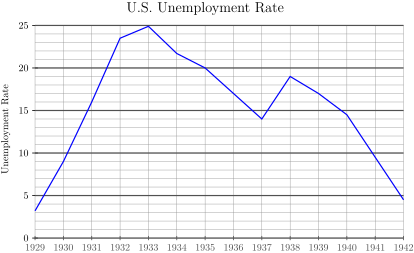
\includegraphics[width=\linewidth]{images/act1-1-1.png}
\end{sbspanel}%
\end{sidebyside}%
\par
%
\begin{enumerate}[label=\alph*]
\item{}What was the unemployment rate in 1930?%
\item{}When did the unemployment rate first reach 15\%?%
\item{}When did the unemplyment rate reach its highest value? What was the unemployment rate at that time?%
\item{}After 1930, when was the first time the unemployment rate fell below 10\%?%
\item{}During which year did the unemployment rate show the greatest increase? During which year did it show the greatest decrease?%
\item{}Complete the table:%
\begin{sidebyside}{1}{0}{0}{0}%
\begin{sbspanel}{1}%
{\centering%
{\tabularfont%
\begin{tabular}{AcAcAcAcA}\hrulethick
Year&\tablecelllines{c}{m}
{Unemployment\\
Rate}
&\tablecelllines{c}{m}
{Labor Force\\
(Millions)}
&\tablecelllines{c}{m}
{Number\\
Unemployed}
\tabularnewline\hrulethin
\(1929\)&\(\hphantom{0000}\)&\(48.0\)&\(\hphantom{0000}\)\tabularnewline\hrulethin
\(1930\)&\(\hphantom{0000}\)&\(48.8\)&\(\hphantom{0000}\)\tabularnewline\hrulethin
\(1931\)&\(\hphantom{0000}\)&\(49.6\)&\(\hphantom{0000}\)\tabularnewline\hrulethin
\(1932\)&\(\hphantom{0000}\)&\(50.3\)&\(\hphantom{0000}\)\tabularnewline\hrulethin
\(1933\)&\(\hphantom{0000}\)&\(51.1\)&\(\hphantom{0000}\)\tabularnewline\hrulethin
\(1934\)&\(\hphantom{0000}\)&\(51.9\)&\(\hphantom{0000}\)\tabularnewline\hrulethin
\(1935\)&\(\hphantom{0000}\)&\(52.6\)&\(\hphantom{0000}\)\tabularnewline\hrulethin
\(1936\)&\(\hphantom{0000}\)&\(53.3\)&\(\hphantom{0000}\)\tabularnewline\hrulethin
\(1937\)&\(\hphantom{0000}\)&\(54.1\)&\(\hphantom{0000}\)\tabularnewline\hrulethin
\(1938\)&\(\hphantom{0000}\)&\(54.9\)&\(\hphantom{0000}\)\tabularnewline\hrulethin
\(1939\)&\(\hphantom{0000}\)&\(55.6\)&\(\hphantom{0000}\)\tabularnewline\hrulethin
\(1940\)&\(\hphantom{0000}\)&\(56.2\)&\(\hphantom{0000}\)\tabularnewline\hrulethin
\(1941\)&\(\hphantom{0000}\)&\(57.5\)&\(\hphantom{0000}\)\tabularnewline\hrulethin
\(1942\)&\(\hphantom{0000}\)&\(60.4\)&\(\hphantom{0000}\)\tabularnewline\hrulethin
\end{tabular}
}%
\par}
\end{sbspanel}%
\end{sidebyside}%
\item{}During which year did the number of unemployed workers increase the most?%
\end{enumerate}
%
\end{activity}
\begin{activity}{Writing Mathematical Sentences.}{g:activity:idm46056784792400}%
\index{mathematical sentence}%
%
\begin{enumerate}[label=\arabic*]
\item{}Barry lives with his aunt while he attends college. Every week he gives her \textdollar{}20 from his paycheck to help pay for groceries. Fill in the table:%
\begin{sidebyside}{1}{0}{0}{0}%
\begin{sbspanel}{1}%
{\centering%
{\tabularfont%
\begin{tabular}{AcAcAcAcAcAcAcA}\hrulethick
Barry's paycheck&\(45\)&\(60\)&\(75\)&\(100\)&\(125\)&\(p\)\tabularnewline\hrulethin
Calculation&\(\blert{45-20}\)&\(\hphantom{0000}\)&\(\hphantom{0000}\)&\(\hphantom{0000}\)&\(\hphantom{0000}\)&\(\hphantom{0000}\)\tabularnewline\hrulethin
Amount he keeps&\(\blert{25}\)&\(\hphantom{0000}\)&\(\hphantom{0000}\)&\(\hphantom{0000}\)&\(\hphantom{0000}\)&\(\hphantom{0000}\)\tabularnewline\hrulethin
\end{tabular}
}%
\par}
\end{sbspanel}%
\end{sidebyside}%
\par
%
\begin{enumerate}[label=\alph*]
\item{}Explain in words how to find the amount Barry keeps from his paycheck.%
\item{}Write your explanation as a mathematical sentence:%
\par
Amount he keeps \(~=\)%
\item{}Let \(p\) stand for the amount of Barry's paycheck and \(k\) for the amount he keeps. Write an equation for \(k\) in terms of \(p\).%
\item{}Plot the points from the table and connect them with a smooth curve.%
\begin{sidebyside}{1}{0.25}{0.25}{0}%
\begin{sbspanel}{0.5}%
\includegraphics[width=\linewidth]{images/act1-1-2.png}
\end{sbspanel}%
\end{sidebyside}%
\end{enumerate}
%
\item{}Liz makes \textdollar{}6 an hour as a tutor in the Math Lab. Her wages for the week depend on the number of hours she works.  Fill in the table:%
\begin{sidebyside}{1}{0}{0}{0}%
\begin{sbspanel}{1}%
{\centering%
{\tabularfont%
\begin{tabular}{AcAcAcAcAcAcAcA}\hrulethick
Hours worked&\(3\)&\(5\)&\(6\)&\(8\)&\(15\)&\(h\)\tabularnewline\hrulethin
Calculation&\(\blert{6 \times 3}\)&\(\hphantom{0000}\)&\(\hphantom{0000}\)&\(\hphantom{0000}\)&\(\hphantom{0000}\)&\(\hphantom{0000}\)\tabularnewline\hrulethin
Wages&\(\blert{18}\)&\(\hphantom{0000}\)&\(\hphantom{0000}\)&\(\hphantom{0000}\)&\(\hphantom{0000}\)&\(\hphantom{0000}\)\tabularnewline\hrulethin
\end{tabular}
}%
\par}
\end{sbspanel}%
\end{sidebyside}%
\par
%
\begin{enumerate}[label=\alph*]
\item{}Explain in words how to find the Liz's wages for the week.%
\item{}Write your explanation as a mathematical sentence:%
\par
Wages \(~=\)%
\item{}Let \(h\) stand for the number of hours Liz worked and \(w\) for her wages. Write an equation for \(w\) in terms of \(h\).%
\item{}Plot the points from the table and connect them with a smooth curve.%
\begin{sidebyside}{1}{0.25}{0.25}{0}%
\begin{sbspanel}{0.5}%
\includegraphics[width=\linewidth]{images/act1-1-3.png}
\end{sbspanel}%
\end{sidebyside}%
\end{enumerate}
%
\end{enumerate}
%
\end{activity}
\end{introduction}%
%
%
\typeout{************************************************}
\typeout{Subsubsection  Wrap-Up}
\typeout{************************************************}
%
\begin{subsubsectionptx}{Wrap-Up}{}{Wrap-Up}{}{}{g:subsubsection:idm46056798264496}
\begin{objectives}{Objectives}{g:objectives:idm46056797107872}
In this Lesson we practiced the following skills:%
%
\begin{itemize}[label=\textbullet]
\item{}Reading values from a graph%
\item{}Plotting points from a table of values%
\item{}Describing a relationship between two variables%
\item{}Writing an equation relating two variables%
\end{itemize}
\end{objectives}
Questions to answer before the Homework Preview.%
\begin{outcomes}{Questions}{g:outcomes:idm46056797725488}
%
\begin{enumerate}[label=\arabic*]
\item{}In Activity 1e, how do we calculate the increase in unemployment rate?%
\item{}In Activity 1f, were more people unemployed in 1931 or in 1940?%
\item{}In Activity 2, is the first row of the table plotted on the horizontal axis or the vertical axis?%
\end{enumerate}
\end{outcomes}
\end{subsubsectionptx}
\end{subsectionptx}
%
%
\typeout{************************************************}
\typeout{Subsection  Homework Preview}
\typeout{************************************************}
%
\begin{subsectionptx}{Homework Preview}{}{Homework Preview}{}{}{g:subsection:idm46056799771072}
Here are exercises to try before the end of the class meeting.%
%
%
\typeout{************************************************}
\typeout{Exercises  Exercises}
\typeout{************************************************}
%
\begin{exercises-subsubsection}{Exercises}{}{Exercises}{}{}{g:exercises:idm46056797019008}
\par\medskip\noindent%
%
Write an equation for \(y\) in terms of \(x\).%
\begin{exercisegroupcol}{2}
\begin{divisionexerciseegcol}{1}{}{}{g:exercise:idm46056801032864}%
\begin{sidebyside}{1}{0}{0}{0}%
\begin{sbspanel}{1}%
{\centering%
{\tabularfont%
\begin{tabular}{AcAcAcAcAcA}\hrulethick
\(x\)&\(1\)&\(2\)&\(5\)&\(8\)\tabularnewline\hrulethin
\(y\)&\(9\)&\(10\)&\(13\)&\(16\)\tabularnewline\hrulethin
\end{tabular}
}%
\par}
\end{sbspanel}%
\end{sidebyside}%
\end{divisionexerciseegcol}%
\begin{divisionexerciseegcol}{2}{}{}{g:exercise:idm46056797844800}%
\begin{sidebyside}{1}{0}{0}{0}%
\begin{sbspanel}{1}%
{\centering%
{\tabularfont%
\begin{tabular}{AcAcAcAcAcA}\hrulethick
\(x\)&\(6\)&\(12\)&\(24\)&\(30\)\tabularnewline\hrulethin
\(y\)&\(1\)&\(2\)&\(4\)&\(5\)\tabularnewline\hrulethin
\end{tabular}
}%
\par}
\end{sbspanel}%
\end{sidebyside}%
\end{divisionexerciseegcol}%
\begin{divisionexerciseegcol}{3}{}{}{g:exercise:idm46056797430144}%
\begin{sidebyside}{1}{0}{0}{0}%
\begin{sbspanel}{1}%
{\centering%
{\tabularfont%
\begin{tabular}{AcAcAcAcAcA}\hrulethick
\(x\)&\(5\)&\(7\)&\(8\)&\(10\)\tabularnewline\hrulethin
\(y\)&\(3\)&\(5\)&\(6\)&\(8\)\tabularnewline\hrulethin
\end{tabular}
}%
\par}
\end{sbspanel}%
\end{sidebyside}%
\end{divisionexerciseegcol}%
\begin{divisionexerciseegcol}{4}{}{}{g:exercise:idm46056798265040}%
\begin{sidebyside}{1}{0}{0}{0}%
\begin{sbspanel}{1}%
{\centering%
{\tabularfont%
\begin{tabular}{AcAcAcAcAcA}\hrulethick
\(x\)&\(1\)&\(3\)&\(5\)&\(7\)\tabularnewline\hrulethin
\(y\)&\(4\)&\(12\)&\(20\)&\(28\)\tabularnewline\hrulethin
\end{tabular}
}%
\par}
\end{sbspanel}%
\end{sidebyside}%
\end{divisionexerciseegcol}%
\begin{divisionexerciseegcol}{5}{}{}{g:exercise:idm46056785596672}%
\begin{sidebyside}{1}{0}{0}{0}%
\begin{sbspanel}{1}%
{\centering%
{\tabularfont%
\begin{tabular}{AcAcAcAcAcA}\hrulethick
\(x\)&\(2\)&\(4\)&\(6\)&\(9\)\tabularnewline\hrulethin
\(y\)&\(10\)&\(8\)&\(6\)&\(3\)\tabularnewline\hrulethin
\end{tabular}
}%
\par}
\end{sbspanel}%
\end{sidebyside}%
\end{divisionexerciseegcol}%
\begin{divisionexerciseegcol}{6}{}{}{g:exercise:idm46056784805744}%
\begin{sidebyside}{1}{0}{0}{0}%
\begin{sbspanel}{1}%
{\centering%
{\tabularfont%
\begin{tabular}{AcAcAcAcAcA}\hrulethick
\(x\)&\(4\)&\(8\)&\(12\)&\(20\)\tabularnewline\hrulethin
\(y\)&\(3\)&\(6\)&\(8\)&\(15\)\tabularnewline\hrulethin
\end{tabular}
}%
\par}
\end{sbspanel}%
\end{sidebyside}%
\end{divisionexerciseegcol}%
\end{exercisegroupcol}
\par\medskip\noindent
\par\medskip\noindent%
%
Matt wants to travel 240 miles to visit a friend over spring break. He is deciding whether to ride his bike or drive. If he travels at an average speed of \(r\) miles per hour, then the trip will take \(t\) hours. Use the graph to answer the questions.%
\begin{sidebyside}{1}{0.15}{0.15}{0}%
\begin{sbspanel}{0.7}%
\includegraphics[width=\linewidth]{images/act1-1-4.png}
\end{sbspanel}%
\end{sidebyside}%
\begin{exercisegroup}
\begin{divisionexerciseeg}{7}{}{}{g:exercise:idm46056783038016}%
If Matt can ride at an average speed of 15 miles per hour, how long will the trip take?%
\end{divisionexerciseeg}%
\begin{divisionexerciseeg}{8}{}{}{g:exercise:idm46056783012080}%
If Matt wants to arrive in 8 hours, what average speed will he need to maintain?%
\end{divisionexerciseeg}%
\begin{divisionexerciseeg}{9}{}{}{g:exercise:idm46056783008624}%
How long will the trip take if Matt drives at 60 miles per hour?%
\end{divisionexerciseeg}%
\begin{divisionexerciseeg}{10}{}{}{g:exercise:idm46056782999872}%
If Matt doubles his speed, what happens to his travel time?%
\end{divisionexerciseeg}%
\end{exercisegroup}
\par\medskip\noindent
\end{exercises-subsubsection}
%
%
\typeout{************************************************}
\typeout{Solutions  Answers to Homework Preview}
\typeout{************************************************}
%
\begin{solutions-subsubsection}{Answers to Homework Preview}{}{Answers to Homework Preview}{}{}{g:solutions:idm46056782990624}
\begin{conclusion}{}%
%
\begin{multicols}{3}
\begin{enumerate}[label=\arabic*]
\item{}\(\displaystyle y=x+8\)%
\item{}\(\displaystyle y=x \div 6\)%
\item{}\(\displaystyle y=x-2\)%
\item{}\(\displaystyle y=4 \times x\)%
\item{}\(\displaystyle y=12-x\)%
\item{}\(\displaystyle y=\dfrac{3}{4} \times x\)%
\item{}16 hrs%
\item{}30 mph%
\item{}4 hrs%
\item{}Travel time is cut in half%
\end{enumerate}
\end{multicols}
%
\end{conclusion}%
\end{solutions-subsubsection}
\end{subsectionptx}
%
%
\typeout{************************************************}
\typeout{Exercises  Homework 1.1}
\typeout{************************************************}
%
\begin{exercises-subsection}{Homework 1.1}{}{Homework 1.1}{}{}{g:exercises:idm46056799390016}
\par\medskip\noindent%
%
For Problems 1\textendash{}4,%
\begin{enumerate}[label=\alph*]
\item{}Find the pattern and fill in the table.%
\item{}Write an equation for the second variable in terms of the first variable.%
\end{enumerate}
%
\begin{exercisegroupcol}{3}
\begin{divisionexerciseegcol}{1}{}{}{g:exercise:idm46056799477264}%
\begin{sidebyside}{1}{0}{0}{0}%
\begin{sbspanel}{1}%
{\centering%
{\tabularfont%
\begin{tabular}{AcAcA}\hrulethick
\(m\)&\(g\)\tabularnewline\hrulethin
\(2\)&\(5\)\tabularnewline\hrulethin
\(3\)&\(6\)\tabularnewline\hrulethin
\(5\)&\(8\)\tabularnewline\hrulethin
\(10\)&\(13\)\tabularnewline\hrulethin
\(12\)&\tabularnewline\hrulethin
\(16\)&\tabularnewline\hrulethin
\(18\)&\tabularnewline\hrulethin
\(m\)&\tabularnewline\hrulethin
\end{tabular}
}%
\par}
\end{sbspanel}%
\end{sidebyside}%
\end{divisionexerciseegcol}%
\begin{divisionexerciseegcol}{2}{}{}{g:exercise:idm46056764570336}%
\begin{sidebyside}{1}{0}{0}{0}%
\begin{sbspanel}{1}%
{\centering%
{\tabularfont%
\begin{tabular}{AcAcA}\hrulethick
\(t\)&\(w\)\tabularnewline\hrulethin
\(0\)&\(20\)\tabularnewline\hrulethin
\(2\)&\(18\)\tabularnewline\hrulethin
\(4\)&\(16\)\tabularnewline\hrulethin
\(5\)&\(15\)\tabularnewline\hrulethin
\(6\)&\tabularnewline\hrulethin
\(10\)&\tabularnewline\hrulethin
\(12\)&\tabularnewline\hrulethin
\(t\)&\tabularnewline\hrulethin
\end{tabular}
}%
\par}
\end{sbspanel}%
\end{sidebyside}%
\end{divisionexerciseegcol}%
\begin{divisionexerciseegcol}{3}{}{}{g:exercise:idm46056764632864}%
\begin{sidebyside}{1}{0}{0}{0}%
\begin{sbspanel}{1}%
{\centering%
{\tabularfont%
\begin{tabular}{AcAcA}\hrulethick
\(b\)&\(x\)\tabularnewline\hrulethin
\(0\)&\(0\)\tabularnewline\hrulethin
\(2\)&\(1\)\tabularnewline\hrulethin
\(4\)&\(2\)\tabularnewline\hrulethin
\(5\)&\(2.5\)\tabularnewline\hrulethin
\(6\)&\tabularnewline\hrulethin
\(8\)&\tabularnewline\hrulethin
\(9\)&\tabularnewline\hrulethin
\(b\)&\tabularnewline\hrulethin
\end{tabular}
}%
\par}
\end{sbspanel}%
\end{sidebyside}%
\end{divisionexerciseegcol}%
\end{exercisegroupcol}
\par\medskip\noindent
\begin{divisionexercise}{4}{}{}{g:exercise:idm46056764832640}%
\begin{sidebyside}{2}{0}{0}{0}%
\begin{sbspanel}{0.5}%
{\centering%
{\tabularfont%
\begin{tabular}{AcAcAcAcAcAcAcAcAcA}\hrulethick
\(z\)&\(3\)&\(6\)&\(8\)&\(12\)&\(15\)&\(18\)&\(20\)&\(z\)\tabularnewline\hrulethin
\(r\)&\(2\)&\(4\)&\(\dfrac{16}{3}\)&\(8\)&&&&\tabularnewline\hrulethin
\end{tabular}
}%
\par}
\end{sbspanel}%
\begin{sbspanel}{0.5}%
Hint:  What fraction can you multiply by \(z\) to get \(r\)?%
\end{sbspanel}%
\end{sidebyside}%
\end{divisionexercise}%
\par\medskip\noindent%
%
For Problems 5\textendash{}6, make your own table. Choose values for the first variable, and use the rule to find the values of the second variable.%
\begin{exercisegroupcol}{2}
\begin{divisionexerciseegcol}{5}{}{}{g:exercise:idm46056764908992}%
\(W = 1.2 \times n\)%
\begin{sidebyside}{1}{0}{0}{0}%
\begin{sbspanel}{1}%
{\centering%
{\tabularfont%
\begin{tabular}{AcAcAcAcAcAcA}\hrulethick
\(n\)&\(\hphantom{0000}\)&\(\hphantom{0000}\)&\(\hphantom{0000}\)&\(\hphantom{0000}\)&\(\hphantom{0000}\)\tabularnewline\hrulethin
\(W\)&\(\hphantom{0000}\)&\(\hphantom{0000}\)&\(\hphantom{0000}\)&\(\hphantom{0000}\)&\(\hphantom{0000}\)\tabularnewline\hrulethin
\end{tabular}
}%
\par}
\end{sbspanel}%
\end{sidebyside}%
\end{divisionexerciseegcol}%
\begin{divisionexerciseegcol}{6}{}{}{g:exercise:idm46056765037376}%
\(M = \dfrac{3}{2} \times x\)%
\begin{sidebyside}{1}{0}{0}{0}%
\begin{sbspanel}{1}%
{\centering%
{\tabularfont%
\begin{tabular}{AcAcAcAcAcAcA}\hrulethick
\(x\)&\(\hphantom{0000}\)&\(\hphantom{0000}\)&\(\hphantom{0000}\)&\(\hphantom{0000}\)&\(\hphantom{0000}\)\tabularnewline\hrulethin
\(M\)&\(\hphantom{0000}\)&\(\hphantom{0000}\)&\(\hphantom{0000}\)&\(\hphantom{0000}\)&\(\hphantom{0000}\)\tabularnewline\hrulethin
\end{tabular}
}%
\par}
\end{sbspanel}%
\end{sidebyside}%
\end{divisionexerciseegcol}%
\end{exercisegroupcol}
\par\medskip\noindent
\par\medskip\noindent%
%
For Problems 7\textendash{}8, fill in the tables. What do you notice? Explain.%
\begin{exercisegroup}
\begin{divisionexerciseeg}{7}{}{}{g:exercise:idm46056765104448}%
%
\begin{multicols}{3}
\begin{enumerate}[label=\alph*]
\item{}\(\displaystyle y = \dfrac{x}{8}\)%
\begin{sidebyside}{1}{0}{0}{0}%
\begin{sbspanel}{1}%
{\centering%
{\tabularfont%
\begin{tabular}{AcAcA}\hrulethick
\(x\)&\(y\)\tabularnewline\hrulethin
\(4\)&\(\)\tabularnewline\hrulethin
\(8\)&\(\)\tabularnewline\hrulethin
\(10\)&\(\)\tabularnewline\hrulethin
\(16\)&\(\)\tabularnewline\hrulethin
\end{tabular}
}%
\par}
\end{sbspanel}%
\end{sidebyside}%
\item{}\(\displaystyle y = \dfrac{1}{8} x\)%
\begin{sidebyside}{1}{0}{0}{0}%
\begin{sbspanel}{1}%
{\centering%
{\tabularfont%
\begin{tabular}{AcAcA}\hrulethick
\(x\)&\(y\)\tabularnewline\hrulethin
\(4\)&\(\)\tabularnewline\hrulethin
\(8\)&\(\)\tabularnewline\hrulethin
\(10\)&\(\)\tabularnewline\hrulethin
\(16\)&\(\)\tabularnewline\hrulethin
\end{tabular}
}%
\par}
\end{sbspanel}%
\end{sidebyside}%
\item{}\(\displaystyle y = 0.125 \times x\)%
\begin{sidebyside}{1}{0}{0}{0}%
\begin{sbspanel}{1}%
{\centering%
{\tabularfont%
\begin{tabular}{AcAcA}\hrulethick
\(x\)&\(y\)\tabularnewline\hrulethin
\(4\)&\(\)\tabularnewline\hrulethin
\(8\)&\(\)\tabularnewline\hrulethin
\(10\)&\(\)\tabularnewline\hrulethin
\(16\)&\(\)\tabularnewline\hrulethin
\end{tabular}
}%
\par}
\end{sbspanel}%
\end{sidebyside}%
\end{enumerate}
\end{multicols}
%
\end{divisionexerciseeg}%
\begin{divisionexerciseeg}{8}{}{}{g:exercise:idm46056765318848}%
%
\begin{multicols}{3}
\begin{enumerate}[label=\alph*]
\item{}\(\displaystyle y = \dfrac{3 \times x}{5}\)%
\begin{sidebyside}{1}{0}{0}{0}%
\begin{sbspanel}{1}%
{\centering%
{\tabularfont%
\begin{tabular}{AcAcA}\hrulethick
\(x\)&\(y\)\tabularnewline\hrulethin
\(5\)&\(\)\tabularnewline\hrulethin
\(10\)&\(\)\tabularnewline\hrulethin
\(12\)&\(\)\tabularnewline\hrulethin
\(1\)&\(\)\tabularnewline\hrulethin
\end{tabular}
}%
\par}
\end{sbspanel}%
\end{sidebyside}%
\item{}\(\displaystyle y = \dfrac{3}{5} \times x\)%
\begin{sidebyside}{1}{0}{0}{0}%
\begin{sbspanel}{1}%
{\centering%
{\tabularfont%
\begin{tabular}{AcAcA}\hrulethick
\(x\)&\(y\)\tabularnewline\hrulethin
\(5\)&\(\)\tabularnewline\hrulethin
\(10\)&\(\)\tabularnewline\hrulethin
\(12\)&\(\)\tabularnewline\hrulethin
\(1\)&\(\)\tabularnewline\hrulethin
\end{tabular}
}%
\par}
\end{sbspanel}%
\end{sidebyside}%
\item{}\(\displaystyle y = 0.6 \times x\)%
\begin{sidebyside}{1}{0}{0}{0}%
\begin{sbspanel}{1}%
{\centering%
{\tabularfont%
\begin{tabular}{AcAcA}\hrulethick
\(x\)&\(y\)\tabularnewline\hrulethin
\(5\)&\(\)\tabularnewline\hrulethin
\(10\)&\(\)\tabularnewline\hrulethin
\(12\)&\(\)\tabularnewline\hrulethin
\(1\)&\(\)\tabularnewline\hrulethin
\end{tabular}
}%
\par}
\end{sbspanel}%
\end{sidebyside}%
\end{enumerate}
\end{multicols}
%
\end{divisionexerciseeg}%
\end{exercisegroup}
\par\medskip\noindent
\begin{divisionexercise}{9}{}{}{g:exercise:idm46056765497712}%
The temperature in Sunnyvale is usually \(15 \degree\) hotter than it is in Ridgecrest, which is at a higher elevation. Fill in the table.%
\begin{sidebyside}{1}{0}{0}{0}%
\begin{sbspanel}{1}%
{\centering%
{\tabularfont%
\begin{tabular}{AcAcAcAcAcAcAcA}\hrulethick
Temperature in Ridgecrest&\(70\)&\(75\)&\(82\)&\(86\)&\(90\)&\(R\)\tabularnewline\hrulethin
Calculation&&&&&&\tabularnewline\hrulethin
Temperature in Sunnyvale&&&&&&\tabularnewline\hrulethin
\end{tabular}
}%
\par}
\end{sbspanel}%
\end{sidebyside}%
\par
%
\begin{enumerate}[label=\alph*]
\item{}Explain in words how to find the temperature in Sunnyvale.%
\item{}Write your explanation as a mathematical sentence:%
\par
\(\text{Temp in Sunnyvale} =\)%
\item{}Let \(R\) stand for the temperature in Ridgecrest and \(S\) for the temperature in Sunnyvale. Write an equation for \(S\) in terms of \(R\).%
\item{}Plot the points from the table and connect them with a smooth curve.%
\begin{sidebyside}{1}{0.3}{0.3}{0}%
\begin{sbspanel}{0.4}%
\resizebox{\linewidth}{!}{%
\tikzset{%
}
\begin{tikzpicture} [xscale=.075, yscale=.075]
\draw[cyan] (50,60) grid[step=5] (100,120);
\draw[black,thick, ->, >=stealth'] (50,60)--(107,60) node[right]{$R$};
\draw[black,thick, ->, >=stealth'] (50,60)--(50,127) node[left]{$S$};
\foreach \x in  {50, 60, ..., 100} {
 \draw[black, thick] (\x,60.75) --++(0,-1.5)  node[below]   {\x};
}
\foreach \y in  {60, 70, ..., 120} {
 \draw[black, thick] (50.75,\y) --++(-1.5,0)  node[left]   {\y};
}
\end{tikzpicture}
}%
\end{sbspanel}%
\end{sidebyside}%
\end{enumerate}
%
\end{divisionexercise}%
\begin{divisionexercise}{10}{}{}{g:exercise:idm46056765700624}%
Jerome is driving from his home in White Falls to his parents' home in Castle Heights, 200 miles away. Fill in the table.%
\begin{sidebyside}{1}{0}{0}{0}%
\begin{sbspanel}{1}%
{\centering%
{\tabularfont%
\begin{tabular}{AcAcAcAcAcAcAcA}\hrulethick
Miles driven&\(40\)&\(60\)&\(90\)&\(120\)&\(170\)&\(d\)\tabularnewline\hrulethin
Calculation&&&&&&\tabularnewline\hrulethin
Miles remaining&&&&&&\tabularnewline\hrulethin
\end{tabular}
}%
\par}
\end{sbspanel}%
\end{sidebyside}%
\par
%
\begin{enumerate}[label=\alph*]
\item{}Explain in words how to find the number of miles Jerome has left to drive.%
\item{}Write your explanation as a mathematical sentence:%
\par
\(\text{Miles remaining} =\)%
\item{}Let \(d\) stand for the number of miles Jerome has driven and \(r\) for the number of miles that remain. Write an equation for \(r\) in terms of \(d\).%
\item{}Plot the points from the table and connect them with a smooth curve.%
\begin{sidebyside}{1}{0.3}{0.3}{0}%
\begin{sbspanel}{0.4}%
\resizebox{\linewidth}{!}{%
\tikzset{%
}
\begin{tikzpicture} [scale=.02]
\draw[cyan] (0,0) grid[step=20] (200,200);
\draw[black,thick, ->, >=stealth'] (0,0)--(212,0) node[right]{$d$};
\draw[black,thick, ->, >=stealth'] (0,0)--(0,222) node[left]{$r$};
\foreach \x in  {100,200} {
 \draw[black, thick] (\x,0.75) --++(0,-1.5)  node[below]   {\x};
 \draw[black, thick] (0.75,\x) --++(-1.5,0)  node[left]   {\x};
}
\end{tikzpicture}
}%
\end{sbspanel}%
\end{sidebyside}%
\end{enumerate}
%
\end{divisionexercise}%
\begin{divisionexercise}{11}{}{}{g:exercise:idm46056765816592}%
Milton goes to a restaurant with two friends, and they agree to split the bill equally. Fill in the table.%
\begin{sidebyside}{1}{0}{0}{0}%
\begin{sbspanel}{1}%
{\centering%
{\tabularfont%
\begin{tabular}{AcAcAcAcAcAcAcA}\hrulethick
Total bill&\(15\)&\(30\)&\(45\)&\(75\)&\(81\)&\(b\)\tabularnewline\hrulethin
Calculation&&&&&&\tabularnewline\hrulethin
Milton's share&&&&&&\tabularnewline\hrulethin
\end{tabular}
}%
\par}
\end{sbspanel}%
\end{sidebyside}%
\par
%
\begin{enumerate}[label=\alph*]
\item{}Explain in words how to find Milton's share of the bill.%
\item{}Write your explanation as a mathematical sentence:%
\par
\(\text{Milton's share} =\)%
\item{}Let \(b\) stand for the bill and \(s\) for Milton's share. Write an equation for \(s\) in terms of \(b\).%
\item{}Plot the points from the table and connect them with a smooth curve.%
\begin{sidebyside}{1}{0.3}{0.3}{0}%
\begin{sbspanel}{0.4}%
\resizebox{\linewidth}{!}{%
\tikzset{%
}
\begin{tikzpicture} [xscale=.04, yscale=0.1]
\draw[cyan] (0,0) grid[xstep=10, ystep=4] (100,40);
\draw[black,thick, ->, >=stealth'] (0,0)--(107,0) node[right]{$b$};
\draw[black,thick, ->, >=stealth'] (0,0)--(0,45) node[left]{$s$};
\foreach \x in  {50, 100} {
 \draw[black, thick] (\x,0.75) --++(0,-1.5)  node[below]   {\x};
}
\foreach \y in  {8,16, ..., 40} {
 \draw[black, thick] (0.75,\y) --++(-1.5,0)  node[left]   {\y};
}
\end{tikzpicture}
}%
\end{sbspanel}%
\end{sidebyside}%
\end{enumerate}
%
\end{divisionexercise}%
\begin{divisionexercise}{12}{}{}{g:exercise:idm46056766515120}%
Nutrition experts tell us that no more than 30\% of the calories we consume should come from fat. Fill in the table with the fat calories allowed daily for various calorie levels.%
\begin{sidebyside}{1}{0}{0}{0}%
\begin{sbspanel}{1}%
{\centering%
{\tabularfont%
\begin{tabular}{AcAcAcAcAcAcAcA}\hrulethick
Total calories&\(1000\)&\(1500\)&\(2000\)&\(2500\)&\(3000\)&\(C\)\tabularnewline\hrulethin
Calculation&&&&&&\tabularnewline\hrulethin
Fat calories&&&&&&\tabularnewline\hrulethin
\end{tabular}
}%
\par}
\end{sbspanel}%
\end{sidebyside}%
\par
%
\begin{enumerate}[label=\alph*]
\item{}Explain in words how to find the number of fat calories allowed.%
\item{}Write your explanation as a mathematical sentence:%
\par
\(\text{Fat calories} =\)%
\item{}Let \(C\) stand for the number of calories and \(F\) for the number of fat calories. Write an equation for \(F\) in terms of \(C\).%
\item{}Plot the points from the table and connect them with a smooth curve.%
\begin{sidebyside}{1}{0.3}{0.3}{0}%
\begin{sbspanel}{0.4}%
\resizebox{\linewidth}{!}{%
\tikzset{%
}
\begin{tikzpicture} [xscale = 1.5, yscale=0.5]
\draw[cyan] (0,0) grid[xstep=0.2, ystep=.5] (3,10);
\draw[black,thick, ->, >=stealth'] (0,0)--(3.30,0) node[right]{$C$};
\draw[black,thick, ->, >=stealth'] (0,0)--(0,11) node[left]{$F$};
\foreach \x [evaluate=\x as \xi using int( 1000* \x )]  in  {1,2,3} {
 \draw[black, thick] (\x,0.225) --++(0,-.45)  node[below]   {\xi};
}
\foreach \y [evaluate=\y as \yi using int( 100* \y )]  in  {2,4,..., 10} {
 \draw[black, thick] (0.075,\y) --++(-.15,0)  node[left]   {\yi};
}
\end{tikzpicture}
}%
\end{sbspanel}%
\end{sidebyside}%
\end{enumerate}
%
\end{divisionexercise}%
\par\medskip\noindent%
%
Use the graphs to answer the questions in Problems 13\textendash{}14. You may have to estimate some of your answers.%
\begin{exercisegroup}
\begin{divisionexerciseeg}{13}{}{}{g:exercise:idm46056766601296}%
Suppose you invest \textdollar{}2000 in a retirement account that pays 8\% interest compounded continuously. The amount of money in the account each year is shown by the graph below.%
\begin{sidebyside}{1}{0.25}{0.25}{0}%
\begin{sbspanel}{0.5}%
\resizebox{\linewidth}{!}{%
\tikzset{%
}
\begin{tikzpicture} [xscale = 0.4,]
\draw[cyan] (0,0) grid[xstep=1, ystep=.2] (15,7);
\draw[black,thick, ->, >=stealth'] (0,0)--(15.7,0);
\draw[black,thick, ->, >=stealth'] (0,0)--(0,7.3);
\foreach \x  in  {2,4,...,14} {
 \draw[cyan, very thick] (\x,0) --++(0,7);
 \draw[black, thick] (\x,0.05) --++(0,-.1)  node[below]   {\x};
}
\foreach \y [evaluate=\y as \yi using int( 1000* \y )]  in  {1,2,..., 7} {
 \draw[cyan, very thick] (0, \y) --++(15,0);
 \draw[black, thick] (0.1,\y) --++(-.2,0)  node[left]   {\yi};
}
\node[label=left:\rotatebox{90}{Amount in account (in dollars)}] at (-2.5,3.5) {};
\node[below] at (8,-.5) {Number of years with account};
\draw[samples=65,domain=0:15,smooth,variable=\x,red,very thick, ->, >=stealth'] plot ({\x},{2*e^(.08*\x)});
\end{tikzpicture}
}%
\end{sbspanel}%
\end{sidebyside}%
\par
%
\begin{enumerate}[label=\alph*]
\item{}What variable is displayed on the horizontal axis?  The vertical axis?%
\item{}How much money will be in the account 5 years from now?%
\item{}When will the amount of money in the account exceed \textdollar{}6000?%
\item{}How much will the account grow between the second and third years?%
\item{}How much will the account grow between the twelfth and thirteenth years?%
\end{enumerate}
%
\end{divisionexerciseeg}%
\begin{divisionexerciseeg}{14}{}{}{g:exercise:idm46056766696816}%
Wendy brings a Thermos of soup for her lunch on a hike in the mountains.  When she pours the soup into a bowl, it begins to cool off. The graph below shows the temperature of the soup after it is served.%
\begin{sidebyside}{1}{0.25}{0.25}{0}%
\begin{sbspanel}{0.5}%
\resizebox{\linewidth}{!}{%
\tikzset{%
}
\begin{tikzpicture} [scale = 0.35]
\draw[cyan] (0,0) grid  (20,20);
\draw[black,thick, ->, >=stealth'] (0,0)--(21,0);
\draw[black,thick, ->, >=stealth'] (0,0)--(0,21);
\foreach \x  in  {2,4,...,20} {
 \draw[cyan, very thick] (\x,0) --++(0,20);
 \draw[black, thick] (\x,0.2) --++(0,-.2)  node[below]   {\x};
}
\foreach \y [evaluate=\y as \yi using int( 10* \y )]  in  {2,4,...,20} {
 \draw[cyan, very thick] (0, \y) --++(20,0);
 \draw[black, thick] (0.1,\y) --++(-.2,0)  node[left]   {\yi};
}
\node[label=left:\rotatebox{90}{Temperature of soup (in $\degree$F)}] at (-2.5,10) {};
\node[below] at (10,-1.5) {Number of minutes after being poured};
\draw[samples=65,domain=0:20,smooth,variable=\x,red,very thick, ->, >=stealth'] plot ({\x},{6+12*2^(-\x/2)});
\end{tikzpicture}
}%
\end{sbspanel}%
\end{sidebyside}%
\par
%
\begin{enumerate}[label=\alph*]
\item{}What variable is displayed on the horizontal axis? The vertical axis?%
\item{}How long does it take the soup to cool below 100?%
\item{}What is the temperature of the soup after 8 minutes?%
\item{}How many degrees does the soup cool in the first 2 minutes?%
\item{}After a while, the temperature of the soup levels off at the same as the outside temperature. What was the outside temperature that day?%
\end{enumerate}
%
\end{divisionexerciseeg}%
\end{exercisegroup}
\par\medskip\noindent
\begin{divisionexercise}{15}{}{}{g:exercise:idm46056766744880}%
A cantaloupe is dropped from a tall building. Its speed increases until it hits the ground.  Which of the four graphs below best represents the speed of the cantaloupe? Explain why your choice is the best one.%
\begin{sidebyside}{1}{0.15}{0.15}{0}%
\begin{sbspanel}{0.7}%
\resizebox{\linewidth}{!}{%
\tikzset{%
}
\begin{tikzpicture} 
\coordinate (O) at (0,0);
\draw[black,thick, ->, >=stealth'] (O)--++(4.5,0) node[below,midway, align=center]{Time\\(a)};;
\draw[black,thick, ->, >=stealth'] (O)--++(0,3) node[midway,label=left:\rotatebox{90}{Speed}]  {};;
\draw[red, ultra thick] (O)--++(1.7,1.7)--++(2.6,0);


\coordinate (O) at (6,0);
\draw[black,thick, ->, >=stealth'] (O)--++(4.5,0) node[below,midway, align=center]{Time\\(b)};
\draw[black,thick, ->, >=stealth'] (O)--++(0,3) node[midway,label=left:\rotatebox{90}{Speed}]  {};;
\draw[red, ultra thick] (O)++(0,2.2)--++(1,0)--++(1,-2.2)--++(2.3,0);


\coordinate (O) at (0,-4.2);
\draw[black,thick, ->, >=stealth'] (O)--++(4.5,0) node[below,midway, align=center]{Time\\(c)};;
\draw[black,thick, ->, >=stealth'] (O)--++(0,3) node[midway,label=left:\rotatebox{90}{Speed}]  {};;
\draw[red, ultra thick] (O)--++(1.7,1.7)--++(0.1,-1.7)--++(2.4,0);


\coordinate (O) at (6,-4.2);
\draw[black,thick, ->, >=stealth'] (O)--++(4.5,0) node[below,midway, align=center]{Time\\(d)};
\draw[black,thick, ->, >=stealth'] (O)--++(0,3) node[midway,label=left:\rotatebox{90}{Speed}]  {};;
\draw[red, ultra thick] (O)--++(2.1,1.8)--++(2.1,-1.8);
\end{tikzpicture}
}%
\end{sbspanel}%
\end{sidebyside}%
\end{divisionexercise}%
\begin{divisionexercise}{16}{}{}{g:exercise:idm46056780676704}%
%
\begin{enumerate}[label=\alph*]
\item{}Match each of the following stories with the appropriate graph.%
\begin{enumerate}[label=\Roman*]
\item{}Delbert walks directly from home to school, then stays there.%
\item{}Delbert walks towards school, but stops at a coffee shop for a cappuccino, then he goes on to school and stays there.%
\item{}Delbert walks toward school, but decides to return home, where he stays.%
\end{enumerate}
%
\item{}Write your own story for the remaining graph.%
\end{enumerate}
%
\begin{sidebyside}{1}{0.2}{0.2}{0}%
\begin{sbspanel}{0.6}%
\resizebox{\linewidth}{!}{%
\tikzset{%
}
\begin{tikzpicture} 
\coordinate (O) at (0,0);
\draw[black,thick, ->, >=stealth'] (O)--++(4.5,0) node[below,midway, align=center]{Time\\(a)};;
\draw[black,thick, ->, >=stealth'] (O)--++(0,3) node[midway,label=left:\rotatebox{90}{Distance from home}]  {};;
\draw[red, ultra thick] (O)--++(.75,1.)--++(.75,-1.)--++(2.8,0);

\coordinate (O) at (6,0);
\draw[black,thick, ->, >=stealth'] (O)--++(4.5,0) node[below,midway, align=center]{Time\\(b)};
\draw[black,thick, ->, >=stealth'] (O)--++(0,3) node[midway,label=left:\rotatebox{90}{Distance from home}]  {};;
\draw[red, ultra thick] (O)--++(.75,1.)--++(.75,-1.)--++(0.6,0)--++(1.5,2)--++(0.7,0);

\coordinate (O) at (0,-4.2);
\draw[black,thick, ->, >=stealth'] (O)--++(4.5,0) node[below,midway, align=center]{Time\\(c)};;
\draw[black,thick, ->, >=stealth'] (O)--++(0,3) node[midway,label=left:\rotatebox{90}{Distance from home}]  {};;
\draw[red, ultra thick] (O)--++(1.2,1.8)--++(3.1,0);

\coordinate (O) at (6,-4.2);
\draw[black,thick, ->, >=stealth'] (O)--++(4.5,0) node[below,midway, align=center]{Time\\(d)};
\draw[black,thick, ->, >=stealth'] (O)--++(0,3) node[midway,label=left:\rotatebox{90}{Distance from home}]  {};;
\draw[red, ultra thick] (O)--++(0.6,0.9)--++(.5,0)--++(0.6,0.9)--++(2.6,0);
\end{tikzpicture}
}%
\end{sbspanel}%
\end{sidebyside}%
\end{divisionexercise}%
\begin{divisionexercise}{17}{}{}{g:exercise:idm46056768468928}%
Plot each pair of values on the grid provided. Connect the points with a smooth curve. Which graph appears to be a straight line?%
\begin{multicols}{2}
\begin{enumerate}[label=\alph*]
\item{}\begin{sidebyside}{1}{0}{0}{0}%
\begin{sbspanel}{1}%
{\centering%
{\tabularfont%
\begin{tabular}{AcAcAcAcAcAcAcA}\hrulethick
\(t\)&\(0\)&\(1\)&\(2\)&\(5\)&\(6\)&\(8\)\tabularnewline\hrulethin
\(v\)&\(16\)&\(14\)&\(12\)&\(6\)&\(4\)&\(0\)\tabularnewline\hrulethin
\end{tabular}
}%
\par}
\end{sbspanel}%
\end{sidebyside}%
 \begin{sidebyside}{1}{0}{0}{0}%
\begin{sbspanel}{1}%
\resizebox{\linewidth}{!}{%
\tikzset{%
}
\begin{tikzpicture} [xscale = 0.75, yscale=0.3]
\draw[cyan] (0,0) grid[ystep=2]  (8,20);
\draw[black,thick, ->, >=stealth'] (0,0)--(8.6,0) node[right]{$t$};
\draw[black,thick, ->, >=stealth'] (0,0)--(0,22) node[left]{$v$};
\foreach \x  in  {5} {
 \draw[cyan, very thick] (\x,0) --++(0,20);
 \draw[black, thick] (\x,0.2) --++(0,-.4)  node[below] {\x};
}
\foreach \y in  {10,20} {
 \draw[cyan, very thick] (0, \y) --++(8,0);
 \draw[black, thick] (0.05,\y) --++(-.1,0)  node[left] {\y};
}
\node[below left] at (0,0) {0};
\end{tikzpicture}
}%
\end{sbspanel}%
\end{sidebyside}%
%
\item{}\begin{sidebyside}{1}{0}{0}{0}%
\begin{sbspanel}{1}%
{\centering%
{\tabularfont%
\begin{tabular}{AcAcAcAcAcAcAcA}\hrulethick
\(w\)&\(0\)&\(1\)&\(2\)&\(4\)&\(6\)&\(10\)\tabularnewline\hrulethin
\(Q\)&\(12\)&\(8\)&\(6\)&\(4\)&\(3\)&\(2\)\tabularnewline\hrulethin
\end{tabular}
}%
\par}
\end{sbspanel}%
\end{sidebyside}%
 \begin{sidebyside}{1}{0}{0}{0}%
\begin{sbspanel}{1}%
\resizebox{\linewidth}{!}{%
\tikzset{%
}
\begin{tikzpicture} [xscale = 0.6, yscale=0.5]
\draw[cyan] (0,0) grid[ystep=2]  (10,12);
\draw[black,thick, ->, >=stealth'] (0,0)--(10.6,0) node[right]{$w$};
\draw[black,thick, ->, >=stealth'] (0,0)--(0,12.8) node[left]{$Q$};
\foreach \x  in  {5,10} {
 \draw[cyan, very thick] (\x,0) --++(0,12);
 \draw[black, thick] (\x,0.1) --++(0,-.2)  node[below] {\x};
}
\foreach \y in  {5,10} {
 \draw[cyan, very thick] (0, \y) --++(10,0);
 \draw[black, thick] (0.05,\y) --++(-.1,0)  node[left] {\y};
}
\node[below left] at (0,0) {0};
\end{tikzpicture}
}%
\end{sbspanel}%
\end{sidebyside}%
%
\end{enumerate}
\end{multicols}
%
\end{divisionexercise}%
\begin{divisionexercise}{18}{}{}{g:exercise:idm46056783868096}%
\begin{sidebyside}{2}{0}{0.1}{0.05}%
\begin{sbspanel}{0.5}%
%
\begin{enumerate}[label=\alph*]
\item{}Read the graph at right to fill in the table.%
\begin{sidebyside}{1}{0}{0}{0}%
\begin{sbspanel}{1}%
{\centering%
{\tabularfont%
\begin{tabular}{AcAcAcAcAcAcAcA}\hrulethick
\(x\)&\(0\)&\(10\)&\(30\)&\(40\)&\(60\)&\(70\)\tabularnewline\hrulethin
\(y\)&&&&&&\tabularnewline\hrulethin
\end{tabular}
}%
\par}
\end{sbspanel}%
\end{sidebyside}%
\item{}Find a formula expressing \(y\) in terms of \(x\).%
\end{enumerate}
%
\end{sbspanel}%
\begin{sbspanel}{0.35}%
\resizebox{\linewidth}{!}{%
\tikzset{%
}
\begin{tikzpicture} [scale=0.05]
\draw[cyan] (0,0) grid[step=10]  (80,80);
\draw[black,thick, ->, >=stealth'] (0,0)--(86,0) node[right]{$x$};
\draw[black,thick, ->, >=stealth'] (0,0)--(0,89) node[left]{$y$};
\foreach \x  in  {20,40,60,80} {
 \draw[cyan, very thick] (\x,0) --++(0,80);
 \draw[black, thick] (\x,1) --++(0,-2)  node[below] {\x};
 \draw[cyan, very thick] (0,\x) --++(80,0);
 \draw[black, thick] (1,\x) --++(-2,0)  node[left] {\x};
}
\draw[red,very thick] (0,70)--(70,0);
\node[below left] at (0,0) {0};
\end{tikzpicture}
}%
\end{sbspanel}%
\end{sidebyside}%
\end{divisionexercise}%
\par\medskip\noindent%
%
For Problems 19\textendash{}20,%
\begin{enumerate}[label=\alph*]
\item{}Write an equation for the second variable in terms of the first variable.%
\item{}Fill in the table. Plot the points and connect them with a smooth curve.%
\end{enumerate}
%
\begin{exercisegroupcol}{2}
\begin{divisionexerciseegcol}{19}{}{}{g:exercise:idm46056767100768}%
\begin{sidebyside}{1}{0}{0}{0}%
\begin{sbspanel}{1}%
{\centering%
{\tabularfont%
\begin{tabular}{AcAcAcAcAcAcAcA}\hrulethick
\(x\)&\(0\)&\(0.2\)&\(0.3\)&\(0.5\)&\(0.6\)&\(0.7\)\tabularnewline\hrulethin
\(y\)&\(2\)&\(1.8\)&\(1.7\)&&&\tabularnewline\hrulethin
\end{tabular}
}%
\par}
\end{sbspanel}%
\end{sidebyside}%
\begin{sidebyside}{1}{0.05}{0.05}{0}%
\begin{sbspanel}{0.9}%
\resizebox{\linewidth}{!}{%
\tikzset{%
}
\begin{tikzpicture} [scale=3.4]
\draw[cyan] (0,0) grid[step=1/5]  (2,2);
\draw[black,thick, ->, >=stealth'] (0,0)--(2.15,0) node[right]{$x$};
\draw[black,thick, ->, >=stealth'] (0,0)--(0,2.15) node[left]{$y$};
\foreach \x  in  {0.2, 0.4, 0.6, 0.8,1,1.2,1.4,1.6,1.8, 2} {
 \draw[black, thick] (\x,.02) --++(0,-.04)  node[below] {\x};
 \draw[black, thick] (.02,\x) --++(-.04,0)  node[left] {\x};
}
 \draw[cyan, very thick] (1,0) --++(0,2);
 \draw[cyan, very thick] (0,1) --++(2,0);
 \draw[cyan, very thick] (2,0) --++(0,2);
 \draw[cyan, very thick] (0,2) --++(2,0);
\node[below left] at (0,0) {0};
\end{tikzpicture}
}%
\end{sbspanel}%
\end{sidebyside}%
\end{divisionexerciseegcol}%
\begin{divisionexerciseegcol}{20}{}{}{g:exercise:idm46056784691168}%
\begin{sidebyside}{1}{0}{0}{0}%
\begin{sbspanel}{1}%
{\centering%
{\tabularfont%
\begin{tabular}{AcAcAcAcAcAcAcA}\hrulethick
\(x\)&\(1\)&\(2\)&\(3\)&\(4\)&\(6\)&\(8\)\tabularnewline\hrulethin
\(y\)&\(120\)&\(60\)&\(40\)&&&\tabularnewline\hrulethin
\end{tabular}
}%
\par}
\end{sbspanel}%
\end{sidebyside}%
\begin{sidebyside}{1}{0.05}{0.05}{0}%
\begin{sbspanel}{0.9}%
\resizebox{\linewidth}{!}{%
\tikzset{%
}
\begin{tikzpicture} [xscale=0.6, yscale=.065]
\draw[cyan] (0,0) grid[ystep=5]  (12,120);
\draw[black,thick, ->, >=stealth'] (0,0)--(13,0) node[right]{$x$};
\draw[black,thick, ->, >=stealth'] (0,0)--(0,130) node[left]{$y$};
\foreach \x  in  {5,10} {
 \draw[black, thick] (\x,2) --++(0,-4)  node[below] {\x};
 \draw[cyan, very thick] (\x,0) --++(0,120);
}
\foreach \y  in  {25,50,75,100} {
 \draw[black, thick] (.15,\y) --++(-.3,0)  node[left] {\y};
 \draw[cyan, very thick] (0,\y) --++(12,0);
}
\node[below left] at (0,0) {0};
\end{tikzpicture}
}%
\end{sbspanel}%
\end{sidebyside}%
\end{divisionexerciseegcol}%
\end{exercisegroupcol}
\par\medskip\noindent
\end{exercises-subsection}
\end{sectionptx}
%
%
\typeout{************************************************}
\typeout{Section 1.2 Algebraic Expressions}
\typeout{************************************************}
%
\begin{sectionptx}{Algebraic Expressions}{}{Algebraic Expressions}{}{}{x:section:Algebraic-Expressions}
%
%
\typeout{************************************************}
\typeout{Subsection  Writing an Algebraic Expression}
\typeout{************************************************}
%
\begin{subsectionptx}{Writing an Algebraic Expression}{}{Writing an Algebraic Expression}{}{}{g:subsection:idm46056767288256}
\index{algebraic expression!writing}%
\index{expression}%
\begin{introduction}{}%
\begin{definition}{Algebraic expression.}{g:definition:idm46056767298624}%
\index{algebraic expression}%
\index{expression}%
An \terminology{algebraic expression}, or simply an \terminology{expression}, is any meaningful combination of numbers, variables, and operation symbols.%
\end{definition}
For example,%
\begin{equation*}
4 \times g,~~~~~~3 \times c + p,~~~~~~\text{and}~~~~~~\dfrac{n-7}{w}
\end{equation*}
are algebraic expressions. An important part of algebra involves translating word phrases into algebraic expressions.%
\begin{example}{}{x:example:Example-1-2-1}%
Write an algebraic expression for each quantity.%
\begin{enumerate}[label=\alph*]
\item{}30\% of the money invested in stocks%
\item{}The cost of the dinner split three ways%
\end{enumerate}
%
\par\smallskip%
\noindent\textbf{\blocktitlefont Solution}.\hypertarget{g:solution:idm46056767349312}{}\quad{}%
\begin{enumerate}[label=\alph*]
\item{}The amount invested is unknown, so we choose a variable to represent it.%
\begin{equation*}
\blert{\text{Amount invested in stocks:}~~~s}
\end{equation*}
Next, we identify the operation described:  "30\% of"  means 0.30 times:%
\begin{equation*}
\text{The expression is} ~~~~\blert{0.30s}
\end{equation*}
%
\item{}The cost of the dinner is unknown, so we choose a variable to represent it.%
\begin{equation*}
\blert{\text{Cost of dinner:}~~~C}
\end{equation*}
Next, we identify the operation described:  "Split" means divided:%
\begin{equation*}
\text{The expression is} ~~~~\blert{\dfrac{C}{3}}
\end{equation*}
%
\end{enumerate}
%
\end{example}
In the previous Example, we used three steps to write an algebraic expression.%
\begin{assemblage}{To write an algebraic expression.}{g:assemblage:idm46056767377568}%
%
\begin{enumerate}[label=\arabic*]
\item{}Identify the unknown quantity and write a short phrase to describe it.%
\item{}Choose a variable to represent the unknown quantity.%
\item{}Use mathematical symbols to represent the relationship.%
\end{enumerate}
%
\end{assemblage}
\end{introduction}%
%
%
\typeout{************************************************}
\typeout{Subsubsection  Reading Questions}
\typeout{************************************************}
%
\begin{subsubsectionptx}{Reading Questions}{}{Reading Questions}{}{}{g:subsubsection:idm46056767403296}
\begin{inlineexercise}{}{g:exercise:idm46056767415264}%
A meaningful combination of numbers, variables and operation symbols is called an \fillin{2.727272727272727}.%
\par\smallskip%
\noindent\textbf{\blocktitlefont Answer}.\hypertarget{g:answer:idm46056767430144}{}\quad{}algebraic expression%
\end{inlineexercise}
\end{subsubsectionptx}
\end{subsectionptx}
%
%
\typeout{************************************************}
\typeout{Subsection  Sums}
\typeout{************************************************}
%
\begin{subsectionptx}{Sums}{}{Sums}{}{}{g:subsection:idm46056767433296}
\index{sum}%
\index{sum|seealso{addition}}%
When we add two numbers \(a\) and \(b\), the result is called the \terminology{sum}\index{sum} of \(a\) and \(b\). We call the numbers \(a\) and \(b\) the \terminology{terms}\index{term!of the sum} of the sum.%
\begin{sidebyside}{1}{0.29}{0.29}{0}%
\begin{sbspanel}{0.42}%
\resizebox{\linewidth}{!}{%
\tikzset{%
}
\begin{tikzpicture} 
\coordinate (O) at (0,0);
\coordinate (A) at (-0.8,0.7);
\coordinate (Aa) at (-0.4,.25);
\coordinate (Ab) at (0.2,.25);
\coordinate (B) at (-.5,-.2);
\node at (O) {$2+3$};
\draw[blue, <-, >=stealth'] (Ab)--(A) node[left, scale=.9]{terms};
\draw[blue, <-, >=stealth'] (Aa)--(A);
\draw [blue,decorate,decoration={brace,amplitude=3pt}] (.5,-0.2)--(B)  node [below,midway,yshift=-4pt] {sum};
\coordinate (P) at (3,0);
\coordinate (C) at (3.6,0.7);
\coordinate (Ca) at (2.8,.2);
\coordinate (Cb) at (3.4,.23);
\coordinate (D) at (2.5,-.2);
\node at (P) {$x+5$};
\draw[blue, <-, >=stealth'] (Cb)--(C) node[right, scale=.9]{terms};
\draw[blue, <-, >=stealth'] (Ca)--(C);
\draw [blue,decorate,decoration={brace,amplitude=3pt}] (3.5,-0.2)--(D)  node [below,midway,yshift=-4pt] {sum};
\end{tikzpicture}
}%
\end{sbspanel}%
\end{sidebyside}%
\begin{example}{}{g:example:idm46056783875472}%
Write sums to represent the following phrases.%
\begin{multicols}{2}
\begin{enumerate}[label=\alph*]
\item{}Six more than \(x\)%
\item{}Fifteen greater than \(r\)%
\end{enumerate}
\end{multicols}
%
\par\smallskip%
\noindent\textbf{\blocktitlefont Solution}.\hypertarget{g:solution:idm46056767518368}{}\quad{}%
\begin{multicols}{2}
\begin{enumerate}[label=\alph*]
\item{}\(6+x\) or \(x+6\)%
\item{}\(15+r\) or \(r+15\)%
\end{enumerate}
\end{multicols}
%
\end{example}
The terms can be added in either order.  We call this fact the \terminology{commutative law} for addition.%
\begin{assemblage}{Commutative Law for Addition.}{g:assemblage:idm46056767548400}%
If \(a\) and \(b\) are numbers, then%
\begin{equation*}
\blert{a+b = b+a}
\end{equation*}
%
\end{assemblage}
\end{subsectionptx}
%
%
\typeout{************************************************}
\typeout{Subsection  Products}
\typeout{************************************************}
%
\begin{subsectionptx}{Products}{}{Products}{}{}{g:subsection:idm46056767570528}
\index{product}%
\index{product|seealso{multiplication}}%
\begin{introduction}{}%
When we multiply two numbers \(a\) and \(b\), the result is called the \terminology{product} of \(a\) and \(b\).  The numbers \(a\) and \(b\) are the \terminology{factors}\index{factor} of the product.%
\begin{assemblage}{Look Closer.}{g:assemblage:idm46056767614432}%
In arithmetic we use the symbol \(\times\) to denote multiplication. However, in algebra, \(\times\) may be confused with the variable \(x\). So, instead, we use a dot or parentheses for multiplication, like this:%
\begin{sidebyside}{1}{0.2}{0.2}{0}%
\begin{sbspanel}{0.6}%
\resizebox{\linewidth}{!}{%
\tikzset{%
}
\begin{tikzpicture} 
\coordinate (O) at (0,0);
\coordinate (A) at (-0.8,0.7);
\coordinate (Aa) at (-0.3,.2);
\coordinate (Ab) at (0.15,.25);
\coordinate (B) at (-.4,-.2);
\node at (O) {$2\cdot3$};
\draw[blue, <-, >=stealth'] (Ab)--(A) node[left, scale=.9]{factors};
\draw[blue, <-, >=stealth'] (Aa)--(A);
\draw [blue,decorate,decoration={brace,amplitude=3pt}] (.4,-0.2)--(B)  node [below,midway,yshift=-4pt] {product};
\coordinate (P) at (3.4,0);
\coordinate (C) at (2.8,0.7);
\coordinate (Ca) at (3.15,.25);
\coordinate (Cb) at (3.45,.25);
\coordinate (D) at (3,-.2);
\node at (P) {$2(3)$};
\draw[blue, <-, >=stealth'] (Cb)--(C) node[left, scale=.9]{factors};
\draw[blue, <-, >=stealth'] (Ca)--(C);
\draw [blue,decorate,decoration={brace,amplitude=3pt}] (3.8,-0.2)--(D)  node [below,midway,yshift=-4pt] {product};
\coordinate (Q) at (6.8,0);
\coordinate (E) at (6.2,0.7);
\coordinate (Ea) at (6.5,.25);
\coordinate (Eb) at (6.95,.25);
\coordinate (F) at (6.28,-.2);
\node at (Q) {$(2)(3)$};
\draw[blue, <-, >=stealth'] (Eb)--(E) node[left, scale=.9]{factors};
\draw[blue, <-, >=stealth'] (Ea)--(E);
\draw [blue,decorate,decoration={brace,amplitude=3pt}] (7.3,-0.2)--(F)  node [below,midway,yshift=-4pt] {product};
\end{tikzpicture}
}%
\end{sbspanel}%
\end{sidebyside}%
\par
If one of the factors is a variable, we can just write the factors side by side. For example,%
\begin{align*}
ab~~~~\amp \text{means} \amp\amp \text{the product of}~~ a~~ \text{times}~~ b\\
3x~~~~\amp \text{means} \amp\amp \text{the product of}~~ 3~~ \text{times}~~ x
\end{align*}
%
\end{assemblage}
\begin{example}{}{x:example:Example-1-2-3}%
Write products to represent the following phrases.%
\begin{enumerate}[label=\alph*]
\item{}Ten times \(z\)%
\item{}Two-thirds of \(y\)%
\item{}The product of \(x\) and \(y\)%
\end{enumerate}
%
\par\smallskip%
\noindent\textbf{\blocktitlefont Solution}.\hypertarget{g:solution:idm46056770739216}{}\quad{}%
\begin{multicols}{3}
\begin{enumerate}[label=\alph*]
\item{}\(\displaystyle 10z\)%
\item{}\(\displaystyle \dfrac{2}{3}y\)%
\item{}\(xy~~\) or \(~~yx\)%
\end{enumerate}
\end{multicols}
%
\end{example}
\begin{assemblage}{Look Closer.}{g:assemblage:idm46056770755648}%
In the previous Example, \(10z = 10 \cdot z = z \cdot 10\), because two numbers can be multiplied in either order to give the same answer. This is the \terminology{commutative law} for multiplication.%
\end{assemblage}
\begin{assemblage}{Commutative Law for Multiplication.}{g:assemblage:idm46056783724064}%
If \(a\) and \(b\) are numbers, then%
\begin{equation*}
\blert{a \cdot b = b \cdot a}
\end{equation*}
%
\end{assemblage}
In algebra, we usually write products with the numeral first. Thus, we write \(10z\) for "\(10\) times \(z\)”.%
\end{introduction}%
%
%
\typeout{************************************************}
\typeout{Subsubsection  Reading Questions}
\typeout{************************************************}
%
\begin{subsubsectionptx}{Reading Questions}{}{Reading Questions}{}{}{g:subsubsection:idm46056767655808}
\begin{inlineexercise}{}{g:exercise:idm46056767659824}%
When we add two numbers, the result is called the \fillin{2.727272727272727} and the two numbers are called the \fillin{2.727272727272727}.%
\par\smallskip%
\noindent\textbf{\blocktitlefont Answer}.\hypertarget{g:answer:idm46056767688656}{}\quad{}sum, terms%
\end{inlineexercise}
\begin{inlineexercise}{}{g:exercise:idm46056767689760}%
When we multiply two numbers, the result is called the \fillin{2.727272727272727} and the two numbers are called the \fillin{2.727272727272727}.%
\par\smallskip%
\noindent\textbf{\blocktitlefont Answer}.\hypertarget{g:answer:idm46056767704240}{}\quad{}product, factors%
\end{inlineexercise}
\end{subsubsectionptx}
\end{subsectionptx}
%
%
\typeout{************************************************}
\typeout{Subsection  Differences}
\typeout{************************************************}
%
\begin{subsectionptx}{Differences}{}{Differences}{}{}{g:subsection:idm46056767708864}
\index{difference}%
\index{difference|seealso{subtraction}}%
When we subtract \(b\) from \(a\) the result is called the \terminology{difference}\index{difference} of \(a\) and \(b\). As with addition, \(a\) and \(b\) are called \terminology{terms}\index{term!}.%
\begin{sidebyside}{1}{0.2}{0.2}{0}%
\begin{sbspanel}{0.6}%
\resizebox{\linewidth}{!}{%
\tikzset{%
}
\begin{tikzpicture} 
\coordinate (O) at (0,0);
\coordinate (A) at (-0.8,0.7);
\coordinate (Aa) at (-0.3,.2);
\coordinate (Ab) at (0.25,.2);
\coordinate (B) at (-.5,-.2);
\node at (O) {$a-b$};
\draw[blue, <-, >=stealth'] (Ab)--(A) node[left, scale=.9]{terms};
\draw[blue, <-, >=stealth'] (Aa)--(A);
\draw [blue,decorate,decoration={brace,amplitude=3pt}] (.5,-0.2)--(B)  node [below,midway,yshift=-4pt] {difference};
\coordinate (P) at (3.4,0);
\coordinate (C) at (2.8,0.7);
\coordinate (Ca) at (3.1,.25);
\coordinate (Cb) at (3.6,.2);
\coordinate (D) at (3,-.2);
\node at (P) {$8-c$};
\draw[blue, <-, >=stealth'] (Cb)--(C) node[left, scale=.9]{terms};
\draw[blue, <-, >=stealth'] (Ca)--(C);
\draw [blue,decorate,decoration={brace,amplitude=3pt}] (4.,-0.2)--(D)  node [below,midway,yshift=-4pt] {difference};
\coordinate (Q) at (6.8,0);
\coordinate (E) at (6.2,0.7);
\coordinate (Ea) at (6.5,.25);
\coordinate (Eb) at (7.05,.25);
\coordinate (F) at (6.28,-.2);
\node at (Q) {$5-2$};
\draw[blue, <-, >=stealth'] (Eb)--(E) node[left, scale=.9]{terms};
\draw[blue, <-, >=stealth'] (Ea)--(E);
\draw [blue,decorate,decoration={brace,amplitude=3pt}] (7.3,-0.2)--(F)  node [below,midway,yshift=-4pt] {difference};
\end{tikzpicture}
}%
\end{sbspanel}%
\end{sidebyside}%
\begin{warning}{}{g:warning:idm46056767777712}%
The difference \(5-2\) is not the same as \(2-5\).  When we translate "\(a\) subtracted from \(b\)," the order of the terms is important.%
\begin{equation*}
\begin{aligned}
b-a~~~~\amp \text{means} \amp\amp a~~ \text{subtracted from}~~ b\\ 
x-7~~~~\amp \text{means} \amp\amp 7~~ \text{subtracted from}~~  x\\
\end{aligned}
\end{equation*}
The operation of subtraction is not commutative.%
\end{warning}
\end{subsectionptx}
%
%
\typeout{************************************************}
\typeout{Subsection  Quotients}
\typeout{************************************************}
%
\begin{subsectionptx}{Quotients}{}{Quotients}{}{}{g:subsection:idm46056767800768}
\index{quotient}%
\index{quotient|seealso{division}}%
\begin{introduction}{}%
When we divide \(a\) by \(b\) the result is called the \terminology{quotient} of \(a\) and \(b\).  We call \(a\) the \terminology{dividend} and \(b\) the \terminology{divisor}.  In algebra we indicate division by using the division symbol, \(\div\), or a fraction bar.%
\begin{sidebyside}{1}{0.2}{0.2}{0}%
\begin{sbspanel}{0.6}%
\resizebox{\linewidth}{!}{%
\tikzset{%
}
\begin{tikzpicture} 
\coordinate (O) at (0,0);
\coordinate (A) at (0,0.8);
\coordinate (B) at (-.6,0.3);
\coordinate (B2) at (.65,0.3);
\coordinate (C) at (-.5,-0.2);
\node at (O) {$a\div b$};
\draw[blue, <-, >=stealth'] (A)++(0,-.5)--(A) node[above, yshift=-.3, scale=.9]{division symbol};
\draw[blue, <-, >=stealth'] (B)++(.2,-0.2)--(B) node[left, scale=.9] {dividend};;
\draw[blue, <-, >=stealth'] (B2)++(-.2,-0.2)--(B2) node[right, scale=.9] {divisor};;
\draw [blue,decorate,decoration={brace,amplitude=3pt}] (C)++(1,0)--(C)  node [below,midway,yshift=-4pt] {quotient};
\coordinate (P) at (5,0);
\coordinate (D) at (5,0.8);
\coordinate (E) at (4.4,0);
\coordinate (E2) at (5.25,0);
\coordinate (F) at (5,-.8);
\node at (P) {$\displaystyle\frac{a}{b}$};
\draw[blue, <-, >=stealth'] (D)++(0,-.35)--(D)--++(-0.3,0) node[left, scale=.9]{dividend};
\draw[blue, <-, >=stealth'] (E)++(.3,0)--(E) node[left, scale=.9] {fraction bar};;
\draw[blue, <-, >=stealth'] (F)++(0,.35)--(F)--++(0.3,0) node[right, scale=.9] {divisor};;
\draw [blue,decorate,decoration={brace,amplitude=3pt}] (E2)++(0,0.4)--++(0,-0.8)  node [right,midway,xshift=4pt] {quotient};
\end{tikzpicture}
}%
\end{sbspanel}%
\end{sidebyside}%
\begin{assemblage}{Look Closer.}{g:assemblage:idm46056767856176}%
The operation of division is not commutative. The order of the numbers in a quotient makes a difference. For example, \(12 \div 3 = 4\) but \(3 \div 12 = \dfrac{1}{4}\).%
\end{assemblage}
\begin{example}{}{g:example:idm46056767865520}%
Write an algebraic expression for each phrase.%
\begin{multicols}{2}
\begin{enumerate}[label=\alph*]
\item{}\(z\) subtracted from \(13\)%
\item{}\(25\) divided by \(R\)%
\end{enumerate}
\end{multicols}
%
\par\smallskip%
\noindent\textbf{\blocktitlefont Solution}.\hypertarget{g:solution:idm46056767889056}{}\quad{}%
\begin{multicols}{2}
\begin{enumerate}[label=\alph*]
\item{}\(\displaystyle 13-z\)%
\item{}\(\displaystyle \dfrac{25}{R}\)%
\end{enumerate}
\end{multicols}
%
\end{example}
\end{introduction}%
%
%
\typeout{************************************************}
\typeout{Subsubsection  Reading Questions}
\typeout{************************************************}
%
\begin{subsubsectionptx}{Reading Questions}{}{Reading Questions}{}{}{g:subsubsection:idm46056767897232}
\begin{inlineexercise}{}{g:exercise:idm46056767890608}%
Which operations obey the commutative laws? What do these laws say?%
\par\smallskip%
\noindent\textbf{\blocktitlefont Answer}.\hypertarget{g:answer:idm46056767907184}{}\quad{}addition and multiplication. We can add two numbers or multiply two numbers in either order.%
\end{inlineexercise}
\begin{inlineexercise}{}{g:exercise:idm46056767912768}%
When we subtract two numbers, the result is called the \fillin{2.727272727272727}.%
\par\smallskip%
\noindent\textbf{\blocktitlefont Answer}.\hypertarget{g:answer:idm46056767955648}{}\quad{}difference%
\end{inlineexercise}
\begin{inlineexercise}{}{g:exercise:idm46056767950928}%
When we divide two numbers, the result is called the \fillin{2.727272727272727}.%
\par\smallskip%
\noindent\textbf{\blocktitlefont Answer}.\hypertarget{g:answer:idm46056767968720}{}\quad{}quotient%
\end{inlineexercise}
\end{subsubsectionptx}
\end{subsectionptx}
%
%
\typeout{************************************************}
\typeout{Subsection  Evaluating an Algebraic Expression}
\typeout{************************************************}
%
\begin{subsectionptx}{Evaluating an Algebraic Expression}{}{Evaluating an Algebraic Expression}{}{}{g:subsection:idm46056767966912}
\index{evaluating!an algebraic expression}%
\index{algebraic expression!evaluating}%
An algebraic expression is a pattern or rule for different versions of the situation it describes. We can replace the variable by specific numbers to fit a particular situation.%
\begin{definition}{Evaluation.}{g:definition:idm46056767990512}%
\index{evaluating!an algebraic expression}%
\index{algebraic expression!evaluating}%
Substituting a specific value into an expression and calculating the result is called \terminology{evaluating} the expression.%
\end{definition}
\begin{example}{}{x:example:Example-1-2-5}%
Fernando has three roommates, and his share of the rent is \(\dfrac{R}{4}\), where \(R\) is a variable representing the total rent on the apartment. If Fernando and his roommates find an apartment whose rent is \textdollar{}540, we can find Fernando's share of the rent by replacing \(R\) by \(\alert{540}\).%
\begin{equation*}
\dfrac{R}{4} = \alert{540} \div 4 = 135
\end{equation*}
Fernando's share of the rent is \textdollar{}135.%
\end{example}
In the previous Example, we evaluated the expression \(\dfrac{R}{4}\) for \(R=540\).%
\end{subsectionptx}
%
%
\typeout{************************************************}
\typeout{Subsection  Some Useful Algebraic Formulas}
\typeout{************************************************}
%
\begin{subsectionptx}{Some Useful Algebraic Formulas}{}{Some Useful Algebraic Formulas}{}{}{x:subsection:useful-formulas}
\begin{introduction}{}%
Here are some examples of common formulas. Formulas may involve several different variables.%
\begin{assemblage}{Distance.}{g:assemblage:idm46056768042832}%
To find the distance traveled by an object moving at a constant speed or rate for a specified time, we multiply the rate by the time.%
\begin{equation*}
\blert{\text{distance} = \text{rate} \times \text{time}~~~~~~~~~~~~~d = rt}
\end{equation*}
%
\end{assemblage}
\begin{example}{}{g:example:idm46056768054608}%
How far will a train moving at 80 miles per hour travel in three hours?%
\par\smallskip%
\noindent\textbf{\blocktitlefont Solution}.\hypertarget{g:solution:idm46056768055856}{}\quad{}We evaluate the formula with \(r=\alert{80}\) and \(t=\alert{3}\) to find%
\begin{align*}
d \amp = rt\\
\amp = (\alert{80})(\alert{3}) = 240
\end{align*}
The train will travel 240 miles.%
\end{example}
\begin{assemblage}{Profit.}{g:assemblage:idm46056768066704}%
To find the \terminology{profit} earned by a company we subtract the costs from the revenue.%
\begin{equation*}
\blert{\text{profit} = \text{revenue} - \text{cost}~~~~~~~~~~~~~P = R-C}
\end{equation*}
%
\end{assemblage}
\begin{example}{}{g:example:idm46056768078224}%
The owner of a sandwich shop spent \textdollar{}800 last week for labor and supplies. She received \textdollar{}1150 in revenue.  What was her profit?%
\par\smallskip%
\noindent\textbf{\blocktitlefont Solution}.\hypertarget{g:solution:idm46056768084576}{}\quad{}We evaluate the formula with \(R=\alert{1150}\) and \(C=\alert{800}\) to find%
\begin{align*}
P \amp = R-C\\
\amp = \alert{1150}-\alert{350} = 350
\end{align*}
The owner's profit was \textdollar{}350.%
\end{example}
\begin{assemblage}{Interest.}{g:assemblage:idm46056768106368}%
To find the \terminology{interest} earned on an investment we multiply the amount invested (the principal) by the interest rate and the length of the investment.%
\begin{equation*}
\blert{\text{interest} = \text{principal} \times \text{interest rate} \times \text{time}~~~~~~~~~~~~~I=Prt}
\end{equation*}
%
\end{assemblage}
\begin{example}{}{g:example:idm46056768117776}%
How much interest will be earned on \textdollar{}800 invested for 3 years in a savings account that pays \(5\dfrac{1}{2}\)\% interest?%
\par\smallskip%
\noindent\textbf{\blocktitlefont Solution}.\hypertarget{g:solution:idm46056768131696}{}\quad{}We evaluate the formula with \(P=\alert{800}\), \(r=\alert{0.055}\), and \(t=\alert{3}\) to find%
\begin{align*}
I \amp = Prt\\
\amp = \alert{800} \times \alert{0.055} \times \alert{3} = 132
\end{align*}
The account will earn \textdollar{}132 in interest.%
\end{example}
\begin{assemblage}{Percent.}{g:assemblage:idm46056768145728}%
To find a percentage or \terminology{part} of a given amount, we multiply the whole amount by the percentage rate.%
\begin{equation*}
\blert{\text{part} = \text{percentage rate} \times \text{whole} ~~~~~~~~~~~~~P=rW}
\end{equation*}
%
\end{assemblage}
\begin{example}{}{g:example:idm46056768169856}%
How much ginger ale do you need to make 60 gallons of a fruit punch that is 20\% ginger ale?%
\par\smallskip%
\noindent\textbf{\blocktitlefont Solution}.\hypertarget{g:solution:idm46056768175584}{}\quad{}We evaluate the formula with \(r=\alert{0.20}\) and \(W=\alert{60}\) to find%
\begin{align*}
P \amp = rW\\
\amp = \alert{0.20} \times \alert{60} = 12
\end{align*}
You would need 12 gallons of ginger ale.%
\end{example}
\begin{assemblage}{Average.}{g:assemblage:idm46056768195568}%
To find the \terminology{average} of a collection of scores, we divide the sum of the scores by the number of scores.%
\begin{equation*}
\blert{\text{average score} = \dfrac{\text{sum of scores}}{\text{number of scores}} ~~~~~~~~~~~~~A=\dfrac{S}{n}}
\end{equation*}
%
\end{assemblage}
\begin{example}{}{g:example:idm46056768213824}%
Bert's quiz scores in chemistry are 15, 16, 18, 18, and 12.  What is his average score?%
\par\smallskip%
\noindent\textbf{\blocktitlefont Solution}.\hypertarget{g:solution:idm46056768219264}{}\quad{}We evaluate the formula with \(S=\alert{15+16+18+18+12}\) and \(n=\alert{5}\) to find%
\begin{align*}
A \amp = \dfrac{S}{n}\\
\amp = \dfrac{\alert{15+16+18+18+12}} {\alert{5}} = 15.8
\end{align*}
Bert's average score is 15.8.%
\end{example}
\end{introduction}%
%
%
\typeout{************************************************}
\typeout{Subsubsection  Reading Questions}
\typeout{************************************************}
%
\begin{subsubsectionptx}{Reading Questions}{}{Reading Questions}{}{}{g:subsubsection:idm46056768243248}
\begin{inlineexercise}{}{g:exercise:idm46056768244352}%
What does it mean to evaluate an expression?%
\par\smallskip%
\noindent\textbf{\blocktitlefont Answer}.\hypertarget{g:answer:idm46056768253440}{}\quad{}To substitute a specific value into the expression and calculate the result.%
\end{inlineexercise}
\begin{inlineexercise}{}{g:exercise:idm46056768183136}%
How do we change a percent to a decimal fraction?%
\par\smallskip%
\noindent\textbf{\blocktitlefont Answer}.\hypertarget{g:answer:idm46056768259344}{}\quad{}Move the decimal point 2 places to the left.%
\end{inlineexercise}
\begin{assemblage}{Look Ahead.}{g:assemblage:idm46056768260160}%
You will also need to know the formulas for the area and perimeter of a rectangle. See the Skills Warm-Up to review these formulas.%
\end{assemblage}
\end{subsubsectionptx}
\end{subsectionptx}
%
%
\typeout{************************************************}
\typeout{Subsection  Skills Warm-Up}
\typeout{************************************************}
%
\begin{subsectionptx}{Skills Warm-Up}{}{Skills Warm-Up}{}{}{g:subsection:idm46056768266576}
\begin{assemblage}{Good work!}{g:assemblage:idm46056768269120}%
You've finished the Reading assignment for Section 1.2.  Now try the Skills Warm-Up Exercises before the next class meeting.%
\end{assemblage}
%
%
\typeout{************************************************}
\typeout{Exercises  Exercises}
\typeout{************************************************}
%
\begin{exercises-subsubsection}{Exercises}{}{Exercises}{}{}{g:exercises:idm46056768272928}
\begin{introduction}{}%
Recall the formulas for the \terminology{area} and \terminology{perimeter} of a rectangle:%
\begin{equation*}
\blert{A = lw ~~~~~~~~\text{and} ~~~~~~~~P=2l+2w}
\end{equation*}
%
\end{introduction}%
\begin{divisionexercise}{1}{}{}{g:exercise:idm46056768286160}%
Delbert's living room is 20 feet long and 12 feet wide. How much oak baseboard does he need to border the floor? (Don't worry about doorways.)%
\end{divisionexercise}%
\begin{divisionexercise}{2}{}{}{g:exercise:idm46056768294448}%
How much wood parquet tiling must he buy to cover the floor?%
\end{divisionexercise}%
\par\medskip\noindent%
%
Which of the following phrases describe a perimeter, and which describe an area?%
\begin{exercisegroup}
\begin{divisionexerciseeg}{3}{}{}{g:exercise:idm46056768310496}%
The distance you jog around the shore of a small lake%
\end{divisionexerciseeg}%
\begin{divisionexerciseeg}{4}{}{}{g:exercise:idm46056768321488}%
The amount of Astroturf needed for the new football field%
\end{divisionexerciseeg}%
\begin{divisionexerciseeg}{5}{}{}{g:exercise:idm46056768323504}%
The amount of grated cheese needed to cover a pizza%
\end{divisionexerciseeg}%
\begin{divisionexerciseeg}{6}{}{}{g:exercise:idm46056768328256}%
The number of tulip bulbs needed to border a patio%
\end{divisionexerciseeg}%
\end{exercisegroup}
\par\medskip\noindent
\par\medskip\noindent%
%
Find the perimeter and area of each figure. All angles are right angles.%
\begin{exercisegroup}
\begin{divisionexerciseeg}{7}{}{}{g:exercise:idm46056768360000}%
\begin{sidebyside}{1}{0.325}{0.325}{0}%
\begin{sbspanel}{0.35}%
\resizebox{\linewidth}{!}{%
\tikzset{%
}
\begin{tikzpicture} [scale=0.8]
\draw[cyan, thick] (-3,0) grid (-2,5);
\draw[cyan, thick] (-2,0) grid (-1,4);
\draw[cyan, thick] (-1,0) grid (0,2);
\draw[cyan, thick] (0,0) grid (1,1);
\draw[cyan, thick] (3,0) grid (4,5);
\draw[cyan, thick] (2,0) grid (3,4);
\draw[cyan, thick] (1,0) grid (2,2);
\node[below,text=cyan] at (0.5,-0.4){All squares are};
\node[below,text=cyan] at (0.5,-1){1 centimeter on a side.};
\end{tikzpicture}
}%
\end{sbspanel}%
\end{sidebyside}%
\end{divisionexerciseeg}%
\begin{divisionexerciseeg}{8}{}{}{g:exercise:idm46056768379744}%
\begin{sidebyside}{1}{0.325}{0.325}{0}%
\begin{sbspanel}{0.35}%
\resizebox{\linewidth}{!}{%
\tikzset{%
}
\begin{tikzpicture} [scale=0.4]
\draw[red,very thick] (0,0)--++(0,5) node[left, midway, text=black]{5 ft};
\draw[red,very thick] (0,5)--++(8,0) node[above, midway, text=black]{8 ft};
\draw[red,very thick] (8,5)--++(0,3) node[left, midway, xshift=2, text=black]{3 ft};
\draw[red,very thick] (8,8)--++(4,0) node[above, midway, text=black]{4 ft};
\draw[red,very thick] (0,0)--++(3,0);
\draw[red,very thick] (3,0)--++(0,-2) node[left, midway, xshift=2, text=black]{2 ft};
\draw[red,very thick] (3,-2)--++(9,0) node[below, midway, text=black]{9 ft};
\draw[red, very thick](12,8)--++(0,-10);
\end{tikzpicture}
}%
\end{sbspanel}%
\end{sidebyside}%
\end{divisionexerciseeg}%
\end{exercisegroup}
\par\medskip\noindent
\end{exercises-subsubsection}
%
%
\typeout{************************************************}
\typeout{Solutions  Answers to Skills Warm-Up}
\typeout{************************************************}
%
\begin{solutions-subsubsection}{Answers to Skills Warm-Up}{}{Answers to Skills Warm-Up}{}{}{g:solutions:idm46056768397968}
\begin{conclusion}{}%
%
\begin{multicols}{3}
\begin{enumerate}[label=\arabic*]
\item{}64 ft%
\item{}240 sq ft%
\item{}perimeter%
\item{}area%
\item{}area%
\item{}perimeter%
\item{}32 cm; 23 sq cm%
\item{}44 ft; 90 sq ft%
\end{enumerate}
\end{multicols}
%
\end{conclusion}%
\end{solutions-subsubsection}
\end{subsectionptx}
%
%
\typeout{************************************************}
\typeout{Subsection  Lesson}
\typeout{************************************************}
%
\begin{subsectionptx}{Lesson}{}{Lesson}{}{}{g:subsection:idm46056768435200}
\begin{introduction}{}%
\begin{activity}{Writing Algebraic Expressions.}{g:activity:idm46056768443152}%
\index{algebraic expression!writing}%
\begin{assemblage}{To write an algebraic expression.}{g:assemblage:idm46056768447424}%
%
\begin{enumerate}[label=\arabic*]
\item{}Identify the unknown quantity and write a short phrase to describe it.%
\item{}Choose a variable to represent the unknown quantity.%
\item{}Use mathematical symbols to represent the relationship described.%
\end{enumerate}
%
\end{assemblage}
Study the Example below, then write expressions in the Exercise.%
\begin{example}{}{g:example:idm46056770865024}%
Write an algebraic expression for each quantity.%
\begin{enumerate}[label=\alph*]
\item{}3 feet more than the length of the rug%
\item{}Twice the age of the building%
\end{enumerate}
%
\par\smallskip%
\noindent\textbf{\blocktitlefont Solution}.\hypertarget{g:solution:idm46056770882224}{}\quad{}%
\begin{enumerate}[label=\alph*]
\item{}The length of the rug is unknown.%
\begin{equation*}
\blert{\text{Length of the rug:}~~~l}
\end{equation*}
The words "more than" indicate addition:%
\begin{equation*}
\blert{l+3}
\end{equation*}
%
\item{}The age of the building is unknown.%
\begin{equation*}
\blert{\text{Age of the building:}~~~a}
\end{equation*}
"Twice" means two times:%
\begin{equation*}
\blert{2a}
\end{equation*}
%
\end{enumerate}
%
\end{example}
EXERCISE 1. Write an algebraic expression for each quantity.%
\begin{enumerate}[label=\alph*]
\item{}Ten more than the number of students%
\item{}Five times the height of the triangle%
\item{}4\% of the original price%
\item{}Two and a quarter inches taller than last year's height%
\end{enumerate}
%
\par
The next example involves subtraction and division.%
\begin{example}{}{g:example:idm46056770920384}%
Write an algebraic expression for each quantity.%
\begin{enumerate}[label=\alph*]
\item{}5 square feet less than the area of the circle%
\item{}The ratio of your quiz score to 20%
\end{enumerate}
%
\par\smallskip%
\noindent\textbf{\blocktitlefont Solution}.\hypertarget{g:solution:idm46056770935920}{}\quad{}%
\begin{enumerate}[label=\alph*]
\item{}The area of the circle is unknown%
\begin{equation*}
\blert{\text{Area of circle:}~~~a}
\end{equation*}
The words "less than" indicate subtraction:%
\begin{equation*}
\blert{A-5}
\end{equation*}
%
\item{}Your quiz score is unknown.%
\begin{equation*}
\blert{\text{Quiz score:}~~~s}
\end{equation*}
"Twice" means two times:%
\begin{equation*}
\blert{\dfrac{s}{20}}
\end{equation*}
%
\end{enumerate}
%
\end{example}
EXERCISE 2. Write an algebraic expression for each quantity.%
\begin{enumerate}[label=\alph*]
\item{}\textdollar{}60 less than first-class airfare%
\item{}The quotient of the volume of the sphere and 6%
\item{}The ratio of the number of gallons of alcohol to 20%
\item{}The current population diminished by 50%
\end{enumerate}
%
\par
EXERCISE 3. Each of the words listed refers to one of the four arithmetic operations.  Group them under the correct operation.%
\begin{multicols}{3}
\begin{itemize}[label=\textbullet]
\item{}times%
\item{}take away%
\item{}sum of%
\item{}divided by%
\item{}less than%
\item{}reduced by%
\item{}twice%
\item{}fraction of%
\item{}increased by%
\item{}product of%
\item{}more than%
\item{}quotient of%
\item{}exceeded by%
\item{}deducted from%
\item{}ratio of%
\item{}total%
\item{}difference of%
\item{}split%
\item{}minus%
\item{}per%
\end{itemize}
\end{multicols}
%
\par
%
\begin{multicols}{2}
\begin{enumerate}[label=\alph*]
\item{}addition%
\item{}subtraction%
\item{}multiplication%
\item{}division%
\end{enumerate}
\end{multicols}
%
\end{activity}
\begin{activity}{Evaluating Algebraic Expressions.}{g:activity:idm46056771052304}%
\index{algebraic expression!evaluating}%
\index{evaluating an algebraic expression}%
\index{evaluating an algebraic expression|seealso{algebraic expression}}%
\begin{example}{}{g:example:idm46056771069328}%
The Appliance Mart is having a store wide 15\%-off sale. If the regular price of an appliance is \(P\) dollars, then the sale price \(S\) is given by the expression%
\begin{equation*}
S=0.85P
\end{equation*}
What is the sale price of a refrigerator that regularly sells for \textdollar{}600?%
\par\smallskip%
\noindent\textbf{\blocktitlefont Solution}.\hypertarget{g:solution:idm46056771085392}{}\quad{}We substitute \(\alert{600}\) for the regular price, \(P\), in the expression.%
\begin{align*}
S \amp = 0.85P\\
\amp = 0.85(\alert{600}) = 510
\end{align*}
The sale price is \textdollar{}510.%
\end{example}
EXERCISE 1: Evaluate the algebraic expression in the Example above to complete the table below showing the sale price for various appliances.%
\begin{sidebyside}{1}{0}{0}{0}%
\begin{sbspanel}{1}%
{\centering%
{\tabularfont%
\begin{tabular}{AcAcAcAcAcAcA}\hrulethick
\(P\)&\(120\)&\(200\)&\(380\)&\(480\)&\(520\)\tabularnewline\hrulethin
\(S\)&\(\hphantom{0000}\)&\(\hphantom{0000}\)&\(\hphantom{0000}\)&\(\hphantom{0000}\)&\(\hphantom{0000}\)\tabularnewline\hrulethin
\end{tabular}
}%
\par}
\end{sbspanel}%
\end{sidebyside}%
\par
Complete each table below by evaluating the expression.%
\begin{sidebyside}{2}{0}{0}{0.1}%
\begin{sbspanel}{0.45}%
2.%
\par
{\centering%
{\tabularfont%
\begin{tabular}{AcAcAcAcAcA}\hrulethick
\(x\)&\(1\)&\(2\)&\(10\)&\(100\)\tabularnewline\hrulethin
\(0.65x\)&\(\hphantom{0000}\)&\(\hphantom{0000}\)&\(\hphantom{0000}\)&\(\hphantom{0000}\)\tabularnewline\hrulethin
\end{tabular}
}%
\par}
\end{sbspanel}%
\begin{sbspanel}{0.45}%
3.%
\par
{\centering%
{\tabularfont%
\begin{tabular}{AcAcAcAcAcA}\hrulethick
\(n\)&\(0.1\)&\(0.5\)&\(0.75\)&\(1\)\tabularnewline\hrulethin
\(n-0.05\)&\(\hphantom{0000}\)&\(\hphantom{0000}\)&\(\hphantom{0000}\)&\(\hphantom{0000}\)\tabularnewline\hrulethin
\end{tabular}
}%
\par}
\end{sbspanel}%
\end{sidebyside}%
\begin{sidebyside}{2}{0}{0}{0.1}%
\begin{sbspanel}{0.45}%
4.%
\par
{\centering%
{\tabularfont%
\begin{tabular}{AcAcAcAcAcA}\hrulethick
\(a\)&\(6\)&\(8\)&\(\dfrac{3}{4}\)&\(\dfrac{6}{5}\)\tabularnewline\hrulethin
\(\dfrac{2}{3}a\)&\(\hphantom{0000}\)&\(\hphantom{0000}\)&\(\hphantom{0000}\)&\(\hphantom{0000}\)\tabularnewline\hrulethin
\end{tabular}
}%
\par}
\end{sbspanel}%
\begin{sbspanel}{0.45}%
5.%
\par
{\centering%
{\tabularfont%
\begin{tabular}{AcAcAcAcAcA}\hrulethick
\(h\)&\(1\)&\(\dfrac{5}{4}\)&\(2\dfrac{1}{2}\)&\(3\)\tabularnewline\hrulethin
\(h-\dfrac{3}{4}\)&\(\hphantom{0000}\)&\(\hphantom{0000}\)&\(\hphantom{0000}\)&\(\hphantom{0000}\)\tabularnewline\hrulethin
\end{tabular}
}%
\par}
\end{sbspanel}%
\end{sidebyside}%
\begin{sidebyside}{2}{0}{0}{0.1}%
\begin{sbspanel}{0.45}%
6.%
\par
{\centering%
{\tabularfont%
\begin{tabular}{AcAcAcAcAcA}\hrulethick
\(w\)&\(0.1\)&\(0.5\)&\(0.75\)&\(1.2\)\tabularnewline\hrulethin
\(2-w\)&\(\hphantom{0000}\)&\(\hphantom{0000}\)&\(\hphantom{0000}\)&\(\hphantom{0000}\)\tabularnewline\hrulethin
\end{tabular}
}%
\par}
\end{sbspanel}%
\begin{sbspanel}{0.45}%
7.%
\par
{\centering%
{\tabularfont%
\begin{tabular}{AcAcAcAcAcA}\hrulethick
\(p\)&\(0.1\)&\(0.5\)&\(1\)&\(4\)\tabularnewline\hrulethin
\(\dfrac{p}{0.4}\)&\(\hphantom{0000}\)&\(\hphantom{0000}\)&\(\hphantom{0000}\)&\(\hphantom{0000}\)\tabularnewline\hrulethin
\end{tabular}
}%
\par}
\end{sbspanel}%
\end{sidebyside}%
\end{activity}
\begin{activity}{Using Algebraic Formulas.}{g:activity:idm46056768528480}%
Write down the five algebraic formulas from the Reading, as algebraic expressions and in words.%
\begin{sidebyside}{1}{0}{0}{0}%
\begin{sbspanel}{1}%
{\centering%
{\tabularfont%
\begin{tabular}{AcAcAcA}\hrulethick
\(\hphantom{00}\)&Formula&Words\tabularnewline\hrulethin
1.&\(\hphantom{00000000000000}\)&\(\hphantom{0000000000000000000000000000000000000000}\)\tabularnewline\hrulethin
2.&\(\hphantom{00000000000000}\)&\(\hphantom{0000000000000000000000000000000000000000}\)\tabularnewline\hrulethin
3.&\(\hphantom{00000000000000}\)&\(\hphantom{0000000000000000000000000000000000000000}\)\tabularnewline\hrulethin
4.&\(\hphantom{00000000000000}\)&\(\hphantom{0000000000000000000000000000000000000000}\)\tabularnewline\hrulethin
5.&\(\hphantom{00000000000000}\)&\(\hphantom{0000000000000000000000000000000000000000}\)\tabularnewline\hrulethin
\end{tabular}
}%
\par}
\end{sbspanel}%
\end{sidebyside}%
\par
For the Exercises below, (a) Choose the appropriate formula and write an algebraic expression, and (b) Evaluate the expression to answer the question.%
\par
%
\begin{enumerate}[label=\arabic*]
\item{}It cost Ariel \textdollar{}380 to buy supplies and advertising for her pet-sitting business.%
\begin{enumerate}[label=\alph*]
\item{}Write an expression for her profit from the business.%
\item{}If Ariel earned \textdollar{}820 in revenue, what was her profit?%
\end{enumerate}
%
\item{}Jamie cycled for \(2\frac{1}{2}\) hours this morning.%
\begin{enumerate}[label=\alph*]
\item{}Write an expression for the distance Jamie cycled.%
\item{}If Jamie's average speed was 9 miles per hour, how far did she cycle?%
\end{enumerate}
%
\item{}SaveOurPark collected \textdollar{}2600 in donations from people in the neighborhood.%
\begin{enumerate}[label=\alph*]
\item{}Write an expression for the average amount that each person donated.%
\item{}If 142 people made a donation, what was the average donation?%
\end{enumerate}
%
\end{enumerate}
%
\end{activity}
\end{introduction}%
%
%
\typeout{************************************************}
\typeout{Subsubsection  Wrap-Up}
\typeout{************************************************}
%
\begin{subsubsectionptx}{Wrap-Up}{}{Wrap-Up}{}{}{g:subsubsection:idm46056768668400}
\begin{objectives}{Objectives}{g:objectives:idm46056768623984}
In this Lesson we practiced the following skills:%
%
\begin{itemize}[label=\textbullet]
\item{}Writing an algebraic expression%
\item{}Evaluating an algebraic expression%
\item{}Choosing an appropriate formula%
\end{itemize}
\end{objectives}
Questions to answer before the Homework Preview.%
\begin{outcomes}{Questions}{g:outcomes:idm46056768700768}
%
\begin{enumerate}[label=\arabic*]
\item{}What is the first step in evaluating an algebraic expression?%
\item{}What does it mean to evaluate an algebraic expression?%
\item{}Give definitions for the following terms:%
\par
\terminology{revenue},  \terminology{principal},  \terminology{percentage rate},  \terminology{average},  \terminology{perimeter}%
\end{enumerate}
\end{outcomes}
\end{subsubsectionptx}
\end{subsectionptx}
%
%
\typeout{************************************************}
\typeout{Subsection  Homework Preview}
\typeout{************************************************}
%
\begin{subsectionptx}{Homework Preview}{}{Homework Preview}{}{}{g:subsection:idm46056768743296}
Here are exercises to try before the end of the class meeting.%
%
%
\typeout{************************************************}
\typeout{Exercises  Exercises}
\typeout{************************************************}
%
\begin{exercises-subsubsection}{Exercises}{}{Exercises}{}{}{g:exercises:idm46056768749600}
\par\medskip\noindent%
%
Write algebraic expressions.%
\begin{exercisegroupcol}{2}
\begin{divisionexerciseegcol}{1}{}{}{g:exercise:idm46056768757712}%
The ratio of 6 to \(x\)%
\end{divisionexerciseegcol}%
\begin{divisionexerciseegcol}{2}{}{}{g:exercise:idm46056768761152}%
\(x\) decreased by 6%
\end{divisionexerciseegcol}%
\begin{divisionexerciseegcol}{3}{}{}{g:exercise:idm46056768767088}%
6\% of \(x\)%
\end{divisionexerciseegcol}%
\begin{divisionexerciseegcol}{4}{}{}{g:exercise:idm46056768773728}%
One-sixth of \(x\)%
\end{divisionexerciseegcol}%
\begin{divisionexerciseegcol}{5}{}{}{g:exercise:idm46056768775568}%
8 less than \(v\)%
\end{divisionexerciseegcol}%
\begin{divisionexerciseegcol}{6}{}{}{g:exercise:idm46056768780992}%
\(H\) increased by 14%
\end{divisionexerciseegcol}%
\end{exercisegroupcol}
\par\medskip\noindent
\par\medskip\noindent%
%
Choose a variable and write an algebraic expression.%
\begin{exercisegroup}
\begin{divisionexerciseeg}{7}{}{}{g:exercise:idm46056768788032}%
The ratio of your quiz score to 20%
\end{divisionexerciseeg}%
\begin{divisionexerciseeg}{8}{}{}{g:exercise:idm46056768793856}%
3 feet more than the length of the rug%
\end{divisionexerciseeg}%
\begin{divisionexerciseeg}{9}{}{}{g:exercise:idm46056768795472}%
Twice the age of the building%
\end{divisionexerciseeg}%
\begin{divisionexerciseeg}{10}{}{}{g:exercise:idm46056768798352}%
\textdollar{}6 less than the sales price%
\end{divisionexerciseeg}%
\end{exercisegroup}
\par\medskip\noindent
\par\medskip\noindent%
%
Use a formula to write an expression.%
\begin{exercisegroup}
\begin{divisionexerciseeg}{11}{}{}{g:exercise:idm46056768809648}%
Marla's revenue was \(D\) dollars, and her costs were \textdollar{}100. What was her profit?%
\end{divisionexerciseeg}%
\begin{divisionexerciseeg}{12}{}{}{g:exercise:idm46056768814880}%
Gertrude earned a total of \(P\) points on 5 quizzes.  What was her average score?%
\end{divisionexerciseeg}%
\begin{divisionexerciseeg}{13}{}{}{g:exercise:idm46056768824352}%
49.2\% of the voters favored your candidate.  If \(V\) people voted, how many favored your candidate?%
\end{divisionexerciseeg}%
\begin{divisionexerciseeg}{14}{}{}{g:exercise:idm46056768833936}%
The height of a triangle is 6 inches and its base is \(n\) inches. What is its area?%
\end{divisionexerciseeg}%
\end{exercisegroup}
\par\medskip\noindent
\end{exercises-subsubsection}
%
%
\typeout{************************************************}
\typeout{Solutions  Answers to Homework Preview}
\typeout{************************************************}
%
\begin{solutions-subsubsection}{Answers to Homework Preview}{}{Answers to Homework Preview}{}{}{g:solutions:idm46056768839696}
\begin{conclusion}{}%
%
\begin{multicols}{4}
\begin{enumerate}[label=\arabic*]
\item{}\(\displaystyle \dfrac{6}{x}\)%
\item{}\(\displaystyle x-6\)%
\item{}\(\displaystyle 0.06x\)%
\item{}\(\displaystyle \dfrac{1}{6}x\)%
\item{}\(\displaystyle v-8\)%
\item{}\(\displaystyle H+14\)%
\item{}\(\displaystyle \dfrac{Q}{20}\)%
\item{}\(\displaystyle L+3\)%
\item{}\(\displaystyle 2a\)%
\item{}\(\displaystyle S-6\)%
\item{}\(\displaystyle D-100\)%
\item{}\(\displaystyle \dfrac{P}{5}\)%
\item{}\(\displaystyle 0.492V\)%
\item{}\(\displaystyle 3n\)%
\end{enumerate}
\end{multicols}
%
\end{conclusion}%
\end{solutions-subsubsection}
\end{subsectionptx}
%
%
\typeout{************************************************}
\typeout{Exercises  Homework 1.2}
\typeout{************************************************}
%
\begin{exercises-subsection}{Homework 1.2}{}{Homework 1.2}{}{}{g:exercises:idm46056768911984}
\par\medskip\noindent%
%
For Problems 1\textendash{}10, write the word phrase as an algebraic expression.%
\begin{exercisegroupcol}{2}
\begin{divisionexerciseegcol}{1}{}{}{g:exercise:idm46056768938688}%
Product of 4 and \(y\)%
\end{divisionexerciseegcol}%
\begin{divisionexerciseegcol}{2}{}{}{g:exercise:idm46056768969040}%
Twice \(b\)%
\end{divisionexerciseegcol}%
\begin{divisionexerciseegcol}{3}{}{}{g:exercise:idm46056768975216}%
115\% of \(g\)%
\end{divisionexerciseegcol}%
\begin{divisionexerciseegcol}{4}{}{}{g:exercise:idm46056768995152}%
\(t\) decreased by 5%
\end{divisionexerciseegcol}%
\begin{divisionexerciseegcol}{5}{}{}{g:exercise:idm46056769008064}%
The quotient of 7 and \(w\)%
\end{divisionexerciseegcol}%
\begin{divisionexerciseegcol}{6}{}{}{g:exercise:idm46056769025024}%
4 divided into \(B\)%
\end{divisionexerciseegcol}%
\begin{divisionexerciseegcol}{7}{}{}{g:exercise:idm46056769033520}%
20 more than \(T\)%
\end{divisionexerciseegcol}%
\begin{divisionexerciseegcol}{8}{}{}{g:exercise:idm46056769048928}%
16 reduced by \(p\)%
\end{divisionexerciseegcol}%
\begin{divisionexerciseegcol}{9}{}{}{g:exercise:idm46056768916960}%
The ratio of 15 to \(M\)%
\end{divisionexerciseegcol}%
\begin{divisionexerciseegcol}{10}{}{}{g:exercise:idm46056769067712}%
The difference of \(R\) and 3.5%
\end{divisionexerciseegcol}%
\end{exercisegroupcol}
\par\medskip\noindent
\par\medskip\noindent%
%
For Problems 11\textendash{}14, choose the correct algebraic expression.%
\begin{assemblage}{}{g:assemblage:idm46056769076160}%
%
\begin{multicols}{3}
\begin{itemize}[label=\textbullet]
\item{}\(\displaystyle n+6\)%
\item{}\(\displaystyle n-6\)%
\item{}\(\displaystyle 6-n\)%
\item{}\(\displaystyle 6n\)%
\item{}\(\displaystyle \dfrac{n}{6}\)%
\item{}\(\displaystyle \dfrac{6}{n}\)%
\end{itemize}
\end{multicols}
%
\end{assemblage}
\begin{exercisegroup}
\begin{divisionexerciseeg}{11}{}{}{g:exercise:idm46056769099360}%
Rashad is 6 years younger than Shelley. If Shelley is \(n\) years old, how old is Rashad?%
\end{divisionexerciseeg}%
\begin{divisionexerciseeg}{12}{}{}{g:exercise:idm46056769110448}%
Each package of sodas contains 6 cans. If Antoine bought \(n\) packages of sodas, how many cans did he buy?%
\end{divisionexerciseeg}%
\begin{divisionexerciseeg}{13}{}{}{g:exercise:idm46056769146464}%
Lizette and Patrick together own 6 cats. If Lizette owns \(n\) cats, how many cats does Patrick own?%
\end{divisionexerciseeg}%
\begin{divisionexerciseeg}{14}{}{}{g:exercise:idm46056769179296}%
Mitra divided 6 cupcakes among \(n\) children.  How much of a cupcake did each child get?%
\end{divisionexerciseeg}%
\end{exercisegroup}
\par\medskip\noindent
\par\medskip\noindent%
%
For Problems 15\textendash{}17, write an algebraic expression for the area or perimeter of the figure. Include units in your answers. The dimensions are given in inches.%
\begin{exercisegroupcol}{3}
\begin{divisionexerciseegcol}{15}{}{}{g:exercise:idm46056769205280}%
\begin{sidebyside}{1}{0.1}{0.1}{0}%
\begin{sbspanel}{0.8}%
\includegraphics[width=\linewidth]{images/hp-1-2-15.png}
\end{sbspanel}%
\end{sidebyside}%
\par
area =%
\end{divisionexerciseegcol}%
\begin{divisionexerciseegcol}{16}{}{}{g:exercise:idm46056769219024}%
\begin{sidebyside}{1}{0.15}{0.15}{0}%
\begin{sbspanel}{0.7}%
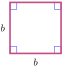
\includegraphics[width=\linewidth]{images/hp-1-2-16.png}
\end{sbspanel}%
\end{sidebyside}%
\par
perimeter =%
\end{divisionexerciseegcol}%
\begin{divisionexerciseegcol}{17}{}{}{g:exercise:idm46056769238272}%
\begin{sidebyside}{1}{0.05}{0.05}{0}%
\begin{sbspanel}{0.9}%
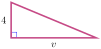
\includegraphics[width=\linewidth]{images/hp-1-2-17.png}
\end{sbspanel}%
\end{sidebyside}%
\par
area =%
\end{divisionexerciseegcol}%
\end{exercisegroupcol}
\par\medskip\noindent
\begin{divisionexercise}{18}{}{}{g:exercise:idm46056769259520}%
%
\begin{enumerate}[label=\alph*]
\item{}Which of these expressions says "one-sixth of \(x\)" ?%
\begin{equation*}
\dfrac{x}{6}~~~~~~\dfrac{6}{x}~~~~~~\dfrac{1}{6}x~~~~~\dfrac{1}{6x}
\end{equation*}
%
\item{}Which of these expressions says "6\% of \(x\)" ?%
\begin{equation*}
0.6x~~~~~~0.06x~~~~~~\dfrac{6}{100}x~~~~~~\dfrac{1}{6}x
\end{equation*}
%
\end{enumerate}
%
\end{divisionexercise}%
\begin{divisionexercise}{19}{}{}{g:exercise:idm46056769303776}%
Francine is saving up to buy a car, and deposits \(\dfrac{1}{5}\) of her spending money each month into a savings account.%
\begin{enumerate}[label=\alph*]
\item{}If \(m\) stands for Francine's spending money, write an expression for the amount she saves.%
\item{}Evaluate the expression to complete the table.%
\begin{sidebyside}{1}{0}{0}{0}%
\begin{sbspanel}{1}%
{\centering%
{\tabularfont%
\begin{tabular}{AcAcAcAcA}\hrulethick
Spending money (dollars)&\(20\)&\(25\)&\(60\)\tabularnewline\hrulethin
Amount saved (dollars)&&&\tabularnewline\hrulethin
\end{tabular}
}%
\par}
\end{sbspanel}%
\end{sidebyside}%
\end{enumerate}
%
\end{divisionexercise}%
\begin{divisionexercise}{20}{}{}{g:exercise:idm46056769450384}%
Delbert wants to enlarge his class photograph. Its height is \(\dfrac{1}{4}\) of its width. The enlarged photo should have the same shape as the original.%
\begin{enumerate}[label=\alph*]
\item{}If \(W\) stands for the width of the enlargement, write an expression for its height.%
\item{}Evaluate the expression to complete the table.%
\begin{sidebyside}{1}{0}{0}{0}%
\begin{sbspanel}{1}%
{\centering%
{\tabularfont%
\begin{tabular}{AcAcAcAcA}\hrulethick
Width of photo (inches)&\(6\)&\(10\)&\(24\)\tabularnewline\hrulethin
Height of photo (inches)&&&\tabularnewline\hrulethin
\end{tabular}
}%
\par}
\end{sbspanel}%
\end{sidebyside}%
\end{enumerate}
%
\end{divisionexercise}%
\begin{divisionexercise}{21}{}{}{g:exercise:idm46056769511728}%
If the governor vetoes a bill passed by the State Assembly, \(\dfrac{2}{3}\) of the members present must vote for the bill in order to overturn the veto.%
\begin{enumerate}[label=\alph*]
\item{}If \(p\) stands for the number of Assembly members present, write an expression for the number of votes needed to overturn a veto.%
\item{}Evaluate the expression to complete the table.%
\begin{sidebyside}{1}{0}{0}{0}%
\begin{sbspanel}{1}%
{\centering%
{\tabularfont%
\begin{tabular}{AcAcAcAcA}\hrulethick
Members present&\(90\)&\(96\)&\(120\)\tabularnewline\hrulethin
Votes needed&&&\tabularnewline\hrulethin
\end{tabular}
}%
\par}
\end{sbspanel}%
\end{sidebyside}%
\end{enumerate}
%
\end{divisionexercise}%
\begin{divisionexercise}{22}{}{}{g:exercise:idm46056769607312}%
Marla's investment club buys some stock. She will get \(\dfrac{3}{5}\) of the dividends.%
\begin{enumerate}[label=\alph*]
\item{}If \(D\) stands for the stock dividends, write an expression for Marla's share.%
\item{}Evaluate the expression to complete the table.%
\begin{sidebyside}{1}{0}{0}{0}%
\begin{sbspanel}{1}%
{\centering%
{\tabularfont%
\begin{tabular}{AcAcAcAcA}\hrulethick
Stock dividend&\(40\)&\(85\)&\(115\)\tabularnewline\hrulethin
Marla's share&\(24\)&\(51\)&\(69\)\tabularnewline\hrulethin
\end{tabular}
}%
\par}
\end{sbspanel}%
\end{sidebyside}%
\end{enumerate}
%
\end{divisionexercise}%
\par\medskip\noindent%
%
For Problems 23\textendash{}30, choose a variable for the unknown quantity and translate the phrase into an algebraic expression.%
\begin{exercisegroup}
\begin{divisionexerciseeg}{23}{}{}{g:exercise:idm46056769694672}%
The product of the ticket price and \textdollar{}15%
\end{divisionexerciseeg}%
\begin{divisionexerciseeg}{24}{}{}{g:exercise:idm46056769710224}%
Three times the cost of a light bulb%
\end{divisionexerciseeg}%
\begin{divisionexerciseeg}{25}{}{}{g:exercise:idm46056769719328}%
Three-fifths of the savings account balance%
\end{divisionexerciseeg}%
\begin{divisionexerciseeg}{26}{}{}{g:exercise:idm46056769737280}%
The price of the pizza divided by 6%
\end{divisionexerciseeg}%
\begin{divisionexerciseeg}{27}{}{}{g:exercise:idm46056769753968}%
The weight of the copper in ounces divided by 16%
\end{divisionexerciseeg}%
\begin{divisionexerciseeg}{28}{}{}{g:exercise:idm46056769757392}%
9\% of the school buses%
\end{divisionexerciseeg}%
\begin{divisionexerciseeg}{29}{}{}{g:exercise:idm46056769764432}%
\textdollar{}16 less than the cost of the vaccine%
\end{divisionexerciseeg}%
\begin{divisionexerciseeg}{30}{}{}{g:exercise:idm46056769777888}%
The total cost of 32 identical computers%
\end{divisionexerciseeg}%
\end{exercisegroup}
\par\medskip\noindent
\par\medskip\noindent%
%
For Problems 31\textendash{}32, write algebraic expressions in terms of \(x\).%
\begin{exercisegroup}
\begin{divisionexerciseeg}{31}{}{}{g:exercise:idm46056769797984}%
%
\begin{enumerate}[label=\alph*]
\item{}Daniel and Lara together made \textdollar{}480. If Daniel made \(x\) dollars, how much did Lara make?%
\item{}Alix spent \textdollar{}500 on tuition and books. If she spent \(x\) dollars on books, how much was her tuition?%
\item{}Thirty children signed up for summer camp. If \(x\) boys signed up, how many girls signed up?%
\end{enumerate}
%
\end{divisionexerciseeg}%
\begin{divisionexerciseeg}{32}{}{}{g:exercise:idm46056769857568}%
%
\begin{enumerate}[label=\alph*]
\item{}Rona spent \textdollar{}15 less than her sister on shoes. If Rona's sister spent \(x\) dollars, how much did Rona spend?%
\item{}Phoenix had 12 fewer rain days than Boston last year. If Boston had \(x\) rain days, how many rain days did Phoenix have?%
\item{}Jared scored 18 points lower on his second test than he scored on his first test. If he scored \(x\) points on the first test, what was his score on the second test?%
\end{enumerate}
%
\end{divisionexerciseeg}%
\end{exercisegroup}
\par\medskip\noindent
\par\medskip\noindent%
%
For Problems 33\textendash{}36, name the variable and write an algebraic expression.%
\begin{exercisegroup}
\begin{divisionexerciseeg}{33}{}{}{g:exercise:idm46056769908816}%
Eggnog is 70\% milk. Write an expression for the amount of milk in a container of eggnog.%
\end{divisionexerciseeg}%
\begin{divisionexerciseeg}{34}{}{}{g:exercise:idm46056769926560}%
Errol has saved \textdollar{}1200 for his vacation this year. Write an expression for the average amount he can spend on each day of his vacation.%
\end{divisionexerciseeg}%
\begin{divisionexerciseeg}{35}{}{}{g:exercise:idm46056769960384}%
Garth received 432 fewer votes than his opponent in the election. Write an expression for the number of votes Garth received.%
\end{divisionexerciseeg}%
\begin{divisionexerciseeg}{36}{}{}{g:exercise:idm46056769969232}%
The cost of the conference was \textdollar{}2000 over budget. Write an expression for the cost of the conference.%
\end{divisionexerciseeg}%
\end{exercisegroup}
\par\medskip\noindent
\par\medskip\noindent%
%
For Problems 37\textendash{}40, use the formulas in this Lesson.%
\begin{exercisegroup}
\begin{divisionexerciseeg}{37}{}{}{g:exercise:idm46056770009680}%
%
\begin{enumerate}[label=\alph*]
\item{}Write an equation for the distance \(d\) traveled in \(t\) hours by a small plane flying at 180 miles per hour.%
\item{}How far will the plane fly in 2 hours? In \(3\dfrac{1}{2}\) hours? In half a day?%
\end{enumerate}
%
\end{divisionexerciseeg}%
\begin{divisionexerciseeg}{38}{}{}{g:exercise:idm46056770045536}%
%
\begin{enumerate}[label=\alph*]
\item{}A certain pesticide contains 0.02\% by volume of a dangerous chemical. Write an equation for the amount of chemical \(C\) that enters the environment in terms of the number of gallons of pesticide used.%
\item{}How much of the chemical enters the environment if 400 gallons of the pesticide are used? 5000 gallons? 50,000 gallons?%
\end{enumerate}
%
\end{divisionexerciseeg}%
\begin{divisionexerciseeg}{39}{}{}{g:exercise:idm46056770068704}%
%
\begin{enumerate}[label=\alph*]
\item{}BioTech budgets 8.5\% of its revenue for research. Write an equation for the research budget \(B\) in terms of BioTech's revenue \(R\).%
\item{}What is the research budget if BioTech's revenue is \textdollar{}100,000? \textdollar{}500,000? \textdollar{}2,000,000?%
\end{enumerate}
%
\end{divisionexerciseeg}%
\begin{divisionexerciseeg}{40}{}{}{g:exercise:idm46056770095104}%
%
\begin{enumerate}[label=\alph*]
\item{}Hugo's Auto Shop paid \textdollar{}4000 in expenses this month. Write an equation for their profit \(P\) in terms of their revenue \(R\).%
\item{}What was their profit if their revenue was \textdollar{}10,000? \textdollar{}6500? \textdollar{}2500?%
\end{enumerate}
%
\end{divisionexerciseeg}%
\end{exercisegroup}
\par\medskip\noindent
\end{exercises-subsection}
\end{sectionptx}
%
%
\typeout{************************************************}
\typeout{Section 1.3 Equations and Graphs}
\typeout{************************************************}
%
\begin{sectionptx}{Equations and Graphs}{}{Equations and Graphs}{}{}{x:section:Equations-and-Graphs}
\index{graph}%
\index{graphing|see{graph}}%
%
%
\typeout{************************************************}
\typeout{Subsection  Anatomy of a Graph}
\typeout{************************************************}
%
\begin{subsectionptx}{Anatomy of a Graph}{}{Anatomy of a Graph}{}{}{g:subsection:idm46056770132768}
\index{graph}%
\begin{introduction}{}%
We use equations to express the relationship between two variabes. A graph is a way of visualizing an equation.%
\begin{assemblage}{Graph of an Equation.}{g:assemblage:idm46056770142112}%
A graph has two \terminology{axes}\index{axis}, horizontal and vertical, and the values for the variables are displayed along the axes. The first, or \terminology{input}\index{input!variable}, variable is displayed on the horizontal axis. \index{horizontal axis|see{\(x\)-axis}} The second, or \terminology{output}\index{output!variable}, variable is displayed on the vertical axis.\index{vertical axis|see{\(y\)-axis}}%
\end{assemblage}
The graph itself shows how the two variables are related.%
\begin{example}{}{x:example:Example-1-3-1}%
The graph below shows the relationship between Delbert's age, \(D\), and Francine's age, \(F\).  Write an equation for Francine's age in terms of Delbert's age.%
\begin{sidebyside}{1}{0.325}{0.325}{0}%
\begin{sbspanel}{0.35}%
\resizebox{\linewidth}{!}{%
\tikzset{%
}
\begin{tikzpicture} [scale=0.5]
\draw[cyan] (0,0) grid (10,15);
\draw[black,thick, ->, >=stealth'] (0,0)--(11,0) node[right]{$D$};
\draw[black,thick, ->, >=stealth'] (0,0)--(0,16) node[left]{$F$};
\foreach \x in  {5,10} {
 \draw[cyan, very thick] (\x,0) --++(0,15);
 \draw[black, thick] (\x,.1) --++(0,-.2)  node[below]   {\x};
}
\foreach \y in  {5,10,15} {
 \draw[cyan, very thick] (0,\y) --++(10,0);
 \draw[black, thick] (.1,\y) --++(-.2,0)  node[left]   {\y};
}
\filldraw[red] (3,7) circle (0.15cm) node[above left, xshift=-1, yshift=1, fill=white, inner sep = 1, text=black] {$P$};
\draw [red, very thick, ->, >=stealth']  (0,4) -- (10,14) node[below right, xshift=3, yshift=-3, midway, fill=white, inner sep=1] {$F=D+4$};
\node[below left] at (0,0) {0};
\end{tikzpicture}
}%
\end{sbspanel}%
\end{sidebyside}%
\par\smallskip%
\noindent\textbf{\blocktitlefont Solution}.\hypertarget{g:solution:idm46056784373760}{}\quad{}In this graph, \(D\) is the input variable and \(F\) is the output variable. We make a table of values by reading points on the graph.%
\begin{sidebyside}{1}{0}{0}{0}%
\begin{sbspanel}{1}%
{\centering%
{\tabularfont%
\begin{tabular}{AcAcAcAcAcAcAcA}\hrulethick
\(D\)&\(0\)&\(2\)&\(\alert{3}\)&\(4\)&\(6\)&\(9\)\tabularnewline\hrulethin
\(F\)&\(4\)&\(6\)&\(\alert{7}\)&\(8\)&\(10\)&\(13\)\tabularnewline\hrulethin
\end{tabular}
}%
\par}
\end{sbspanel}%
\end{sidebyside}%
\par
From the table, we see that the value of \(F\) is always 4 more than the value of \(D\). Thus, Francine is exactly four years older than Delbert, or \(F=D+4\).%
\end{example}
\end{introduction}%
%
%
\typeout{************************************************}
\typeout{Subsubsection  Reading Questions}
\typeout{************************************************}
%
\begin{subsubsectionptx}{Reading Questions}{}{Reading Questions}{}{}{g:subsubsection:idm46056770312944}
\begin{inlineexercise}{}{g:exercise:idm46056770321696}%
A \fillin{2.727272727272727} is a way of visualizing an algebraic equation.%
\par\smallskip%
\noindent\textbf{\blocktitlefont Answer}.\hypertarget{g:answer:idm46056770319536}{}\quad{}graph%
\end{inlineexercise}
\begin{inlineexercise}{}{g:exercise:idm46056770340064}%
The values of the variables are displayed on the \fillin{2.727272727272727}.%
\par\smallskip%
\noindent\textbf{\blocktitlefont Answer}.\hypertarget{g:answer:idm46056770360912}{}\quad{}axes%
\end{inlineexercise}
\begin{inlineexercise}{}{g:exercise:idm46056770351136}%
The input variable is located on the \fillin{2.727272727272727} axis.%
\par\smallskip%
\noindent\textbf{\blocktitlefont Answer}.\hypertarget{g:answer:idm46056770380064}{}\quad{}horizontal%
\end{inlineexercise}
\end{subsubsectionptx}
%
%
\typeout{************************************************}
\typeout{Subsubsection  Points on a Graph}
\typeout{************************************************}
%
\begin{subsubsectionptx}{Points on a Graph}{}{Points on a Graph}{}{}{g:subsubsection:idm46056770382480}
Each point on a graph has two coordinates, which designate the position of the point. For example, the point labeled \(P\) in \hyperref[x:example:Example-1-3-1]{Example~{\xreffont\ref{x:example:Example-1-3-1}}} has horizontal coordinate 3 and vertical coordinate 7.%
\begin{assemblage}{Ordered pair.}{g:assemblage:idm46056770399088}%
In the Example above, we write the coordinates of point \(P\) inside parentheses as an \terminology{ordered pair}: \((3,7)\). The order of the coordinates makes a difference.  We always list the horizontal coordinate first, then the vertical coordinate.%
\end{assemblage}
\end{subsubsectionptx}
%
%
\typeout{************************************************}
\typeout{Subsubsection  Reading Questions}
\typeout{************************************************}
%
\begin{subsubsectionptx}{Reading Questions}{}{Reading Questions}{}{}{g:subsubsection:idm46056770412832}
\begin{inlineexercise}{}{g:exercise:idm46056770438144}%
The position of a point on the graph is given by its \fillin{2.727272727272727}.%
\par\smallskip%
\noindent\textbf{\blocktitlefont Answer}.\hypertarget{g:answer:idm46056770446592}{}\quad{}coordinates%
\end{inlineexercise}
\begin{inlineexercise}{}{g:exercise:idm46056770450608}%
The notation \((x,y)\) is called \fillin{2.727272727272727}.%
\par\smallskip%
\noindent\textbf{\blocktitlefont Answer}.\hypertarget{g:answer:idm46056770470752}{}\quad{}an ordered pair%
\end{inlineexercise}
\begin{inlineexercise}{}{g:exercise:idm46056770472880}%
In an ordered pair, we always list the \fillin{2.727272727272727} coordinate first.%
\par\smallskip%
\noindent\textbf{\blocktitlefont Answer}.\hypertarget{g:answer:idm46056770477312}{}\quad{}horizontal%
\end{inlineexercise}
\end{subsubsectionptx}
%
%
\typeout{************************************************}
\typeout{Subsubsection  Solutions on a Graph}
\typeout{************************************************}
%
\begin{subsubsectionptx}{Solutions on a Graph}{}{Solutions on a Graph}{}{}{g:subsubsection:idm46056770486976}
\begin{assemblage}{Look Closer.}{g:assemblage:idm46056770506528}%
How does the graph illustrate the equation \(F=D+4\)?  The coordinates of each point on the graph are values for \(D\) and \(F\) that make the equation true. The coordinates of the point \(P\), namely \(D=\alert{3}\) and \(F=\alert{7}\), represent the fact that when Delbert was 3 years old, Francine was 7 years old. If we substitute these values into our equation we get%
\begin{align*}
F \amp = D+4\\
\alert{7} \amp = \alert{3}+4
\end{align*}
which is true.%
\end{assemblage}
\begin{definition}{Solution of an equation.}{g:definition:idm46056770589568}%
\index{solution!to an equation in two variables}%
An ordered pair that makes an equation true is called a \terminology{solution} of the equation. Each point on the graph represents a solution of the equation.%
\end{definition}
\end{subsubsectionptx}
%
%
\typeout{************************************************}
\typeout{Subsubsection  Reading Questions}
\typeout{************************************************}
%
\begin{subsubsectionptx}{Reading Questions}{}{Reading Questions}{}{}{g:subsubsection:idm46056770616768}
\begin{inlineexercise}{}{g:exercise:idm46056770617600}%
%
\begin{enumerate}[label=\alph*]
\item{}Locate on the graph each of the ordered pairs listed in the table above, and make a dot there. Label each point with its coordinates.%
\item{}By substituting its coordinates into the equation, verify that each point you labeled in part (a) represents a solution of the equation \(F=D+4\).%
\end{enumerate}
%
\end{inlineexercise}
\begin{inlineexercise}{}{g:exercise:idm46056783756512}%
An ordered pair whose coordinates make the equation true is called a \fillin{2.727272727272727}  of the equation.%
\par\smallskip%
\noindent\textbf{\blocktitlefont Answer}.\hypertarget{g:answer:idm46056771226320}{}\quad{}solution%
\end{inlineexercise}
\end{subsubsectionptx}
\end{subsectionptx}
%
%
\typeout{************************************************}
\typeout{Subsection  Graphing an Equation}
\typeout{************************************************}
%
\begin{subsectionptx}{Graphing an Equation}{}{Graphing an Equation}{}{}{g:subsection:idm46056782979456}
\index{graph!of an equation}%
\index{equation!graph of}%
The simplest way to draw a graph for an equation is to make a table of values and plot the points.%
\begin{example}{}{g:example:idm46056782985424}%
Graph the equation  \(y=8-x\).%
\par\smallskip%
\noindent\textbf{\blocktitlefont Solution}.\hypertarget{g:solution:idm46056773051856}{}\quad{}In this equation, \(x\) is the input variable and \(y\) is the output variable. We choose several values for \(x\) and use the equation to find the corresponding values for \(y\).%
\begin{sidebyside}{2}{0}{0.1}{0.05}%
\begin{sbspanel}{0.55}[center]%
{\centering%
{\tabularfont%
\begin{tabular}{AcAcAcAcA}\hrulethick
\(x\)&Calculation&\(y\)&\((x,y)\)\tabularnewline\hrulethin
\(0\)&\(y=8-0=8\)&\(8\)&\((0,8)\)\tabularnewline\hrulethin
\(2\)&\(y=8-2=6\)&\(6\)&\((2,6)\)\tabularnewline\hrulethin
\(5\)&\(y=8-5=3\)&\(3\)&\((5,3)\)\tabularnewline\hrulethin
\(8\)&\(y=8-8=0\)&\(0\)&\((8,0)\)\tabularnewline\hrulethin
\end{tabular}
}%
\par}
\end{sbspanel}%
\begin{sbspanel}{0.3}[center]%
\resizebox{\linewidth}{!}{%
\tikzset{%
}
\begin{tikzpicture} [scale=0.45]
\draw[cyan] (0,0) grid (10,10);
\draw[black,thick, ->, >=stealth'] (0,0)--(10.5,0) node[right]{$x$};
\draw[black,thick, ->, >=stealth'] (0,0)--(0,10.8) node[left]{$y$};
\foreach \x in  {5,10} {
 \draw[cyan, very thick] (\x,0) --++(0,10);
 \draw[black, thick] (\x,.1) --++(0,-.2)  node[below]   {\x};
}
\foreach \y in  {5,10} {
 \draw[cyan, very thick] (0,\y) --++(10,0);
 \draw[black, thick] (.1,\y) --++(-.2,0)  node[left]   {\y};
}
\draw [red, very thick]  (0,8) -- (8,0);
\filldraw[magenta] (0,8) circle (0.2cm);
\filldraw[magenta] (8,0) circle (0.2cm);
\filldraw[magenta] (2,6) circle (0.2cm);
\filldraw[magenta] (5,3) circle (0.2cm);
\end{tikzpicture}
}%
\end{sbspanel}%
\end{sidebyside}%
\par
Each ordered pair \((x,y)\) represents a point on the graph of the equation. We plot the points on the grid and connect them with a smooth curve, as shown above.%
\end{example}
\end{subsectionptx}
%
%
\typeout{************************************************}
\typeout{Subsection  Choosing Scales for the Axes}
\typeout{************************************************}
%
\begin{subsectionptx}{Choosing Scales for the Axes}{}{Choosing Scales for the Axes}{}{}{g:subsection:idm46056784653008}
\index{axis!choosing scale for}%
If the variables in an equation have very large (or very small) values, we must choose scales for the axes that fit these values.%
\begin{assemblage}{To graph an equation.}{g:assemblage:idm46056784651584}%
%
\begin{enumerate}[label=\arabic*]
\item{}Make a table of values.%
\item{}Choose scales for the axes.%
\item{}Plot the points and connect them with a smooth curve.%
\end{enumerate}
%
\end{assemblage}
\begin{example}{}{g:example:idm46056784648592}%
Graph the equation  \(~y=250+x\).%
\par\smallskip%
\noindent\textbf{\blocktitlefont Solution}.\hypertarget{g:solution:idm46056771404768}{}\quad{}To graph this equation, we choose multiples of 50 for the \(x\)-values.%
\begin{sidebyside}{2}{0.03}{0.03}{0.09}%
\begin{sbspanel}{0.55}[center]%
{\centering%
{\tabularfont%
\begin{tabular}{AcAcAcAcA}\hrulethick
\(x\)&Calculation&\(y\)&\((x,y)\)\tabularnewline\hrulethin
\(0\)&\(y=250+0=250\)&\(250\)&\((0,250)\)\tabularnewline\hrulethin
\(50\)&\(y=250+50=300\)&\(300\)&\((50, 300)\)\tabularnewline\hrulethin
\(100\)&\(y=250+100=350\)&\(350\)&\((100, 350)\)\tabularnewline\hrulethin
\(200\)&\(y=250+200=450\)&\(450\)&\((200, 450)\)\tabularnewline\hrulethin
\end{tabular}
}%
\par}
\end{sbspanel}%
\begin{sbspanel}{0.3}[center]%
\resizebox{\linewidth}{!}{%
\tikzset{%
}
\begin{tikzpicture} [xscale =.6, yscale=0.5]
\draw[cyan] (0,0) grid (6,10);
\draw[black,very thick, ->, >=stealth'] (0,0)--(6.8,0) node[right]{$x$};
\draw[black,very thick, ->, >=stealth'] (0,0)--(0,10.9) node[left]{$y$};
\foreach \x [evaluate=\x as \xi using int(50*\x)] in  {2,4,6} {
 \draw[cyan, very thick] (\x,0) --++(0,10);
 \draw[black, thick] (\x,.1) --++(0,-.2)  node[below]   {\xi};
}
\foreach \y [evaluate=\y as \yi using int(50*\y)] in  {2,4,6,8,10} {
 \draw[cyan, very thick] (0,\y) --++(6,0);
 \draw[black, thick] (.1,\y) --++(-.2,0)  node[left]   {\yi};
}
\draw [red, very thick, ->, >=stealth']  (0,5) -- (5,10);
\end{tikzpicture}
}%
\end{sbspanel}%
\end{sidebyside}%
\par
The largest \(y\)-value in the table is 450, so we scale the axis to a little larger than 450, say, 500.  We plot the ordered pairs to obtain the graph shown above.%
\end{example}
\begin{assemblage}{Look Closer.}{g:assemblage:idm46056771514768}%
How do we know what scales to use on the axes? For most graphs, it is best to have between ten and twenty tick marks on each axis, or the graph will be hard to read. We choose intervals of convenient size for the particular problem, such as 5, 10, 25, 100, or 1000. It is not necessary to use the same scale on both axes.%
\end{assemblage}
\begin{warning}{}{g:warning:idm46056771520416}%
It is important that the scales on the axes be evenly spaced. Each tick mark must represent the same interval. The scales on the graph below are incorrectly labeled.%
\begin{sidebyside}{2}{0.25}{0.15}{0}%
\begin{sbspanel}{0.3}[center]%
\(\alert{\text{Incorrect!}~~~ \rightarrow}\)%
\end{sbspanel}%
\begin{sbspanel}{0.3}[center]%
\resizebox{\linewidth}{!}{%
\tikzset{%
}
\begin{tikzpicture} [yscale=0.8]
\draw[cyan] (0,0) grid (5,5);
\draw[black,thick, ->, >=stealth'] (0,0)--(5.3,0);
\draw[black,thick, ->, >=stealth'] (0,0)--(0,5.3);
\foreach \x in  {1,2,3,4,5} {
 \draw[black, thick] (\x,.08) --++(0,-.16);
}
\foreach \y in  {1,2,3,4,5} {
 \draw[black, thick] (.06,\y) --++(-.12,0);
}
\node[below] at (1,0) {5};
\node[below] at (2,0) {10};
\node[below] at (3,0) {20};
\node[below] at (4,0) {25};
\node[below] at (5,0) {50};
\node[left] at (0,1) {100};
\node[left] at (0,5) {200};
\end{tikzpicture}
}%
\end{sbspanel}%
\end{sidebyside}%
\end{warning}
\end{subsectionptx}
%
%
\typeout{************************************************}
\typeout{Subsection  Solving Equations with Graphs}
\typeout{************************************************}
%
\begin{subsectionptx}{Solving Equations with Graphs}{}{Solving Equations with Graphs}{}{}{g:subsection:idm46056771539856}
\index{equation!solving!with graphs}%
\begin{introduction}{}%
In the first Example we showed a graph of the equation%
\begin{equation*}
F=D+4
\end{equation*}
which gives Francine's age, \(F\), in terms of Delbert's age, \(D\). We can use the graph to answer two types of questions about the equation \(F=D+4\):%
\begin{enumerate}[label=\arabic*]
\item{}Given a value of \(D\), find the corresponding value of \(F\).%
\item{}Given a value of \(F\), find the corresponding value of \(D\).%
\end{enumerate}
The first of these tasks is another way of \terminology{evaluating} the algebraic expression \index{algebraic expression!evaluating!with graphs} \(D+4\), and the second task is another way of \terminology{solving}\index{equation!solving!with graphs} an equation.%
\begin{example}{}{g:example:idm46056771606640}%
%
\begin{enumerate}[label=\alph*]
\item{}Use the graph of the equation \(F=D+4\) to evaluate the expression \(D+4\) for \(D=7\). Verify your answer algebraically.%
\item{}Use the graph of the equation \(F=D+4\) to solve the equation \(13=D+4\). Verify your answer algebraically.%
\end{enumerate}
%
\par\smallskip%
\noindent\textbf{\blocktitlefont Solution}.\hypertarget{g:solution:idm46056771628560}{}\quad{}%
\begin{enumerate}[label=\alph*]
\item{}We locate \(D=7\) on the horizontal axis, as shown at left below.  Then we move vertically to point on the graph with \(D\)-coordinate 7.  Finally, we move horizontally from point \(A\) to the vertical axis to find the \(F\)-coordinate.  The coordinates of point \(A\) are \((7,11)\), which tells us that when \(D=7,~F=11\). Our answer is 11.%
\par
To verify the answer algebraically, we \terminology{evaluate} the expression for \(D=7\):  we substitute \(\alert{7}\) for \(D\) into the equation:%
\begin{equation*}
F=D+4=\alert{7}+4=11
\end{equation*}
%
\begin{sidebyside}{2}{0.075}{0.075}{0.15}%
\begin{sbspanel}{0.35}%
\includegraphics[width=\linewidth]{images/fig-1-3-ex4a.png}
\end{sbspanel}%
\begin{sbspanel}{0.35}%
\includegraphics[width=\linewidth]{images/fig-1-3-ex4b.png}
\end{sbspanel}%
\end{sidebyside}%
\item{}We locate \(F=\alert{13}\) on the vertical axis. We move horizontally to point \(B\) on the graph shown above right, with \(F\)-coordinate 13. From point \(B\), we move vertically to the horizontal axis to find the \(D\)-coordinate. The coordinates of point \(B\) are \((9,13)\), which tells us that when \(F=13,~D=9\).  Our answer is 9.%
\par
To verify the answer algebraically, we \terminology{solve} the equation when \(F=13\): we subtract 4 from both sides of the equation:%
\begin{align*}
13 \amp = D+4  \amp\amp \blert{\text{Subtract 4 from both sides.}}\\
\underline{\blert{-4}} \amp	~~~~~\underline{~~~~\blert{-4}}\\
9 \amp = D
\end{align*}
%
\end{enumerate}
%
\end{example}
\begin{example}{}{g:example:idm46056771749424}%
\begin{sidebyside}{2}{0}{0.05}{0.1}%
\begin{sbspanel}{0.5}[center]%
Here is a graph of%
\begin{equation*}
y=1.5x
\end{equation*}
Use the graph to solve the equation \(1.5x=3.75\).%
\end{sbspanel}%
\begin{sbspanel}{0.35}[center]%
\resizebox{\linewidth}{!}{%
\tikzset{%
}
\begin{tikzpicture} [scale=1.2]
\draw[cyan] (0,0) grid[xstep=1/2, ystep=1/4] (4,5);
\draw[black,thick, ->, >=stealth'] (0,0)--(4.3,0) node[right]{$x$};
\draw[black,thick, ->, >=stealth'] (0,0)--(0,5.3) node[above]{$y$};
\foreach \x in  {1,2,3,4} {
 \draw[black, thick] (\x,.1) --++(0,-.2)  node[below]   {\x};
}
\foreach \y in  {1,2,3,4,5} {
 \draw[black, thick] (.1,\y) --++(-.2,0)  node[left]   {\y};
}
\draw [red, very thick]  (0,0) -- (10/3,5);
\end{tikzpicture}
}%
\end{sbspanel}%
\end{sidebyside}%
\par\smallskip%
\noindent\textbf{\blocktitlefont Solution}.\hypertarget{g:solution:idm46056771796336}{}\quad{}By comparing the equation of the graph with the equation we want to solve, we see that \(y\) has been replaced by \(\alert{3.75}\).%
\begin{align*}
y \amp = 1.5x\\
\downarrow \amp \\
\alert{3.75} \amp   = 1.5x
\end{align*}
We locate 3.75 on the \(y\)-axis, then find the point on the graph with \(y\)-coordinate 3.75.%
\begin{sidebyside}{1}{0.3}{0.3}{0}%
\begin{sbspanel}{0.4}%
\resizebox{\linewidth}{!}{%
\tikzset{%
}
\begin{tikzpicture} [scale=1.2]
\draw[cyan] (0,0) grid[xstep=1/2, ystep=1/4] (4,5);
\draw[black,thick, ->, >=stealth'] (0,0)--(4.3,0) node[right]{$x$};
\draw[black,thick, ->, >=stealth'] (0,0)--(0,5.3) node[above]{$y$};
\foreach \x in  {1,2,3,4} {
 \draw[black, thick] (\x,.1) --++(0,-.2)  node[below]   {\x};
}
\foreach \y in  {1,2,3,4,5} {
 \draw[black, thick] (.1,\y) --++(-.2,0)  node[left]   {\y};
}
\draw [red, very thick]  (0,0) -- (10/3,5);
\draw[line width=0.8mm, cyan, dashed, dash pattern=on 9pt off 4pt] (2.5,3.75) -- (2.5,0) node[below, text=red, scale=0.9] {2.5};
\draw[line width=0.8mm, cyan, dashed, dash pattern=on 9pt off 4pt] (2.5,3.75) -- (0,3.75) node[left, yshift=-2pt, text=cyan, scale=0.9] {3.75};
\draw[cyan, fill=cyan] (2.5,3.75) circle(.75mm);
\end{tikzpicture}
}%
\end{sbspanel}%
\end{sidebyside}%
\par
The \(x\)-coordinate of this point is 2.5, so the ordered pair \((2.5, 3.75)\) is a solution of the equation \(y=1.5x\), and \(x=2.5\) is the solution of the equation \(1.5x=3.75\).%
\end{example}
\end{introduction}%
%
%
\typeout{************************************************}
\typeout{Subsubsection  Reading Questions}
\typeout{************************************************}
%
\begin{subsubsectionptx}{Reading Questions}{}{Reading Questions}{}{}{g:subsubsection:idm46056771641920}
\begin{inlineexercise}{}{g:exercise:idm46056771831968}%
The graph of an equation is a picture of its \fillin{2.727272727272727}.%
\par\smallskip%
\noindent\textbf{\blocktitlefont Answer}.\hypertarget{g:answer:idm46056771840016}{}\quad{}solutions%
\end{inlineexercise}
\begin{inlineexercise}{}{g:exercise:idm46056771844720}%
To solve an equation using a graph, we start on the \fillin{2.727272727272727} axis.%
\par\smallskip%
\noindent\textbf{\blocktitlefont Answer}.\hypertarget{g:answer:idm46056771853616}{}\quad{}vertical%
\end{inlineexercise}
\end{subsubsectionptx}
\end{subsectionptx}
%
%
\typeout{************************************************}
\typeout{Subsection  Skills Warm-Up}
\typeout{************************************************}
%
\begin{subsectionptx}{Skills Warm-Up}{}{Skills Warm-Up}{}{}{g:subsection:idm46056771855104}
\begin{assemblage}{Good work!}{g:assemblage:idm46056771858944}%
You've finished the Reading assignment for Section 1.3.  Now try the Skills Warm-Up Exercises before the next class meeting.%
\end{assemblage}
%
%
\typeout{************************************************}
\typeout{Exercises  Exercises}
\typeout{************************************************}
%
\begin{exercises-subsubsection}{Exercises}{}{Exercises}{}{}{g:exercises:idm46056771864160}
\par\medskip\noindent%
%
In Exercises 1\textendash{}2, what value corresponds to each labeled point?%
\begin{exercisegroup}
\begin{divisionexerciseeg}{1}{}{}{g:exercise:idm46056771868176}%
\begin{sidebyside}{1}{0.05}{0.3}{0}%
\begin{sbspanel}{0.65}%
\resizebox{\linewidth}{!}{%
\tikzset{%
}
\begin{tikzpicture}  [scale=.7]
\draw[black,thick, ->, >=stealth'] (0,0)--(14,0);
\foreach \x [evaluate=\x as \xi using int(100*\x)] in  {0,5,10} {
 \draw[black, thick] (\x,.35) --++(0,-.4)  node[below]   {\xi};
}
\foreach \x in {1,2,...,13} \draw[black,thick] (\x,.2) --++(0,-.2);
\foreach \x in {1,2,...,13} \draw[black,thick] ({\x-1/2},.12) --++(0,-.12);
\filldraw[blue] (3.5,0) circle (1mm) node[above, yshift=2] {A};
\filldraw[blue] (8.25,0) circle (1mm) node[above, yshift=2] {B};
\end{tikzpicture}
}%
\end{sbspanel}%
\end{sidebyside}%
\end{divisionexerciseeg}%
\begin{divisionexerciseeg}{2}{}{}{g:exercise:idm46056771892960}%
\begin{sidebyside}{1}{0.05}{0.25}{0}%
\begin{sbspanel}{0.7}%
\resizebox{\linewidth}{!}{%
\tikzset{%
}
\begin{tikzpicture} [scale=.5]
\draw[black,thick, ->, >=stealth'] (0,0)--(22,0);
\foreach \x [evaluate=\x as \xi using int(100*\x)] in  {0,10,20} {
 \draw[black, thick] (\x,.35) --++(0,-.4)  node[below]   {\xi};
}
\foreach \x in {2,4,...,20} \draw[black,thick] (\x,.2) --++(0,-.2);
\filldraw[blue] (7,0) circle (1mm) node[above, yshift=2] {C};
\filldraw[blue] (14,0) circle (1mm) node[above, yshift=2] {D};
\end{tikzpicture}
}%
\end{sbspanel}%
\end{sidebyside}%
\end{divisionexerciseeg}%
\end{exercisegroup}
\par\medskip\noindent
\begin{divisionexercise}{3}{}{}{g:exercise:idm46056771912544}%
%
\begin{enumerate}[label=\alph*]
\item{}Label the axis.%
\begin{sidebyside}{1}{0.175}{0.175}{0}%
\begin{sbspanel}{0.65}%
\resizebox{\linewidth}{!}{%
\tikzset{%
}
\begin{tikzpicture} 
\draw[black,thick, ->, >=stealth'] (0,0)--(11,0);
 \draw[black, thick] (0,.3) --++(0,-.35)  node[below]   {0};
 \draw[black, thick] (10,.3) --++(0,-.35)  node[below]   {10,000};
\end{tikzpicture}
}%
\end{sbspanel}%
\end{sidebyside}%
\item{}On the axis in part (a), plot 1400 and 8350.%
\end{enumerate}
%
\end{divisionexercise}%
\begin{divisionexercise}{4}{}{}{g:exercise:idm46056771943664}%
%
\begin{enumerate}[label=\alph*]
\item{}Label the axis below with 16 tick marks (not counting zero), the highest being 800.%
\begin{sidebyside}{1}{0.15}{0.15}{0}%
\begin{sbspanel}{0.7}%
\resizebox{\linewidth}{!}{%
\tikzset{%
}
\begin{tikzpicture}  [scale=.7]
\draw[black,thick, ->, >=stealth'] (0,0)--(16.5,0);
\draw[black, thick] (0,.3) --++(0,-.35)  node[below]   {0};
\end{tikzpicture}
}%
\end{sbspanel}%
\end{sidebyside}%
\item{}On the axis in part (a), plot 132 and 614.%
\end{enumerate}
%
\end{divisionexercise}%
\begin{divisionexercise}{5}{}{}{g:exercise:idm46056771975904}%
%
\begin{enumerate}[label=\alph*]
\item{}Label an axis in increments of 40,000 from 0 to 600,000.%
\begin{sidebyside}{1}{0.15}{0.15}{0}%
\begin{sbspanel}{0.7}%
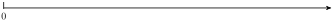
\includegraphics[width=\linewidth]{images/sw-1-3-4}
\end{sbspanel}%
\end{sidebyside}%
\item{}On your axis, plot 250,000 and 472,600.%
\end{enumerate}
%
\end{divisionexercise}%
\begin{divisionexercise}{6}{}{}{g:exercise:idm46056771999536}%
%
\begin{enumerate}[label=\alph*]
\item{}Label an axis in increments of 0.5 from 0 to 5.%
\begin{sidebyside}{1}{0.15}{0.15}{0}%
\begin{sbspanel}{0.7}%
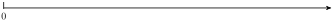
\includegraphics[width=\linewidth]{images/sw-1-3-4}
\end{sbspanel}%
\end{sidebyside}%
\item{}On the axis in part (a), plot 1.3 and 3.77.%
\end{enumerate}
%
\end{divisionexercise}%
\end{exercises-subsubsection}
%
%
\typeout{************************************************}
\typeout{Solutions  Answers to Skills Warm-Up}
\typeout{************************************************}
%
\begin{solutions-subsubsection}{Answers to Skills Warm-Up}{}{Answers to Skills Warm-Up}{}{}{g:solutions:idm46056772021408}
\begin{conclusion}{}%
%
\begin{enumerate}[label=\arabic*]
\item{}\(\displaystyle A: 350;~~B: 825\)%
\item{}\(\displaystyle 700;~~1400\)%
\item{}\begin{sidebyside}{1}{0.2}{0.2}{0}%
\begin{sbspanel}{0.6}%
\resizebox{\linewidth}{!}{%
\tikzset{%
}
\begin{tikzpicture} 
\draw[black,thick, ->, >=stealth'] (0,0)--(11,0);
 \draw[black, thick] (0,.3) --++(0,-.35)  node[below]   {0};
 \draw[black, thick] (10,.3) --++(0,-.35)  node[below]   {10,000};
\foreach \x [evaluate=\x as \xi using int(1000*\x)] in {5/2,5,15/2} \draw[black,thick] (\x,.2) --++(0,-.2) node[below, yshift=-2, scale=.8]{\xi};
\foreach \x [evaluate=\x as \xi using int(1000*\x)]  in {1.25, 3.75, 6.25, 8.75} \draw[black,thick] (\x,.15) --++(0,-.15) node[below, yshift=-2, scale=.8]{\xi};
\filldraw[blue] (1.4,0) circle (1mm) node[above, yshift=4, scale=.9] {1400};
\filldraw[blue] (8.35,0) circle (1mm) node[above, yshift=4, scale=.9] {8350};
\end{tikzpicture}
}%
\end{sbspanel}%
\end{sidebyside}%
%
\item{}\begin{sidebyside}{1}{0.15}{0.15}{0}%
\begin{sbspanel}{0.7}%
\resizebox{\linewidth}{!}{%
\tikzset{%
}
\begin{tikzpicture}  [scale=.7]
\draw[black,thick, ->, >=stealth'] (0,0)--(16.5,0);
\draw[black, thick] (0,.3) --++(0,-.35)  node[below]   {0};
\foreach \x [evaluate=\x as \xi using int(50*\x)]  in {1,2,...,16} \draw[black,thick] (\x,.15) --++(0,-.15) node[below, yshift=-2, scale=.8]{\xi};
\filldraw[blue] (2.64,0) circle (1mm) node[above, yshift=4, scale=.9] {132};
\filldraw[blue] (12.28,0) circle (1mm) node[above, yshift=4, scale=.9] {614};
\end{tikzpicture}
}%
\end{sbspanel}%
\end{sidebyside}%
%
\item{}\begin{sidebyside}{1}{0.15}{0.15}{0}%
\begin{sbspanel}{0.7}%
\resizebox{\linewidth}{!}{%
\tikzset{%
}
\begin{tikzpicture}  [scale=.7]
\draw[black,thick, ->, >=stealth'] (0,0)--(16.5,0);
\draw[black, thick] (0,.3) --++(0,-.35)  node[below]   {0};
\foreach \x [evaluate=\x as \xi using int(40*\x)]  in {1,2,...,15} \draw[black,thick] (\x,.15) --++(0,-.15) node[below, yshift=-2, scale=.8]{\xi};
\filldraw[blue] (6.25,0) circle (1mm) node[above, yshift=4, scale=.9] {250};
\filldraw[blue] (11.815,0) circle (1mm) node[above, yshift=4, scale=.9] {472.6};
\end{tikzpicture}
}%
\end{sbspanel}%
\end{sidebyside}%
%
\item{}\begin{sidebyside}{1}{0.15}{0.15}{0}%
\begin{sbspanel}{0.7}%
\resizebox{\linewidth}{!}{%
\tikzset{%
}
\begin{tikzpicture}  [scale=.7]
\draw[black,thick, ->, >=stealth'] (0,0)--(16.5,0);
\draw[black, thick] (0,.3) --++(0,-.35)  node[below]   {0};
\foreach \x [evaluate=\x as \xi using int(\x/3)]  in {3,6,...,15} \draw[black,thick] (\x,.15) --++(0,-.15) node[below, yshift=-2, scale=.8]{\xi};
\foreach \x [evaluate=\x as \xi using int(\x/3)]  in {1.5,4.5,...,13.5} \draw[black,thick] (\x,.15) --++(0,-.15) node[below, yshift=-2, scale=.8]{\xi.5};
\filldraw[blue] (3.9,0) circle (1mm) node[above, yshift=4, scale=.9] {1.3};
\filldraw[blue] (11.31,0) circle (1mm) node[above, yshift=4, scale=.9] {3.77};
\end{tikzpicture}
}%
\end{sbspanel}%
\end{sidebyside}%
%
\end{enumerate}
%
\end{conclusion}%
\end{solutions-subsubsection}
\end{subsectionptx}
%
%
\typeout{************************************************}
\typeout{Subsection  Lesson}
\typeout{************************************************}
%
\begin{subsectionptx}{Lesson}{}{Lesson}{}{}{g:subsection:idm46056772123136}
\begin{introduction}{}%
\begin{activity}{Making a Graph.}{g:activity:idm46056772127104}%
\begin{assemblage}{To graph an equation.}{g:assemblage:idm46056772133136}%
%
\begin{enumerate}[label=\arabic*]
\item{}Make a table of values.%
\item{}Choose scales for the axes.%
\item{}Plot the points and connect them with a smooth curve.%
\end{enumerate}
%
\end{assemblage}
%
\begin{enumerate}[label=\arabic*]
\item{}Laura takes her daughter Stefanie berry-picking at a local strawberry farm. Laura can pick three baskets of strawberries in the same time that Stefanie picks one basket.%
\par
%
\begin{enumerate}[label=\alph*]
\item{}Let \(L\) stand for the number of baskets Laura has picked and \(S\) for the number of baskets that Stefanie has picked.  Write an equation relating the variables.%
\item{}Graph the equation.%
\par
Step 1: Make a table of values. Choose some reasonable values for \(S\), such as:%
\begin{sidebyside}{1}{0}{0}{0}%
\begin{sbspanel}{1}%
{\centering%
{\tabularfont%
\begin{tabular}{AcAcAcAcAcAcA}\hrulethick
\(S\)&\(1\)&\(2\)&\(4\)&\(7\)&\(10\)\tabularnewline\hrulethin
\(L\)&\(\hphantom{0000}\)&\(\hphantom{0000}\)&\(\hphantom{0000}\)&\(\hphantom{0000}\)&\(\hphantom{0000}\)\tabularnewline\hrulethin
\end{tabular}
}%
\par}
\end{sbspanel}%
\end{sidebyside}%
\par
Use the equation to find the corresponding values of \(L\). For example, when \(S=\alert{1}\),%
\begin{equation*}
L=\hphantom{0000000000000000}
\end{equation*}
amd when \(S=\alert{2}\),%
\begin{equation*}
L=\hphantom{0000000000000000}
\end{equation*}
%
\par
Complete the table.%
\par
Step 2: Label the horizontal axis with the input variable, and the vertical axis with the output variable. Then label the scales on the axes.%
\par
Step 3: Plot the points in the table and connect them with a smooth curve. The points on this graph lie on a straight line.%
\begin{sidebyside}{1}{0.225}{0.225}{0}%
\begin{sbspanel}{0.55}%
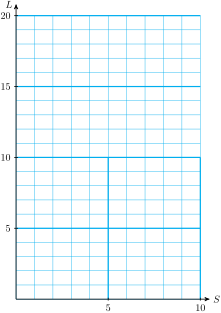
\includegraphics[width=\linewidth]{images/act-1-3-1.png}
\end{sbspanel}%
\end{sidebyside}%
\end{enumerate}
%
\item{}Emily and Megan pledged to walk a total of 12 miles for their school's fundraising walkathon. Let \(E\) stand for the number of miles Emily walks, and \(M\) for the number of miles Megan walks.%
\begin{enumerate}[label=\alph*]
\item{}Write an equation for \(E\) in terms of \(M\).%
\item{}Make a table of values and graph the equation.%
\begin{sidebyside}{1}{0}{0}{0}%
\begin{sbspanel}{1}%
{\centering%
{\tabularfont%
\begin{tabular}{AcAcAcAcAcA}\hrulethick
\(M\)&\(\hphantom{0000}\)&\(\hphantom{0000}\)&\(\hphantom{0000}\)&\(\hphantom{0000}\)\tabularnewline\hrulethin
\(E\)&\(\hphantom{0000}\)&\(\hphantom{0000}\)&\(\hphantom{0000}\)&\(\hphantom{0000}\)\tabularnewline\hrulethin
\end{tabular}
}%
\par}
\end{sbspanel}%
\end{sidebyside}%
\begin{sidebyside}{1}{0.225}{0.225}{0}%
\begin{sbspanel}{0.55}%
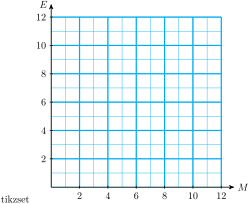
\includegraphics[width=\linewidth]{images/act-1-3-2.png}
\end{sbspanel}%
\end{sidebyside}%
\end{enumerate}
%
\end{enumerate}
%
\end{activity}
\begin{activity}{Choosing Scales for the Axes.}{g:activity:idm46056772458352}%
\index{axis!choosing scale for}%
%
\begin{enumerate}[label=\arabic*]
\item{}Corey's truck holds 20 gallons of gasoline and gets 18 miles to the gallon.%
\begin{enumerate}[label=\alph*]
\item{}Write an equation that relates the distance, \(d\), that Corey can travel to the number of gallons of gas, \(g\), in his truck.%
\item{}Graph the equation.%
\par
Step 1: Make a table of values. Choose values of \(g\) between 0 and 20, because Corey's truck holds 20 gallons of gas. Use the equation to calculate the values of \(d\).%
\begin{sidebyside}{1}{0}{0}{0}%
\begin{sbspanel}{1}%
{\centering%
{\tabularfont%
\begin{tabular}{AcAcAcAcAcAcAcA}\hrulethick
\(g\)&\(2\)&\(5\)&\(8\)&\(10\)&\(15\)&\(20\)\tabularnewline\hrulethin
\(d\)&\(\hphantom{0000}\)&\(\hphantom{0000}\)&\(\hphantom{0000}\)&\(\hphantom{0000}\)&\(\hphantom{0000}\)&\(\hphantom{0000}\)\tabularnewline\hrulethin
\end{tabular}
}%
\par}
\end{sbspanel}%
\end{sidebyside}%
\par
Step 2: Choose scales for the axes: Use 10 grid lines on the horizontal axis. The length of each interval is%
\begin{equation*}
20 \div 10 = \fillin{2.727272727272727} \text{units}
\end{equation*}
so we scale the horizontal axis in intervals of 2. On the vertical axis, we use increments of 25 from 0 to 400, which gives us 16 grid lines.%
\par
Step 3: Plot the points from the table of values. You will need to estimate the location of some of the points between tick marks.%
\begin{sidebyside}{1}{0.225}{0.225}{0}%
\begin{sbspanel}{0.55}%
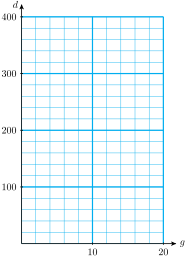
\includegraphics[width=\linewidth]{images/act-1-3-3.png}
\end{sbspanel}%
\end{sidebyside}%
\end{enumerate}
%
\item{}The Harris Aircraft company gave all its employees a 5\% raise.%
\begin{enumerate}[label=\alph*]
\item{}Write an equation that expresses each employee's raise, \(R\), in terms of his or her present salary, \(S\).%
\item{}Graph the equation.%
\par
Step 1: Complete a table of values.%
\begin{sidebyside}{1}{0}{0}{0}%
\begin{sbspanel}{1}%
{\centering%
{\tabularfont%
\begin{tabular}{AcAcAcAcAcA}\hrulethick
\(S\)&\(18,000\)&\(24,000\)&\(32,000\)&\(36,000\)\tabularnewline\hrulethin
\(R\)&\(\hphantom{0000}\)&\(\hphantom{0000}\)&\(\hphantom{0000}\)&\(\hphantom{0000}\)\tabularnewline\hrulethin
\end{tabular}
}%
\par}
\end{sbspanel}%
\end{sidebyside}%
\par
Step 2: Choose scales for the axes and label them. (What are the largest values of \(S\) and \(R\) in your table?)%
\par
Step 3: Plot the points and draw the graph.%
\begin{sidebyside}{1}{0.2}{0.2}{0}%
\begin{sbspanel}{0.6}%
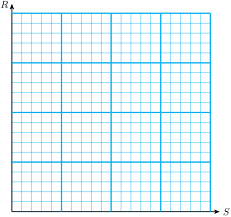
\includegraphics[width=\linewidth]{images/act-1-3-4.png}
\end{sbspanel}%
\end{sidebyside}%
\end{enumerate}
%
\end{enumerate}
%
\end{activity}
\begin{activity}{Using a Graph.}{g:activity:idm46056772628912}%
The Reedville City Council voted that 35\% of the town's budget should be allotted to education.%
\begin{enumerate}[label=\alph*]
\item{}Write an equation for the amount budgeted for education, \(s\), in terms of the total budget, \(b\).%
\par
Use your equation to answer the following questions:%
\item{}If Reedville's total budget for next year is \textdollar{}1,800,000, how much will be allotted for education?%
\item{}If Reedville spent \textdollar{}875,000 on education last year, what was its total budget?%
\end{enumerate}
%
\par
Here is a graph of the equation from part (a).  Both axes of the graph are scaled in thousands of dollars.  Use the graph to estimate the answers to the parts (b) and (c).  Show directly on the graph how you obtained your estimates.%
\begin{sidebyside}{1}{0.225}{0.225}{0}%
\begin{sbspanel}{0.55}%
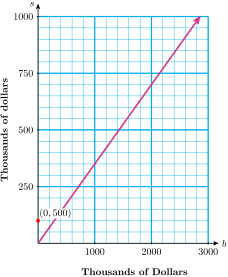
\includegraphics[width=\linewidth]{images/act-1-3-5.png}
\end{sbspanel}%
\end{sidebyside}%
\par
Estimates:  (b) \fillin{8.181818181818182}%
\par
\(\hphantom{000000000}\) (c) \fillin{8.181818181818182}%
\end{activity}
\end{introduction}%
%
%
\typeout{************************************************}
\typeout{Subsubsection  Wrap-Up}
\typeout{************************************************}
%
\begin{subsubsectionptx}{Wrap-Up}{}{Wrap-Up}{}{}{g:subsubsection:idm46056772680944}
\begin{objectives}{Objectives}{g:objectives:idm46056772689216}
In this Lesson we practiced the following skills:%
%
\begin{itemize}[label=\textbullet]
\item{}Making a table of values%
\item{}Choosing scales for the axes%
\item{}Plotting points and drawing a curve%
\item{}Using a graph to evaluate an expression or solve an equation%
\end{itemize}
\end{objectives}
Questions to answer before the Homework Preview.%
\begin{outcomes}{Questions}{g:outcomes:idm46056772708976}
%
\begin{enumerate}[label=\arabic*]
\item{}If you graph the equation \(Q=M+12\), which variable goes on the horizontal axis?%
\item{}If the output values range from 0 to 6000, what would be a good interval to use for the scale on the vertical axis?%
\item{}In Activity 3b, did we evaluate an expression or solve an equation?%
\end{enumerate}
\end{outcomes}
\end{subsubsectionptx}
\end{subsectionptx}
%
%
\typeout{************************************************}
\typeout{Subsection  Homework Preview}
\typeout{************************************************}
%
\begin{subsectionptx}{Homework Preview}{}{Homework Preview}{}{}{g:subsection:idm46056772724384}
Here are exercises to try before the end of the class meeting.%
%
%
\typeout{************************************************}
\typeout{Exercises  Exercises}
\typeout{************************************************}
%
\begin{exercises-subsubsection}{Exercises}{}{Exercises}{}{}{g:exercises:idm46056772734384}
\begin{divisionexercise}{1}{}{}{g:exercise:idm46056772734960}%
Draw axes and label both scales by 5's, from 0 to 30.%
\end{divisionexercise}%
\begin{divisionexercise}{2}{}{}{g:exercise:idm46056772744896}%
Draw axes and label the horizontal scale by 25's, fom 0 to 200, and the vertical scale by 200's, from 0 to 3000.%
\end{divisionexercise}%
\begin{divisionexercise}{3}{}{}{g:exercise:idm46056772751648}%
\begin{sidebyside}{2}{0.0125}{0.0125}{0.025}%
\begin{sbspanel}{0.55}%
%
\begin{enumerate}[label=\alph*]
\item{}What interval does each grid line represent on the horizontal axis? On the vertical axis?%
\item{}Plot the followng points on the grid:%
\begin{equation*}
(0,500),~(20,1750),~(40,250)
\end{equation*}
%
\end{enumerate}
%
\end{sbspanel}%
\begin{sbspanel}{0.4}%
\includegraphics[width=\linewidth]{images/pre-1-3-1.png}
\end{sbspanel}%
\end{sidebyside}%
\end{divisionexercise}%
\begin{divisionexercise}{4}{}{}{g:exercise:idm46056772783056}%
\begin{sidebyside}{2}{0.025}{0.025}{0.05}%
\begin{sbspanel}{0.55}%
%
\begin{enumerate}[label=\alph*]
\item{}What interval does each grid line represent on the horizontal axis? On the vertical axis?%
\item{}Find the coordinates of each point.%
\end{enumerate}
%
\end{sbspanel}%
\begin{sbspanel}{0.35}%
\includegraphics[width=\linewidth]{images/pre-1-3-2.png}
\end{sbspanel}%
\end{sidebyside}%
\end{divisionexercise}%
\end{exercises-subsubsection}
%
%
\typeout{************************************************}
\typeout{Solutions  Answers to Homework Preview}
\typeout{************************************************}
%
\begin{solutions-subsubsection}{Answers to Homework Preview}{}{Answers to Homework Preview}{}{}{g:solutions:idm46056772809072}
\begin{conclusion}{}%
%
\begin{enumerate}[label=\arabic*]
\item{}\begin{sidebyside}{1}{0.35}{0.35}{0}%
\begin{sbspanel}{0.3}%
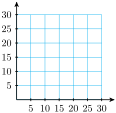
\includegraphics[width=\linewidth]{images/pre-1-3-3.png}
\end{sbspanel}%
\end{sidebyside}%
%
\item{}\begin{sidebyside}{1}{0.35}{0.35}{0}%
\begin{sbspanel}{0.3}%
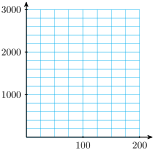
\includegraphics[width=\linewidth]{images/pre-1-3-4.png}
\end{sbspanel}%
\end{sidebyside}%
%
\item{}a.  horizontal: 5; vertical: 250%
\begin{sidebyside}{1}{0.325}{0.325}{0}%
\begin{sbspanel}{0.35}%
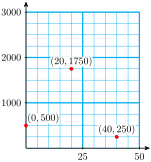
\includegraphics[width=\linewidth]{images/pre-1-3-5.png}
\end{sbspanel}%
\end{sidebyside}%
\item{}a. horizontal: 0.2; vertical: 20%
\par
b. \(A(0.2,160),~B(0.6,60),~C(1.4,120)\)%
\end{enumerate}
%
\end{conclusion}%
\end{solutions-subsubsection}
\end{subsectionptx}
%
%
\typeout{************************************************}
\typeout{Exercises  Homework 1.3}
\typeout{************************************************}
%
\begin{exercises-subsection}{Homework 1.3}{}{Homework 1.3}{}{}{g:exercises:idm46056772855952}
\par\medskip\noindent%
%
For Problems 1\textendash{}2, decide whether the ordered pairs are solutions of the equation whose graph is shown.%
\begin{exercisegroupcol}{2}
\begin{divisionexerciseegcol}{1}{}{}{g:exercise:idm46056772868672}%
%
\begin{multicols}{2}
\begin{enumerate}[label=\alph*]
\item{}\(\displaystyle (6.5,3)\)%
\item{}\(\displaystyle (0,3.5)\)%
\item{}\(\displaystyle (8,2)\)%
\item{}\(\displaystyle (4.5,1)\)%
\end{enumerate}
\end{multicols}
%
\begin{sidebyside}{1}{0.15}{0.15}{0}%
\begin{sbspanel}{0.7}%
\resizebox{\linewidth}{!}{%
\tikzset{%
}
\begin{tikzpicture} [scale=.55]
\draw[cyan!60!white] (0,0) grid[step=1/2] (7,10);
\draw[black,thick,->,>=stealth'] (0,0)--(7.5,0) node[right]{$t$};
\draw[black,thick,->,>=stealth'] (0,0)--(0,10.8)node[left]{$h$};

\foreach \x  in {3,6} {
  \draw[cyan!60!white,ultra thick] (\x,0)--++(0,10);
  \draw[black,thick] (\x,.1)--++(0,-.2) node[below, fill=white, inner sep=1, yshift=-2]{\x};
}
\foreach \x in {5,10} {
  \draw[cyan!60!white,ultra thick] (0,\x)--++(7,0);
  \draw[black,thick] (.1,\x)--++(-.2,0) node[left, fill=white, inner sep=1, xshift=-2]{\x};
}
\draw[magenta!90!black,very thick, ->, >=stealth'] (0,3.5) -- (6.5,10);
\end{tikzpicture}
}%
\end{sbspanel}%
\end{sidebyside}%
\end{divisionexerciseegcol}%
\begin{divisionexerciseegcol}{2}{}{}{g:exercise:idm46056785105584}%
%
\begin{multicols}{2}
\begin{enumerate}[label=\alph*]
\item{}\(\displaystyle (2,6)\)%
\item{}\(\displaystyle (4,2)\)%
\item{}\(\displaystyle (10,0)\)%
\item{}\(\displaystyle (11,7)\)%
\end{enumerate}
\end{multicols}
%
\begin{sidebyside}{1}{0.15}{0.15}{0}%
\begin{sbspanel}{0.7}%
\resizebox{\linewidth}{!}{%
\tikzset{%
}
\begin{tikzpicture} [scale=.33]
\draw[cyan!60!white] (0,0) grid (10,15);
\draw[black,thick,->,>=stealth'] (0,0)--(11.5,0) node[right]{$p$};
\draw[black,thick,->,>=stealth'] (0,0)--(0,16.7)node[left]{$m$};

\foreach \x  in {5,10} {
  \draw[cyan!60!white,ultra thick] (\x,0)--++(0,15);
  \draw[black,thick] (\x,.1)--++(0,-.2) node[below, fill=white, inner sep=1, yshift=-2]{\x};
}
\foreach \x in {5,10,15} {
  \draw[cyan!60!white,ultra thick] (0,\x)--++(10,0);
  \draw[black,thick] (.1,\x)--++(-.2,0) node[left, fill=white, inner sep=1, xshift=-2]{\x};
}
\draw[samples=65,domain={4-sqrt(13):4+sqrt(13)},smooth,variable=\x,magenta!90!black,very thick, <->, >=stealth'] plot ({\x},{2+(\x-4)^2});
\end{tikzpicture}
}%
\end{sbspanel}%
\end{sidebyside}%
\end{divisionexerciseegcol}%
\end{exercisegroupcol}
\par\medskip\noindent
\par\medskip\noindent%
%
For Problems 3\textendash{}6, decide whether the ordered pairs are solutions of the given equation.%
\begin{exercisegroupcol}{2}
\begin{divisionexerciseegcol}{3}{}{}{g:exercise:idm46056770765520}%
\(y=\dfrac{3}{4}x\)%
\begin{multicols}{2}
\begin{enumerate}[label=\alph*]
\item{}\(\displaystyle (8,6)\)%
\item{}\(\displaystyle (12,16)\)%
\item{}\(\displaystyle (2,3)\)%
\item{}\(\displaystyle (6,\dfrac{9}{2})\)%
\end{enumerate}
\end{multicols}
%
\end{divisionexerciseegcol}%
\begin{divisionexerciseegcol}{4}{}{}{g:exercise:idm46056770760400}%
\(y=\dfrac{x}{2.5}\)%
\begin{multicols}{2}
\begin{enumerate}[label=\alph*]
\item{}\(\displaystyle (1,2.5)\)%
\item{}\(\displaystyle (25,10)\)%
\item{}\(\displaystyle (5,2)\)%
\item{}\(\displaystyle (8,20)\)%
\end{enumerate}
\end{multicols}
%
\end{divisionexerciseegcol}%
\begin{divisionexerciseegcol}{5}{}{}{g:exercise:idm46056772983104}%
\(w=z-1.8\)%
\begin{multicols}{2}
\begin{enumerate}[label=\alph*]
\item{}\(\displaystyle (10, 8.8)\)%
\item{}\(\displaystyle (6,7.8)\)%
\item{}\(\displaystyle (2,\dfrac{1}{5})\)%
\item{}\(\displaystyle (9.2,7.4)\)%
\end{enumerate}
\end{multicols}
%
\end{divisionexerciseegcol}%
\begin{divisionexerciseegcol}{6}{}{}{g:exercise:idm46056784872960}%
\(w=120-z\)%
\begin{multicols}{2}
\begin{enumerate}[label=\alph*]
\item{}\(\displaystyle (0, 120)\)%
\item{}\(\displaystyle (65,55)\)%
\item{}\(\displaystyle (150,30)\)%
\item{}\(\displaystyle (9.6,2.4)\)%
\end{enumerate}
\end{multicols}
%
\end{divisionexerciseegcol}%
\end{exercisegroupcol}
\par\medskip\noindent
\par\medskip\noindent%
%
For Problems 7\textendash{}8, state the interval that each grid line represents on the horizontal and vertical axes.%
\begin{exercisegroupcol}{2}
\begin{divisionexerciseegcol}{7}{}{}{g:exercise:idm46056772329952}%
\begin{sidebyside}{1}{0.15}{0.15}{0}%
\begin{sbspanel}{0.7}%
\resizebox{\linewidth}{!}{%
\tikzset{%
}
\begin{tikzpicture} [scale=2]
\draw[cyan] (0,0) grid[xstep=1/4, ystep=1/5] (2,2);
\draw[black,thick, ->, >=stealth'] (0,0)--(2.2,0);
\draw[black,thick, ->, >=stealth'] (0,0)--(0,2.2);
\foreach \x  in  {1,2} {
 \draw[cyan, very thick] (\x,.0) --++(0,2);
 \draw[black, thick] (\x,.05) --++(0,-.1)  node[below] {\x};
}
\foreach \y [evaluate=\y as \yi using int( 20* \y )]  in  {1,2} {
 \draw[cyan, very thick] (0,\y) --++(2,0);
 \draw[black, thick] (.05,\y) --++(-.1,0)  node[left]   {\yi};
}
\end{tikzpicture}
}%
\end{sbspanel}%
\end{sidebyside}%
\end{divisionexerciseegcol}%
\begin{divisionexerciseegcol}{8}{}{}{g:exercise:idm46056773358816}%
\begin{sidebyside}{1}{0.15}{0.15}{0}%
\begin{sbspanel}{0.7}%
\resizebox{\linewidth}{!}{%
\tikzset{%
}
\begin{tikzpicture} [scale=2]
\draw[cyan] (0,0) grid[xstep=1/5, ystep=1/4] (2,3/2);
\draw[black,thick, ->, >=stealth'] (0,0)--(2.2,0);
\draw[black,thick, ->, >=stealth'] (0,0)--(0,1.7);
\foreach \x [evaluate=\x as \xi using int( 250* \x )]  in  {1,2} {
 \draw[cyan, very thick] (\x,.0) --++(0,1.5);
 \draw[black, thick] (\x,.05) --++(0,-.1)  node[below] {\xi};
}
\foreach \y [evaluate=\y as \yi using int( 2* \y )]  in  {1} {
 \draw[cyan, very thick] (0,\y) --++(2,0);
 \draw[black, thick] (.05,\y) --++(-.1,0)  node[left]   {\yi};
}
\end{tikzpicture}
}%
\end{sbspanel}%
\end{sidebyside}%
\end{divisionexerciseegcol}%
\end{exercisegroupcol}
\par\medskip\noindent
\par\medskip\noindent%
%
For the graphs in Problems 9\textendash{}10,%
\begin{enumerate}[label=\alph*]
\item{}Fill in the table with the correct coordinates. Choose your own points to complete the table.%
\item{}Look for a pattern in your table, and write an equation for the second variable in terms of the first variable.%
\end{enumerate}
%
\begin{exercisegroupcol}{2}
\begin{divisionexerciseegcol}{9}{}{}{g:exercise:idm46056773406736}%
\begin{sidebyside}{1}{0}{0}{0}%
\begin{sbspanel}{1}%
{\centering%
{\tabularfont%
\begin{tabular}{AcAcAcAcAcAcAcAcA}\hrulethick
\(x\)&\(\hphantom{00}\)&\(2\)&\(5\)&\(\hphantom{00}\)&\(10\)&\(\hphantom{00}\)&\(\hphantom{00}\)\tabularnewline\hrulethin
\(y\)&\(16\)&\(\hphantom{00}\)&\(\hphantom{00}\)&\(10\)&\(\hphantom{00}\)&\(\hphantom{00}\)&\(\hphantom{00}\)\tabularnewline\hrulethin
\end{tabular}
}%
\par}
\end{sbspanel}%
\end{sidebyside}%
\begin{sidebyside}{1}{0.1}{0.1}{0}%
\begin{sbspanel}{0.8}%
\resizebox{\linewidth}{!}{%
\tikzset{%
}
\begin{tikzpicture} [scale=.25]
\draw[cyan] (0,0) grid (17,17);
\draw[black,thick, ->, >=stealth'] (0,0)--(18.5,0) node[right]{$x$};
\draw[black,thick, ->, >=stealth'] (0,0)--(0,19) node[left]{$y$};
\foreach \x  in  {5,10,15} {
 \draw[cyan, very thick] (\x,.0) --++(0,17);
 \draw[black, thick] (\x,.1) --++(0,-.2)  node[below] {\x};
}
\foreach \y in  {5,10,15} {
 \draw[cyan, very thick] (0,\y) --++(17,0);
 \draw[black, thick] (.1,\y) --++(-.2,0)  node[left]   {\y};
}
\draw[red,very thick](0,16)--(16,0);
\end{tikzpicture}
}%
\end{sbspanel}%
\end{sidebyside}%
\end{divisionexerciseegcol}%
\begin{divisionexerciseegcol}{10}{}{}{g:exercise:idm46056773583968}%
\begin{sidebyside}{1}{0}{0}{0}%
\begin{sbspanel}{1}%
{\centering%
{\tabularfont%
\begin{tabular}{AcAcAcAcAcAcAcAcA}\hrulethick
\(x\)&\(0\)&\(1\)&\(\hphantom{00}\)&\(\hphantom{00}\)&\(7\)&\(\hphantom{00}\)&\(\hphantom{00}\)\tabularnewline\hrulethin
\(y\)&\(\hphantom{00}\)&\(\hphantom{00}\)&\(16\)&\(20\)&\(\hphantom{00}\)&\(\hphantom{00}\)&\(\hphantom{00}\)\tabularnewline\hrulethin
\end{tabular}
}%
\par}
\end{sbspanel}%
\end{sidebyside}%
\begin{sidebyside}{1}{0.1}{0.1}{0}%
\begin{sbspanel}{0.8}%
\resizebox{\linewidth}{!}{%
\tikzset{%
}
\begin{tikzpicture} [scale=.4]5
\draw[cyan] (0,0) grid (10,10);
\draw[black,thick, ->, >=stealth'] (0,0)--(11,0) node[right]{$x$};
\draw[black,thick, ->, >=stealth'] (0,0)--(0,11.5) node[left]{$y$};
\foreach \x  in  {5,10} {
 \draw[cyan, very thick] (\x,.0) --++(0,10);
 \draw[black, thick] (\x,.08) --++(0,-.16)  node[below] {\x};
}
\foreach \y [evaluate=\y as \yi using int( 4* \y )] in  {2,4,...,10} {
 \draw[cyan, very thick] (0,\y) --++(10,0);
 \draw[black, thick] (.08,\y) --++(-.16,0)  node[left]   {\yi};
}
\draw[red,very thick, ->, >=stealth'](0,0)--(10,10);
\end{tikzpicture}
}%
\end{sbspanel}%
\end{sidebyside}%
\end{divisionexerciseegcol}%
\end{exercisegroupcol}
\par\medskip\noindent
\par\medskip\noindent%
%
For Problems 11\textendash{}14, choose the equation that describes the graph. (A graph might have more than one equation.)%
\begin{multicols}{3}
\begin{enumerate}[label=\alph*]
\item{}\(\displaystyle y=150-x\)%
\item{}\(\displaystyle y=15-x\)%
\item{}\(\displaystyle y=0.2x\)%
\item{}\(\displaystyle y=\dfrac{x}{60}\)%
\item{}\(\displaystyle y=\dfrac{x}{5}\)%
\item{}\(\displaystyle y=15+x\)%
\item{}\(\displaystyle y=\dfrac{60}{x}\)%
\item{}\(\displaystyle y=5x\)%
\end{enumerate}
\end{multicols}
%
\begin{exercisegroupcol}{2}
\begin{divisionexerciseegcol}{11}{}{}{g:exercise:idm46056773725104}%
\begin{sidebyside}{1}{0.15}{0.15}{0}%
\begin{sbspanel}{0.7}%
\resizebox{\linewidth}{!}{%
\tikzset{%
}
\begin{tikzpicture} [xscale=.16, yscale=.10]
\draw[cyan] (0,0) grid[step=5] (20,40);
\draw[black,thick, ->, >=stealth'] (0,0)--(23,0) node[right]{$x$};
\draw[black,thick, ->, >=stealth'] (0,0)--(0,44) node[left]{$y$};
\foreach \x  in  {5,10,15,20} {
 \draw[cyan, very thick] (\x,.0) --++(0,40);
 \draw[black, thick] (\x,.8) --++(0,-1.6)  node[below] {\x};
}
\foreach \y in  {10,20,30,40} {
 \draw[cyan, very thick] (0,\y) --++(20,0);
 \draw[black, thick] (.6,\y) --++(-1.2,0)  node[left]   {\y};
}
\draw[red,very thick, ->, >=stealth'](0,15)--(20,35);
\end{tikzpicture}
}%
\end{sbspanel}%
\end{sidebyside}%
\end{divisionexerciseegcol}%
\begin{divisionexerciseegcol}{12}{}{}{g:exercise:idm46056773737520}%
\begin{sidebyside}{1}{0.1}{0.1}{0}%
\begin{sbspanel}{0.8}%
\resizebox{\linewidth}{!}{%
\tikzset{%
}
\begin{tikzpicture} [yscale=.03]
\draw[cyan] (0,0) grid[ystep=10] (5,150);
\draw[black,thick, ->, >=stealth'] (0,0)--(5.4,0) node[right]{$x$};
\draw[black,thick, ->, >=stealth'] (0,0)--(0,170) node[left]{$y$};
\foreach \x  in  {1,2,3,4,5} {
 \draw[cyan, very thick] (\x,.0) --++(0,150);
 \draw[black, thick] (\x,1) --++(0,-2)  node[below] {\x};
}
\foreach \y in  {50,100, 150} {
 \draw[cyan, very thick] (0,\y) --++(5,0);
 \draw[black, thick] (.08,\y) --++(-.16,0)  node[left]   {\y};
}
\draw[samples=65,domain=2/5:5,smooth,variable=\x,red,very thick, <->, >=stealth'] plot ({\x},{60/\x)});
\end{tikzpicture}
}%
\end{sbspanel}%
\end{sidebyside}%
\end{divisionexerciseegcol}%
\begin{divisionexerciseegcol}{13}{}{}{g:exercise:idm46056773758400}%
\begin{sidebyside}{1}{0.1}{0.1}{0}%
\begin{sbspanel}{0.8}%
\resizebox{\linewidth}{!}{%
\tikzset{%
}
\begin{tikzpicture} [xscale=.45,yscale=1.6]
\draw[cyan] (0,0) grid[ystep=1/5] (10,2.4);
\draw[black,thick, ->, >=stealth'] (0,0)--(10.8,0) node[right]{$x$};
\draw[black,thick, ->, >=stealth'] (0,0)--(0,2.6) node[left]{$y$};
\foreach \x  in  {5,10} {
 \draw[cyan, very thick] (\x,.0) --++(0,2.4);
 \draw[black, thick] (\x,.06) --++(0,-.12)  node[below] {\x};
}
\foreach \y in  {1,2} {
 \draw[cyan, very thick] (0,\y) --++(10,0);
 \draw[black, thick] (.1,\y) --++(-.2,0)  node[left]   {\y};
}
\draw[red,very thick, ->, >=stealth'] (0,0)--(10,2);
\end{tikzpicture}
}%
\end{sbspanel}%
\end{sidebyside}%
\end{divisionexerciseegcol}%
\begin{divisionexerciseegcol}{14}{}{}{g:exercise:idm46056773785328}%
\begin{sidebyside}{1}{0.1}{0.1}{0}%
\begin{sbspanel}{0.8}%
\resizebox{\linewidth}{!}{%
\tikzset{%
}
\begin{tikzpicture} [scale=.3]
\draw[cyan] (0,0) grid (15,15);
\draw[black,thick, ->, >=stealth'] (0,0)--(16.5,0) node[right]{$x$};
\draw[black,thick, ->, >=stealth'] (0,0)--(0,17) node[left]{$y$};
\foreach \x  in  {5,10,15} {
 \draw[cyan, very thick] (\x,.0) --++(0,15);
 \draw[black, thick] (\x,.1) --++(0,-.2)  node[below] {\x};
}
\foreach \y in  {5,10,15} {
 \draw[cyan, very thick] (0,\y) --++(15,0);
 \draw[black, thick] (.1,\y) --++(-.2,0)  node[left]   {\y};
}
\draw[red,very thick](0,15)--(15,0);
\end{tikzpicture}
}%
\end{sbspanel}%
\end{sidebyside}%
\end{divisionexerciseegcol}%
\end{exercisegroupcol}
\par\medskip\noindent
\par\medskip\noindent%
%
Use the three steps in the Lesson to make the graphs in Problems 15\textendash{}17.%
\begin{exercisegroup}
\begin{divisionexerciseeg}{15}{}{}{g:exercise:idm46056784573984}%
The college Bookstore charges a 25\% markup over wholesale prices. If the wholesale price of a book is \(w\) dollars, the bookstore's price \(p\) is given by%
\begin{equation*}
p=1.25w
\end{equation*}
%
\begin{enumerate}[label=\alph*]
\item{}How much does the bookstore charge for a book whose wholesale price is \textdollar{}28?%
\item{}Evaluate the formula to find the bookstore's price for various books.%
\begin{sidebyside}{1}{0}{0}{0}%
\begin{sbspanel}{1}%
{\centering%
{\tabularfont%
\begin{tabular}{AcAcAcAcAcAcAcA}\hrulethick
\(w\)&\(12\)&\(16\)&\(20\)&\(30\)&\(36\)&\(40\)\tabularnewline\hrulethin
\(p\)&\(\hphantom{00}\)&\(\hphantom{00}\)&\(\hphantom{00}\)&\(\hphantom{00}\)&\(\hphantom{00}\)&\(\hphantom{00}\)\tabularnewline\hrulethin
\end{tabular}
}%
\par}
\end{sbspanel}%
\end{sidebyside}%
\item{}Plot the values from the table and graph the equation.%
\begin{sidebyside}{1}{0.25}{0.25}{0}%
\begin{sbspanel}{0.5}%
\resizebox{\linewidth}{!}{%
\tikzset{%
}
\begin{tikzpicture} [xscale=.125, yscale=.1]
\draw[cyan] (0,0) grid[xstep=4, ystep=5] (40,50);
\draw[black,thick, ->, >=stealth'] (0,0)--(43,0) node[right]{$w$};
\draw[black,thick, ->, >=stealth'] (0,0)--(0,54) node[left, xshift=1]{$P$};
\foreach \x  in  {8,16,...,40} {
 \draw[black, thick] (\x,0.8) --++(0,-1.6)  node[below] {\x};
}
\foreach \y in  {10, 20, 30, 40,50} {
 \draw[black, thick] (.8,\y) --++(-1.6,0)  node[left]   {\y};
}
\end{tikzpicture}
}%
\end{sbspanel}%
\end{sidebyside}%
\end{enumerate}
%
\end{divisionexerciseeg}%
\begin{divisionexerciseeg}{16}{}{}{g:exercise:idm46056784474896}%
Uncle Ray's diet allows him to eat a total of 1000 calories for lunch and dinner. Let \(L\) stand for the number of calories in Uncle Ray's lunch, and \(D\) for the number of calories in his dinner.%
\begin{enumerate}[label=\alph*]
\item{}Write an equation for \(D\) in terms of \(L\).%
\item{}Complete the table.%
\begin{sidebyside}{1}{0}{0}{0}%
\begin{sbspanel}{1}%
{\centering%
{\tabularfont%
\begin{tabular}{AcAcAcAcAcA}\hrulethick
\(L\)&\(250\)&\(300\)&\(450\)&\(60\)\tabularnewline\hrulethin
\(D\)&\(\hphantom{00}\)&\(\hphantom{00}\)&\(\hphantom{00}\)&\(\hphantom{00}\)\tabularnewline\hrulethin
\end{tabular}
}%
\par}
\end{sbspanel}%
\end{sidebyside}%
\item{}Label the scales on the axes and graph the equation. Use intervals of 100 on both axes.%
\begin{sidebyside}{1}{0.25}{0.25}{0}%
\begin{sbspanel}{0.5}%
\resizebox{\linewidth}{!}{%
\tikzset{%
}
\begin{tikzpicture} [scale=.5]
\draw[cyan] (0,0) grid (10,10);
\draw[black,thick, ->, >=stealth'] (0,0)--(10.5,0) node[right]{$L$};
\draw[black,thick, ->, >=stealth'] (0,0)--(0,10.5) node[left, xshift=1]{$D$};
\foreach \x  in  {1,2,...,10} {
 \draw[black, thick] (\x,0.09) --++(0,-.18);
}
\foreach \y in  {1,2,...,10} {
 \draw[black, thick] (.09,\y) --++(-.18,0);
}
\end{tikzpicture}
}%
\end{sbspanel}%
\end{sidebyside}%
\end{enumerate}
%
\end{divisionexerciseeg}%
\begin{divisionexerciseeg}{17}{}{}{g:exercise:idm46056774077184}%
The Green Co-op plans to divide its profit of \textdollar{}3600 from the sale of environmentally safe products among its members. Let \(m\) stand for the number of members, and \(S\) for the share of the profits each member will receive.%
\begin{enumerate}[label=\alph*]
\item{}Write an equation for \(S\) in terms of \(m\).%
\item{}Complete the table.%
\begin{sidebyside}{1}{0}{0}{0}%
\begin{sbspanel}{1}%
{\centering%
{\tabularfont%
\begin{tabular}{AcAcAcAcAcA}\hrulethick
\(m\)&\(20\)&\(40\)&\(60\)&\(100\)\tabularnewline\hrulethin
\(S\)&\(\hphantom{00}\)&\(\hphantom{00}\)&\(\hphantom{00}\)&\(\hphantom{00}\)\tabularnewline\hrulethin
\end{tabular}
}%
\par}
\end{sbspanel}%
\end{sidebyside}%
\item{}Label the scales on the axes and graph the equation. Use intervals of 20 on the vertical axis.%
\begin{sidebyside}{1}{0.25}{0.25}{0}%
\begin{sbspanel}{0.5}%
\resizebox{\linewidth}{!}{%
\tikzset{%
}
\begin{tikzpicture} [scale=.5]
\draw[cyan] (0,0) grid (10,10);
\draw[black,thick, ->, >=stealth'] (0,0)--(10.5,0) node[right]{$m$};
\draw[black,thick, ->, >=stealth'] (0,0)--(0,10.5) node[left, xshift=1]{$S$};
\foreach \x  in  {1,2,...,10} {
 \draw[black, thick] (\x,0.09) --++(0,-.18);
}
\foreach \y in  {1,2,...,10} {
 \draw[black, thick] (.09,\y) --++(-.18,0);
}
\end{tikzpicture}
}%
\end{sbspanel}%
\end{sidebyside}%
\end{enumerate}
%
\end{divisionexerciseeg}%
\end{exercisegroup}
\par\medskip\noindent
\par\medskip\noindent%
%
For Problems 18\textendash{}19, solve the equation graphically by drawing on the graph. (You may have to estimate some of your solutions.) Then verify your answer by solving algebraically.%
\begin{exercisegroup}
\begin{divisionexerciseeg}{18}{}{}{g:exercise:idm46056784210208}%
The graph of \(k=p-20\) is shown below. Use the graph to solve the equations:%
\begin{multicols}{2}
\begin{enumerate}[label=\alph*]
\item{}\(\displaystyle 90=p-20\)%
\item{}\(\displaystyle p-20=40\)%
\end{enumerate}
\end{multicols}
%
\begin{sidebyside}{1}{0.275}{0.275}{0}%
\begin{sbspanel}{0.45}%
\resizebox{\linewidth}{!}{%
\tikzset{%
}
\begin{tikzpicture} [scale=.04]
\draw[cyan] (0,0) grid[step=10] (150,150);
\draw[black,thick, ->, >=stealth'] (0,0)--(165,0) node[right]{$p$};
\draw[black,thick, ->, >=stealth'] (0,0)--(0,165) node[left]{$k$};
\foreach \x  in  {50,100,150} {
 \draw[cyan, very thick] (\x,.0) --++(0,150);
 \draw[black, thick] (\x,1) --++(0,-2)  node[below] {\x};
}
\foreach \y in  {50,100,150} {
 \draw[cyan, very thick] (0,\y) --++(150,0);
 \draw[black, thick] (1,\y) --++(-2,0)  node[left]   {\y};
}
\draw[red,very thick, ->,>=stealth'](2,0)--(150,120);
\node[fill=white, inner sep=1, text=red] at (110,115) {$k=p-20$};
\end{tikzpicture}
}%
\end{sbspanel}%
\end{sidebyside}%
\end{divisionexerciseeg}%
\begin{divisionexerciseeg}{19}{}{}{g:exercise:idm46056784205184}%
The graph of \(d=18g\) is shown below. Use the graph to solve the equations:%
\begin{multicols}{2}
\begin{enumerate}[label=\alph*]
\item{}\(\displaystyle 250=18g\)%
\item{}\(\displaystyle 18g=210\)%
\end{enumerate}
\end{multicols}
%
\begin{sidebyside}{1}{0.3}{0.3}{0}%
\begin{sbspanel}{0.4}%
\resizebox{\linewidth}{!}{%
\tikzset{%
}
\begin{tikzpicture} [xscale=.2, yscale=.015]
\draw[cyan] (0,0) grid[xstep=2, ystep=20] (20,400);
\draw[black,thick, ->, >=stealth'] (0,0)--(24,0) node[right]{$g$};
\draw[black,thick, ->, >=stealth'] (0,0)--(0,440) node[left]{$d$};
\foreach \x  in  {10,20} {
 \draw[cyan, very thick] (\x,.0) --++(0,400);
 \draw[black, thick] (\x,1) --++(0,-2)  node[below] {\x};
}
\foreach \y in  {100, 200, 300, 400} {
 \draw[cyan, very thick] (0,\y) --++(20,0);
 \draw[black, thick] (.4,\y) --++(-.8,0)  node[left]   {\y};
}
\draw[red,very thick, ->,>=stealth'](0,0)--(20,360);
\node[fill=white, inner sep=1, text=red] at (14,340) {$d=18g$};
\end{tikzpicture}
}%
\end{sbspanel}%
\end{sidebyside}%
\end{divisionexerciseeg}%
\end{exercisegroup}
\par\medskip\noindent
\par\medskip\noindent%
%
For Problems 20\textendash{}21,%
\begin{enumerate}[label=\alph*]
\item{}Give the coordinates of the indicated point.%
\item{}Explain what those coordinates tell us about the problem situation.%
\end{enumerate}
%
\begin{exercisegroup}
\begin{divisionexerciseeg}{20}{}{}{g:exercise:idm46056785119216}%
The graph gives the sales tax, \(T\), in terms of the price \(p\) of an item, where the amounts are in dollars.%
\begin{sidebyside}{1}{0.325}{0.325}{0}%
\begin{sbspanel}{0.35}%
\resizebox{\linewidth}{!}{%
\tikzset{%
}
\begin{tikzpicture} [xscale=.032, yscale=.32]
\draw[cyan] (0,0) grid[xstep=10, ystep=1] (100,10);
\draw[black,thick, ->, >=stealth'] (0,0)--(120,0) node[right]{$p$};
\draw[black,thick, ->, >=stealth'] (0,0)--(0,12) node[left]{$T$};
\foreach \x  in  {50,100} {
 \draw[cyan, very thick] (\x,.0) --++(0,10);
 \draw[black, thick] (\x,.1) --++(0,-.2)  node[below] {\x};
}
\foreach \y in  {5,10} {
 \draw[cyan, very thick] (0,\y) --++(100,0);
 \draw[black, thick] (.01,\y) --++(-.02,0)  node[left] {\y};
}
\draw[red,very thick, ->,>=stealth'](0,0)--(100,8);
\filldraw[red] (50,4) ellipse(2cm and 2mm) node[above left, xshift=-1, yshift=2,fill=white, inner sep=1, text=black] {$A$};
\end{tikzpicture}
}%
\end{sbspanel}%
\end{sidebyside}%
\end{divisionexerciseeg}%
\begin{divisionexerciseeg}{21}{}{}{g:exercise:idm46056785114912}%
The graph gives the weight, \(W\), in ounces of a chocolate bunny that is \(h\) inches tall.%
\begin{sidebyside}{1}{0.325}{0.325}{0}%
\begin{sbspanel}{0.35}%
\resizebox{\linewidth}{!}{%
\tikzset{%
}
\begin{tikzpicture} [xscale=.8, yscale=.2]
\draw[cyan] (0,0) grid[xstep=1, ystep=2] (5,20);
\draw[black,thick, ->, >=stealth'] (0,0)--(5.5,0) node[right]{$h$};
\draw[black,thick, ->, >=stealth'] (0,0)--(0,22.5) node[left]{$W$};
\foreach \x  in  {1,2,3,4,5} {
 \draw[cyan, very thick] (\x,.0) --++(0,20);
 \draw[black, thick] (\x,.1) --++(0,-.2)  node[below] {\x};
}
\foreach \y in  {10,20} {
 \draw[cyan, very thick] (0,\y) --++(5,0);
 \draw[black, thick] (.01,\y) --++(-.02,0)  node[left] {\y};
}
\draw[samples=65,domain=0:{2*10^(1/3)},smooth,variable=\x,red,very thick, ->, >=stealth'] plot ({\x},{(\x^3)/4});
\filldraw[red] (4,16) ellipse(1mm and 4mm) node[above left, xshift=-3, fill=white, inner sep=1, text=black] {$B$};
\end{tikzpicture}
}%
\end{sbspanel}%
\end{sidebyside}%
\end{divisionexerciseeg}%
\end{exercisegroup}
\par\medskip\noindent
\par\medskip\noindent%
%
For Problems 22\textendash{}25, use the formulas in Section 1.2.%
\begin{exercisegroup}
\begin{divisionexerciseeg}{22}{}{}{g:exercise:idm46056783713744}%
%
\begin{enumerate}[label=\alph*]
\item{}Suppose your father loans you \textdollar{}2000 to be repaid with 4\% annual interest when you finish school. Write an equation for the amount of interest \(I\) you will owe after \(t\) years.%
\item{}How much interest will you owe if you finish school in 2 years? In 4 years? In 7 years? Make a table showing your answers as ordered pairs.%
\item{}Use your table to choose appropriate scales for the axes, then plot points and sketch a graph of the equation%
\end{enumerate}
%
\end{divisionexerciseeg}%
\begin{divisionexerciseeg}{23}{}{}{g:exercise:idm46056783711008}%
%
\begin{enumerate}[label=\alph*]
\item{}The Earth Alliance made \textdollar{}6000 in revenue from selling tickets to Earth Day, an event for children. Write an equation for its profit \(P\) in terms of its costs.%
\item{}What was their profit if their costs were \textdollar{}800? \textdollar{}1000? \textdollar{}2500? Make a table showing your answers as ordered pairs.%
\item{}Use your table to choose appropriate scales for the axes, then plot points and sketch a graph of the equation.%
\end{enumerate}
%
\end{divisionexerciseeg}%
\begin{divisionexerciseeg}{24}{}{}{g:exercise:idm46056774382864}%
%
\begin{enumerate}[label=\alph*]
\item{}Edgar's great-aunt plans to put \textdollar{}5000 in a trust for Edgar until he turns 21, three years from now. She has a choice of several different accounts. Write an equation for the amount of interest the money will earn in 3 years if the account pays interest rate \(r\).%
\item{}How much interest will the \textdollar{}5000 earn in an account that pays 8\% interest? 10\% interest? 12\% interest? Make a table showing your answers as ordered pairs.%
\item{}Use your table to choose appropriate scales for the axes, then plot points and sketch a graph of the equation.%
\end{enumerate}
%
\end{divisionexerciseeg}%
\begin{divisionexerciseeg}{25}{}{}{g:exercise:idm46056774395856}%
%
\begin{enumerate}[label=\alph*]
\item{}Delbert keeps track of the total number of points he earns on homework assignments, each of which is worth 30 points. At the end of the semester he has 540 points. Write an equation for Delbert's average homework score in terms of the number of assignments, \(n\).%
\item{}What is Delbert's average score if there were 20 assignments? 25 assignments? 30 assignments? Make a table showing your answers as ordered pairs.%
\item{}Use your table to choose appropriate scales for the axes, then plot points and sketch a graph of the equation.%
\end{enumerate}
%
\end{divisionexerciseeg}%
\end{exercisegroup}
\par\medskip\noindent
\end{exercises-subsection}
\end{sectionptx}
%
%
\typeout{************************************************}
\typeout{Section 1.4 Solving Equations}
\typeout{************************************************}
%
\begin{sectionptx}{Solving Equations}{}{Solving Equations}{}{}{x:section:Solving-Equations}
\index{equation!solution of}%
%
%
\typeout{************************************************}
\typeout{Subsection  What is an Equation?}
\typeout{************************************************}
%
\begin{subsectionptx}{What is an Equation?}{}{What is an Equation?}{}{}{g:subsection:idm46056774472656}
\begin{assemblage}{Equation.}{g:assemblage:idm46056774475968}%
An \terminology{equation} is a statement that two expressions are equal. It may involve one or more variables.%
\end{assemblage}
\begin{example}{}{x:example:Example-1-4-1}%
Liz makes \textdollar{}6 an hour as a tutor in the Math Lab. Her weekly earnings, \(w\), depend on the number of hours she works, \(h\). The equation relating these two variables is%
\begin{equation*}
w=6h
\end{equation*}
If we know the value of \(h\), we can evaluate the expression \(6h\) to find Liz's earnings. For example, if \(h=\alert{7}\), then%
\begin{equation*}
w=6(\alert{7})=42
\end{equation*}
Liz makes \textdollar{}42 for 7 hours of work.%
\end{example}
In the previous Example we used evaluation to find the value of \(w\) when we knew the value of \(h\). What if we know the value of \(w\) and want to find \(h\)? Suppose Liz earned \textdollar{}54 last week. How many hours did she work? To answer this question we substitute \(\alert{54}\) for \(w\), so that the equation becomes%
\begin{equation*}
\alert{54} = 6h
\end{equation*}
Now we have an equation in just one variable. We would like to find the value of \(h\) that makes this equation true.%
\begin{definition}{Solution of Equation.}{g:definition:idm46056774559024}%
\index{equation!solution of}%
\index{solution!of equation}%
\index{solving an equation}%
\index{solving an equation|seealso{equation}}%
A value of the variable that makes an equation true is called a \terminology{solution} of the equation, and the process of finding this value is called \terminology{solving} the equation.%
\end{definition}
\end{subsectionptx}
%
%
\typeout{************************************************}
\typeout{Subsection  Trial and Error}
\typeout{************************************************}
%
\begin{subsectionptx}{Trial and Error}{}{Trial and Error}{}{}{g:subsection:idm46056774593616}
\index{trial and error}%
\begin{introduction}{}%
Some equations are easy enough to solve by trial and error. You can probably see that the solution of the equation \(~54=6h~\) is 9. We can use a table to help us solve a harder equation by trial and error.%
\par
EXERCISE 1. One of Aunt Esther's Chocolate Dream cookies contains 42 calories, so \(d\) cookies contain \(c\) calories, and \(c=42d\). If Albert consumed 546 calories, how many cookies did he eat? Use trial and error to help you solve the equation \(546=42d\).%
\begin{sidebyside}{1}{0}{0}{0}%
\begin{sbspanel}{1}%
{\centering%
{\tabularfont%
\begin{tabular}{AcAcAcAcAcAcAcAcAcAcAcAcA}\hrulethick
\(d\)&\(5\)&\(6\)&\(7\)&\(8\)&\(9\)&\(10\)&\(11\)&\(12\)&\(13\)&\(14\)&\(15\)\tabularnewline\hrulethin
\(c\)&\(\hphantom{00}\)&\(\hphantom{00}\)&\(\hphantom{00}\)&\(\hphantom{00}\)&\(\hphantom{00}\)&\(\hphantom{00}\)&\(\hphantom{00}\)&\(\hphantom{00}\)&\(\hphantom{00}\)&\(\hphantom{00}\)&\(\hphantom{00}\)\tabularnewline\hrulethin
\end{tabular}
}%
\par}
\end{sbspanel}%
\end{sidebyside}%
\par
\(\vphantom{d=13}\)%
\begin{assemblage}{Look Ahead.}{g:assemblage:idm46056777230400}%
Trial and error can be time-consuming, especially for complicated equations! In this section we investigate some algebraic methods for solving equations.%
\end{assemblage}
\end{introduction}%
%
%
\typeout{************************************************}
\typeout{Subsubsection  Reading Questions}
\typeout{************************************************}
%
\begin{subsubsectionptx}{Reading Questions}{}{Reading Questions}{}{}{g:subsubsection:idm46056777241024}
\begin{inlineexercise}{}{g:exercise:idm46056777246512}%
What is an equation?%
\par\smallskip%
\noindent\textbf{\blocktitlefont Answer}.\hypertarget{g:answer:idm46056777256128}{}\quad{}An equation is a statement that two expressions are equal.%
\end{inlineexercise}
\begin{inlineexercise}{}{g:exercise:idm46056777256816}%
What is a solution of an equation?%
\par\smallskip%
\noindent\textbf{\blocktitlefont Answer}.\hypertarget{g:answer:idm46056777260496}{}\quad{}A value of the variable that makes an equation true.%
\end{inlineexercise}
\end{subsubsectionptx}
\end{subsectionptx}
%
%
\typeout{************************************************}
\typeout{Subsection  Inverse Operations}
\typeout{************************************************}
%
\begin{subsectionptx}{Inverse Operations}{}{Inverse Operations}{}{}{g:subsection:idm46056777263568}
\index{inverse operations}%
Instead of relying on trial and error to solve equations, we will use \terminology{inverse operations}. Try the Exercise below.%
\par
EXERCISE 2.%
\begin{align*}
\amp \blert{\text{Choose any number for}~x:} \amp x \amp = ~\rule{1cm}{0.15mm}\\
\amp \blert{\text{Multiply your number by 5}:} \amp 5x \amp = ~\rule{1cm}{0.15mm}\\
\amp \blert{\text{Divide the result by 5}:}  \amp \dfrac{5x}{5} \amp = ~\rule{1cm}{0.15mm}
\end{align*}
Did you end up with your original number? Try multiplying and dividing your number by another number besides 5. Do you still end up with your original number?%
\begin{assemblage}{Inverse Operations.}{g:assemblage:idm46056777283616}%
Multiplication and division are opposite or \terminology{inverse operations}, because each operation undoes the effects of the other.%
\end{assemblage}
EXERCISE 3.%
\begin{align*}
\amp \blert{\text{Choose any number for}~x:} \amp x \amp = ~\rule{1cm}{0.15mm}\\
\amp \blert{\text{Add 4 to your number}:} \amp x+4 \amp = ~\rule{1cm}{0.15mm}\\
\amp \blert{\text{Subtract 4 from the result}:}  \amp x+4-4 \amp = ~\rule{1cm}{0.15mm}
\end{align*}
Did you end up with your original number? Try adding and subtracting another number besides 4. Do you still end up with your original number?%
\begin{assemblage}{More Inverse Operations.}{g:assemblage:idm46056777309504}%
Addition and subtraction are opposite or \terminology{inverse operations}, because each operation undoes the effects of the other.%
\end{assemblage}
We see that the opposite operation for multiplication is division, and the opposite operation for addition is subtraction. Now we can solve the equation in \hyperref[x:example:Example-1-4-1]{Example~{\xreffont\ref{x:example:Example-1-4-1}}}.%
\begin{example}{}{g:example:idm46056777323456}%
Solve the equation \(~54=6h\).%
\par\smallskip%
\noindent\textbf{\blocktitlefont Solution}.\hypertarget{g:solution:idm46056777354448}{}\quad{}We will transform this equation into a new one of the form \(h=k\) (or \(k=h\)), where the number \(k\) is the solution.%
\par
To do this, we must isolate the variable \(h\) on one side of the equals sign. Because \(h\) is multiplied by 6 in this equation, we divide both sides by 6, like this:%
\begin{align*}
\dfrac{54}{\blert{6}} \amp = \dfrac{6h}{\blert{6}} \amp \amp \blert{\text{Divide both sides by 6.}}\\
9 \amp = h
\end{align*}
The solution is 9. Liz worked for 9 hours.%
\end{example}
\begin{assemblage}{Look Closer.}{g:assemblage:idm46056777380736}%
Note that the expression \(\dfrac{6h}{6}\) says "multiply \(h\) by 6, then divide the result by 6," so we end up with \(h\) again.%
\end{assemblage}
In the previous Example, we transformed the equation into a simpler one (namely, \(h=9\)) which tells us the solution. We can use the following operations to transform an equation:%
\begin{assemblage}{To solve an equation algebraically.}{g:assemblage:idm46056777411744}%
%
\begin{enumerate}[label=\arabic*]
\item{}We can add or subtract the same number from both sides.%
\item{}We can multiply or divide both sides by the same number, as long as that number is not zero.%
\end{enumerate}
%
\end{assemblage}
\begin{assemblage}{Look Closer.}{g:assemblage:idm46056777445152}%
Our method for solving equations works because of the \terminology{properties of equality}, one for each of the four arithmetic operations. They are listed below.%
\end{assemblage}
\begin{assemblage}{Addition and Subtraction Properties of Equality.}{g:assemblage:idm46056777450096}%
If the same quantity is added to or subtracted from both sides of an equation, the solution is unchanged. In symbols,%
\begin{equation*}
\blert{\text{If}~~a=b,~~ \text{then}~~a+c=b+c~~\text{and}~~a-c=b-c}
\end{equation*}
%
\end{assemblage}
\begin{assemblage}{Multiplication and Division Properties of Equality.}{g:assemblage:idm46056777466624}%
If both sides of an equation are multiplied or divided by the same nonzero quantity, the solution is unchanged. In symbols,%
\begin{equation*}
\blert{\text{If}~~a=b,~~ \text{then}~~ac=bc~~\text{and}~~\dfrac{a}{c}=\dfrac{b}{c},~~c\not=0}
\end{equation*}
%
\end{assemblage}
Applying any one of these properties to an equation produces an \terminology{equivalent equation}: one with the same solutions as the original equation.%
\end{subsectionptx}
%
%
\typeout{************************************************}
\typeout{Subsection  Solving Equations}
\typeout{************************************************}
%
\begin{subsectionptx}{Solving Equations}{}{Solving Equations}{}{}{g:subsection:idm46056777507760}
\index{equation!solving}%
\begin{introduction}{}%
Now we can solve equations algebraically. We'll start with the simple Example from Section 1.3 about Delbert's and Francine's ages.%
\begin{example}{}{g:example:idm46056777516288}%
Francine is exactly four years older than Delbert, so an equation relating their ages is \(F=D+4\).  How old is Delbert when Francine is 19?%
\par\smallskip%
\noindent\textbf{\blocktitlefont Solution}.\hypertarget{g:solution:idm46056784328528}{}\quad{}We must solve the equation%
\begin{equation*}
19=D+4
\end{equation*}
We see that 4 has been added to the variable, \(D\). To isolate \(D\) on one side of the equals sign, we subtract 4 from both sides of the equation, like this:%
\begin{align*}
19 \amp = D+4 \\
\underline{\blert{-4}} \amp = \underline{~~~\,\blert{-4}} \amp \amp \blert{\text{Note that} ~D+4-4=D}\\
15 \amp = D
\end{align*}
The solution to this equation is 15. You can check that substituting \(\alert{15}\) for \(D\) does make the equation true.%
\begin{align*}
\blert{\text{Check:}}\amp \amp 19 \amp = D+4   \amp \amp \blert{\text{Substitute}~ 15~ \text{for}~D.}\\
\amp \amp 19 \amp =\alert{15} +4 \amp \amp \blert{\text{True:  the solution checks.}}
\end{align*}
%
\end{example}
\begin{assemblage}{Look Ahead.}{g:assemblage:idm46056783842512}%
That last example is easy enough to solve without algebra, but the method will help us with harder problems. Here is a general strategy for solving such equations.%
\end{assemblage}
\begin{assemblage}{To solve an equation algebraically.}{g:assemblage:idm46056777519168}%
%
\begin{enumerate}[label=\arabic*]
\item{}Ask yourself what operation has been performed on the variable.%
\item{}Perform the opposite operation on both sides of the equation in order to isolate the variable.%
\end{enumerate}
%
\end{assemblage}
\end{introduction}%
%
%
\typeout{************************************************}
\typeout{Subsubsection  Reading Questions}
\typeout{************************************************}
%
\begin{subsubsectionptx}{Reading Questions}{}{Reading Questions}{}{}{g:subsubsection:idm46056777518880}
\begin{inlineexercise}{}{g:exercise:idm46056774338432}%
What is the opposite operation for subtraction? For multiplication?%
\par\smallskip%
\noindent\textbf{\blocktitlefont Answer}.\hypertarget{g:answer:idm46056774657472}{}\quad{}Addition, division%
\end{inlineexercise}
\begin{inlineexercise}{}{g:exercise:idm46056774663616}%
What are equivalent equations?%
\par\smallskip%
\noindent\textbf{\blocktitlefont Answer}.\hypertarget{g:answer:idm46056774665680}{}\quad{}Equations with the same solutions.%
\end{inlineexercise}
\end{subsubsectionptx}
\end{subsectionptx}
%
%
\typeout{************************************************}
\typeout{Subsection  Problem Solving with Equations}
\typeout{************************************************}
%
\begin{subsectionptx}{Problem Solving with Equations}{}{Problem Solving with Equations}{}{}{g:subsection:idm46056774676464}
\index{equation!problem solving with}%
\begin{introduction}{}%
Some problems can be solved by applying one of our familiar formulas.%
\begin{example}{}{g:example:idm46056774690352}%
A saving's account at Al's Bank earns 5\% annual interest. Jan's account earned \textdollar{}42.50 in interest last year. What was her balance at the beginning of the year?%
\par\smallskip%
\noindent\textbf{\blocktitlefont Solution}.\hypertarget{g:solution:idm46056774696928}{}\quad{}First, we choose the appropriate formula. This is a problem about interest, so we use the interest formula:%
\begin{equation*}
\blert{I=Prt}
\end{equation*}
Next, we list the values of the variables. (Which variable is unknown?)%
\begin{align*}
I \amp = \alert{42.50} \amp  r \amp = \alert{0.05}\\
P \amp = \text{unknown}   \amp  t \amp = \alert{1}
\end{align*}
We substitute the values into the formula:%
\begin{equation*}
\alert{42.50}=P(\alert{0.05})(\alert{1})
\end{equation*}
Then we solve the equation:%
\begin{align*}
\dfrac{42.50}{0.05} \amp =\dfrac{P(0.05)}{0.05} \amp \amp \blert{\text{Divide both sides by}~0.05.}\\
850 \amp = P 
\end{align*}
Finally, we answer the question in a sentence:%
\begin{equation*}
\blert{\text{Jan's account balance was }\$850 \text{ at the beginning of the year.}}
\end{equation*}
%
\end{example}
Many practical problems can be solved by first writing an equation that describes or \terminology{models} the problem, and then solving the equation. We will use three steps to solve applied problems.%
\begin{assemblage}{Steps for solving an applied problem.}{g:assemblage:idm46056774753680}%
%
\begin{enumerate}[label=\arabic*]
\item{}Identify the unknown quantity and choose a variable to represent it.%
\item{}Find some quantity that can be described in two different ways, and write an equation using the variable to model the problem situation.%
\item{}Solve the equation and answer the question in the problem.%
\end{enumerate}
%
\end{assemblage}
\begin{example}{}{x:example:Example-1-4-5}%
Jerry needs an additional \textdollar{}35 for airfare to New York. The ticket to New York costs \textdollar{}293. How much money does Jerry have?%
\par\smallskip%
\noindent\textbf{\blocktitlefont Solution}.\hypertarget{g:solution:idm46056774790544}{}\quad{}We follow the three steps.%
\begin{enumerate}[label=\arabic*]
\item{}The amount of money Jerry has is unknown.%
\begin{equation*}
\blert{\text{Amount of money Jerry has:}~~m}
\end{equation*}
%
\item{}The airfare to New York can be described in two different ways:%
\begin{equation*}
\begin{alignedat}{5}
\amp \quad m\amp +\amp\quad 35 \amp =\quad \amp ~~ 293{}\\
\amp \,\text{amount }\amp\amp~\text{amount} \amp\amp\text{airfare}  \\
\amp\text{Jerry has }\amp\amp\text{he needs}
\end{alignedat}
\end{equation*}
%
\item{}We solve the equation and answer the question.%
\begin{equation*}
\begin{alignedat}{9}
m \amp{}+ 35\amp \amp{}=  ~293 \amp\amp  \qquad \blert{\text{Subtract 35 from both sides.}}\\
\amp\underline{{}-{}\blert{35}} \amp  \amp\quad \underline{{}-{}\blert{35}}\\
\amp \quad\, m \amp \amp {}= ~258 
\end{alignedat}
\end{equation*}
%
\par
Jerry has \textdollar{}258.%
\end{enumerate}
%
\end{example}
\begin{warning}{}{g:warning:idm46056774855696}%
In Example 5, each side of the equation represents the airfare to New York, not the amount of money Jerry has, which is what we want to find. This is typical of applied problems: the equation does not usually represent the unknown quantity itself, but some related quantity.%
\end{warning}
\begin{assemblage}{Look Ahead.}{g:assemblage:idm46056774860272}%
Although you may be able to solve the problems in this lesson with arithmetic, the important thing is to learn to write the algebraic equation, or model, for the problem. This skill will help you to solve problems that are too difficult to solve with arithmetic alone.%
\end{assemblage}
\end{introduction}%
%
%
\typeout{************************************************}
\typeout{Subsubsection  Reading Questions}
\typeout{************************************************}
%
\begin{subsubsectionptx}{Reading Questions}{}{Reading Questions}{}{}{g:subsubsection:idm46056774864064}
\begin{inlineexercise}{}{g:exercise:idm46056774865664}%
What is the first step in solving an applied problem?%
\par\smallskip%
\noindent\textbf{\blocktitlefont Answer}.\hypertarget{g:answer:idm46056774872752}{}\quad{}Identify the unknown quantity and choose a variable to represent it.%
\end{inlineexercise}
\begin{inlineexercise}{}{g:exercise:idm46056774876832}%
True or false: One side of the equation that models a problem will be the unknown variable.%
\par\smallskip%
\noindent\textbf{\blocktitlefont Answer}.\hypertarget{g:answer:idm46056774886832}{}\quad{}False%
\end{inlineexercise}
\end{subsubsectionptx}
\end{subsectionptx}
%
%
\typeout{************************************************}
\typeout{Subsection  Skills Warm-Up}
\typeout{************************************************}
%
\begin{subsectionptx}{Skills Warm-Up}{}{Skills Warm-Up}{}{}{g:subsection:idm46056774893392}
\begin{assemblage}{Good work!}{g:assemblage:idm46056774896640}%
You've finished the Reading assignment for Section 1.4.  Now try the Skills Warm-Up Exercises before the next class meeting.%
\end{assemblage}
%
%
\typeout{************************************************}
\typeout{Exercises  Exercises}
\typeout{************************************************}
%
\begin{exercises-subsubsection}{Exercises}{}{Exercises}{}{}{g:exercises:idm46056774905344}
\par\medskip\noindent%
%
In Exercises 1\textendash{}6, choose the correct algebraic expression.%
\begin{assemblage}{}{g:assemblage:idm46056774909888}%
%
\begin{align*}
m+15\amp\amp m-15\amp\amp 15-m
\end{align*}
%
\end{assemblage}
\begin{exercisegroup}
\begin{divisionexerciseeg}{1}{}{}{g:exercise:idm46056774913600}%
Carol weighs 15 pounds less than Garth. If Garth weighs \(m\) pounds, how much does Carol weigh?%
\end{divisionexerciseeg}%
\begin{divisionexerciseeg}{2}{}{}{g:exercise:idm46056774922784}%
Amber and Beryl together planted 15 trees. If Amber planted \(m\) trees, how many trees did Beryl plant?%
\end{divisionexerciseeg}%
\begin{divisionexerciseeg}{3}{}{}{g:exercise:idm46056774935280}%
Fred earned \textdollar{}15 more this week than last week. If he earned \(m\) dollars last week, how much did he earn this week?%
\end{divisionexerciseeg}%
\begin{divisionexerciseeg}{4}{}{}{g:exercise:idm46056774946656}%
Meg bicycled 15 miles farther than Kwan. If Kwan rode \(m\) miles, how far did Meg ride?%
\end{divisionexerciseeg}%
\begin{divisionexerciseeg}{5}{}{}{g:exercise:idm46056774956048}%
There are 15 children in Amy's swim class. If there are \(m\) girls, how many are boys?%
\end{divisionexerciseeg}%
\begin{divisionexerciseeg}{6}{}{}{g:exercise:idm46056774972480}%
The sale price of a sweater is \textdollar{}15 less than the regular price. If the regular price is \(m\) dollars, what is the sale price?%
\end{divisionexerciseeg}%
\end{exercisegroup}
\par\medskip\noindent
\par\medskip\noindent%
%
In Exercises 7\textendash{}12, choose the correct algebraic expression.%
\begin{assemblage}{}{g:assemblage:idm46056774985856}%
%
\begin{align*}
12p\amp\amp\dfrac{12}{p}\amp\amp \dfrac{p}{12}
\end{align*}
%
\end{assemblage}
\begin{exercisegroup}
\begin{divisionexerciseeg}{7}{}{}{g:exercise:idm46056774992656}%
Julian earns \textdollar{}12 an hour. If he works for \(p\) hours, how much will he make?%
\end{divisionexerciseeg}%
\begin{divisionexerciseeg}{8}{}{}{g:exercise:idm46056775013552}%
Farmer Brown collected \(p\) eggs this morning. How many dozen is that?%
\end{divisionexerciseeg}%
\begin{divisionexerciseeg}{9}{}{}{g:exercise:idm46056775026656}%
Melissa bought 12 colored markers. If their total cost was \(p\) dollars, how much did each marker cost?%
\end{divisionexerciseeg}%
\begin{divisionexerciseeg}{10}{}{}{g:exercise:idm46056775042032}%
Rosalind is baby-sitting for \(p\) children. If she brings 12 puzzles, how many will each child get?%
\end{divisionexerciseeg}%
\begin{divisionexerciseeg}{11}{}{}{g:exercise:idm46056775049072}%
Hector has to read 12 chapters in his history text. If he has \(p\) days to complete the assignment, how many chapters should he read per day?%
\end{divisionexerciseeg}%
\begin{divisionexerciseeg}{12}{}{}{g:exercise:idm46056775067584}%
Roma swims 12 laps per day. After \(p\) days, how many laps has she swum?%
\end{divisionexerciseeg}%
\end{exercisegroup}
\par\medskip\noindent
\end{exercises-subsubsection}
%
%
\typeout{************************************************}
\typeout{Solutions  Answers to Skills Warm-Up}
\typeout{************************************************}
%
\begin{solutions-subsubsection}{Answers to Skills Warm-Up}{}{Answers to Skills Warm-Up}{}{}{g:solutions:idm46056775069920}
\begin{conclusion}{}%
%
\begin{multicols}{3}
\begin{enumerate}[label=\arabic*]
\item{}\(\displaystyle m-15\)%
\item{}\(\displaystyle 15-m\)%
\item{}\(\displaystyle m+15\)%
\item{}\(\displaystyle m+15\)%
\item{}\(\displaystyle 15-m\)%
\item{}\(\displaystyle m-15\)%
\item{}\(\displaystyle 12p\)%
\item{}\(\displaystyle \dfrac{p}{12}\)%
\item{}\(\displaystyle \dfrac{p}{12}\)%
\item{}\(\displaystyle \dfrac{12}{p}\)%
\item{}\(\displaystyle \dfrac{12}{p}\)%
\item{}\(\displaystyle 12p\)%
\end{enumerate}
\end{multicols}
%
\end{conclusion}%
\end{solutions-subsubsection}
\end{subsectionptx}
%
%
\typeout{************************************************}
\typeout{Subsection  Lesson}
\typeout{************************************************}
%
\begin{subsectionptx}{Lesson}{}{Lesson}{}{}{g:subsection:idm46056775122032}
%
%
\typeout{************************************************}
\typeout{Subsubsection  Activity 1:  Opposite Operations}
\typeout{************************************************}
%
\begin{subsubsectionptx}{Activity 1:  Opposite Operations}{}{Activity 1:  Opposite Operations}{}{}{g:subsubsection:idm46056775125696}
\index{inverse operations}%
\index{opposite operations|see{inverse operations}}%
We can use opposite or inverse operations to "undo" an algebraic expression.%
%
%
\typeout{************************************************}
\typeout{Exercises  Exercises}
\typeout{************************************************}
%
\begin{exercises-paragraph}{Exercises}{}{Exercises}{}{}{g:exercises:idm46056775157136}
\begin{divisionexercise}{1}{}{}{g:exercise:idm46056775157984}%
Francine is exactly four years older than Delbert, so%
\begin{equation*}
\blert{F=D+4}
\end{equation*}
where \(D\) stands for Delbert's age and \(F\) stands for Francine's age.  Fill in the missing values in the table, and think about how you found each one.%
\begin{sidebyside}{1}{0}{0}{0}%
\begin{sbspanel}{1}%
{\centering%
{\tabularfont%
\begin{tabular}{AcAcAcAcAcAcAcA}\hrulethick
\(D\)&\(5\)&\(7\)&\(\hphantom{0000}\)&\(10\)&\(\hphantom{0000}\)&\(18\)\tabularnewline\hrulethin
\(F\)&\(\hphantom{0000}\)&\(\hphantom{0000}\)&\(12\)&\(\hphantom{0000}\)&\(19\)&\(\hphantom{0000}\)\tabularnewline\hrulethin
\end{tabular}
}%
\par}
\end{sbspanel}%
\end{sidebyside}%
\par
%
\begin{enumerate}[label=\alph*]
\item{}When we are given a value of \(D\), we \fillin{2.727272727272727} 4 to find the value of \(F\). (Why?)%
\item{}When we are given a value of \(F\), we \fillin{2.727272727272727} 4 to find Delbert's age. (Why?)%
\end{enumerate}
%
\end{divisionexercise}%
\begin{divisionexercise}{2}{}{}{g:exercise:idm46056775300944}%
Fernando plans to share an apartment with three other students and split the rent equally.%
\begin{enumerate}[label=\alph*]
\item{}Let \(r\) stand for the rent on the apartment and \(s\) for Fernando's share. Write an equation for \(s\) in terms of \(r\).%
\item{}Fill in the table.%
\begin{sidebyside}{1}{0}{0}{0}%
\begin{sbspanel}{1}%
{\centering%
{\tabularfont%
\begin{tabular}{AcAcAcAcAcAcAcA}\hrulethick
\(r\)&\(260\)&\(300\)&\(\hphantom{0000}\)&\(360\)&\(\hphantom{0000}\)&\(480\)\tabularnewline\hrulethin
\(s\)&\(\hphantom{0000}\)&\(\hphantom{0000}\)&\(80\)&\(\hphantom{0000}\)&\(105\)&\(\hphantom{0000}\)\tabularnewline\hrulethin
\end{tabular}
}%
\par}
\end{sbspanel}%
\end{sidebyside}%
\item{}Explain how you found the unknown values of \(s\).%
\item{}Explain how you found the unknown values of \(r\).%
\end{enumerate}
%
\end{divisionexercise}%
\end{exercises-paragraph}
\end{subsubsectionptx}
%
%
\typeout{************************************************}
\typeout{Subsubsection  Activity 2:  Solving Equations Algebraically}
\typeout{************************************************}
%
\begin{subsubsectionptx}{Activity 2:  Solving Equations Algebraically}{}{Activity 2:  Solving Equations Algebraically}{}{}{g:subsubsection:idm46056775429664}
\index{equation!solving!algebraically}%
Follow the Examples below to write out the solution for each Exercise.%
\begin{warning}{}{g:warning:idm46056775449344}%
Do not do the problems in your head! Soon we will encounter equations that cannot be solved so easily. In order to learn the algebraic method, it is important for you to write down the steps of your solution.%
\end{warning}
%
%
\typeout{************************************************}
\typeout{Exercises  Exercises}
\typeout{************************************************}
%
\begin{exercises-paragraph}{Exercises}{}{Exercises}{}{}{g:exercises:idm46056775450928}
\begin{divisionexercise}{1}{}{}{g:exercise:idm46056775453008}%
Example:%
\begin{align*}
\text{Solve} ~~~~x+6 \amp = 11 \amp \amp \blert{\text{6 is added to the variable.}}\\
x+6 \amp = 11 \amp \amp \blert{\text{We subtract 6 from both sides.}}\\
\underline{\blert{-6}} \amp = \underline{\blert{-6}}\\
x \amp = 5  \amp \amp \blert{\text{The solution is 5.}}\\
\amp \amp \amp \text{Check:} ~\alert{5} + 6 = 11
\end{align*}
%
\par
Exercise:  \(~~~\text{Solve} ~~~~5+y = 9\)%
\begin{gather*}
\hphantom{0000}\\
\hphantom{0000}
\end{gather*}
%
\end{divisionexercise}%
\begin{divisionexercise}{2}{}{}{g:exercise:idm46056775502432}%
Example:%
\begin{align*}
\text{Solve} ~~~~n-17 \amp = 32 \amp \amp \blert{\text{17 is subtracted from the variable.}}\\
n-17 \amp = 32 \amp \amp \blert{\text{We add 17 to both sides.}}\\
\underline{\blert{+17}} \amp = \underline{\blert{+17}}\\
n \amp = 49  \amp \amp \blert{\text{The solution is 49.}}\\
\amp \amp \amp \text{Check:} ~\alert{49} -17 = 32
\end{align*}
%
\par
Exercise:  \(~~~\text{Solve} ~~~~x-4 = 12\)%
\begin{gather*}
\hphantom{0000}\\
\hphantom{0000}
\end{gather*}
%
\end{divisionexercise}%
\begin{divisionexercise}{3}{}{}{g:exercise:idm46056775612784}%
Example:%
\begin{align*}
\text{Solve} ~~~~12x \amp = 60 \amp \amp \blert{\text{The variable is multiplied by 12.}}\\
12x \amp = 60 \amp \amp \blert{\text{We divide both sides by 12.}}\\
\dfrac{12x}{\blert{12}} \amp = \dfrac{60}{\blert{12}}\\
x \amp = 5  \amp \amp \blert{\text{The solution is 5.}}\\
\amp \amp \amp \text{Check:} ~12(\alert{5}) =60
\end{align*}
%
\par
Exercise:  \(~~~\text{Solve} ~~~~6z = 24\)%
\begin{gather*}
\hphantom{0000}\\
\hphantom{0000}
\end{gather*}
%
\end{divisionexercise}%
\begin{divisionexercise}{4}{}{}{g:exercise:idm46056775673600}%
Example:%
\begin{align*}
\text{Solve} ~~~~\dfrac{w}{7} \amp = 21 \amp \amp \blert{\text{The variable is divided by 7.}}\\
\blert{7}\left(\dfrac{w}{7}\right) \amp = \blert{7}(21) \amp \amp \blert{\text{We multiply both sides by 7.}}\\
w \amp = 147  \amp \amp \blert{\text{The solution is 147.}}\\
\amp \amp \amp \text{Check:} ~\dfrac{\alert{147}}{7} = 21
\end{align*}
%
\par
Exercise:  \(~~~\text{Solve} ~~~~\dfrac{w}{3} = 6\)%
\begin{gather*}
\hphantom{0000}\\
\hphantom{0000}
\end{gather*}
%
\end{divisionexercise}%
\end{exercises-paragraph}
\end{subsubsectionptx}
%
%
\typeout{************************************************}
\typeout{Subsubsection  Activity 3:  Using Formulas}
\typeout{************************************************}
%
\begin{subsubsectionptx}{Activity 3:  Using Formulas}{}{Activity 3:  Using Formulas}{}{}{g:subsubsection:idm46056775706816}
\index{formula!using}%
The distance from Los Angeles to San Francisco is approximately 420 miles. How long will it take a car traveling at 60 miles per hour to go from Los Angeles to San Francisco? Follow the steps to solve the problem:%
\begin{enumerate}[label=\arabic*]
\item{}Write down the appropriate formula.%
\item{}List the given values of the variables.%
\item{}Which variable is unknown?%
\item{}Substitute the known values into the formula.%
\item{}Solve the equation for the unknown variable.%
\end{enumerate}
%
\par
Answer:%
\end{subsubsectionptx}
%
%
\typeout{************************************************}
\typeout{Subsubsection  Activity 4:  Writing Equations}
\typeout{************************************************}
%
\begin{subsubsectionptx}{Activity 4:  Writing Equations}{}{Activity 4:  Writing Equations}{}{}{g:subsubsection:idm46056775730272}
\index{equation!writing}%
In the following Exercises, concentrate on writing an equation for the problem. Use the hints to help you solve the problems.%
%
%
\typeout{************************************************}
\typeout{Exercises  Exercises}
\typeout{************************************************}
%
\begin{exercises-paragraph}{Exercises}{}{Exercises}{}{}{g:exercises:idm46056775747920}
\begin{divisionexercise}{1}{}{}{g:exercise:idm46056775749728}%
A two-bedroom house costs \textdollar{}20,000 more than a one-bedroom house in the same neighborhood. The two-bedroom house costs \textdollar{}405,000. How much does the one-bedroom house cost?%
\par
Step 1: Choose a variable for the unknown quantity.%
\begin{equation*}
\blert{\text{Cost of the one-bedroom house:}}~\fillin{5.454545454545454}
\end{equation*}
%
\par
Step 2: Write an equation in terms of your variable.%
\begin{align*}
\blert{\text{Cost of one-bedroom house}} \amp + \fillin{5.454545454545454} = \blert{\text{Cost of two-bedroom house}}\\
\fillin{5.454545454545454} \amp + \fillin{5.454545454545454} = \fillin{5.454545454545454}
\end{align*}
%
\par
Step 3: Solve your equation.%
\par
The one-bedroom house costs \fillin{5.454545454545454}.%
\end{divisionexercise}%
\begin{divisionexercise}{2}{}{}{g:exercise:idm46056775825280}%
A restaurant bill is divided equally by seven people. If each person paid \textdollar{}8.50, how much was the bill?%
\par
Step 1: Choose a variable for the unknown quantity. (What are we asked to find?)%
\par
Step 2: Write an equation. Express "each person's share" in two different ways.%
\par
Step 3: Solve your equation.%
\par
The bill was \fillin{5.454545454545454}.%
\end{divisionexercise}%
\begin{divisionexercise}{3}{}{}{g:exercise:idm46056775846336}%
Iris got a 6\% raise.  Her new salary is \textdollar{}21 a week more than her old salary.  What was her old salary?%
\par
Step 1: Choose a variable for the unknown quantity.%
\par
Step 2: Write an equation. Express "Iris' raise" in two different ways.%
\par
Step 3: Solve your equation.%
\par
Iris' old salary was \fillin{5.454545454545454}.%
\end{divisionexercise}%
\end{exercises-paragraph}
\end{subsubsectionptx}
%
%
\typeout{************************************************}
\typeout{Subsubsection  Wrap-Up}
\typeout{************************************************}
%
\begin{subsubsectionptx}{Wrap-Up}{}{Wrap-Up}{}{}{g:subsubsection:idm46056775874992}
\begin{objectives}{Objectives}{g:objectives:idm46056775880176}
In this Lesson we practiced the following skills:%
%
\begin{itemize}[label=\textbullet]
\item{}Solving an equation algebraically%
\item{}Using a formula to solve a problem%
\item{}Writing an equation to model a problem%
\end{itemize}
\end{objectives}
Questions to answer before the Homework Preview.%
\begin{outcomes}{Questions}{g:outcomes:idm46056775898176}
%
\begin{enumerate}[label=\arabic*]
\item{}How can you check to see whether a given number is a solution of an equation?%
\item{}%
\begin{enumerate}[label=\alph*]
\item{}Is the statement \(3+4=12\) an equation?  Why or why not?%
\item{}Is the statement \(x=4=12\) an equation?  Why or why not?%
\end{enumerate}
%
\item{}Describe a two-step strategy for solving an equation algebraically.%
\item{}%
\begin{enumerate}[label=\alph*]
\item{}What is the inverse operation for subtraction?%
\item{}What is the inverse operation for division?%
\end{enumerate}
%
\item{}In Activity 4, Problem 3, how do we write 6\% as a decimal?%
\end{enumerate}
\end{outcomes}
\end{subsubsectionptx}
\end{subsectionptx}
%
%
\typeout{************************************************}
\typeout{Subsection  Homework Preview}
\typeout{************************************************}
%
\begin{subsectionptx}{Homework Preview}{}{Homework Preview}{}{}{g:subsection:idm46056775942672}
Here are exercises to try before the end of the class meeting.%
%
%
\typeout{************************************************}
\typeout{Exercises  Exercises}
\typeout{************************************************}
%
\begin{exercises-subsubsection}{Exercises}{}{Exercises}{}{}{g:exercises:idm46056775944912}
\par\medskip\noindent%
%
Choose the equation that best describes each situation. In each case, \(n\) represents the unknown quantity.%
\begin{align*}
n+5 \amp = 30 \amp \amp n-5 \amp = 30\\
5n \amp = 30 \amp \amp \dfrac{n}{5} \amp = 30
\end{align*}
%
\begin{exercisegroup}
\begin{divisionexerciseeg}{1}{}{}{g:exercise:idm46056775936752}%
Five less than a number is 30.%
\end{divisionexerciseeg}%
\begin{divisionexerciseeg}{2}{}{}{g:exercise:idm46056775955472}%
The quotient of a number and 5 is 30.%
\end{divisionexerciseeg}%
\begin{divisionexerciseeg}{3}{}{}{g:exercise:idm46056775959712}%
The product of a number and 5 is 30.%
\end{divisionexerciseeg}%
\begin{divisionexerciseeg}{4}{}{}{g:exercise:idm46056775964608}%
Five more than a number is 30.%
\end{divisionexerciseeg}%
\begin{divisionexerciseeg}{5}{}{}{g:exercise:idm46056775971664}%
The price of a concert ticket increased \textdollar{}5 this year and is now \textdollar{}30.  How much did a ticket cost last year?%
\end{divisionexerciseeg}%
\begin{divisionexerciseeg}{6}{}{}{g:exercise:idm46056775977248}%
Amir spent 5 dollars and now has 30 dollars.  How much did he have before he spent \textdollar{}5?%
\end{divisionexerciseeg}%
\begin{divisionexerciseeg}{7}{}{}{g:exercise:idm46056775985216}%
Marty jogged the same course five days this week for a total of 30 miles.  How far did he jog each day?%
\end{divisionexerciseeg}%
\begin{divisionexerciseeg}{8}{}{}{g:exercise:idm46056775991680}%
Five brothers split the cost of a new TV, each paying \textdollar{}30.  How much did the TV cost?%
\end{divisionexerciseeg}%
\end{exercisegroup}
\par\medskip\noindent
\end{exercises-subsubsection}
%
%
\typeout{************************************************}
\typeout{Solutions  Answers to Homework Preview}
\typeout{************************************************}
%
\begin{solutions-subsubsection}{Answers to Homework Preview}{}{Answers to Homework Preview}{}{}{g:solutions:idm46056775996208}
\begin{conclusion}{}%
%
\begin{multicols}{3}
\begin{enumerate}[label=\arabic*]
\item{}\(\displaystyle n-5=30\)%
\item{}\(\displaystyle \dfrac{n}{5}=30\)%
\item{}\(\displaystyle 5n=30\)%
\item{}\(\displaystyle n+5=30\)%
\item{}\(\displaystyle n+5=30\)%
\item{}\(\displaystyle n-5=30\)%
\item{}\(\displaystyle 5n=30\)%
\item{}\(\displaystyle \dfrac{n}{5}=30\)%
\end{enumerate}
\end{multicols}
%
\end{conclusion}%
\end{solutions-subsubsection}
\end{subsectionptx}
%
%
\typeout{************************************************}
\typeout{Exercises  Homework 1.4}
\typeout{************************************************}
%
\begin{exercises-subsection}{Homework 1.4}{}{Homework 1.4}{}{}{g:exercises:idm46056776047408}
\par\medskip\noindent%
%
For Problems 1\textendash{}2, fill in the table for each equation. Explain how you found the unknown values.%
\begin{exercisegroupcol}{2}
\begin{divisionexerciseegcol}{1}{}{}{g:exercise:idm46056776074336}%
\(q=9+t\)%
\begin{sidebyside}{1}{0}{0}{0}%
\begin{sbspanel}{1}%
{\centering%
{\tabularfont%
\begin{tabular}{AcAcAcAcAcA}\hrulethick
\(t\)&\(2\)&\(4\)&\(\hphantom{00}\)&\(\hphantom{00}\)\tabularnewline\hrulethin
\(q\)&\(\hphantom{00}\)&\(\hphantom{00}\)&\(15\)&\(18\)\tabularnewline\hrulethin
\end{tabular}
}%
\par}
\end{sbspanel}%
\end{sidebyside}%
\end{divisionexerciseegcol}%
\begin{divisionexerciseegcol}{2}{}{}{g:exercise:idm46056776249504}%
\(p=5n\)%
\begin{sidebyside}{1}{0}{0}{0}%
\begin{sbspanel}{1}%
{\centering%
{\tabularfont%
\begin{tabular}{AcAcAcAcAcA}\hrulethick
\(n\)&\(0\)&\(2\)&\(\hphantom{00}\)&\(\hphantom{00}\)\tabularnewline\hrulethin
\(p\)&\(\hphantom{00}\)&\(\hphantom{00}\)&\(20\)&\(35\)\tabularnewline\hrulethin
\end{tabular}
}%
\par}
\end{sbspanel}%
\end{sidebyside}%
\end{divisionexerciseegcol}%
\end{exercisegroupcol}
\par\medskip\noindent
\begin{divisionexercise}{3}{}{}{g:exercise:idm46056776322704}%
Decide whether the given value for the variable is a solution of the equation.%
\begin{enumerate}[label=\alph*]
\item{}\(\displaystyle x-4=6;~~x=10\)%
\item{}\(\displaystyle 4y=28;~~y=24\)%
\item{}\(\displaystyle \dfrac{0}{z}=0;~~z=19\)%
\end{enumerate}
%
\end{divisionexercise}%
\par\medskip\noindent%
%
For Problems 4\textendash{}12, solve and check your solution.%
\begin{exercisegroupcol}{3}
\begin{divisionexerciseegcol}{4}{}{}{g:exercise:idm46056776357024}%
\(x-3=11\)%
\end{divisionexerciseegcol}%
\begin{divisionexerciseegcol}{5}{}{}{g:exercise:idm46056776365056}%
\(10.6=7.8+y\)%
\end{divisionexerciseegcol}%
\begin{divisionexerciseegcol}{6}{}{}{g:exercise:idm46056776373408}%
\(3y=108\)%
\end{divisionexerciseegcol}%
\begin{divisionexerciseegcol}{7}{}{}{g:exercise:idm46056776390336}%
\(42=3.5b\)%
\end{divisionexerciseegcol}%
\begin{divisionexerciseegcol}{8}{}{}{g:exercise:idm46056776397632}%
\(2.6=\dfrac{a}{1.5}\)%
\end{divisionexerciseegcol}%
\begin{divisionexerciseegcol}{9}{}{}{g:exercise:idm46056776419776}%
\(x-4=0\)%
\end{divisionexerciseegcol}%
\begin{divisionexerciseegcol}{10}{}{}{g:exercise:idm46056776444592}%
\(34x=212\)%
\end{divisionexerciseegcol}%
\begin{divisionexerciseegcol}{11}{}{}{g:exercise:idm46056776448960}%
\(6z=20\)%
\end{divisionexerciseegcol}%
\begin{divisionexerciseegcol}{12}{}{}{g:exercise:idm46056776473440}%
\(9=k+9\)%
\end{divisionexerciseegcol}%
\end{exercisegroupcol}
\par\medskip\noindent
\par\medskip\noindent%
%
For Problems 13\textendash{}16,%
\begin{enumerate}[label=\alph*]
\item{}Choose the appropriate formula to write an equation.%
\item{}Solve the equation and answer the question.%
\end{enumerate}
%
\begin{exercisegroup}
\begin{divisionexerciseeg}{13}{}{}{g:exercise:idm46056776503296}%
Clive loaned his brother some money to buy a new truck, and his brother agreed to repay the loan in 1 year with 3\% interest. Clive earned \textdollar{}75 interest on the loan.  How much did Clive loan his brother?%
\end{divisionexerciseeg}%
\begin{divisionexerciseeg}{14}{}{}{g:exercise:idm46056776514464}%
Andy's average homework score on eight assignments was 38.25. How many homework points did Andy earn altogether?%
\end{divisionexerciseeg}%
\begin{divisionexerciseeg}{15}{}{}{g:exercise:idm46056776514752}%
How long will it take a cyclist traveling at 13 miles an hour to cover 234 miles?%
\end{divisionexerciseeg}%
\begin{divisionexerciseeg}{16}{}{}{g:exercise:idm46056776546144}%
A roll of carpet contains 400 square feet of carpet. If the roll is 16 feet wide, how long is the piece of carpet?%
\end{divisionexerciseeg}%
\end{exercisegroup}
\par\medskip\noindent
\par\medskip\noindent%
%
For Problems 17\textendash{}22, choose the appropriate equation.%
\begin{assemblage}{}{g:assemblage:idm46056776577664}%
%
\begin{align*}
x+7\amp = 26 \amp 7x \amp = 26  \amp \dfrac{x}{7} \amp = 26\\
x-7\amp = 26 \amp \dfrac{x}{26} \amp = 7  \amp \dfrac{26}{x} \amp = 7
\end{align*}
%
\end{assemblage}
\begin{exercisegroup}
\begin{divisionexerciseeg}{17}{}{}{g:exercise:idm46056776592832}%
Sarah drove 7 miles farther to her high school reunion than Jenni drove. If Sarah drove 26 miles, how far did Jenni drive?%
\end{divisionexerciseeg}%
\begin{divisionexerciseeg}{18}{}{}{g:exercise:idm46056776618832}%
Lurline and Rozik live 26 miles apart. They meet at a theme park between their homes. If Lurline drove 7 miles to the park, how far did Rozik drive?%
\end{divisionexerciseeg}%
\begin{divisionexerciseeg}{19}{}{}{g:exercise:idm46056776637456}%
Doris is training for a triathlon. This week she averaged 26 miles per day on her bicycle. If she rode every day, what was her total mileage?%
\end{divisionexerciseeg}%
\begin{divisionexerciseeg}{20}{}{}{g:exercise:idm46056776655056}%
Glynnis jogged the same route every day this week for a total of 26 miles. How long is her route?%
\end{divisionexerciseeg}%
\begin{divisionexerciseeg}{21}{}{}{g:exercise:idm46056776672752}%
Astrid divided her supply of colored pencils among the 26 children in her class, and each child got 7 pencils. How many pencils does she have?%
\end{divisionexerciseeg}%
\begin{divisionexerciseeg}{22}{}{}{g:exercise:idm46056776693136}%
Ariel lost 7 of the beads on her necklace, and now there are 26. How many were there originally?%
\end{divisionexerciseeg}%
\end{exercisegroup}
\par\medskip\noindent
\par\medskip\noindent%
%
Follow the steps to solve Problems 23\textendash{}26.%
\begin{exercisegroup}
\begin{divisionexerciseeg}{23}{}{}{g:exercise:idm46056776700800}%
Lupe spent \textdollar{}24 at the Craft Fair. She now has \textdollar{}39 left. How much did she have before the Craft Fair?%
\begin{enumerate}[label=\alph*]
\item{}What are we asked to find?  Choose a variable to represent it.%
\item{}Find two ways to express the amount of money Lupe had after the Craft Fair, and write an equation.%
\item{}Solve the equation and answer the question in the problem.%
\end{enumerate}
%
\end{divisionexerciseeg}%
\begin{divisionexerciseeg}{24}{}{}{g:exercise:idm46056776719312}%
Danny weighs 32 pounds more than Brenda. If Danny weighs 157 pounds, how much does Brenda weigh?%
\begin{enumerate}[label=\alph*]
\item{}What are we asked to find?  Choose a variable to represent it.%
\item{}Find two ways to express Danny's weight, and write an equation.%
\item{}Solve the equation and answer the question in the problem.%
\end{enumerate}
%
\end{divisionexerciseeg}%
\begin{divisionexerciseeg}{25}{}{}{g:exercise:idm46056776729904}%
Miranda worked 20 hours this week and made \textdollar{}136. What is Miranda's hourly wage?%
\begin{enumerate}[label=\alph*]
\item{}What are we asked to find?  Choose a variable to represent it.%
\item{}Find two ways to express Miranda's total earnings, and write an equation.%
\item{}Solve the equation and answer the question in the problem.%
\end{enumerate}
%
\end{divisionexerciseeg}%
\begin{divisionexerciseeg}{26}{}{}{g:exercise:idm46056776768272}%
Struggling Students Gardening Service splits their profit equally among their eight members.  If each member made \textdollar{}64 last week, what was the total profit?%
\begin{enumerate}[label=\alph*]
\item{}What are we asked to find?  Choose a variable to represent it.%
\item{}Find two ways to express each member's share, and write an equation.%
\item{}Solve the equation and answer the question in the problem.%
\end{enumerate}
%
\end{divisionexerciseeg}%
\end{exercisegroup}
\par\medskip\noindent
\par\medskip\noindent%
%
Write algebraic equations to solve Problems 27\textendash{}29. Follow the steps in the Lesson.%
\begin{exercisegroup}
\begin{divisionexerciseeg}{27}{}{}{g:exercise:idm46056776798800}%
Martha paid \textdollar{}26 less for a suit at a discount store than her mother paid at a boutique for the same suit. If Martha paid \textdollar{}89 for the suit, how much did her mother pay?%
\end{divisionexerciseeg}%
\begin{divisionexerciseeg}{28}{}{}{g:exercise:idm46056776803360}%
Emily spends 40\% of her monthly income on rent.  If her rent is \textdollar{}360 a month, how much does Emily make?%
\end{divisionexerciseeg}%
\begin{divisionexerciseeg}{29}{}{}{g:exercise:idm46056776830592}%
After she wrote a check for \textdollar{}2378, Avril's bank account shows a balance of \textdollar{}1978.  How much money was in Avril's account before the check cleared?%
\end{divisionexerciseeg}%
\end{exercisegroup}
\par\medskip\noindent
\par\medskip\noindent%
%
In Problems 30\textendash{}32, we compare evaluating an expression and solving an equation.%
\begin{exercisegroup}
\begin{divisionexerciseeg}{30}{}{}{g:exercise:idm46056776845040}%
A used car costs \textdollar{}3400 less than the new version of the same model.%
\begin{enumerate}[label=\alph*]
\item{}Choose two variables and write an equation for the cost of the used car in terms of the cost of the new car.%
\item{}If the new car costs \textdollar{}14,500, how much does the used car cost?%
\item{}If the used car costs \textdollar{}9200, how much does the new car cost?%
\end{enumerate}
%
\end{divisionexerciseeg}%
\begin{divisionexerciseeg}{31}{}{}{g:exercise:idm46056776848256}%
The Dodgers won 60\% of their games last season.%
\begin{enumerate}[label=\alph*]
\item{}Choose two variables and write an equation for the number of games the Dodgers won in terms of the number of games they played.%
\item{}If the Dodgers played 120 games, how many did they win?%
\item{}If the Dodgers won 96 games, how many did they play?%
\end{enumerate}
%
\end{divisionexerciseeg}%
\begin{divisionexerciseeg}{32}{}{}{g:exercise:idm46056776888176}%
Sunshine Industries manufactures beach umbrellas. Their profit on each umbrella is 18\% of the selling price.%
\begin{enumerate}[label=\alph*]
\item{}Choose two variables and write an equation for the profit on each umbrella in terms of its selling price.%
\item{}If a beach umbrella sells for \textdollar{}60, what is the profit?%
\item{}If the profit on one umbrella is \textdollar{}7.20, what is the selling price?%
\end{enumerate}
%
\end{divisionexerciseeg}%
\end{exercisegroup}
\par\medskip\noindent
\end{exercises-subsection}
\end{sectionptx}
%
%
\typeout{************************************************}
\typeout{Section 1.5 Order of Operations}
\typeout{************************************************}
%
\begin{sectionptx}{Order of Operations}{}{Order of Operations}{}{}{x:section:Order-of-Operations}
\index{order of operations}%
%
%
\typeout{************************************************}
\typeout{Subsection  Addition and Multiplication}
\typeout{************************************************}
%
\begin{subsectionptx}{Addition and Multiplication}{}{Addition and Multiplication}{}{}{g:subsection:idm46056776921040}
\index{order of operations!addition}%
\index{order of operations!multiplication}%
If you add together three or more numbers, such as%
\begin{equation*}
2+5+8
\end{equation*}
it doesn't matter which addition you do first; you will get the same answer either way.%
\begin{example}{}{g:example:idm46056776943216}%
%
\begin{enumerate}[label=\alph*]
\item{}A sum of three or more terms can be added in any order. In the sums below, the parentheses tell us which part of the expression to simplify first.%
\begin{align*}
(\blert{2} \amp \blert{+5})+8 \amp \text{and}~~~~~~~~~~2 \amp + (\blert{5+8})\\
\amp = \blert{7}+8=15 \amp		\amp = 2+\blert{13}=15
\end{align*}
%
\item{}Similarly, a product of three factors can be multiplied in any order. Thus%
\begin{align*}
(\blert{3} \amp \blert{\cdot 2}) \cdot 4 \amp \text{and}~~~~~~~~~~3 \cdot \amp + (\blert{2 \cdot 4})\\
\amp = \blert{6}\cdot 4=24 \amp		\amp = 3 \cdot \blert{8}=24
\end{align*}
%
\end{enumerate}
%
\end{example}
These two facts illustrate the associative laws for addition and multiplication.%
\begin{assemblage}{Associative Law for Addition.}{g:assemblage:idm46056776976688}%
If \(a, b\) and \(c\) are any numbers, then%
\begin{equation*}
\blert{(a+b)+c = a+(b+c)}
\end{equation*}
%
\end{assemblage}
\begin{assemblage}{Associative Law for Multiplication.}{g:assemblage:idm46056777011104}%
If \(a, b\) and \(c\) are any numbers, then%
\begin{equation*}
\blert{(a \cdot b) \cdot c = a \cdot (b \cdot c)}
\end{equation*}
%
\end{assemblage}
\end{subsectionptx}
%
%
\typeout{************************************************}
\typeout{Subsection  Subtraction and Division}
\typeout{************************************************}
%
\begin{subsectionptx}{Subtraction and Division}{}{Subtraction and Division}{}{}{g:subsection:idm46056785674768}
\index{order of operations!subtraction}%
\index{order of operations!division}%
\begin{introduction}{}%
What about a string of subtractions or a string of divisions, such as%
\begin{equation*}
20-8-5~~~~~~~~~~\text{or}~~~~~~~~~~36 \div 6 \div 2
\end{equation*}
In these calculations, we get different answers, depending on which operations we perform first, as you can see in \hyperref[x:example:Example-1-5-2]{Example~{\xreffont\ref{x:example:Example-1-5-2}}}.%
\begin{example}{}{x:example:Example-1-5-2}%
%
\begin{enumerate}[label=\alph*]
\item{}Subtraction:%
\begin{equation*}
(\blert{20-8})-5=\blert{12}-5=7 ~~~~~~\text{but}~~~~~~ 20-(\blert{8-5})=20-\blert(3)=17
\end{equation*}
%
\item{}Division:%
\begin{equation*}
(\blert{36 \div 6}) \div 2 =\blert{6}\div 2=3 ~~~~~~\text{but}~~~~~~ 36 \div(\blert{6 \div 2})=36-\blert(3)=12
\end{equation*}
%
\end{enumerate}
%
\end{example}
\begin{assemblage}{}{g:assemblage:idm46056777559152}%
The associative laws do not hold for subtraction or division.%
\end{assemblage}
So, if there are no parentheses in the expression, how do we know which operations to perform first?%
\begin{assemblage}{}{g:assemblage:idm46056777575072}%
%
\begin{enumerate}[label=\arabic*]
\item{}In a string of additions and subtractions, we perform the operations in order from left to right.%
\item{}Similarly, we perform multiplications and divisions in order from left to right.%
\end{enumerate}
%
\end{assemblage}
\begin{example}{}{g:example:idm46056777597600}%
Simplify each expression.%
\begin{multicols}{2}
\begin{enumerate}[label=\alph*]
\item{}\(\displaystyle 20-8-5\)%
\item{}\(\displaystyle 36 \div 6 \div 2\)%
\end{enumerate}
\end{multicols}
%
\par\smallskip%
\noindent\textbf{\blocktitlefont Solution}.\hypertarget{g:solution:idm46056777614640}{}\quad{}Perform the operations in order from left to right.%
\begin{multicols}{2}
\begin{enumerate}[label=\alph*]
\item{}\(\displaystyle \blert{20-8}-5=\blert{12}-5=7\)%
\item{}\(\displaystyle \blert{36 \div 6} \div 2 =\blert{6}\div 2=3\)%
\end{enumerate}
\end{multicols}
%
\end{example}
\end{introduction}%
%
%
\typeout{************************************************}
\typeout{Subsubsection  Reading Questions}
\typeout{************************************************}
%
\begin{subsubsectionptx}{Reading Questions}{}{Reading Questions}{}{}{g:subsubsection:idm46056777629488}
\begin{inlineexercise}{}{g:exercise:idm46056777631216}%
What do the associative laws tell us?%
\par\smallskip%
\noindent\textbf{\blocktitlefont Answer}.\hypertarget{g:answer:idm46056777635536}{}\quad{}A sum or product of three or more terms can be callculated in any order.%
\end{inlineexercise}
\begin{inlineexercise}{}{g:exercise:idm46056777637264}%
Which two operations are not associative?%
\par\smallskip%
\noindent\textbf{\blocktitlefont Answer}.\hypertarget{g:answer:idm46056777626816}{}\quad{}Subtraction and division%
\end{inlineexercise}
\begin{inlineexercise}{}{g:exercise:idm46056777646320}%
In what order should we perform a string of additions and subtractions?%
\par\smallskip%
\noindent\textbf{\blocktitlefont Answer}.\hypertarget{g:answer:idm46056777653584}{}\quad{}In order from left to right.%
\end{inlineexercise}
\end{subsubsectionptx}
\end{subsectionptx}
%
%
\typeout{************************************************}
\typeout{Subsection  Combined Operations}
\typeout{************************************************}
%
\begin{subsectionptx}{Combined Operations}{}{Combined Operations}{}{}{g:subsection:idm46056777665328}
How should we simplify the expression  \(4+6 \cdot 2\) ?%
\par
If we do the addition first, we get%
\begin{equation*}
(\blert{4+6}) \cdot 2 = \blert{10} \cdot 2 = 20
\end{equation*}
If we do the multiplication first, we get%
\begin{equation*}
4+(\blert{6 \cdot 2}) = 4 + \blert{12} = 48
\end{equation*}
%
\par
Which one is correct?  In order to avoid confusion, we make the following agreement.%
\begin{assemblage}{}{g:assemblage:idm46056777686368}%
Always perform multiplications and divisions before additions and subtractions.%
\end{assemblage}
\begin{example}{}{g:example:idm46056777693152}%
The correct way to simplify the expression \(4+6 \cdot 2\) is%
\begin{align*}
4 \amp + \blert{6 \cdot 2} \amp \amp \blert{\text{Multiply first.}}\\
\amp = 4 + 12 \amp	\amp \blert{\text{Then add.}}\\
\amp = 16
\end{align*}
%
\end{example}
\begin{assemblage}{Look Closer.}{g:assemblage:idm46056777716368}%
In longer expressions, it can be helpful to group the expression into its terms before beginning. \terminology{Terms} are expressions separated by addition or subtraction symbols. We simplify each term before combining them.%
\end{assemblage}
\begin{example}{}{x:example:Example-1-5-5}%
Simplify \(6 + 2 \cdot 5 - 12 \div 3 \cdot 2\)%
\par\smallskip%
\noindent\textbf{\blocktitlefont Solution}.\hypertarget{g:solution:idm46056777743264}{}\quad{}We start by underlining each term of the expression separately. Then we simplify each term.%
\begin{align*}
\underline{6} \amp + \underline{2 \cdot 5} - \underline{12 \div 3 \cdot 2} \amp \amp \blert{\text{Perform multiplications and divisions from left to right.}}\\
\amp = 6 + 10 - 8 \amp  \amp \blert{\text{Perform additions and subtractions from left to right.}}\\
\amp = 16 - 8 = 8
\end{align*}
%
\end{example}
\begin{warning}{}{g:warning:idm46056777595328}%
%
\begin{enumerate}[label=\arabic*]
\item{}In \hyperref[x:example:Example-1-5-5]{Example~{\xreffont\ref{x:example:Example-1-5-5}}}, we do not start by adding \(6+2\).  We must perform multiplications before additions.%
\item{}We simplify  \(12 \div 3 \cdot 2\) by performing the operations from left to right:%
\begin{equation*}
\blert{12 \div 3} \cdot 2 = \blert{4} \cdot 2 = 8
\end{equation*}
%
\end{enumerate}
%
\end{warning}
\end{subsectionptx}
%
%
\typeout{************************************************}
\typeout{Subsection  Parentheses}
\typeout{************************************************}
%
\begin{subsectionptx}{Parentheses}{}{Parentheses}{}{}{g:subsection:idm46056777764480}
\begin{introduction}{}%
What if the addition should come first in a particular calculation? In that case, we use parentheses to enclose the sum, like this:%
\begin{equation*}
(4+6) \cdot 2
\end{equation*}
%
\begin{assemblage}{}{g:assemblage:idm46056777777024}%
Perform any operations inside parentheses first.%
\end{assemblage}
\begin{example}{}{g:example:idm46056777783520}%
Simplify.%
\begin{enumerate}[label=\alph*]
\item{}%
\begin{align*}
2 + \amp 5 (\blert{7 - 3}) \amp  \amp \blert{\text{Subtract inside parentheses.}}\\
\amp = 2 + \blert{5(4)} \amp	\amp \blert{\text{Multiply.}}\\
\amp = 2+20 = 22  \amp	\amp \blert{\text{Add.}}
\end{align*}
%
\item{}%
\begin{align*}
6(\amp 10- \blert{2\cdot 4}) \div 4 \amp  \amp \blert{\text{Multiply inside parentheses.}}\\
\amp = 6(\blert{10-8}) \div 4 \amp	\amp \blert{\text{Subtract inside parentheses.}}\\
\amp = \blert{6(2)} \div 4  \amp	\amp \blert{\text{Multiply and divide in order from left to right.}}\\
\amp = 12 \div 4 = 3
\end{align*}
%
\end{enumerate}
%
\end{example}
\end{introduction}%
%
%
\typeout{************************************************}
\typeout{Subsubsection  Reading Questions}
\typeout{************************************************}
%
\begin{subsubsectionptx}{Reading Questions}{}{Reading Questions}{}{}{g:subsubsection:idm46056777815040}
\begin{inlineexercise}{}{g:exercise:idm46056777818960}%
Is it true that multiplications should be performed before divisions? Why or why not?%
\par\smallskip%
\noindent\textbf{\blocktitlefont Answer}.\hypertarget{g:answer:idm46056777826448}{}\quad{}Perform multiplications and divisions in order from left to right.%
\end{inlineexercise}
\begin{inlineexercise}{}{g:exercise:idm46056777829296}%
What do parentheses tell us?%
\par\smallskip%
\noindent\textbf{\blocktitlefont Answer}.\hypertarget{g:answer:idm46056777837760}{}\quad{}Perform any operations inside parentheses first.%
\end{inlineexercise}
\begin{inlineexercise}{}{g:exercise:idm46056777840480}%
If there are no parentheses, in what order should we perform multiplications and divisions?%
\par\smallskip%
\noindent\textbf{\blocktitlefont Answer}.\hypertarget{g:answer:idm46056777851920}{}\quad{}In order from left to right.%
\end{inlineexercise}
\end{subsubsectionptx}
\end{subsectionptx}
%
%
\typeout{************************************************}
\typeout{Subsection  Fraction Bars}
\typeout{************************************************}
%
\begin{subsectionptx}{Fraction Bars}{}{Fraction Bars}{}{}{g:subsection:idm46056777857088}
\begin{introduction}{}%
Like parentheses, a fraction bar is a \terminology{grouping device}.%
\begin{assemblage}{}{g:assemblage:idm46056777864272}%
Expressions that appear above or below a fraction bar should be simplified first.%
\end{assemblage}
\begin{example}{}{x:example:Example-1-5-7}%
Simplify \(\dfrac{24+6}{12+6}\)%
\par\smallskip%
\noindent\textbf{\blocktitlefont Solution}.\hypertarget{g:solution:idm46056777884160}{}\quad{}We begin by computing the sums above and below the fraction bar. Then we can reduce the fraction. Thus,%
\begin{equation*}
\dfrac{24+6}{12+6} = \dfrac{30}{18}=\dfrac{5}{3}
\end{equation*}
%
\end{example}
\begin{warning}{}{g:warning:idm46056777894656}%
Do not be tempted to "cancel" the terms in \hyperref[x:example:Example-1-5-7]{Example~{\xreffont\ref{x:example:Example-1-5-7}}}. For example, it would be incorrect to write%
\begin{equation*}
\dfrac{24+6}{12+6} = \dfrac{\Ccancel[blue]{24} +6}{\Ccancel[blue]{12} +6} = \dfrac{2+6}{1+6}~~~~~~~~\alert {\leftarrow \text{Incorrect!}}
\end{equation*}
According to the order of operations, we must simplify the numerator and denominator first, before dividing.%
\end{warning}
\end{introduction}%
%
%
\typeout{************************************************}
\typeout{Subsubsection  Reading Questions}
\typeout{************************************************}
%
\begin{subsubsectionptx}{Reading Questions}{}{Reading Questions}{}{}{g:subsubsection:idm46056777907584}
\begin{inlineexercise}{}{g:exercise:idm46056777910960}%
Besides parentheses, what other symbol serves as a grouping device?%
\par\smallskip%
\noindent\textbf{\blocktitlefont Answer}.\hypertarget{g:answer:idm46056777915968}{}\quad{}Fraction bar%
\end{inlineexercise}
\begin{inlineexercise}{}{g:exercise:idm46056777919168}%
When adding fractions, which should you do first: reduce each fraction, or find an LCD?%
\par\smallskip%
\noindent\textbf{\blocktitlefont Answer}.\hypertarget{g:answer:idm46056777921280}{}\quad{}Find an LCD%
\end{inlineexercise}
\end{subsubsectionptx}
\end{subsectionptx}
%
%
\typeout{************************************************}
\typeout{Subsection  Summary}
\typeout{************************************************}
%
\begin{subsectionptx}{Summary}{}{Summary}{}{}{g:subsection:idm46056777924096}
Combining all our guidelines for simplifying expressions, we state the rules for the order of operations.%
\begin{assemblage}{Order of Operations.}{g:assemblage:idm46056777930800}%
%
\begin{enumerate}[label=\arabic*]
\item{}First, perform any operations that appear inside parentheses, or above or below a fraction bar.%
\item{}Next, perform all multiplications and divisions in order from left to right.%
\item{}Finally, perform all additions and subtractions in order from left to right.%
\end{enumerate}
%
\end{assemblage}
\end{subsectionptx}
%
%
\typeout{************************************************}
\typeout{Subsection  Algebraic Expressions}
\typeout{************************************************}
%
\begin{subsectionptx}{Algebraic Expressions}{}{Algebraic Expressions}{}{}{g:subsection:idm46056777944048}
The order of operations applies to variables as well as constants.  For example, the expression%
\begin{equation*}
5+2x
\end{equation*}
tells us to multiply \(x\) by 2, then add 5 to the result. Thus, to evaluate the expression for \(x=\alert{8}\) for example, we write%
\begin{align*}
\text{For }x=\alert{8},~~~~~~~~~~5+2x \amp = 5+2(\alert{8}) \amp \amp \blert{\text{Multiply first.}}\\
\amp = 5+16=21
\end{align*}
%
\par
In the Example below, note how parentheses change the meaning of an expression.%
\begin{example}{}{g:example:idm46056777965984}%
Write algebraic expressions for each of the following phrases. Then evaluate each phrase for \(x=2\) and \(y=6\).%
\begin{enumerate}[label=\alph*]
\item{}Three times the sum of \(x\) and \(y\)%
\item{}The sum of \(3x\) and \(y\)%
\end{enumerate}
%
\par\smallskip%
\noindent\textbf{\blocktitlefont Solution}.\hypertarget{g:solution:idm46056777997360}{}\quad{}%
\begin{multicols}{2}
\begin{enumerate}[label=\alph*]
\item{}%
\begin{align*}
\amp 3(x+y)\\
\amp 3(\alert{2}+\alert{6})=3(8)=24
\end{align*}
%
\item{}%
\begin{align*}
\amp 3x+y\\
\amp 3(\alert{2})+\alert{6}=6+6=12
\end{align*}
%
\end{enumerate}
\end{multicols}
%
\end{example}
\end{subsectionptx}
%
%
\typeout{************************************************}
\typeout{Subsection  Skills Warm-Up}
\typeout{************************************************}
%
\begin{subsectionptx}{Skills Warm-Up}{}{Skills Warm-Up}{}{}{g:subsection:idm46056778021760}
\begin{assemblage}{Good work!}{g:assemblage:idm46056778028848}%
You've finished the Reading assignment for Section 1.5.  Now try the Skills Warm-Up Exercises before the next class meeting.%
\end{assemblage}
%
%
\typeout{************************************************}
\typeout{Exercises  Exercises}
\typeout{************************************************}
%
\begin{exercises-subsubsection}{Exercises}{}{Exercises}{}{}{g:exercises:idm46056778031696}
\par\medskip\noindent%
%
Perform the operations on fractions as indicated.%
\begin{exercisegroup}
\begin{divisionexerciseeg}{1}{}{}{g:exercise:idm46056778042560}%
%
\begin{multicols}{2}
\begin{enumerate}[label=\alph*]
\item{}\(\displaystyle \dfrac{5}{4} + \dfrac{3}{4}\)%
\item{}\(\displaystyle \dfrac{5}{4} - \dfrac{3}{4}\)%
\item{}\(\displaystyle \dfrac{5}{4} \cdot \dfrac{3}{4}\)%
\item{}\(\displaystyle \dfrac{5}{4} \div \dfrac{3}{4}\)%
\end{enumerate}
\end{multicols}
%
\end{divisionexerciseeg}%
\begin{divisionexerciseeg}{2}{}{}{g:exercise:idm46056778065728}%
%
\begin{multicols}{2}
\begin{enumerate}[label=\alph*]
\item{}\(\displaystyle \dfrac{1}{2} + \dfrac{1}{6}\)%
\item{}\(\displaystyle \dfrac{1}{2} - \dfrac{1}{6}\)%
\item{}\(\displaystyle \dfrac{1}{2} \cdot \dfrac{1}{6}\)%
\item{}\(\displaystyle \dfrac{1}{2} \div \dfrac{1}{6}\)%
\end{enumerate}
\end{multicols}
%
\end{divisionexerciseeg}%
\begin{divisionexerciseeg}{3}{}{}{g:exercise:idm46056778084544}%
%
\begin{multicols}{2}
\begin{enumerate}[label=\alph*]
\item{}\(\displaystyle \dfrac{2}{3} + \dfrac{1}{4}\)%
\item{}\(\displaystyle \dfrac{2}{3} - \dfrac{1}{4}\)%
\item{}\(\displaystyle \dfrac{2}{3} \cdot \dfrac{1}{4}\)%
\item{}\(\displaystyle \dfrac{2}{3} \div \dfrac{1}{4}\)%
\end{enumerate}
\end{multicols}
%
\end{divisionexerciseeg}%
\end{exercisegroup}
\par\medskip\noindent
\end{exercises-subsubsection}
%
%
\typeout{************************************************}
\typeout{Solutions  Answers to Skills Warm-Up}
\typeout{************************************************}
%
\begin{solutions-subsubsection}{Answers to Skills Warm-Up}{}{Answers to Skills Warm-Up}{}{}{g:solutions:idm46056778119040}
\begin{conclusion}{}%
%
\begin{enumerate}[label=\arabic*]
\item{}%
\begin{multicols}{4}
\begin{enumerate}[label=\alph*]
\item{}\(\displaystyle 2\)%
\item{}\(\displaystyle \dfrac{1}{2}\)%
\item{}\(\displaystyle \dfrac{15}{16}\)%
\item{}\(\displaystyle \dfrac{5}{3}\)%
\end{enumerate}
\end{multicols}
%
\item{}%
\begin{multicols}{4}
\begin{enumerate}[label=\alph*]
\item{}\(\displaystyle \dfrac{2}{3}\)%
\item{}\(\displaystyle \dfrac{1}{3}\)%
\item{}\(\displaystyle \dfrac{1}{12}\)%
\item{}\(\displaystyle 3\)%
\end{enumerate}
\end{multicols}
%
\item{}%
\begin{multicols}{4}
\begin{enumerate}[label=\alph*]
\item{}\(\displaystyle \dfrac{11}{12}\)%
\item{}\(\displaystyle \dfrac{5}{12}\)%
\item{}\(\displaystyle \dfrac{1}{6}\)%
\item{}\(\displaystyle \dfrac{8}{3}\)%
\end{enumerate}
\end{multicols}
%
\end{enumerate}
%
\end{conclusion}%
\end{solutions-subsubsection}
\end{subsectionptx}
%
%
\typeout{************************************************}
\typeout{Subsection  Lesson}
\typeout{************************************************}
%
\begin{subsectionptx}{Lesson}{}{Lesson}{}{}{g:subsection:idm46056778217520}
\begin{introduction}{}%
\begin{activity}{Which Operations Come First?}{g:activity:idm46056778193104}%
%
\begin{enumerate}
\item{}In the Reading assignment, we established the following rules.%
\begin{assemblage}{}{g:assemblage:idm46056778233888}%
%
\begin{itemize}[label=\textbullet]
\item{}In a string of additions and subtractions, we perform the operations in order from left to right%
\item{}Similarly, we perform multiplications and divisions in order from left to right.%
\end{itemize}
%
\end{assemblage}
Simplify each expression.%
\begin{multicols}{2}
\begin{enumerate}[label=\alph*]
\item{}\(\displaystyle 30-17-5+4\)%
\item{}\(\displaystyle 72 \div 4 \cdot 3 \div 6\)%
\end{enumerate}
\end{multicols}
%
\item{}Combined operations%
\begin{assemblage}{}{g:assemblage:idm46056778272480}%
Always perform multiplications and divisions before additions and subtractions.%
\end{assemblage}
Simplify each expression.%
\begin{multicols}{2}
\begin{enumerate}[label=\alph*]
\item{}\(\displaystyle 12-6\left(\dfrac{1}{2}\right)\)%
\item{}\(\displaystyle 2(3.5)+10(1.4)\)%
\end{enumerate}
\end{multicols}
%
\item{}Grouping into terms%
\par
Simplify \(~~12+24 \div 4 \cdot 3 + 16-10-4\)%
\end{enumerate}
%
\end{activity}
\begin{activity}{Parentheses and Fraction Bars.}{g:activity:idm46056778312960}%
%
\begin{enumerate}[label=\arabic*]
\item{}Parentheses: Simplify each expression.%
\begin{multicols}{2}
\begin{enumerate}[label=\alph*]
\item{}\(\displaystyle 28-3(12-2 \cdot 4)\)%
\item{}\(\displaystyle 12+36 \div 4(9-2 \cdot 3)\)%
\end{enumerate}
\end{multicols}
%
\item{}Fraction Bars: Simplify \(~~\dfrac{8-2(6-4)}{(8-2)6-4}\)%
\begin{enumerate}[label=\arabic*]
\item{}Perform operations inside parentheses.%
\item{}Simplify above the fraction bar — multiplication first.%
\item{}Simplify below the fraction bar — multiplication first.%
\item{}Reduce the fraction.%
\end{enumerate}
%
\item{}If an expression involves more than one type of grouping symbol (say, both parentheses and brackets), we start with the innermost grouping symbols and work outward.%
\par
Follow the steps to simplify \(~~6+2\left[3(12-5)-4(7-3)\right]\)%
\begin{enumerate}[label=\arabic*]
\item{}Subtract inside parentheses. \(~~~~6+2\left[3(\blert{12-5})-4(\blert{7-3})\right] \)%
\item{}Multiply inside the brackets.%
\item{}Subtract inside the brackets.%
\item{}Multiply, then add.%
\end{enumerate}
%
\item{}Follow the steps to simplify \(~~19+5\left[4(22-19)-\dfrac{12}{2}\right]\)%
\begin{enumerate}[label=\arabic*]
\item{}Subtract inside parentheses. \(~~~~19+5\left[4(\blert{22-19})-\dfrac{12}{2}\right] \)%
\item{}Multiply inside the brackets, divide inside the brackets.%
\item{}Subtract inside the brackets.%
\item{}Multiply, then add.%
\end{enumerate}
%
\end{enumerate}
%
\end{activity}
\begin{activity}{Algebraic Expressions.}{g:activity:idm46056778419120}%
%
\begin{enumerate}[label=\arabic*]
\item{}Choose the correct algebraic expression for each phrase.%
\begin{enumerate}[label=\alph*]
\item{}6 times the sum of \(x\) and 5%
\begin{equation*}
6x+5 \qquad \text{or} \qquad 6(x+5)
\end{equation*}
%
\item{}\(\dfrac{1}{2}\) the difference of \(p\) and \(q\)%
\begin{equation*}
\dfrac{1}{2}\left(p-q\right) \qquad \text{or} \qquad \dfrac{1}{2}p-q
\end{equation*}
%
\item{}4 less than the product of 6 and \(w\)%
\begin{equation*}
6w-4 \qquad \text{or} \qquad 4-6w
\end{equation*}
%
\item{}2 less than the product of 10 and \(z\)%
\begin{equation*}
\dfrac{10}{z}-2 \qquad \text{or} \qquad 2-\dfrac{10}{z}
\end{equation*}
%
\end{enumerate}
%
\end{enumerate}
%
\par
Use the tables to evaluate each of the following expressions in two steps. (The first one is done for you.) Note especially how the order of operations differs in parts (a) and (b).%
\par
2.%
\par
%
\begin{multicols}{2}
\begin{enumerate}[label=\alph*]
\item{}\(\displaystyle 8+3t\)%
\begin{sidebyside}{1}{0}{0.4}{0}%
\begin{sbspanel}{0.6}%
{\centering%
{\tabularfont%
\begin{tabular}{AcAcAcA}\hrulethick
\(t\)&\(3t\)&\(8+3t\)\tabularnewline\hrulethin
\(0\)&\(0\)&\(8\)\tabularnewline\hrulethin
\(2\)&\(\hphantom{0000}\)&\(\hphantom{0000}\)\tabularnewline\hrulethin
\(7\)&\(\hphantom{0000}\)&\(\hphantom{0000}\)\tabularnewline\hrulethin
\end{tabular}
}%
\par}
\end{sbspanel}%
\end{sidebyside}%
\item{}\(\displaystyle 3(t+8)\)%
\begin{sidebyside}{1}{0}{0.35}{0}%
\begin{sbspanel}{0.65}%
{\centering%
{\tabularfont%
\begin{tabular}{AcAcAcA}\hrulethick
\(t\)&\(t+8\)&\(3(t+8)\)\tabularnewline\hrulethin
\(0\)&\(8\)&\(24\)\tabularnewline\hrulethin
\(2\)&\(\hphantom{0000}\)&\(\hphantom{0000}\)\tabularnewline\hrulethin
\(7\)&\(\hphantom{0000}\)&\(\hphantom{0000}\)\tabularnewline\hrulethin
\end{tabular}
}%
\par}
\end{sbspanel}%
\end{sidebyside}%
\end{enumerate}
\end{multicols}
%
\par
3.%
\par
%
\begin{multicols}{2}
\begin{enumerate}[label=\alph*]
\item{}\(\displaystyle 6+\dfrac{x}{2}\)%
\begin{sidebyside}{1}{0}{0.4}{0}%
\begin{sbspanel}{0.6}%
{\centering%
{\tabularfont%
\begin{tabular}{AcAcAcA}\hrulethick
\(x\)&\(\dfrac{x}{2}\)&\(6+\dfrac{x}{2}\)\tabularnewline\hrulethin
\(4\)&\(2\)&\(8\)\tabularnewline\hrulethin
\(8\)&\(\hphantom{0000}\)&\(\hphantom{0000}\)\tabularnewline\hrulethin
\(9\)&\(\hphantom{0000}\)&\(\hphantom{0000}\)\tabularnewline\hrulethin
\end{tabular}
}%
\par}
\end{sbspanel}%
\end{sidebyside}%
\item{}\(\displaystyle \dfrac{6+x}{2}\)%
\begin{sidebyside}{1}{0}{0.35}{0}%
\begin{sbspanel}{0.65}%
{\centering%
{\tabularfont%
\begin{tabular}{AcAcAcA}\hrulethick
\(x\)&\(6+x\)&\(\dfrac{6+x}{2}\)\tabularnewline\hrulethin
\(4\)&\(10\)&\(5\)\tabularnewline\hrulethin
\(8\)&\(\hphantom{0000}\)&\(\hphantom{0000}\)\tabularnewline\hrulethin
\(9\)&\(\hphantom{0000}\)&\(\hphantom{0000}\)\tabularnewline\hrulethin
\end{tabular}
}%
\par}
\end{sbspanel}%
\end{sidebyside}%
\end{enumerate}
\end{multicols}
%
\end{activity}
\begin{activity}{Using Your Calculator.}{g:activity:idm46056778885760}%
\index{order of operations!with calculator}%
Simplify each expression two ways: by hand, and with a calculator. Follow the order of operations.%
\par
%
\begin{enumerate}[label=\arabic*]
\item{}\(9+2 \cdot 5 - 3\cdot 4\)%
\begin{multicols}{2}
\begin{enumerate}[label=\alph*]
\item{}By hand%
\item{}With a calculator%
\end{enumerate}
\end{multicols}
%
\item{}\(6(10-2 \cdot 4) \div 4\)%
\begin{multicols}{2}
\begin{enumerate}[label=\alph*]
\item{}By hand%
\item{}With a calculator%
\end{enumerate}
\end{multicols}
%
\item{}\(2.4\left[25-3(6.7)\right]+5.5\)%
\begin{multicols}{2}
\begin{enumerate}[label=\alph*]
\item{}By hand%
\item{}With a calculator%
\end{enumerate}
\end{multicols}
%
\end{enumerate}
%
\begin{warning}{}{g:warning:idm46056778943360}%
Most calculators cannot use a fraction bar as a grouping symbol. Consider the expression \(\dfrac{24}{6-4}\),  which simplifies to \(\dfrac{24}{2}\) or \(12\).  If we enter the expression into a calculator as%
\begin{equation*}
24 \div 6 - 4
\end{equation*}
we get 0, which is not correct. This is because the calculator follows the order of operations and calculates \(24 \div 6\) first.%
\end{warning}
If we use a calculator to compute \(\dfrac{24}{6-4}\), we must tell the calculator that \(6-4\) should be computed first. To do this, we use parentheses and enter the expression as%
\begin{equation*}
24 \div (6-4)
\end{equation*}
We call this way of writing the expression the \terminology{in-line form}.%
\begin{assemblage}{}{g:assemblage:idm46056778987952}%
When using a calculator, we must enclose in parentheses any expression that appears above or below a fraction bar.%
\end{assemblage}
4. Use a scientific calculator to simplify the expression  \(~~\dfrac{16.2}{(2.4)(1.5)}\).%
\end{activity}
\end{introduction}%
%
%
\typeout{************************************************}
\typeout{Subsubsection  Wrap-Up}
\typeout{************************************************}
%
\begin{subsubsectionptx}{Wrap-Up}{}{Wrap-Up}{}{}{g:subsubsection:idm46056779008672}
\begin{objectives}{Objectives}{g:objectives:idm46056779014912}
In this Lesson we practiced the following skills:%
%
\begin{itemize}[label=\textbullet]
\item{}Simplifying expressions by following the order of operations%
\item{}Using a calculator to simplify expressions%
\end{itemize}
\end{objectives}
Questions to answer before the Homework Preview.%
\begin{outcomes}{Questions}{g:outcomes:idm46056779047088}
%
\begin{enumerate}[label=\arabic*]
\item{}Give examples to show that the associative laws do not hold for subtraction or division.%
\item{}Why should we separate an expression into its terms?%
\item{}True or false: always start simplifying from left to right.%
\item{}True or false:  we should perform multiplications before divisions.%
\item{}How do we enter expressions with fraction bars into a calculator?%
\end{enumerate}
\end{outcomes}
\end{subsubsectionptx}
\end{subsectionptx}
%
%
\typeout{************************************************}
\typeout{Subsection  Homework Preview}
\typeout{************************************************}
%
\begin{subsectionptx}{Homework Preview}{}{Homework Preview}{}{}{g:subsection:idm46056779076848}
Here are exercises to try before the end of the class meeting.%
%
%
\typeout{************************************************}
\typeout{Exercises  Exercises}
\typeout{************************************************}
%
\begin{exercises-subsubsection}{Exercises}{}{Exercises}{}{}{g:exercises:idm46056779094272}
\par\medskip\noindent%
%
Simplify.%
\begin{exercisegroup}
\begin{divisionexerciseeg}{1}{}{}{g:exercise:idm46056779108864}%
%
\begin{multicols}{2}
\begin{enumerate}[label=\alph*]
\item{}\(\displaystyle 20 - 3(2)\)%
\item{}\(\displaystyle (20-3) \cdot 2\)%
\end{enumerate}
\end{multicols}
%
\end{divisionexerciseeg}%
\begin{divisionexerciseeg}{2}{}{}{g:exercise:idm46056779127648}%
%
\begin{multicols}{2}
\begin{enumerate}[label=\alph*]
\item{}\(\displaystyle 20 - 8-2\)%
\item{}\(\displaystyle 20- (8 - 2)\)%
\end{enumerate}
\end{multicols}
%
\end{divisionexerciseeg}%
\begin{divisionexerciseeg}{3}{}{}{g:exercise:idm46056779136240}%
%
\begin{multicols}{2}
\begin{enumerate}[label=\alph*]
\item{}\(\displaystyle 20 - 3(2 + 4)\)%
\item{}\(\displaystyle 20-(3 \cdot 2 + 4)\)%
\end{enumerate}
\end{multicols}
%
\end{divisionexerciseeg}%
\begin{divisionexerciseeg}{4}{}{}{g:exercise:idm46056779141536}%
%
\begin{multicols}{2}
\begin{enumerate}[label=\alph*]
\item{}\(\displaystyle \dfrac{20+12}{4+2}\)%
\item{}\(\displaystyle \dfrac{20}{4} + \dfrac{12}{2}\)%
\end{enumerate}
\end{multicols}
%
\end{divisionexerciseeg}%
\begin{divisionexerciseeg}{5}{}{}{g:exercise:idm46056779156400}%
%
\begin{multicols}{2}
\begin{enumerate}[label=\alph*]
\item{}\(\displaystyle \dfrac{25-8}{5}\)%
\item{}\(\displaystyle \dfrac{40}{8} + \dfrac{18}{6}\)%
\end{enumerate}
\end{multicols}
%
\end{divisionexerciseeg}%
\end{exercisegroup}
\par\medskip\noindent
\end{exercises-subsubsection}
%
%
\typeout{************************************************}
\typeout{Solutions  Answers to Homework Preview}
\typeout{************************************************}
%
\begin{solutions-subsubsection}{Answers to Homework Preview}{}{Answers to Homework Preview}{}{}{g:solutions:idm46056779173984}
\begin{conclusion}{}%
%
\begin{multicols}{3}
\begin{enumerate}[label=\arabic*]
\item{}%
\begin{multicols}{2}
\begin{enumerate}[label=\alph*]
\item{}\(\displaystyle 14\)%
\item{}\(\displaystyle 34\)%
\end{enumerate}
\end{multicols}
%
\item{}%
\begin{multicols}{2}
\begin{enumerate}[label=\alph*]
\item{}\(\displaystyle 10\)%
\item{}\(\displaystyle 14\)%
\end{enumerate}
\end{multicols}
%
\item{}%
\begin{multicols}{2}
\begin{enumerate}[label=\alph*]
\item{}\(\displaystyle 2\)%
\item{}\(\displaystyle 10\)%
\end{enumerate}
\end{multicols}
%
\item{}%
\begin{multicols}{2}
\begin{enumerate}[label=\alph*]
\item{}\(\displaystyle \dfrac{16}{3}\)%
\item{}\(\displaystyle 11\)%
\end{enumerate}
\end{multicols}
%
\item{}%
\begin{multicols}{2}
\begin{enumerate}[label=\alph*]
\item{}\(\displaystyle 3.4\)%
\item{}\(\displaystyle 2\)%
\end{enumerate}
\end{multicols}
%
\end{enumerate}
\end{multicols}
%
\end{conclusion}%
\end{solutions-subsubsection}
\end{subsectionptx}
%
%
\typeout{************************************************}
\typeout{Exercises  Homework 1.5}
\typeout{************************************************}
%
\begin{exercises-subsection}{Homework 1.5}{}{Homework 1.5}{}{}{g:exercises:idm46056779280960}
\par\medskip\noindent%
%
For Problems 1\textendash{}12, simplify each expression by following the order of operations.%
\begin{exercisegroupcol}{2}
\begin{divisionexerciseegcol}{1}{}{}{g:exercise:idm46056779288960}%
\(2+4(3)\)%
\end{divisionexerciseegcol}%
\begin{divisionexerciseegcol}{2}{}{}{g:exercise:idm46056779298560}%
\(15-\dfrac{3}{4}(16)\)%
\end{divisionexerciseegcol}%
\begin{divisionexerciseegcol}{3}{}{}{g:exercise:idm46056779306112}%
\(6 \div \dfrac{1}{4} \cdot 3\)%
\end{divisionexerciseegcol}%
\begin{divisionexerciseegcol}{4}{}{}{g:exercise:idm46056779313536}%
\(3+3(2+3)\)%
\end{divisionexerciseegcol}%
\begin{divisionexerciseegcol}{5}{}{}{g:exercise:idm46056779320080}%
\(\dfrac{1}{3} \cdot 12 - 3(\dfrac{5}{6})\)%
\end{divisionexerciseegcol}%
\begin{divisionexerciseegcol}{6}{}{}{g:exercise:idm46056779328784}%
\(2+3 \cdot 8-6+3\)%
\end{divisionexerciseegcol}%
\begin{divisionexerciseegcol}{7}{}{}{g:exercise:idm46056779257952}%
\(\dfrac{3(8)}{12}-\dfrac{6+4}{5}\)%
\end{divisionexerciseegcol}%
\begin{divisionexerciseegcol}{8}{}{}{g:exercise:idm46056779346688}%
\(28+6 \div 2 - 2(5+3 \cdot 2)\)%
\end{divisionexerciseegcol}%
\begin{divisionexerciseegcol}{9}{}{}{g:exercise:idm46056779354576}%
\(3[3(3+2)-8]-17\)%
\end{divisionexerciseegcol}%
\begin{divisionexerciseegcol}{10}{}{}{g:exercise:idm46056779365968}%
\(\dfrac{3(3)+5}{6-2(2)}+\dfrac{2(5)-4}{9-4-2}\)%
\end{divisionexerciseegcol}%
\end{exercisegroupcol}
\par\medskip\noindent
\par\medskip\noindent%
%
\begin{exercisegroup}
\begin{divisionexerciseeg}{11}{}{}{g:exercise:idm46056779370992}%
\(7[15-24 \div 2]-9[5(4+2)-4(6+1)]\)%
\end{divisionexerciseeg}%
\begin{divisionexerciseeg}{12}{}{}{g:exercise:idm46056779391600}%
\(20-4(9-3 \cdot 2)+8-5 \cdot 3\)%
\end{divisionexerciseeg}%
\end{exercisegroup}
\par\medskip\noindent
\par\medskip\noindent%
%
For Problems 13\textendash{}16, use your calculator to simplify each expression. Round your answers to three decimal places if necessary.%
\begin{exercisegroupcol}{2}
\begin{divisionexerciseegcol}{13}{}{}{g:exercise:idm46056779410480}%
\(\dfrac{6.4+3.5}{3.6(3.2)}\)%
\end{divisionexerciseegcol}%
\begin{divisionexerciseegcol}{14}{}{}{g:exercise:idm46056779411728}%
\(\dfrac{14.6-6.8}{7.3+3.4}\)%
\end{divisionexerciseegcol}%
\end{exercisegroupcol}
\par\medskip\noindent
\par\medskip\noindent%
%
\begin{exercisegroup}
\begin{divisionexerciseeg}{15}{}{}{g:exercise:idm46056779423568}%
\(\dfrac{26.2-9.1}{8.4 \div 7.7}+ 5.1(6.9-1.6)\)%
\end{divisionexerciseeg}%
\begin{divisionexerciseeg}{16}{}{}{g:exercise:idm46056779435216}%
\(\dfrac{1728(847-603)}{216(98-38)}+ 6(876-514)\)%
\end{divisionexerciseeg}%
\end{exercisegroup}
\par\medskip\noindent
\par\medskip\noindent%
%
For Problems 17\textendash{}22, evaluate each pair of expressions mentally.%
\begin{exercisegroupcol}{2}
\begin{divisionexerciseegcol}{17}{}{}{g:exercise:idm46056779456064}%
%
\begin{enumerate}[label=\alph*]
\item{}\(\displaystyle 8+2 \cdot 5\)%
\item{}\(\displaystyle (8+2) \cdot 5\)%
\end{enumerate}
%
\end{divisionexerciseegcol}%
\begin{divisionexerciseegcol}{18}{}{}{g:exercise:idm46056779482912}%
%
\begin{enumerate}[label=\alph*]
\item{}\(\displaystyle \dfrac{24}{2+6}\)%
\item{}\(\displaystyle \dfrac{24}{2}+6\)%
\end{enumerate}
%
\end{divisionexerciseegcol}%
\begin{divisionexerciseegcol}{19}{}{}{g:exercise:idm46056779500896}%
%
\begin{enumerate}[label=\alph*]
\item{}\(\displaystyle (9-4)-3\)%
\item{}\(\displaystyle 9-(4-3)\)%
\end{enumerate}
%
\end{divisionexerciseegcol}%
\begin{divisionexerciseegcol}{20}{}{}{g:exercise:idm46056779530512}%
%
\begin{enumerate}[label=\alph*]
\item{}\(\displaystyle 6 \cdot 8 - 6\)%
\item{}\(\displaystyle 6(8-6)\)%
\end{enumerate}
%
\end{divisionexerciseegcol}%
\begin{divisionexerciseegcol}{21}{}{}{g:exercise:idm46056779547296}%
%
\begin{enumerate}[label=\alph*]
\item{}\(\displaystyle \dfrac{36}{6(3)}\)%
\item{}\(\displaystyle \dfrac{36}{6}(3)\)%
\end{enumerate}
%
\end{divisionexerciseegcol}%
\begin{divisionexerciseegcol}{22}{}{}{g:exercise:idm46056779570000}%
%
\begin{enumerate}[label=\alph*]
\item{}\(\displaystyle (30-5)(5)\)%
\item{}\(\displaystyle 30-(5)(5)\)%
\end{enumerate}
%
\end{divisionexerciseegcol}%
\end{exercisegroupcol}
\par\medskip\noindent
\par\medskip\noindent%
%
For Problems 23\textendash{}24, fill in the table to evaluate the expression in two steps.%
\begin{exercisegroupcol}{2}
\begin{divisionexerciseegcol}{23}{}{}{g:exercise:idm46056779588208}%
\(5z-3\)%
\begin{sidebyside}{1}{0}{0}{0}%
\begin{sbspanel}{1}%
{\centering%
{\tabularfont%
\begin{tabular}{AcAcAcA}\hrulethick
\(z\)&\(5z\)&\(5z-3\)\tabularnewline\hrulethin
\(2\)&\(\hphantom{00}\)&\(\hphantom{00}\)\tabularnewline\hrulethin
\(4\)&\(\hphantom{00}\)&\(\hphantom{00}\)\tabularnewline\hrulethin
\(5\)&\(\hphantom{00}\)&\(\hphantom{00}\)\tabularnewline\hrulethin
\end{tabular}
}%
\par}
\end{sbspanel}%
\end{sidebyside}%
\end{divisionexerciseegcol}%
\begin{divisionexerciseegcol}{24}{}{}{g:exercise:idm46056779594080}%
\(2(12+Q)\)%
\begin{sidebyside}{1}{0}{0}{0}%
\begin{sbspanel}{1}%
{\centering%
{\tabularfont%
\begin{tabular}{AcAcAcA}\hrulethick
\(Q\)&\(12+Q\)&\(2(12+Q)\)\tabularnewline\hrulethin
\(0\)&\(\hphantom{00}\)&\(\hphantom{00}\)\tabularnewline\hrulethin
\(4\)&\(\hphantom{00}\)&\(\hphantom{00}\)\tabularnewline\hrulethin
\(8\)&\(\hphantom{00}\)&\(\hphantom{00}\)\tabularnewline\hrulethin
\end{tabular}
}%
\par}
\end{sbspanel}%
\end{sidebyside}%
\end{divisionexerciseegcol}%
\end{exercisegroupcol}
\par\medskip\noindent
\par\medskip\noindent%
%
For Problems 25\textendash{}30, evaluate for the given values.%
\begin{exercisegroup}
\begin{divisionexerciseeg}{25}{}{}{g:exercise:idm46056783213952}%
\(2y+x~~~~~~~~\)for \(x=8\) and \(y=9\)%
\end{divisionexerciseeg}%
\begin{divisionexerciseeg}{26}{}{}{g:exercise:idm46056783224752}%
\(4a+3b~~~~~~~~\)for \(a=8\) and \(b=7\)%
\end{divisionexerciseeg}%
\begin{divisionexerciseeg}{27}{}{}{g:exercise:idm46056783238784}%
\(\dfrac{a}{b}-\dfrac{b}{a}~~~~~~~~\)for \(a=8\) and \(b=6\)%
\end{divisionexerciseeg}%
\begin{divisionexerciseeg}{28}{}{}{g:exercise:idm46056783256496}%
\(\dfrac{24-2x}{2+y}-\dfrac{4x+1}{3y}~~~~~~~~\)for \(x=4\) and \(y=6\)%
\end{divisionexerciseeg}%
\begin{divisionexerciseeg}{29}{}{}{g:exercise:idm46056783265664}%
\(\dfrac{a}{1-r}~~~~~~~~\)for \(a=6\) and \(r=0.2 \)%
\end{divisionexerciseeg}%
\begin{divisionexerciseeg}{30}{}{}{g:exercise:idm46056784844672}%
\(mx+b~~~~~~~~\)for \(m=\dfrac{3}{5},~x=\dfrac{2}{3}\) and \(b=\dfrac{9}{10}\)%
\end{divisionexerciseeg}%
\end{exercisegroup}
\par\medskip\noindent
\begin{divisionexercise}{31}{}{}{g:exercise:idm46056785135824}%
Consider the expression \(20-2 \cdot 8 + 1\).  How would you change the expression if you wanted:%
\begin{enumerate}[label=\alph*]
\item{}The subtraction performed first?%
\item{}The addition performed first?%
\item{}The multiplication performed first?%
\end{enumerate}
%
\end{divisionexercise}%
\begin{divisionexercise}{32}{}{}{g:exercise:idm46056779667328}%
Write an algebraic expression for the following instructions:%
\par
"Multiply the sum of 5 and 7 by 4, then divide by the difference of 10 and 8."%
\end{divisionexercise}%
\begin{divisionexercise}{33}{}{}{g:exercise:idm46056779674848}%
Write two algebraic expressions for "the difference  of 20 and 8, divided by the sum of 6 and 4 and 10":%
\begin{enumerate}[label=\alph*]
\item{}Using a fraction bar%
\item{}Using a division symbol%
\end{enumerate}
%
\end{divisionexercise}%
\begin{divisionexercise}{34}{}{}{g:exercise:idm46056779702016}%
Without performing the calculations, write down the steps you would use to simplify the expression:		\(~~825-32(12)\div 4+2\)%
\end{divisionexercise}%
\par\medskip\noindent%
%
For Problems 35\textendash{}38, choose the correct algebraic expression for each English phrase.%
\begin{assemblage}{}{g:assemblage:idm46056779718960}%
%
\begin{align*}
\amp  \dfrac{m}{12}-3 \amp\amp\amp \amp \dfrac{m-3}{12}\\
\amp  \dfrac{12}{m-3} \amp\amp\amp\amp 3-\dfrac{12}{m}
\end{align*}
%
\end{assemblage}
\begin{exercisegroup}
\begin{divisionexerciseeg}{35}{}{}{g:exercise:idm46056779727168}%
Twelve divided by 3 less than \(m\).%
\end{divisionexerciseeg}%
\begin{divisionexerciseeg}{36}{}{}{g:exercise:idm46056779752080}%
Three less than the quotient of \(m\) divided by 12.%
\end{divisionexerciseeg}%
\begin{divisionexerciseeg}{37}{}{}{g:exercise:idm46056779783072}%
The quotient of 3 less than \(m\) divided by 12.%
\end{divisionexerciseeg}%
\begin{divisionexerciseeg}{38}{}{}{g:exercise:idm46056779811072}%
Subtract from 3 the quotient of 12 and \(m\).%
\end{divisionexerciseeg}%
\end{exercisegroup}
\par\medskip\noindent
\begin{divisionexercise}{39}{}{}{g:exercise:idm46056779817856}%
Find and correct the error in the calculation:%
\begin{equation*}
\begin{aligned}
(5+4)\amp -3(8-3 \cdot 2)\\
\amp = 9-3(8-6)\\
\amp = 6(2)=12
\end{aligned}
\end{equation*}
%
\end{divisionexercise}%
\begin{divisionexercise}{38}{}{}{g:exercise:idm46056779874688}%
Think of the region shown below as a rectangle with a smaller rectangle removed, and write an expression for its area. Then simplify your expression to find the area. (The measurements given are in centimeters.)%
\begin{sidebyside}{1}{0.31}{0.31}{0}%
\begin{sbspanel}{0.38}%
\resizebox{\linewidth}{!}{%
\tikzset{%
}
\begin{tikzpicture} [scale=0.7]
\node[left]at (0,3) {6};
\node[above] at (1.25,6) {2.3};
\draw[red!80!black, line width=0.9mm, text=black] (2.3,6)--++(5.7,0) node[above,midway]{5.7};
\draw[red!80!black, line width=0.9mm, fill=cyan!30!white] (0,0) rectangle (8,6);
\draw[red!80!black, line width=0.9mm, text=black] (2.3,0)--++(0,6); \draw[red!80!black, line width=0.9mm] (0,0)--(8,0) -- (8,6);
\draw[red!80!black, line width=0.9mm, fill=white] (1.1,0.85) rectangle ++(4.5,2);
\node[left] at (1.1,1.85) {2};
\node[below] at (1.6,.85) {1.2};
\node[below] at (3.95,.85) {3.3};
\end{tikzpicture}
}%
\end{sbspanel}%
\end{sidebyside}%
\end{divisionexercise}%
\end{exercises-subsection}
\end{sectionptx}
%
%
\typeout{************************************************}
\typeout{Section 1.6 Chapter 1 Summary and Review}
\typeout{************************************************}
%
\begin{sectionptx}{Chapter 1 Summary and Review}{}{Chapter 1 Summary and Review}{}{}{x:section:Ch1-Summary-and-Review}
%
%
\typeout{************************************************}
\typeout{Subsection  Lesson 1.1 Variables}
\typeout{************************************************}
%
\begin{subsectionptx}{Lesson 1.1 Variables}{}{Lesson 1.1 Variables}{}{}{g:subsection:idm46056779890160}
%
\begin{itemize}[label=\textbullet]
\item{}A \terminology{variable} is a numerical quantity that changes over time or in different situations.%
\item{}We can use a table, a graph, or an equation to compare the values of two related variables.%
\item{}A formula relating two variables is a type of \terminology{equation}, and an equation is just a statement that two quantities are equal.%
\end{itemize}
%
\end{subsectionptx}
%
%
\typeout{************************************************}
\typeout{Subsection  Lesson 1.2 Algebraic Expressions}
\typeout{************************************************}
%
\begin{subsectionptx}{Lesson 1.2 Algebraic Expressions}{}{Lesson 1.2 Algebraic Expressions}{}{}{g:subsection:idm46056779919760}
%
\begin{itemize}[label=\textbullet]
\item{}An \terminology{algebraic expression} is any meaningful combination of numbers, variables, and operation symbols.%
\item{}\begin{assemblage}{Commutative Laws.}{g:assemblage:idm46056779926416}%
Addition:  If \(a\) and \(b\) are numbers, then%
\begin{equation*}
\blert{a+b = b+a}
\end{equation*}
%
\par
Multiplication:  If \(a\) and \(b\) are numbers, then%
\begin{equation*}
\blert{a \cdot b = b \cdot a}
\end{equation*}
%
\end{assemblage}
%
\item{}Subtraction and division are not commutative; the order of the numbers matters in a difference or a quotient.%
\item{}\begin{assemblage}{To write an algebraic expression.}{g:assemblage:idm46056779946256}%
%
\begin{enumerate}[label=\arabic*]
\item{}Identify the unknown quantity and write a short phrase to describe it.%
\item{}Choose a variable to represent the unknown quantity.%
\item{}Use mathematical symbols to represent the relationship.%
\end{enumerate}
%
\end{assemblage}
%
\item{}The process of substituting a specific value for the variable into an expression is called \terminology{evaluating} the expression.%
\item{}An equation is a mathematical statement that two algebraic expressions are equal. A \terminology{formula} is an equation that relates two or more variables.%
\item{}\begin{assemblage}{Some Useful Algebraic Formulas.}{g:assemblage:idm46056779968176}%
%
\begin{enumerate}[label=\arabic*]
\item{}distance \(=\) rate \(\times\) time  \(~~~~~~\blert{d=rt}\)%
\item{}profit \(=\) revenue \(-\) cost     \(~~~~~~\blert{P=R-C}\)%
\item{}interest \(=\) principal \(\times\) interest rate \(\times\) time \(~~~~~~\blert{I=Prt}\)%
\item{}part \(=\) percentage rate \(\times\) whole   \(~~~~~~\blert{P=rW}\)%
\item{}average score \(= \dfrac{\text{sum of scores}}{\text{number of scores}}\)   \(~~~~~~\blert{A=\dfrac{S}{n}}\)%
\end{enumerate}
%
\end{assemblage}
%
\end{itemize}
%
\end{subsectionptx}
%
%
\typeout{************************************************}
\typeout{Subsection  Lesson 1.3 Equations and Graphs}
\typeout{************************************************}
%
\begin{subsectionptx}{Lesson 1.3 Equations and Graphs}{}{Lesson 1.3 Equations and Graphs}{}{}{g:subsection:idm46056780031280}
%
\begin{itemize}[label=\textbullet]
\item{}A \terminology{graph} is a way of visualizing an algebraic equation in two variables. The first or \terminology{input} variable is displayed on the horizontal axis and the second or \terminology{output} variable is displayed on the vertical axis.%
\item{}Each point on a graph has two \terminology{coordinates}, which designate the position of the point.%
\item{}An ordered pair of numbers that make an equation true is called a \terminology{solution} of the equation. Each point on the graph of an equation represents a solution of the equation.%
\item{}If the variables in an equation have very large (or very small) values, we must choose scales for the axes that fit these values.%
\item{}\begin{assemblage}{To graph an equation.}{g:assemblage:idm46056780092576}%
%
\begin{enumerate}[label=\arabic*]
\item{}Make a table of values.%
\item{}Choose scales for the axes.%
\item{}Plot the points and connect them with a smooth curve.%
\end{enumerate}
%
\end{assemblage}
%
\item{}We can use a graph to evaluate an algebraic expression or to solve an equation.%
\end{itemize}
%
\end{subsectionptx}
%
%
\typeout{************************************************}
\typeout{Subsection  Lesson 1.4 Solving Equations}
\typeout{************************************************}
%
\begin{subsectionptx}{Lesson 1.4 Solving Equations}{}{Lesson 1.4 Solving Equations}{}{}{g:subsection:idm46056780107376}
%
\begin{itemize}[label=\textbullet]
\item{}To solve an equation algebraically, we use \terminology{inverse}, or opposite, operations.%
\item{}\begin{assemblage}{To solve an equation algebraically.}{g:assemblage:idm46056780113632}%
%
\begin{enumerate}[label=\arabic*]
\item{}Ask yourself what operation has been performed on the variable.%
\item{}Perform the opposite operation on both sides of the equation in order to isolate the variable.%
\end{enumerate}
%
\end{assemblage}
%
\item{}\begin{assemblage}{Operations for solving an equation.}{g:assemblage:idm46056780122976}%
%
\begin{enumerate}[label=\arabic*]
\item{}We can add or subtract the same number from both sides.%
\item{}We can multiply or divide both sides by the same number, as long as that number is not zero.%
\end{enumerate}
%
\end{assemblage}
%
\item{}\begin{assemblage}{Properties of Equality.}{g:assemblage:idm46056780030768}%
%
\begin{itemize}[label=$\circ$]
\item{}If the same quantity is added to or subtracted from both sides of an equation, the solution is unchanged. In symbols,%
\begin{equation*}
\blert{\text{If}~~a=b,~~ \text{then}~~a+c=b+c~~\text{and}~~a-c=b-c}
\end{equation*}
%
\item{}If both sides of an equation are multiplied or divided by the same nonzero quantity, the solution is unchanged. In symbols,%
\begin{equation*}
\blert{\text{If}~~a=b,~~ \text{then}~~ac=bc~~\text{and}~~\dfrac{a}{c}=\dfrac{b}{c},~~c\not=0}
\end{equation*}
%
\end{itemize}
%
\end{assemblage}
%
\item{}Many practical problems can be solved by first writing an equation that describes or \terminology{models} the problem, and then solving the equation.%
\item{}\begin{assemblage}{Steps for solving an applied problem:.}{g:assemblage:idm46056780157328}%
%
\begin{enumerate}[label=\arabic*]
\item{}Identify the unknown quantity and choose a variable to represent it.%
\item{}Find some quantity that can be described in two different ways, and write an equation using the variable to model the problem situation.%
\item{}Solve the equation and answer the question in the problem.%
\end{enumerate}
%
\end{assemblage}
%
\end{itemize}
%
\end{subsectionptx}
%
%
\typeout{************************************************}
\typeout{Subsection  Lesson 1.5 Order of Operations}
\typeout{************************************************}
%
\begin{subsectionptx}{Lesson 1.5 Order of Operations}{}{Lesson 1.5 Order of Operations}{}{}{g:subsection:idm46056780167392}
%
\begin{itemize}[label=\textbullet]
\item{}\begin{assemblage}{Associative Laws.}{g:assemblage:idm46056780171360}%
%
\begin{itemize}[label=$\circ$]
\item{}Addition:  If \(a, b\) and \(c\) are any numbers, then%
\begin{equation*}
\blert{(a+b)+c = a+(b+c)}
\end{equation*}
%
\item{}Multiplication:  If \(a, b\) and \(c\) are any numbers, then%
\begin{equation*}
\blert{(a \cdot b) \cdot c = a \cdot (b \cdot c)}
\end{equation*}
%
\end{itemize}
%
\end{assemblage}
%
\item{}The associative laws do not hold for subtraction or division.%
\item{}\begin{assemblage}{Order of Operations.}{g:assemblage:idm46056780196976}%
%
\begin{enumerate}[label=\arabic*]
\item{}First, perform any operations that appear inside parentheses, or above or below a fraction bar.%
\item{}Next, perform all multiplications and divisions in order from left to right.%
\item{}Finally, perform all additions and subtractions in order from left to right.%
\end{enumerate}
%
\end{assemblage}
%
\item{}When using a calculator, you must enclose in parentheses any expression that appears above or below a fraction bar.%
\end{itemize}
%
\end{subsectionptx}
%
%
\typeout{************************************************}
\typeout{Subsection  Review Questions}
\typeout{************************************************}
%
\begin{subsectionptx}{Review Questions}{}{Review Questions}{}{}{g:subsection:idm46056780209376}
Use complete sentences to answer the questions.%
\begin{enumerate}[label=\arabic*]
\item{}What is a variable?  Give an example.%
\item{}What is the difference between an algebraic expression and an equation?%
\item{}%
\begin{enumerate}[label=\alph*]
\item{}Write as an algebraic expression "\(p\) subtracted from \(w\)."%
\item{}Evaluate your expression for \(p=5.6\) and \(w=56\).%
\end{enumerate}
%
\item{}%
\begin{enumerate}[label=\alph*]
\item{}Write as an algebraic expression "\(m\) divided by \(g\)."%
\item{}Evaluate your expression for \(m=12\) and \(g=192\).%
\end{enumerate}
%
\item{}State a formula from this chapter for each of the variables below.%
\begin{enumerate}[label=\alph*]
\item{}Distance:  \(~~d=\)%
\item{}Profit:  \(~~P=\)%
\item{}Interest:  \(~~I=\)%
\item{}Percentage or part:  \(~~P=\)%
\item{}Average value:  \(~~A=\)%
\end{enumerate}
%
\item{}State formulas for the perimeter and area of a rectangle, and for the area and circumference of a circle.%
\item{}When we construct the graph of an equation, which variable is displayed on which axis?%
\item{}Write a paragraph explaining how the following terms are related to an equation in two variables:  solution, coordinates, ordered pair.%
\item{}State the order of operations for simplifying algebraic expressions.%
\end{enumerate}
%
\end{subsectionptx}
%
%
\typeout{************************************************}
\typeout{Exercises  Review Problems}
\typeout{************************************************}
%
\begin{exercises-subsection}{Review Problems}{}{Review Problems}{}{}{g:exercises:idm46056780284528}
\begin{divisionexercise}{1}{}{}{g:exercise:idm46056780287920}%
Martha can travel 22 miles on a gallon of gasoline. Fill in the table with the distance Martha can drive on various amounts of gasoline.%
\begin{sidebyside}{1}{0}{0}{0}%
\begin{sbspanel}{1}%
{\centering%
{\tabularfont%
\begin{tabular}{AcAcAcAcAcAcAcA}\hrulethick
Gallons of gas&\(3\)&\(5\)&\(8\)&\(10\)&\(11\)&\(12\)\tabularnewline\hrulethin
Calculation&\(\hphantom{00}\)&\(\hphantom{00}\)&\(\hphantom{00}\)&\(\hphantom{00}\)&\(\hphantom{00}\)&\(\hphantom{00}\)\tabularnewline\hrulethin
Miles driven&\(\hphantom{00}\)&\(\hphantom{00}\)&\(\hphantom{00}\)&\(\hphantom{00}\)&\(\hphantom{00}\)&\(\hphantom{00}\)\tabularnewline\hrulethin
\end{tabular}
}%
\par}
\end{sbspanel}%
\end{sidebyside}%
\par
%
\begin{enumerate}[label=\alph*]
\item{}Explain in words how to find the distance Martha can drive.%
\item{}Write your explanation as a mathematical sentence:%
\par
\(\text{Miles driven} = \)%
\item{}Let \(g\) stand for the number of gallons of gas in Martha's car and \(m\) for the number of miles she can drive.  Write an equation for \(m\) in terms of \(g\).%
\item{}Use the grid below to plot the values from your table. Connect the data points with a smooth curve.%
\begin{sidebyside}{1}{0.275}{0.275}{0}%
\begin{sbspanel}{0.45}%
\resizebox{\linewidth}{!}{%
\tikzset{%
}
\begin{tikzpicture} [xscale=0.32, yscale=.016]
\draw[cyan] (0,0) grid[ystep=20] (15,300);
\draw[black,thick, ->, >=stealth'] (0,0)--(16,0) node[right]{$g$};
\draw[black,thick, ->, >=stealth'] (0,0)--(0,330) node[left]{$m$};
\foreach \x in  {5,10,15} {
 \draw[cyan, very thick] (\x,0) --++(0,300);
 \draw[black, thick] (\x,3) --++(0,-6)  node[below]   {\x};
}
\foreach \y in  {100, 200, 300} {
 \draw[cyan, very thick] (0,\y) --++(15,0);
 \draw[black, thick] (.3,\y) --++(-.6,0)  node[left]   {\y};
}
\end{tikzpicture}
}%
\end{sbspanel}%
\end{sidebyside}%
\end{enumerate}
%
\end{divisionexercise}%
\begin{divisionexercise}{2}{}{}{g:exercise:idm46056784721136}%
Mariel has a 200-page history assignment to read. Fill in the table with the number of pages Mariel has left to read after completing a certain number of pages.%
\begin{sidebyside}{1}{0}{0}{0}%
\begin{sbspanel}{1}%
{\centering%
{\tabularfont%
\begin{tabular}{AcAcAcAcAcAcAcA}\hrulethick
Pages read&\(20\)&\(50\)&\(85\)&\(110\)&\(135\)&\(180\)\tabularnewline\hrulethin
Calculation&\(\hphantom{00}\)&\(\hphantom{00}\)&\(\hphantom{00}\)&\(\hphantom{00}\)&\(\hphantom{00}\)&\(\hphantom{00}\)\tabularnewline\hrulethin
Pages left&\(\hphantom{00}\)&\(\hphantom{00}\)&\(\hphantom{00}\)&\(\hphantom{00}\)&\(\hphantom{00}\)&\(\hphantom{00}\)\tabularnewline\hrulethin
\end{tabular}
}%
\par}
\end{sbspanel}%
\end{sidebyside}%
\par
%
\begin{enumerate}[label=\alph*]
\item{}Explain in words how to find the number of pages left to read.%
\item{}Write your explanation as a mathematical sentence:%
\par
\(\text{Pages left} = \)%
\item{}Let \(r\) stand for the number of pages Mariel has already read and \(l\) for the number of pages she has left to read.  Write an equation for \(l\) in terms of \(r\).%
\item{}Use the grid below to plot the values from your table. Connect the data points with a smooth curve.%
\begin{sidebyside}{1}{0.275}{0.275}{0}%
\begin{sbspanel}{0.45}%
\resizebox{\linewidth}{!}{%
\tikzset{%
}
\begin{tikzpicture} [scale=0.025]
\draw[cyan] (0,0) grid[step=25] (250,250);
\draw[black,thick, ->, >=stealth'] (0,0)--(275,0) node[right]{$r$};
\draw[black,thick, ->, >=stealth'] (0,0)--(0,275) node[left]{$l$};
\foreach \x in  {50, 100, ..., 250} {
 \draw[cyan, very thick] (\x,0) --++(0,250);
 \draw[black, thick] (\x,2) --++(0,-4)  node[below]   {\x};
 \draw[cyan, very thick] (0,\x) --++(250,0);
 \draw[black, thick] (2,\x) --++(-4,0)  node[left]   {\x};
}
\end{tikzpicture}
}%
\end{sbspanel}%
\end{sidebyside}%
\end{enumerate}
%
\end{divisionexercise}%
\begin{divisionexercise}{3}{}{}{g:exercise:idm46056780487120}%
Find the pattern and fill in the table. Then write an equation for the second variable in terms of the first.%
\begin{sidebyside}{1}{0}{0}{0}%
\begin{sbspanel}{1}%
{\centering%
{\tabularfont%
\begin{tabular}{AcAcAcAcAcAcAcAcA}\hrulethick
\(x\)&\(0.5\)&\(1.0\)&\(1.5\)&\(2.0\)&\(4.0\)&\(6.0\)&\(7.5\)\tabularnewline\hrulethin
\(y\)&\(0.125\)&\(0.25\)&\(0.375\)&\(0.5\)&\(\hphantom{00}\)&\(\hphantom{00}\)&\(\hphantom{00}\)\tabularnewline\hrulethin
\end{tabular}
}%
\par}
\end{sbspanel}%
\end{sidebyside}%
\end{divisionexercise}%
\begin{divisionexercise}{4}{}{}{g:exercise:idm46056780650224}%
Use the graph to fill in the table. Then write an equation for the second variable in terms of the first.%
\begin{sidebyside}{2}{0}{0.2}{0}%
\begin{sbspanel}{0.5}[center]%
{\centering%
{\tabularfont%
\begin{tabular}{AcAcAcAcAcAcA}\hrulethick
\(x\)&\(\hphantom{00}\)&\(\hphantom{00}\)&\(\hphantom{00}\)&\(\hphantom{00}\)&\(\hphantom{00}\)\tabularnewline\hrulethin
\(y\)&\(\hphantom{00}\)&\(\hphantom{00}\)&\(\hphantom{00}\)&\(\hphantom{00}\)&\(\hphantom{00}\)\tabularnewline\hrulethin
\end{tabular}
}%
\par}
\end{sbspanel}%
\begin{sbspanel}{0.3}[center]%
\resizebox{\linewidth}{!}{%
\tikzset{%
}
\begin{tikzpicture} [scale=0.08]
\draw[cyan] (0,0) grid[step=4] (40,60);
\draw[black,thick, ->, >=stealth'] (0,0)--(45,0) node[right]{$x$};
\draw[black,thick, ->, >=stealth'] (0,0)--(0,67) node[left]{$y$};
\foreach \x in  {20,40} {
 \draw[cyan, very thick] (\x,0) --++(0,60);
 \draw[black, thick] (\x,.8) --++(0,-1.6)  node[below]   {\x};
}
\foreach \y in  {20,40,60} {
 \draw[cyan, very thick] (0,\y) --++(40,0);
 \draw[black, thick] (.8,\y) --++(-1.6,0)  node[left]   {\y};
}
\draw [red, very thick, ->, >=stealth']  (0,4) -- (40,52);
\node[below left, xshift=1] at (0,0) {0};
\end{tikzpicture}
}%
\end{sbspanel}%
\end{sidebyside}%
\end{divisionexercise}%
\par\medskip\noindent%
%
For Problems 5\textendash{}12, write an algebraic expression for the phrase.%
\begin{exercisegroup}
\begin{divisionexerciseeg}{5}{}{}{g:exercise:idm46056784077120}%
Five greater than \(z\)%
\end{divisionexerciseeg}%
\begin{divisionexerciseeg}{6}{}{}{g:exercise:idm46056784075456}%
28\% of \(t\)%
\end{divisionexerciseeg}%
\begin{divisionexerciseeg}{7}{}{}{g:exercise:idm46056784074448}%
Sixty dollars less than first-class air fare%
\end{divisionexerciseeg}%
\begin{divisionexerciseeg}{8}{}{}{g:exercise:idm46056784073120}%
The quotient of the volume of the sphere and 6%
\end{divisionexerciseeg}%
\begin{divisionexerciseeg}{9}{}{}{g:exercise:idm46056784072304}%
Six degrees hotter than yesterday's temperature%
\end{divisionexerciseeg}%
\begin{divisionexerciseeg}{10}{}{}{g:exercise:idm46056784070976}%
The cost of the gasoline divided three ways%
\end{divisionexerciseeg}%
\begin{divisionexerciseeg}{11}{}{}{g:exercise:idm46056784070160}%
8\% of the total bill%
\end{divisionexerciseeg}%
\begin{divisionexerciseeg}{12}{}{}{g:exercise:idm46056784068896}%
Five inches less than the height of the triangle%
\end{divisionexerciseeg}%
\end{exercisegroup}
\par\medskip\noindent
\begin{divisionexercise}{13}{}{}{g:exercise:idm46056784068080}%
%
\begin{enumerate}[label=\alph*]
\item{}Write an expression for the distance traveled in \(t\) seconds by a car moving at 88 feet per second.%
\item{}How far will the car travel in 5 seconds? In half a second? In half a minute?%
\end{enumerate}
%
\end{divisionexercise}%
\begin{divisionexercise}{14}{}{}{g:exercise:idm46056780728352}%
%
\begin{enumerate}[label=\alph*]
\item{}Write an expression for the distance you can travel in 3 hours at a speed of \(r\) miles per hour.%
\item{}How far can you travel in 3 hours on a bicycle at a speed of 6 miles per hour? On a motorboat at a speed of 20 miles per hour?%
\end{enumerate}
%
\end{divisionexercise}%
\begin{divisionexercise}{15}{}{}{g:exercise:idm46056780749312}%
%
\begin{enumerate}[label=\alph*]
\item{}Write an expression for the amount of interest earned in \(t\) years by \textdollar{}500 deposited in an account that pays 7\% annual interest.%
\item{}How much interest will the account earn after 1 year? After 2 years? After 5 years?%
\end{enumerate}
%
\end{divisionexercise}%
\begin{divisionexercise}{16}{}{}{g:exercise:idm46056780766912}%
%
\begin{enumerate}[label=\alph*]
\item{}Write an expression for the amount of interest earned in two years by \textdollar{}1500 deposited in an account that pays interest rate \(r\).%
\item{}How much interest will the money earn at 6\% interest? At 8.3\% interest?%
\end{enumerate}
%
\end{divisionexercise}%
\begin{divisionexercise}{17}{}{}{g:exercise:idm46056780793984}%
Rachel has saved \textdollar{}60 to help pay for her books this semester. Let \(b\) stand for the price of her books, and \(n\) for the amount she still needs.%
\begin{enumerate}[label=\alph*]
\item{}Write an equation for \(n\) in terms of \(b\).%
\item{}Fill in the table.%
\begin{sidebyside}{1}{0}{0}{0}%
\begin{sbspanel}{1}%
{\centering%
{\tabularfont%
\begin{tabular}{AcAcAcAcAcAcA}\hrulethick
\(n\)&\(100\)&\(120\)&\(150\)&\(180\)&\(200\)\tabularnewline\hrulethin
\(n\)&\(\hphantom{00}\)&\(\hphantom{00}\)&\(\hphantom{00}\)&\(\hphantom{00}\)&\(\hphantom{00}\)\tabularnewline\hrulethin
\end{tabular}
}%
\par}
\end{sbspanel}%
\end{sidebyside}%
\item{}Choose appropriate scales for the axes and graph your equation.%
\end{enumerate}
%
\end{divisionexercise}%
\begin{divisionexercise}{18}{}{}{g:exercise:idm46056781055056}%
Matt wants to travel 360 miles to visit a friend over spring break. He is deciding whether to ride his bike or drive. If he travels at an average speed of \(r\) miles per hour, then the trip will take \(t\) hours, where \(t=\dfrac{360}{r}\).%
\begin{enumerate}[label=\alph*]
\item{}Fill in the table.%
\begin{sidebyside}{1}{0}{0}{0}%
\begin{sbspanel}{1}%
{\centering%
{\tabularfont%
\begin{tabular}{AcAcAcAcAcAcAcAcA}\hrulethick
\(r\)&\(10\)&\(20\)&\(30\)&\(40\)&\(60\)&\(80\)&\(90\)\tabularnewline\hrulethin
\(t\)&\(\hphantom{00}\)&\(\hphantom{00}\)&\(\hphantom{00}\)&\(\hphantom{00}\)&\(\hphantom{00}\)&\(\hphantom{00}\)&\(\hphantom{00}\)\tabularnewline\hrulethin
\end{tabular}
}%
\par}
\end{sbspanel}%
\end{sidebyside}%
\item{}Choose appropriate scales for the axes and graph your equation.%
\end{enumerate}
%
\end{divisionexercise}%
\begin{divisionexercise}{19}{}{}{g:exercise:idm46056781193056}%
On a typical evening, there are twice as many non-smokers as smokers in a popular restaurant.%
\begin{enumerate}[label=\alph*]
\item{}Write an equation for the number of non-smokers, \(n\), in terms of the number of smokers, \(s\).%
\item{}Make a table of values and graph your equation.%
\end{enumerate}
%
\end{divisionexercise}%
\begin{divisionexercise}{20}{}{}{g:exercise:idm46056771207408}%
Match each equation with its graph.%
\begin{multicols}{3}
\begin{enumerate}[label=\alph*]
\item{}\(\displaystyle y=8-x\)%
\item{}\(\displaystyle y=x+8\)%
\item{}\(\displaystyle y=8x\)%
\end{enumerate}
\end{multicols}
%
\begin{sidebyside}{1}{0}{0}{0}%
\begin{sbspanel}{1}%
\resizebox{\linewidth}{!}{%
\tikzset{%
}
\begin{tikzpicture} [scale=0.4]
\coordinate (O) at (0,0);
\draw[cyan] (O) grid (10,10);
\draw[black,thick, ->, >=stealth'] (O)--(11,0) node[right]{$x$};
\draw[black,thick, ->, >=stealth'] (O)--(0,11) node[left]{$y$};
\foreach \x in  {5,10} {
 \draw[black, thick] (\x,.08) --++(0,-.16)  node[below]   {\x};
}
\foreach \y [evaluate=\y as \yi using int( 6* \y )] in  {1,2,...,10} {
 \draw[black, thick] (.08,\y) --++(-.16,0)  node[left]   {\yi};
}
\draw [red, very thick]  (O) -- (15/2,10);
\node[below left, xshift=1] at (O) {0};
\node[left, xshift=-.4cm] at ($ (O) +(0,12)$) {I};

\def\delta{14};
\coordinate (O) at (\delta,0);
\draw[cyan] (O) grid ($ (O)+(10,10) $);
\draw[black,thick, ->, >=stealth'] (O)--++(11,0) node[right]{$x$};
\draw[black,thick, ->, >=stealth'] (O)--++(0,11) node[left]{$y$};
\foreach \x in  {5,10} {
 \draw[black, thick] (O)++(\x,.08) --++(0,-.16)  node[below]   {\x};
}
\foreach \y [evaluate=\y as \yi using int( 2* \y )] in  {5,10} {
 \draw[black, thick] (O)++(.08,\y) --++(-.16,0)  node[left]   {\yi};
}
\draw [red, very thick]  (O)++(0,4) -- ++(10,5);
\node[below left, xshift=1] at (O) {0};
\node[left, xshift=-.4cm] at ($ (O) +(0,12)$) {II};

\def\delta{28};
\coordinate (O) at (\delta,0);
\draw[cyan] (O) grid ($ (O)+(10,10) $);
\draw[black,thick, ->, >=stealth'] (O)--++(11,0) node[right]{$x$};
\draw[black,thick, ->, >=stealth'] (O)--++(0,11) node[left]{$y$};
\foreach \x in  {5,10} {
 \draw[black, thick] (O)++(\x,.08) --++(0,-.16)  node[below]   {\x};
}
\foreach \y in  {5,10} {
 \draw[black, thick] (O)++(.08,\y) --++(-.16,0)  node[left]   {\y};
}
\draw [red, very thick]  (O)++(0,8) -- ++(8,-8);
\node[below left, xshift=1] at (O) {0};
\node[left, xshift=-.4cm] at ($ (O) +(0,12)$) {III};
\end{tikzpicture}
}%
\end{sbspanel}%
\end{sidebyside}%
\end{divisionexercise}%
\begin{divisionexercise}{21}{}{}{g:exercise:idm46056781343072}%
Decide which ordered pairs are solutions of the equation \(~y=\dfrac{5}{2}x\).%
\begin{multicols}{4}
\begin{enumerate}[label=\alph*]
\item{}\(\displaystyle (4,10)\)%
\item{}\(\displaystyle (5,2)\)%
\item{}\(\displaystyle (1.8,4.5)\)%
\item{}\(\displaystyle (3,7.5)\)%
\end{enumerate}
\end{multicols}
%
\end{divisionexercise}%
\begin{divisionexercise}{22}{}{}{g:exercise:idm46056781400016}%
Decide which ordered pairs are solutions of the equation whose graph is shown.%
\begin{multicols}{4}
\begin{enumerate}[label=\alph*]
\item{}\(\displaystyle (5,0)\)%
\item{}\(\displaystyle (2,8)\)%
\item{}\(\displaystyle (8,3)\)%
\item{}\(\displaystyle (6,8)\)%
\end{enumerate}
\end{multicols}
%
\begin{sidebyside}{1}{0.325}{0.325}{0}%
\begin{sbspanel}{0.35}%
\resizebox{\linewidth}{!}{%
\tikzset{%
}
\begin{tikzpicture} [scale=0.5]
\coordinate (O) at (0,0);
\draw[cyan] (O) grid (10,10);
\draw[black,thick, ->, >=stealth'] (O)--(11,0) node[right]{$s$};
\draw[black,thick, ->, >=stealth'] (O)--(0,11) node[left]{$t$};
\foreach \x in  {5,10} {
 \draw[cyan,thick] (\x,0)--++(0,10);
 \draw[cyan,thick] (0,\x)--++(10,0);
 \draw[black, thick] (\x,.08) --++(0,-.16)  node[below]   {\x};
 \draw[black, thick] (.08,\x) --++(-.16,0)  node[left]   {\x};
}
\draw[samples=65,domain=0:10,smooth,variable=\x,red,very thick] plot ({\x},{9-(\x-4)^2/4});
\node[below left, xshift=1] at (O) {0};
\end{tikzpicture}
}%
\end{sbspanel}%
\end{sidebyside}%
\end{divisionexercise}%
\par\medskip\noindent%
%
For Problems 23\textendash{}24, decide whether the given values are solutions of the equation.%
\begin{exercisegroupcol}{2}
\begin{divisionexerciseegcol}{23}{}{}{g:exercise:idm46056771199536}%
\(~\dfrac{t}{6}=3\)%
\begin{multicols}{2}
\begin{enumerate}[label=\alph*]
\item{}\(\displaystyle t=18\)%
\item{}\(\displaystyle t=2\)%
\end{enumerate}
\end{multicols}
%
\end{divisionexerciseegcol}%
\begin{divisionexerciseegcol}{24}{}{}{g:exercise:idm46056771195808}%
\(~8x=36.8\)%
\begin{multicols}{2}
\begin{enumerate}[label=\alph*]
\item{}\(\displaystyle z=28.8\)%
\item{}\(\displaystyle z=4.6\)%
\end{enumerate}
\end{multicols}
%
\end{divisionexerciseegcol}%
\end{exercisegroupcol}
\par\medskip\noindent
\par\medskip\noindent%
%
For Problems 25\textendash{}30, solve the equation.%
\begin{exercisegroupcol}{3}
\begin{divisionexerciseegcol}{25}{}{}{g:exercise:idm46056781461024}%
\(12=3+y\)%
\end{divisionexerciseegcol}%
\begin{divisionexerciseegcol}{26}{}{}{g:exercise:idm46056781495312}%
\(2.7=t-1.8\)%
\end{divisionexerciseegcol}%
\begin{divisionexerciseegcol}{27}{}{}{g:exercise:idm46056781515344}%
\(12.2a=4.88\)%
\end{divisionexerciseegcol}%
\begin{divisionexerciseegcol}{28}{}{}{g:exercise:idm46056781532336}%
\(8=\dfrac{y}{4}\)%
\end{divisionexerciseegcol}%
\begin{divisionexerciseegcol}{29}{}{}{g:exercise:idm46056781541280}%
\(\dfrac{w}{2}=0\)%
\end{divisionexerciseegcol}%
\begin{divisionexerciseegcol}{30}{}{}{g:exercise:idm46056781544864}%
\(9.5=\dfrac{b}{0.6}\)%
\end{divisionexerciseegcol}%
\end{exercisegroupcol}
\par\medskip\noindent
\par\medskip\noindent%
%
For Problems 31\textendash{}32, solve the equation graphically.%
\begin{exercisegroup}
\begin{divisionexerciseeg}{31}{}{}{g:exercise:idm46056781562960}%
The graph of \(y=1.25x\) is shown below. Use the graph to solve each equation.%
\begin{multicols}{2}
\begin{enumerate}[label=\alph*]
\item{}\(\displaystyle 1.25x=40\)%
\item{}\(\displaystyle 30=1.25x\)%
\end{enumerate}
\end{multicols}
%
\begin{sidebyside}{1}{0.3}{0.3}{0}%
\begin{sbspanel}{0.4}%
\resizebox{\linewidth}{!}{%
\tikzset{%
}
\begin{tikzpicture} [scale=0.08]
\coordinate (O) at (0,0);
\draw[cyan] (O) grid[step=4] (60,80);
\draw[black,thick, ->, >=stealth'] (O)--(67,0) node[right]{$x$};
\draw[black,thick, ->, >=stealth'] (O)--(0,87) node[left]{$y$};
\foreach \x in  {20, 40, 60} {
 \draw[cyan, very thick] (\x,0)--++(0,80);
 \draw[black, thick] (\x,.8) --++(0,-1.6) node[below] {\x};
}
\foreach \y in  {20, 40, 60, 80} {
 \draw[cyan, very thick] (0,\y)--++(60,0);
 \draw[black, thick] (.8,\y) --++(-1.6,0) node[left] {\y};
}
\draw[red,very thick, ->,>=stealth'] (0,0)--(60,75) node[above, yshift=1.25cm,midway, fill=white, inner sep=1] {$y=1.25x$};
\node[below left, xshift=1] at (O) {0};
\end{tikzpicture}
}%
\end{sbspanel}%
\end{sidebyside}%
\end{divisionexerciseeg}%
\begin{divisionexerciseeg}{32}{}{}{g:exercise:idm46056784704304}%
The graph of \(~y=\dfrac{24}{x}\) is shown below. Use the graph to solve each equation.%
\begin{multicols}{2}
\begin{enumerate}[label=\alph*]
\item{}\(\displaystyle \dfrac{24}{x}=6\)%
\item{}\(\displaystyle 1.5=\dfrac{24}{x}\)%
\end{enumerate}
\end{multicols}
%
\begin{sidebyside}{1}{0.3}{0.3}{0}%
\begin{sbspanel}{0.4}%
\resizebox{\linewidth}{!}{%
\tikzset{%
}
\begin{tikzpicture} [xscale=0.25, yscale=.5]
\coordinate (O) at (0,0);
\draw[cyan] (O) grid[xstep=2, ystep=1] (24,12);
\draw[black,thick, ->, >=stealth'] (O)--(26,0) node[right]{$x$};
\draw[black,thick, ->, >=stealth'] (O)--(0,13) node[left]{$y$};
\foreach \x in  {10, 20} {
 \draw[cyan, very thick] (\x,0)--++(0,12);
 \draw[black, thick] (\x,.08) --++(0,-.16) node[below] {\x};
}
\foreach \y in  {5,10} {
 \draw[cyan, very thick] (0,\y)--++(24,0);
 \draw[black, thick] (.04,\y) --++(-.08,0) node[left] {\y};
}
\draw[samples=65,domain=2:24,smooth,variable=\x,red,very thick, <->, >=stealth'] plot ({\x},{(24/\x});
\node[below left, xshift=1] at (O) {0};
\node[fill=white, inner sep=1, text=red] at (7,8) {$\displaystyle y=\frac{24}{x}$};
\end{tikzpicture}
}%
\end{sbspanel}%
\end{sidebyside}%
\end{divisionexerciseeg}%
\end{exercisegroup}
\par\medskip\noindent
\par\medskip\noindent%
%
For Problems 33\textendash{}38, write and solve an equation to answer the question.%
\begin{exercisegroup}
\begin{divisionexerciseeg}{33}{}{}{g:exercise:idm46056784698448}%
Staci invested some money in a T-bill account that pays 9\% interest, and 1 year later the account had earned \textdollar{}171 interest. How much did Staci deposit in the T-bill?%
\end{divisionexerciseeg}%
\begin{divisionexerciseeg}{34}{}{}{g:exercise:idm46056784696832}%
A jet flew 2800 miles at a speed of 560 miles per hour. How long did the trip take?%
\end{divisionexerciseeg}%
\begin{divisionexerciseeg}{35}{}{}{g:exercise:idm46056784696080}%
Fifty-three percent of the electorate voted for candidate Phil I. Buster. If candidate Buster received 106,000 votes, how many people voted?%
\end{divisionexerciseeg}%
\begin{divisionexerciseeg}{36}{}{}{g:exercise:idm46056784694688}%
Salim's test average was 3.2 points below the minimum grade for an A. If Salim's average was 89.3, what grade was required for an A?%
\end{divisionexerciseeg}%
\begin{divisionexerciseeg}{37}{}{}{g:exercise:idm46056784693792}%
Ivan has a new puppy whose adult weight will be about 85 pounds. When the ratio of the puppy's weight to its adult weight is 0.7, Ivan should take the puppy to the vet for shots. How much will the puppy weight when it is ready for shots?%
\end{divisionexerciseeg}%
\begin{divisionexerciseeg}{38}{}{}{g:exercise:idm46056781596592}%
If a rectangular garden plot is 12 feet wide, how long must it be to provide 180 square feet of gardening space?%
\end{divisionexerciseeg}%
\end{exercisegroup}
\par\medskip\noindent
\par\medskip\noindent%
%
For Problems 39\textendash{}42, simplify by following the order of operations.%
\begin{exercisegroupcol}{2}
\begin{divisionexerciseegcol}{39}{}{}{g:exercise:idm46056781606288}%
\(6+18 \div 6 - 3 \cdot 2\)%
\end{divisionexerciseegcol}%
\begin{divisionexerciseegcol}{40}{}{}{g:exercise:idm46056781613248}%
\(\dfrac{2}{3}-\dfrac{1}{3} \cdot 4\)%
\end{divisionexerciseegcol}%
\begin{divisionexerciseegcol}{41}{}{}{g:exercise:idm46056781617712}%
\(36 \div (9-3 \cdot 2) \cdot 2 -24 \div 4 \cdot 3\)%
\end{divisionexerciseegcol}%
\begin{divisionexerciseegcol}{42}{}{}{g:exercise:idm46056781608032}%
\(\dfrac{1.2(7.7)}{4.3-2.3}\)%
\end{divisionexerciseegcol}%
\end{exercisegroupcol}
\par\medskip\noindent
\par\medskip\noindent%
%
For Problems 43\textendash{}46, write an algebraic expression for the phrase.%
\begin{exercisegroup}
\begin{divisionexerciseeg}{43}{}{}{g:exercise:idm46056781626864}%
Four pages longer than half the length of the first draft%
\end{divisionexerciseeg}%
\begin{divisionexerciseeg}{44}{}{}{g:exercise:idm46056781638000}%
\textdollar{}100 short of twice last year's price%
\end{divisionexerciseeg}%
\begin{divisionexerciseeg}{45}{}{}{g:exercise:idm46056781643344}%
Three times the sum of the length and 5.6%
\end{divisionexerciseeg}%
\begin{divisionexerciseeg}{46}{}{}{g:exercise:idm46056781652192}%
73\% of the difference of Robin's weight and 100 pounds%
\end{divisionexerciseeg}%
\end{exercisegroup}
\par\medskip\noindent
\par\medskip\noindent%
%
For Problems 47\textendash{}50, evaluate for the given values.%
\begin{exercisegroup}
\begin{divisionexerciseeg}{47}{}{}{g:exercise:idm46056781661440}%
\(mx+b~~~\) for \(~~~m=\dfrac{1}{2}, x=3, b=\dfrac{5}{2}\)%
\end{divisionexerciseeg}%
\begin{divisionexerciseeg}{48}{}{}{g:exercise:idm46056781670848}%
\(\dfrac{1}{m}-\dfrac{1}{n}~~~\) for \(m=4, n=6\)%
\end{divisionexerciseeg}%
\begin{divisionexerciseeg}{49}{}{}{g:exercise:idm46056781676304}%
\(\dfrac{3w+z}{z}~~~\) for \(~~~w=8, z=6\)%
\end{divisionexerciseeg}%
\begin{divisionexerciseeg}{50}{}{}{g:exercise:idm46056781687360}%
\(2(l+w)~~~\) for \(~~~l=\dfrac{1}{3}, w=\dfrac{1}{6}\)%
\end{divisionexerciseeg}%
\end{exercisegroup}
\par\medskip\noindent
\begin{divisionexercise}{51}{}{}{g:exercise:idm46056781696416}%
The total amount of money in an account is given by \(P(1+rt)\), where \(P\) is the initial investment, \(r\) is the interest rate, and \(t\) is the number of years the money has been in the account. How much money is in an account that earns 10\% interest if \textdollar{}1000 was invested 3 years ago?%
\end{divisionexercise}%
\begin{divisionexercise}{52}{}{}{g:exercise:idm46056781708992}%
If an object is thrown downwards with initial speed \(v\), then after \(t\) seconds it will fall a distance given in feet by \(t(16t+v)\). How far will a penny fall in 2 seconds if it is thrown at a speed of 10 feet per second?%
\end{divisionexercise}%
\end{exercises-subsection}
\end{sectionptx}
\end{chapterptx}
%
%
\typeout{************************************************}
\typeout{Chapter 2 Linear Equations}
\typeout{************************************************}
%
\begin{chapterptx}{Linear Equations}{}{Linear Equations}{}{}{x:chapter:chap2}
%
%
\typeout{************************************************}
\typeout{Section 2.1 Signed Numbers}
\typeout{************************************************}
%
\begin{sectionptx}{Signed Numbers}{}{Signed Numbers}{}{}{x:section:Signed-Numbers}
\index{signed number}%
%
%
\typeout{************************************************}
\typeout{Subsection  Types of Numbers}
\typeout{************************************************}
%
\begin{subsectionptx}{Types of Numbers}{}{Types of Numbers}{}{}{g:subsection:idm46056781733264}
\begin{introduction}{}%
Numbers greater than zero are called \terminology{positive numbers}\index{positive numbers}, and numbers less than zero are \terminology{negative numbers}\index{negative numbers}. We use a \terminology{number line}\index{number line} to illustrate relationships among numbers.%
\begin{sidebyside}{1}{0.15}{0.15}{0}%
\begin{sbspanel}{0.7}%
\resizebox{\linewidth}{!}{%
\tikzset{%
}
\begin{tikzpicture} [scale=0.5]
\draw[black,thick,->,>=stealth'] (-11.8,0) -- (11.8,0);
\foreach \x in  {-11, -10,...,11} {
 \draw[black] (\x,0.3) --++(0,-0.3);
}
\foreach \x in  {-10, -5, ..., 10} {
 \draw[black, thick] (\x,.45) --++(0,-0.45)  node[below]   {$\x$};
}
\node[below] at (0,-1.3) {\textbf{A Number Line}};
\end{tikzpicture}
}%
\end{sbspanel}%
\end{sidebyside}%
\par
To the right of zero we mark the numbers 1, 2, 3, 4, ... at evenly spaced intervals. These numbers are called the \terminology{natural}\index{natural number} or \terminology{counting numbers}\index{counting number}. The \terminology{whole numbers}\index{whole number} include the natural numbers and zero:  0, 1, 2, 3, ... .%
\begin{assemblage}{Integers.}{g:assemblage:idm46056781792960}%
The natural numbers, zero, and the negatives of the natural numbers are called the \terminology{integers}:%
\begin{equation*}
\cdots -3,~ {-2},~ {-1},~ 0,~ 1,~ 2,~ 3 \cdots
\end{equation*}
%
\end{assemblage}
Fractions, such as \(\dfrac{2}{3}, -\dfrac{5}{4}\) and \(3.6\), lie between the integers on the number line.%
\end{introduction}%
%
%
\typeout{************************************************}
\typeout{Subsubsection  Reading Questions}
\typeout{************************************************}
%
\begin{subsubsectionptx}{Reading Questions}{}{Reading Questions}{}{}{g:subsubsection:idm46056781826544}
\begin{inlineexercise}{}{g:exercise:idm46056781827104}%
What are integers?%
\par\smallskip%
\noindent\textbf{\blocktitlefont Answer}.\hypertarget{g:answer:idm46056781841792}{}\quad{}The natural numbers, zero, and the negatives of the natural numbers.%
\end{inlineexercise}
As we move from left to right on a number line, the numbers increase. In the figure below, the graph of \(-6\) lies to the left of the graph of \(-2\). Therefore, \(-6\) is less than \(-2\), or, equivalently, \(-2\) is greater than \(-6\).%
\begin{sidebyside}{1}{0.1}{0.1}{0}%
\begin{sbspanel}{0.8}%
\resizebox{\linewidth}{!}{%
      \tikzset{%
      }
\begin{tikzpicture} [scale=0.5]
\draw[black,thick,->,>=stealth'] (-11.8,0) -- (11.8,0);
\foreach \x in  {-11, -10,...,11} {
 \draw[black] (\x,0.25) --++(0,-0.25);
}
\foreach \x in  {-10, -8, ..., 10} {
 \draw[black, thick] (\x,.3) --++(0,-0.3)  node[below, yshift=-2, scale=.9]   {$\x$};
}
\foreach \x in {-6,-2} {
 \filldraw[blue] (\x,0) circle (.2);
}
      \end{tikzpicture}
}%
\end{sbspanel}%
\end{sidebyside}%
\begin{assemblage}{Order Symbols.}{g:assemblage:idm46056781896272}%
We use special symbols to indicate order:%
\begin{align*}
\blert{\lt} \amp ~~~~ \text{means}~~~~  \blert{\text{is less than}}\\
\blert{\gt} \amp ~~~~ \text{means}~~~~  \blert{\text{is greater than}}
\end{align*}
%
\end{assemblage}
For example,%
\begin{align*}
-6 \lt -2 \amp ~~~~ \text{means}~~~~  {-6}~~ \text{is less than}~~ {-2}\\
-2 \gt -6 \amp ~~~~ \text{means}~~~~  {-2}~~ \text{is greater than}~~ {-6}
\end{align*}
The small ends of the symbols \(\lt\) and \(\gt\) always point to the smaller number.%
\begin{sidebyside}{1}{0.175}{0.175}{0}%
\begin{sbspanel}{0.65}%
\resizebox{\linewidth}{!}{%
      \tikzset{%
      }
\begin{tikzpicture} 
\coordinate (O) at (0,0);
\node at (O) {$3 < 5$};
\draw[blue, <-, >=stealth'] (O)++(0,-.25)--++(0,-.6)--++(-1,0) node[left, scale=.9, align=left]{points to \\ smaller number};

\coordinate (O) at (3,0);
\node at (O) {$5 > 3$};
\draw[blue, <-, >=stealth'] (O)++(0,-.25)--++(0,-.6)--++(1,0) node[right, scale=.9, align=left]{points to \\ smaller number};
      \end{tikzpicture}
}%
\end{sbspanel}%
\end{sidebyside}%
\begin{example}{}{g:example:idm46056781989056}%
%
\begin{enumerate}[label=\alph*]
\item{}Which is the lower altitude, \(-81\) feet or \(-94\) feet?%
\item{}Express the relationship using one of the order symbols.%
\end{enumerate}
%
\par\smallskip%
\noindent\textbf{\blocktitlefont Solution}.\hypertarget{g:solution:idm46056782042656}{}\quad{}%
\begin{enumerate}[label=\alph*]
\item{}Negative altitudes correspond to feet below sea level, and 94 feet is farther below sea level than 81 feet.  Therefore, \(-91\) feet is the lower altitude.%
\item{}\(-94 \lt -81\), or \(-81 \gt -94\)%
\end{enumerate}
%
\end{example}
\end{subsubsectionptx}
\end{subsectionptx}
%
%
\typeout{************************************************}
\typeout{Subsection  Adding Two Numbers with the Same Sign}
\typeout{************************************************}
%
\begin{subsectionptx}{Adding Two Numbers with the Same Sign}{}{Adding Two Numbers with the Same Sign}{}{}{g:subsection:idm46056782063392}
\index{number line!adding numbers with the same sign}%
We'll use number lines to review operations on signed numbers.%
\begin{assemblage}{Case 1: The sum of two positive numbers.}{g:assemblage:idm46056782072112}%
Illustrate the sum \(5+3\) on a number line.%
\begin{enumerate}[label=\arabic*]
\item{}Graph the first number, \(+5\), as shown below.%
\item{}Move \(3\) units in the positive direction, or to the right.%
\item{}This brings us to the sum, which is \(+8\).  Thus, \(5+3=8\).%
\end{enumerate}
%
\begin{sidebyside}{1}{0.125}{0.125}{0}%
\begin{sbspanel}{0.75}%
\resizebox{\linewidth}{!}{%
      \tikzset{%
      }
\begin{tikzpicture} [scale=0.5]
\draw[black,thick,->,>=stealth'] (-11.8,0) -- (11.8,0);
\foreach \x in  {-11, -10,...,11} {
 \draw[black] (\x,0.3) --++(0,-0.3);
}
\foreach \x in  {-10, -5, ..., 10,8} {
 \draw[black, thick] (\x,.45) --++(0,-0.45)  node[below, yshift=-2]   {$\x$};
}
\foreach \x in {5,8} {
 \filldraw[red] (\x,0) circle (.2);
}
\draw[cyan, ->, >=stealth'] (5,.53)--++(0,.3)--++(3,0) node[above, midway, scale=.9]{$+3$};
      \end{tikzpicture}
}%
\end{sbspanel}%
\end{sidebyside}%
\end{assemblage}
\begin{assemblage}{Case 2: The sum of two negative numbers.}{g:assemblage:idm46056782164064}%
Illustrate the sum \((-5)+(-3)\) on a number line.%
\begin{enumerate}[label=\arabic*]
\item{}Graph the first number, \(-5\), as shown below.%
\item{}Move \(3\) units in the negative direction, or to the left.%
\item{}This brings us to the sum, \(-8\), as expected.  Thus, \((-5)+(-3)=-8\).%
\end{enumerate}
%
\begin{sidebyside}{1}{0.125}{0.125}{0}%
\begin{sbspanel}{0.75}%
\resizebox{\linewidth}{!}{%
      \tikzset{%
      }
\begin{tikzpicture} [scale=0.5]
\draw[black,thick,->,>=stealth'] (-11.8,0) -- (11.8,0);
\foreach \x in  {-11, -10,...,11} {
 \draw[black] (\x,0.3) --++(0,-0.3);
}
\foreach \x in  {-10, -5, ..., 10,-8} {
 \draw[black, thick] (\x,.45) --++(0,-0.45)  node[below, yshift=-2]   {$\x$};
}
\foreach \x in {-5,-8} {
 \filldraw[red] (\x,0) circle (.2);
}
\draw[cyan, ->, >=stealth'] (-5,.53)--++(0,.3)--++(-3,0) node[above, midway, scale=.9]{$-3$};
      \end{tikzpicture}
}%
\end{sbspanel}%
\end{sidebyside}%
\end{assemblage}
\begin{assemblage}{Look Closer.}{g:assemblage:idm46056782219152}%
In the examples above, we see that:%
\begin{align*}
\amp \blert{\text{The sum of two positive numbers is positive.}}\\
\amp \blert{\text{The sum of two negative numbers is negative.}}
\end{align*}
Thus, the sign of the sum is the same as the sign of the two terms. To find the value of the sum, we add the \terminology{absolute values}\index{absolute value}, or unsigned parts, of the two terms.%
\end{assemblage}
\begin{example}{}{g:example:idm46056782235440}%
Add  \((-4)+(-7)\)%
\par\smallskip%
\noindent\textbf{\blocktitlefont Solution}.\hypertarget{g:solution:idm46056782241584}{}\quad{}The sum is negative. We add the absolute values of \(-4\) and \(-7\) (the numbers 4 and 7 without their signs) to get 11, then make the sum negative:  \((-4)+(-7)=-11\)%
\end{example}
\end{subsectionptx}
%
%
\typeout{************************************************}
\typeout{Subsection  Adding Two Numbers with Opposite Signs}
\typeout{************************************************}
%
\begin{subsectionptx}{Adding Two Numbers with Opposite Signs}{}{Adding Two Numbers with Opposite Signs}{}{}{g:subsection:idm46056782249824}
\index{number line!adding numbers with the opposite signs}%
\begin{introduction}{}%
Suppose you have debts of \textdollar{}9, and assets of \textdollar{}6. (Your "assets" are your possessions.) What is your net worth?  We can model this situation by the sum%
\begin{equation*}
-9+(+6)
\end{equation*}
where debts are represented by negative numbers and assets by positive numbers. If you use your \textdollar{}6 to pay off part of your debt, you will still owe \textdollar{}3, so your net worth is \(-\$3\). It makes sense that if your debts are greater than your assets, your net worth is negative.%
\begin{assemblage}{The sum of two numbers with opposite signs.}{g:assemblage:idm46056782262736}%
Illustrate the sum \((-9)+(+6)\) on a number line.%
\begin{enumerate}[label=\arabic*]
\item{}Graph the first number, \(-9\), as shown below.%
\item{}Move \(6\) units in the positive direction, or to the right.%
\item{}This brings us to the sum, \(-3\).  Thus, \((-9)+(+6)=-3\).%
\end{enumerate}
%
\begin{sidebyside}{1}{0.125}{0.125}{0}%
\begin{sbspanel}{0.75}%
\resizebox{\linewidth}{!}{%
      \tikzset{%
      }
\begin{tikzpicture} [scale=0.5]
\draw[black,thick,->,>=stealth'] (-11.8,0) -- (11.8,0);
\foreach \x in  {-11, -10,...,11} {
 \draw[black] (\x,0.3) --++(0,-0.3);
}
\foreach \x in  { -5, 0,5, 10} {
 \draw[black, thick] (\x,.45) --++(0,-0.45)  node[below, yshift=-2, scale=.9]   {$\x$};
}
\node[below, yshift=-2, scale=.9] at (-10.25,0) {$-10$};
\foreach \x in {-9,-3} {
 \filldraw[red] (\x,0) circle (.2) node[below, yshift=-3, scale=.8] {$\x$};
}
\draw[cyan, ->, >=stealth'] (-9,.43)--++(0,.3)--++(6,0) node[above, midway, scale=.9]{$+6$};
      \end{tikzpicture}
}%
\end{sbspanel}%
\end{sidebyside}%
\end{assemblage}
\begin{assemblage}{Look Closer.}{g:assemblage:idm46056782358128}%
In the example above, we see that the sum has the same sign as the number with the larger absolute value. (Can you explain this in terms of debts and assets?) When the two numbers have opposite signs, we find the value of the sum by subtracting the absolute values of the two numbers.%
\end{assemblage}
\begin{example}{}{g:example:idm46056782362160}%
%
\begin{multicols}{2}
\begin{enumerate}[label=\alph*]
\item{}Add \((-5)+(+9)\)%
\item{}Add \((+5)+(-9)\)%
\end{enumerate}
\end{multicols}
%
\par\smallskip%
\noindent\textbf{\blocktitlefont Solution}.\hypertarget{g:solution:idm46056782374288}{}\quad{}%
\begin{enumerate}[label=\alph*]
\item{}The two numbers have opposite signs, so we subtract 5 from 9 to get 4, then make the answer positive, because \(+9\) has a larger absolute value than \(-5\). Thus, \((-5)+(+9)=4.\)%
\item{}We subtract 5 from 9 to get 4, then make the answer negative, because \(-9 \) has a larger absolute value than \(+5\). Thus,\((+5)+(-9)=-4.\)%
\end{enumerate}
%
\end{example}
\end{introduction}%
%
%
\typeout{************************************************}
\typeout{Subsubsection  Reading Questions}
\typeout{************************************************}
%
\begin{subsubsectionptx}{Reading Questions}{}{Reading Questions}{}{}{g:subsubsection:idm46056785571792}
\begin{inlineexercise}{}{g:exercise:idm46056783067040}%
What is the \terminology{absolute value}\index{absolute value} of a number?%
\par\smallskip%
\noindent\textbf{\blocktitlefont Answer}.\hypertarget{g:answer:idm46056782719392}{}\quad{}The unsigned part of the number.%
\end{inlineexercise}
\begin{inlineexercise}{}{g:exercise:idm46056780406080}%
When we add two numbers with opposite signs, we \fillin{2.727272727272727} their absolute values.%
\par\smallskip%
\noindent\textbf{\blocktitlefont Answer}.\hypertarget{g:answer:idm46056765695712}{}\quad{}subtract%
\end{inlineexercise}
We now have two rules for adding signed numbers.%
\begin{assemblage}{Rules for Adding Integers.}{g:assemblage:idm46056766662848}%
%
\begin{enumerate}[label=\arabic*]
\item{}To add two numbers with the same sign, add their absolute values. The sum has the same sign as the numbers.%
\item{}To add two numbers with opposite signs, subtract their absolute values. The sum has the same sign as the number with the larger absolute value.%
\end{enumerate}
%
\end{assemblage}
\end{subsubsectionptx}
\end{subsectionptx}
%
%
\typeout{************************************************}
\typeout{Subsection  Subtracting a Positive Number}
\typeout{************************************************}
%
\begin{subsectionptx}{Subtracting a Positive Number}{}{Subtracting a Positive Number}{}{}{g:subsection:idm46056767076416}
\index{number line!subtracting a positive number}%
Let's compare the two problems:%
\begin{equation*}
9+(-5)~~~~\text{and}~~~~9-(+5)
\end{equation*}
%
\begin{assemblage}{Subtracting a positive number.}{g:assemblage:idm46056767087600}%
Illustrate the sum \(9+(-5)\) on a number line.%
\begin{enumerate}[label=\arabic*]
\item{}Plot \(9\) on the number line.%
\item{}Move \(5\) units in the negative direction, or to the left.%
\item{}The sum is \(4\).%
\end{enumerate}
%
\begin{sidebyside}{1}{0.125}{0.125}{0}%
\begin{sbspanel}{0.75}%
\resizebox{\linewidth}{!}{%
      \tikzset{%
      }
\begin{tikzpicture} [scale=0.5]
\draw[black,thick,->,>=stealth'] (-11.8,0) -- (11.8,0);
\foreach \x in  {-11, -10,...,11} {
 \draw[black] (\x,0.3) --++(0,-0.3);
}
\foreach \x in  {-10, -5, 0,5, 10} {
 \draw[black, thick] (\x,.45) --++(0,-0.45)  node[below, yshift=-2, scale=.9]   {$\x$};
}
\foreach \x in {4,9} {
 \filldraw[red] (\x,0) circle (.2) node[below, yshift=-3, scale=.8] {$\x$};
}
\draw[cyan, ->, >=stealth'] (9,.43)--++(0,.3)--++(-5,0) node[above, midway, scale=.9]{$-5$};
      \end{tikzpicture}
}%
\end{sbspanel}%
\end{sidebyside}%
\par
Illustrate the subtraction problem \(9-(+5)\) on a number line.%
\begin{enumerate}[label=\arabic*]
\item{}Plot \(9\) on the number line.%
\item{}Move \(5\) units to the left, to indicate subtraction.%
\item{}The result is \(4\). The picture is identical to the graph above.%
\end{enumerate}
%
\begin{sidebyside}{1}{0.125}{0.125}{0}%
\begin{sbspanel}{0.75}%
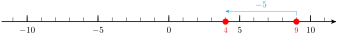
\includegraphics[width=\linewidth]{images/fig-2-1-7}
\end{sbspanel}%
\end{sidebyside}%
\end{assemblage}
\begin{assemblage}{Look Closer.}{g:assemblage:idm46056767929632}%
We see that subtracting a positive number has the same result as adding the negative number with the same absolute value. Thus, to subtract a positive number, we add its opposite.%
\end{assemblage}
\end{subsectionptx}
%
%
\typeout{************************************************}
\typeout{Subsection  Subtracting a Negative Number}
\typeout{************************************************}
%
\begin{subsectionptx}{Subtracting a Negative Number}{}{Subtracting a Negative Number}{}{}{g:subsection:idm46056767932880}
\index{number line!subtracting a negative number}%
\begin{introduction}{}%
When we add a negative number we move to the left on the number line. There are only two directions we can move on a number line, so when we subtract a negative number we must move to the right.%
\begin{assemblage}{Subtracting a negative number.}{g:assemblage:idm46056768291760}%
Compare the graphs for adding \(-3\) and subtracting \(-3\)%
\begin{itemize}[label=\textbullet]
\item{}Addition:	\(~~~~5+(-3)~~~~\)   Move 3 units to the left, to get 2.%
\begin{sidebyside}{1}{0.125}{0.125}{0}%
\begin{sbspanel}{0.75}%
\resizebox{\linewidth}{!}{%
      \tikzset{%
      }
\begin{tikzpicture} [scale=0.5]
\draw[black,thick,->,>=stealth'] (-11.8,0) -- (11.8,0);
\foreach \x in  {-11, -10,...,11} {
 \draw[black] (\x,0.3) --++(0,-0.3);
}
\foreach \x in  {-10, -5, 0,5, 10} {
 \draw[black, thick] (\x,.45) --++(0,-0.45)  node[below, yshift=-2, scale=.9]   {$\x$};
}
\foreach \x in {2} {
 \filldraw[red] (\x,0) circle (.2) node[below, yshift=-3, scale=.8] {$\x$};
}
\filldraw[red] (5,0) circle (.2);
\draw[cyan, ->, >=stealth'] (5,.53)--++(0,.3)--++(-3,0) node[above, midway, scale=.9]{$-3$};
      \end{tikzpicture}
}%
\end{sbspanel}%
\end{sidebyside}%
\item{}Subtraction:  \(~~~~5-(-3)~~~~\)   Move 3 units to the right, to get 8.%
\begin{sidebyside}{1}{0.125}{0.125}{0}%
\begin{sbspanel}{0.75}%
\resizebox{\linewidth}{!}{%
      \tikzset{%
      }
\begin{tikzpicture} [scale=0.5]
\draw[black,thick,->,>=stealth'] (-11.8,0) -- (11.8,0);
\foreach \x in  {-11, -10,...,11} {
 \draw[black] (\x,0.3) --++(0,-0.3);
}
\foreach \x in  {-10, -5, 0,5, 10} {
 \draw[black, thick] (\x,.45) --++(0,-0.45)  node[below, yshift=-2, scale=.9]   {$\x$};
}
\foreach \x in {8} {
 \filldraw[red] (\x,0) circle (.2) node[below, yshift=-3, scale=.8] {$\x$};
}
\filldraw[red] (5,0) circle (.2);
\draw[cyan, ->, >=stealth'] (5,.53)--++(0,.3)--++(3,0) node[above, midway, scale=.9]{$-(-3)$};
      \end{tikzpicture}
}%
\end{sbspanel}%
\end{sidebyside}%
\end{itemize}
%
\end{assemblage}
\begin{assemblage}{Look Closer.}{g:assemblage:idm46056773167088}%
Notice that%
\begin{equation*}
5-(-3)=8 ~~~~~ \text{and} ~~~~~5+(+3)=8
\end{equation*}
Subtracting a negative number has the same result as adding the positive number with the same absolute value. Thus, to subtract a negative number, we add its opposite.%
\end{assemblage}
\end{introduction}%
%
%
\typeout{************************************************}
\typeout{Subsubsection  Reading Questions}
\typeout{************************************************}
%
\begin{subsubsectionptx}{Reading Questions}{}{Reading Questions}{}{}{g:subsubsection:idm46056773172688}
\begin{inlineexercise}{}{g:exercise:idm46056773174752}%
True or False: \(-x\) always represents a negative number.  Give an example to support your answer.%
\par\smallskip%
\noindent\textbf{\blocktitlefont Answer}.\hypertarget{g:answer:idm46056773181536}{}\quad{}False.  If \(x=-3\), then \(-x=3\).%
\end{inlineexercise}
\begin{inlineexercise}{}{g:exercise:idm46056773190368}%
Subtracting a negative number is the same as \fillin{2.727272727272727} with the same absolute value.%
\par\smallskip%
\noindent\textbf{\blocktitlefont Answer}.\hypertarget{g:answer:idm46056773197152}{}\quad{}adding a positive number%
\end{inlineexercise}
\end{subsubsectionptx}
\end{subsectionptx}
%
%
\typeout{************************************************}
\typeout{Subsection  Subtracting Signed Numbers}
\typeout{************************************************}
%
\begin{subsectionptx}{Subtracting Signed Numbers}{}{Subtracting Signed Numbers}{}{}{g:subsection:idm46056773199216}
From the examples above, we see that to subtract any number, positive or negative, we add its opposite. We can do this in steps as follows.%
\begin{assemblage}{Rules for Subtracting Integers.}{g:assemblage:idm46056773204224}%
To subtract \(b\) from \(a\):%
\begin{enumerate}[label=\arabic*]
\item{}Change the sign of \(b\).%
\item{}Change the subtraction to addition.%
\item{}Proceed as in addition.%
\end{enumerate}
%
\end{assemblage}
This rule tells us that we can rewrite every subtraction problem as an addition problem by changing the sign of the second number.%
\begin{example}{}{g:example:idm46056769115984}%
Rewrite each subtraction problem as an addition, then compute the answer.%
\begin{multicols}{2}
\begin{enumerate}[label=\alph*]
\item{}\begin{sidebyside}{1}{0.025}{0.025}{0}%
\begin{sbspanel}{0.95}%
\resizebox{\linewidth}{!}{%
\tikzset{%
}
\begin{tikzpicture} 
\coordinate (O) at (0,0);
\node at (O) {$3 -(+10)=3+(-10)=-7$};
\coordinate(A) at (-2,0.15);
\coordinate(B) at (-2.2,.8);
\draw[blue, ->, >=stealth'] (A) to [out=100, in=180, looseness=2, edge node={node[above right, xshift=2, yshift=-3, scale=.8] {change to addition}}] (B);
\coordinate(A) at (0.49,0.8);
\coordinate(B) at (0.2,.25);
\draw[blue, ->, >=stealth'] (A) to [out=0, in=70, looseness=2] (B);
\coordinate(A) at (-1.4,-0.25);
\coordinate(B) at (-1.,-.8);
\draw[blue, ->, >=stealth'] (A) to [out=270, in=180, looseness=2, edge node={node[below right, xshift=9, yshift=4, scale=.8] {change sign}}] (B);
\coordinate(A) at (.6,-0.8);
\coordinate(B) at (.8,-.25);
\draw[blue, ->, >=stealth'] (A) to [out=0, in=270, looseness=2] (B);
\end{tikzpicture}
}%
\end{sbspanel}%
\end{sidebyside}%
%
\item{}\begin{sidebyside}{1}{0.025}{0.025}{0}%
\begin{sbspanel}{0.95}%
\resizebox{\linewidth}{!}{%
\tikzset{%
}
\begin{tikzpicture} 
\coordinate (O) at (0,0);
\node at (O) {$-6-(+3)=-6+(-3)=-9$};
\coordinate(A) at (-1.8,0.15);
\coordinate(B) at (-1.95,.8);
\draw[blue, ->, >=stealth'] (A) to [out=100, in=180, looseness=2, edge node={node[above right, xshift=2, yshift=-3, scale=.8] {change to addition}}] (B);
\coordinate(A) at (0.69,0.8);
\coordinate(B) at (0.5,.25);
\draw[blue, ->, >=stealth'] (A) to [out=0, in=70, looseness=2] (B);
\coordinate(A) at (-1.2,-0.25);
\coordinate(B) at (-0.8,-.8);
\draw[blue, ->, >=stealth'] (A) to [out=270, in=180, looseness=2, edge node={node[below right, xshift=9, yshift=4, scale=.8] {change sign}}] (B);
\coordinate(A) at (.8,-0.8);
\coordinate(B) at (1,-.25);
\draw[blue, ->, >=stealth'] (A) to [out=0, in=270, looseness=2] (B);
\end{tikzpicture}
}%
\end{sbspanel}%
\end{sidebyside}%
%
\item{}\begin{sidebyside}{1}{0.1}{0.1}{0}%
\begin{sbspanel}{0.8}%
\resizebox{\linewidth}{!}{%
\tikzset{%
}
\begin{tikzpicture} 
\coordinate (O) at (0,0);
\node at (O) {$2 -(-6)=2+(+6)=8$};
\coordinate(A) at (-1.65,0.15);
\coordinate(B) at (-1.95,.8);
\draw[blue, ->, >=stealth'] (A) to [out=100, in=180, looseness=2, edge node={node[above right, xshift=2, yshift=-3, scale=.8] {change to addition}}] (B);
\coordinate(A) at (0.69,0.8);
\coordinate(B) at (0.3,.25);
\draw[blue, ->, >=stealth'] (A) to [out=0, in=70, looseness=2] (B);
\coordinate(A) at (-1,-0.25);
\coordinate(B) at (-0.8,-.8);
\draw[blue, ->, >=stealth'] (A) to [out=270, in=180, looseness=2, edge node={node[below right, xshift=7, yshift=4, scale=.8] {change sign}}] (B);
\coordinate(A) at (.85,-0.8);
\coordinate(B) at (.9,-.25);
\draw[blue, ->, >=stealth'] (A) to [out=0, in=270, looseness=2] (B);
\end{tikzpicture}
}%
\end{sbspanel}%
\end{sidebyside}%
%
\item{}\begin{sidebyside}{1}{0.025}{0.025}{0}%
\begin{sbspanel}{0.95}%
\resizebox{\linewidth}{!}{%
\tikzset{%
}
\begin{tikzpicture} 
\coordinate (O) at (0,0);
\node at (O) {$-7-(-4)=-7+(+4)=-3$};
\coordinate(A) at (-1.8,0.15);
\coordinate(B) at (-1.95,.8);
\draw[blue, ->, >=stealth'] (A) to [out=100, in=180, looseness=2, edge node={node[above right, xshift=2, yshift=-3, scale=.8] {change to addition}}] (B);
\coordinate(A) at (0.69,0.8);
\coordinate(B) at (0.5,.25);
\draw[blue, ->, >=stealth'] (A) to [out=0, in=70, looseness=2] (B);
\coordinate(A) at (-1.2,-0.25);
\coordinate(B) at (-0.8,-.8);
\draw[blue, ->, >=stealth'] (A) to [out=270, in=180, looseness=2, edge node={node[below right, xshift=9, yshift=4, scale=.8] {change sign}}] (B);
\coordinate(A) at (.8,-0.8);
\coordinate(B) at (1,-.25);
\draw[blue, ->, >=stealth'] (A) to [out=0, in=270, looseness=2] (B);
\end{tikzpicture}
}%
\end{sbspanel}%
\end{sidebyside}%
%
\end{enumerate}
\end{multicols}
%
\end{example}
\begin{assemblage}{Look Closer.}{g:assemblage:idm46056782503888}%
At first it may be difficult to understand why subtracting a negative number is the same as adding a positive number.  Try thinking in terms of debts and assets. For example, suppose you have \textdollar{}25 in your wallet, and you have \textdollar{}5 in your hand to pay off a debt you owe a friend. If your friend now cancels (or subtracts) the debt, you are actually \textdollar{}5 richer:%
\begin{equation*}
25-(-5)=30
\end{equation*}
%
\end{assemblage}
\begin{warning}{}{g:warning:idm46056782502912}%
For simple subtractions we don't really need the subtraction rule. For example, we can subtract \(11-5\)  just as we did in arithmetic:%
\begin{equation*}
11-5=6
\end{equation*}
However, if the subtraction involves negative numbers, it is usually easier to use the subtraction rule.  Thus,%
\begin{equation*}
11-(-5)=11+(+5)=16
\end{equation*}
%
\end{warning}
\begin{assemblage}{Look Ahead.}{g:assemblage:idm46056782501264}%
We can interpret the expression \(7-9\) either as a subtraction or as an addition:%
\begin{equation*}
7-(+9) ~~~~~ \text{or} ~~~~~ 7+(-9)
\end{equation*}
Both give the same result, \(-2\).  Because addition is easier than subtraction, it is better to think of a long expression such as%
\begin{equation*}
7-9+12-6
\end{equation*}
as a sum of signed numbers. To do this, we add all the numbers together, and the \(+\) or \(-\) sign in front of each number tells us whether that number is positive or negative.%
\end{assemblage}
Remember that additions should be performed in order from left to right.%
\begin{example}{}{g:example:idm46056769149424}%
Simplify \(~~7-9+12-6\)%
\par\smallskip%
\noindent\textbf{\blocktitlefont Solution}.\hypertarget{g:solution:idm46056769153264}{}\quad{}We add the signed numbers \(7\) and \(-9\) and \(12\) and \(-6\), in order from left to right.%
\begin{align*}
\blert{7-9}+12-6 \amp =\blert{-2}+12-6 \amp \amp \blert{\text{The sum of} ~7~ \text{and}~-9~\text{is}~-2.}\\
\amp =10-6=4 \amp \amp \blert{\text{The sum of}~-2~\text{and}~12~\text{is}~10.}
\end{align*}
%
\end{example}
\begin{warning}{}{g:warning:idm46056769173280}%
The following calculation is incorrect:%
\begin{equation*}
16-\blert{9-4}+3~=~16-\blert{5}+3~=~11+3~=~14~~~~~~\alert {\leftarrow \text{Incorrect!}}
\end{equation*}
We must perform additions and subtractions in order from left to right:%
\begin{equation*}
\blert{16-9}-4+3~=~\blert{7}-4+3~=~3+3~=~6
\end{equation*}
%
\end{warning}
\end{subsectionptx}
%
%
\typeout{************************************************}
\typeout{Subsection  Multiplying Signed Numbers}
\typeout{************************************************}
%
\begin{subsectionptx}{Multiplying Signed Numbers}{}{Multiplying Signed Numbers}{}{}{g:subsection:idm46056769291488}
\index{signed number!multiplying}%
\index{multiplication!of signed numbers}%
\index{product!of signed numbers}%
%
%
\typeout{************************************************}
\typeout{Subsubsection  Case 1: The product of numbers with opposite signs}
\typeout{************************************************}
%
\begin{subsubsectionptx}{Case 1: The product of numbers with opposite signs}{}{Case 1: The product of numbers with opposite signs}{}{}{g:subsubsection:idm46056769354576}
We can think of multiplication as repeated addition.  For example,%
\begin{equation*}
3(2)~~~~~\text{means}~~~~~2+2+2~~~~~\text{The sum of three 2's}
\end{equation*}
Similarly,%
\begin{equation*}
3(-2)~~~~~\text{means}~~~~~-2+(-2)+(-2)~~~~~\text{The sum of three}~ -2\text{'s}
\end{equation*}
which is \(-6\), so \(3(-2)=-6\).  Think in terms of money:  if you owe three different people 2 dollars each, then you are 6 dollars in debt.%
\par
Because multiplication is commutative, it is also true that \(-2(3)=-6\). This example illustrates the following fact.%
\begin{assemblage}{Products.}{g:assemblage:idm46056769384576}%
The product of a positive number and a negative number is a negative number.%
\end{assemblage}
\begin{example}{}{g:example:idm46056769726992}%
You can use your calculator to verify the following products.%
\begin{multicols}{2}
\begin{enumerate}[label=\alph*]
\item{}\(\displaystyle (-4)(7)=-28\)%
\item{}\(\displaystyle 5(-2.6)=-13\)%
\end{enumerate}
\end{multicols}
%
\end{example}
\end{subsubsectionptx}
%
%
\typeout{************************************************}
\typeout{Subsubsection  Case 2: The product of numbers with the same sign}
\typeout{************************************************}
%
\begin{subsubsectionptx}{Case 2: The product of numbers with the same sign}{}{Case 2: The product of numbers with the same sign}{}{}{g:subsubsection:idm46056769827376}
You know that the product of two positive numbers is positive. It is also true that the product of two negative numbers is positive.%
\par
To understand why the product of two negative numbers is positive, you might think of canceling, or subtracting, several debts of the same amount. Or, you could observe the pattern in the lists of products below.  As we move down the list, the product increases by equal amounts.%
\begin{align*}
3(-2) \amp =-6 \amp  3(-5) \amp =-15\\
2(-2) \amp =-4 \amp  2(-5) \amp =-10\\
1(-2) \amp =-2 \amp  1(-5) \amp =-5~~\amp \blert{\leftarrow \text{Positive times negative is negative.}}\\
0(-2) \amp =-0 \amp  0(-5) \amp =0\\
-1(-2) \amp =2 \amp  -1(-5) \amp =5~~\amp \blert{\leftarrow \text{Negative times negative is positive.}}\\
-2(-2) \amp =4 \amp  -2(-5) \amp =10\\
-3(-2) \amp =6 \amp  -3(-5) \amp =15
\end{align*}
Based on the pattern in these calculations, the following rule seems reasonable.%
\begin{assemblage}{More Products.}{g:assemblage:idm46056769870144}%
The product of two negative numbers is a positive number.%
\end{assemblage}
\begin{example}{}{g:example:idm46056769873680}%
You can use your calculator to verify the following products.%
\begin{multicols}{2}
\begin{enumerate}[label=\alph*]
\item{}\(\displaystyle (-6)(-3)=18\)%
\item{}\(\displaystyle (-2.1)(-3.4)=7.14\)%
\end{enumerate}
\end{multicols}
%
\end{example}
Now we have a pair of rules about the products of signed numbers.%
\begin{assemblage}{Products of Signed Numbers.}{g:assemblage:idm46056769905872}%
%
\begin{enumerate}[label=\arabic*]
\item{}The product of two numbers with opposite signs is a negative number.%
\item{}The product of two numbers with the same sign is a positive number.%
\end{enumerate}
%
\end{assemblage}
\end{subsubsectionptx}
\end{subsectionptx}
%
%
\typeout{************************************************}
\typeout{Subsection  Dividing Signed Numbers}
\typeout{************************************************}
%
\begin{subsectionptx}{Dividing Signed Numbers}{}{Dividing Signed Numbers}{}{}{g:subsection:idm46056769938912}
\index{signed number!division of}%
\index{division!of signed numbers}%
\index{quotient!of signed numbers}%
\begin{introduction}{}%
Division is the inverse operation for multiplication. For example, we know that%
\begin{equation*}
\dfrac{12}{3}=\alert{4}~~~~~~\text{because}~~~~~~3 \cdot \alert{4} = 12
\end{equation*}
Thus, every division fact can be converted into an equivalent multiplication fact. For example,%
\begin{equation*}
\text{The division fact}~~\dfrac{\blert{400}}{16}=25~~~~\text{is equivalent to}~~~~16 \cdot 25 = \blert{400}
\end{equation*}
Note that the numerator in the division fact becomes the product in the multiplication fact. The same relationship between multiplication and division holds for negative numbers as well.%
\begin{example}{}{g:example:idm46056769978000}%
Rewrite each division fact as a multiplication fact.%
\begin{multicols}{2}
\begin{enumerate}[label=\alph*]
\item{}\(\displaystyle \dfrac{-144}{64}=-2.25\)%
\item{}\(\displaystyle -36 \div \dfrac{-3}{8}=96\)%
\end{enumerate}
\end{multicols}
%
\par\smallskip%
\noindent\textbf{\blocktitlefont Solution}.\hypertarget{g:solution:idm46056769987760}{}\quad{}The numerator in each division fact becomes the product in the multiplication fact.%
\begin{multicols}{2}
\begin{enumerate}[label=\alph*]
\item{}\(\displaystyle -144=-2.25(64)\)%
\item{}\(\displaystyle -36= \dfrac{-3}{8}(96)\)%
\end{enumerate}
\end{multicols}
%
\end{example}
The Example above illustrates the rules for division of signed numbers.%
\begin{assemblage}{Quotients of Signed Numbers.}{g:assemblage:idm46056770078496}%
%
\begin{enumerate}[label=\alph*]
\item{}The quotient of two numbers with opposite signs is a negative number.%
\item{}The quotient of two numbers with the same sign is a positive number.%
\end{enumerate}
%
\end{assemblage}
\end{introduction}%
%
%
\typeout{************************************************}
\typeout{Subsubsection  Reading Questions}
\typeout{************************************************}
%
\begin{subsubsectionptx}{Reading Questions}{}{Reading Questions}{}{}{g:subsubsection:idm46056770325232}
\begin{inlineexercise}{}{g:exercise:idm46056770328176}%
Which of these is a product?%
\begin{multicols}{4}
\begin{enumerate}[label=\alph*]
\item{}\(\displaystyle 3+(-4)\)%
\item{}\(\displaystyle -3-4\)%
\item{}\(\displaystyle -3(-4)\)%
\item{}\(\displaystyle 3-(-4)\)%
\end{enumerate}
\end{multicols}
%
\par\smallskip%
\noindent\textbf{\blocktitlefont Answer}.\hypertarget{g:answer:idm46056770392320}{}\quad{}c%
\end{inlineexercise}
\begin{inlineexercise}{}{g:exercise:idm46056770394384}%
Rewrite the division fact \(\dfrac{48}{D}=Q\) as a multiplication fact.%
\par\smallskip%
\noindent\textbf{\blocktitlefont Answer}.\hypertarget{g:answer:idm46056770401744}{}\quad{}\(DQ=48\)%
\end{inlineexercise}
Remember that a fraction can be thought of as a division. For example, \(\dfrac{3}{4}\) means \(3 \div 4\), or 0.75. What about negative fractions?%
\begin{itemize}[label=\textbullet]
\item{}Because the quotient of two numbers with unlike signs is negative, the fractions \(\dfrac{-3}{4}\) and \(\dfrac{3}{-4}\) both represent the negative number \(-\dfrac{3}{4}\).%
\item{}On the other hand, \(\dfrac{-3}{-4}\) is equal to the positive number \(\dfrac{3}{4}\).%
\end{itemize}
%
\par
For many of the calculations in algebra, it is more convenient to write a negative fraction with the minus sign in the numerator, like this: \(\dfrac{-3}{4}\).%
\begin{assemblage}{Standard Form for Fractions.}{g:assemblage:idm46056770497456}%
A negative fraction is written in \terminology{standard form} when the minus sign is in the numerator:  \(\dfrac{-a}{b}\).%
\begin{equation*}
\blert{\dfrac{-a}{b}}=\dfrac{a}{-b}=-\dfrac{a}{b}
\end{equation*}
The standard form for a positive fraction has positive numerator and denominator.%
\begin{equation*}
\blert{\dfrac{a}{b}}=\dfrac{-a}{-b}
\end{equation*}
%
\end{assemblage}
\end{subsubsectionptx}
\end{subsectionptx}
%
%
\typeout{************************************************}
\typeout{Subsection  Quotients Involving Zero}
\typeout{************************************************}
%
\begin{subsectionptx}{Quotients Involving Zero}{}{Quotients Involving Zero}{}{}{g:subsection:idm46056770520864}
\index{quotient!involving zero}%
\index{division!involving zero}%
\begin{introduction}{}%
What is the meaning of an expression such as \(\dfrac{0}{2}\)? We can rewrite this quotient as an equivalent multiplication fact.%
\begin{equation*}
\dfrac{0}{2}=\alert{?}~~~~\text{is equivalent to}~~~~2 \cdot \alert{?} = 0
\end{equation*}
What number can we substitute for the question mark to make \(~2 \cdot \alert{?} = 0~\) a true statement? The only solution for this equation is \(0\). Thus, replacing the question marks by \(0\) we have%
\begin{equation*}
\dfrac{0}{2}=\alert{0}~~~~\text{because}~~~~2 \cdot \alert{0} = 0
\end{equation*}
In general, 0 divided by any (non-zero) number is 0.%
\par
Now consider a quotient with zero in the denominator, such as \(\dfrac{2}{0}\).%
\begin{equation*}
\dfrac{2}{0}=\alert{?}~~~~\text{is equivalent to}~~~~0 \cdot \alert{?} = 2
\end{equation*}
What number can we substitute for the question mark to make \(~0 \cdot \alert{?} = 2~\) a true statement? This equation has no solution, because 0 times any number is 0, not 2.  Thus, there is no answer for the division problem \(\dfrac{2}{0}\). We say that the quotient \(\dfrac{2}{0}\) is \terminology{undefined}\index{undefined!quotient}. In general, we cannot divide any number by zero.\index{undefined!division by zero}%
\begin{assemblage}{Quotients Involving Zero.}{g:assemblage:idm46056770610784}%
If \(a\) is any nonzero number, then%
\begin{equation*}
\blert{\dfrac{0}{a} = 0}~~~~~~\text{and}~~~~~~ \blert{\dfrac{a}{0} ~~ \text{is undefined.}}
\end{equation*}
%
\end{assemblage}
\begin{example}{}{g:example:idm46056783798352}%
%
\begin{multicols}{2}
\begin{enumerate}[label=\alph*]
\item{}\(6 \div 0~~\) is undefined.%
\item{}\(\displaystyle 0 \div 8=0\)%
\end{enumerate}
\end{multicols}
%
\end{example}
\end{introduction}%
%
%
\typeout{************************************************}
\typeout{Subsubsection  Reading Questions}
\typeout{************************************************}
%
\begin{subsubsectionptx}{Reading Questions}{}{Reading Questions}{}{}{g:subsubsection:idm46056771665632}
\begin{inlineexercise}{}{g:exercise:idm46056771667696}%
Which of these is undefined?  \(~\dfrac{-6}{0}~\) or \(~\dfrac{0}{-6}~\)?%
\par\smallskip%
\noindent\textbf{\blocktitlefont Answer}.\hypertarget{g:answer:idm46056772333264}{}\quad{}\(\dfrac{-6}{0}\)%
\end{inlineexercise}
\end{subsubsectionptx}
\end{subsectionptx}
%
%
\typeout{************************************************}
\typeout{Subsection  Skills Warm-Up}
\typeout{************************************************}
%
\begin{subsectionptx}{Skills Warm-Up}{}{Skills Warm-Up}{}{}{g:subsection:idm46056772335920}
\begin{assemblage}{Good work!}{g:assemblage:idm46056772337696}%
You've finished the Reading assignment for Section 2.1.  Now try the Skills Warm-Up Exercises before the next class meeting.%
\end{assemblage}
%
%
\typeout{************************************************}
\typeout{Exercises  Exercises}
\typeout{************************************************}
%
\begin{exercises-subsubsection}{Exercises}{}{Exercises}{}{}{g:exercises:idm46056772341536}
\begin{divisionexercise}{1}{}{}{g:exercise:idm46056772342128}%
Graph the numbers on the number line:  \(0,~-3,~3,~\dfrac{1}{2},~\dfrac{-5}{3},~5\dfrac{1}{4}\)%
\begin{sidebyside}{1}{0.15}{0.15}{0}%
\begin{sbspanel}{0.7}%
\resizebox{\linewidth}{!}{%
\tikzset{%
}
\begin{tikzpicture} [scale=0.45]
\draw[black,thick,->,>=stealth'] (-11.8,0) -- (11.8,0);
\foreach \x in  {-11, -10,...,11} {
 \draw[black] (\x,0.3) --++(0,-0.3);
}
\foreach \x in  {-10, -5, ..., 10} {
 \draw[black, thick] (\x,.45) --++(0,-0.45)  node[below]   {$\x$};
}
\end{tikzpicture}
}%
\end{sbspanel}%
\end{sidebyside}%
\end{divisionexercise}%
\begin{divisionexercise}{2}{}{}{g:exercise:idm46056772360256}%
Graph the numbers on the number line:  \(-4.5,~-2,~-1.4,~0.6,~2\)%
\begin{sidebyside}{1}{0.15}{0.15}{0}%
\begin{sbspanel}{0.7}%
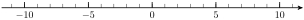
\includegraphics[width=\linewidth]{images/sw-2-1-1}
\end{sbspanel}%
\end{sidebyside}%
\end{divisionexercise}%
\par\medskip\noindent%
%
Replace the comma in each pair by the proper symbol, \(\lt,~\gt,~\) or \(=\).%
\begin{exercisegroup}
\begin{divisionexerciseeg}{3}{}{}{g:exercise:idm46056772378544}%
%
\begin{multicols}{2}
\begin{enumerate}[label=\alph*]
\item{}\(\displaystyle 0,~-4\)%
\item{}\(\displaystyle -5,~-9\)%
\item{}\(\displaystyle -2\frac{5}{8}~,-2\frac{1}{8}\)%
\item{}\(\displaystyle 13.6,~13.66\)%
\end{enumerate}
\end{multicols}
%
\end{divisionexerciseeg}%
\begin{divisionexerciseeg}{4}{}{}{g:exercise:idm46056772396128}%
%
\begin{multicols}{2}
\begin{enumerate}[label=\alph*]
\item{}\(\displaystyle 3,~-7\)%
\item{}\(\displaystyle -1,~-6\)%
\item{}\(\displaystyle -3~,-3\frac{3}{4}\)%
\item{}\(\displaystyle -18.4,~-19.6\)%
\end{enumerate}
\end{multicols}
%
\end{divisionexerciseeg}%
\end{exercisegroup}
\par\medskip\noindent
\end{exercises-subsubsection}
%
%
\typeout{************************************************}
\typeout{Solutions  Answers to Skills Warm-Up}
\typeout{************************************************}
%
\begin{solutions-subsubsection}{Answers to Skills Warm-Up}{}{Answers to Skills Warm-Up}{}{}{g:solutions:idm46056772415712}
\begin{conclusion}{}%
%
\begin{enumerate}[label=\arabic*]
\item{}\begin{sidebyside}{1}{0.15}{0.15}{0}%
\begin{sbspanel}{0.7}%
\resizebox{\linewidth}{!}{%
\tikzset{%
}
\begin{tikzpicture} [scale=0.45]
\draw[black,thick,->,>=stealth'] (-11.8,0) -- (11.8,0);
\foreach \x in  {-11, -10,...,11} {
 \draw[black] (\x,0.3) --++(0,-0.3);
}
\foreach \x in  {-10, -5, ..., 10} {
 \draw[black, thick] (\x,.45) --++(0,-0.45)  node[below]   {$\x$};
}
\foreach \x in {-3,3} {
 \filldraw[red] (\x,0) circle (.15) node[above, yshift=3, scale=.9] {$\x$};
}
\filldraw[red] (1/2,0) circle (.15) node[above, yshift=3, scale=.9] {$\frac{1}{2}$}; 
\filldraw[red] (-5/3,0) circle (.15) node[above, yshift=3, scale=.9] {$\frac{-5}{3}$}; 
 \filldraw[red] (0,0) circle (.15);
\filldraw[red] (21/4,0) circle (.15) node[above, yshift=3, scale=.9] {$5\frac{1}{4}$};
\end{tikzpicture}
}%
\end{sbspanel}%
\end{sidebyside}%
%
\item{}\begin{sidebyside}{1}{0.15}{0.15}{0}%
\begin{sbspanel}{0.7}%
\resizebox{\linewidth}{!}{%
\tikzset{%
}
\begin{tikzpicture} [scale=0.45]
\draw[black,thick,->,>=stealth'] (-11.8,0) -- (11.8,0);
\foreach \x in  {-11, -10,...,11} {
 \draw[black] (\x,0.3) --++(0,-0.3);
}
\foreach \x in  {-10, -5, ..., 10} {
 \draw[black, thick] (\x,.45) --++(0,-0.45)  node[below]   {$\x$};
}
\foreach \x in {-4.5,-1.4, 0.6, 2} {
 \filldraw[red] (\x,0) circle (.15) node[above, yshift=3, scale=.9] {$\x$};
}
\filldraw[red] (-2,0) circle (.15) node[below, yshift=-3, scale=.9] {$-2$};
\end{tikzpicture}
}%
\end{sbspanel}%
\end{sidebyside}%
%
\item{}%
\begin{multicols}{4}
\begin{enumerate}[label=\alph*]
\item{}\(\displaystyle \gt\)%
\item{}\(\displaystyle \gt\)%
\item{}\(\displaystyle \lt\)%
\item{}\(\displaystyle \lt\)%
\end{enumerate}
\end{multicols}
%
\item{}%
\begin{multicols}{4}
\begin{enumerate}[label=\alph*]
\item{}\(\displaystyle \gt\)%
\item{}\(\displaystyle \gt\)%
\item{}\(\displaystyle \gt\)%
\item{}\(\displaystyle \gt\)%
\end{enumerate}
\end{multicols}
%
\end{enumerate}
%
\end{conclusion}%
\end{solutions-subsubsection}
\end{subsectionptx}
%
%
\typeout{************************************************}
\typeout{Subsection  Lesson}
\typeout{************************************************}
%
\begin{subsectionptx}{Lesson}{}{Lesson}{}{}{g:subsection:idm46056784669648}
\begin{introduction}{}%
\begin{activity}{Sums and Differences.}{g:activity:idm46056784669136}%
%
\begin{enumerate}[label=\arabic*]
\item{}Illustrate each sum on a number line, then give the answer.%
\begin{enumerate}[label=\alph*]
\item{}\(\displaystyle 2+4=\)%
\begin{sidebyside}{1}{0.15}{0.15}{0}%
\begin{sbspanel}{0.7}%
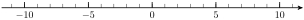
\includegraphics[width=\linewidth]{images/sw-2-1-1}
\end{sbspanel}%
\end{sidebyside}%
\item{}\(\displaystyle (-4)+(-7)=\)%
\begin{sidebyside}{1}{0.15}{0.15}{0}%
\begin{sbspanel}{0.7}%
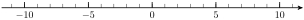
\includegraphics[width=\linewidth]{images/sw-2-1-1}
\end{sbspanel}%
\end{sidebyside}%
\item{}\(\displaystyle (-6)+(-3)=\)%
\begin{sidebyside}{1}{0.15}{0.15}{0}%
\begin{sbspanel}{0.7}%
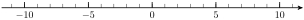
\includegraphics[width=\linewidth]{images/sw-2-1-1}
\end{sbspanel}%
\end{sidebyside}%
\end{enumerate}
%
\item{}Illustrate each sum on a number line, then give the answer.%
\begin{enumerate}[label=\alph*]
\item{}\(\displaystyle (+5)+(-3)=\)%
\begin{sidebyside}{1}{0.15}{0.15}{0}%
\begin{sbspanel}{0.7}%
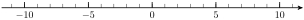
\includegraphics[width=\linewidth]{images/sw-2-1-1}
\end{sbspanel}%
\end{sidebyside}%
\item{}\(\displaystyle (-7)+(+2)=\)%
\begin{sidebyside}{1}{0.15}{0.15}{0}%
\begin{sbspanel}{0.7}%
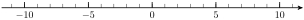
\includegraphics[width=\linewidth]{images/sw-2-1-1}
\end{sbspanel}%
\end{sidebyside}%
\item{}\(\displaystyle (-5)+(+9)=\)%
\begin{sidebyside}{1}{0.15}{0.15}{0}%
\begin{sbspanel}{0.7}%
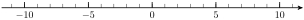
\includegraphics[width=\linewidth]{images/sw-2-1-1}
\end{sbspanel}%
\end{sidebyside}%
\end{enumerate}
%
\item{}Fill in the blanks.%
\begin{enumerate}[label=\alph*]
\item{}The sum of two positive numbers is \fillin{5.454545454545454}.%
\item{}The sum of two negative numbers is \fillin{5.454545454545454}.%
\item{}To add two numbers with opposite signs, \fillin{5.454545454545454} their absolute values. The sum has the same sign as the number with the \fillin{5.454545454545454} absolute value.%
\end{enumerate}
%
\item{}Find the following sums.%
\begin{multicols}{2}
\begin{enumerate}[label=\alph*]
\item{}\(\displaystyle (-9)+(-9)\)%
\item{}\(\displaystyle (-14)+(-11)\)%
\item{}\(\displaystyle 4+(-12)\)%
\item{}\(\displaystyle 15+(-9)\)%
\item{}\(\displaystyle -6+(-3)\)%
\item{}\(\displaystyle -8+(+3)\)%
\item{}\(\displaystyle -7+19\)%
\item{}\(\displaystyle 18+(-10)\)%
\item{}\(\displaystyle 5+(-5)\)%
\item{}\(\displaystyle -5+(-5)\)%
\end{enumerate}
\end{multicols}
%
\item{}Illustrate each sum on a number line, then give the answer.%
\begin{enumerate}[label=\alph*]
\item{}\(\displaystyle 2-(-6)=\)%
\begin{sidebyside}{1}{0.15}{0.15}{0}%
\begin{sbspanel}{0.7}%
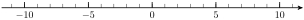
\includegraphics[width=\linewidth]{images/sw-2-1-1}
\end{sbspanel}%
\end{sidebyside}%
\item{}\(\displaystyle -7-(-4)=\)%
\begin{sidebyside}{1}{0.15}{0.15}{0}%
\begin{sbspanel}{0.7}%
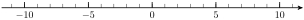
\includegraphics[width=\linewidth]{images/sw-2-1-1}
\end{sbspanel}%
\end{sidebyside}%
\item{}\(\displaystyle -3-(-7)=\)%
\begin{sidebyside}{1}{0.15}{0.15}{0}%
\begin{sbspanel}{0.7}%
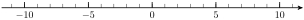
\includegraphics[width=\linewidth]{images/sw-2-1-1}
\end{sbspanel}%
\end{sidebyside}%
\end{enumerate}
%
\item{}Rewrite each subtraction problem as an addition, then compute the answer.%
\begin{enumerate}[label=\alph*]
\item{}\(\displaystyle 3-(-9)=\)%
\item{}\(\displaystyle -4-(-7)=\)%
\item{}\(\displaystyle -8-(-2)=\)%
\end{enumerate}
%
\end{enumerate}
%
\end{activity}
\begin{activity}{Products and Quotients.}{g:activity:idm46056773973296}%
%
\begin{enumerate}[label=\arabic*]
\item{}Write the product \(5(-4)\) as a repeated addition, and compute the product.%
\item{}Compute the products.%
\begin{multicols}{2}
\begin{enumerate}[label=\alph*]
\item{}\(\displaystyle 5(-4)\)%
\item{}\(\displaystyle \dfrac{-3}{4} \cdot \dfrac{1}{2}\)%
\item{}\(\displaystyle (-3)(-3)\)%
\item{}\(\displaystyle \dfrac{-5}{3} \cdot \dfrac{-3}{10}\)%
\end{enumerate}
\end{multicols}
%
\item{}Use the relationship between products and quotients to complete each statement. No calculation is necessary!%
\begin{enumerate}[label=\alph*]
\item{}\(\dfrac{8190}{26} = \fillin{2.727272727272727}~~\) because \(~~26 \cdot 315 = 8190\)%
\item{}\(62 \cdot \fillin{2.727272727272727}=83.7~~\) because \(~~\dfrac{83.7}{62} = 1.35\)%
\end{enumerate}
%
\item{}Find each quotient by rewriting the division as an equivalent multiplication fact.%
\begin{multicols}{2}
\begin{enumerate}[label=\alph*]
\item{}\(\dfrac{6}{3} = \boxed{\hphantom{00}\vphantom{0000}}~~\) because \fillin{3.636363636363636}%
\item{}\(\dfrac{6}{-3} = \boxed{\hphantom{00}\vphantom{0000}}~~\) because \fillin{3.636363636363636}%
\item{}\(\dfrac{-6}{3} = \boxed{\hphantom{00}\vphantom{0000}}~~\) because \fillin{3.636363636363636}%
\item{}\(\dfrac{-6}{-3} = \boxed{\hphantom{00}\vphantom{0000}}~~\) because \fillin{3.636363636363636}%
\end{enumerate}
\end{multicols}
%
\item{}Compute the quotients.%
\begin{multicols}{2}
\begin{enumerate}[label=\alph*]
\item{}\(\displaystyle \dfrac{-25}{-5}\)%
\item{}\(\displaystyle \dfrac{32}{-8}\)%
\item{}\(\displaystyle -27 \div 9\)%
\item{}\(\displaystyle -42 \div (-7)\)%
\end{enumerate}
\end{multicols}
%
\item{}Fill in the blanks.%
\begin{enumerate}[label=\alph*]
\item{}The product or quotient of two numbers with the same sign is \fillin{3.636363636363636}.%
\item{}The product or quotient of two numbers with opposite signs is \fillin{3.636363636363636}.%
\end{enumerate}
%
\item{}Find the quotient if it exists.%
\begin{multicols}{2}
\begin{enumerate}[label=\alph*]
\item{}\(\displaystyle \dfrac{0}{18}\)%
\item{}\(\displaystyle \dfrac{13}{0}\)%
\item{}\(\displaystyle -9 \div 0\)%
\item{}\(\displaystyle 0 \div (-2)\)%
\end{enumerate}
\end{multicols}
%
\item{}%
\begin{enumerate}[label=\alph*]
\item{}Use your calculator to verify that  \(-\dfrac{2}{5} = \dfrac{-2}{5} = \dfrac{2}{-5}\)%
\item{}Does \(-\dfrac{2}{5} = \dfrac{-2}{-5}\) ?%
\end{enumerate}
%
\end{enumerate}
%
\end{activity}
\end{introduction}%
%
%
\typeout{************************************************}
\typeout{Subsubsection  Wrap-Up}
\typeout{************************************************}
%
\begin{subsubsectionptx}{Wrap-Up}{}{Wrap-Up}{}{}{g:subsubsection:idm46056774423664}
\begin{objectives}{Objectives}{g:objectives:idm46056774425312}
In this Lesson we practiced the following skills:%
%
\begin{itemize}[label=\textbullet]
\item{}Illustrating sums and differences on a number line%
\item{}Performing operations on signed numbers%
\item{}Writing a subtraction as an equivalent addition%
\end{itemize}
\end{objectives}
Questions to answer before the Homework Preview.%
\begin{outcomes}{Questions}{g:outcomes:idm46056777126400}
%
\begin{enumerate}[label=\arabic*]
\item{}Delbert says that "two negatives make a positive." For which operations is he correct, and for which is he incorrect?%
\item{}How do we convert a subtraction of signed numbers into an addition? Give an example.%
\item{}True or false:%
\begin{multicols}{2}
\begin{enumerate}[label=\alph*]
\item{}\(\displaystyle \dfrac{2}{-2} = 0\)%
\item{}\(\displaystyle \dfrac{2}{0} = 0\)%
\item{}\(\displaystyle -2-2 = 0\)%
\item{}\(\displaystyle -2(-2) = 0\)%
\end{enumerate}
\end{multicols}
%
\item{}Does the negative sign in a fraction such as \(~-\dfrac{5}{2}~\) apply to the numerator, the denominator, or both?%
\end{enumerate}
\end{outcomes}
\end{subsubsectionptx}
\end{subsectionptx}
%
%
\typeout{************************************************}
\typeout{Subsection  Homework Preview}
\typeout{************************************************}
%
\begin{subsectionptx}{Homework Preview}{}{Homework Preview}{}{}{g:subsection:idm46056777162592}
Here are exercises to try before the end of the class meeting.%
%
%
\typeout{************************************************}
\typeout{Exercises  Exercises}
\typeout{************************************************}
%
\begin{exercises-subsubsection}{Exercises}{}{Exercises}{}{}{g:exercises:idm46056777166128}
\par\medskip\noindent%
%
Perform the operations.%
\begin{exercisegroup}
\begin{divisionexerciseeg}{1}{}{}{g:exercise:idm46056777170256}%
%
\begin{multicols}{2}
\begin{enumerate}[label=\alph*]
\item{}\(\displaystyle 8+(-4)\)%
\item{}\(\displaystyle 8-(-4)\)%
\item{}\(\displaystyle -8-4\)%
\item{}\(\displaystyle -8-(-4)\)%
\end{enumerate}
\end{multicols}
%
\end{divisionexerciseeg}%
\begin{divisionexerciseeg}{2}{}{}{g:exercise:idm46056777193968}%
%
\begin{multicols}{2}
\begin{enumerate}[label=\alph*]
\item{}\(\displaystyle 8(-4)\)%
\item{}\(\displaystyle -8(-4)\)%
\item{}\(\displaystyle \dfrac{-8}{-4}\)%
\item{}\(\displaystyle \dfrac{8}{-4}\)%
\end{enumerate}
\end{multicols}
%
\end{divisionexerciseeg}%
\end{exercisegroup}
\par\medskip\noindent
\par\medskip\noindent%
%
Solve.%
\begin{exercisegroupcol}{2}
\begin{divisionexerciseegcol}{3}{}{}{g:exercise:idm46056777215072}%
\(7+x=-8\)%
\end{divisionexerciseegcol}%
\begin{divisionexerciseegcol}{4}{}{}{g:exercise:idm46056777218896}%
\(-2x=12\)%
\end{divisionexerciseegcol}%
\end{exercisegroupcol}
\par\medskip\noindent
\end{exercises-subsubsection}
%
%
\typeout{************************************************}
\typeout{Solutions  Answers to Homework Preview}
\typeout{************************************************}
%
\begin{solutions-subsubsection}{Answers to Homework Preview}{}{Answers to Homework Preview}{}{}{g:solutions:idm46056777222304}
\begin{conclusion}{}%
%
\begin{enumerate}[label=\arabic*]
\item{}%
\begin{multicols}{4}
\begin{enumerate}[label=\alph*]
\item{}\(\displaystyle 4\)%
\item{}\(\displaystyle 12\)%
\item{}\(\displaystyle -12\)%
\item{}\(\displaystyle -4\)%
\end{enumerate}
\end{multicols}
%
\item{}%
\begin{multicols}{4}
\begin{enumerate}[label=\alph*]
\item{}\(\displaystyle -32\)%
\item{}\(\displaystyle 32\)%
\item{}\(\displaystyle 2\)%
\item{}\(\displaystyle -2\)%
\end{enumerate}
\end{multicols}
%
\item{}\(\displaystyle -15\)%
\item{}\(\displaystyle -6\)%
\end{enumerate}
%
\end{conclusion}%
\end{solutions-subsubsection}
\end{subsectionptx}
%
%
\typeout{************************************************}
\typeout{Exercises  Homework 2.1}
\typeout{************************************************}
%
\begin{exercises-subsection}{Homework 2.1}{}{Homework 2.1}{}{}{g:exercises:idm46056774815648}
\par\medskip\noindent%
%
For Problems 1\textendash{}4, add.%
\begin{exercisegroup}
\begin{divisionexerciseeg}{1}{}{}{g:exercise:idm46056774823776}%
%
\begin{multicols}{3}
\begin{enumerate}[label=\alph*]
\item{}\(\displaystyle 5+(-3)\)%
\item{}\(\displaystyle -5+3\)%
\item{}\(\displaystyle -5+(-3)\)%
\end{enumerate}
\end{multicols}
%
\end{divisionexerciseeg}%
\begin{divisionexerciseeg}{2}{}{}{g:exercise:idm46056775474528}%
%
\begin{multicols}{3}
\begin{enumerate}[label=\alph*]
\item{}\(\displaystyle -15+(-20)\)%
\item{}\(\displaystyle 15+(-20)\)%
\item{}\(\displaystyle -15+20\)%
\end{enumerate}
\end{multicols}
%
\end{divisionexerciseeg}%
\begin{divisionexerciseeg}{3}{}{}{g:exercise:idm46056775505392}%
%
\begin{multicols}{3}
\begin{enumerate}[label=\alph*]
\item{}\(\displaystyle -47+22\)%
\item{}\(\displaystyle 6.8+(-2.7)\)%
\item{}\(\displaystyle -\dfrac{5}{6}+\dfrac{2}{3}\)%
\end{enumerate}
\end{multicols}
%
\end{divisionexerciseeg}%
\begin{divisionexerciseeg}{4}{}{}{g:exercise:idm46056775548112}%
%
\begin{multicols}{3}
\begin{enumerate}[label=\alph*]
\item{}\(\displaystyle -13+(-36)\)%
\item{}\(\displaystyle -2.5+4.9\)%
\item{}\(\displaystyle -\dfrac{3}{4}+(-\dfrac{3}{8})\)%
\end{enumerate}
\end{multicols}
%
\end{divisionexerciseeg}%
\end{exercisegroup}
\par\medskip\noindent
\begin{divisionexercise}{5}{}{}{g:exercise:idm46056775562256}%
Rewrite each subtraction problem as an addition problem, and give the answer.%
\begin{multicols}{2}
\begin{enumerate}[label=\alph*]
\item{}\(\displaystyle 4-8\)%
\item{}\(\displaystyle 3-(-9)\)%
\item{}\(\displaystyle -8-(-6)\)%
\item{}\(\displaystyle -6-5\)%
\end{enumerate}
\end{multicols}
%
\end{divisionexercise}%
\par\medskip\noindent%
%
For Problems 6\textendash{}8, add or subtract as indicated.%
\begin{exercisegroup}
\begin{divisionexerciseeg}{6}{}{}{g:exercise:idm46056775607136}%
%
\begin{multicols}{2}
\begin{enumerate}[label=\alph*]
\item{}\(\displaystyle 12+(-6)\)%
\item{}\(\displaystyle 6-(-4)\)%
\item{}\(\displaystyle -2-8\)%
\item{}\(\displaystyle -7+9\)%
\end{enumerate}
\end{multicols}
%
\end{divisionexerciseeg}%
\begin{divisionexerciseeg}{7}{}{}{g:exercise:idm46056775638064}%
%
\begin{multicols}{2}
\begin{enumerate}[label=\alph*]
\item{}\(\displaystyle -14-(-3)\)%
\item{}\(\displaystyle -5+(-4)\)%
\item{}\(\displaystyle -6-(-6)\)%
\item{}\(\displaystyle -4-4\)%
\end{enumerate}
\end{multicols}
%
\end{divisionexerciseeg}%
\begin{divisionexerciseeg}{8}{}{}{g:exercise:idm46056775782912}%
%
\begin{multicols}{2}
\begin{enumerate}[label=\alph*]
\item{}\(\displaystyle 24-(-10)\)%
\item{}\(\displaystyle 18+(-12)\)%
\item{}\(\displaystyle -16+14\)%
\item{}\(\displaystyle -25-(-15)\)%
\end{enumerate}
\end{multicols}
%
\end{divisionexerciseeg}%
\end{exercisegroup}
\par\medskip\noindent
\par\medskip\noindent%
%
For Problems 9\textendash{}10, compute each sum or difference in parts (a) and (b), and decide which is easier. Then decide how to simplify the expression in part (c).%
\begin{exercisegroup}
\begin{divisionexerciseeg}{9}{}{}{g:exercise:idm46056775814640}%
%
\begin{multicols}{3}
\begin{enumerate}[label=\alph*]
\item{}\(\displaystyle 15-(+5)\)%
\item{}\(\displaystyle 15+(-5)\)%
\item{}\(\displaystyle 15-5\)%
\end{enumerate}
\end{multicols}
%
\end{divisionexerciseeg}%
\begin{divisionexerciseeg}{10}{}{}{g:exercise:idm46056776200064}%
%
\begin{multicols}{3}
\begin{enumerate}[label=\alph*]
\item{}\(\displaystyle -6-(+2)\)%
\item{}\(\displaystyle -6+(-2)\)%
\item{}\(\displaystyle -6-2\)%
\end{enumerate}
\end{multicols}
%
\end{divisionexerciseeg}%
\end{exercisegroup}
\par\medskip\noindent
\par\medskip\noindent%
%
For Problems 11\textendash{}12, compute mentally.%
\begin{exercisegroupcol}{2}
\begin{divisionexerciseegcol}{11}{}{}{g:exercise:idm46056776295584}%
%
\begin{enumerate}[label=\alph*]
\item{}\(\displaystyle 2-7\)%
\item{}\(\displaystyle -2-7\)%
\item{}\(\displaystyle -2+7\)%
\item{}\(\displaystyle 2-(-7)\)%
\item{}\(\displaystyle -2-(-7)\)%
\end{enumerate}
%
\end{divisionexerciseegcol}%
\begin{divisionexerciseegcol}{12}{}{}{g:exercise:idm46056776482992}%
%
\begin{enumerate}[label=\alph*]
\item{}\(\displaystyle 13-5\)%
\item{}\(\displaystyle -13-5\)%
\item{}\(\displaystyle -13+5\)%
\item{}\(\displaystyle 13-(-5)\)%
\item{}\(\displaystyle -13-(-5)\)%
\end{enumerate}
%
\end{divisionexerciseegcol}%
\end{exercisegroupcol}
\par\medskip\noindent
\par\medskip\noindent%
%
For Problems 13\textendash{}14, add.%
\begin{exercisegroup}
\begin{divisionexerciseeg}{13}{}{}{g:exercise:idm46056776566704}%
%
\begin{enumerate}[label=\alph*]
\item{}\(\displaystyle -5+3+(-4)\)%
\item{}\(\displaystyle -4+(-7)+(-7)\)%
\end{enumerate}
%
\end{divisionexerciseeg}%
\begin{divisionexerciseeg}{14}{}{}{g:exercise:idm46056776597536}%
%
\begin{enumerate}[label=\alph*]
\item{}\(\displaystyle 6+(-14)+12+(-17)\)%
\item{}\(\displaystyle -35+(-5)+28+(-21)+13+(-14)\)%
\end{enumerate}
%
\end{divisionexerciseeg}%
\end{exercisegroup}
\par\medskip\noindent
\begin{divisionexercise}{15}{}{}{g:exercise:idm46056776620896}%
Simplify by adding the signed numbers.%
\begin{enumerate}[label=\alph*]
\item{}\(\displaystyle 2+5-8-1\)%
\item{}\(\displaystyle -23+28-14+21\)%
\item{}\(\displaystyle -34-52+68-21\)%
\end{enumerate}
%
\end{divisionexercise}%
\begin{divisionexercise}{16}{}{}{g:exercise:idm46056776759568}%
Simplify by following the rules for addition and subtraction.%
\begin{enumerate}[label=\alph*]
\item{}\(\displaystyle -6+5+(-3)-(-8)\)%
\item{}\(\displaystyle -11-2-(-4)-(-3)\)%
\item{}\(\displaystyle -14-(-16)-4+(-7)\)%
\end{enumerate}
%
\end{divisionexercise}%
\par\medskip\noindent%
%
For Problems 17\textendash{}20, multiply or divide.%
\begin{exercisegroup}
\begin{divisionexerciseeg}{17}{}{}{g:exercise:idm46056776793408}%
%
\begin{multicols}{3}
\begin{enumerate}[label=\alph*]
\item{}\(\displaystyle (-8)(-4)\)%
\item{}\(\displaystyle \dfrac{12}{-4}\)%
\item{}\(\displaystyle -20 \div (-5)\)%
\end{enumerate}
\end{multicols}
%
\end{divisionexerciseeg}%
\begin{divisionexerciseeg}{18}{}{}{g:exercise:idm46056776928880}%
%
\begin{multicols}{3}
\begin{enumerate}[label=\alph*]
\item{}\(\displaystyle -6(-1)(3)\)%
\item{}\(\displaystyle \dfrac{-8}{0}\)%
\item{}\(\displaystyle (-5)(0)(6)\)%
\end{enumerate}
\end{multicols}
%
\end{divisionexerciseeg}%
\begin{divisionexerciseeg}{19}{}{}{g:exercise:idm46056778255712}%
%
\begin{multicols}{3}
\begin{enumerate}[label=\alph*]
\item{}\(\displaystyle 0(\dfrac{-7}{15})\)%
\item{}\(\displaystyle (-2)(-2)(-2)\)%
\item{}\(\displaystyle -30 \div 0\)%
\end{enumerate}
\end{multicols}
%
\end{divisionexerciseeg}%
\begin{divisionexerciseeg}{20}{}{}{g:exercise:idm46056778286784}%
%
\begin{multicols}{3}
\begin{enumerate}[label=\alph*]
\item{}\(\displaystyle (\dfrac{1}{2})(\dfrac{-3}{4})\)%
\item{}\(\displaystyle -0.1(-26)\)%
\item{}\(\displaystyle (\dfrac{-1}{2}) \div (\dfrac{-3}{4})\)%
\end{enumerate}
\end{multicols}
%
\end{divisionexerciseeg}%
\end{exercisegroup}
\par\medskip\noindent
\par\medskip\noindent%
%
For Problems 21\textendash{}22, perform the indicated operation.%
\begin{exercisegroup}
\begin{divisionexerciseeg}{21}{}{}{g:exercise:idm46056778649376}%
%
\begin{enumerate}[label=\alph*]
\item{}\(\displaystyle -12-4\)%
\item{}\(\displaystyle -12(-4)\)%
\item{}\(\displaystyle -12-(-4)\)%
\item{}\(\displaystyle -12+(-4)\)%
\item{}\(\displaystyle -12 \div 4\)%
\end{enumerate}
%
\end{divisionexerciseeg}%
\begin{divisionexerciseeg}{22}{}{}{g:exercise:idm46056778720464}%
%
\begin{enumerate}[label=\alph*]
\item{}\(\displaystyle -3-3\)%
\item{}\(\displaystyle -3(-3)\)%
\item{}\(\displaystyle -3-(-3)\)%
\item{}\(\displaystyle -3+(-3)\)%
\item{}\(\displaystyle -3 \div (-3)\)%
\end{enumerate}
%
\end{divisionexerciseeg}%
\end{exercisegroup}
\par\medskip\noindent
\begin{divisionexercise}{23}{}{}{g:exercise:idm46056778752608}%
%
\begin{enumerate}[label=\alph*]
\item{}Find two numbers whose sum equals zero.%
\item{}Find two numbers whose difference equals zero.%
\item{}Find two numbers whose product equals zero.%
\item{}Find two numbers whose quotient equals zero.%
\end{enumerate}
%
\end{divisionexercise}%
\begin{divisionexercise}{24}{}{}{g:exercise:idm46056778846864}%
%
\begin{enumerate}[label=\alph*]
\item{}Find two numbers whose product is \(1\).%
\item{}Find two numbers whose product is \(-1\).%
\item{}Find two numbers whose quotient is \(1\).%
\item{}Find two numbers whose quotient is \(-1\).%
\end{enumerate}
%
\end{divisionexercise}%
\par\medskip\noindent%
%
For Problems 25\textendash{}30, solve.%
\begin{exercisegroupcol}{3}
\begin{divisionexerciseegcol}{25}{}{}{g:exercise:idm46056778954320}%
\(x-9=-4\)%
\end{divisionexerciseegcol}%
\begin{divisionexerciseegcol}{26}{}{}{g:exercise:idm46056779009280}%
\(-9z=12\)%
\end{divisionexerciseegcol}%
\begin{divisionexerciseegcol}{27}{}{}{g:exercise:idm46056779014032}%
\(\dfrac{-a}{4}=8\)%
\end{divisionexerciseegcol}%
\begin{divisionexerciseegcol}{28}{}{}{g:exercise:idm46056779045616}%
\(9-x=3\)%
\end{divisionexerciseegcol}%
\begin{divisionexerciseegcol}{29}{}{}{g:exercise:idm46056779050048}%
\(t+5=-8\)%
\end{divisionexerciseegcol}%
\begin{divisionexerciseegcol}{30}{}{}{g:exercise:idm46056779064016}%
\(-6b=27\)%
\end{divisionexerciseegcol}%
\end{exercisegroupcol}
\par\medskip\noindent
\begin{divisionexercise}{31}{}{}{g:exercise:idm46056779068448}%
%
\begin{enumerate}[label=\alph*]
\item{}What is the solutions of the equation \(-x=-3\)?%
\item{}What is the solutions of the equation \(-x=6\)?%
\end{enumerate}
%
\end{divisionexercise}%
\begin{divisionexercise}{32}{}{}{g:exercise:idm46056779231664}%
Find and correct the error in the following calculation:%
\begin{equation*}
18-6+2-5 = 18-8+5 = 15~~~~~~\alert{\text{(Incorrect!)}}
\end{equation*}
%
\end{divisionexercise}%
\par\medskip\noindent%
%
For Problems 33\textendash{}40, write and simplify an expression using negative numbers to answer the question.%
\begin{exercisegroup}
\begin{divisionexerciseeg}{33}{}{}{g:exercise:idm46056785495680}%
Thelma's failing company is worth \(-\$1000\). She decides to merge with Louise's company, whose net worth is \textdollar{}1500. What is the combined worth of the two companies?%
\end{divisionexerciseeg}%
\begin{divisionexerciseeg}{34}{}{}{g:exercise:idm46056779757248}%
Emily is at an elevation of \(-87\) feet when she begins climbing a mountain. What is her elevation after ascending \(127\) feet?%
\end{divisionexerciseeg}%
\begin{divisionexerciseeg}{35}{}{}{g:exercise:idm46056779764640}%
The temperature at noon was \(-2 \degree\) and dropped \(8 \degree\) over the next 12 hours. What was the temperature at midnight?%
\end{divisionexerciseeg}%
\begin{divisionexerciseeg}{36}{}{}{g:exercise:idm46056779784320}%
Rocky lost \textdollar{}450 betting on the horses this afternoon and then dropped \textdollar{}245 at a poker game in the evening. What was the net change in his financial status for the day?%
\end{divisionexerciseeg}%
\begin{divisionexerciseeg}{37}{}{}{g:exercise:idm46056779788752}%
A tourist in California can travel from Death Valley, at an elevation of \(-282\) feet, to Mt. Whitney, at \(14,494\) feet. What is his net change in elevation?%
\end{divisionexerciseeg}%
\begin{divisionexerciseeg}{38}{}{}{g:exercise:idm46056779834720}%
Despite being overdrawn by \textdollar{}24.20, Nelson writes a check for \textdollar{}11.20. What is his new balance?%
\end{divisionexerciseeg}%
\begin{divisionexerciseeg}{39}{}{}{g:exercise:idm46056779843248}%
Whitney is climbing down a sheer cliff. She has pitons spaced vertically every 6 meters. What is her net elevation change after descending to the eighth piton from the top?%
\end{divisionexerciseeg}%
\begin{divisionexerciseeg}{40}{}{}{g:exercise:idm46056779850048}%
The temperature on the ice planet Hoth dropped \(115 \degree\) in just 4 hours. What was the average temperature change per hour?%
\end{divisionexerciseeg}%
\end{exercisegroup}
\par\medskip\noindent
\par\medskip\noindent%
%
Choose the correct equation to model Problems 41\textendash{}44.%
\begin{assemblage}{}{g:assemblage:idm46056779861264}%
%
\begin{align*}
-12+n \amp = -5 \amp  -12+n \amp =5\\
n+12 \amp = -5 \amp  n+12 \amp =5
\end{align*}
%
\end{assemblage}
\begin{exercisegroup}
\begin{divisionexerciseeg}{41}{}{}{g:exercise:idm46056779898528}%
Last night the temperature rose \(12 \degree\) and this morning the temperature is \(5 \degree\). What was the temperature yesterday?%
\end{divisionexerciseeg}%
\begin{divisionexerciseeg}{42}{}{}{g:exercise:idm46056780058528}%
Marta's score was \(-12\), but after the last hand her score rose to \(-5\). How many points did she make on the last hand?%
\end{divisionexerciseeg}%
\begin{divisionexerciseeg}{43}{}{}{g:exercise:idm46056780069232}%
Bradley rode the elevator down 12 floors and emerged five floors below ground. What floor did he start on?%
\end{divisionexerciseeg}%
\begin{divisionexerciseeg}{44}{}{}{g:exercise:idm46056780078656}%
Orrin was \textdollar{}12 in debt, but he did some yard work this weekend and after paying his debt he has \textdollar{}5. How much did he make?%
\end{divisionexerciseeg}%
\end{exercisegroup}
\par\medskip\noindent
\end{exercises-subsection}
\end{sectionptx}
%
%
\typeout{************************************************}
\typeout{Section 2.2 Expressions and Equations}
\typeout{************************************************}
%
\begin{sectionptx}{Expressions and Equations}{}{Expressions and Equations}{}{}{x:section:Expressions-and-Equations}
%
%
\typeout{************************************************}
\typeout{Subsection  Writing Algebraic Expressions}
\typeout{************************************************}
%
\begin{subsectionptx}{Writing Algebraic Expressions}{}{Writing Algebraic Expressions}{}{}{g:subsection:idm46056780491824}
\index{algebraic expression!writing}%
\begin{introduction}{}%
When we write an algebraic expression, we use the same operations on a variable that we would use to calculate with a specific number. Writing down the expression for a specific numerical value can help us write an algebraic expression.%
\begin{example}{}{x:example:Example-2-2-1}%
Alida keeps \textdollar{}100 in cash from her weekly paycheck, and deposits 40\% of the remainder in her savings account. If Alida's paycheck is \(p\), write an expression for the amount she deposits in savings.%
\par\smallskip%
\noindent\textbf{\blocktitlefont Solution}.\hypertarget{g:solution:idm46056780512176}{}\quad{}How would we calculate Alida's deposit if we knew her paycheck? Suppose Alida's paycheck is \textdollar{}500. First she subtracts \textdollar{}100 from that amount to get \(500-100\), and then she takes 40\% of the remainder for savings:%
\begin{equation*}
0.40(\alert{500}-100)~~~~~\blert{\text{Perform operations inside parentheses first.}}
\end{equation*}
If her paycheck is \(p\) dollars, we perform the same operations on \(p\) instead of on 500. The expression is thus%
\begin{equation*}
0.40(\alert{p}-100)
\end{equation*}
%
\end{example}
\end{introduction}%
%
%
\typeout{************************************************}
\typeout{Subsubsection  Reading Questions}
\typeout{************************************************}
%
\begin{subsubsectionptx}{Reading Questions}{}{Reading Questions}{}{}{g:subsubsection:idm46056780603232}
\begin{inlineexercise}{}{g:exercise:idm46056780605008}%
We write an expression with variables using the same operations we would use to calculate with a \fillin{2.727272727272727}.%
\par\smallskip%
\noindent\textbf{\blocktitlefont Answer}.\hypertarget{g:answer:idm46056780622656}{}\quad{}specific number%
\end{inlineexercise}
\begin{inlineexercise}{}{g:exercise:idm46056780624432}%
In \hyperref[x:example:Example-2-2-1]{Example~{\xreffont\ref{x:example:Example-2-2-1}}}, how does Alida calculate the amount to deposit in savings? How do we write that in an algebraic expression?%
\par\smallskip%
\noindent\textbf{\blocktitlefont Answer}.\hypertarget{g:answer:idm46056780807792}{}\quad{}Subtract 100 from her paycheck, then multiply the result by 0.40. \(0.40(p-100)\)%
\end{inlineexercise}
\end{subsubsectionptx}
\end{subsectionptx}
%
%
\typeout{************************************************}
\typeout{Subsection  Evaluating Algebraic Expressions}
\typeout{************************************************}
%
\begin{subsectionptx}{Evaluating Algebraic Expressions}{}{Evaluating Algebraic Expressions}{}{}{g:subsection:idm46056780860064}
\index{algebraic expression!evaluating}%
\begin{introduction}{}%
When we evaluate an algebraic expression, we must follow the order of operations.%
\begin{example}{}{x:example:Example-2-2-2}%
Four students bought concert tickets with their \textdollar{}20 student-discount coupons.%
\begin{enumerate}[label=\alph*]
\item{}If the regular price of a ticket is \(t\) dollars, write an expression for the total amount the four students paid.%
\item{}How much did the students pay if the regular price of a ticket is \textdollar{}38?%
\end{enumerate}
%
\par\smallskip%
\noindent\textbf{\blocktitlefont Solution}.\hypertarget{g:solution:idm46056780896128}{}\quad{}%
\begin{enumerate}[label=\alph*]
\item{}The discount price of one ticket is \(t-20\) dollars. So four tickets cost%
\begin{equation*}
4(t-20)~~\text{dollars}
\end{equation*}
%
\item{}We evaluate the expression in part (a) for \(t=\alert{38}\).%
\begin{align*}
4(t-20) \amp = 4(\alert{38}-20) \amp  \blert{\text{Simplify inside parentheses first.}}\\
\amp = 4(18)=72
\end{align*}
The students paid \textdollar{}72 for the tickets.%
\end{enumerate}
%
\end{example}
\end{introduction}%
%
%
\typeout{************************************************}
\typeout{Subsubsection  Reading Questions}
\typeout{************************************************}
%
\begin{subsubsectionptx}{Reading Questions}{}{Reading Questions}{}{}{g:subsubsection:idm46056780930240}
\begin{inlineexercise}{}{g:exercise:idm46056780932016}%
Explain why we need parentheses in \hyperref[x:example:Example-2-2-2]{Example~{\xreffont\ref{x:example:Example-2-2-2}}}.%
\par\smallskip%
\noindent\textbf{\blocktitlefont Answer}.\hypertarget{g:answer:idm46056780972720}{}\quad{}We need to subtract before we multiply.%
\end{inlineexercise}
\begin{inlineexercise}{}{g:exercise:idm46056780978928}%
How should we write "3 times the sum of \(x\) and 12"?%
\par\smallskip%
\noindent\textbf{\blocktitlefont Answer}.\hypertarget{g:answer:idm46056780987856}{}\quad{}\(3(x+12)\)%
\end{inlineexercise}
\end{subsubsectionptx}
\end{subsectionptx}
%
%
\typeout{************************************************}
\typeout{Subsection  Negative Numbers}
\typeout{************************************************}
%
\begin{subsectionptx}{Negative Numbers}{}{Negative Numbers}{}{}{g:subsection:idm46056780990512}
\begin{introduction}{}%
The order of operations applies to signed numbers. Operations inside parentheses or other grouping devices should be performed first.%
\begin{example}{}{g:example:idm46056781001728}%
Simplify  \(~~4-3-[-6+(-5)-(-2)]\)%
\par\smallskip%
\noindent\textbf{\blocktitlefont Solution}.\hypertarget{g:solution:idm46056781005568}{}\quad{}Perform the operations inside brackets first. Simplify each step by rewriting subtractions as equivalent additions.%
\begin{align*}
\amp 4-3- [-6+\blert{(-5)-(-2)}] \amp\amp  \blert{-5-(-2)=-5+2}\\
=\,\amp  4-3-[\blert{-6-5+2}] \amp\amp \blert{-6-5=-11;~-11+2=-9}\\
=\,\amp  4 \blert{-3-[-9]} \amp\amp \blert{\text{Rewrite as an addition.}}\\
=\,\amp  4-3+9 = 10 \amp\amp  \blert{\text{Add from left to right.}}
\end{align*}
%
\end{example}
\end{introduction}%
%
%
\typeout{************************************************}
\typeout{Subsubsection  Reading Questions}
\typeout{************************************************}
%
\begin{subsubsectionptx}{Reading Questions}{}{Reading Questions}{}{}{g:subsubsection:idm46056781114128}
\begin{inlineexercise}{}{g:exercise:idm46056781115904}%
Which operation is performed first in the expression \(6-4x\)?%
\par\smallskip%
\noindent\textbf{\blocktitlefont Answer}.\hypertarget{g:answer:idm46056781131200}{}\quad{}multiplication%
\end{inlineexercise}
\begin{inlineexercise}{}{g:exercise:idm46056781132976}%
What is the first step in evaluating the expression \(2(18-x)\)?%
\par\smallskip%
\noindent\textbf{\blocktitlefont Answer}.\hypertarget{g:answer:idm46056781149488}{}\quad{}Subtract \(x\) from 18%
\end{inlineexercise}
\begin{warning}{}{g:warning:idm46056781164512}%
When using negative numbers, we must be careful to distinguish between products and sums.  In \hyperref[x:example:Example-2-2-4]{Example~{\xreffont\ref{x:example:Example-2-2-4}}}, note how the parentheses and minus signs are used in each expression.%
\end{warning}
\begin{example}{}{x:example:Example-2-2-4}%
Simplify each expression.%
\begin{multicols}{4}
\begin{enumerate}[label=\alph*]
\item{}\(\displaystyle 3(-8)\)%
\item{}\(\displaystyle 3-(-8)\)%
\item{}\(\displaystyle 3-8\)%
\item{}\(\displaystyle -3-8\)%
\end{enumerate}
\end{multicols}
%
\par\smallskip%
\noindent\textbf{\blocktitlefont Solution}.\hypertarget{g:solution:idm46056781317728}{}\quad{}%
\begin{enumerate}[label=\alph*]
\item{}This expression is a product: \(~3(-8)=-24\)%
\item{}This is a subtraction. We follow the rule for subtraction by changing the sign of the second number and then adding: \(~3-(-8)=3+8=11\)%
\item{}This is an addition; the negative sign in front of  tells us that we are adding \(-8\) to \(3\). Thus, \(~3-8=3+(-8)=-5\)%
\item{}This is also an addition: \(~-3-8=-3+(-8)=-11\)%
\end{enumerate}
%
\end{example}
\end{subsubsectionptx}
%
%
\typeout{************************************************}
\typeout{Subsubsection  Reading Questions}
\typeout{************************************************}
%
\begin{subsubsectionptx}{Reading Questions}{}{Reading Questions}{}{}{g:subsubsection:idm46056781384016}
\begin{inlineexercise}{}{g:exercise:idm46056781459680}%
What is wrong with this calculation: \(4-3+9=4-12=-8\)?%
\par\smallskip%
\noindent\textbf{\blocktitlefont Answer}.\hypertarget{g:answer:idm46056781470528}{}\quad{}We should subtract \(4-3\) first.%
\end{inlineexercise}
\begin{assemblage}{Look Closer.}{g:assemblage:idm46056781474688}%
When we evaluate an algebraic expression at a negative number, we enclose the negative numbers in parentheses. This will help prevent us from confusing multiplication with subtraction.%
\end{assemblage}
\begin{example}{}{g:example:idm46056781480560}%
Evaluate \(2x-3xy\) for \(x=-5\) and \(y=-2\).%
\par\smallskip%
\noindent\textbf{\blocktitlefont Solution}.\hypertarget{g:solution:idm46056781492928}{}\quad{}We substitute \(\alert{-5}\) for \(x\) and \(\blert{-2}\) for \(y\), then follow the order of operations.%
\begin{align*}
2x-3xy \amp = 2(\alert{-5})-3(\alert{-5})(\blert{-2})  \amp \blert{\text{ Do multiplications first.}}\\
\amp = -10-(-15)(-2)\\
\amp = -10-30=-40
\end{align*}
%
\end{example}
\end{subsubsectionptx}
%
%
\typeout{************************************************}
\typeout{Subsubsection  Reading Questions}
\typeout{************************************************}
%
\begin{subsubsectionptx}{Reading Questions}{}{Reading Questions}{}{}{g:subsubsection:idm46056781938080}
\begin{inlineexercise}{}{g:exercise:idm46056781939856}%
When we evaluate an expression at a negative number, we should \fillin{2.727272727272727} the negative number in \fillin{2.727272727272727}.%
\par\smallskip%
\noindent\textbf{\blocktitlefont Answer}.\hypertarget{g:answer:idm46056781955712}{}\quad{}enclose; parentheses%
\end{inlineexercise}
\end{subsubsectionptx}
\end{subsectionptx}
%
%
\typeout{************************************************}
\typeout{Subsection  Skills Warm-Up}
\typeout{************************************************}
%
\begin{subsectionptx}{Skills Warm-Up}{}{Skills Warm-Up}{}{}{g:subsection:idm46056781957776}
\begin{assemblage}{Good work!}{g:assemblage:idm46056781959552}%
You've finished the Reading assignment for Section 2.2.  Now try the Skills Warm-Up Exercises before the next class meeting.%
\end{assemblage}
%
%
\typeout{************************************************}
\typeout{Exercises  Exercises}
\typeout{************************************************}
%
\begin{exercises-subsubsection}{Exercises}{}{Exercises}{}{}{g:exercises:idm46056781969232}
\par\medskip\noindent%
%
Choose the correct algebraic expression for each of the following situations.%
\begin{assemblage}{}{g:assemblage:idm46056781972480}%
%
\begin{align*}
\amp n+12  \amp   \amp 12n    \amp  \amp \dfrac{n}{12}\\
\amp \dfrac{12}{n} \amp \amp 12-n   \amp  \amp n-12
\end{align*}
%
\end{assemblage}
\begin{exercisegroup}
\begin{divisionexerciseeg}{1}{}{}{g:exercise:idm46056781987264}%
Helen bought \(n\) packages of tulip bulbs. If each package contains 12 bulbs, how many bulbs did she buy?%
\end{divisionexerciseeg}%
\begin{divisionexerciseeg}{2}{}{}{g:exercise:idm46056781992608}%
Henry bought a package of \(n\) gladiolus bulbs, then bought 12 loose bulbs. How many bulbs did he buy?%
\end{divisionexerciseeg}%
\begin{divisionexerciseeg}{3}{}{}{g:exercise:idm46056782015440}%
Together Karen and Dave sold 12 tickets to the spring concert. If Karen sold \(n\) tickets, how many did Dave sell?%
\end{divisionexerciseeg}%
\begin{divisionexerciseeg}{4}{}{}{g:exercise:idm46056782026752}%
Together Karl and Diana collected \(n\) used books for the book sale. If Karl collected 12 books, how many did Diana collect?%
\end{divisionexerciseeg}%
\begin{divisionexerciseeg}{5}{}{}{g:exercise:idm46056782032368}%
Greta made \(n\) dollars last week. If she worked for 12 hours, how much did she make per hour?%
\end{divisionexerciseeg}%
\begin{divisionexerciseeg}{6}{}{}{g:exercise:idm46056782085632}%
Gert jogged for 12 minutes. If she jogged \(n\) miles, how many minutes does it take her to jog 1 mile?%
\end{divisionexerciseeg}%
\end{exercisegroup}
\par\medskip\noindent
\end{exercises-subsubsection}
%
%
\typeout{************************************************}
\typeout{Solutions  Answers to Skills Warm-Up}
\typeout{************************************************}
%
\begin{solutions-subsubsection}{Answers to Skills Warm-Up}{}{Answers to Skills Warm-Up}{}{}{g:solutions:idm46056782088816}
\begin{conclusion}{}%
%
\begin{multicols}{3}
\begin{enumerate}[label=\arabic*]
\item{}\(\displaystyle 12n\)%
\item{}\(\displaystyle n+12\)%
\item{}\(\displaystyle 12-n\)%
\item{}\(\displaystyle n-12\)%
\item{}\(\displaystyle \dfrac{n}{12}\)%
\item{}\(\displaystyle \dfrac{12}{n}\)%
\end{enumerate}
\end{multicols}
%
\end{conclusion}%
\end{solutions-subsubsection}
\end{subsectionptx}
%
%
\typeout{************************************************}
\typeout{Subsection  Lesson}
\typeout{************************************************}
%
\begin{subsectionptx}{Lesson}{}{Lesson}{}{}{g:subsection:idm46056782115696}
\begin{introduction}{}%
\begin{activity}{Order of Operations.}{g:activity:idm46056782128656}%
Follow the order of operations to simplify each expression.%
\par
%
\begin{enumerate}[label=\alph*]
\item{}%
\begin{multicols}{2}
\begin{enumerate}[label=\alph*]
\item{}\(\displaystyle 5-(+7)-3-(-2)\)%
\item{}\(\displaystyle -4-(-9)-3-8\)%
\item{}\(\displaystyle 7(-3)-2(-5)\)%
\item{}\(\displaystyle 9-4(-6)\)%
\end{enumerate}
\end{multicols}
%
\item{}%
\begin{multicols}{2}
\begin{enumerate}[label=\alph*]
\item{}\(\displaystyle -6(-2)(-5)\)%
\item{}\(\displaystyle -6(-2)-5\)%
\item{}\(\displaystyle -6(-2-5)\)%
\item{}\(\displaystyle -6-(2-5)\)%
\end{enumerate}
\end{multicols}
%
\item{}%
\begin{multicols}{2}
\begin{enumerate}[label=\alph*]
\item{}\(\displaystyle [-5-8]-[7-10-4]\)%
\item{}\(\displaystyle -6+[(4-8)-(-9)]\)%
\item{}\(\displaystyle 28-3(-12-2 \cdot 4)\)%
\item{}\(\displaystyle 12-36 \div 4(9-2 \cdot 3)\)%
\end{enumerate}
\end{multicols}
%
\end{enumerate}
%
\end{activity}
\begin{activity}{Writing Algebraic Expressions.}{g:activity:idm46056782197984}%
%
\begin{enumerate}[label=\arabic*]
\item{}Neda decides to order some photo albums as gifts. Each album costs \textdollar{}12, and the total shipping cost is \textdollar{}4. Neda would like an algebraic expression that describes the total cost of ordering \(a\) albums.%
\begin{enumerate}[label=\alph*]
\item{}\(\blert{\text{Consider some specific values for the variable:}}\)%
\par
What is Neda's bill if she orders 3 albums?  If she orders 5 albums?%
\par
For \(\alert{3}\) albums, the bill is:%
\begin{equation*}
12 \cdot  \alert{3} + 4 = 
\end{equation*}
%
\par
For \(\alert{5}\) albums, the bill is:%
\begin{equation*}
\hphantom{0000}
\end{equation*}
%
\item{}Describe in words how you calculated your answers for specific values.%
\item{}\(\blert{\text{Replace the specific values in your calculations by a variable.}}\)%
\par
If Neda orders \(\alert{a}\) albums, an expression for the bill is:%
\par
Let \(B\) stand for Neda's bill, and write an equation that gives Neda's bill, \(B\), in terms of the number of albums she orders, \(a\):%
\end{enumerate}
%
\item{}Megan would like to buy a kayak on sale. She calculates that the kayak she wants costs \textdollar{}40 less than three weeks' salary.%
\begin{enumerate}[label=\alph*]
\item{}Write an expression for the price of the kayak if Megan makes \textdollar{}280 per week.%
\item{}If Megan makes \(w\) dollars per week, write an expression for the price of the kayak.%
\end{enumerate}
%
\item{}Emily bought five rose bushes for her garden. Each rose bush cost \textdollar{}9 plus tax.%
\begin{enumerate}[label=\alph*]
\item{}Write an expression for the total amount Emily paid if the tax on one rose bush is \textdollar{}0.45.%
\item{}If the tax on one rose bush is \(t\), write an expression for the total amount Emily paid.%
\end{enumerate}
%
\end{enumerate}
%
\end{activity}
\begin{activity}{Evaluating Algebraic Expressions.}{g:activity:idm46056764708976}%
%
\begin{enumerate}[label=\arabic*]
\item{}When a company purchases a piece of equipment such as a computer or a copy machine, the value of the equipment depreciates over time. One way to calculate the value of the equipment uses the formula%
\begin{equation*}
V=C\left(1-\dfrac{t}{n}\right)
\end{equation*}
where \(C\) is the original cost of the equipment, \(t\) is the number of years since it was purchased, and \(n\) stands for the useful lifetime of the equipment in years. Find the value of a 4-year-old copy machine if it has a useful lifetime of 6 years and cost \textdollar{}3000 when new.%
\begin{enumerate}[label=\alph*]
\item{}List the values of the variables:%
\begin{equation*}
C=\fillin{2.727272727272727},~~~t=\fillin{2.727272727272727},~~~n=\fillin{2.727272727272727}
\end{equation*}
%
\item{}Substitute the values into the formula.%
\item{}Simplify the expression. Follow the order of operations.%
\par
\(\blert{\text{Simplify inside the parentheses.}}\)%
\par
\(\blert{\text{Multiply.}}\)%
\par
Answer:%
\end{enumerate}
%
\item{}Evaluate \(~~8(x+xy)~~\) for \(~x=\dfrac{1}{2}~\) and \(~y=-6\).%
\par
\(\blert{\text{Substitute the values:}}~~~8\left(\dfrac{1}{2}+\dfrac{1}{2}(-6)\right)\)%
\par
\(\blert{\text{Follow the order of operations.}}\)%
\item{}Evaluate \(~~3(a-b)~~\) for \(~a=-4~\) and \(~b=-6\).%
\item{}Evaluate \(~~-2(a+b)-ab~~\) for \(~a=6~\) and \(~b=-3\).%
\end{enumerate}
%
\end{activity}
\end{introduction}%
%
%
\typeout{************************************************}
\typeout{Subsubsection  Wrap-Up}
\typeout{************************************************}
%
\begin{subsubsectionptx}{Wrap-Up}{}{Wrap-Up}{}{}{g:subsubsection:idm46056770830816}
\begin{objectives}{Objectives}{g:objectives:idm46056770835520}
In this Lesson we practiced the following skills:%
%
\begin{itemize}[label=\textbullet]
\item{}Simplifying expressions with the order of operations%
\item{}Writing algebraic expressions with two or more operations%
\item{}Evaluating algebraic expressions at signed numbers%
\end{itemize}
\end{objectives}
Questions to answer before the Homework Preview.%
\begin{outcomes}{Questions}{g:outcomes:idm46056777051264}
%
\begin{enumerate}[label=\arabic*]
\item{}Explain what is wrong with this calculation:%
\begin{equation*}
9-4(-6) = 5 (-6) = -30
\end{equation*}
%
\item{}For "5 dollars less than the price of 3 shirts," Delbert writes \(5-3s\). What is wrong with his expression?%
\item{}In problems 2 and 3 of Activity 2, which expression required parentheses?  Why?%
\item{}When we evaluate \(ab\) for \(a=6,~b=-3\), why should we enclose \(-3\) in parentheses?%
\end{enumerate}
\end{outcomes}
\end{subsubsectionptx}
\end{subsectionptx}
%
%
\typeout{************************************************}
\typeout{Subsection  Homework Preview}
\typeout{************************************************}
%
\begin{subsectionptx}{Homework Preview}{}{Homework Preview}{}{}{g:subsection:idm46056782761792}
Here are exercises to try before the end of the class meeting.%
%
%
\typeout{************************************************}
\typeout{Exercises  Exercises}
\typeout{************************************************}
%
\begin{exercises-subsubsection}{Exercises}{}{Exercises}{}{}{g:exercises:idm46056785537904}
\par\medskip\noindent%
%
Write algebraic expressions.%
\begin{exercisegroup}
\begin{divisionexerciseeg}{1}{}{}{g:exercise:idm46056784152272}%
Boyer's history book is 600 pages long, and he reads 20 pages per night. How many pages does he have left to read after \(t\) nights?%
\end{divisionexerciseeg}%
\begin{divisionexerciseeg}{2}{}{}{g:exercise:idm46056782479680}%
Kristi deposits \textdollar{}50 from her paycheck into savings, and then gives herself 15\% of the rest for spending money. If her paycheck is \(p\) dollars, how much spending money does she get?%
\end{divisionexerciseeg}%
\begin{divisionexerciseeg}{3}{}{}{g:exercise:idm46056785171536}%
The area of a pyramid is one-third the product of its length, its width, and its height.%
\end{divisionexerciseeg}%
\begin{divisionexerciseeg}{4}{}{}{g:exercise:idm46056784877824}%
The difference of a number \(B\) and twice its reciprocal.%
\end{divisionexerciseeg}%
\end{exercisegroup}
\par\medskip\noindent
\par\medskip\noindent%
%
Evaluate.%
\begin{exercisegroup}
\begin{divisionexerciseeg}{5}{}{}{g:exercise:idm46056782753520}%
\(2m(m+p)(m-p)~~~~\) for \(~m=-5~\)and \(~p=-8\)%
\end{divisionexerciseeg}%
\begin{divisionexerciseeg}{6}{}{}{g:exercise:idm46056785451504}%
\((z+2)(2z-1)~~~~\) for \(~z=\dfrac{-3}{4}\)%
\end{divisionexerciseeg}%
\end{exercisegroup}
\par\medskip\noindent
\end{exercises-subsubsection}
%
%
\typeout{************************************************}
\typeout{Solutions  Answers to Homework Preview}
\typeout{************************************************}
%
\begin{solutions-subsubsection}{Answers to Homework Preview}{}{Answers to Homework Preview}{}{}{g:solutions:idm46056784189088}
\begin{conclusion}{}%
%
\begin{multicols}{3}
\begin{enumerate}[label=\arabic*]
\item{}\(\displaystyle 600-20t\)%
\item{}\(\displaystyle 0.15(p-50)\)%
\item{}\(\displaystyle \dfrac{1}{3}lwh\)%
\item{}\(\displaystyle B-\dfrac{2}{B}\)%
\item{}\(\displaystyle 390\)%
\item{}\(\displaystyle \dfrac{-25}{8}\)%
\end{enumerate}
\end{multicols}
%
\end{conclusion}%
\end{solutions-subsubsection}
\end{subsectionptx}
%
%
\typeout{************************************************}
\typeout{Exercises  Homework 2.2}
\typeout{************************************************}
%
\begin{exercises-subsection}{Homework 2.2}{}{Homework 2.2}{}{}{g:exercises:idm46056784983392}
\begin{divisionexercise}{1}{}{}{g:exercise:idm46056784835552}%
The perimeter of a rectangle of length \(l\) and width \(w\) is given by%
\begin{equation*}
P=2l+2w
\end{equation*}
Find the perimeter of a rectangular meeting hall with dimensions 8.5 meters by 6.4 meters.%
\end{divisionexercise}%
\begin{divisionexercise}{2}{}{}{g:exercise:idm46056784740064}%
The area of a trapezoid with bases \(B\) and \(b\) and height \(h\) is given by%
\begin{equation*}
A=\dfrac{1}{2}(B+b)h
\end{equation*}
Find the area of a trapezoid whose bases are 9 centimeters and 7 centimeters and whose height is 3 centimeters.%
\end{divisionexercise}%
\begin{divisionexercise}{3}{}{}{g:exercise:idm46056785271840}%
If a company sells \(n\) items at a cost of \(c\) dollars each and sells them at a price of \(p\) dollars each, the company's profit is given by%
\begin{equation*}
P=n(p-c)
\end{equation*}
Find the profit earned by a manufacturer of bicycle equipment by selling 300 bicycle helmets that cost \textdollar{}32 each to produce and sell for \textdollar{}50 apiece.%
\end{divisionexercise}%
\begin{divisionexercise}{4}{}{}{g:exercise:idm46056783979968}%
The temperature in degrees Celsius (\(\degree\)C) is given by%
\begin{equation*}
C=\dfrac{5}{9}(F-32)\text{,}
\end{equation*}
where \(F\) stands for the temperature in degrees Fahrenheit (\(\degree\)F). Find normal body temperature in degrees Celsius if normal temperature is \(98.6 \degree\) Fahrenheit.%
\end{divisionexercise}%
\par\medskip\noindent%
%
For Problems 5\textendash{}8, simplify by following the order of operations.%
\begin{exercisegroupcol}{2}
\begin{divisionexerciseegcol}{5}{}{}{g:exercise:idm46056784787584}%
\(-18-[8-12-(-4)]\)%
\end{divisionexerciseegcol}%
\begin{divisionexerciseegcol}{6}{}{}{g:exercise:idm46056783071024}%
\(3-(-6+2)+(-1-4)\)%
\end{divisionexerciseegcol}%
\begin{divisionexerciseegcol}{7}{}{}{g:exercise:idm46056783001728}%
\(-7+[-8-(-2)]-[6+(-4)]\)%
\end{divisionexerciseegcol}%
\begin{divisionexerciseegcol}{8}{}{}{g:exercise:idm46056782993232}%
\(0-[5-(-1)]+[-6-3]\)%
\end{divisionexerciseegcol}%
\end{exercisegroupcol}
\par\medskip\noindent
\begin{divisionexercise}{9}{}{}{g:exercise:idm46056785591008}%
Find each product.%
\begin{multicols}{2}
\begin{enumerate}[label=\alph*]
\item{}\(\displaystyle (-2)(3)(4)\)%
\item{}\(\displaystyle (-2)(-3)(4)\)%
\item{}\(\displaystyle (-2)(-3)(-4)\)%
\item{}\(\displaystyle (-2)(-3)(4)(2)\)%
\item{}\(\displaystyle (-2)(-3)(-4)(2)\)%
\item{}\(\displaystyle (-2)(-3)(-4)(-2)\)%
\end{enumerate}
\end{multicols}
%
\end{divisionexercise}%
\begin{divisionexercise}{10}{}{}{g:exercise:idm46056764526640}%
Use your results from Problem 9 to complete the statements:%
\begin{enumerate}[label=\alph*]
\item{}The product of an odd number of negative numbers is \fillin{2.727272727272727}.%
\item{}The product of an even number of negative numbers is \fillin{2.727272727272727}.%
\end{enumerate}
%
\end{divisionexercise}%
\par\medskip\noindent%
%
For Problems 11\textendash{}14, use the order of operations to simplify the expression.%
\begin{exercisegroup}
\begin{divisionexerciseeg}{11}{}{}{g:exercise:idm46056764538432}%
%
\begin{multicols}{2}
\begin{enumerate}[label=\alph*]
\item{}\(\displaystyle -2(-3)-4\)%
\item{}\(\displaystyle 5(-4)-3(-6)\)%
\end{enumerate}
\end{multicols}
%
\end{divisionexerciseeg}%
\begin{divisionexerciseeg}{12}{}{}{g:exercise:idm46056764725792}%
%
\begin{multicols}{2}
\begin{enumerate}[label=\alph*]
\item{}\(\displaystyle (-4-3)(-4+3)\)%
\item{}\(\displaystyle -3(8)-6(-2)-5(2)\)%
\end{enumerate}
\end{multicols}
%
\end{divisionexerciseeg}%
\begin{divisionexerciseeg}{13}{}{}{g:exercise:idm46056764878672}%
%
\begin{multicols}{2}
\begin{enumerate}[label=\alph*]
\item{}\(\displaystyle \dfrac{15}{-3}-\dfrac{4-8}{8-12}\)%
\item{}\(\displaystyle \dfrac{4-2(-5)}{-4+3(-1)}\)%
\end{enumerate}
\end{multicols}
%
\end{divisionexerciseeg}%
\begin{divisionexerciseeg}{14}{}{}{g:exercise:idm46056765005440}%
%
\begin{multicols}{2}
\begin{enumerate}[label=\alph*]
\item{}\(\displaystyle 12.6-0.32(0.25)(4.2-8.7)\)%
\item{}\(\displaystyle (5.8-2.6)(-2.5)(-0.6+3)\)%
\end{enumerate}
\end{multicols}
%
\end{divisionexerciseeg}%
\end{exercisegroup}
\par\medskip\noindent
\begin{divisionexercise}{15}{}{}{g:exercise:idm46056765097792}%
Simplify each expression.%
\begin{multicols}{3}
\begin{enumerate}[label=\alph*]
\item{}\(\displaystyle -3(-4)(-5)\)%
\item{}\(\displaystyle -3(-4))-5\)%
\item{}\(\displaystyle -3(-4-5)\)%
\item{}\(\displaystyle -3-(-4-5)\)%
\item{}\(\displaystyle -3-(-4)(-5)\)%
\item{}\(\displaystyle (-3-4)(-5)\)%
\end{enumerate}
\end{multicols}
%
\end{divisionexercise}%
\begin{divisionexercise}{16}{}{}{g:exercise:idm46056765466960}%
Simplify each expression.%
\begin{multicols}{3}
\begin{enumerate}[label=\alph*]
\item{}\(\displaystyle 24 \div 6-2\)%
\item{}\(\displaystyle 24 \div (-6-2)\)%
\item{}\(\displaystyle 24 \div (-6)-2\)%
\item{}\(\displaystyle 24-6 \div (-2)\)%
\item{}\(\displaystyle 24 \div (-6) \div (-2)\)%
\item{}\(\displaystyle 24 \div (-6 \div 2)\)%
\end{enumerate}
\end{multicols}
%
\end{divisionexercise}%
\par\medskip\noindent%
%
For Problems 17\textendash{}22, evaluate for the given values.%
\begin{exercisegroup}
\begin{divisionexerciseeg}{17}{}{}{g:exercise:idm46056765609120}%
\(15-x-y~~~~\) for \(x=-6,~y=8\)%
\end{divisionexerciseeg}%
\begin{divisionexerciseeg}{18}{}{}{g:exercise:idm46056765794128}%
\(p-(4-m)~~~~\) for \(p=-2,~m=-6\)%
\end{divisionexerciseeg}%
\begin{divisionexerciseeg}{19}{}{}{g:exercise:idm46056765885440}%
\(12x-3xy~~~~\) for \(x=-3,~y=2\)%
\end{divisionexerciseeg}%
\begin{divisionexerciseeg}{20}{}{}{g:exercise:idm46056766458544}%
\(\dfrac{y-3}{x-4}~~~~\) for \(x=-9,~y=2\)%
\end{divisionexerciseeg}%
\begin{divisionexerciseeg}{21}{}{}{g:exercise:idm46056766442320}%
\(\dfrac{1}{2}t(t-1)~~~~\) for \(t=\dfrac{2}{3}\)%
\end{divisionexerciseeg}%
\begin{divisionexerciseeg}{22}{}{}{g:exercise:idm46056766520416}%
\(\dfrac{x-m}{s}~~~~\) for \(x=4,~m=\dfrac{9}{4},~s=\dfrac{3}{2}\)%
\end{divisionexerciseeg}%
\end{exercisegroup}
\par\medskip\noindent
\begin{divisionexercise}{23}{}{}{g:exercise:idm46056766568672}%
%
\begin{enumerate}[label=\alph*]
\item{}Evaluate each expression for \(x=-5\). What do you notice?%
\begin{multicols}{3}
\begin{enumerate}[label=\roman*]
\item{}\(\displaystyle \dfrac{-3}{4}x\)%
\item{}\(\displaystyle \dfrac{-3x}{4}\)%
\item{}\(\displaystyle -0.75x\)%
\end{enumerate}
\end{multicols}
%
\item{}Does \(\dfrac{-8}{5}x=\dfrac{-8}{5x}\)? Support your answer with examples.%
\end{enumerate}
%
\end{divisionexercise}%
\begin{divisionexercise}{24}{}{}{g:exercise:idm46056767050960}%
Which of the following are equivalent to \(-\dfrac{4}{9}x\)?%
\begin{multicols}{3}
\begin{enumerate}[label=\alph*]
\item{}\(\displaystyle \dfrac{4}{9}(-x)\)%
\item{}\(\displaystyle \dfrac{-4x}{-9}\)%
\item{}\(\displaystyle \dfrac{-4}{9x}\)%
\item{}\(\displaystyle \dfrac{-4x}{9}\)%
\item{}\(\displaystyle \dfrac{-4}{9}(-x)\)%
\end{enumerate}
\end{multicols}
%
\end{divisionexercise}%
\par\medskip\noindent%
%
For Problems 25\textendash{}26, write an algebraic expression for area or perimeter.%
\begin{exercisegroupcol}{2}
\begin{divisionexerciseegcol}{25}{}{}{g:exercise:idm46056767361632}%
\begin{sidebyside}{1}{0.225}{0.225}{0}%
\begin{sbspanel}{0.55}%
\resizebox{\linewidth}{!}{%
      \tikzset{%
      }
\begin{tikzpicture} 
\coordinate(O) at (0,0);
\coordinate(A) at (3,1.9);
\draw[cyan,thick] (O) rectangle ++(.22,.22);
\draw[cyan,thick] (3,0) rectangle ++(-.22,.22);
\draw[cyan,thick] (A) rectangle ++(-.22,-.22);
\draw[red, ultra thick] (O) rectangle (A);
\node[below] at (1.5,0) {$5$};
\node[below, scale=.8] at (1.,-.4) {$\textbf{Perimeter}=$};
\node[left] at (0,.95) {$x$};
      \end{tikzpicture}
}%
\end{sbspanel}%
\end{sidebyside}%
\end{divisionexerciseegcol}%
\begin{divisionexerciseegcol}{26}{}{}{g:exercise:idm46056767428416}%
\begin{sidebyside}{1}{0.125}{0.125}{0}%
\begin{sbspanel}{0.75}%
\resizebox{\linewidth}{!}{%
      \tikzset{%
      }
\begin{tikzpicture} 
\coordinate(O) at (0,0);
\coordinate(A) at (4.5,2.5);
\coordinate(B) at (2.2,0);
\draw[cyan,thick] (O) rectangle ++(.22,.22);
\draw[cyan,thick] (B) rectangle ++(.22,.22);
\draw[cyan,thick] (A) rectangle ++(-.22,-.22);
\draw[cyan,thick] (4.5,0) rectangle ++(-.22,.22);
\draw[black, very thick] (B) --++(0,2.5);
\draw[red, ultra thick] (O) rectangle (A);
\node[below, scale=.8] at (1.,-.2) {$\textbf{Area}=$};
\node[left] at (0,1.25) {$7$};
\node[above] at (1.15,2.5) {$x$};
\node[above] at (3.35,2.5) {$6$};
      \end{tikzpicture}
}%
\end{sbspanel}%
\end{sidebyside}%
\end{divisionexerciseegcol}%
\end{exercisegroupcol}
\par\medskip\noindent
\begin{divisionexercise}{27}{}{}{g:exercise:idm46056767583088}%
Salewa saved \textdollar{}5000 to live on while going to school full time. She spends \textdollar{}200 per week on living expenses.%
\begin{enumerate}[label=\alph*]
\item{}How much of Salewa's savings will be left after 3 weeks?%
\item{}Describe in words how you calculated your answer to part (a).%
\item{}Fill in the table below.%
\begin{sidebyside}{1}{0}{0}{0}%
\begin{sbspanel}{1}%
{\centering%
{\tabularfont%
\begin{tabular}{AcAcAcAcA}\hrulethick
Number of weeks&\(2\)&\(4\)&\(5\)\tabularnewline\hrulethin
Calculation&\(\hphantom{0000}\)&\(\hphantom{0000}\)&\(\hphantom{0000}\)\tabularnewline\hrulethin
Savings left&\(\hphantom{00}\)&\(\hphantom{00}\)&\(\hphantom{00}\)\tabularnewline\hrulethin
\end{tabular}
}%
\par}
\end{sbspanel}%
\end{sidebyside}%
\item{}Write an equation that gives Salewa's savings, \(S\), after \(w\) weeks.%
\end{enumerate}
%
\end{divisionexercise}%
\begin{divisionexercise}{28}{}{}{g:exercise:idm46056768417856}%
To calculate how much state income tax she owes, Francine subtracts \textdollar{}2000 from her income, and then takes 12\% of the result.%
\begin{enumerate}[label=\alph*]
\item{}What is Francine's state income tax if her income is \textdollar{}8000?%
\item{}Describe in words how you calculated your answer to part (a).%
\item{}Fill in the table below.%
\begin{sidebyside}{1}{0}{0}{0}%
\begin{sbspanel}{1}%
{\centering%
{\tabularfont%
\begin{tabular}{AcAcAcAcA}\hrulethick
Income&\textdollar{}5000&\textdollar{}7000&\textdollar{}12,000\tabularnewline\hrulethin
Calculation&\(\hphantom{0000}\)&\(\hphantom{0000}\)&\(\hphantom{0000}\)\tabularnewline\hrulethin
State tax&\(\hphantom{00}\)&\(\hphantom{00}\)&\(\hphantom{00}\)\tabularnewline\hrulethin
\end{tabular}
}%
\par}
\end{sbspanel}%
\end{sidebyside}%
\item{}Write an equation that gives Francine's state income tax \(T\), if her income is \(I\).%
\end{enumerate}
%
\end{divisionexercise}%
\par\medskip\noindent%
%
For Problems 29\textendash{}32,%
\begin{enumerate}[label=\alph*]
\item{}Choose a variable for the unknown quantity and write an algebraic expression.%
\item{}Evaluate the expression for the given values.%
\end{enumerate}
%
\begin{exercisegroup}
\begin{divisionexerciseeg}{29}{}{}{g:exercise:idm46056768705728}%
%
\begin{enumerate}[label=\alph*]
\item{}Three inches less than twice the width%
\item{}The width is 13 inches.%
\end{enumerate}
%
\end{divisionexerciseeg}%
\begin{divisionexerciseeg}{30}{}{}{g:exercise:idm46056768925616}%
%
\begin{enumerate}[label=\alph*]
\item{}Twenty dollars more than 40\% of the principal%
\item{}The principal is \textdollar{}500.%
\end{enumerate}
%
\end{divisionexerciseeg}%
\begin{divisionexerciseeg}{31}{}{}{g:exercise:idm46056769087520}%
%
\begin{enumerate}[label=\alph*]
\item{}\textdollar{}8 times the number of children's tickets subtracted from 150%
\item{}There are 83 children's tickets%
\end{enumerate}
%
\end{divisionexerciseeg}%
\begin{divisionexerciseeg}{32}{}{}{g:exercise:idm46056769479744}%
%
\begin{enumerate}[label=\alph*]
\item{}One-third of \textdollar{}50 less than the profit%
\item{}The profit is \textdollar{}500%
\end{enumerate}
%
\end{divisionexerciseeg}%
\end{exercisegroup}
\par\medskip\noindent
\par\medskip\noindent%
%
For Problems 33\textendash{}40, write an algebraic expression.%
\begin{exercisegroup}
\begin{divisionexerciseeg}{33}{}{}{g:exercise:idm46056769340400}%
The oven temperature started at \(65 \degree\) and is rising at \(30 \degree\) per minute. Write an expression for the oven temperature after \(t\) minutes.%
\end{divisionexerciseeg}%
\begin{divisionexerciseeg}{34}{}{}{g:exercise:idm46056769657728}%
Luisa's parents have agreed to pay her tuition (\textdollar{}800 per year) plus half her annual living expenses while she is in school. Write an expression for the amount her parents will pay if Luisa's annual expenses are \(a\) dollars.%
\end{divisionexerciseeg}%
\begin{divisionexerciseeg}{35}{}{}{g:exercise:idm46056769950688}%
Mildred canned 80 pints of tomatoes. She kept some for herslf and divided the rest equally among her four daughters.  If Mildred kept \(M\) pints, write an expression for the number of pints she gave each daughter.%
\end{divisionexerciseeg}%
\begin{divisionexerciseeg}{36}{}{}{g:exercise:idm46056769923344}%
Moira's income is \textdollar{}50 more than one-third of her mother's income. Write an expression for Moira's income if her mother's income is \(I\).%
\end{divisionexerciseeg}%
\begin{divisionexerciseeg}{37}{}{}{g:exercise:idm46056770015312}%
Otis buys 200 pounds of dog food and uses 15 pounds a week for his dog Ralph. Write an expression for the amount of dog food Otis has left after \(w\) weeks.%
\end{divisionexerciseeg}%
\begin{divisionexerciseeg}{38}{}{}{g:exercise:idm46056770117760}%
Renee receives \textdollar{}600 for appearing in a cola commercial, plus a residual of \textdollar{}80 each time the commercial is aired. Write an expression for Renee's earnings if the commercial plays \(t\) times.%
\end{divisionexerciseeg}%
\begin{divisionexerciseeg}{39}{}{}{g:exercise:idm46056770234480}%
Digby bought scuba diving gear by making a \textdollar{}50 down payment and arranging to pay the balance in ten equal installments. If the total cost of the gear is \(C\) dollars, write an expression for the amount of each installment.%
\end{divisionexerciseeg}%
\begin{divisionexerciseeg}{40}{}{}{g:exercise:idm46056770533360}%
Each passengers and three crew members on a small airplane is allowed 35 pounds of luggage. Write an expression for the weight of the luggage if there are \(x\) passengers.%
\end{divisionexerciseeg}%
\end{exercisegroup}
\par\medskip\noindent
\par\medskip\noindent%
%
For Problems 41\textendash{}42,%
\begin{enumerate}[label=\alph*]
\item{}Write an algebraic expression.%
\item{}Make a table for the expression showing at least two positive values for the variable and two negative values.%
\end{enumerate}
%
\begin{exercisegroup}
\begin{divisionexerciseeg}{41}{}{}{g:exercise:idm46056783752672}%
The ratio of a number to 4 more than the number%
\end{divisionexerciseeg}%
\begin{divisionexerciseeg}{42}{}{}{g:exercise:idm46056771398528}%
The sum of  and 5, times the difference of  and 5%
\end{divisionexerciseeg}%
\end{exercisegroup}
\par\medskip\noindent
\end{exercises-subsection}
\end{sectionptx}
%
%
\typeout{************************************************}
\typeout{Section 2.3 Graphs of Linear Equations}
\typeout{************************************************}
%
\begin{sectionptx}{Graphs of Linear Equations}{}{Graphs of Linear Equations}{}{}{x:section:Graphs-of-Linear-Equations}
%
%
\typeout{************************************************}
\typeout{Subsection  Graphing Equations}
\typeout{************************************************}
%
\begin{subsectionptx}{Graphing Equations}{}{Graphing Equations}{}{}{g:subsection:idm46056771441392}
\index{linear equation!graph of}%
\index{graph!of an equation}%
\index{equation!graph of}%
\begin{introduction}{}%
\begin{assemblage}{Linear Equation.}{g:assemblage:idm46056771595568}%
An equation of the form \(\blert{y=ax+b}\),  where \(a\) and \(b\) are constants, is called a \terminology{linear equation} because its graph is a straight line.%
\end{assemblage}
We can graph a linear equation by evaluating the expression \(ax+b\) at several values of \(x\) and then plotting points.%
\begin{example}{}{g:example:idm46056771691648}%
At 6 am the temperature was \(50 \degree\), and it has been rising by \(4 \degree\) every hour.%
\begin{enumerate}[label=\alph*]
\item{}Write an equation for the temperature, \(T\), after \(h\) hours.%
\item{}Graph your equation.%
\end{enumerate}
%
\par\smallskip%
\noindent\textbf{\blocktitlefont Solution}.\hypertarget{g:solution:idm46056771949248}{}\quad{}%
\begin{enumerate}[label=\alph*]
\item{}We set \(h=0\) at 6 am.  At that time, \(T=50\).  Because the temperature is rising by \(4 \degree\) every hour, we multiply the number of hours by 4 and add the result to 50 to get the new temperature. Thus, our equation is \(T=50+4h\).%
\item{}Step 1: We make a table of values for the equation. We choose some values for \(h\), as shown in the first column of the table below. For each value of \(h\), we evaluate the formula for \(T\), and we record these values in the second column of the table.%
\begin{sidebyside}{1}{0}{0}{0}%
\begin{sbspanel}{1}%
{\centering%
{\tabularfont%
\begin{tabular}{AcAcAclcc}\crulethin{1-2}
\(h\)&\(T\)&\(\hphantom{000}\)&&\(\hphantom{00}\)&Ordered pairs\tabularnewline\crulethin{1-2}
\(0\)&\(50\)&&\(T=50+4(\alert{0})=50+0=50\)&&\((0,50)\)\tabularnewline\crulethin{1-2}
\(1\)&\(50\)&&\(T=50+4(\alert{1})=50+4=54\)&&\((1,54)\)\tabularnewline\crulethin{1-2}
\(3\)&\(62\)&&\(T=50+4(\alert{3})=50+12=62\)&&\((3,62)\)\tabularnewline\crulethin{1-2}
\(5\)&\(70\)&&\(T=50+5(\alert{0})=50+20=70\)&&\((5,70)\)\tabularnewline\crulethin{1-2}
\end{tabular}
}%
\par}
\end{sbspanel}%
\end{sidebyside}%
\par
Step 2: We use the values in the table to help us choose scales for the axes. For this graph, the  input values are less than 10, but the largest output value is 70. We use increments of 1 on the horizontal or \(h\)-axis and increments of 10 on the vertical or \(T\)-axis.%
\par
Step 3: Each ordered pair gives us a point on the graph. We plot the points on the grid and connect them with a smooth curve. All the points should lie on a straight line.%
\begin{sidebyside}{1}{0.275}{0.275}{0}%
\begin{sbspanel}{0.45}%
\resizebox{\linewidth}{!}{%
\tikzset{%
}
\begin{tikzpicture} [scale=0.5]
\coordinate (O) at (0,0);
\draw[cyan] (O) grid (10,10);
\draw[black,thick, ->, >=stealth'] (O)--(11,0) node[right]{$h$};
\draw[black,thick, ->, >=stealth'] (O)--(0,11) node[left, xshift=2]{$T$};
\foreach \x in  {5,10} {
 \draw[black] (\x,.15) --++(0,-.3)  node[below]   {\x};
}
\foreach \y [evaluate=\y as \yi using int( 10* \y )] in  {5,10} {
 \draw[black] (.15,\y) --++(-.3,0)  node[left]   {\yi};
}
\draw [red, very thick]  (0,5) -- (10,9);
\node[below left, xshift=1] at (O) {0};
\end{tikzpicture}
}%
\end{sbspanel}%
\end{sidebyside}%
\end{enumerate}
%
\end{example}
\end{introduction}%
%
%
\typeout{************************************************}
\typeout{Subsubsection  Reading Questions}
\typeout{************************************************}
%
\begin{subsubsectionptx}{Reading Questions}{}{Reading Questions}{}{}{g:subsubsection:idm46056782814496}
\begin{inlineexercise}{}{g:exercise:idm46056782814112}%
A linear equation has the form \fillin{2.727272727272727}.%
\par\smallskip%
\noindent\textbf{\blocktitlefont Answer}.\hypertarget{g:answer:idm46056782812864}{}\quad{}\(y=ax+b\)%
\end{inlineexercise}
\begin{inlineexercise}{}{g:exercise:idm46056782812352}%
We use \fillin{2.727272727272727} to help us choose scales for the axes.%
\par\smallskip%
\noindent\textbf{\blocktitlefont Answer}.\hypertarget{g:answer:idm46056782811104}{}\quad{}the values in the table%
\end{inlineexercise}
\end{subsubsectionptx}
\end{subsectionptx}
%
%
\typeout{************************************************}
\typeout{Subsection  Cartesian Coordinate System}
\typeout{************************************************}
%
\begin{subsectionptx}{Cartesian Coordinate System}{}{Cartesian Coordinate System}{}{}{g:subsection:idm46056782810720}
\index{Cartesian coordinate system}%
\begin{introduction}{}%
Many graphs include negative values as well as positive values. To make such a graph, we construct a \terminology{Cartesian coordinate system}\index{Cartesian coordinate system}, named after the French mathematician and philosopher René Descartes.%
\begin{sidebyside}{2}{0}{0}{0.1}%
\begin{sbspanel}{0.5}[center]%
We draw two perpendicular number lines for the horizontal and vertical axes. The two axes divide the plane into four \terminology{quadrants}\index{quadrant}, or regions, as shown at right. We often use \(x\) for the input variable \index{input!variable} and  \(y\) for the output variable\index{output!variable}, so the horizontal axis \index{axis!horizontal} is called the \terminology{\(x\)-axis}\index{\emph{x}-axis} and the vertical axis \index{axis!vertical} is the \terminology{\(y\)-axis}\index{\emph{y}-axis}. The axes intersect at the zero point of each number line. The coordinates of this intersection point, called the \terminology{origin}\index{origin}, are \((0,0)\).%
\end{sbspanel}%
\begin{sbspanel}{0.4}[center]%
\resizebox{\linewidth}{!}{%
\tikzset{%
}
\begin{tikzpicture} [scale=.75]
\coordinate (O) at (0,0);
\draw[cyan] (-5,-5) grid (5,5);
\draw[black,thick, ->, >=stealth'] (-5,0)--(5.6,0) node[right]{$x$};
\draw[black,thick, ->, >=stealth'] (0,-5)--(0,5.6) node[left, xshift=2]{$y$};
\foreach \x in  {-5,-4, ...,-1, 1, 2, ...,5} {
 \draw[black] (\x,.1) --++(0,-.2)  node[below, yshift=-2, fill=white, inner sep=1]   {$\x$};
 \draw[black] (.1,\x) --++(-.2,0)  node[left, xshift=-2, fill=white, inner sep=1]   {$\x$};
}
\end{tikzpicture}
}%
\end{sbspanel}%
\end{sidebyside}%
\end{introduction}%
%
%
\typeout{************************************************}
\typeout{Subsubsection  Reading Questions}
\typeout{************************************************}
%
\begin{subsubsectionptx}{Reading Questions}{}{Reading Questions}{}{}{g:subsubsection:idm46056774420416}
\begin{inlineexercise}{}{g:exercise:idm46056774525072}%
What are the coordinates of the origin?%
\par\smallskip%
\noindent\textbf{\blocktitlefont Answer}.\hypertarget{g:answer:idm46056774535344}{}\quad{}\((0,0)\)%
\end{inlineexercise}
\begin{inlineexercise}{}{g:exercise:idm46056774625072}%
True or False: The \(x\)-coordinate of any point on the \(y\)-axis is zero.%
\par\smallskip%
\noindent\textbf{\blocktitlefont Answer}.\hypertarget{g:answer:idm46056777249280}{}\quad{}True%
\end{inlineexercise}
\begin{example}{}{g:example:idm46056777265728}%
\begin{sidebyside}{2}{0.0125}{0.0125}{0.025}%
\begin{sbspanel}{0.5}[center]%
The figure at right shows how to plot points on a Cartesian grid. Points in the upper right quadrant have both coordinates positive. Points with negative \(x\)-coordinates are plotted to the left of the \(x\)-axis, and points with negative \(y\)-coordinates are plotted below the \(y\)-axis.%
\par
For example, the point \((-2,1)\) is plotted 2 units to the left of the \(x\)-axis and 1 unit above the \(y\)-axis. In which quadrant are both coordinates negative?%
\end{sbspanel}%
\begin{sbspanel}{0.45}[center]%
\resizebox{\linewidth}{!}{%
\tikzset{%
}
\begin{tikzpicture} [scale=.75]
\coordinate (O) at (0,0);
\draw[cyan] (-5,-5) grid (5,5);
\draw[black,thick, ->, >=stealth'] (-5,0)--(5.6,0) node[right]{$y$};
\draw[black,thick, ->, >=stealth'] (0,-5)--(0,5.6) node[left, xshift=2]{$x$};
\foreach \x in  {-5,-4, ...,-1, 1, 2, ...,5} {
 \draw[black] (\x,.1) --++(0,-.2)  node[below, yshift=-2, fill=white, inner sep=1]   {$\x$};
 \draw[black] (.1,\x) --++(-.2,0)  node[left, xshift=-2, fill=white, inner sep=1]   {$\x$};
}
\filldraw[red] (2,3) circle (2.5pt) node[fill=white, text=black, inner sep=2, above right, xshift=1, yshift=1] {$(2,3)$};
\filldraw[red] (-2,1) circle (2.5pt) node[fill=white, text=black, inner sep=2, above left, xshift=-1, yshift=1] {$(-2,1)$};
\filldraw[red] (-4,-3) circle (2.5pt) node[fill=white, text=black, inner sep=2, below right, xshift=1, yshift=-1] {$(-4,-3)$};
\filldraw[red] (0,-2) circle (2.5pt) node[fill=white, text=black, inner sep=2, below right, xshift=1, yshift=-1] {$(0,-2)$};
\filldraw[red] (3,-1) circle (2.5pt) node[fill=white, text=black, inner sep=2, below right, xshift=1, yshift=-1] {$(3,-1)$};
\end{tikzpicture}
}%
\end{sbspanel}%
\end{sidebyside}%
\end{example}
\end{subsubsectionptx}
%
%
\typeout{************************************************}
\typeout{Subsubsection  Reading Questions}
\typeout{************************************************}
%
\begin{subsubsectionptx}{Reading Questions}{}{Reading Questions}{}{}{g:subsubsection:idm46056774859568}
\begin{inlineexercise}{}{g:exercise:idm46056774673344}%
True or False: The notation \((5,3)\) represents two points, one on the \(x\)-axis and one on the \(y\)-axis.%
\par\smallskip%
\noindent\textbf{\blocktitlefont Answer}.\hypertarget{g:answer:idm46056774732352}{}\quad{}False%
\end{inlineexercise}
\begin{inlineexercise}{}{g:exercise:idm46056774771440}%
True or False: If both coordinates of a point are negative, the point is located in the lower left quadrant.%
\par\smallskip%
\noindent\textbf{\blocktitlefont Answer}.\hypertarget{g:answer:idm46056774880096}{}\quad{}True%
\end{inlineexercise}
Now we can graph an equation that includes negative values.%
\begin{example}{}{x:example:Example-2-3-3}%
The temperature in Nome was \(-12 \degree\)F at noon. It has been rising at a rate of \(2 \degree\)F per hour all day.%
\begin{enumerate}[label=\alph*]
\item{}Write an equation for the temperature, \(T\), after \(h\) hours.%
\item{}Fill in the table and graph your equation. (Negative values of \(h\) represent hours before noon.)%
\begin{sidebyside}{1}{0}{0}{0}%
\begin{sbspanel}{1}%
{\centering%
{\tabularfont%
\begin{tabular}{AcAcAcAcAcAcAcAcA}\hrulethick
\(h\)&\(-3\)&\(-2\)&\(-1\)&\(0\)&\(1\)&\(2\)&\(3\)\tabularnewline\hrulethin
\(T\)&\(\hphantom{0000}\)&\(\hphantom{0000}\)&\(\hphantom{0000}\)&\(\hphantom{0000}\)&\(\hphantom{0000}\)&\(\hphantom{0000}\)&\(\hphantom{0000}\)\tabularnewline\hrulethin
\end{tabular}
}%
\par}
\end{sbspanel}%
\end{sidebyside}%
\par
Use your graph to answer the following questions:%
\item{}What was the temperature 8 hours before noon?%
\item{}When will the temperature reach \(-12 \degree\)F?%
\end{enumerate}
%
\par\smallskip%
\noindent\textbf{\blocktitlefont Solution}.\hypertarget{g:solution:idm46056775885616}{}\quad{}%
\begin{enumerate}[label=\alph*]
\item{}The temperature at \(h\) hours after noon is given by \(T=-12+2h\).%
\item{}We evaluate the expression for \(T\) at each of the \(h\)-values in the table.%
\begin{sidebyside}{1}{0}{0}{0}%
\begin{sbspanel}{1}%
{\centering%
{\tabularfont%
\begin{tabular}{AcAcAcAcAcAcAcAcA}\hrulethick
\(h\)&\(-3\)&\(-2\)&\(-1\)&\(0\)&\(1\)&\(2\)&\(3\)\tabularnewline\hrulethin
\(T\)&\(-18\)&\(-16\)&\(-14\)&\(-12\)&\(-10\)&\(-8\)&\(-6\)\tabularnewline\hrulethin
\end{tabular}
}%
\par}
\end{sbspanel}%
\end{sidebyside}%
\begin{sidebyside}{1}{0.25}{0.25}{0}%
\begin{sbspanel}{0.5}%
\resizebox{\linewidth}{!}{%
\tikzset{%
}
\begin{tikzpicture} [xscale=0.3, yscale=0.15]
\draw[cyan] (-10,-30) grid[ystep=2] (10,10);
\draw[black,thick, ->, >=stealth'] (-10,0)--(11,0) node[right]{$h$};
\draw[black,thick, ->, >=stealth'] (0,-30)--(0,13) node[left, xshift=2]{$T$};
\foreach \x in  {-10,-5,5,10} {
 \draw[black, thick] (\x,.3) --++(0,-.6)  node[below, yshift=-2, fill=white, inner sep=1]   {$\x$};
}
\foreach \y  in  {-30,-20,-10,10} {
 \draw[black,thick] (.15,\y) --++(-.3,0)  node[left, xshift=-2, fill=white, inner sep=1]   {$\y$};
}
\draw [red, very thick]  (-9,-30) -- (10,8);
\filldraw[blue] (-8,-28) ellipse (.35cm and .7cm);
\filldraw[blue] (4,-4) ellipse (.35cm and .7cm);
\end{tikzpicture}
}%
\end{sbspanel}%
\end{sidebyside}%
\item{}We find the point on the graph with \(h\)-coordinate \(-8\). Its \(T\)-coordinate is \(-28\), so the temperature was \(-28 \degree\)F.%
\item{}We find the point on the graph with \(T\)-coordinate \(-4\). Its \(h\)-coordinate is 4, so it will be \(-4 \degree\)F at 4 pm.%
\end{enumerate}
%
\end{example}
\begin{assemblage}{Look Closer.}{g:assemblage:idm46056776584432}%
We can also answer parts (c) and (d) of \hyperref[x:example:Example-2-3-3]{Example~{\xreffont\ref{x:example:Example-2-3-3}}} using algebra.%
\begin{itemize}[label=\textbullet]
\item{}For part (c), we evaluate the expression for \(T\), namely \(-12+2h\), at \(h=-8\).%
\item{}For part (d), we solve the equation \(T=-12+2h\) with \(T=-4\).%
\end{itemize}
Make sure that you understand both methods, graphical and algebraic.%
\end{assemblage}
\begin{assemblage}{Graphing Tip \#1.}{g:assemblage:idm46056776925504}%
If the \terminology{coefficient} of \(x\) (the number multiplying \(x\)) is a fraction, we can make our work easier by choosing multiples of the denominator for the \(x\)-values. That way we won't have to work with fractions to find the \(y\)-values. In the Example below, the coefficient of \(x\) is \(\dfrac{-2}{3}\), so we choose multiples of 3 for the \(x\)-values.%
\end{assemblage}
\begin{example}{}{g:example:idm46056776962032}%
%
\begin{enumerate}[label=\alph*]
\item{}Graph  \(~y=\dfrac{-2}{3}x-4\)%
\item{}Use the graph to solve the equation \(~\dfrac{-2}{3}x-4=-2\)%
\end{enumerate}
%
\par\smallskip%
\noindent\textbf{\blocktitlefont Solution}.\hypertarget{g:solution:idm46056777695472}{}\quad{}%
\begin{enumerate}[label=\alph*]
\item{}We choose \(x\)-values that are multiples of 3 and make a table of values.%
\begin{sidebyside}{1}{0}{0}{0}%
\begin{sbspanel}{1}%
{\centering%
{\tabularfont%
\begin{tabular}{AcAcAcA}\hrulethick
\(x\)&\(y\)&\(\hphantom{0000}\)\tabularnewline\hrulethin
\(-9\)&\(2\)&\(y=\dfrac{-2}{3}(\alert{-9})-4=2\)\tabularnewline\hrulethin
\(-6\)&\(0\)&\(y=\dfrac{-2}{3}(\alert{-6})-4=0\)\tabularnewline\hrulethin
\(0\)&\(-4\)&\(y=\dfrac{-2}{3}(\alert{0})-4=-4\)\tabularnewline\hrulethin
\(3\)&\(-6\)&\(y=\dfrac{-2}{3}(\alert{3})-4=-6\)\tabularnewline\hrulethin
\(6\)&\(-8\)&\(y=\dfrac{-2}{3}(\alert{6})-4=-8\)\tabularnewline\hrulethin
\end{tabular}
}%
\par}
\end{sbspanel}%
\end{sidebyside}%
\par
Then we plot the points and connect them with a straight line.%
\begin{sidebyside}{1}{0.25}{0.25}{0}%
\begin{sbspanel}{0.5}%
\resizebox{\linewidth}{!}{%
\tikzset{%
}
\begin{tikzpicture} [scale=0.35]
\draw[cyan] (-10,-10) grid (10,6);
\draw[black,thick, ->, >=stealth'] (-10,0)--(11,0) node[right]{$x$};
\draw[black,thick, ->, >=stealth'] (0,-10)--(0,7) node[left, xshift=2]{$y$};
\foreach \x in  {-10,-5,5,10} {
 \draw[black, thick] (\x,.15) --++(0,-.3)  node[below, yshift=-2, fill=white, inner sep=1]   {$\x$};
}
\foreach \y  in  {-10,-5,5} {
 \draw[black,thick] (.15,\y) --++(-.3,0)  node[left, xshift=-2, fill=white, inner sep=1]   {$\y$};
}
\draw [red, very thick]  (-10,8/3) -- (9,-10);
\end{tikzpicture}
}%
\end{sbspanel}%
\end{sidebyside}%
\item{}We see that \(y\) has been replaced by \(-2\) in the equation of the graph. So we look for the point on the graph that has \(y\)-coordinate \(-2\). This point, labeled \(P\) on the graph below, has \(x\)-coordinate \(-3\).%
\begin{sidebyside}{1}{0.25}{0.25}{0}%
\begin{sbspanel}{0.5}%
\resizebox{\linewidth}{!}{%
\tikzset{%
}
\begin{tikzpicture} [scale=0.35]
\draw[cyan] (-10,-10) grid (10,6);
\draw[black,thick, ->, >=stealth'] (-10,0)--(11,0) node[right]{$x$};
\draw[black,thick, ->, >=stealth'] (0,-10)--(0,7) node[left, xshift=2]{$y$};
\foreach \x in  {-10,-5,5,10} {
 \draw[black, thick] (\x,.15) --++(0,-.3)  node[below, yshift=-2, fill=white, inner sep=1]   {$\x$};
}
\foreach \y  in  {-10,-5,5} {
 \draw[black,thick] (.15,\y) --++(-.3,0)  node[left, xshift=-2, fill=white, inner sep=1]   {$\y$};
}
\draw [red, very thick]  (-10,8/3) -- (9,-10);
\coordinate (P) at (-3,-2);
\foreach \x in {0,-1.6}
 \draw[darkgray,very thick, ->, >=stealth'] (\x,-2)--++(-1.1,0);
\draw[darkgray,very thick, ->, >=stealth'] (-3,-1.5)--++(0,1.1);
\filldraw[blue]  (P) circle (2mm) node[below left, xshift=-2, yshift=-2, text=black, fill=white, inner sep=2] {$P$};
\end{tikzpicture}
}%
\end{sbspanel}%
\end{sidebyside}%
\par
Because it lies on the graph, the point \(P(-3,-2)\) is a solution of the equation \(~y=\dfrac{-2}{3}x-4\).  When we substitute \(x=\blert{-3}\) and \(y=\alert{-2}\) into the equation, we get a true statement:%
\begin{equation*}
\alert{-2}=\dfrac{-2}{3}(\blert{-3})-4
\end{equation*}
But this statement also tells us that \(-3\) is a solution of the equation \(~\dfrac{-2}{3}x-4=-2\).%
\end{enumerate}
%
\end{example}
\end{subsubsectionptx}
%
%
\typeout{************************************************}
\typeout{Subsubsection  Reading Questions}
\typeout{************************************************}
%
\begin{subsubsectionptx}{Reading Questions}{}{Reading Questions}{}{}{g:subsubsection:idm46056778833536}
\begin{inlineexercise}{}{g:exercise:idm46056779095872}%
What is the first step in graphing an equation?%
\par\smallskip%
\noindent\textbf{\blocktitlefont Answer}.\hypertarget{g:answer:idm46056779219216}{}\quad{}Make a table of values%
\end{inlineexercise}
\begin{inlineexercise}{}{g:exercise:idm46056779165296}%
Which \(x\)-values would you choose to graph \(y=\dfrac{5}{4}x-3\) ?%
\par\smallskip%
\noindent\textbf{\blocktitlefont Answer}.\hypertarget{g:answer:idm46056779324768}{}\quad{}Multiples of 4%
\end{inlineexercise}
\begin{assemblage}{Graphing Tip \#2.}{g:assemblage:idm46056779355312}%
When you graph a linear equation, you should extend the line far enough in both directions so that it will cross both the \(x\)-axis and the \(y\)-axis. The points where the graph crosses the axes are important for applications.%
\end{assemblage}
\begin{assemblage}{Look Closer.}{g:assemblage:idm46056783146080}%
The graph of an equation is a picture of the solutions of the equation. Each point on the graph represents a solution.  If a point lies on the graph, its coordinates make the equation true.%
\end{assemblage}
\end{subsubsectionptx}
\end{subsectionptx}
%
%
\typeout{************************************************}
\typeout{Subsection  Skills Warm-Up}
\typeout{************************************************}
%
\begin{subsectionptx}{Skills Warm-Up}{}{Skills Warm-Up}{}{}{g:subsection:idm46056779533856}
\begin{assemblage}{Good work!}{g:assemblage:idm46056779540240}%
You've finished the Reading assignment for Section 2.3.  Now try the Skills Warm-Up Exercises before the next class meeting.%
\end{assemblage}
%
%
\typeout{************************************************}
\typeout{Exercises  Exercises}
\typeout{************************************************}
%
\begin{exercises-subsubsection}{Exercises}{}{Exercises}{}{}{g:exercises:idm46056779602912}
\par\medskip\noindent%
%
Choose the correct algebraic expression for each situation.%
\begin{assemblage}{}{g:assemblage:idm46056779635088}%
%
\begin{multicols}{2}
\begin{itemize}[label=\textbullet]
\item{}\(\displaystyle 2t+12\)%
\item{}\(\displaystyle 12-25\)%
\item{}\(\displaystyle 2(t+12)\)%
\item{}\(\displaystyle 2t-12\)%
\end{itemize}
\end{multicols}
%
\end{assemblage}
\begin{exercisegroup}
\begin{divisionexerciseeg}{1}{}{}{g:exercise:idm46056779853280}%
Janine's history book has 12 chapters. If she studies 2 chapters a week, how many chapters will she have left after \(t\) weeks?%
\end{divisionexerciseeg}%
\begin{divisionexerciseeg}{2}{}{}{g:exercise:idm46056779656592}%
Arturo is 12 years older than twice the age of his nephew. If Arturo's nephew is \(t\)  years old, how old is Arturo?%
\end{divisionexerciseeg}%
\begin{divisionexerciseeg}{3}{}{}{g:exercise:idm46056779707936}%
Rick made 12 fewer than twice as many phone calls as his roommate made this month.  If Rick's roommate made \(t\) phone calls, how many calls did Rick make?%
\end{divisionexerciseeg}%
\begin{divisionexerciseeg}{4}{}{}{g:exercise:idm46056779958496}%
Every winter, the Civic Society knits mittens for the children of the county orphanage. This year there are 12 more children than last year. If there were \(t\) children last year, how many mittens will they need this year?%
\end{divisionexerciseeg}%
\end{exercisegroup}
\par\medskip\noindent
\end{exercises-subsubsection}
%
%
\typeout{************************************************}
\typeout{Solutions  Answers to Skills Warm-Up}
\typeout{************************************************}
%
\begin{solutions-subsubsection}{Answers to Skills Warm-Up}{}{Answers to Skills Warm-Up}{}{}{g:solutions:idm46056780065264}
\begin{conclusion}{}%
%
\begin{multicols}{2}
\begin{enumerate}[label=\arabic*]
\item{}\(\displaystyle 12-2t\)%
\item{}\(\displaystyle 2t+12\)%
\item{}\(\displaystyle 2t-12\)%
\item{}\(\displaystyle 2(t+12)\)%
\end{enumerate}
\end{multicols}
%
\end{conclusion}%
\end{solutions-subsubsection}
\end{subsectionptx}
%
%
\typeout{************************************************}
\typeout{Subsection  Lesson}
\typeout{************************************************}
%
\begin{subsectionptx}{Lesson}{}{Lesson}{}{}{g:subsection:idm46056780227392}
\begin{introduction}{}%
\begin{activity}{Graphing Equations.}{g:activity:idm46056780240656}%
Jasmine's electricity company charges her \textdollar{}6 per month plus \textdollar{}0.10 per kilowatt hour (kWh) of energy she uses.%
\begin{enumerate}[label=\alph*]
\item{}Write an equation for Jasmine's electric bill, \(E\), if she uses \(h\) kWh of electricity.%
\item{}Graph your equation.%
\begin{sidebyside}{2}{0.025}{0.025}{0.05}%
\begin{sbspanel}{0.4}%
\(\blert{\text{Make a table of values.}}\)%
\par
{\centering%
{\tabularfont%
\begin{tabular}{AcAcA}\hrulethick
\(h\)&\(E\)\tabularnewline\hrulethin
\(100\)&\(\hphantom{0000}\)\tabularnewline\hrulethin
\(400\)&\(\hphantom{0000}\)\tabularnewline\hrulethin
\(800\)&\(\hphantom{0000}\)\tabularnewline\hrulethin
\end{tabular}
}%
\par}
\(\blert{\text{Plot the points and draw the graph.}}\)%
\end{sbspanel}%
\begin{sbspanel}{0.5}%
\includegraphics[width=\linewidth]{images/act-2-3-1.png}
\end{sbspanel}%
\end{sidebyside}%
\end{enumerate}
%
\end{activity}
\begin{activity}{Cartesian Coordinate System.}{g:activity:idm46056780999952}%
%
\begin{enumerate}[label=\arabic*]
\item{}Give the coordinates of each point shown in the figure below.%
\begin{sidebyside}{2}{0}{0.2}{0.05}%
\begin{sbspanel}{0.4}%
%
\begin{itemize}[label=\textbullet]
\item{}\(A~~\) \fillin{5.454545454545454}%
\item{}\(B~~\) \fillin{5.454545454545454}%
\item{}\(C~~\) \fillin{5.454545454545454}%
\item{}\(D~~\) \fillin{5.454545454545454}%
\item{}\(E~~\) \fillin{5.454545454545454}%
\item{}\(F~~\) \fillin{5.454545454545454}%
\end{itemize}
%
\end{sbspanel}%
\begin{sbspanel}{0.35}%
\includegraphics[width=\linewidth]{images/act-2-3-2.png}
\end{sbspanel}%
\end{sidebyside}%
\item{}Graph the equation \(~~y=-2x+6\).%
\begin{sidebyside}{2}{0.0125}{0.0125}{0.025}%
\begin{sbspanel}{0.5}[center]%
%
\begin{enumerate}[label=\alph*]
\item{}Choose values for \(x\) and make a table of values. Choose both positive and negative \(x\)-values, as in the suggested table below.%
\begin{sidebyside}{1}{0}{0}{0}%
\begin{sbspanel}{1}%
{\centering%
{\tabularfont%
\begin{tabular}{AcAcA}\hrulethick
\(x\)&\(y\)\tabularnewline\hrulethin
\(-4\)&\(\hphantom{0000}\)\tabularnewline\hrulethin
\(-3\)&\(\hphantom{0000}\)\tabularnewline\hrulethin
\(-1\)&\(\hphantom{0000}\)\tabularnewline\hrulethin
\(0\)&\(\hphantom{0000}\)\tabularnewline\hrulethin
\(2\)&\(\hphantom{0000}\)\tabularnewline\hrulethin
\(4\)&\(\hphantom{0000}\)\tabularnewline\hrulethin
\(5\)&\(\hphantom{0000}\)\tabularnewline\hrulethin
\end{tabular}
}%
\par}
\end{sbspanel}%
\end{sidebyside}%
\item{}Plot the points and connect them with a straight line.%
\end{enumerate}
%
\end{sbspanel}%
\begin{sbspanel}{0.45}[center]%
\includegraphics[width=\linewidth]{images/act-2-3-3.png}
\end{sbspanel}%
\end{sidebyside}%
\end{enumerate}
%
\end{activity}
\begin{activity}{Using a Graph.}{g:activity:idm46056777120800}%
%
\begin{enumerate}
\item{}Use the graph in Activity 2 to answer parts (a) and (b). Label the point on the graph that gives the answer.%
\begin{enumerate}[label=\alph*]
\item{}Evaluate the expression  \(~-2x+6~\) for \(x=-5\).%
\item{}Solve the equation  \(~-2x+6=10\)%
\end{enumerate}
%
\item{}Francine borrowed money from her mother, and she owes her \textdollar{}750 right now. She has been paying off the debt at a rate of \textdollar{}50 per month.%
\begin{enumerate}[label=\alph*]
\item{}Write an equation for Francine's financial status, \(F\), in terms of \(m\), months from now.%
\item{}Fill in the table. Negative values of \(m\) mean months in the past. (Francine's current financial status is \(-\)\textdollar{}750.)%
\begin{sidebyside}{1}{0}{0}{0}%
\begin{sbspanel}{1}%
{\centering%
{\tabularfont%
\begin{tabular}{AcAcAcAcAcAcAcAcA}\hrulethick
\(m\)&\(-5\)&\(-2\)&\(0\)&\(2\)&\(6\)&\(10\)&\(12\)\tabularnewline\hrulethin
\(F\)&\(\hphantom{0000}\)&\(\hphantom{0000}\)&\(\hphantom{0000}\)&\(\hphantom{0000}\)&\(\hphantom{0000}\)&\(\hphantom{0000}\)&\(\hphantom{0000}\)\tabularnewline\hrulethin
\end{tabular}
}%
\par}
\end{sbspanel}%
\end{sidebyside}%
\item{}Graph your equation, using the values in the table.%
\begin{sidebyside}{1}{0.2}{0.2}{0}%
\begin{sbspanel}{0.6}%
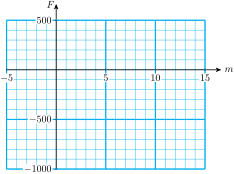
\includegraphics[width=\linewidth]{images/act-2-3-4.png}
\end{sbspanel}%
\end{sidebyside}%
\par
Use your graph to answer the questions below, and label the point on the graph that gives the answer.%
\item{}What will Francine's financial status be 7 months from now?%
\item{}When was Francine's financial status \(-\)\textdollar{}900?%
\end{enumerate}
%
\end{enumerate}
%
\end{activity}
\end{introduction}%
%
%
\typeout{************************************************}
\typeout{Subsubsection  Wrap-Up}
\typeout{************************************************}
%
\begin{subsubsectionptx}{Wrap-Up}{}{Wrap-Up}{}{}{g:subsubsection:idm46056765057552}
\begin{objectives}{Objectives}{g:objectives:idm46056765084768}
In this Lesson we practiced the following skills:%
%
\begin{itemize}[label=\textbullet]
\item{}Graphing a linear equation%
\item{}Plotting points on a Cartesian coordinate system%
\item{}Using a graph to answer questions about a model%
\end{itemize}
\end{objectives}
Questions to answer before the Homework Preview.%
\begin{outcomes}{Questions}{g:outcomes:idm46056765108464}
%
\begin{enumerate}[label=\arabic*]
\item{}In Activity 1, what are the intervals represented by each grid line on the axes?%
\item{}In Activity 2, what is the \(x\)-coordinate of the point with \(y\)-coordinate 16?%
\item{}In Activity 3, problem 2, if you increase the value of \(m\), does \(F\) increase or decrease?%
\end{enumerate}
\end{outcomes}
\end{subsubsectionptx}
\end{subsectionptx}
%
%
\typeout{************************************************}
\typeout{Subsection  Homework Preview}
\typeout{************************************************}
%
\begin{subsectionptx}{Homework Preview}{}{Homework Preview}{}{}{g:subsection:idm46056765259248}
Here are exercises to try before the end of the class meeting.%
%
%
\typeout{************************************************}
\typeout{Exercises  Exercises}
\typeout{************************************************}
%
\begin{exercises-subsubsection}{Exercises}{}{Exercises}{}{}{g:exercises:idm46056765353360}
\par\medskip\noindent%
%
Complete the table of values and graph the equation.%
\begin{exercisegroupcol}{2}
\begin{divisionexerciseegcol}{1}{}{}{g:exercise:idm46056765647328}%
\(~~y=4-2x\)%
\begin{sidebyside}{1}{0}{0}{0}%
\begin{sbspanel}{1}%
{\centering%
{\tabularfont%
\begin{tabular}{AcAcAcAcAcA}\hrulethick
\(x\)&\(-3\)&\(0\)&\(2\)&\(5\)\tabularnewline\hrulethin
\(y\)&\(\hphantom{0000}\)&\(\hphantom{0000}\)&\(\hphantom{0000}\)&\(\hphantom{0000}\)\tabularnewline\hrulethin
\end{tabular}
}%
\par}
\end{sbspanel}%
\end{sidebyside}%
\begin{sidebyside}{1}{0.05}{0.05}{0}%
\begin{sbspanel}{0.9}%
\includegraphics[width=\linewidth]{images/pre-2-3-1.png}
\end{sbspanel}%
\end{sidebyside}%
\end{divisionexerciseegcol}%
\begin{divisionexerciseegcol}{2}{}{}{g:exercise:idm46056766749424}%
\(~~y=-6+3x\)%
\begin{sidebyside}{1}{0}{0}{0}%
\begin{sbspanel}{1}%
{\centering%
{\tabularfont%
\begin{tabular}{AcAcAcAcAcA}\hrulethick
\(x\)&\(-1\)&\(0\)&\(2\)&\(4\)\tabularnewline\hrulethin
\(y\)&\(\hphantom{0000}\)&\(\hphantom{0000}\)&\(\hphantom{0000}\)&\(\hphantom{0000}\)\tabularnewline\hrulethin
\end{tabular}
}%
\par}
\end{sbspanel}%
\end{sidebyside}%
\begin{sidebyside}{1}{0.05}{0.05}{0}%
\begin{sbspanel}{0.9}%
\includegraphics[width=\linewidth]{images/pre-2-3-1.png}
\end{sbspanel}%
\end{sidebyside}%
\end{divisionexerciseegcol}%
\begin{divisionexerciseegcol}{3}{}{}{g:exercise:idm46056767310672}%
\(~~y=-2+\dfrac{4}{3}x\)%
\begin{sidebyside}{1}{0}{0}{0}%
\begin{sbspanel}{1}%
{\centering%
{\tabularfont%
\begin{tabular}{AcAcAcAcAcA}\hrulethick
\(x\)&\(-3\)&\(0\)&\(3\)&\(6\)\tabularnewline\hrulethin
\(y\)&\(\hphantom{0000}\)&\(\hphantom{0000}\)&\(\hphantom{0000}\)&\(\hphantom{0000}\)\tabularnewline\hrulethin
\end{tabular}
}%
\par}
\end{sbspanel}%
\end{sidebyside}%
\begin{sidebyside}{1}{0.05}{0.05}{0}%
\begin{sbspanel}{0.9}%
\includegraphics[width=\linewidth]{images/pre-2-3-1.png}
\end{sbspanel}%
\end{sidebyside}%
\end{divisionexerciseegcol}%
\begin{divisionexerciseegcol}{4}{}{}{g:exercise:idm46056768040912}%
\(~~y=2-\dfrac{3}{4}x\)%
\begin{sidebyside}{1}{0}{0}{0}%
\begin{sbspanel}{1}%
{\centering%
{\tabularfont%
\begin{tabular}{AcAcAcAcAcA}\hrulethick
\(x\)&\(-8\)&\(-4\)&\(0\)&\(8\)\tabularnewline\hrulethin
\(y\)&\(\hphantom{0000}\)&\(\hphantom{0000}\)&\(\hphantom{0000}\)&\(\hphantom{0000}\)\tabularnewline\hrulethin
\end{tabular}
}%
\par}
\end{sbspanel}%
\end{sidebyside}%
\begin{sidebyside}{1}{0.05}{0.05}{0}%
\begin{sbspanel}{0.9}%
\includegraphics[width=\linewidth]{images/pre-2-3-1.png}
\end{sbspanel}%
\end{sidebyside}%
\end{divisionexerciseegcol}%
\end{exercisegroupcol}
\par\medskip\noindent
\end{exercises-subsubsection}
%
%
\typeout{************************************************}
\typeout{Solutions  Answers to Homework Preview}
\typeout{************************************************}
%
\begin{solutions-subsubsection}{Answers to Homework Preview}{}{Answers to Homework Preview}{}{}{g:solutions:idm46056770969760}
\begin{conclusion}{}%
%
\begin{multicols}{2}
\begin{enumerate}[label=\arabic*]
\item{}\begin{sidebyside}{1}{0.25}{0.25}{0}%
\begin{sbspanel}{0.5}%
\includegraphics[width=\linewidth]{images/pre-2-3-2.png}
\end{sbspanel}%
\end{sidebyside}%
%
\item{}\begin{sidebyside}{1}{0.25}{0.25}{0}%
\begin{sbspanel}{0.5}%
\includegraphics[width=\linewidth]{images/pre-2-3-3.png}
\end{sbspanel}%
\end{sidebyside}%
%
\item{}\begin{sidebyside}{1}{0.25}{0.25}{0}%
\begin{sbspanel}{0.5}%
\includegraphics[width=\linewidth]{images/pre-2-3-4.png}
\end{sbspanel}%
\end{sidebyside}%
%
\item{}\begin{sidebyside}{1}{0.25}{0.25}{0}%
\begin{sbspanel}{0.5}%
\includegraphics[width=\linewidth]{images/pre-2-3-5.png}
\end{sbspanel}%
\end{sidebyside}%
%
\end{enumerate}
\end{multicols}
%
\end{conclusion}%
\end{solutions-subsubsection}
\end{subsectionptx}
%
%
\typeout{************************************************}
\typeout{Exercises  Homework 2.3}
\typeout{************************************************}
%
\begin{exercises-subsection}{Homework 2.3}{}{Homework 2.3}{}{}{g:exercises:idm46056768485264}
\par\medskip\noindent%
%
For Problems 1\textendash{}2, the figure shown is the graph of an equation. Decide which of the given points are solutions of the equation.%
\begin{exercisegroupcol}{2}
\begin{divisionexerciseegcol}{1}{}{}{g:exercise:idm46056768699200}%
%
\begin{multicols}{2}
\begin{enumerate}[label=\alph*]
\item{}\(\displaystyle (2,0)\)%
\item{}\(\displaystyle (3,2)\)%
\item{}\(\displaystyle (-1,-2)\)%
\item{}\(\displaystyle (-3,-6)\)%
\end{enumerate}
\end{multicols}
%
\begin{sidebyside}{1}{0.125}{0.125}{0}%
\begin{sbspanel}{0.75}%
\resizebox{\linewidth}{!}{%
\tikzset{%
}
\begin{tikzpicture} [scale=.5]
\coordinate (O) at (0,0);
\draw[cyan] (-6,-6) grid (6,6);
\draw[black,thick, ->, >=stealth'] (-6,0)--(6.6,0) node[right]{$x$};
\draw[black,thick, ->, >=stealth'] (0,-6)--(0,6.6) node[left, xshift=2]{$y$};
\foreach \x in  {-5, 5} {
 \draw[cyan, very thick] (\x,-6) --++(0,12);
 \draw[cyan, very thick] (-6,\x) --++(12,0);
 \draw[black] (\x,.1) --++(0,-.2)  node[below, yshift=-2, fill=white, inner sep=1]   {$\x$};
 \draw[black] (.1,\x) --++(-.2,0)  node[left, xshift=-2, fill=white, inner sep=1]   {$\x$};
}
\draw[red, very thick, <->, >=stealth'] (-3,-6)--(6,6);
\end{tikzpicture}
}%
\end{sbspanel}%
\end{sidebyside}%
\end{divisionexerciseegcol}%
\begin{divisionexerciseegcol}{2}{}{}{g:exercise:idm46056777085392}%
%
\begin{multicols}{2}
\begin{enumerate}[label=\alph*]
\item{}\(\displaystyle (4,-2)\)%
\item{}\(\displaystyle (4,4)\)%
\item{}\(\displaystyle (0,4)\)%
\item{}\(\displaystyle (-1,-4)\)%
\end{enumerate}
\end{multicols}
%
\begin{sidebyside}{1}{0.125}{0.125}{0}%
\begin{sbspanel}{0.75}%
\resizebox{\linewidth}{!}{%
\tikzset{%
}
\begin{tikzpicture} [scale=.5]
\coordinate (O) at (0,0);
\draw[cyan] (-6,-6) grid (6,6);
\draw[black,thick, ->, >=stealth'] (-6,0)--(6.6,0) node[right]{$x$};
\draw[black,thick, ->, >=stealth'] (0,-6)--(0,6.6) node[left, xshift=2]{$y$};
\foreach \x in  {-5, 5} {
 \draw[cyan, very thick] (\x,-6) --++(0,12);
 \draw[cyan, very thick] (-6,\x) --++(12,0);
 \draw[black] (\x,.1) --++(0,-.2)  node[below, yshift=-2, fill=white, inner sep=1]   {$\x$};
 \draw[black] (.1,\x) --++(-.2,0)  node[left, xshift=-2, fill=white, inner sep=1]   {$\x$};
}
\draw[red, very thick, <->, >=stealth'] (4,-6)--(4,6);
\end{tikzpicture}
}%
\end{sbspanel}%
\end{sidebyside}%
\end{divisionexerciseegcol}%
\end{exercisegroupcol}
\par\medskip\noindent
\par\medskip\noindent%
%
For Problems 3\textendash{}5, give the coordinates of the labeled points.%
\begin{exercisegroupcol}{2}
\begin{divisionexerciseegcol}{3}{}{}{g:exercise:idm46056777079216}%
\begin{sidebyside}{1}{0}{0}{0}%
\begin{sbspanel}{1}%
\resizebox{\linewidth}{!}{%
\tikzset{%
}
\begin{tikzpicture} [scale=.3]
\coordinate (O) at (0,0);
\draw[cyan] (-10,-10) grid (10,10);
\draw[black,thick, ->, >=stealth'] (-10,0)--(11.6,0) node[right]{$x$};
\draw[black,thick, ->, >=stealth'] (0,-10)--(0,11.6) node[left, xshift=2]{$y$};
\foreach \x in  {-5, 5, -10, 10} {
 \draw[cyan, very thick] (\x,-10) --++(0,20);
 \draw[cyan, very thick] (-10,\x) --++(20,0);
 \draw[black] (\x,.15) --++(0,-.3)  node[below, yshift=-2, fill=white, inner sep=1]   {$\x$};
 \draw[black] (.15,\x) --++(-.3,0)  node[left, xshift=-2, fill=white, inner sep=1]   {$\x$};
}
\filldraw[red]  (-6,2) circle (2mm) node[above, yshift=3, fill=white, inner sep=1, text=black] {(a)}; 
\filldraw[red]  (-5,-7) circle (2mm) node[above, yshift=3, fill=white, inner sep=1, text=black] {(b)}; 
\filldraw[red]  (8,-4) circle (2mm) node[above, yshift=3, fill=white, inner sep=1, text=black] {(c)}; 
\filldraw[red]  (1,7) circle (2mm) node[above, xshift=1, yshift=3, fill=white, inner sep=1, text=black] {(d)}; 
\filldraw[red]  (0,-9) circle (2mm) node[right, xshift=3, fill=white, inner sep=1, text=black] {(e)}; 
\filldraw[red]  (-2,0) circle (2mm) node[above, yshift=3, fill=white, inner sep=1, text=black] {(f)}; 
\end{tikzpicture}
}%
\end{sbspanel}%
\end{sidebyside}%
\end{divisionexerciseegcol}%
\begin{divisionexerciseegcol}{4}{}{}{g:exercise:idm46056769110128}%
\begin{sidebyside}{1}{0}{0}{0}%
\begin{sbspanel}{1}%
\resizebox{\linewidth}{!}{%
\tikzset{%
}
\begin{tikzpicture} [scale=.3]
\coordinate (O) at (0,0);
\draw[cyan] (-10,-10) grid (10,10);
\draw[black,thick, ->, >=stealth'] (-10,0)--(11.6,0) node[right]{$x$};
\draw[black,thick, ->, >=stealth'] (0,-10)--(0,11.6) node[left, xshift=2]{$y$};
\foreach \x in  {-5, 5, -10, 10} {
 \draw[cyan, very thick] (\x,-10) --++(0,20);
 \draw[cyan, very thick] (-10,\x) --++(20,0);
 \draw[black] (\x,.15) --++(0,-.3)  node[below, yshift=-2, fill=white, inner sep=1]   {$\x$};
 \draw[black] (.15,\x) --++(-.3,0)  node[left, xshift=-2, fill=white, inner sep=1]   {$\x$};
}
\draw[blue, very thick] (-10,0)--(10,-10);
\filldraw[red]  (-10,0) circle (2mm) node[above, xshift=1, yshift=4, fill=white, inner sep=1, text=black] {(a)}; 
\filldraw[red]  (-2,-4) circle (2mm) node[above, xshift=1, yshift=4, fill=white, inner sep=1, text=black] {(b)}; 
\filldraw[red]  (0,-5) circle (2mm) node[below, yshift=-4, fill=white, inner sep=1, text=black] {(c)}; 
\filldraw[red]  (2,-6) circle (2mm) node[above, xshift=2, yshift=4, fill=white, inner sep=1, text=black] {(d)}; 
\filldraw[red]  (10,-10) circle (2mm) node[above, xshift=1, yshift=4, fill=white, inner sep=1, text=black] {(e)}; 
\end{tikzpicture}
}%
\end{sbspanel}%
\end{sidebyside}%
\end{divisionexerciseegcol}%
\begin{divisionexerciseegcol}{5}{}{}{g:exercise:idm46056769241440}%
\begin{sidebyside}{1}{0}{0}{0}%
\begin{sbspanel}{1}%
\resizebox{\linewidth}{!}{%
\tikzset{%
}
\begin{tikzpicture} [scale=.3]
\coordinate (O) at (0,0);
\draw[cyan] (0,-12) grid (20,8);
\draw[black,thick, ->, >=stealth'] (0,0)--(21.6,0) node[right]{$d$};
\draw[black,thick, ->, >=stealth'] (0,-12)--(0,9.6) node[left, xshift=2]{$P$};
\foreach \x in  {5, 10, 15, 20} {
 \draw[cyan, very thick] (\x,-12) --++(0,20);
 \draw[black] (\x,.15) --++(0,-.3)  node[below, yshift=-2, fill=white, inner sep=1]   {$\x$};
}
\foreach \y [evaluate=\y as \yi using int( 50* \y )] in {-12, -8, -4, 4, 8} {
 \draw[cyan, very thick] (0,\y) --++(20,0);
 \draw[black] (.15,\y) --++(-.3,0)  node[left, xshift=-2, fill=white, inner sep=1]   {$\yi$};
}
\draw[blue, very thick] (0,-12)--(20,4);
\filldraw[red]  (0,-12) circle (2mm) node[above, xshift=-1, yshift=6, fill=white, inner sep=1, text=black] {(a)}; 
\filldraw[red]  (10,-4) circle (2mm) node[above, xshift=-5, yshift=3, fill=white, inner sep=1, text=black] {(b)}; 
\filldraw[red]  (15,0) circle (2mm) node[above, xshift=-5, yshift=3, fill=white, inner sep=1, text=black] {(c)}; 
\filldraw[red]  (20,4) circle (2mm) node[above, xshift=-3, yshift=5, fill=white, inner sep=1, text=black] {(d)}; 
\end{tikzpicture}
}%
\end{sbspanel}%
\end{sidebyside}%
\end{divisionexerciseegcol}%
\end{exercisegroupcol}
\par\medskip\noindent
\par\medskip\noindent%
%
For Problems 6\textendash{}7,%
\begin{enumerate}[label=\alph*]
\item{}Write an equation relating the variables.%
\item{}Complete the table of values.%
\item{}Graph your equation on the grid.%
\end{enumerate}
%
\begin{exercisegroup}
\begin{divisionexerciseeg}{6}{}{}{g:exercise:idm46056769535456}%
Greta's math notebook has 100 pages, and she uses on average 6 pages per day for notes and homework.  How many pages, \(P\), will she have left after \(d\) days?%
\begin{sidebyside}{1}{0}{0}{0}%
\begin{sbspanel}{1}%
{\centering%
{\tabularfont%
\begin{tabular}{AcAcAcAcAcAcA}\hrulethick
\(d\)&\(0\)&\(2\)&\(5\)&\(10\)&\(15\)\tabularnewline\hrulethin
\(P\)&\(\hphantom{0000}\)&\(\hphantom{0000}\)&\(\hphantom{0000}\)&\(\hphantom{0000}\)&\(\hphantom{0000}\)\tabularnewline\hrulethin
\end{tabular}
}%
\par}
\end{sbspanel}%
\end{sidebyside}%
\begin{sidebyside}{1}{0.25}{0.25}{0}%
\begin{sbspanel}{0.5}%
\resizebox{\linewidth}{!}{%
\tikzset{%
}
\begin{tikzpicture} [xscale=.35, yscale=.09]
\coordinate (O) at (0,0);
\draw[cyan] (O) grid[xstep=2, ystep=5] (20,100);
\draw[black,thick, ->, >=stealth'] (O)--(21.6,0) node[right]{$d$};
\draw[black,thick, ->, >=stealth'] (O)--(0,106) node[left, xshift=2]{$P$};
\foreach \x in  {10,20} {
 \draw[black] (\x,.6) --++(0,-1.2)  node[below, yshift=-2, fill=white, inner sep=1]   {$\x$};
}
\foreach \x in  {10,20,...,100} {
 \draw[black] (.2,\x) --++(-.4,0)  node[left, xshift=-2, fill=white, inner sep=1]   {$\x$};
}
\node[below left, xshift=1] at (O) {0};
\end{tikzpicture}
}%
\end{sbspanel}%
\end{sidebyside}%
\end{divisionexerciseeg}%
\begin{divisionexerciseeg}{7}{}{}{g:exercise:idm46056777074960}%
Delbert shares a house with four roommates. He pays \textdollar{}200 rent per month, plus his share of the utilities. If the utilities cost \(U\) dollars, how much money, \(M\), does Delbert owe?%
\begin{sidebyside}{1}{0}{0}{0}%
\begin{sbspanel}{1}%
{\centering%
{\tabularfont%
\begin{tabular}{AcAcAcAcAcAcA}\hrulethick
\(U\)&\(20\)&\(40\)&\(80\)&\(100\)&\(200\)\tabularnewline\hrulethin
\(M\)&\(\hphantom{0000}\)&\(\hphantom{0000}\)&\(\hphantom{0000}\)&\(\hphantom{0000}\)&\(\hphantom{0000}\)\tabularnewline\hrulethin
\end{tabular}
}%
\par}
\end{sbspanel}%
\end{sidebyside}%
\begin{sidebyside}{1}{0.25}{0.25}{0}%
\begin{sbspanel}{0.5}%
\resizebox{\linewidth}{!}{%
\tikzset{%
}
\begin{tikzpicture} [scale=.03]
\coordinate (O) at (0,0);
\draw[cyan] (O) grid[xstep=20, ystep=10] (200,260);
\draw[black,thick, ->, >=stealth'] (O)--(215,0) node[right]{$U$};
\draw[black,thick, ->, >=stealth'] (O)--(0,275) node[left, xshift=2]{$M$};
\foreach \x in  {100,200} {
 \draw[cyan,very thick] (\x,0) --++(0,260); 
 \draw[black] (\x,2) --++(0,-4)  node[below, yshift=-2, fill=white, inner sep=1]   {$\x$};
}
\foreach \x in  {50,100,...,250} {
 \draw[cyan, very thick] (0,\x) --++(200,0); 
 \draw[black] (2,\x) --++(-4,0)  node[left, xshift=-2, fill=white, inner sep=1]   {$\x$};
}
\node[below left, xshift=1] at (O) {0};
\end{tikzpicture}
}%
\end{sbspanel}%
\end{sidebyside}%
\end{divisionexerciseeg}%
\end{exercisegroup}
\par\medskip\noindent
\begin{divisionexercise}{8}{}{}{g:exercise:idm46056772168288}%
Darren inherited some money and has been spending it at the rate of \textdollar{}100 per day. Right now he has \textdollar{}2000 left.%
\begin{enumerate}[label=\alph*]
\item{}Write an equation for Darren's balance, \(B\), after \(d\) days.%
\item{}Fill in the table. Negative values of \(d\) represent days in the past.%
\begin{sidebyside}{1}{0}{0}{0}%
\begin{sbspanel}{1}%
{\centering%
{\tabularfont%
\begin{tabular}{AcAcAcAcAcAcAcAcA}\hrulethick
\(d\)&\(-15\)&\(-5\)&\(0\)&\(5\)&\(10\)&\(15\)&\(20\)\tabularnewline\hrulethin
\(B\)&\(\hphantom{0000}\)&\(\hphantom{0000}\)&\(\hphantom{0000}\)&\(\hphantom{0000}\)&\(\hphantom{0000}\)&\(\hphantom{0000}\)&\(\hphantom{0000}\)\tabularnewline\hrulethin
\end{tabular}
}%
\par}
\end{sbspanel}%
\end{sidebyside}%
\item{}Graph your equation, using the values in the table.%
\begin{sidebyside}{1}{0.3}{0.3}{0}%
\begin{sbspanel}{0.4}%
\resizebox{\linewidth}{!}{%
\tikzset{%
}
\begin{tikzpicture} [scale=.4]
\draw[cyan] (-4,-4) grid(10,10);
\draw[black,thick, ->, >=stealth'] (-4,0)--(11,0) node[right]{$d$};
\draw[black,thick, ->, >=stealth'] (0,-4)--(0,11) node[left, xshift=2]{$B$};
\foreach \x [evaluate=\x as \xi using int( 5* \x )] in  {-4,4,8} {
 \draw[cyan,very thick] (\x,-4) --(\x,10); 
 \draw[black] (\x,.2) --++(0,-.4)  node[below, yshift=-2, fill=white, inner sep=1]   {$\xi$};
}
\foreach \x [evaluate=\x as \xi using int( 500* \x )] in  {-4,4,8} {
 \draw[cyan, very thick] (-4,\x) --(10,\x); 
 \draw[black] (.2,\x) --++(-.4,0)  node[left, xshift=-2, fill=white, inner sep=1]   {$\xi$};
}
\end{tikzpicture}
}%
\end{sbspanel}%
\end{sidebyside}%
\par
Use your graph to answer the following questions:%
\item{}What was Darren's balance 15 days ago?%
\item{}When will Darren's balance reach \textdollar{}500?%
\end{enumerate}
%
\end{divisionexercise}%
\begin{divisionexercise}{9}{}{}{g:exercise:idm46056782893392}%
Gregory purchased stereo equipment on a monthly installment plan. After \(m\) months, Gregory still owes a balance of \(B\) dollars.%
\begin{sidebyside}{1}{0.3}{0.3}{0}%
\begin{sbspanel}{0.4}%
\resizebox{\linewidth}{!}{%
\tikzset{%
}
\begin{tikzpicture} [scale=.3]
\coordinate (O) at (0,0);
\draw[cyan] (O) grid(20,20);
\draw[black,thick, ->, >=stealth'] (O)--(22,0) node[right]{$m$};
\draw[black,thick, ->, >=stealth'] (O)--(0,22) node[left, xshift=2]{$B$};
\foreach \x in  {5,10,15, 20} {
 \draw[cyan,very thick] (\x,0) --(\x,20); 
 \draw[black] (\x,.2) --++(0,-.4)  node[below, yshift=-2, fill=white, inner sep=1]   {$\x$};
}
\foreach \x [evaluate=\x as \xi using int( 30* \x )] in  {5,10,15, 20} {
 \draw[cyan, very thick] (0,\x) --(20,\x); 
 \draw[black] (.2,\x) --++(-.4,0)  node[left, xshift=-2, fill=white, inner sep=1]   {$\xi$};
}
\draw[red, ultra thick] (0,18)--(18,0);
\node[below left, xshift=1] at (O) {0};
\end{tikzpicture}
}%
\end{sbspanel}%
\end{sidebyside}%
\par
%
\begin{enumerate}[label=\alph*]
\item{}What was the price of the stereo equipment?%
\item{}How much does Gregory pay each month?%
\item{}How much does Gregory owe after 6 months?%
\item{}How many monthly payments will Gregory make?%
\item{}Write an algebraic equation for \(B\) in terms of \(m\).%
\end{enumerate}
%
\end{divisionexercise}%
\par\medskip\noindent%
%
For part (c) of Problems 10\textendash{}11, write an equation and use your graph to solve it.%
\begin{exercisegroup}
\begin{divisionexerciseeg}{10}{}{}{g:exercise:idm46056782883744}%
On a 100-point test, Lori loses 5 points for each wrong answer.%
\begin{enumerate}[label=\alph*]
\item{}Write an equation for Lori's score, \(s\), if she gives \(x\) wrong answers.%
\item{}Complete the table of values and graph your equation.%
\begin{sidebyside}{1}{0}{0}{0}%
\begin{sbspanel}{1}%
{\centering%
{\tabularfont%
\begin{tabular}{AcAcAcAcAcA}\hrulethick
\(x\)&\(2\)&\(5\)&\(6\)&\(12\)\tabularnewline\hrulethin
\(s\)&\(\hphantom{0000}\)&\(\hphantom{0000}\)&\(\hphantom{0000}\)&\(\hphantom{0000}\)\tabularnewline\hrulethin
\end{tabular}
}%
\par}
\end{sbspanel}%
\end{sidebyside}%
\begin{sidebyside}{1}{0.25}{0.25}{0}%
\begin{sbspanel}{0.5}%
\resizebox{\linewidth}{!}{%
\tikzset{%
}
\begin{tikzpicture} [scale=.30]
\coordinate (O) at (0,0);
\draw[cyan] (O) grid[step=2] (20,20);
\draw[black,thick, ->, >=stealth'] (O)--(22,0) node[right]{$x$};
\draw[black,thick, ->, >=stealth'] (O)--(0,22) node[left, xshift=2]{$s$};
\foreach \x in  {10, 20} {
 \draw[cyan,very thick] (\x,0) --(\x,20); 
 \draw[black] (\x,.2) --++(0,-.4)  node[below, yshift=-2, fill=white, inner sep=1]   {$\x$};
}
\foreach \x [evaluate=\x as \xi using int( 5* \x )] in  {10,20} {
 \draw[cyan, very thick] (0,\x) --(20,\x); 
 \draw[black] (.2,\x) --++(-.4,0)  node[left, xshift=-2, fill=white, inner sep=1]   {$\xi$};
}
\node[below left, xshift=1] at (O) {0};
\end{tikzpicture}
}%
\end{sbspanel}%
\end{sidebyside}%
\item{}If Lori's score is 65, how many wrong answers did she give?%
\end{enumerate}
%
\end{divisionexerciseeg}%
\begin{divisionexerciseeg}{11}{}{}{g:exercise:idm46056783779472}%
The water in Silver Pond is 10 feet deep, but the water level is dropping at a rate of \(\dfrac{1}{2}\) inch per week.%
\begin{enumerate}[label=\alph*]
\item{}Write an equation for the depth, \(d\), of the pond after \(w\) weeks.%
\item{}Complete the table of values and graph your equation.%
\begin{sidebyside}{1}{0}{0}{0}%
\begin{sbspanel}{1}%
{\centering%
{\tabularfont%
\begin{tabular}{AcAcAcAcAcA}\hrulethick
\(w\)&\(24\)&\(36\)&\(84\)&\(120\)\tabularnewline\hrulethin
\(d\)&\(\hphantom{0000}\)&\(\hphantom{0000}\)&\(\hphantom{0000}\)&\(\hphantom{0000}\)\tabularnewline\hrulethin
\end{tabular}
}%
\par}
\end{sbspanel}%
\end{sidebyside}%
\begin{sidebyside}{1}{0.25}{0.25}{0}%
\begin{sbspanel}{0.5}%
\resizebox{\linewidth}{!}{%
\tikzset{%
}
\begin{tikzpicture} [scale=.50]
\coordinate (O) at (0,0);
\draw[cyan] (O) grid (10,12);
\draw[black,thick, ->, >=stealth'] (O)--(11,0) node[right]{$w$};
\draw[black,thick, ->, >=stealth'] (O)--(0,12.8) node[left, xshift=1]{$d$};
\foreach \x [evaluate=\x as \xi using int( 12* \x )]in  {2,4,6,8,10} {
 \draw[cyan,very thick] (\x,0) --(\x,12); 
 \draw[black] (\x,.2) --++(0,-.4)  node[below, yshift=-2, fill=white, inner sep=1]   {$\xi$};
}
\foreach \x [evaluate=\x as \xi using int( 10* \x )] in  {5,10} {
 \draw[cyan, very thick] (0,\x) --(10,\x); 
 \draw[black] (.2,\x) --++(-.4,0)  node[left, xshift=-2, fill=white, inner sep=1]   {$\xi$};
}
\node[below left, xshift=1] at (O) {0};
\end{tikzpicture}
}%
\end{sbspanel}%
\end{sidebyside}%
\item{}How long will it take until the depth of the pond is 8 feet? (Hint: Convert all the units to inches.)%
\end{enumerate}
%
\end{divisionexerciseeg}%
\end{exercisegroup}
\par\medskip\noindent
\par\medskip\noindent%
%
For Problems 12\textendash{}15, choose four \(x\)-values and make a table of values, then graph the equation. Extend your line far enough that it crosses both axes.%
\begin{exercisegroupcol}{2}
\begin{divisionexerciseegcol}{12}{}{}{g:exercise:idm46056785372480}%
\(y=x+3\)%
\begin{sidebyside}{1}{0}{0}{0}%
\begin{sbspanel}{1}%
\resizebox{\linewidth}{!}{%
\tikzset{%
}
\begin{tikzpicture} [scale=.3]
\coordinate (O) at (0,0);
\draw[cyan] (-10,-10) grid (10,10);
\draw[black,thick, ->, >=stealth'] (-10,0)--(11.6,0) node[right]{$x$};
\draw[black,thick, ->, >=stealth'] (0,-10)--(0,11.6) node[left, xshift=2]{$y$};
\foreach \x in  {-5, 5, -10, 10} {
 \draw[cyan, very thick] (\x,-10) --++(0,20);
 \draw[cyan, very thick] (-10,\x) --++(20,0);
 \draw[black] (\x,.15) --++(0,-.3)  node[below, yshift=-2, fill=white, inner sep=1]   {$\x$};
 \draw[black] (.15,\x) --++(-.3,0)  node[left, xshift=-2, fill=white, inner sep=1]   {$\x$};
}
\end{tikzpicture}
}%
\end{sbspanel}%
\end{sidebyside}%
\end{divisionexerciseegcol}%
\begin{divisionexerciseegcol}{13}{}{}{g:exercise:idm46056785369376}%
\(y=2x+1\)%
\begin{sidebyside}{1}{0}{0}{0}%
\begin{sbspanel}{1}%
\includegraphics[width=\linewidth]{images/hp-2-3-12}
\end{sbspanel}%
\end{sidebyside}%
\end{divisionexerciseegcol}%
\begin{divisionexerciseegcol}{14}{}{}{g:exercise:idm46056785365328}%
\(y=-\dfrac{1}{2}x-5\)%
\begin{sidebyside}{1}{0}{0}{0}%
\begin{sbspanel}{1}%
\includegraphics[width=\linewidth]{images/hp-2-3-12}
\end{sbspanel}%
\end{sidebyside}%
\end{divisionexerciseegcol}%
\begin{divisionexerciseegcol}{15}{}{}{g:exercise:idm46056785363456}%
\(y=\dfrac{5}{4}x-4\)%
\begin{sidebyside}{1}{0}{0}{0}%
\begin{sbspanel}{1}%
\includegraphics[width=\linewidth]{images/hp-2-3-12}
\end{sbspanel}%
\end{sidebyside}%
\end{divisionexerciseegcol}%
\end{exercisegroupcol}
\par\medskip\noindent
\begin{divisionexercise}{16}{}{}{g:exercise:idm46056785359408}%
The graph of \(y=2x+6\) is shown below.%
\begin{sidebyside}{1}{0.275}{0.275}{0}%
\begin{sbspanel}{0.45}%
\resizebox{\linewidth}{!}{%
\tikzset{%
}
\begin{tikzpicture} [scale=.3]
\coordinate (O) at (0,0);
\draw[cyan] (-10,-10) grid (10,10);
\draw[black,thick, ->, >=stealth'] (-10,0)--(11.6,0) node[right]{$x$};
\draw[black,thick, ->, >=stealth'] (0,-10)--(0,11.6) node[left, xshift=2]{$y$};
\foreach \x in  {-5, 5, -10, 10} {
 \draw[cyan, very thick] (\x,-10) --++(0,20);
 \draw[cyan, very thick] (-10,\x) --++(20,0);
 \draw[black] (\x,.15) --++(0,-.3)  node[below, yshift=-2, fill=white, inner sep=1]   {$\x$};
 \draw[black] (.15,\x) --++(-.3,0)  node[left, xshift=-2, fill=white, inner sep=1]   {$\x$};
}
\draw[red,very thick, <->, >=stealth'] (-8,-10)--(2,10);
\end{tikzpicture}
}%
\end{sbspanel}%
\end{sidebyside}%
\par
%
\begin{enumerate}[label=\alph*]
\item{}Use the graph to evaluate the expression \(2x+6\) for \(x=-5\).%
\item{}Find a point on the graph with \(y=-4\).  What is the \(x\)-value of the point?%
\item{}Verify that the coordinates of your point in part (b) satisfy the equation of the graph.%
\item{}Use the graph to find an \(x\)-value that produces a \(y\)-value of 8.%
\item{}Find two points on the graph for which \(y \gt -4\).  What are their \(x\)-values?%
\end{enumerate}
%
\end{divisionexercise}%
\par\medskip\noindent%
%
For Problems 17\textendash{}18, use the graph to solve the equations. Show your solutions on the graph. Then check your solutions algebraically.%
\begin{exercisegroupcol}{2}
\begin{divisionexerciseegcol}{17}{}{}{g:exercise:idm46056784001424}%
\begin{sidebyside}{1}{0}{0}{0}%
\begin{sbspanel}{1}%
\resizebox{\linewidth}{!}{%
\tikzset{%
}
\begin{tikzpicture} [xscale=.1, yscale=.4]
\coordinate (O) at (0,0);
\draw[cyan] (-48,-12) grid[xstep=4] (12,2);
\draw[black,thick, ->, >=stealth'] (-48,0)--(15,0) node[right]{$x$};
\draw[black,thick, ->, >=stealth'] (0,-12)--(0,3) node[left, xshift=2]{$y$};
\foreach \x in  {-48,-36,-24,-12,12} {
 \draw[cyan, very thick] (\x,-12) --(\x,2);
 \draw[black] (\x,.15) --++(0,-.3)  node[below, yshift=-5, fill=white, inner sep=1]   {$\x$};
}
\foreach \x in  {-5,-10} {
 \draw[cyan, very thick] (-48,\x) --(12,\x);
 \draw[black] (.15,\x) --++(-.3,0)  node[left, xshift=-4, fill=white, inner sep=1]   {$\x$};
}
\draw[red,very thick, <->, >=stealth'] (-44,2)--(12,-12);
\node[below, text=red,fill=white, inner sep=2] at (-36,-10.5) {$y=9-\frac{x}{4}$};
\end{tikzpicture}
}%
\end{sbspanel}%
\end{sidebyside}%
\par
%
\begin{enumerate}[label=\alph*]
\item{}\(\displaystyle -9-\dfrac{x}{4}=-5\)%
\item{}\(\displaystyle -9-\dfrac{x}{4}=1\)%
\end{enumerate}
%
\end{divisionexerciseegcol}%
\begin{divisionexerciseegcol}{18}{}{}{g:exercise:idm46056783995808}%
\begin{sidebyside}{1}{0.05}{0.05}{0}%
\begin{sbspanel}{0.9}%
\resizebox{\linewidth}{!}{%
\tikzset{%
}
\begin{tikzpicture} [xscale=.25, yscale=.5]
\draw[cyan] (-4,-4) grid[xstep=2] (16,7);
\draw[black,thick, ->, >=stealth'] (-4,0)--(18,0) node[right]{$x$};
\draw[black,thick, ->, >=stealth'] (0,-4)--(0,8) node[left, xshift=2]{$y$};
\foreach \x in  {-4,10} {
 \draw[cyan, very thick] (\x,-4) --(\x,7);
 \draw[black] (\x,.15) --++(0,-.3)  node[below, yshift=-5, fill=white, inner sep=1]   {$\x$};
}
\foreach \x in  {-3,5} {
 \draw[cyan, very thick] (-4,\x) --(16,\x);
 \draw[black] (.15,\x) --++(-.3,0)  node[left, xshift=-4, fill=white, inner sep=1]   {$\x$};
}
\draw[red,very thick, <->, >=stealth'] (0,7)--(16,{7-32/3});
\node[below, text=red,fill=white, inner sep=2] at (11,6.5) {$y=7-\frac{2x}{3}$};
\end{tikzpicture}
}%
\end{sbspanel}%
\end{sidebyside}%
\par
%
\begin{enumerate}[label=\alph*]
\item{}\(\displaystyle 7-\dfrac{2x}{3}=3\)%
\item{}\(\displaystyle 7-\dfrac{2x}{3}=11\)%
\end{enumerate}
%
\end{divisionexerciseegcol}%
\end{exercisegroupcol}
\par\medskip\noindent
\par\medskip\noindent%
%
For Problems 19\textendash{}20, use the graph to estimate the solution of the equation. Then use a calculator to help you verify the solution algebraically. Do you think your estimate was too big or too small?%
\begin{exercisegroupcol}{2}
\begin{divisionexerciseegcol}{19}{}{}{g:exercise:idm46056777362064}%
\(37.21-8.4t=24.61\)%
\begin{sidebyside}{1}{0.025}{0.025}{0}%
\begin{sbspanel}{0.95}%
\resizebox{\linewidth}{!}{%
\tikzset{%
}
\begin{tikzpicture} [xscale=.55, yscale=.055]
\draw[cyan] (-6,-20) grid[ystep=10] (6,80);
\draw[black,thick, ->, >=stealth'] (-6,0)--(7,0) node[right]{$t$};
\draw[black,thick, ->, >=stealth'] (0,-20)--(0,85) node[left, xshift=2]{$y$};
\foreach \x in  {-4,4} {
 \draw[cyan, very thick] (\x,-20) --(\x,80);
 \draw[black] (\x,1.5) --++(0,-3)  node[below, yshift=-5, fill=white, inner sep=1]   {$\x$};
}
\foreach \x in  {-20,30,60} {
 \draw[cyan, very thick] (-6,\x) --(6,\x);
 \draw[black] (.15,\x) --++(-.3,0)  node[left, xshift=-4, fill=white, inner sep=1]   {$\x$};
}
\draw[red,very thick, <->, >=stealth'] ({(80-37.21)/(-8.4)},80)--(6,{37.21-8.4*6});
\node[below, text=red,fill=white, inner sep=2] at (3,70) {$37.21-8.4t=y$};
\end{tikzpicture}
}%
\end{sbspanel}%
\end{sidebyside}%
\end{divisionexerciseegcol}%
\begin{divisionexerciseegcol}{20}{}{}{g:exercise:idm46056785246576}%
\(-26.4=-3.65+9.1x\)%
\begin{sidebyside}{1}{0.05}{0.05}{0}%
\begin{sbspanel}{0.9}%
\resizebox{\linewidth}{!}{%
\tikzset{%
}
\begin{tikzpicture} [xscale=.6, yscale=.06]
\draw[cyan] (-5,-50) grid[ystep=10] (5,50);
\draw[black,thick, ->, >=stealth'] (-5,0)--(6,0) node[right]{$x$};
\draw[black,thick, ->, >=stealth'] (0,-50)--(0,60) node[left, xshift=2]{$y$};
\foreach \x in  {-5,5} {
 \draw[cyan, very thick] (\x,-50) --(\x,50);
 \draw[black] (\x,1.5) --++(0,-3)  node[below, yshift=-5, fill=white, inner sep=1]   {$\x$};
}
\foreach \x in  {-50,50} {
 \draw[cyan, very thick] (-5,\x) --(5,\x);
 \draw[black] (.15,\x) --++(-.3,0)  node[left, xshift=-4, fill=white, inner sep=1]   {$\x$};
}
\draw[red,very thick, <->, >=stealth'] (5,{-3.65+9.1*5})--(-5,{-3.65+9.1*-5});
\node[below, text=red,fill=white, inner sep=2] at (2.5,-37) {$y=3.65+9.1x$};
\end{tikzpicture}
}%
\end{sbspanel}%
\end{sidebyside}%
\end{divisionexerciseegcol}%
\end{exercisegroupcol}
\par\medskip\noindent
\end{exercises-subsection}
\end{sectionptx}
%
%
\typeout{************************************************}
\typeout{Section 2.4 Linear Equations and Inequalities}
\typeout{************************************************}
%
\begin{sectionptx}{Linear Equations and Inequalities}{}{Linear Equations and Inequalities}{}{}{x:section:Linear-Equations-and-Inequalities}
%
%
\typeout{************************************************}
\typeout{Subsection  Solving Equations}
\typeout{************************************************}
%
\begin{subsectionptx}{Solving Equations}{}{Solving Equations}{}{}{g:subsection:idm46056774660832}
\index{solving an equation}%
\index{equation!solving}%
\begin{introduction}{}%
We solve an equation by isolating the variable on one side of the equation. If an equation involves two or more operations, we must undo those operations in reverse order.%
\begin{example}{}{x:example:Example-2-4-1}%
The equation%
\begin{equation*}
T=50+15u
\end{equation*}
describes college tuition consisting of a \textdollar{}50 registration fee plus \textdollar{}15 per unit. How many units can you take if you have \textdollar{}290 saved for tuition?%
\par\smallskip%
\noindent\textbf{\blocktitlefont Solution}.\hypertarget{g:solution:idm46056774812656}{}\quad{}We can answer the question by solving the equation%
\begin{equation*}
\alert{290}=50+15u
\end{equation*}
where we have substituted \textdollar{}290 for the tuition, \(T\). Think about the expression \(50+15u\). How would you evaluate this expression if you were given a value for \(u\)? Following the order of operations, you would%
\begin{align*}
\amp 1.~~~\text{First multiply by 15}\\
\amp 2.~~~\text{Then add 50}
\end{align*}
In order to solve the equation, we must reverse these two steps to undo the operations and isolate the variable.  We first subtract 50 from both sides of the equation:%
\begin{align*}
290 ~\amp = ~~~50+15u \amp \amp  \blert{\text{Subtract 50 from both sides.}}\\
\underline{\blert{-50}}  \amp = \underline{\blert{-50}}\\
240  ~\amp = ~~~~~~~~~~~~~15u
\end{align*}
This isolates the term that contains the variable, \(15u\). Then we divide both sides of the equation by 15.%
\begin{equation*}
\begin{aligned}
\dfrac{240}{\blert{15}} \amp = \dfrac{15u}{\blert{15}} \amp \amp \blert{\text{Divide both sides by 15.}}\\
16  \amp = u   
\end{aligned}
\end{equation*}
You can enroll in 16 units. We can check the solution by substituting 16 for \(u\) in the original equation.%
\begin{align*}
\blert{\text{Check:}}~~~~~~~~~~~~    50+15u =\amp 290\\
50+15(\alert{16}) =\amp 50+240=290 ~~~~~ \blert{\text{True}}
\end{align*}
Because a true statement results, the solution checks.%
\end{example}
\begin{assemblage}{Look Closer.}{g:assemblage:idm46056774647280}%
In \hyperref[x:example:Example-2-4-1]{Example~{\xreffont\ref{x:example:Example-2-4-1}}}, notice how we reversed the operations used in the equation.%
\begin{align*}
\amp \blert{\text{Operations performed on}~u} \amp \amp \blert{\text{Steps for solution}}\\
\amp 1.~~~\text{Multiply by 15}  \amp \amp 1.~~~\text{Subtract 50}\\
\amp 2.~~~\text{Add 50}  \amp \amp 2.~~~\text{Divide by 15}
\end{align*}
%
\end{assemblage}
\begin{assemblage}{Strategy for solving equations.}{g:assemblage:idm46056775431568}%
To solve an equation that involves two or more operations, we undo those operations in reverse order.%
\end{assemblage}
\begin{example}{}{x:example:Example-2-4-2}%
Solve \(~8-3x=-10\)%
\par\smallskip%
\noindent\textbf{\blocktitlefont Solution}.\hypertarget{g:solution:idm46056775536624}{}\quad{}The left side of the equation has two terms: \(8\) and \(-3x\). We want to isolate the term containing the variable, so we subtract 8 from both sides.%
\begin{align*}
8-3x \amp = -10 \amp \amp  \blert{\text{Subtract 8 from both sides.}}\\
\underline{\blert{-8}}  \amp =\underline{\blert{-8}}\\
-3x \amp = -18
\end{align*}
Next, we divide both sides by \(-3\) to get%
\begin{align*}
\dfrac{-3x}{\blert{-3}} \amp = \dfrac{-18}{\blert{-3}} \amp \amp \blert{\text{Divide both sides by}~-3.}\\
x \amp = 6
\end{align*}
The solutions is 6.%
\begin{equation*}
\blert{\text{Check:}}~~~~~~~~8-3(\alert{6})=8-18=-10
\end{equation*}
%
\end{example}
\begin{warning}{}{g:warning:idm46056775617584}%
In the second step of \hyperref[x:example:Example-2-4-2]{Example~{\xreffont\ref{x:example:Example-2-4-2}}}, the term \(-3x\) means "\(-3\) times \(x\)," so we divide both sides by \(-3\). Do not try to add 3 to both sides.%
\end{warning}
\end{introduction}%
%
%
\typeout{************************************************}
\typeout{Subsubsection  Reading Questions}
\typeout{************************************************}
%
\begin{subsubsectionptx}{Reading Questions}{}{Reading Questions}{}{}{g:subsubsection:idm46056775832560}
\begin{inlineexercise}{}{g:exercise:idm46056775990304}%
If an equation involves more than one operation, how must we undo those operations?%
\par\smallskip%
\noindent\textbf{\blocktitlefont Answer}.\hypertarget{g:answer:idm46056776004800}{}\quad{}In reverse order%
\end{inlineexercise}
\begin{inlineexercise}{}{g:exercise:idm46056776017168}%
Delbert says he solved the equation \(-5x=15\) by adding \(5\) to both sides. What is wrong with his method?%
\par\smallskip%
\noindent\textbf{\blocktitlefont Answer}.\hypertarget{g:answer:idm46056776076832}{}\quad{}He should divide by \(-5\).%
\end{inlineexercise}
\end{subsubsectionptx}
\end{subsectionptx}
%
%
\typeout{************************************************}
\typeout{Subsection  Applied Problems}
\typeout{************************************************}
%
\begin{subsectionptx}{Applied Problems}{}{Applied Problems}{}{}{g:subsection:idm46056775979520}
\index{applied problems}%
Problem solving often involves signed numbers, either in the equation that models the problem or in its solution, or both.%
\begin{example}{}{g:example:idm46056776164384}%
The trout population in Clear Lake is decreasing by approximately 60 fish per year, and this year there are about 430 trout in the lake. If the population drops to 100, the Park Service will have to restock the lake.%
\begin{enumerate}[label=\alph*]
\item{}Write an equation for the population \(P\) of trout \(x\) years from now.%
\item{}When will the Park Service have to restock the lake?%
\item{}Graph your equation for \(P\), and illustrate your answer to part (b) on the graph.%
\end{enumerate}
%
\par\smallskip%
\noindent\textbf{\blocktitlefont Solution}.\hypertarget{g:solution:idm46056776517376}{}\quad{}%
\begin{enumerate}[label=\alph*]
\item{}The population starts this year at 430, and decreases by 60 for each following year. Thus, \(P=430-60x\).%
\item{}We would like to find the value of \(x\) when \(P=100\). We substitute 100 for \(P\), and solve the equation for \(x\).%
\begin{align*}
100 ~~\amp = ~~~430-60x \amp \amp  \blert{\text{Subtract 430 from both sides.}}\\
\underline{\blert{-430}}  \amp = \underline{\blert{-430}}\\
-330 ~~\amp = -60x \\
\hphantom{0000}\\
\dfrac{-330}{\blert{-60}} \amp = \dfrac{-60x}{\blert{-60}} \amp \amp \blert{\text{Divide both sides by}~-60.}\\
5.5 \amp = x 
\end{align*}
The Park Service will have to restock the lake in five and a half years, if the population continues to decline at the current rate.%
\item{}The figure shows the graph of the equation \(P=430-60x\). To solve%
\begin{equation*}
100=430-60x
\end{equation*}
we locate the point on the graph with \(P=100\), and read its \(x\)-coordinate, at about 5.5.%
\begin{sidebyside}{1}{0.3}{0.3}{0}%
\begin{sbspanel}{0.4}%
\resizebox{\linewidth}{!}{%
\tikzset{%
}
\begin{tikzpicture} [xscale=.5, yscale=.018]
\coordinate (O) at (0,0);
\draw[cyan] (O) grid[ystep=20] (10,440);
\draw[black,thick, ->, >=stealth'] (O)--(11,0) node[right]{$x$};
\draw[black,thick, ->, >=stealth'] (O)--(0,460) node[left, xshift=2]{$P$};
\foreach \x in  {10} {
 \draw[cyan, very thick] (\x,0) --(\x,440);
 \draw[black] (\x,5) --++(0,-10)  node[below] {$\x$};
}
\draw[cyan, very thick] (5,0) --(5,440);
\foreach \x in  {200, 300, 400} {
 \draw[cyan, very thick] (0,\x) --(10,\x);
 \draw[black] (.15,\x) --++(-.3,0)  node[left] {$\x$};
}
\draw[cyan, thick] (0,100) --(10,100);
\draw[red,very thick, <->, >=stealth'] (0,430)--({43/6},0);
\node[below, text=red] at (5.5,0) {$5.5$};
\draw[black] (.15,100)--++(-.3,0) node[left, text=red] {$100$};
\filldraw[blue] (5.5,100) ellipse (.2cm and 6cm);
\foreach \x in {0,1,1,2.2,3.3,4.4}{
 \draw[black, very thick, ->,>=stealth'] (\x,100)--++(.8,0);
 }
\foreach \x in {89, 66, 43, 20}{
 \draw[black, very thick, ->,>=stealth'] (5.5, \x)--++(0, -20);
 }
\end{tikzpicture}
}%
\end{sbspanel}%
\end{sidebyside}%
\end{enumerate}
%
\end{example}
\end{subsectionptx}
%
%
\typeout{************************************************}
\typeout{Subsection  Solving Inequalities}
\typeout{************************************************}
%
\begin{subsectionptx}{Solving Inequalities}{}{Solving Inequalities}{}{}{g:subsection:idm46056777588112}
\index{solving an inequality}%
\index{inequality!solving}%
\begin{introduction}{}%
\begin{assemblage}{Inequality.}{g:assemblage:idm46056777526512}%
A statement that uses one of the symbols \(\gt\) or \(\lt\) is called an \terminology{inequality}.%
\end{assemblage}
Examples of inequalities are%
\begin{equation*}
-1 \gt -3 ~~~~~~ \text{and}~~~~~~ x \lt 2
\end{equation*}
Unlike the equations we have studied, which have at most one solution, an inequality can have infinitely many solutions.  A solution of an equation or inequality is said to \terminology{satisfy}\index{satisfy an equation or inequality} the equation or inequality.%
\begin{example}{}{g:example:idm46056777983392}%
Solve the inequality  \(~x \lt 2\)%
\par\smallskip%
\noindent\textbf{\blocktitlefont Solution}.\hypertarget{g:solution:idm46056778034896}{}\quad{}The solutions include \(1, 0, -1, -2\) and all the other negative integers, as well as fractions less than 2, such as \(1\dfrac{3}{5},~ \dfrac{2}{3},\) and \(\dfrac{-17}{8}\).  All of these values satisfy the inequality \(~x \lt 2\).%
\par
In fact, all the numbers to the left of 2 on the number line are solutions of \(~x \lt 2\). Because we cannot list all these solutions, we often graph them on a number line as shown below.%
\begin{sidebyside}{1}{0.15}{0.15}{0}%
\begin{sbspanel}{0.7}%
\resizebox{\linewidth}{!}{%
\tikzset{%
}
\begin{tikzpicture} [scale=.4]
\draw[black,thick, ->, >=stealth'] (-11.8,0)--(11.8,0);
\foreach \x in  {-11, -10, ..., 11} {
 \draw[black] (\x,.3) --++(0,-.3);
}
\foreach \x in  {-10,-5,0,5,10} {
 \draw[black] (\x,.6) --++(0,-.6)  node[below] {$\x$};
}
\draw[red, ultra thick, ->, >=stealth'] (2,0)--(-11.8,0);
\draw[red, fill=white] (2,0) circle (3mm);
\node[below, yshift=-2, text=red, scale=.9] at (2,0) {$2$};
\end{tikzpicture}
}%
\end{sbspanel}%
\end{sidebyside}%
\par
The open circle at 2 shows that 2 itself is not a solution (because 2 is not less than 2.)%
\end{example}
\begin{assemblage}{Look Closer.}{g:assemblage:idm46056778424496}%
An inequality that uses the symbol for less than, \(\lt\), or greater than, \(\gt\), is called a \terminology{strict inequality}. A nonstrict inequality uses one of the following symbols.%
\begin{align*}
\amp \blert{\ge}  \amp \amp \text{means  "greater than or equal to"}\\
\amp \blert{\le}    \amp \amp \text{means  "less than or equal to"}
\end{align*}
For example, the graph of all solutions to the inequality%
\begin{equation*}
x \ge -2
\end{equation*}
is shown below. We use a solid dot at \(-2\) to show that \(-2\) is included in the solutions.%
\begin{sidebyside}{1}{0.15}{0.15}{0}%
\begin{sbspanel}{0.7}%
\resizebox{\linewidth}{!}{%
\tikzset{%
}
\begin{tikzpicture} [scale=.4]
\draw[black,thick, ->, >=stealth'] (-11.8,0)--(11.8,0);
\foreach \x in  {-11, -10, ..., 11} {
 \draw[black] (\x,.3) --++(0,-.3);
}
\foreach \x in  {-10,-5,0,5,10} {
 \draw[black] (\x,.6) --++(0,-.6)  node[below] {$\x$};
}
\draw[red, ultra thick, ->, >=stealth'] (-2,0)--(11.8,0);
\draw[red, fill=red] (-2,0) circle (2.5mm);
\node[below, yshift=-2, text=red, scale=.9] at (-2,0) {$-2$};
\end{tikzpicture}
}%
\end{sbspanel}%
\end{sidebyside}%
\end{assemblage}
\end{introduction}%
%
%
\typeout{************************************************}
\typeout{Subsubsection  Reading Questions}
\typeout{************************************************}
%
\begin{subsubsectionptx}{Reading Questions}{}{Reading Questions}{}{}{g:subsubsection:idm46056778700000}
\begin{inlineexercise}{}{g:exercise:idm46056778759392}%
A solution of an inequality is said to \fillin{2.727272727272727} the inequality.%
\par\smallskip%
\noindent\textbf{\blocktitlefont Answer}.\hypertarget{g:answer:idm46056778786880}{}\quad{}satisfy%
\end{inlineexercise}
\begin{inlineexercise}{}{g:exercise:idm46056778814288}%
What is the difference between a strict and a nonstrict inequality?%
\par\smallskip%
\noindent\textbf{\blocktitlefont Answer}.\hypertarget{g:answer:idm46056778727504}{}\quad{}A nonstrict inequality includes "equal to."%
\end{inlineexercise}
The rules for solving inequalities are very similar to the rules for solving equations, with one important difference. In the Activities we will develop the following strategies for solving inequalities.%
\begin{assemblage}{To solve an inequality.}{g:assemblage:idm46056778912272}%
%
\begin{enumerate}[label=\arabic*]
\item{}We can add or subtract the same quantity on both sides.%
\item{}We can multiply or divide both sides by the same positive number.%
\item{}If we multiply or divide both sides by a negative number, we must reverse the direction of the inequality.%
\end{enumerate}
%
\end{assemblage}
\begin{example}{}{g:example:idm46056779247824}%
Solve  \(~-3x+1 \gt 7,~\)  and graph the solutions on a number line.%
\par\smallskip%
\noindent\textbf{\blocktitlefont Solution}.\hypertarget{g:solution:idm46056779390080}{}\quad{}We isolate  on one side of the inequality.%
\begin{align*}
-3x+1 \blert{-1}\amp \gt 7 \blert{-1}\amp \amp  \blert{\text{Subtract 1 from both sides.}}\\
-3x \amp \gt 6 \amp\amp\blert{\text{Divide both sides by}~-3;}\\
\dfrac{-3x}{\blert{-3}} \amp \lt \dfrac{6}{\blert{-3}} \amp \amp  \blert{\text{reverse the direction of the inequality.}}\\
x \amp \lt -2
\end{align*}
The graph of the solutions is shown below.%
\begin{sidebyside}{1}{0.15}{0.15}{0}%
\begin{sbspanel}{0.7}%
\resizebox{\linewidth}{!}{%
\tikzset{%
}
\begin{tikzpicture} [scale=.4]
\draw[black,thick, ->, >=stealth'] (-11.8,0)--(11.8,0);
\foreach \x in  {-11, -10, ..., 11} {
 \draw[black] (\x,.3) --++(0,-.3);
}
\foreach \x in  {-10,-5,0,5,10} {
 \draw[black] (\x,.6) --++(0,-.6)  node[below] {$\x$};
}
\draw[red, ultra thick, ->, >=stealth'] (-2,0)--(-11.8,0);
\draw[red, fill=white] (-2,0) circle (3mm);
\node[below, yshift=-2, text=red, scale=.9] at (-2,0) {$-2$};
\end{tikzpicture}
}%
\end{sbspanel}%
\end{sidebyside}%
\end{example}
\end{subsubsectionptx}
\end{subsectionptx}
%
%
\typeout{************************************************}
\typeout{Subsection  Compound Inequalities}
\typeout{************************************************}
%
\begin{subsectionptx}{Compound Inequalities}{}{Compound Inequalities}{}{}{g:subsection:idm46056783173808}
\index{inequality!compouind}%
\index{compound inequality}%
\begin{introduction}{}%
An inequality in which the variable expression is bounded from above and from below is called a \terminology{compound inequality}  For example,%
\begin{equation*}
-3 \lt 2x-5 \le 6
\end{equation*}
is a compound inequality. To solve a compound inequality, we must perform the steps needed to isolate \(x\) on all three sides of the inequality.%
\begin{example}{}{g:example:idm46056779825312}%
Solve \(~-3 \lt 2x-5 \le 6\)%
\par\smallskip%
\noindent\textbf{\blocktitlefont Solution}.\hypertarget{g:solution:idm46056779980640}{}\quad{}To solve for \(x\), we first add 5 on each side of the inequality symbols.%
\begin{align*}
-3 \amp \lt 2x-5 \amp\amp\le 6\\
\underline{\blert{+5}}\amp \quad\qquad\underline{\blert{+5}} \amp\amp ~~~~\underline{\blert{+5}}\\
-2 \amp \le 2x \amp\amp \le 11 
\end{align*}
Next, to solve \(2 \lt 2x \le 11\), we divide each side by 2.%
\begin{align*}
\dfrac{2}{\blert{2}} \amp \lt \dfrac{2x}{\blert{2}}  \le \dfrac{11}{\blert{2}}\\
1 \amp \lt x  \le \dfrac{11}{2}
\end{align*}
The solution consists of all numbers greater than 1 but less than or equal to \(\dfrac{11}{2}\). The graph of the solutions is shown below.%
\begin{sidebyside}{1}{0.125}{0.125}{0}%
\begin{sbspanel}{0.75}%
\resizebox{\linewidth}{!}{%
\tikzset{%
}
\begin{tikzpicture} [scale=.7]
\draw[black,thick, ->, >=stealth'] (-7.8,0)--(7.8,0);
\foreach \x in  {-7, -6, ..., 7} {
 \draw[black] (\x,.2) --++(0,-.2);
}
\foreach \x in  {-5,0,5} {
 \draw[black] (\x,.4) --++(0,-.4)  node[below] {$\x$};
}
\draw[red, ultra thick] (1,0)--(11/2,0);
\draw[red, fill=white] (1,0) circle (1.5mm);
\node[above, yshift=4, text=red, scale=.9] at (1,0) {$1$};
\draw[red, fill=red] (11/2,0) circle (1.5mm);
\node[above, yshift=3, text=red] at (11/2,0) {$\frac{11}{2}$};
\end{tikzpicture}
}%
\end{sbspanel}%
\end{sidebyside}%
\end{example}
\end{introduction}%
%
%
\typeout{************************************************}
\typeout{Subsubsection  Reading Questions}
\typeout{************************************************}
%
\begin{subsubsectionptx}{Reading Questions}{}{Reading Questions}{}{}{g:subsubsection:idm46056785241440}
\begin{inlineexercise}{}{g:exercise:idm46056785241056}%
When do we need to reverse the direction of an inequality?%
\par\smallskip%
\noindent\textbf{\blocktitlefont Answer}.\hypertarget{g:answer:idm46056785240416}{}\quad{}When we multiply or divide by a negative number.%
\end{inlineexercise}
\begin{inlineexercise}{}{g:exercise:idm46056785240032}%
What is a compound inequality?%
\par\smallskip%
\noindent\textbf{\blocktitlefont Answer}.\hypertarget{g:answer:idm46056785239280}{}\quad{}One in which the variable expression is bounded from above and from below.%
\end{inlineexercise}
\end{subsubsectionptx}
\end{subsectionptx}
%
%
\typeout{************************************************}
\typeout{Subsection  Skills Warm-Up}
\typeout{************************************************}
%
\begin{subsectionptx}{Skills Warm-Up}{}{Skills Warm-Up}{}{}{g:subsection:idm46056785238896}
\begin{assemblage}{Good work!}{g:assemblage:idm46056785238512}%
You've finished the Reading assignment for Section 2.4.  Now try the Skills Warm-Up Exercises before the next class meeting.%
\end{assemblage}
%
%
\typeout{************************************************}
\typeout{Exercises  Exercises}
\typeout{************************************************}
%
\begin{exercises-subsubsection}{Exercises}{}{Exercises}{}{}{g:exercises:idm46056785237728}
\par\medskip\noindent%
%
Solve each equation. Try to do so mentally (without using pencil and paper.)%
\begin{exercisegroupcol}{3}
\begin{divisionexerciseegcol}{1}{}{}{g:exercise:idm46056785236848}%
\(\dfrac{u}{3}=6\)%
\end{divisionexerciseegcol}%
\begin{divisionexerciseegcol}{2}{}{}{g:exercise:idm46056785235968}%
\(7=3+s\)%
\end{divisionexerciseegcol}%
\begin{divisionexerciseegcol}{3}{}{}{g:exercise:idm46056785235088}%
\(a-\dfrac{1}{3}=\dfrac{2}{3}\)%
\end{divisionexerciseegcol}%
\begin{divisionexerciseegcol}{4}{}{}{g:exercise:idm46056785234208}%
\(20=5m\)%
\end{divisionexerciseegcol}%
\begin{divisionexerciseegcol}{5}{}{}{g:exercise:idm46056785233328}%
\(\dfrac{1}{4}p=8\)%
\end{divisionexerciseegcol}%
\begin{divisionexerciseegcol}{6}{}{}{g:exercise:idm46056785232448}%
\(7t=5\)%
\end{divisionexerciseegcol}%
\end{exercisegroupcol}
\par\medskip\noindent
\par\medskip\noindent%
%
Fill in the tables. Then analyze the order of operations in your calculations.%
\begin{sidebyside}{2}{0}{0}{0}%
\begin{sbspanel}{0.5}%
{\centering%
{\tabularfont%
\begin{tabular}{AcAcAcA}\hrulethick
\multicolumn{3}{AcA}{Table 1}\tabularnewline\hrulethin
\(n\)&\(3n\)&\(3n-5\)\tabularnewline\hrulethin
\(2\)&\(\hphantom{0000}\)&\(\hphantom{0000}\)\tabularnewline\hrulethin
\(5\)&\(\hphantom{0000}\)&\(\hphantom{0000}\)\tabularnewline\hrulethin
\(\hphantom{0000}\)&\(\hphantom{0000}\)&\(7\)\tabularnewline\hrulethin
\(\hphantom{0000}\)&\(\hphantom{0000}\)&\(22\)\tabularnewline\hrulethin
\end{tabular}
}%
\par}
\end{sbspanel}%
\begin{sbspanel}{0.5}%
{\centering%
{\tabularfont%
\begin{tabular}{AcAcAcA}\hrulethick
\multicolumn{3}{AcA}{Table 2}\tabularnewline\hrulethin
\(m\)&\(\dfrac{m}{4}\)&\(\dfrac{m}{4}+1\)\tabularnewline\hrulethin
\(8\)&\(\hphantom{0000}\)&\(\hphantom{0000}\)\tabularnewline\hrulethin
\(12\)&\(\hphantom{0000}\)&\(\hphantom{0000}\)\tabularnewline\hrulethin
\(\hphantom{0000}\)&\(\hphantom{0000}\)&\(6\)\tabularnewline\hrulethin
\(\hphantom{0000}\)&\(\hphantom{0000}\)&\(2\)\tabularnewline\hrulethin
\end{tabular}
}%
\par}
\end{sbspanel}%
\end{sidebyside}%
\begin{exercisegroup}
\begin{divisionexerciseeg}{7}{}{}{g:exercise:idm46056781679904}%
Consider the equation \(3n-5=p\). Look at Table 1 to help you answer the questions:%
\begin{enumerate}[label=\alph*]
\item{}Let \(n=2\). Explain how to find \(p\) in two steps.%
\item{}Let \(p=7\). Explain how to find \(n\) in two steps.%
\end{enumerate}
%
\end{divisionexerciseeg}%
\begin{divisionexerciseeg}{8}{}{}{g:exercise:idm46056781909952}%
Consider the equation \(\dfrac{m}{4}+1=h\). Look at Table 2 to help you answer the questions:%
\begin{enumerate}[label=\alph*]
\item{}Let \(m=8\). Explain how to find \(h\) in two steps.%
\item{}Let \(h=6\). Explain how to find \(m\) in two steps.%
\end{enumerate}
%
\end{divisionexerciseeg}%
\end{exercisegroup}
\par\medskip\noindent
\begin{divisionexercise}{9}{}{}{g:exercise:idm46056782039168}%
%
\begin{enumerate}[label=\alph*]
\item{}If you put on socks and then put on shoes, what operations are needed to reverse the process?%
\item{}You leave home and bicycle north for 3 miles and then east for 2 miles.  Suddenly you notice that you have dropped your wallet. How should you retrace your steps?%
\end{enumerate}
%
\end{divisionexercise}%
\end{exercises-subsubsection}
%
%
\typeout{************************************************}
\typeout{Solutions  Answers to Skills Warm-Up}
\typeout{************************************************}
%
\begin{solutions-subsubsection}{Answers to Skills Warm-Up}{}{Answers to Skills Warm-Up}{}{}{g:solutions:idm46056764461376}
\begin{conclusion}{}%
%
\begin{multicols}{3}
\begin{enumerate}[label=\arabic*]
\item{}\(\displaystyle 18\)%
\item{}\(\displaystyle 4\)%
\item{}\(\displaystyle 1\)%
\item{}\(\displaystyle 4\)%
\item{}\(\displaystyle 32\)%
\item{}\(\displaystyle \dfrac{5}{7}\)%
\end{enumerate}
\end{multicols}
%
\end{conclusion}%
\end{solutions-subsubsection}
\end{subsectionptx}
%
%
\typeout{************************************************}
\typeout{Subsection  Lesson}
\typeout{************************************************}
%
\begin{subsectionptx}{Lesson}{}{Lesson}{}{}{g:subsection:idm46056782522160}
\begin{introduction}{}%
\begin{activity}{Order of Operations.}{g:activity:idm46056767729760}%
Study each Example, then try the corresponding Exercise.%
\begin{enumerate}[label=\alph*]
\item{}Use the order of operations to analyze the expression containing the variable and plan your approach.%
\item{}Carry out the steps of the solution.%
\end{enumerate}
%
\par
%
\begin{enumerate}[label=\arabic*]
\item{}Example:  Solve \(~~4x-5=7\)%
\begin{enumerate}[label=\alph*]
\item{}Analyze the expression \(~4x-5\).%
\begin{align*}
\amp \blert{\text{Operations performed on}~x} \amp \amp \blert{\text{Steps for solution}}\\
\amp 1.~~~ \text{Multiply by 4} \amp \amp 1.~~~ \text{Add 5}\\
\amp 2.~~~ \text{Subtract 5} \amp \amp 2.~~~\text{Divide by 4}
\end{align*}
%
\item{}Carry out the solution.%
\begin{align*}
4x-5 \amp = 7 \amp \amp \blert{\text{Add 5 to both sides.}}\\
4x-5 \alert{+ 5} \amp = 7 \alert{+ 5}\\
4x \amp = 12 \amp \amp \blert{\text{Divide both sides by 4.}}\\
\dfrac{4x}{\alert{4}} \amp = \dfrac{12}{\alert{4}}\\
x \amp = 3
\end{align*}
%
\par
The solutions is 3. \(~~~~~~~~\blert{\text{Check:}}~~~~4(\alert{3}) - 5 =7\)%
\end{enumerate}
%
\begin{assemblage}{}{g:assemblage:idm46056768477920}%
Now try the Exercise:  Solve \(~~3x+2 = 17\)%
\end{assemblage}
\item{}Example:  Solve \(~~\dfrac{-3t}{4} = 6\)%
\begin{enumerate}[label=\alph*]
\item{}Analyze the expression \(~4x-5\).%
\begin{align*}
\amp \blert{\text{Operations performed on}~x} \amp \amp \blert{\text{Steps for solution}}\\
\amp 1.~~~ \text{Multiply by}~-3 \amp \amp 1.~~~ \text{Multiply by 4}\\
\amp 2.~~~ \text{Divide by 4} \amp \amp 2.~~~\text{Divide by} ~-3
\end{align*}
%
\item{}Carry out the solution.%
\begin{align*}
\dfrac{-3t}{4} \amp = 6 \amp \amp \blert{\text{Multiply both sides by 4.}}\\
\alert{4}\left(\dfrac{-3t}{4}\right) \amp = (6) \alert{4}\\
-3t \amp = 24 \amp \amp \blert{\text{Divide both sides by}~-3}\\
\dfrac{-3t}{\alert{-3}} \amp = \dfrac{24}{\alert{-3}}\\
x \amp = 3
\end{align*}
%
\par
The solutions is \(-8\). \(~~~~~~~~\blert{\text{Check:}}~~~~\dfrac{-3(\alert{-8})}{4} = 6\)%
\end{enumerate}
%
\begin{assemblage}{}{g:assemblage:idm46056768960624}%
Now try the Exercise:  Solve  \(~~\dfrac{-4a}{5} = -12\)%
\end{assemblage}
\item{}Example:  Solve \(~~5(z-6) = 65\)%
\begin{enumerate}[label=\alph*]
\item{}Analyze the expression \(~4x-5\).%
\begin{align*}
\amp \blert{\text{Operations performed on}~x} \amp \amp \blert{\text{Steps for solution}}\\
\amp 1.~~~ \text{Subtract 6} \amp \amp 1.~~~ \text{Divide by 5}\\
\amp 2.~~~ \text{Multiply by 5} \amp \amp 2.~~~\text{Add 6}
\end{align*}
%
\item{}Carry out the solution.%
\begin{align*}
5(z-6) \amp = 65 \amp \amp \blert{\text{Divide both sides by 5.}}\\
\dfrac{5(x-6)}{\alert{5}} \amp = \dfrac{65}{\alert{5}}\\
z-6 \amp = 13 \amp \amp \blert{\text{Add 6 to both sides.}}\\
z-6 \alert{+6} \amp = 13 \alert{+6}\\
z \amp = 19
\end{align*}
%
\par
The solutions is \(19\). \(~~~~~~~~\blert{\text{Check:}}~~~~5(\alert{19}-6) = 65\)%
\end{enumerate}
%
\begin{assemblage}{}{g:assemblage:idm46056772165408}%
Now try the Exercise:  Solve  \(~~\dfrac{b+3}{4} = 6\)%
\end{assemblage}
\item{}Follow the steps to solve the equation  \(~~{-6}-\dfrac{2x}{3} = 8\)%
\par
\(\blert{\text{Add 6 to both sides.}}\)%
\par
\(\blert{\text{Rewrite the fraction} ~\dfrac{-2x}{3}~ \text{in standard form.}}\)%
\par
\(\blert{\text{Multiply both sides by 3.}}\)%
\par
\(\blert{\text{Divide both sides by}~ -2.}\)%
\par
\(\blert{\text{Check your solution.}}\)%
\end{enumerate}
%
\end{activity}
\begin{activity}{Problem Solving.}{g:activity:idm46056772563856}%
%
\begin{enumerate}[label=\arabic*]
\item{}Mitch bought a Blu-Ray player for \textdollar{}269 and a number of discs at \textdollar{}14 each.%
\begin{enumerate}[label=\alph*]
\item{}Write an equation for Mitch's total bill, \(B\), in terms of the number of discs, \(d\), he bought.%
\item{}If the total bill before tax was \textdollar{}367, how many discs did Mitch buy?%
\par
\textbackslash{}blert\textbraceleft{}\textbackslash{}text\textbraceleft{}Substitute 367 for\textbraceright{}\textasciitilde{}B\textasciitilde{}\textbackslash{}text\textbraceleft{}and solve for\textbraceright{}\textasciitilde{}d.\textbraceright{}%
\par
\textbackslash{}blert\textbraceleft{}\textbackslash{}text\textbraceleft{}Write your answer in a sentence.\textbraceright{}\textbraceright{}%
\end{enumerate}
%
\item{}Home Station had a promotion offering \textdollar{}4 off on a gallon of house paint.%
\begin{enumerate}[label=\alph*]
\item{}Write an equation for the cost, \(C\), of 15 gallons of paint in terms of the regular price, \(p\).%
\item{}Randall bought 15 gallons and paid \textdollar{}480 before tax. What is the regular price of a gallon of paint?%
\end{enumerate}
%
\end{enumerate}
%
\end{activity}
\begin{activity}{Inequalities.}{g:activity:idm46056774800224}%
%
\begin{enumerate}[label=\arabic*]
\item{}Properties of Inequalities%
\par
Start with an inequality that we know is true, say \(\blert{3 \lt 5}\). Which of the following operations keeps the inequality true?%
\begin{enumerate}[label=\alph*]
\item{}\begin{sidebyside}{2}{0.02}{0.02}{0.04}%
\begin{sbspanel}{0.42}%
Add a positive number, say 4, to both sides of the inequality, to get%
\begin{align*}
3 \blert{+4} \amp \lt 5 \blert{+4}\\
7 \amp \lt 9
\end{align*}
%
\end{sbspanel}%
\begin{sbspanel}{0.5}%
\includegraphics[width=\linewidth]{images/act-2-4-1.png}
\end{sbspanel}%
\end{sidebyside}%
%
\item{}\begin{sidebyside}{2}{0.02}{0.02}{0.04}%
\begin{sbspanel}{0.42}[center]%
Subtract the same quantity, say 6, from both sides of the inequality, to get%
\begin{align*}
3 \blert{-6} \amp \lt 5 \blert{-6}\\
-3 \amp \lt -1
\end{align*}
%
\end{sbspanel}%
\begin{sbspanel}{0.5}[center]%
\includegraphics[width=\linewidth]{images/act-2-4-2.png}
\end{sbspanel}%
\end{sidebyside}%
%
\item{}\begin{sidebyside}{2}{0.0125}{0.0125}{0.025}%
\begin{sbspanel}{0.45}[center]%
Multiply both sides of the inequality by a positive number, say 2, to get%
\begin{align*}
\blert{2}(3)  \amp \lt \blert{2}(5)\\
6 \amp \lt 10
\end{align*}
%
\end{sbspanel}%
\begin{sbspanel}{0.5}[center]%
\includegraphics[width=\linewidth]{images/act-2-4-3.png}
\end{sbspanel}%
\end{sidebyside}%
%
\item{}\begin{sidebyside}{2}{0.0125}{0.0125}{0.025}%
\begin{sbspanel}{0.45}[center]%
Divide both sides of the inequality by a positive number, say 4, to get%
\begin{align*}
\dfrac{3}{\blert{4}}  \amp \lt \dfrac{5}{\blert{4}}
\end{align*}
%
\end{sbspanel}%
\begin{sbspanel}{0.5}[center]%
\includegraphics[width=\linewidth]{images/act-2-4-4.png}
\end{sbspanel}%
\end{sidebyside}%
%
\item{}\begin{sidebyside}{2}{0.0125}{0.0125}{0.025}%
\begin{sbspanel}{0.45}[center]%
Multiply both sides of the inequality by a negative number, say \(-2\), to get%
\begin{align*}
\blert{-2}(3)  \amp \lt \blert{-2}(5)\\
-6 \amp \lt -10~~~~~~~~\blert{\text{False!}}
\end{align*}
%
\end{sbspanel}%
\begin{sbspanel}{0.5}[center]%
\includegraphics[width=\linewidth]{images/act-2-4-5.png}
\end{sbspanel}%
\end{sidebyside}%
%
\end{enumerate}
%
\item{}Complete the box:%
\begin{assemblage}{}{g:assemblage:idm46056777844848}%
If we \fillin{4.545454545454546} or \fillin{4.545454545454546} both sides of an inequality by the same \fillin{4.545454545454546} quantity, we must \fillin{4.545454545454546} the direction of the inequality.%
\end{assemblage}
\item{}Fill in the correct symbol, \(\lt\) or \(\gt\), in each statement.%
\begin{enumerate}[label=\alph*]
\item{}If \(~~x \gt 8~\), then \(~~x-7~ \fillin{2.272727272727273}~ 1.\)%
\item{}If \(~~x \lt -4~\), then \(~~3x~ \fillin{2.272727272727273}~ -12.\)%
\item{}If \(~~x \gt -2~\), then \(~~-9x~ \fillin{2.272727272727273}~ 18.\)%
\end{enumerate}
%
\item{}Solving inequalities%
\begin{enumerate}[label=\alph*]
\item{}\(\dfrac{x}{4} \ge -2\)%
\par
\(\blert{\text{What should you do to isolate}~x ?}\)%
\par
\(\blert{\text{Should you reverse the direction of the inequality?}}\)%
\par
Check:  Is your answer reasonable?%
\begin{itemize}[label=\textbullet]
\item{}Is \(~-12~\) a solution?%
\item{}Is \(~-5~\) a solution?%
\end{itemize}
%
\item{}\(-5x \gt 20\)%
\par
\(\blert{\text{What should you do to isolate}~x ?}\)%
\par
\(\blert{\text{Should you reverse the direction of the inequality?}}\)%
\par
Check:  Is your answer reasonable?%
\begin{itemize}[label=\textbullet]
\item{}Is \(~-10~\) a solution?%
\item{}Is \(~2~\) a solution?%
\end{itemize}
%
\item{}Solve \(~~5-2x \le -3~~\) and graph the solutions on the number line.%
\begin{sidebyside}{1}{0.1}{0.1}{0}%
\begin{sbspanel}{0.8}%
\includegraphics[width=\linewidth]{images/act-2-4-6.png}
\end{sbspanel}%
\end{sidebyside}%
\item{}Solve \(~~-8 \lt 4-3x \lt 10~~\) and graph the solutions on the number line.%
\begin{sidebyside}{1}{0.1}{0.1}{0}%
\begin{sbspanel}{0.8}%
\includegraphics[width=\linewidth]{images/act-2-4-6.png}
\end{sbspanel}%
\end{sidebyside}%
\end{enumerate}
%
\end{enumerate}
%
\end{activity}
\end{introduction}%
%
%
\typeout{************************************************}
\typeout{Subsubsection  Wrap-Up}
\typeout{************************************************}
%
\begin{subsubsectionptx}{Wrap-Up}{}{Wrap-Up}{}{}{g:subsubsection:idm46056781590720}
\begin{objectives}{Objectives}{g:objectives:idm46056781590336}
In this Lesson we practiced the following skills:%
%
\begin{itemize}[label=\textbullet]
\item{}Solving equations with two or more operations%
\item{}Writing equations to model applied problems%
\item{}Solving inequalities%
\end{itemize}
\end{objectives}
Questions to answer before the Homework Preview.%
\begin{outcomes}{Questions}{g:outcomes:idm46056782118848}
%
\begin{enumerate}[label=\arabic*]
\item{}To solve an equation, in what order do we undo the operations?%
\item{}Which operation does a fraction bar represent?%
\item{}When we evaluate the expression \(~5(z-6)~\), which operation do we perform first?%
\item{}When should you reverse the direction of an inequality?%
\end{enumerate}
\end{outcomes}
\end{subsubsectionptx}
\end{subsectionptx}
%
%
\typeout{************************************************}
\typeout{Subsection  Homework Preview}
\typeout{************************************************}
%
\begin{subsectionptx}{Homework Preview}{}{Homework Preview}{}{}{g:subsection:idm46056781998272}
Here are exercises to try before the end of the class meeting.%
%
%
\typeout{************************************************}
\typeout{Exercises  Exercises}
\typeout{************************************************}
%
\begin{exercises-subsubsection}{Exercises}{}{Exercises}{}{}{g:exercises:idm46056782075424}
\par\medskip\noindent%
%
Solve%
\begin{exercisegroupcol}{2}
\begin{divisionexerciseegcol}{1}{}{}{g:exercise:idm46056782097024}%
\(~~12=\dfrac{x}{6}\)%
\end{divisionexerciseegcol}%
\begin{divisionexerciseegcol}{2}{}{}{g:exercise:idm46056782140288}%
\(~~\dfrac{5a}{3} = 20\)%
\end{divisionexerciseegcol}%
\begin{divisionexerciseegcol}{3}{}{}{g:exercise:idm46056782162000}%
\(~~2(10z+18) = 96\)%
\end{divisionexerciseegcol}%
\begin{divisionexerciseegcol}{4}{}{}{g:exercise:idm46056782206592}%
\(~~8-b=-3\)%
\end{divisionexerciseegcol}%
\begin{divisionexerciseegcol}{5}{}{}{g:exercise:idm46056785701216}%
\(~~-2t+18=-4\)%
\end{divisionexerciseegcol}%
\begin{divisionexerciseegcol}{6}{}{}{g:exercise:idm46056785700576}%
\(~~7-\dfrac{2m}{3} = -9\)%
\end{divisionexerciseegcol}%
\begin{divisionexerciseegcol}{7}{}{}{g:exercise:idm46056785699936}%
\(~~8-4x \gt -2\)%
\end{divisionexerciseegcol}%
\begin{divisionexerciseegcol}{8}{}{}{g:exercise:idm46056785699296}%
\(~~-6 \le \dfrac{4-x}{3} \lt 2\)%
\end{divisionexerciseegcol}%
\end{exercisegroupcol}
\par\medskip\noindent
\end{exercises-subsubsection}
%
%
\typeout{************************************************}
\typeout{Solutions  Answers to Homework Preview}
\typeout{************************************************}
%
\begin{solutions-subsubsection}{Answers to Homework Preview}{}{Answers to Homework Preview}{}{}{g:solutions:idm46056785698656}
\begin{conclusion}{}%
%
\begin{multicols}{2}
\begin{enumerate}[label=\arabic*]
\item{}\(\displaystyle 72\)%
\item{}\(\displaystyle 12\)%
\item{}\(\displaystyle 3\)%
\item{}\(\displaystyle 11\)%
\item{}\(\displaystyle 11\)%
\item{}\(\displaystyle 24\)%
\item{}\(\displaystyle x \lt \dfrac{5}{2}\)%
\item{}\(\displaystyle 22 \ge x \gt -2\)%
\end{enumerate}
\end{multicols}
%
\end{conclusion}%
\end{solutions-subsubsection}
\end{subsectionptx}
%
%
\typeout{************************************************}
\typeout{Exercises  Homework 2.4}
\typeout{************************************************}
%
\begin{exercises-subsection}{Homework 2.4}{}{Homework 2.4}{}{}{g:exercises:idm46056785694208}
\par\medskip\noindent%
%
Fill in the table in Problems 1\textendash{}2. Use two steps for each row: Fill in the middle column first. Then use the table to help you answer the questions.%
\begin{exercisegroup}
\begin{divisionexerciseeg}{1}{}{}{g:exercise:idm46056785692752}%
\begin{sidebyside}{1}{0}{0}{0}%
\begin{sbspanel}{1}%
{\centering%
{\tabularfont%
\begin{tabular}{AcAcAcA}\hrulethick
\(x\)&\(2x\)&\(2x+4\)\tabularnewline\hrulethin
\(3\)&\(\hphantom{0000}\)&\(\hphantom{0000}\)\tabularnewline\hrulethin
\(6\)&\(\hphantom{0000}\)&\(\hphantom{0000}\)\tabularnewline\hrulethin
\(\hphantom{0000}\)&\(\hphantom{0000}\)&\(14\)\tabularnewline\hrulethin
\(\hphantom{0000}\)&\(\hphantom{0000}\)&\(20\)\tabularnewline\hrulethin
\end{tabular}
}%
\par}
\end{sbspanel}%
\end{sidebyside}%
\par
Consider the equation  \(y=2x+4\).%
\begin{enumerate}[label=\alph*]
\item{}Let \(x=3\). Explain how to find \(y\) in two steps.%
\item{}Let \(y=14\). Explain how to find \(x\) in two steps.%
\end{enumerate}
%
\end{divisionexerciseeg}%
\begin{divisionexerciseeg}{2}{}{}{g:exercise:idm46056785431808}%
\begin{sidebyside}{1}{0}{0}{0}%
\begin{sbspanel}{1}%
{\centering%
{\tabularfont%
\begin{tabular}{AcAcAcA}\hrulethick
\(q\)&\(q-3\)&\(5(q-3)\)\tabularnewline\hrulethin
\(3\)&\(\hphantom{0000}\)&\(\hphantom{0000}\)\tabularnewline\hrulethin
\(\hphantom{0000}\)&\(\hphantom{0000}\)&\(10\)\tabularnewline\hrulethin
\(4\)&\(\hphantom{0000}\)&\(\hphantom{0000}\)\tabularnewline\hrulethin
\(\hphantom{0000}\)&\(\hphantom{0000}\)&\(20\)\tabularnewline\hrulethin
\end{tabular}
}%
\par}
\end{sbspanel}%
\end{sidebyside}%
\par
Consider the equation  \(5(q-3)=R\).%
\begin{enumerate}[label=\alph*]
\item{}Let \(q=3\). Explain how to find \(R\) in two steps.%
\item{}Let \(R=10\). Explain how to find \(q\) in two steps.%
\end{enumerate}
%
\end{divisionexerciseeg}%
\end{exercisegroup}
\par\medskip\noindent
\par\medskip\noindent%
%
For Problems 3\textendash{}17, solve.%
\begin{exercisegroupcol}{3}
\begin{divisionexerciseegcol}{3}{}{}{g:exercise:idm46056784958544}%
\(6x-13=5\)%
\end{divisionexerciseegcol}%
\begin{divisionexerciseegcol}{4}{}{}{g:exercise:idm46056784957152}%
\(\dfrac{2a}{5}=8\)%
\end{divisionexerciseegcol}%
\begin{divisionexerciseegcol}{5}{}{}{g:exercise:idm46056784956272}%
\(\dfrac{x}{4}+2=3\)%
\end{divisionexerciseegcol}%
\begin{divisionexerciseegcol}{6}{}{}{g:exercise:idm46056784954880}%
\(6x+5=5\)%
\end{divisionexerciseegcol}%
\begin{divisionexerciseegcol}{7}{}{}{g:exercise:idm46056784954000}%
\(24=4(p-7)\)%
\end{divisionexerciseegcol}%
\begin{divisionexerciseegcol}{8}{}{}{g:exercise:idm46056784952608}%
\(0=\dfrac{5z}{7}\)%
\end{divisionexerciseegcol}%
\begin{divisionexerciseegcol}{9}{}{}{g:exercise:idm46056784951728}%
\(\dfrac{k+4}{5}=9\)%
\end{divisionexerciseegcol}%
\begin{divisionexerciseegcol}{10}{}{}{g:exercise:idm46056784950336}%
\(\dfrac{2x}{3}-5=7\)%
\end{divisionexerciseegcol}%
\begin{divisionexerciseegcol}{11}{}{}{g:exercise:idm46056784949456}%
\(7=\dfrac{4b-3}{3}\)%
\end{divisionexerciseegcol}%
\begin{divisionexerciseegcol}{12}{}{}{g:exercise:idm46056784948064}%
\(3c-7=-13\)%
\end{divisionexerciseegcol}%
\begin{divisionexerciseegcol}{13}{}{}{g:exercise:idm46056784947184}%
\(-5=-2-3t\)%
\end{divisionexerciseegcol}%
\begin{divisionexerciseegcol}{14}{}{}{g:exercise:idm46056784945792}%
\(-3(2h-6)=-12\)%
\end{divisionexerciseegcol}%
\begin{divisionexerciseegcol}{15}{}{}{g:exercise:idm46056784944912}%
\(1-\dfrac{b}{3}=-5\)%
\end{divisionexerciseegcol}%
\begin{divisionexerciseegcol}{16}{}{}{g:exercise:idm46056784033856}%
\(\dfrac{3y}{5}+2=-4\)%
\end{divisionexerciseegcol}%
\begin{divisionexerciseegcol}{17}{}{}{g:exercise:idm46056784032976}%
\(\dfrac{5x}{2}+10=0\)%
\end{divisionexerciseegcol}%
\end{exercisegroupcol}
\par\medskip\noindent
\par\medskip\noindent%
%
For Problems 18\textendash{}19, solve.%
\begin{exercisegroupcol}{2}
\begin{divisionexerciseegcol}{18}{}{}{g:exercise:idm46056784030704}%
\(11.8w-37.8=120.32\)%
\end{divisionexerciseegcol}%
\begin{divisionexerciseegcol}{19}{}{}{g:exercise:idm46056784029824}%
\(9.7(2.6+v)=58.2\)%
\end{divisionexerciseegcol}%
\end{exercisegroupcol}
\par\medskip\noindent
\par\medskip\noindent%
%
For Problems 20\textendash{}28,%
\begin{enumerate}[label=\alph*]
\item{}Solve each inequality algebraically.%
\item{}Graph your solutions on a number line.%
\item{}Give at least one value of the variable that is a solution, and one value that is not a solution.%
\end{enumerate}
%
\begin{exercisegroupcol}{2}
\begin{divisionexerciseegcol}{20}{}{}{g:exercise:idm46056784025984}%
\(x+10 \le 5\)%
\end{divisionexerciseegcol}%
\begin{divisionexerciseegcol}{21}{}{}{g:exercise:idm46056784025104}%
\(-3y \lt 15\)%
\end{divisionexerciseegcol}%
\begin{divisionexerciseegcol}{22}{}{}{g:exercise:idm46056784019904}%
\(\dfrac{x}{3} \le 4\)%
\end{divisionexerciseegcol}%
\begin{divisionexerciseegcol}{23}{}{}{g:exercise:idm46056784019024}%
\(2x+3 \gt 7\)%
\end{divisionexerciseegcol}%
\begin{divisionexerciseegcol}{24}{}{}{g:exercise:idm46056783744208}%
\(-3x+2 \le 11\)%
\end{divisionexerciseegcol}%
\begin{divisionexerciseegcol}{25}{}{}{g:exercise:idm46056783743328}%
\(-3 \gt \dfrac{2x}{3}+1\)%
\end{divisionexerciseegcol}%
\begin{divisionexerciseegcol}{26}{}{}{g:exercise:idm46056783738128}%
\(-3 \le 3x \le 12\)%
\end{divisionexerciseegcol}%
\begin{divisionexerciseegcol}{27}{}{}{g:exercise:idm46056783737248}%
\(23 \gt 9-2b \ge 13\)%
\end{divisionexerciseegcol}%
\begin{divisionexerciseegcol}{28}{}{}{g:exercise:idm46056783732016}%
\(-8 \le \dfrac{5w+3}{4} \lt -3\)%
\end{divisionexerciseegcol}%
\end{exercisegroupcol}
\par\medskip\noindent
\begin{divisionexercise}{29}{}{}{g:exercise:idm46056784028304}%
Delbert is thinking of a number. If he multiplies the number by 5 and then subtracts 6, the result is 29. What is the number?%
\end{divisionexercise}%
\par\medskip\noindent%
%
For Problems 30\textendash{}31, find the error in the "solution," then write a corrected solution.%
\begin{exercisegroupcol}{2}
\begin{divisionexerciseegcol}{30}{}{}{g:exercise:idm46056783728976}%
\(\begin{aligned}[t]
6-3x \amp = -12\\
-3x \amp = -6\\
x \amp = 2                
\end{aligned}\)%
\end{divisionexerciseegcol}%
\begin{divisionexerciseegcol}{31}{}{}{g:exercise:idm46056783727792}%
\(\begin{aligned}[t]
-2+\dfrac{2}{3}x \amp = -4\\
-2+2x \amp = -12\\
2x \amp = -10 \\
x \amp =-5               
\end{aligned}\)%
\end{divisionexerciseegcol}%
\end{exercisegroupcol}
\par\medskip\noindent
\par\medskip\noindent%
%
For Problems 32\textendash{}33, use the graphs to answer the questions.%
\begin{exercisegroup}
\begin{divisionexerciseeg}{32}{}{}{g:exercise:idm46056785396064}%
Francine's new puppy weighed 3.8 pounds when she brought it home, and it should gain approximately 0.6 pound per week. The graph shows the puppy's weight, \(W\), after \(t\) weeks.%
\begin{sidebyside}{1}{0.25}{0.25}{0}%
\begin{sbspanel}{0.5}%
\resizebox{\linewidth}{!}{%
\tikzset{%
}
\begin{tikzpicture} [xscale=.1, yscale=.12]
\coordinate (O) at (0,0);
\draw[cyan] (O) grid[xstep=4, ystep=2] (60,40);
\draw[black,thick, ->, >=stealth'] (O)--(65,0) node[right]{$t$};
\draw[black,thick, ->, >=stealth'] (O)--(0,44) node[left, xshift=2]{$W$};
\foreach \x in  {20,40,60} {
 \draw[cyan, very thick] (\x,0) --(\x,40);
 \draw[black] (\x,.5) --++(0,-1)  node[below]   {$\x$};
}
\foreach \x in  {10,20,30,40} {
 \draw[cyan, very thick] (0,\x) --(60,\x);
 \draw[black] (.6,\x) --++(-1.2,0)  node[left]   {$\x$};
}
\draw[red,very thick, ->, >=stealth'] (0,3.8)--(60,{3.8+60*0.6});
\end{tikzpicture}
}%
\end{sbspanel}%
\end{sidebyside}%
\par
%
\begin{enumerate}[label=\alph*]
\item{}Estimate the puppy's weight after 8 weeks.%
\item{}Estimate how long it will take for the puppy to reach 26 pounds.%
\item{}Write an algebraic equation for \(W\) in terms of \(t\).%
\item{}Write and solve an equation to verify your answer to part (b).%
\end{enumerate}
%
\end{divisionexerciseeg}%
\begin{divisionexerciseeg}{33}{}{}{g:exercise:idm46056785389808}%
Marvin's telephone company charges \textdollar{}13 a month plus \textdollar{}0.15 per minute. The graph shows Marvin's phone bill, \(P\), if he talks for \(m\) minutes.%
\begin{sidebyside}{1}{0.25}{0.25}{0}%
\begin{sbspanel}{0.5}%
\resizebox{\linewidth}{!}{%
\tikzset{%
}
\begin{tikzpicture} [xscale=.07, yscale=.14]
\coordinate (O) at (0,0);
\draw[cyan] (O) grid[xstep=5, ystep=3] (100,30);
\draw[black,thick, ->, >=stealth'] (O)--(108,0) node[right]{$m$};
\draw[black,thick, ->, >=stealth'] (O)--(0,35) node[left, xshift=2]{$P$};
\foreach \x in  {25,50,75,100} {
 \draw[cyan, very thick] (\x,0) --(\x,30);
 \draw[black] (\x,.5) --++(0,-1)  node[below]   {$\x$};
}
\foreach \x in  {6,12,18,24,30} {
 \draw[cyan, very thick] (0,\x) --(100,\x);
 \draw[black] (.8,\x) --++(-1.6,0)  node[left]   {$\x$};
}
\draw[red,very thick, ->, >=stealth'] (0,13)--(100,{13+100*0.15});
\end{tikzpicture}
}%
\end{sbspanel}%
\end{sidebyside}%
\par
%
\begin{enumerate}[label=\alph*]
\item{}Estimate Marvin's phone bill if he talks for 45 minutes.%
\item{}Estimate the number of minutes Marvin talked if his phone bill is \textdollar{}25.%
\item{}Write an algebraic equation for \(P\) in terms of \(m\).%
\item{}Write and solve an equation to verify your answer to part (b).%
\end{enumerate}
%
\end{divisionexerciseeg}%
\end{exercisegroup}
\par\medskip\noindent
\par\medskip\noindent%
%
For Problems 34\textendash{}38,%
\begin{enumerate}[label=\alph*]
\item{}Choose a variable for the unknown quantity.%
\item{}Write an equation that involves your variable.%
\item{}Solve your equation, and answer the question.%
\end{enumerate}
%
\begin{exercisegroup}
\begin{divisionexerciseeg}{34}{}{}{g:exercise:idm46056785378496}%
Simona bought a car for \textdollar{}10,200. She paid \textdollar{}1200 down and will pay the rest in 36 monthly installments. How much is each installment? (Hint:  Write an equation about the total amount Simona pays.)%
\end{divisionexerciseeg}%
\begin{divisionexerciseeg}{35}{}{}{g:exercise:idm46056785377536}%
Every school day, each member of the cross-country team runs a certain distance , which is assigned on the basis of ability, plus a half mile around the track. Greta runs 22.5 miles per week. What is her assigned distance? (Hint:  Write an equation about the total distance Greta runs in one school week.)%
\end{divisionexerciseeg}%
\begin{divisionexerciseeg}{36}{}{}{g:exercise:idm46056782871600}%
The Tree People planted new trees in an area that was burned by brush fires. 60\% of the seeds sprouted, but gophers ate 38 of the new sprouts. That left 112 new saplings.  How many seeds were planted? (Hint:   Write an equation about the number of seeds that survived.)%
\end{divisionexerciseeg}%
\begin{divisionexerciseeg}{37}{}{}{g:exercise:idm46056782870560}%
During a four-day warming trend, the temperature rose from \(-6 \degree\) to \(26 \degree\). What was the average change in temperature per day?%
\end{divisionexerciseeg}%
\begin{divisionexerciseeg}{38}{}{}{g:exercise:idm46056782866880}%
Eric is on a diet to reduce his current weight of 196 pounds to 162 pounds. If he loses 4 pounds per week, how long will it take him to reach his desired weight?%
\end{divisionexerciseeg}%
\end{exercisegroup}
\par\medskip\noindent
\par\medskip\noindent%
%
Use one of the formulas below to solve Problems 39\textendash{}40.%
\begin{equation*}
\begin{aligned}
\text{Perimeter of a rectangle}~~~~P \amp  = 2l+2w\\
\text{Area of a triangle}~~~~A \amp = \dfrac{bh}{2}               
\end{aligned}
\end{equation*}
%
\begin{exercisegroup}
\begin{divisionexerciseeg}{39}{}{}{g:exercise:idm46056782864720}%
A farmer has 500 yards of fencing material to enclose a rectangular pasture. He would like the pasture to be 75 yards wide. How long will it be?%
\end{divisionexerciseeg}%
\begin{divisionexerciseeg}{40}{}{}{g:exercise:idm46056782863424}%
A triangular sail requires 12 square meters of fabric. If the base of the sail measures 4 meters, how tall is the sail?%
\end{divisionexerciseeg}%
\end{exercisegroup}
\par\medskip\noindent
\par\medskip\noindent%
%
For Problems 41\textendash{}42, write and solve an equation to find the value of \(x\).%
\begin{exercisegroupcol}{2}
\begin{divisionexerciseegcol}{41}{}{}{g:exercise:idm46056782861152}%
\begin{sidebyside}{1}{0.15}{0.15}{0}%
\begin{sbspanel}{0.7}%
\resizebox{\linewidth}{!}{%
 \tikzset{%
 }
 \begin{tikzpicture} 
 \coordinate(O) at (0,0);
 \coordinate(A) at (4.2,2.4);
 \coordinate(B) at (3.,0);
 \draw[cyan,thick] (O) rectangle ++(.22,.22);
 \draw[cyan,thick] (B) rectangle ++(.22,.22);
 \draw[cyan,thick] (A) rectangle ++(-.22,-.22);
 \draw[cyan,thick] (4.2,0) rectangle ++(-.22,.22);
 \draw[red, line width=.8mm] (B) --++(0,2.4);
 \draw[red, line width=.8mm] (O) rectangle (A);
 \node[below, scale=.9] at (2.2,-.2) {$\textbf{Area}=36$};
 \node[left] at (0,1.25) {$4$};
 \node[above] at (1.5,2.5) {$x$};
 \node[above] at (3.6,2.5) {$2$};
\end{tikzpicture}
}%
\end{sbspanel}%
\end{sidebyside}%
\end{divisionexerciseegcol}%
\begin{divisionexerciseegcol}{42}{}{}{g:exercise:idm46056782857408}%
\begin{sidebyside}{1}{0.175}{0.175}{0}%
\begin{sbspanel}{0.65}%
\resizebox{\linewidth}{!}{%
\tikzset{%
}
\begin{tikzpicture} 
\coordinate(O) at (0,0);
\coordinate(A) at (4.4,0);
\coordinate(B) at (1.8,1.2);
\coordinate(C) at (1.8,0);
\draw[cyan,thick] (C) rectangle ++(.22,.22);
\draw[red,line width=.8mm] (O)--(A)--(B)--(O);
\draw[red,line width=.8mm] (B)--(C);
\node[right] at (1.8,0.6) {$2$};
\node[below] at (.9,0) {$3$};
\node[below, yshift=-2] at (3.1,0,0) {$x$};
\node[below, scale=.9] at (2.2,-.5) {$\textbf{Area}=20$};
\end{tikzpicture}
}%
\end{sbspanel}%
\end{sidebyside}%
\end{divisionexerciseegcol}%
\end{exercisegroupcol}
\par\medskip\noindent
\end{exercises-subsection}
\end{sectionptx}
%
%
\typeout{************************************************}
\typeout{Section 2.5 Like Terms}
\typeout{************************************************}
%
\begin{sectionptx}{Like Terms}{}{Like Terms}{}{}{x:section:Like-Terms}
%
%
\typeout{************************************************}
\typeout{Subsection  Equivalent Expressions}
\typeout{************************************************}
%
\begin{subsectionptx}{Equivalent Expressions}{}{Equivalent Expressions}{}{}{g:subsection:idm46056782853888}
\index{equivalent!expressions}%
\index{expression!equivalent}%
\begin{introduction}{}%
When we solve an equation such as%
\begin{equation*}
2+3x=17
\end{equation*}
we find a value for the variable that makes the equation true.  The solution to this equation is 5, because the two expressions \(2+3x\) and 17 are equal if \(x=5\). If we use any other value for \(x\), say \(x=9\) or \(x=-1\), then \(2+3x\) does not equal 17.%
\par
It is possible for two algebraic expressions to be equal for all values of the variable. For instance, the expressions \(2x+3x\) and \(5x\) will always give the same value when the same number is substituted for \(x\) in each expression. For example,%
\begin{align*}
\text{if}~~x=\alert{3}~~~~~\text{then}~~~~~~2x+3x \amp =2(\alert{3})+3(\alert{3})\\
\amp = 6+9=15\\
\text{and}~~~~~~5x \amp = 5(\alert{3})=15
\end{align*}
Both expressions equal 15 when \(x=3\).%
Verify that \(2+3x\) and \(5x\) are equal when \(x=-4\).%
\begin{align*}
2x+3x \amp =\underline{\qquad\qquad\qquad}\\
\text{and}\qquad 5x \amp =\underline{\qquad\qquad\qquad}
\end{align*}
%
\begin{assemblage}{Equivalent Expressions.}{g:assemblage:idm46056785159696}%
Two algebraic expressions are \terminology{equivalent}\index{equivalent} if they name the same number for all values of the variable.%
\end{assemblage}
Thus, \(2+3x\) and \(5x\) are equivalent expressions, and we can replace one by the other if it will simplify our work.%
\begin{warning}{}{g:warning:idm46056785155872}%
Although two expressions may name the same number for some values of the variable, they are not necessarily equivalent.  For example, to show that the expressions \(2+3x\) and \(5x\) are not equivalent, we only have to find a single value of \(x\) for which they are not equal.  If we evaluate each expression for \(x=6\), we find:%
\begin{align*}
2+3x \amp = 2+3(\alert{6})=20\\
5x \amp = 5(\alert{6})=30
\end{align*}
Because they are not equal for \(x=6\), the expressions \(2+3x\) and \(5x\) are not equivalent.%
\end{warning}
\end{introduction}%
%
%
\typeout{************************************************}
\typeout{Subsubsection  Reading Questions}
\typeout{************************************************}
%
\begin{subsubsectionptx}{Reading Questions}{}{Reading Questions}{}{}{g:subsubsection:idm46056785155616}
\begin{inlineexercise}{}{g:exercise:idm46056785151424}%
When are two expressions equivalent?%
\par\smallskip%
\noindent\textbf{\blocktitlefont Answer}.\hypertarget{g:answer:idm46056785150672}{}\quad{}When they name the same number for all values of the variable.%
\end{inlineexercise}
\end{subsubsectionptx}
\end{subsectionptx}
%
%
\typeout{************************************************}
\typeout{Subsection  Like Terms}
\typeout{************************************************}
%
\begin{subsectionptx}{Like Terms}{}{Like Terms}{}{}{g:subsection:idm46056785150288}
\index{term!like}%
\index{like terms}%
We saw above that \(2x+3x\) and \(5x\) are equivalent expressions. This makes sense when we consider what these expressions mean: \(2x\) means two \(x\)'s added together, and \(3x\) means three \(x\)'s added together. Then%
\begin{equation*}
2x+3x=(x+x)+(x+x+x)=5x
\end{equation*}
We can add two \(x\)'s to three \(x\)'s and get five \(x\)'s, just as we can add two pencils to three pencils, or two dollars to three dollars. In algebra this is called \terminology{combining like terms}\index{combining like terms}\index{combining like terms|seealso{like terms}}.%
\begin{assemblage}{Like Terms.}{g:assemblage:idm46056785148752}%
\terminology{Like terms} are any terms that are exactly alike in their variable factors.%
\end{assemblage}
\begin{example}{}{g:example:idm46056783402000}%
%
\begin{enumerate}[label=\alph*]
\item{}%
\begin{align*}
2x~~\text{and}~~3x~~~~~~ \amp \text{are like terms}\\
-4a~~\text{and}~~7a~~~~~~ \amp \text{are like terms}
\end{align*}
because their variable factors are identical.%
\item{}%
\begin{align*}
2x~~\text{and}~~3y~~~~~~ \amp \text{are not like terms}\\
2x~~\text{and}~~3~~~~~~ \amp \text{are not like terms}
\end{align*}
because their variable factors are different.%
\end{enumerate}
%
\end{example}
\begin{assemblage}{Numerical Coefficient.}{g:assemblage:idm46056783399456}%
The numerical factor \index{factor} in a term is called the \terminology{numerical coefficient}, or just the \terminology{coefficient} of the term.%
\end{assemblage}
\begin{example}{}{g:example:idm46056783396128}%
%
\begin{enumerate}[label=\alph*]
\item{}In the expression \(3xy\), the number 3 is the numerical coefficient.%
\item{}In a term such as \(xy\) or \(b\), the numerical coefficient is 1.%
\item{}If a variable is preceded by a negative sign, the coefficient of the term is \(-1\).  For example,%
\begin{align*}
-x~~~~~~\text{means}~~~~~~ \amp -1 \cdot x\\
-a~~~~~~\text{means}~~~~~~ \amp -1 \cdot a
\end{align*}
%
\end{enumerate}
%
\end{example}
\end{subsectionptx}
%
%
\typeout{************************************************}
\typeout{Subsection  Adding and Subtracting Like Terms}
\typeout{************************************************}
%
\begin{subsectionptx}{Adding and Subtracting Like Terms}{}{Adding and Subtracting Like Terms}{}{}{g:subsection:idm46056783392304}
\index{like terms!adding and subtracting}%
\index{like terms!combining}%
\begin{introduction}{}%
\begin{assemblage}{To add like terms.}{g:assemblage:idm46056783390512}%
Add the numerical coefficients of the terms. Do not change the variable factors of the terms.%
\end{assemblage}
\begin{example}{}{x:example:Example-2-5-3}%
Add like terms.%
\begin{multicols}{3}
\begin{enumerate}[label=\alph*]
\item{}\(\displaystyle 5n+3n\)%
\item{}\(\displaystyle -4y-3y\)%
\item{}\(\displaystyle -6st+9st\)%
\end{enumerate}
\end{multicols}
%
\par\smallskip%
\noindent\textbf{\blocktitlefont Solution}.\hypertarget{g:solution:idm46056783386608}{}\quad{}In each calculation, we do not change the variables we are adding; only the coefficient changes.%
\begin{enumerate}[label=\alph*]
\item{}\(\displaystyle 5n+3n = (5+3)n = 8n~~~~~~~~ \blert{\text{Add the coefficients,}~ 5 ~\text{and}~ 3.}\)%
\item{}\(\displaystyle -4y-3y = (-4-3)y = -7y~~~~~~~~ \blert{\text{Add the coefficients,}~ -4~ \text{and}~ -3}.\)%
\item{}\(\displaystyle -6st+9st = (-6+9)st = 3st~~~~~~~~ \blert{\text{Add the coefficients,}~ -6 ~\text{and} ~9.}\)%
\end{enumerate}
%
\end{example}
\begin{assemblage}{Look Ahead.}{g:assemblage:idm46056783384368}%
In \hyperref[x:example:Example-2-5-3]{Example~{\xreffont\ref{x:example:Example-2-5-3}}}, we replaced each expression by a simpler but equivalent expression. In other words, \(-7y\) is equivalent to \(-4y-3y\), and \(3st\) is equivalent to \(-6st+9st\).%
\end{assemblage}
\begin{assemblage}{Simplifying an expression.}{g:assemblage:idm46056783296352}%
Replacing an expression by a simpler equivalent one is called \terminology{simplifying} the expression.%
\end{assemblage}
We subtract like terms in the same way that we add like terms.%
\begin{assemblage}{To subtract like terms.}{g:assemblage:idm46056783291552}%
Subtract the numerical coefficients of the terms. Do not change the variable factors of the terms.%
\end{assemblage}
\begin{example}{}{g:example:idm46056783289520}%
\(6a-(-8a)=[6-(-8)a]=14a~~~~~~~~~~\blert{\text{Subtract the coefficients.}}\)%
\end{example}
\end{introduction}%
%
%
\typeout{************************************************}
\typeout{Subsubsection  Reading Questions}
\typeout{************************************************}
%
\begin{subsubsectionptx}{Reading Questions}{}{Reading Questions}{}{}{g:subsubsection:idm46056783288880}
\begin{inlineexercise}{}{g:exercise:idm46056783288496}%
What are like terms?%
\par\smallskip%
\noindent\textbf{\blocktitlefont Answer}.\hypertarget{g:answer:idm46056783287744}{}\quad{}Any terms that are exactly alike in their variable factors.%
\end{inlineexercise}
\begin{inlineexercise}{}{g:exercise:idm46056783287360}%
How do we add or subtract like terms?%
\par\smallskip%
\noindent\textbf{\blocktitlefont Answer}.\hypertarget{g:answer:idm46056783286608}{}\quad{}Add or subtract the numerical coefficients of the terms.%
\end{inlineexercise}
\begin{warning}{}{g:warning:idm46056783286224}%
We cannot add or subtract unlike terms. Thus,%
\begin{align*}
2x+3y~~~~~~~~ \amp \text{cannot be simplified}\\
-6x+4xy~~~~~~~~ \amp \text{cannot be simplified}\\
6-2x~~~~~~~~ \amp \text{cannot be simplified}
\end{align*}
%
\end{warning}
Many expressions contain both like and unlike terms. In such expressions we can combine only the like terms.%
\begin{example}{}{x:example:example-2-5-5}%
Simplify \(~-4a+2-5+8a+5a\)%
\par\smallskip%
\noindent\textbf{\blocktitlefont Solution}.\hypertarget{g:solution:idm46056783283424}{}\quad{}We combine all the \(a\)-terms, and all the constant terms, like this:%
\begin{equation*}
-4a+8a+5a=9a ~~~~~~~~\text{and}~~~~~~~~2-5=-3
\end{equation*}
so%
\begin{equation*}
-4a+2-5+8a+5a=9a-3
\end{equation*}
%
\end{example}
\begin{warning}{}{g:warning:idm46056783282016}%
In \hyperref[x:example:example-2-5-5]{Example~{\xreffont\ref{x:example:example-2-5-5}}}, \(9a-3 \not= 6a,\) because \(9a\) and \(-3\) are not like terms.%
\end{warning}
\end{subsubsectionptx}
\end{subsectionptx}
%
%
\typeout{************************************************}
\typeout{Subsection  Removing Parentheses}
\typeout{************************************************}
%
\begin{subsectionptx}{Removing Parentheses}{}{Removing Parentheses}{}{}{g:subsection:idm46056783275632}
\index{parentheses!removing}%
\begin{introduction}{}%
When we add signed numbers, we can remove parentheses that follow an addition symbol. For instance,%
\begin{equation*}
5+(-3)=5-3=2
\end{equation*}
We can also remove parentheses when we add like terms. Thus,%
\begin{equation*}
5x+(-3x)=5x-3x=2x
\end{equation*}
%
\begin{assemblage}{Removing parentheses that follow a plus sign.}{g:assemblage:idm46056783281120}%
Parentheses preceded by a plus sign may be omitted, and each term within parentheses keeps its original sign.%
\end{assemblage}
\begin{example}{}{g:example:idm46056783279712}%
Simplify \(~(2x+3)+(5x-7)\)%
\par\smallskip%
\noindent\textbf{\blocktitlefont Solution}.\hypertarget{g:solution:idm46056783278944}{}\quad{}Each set of parentheses is preceded by a plus sign, so we may remove the parentheses.%
\begin{align*}
(5x-7)\amp = 2x+3+5x-7 \amp \blert{\text{Combine like terms.}}\\
\amp = 7x-4
\end{align*}
%
\end{example}
\begin{warning}{}{g:warning:idm46056783277792}%
We must be careful when removing parentheses preceded by a minus sign. In the expression%
\begin{equation*}
(5x-2)-(7x-4)
\end{equation*}
the minus sign preceding \((7x-4)\) applies to each term inside the parentheses. Therefore, when we remove the parentheses we must change the sign of \(7x\) from \(+\) to \(-\) and we must change the sign of \(-4\) from \(-\) to \(+\). Thus,%
\begin{align*}
(5x-2)-(7x-4)\amp = 5x-2\alert{-}7x\alert{+}4 \amp \amp \blert{\text{Change each sign inside parentheses.}}\\
\amp =5x-7x-2+4    \amp \amp \blert{\text{Combine like terms.}}\\
\amp =-2x+2
\end{align*}
%
\end{warning}
\begin{assemblage}{Removing parentheses that follow a minus sign.}{g:assemblage:idm46056770695040}%
If an expression inside parentheses is preceded by a minus sign, we change the sign of each term within parentheses and then omit the parentheses and the minus sign.%
\end{assemblage}
\begin{example}{}{g:example:idm46056770689072}%
Simplify \(~-5b-(3-2b)+(4b-6)\)%
\par\smallskip%
\noindent\textbf{\blocktitlefont Solution}.\hypertarget{g:solution:idm46056770688304}{}\quad{}Before combining like terms, we must remove the parentheses. We change the signs of any terms inside parentheses preceded by a minus sign; we do not change the signs of terms inside parentheses preceded by a plus sign.%
\begin{sidebyside}{1}{0}{0}{0}%
\begin{sbspanel}{1}%
\resizebox{\linewidth}{!}{%
\tikzset{%
}
\begin{tikzpicture} 
\coordinate (O) at (0,0);
\node[left] at (O) {$-5b-(3-2b)+(4b-6)$};
\node[right] at (O) {$=-5b-3+2b +4b-6$};
\coordinate(A) at (1.55,0.2);
\draw[blue,thick] (A) --++(0,.3)--++(3.2,0) node[right, scale=.9] {signs changed};
\coordinate(B) at (2.27,0.2);
\draw[blue,thick] (B) --++(0,.3);
\coordinate(C) at (3.18,-0.2);
\draw[blue,thick] (C) --++(0,-.2)--++(1.57,0) node[right, scale=.9] {signs not changed};
\coordinate(D) at (4.07,-0.2);
\draw[blue,thick] (D) --++(0,-.2);
\coordinate (O2) at (0,-0.8);
\node[right] at (O2) {$=-5b+2b +4b-3-6$};
\coordinate (O3) at (0,-1.4);
\node[right] at (O3) {$=b-9$};
\end{tikzpicture}
}%
\end{sbspanel}%
\end{sidebyside}%
\end{example}
\end{introduction}%
%
%
\typeout{************************************************}
\typeout{Subsubsection  Reading Questions}
\typeout{************************************************}
%
\begin{subsubsectionptx}{Reading Questions}{}{Reading Questions}{}{}{g:subsubsection:idm46056770685344}
\begin{inlineexercise}{}{g:exercise:idm46056770684960}%
We can remove parentheses that follow \fillin{2.727272727272727}.%
\par\smallskip%
\noindent\textbf{\blocktitlefont Answer}.\hypertarget{g:answer:idm46056770683712}{}\quad{}a plus sign%
\end{inlineexercise}
\begin{inlineexercise}{}{g:exercise:idm46056770683328}%
What must you do if you remove parentheses that follow a minus sign?%
\par\smallskip%
\noindent\textbf{\blocktitlefont Answer}.\hypertarget{g:answer:idm46056770682576}{}\quad{}Change the sign of each term within parentheses.%
\end{inlineexercise}
\end{subsubsectionptx}
\end{subsectionptx}
%
%
\typeout{************************************************}
\typeout{Subsection  Solving Equations and Inequalities}
\typeout{************************************************}
%
\begin{subsectionptx}{Solving Equations and Inequalities}{}{Solving Equations and Inequalities}{}{}{g:subsection:idm46056770682192}
\index{equation!solving}%
\index{inequality!solving}%
\begin{introduction}{}%
We can now solve equations in which two or more terms contain the variable.%
\begin{example}{}{g:example:idm46056770680144}%
Solve the equation \(~2x+7=4x-3\)%
\par\smallskip%
\noindent\textbf{\blocktitlefont Solution}.\hypertarget{g:solution:idm46056770679376}{}\quad{}We first get all terms containing the variable on one side of the equation. For this example, we will subtract \(2x\) from both sides of the equation to get%
\begin{align*}
2x+7\amp = 4x-3 \amp \amp \blert{\text{Subtract } 2x\text{ from both sides.}}\\
\underline{\blert{-2x}} \amp = \underline{\blert{-2x}}\\
7   \amp =2x-3
\end{align*}
Now the equation looks like ones we already know how to solve, and we proceed as usual to isolate the variable.%
\begin{align*}
7\amp = 2x-3 \amp \amp \blert{\text{Add 3 to both sides.}}\\
\underline{\blert{+3}}  \amp = \underline{\blert{+3}}\\
10  \amp =2x   \amp \amp \blert{\text{Divide both sides by 2.}}\\
\dfrac{10}{\blert{2}} \amp = \dfrac{2x}{\blert{2}}\\
5 \amp = x
\end{align*}
The solution is 5.%
\begin{equation*}
\blert{\text{Check:}}~~~~~~~~~~\text{Does}~~2(\alert{5})+7=4(\alert{5})-3?~~~~~~~\blert{\text{True}}
\end{equation*}
%
\end{example}
If one side of an equation or inequality contains like terms, we should combine them before beginning to solve.%
\begin{example}{}{g:example:idm46056770674912}%
Solve \(~2x-4x+14 \lt 3+5x-10\)%
\par\smallskip%
\noindent\textbf{\blocktitlefont Solution}.\hypertarget{g:solution:idm46056770674144}{}\quad{}We combine like terms on each side of the inequality, to get%
\begin{align*}
\blert{2x-4x} \amp \lt \blert{3}+5x \blert{-1} \amp \amp \blert{2x-4x=-2x~~\text{and}~~ 3-10=7}\\
-2x+14  \amp \lt 5x-7
\end{align*}
Now we continue solving as usual: We want to get all the terms containing \(x\) on one side of the inequality, and all the constant terms on the other side.%
\begin{align*}
-2x+14  \amp \lt ~~~ 5x-7 \amp \amp \blert{\text{Subtract}~ 5x~ \text{from both sides.}}\\
\underline{\blert{-5x}\qquad} \amp = \underline{\blert{-5x}\qquad}\\
-7x+14  \amp \lt  \qquad -7   \amp \amp \blert{\text{Subtract}~ 14~ \text{from both sides.}}\\
\underline{\qquad\blert{-14}} \amp = \underline{\quad\blert{~~{-14}}}\\
-7x \amp \lt \quad~~ {-21}  \amp \amp \blert{\text{Divide both sides by}~-7;}\\
\dfrac{-7x}{\blert{-7}} \amp \gt \dfrac{-21}{\blert{-7}} \amp \amp \blert{\text{reverse the direction of the inequality.}}\\
x \amp \gt 3
\end{align*}
The solution is all \(x\)-values greater than 3. You can check the solution by substituting one \(x\)-value greater than 3 and one value less than 3 into the original inequality, for instance:%
\begin{align*}
\blert{\text{Check:}}~~~~ \amp x=4:~~2(\alert{4})-4(\alert{4})+14 \lt 5(\alert{4})-10?~~~~\blert{\text{True:}~~6 \lt 13}\\
\amp x=2:~~2(\alert{2})-4(\alert{2})+14 \lt 5(\alert{2})-10?~~~~\blert{\text{False:}~~10 \not\lt 3}
\end{align*}
%
\end{example}
\end{introduction}%
%
%
\typeout{************************************************}
\typeout{Subsubsection  Reading Questions}
\typeout{************************************************}
%
\begin{subsubsectionptx}{Reading Questions}{}{Reading Questions}{}{}{g:subsubsection:idm46056770673888}
\begin{inlineexercise}{}{g:exercise:idm46056782414848}%
What should you do if one side of an equation or inequality contains like terms?%
\par\smallskip%
\noindent\textbf{\blocktitlefont Answer}.\hypertarget{g:answer:idm46056782414096}{}\quad{}Combine them.%
\end{inlineexercise}
Here are our guidelines for solving linear equations.%
\begin{assemblage}{Steps for Solving Linear Equations.}{g:assemblage:idm46056782413456}%
%
\begin{enumerate}[label=\arabic*]
\item{}Combine like terms on each side of the equation.%
\item{}By adding or subtracting the same quantity on both sides of the equation, get all the variable terms on one side and all the constant terms on the other.%
\item{}Divide both sides by the coefficient of the variable to obtain an equation of the form \(x=a\).%
\end{enumerate}
%
\end{assemblage}
\end{subsubsectionptx}
\end{subsectionptx}
%
%
\typeout{************************************************}
\typeout{Subsection  Skills Warm-Up}
\typeout{************************************************}
%
\begin{subsectionptx}{Skills Warm-Up}{}{Skills Warm-Up}{}{}{g:subsection:idm46056782410608}
\begin{assemblage}{Good work!}{g:assemblage:idm46056782410224}%
You've finished the Reading assignment for Section 2.5.  Now try the Skills Warm-Up Exercises before the next class meeting.%
\end{assemblage}
%
%
\typeout{************************************************}
\typeout{Exercises  Exercises}
\typeout{************************************************}
%
\begin{exercises-subsubsection}{Exercises}{}{Exercises}{}{}{g:exercises:idm46056782409440}
\par\medskip\noindent%
%
Write algebraic expressions.%
\begin{exercisegroup}
\begin{divisionexerciseeg}{1}{}{}{g:exercise:idm46056782408800}%
Getaway Tours offers a Caribbean cruise for \textdollar{}2000 per person if 12 people sign up. For each additional person who signs up, the price per person is reduced by \textdollar{}60. How much will you pay for a cruise if \(p\) additional people sign up?%
\end{divisionexerciseeg}%
\begin{divisionexerciseeg}{2}{}{}{g:exercise:idm46056782407680}%
Anita figures her taxes by subtracting a \textdollar{}1200 deductible from her income, then taking 6\% of the result. What is her tax bill if her income is \(I\)?%
\end{divisionexerciseeg}%
\begin{divisionexerciseeg}{3}{}{}{g:exercise:idm46056782406624}%
The area of a trapezoid is one-half the product of its height \(h\) and the sum of the two bases, \(a\) and \(b\).%
\end{divisionexerciseeg}%
\begin{divisionexerciseeg}{4}{}{}{g:exercise:idm46056782404960}%
The ratio of a number \(k\) to 5 less than \(k\).%
\end{divisionexerciseeg}%
\end{exercisegroup}
\par\medskip\noindent
\par\medskip\noindent%
%
Evaluate.%
\begin{exercisegroup}
\begin{divisionexerciseeg}{5}{}{}{g:exercise:idm46056782403168}%
\(~~3n(n-k)(n+k)~~\) for \(~~n=-4\) and \(k=-6\)%
\end{divisionexerciseeg}%
\begin{divisionexerciseeg}{6}{}{}{g:exercise:idm46056782401760}%
\(~~(t-1)(2t+3)~~\) for \(~~t=\dfrac{2}{3}\)%
\end{divisionexerciseeg}%
\end{exercisegroup}
\par\medskip\noindent
\end{exercises-subsubsection}
%
%
\typeout{************************************************}
\typeout{Solutions  Answers to Skills Warm-Up}
\typeout{************************************************}
%
\begin{solutions-subsubsection}{Answers to Skills Warm-Up}{}{Answers to Skills Warm-Up}{}{}{g:solutions:idm46056782400736}
\begin{conclusion}{}%
%
\begin{multicols}{3}
\begin{enumerate}[label=\arabic*]
\item{}\(\displaystyle 2000-60p\)%
\item{}\(\displaystyle 0.06(I-1200)\)%
\item{}\(\displaystyle \dfrac{1}{2}h(a+b)\)%
\item{}\(\displaystyle \dfrac{k}{k-5}\)%
\item{}\(\displaystyle 240\)%
\item{}\(\displaystyle \dfrac{-13}{9}\)%
\end{enumerate}
\end{multicols}
%
\end{conclusion}%
\end{solutions-subsubsection}
\end{subsectionptx}
%
%
\typeout{************************************************}
\typeout{Subsection  Lesson}
\typeout{************************************************}
%
\begin{subsectionptx}{Lesson}{}{Lesson}{}{}{g:subsection:idm46056782397184}
\begin{introduction}{}%
\begin{activity}{Equivalent Expressions.}{g:activity:idm46056782396672}%
%
\begin{enumerate}[label=\arabic*]
\item{}%
\begin{enumerate}[label=\alph*]
\item{}Show that the expressions \(6+2x\) and \(8x\) are equal if \(x=1\):%
\begin{align*}
6+2x \amp = \fillin{3.636363636363636}\\
8x \amp = \fillin{3.636363636363636}
\end{align*}
%
\item{}Show that the expressions \(6+2x\) and \(8x\) are not equal if \(x=2\):%
\begin{align*}
6+2x \amp = \fillin{3.636363636363636}\\
8x \amp = \fillin{3.636363636363636}
\end{align*}
%
\item{}Are the expressions \(6+2x\) and \(8x\) equivalent?%
\end{enumerate}
%
\item{}Explain the following phrases, and give an example for each.%
\begin{enumerate}[label=\alph*]
\item{}equivalent expressions%
\item{}like terms%
\item{}numerical coefficient%
\end{enumerate}
%
\item{}Combine like terms by adding or subtracting.%
\begin{multicols}{2}
\begin{enumerate}[label=\alph*]
\item{}\(\displaystyle -2x+6x-x\)%
\item{}\(\displaystyle 3bc-(-4bc)-8bc\)%
\end{enumerate}
\end{multicols}
%
\item{}Simplify by removing parentheses and combining like terms.%
\begin{enumerate}[label=\alph*]
\item{}\(\displaystyle -5u-6uv+(8uv+9u)\)%
\item{}\(\displaystyle (32-26)+ (-3+2h)\)%
\item{}\(\displaystyle (3a-2)-2a-(5-2a)\)%
\end{enumerate}
%
\end{enumerate}
%
\end{activity}
\begin{activity}{Solving Equations and Inequalities.}{g:activity:idm46056784054176}%
\begin{assemblage}{Steps for Solving Linear Equations.}{g:assemblage:idm46056784053792}%
%
\begin{enumerate}[label=\arabic*]
\item{}Combine like terms on each side of the equation.%
\item{}By adding or subtracting the same quantity on both sides of the equation, get all the variable terms on one side and all the constant terms on the other.%
\item{}Divide both sides by the coefficient of the variable to obtain an equation of the form \(x=a\).%
\end{enumerate}
%
\end{assemblage}
%
\begin{enumerate}[label=\arabic*]
\item{}Solve \(~~4-5x=28+3x\)%
\begin{itemize}[label=\textbullet]
\item{}Step 1:%
\item{}Step 2:%
\item{}Step 3:%
\item{}Solution%
\end{itemize}
%
\item{}Solve \(~~10-6d-3d \ge 2-5d\)%
\begin{itemize}[label=\textbullet]
\item{}Step 1:%
\item{}Step 2:%
\item{}Step 3:%
\item{}Solution%
\end{itemize}
%
\end{enumerate}
%
\end{activity}
\begin{activity}{Like Terms and Parentheses.}{g:activity:idm46056784046864}%
%
\begin{enumerate}[label=\arabic*]
\item{}One angle of a triangle is three times the smallest angle, and the third angle is 20\(\degree\) greater than the smallest angle.%
\begin{enumerate}[label=\alph*]
\item{}If the smallest angle is \(x\), write expressions for the other two angles.%
\item{}Write an expression for the sum of the three angles in terms of \(x\).%
\end{enumerate}
%
\item{}The StageLights theater group plans to sell T-shirts to raise money. It will cost them \(5x+60\) dollars to print \(x\) T-shirts, and they will sell the T-shirts at \textdollar{}12 each.%
\begin{enumerate}[label=\alph*]
\item{}Write and simplify an expression for their profit from selling \(x\) T-shirts.%
\item{}How many T-shirts must they sell in order to make a profit of \textdollar{}500?%
\end{enumerate}
%
\end{enumerate}
%
\end{activity}
\end{introduction}%
%
%
\typeout{************************************************}
\typeout{Subsubsection  Wrap-Up}
\typeout{************************************************}
%
\begin{subsubsectionptx}{Wrap-Up}{}{Wrap-Up}{}{}{g:subsubsection:idm46056784040640}
\begin{objectives}{Objectives}{g:objectives:idm46056783579392}
In this Lesson we practiced the following skills:%
%
\begin{itemize}[label=\textbullet]
\item{}Combining like terms%
\item{}Solving linear equations and inequalities%
\item{}Writing equations for applied problems%
\end{itemize}
\end{objectives}
Questions to answer before the Homework Preview.%
\begin{outcomes}{Questions}{g:outcomes:idm46056783577728}
%
\begin{enumerate}[label=\arabic*]
\item{}Does \(6+2x=8x\) ?  Why or why not?%
\item{}Explain how to simplify each side of an equation before beginning to solve.%
\item{}What is wrong with this expression for the profit inActivity 3, problem 2?  \(~~12x-5x+60\)%
\end{enumerate}
\end{outcomes}
\end{subsubsectionptx}
\end{subsectionptx}
%
%
\typeout{************************************************}
\typeout{Subsection  Homework Preview}
\typeout{************************************************}
%
\begin{subsectionptx}{Homework Preview}{}{Homework Preview}{}{}{g:subsection:idm46056783575824}
Here are exercises to try before the end of the class meeting.%
%
%
\typeout{************************************************}
\typeout{Exercises  Exercises}
\typeout{************************************************}
%
\begin{exercises-subsubsection}{Exercises}{}{Exercises}{}{}{g:exercises:idm46056783575184}
\par\medskip\noindent%
%
Simplify.%
\begin{exercisegroup}
\begin{divisionexerciseeg}{1}{}{}{g:exercise:idm46056783574544}%
\(-2x-16-(-5x)-4\)%
\end{divisionexerciseeg}%
\begin{divisionexerciseeg}{2}{}{}{g:exercise:idm46056783573904}%
\(-3ab+8a-(-5ab)-6a\)%
\end{divisionexerciseeg}%
\begin{divisionexerciseeg}{3}{}{}{g:exercise:idm46056783573264}%
\((6bx+8x)-(2x-2bx)+(-5-3bx)\)%
\end{divisionexerciseeg}%
\end{exercisegroup}
\par\medskip\noindent
\par\medskip\noindent%
%
Solve.%
\begin{exercisegroup}
\begin{divisionexerciseeg}{4}{}{}{g:exercise:idm46056783572112}%
\(6p-8=-3p-26\)%
\end{divisionexerciseeg}%
\begin{divisionexerciseeg}{5}{}{}{g:exercise:idm46056783571472}%
\(3x-5 \lt -6x+7\)%
\end{divisionexerciseeg}%
\begin{divisionexerciseeg}{6}{}{}{g:exercise:idm46056783570832}%
\(12c-(3+6c) = 3c+4-(8-2c)\)%
\end{divisionexerciseeg}%
\end{exercisegroup}
\par\medskip\noindent
\end{exercises-subsubsection}
%
%
\typeout{************************************************}
\typeout{Solutions  Answers to Homework Preview}
\typeout{************************************************}
%
\begin{solutions-subsubsection}{Answers to Homework Preview}{}{Answers to Homework Preview}{}{}{g:solutions:idm46056783570192}
\begin{conclusion}{}%
%
\begin{multicols}{3}
\begin{enumerate}[label=\arabic*]
\item{}\(\displaystyle 3x-20\)%
\item{}\(\displaystyle 2ab+2a\)%
\item{}\(\displaystyle 5bx+6x-5\)%
\item{}\(\displaystyle -2\)%
\item{}\(\displaystyle x \lt \dfrac{4}{3}\)%
\item{}\(\displaystyle -1\)%
\end{enumerate}
\end{multicols}
%
\end{conclusion}%
\end{solutions-subsubsection}
\end{subsectionptx}
%
%
\typeout{************************************************}
\typeout{Exercises  Homework 2.5}
\typeout{************************************************}
%
\begin{exercises-subsection}{Homework 2.5}{}{Homework 2.5}{}{}{g:exercises:idm46056783566512}
\par\medskip\noindent%
%
In Problems 1\textendash{}4, add or subtract like terms.%
\begin{exercisegroupcol}{2}
\begin{divisionexerciseegcol}{1}{}{}{g:exercise:idm46056783564944}%
\(-6x+2x\)%
\end{divisionexerciseegcol}%
\begin{divisionexerciseegcol}{2}{}{}{g:exercise:idm46056783563552}%
\(-7.6a-5.2a\)%
\end{divisionexerciseegcol}%
\begin{divisionexerciseegcol}{3}{}{}{g:exercise:idm46056783562672}%
\(3t-4t+2t\)%
\end{divisionexerciseegcol}%
\begin{divisionexerciseegcol}{4}{}{}{g:exercise:idm46056783561280}%
\(3bc-(-4bc)-8bc\)%
\end{divisionexerciseegcol}%
\end{exercisegroupcol}
\par\medskip\noindent
\par\medskip\noindent%
%
In Problems 5\textendash{}6, combine like terms.%
\begin{exercisegroupcol}{2}
\begin{divisionexerciseegcol}{5}{}{}{g:exercise:idm46056783559392}%
\(3+4y-(-8y)-7\)%
\end{divisionexerciseegcol}%
\begin{divisionexerciseegcol}{6}{}{}{g:exercise:idm46056783558000}%
\(-2st-2+5s-6st-(-4s)\)%
\end{divisionexerciseegcol}%
\end{exercisegroupcol}
\par\medskip\noindent
\par\medskip\noindent%
%
In Problems 7\textendash{}10, simplify and combine like terms.%
\begin{exercisegroupcol}{2}
\begin{divisionexerciseegcol}{7}{}{}{g:exercise:idm46056783556112}%
\(4x+(5x-2)\)%
\end{divisionexerciseegcol}%
\begin{divisionexerciseegcol}{8}{}{}{g:exercise:idm46056783554720}%
\(22y-34-(16y-24)\)%
\end{divisionexerciseegcol}%
\begin{divisionexerciseegcol}{9}{}{}{g:exercise:idm46056783553840}%
\(6a-5-2a-(2a-5)\)%
\end{divisionexerciseegcol}%
\begin{divisionexerciseegcol}{10}{}{}{g:exercise:idm46056783552448}%
\((-2-3b)-(2b-4)\)%
\end{divisionexerciseegcol}%
\end{exercisegroupcol}
\par\medskip\noindent
\par\medskip\noindent%
%
In Problems 11\textendash{}16, solve the equation or inequality.%
\begin{exercisegroupcol}{2}
\begin{divisionexerciseegcol}{11}{}{}{g:exercise:idm46056783550560}%
\(4m-3=2m+5\)%
\end{divisionexerciseegcol}%
\begin{divisionexerciseegcol}{12}{}{}{g:exercise:idm46056783549296}%
\(15-9t=33-5t\)%
\end{divisionexerciseegcol}%
\begin{divisionexerciseegcol}{13}{}{}{g:exercise:idm46056783548416}%
\(-6s=3s\)%
\end{divisionexerciseegcol}%
\begin{divisionexerciseegcol}{14}{}{}{g:exercise:idm46056783547152}%
\(3x+5 \gt 2x+3\)%
\end{divisionexerciseegcol}%
\begin{divisionexerciseegcol}{15}{}{}{g:exercise:idm46056783546272}%
\(-8g+35=9g-13+g\)%
\end{divisionexerciseegcol}%
\begin{divisionexerciseegcol}{16}{}{}{g:exercise:idm46056771274176}%
\(-15y+5-2y-4 \ge -12y+21\)%
\end{divisionexerciseegcol}%
\begin{divisionexerciseegcol}{17}{}{}{g:exercise:idm46056771273296}%
\(-2-3w+5w \le 4w-44\)%
\end{divisionexerciseegcol}%
\begin{divisionexerciseegcol}{18}{}{}{g:exercise:idm46056771271904}%
\(-5p-4+3p=2+7p+3\)%
\end{divisionexerciseegcol}%
\end{exercisegroupcol}
\par\medskip\noindent
\begin{divisionexercise}{19}{}{}{g:exercise:idm46056771271024}%
%
\begin{enumerate}[label=\alph*]
\item{}Evaluate the expression \(-3y+2+7y-6y-4y-8\) for \(y=2.5\).%
\item{}Simplify the expression in part (a).%
\item{}Evaluate your answer to part (b) for \(y=2.5\). Check that you got the same answer for part (a).%
\end{enumerate}
%
\end{divisionexercise}%
\begin{divisionexercise}{20}{}{}{g:exercise:idm46056771265952}%
Evaluate the expression for the given values of the variables.%
\begin{equation*}
4-3a+6ab-(-8a)-10+9ab+2a~~~~\text{for}~~a=-2,~b=5
\end{equation*}
%
\end{divisionexercise}%
\par\medskip\noindent%
%
In Problems 21\textendash{}22, choose a value for the variable and show that the following pairs of expressions are not equivalent.%
\begin{exercisegroupcol}{2}
\begin{divisionexerciseegcol}{21}{}{}{g:exercise:idm46056771263808}%
\(~2+7x~\) and \(~9x\)%
\end{divisionexerciseegcol}%
\begin{divisionexerciseegcol}{22}{}{}{g:exercise:idm46056771261904}%
\(~-(a-3)~\) and \(~-a-3\)%
\end{divisionexerciseegcol}%
\end{exercisegroupcol}
\par\medskip\noindent
\par\medskip\noindent%
%
Write and simplify an algebraic expression for the perimeter of the figure in Problems 23\textendash{}24.%
\begin{exercisegroupcol}{2}
\begin{divisionexerciseegcol}{23}{}{}{g:exercise:idm46056771259520}%
\begin{sidebyside}{1}{0.2}{0.2}{0}%
\begin{sbspanel}{0.6}%
\resizebox{\linewidth}{!}{%
\tikzset{%
}
\begin{tikzpicture} 
\coordinate(O) at (0,0);
\coordinate(A) at (3,1.4);
\draw[cyan,thick] (O) rectangle ++(.22,.22);
\draw[cyan,thick] (3,0) rectangle ++(-.22,.22);
\draw[cyan,thick] (A) rectangle ++(-.22,-.22);
\draw[red, line width=.8mm] (O) rectangle (A);
\node[below] at (1.5,0) {$4y$};
\node[left] at (0,0.7) {$3x$};
\end{tikzpicture}
}%
\end{sbspanel}%
\end{sidebyside}%
\end{divisionexerciseegcol}%
\begin{divisionexerciseegcol}{24}{}{}{g:exercise:idm46056771256416}%
\begin{sidebyside}{1}{0.1}{0.1}{0}%
\begin{sbspanel}{0.8}%
\resizebox{\linewidth}{!}{%
\tikzset{%
}
\begin{tikzpicture} 
\coordinate(O) at (0,0);
\coordinate(A) at (5,0);
\coordinate(B) at (3.6,1.4);
\coordinate(C) at (.7,1.4);
\draw[red,line width=.8mm] (O)--(A)--(B)--(C)--(O);
\node[left] at (0.3,0.75) {$3a$};
\node[right] at (4.4,0.75) {$3$};
\node[above, yshift=1] at (2.1,1.4) {$5a$};
\node[below, yshift=-2] at (2.5,0) {$5a+4$};
\end{tikzpicture}
}%
\end{sbspanel}%
\end{sidebyside}%
\end{divisionexerciseegcol}%
\end{exercisegroupcol}
\par\medskip\noindent
\par\medskip\noindent%
%
For Problems 25\textendash{}29, write an algebraic expression or an equation to answer each question.%
\begin{exercisegroup}
\begin{divisionexerciseeg}{25}{}{}{g:exercise:idm46056771253024}%
There are 8 more cats than dogs at the county shelter. Write expressions in terms of the number of dogs, \(d\).%
\begin{enumerate}[label=\alph*]
\item{}The number of cats%
\item{}The total number of cats and dogs%
\item{}If there are 40 dogs and cats at the shelter, how many dogs are there?%
\end{enumerate}
%
\end{divisionexerciseeg}%
\begin{divisionexerciseeg}{26}{}{}{g:exercise:idm46056771248592}%
For every smoker in the restaurant there are three nonsmokers. Write expressions in terms of \(x\), the number of smokers.%
\begin{enumerate}[label=\alph*]
\item{}The number of nonsmokers%
\item{}The total number of people in the restaurant%
\item{}If there are 36 people in the restaurant, how many are smokers?%
\end{enumerate}
%
\end{divisionexerciseeg}%
\begin{divisionexerciseeg}{27}{}{}{g:exercise:idm46056771246208}%
A tortoise and a hare are having a race. After \(t\) seconds, the tortoise has traveled \(0.2t\) feet and the hare has traveled \(10t\) feet.%
\begin{enumerate}[label=\alph*]
\item{}Express the distance between them in terms of \(t\).%
\item{}How far apart are the tortoise and the hare after 10 seconds?%
\item{}When will they be 147 feet apart?%
\end{enumerate}
%
\end{divisionexerciseeg}%
\begin{divisionexerciseeg}{28}{}{}{g:exercise:idm46056766348272}%
Delbert bought a high definition TV at a price of \(x\) dollars. The sales tax in his state is 8\%.%
\begin{enumerate}[label=\alph*]
\item{}Write an expression for the tax on Delbert's TV.%
\item{}Write an expression for the price Delbert paid, including tax.%
\item{}Delbert paid \textdollar{}928.80 for his TV.  What was the price before tax?%
\end{enumerate}
%
\end{divisionexerciseeg}%
\begin{divisionexerciseeg}{29}{}{}{g:exercise:idm46056766346000}%
The cost of producing \(m\) stereos is \(251m+1355\) dollars, and each stereo sells for \textdollar{}847.%
\begin{enumerate}[label=\alph*]
\item{}What profit is made from producing and selling \(m\) stereos?%
\item{}How many stereos must be produced to make a profit of \textdollar{}16,525?%
\end{enumerate}
%
\end{divisionexerciseeg}%
\end{exercisegroup}
\par\medskip\noindent
\par\medskip\noindent%
%
For Problems 30\textendash{}34, write and solve an equation.%
\begin{exercisegroup}
\begin{divisionexerciseeg}{30}{}{}{g:exercise:idm46056766340928}%
Last summer Kevin made 8 batches of barbecue sauce using one bottle of catsup. This summer he made only 5 batches and had 12 ounces of catsup left over. How much catsup does Kevin use in a batch of barbecue sauce?%
\end{divisionexerciseeg}%
\begin{divisionexerciseeg}{31}{}{}{g:exercise:idm46056766339952}%
Arch has two wooden beams of equal length. He makes 3 posts for mailboxes with one beam, and has 33 inches left. He makes another mailbox post with the other beam, and has 131 inches left.  How long is each mailbox post?%
\end{divisionexerciseeg}%
\begin{divisionexerciseeg}{32}{}{}{g:exercise:idm46056766337936}%
Quentin bought 12 cans of cat food and a half-gallon of milk that cost \textdollar{}1.80. Tilda bought 8 cans of cat food and a \textdollar{}5 bag of kibble. They paid the same price at the check-out stand.  How much does one can of cat food cost?%
\end{divisionexerciseeg}%
\begin{divisionexerciseeg}{33}{}{}{g:exercise:idm46056766336944}%
If Sarah drinks three glasses of milk a day she will exceed her minimum daily requirement for calcium by 70 milligrams. If she drinks only two glasses of milk she will still need another 220 milligrams of calcium. How many milligrams of calcium does a glass of milk contain?%
\end{divisionexerciseeg}%
\begin{divisionexerciseeg}{34}{}{}{g:exercise:idm46056766334880}%
On her last history test, Parisa answered 9 short-answer questions correctly and earned 15 points on the essay. Seana answered 10 short-answer questions correctly and got 23 points on the essay.  Seana's score on the test was 14 points higher than Parisa's. How many points was each short-answer question worth?%
\end{divisionexerciseeg}%
\end{exercisegroup}
\par\medskip\noindent
\end{exercises-subsection}
\end{sectionptx}
%
%
\typeout{************************************************}
\typeout{Section 2.6 Chapter 2 Summary and Review}
\typeout{************************************************}
%
\begin{sectionptx}{Chapter 2 Summary and Review}{}{Chapter 2 Summary and Review}{}{}{x:section:Ch2-Summary-and-Review}
%
%
\typeout{************************************************}
\typeout{Subsection  Lesson 2.1 Signed Numbers}
\typeout{************************************************}
%
\begin{subsectionptx}{Lesson 2.1 Signed Numbers}{}{Lesson 2.1 Signed Numbers}{}{}{g:subsection:idm46056766333312}
%
\begin{itemize}[label=\textbullet]
\item{}The natural numbers, zero, and the negatives of the natural numbers are called the \terminology{integers}.%
\item{}We use special symbols to indicate order:%
\begin{equation*}
\begin{aligned}
\blert{\lt} \amp ~~~~ \text{means}~~~~  \blert{\text{is less than}}\\
\blert{\gt} \amp ~~~~ \text{means}~~~~  \blert{\text{is greater than}}               
\end{aligned}
\end{equation*}
%
\item{}The \terminology{absolute value} of a number is the unsigned part of the number. It is never negative.%
\item{}\begin{assemblage}{Rules for Adding Integers.}{g:assemblage:idm46056766330368}%
%
\begin{enumerate}[label=\arabic*]
\item{}To add two numbers with the same sign, add their absolute values. The sum has the same sign as the numbers.%
\item{}To add two numbers with opposite signs, subtract their absolute values. The sum has the same sign as the number with the larger absolute value.%
\end{enumerate}
%
\end{assemblage}
%
\item{}\begin{assemblage}{Rules for Subtracting Integers.}{g:assemblage:idm46056766328560}%
To subtract \(b\) from \(a\):%
\begin{enumerate}[label=\arabic*]
\item{}Change the sign of \(b\).%
\item{}Change the subtraction to addition.%
\item{}Proceed as in addition.%
\end{enumerate}
%
\end{assemblage}
%
\item{}\begin{assemblage}{Products and Quotients of Signed Numbers.}{g:assemblage:idm46056766325504}%
%
\begin{enumerate}[label=\arabic*]
\item{}The product or quotient of two numbers with opposite signs is a negative number.%
\item{}The product or quotient of two numbers with the same sign is a positive number.%
\end{enumerate}
%
\end{assemblage}
%
\item{}\begin{assemblage}{Quotients Involving Zero.}{g:assemblage:idm46056766323984}%
If \(a\) is any nonzero number, then%
\begin{equation*}
\blert{\dfrac{0}{a} = 0}~~~~~~\text{and}~~~~~~ \blert{\dfrac{a}{0} ~~ \text{is undefined.}}
\end{equation*}
%
\end{assemblage}
%
\end{itemize}
%
\end{subsectionptx}
%
%
\typeout{************************************************}
\typeout{Subsection  Section 2.2 Expressions and Equations}
\typeout{************************************************}
%
\begin{subsectionptx}{Section 2.2 Expressions and Equations}{}{Section 2.2 Expressions and Equations}{}{}{g:subsection:idm46056766322592}
%
\begin{itemize}[label=\textbullet]
\item{}When we evaluate an algebraic expression, we follow the order of operations.%
\item{}When we evaluate an algebraic expression at a negative number, we enclose the negative numbers in parentheses.%
\end{itemize}
%
\end{subsectionptx}
%
%
\typeout{************************************************}
\typeout{Subsection  Section 2.3 Graphs of Linear Equations}
\typeout{************************************************}
%
\begin{subsectionptx}{Section 2.3 Graphs of Linear Equations}{}{Section 2.3 Graphs of Linear Equations}{}{}{g:subsection:idm46056766321312}
%
\begin{itemize}[label=\textbullet]
\item{}An equation of the form \(y=ax+b\), where \(a\) and \(b\) are constants, is called a \terminology{linear equation} because its graph is a straight line.%
\item{}We can graph a linear equation by evaluating the expression \(ax+b\) at several values of \(x\) and then plotting points.%
\item{}We use a \terminology{Cartesian coordinate system} to make a graph that includes negative values of the variables.%
\item{}The graph of an equation is a picture of the solutions of the equation. Each point on the graph represents a solution.%
\end{itemize}
%
\end{subsectionptx}
%
%
\typeout{************************************************}
\typeout{Subsection  Section 2.4 Linear Equations and Inequalities}
\typeout{************************************************}
%
\begin{subsectionptx}{Section 2.4 Linear Equations and Inequalities}{}{Section 2.4 Linear Equations and Inequalities}{}{}{g:subsection:idm46056766316832}
%
\begin{itemize}[label=\textbullet]
\item{}To solve an equation that involves two or more operations, we undo those operations in reverse order.%
\item{}A statement that uses one of the symbols or is called an \terminology{inequality}.%
\item{}\begin{assemblage}{Rules for Solving Inequalities.}{g:assemblage:idm46056766315056}%
%
\begin{enumerate}[label=\arabic*]
\item{}We can add or subtract the same quantity on both sides.%
\item{}We can multiply or divide both sides by the same positive number.%
\item{}If we multiply or divide both sides by a negative number, we must reverse the direction of the inequality.%
\end{enumerate}
%
\end{assemblage}
%
\item{}Each point on the graph of an equation represents a solution of the equation. To solve the equation for a particular \(y\)-value, we locate the corresponding point on the graph.%
\item{}To solve a \terminology{compound inequality}, we perform the steps needed to isolate \(x\) on all three sides of the inequality.%
\end{itemize}
%
\end{subsectionptx}
%
%
\typeout{************************************************}
\typeout{Subsection  Section 2.5 Like Terms}
\typeout{************************************************}
%
\begin{subsectionptx}{Section 2.5 Like Terms}{}{Section 2.5 Like Terms}{}{}{g:subsection:idm46056770819408}
%
\begin{itemize}[label=\textbullet]
\item{}Two algebraic expressions are \terminology{equivalent} if they name the same number for all values of the variable.%
\item{}\terminology{Like terms} are any terms that are exactly alike in their variable factors. By adding or subtracting like terms we can replace one algebraic expression by a shorter or simpler one.%
\item{}The numerical factor in a term is called the \terminology{numerical coefficient}, or just the \terminology{coefficient} of the term.%
\item{}Replacing an expression by a simpler equivalent one is called \terminology{simplifying} the expression.%
\item{}\begin{assemblage}{To add or subtract like terms.}{g:assemblage:idm46056770815632}%
Add or subtract the numerical coefficients of the terms. Do not change the variable factors of the terms.%
\end{assemblage}
%
\item{}\begin{assemblage}{Removing parentheses.}{g:assemblage:idm46056770814736}%
%
\begin{enumerate}[label=\arabic*]
\item{}Parentheses following a plus sign may be omitted; each term within parentheses keeps its original sign.%
\item{}To remove parentheses that follow a minus sign, we change the sign of each term within parentheses and then omit the parentheses and the minus sign.%
\end{enumerate}
%
\end{assemblage}
%
\item{}\begin{assemblage}{Steps for Solving Linear Equations.}{g:assemblage:idm46056770812944}%
%
\begin{enumerate}[label=\arabic*]
\item{}Combine like terms on each side of the equation.%
\item{}By adding or subtracting the same quantity on both sides of the equation, get all the variable terms on one side and all the constant terms on the other.%
\item{}Divide both sides by the coefficient of the variable to obtain an equation of the form \(x=a\).%
\end{enumerate}
%
\end{assemblage}
%
\end{itemize}
%
\end{subsectionptx}
%
%
\typeout{************************************************}
\typeout{Subsection  Review Questions}
\typeout{************************************************}
%
\begin{subsectionptx}{Review Questions}{}{Review Questions}{}{}{g:subsection:idm46056770810736}
Use complete sentences to answer the questions.%
\begin{enumerate}[label=\arabic*]
\item{}Explain the terms natural numbers, whole numbers, and integers.%
\item{}A classmate claims that the opposite of a number and the absolute value of a number are the same, and uses \(x=-3\)   as an example. Do you agree? Give examples of your own.%
\item{}You have probably heard people say that "two negatives make a positive."  For which of the four arithmetic operations is this statement%
\begin{enumerate}[label=\alph*]
\item{}always true?%
\item{}always false?%
\item{}sometimes true and sometimes false?%
\end{enumerate}
Make up an example for each case.%
\item{}In a Cartesian coordinate system, the axes divide the plane into four \fillin{2.272727272727273}. The point \((0,0)\) is called the \fillin{2.727272727272727}.%
\item{}Explain how to add or subtract like terms.%
\item{}What is wrong with this statement?  \(8x-(2x-3)=6x-3)\)%
\item{}When solving an inequality, we must remember to \fillin{2.727272727272727} if we \fillin{2.727272727272727} both sides by \fillin{2.727272727272727}.%
\item{}Explain how to use a graph to solve an equation.%
\item{}Give an example of a quotient that is undefined.%
\item{}Explain why \(-\dfrac{a}{b}\) is not equal to \(\dfrac{-a}{-b}\).%
\end{enumerate}
%
\end{subsectionptx}
%
%
\typeout{************************************************}
\typeout{Exercises  Review Problems}
\typeout{************************************************}
%
\begin{exercises-subsection}{Review Problems}{}{Review Problems}{}{}{g:exercises:idm46056770809968}
\par\medskip\noindent%
%
For Problems 1\textendash{}6, choose the appropriate equation.%
\begin{assemblage}{}{g:assemblage:idm46056770799696}%
%
\begin{multicols}{3}
\begin{enumerate}[label=\alph*]
\item{}\(\displaystyle 5x-8=30\)%
\item{}\(\displaystyle \dfrac{x}{5}-30=8\)%
\item{}\(\displaystyle \dfrac{x-30}{5}=8\)%
\item{}\(\displaystyle 5x+8=30\)%
\item{}\(\displaystyle \dfrac{x}{5}-8=30\)%
\item{}\(\displaystyle \dfrac{x+30}{5}=8\)%
\end{enumerate}
\end{multicols}
%
\end{assemblage}
\begin{exercisegroup}
\begin{divisionexerciseeg}{1}{}{}{g:exercise:idm46056770796528}%
Ilciar has earned a total of 30 points on the first four quizzes in his biology class.  What must he earn on the fifth quiz to end up with an average of 8?%
\end{divisionexerciseeg}%
\begin{divisionexerciseeg}{2}{}{}{g:exercise:idm46056770795216}%
Jocelyn ordered five exotic plants from a nursery. She paid a total of \textdollar{}30, including an \textdollar{}8 shipping fee. How much did she pay for each plant?%
\end{divisionexerciseeg}%
\begin{divisionexerciseeg}{3}{}{}{g:exercise:idm46056770794304}%
The five members of the chess team pitched in to buy new equipment. They used \textdollar{}30 from their treasury, and each member donated \textdollar{}8. How much did the new equipment cost?%
\end{divisionexerciseeg}%
\begin{divisionexerciseeg}{4}{}{}{g:exercise:idm46056770792992}%
Hemman bought 5 tapes on sale, and he cashed in a gift certificate for \textdollar{}8. He then owed the clerk \textdollar{}30.  How much was each tape?%
\end{divisionexerciseeg}%
\begin{divisionexerciseeg}{5}{}{}{g:exercise:idm46056770792096}%
Nirusha and four other people won the office baseball pool. After spending \textdollar{}30 of her share, Nirusha had \textdollar{}8 left. What was the total amount in the pool?%
\end{divisionexerciseeg}%
\begin{divisionexerciseeg}{6}{}{}{g:exercise:idm46056770790784}%
One-fifth of the members at Sportslife Health Club signed up for a yoga class. Eight of them dropped out, leaving 30 in the class. How many members are in the Club?%
\end{divisionexerciseeg}%
\end{exercisegroup}
\par\medskip\noindent
\par\medskip\noindent%
%
For Problems 7\textendash{}10, solve.%
\begin{exercisegroupcol}{2}
\begin{divisionexerciseegcol}{7}{}{}{g:exercise:idm46056770788848}%
\(3x-4=1\)%
\end{divisionexerciseegcol}%
\begin{divisionexerciseegcol}{8}{}{}{g:exercise:idm46056770787456}%
\(1.2+0.4z=3.2\)%
\end{divisionexerciseegcol}%
\begin{divisionexerciseegcol}{9}{}{}{g:exercise:idm46056770786576}%
\(\dfrac{7v}{8}-3=4\)%
\end{divisionexerciseegcol}%
\begin{divisionexerciseegcol}{10}{}{}{g:exercise:idm46056770785312}%
\(13=\dfrac{2}{7}x+13\)%
\end{divisionexerciseegcol}%
\end{exercisegroupcol}
\par\medskip\noindent
\par\medskip\noindent%
%
For Problems 11\textendash{}12, write an equation relating the variables, make a table of values, and graph your equation on the grid provided.%
\begin{exercisegroup}
\begin{divisionexerciseeg}{11}{}{}{g:exercise:idm46056770783536}%
A new computer station for a graphics design firm costs \textdollar{}2000 and depreciates in value \textdollar{}200 every year. Write and graph an equation that gives the value, \(V\), of the station after \(t\) years. Use the grid below.%
\begin{sidebyside}{1}{0.25}{0.25}{0}%
\begin{sbspanel}{0.5}%
\resizebox{\linewidth}{!}{%
\tikzset{%
}
\begin{tikzpicture} [xscale=.25, yscale=0.3]
\coordinate (O) at (0,0);
\draw[cyan] (O) grid[xstep=2] (24,20);
\draw[black,thick, ->, >=stealth'] (O)--(26,0) node[right]{$t$};
\draw[black,thick, ->, >=stealth'] (O)--(0,22) node[left, xshift=2]{$V$};
\foreach \x in  {10, 20} {
 \draw[cyan,very thick] (\x,0) --(\x,20); 
 \draw[black] (\x,.2) --++(0,-.4)  node[below, yshift=-2, fill=white, inner sep=1]   {$\x$};
}
\foreach \x [evaluate=\x as \xi using int( 100* \x )] in  {5,10,15,20} {
 \draw[cyan, very thick] (0,\x) --(24,\x); 
 \draw[black] (.2,\x) --++(-.4,0)  node[left, xshift=-2, fill=white, inner sep=1]   {$\xi$};
}
\node[below left, xshift=1] at (O) {0};
\end{tikzpicture}
}%
\end{sbspanel}%
\end{sidebyside}%
\end{divisionexerciseeg}%
\begin{divisionexerciseeg}{12}{}{}{g:exercise:idm46056782469472}%
Ranwa teaches aerobic dance. Her gym pays her \textdollar{}5 for an hour-long class, plus \textdollar{}2 for each paying student in the class. Write and graph an equation that gives Ranwa's pay, \(P\), if there are \(s\) students in the class. Use the grid below.%
\begin{sidebyside}{1}{0.25}{0.25}{0}%
\begin{sbspanel}{0.5}%
\resizebox{\linewidth}{!}{%
\tikzset{%
}
\begin{tikzpicture} [xscale=.2, yscale=0.08]
\coordinate (O) at (0,0);
\draw[cyan] (O) grid[xstep=2, ystep=4] (30,80);
\draw[black,thick, ->, >=stealth'] (O)--(32,0) node[right]{$x$};
\draw[black,thick, ->, >=stealth'] (O)--(0,86) node[left, xshift=2]{$P$};
\foreach \x in  {10, 20,30} {
 \draw[cyan,very thick] (\x,0) --(\x,80); 
 \draw[black] (\x,.4) --++(0,-.8)  node[below, yshift=-2, fill=white, inner sep=1]   {$\x$};
}
\foreach \x in {20,40,60,80} {
 \draw[cyan, very thick] (0,\x) --(30,\x); 
 \draw[black] (.2,\x) --++(-.4,0)  node[left, xshift=-2, fill=white, inner sep=1]   {$\x$};
}
\node[below left, xshift=1] at (O) {0};
\end{tikzpicture}
}%
\end{sbspanel}%
\end{sidebyside}%
\end{divisionexerciseeg}%
\end{exercisegroup}
\par\medskip\noindent
\par\medskip\noindent%
%
For Problems 13\textendash{}14, write and solve an equation to answer the question.%
\begin{exercisegroup}
\begin{divisionexerciseeg}{13}{}{}{g:exercise:idm46056782464544}%
Customers at Sunny Orchard can pick their own fruit. There is a \textdollar{}5.75 entrance fee, and the fruit costs \textdollar{}4.50 a bushel. Bahn spent \textdollar{}19.25 at the orchard. How many bushels of fruit did he pick?%
\end{divisionexerciseeg}%
\begin{divisionexerciseeg}{14}{}{}{g:exercise:idm46056782462944}%
The perimeter of a rectangle is the sum of twice its width and twice its length. If 150 meters of fence enclose a rectangular yard of length 45 meters, what is the width of the yard?%
\end{divisionexerciseeg}%
\end{exercisegroup}
\par\medskip\noindent
\begin{divisionexercise}{15}{}{}{g:exercise:idm46056782462000}%
If \(x=-3\), evaluate each expression.%
\begin{multicols}{4}
\begin{enumerate}[label=\alph*]
\item{}\(\displaystyle -x\)%
\item{}\(\displaystyle x-3\)%
\item{}\(\displaystyle 3-x\)%
\item{}\(\displaystyle -(-x)\)%
\end{enumerate}
\end{multicols}
%
\end{divisionexercise}%
\begin{divisionexercise}{16}{}{}{g:exercise:idm46056782456064}%
Graph each set of numbers on a separate number line.%
\begin{multicols}{2}
\begin{enumerate}[label=\alph*]
\item{}\(\displaystyle 1.4,~2\dfrac{1}{2},~-2\dfrac{1}{3},~-3.5\)%
\item{}\(\displaystyle -15,~-5,~10,~25\)%
\end{enumerate}
\end{multicols}
%
\end{divisionexercise}%
\par\medskip\noindent%
%
For Problems 17\textendash{}20, replace the comma by the proper symbol; \(~\gt~,~\lt~,\) or \(~=\).%
\begin{exercisegroupcol}{2}
\begin{divisionexerciseegcol}{17}{}{}{g:exercise:idm46056782452160}%
\(-2,~{-3}\)%
\end{divisionexerciseegcol}%
\begin{divisionexerciseegcol}{18}{}{}{g:exercise:idm46056782450768}%
\(-2.02,~{-2.1}\)%
\end{divisionexerciseegcol}%
\begin{divisionexerciseegcol}{19}{}{}{g:exercise:idm46056782449888}%
\(-2-(-5),~{-7}\)%
\end{divisionexerciseegcol}%
\begin{divisionexerciseegcol}{20}{}{}{g:exercise:idm46056782448496}%
\(-6(\dfrac{-1}{3}),~{-2}\)%
\end{divisionexerciseegcol}%
\end{exercisegroupcol}
\par\medskip\noindent
\par\medskip\noindent%
%
For Problems 21\textendash{}28, simplify.%
\begin{exercisegroupcol}{2}
\begin{divisionexerciseegcol}{21}{}{}{g:exercise:idm46056782446608}%
\(28-14-9+15\)%
\end{divisionexerciseegcol}%
\begin{divisionexerciseegcol}{22}{}{}{g:exercise:idm46056782445344}%
\(11-14+(-24)-(-18)\)%
\end{divisionexerciseegcol}%
\begin{divisionexerciseegcol}{23}{}{}{g:exercise:idm46056782444464}%
\(12-[6-(-2)-5]\)%
\end{divisionexerciseegcol}%
\begin{divisionexerciseegcol}{24}{}{}{g:exercise:idm46056782443200}%
\(-2+[-3-(-14)+6]\)%
\end{divisionexerciseegcol}%
\begin{divisionexerciseegcol}{25}{}{}{g:exercise:idm46056782442320}%
\(5-(-4)3-7(-2)\)%
\end{divisionexerciseegcol}%
\begin{divisionexerciseegcol}{26}{}{}{g:exercise:idm46056782441056}%
\(5-(-4)(3-7)(-2)\)%
\end{divisionexerciseegcol}%
\begin{divisionexerciseegcol}{27}{}{}{g:exercise:idm46056782440176}%
\(\dfrac{6(-3)-8}{-4(-3-5)}\)%
\end{divisionexerciseegcol}%
\begin{divisionexerciseegcol}{28}{}{}{g:exercise:idm46056782438784}%
\(\dfrac{6(-2)-8(-9)}{5(2-7)}\)%
\end{divisionexerciseegcol}%
\end{exercisegroupcol}
\par\medskip\noindent
\par\medskip\noindent%
%
For Problems 29\textendash{}32, evaluate.%
\begin{exercisegroup}
\begin{divisionexerciseeg}{29}{}{}{g:exercise:idm46056782437136}%
\(2-ab-3a,~~\)for  \(~~a=-5,~b=-4\)%
\end{divisionexerciseeg}%
\begin{divisionexerciseeg}{30}{}{}{g:exercise:idm46056782435360}%
\((8-6xy)xy,~~\)for  \(~~x=-2,~y=2\)%
\end{divisionexerciseeg}%
\begin{divisionexerciseeg}{31}{}{}{g:exercise:idm46056782434096}%
\(\dfrac{-3-y}{4-x},~~\)for  \(~~x=-1,~y=2\)%
\end{divisionexerciseeg}%
\begin{divisionexerciseeg}{32}{}{}{g:exercise:idm46056782432320}%
\(\dfrac{5}{9}(F-32)+273,~~\)for  \(~~F=-22\)%
\end{divisionexerciseeg}%
\end{exercisegroup}
\par\medskip\noindent
\begin{divisionexercise}{33}{}{}{g:exercise:idm46056782431056}%
If the overnight low in Lone Pine was \(-4 \degree\)F, what was the temperature after it had warmed by \(10 \degree\)F?%
\end{divisionexercise}%
\begin{divisionexercise}{34}{}{}{g:exercise:idm46056770780080}%
The winter temperature in the city is typically \(3 \degree\)F warmer than in the adjoining suburb. If the temperature in the suburb is \(-7 \degree\)F, what is the temperature in the city?%
\end{divisionexercise}%
\begin{divisionexercise}{35}{}{}{g:exercise:idm46056783956704}%
Jordan's clothing company is worth 280,000 dollars and Asher's is worth 180,000 dollars. How much more is Jordan's company worth than Asher's?%
\end{divisionexercise}%
\begin{divisionexercise}{36}{}{}{g:exercise:idm46056783955408}%
A certain arsenic compound has a melting point of \(-8.5 \degree\)F. If the melting point is reduced by \(1.1 \degree\)F, what is the new melting point?%
\end{divisionexercise}%
\begin{divisionexercise}{37}{}{}{g:exercise:idm46056783953888}%
In his first football game, Bo rushes for three consecutive losses of 4 yards each.  What is his total net yardage for the three plays?%
\end{divisionexercise}%
\begin{divisionexercise}{38}{}{}{g:exercise:idm46056783952352}%
In testing a military aircraft's handling at low altitude, the pilot runs a series of flights over a set course, each at an altitude 150 feet lower than the previous flight. What is the net change in altitude between the first and the sixth flights?%
\end{divisionexercise}%
\par\medskip\noindent%
%
For Problems 39\textendash{}42, find three solutions for the inequality.%
\begin{exercisegroupcol}{2}
\begin{divisionexerciseegcol}{39}{}{}{g:exercise:idm46056783950320}%
\(x-2 \lt 5\)%
\end{divisionexerciseegcol}%
\begin{divisionexerciseegcol}{40}{}{}{g:exercise:idm46056783949056}%
\(4x \ge -12\)%
\end{divisionexerciseegcol}%
\begin{divisionexerciseegcol}{41}{}{}{g:exercise:idm46056783948176}%
\(-9 \le -3x\)%
\end{divisionexerciseegcol}%
\begin{divisionexerciseegcol}{42}{}{}{g:exercise:idm46056783946912}%
\(-15 \gt 5+x\)%
\end{divisionexerciseegcol}%
\end{exercisegroupcol}
\par\medskip\noindent
\begin{divisionexercise}{43}{}{}{g:exercise:idm46056783946032}%
The temperature in Maple Grove was \(18 \degree\)F at noon, and it has been dropping ever since at a rate of \(3 \degree\)F per hour.%
\begin{enumerate}[label=\alph*]
\item{}Fill in the table. \(T\) stands for the temperature \(h\) hours after noon. Negative values of \(h\) represent hours before noon.%
\begin{sidebyside}{1}{0}{0}{0}%
\begin{sbspanel}{1}%
{\centering%
{\tabularfont%
\begin{tabular}{AcAcAcAcAcAcAcAcA}\hrulethick
\(h\)&\(-4\)&\(-2\)&\(0\)&\(1\)&\(3\)&\(5\)&\(8\)\tabularnewline\hrulethin
\(T\)&\(\hphantom{0000}\)&\(\hphantom{0000}\)&\(\hphantom{0000}\)&\(\hphantom{0000}\)&\(\hphantom{0000}\)&\(\hphantom{0000}\)&\(\hphantom{0000}\)\tabularnewline\hrulethin
\end{tabular}
}%
\par}
\end{sbspanel}%
\end{sidebyside}%
\item{}Write an equation for the temperature, \(T\), after \(h\) hours.%
\item{}Graph your equation on the grid.%
\begin{sidebyside}{1}{0.275}{0.275}{0}%
\begin{sbspanel}{0.45}%
\resizebox{\linewidth}{!}{%
\tikzset{%
}
\begin{tikzpicture} [xscale=.35, yscale=0.12]
\draw[cyan] (-4,-30) grid[ ystep=3] (14,30);
\draw[black,thick, ->, >=stealth'] (-4,0)--(15,0) node[right]{$h$};
\draw[black,thick, ->, >=stealth'] (0,-30)--(0,34) node[left, xshift=2]{$T$};
\foreach \x in  {5, 10} {
 \draw[cyan,very thick] (\x,-30) --(\x,30); 
 \draw[black] (\x,.4) --++(0,-.8)  node[below, yshift=-2, fill=white, inner sep=1]   {$\x$};
}
\foreach \x in {-24,-12,12,24} {
 \draw[cyan, very thick] (-4,\x) --(14,\x); 
 \draw[black] (.2,\x) --++(-.4,0)  node[left, xshift=-2, fill=white, inner sep=1]   {$\x$};
}
\end{tikzpicture}
}%
\end{sbspanel}%
\end{sidebyside}%
\item{}What was the temperature at 10 am?%
\item{}When will the temperature reach \(-15 \degree\)?%
\item{}How much did the temperature drop between 3 pm and 9 pm?%
\end{enumerate}
%
\end{divisionexercise}%
\begin{divisionexercise}{44}{}{}{g:exercise:idm46056783915392}%
Graph each pair of points on the grid, then find the distance between them.%
\begin{multicols}{2}
\begin{enumerate}[label=\alph*]
\item{}\(A(-2,-4)\) and \(B(-7,-4)\)%
\item{}\(P(6,-2)\) and \(Q(6,8)\)%
\end{enumerate}
\end{multicols}
%
\begin{sidebyside}{1}{0.275}{0.275}{0}%
\begin{sbspanel}{0.45}%
\includegraphics[width=\linewidth]{images/hp-2-3-12}
\end{sbspanel}%
\end{sidebyside}%
\end{divisionexercise}%
\par\medskip\noindent%
%
For Problems 45\textendash{}46, make a table of values and graph each equation.%
\begin{exercisegroupcol}{2}
\begin{divisionexerciseegcol}{45}{}{}{g:exercise:idm46056766293360}%
\(y=-2x+7\)%
\begin{sidebyside}{1}{0.025}{0.025}{0}%
\begin{sbspanel}{0.95}%
\includegraphics[width=\linewidth]{images/hp-2-3-12}
\end{sbspanel}%
\end{sidebyside}%
\end{divisionexerciseegcol}%
\begin{divisionexerciseegcol}{46}{}{}{g:exercise:idm46056766289056}%
\(y=\dfrac{4}{3}x-2\)%
\begin{sidebyside}{1}{0.025}{0.025}{0}%
\begin{sbspanel}{0.95}%
\includegraphics[width=\linewidth]{images/hp-2-3-12}
\end{sbspanel}%
\end{sidebyside}%
\end{divisionexerciseegcol}%
\end{exercisegroupcol}
\par\medskip\noindent
\par\medskip\noindent%
%
For Problems 47\textendash{}48, simplify the expression.%
\begin{exercisegroupcol}{2}
\begin{divisionexerciseegcol}{47}{}{}{g:exercise:idm46056766286176}%
\((4m+2n)-(2m-5n)\)%
\end{divisionexerciseegcol}%
\begin{divisionexerciseegcol}{48}{}{}{g:exercise:idm46056766284784}%
\((-5c-6)+(-11c+15)\)%
\end{divisionexerciseegcol}%
\end{exercisegroupcol}
\par\medskip\noindent
\par\medskip\noindent%
%
For Problems 49\textendash{}54, solve.%
\begin{exercisegroupcol}{2}
\begin{divisionexerciseegcol}{49}{}{}{g:exercise:idm46056766282896}%
\(4z-6=-10\)%
\end{divisionexerciseegcol}%
\begin{divisionexerciseegcol}{50}{}{}{g:exercise:idm46056766281504}%
\(3-5x=-17\)%
\end{divisionexerciseegcol}%
\begin{divisionexerciseegcol}{51}{}{}{g:exercise:idm46056766280624}%
\(-1=\dfrac{5w}{3}+4\)%
\end{divisionexerciseegcol}%
\begin{divisionexerciseegcol}{52}{}{}{g:exercise:idm46056766279232}%
\(4-\dfrac{2z}{5}=8\)%
\end{divisionexerciseegcol}%
\begin{divisionexerciseegcol}{53}{}{}{g:exercise:idm46056766278352}%
\(3h-2=5h+10\)%
\end{divisionexerciseegcol}%
\begin{divisionexerciseegcol}{54}{}{}{g:exercise:idm46056766276960}%
\(7-9w=w+7\)%
\end{divisionexerciseegcol}%
\end{exercisegroupcol}
\par\medskip\noindent
\par\medskip\noindent%
%
For Problems 55\textendash{}56, use the graph to solve the equation. Estimate your solutions if necessary.%
\begin{exercisegroupcol}{2}
\begin{divisionexerciseegcol}{55}{}{}{g:exercise:idm46056766275072}%
%
\begin{enumerate}[label=\alph*]
\item{}\(\displaystyle -3x+9=24\)%
\item{}\(\displaystyle -3x+9=3\)%
\end{enumerate}
%
\begin{sidebyside}{1}{0.225}{0.225}{0}%
\begin{sbspanel}{0.55}%
\resizebox{\linewidth}{!}{%
\tikzset{%
}
\begin{tikzpicture} [scale=0.3]
\draw[cyan] (-7,-4) grid (4,30);
\draw[black,thick, ->, >=stealth'] (-7,0)--(5,0) node[right]{$x$};
\draw[black,thick, ->, >=stealth'] (0,-4)--(0,32) node[left, xshift=2]{$y$};
\foreach \x in  {-6,-3,3} {
 \draw[cyan,very thick] (\x,-4) --(\x,30); 
 \draw[black] (\x,.2) --++(0,-.4)  node[below, yshift=-2, fill=white, inner sep=1]   {$\x$};
}
\foreach \x in {-3,3,6,9,12,15,18,21,24,27,30} {
 \draw[cyan, very thick] (-7,\x) --(4,\x); 
 \draw[black] (.2,\x) --++(-.4,0)  node[left, xshift=-2, fill=white, inner sep=1]   {$\x$};
}
\draw[red, ultra thick, <->, >=stealth'] (-7,30)--(4,-3);
\node[above, text=red, fill=white, inner sep=2] at (-3.5,0) {$y=-3x+9$};
\end{tikzpicture}
}%
\end{sbspanel}%
\end{sidebyside}%
\end{divisionexerciseegcol}%
\begin{divisionexerciseegcol}{56}{}{}{g:exercise:idm46056766269152}%
%
\begin{enumerate}[label=\alph*]
\item{}\(\displaystyle 24x-1800=-1250\)%
\item{}\(\displaystyle 24x-1800=500\)%
\end{enumerate}
%
\begin{sidebyside}{1}{0.1}{0.1}{0}%
\begin{sbspanel}{0.8}%
\resizebox{\linewidth}{!}{%
\tikzset{%
}
\begin{tikzpicture} [scale=0.3]
\draw[cyan] (-6,-20) grid (12,5);
\draw[black,thick, ->, >=stealth'] (-6,0)--(13,0) node[right]{$x$};
\draw[black,thick, ->, >=stealth'] (0,-20)--(0,6.5) node[left, xshift=2]{$y$};
\foreach \x [evaluate=\x as \xi using int( 10* \x )] in {-5,5,10} {
 \draw[cyan,very thick] (\x,-20) --(\x,5); 
 \draw[black] (\x,.2) --++(0,-.4)  node[below, yshift=-2, fill=white, inner sep=1]   {$\xi$};
}
\foreach \x [evaluate=\x as \xi using int( 200* \x )] in {-20,-15,-10,-5,5} {
 \draw[cyan, very thick] (-6,\x) --(12,\x); 
 \draw[black] (.2,\x) --++(-.4,0)  node[left, xshift=-2, fill=white, inner sep=1]   {$\xi$};
}
\draw[red, ultra thick, <->, >=stealth'] (-6,{(24*(-60)-1800)/200})--({280/24}, 5);
\node[above, text=red, fill=white, inner sep=2] at (7.2,-19.4) {$y=24x-1800$};
\end{tikzpicture}
}%
\end{sbspanel}%
\end{sidebyside}%
\end{divisionexerciseegcol}%
\end{exercisegroupcol}
\par\medskip\noindent
\begin{divisionexercise}{57}{}{}{g:exercise:idm46056766264768}%
The length of a rectangle is 3 times its width.%
\begin{enumerate}[label=\alph*]
\item{}If the width of a rectangle is \(x\), what is its length?%
\item{}Express the perimeter of the rectangle in terms of \(x\).%
\item{}Suppose the perimeter of the rectangle is 48 centimeters. Find the dimensions of the rectangle.%
\end{enumerate}
%
\end{divisionexercise}%
\begin{divisionexercise}{58}{}{}{g:exercise:idm46056766259968}%
In a city council election the winner received 132 votes more than her opponent.%
\begin{enumerate}[label=\alph*]
\item{}If the winner received \(y\) votes, how many did her opponent receive?%
\item{}Write an expression for the total number of votes cast for the two candidates.%
\item{}If 12,822 votes were cast, how many did each candidate receive?%
\end{enumerate}
%
\end{divisionexercise}%
\par\medskip\noindent%
%
For Problems 59\textendash{}64, For Problems 59-64, solve the inequality algebraically, and graph the solutions on a number line.%
\begin{exercisegroupcol}{2}
\begin{divisionexerciseegcol}{59}{}{}{g:exercise:idm46056766256576}%
\(2-3x \le -7\)%
\end{divisionexerciseegcol}%
\begin{divisionexerciseegcol}{60}{}{}{g:exercise:idm46056766253760}%
\(\dfrac{t}{-3}-1.7 \gt 2.8\)%
\end{divisionexerciseegcol}%
\begin{divisionexerciseegcol}{61}{}{}{g:exercise:idm46056766252880}%
\(3k-13 \lt 5+6k\)%
\end{divisionexerciseegcol}%
\begin{divisionexerciseegcol}{62}{}{}{g:exercise:idm46056766250048}%
\(12a-28 \lt -18+2a\)%
\end{divisionexerciseegcol}%
\begin{divisionexerciseegcol}{63}{}{}{g:exercise:idm46056766249168}%
\(-9 \lt 5-2n \le -1\)%
\end{divisionexerciseegcol}%
\begin{divisionexerciseegcol}{64}{}{}{g:exercise:idm46056766246304}%
\(15 \ge -6+3m \ge -6\)%
\end{divisionexerciseegcol}%
\end{exercisegroupcol}
\par\medskip\noindent
\end{exercises-subsection}
\end{sectionptx}
\end{chapterptx}
%
%
\typeout{************************************************}
\typeout{Chapter 3 Graphs of Linear Equations}
\typeout{************************************************}
%
\begin{chapterptx}{Graphs of Linear Equations}{}{Graphs of Linear Equations}{}{}{x:chapter:chap3}
%
%
\typeout{************************************************}
\typeout{Section 3.1 Intercepts}
\typeout{************************************************}
%
\begin{sectionptx}{Intercepts}{}{Intercepts}{}{}{x:section:Intercepts}
\index{intercept}%
%
%
\typeout{************************************************}
\typeout{Subsection  Intercepts of a Line}
\typeout{************************************************}
%
\begin{subsectionptx}{Intercepts of a Line}{}{Intercepts of a Line}{}{}{g:subsection:idm46056785358496}
\begin{introduction}{}%
\begin{definition}{Intercepts.}{g:definition:idm46056785357984}%
\index{intercept!of a line}%
The \terminology{intercepts} of a line are the points where the graph crosses the axes.%
\end{definition}
It is easy to recognize the intercepts of a line on a good graph. Here is a graph of the line%
\begin{equation*}
y=\dfrac{1}{2}x+4
\end{equation*}
%
\begin{sidebyside}{2}{0}{0.05}{0.05}%
\begin{sbspanel}{0.5}[center]%
We can see that its \(x\)-intercept is the point \((-8,0)\), and its \(y\)-intercept is \((0,4)\).%
\par
If we have an equation for a line we can find the intercepts of its graph algebraically. In Example 1 we'll use algebra to find the intercepts of this line.%
\end{sbspanel}%
\begin{sbspanel}{0.4}[center]%
\resizebox{\linewidth}{!}{%
\tikzset{%
}
\begin{tikzpicture} [scale=0.5]
\draw[cyan] (-10,-4) grid (2,6);
\draw[black,thick, ->, >=stealth'] (-10,0)--(3,0) node[right]{$x$};
\draw[black,thick, ->, >=stealth'] (0,-4)--(0,7) node[left, xshift=2]{$y$};
\foreach \x in  {-10,-5} {
 \draw[cyan,very thick] (\x,-4) --(\x,6); 
 \draw[black] (\x,.08) --++(0,-.16)  node[below, yshift=-2, fill=white, inner sep=2]   {$\x$};
}
\draw[cyan, very thick] (-10,5) --(2,5); 
\foreach \y  in  {-3,5} {
 \draw[black] (.08,\y) --++(-.16,0)  node[left, xshift=-2, fill=white, inner sep=2] {$\y$};
}
\draw[red, ultra thick, <->, >=stealth'] (-10,-1)--(2,5);
\filldraw[red!80!black] (-8,0) circle (2mm);
\filldraw[red!80!black] (0,4) circle (2mm);
\end{tikzpicture}
}%
\end{sbspanel}%
\end{sidebyside}%
\begin{assemblage}{Look Closer.}{g:assemblage:idm46056785350032}%
Look at the intercepts on the graph above. Because the \(y\)-intercept of a graph lies on the \(y\)-axis, its \(x\)-coordinate must be zero. And because the \(x\)-intercept lies on the \(x\)-axis, its \(y\)-coordinate must be zero.%
\end{assemblage}
\begin{example}{}{g:example:idm46056785349520}%
Use algebra to find the intercepts of the graph of \(~y=\dfrac{1}{2}x+4\).%
\par\smallskip%
\noindent\textbf{\blocktitlefont Solution}.\hypertarget{g:solution:idm46056785346144}{}\quad{}To find the \(y\)-intercept, we substitute \(\alert{0}\) for \(x\) in the equation and solve for \(y\).%
\begin{equation*}
y=\dfrac{1}{2}(\alert{0})+4 = 4
\end{equation*}
The \(y\)-intercept is \((0,4)\), as we saw above. To find the \(x\)-intercept, we substitute \(\alert{0}\) for \(y\) in the equation and solve for \(x\).%
\begin{align*}
\alert{0} \amp = \dfrac{1}{2}x+4 \amp \amp  \blert{\text{Subtract 4 from both sides.}}\\
-4  \amp = \dfrac{1}{2}x  \amp \amp  \blert{\text{Multiply both sides by 2.}}\\
-8  \amp = x
\end{align*}
The \(x\)-intercept is \((-8,0)\), as expected.%
\end{example}
\begin{assemblage}{To find the intercepts of a graph.}{g:assemblage:idm46056785345888}%
%
\begin{itemize}[label=\textbullet]
\item{}To find the \(x\)-intercept of a graph:%
\par
Substitute \(0\) for \(y\) in the equation and solve for \(x\).%
\item{}To find the \(y\)-intercept of a graph:%
\par
Substitute \(0\) for \(x\) in the equation and solve for \(y\).%
\end{itemize}
%
\end{assemblage}
\end{introduction}%
%
%
\typeout{************************************************}
\typeout{Subsubsection  Reading Questions}
\typeout{************************************************}
%
\begin{subsubsectionptx}{Reading Questions}{}{Reading Questions}{}{}{g:subsubsection:idm46056785332496}
\begin{inlineexercise}{}{g:exercise:idm46056785332112}%
What are the intercepts of a line?%
\par\smallskip%
\noindent\textbf{\blocktitlefont Answer}.\hypertarget{g:answer:idm46056785331360}{}\quad{}The points where the graph crosses the axes.%
\end{inlineexercise}
\begin{inlineexercise}{}{g:exercise:idm46056785330976}%
How do we find the \(x\)-intercept of the graph of an equation?%
\par\smallskip%
\noindent\textbf{\blocktitlefont Answer}.\hypertarget{g:answer:idm46056785329840}{}\quad{}Substitute \(0\) for \(y\) in the equation and solve for \(x\).%
\end{inlineexercise}
\end{subsubsectionptx}
\end{subsectionptx}
%
%
\typeout{************************************************}
\typeout{Subsection  The Intercept Method of Graphing}
\typeout{************************************************}
%
\begin{subsectionptx}{The Intercept Method of Graphing}{}{The Intercept Method of Graphing}{}{}{g:subsection:idm46056785328304}
\index{intercept!method of graphing}%
\begin{introduction}{}%
We can use the \(x\)- and \(y\)-intercepts to graph a linear equation quickly. Instead of choosing several different values of \(x\) to find points on the graph, we find the two intercepts and fill in the short table shown below.  By finding the missing values for \(x\) and \(y\) we are finding the intercepts of the graph.%
\begin{sidebyside}{1}{0}{0}{0}%
\begin{sbspanel}{1}%
{\centering%
{\tabularfont%
\begin{tabular}{AcAcA}\hrulethick
\(x\)&\(y\)\tabularnewline\hrulethin
\(0\)&\(\hphantom{0000}\)\tabularnewline\hrulethin
\(\hphantom{0000}\)&\(0\)\tabularnewline\hrulethin
\end{tabular}
}%
\par}
\end{sbspanel}%
\end{sidebyside}%
\begin{example}{}{g:example:idm46056785320288}%
Graph the equation \(3x+2y=7\) by the intercept method.%
\par\smallskip%
\noindent\textbf{\blocktitlefont Solution}.\hypertarget{g:solution:idm46056785319392}{}\quad{}First, we find the \(x\)- and \(y\)-intercepts of the graph. To find the \(y\)-intercept of the graph, we substitute \(0\) for \(x\) and solve for \(y\).%
\begin{align*}
3(\alert{0}) + 2y \amp = 7 \amp \amp  \blert{\text{Simplify the left side.}}\\
2y  \amp = 7  \amp \amp  \blert{\text{Divide both sides by 2.}}\\
y  \amp = \dfrac{7}{2} = 3\dfrac{1}{2}
\end{align*}
The \(y\)-intercept is the point \((0,3\dfrac{1}{2})\).%
\par
To find the \(x\)-intercept of the graph, we substitute \(0\) for \(y\) and solve for \(x\).%
\begin{align*}
3 + 2(\alert{0}) \amp = 7 \amp \amp  \blert{\text{Simplify the left side.}}\\
3x  \amp = 7  \amp \amp  \blert{\text{Divide both sides by 3.}}\\
x \amp = \dfrac{7}{3} = 2\dfrac{1}{3}
\end{align*}
The \(x\)-intercept is the point \((2\dfrac{1}{3}, 0)\).%
\par
Here is a table showing the two intercepts. We plot the intercepts and connect them with a straight line to obtain the graph below.%
\begin{sidebyside}{2}{0}{0.2}{0.15}%
\begin{sbspanel}{0.3}[center]%
{\centering%
{\tabularfont%
\begin{tabular}{AcAcA}\hrulethick
\(x\)&\(y\)\tabularnewline\hrulethin
\(0\)&\(3\dfrac{1}{2}\)\tabularnewline\hrulethin
\(2\dfrac{1}{3} \)&\(0\)\tabularnewline\hrulethin
\end{tabular}
}%
\par}
\end{sbspanel}%
\begin{sbspanel}{0.35}[center]%
\resizebox{\linewidth}{!}{%
\tikzset{%
}
\begin{tikzpicture} [scale=0.5]
\draw[cyan] (-4,-4) grid (6,6);
 \draw[cyan,very thick] (5,-4) --(5,6); 
\draw[black,thick, ->, >=stealth'] (-4,0)--(6.6,0) node[right]{$x$};
\draw[black,thick, ->, >=stealth'] (0,-4)--(0,7) node[left, xshift=2]{$y$};
\foreach \x in  {5} {
 \draw[black] (\x,.08) --++(0,-.16)  node[below, yshift=-2, fill=white, inner sep=2]   {$\x$};
}
\draw[cyan, very thick] (-4,5) --(6,5); 
\foreach \y  in  {-3,5} {
 \draw[black] (.08,\y) --++(-.16,0)  node[left, xshift=-2, fill=white, inner sep=2]   {$\y$};
}
 \draw[black] (.15,-3) --++(-.3,0)  node[left]   {$-3$};
\draw[red, ultra thick, <->, >=stealth'] (-5/3,6)--(5,-4);
\filldraw[red!80!black] (7/3,0) circle (2mm);
\filldraw[red!80!black] (0,7/2) circle (2mm);
\filldraw[blue] (1,2) circle (1mm);
\end{tikzpicture}
}%
\end{sbspanel}%
\end{sidebyside}%
\par
It is a good idea to find a third point as a check.  We choose \(x=\alert{1}\) and solve for \(y\).%
\begin{align*}
3 + 2(\alert{1}) \amp = 7 \amp \amp  \blert{\text{Subtract 3 from both sides.}}\\
2y \amp = 4  \amp \amp  \blert{\text{Divide both sides by 2.}}\\
y \amp = 2
\end{align*}
You can check that the point \((1,2)\) lies on the graph.%
\end{example}
The \terminology{intercept method} for graphing a line is often faster and more efficient than making a table and plotting points.%
\begin{assemblage}{To Graph a Linear Equation Using the Intercept Method.}{g:assemblage:idm46056771330848}%
%
\begin{enumerate}[label=\arabic*]
\item{}Find the \(x\)- and \(y\)-intercepts of the graph.%
\item{}Draw the line through the two intercepts.%
\item{}Find a third point on the graph as a check. (Choose any convenient value for \(x\) and solve for \(y\).)%
\end{enumerate}
%
\end{assemblage}
\end{introduction}%
%
%
\typeout{************************************************}
\typeout{Subsubsection  Reading Questions}
\typeout{************************************************}
%
\begin{subsubsectionptx}{Reading Questions}{}{Reading Questions}{}{}{g:subsubsection:idm46056771326896}
\begin{inlineexercise}{}{g:exercise:idm46056771326512}%
How do we graph a line by the intercept method?%
\par\smallskip%
\noindent\textbf{\blocktitlefont Answer}.\hypertarget{g:answer:idm46056771325760}{}\quad{}Draw a line through the two intercepts.%
\end{inlineexercise}
\begin{inlineexercise}{}{g:exercise:idm46056771325376}%
Make a table that you can use with the intercept method.%
\par\smallskip%
\noindent\textbf{\blocktitlefont Answer}.\hypertarget{g:answer:idm46056771324624}{}\quad{}\begin{sidebyside}{1}{0}{0}{0}%
\begin{sbspanel}{1}%
{\centering%
{\tabularfont%
\begin{tabular}{AcAcA}\hrulethick
\(x\)&\(y\)\tabularnewline\hrulethin
\(0\)&\(\hphantom{0000}\)\tabularnewline\hrulethin
\(\hphantom{0000}\)&\(0\)\tabularnewline\hrulethin
\end{tabular}
}%
\par}
\end{sbspanel}%
\end{sidebyside}%
\end{inlineexercise}
\begin{inlineexercise}{}{g:exercise:idm46056771320112}%
What is the \(y\)-intercept of the line \(3x+2y=7\)?%
\par\smallskip%
\noindent\textbf{\blocktitlefont Answer}.\hypertarget{g:answer:idm46056771318592}{}\quad{}\((0,3\dfrac{1}{2})\)%
\end{inlineexercise}
\end{subsubsectionptx}
\end{subsectionptx}
%
%
\typeout{************************************************}
\typeout{Subsection  Interpreting the Intercepts}
\typeout{************************************************}
%
\begin{subsectionptx}{Interpreting the Intercepts}{}{Interpreting the Intercepts}{}{}{g:subsection:idm46056771318080}
\index{intercept!interpreting}%
\begin{introduction}{}%
The intercepts of a graph give us valuable information about a problem. They often represent the starting or ending values for a particular variable.%
\begin{example}{}{x:example:example-3-1-3}%
The temperature in Nome was \(-12 \degree\) at noon and has been rising at a rate of \(2 \degree\) per hour all day.%
\begin{enumerate}[label=\alph*]
\item{}Write and graph an equation for the temperature \(T\) at \(h\) hours after noon.%
\item{}Find the intercepts of the graph. What do the intercepts tell us about the temperature in Nome?%
\end{enumerate}
%
\par\smallskip%
\noindent\textbf{\blocktitlefont Solution}.\hypertarget{g:solution:idm46056771313232}{}\quad{}%
\begin{enumerate}[label=\alph*]
\item{}An equation for the temperature is%
\begin{equation*}
T=-12+2h
\end{equation*}
A graph of the equation is shown below.%
\begin{sidebyside}{1}{0.275}{0.275}{0}%
\begin{sbspanel}{0.45}%
\resizebox{\linewidth}{!}{%
\tikzset{%
}
\begin{tikzpicture} [scale=0.5]
\draw[cyan] (-4,-8) grid (10,4);
\draw[cyan,very thick] (5,-8) --(5,4); 
\draw[black,thick, ->, >=stealth'] (-4,0)--(10.6,0) node[right]{$h$};
\draw[black,thick, ->, >=stealth'] (0,-8)--(0,4.6) node[left, xshift=2]{$T$};
\foreach \x in  {5} {
 \draw[black] (\x,.08) --++(0,-.16)  node[below, yshift=-2, fill=white, inner sep=2]   {$\x$};
}
\draw[cyan, very thick] (-4,-5) --(10,-5); 
\foreach \y [evaluate=\y as \yi using int(2*\y)] in  {-5,3} {
 \draw[black] (.08,\y) --++(-.16,0)  node[left, xshift=-2, fill=white, inner sep=2]   {$\yi$};
}
 \draw[black] (.15,-3) --++(-.3,0)  node[left]   {$-3$};
\draw[red, ultra thick, <->, >=stealth'] (-2,-8)--(10,4);
\filldraw[red!80!black] (6,0) circle (2mm);
\filldraw[red!80!black] (0,-6) circle (2mm);
\end{tikzpicture}
}%
\end{sbspanel}%
\end{sidebyside}%
\item{}To find the \(T\)-intercept, we set \(h=0\) and solve for\(T\).%
\begin{equation*}
T=-12 + 2(\alert{0})=-12
\end{equation*}
The \(T\)-intercept is \((0,-12)\). This point tells us that when \(h=0,~ T=-12\), or the temperature at noon was \(-12 \degree\).%
\par
To find the \(h\)-intercept, we set \(T=0\) and solve for \(h\).%
\begin{align*}
\alert{0} \amp = -12+2h \amp \amp  \blert{\text{Add 12 to both sides.}}\\
12 \amp = 2h  \amp \amp  \blert{\text{Divide both sides by 2.}}\\
6 \amp = h
\end{align*}
The \(h\)-intercept is the point \((6,0)\). This point tells us that when \(h=6,~T=0\), or the temperature will reach zero degrees at six hours after noon, or 6 pm.%
\end{enumerate}
%
\end{example}
\end{introduction}%
%
%
\typeout{************************************************}
\typeout{Subsubsection  Reading Questions}
\typeout{************************************************}
%
\begin{subsubsectionptx}{Reading Questions}{}{Reading Questions}{}{}{g:subsubsection:idm46056771305472}
\begin{inlineexercise}{}{g:exercise:idm46056771301584}%
The intercepts of a graph often represent the \fillin{2.727272727272727} or \fillin{2.727272727272727} values for a particular variable.%
\par\smallskip%
\noindent\textbf{\blocktitlefont Answer}.\hypertarget{g:answer:idm46056771299840}{}\quad{}starting, ending%
\end{inlineexercise}
\begin{inlineexercise}{}{g:exercise:idm46056771299456}%
What does the \(h\)-intercept tell us in \hyperref[x:example:example-3-1-3]{Example~{\xreffont\ref{x:example:example-3-1-3}}}?%
\par\smallskip%
\noindent\textbf{\blocktitlefont Answer}.\hypertarget{g:answer:idm46056771298320}{}\quad{}The temperature will reach zero degrees at 6 pm.%
\end{inlineexercise}
\end{subsubsectionptx}
\end{subsectionptx}
%
%
\typeout{************************************************}
\typeout{Subsection  Skills Warm-Up}
\typeout{************************************************}
%
\begin{subsectionptx}{Skills Warm-Up}{}{Skills Warm-Up}{}{}{g:subsection:idm46056771297328}
\begin{assemblage}{Good work!}{g:assemblage:idm46056771296944}%
You've finished the Reading assignment for Section 3.1.  Now try the Skills Warm-Up Exercises before the next class meeting.%
\end{assemblage}
%
%
\typeout{************************************************}
\typeout{Exercises  Exercises}
\typeout{************************************************}
%
\begin{exercises-subsubsection}{Exercises}{}{Exercises}{}{}{g:exercises:idm46056771296160}
\par\medskip\noindent%
%
Choose the correct algebraic expression for each of the following situations.%
\begin{assemblage}{}{g:assemblage:idm46056771295520}%
%
\begin{gather*}
5x-8=30 ~~~~~~~~ \dfrac{x}{5}-30=8 ~~~~~~~~ \dfrac{x-30}{5}=8\\
5x+8=30 ~~~~~~~~ \dfrac{x}{5}+30=8 ~~~~~~~~ \dfrac{x+30}{5}=8
\end{gather*}
%
\end{assemblage}
\begin{exercisegroup}
\begin{divisionexerciseeg}{1}{}{}{g:exercise:idm46056771294368}%
Ilciar has earned a total of 30 points on the first four quizzes in his biology class. What must he earn on the fifth quiz to end up with an average of 8?%
\end{divisionexerciseeg}%
\begin{divisionexerciseeg}{2}{}{}{g:exercise:idm46056771293280}%
Jocelyn ordered five exotic plants from a nursery. She paid a total of \textdollar{}30, including an \textdollar{}8 shipping fee. How much did she pay for each plant?%
\end{divisionexerciseeg}%
\begin{divisionexerciseeg}{3}{}{}{g:exercise:idm46056771292368}%
To buy new equipment, the five members of the chess club used \textdollar{}30 from the treasury, and each member donated \textdollar{}8. How much did the equipment cost?%
\end{divisionexerciseeg}%
\begin{divisionexerciseeg}{4}{}{}{g:exercise:idm46056771291456}%
Hemman bought 5 tapes on sale, and he cashed in a gift certificate for \textdollar{}8. He then owed the clerk \textdollar{}30. How much was each tape?%
\end{divisionexerciseeg}%
\begin{divisionexerciseeg}{5}{}{}{g:exercise:idm46056771290560}%
Nirusha and four other people won the office baseball pool. After spending \textdollar{}30 of her share, Nirusha had \textdollar{}8 left. What was the total amount in the pool?%
\end{divisionexerciseeg}%
\end{exercisegroup}
\par\medskip\noindent
\end{exercises-subsubsection}
%
%
\typeout{************************************************}
\typeout{Solutions  Answers to Skills Warm-Up}
\typeout{************************************************}
%
\begin{solutions-subsubsection}{Answers to Skills Warm-Up}{}{Answers to Skills Warm-Up}{}{}{g:solutions:idm46056771289632}
\begin{conclusion}{}%
%
\begin{multicols}{3}
\begin{enumerate}[label=\arabic*]
\item{}\(\displaystyle \dfrac{x+30}{5}=8\)%
\item{}\(\displaystyle 5x+8=30\)%
\item{}\(\displaystyle \dfrac{x-30}{5}=8\)%
\item{}\(\displaystyle 5x-8=30\)%
\item{}\(\displaystyle \dfrac{x}{5}-30=8\)%
\end{enumerate}
\end{multicols}
%
\end{conclusion}%
\end{solutions-subsubsection}
\end{subsectionptx}
%
%
\typeout{************************************************}
\typeout{Subsection  Lesson}
\typeout{************************************************}
%
\begin{subsectionptx}{Lesson}{}{Lesson}{}{}{g:subsection:idm46056771286464}
\begin{introduction}{}%
\begin{activity}{Intercept Method of Graphing.}{g:activity:idm46056771285952}%
%
\begin{enumerate}[label=\arabic*]
\item{}\begin{sidebyside}{2}{0}{0}{0}%
\begin{sbspanel}{0.55}[center]%
%
\begin{enumerate}[label=\alph*]
\item{}Find the \(x\)- and \(y\)-intercepts of the graph of%
\begin{equation*}
3x-2y=12
\end{equation*}
%
\item{}Graph by the intercept method.%
\begin{sidebyside}{1}{0}{0}{0}%
\begin{sbspanel}{1}%
{\centering%
{\tabularfont%
\begin{tabular}{AcAcA}\hrulethick
\(x\)&\(y\)\tabularnewline\hrulethin
\(0\)&\(\hphantom{0000}\)\tabularnewline\hrulethin
\(\hphantom{0000}\)&\(0\)\tabularnewline\hrulethin
\end{tabular}
}%
\par}
\end{sbspanel}%
\end{sidebyside}%
\item{}Plot a third point as a check.%
\end{enumerate}
%
\end{sbspanel}%
\begin{sbspanel}{0.45}[center]%
\includegraphics[width=\linewidth]{images/fig-8x8-grid}
\end{sbspanel}%
\end{sidebyside}%
%
\item{}\begin{sidebyside}{2}{0}{0}{0}%
\begin{sbspanel}{0.55}[center]%
%
\begin{enumerate}[label=\alph*]
\item{}Find the \(x\)- and \(y\)-intercepts of the graph of%
\begin{equation*}
2x=5y-10
\end{equation*}
%
\item{}Graph by the intercept method.%
\begin{sidebyside}{1}{0}{0}{0}%
\begin{sbspanel}{1}%
{\centering%
{\tabularfont%
\begin{tabular}{AcAcA}\hrulethick
\(x\)&\(y\)\tabularnewline\hrulethin
\(0\)&\(\hphantom{0000}\)\tabularnewline\hrulethin
\(\hphantom{0000}\)&\(0\)\tabularnewline\hrulethin
\end{tabular}
}%
\par}
\end{sbspanel}%
\end{sidebyside}%
\item{}Plot a third point as a check.%
\end{enumerate}
%
\end{sbspanel}%
\begin{sbspanel}{0.45}[center]%
\includegraphics[width=\linewidth]{images/fig-8x8-grid}
\end{sbspanel}%
\end{sidebyside}%
%
\end{enumerate}
%
\end{activity}
\begin{activity}{Interpreting the Intercepts.}{g:activity:idm46056766403120}%
%
\begin{enumerate}[label=\arabic*]
\item{}Around 1950, people began cutting down the world's rain forests to clear land for agriculture.  In 1970, there were about 9.8 million square kilometers of rain forest left, and by 1990 that figure had been reduced to 8.2 million square kilometers. These two data points are shown on the graph below. The horizontal axis displays the year, \(x\), and the vertical axis shows the amount of rainforest remaining, \(y\) (in millions of square kilometers).%
\begin{enumerate}[label=\alph*]
\item{}If we continue to clear the rainforests at the same rate, the graph will be a straight line. Draw a straight line through the two points in the figure above. Make your line long enough to cross both axes.%
\begin{sidebyside}{1}{0.175}{0.175}{0}%
\begin{sbspanel}{0.65}%
\includegraphics[width=\linewidth]{images/act-3-1-1.png}
\end{sbspanel}%
\end{sidebyside}%
\item{}Estimate the coordinates of the \(x\)- and \(y\)-intercepts of your graph.%
\begin{align*}
\amp x\text{-intercept:}~~ \fillin{4.545454545454546}\\
\amp y\text{-intercept:}~~ \fillin{4.545454545454546}
\end{align*}
Use the intercepts to answer the following questions:%
\item{}How many million square kilometers of rainforest were present initially?%
\item{}If we continue to clear the rainforest at the same rate, when will it be completely demolished?%
\end{enumerate}
%
\item{}\begin{sidebyside}{2}{0.0125}{0.0125}{0.025}%
\begin{sbspanel}{0.55}[center]%
Sheri bought a bottle of multivitamins for her family. The number of vitamins left in the bottle after \(d\) days is given by%
\begin{equation*}
N=300-5d
\end{equation*}
%
\begin{enumerate}[label=\alph*]
\item{}Find the intercepts and use them to make a graph of the equation.%
\begin{sidebyside}{1}{0}{0}{0}%
\begin{sbspanel}{1}%
{\centering%
{\tabularfont%
\begin{tabular}{AcAcA}\hrulethick
\(d\)&\(N\)\tabularnewline\hrulethin
\(0\)&\(\hphantom{0000}\)\tabularnewline\hrulethin
\(\hphantom{0000}\)&\(0\)\tabularnewline\hrulethin
\end{tabular}
}%
\par}
\end{sbspanel}%
\end{sidebyside}%
\item{}Explain what each intercept tells us about the vitamins.%
\end{enumerate}
%
\end{sbspanel}%
\begin{sbspanel}{0.4}[center]%
\includegraphics[width=\linewidth]{images/act-3-1-2.png}
\end{sbspanel}%
\end{sidebyside}%
%
\end{enumerate}
%
\end{activity}
\end{introduction}%
%
%
\typeout{************************************************}
\typeout{Subsubsection  Wrap-Up}
\typeout{************************************************}
%
\begin{subsubsectionptx}{Wrap-Up}{}{Wrap-Up}{}{}{g:subsubsection:idm46056766386832}
\begin{objectives}{Objectives}{g:objectives:idm46056766386448}
In this Lesson we practiced the following skills:%
%
\begin{itemize}[label=\textbullet]
\item{}Finding the intercepts of a grpah%
\item{}Graphing a line by the intercept method%
\item{}Interpreting the intercepts in context%
\end{itemize}
\end{objectives}
Questions to answer before the Homework Preview.%
\begin{outcomes}{Questions}{g:outcomes:idm46056766384784}
%
\begin{enumerate}[label=\arabic*]
\item{}In Activity 1, Problem 1, Delbert says that the intercepts are \((4,-6)\). What is wrong with his statement?%
\item{}In Activity 2, Problem 1, how did you find the answer to part (c)?%
\item{}In Activity 2, Problem 2, what intervals did you use to scale each axis?%
\end{enumerate}
\end{outcomes}
\end{subsubsectionptx}
\end{subsectionptx}
%
%
\typeout{************************************************}
\typeout{Subsection  Homework Preview}
\typeout{************************************************}
%
\begin{subsectionptx}{Homework Preview}{}{Homework Preview}{}{}{g:subsection:idm46056766383136}
Here are exercises to try before the end of the class meeting.%
%
%
\typeout{************************************************}
\typeout{Exercises  Exercises}
\typeout{************************************************}
%
\begin{exercises-subsubsection}{Exercises}{}{Exercises}{}{}{g:exercises:idm46056766382496}
\par\medskip\noindent%
%
%
\begin{enumerate}[label=\alph*]
\item{}Find the \(x\)- and \(y\)-intercepts of the line.%
\item{}Use the intercept method to graph the line.%
\end{enumerate}
%
\begin{exercisegroupcol}{2}
\begin{divisionexerciseegcol}{1}{}{}{g:exercise:idm46056766380096}%
\(3x-5y=15\)%
\begin{sidebyside}{1}{0}{0}{0}%
\begin{sbspanel}{1}%
\includegraphics[width=\linewidth]{images/fig-8x8-grid}
\end{sbspanel}%
\end{sidebyside}%
\end{divisionexerciseegcol}%
\begin{divisionexerciseegcol}{2}{}{}{g:exercise:idm46056766378704}%
\(y=\dfrac{-4}{3}x+8\)%
\begin{sidebyside}{1}{0}{0}{0}%
\begin{sbspanel}{1}%
\includegraphics[width=\linewidth]{images/fig-8x8-grid}
\end{sbspanel}%
\end{sidebyside}%
\end{divisionexerciseegcol}%
\begin{divisionexerciseegcol}{3}{}{}{g:exercise:idm46056766377312}%
\(\dfrac{x}{6} + \dfrac{y}{8} = -1\)%
\begin{sidebyside}{1}{0}{0}{0}%
\begin{sbspanel}{1}%
\includegraphics[width=\linewidth]{images/fig-8x8-grid}
\end{sbspanel}%
\end{sidebyside}%
\end{divisionexerciseegcol}%
\begin{divisionexerciseegcol}{4}{}{}{g:exercise:idm46056766375920}%
\(x - \dfrac{2}{3}y -4 = 0\)%
\begin{sidebyside}{1}{0}{0}{0}%
\begin{sbspanel}{1}%
\includegraphics[width=\linewidth]{images/fig-8x8-grid}
\end{sbspanel}%
\end{sidebyside}%
\end{divisionexerciseegcol}%
\end{exercisegroupcol}
\par\medskip\noindent
\end{exercises-subsubsection}
%
%
\typeout{************************************************}
\typeout{Solutions  Answers to Homework Preview}
\typeout{************************************************}
%
\begin{solutions-subsubsection}{Answers to Homework Preview}{}{Answers to Homework Preview}{}{}{g:solutions:idm46056766374528}
\begin{conclusion}{}%
%
\begin{multicols}{2}
\begin{enumerate}[label=\arabic*]
\item{}\(\displaystyle (5,0),~(0,-3)\)%
\item{}\(\displaystyle (6,0),~(0,8)\)%
\item{}\(\displaystyle (-6,0),~(0,-8)\)%
\item{}\(\displaystyle (4,0),~(0,-6)\)%
\end{enumerate}
\end{multicols}
%
\end{conclusion}%
\end{solutions-subsubsection}
\end{subsectionptx}
%
%
\typeout{************************************************}
\typeout{Exercises  Homework 3.1}
\typeout{************************************************}
%
\begin{exercises-subsection}{Homework 3.1}{}{Homework 3.1}{}{}{g:exercises:idm46056766371616}
\par\medskip\noindent%
%
For Problems 1\textendash{}6,%
\begin{enumerate}[label=\alph*]
\item{}Find the \(x\)- and \(y\)-intercepts of the line.%
\item{}Use the intercept method to graph the line.%
\end{enumerate}
%
\begin{exercisegroupcol}{2}
\begin{divisionexerciseegcol}{1}{}{}{g:exercise:idm46056766368576}%
\(2x+4y=8\)%
\begin{sidebyside}{1}{0.025}{0.025}{0}%
\begin{sbspanel}{0.95}%
\includegraphics[width=\linewidth]{images/hp-2-3-12}
\end{sbspanel}%
\end{sidebyside}%
\end{divisionexerciseegcol}%
\begin{divisionexerciseegcol}{2}{}{}{g:exercise:idm46056766362688}%
\(x+2y+10=0\)%
\begin{sidebyside}{1}{0.025}{0.025}{0}%
\begin{sbspanel}{0.95}%
\includegraphics[width=\linewidth]{images/hp-2-3-12}
\end{sbspanel}%
\end{sidebyside}%
\end{divisionexerciseegcol}%
\begin{divisionexerciseegcol}{3}{}{}{g:exercise:idm46056766360816}%
\(2x=14+7y\)%
\begin{sidebyside}{1}{0.025}{0.025}{0}%
\begin{sbspanel}{0.95}%
\includegraphics[width=\linewidth]{images/hp-2-3-12}
\end{sbspanel}%
\end{sidebyside}%
\end{divisionexerciseegcol}%
\begin{divisionexerciseegcol}{4}{}{}{g:exercise:idm46056766354928}%
\(y=-4x+8\)%
\begin{sidebyside}{1}{0.025}{0.025}{0}%
\begin{sbspanel}{0.95}%
\includegraphics[width=\linewidth]{images/hp-2-3-12}
\end{sbspanel}%
\end{sidebyside}%
\end{divisionexerciseegcol}%
\begin{divisionexerciseegcol}{5}{}{}{g:exercise:idm46056766353056}%
\(\dfrac{x}{20}+\dfrac{y}{30}=1\)%
\begin{sidebyside}{1}{0.025}{0.025}{0}%
\begin{sbspanel}{0.95}%
\resizebox{\linewidth}{!}{%
\tikzset{%
}
\begin{tikzpicture} [scale=.3]
\coordinate (O) at (0,0);
\draw[cyan] (-10,-10) grid (10,10);
\draw[black,thick, ->, >=stealth'] (-10,0)--(11.6,0) node[right]{$x$};
\draw[black,thick, ->, >=stealth'] (0,-10)--(0,11.6) node[left, xshift=2]{$y$};
\foreach \x [evaluate=\x as \xi using int(5*\x)] in  {-5, 5, -10, 10} {
 \draw[cyan, very thick] (\x,-10) --++(0,20);
 \draw[cyan, very thick] (-10,\x) --++(20,0);
 \draw[black] (\x,.15) --++(0,-.3)  node[below, yshift=-2, fill=white, inner sep=1]   {$\xi$};
 \draw[black] (.15,\x) --++(-.3,0)  node[left, xshift=-2, fill=white, inner sep=1]   {$\xi$};
}
\end{tikzpicture}
}%
\end{sbspanel}%
\end{sidebyside}%
\end{divisionexerciseegcol}%
\begin{divisionexerciseegcol}{6}{}{}{g:exercise:idm46056784550608}%
\(3x-2y=120\)%
\begin{sidebyside}{1}{0.025}{0.025}{0}%
\begin{sbspanel}{0.95}%
\resizebox{\linewidth}{!}{%
\tikzset{%
}
\begin{tikzpicture} [scale=.3]
\coordinate (O) at (0,0);
\draw[cyan] (-10,-10) grid (10,10);
\draw[black,thick, ->, >=stealth'] (-10,0)--(11.6,0) node[right]{$x$};
\draw[black,thick, ->, >=stealth'] (0,-10)--(0,11.6) node[left, xshift=2]{$y$};
\foreach \x [evaluate=\x as \xi using int(10*\x)] in  {-5, 5, -10, 10} {
 \draw[cyan, very thick] (\x,-10) --++(0,20);
 \draw[cyan, very thick] (-10,\x) --++(20,0);
 \draw[black] (\x,.15) --++(0,-.3)  node[below, yshift=-2, fill=white, inner sep=1]   {$\xi$};
 \draw[black] (.15,\x) --++(-.3,0)  node[left, xshift=-2, fill=white, inner sep=1]   {$\xi$};
}
\end{tikzpicture}
}%
\end{sbspanel}%
\end{sidebyside}%
\end{divisionexerciseegcol}%
\end{exercisegroupcol}
\par\medskip\noindent
\par\medskip\noindent%
%
For Problems 7\textendash{}12, match each equation with its graph. (More than one equation may describe the same graph.)%
\begin{sidebyside}{3}{0}{0}{0.02}%
\begin{sbspanel}{0.32}%
\resizebox{\linewidth}{!}{%
\tikzset{%
}
\begin{tikzpicture} [scale=.3]
\coordinate (O) at (0,0);
\draw[cyan] (-8,-8) grid (8,8);
\draw[black,very thick, ->, >=stealth'] (-8,0)--(9,0) node[right]{$x$};
\draw[black,very thick, ->, >=stealth'] (0,-8)--(0,9) node[left, xshift=2]{$y$};
\foreach \x  in  {-5, 5} {
 \draw[cyan, very thick] (\x,-8) --++(0,16);
 \draw[cyan, very thick] (-8,\x) --++(16,0);
 \draw[black] (\x,.15) --++(0,-.3) node[below, yshift=-2, fill=white, inner sep=1]   {$\x$};
 \draw[black] (.15,\x) --++(-.3,0) node[left, xshift=-2, fill=white, inner sep=1]   {$\x$};
}
\draw[red,very thick, <->, >=stealth'] (-6,-8)--(8,4/3);
\node at (0,-10) {a.};
\end{tikzpicture}
}%
\end{sbspanel}%
\begin{sbspanel}{0.32}%
\resizebox{\linewidth}{!}{%
\tikzset{%
}
\begin{tikzpicture} [scale=.3]
\coordinate (O) at (0,0);
\draw[cyan] (-8,-8) grid (8,8);
\draw[black,very thick, ->, >=stealth'] (-8,0)--(9,0) node[right]{$x$};
\draw[black,very thick, ->, >=stealth'] (0,-8)--(0,9) node[left, xshift=2]{$y$};
\foreach \x  in  {-5, 5} {
 \draw[cyan, very thick] (\x,-8) --++(0,16);
 \draw[cyan, very thick] (-8,\x) --++(16,0);
 \draw[black] (\x,.15) --++(0,-.3) node[below, yshift=-2, fill=white, inner sep=1]   {$\x$};
 \draw[black] (.15,\x) --++(-.3,0) node[left, xshift=-2, fill=white, inner sep=1]   {$\x$};
}
\draw[red,very thick, <->, >=stealth'] (-8,4/3)--(6,-8);
\node at (0,-10) {b.};
\end{tikzpicture}
}%
\end{sbspanel}%
\begin{sbspanel}{0.32}%
\resizebox{\linewidth}{!}{%
\tikzset{%
}
\begin{tikzpicture} [scale=.3]
\coordinate (O) at (0,0);
\draw[cyan] (-8,-8) grid (8,8);
\draw[black,very thick, ->, >=stealth'] (-8,0)--(9,0) node[right]{$x$};
\draw[black,very thick, ->, >=stealth'] (0,-8)--(0,9) node[left, xshift=2]{$y$};
\foreach \x  in  {-5, 5} {
 \draw[cyan, very thick] (\x,-8) --++(0,16);
 \draw[cyan, very thick] (-8,\x) --++(16,0);
 \draw[black] (\x,.15) --++(0,-.3) node[below, yshift=-2, fill=white, inner sep=1]   {$\x$};
 \draw[black] (.15,\x) --++(-.3,0) node[left, xshift=-2, fill=white, inner sep=1]   {$\x$};
}
\draw[red,very thick, <->, >=stealth'] (-4/3,-8)--(8,6);
\node at (0,-10) {c.};
\end{tikzpicture}
}%
\end{sbspanel}%
\end{sidebyside}%
\begin{sidebyside}{3}{0}{0}{0.02}%
\begin{sbspanel}{0.32}%
\resizebox{\linewidth}{!}{%
\tikzset{%
}
\begin{tikzpicture} [scale=.3]
\coordinate (O) at (0,0);
\draw[cyan] (-8,-8) grid (8,8);
\draw[black,very thick, ->, >=stealth'] (-8,0)--(9,0) node[right]{$x$};
\draw[black,very thick, ->, >=stealth'] (0,-8)--(0,9) node[left, xshift=2]{$y$};
\foreach \x  in  {-5, 5} {
 \draw[cyan, very thick] (\x,-8) --++(0,16);
 \draw[cyan, very thick] (-8,\x) --++(16,0);
 \draw[black] (\x,.15) --++(0,-.3) node[below, yshift=-2, fill=white, inner sep=1]   {$\x$};
 \draw[black] (.15,\x) --++(-.3,0) node[left, xshift=-2, fill=white, inner sep=1]   {$\x$};
}
\draw[red,very thick, <->, >=stealth'] (-6,8)--(8,-4/3);
\node at (0,-10) {d.};
\end{tikzpicture}
}%
\end{sbspanel}%
\begin{sbspanel}{0.32}%
\resizebox{\linewidth}{!}{%
\tikzset{%
}
\begin{tikzpicture} [scale=.3]
\coordinate (O) at (0,0);
\draw[cyan] (-8,-8) grid (8,8);
\draw[black,very thick, ->, >=stealth'] (-8,0)--(9,0) node[right]{$x$};
\draw[black,very thick, ->, >=stealth'] (0,-8)--(0,9) node[left, xshift=2]{$y$};
\foreach \x  in  {-5, 5} {
 \draw[cyan, very thick] (\x,-8) --++(0,16);
 \draw[cyan, very thick] (-8,\x) --++(16,0);
 \draw[black] (\x,.15) --++(0,-.3) node[below, yshift=-2, fill=white, inner sep=1]   {$\x$};
 \draw[black] (.15,\x) --++(-.3,0) node[left, xshift=-2, fill=white, inner sep=1]   {$\x$};
}
\draw[red,very thick, <->, >=stealth'] (-8,-6)--(4/3,8);
\node at (0,-10) {e.};
\end{tikzpicture}
}%
\end{sbspanel}%
\begin{sbspanel}{0.32}%
\resizebox{\linewidth}{!}{%
\tikzset{%
}
\begin{tikzpicture} [scale=.3]
\coordinate (O) at (0,0);
\draw[cyan] (-8,-8) grid (8,8);
\draw[black,very thick, ->, >=stealth'] (-8,0)--(9,0) node[right]{$x$};
\draw[black,very thick, ->, >=stealth'] (0,-8)--(0,9) node[left, xshift=2]{$y$};
\foreach \x  in  {-5, 5} {
 \draw[cyan, very thick] (\x,-8) --++(0,16);
 \draw[cyan, very thick] (-8,\x) --++(16,0);
 \draw[black] (\x,.15) --++(0,-.3) node[below, yshift=-2, fill=white, inner sep=1]   {$\x$};
 \draw[black] (.15,\x) --++(-.3,0) node[left, xshift=-2, fill=white, inner sep=1]   {$\x$};
}
\draw[red,very thick, <->, >=stealth'] (-8,6)--(4/3,-8);
\node at (0,-10) {f.};
\end{tikzpicture}
}%
\end{sbspanel}%
\end{sidebyside}%
\begin{exercisegroupcol}{3}
\begin{divisionexerciseegcol}{7}{}{}{g:exercise:idm46056784533504}%
\(2x+3y=12\)%
\end{divisionexerciseegcol}%
\begin{divisionexerciseegcol}{8}{}{}{g:exercise:idm46056784532240}%
\(2x-3y=12\)%
\end{divisionexerciseegcol}%
\begin{divisionexerciseegcol}{9}{}{}{g:exercise:idm46056784531360}%
\(3x-2y=12\)%
\end{divisionexerciseegcol}%
\begin{divisionexerciseegcol}{10}{}{}{g:exercise:idm46056784530096}%
\(-3x-2y=12\)%
\end{divisionexerciseegcol}%
\begin{divisionexerciseegcol}{11}{}{}{g:exercise:idm46056784529216}%
\(\dfrac{x}{6}-\dfrac{y}{4}=1\)%
\end{divisionexerciseegcol}%
\begin{divisionexerciseegcol}{12}{}{}{g:exercise:idm46056784527952}%
\(\dfrac{x}{4}-\dfrac{y}{6}=1\)%
\end{divisionexerciseegcol}%
\end{exercisegroupcol}
\par\medskip\noindent
\par\medskip\noindent%
%
For Problems 13\textendash{}18, solve each pair of equations. In part (b) of each problem, your answer will involve the constant \(k\).%
\begin{exercisegroupcol}{3}
\begin{divisionexerciseegcol}{13}{}{}{g:exercise:idm46056784525568}%
%
\begin{enumerate}[label=\alph*]
\item{}\(\displaystyle -2x=6\)%
\item{}\(\displaystyle -2x=k\)%
\end{enumerate}
%
\end{divisionexerciseegcol}%
\begin{divisionexerciseegcol}{14}{}{}{g:exercise:idm46056784522160}%
%
\begin{enumerate}[label=\alph*]
\item{}\(\displaystyle x+4=7\)%
\item{}\(\displaystyle x+4=k\)%
\end{enumerate}
%
\end{divisionexerciseegcol}%
\begin{divisionexerciseegcol}{15}{}{}{g:exercise:idm46056784520400}%
%
\begin{enumerate}[label=\alph*]
\item{}\(\displaystyle x-5=9\)%
\item{}\(\displaystyle x-5=k\)%
\end{enumerate}
%
\end{divisionexerciseegcol}%
\begin{divisionexerciseegcol}{16}{}{}{g:exercise:idm46056784516992}%
%
\begin{enumerate}[label=\alph*]
\item{}\(\displaystyle 2x+3=8\)%
\item{}\(\displaystyle 2x+k=8\)%
\end{enumerate}
%
\end{divisionexerciseegcol}%
\begin{divisionexerciseegcol}{17}{}{}{g:exercise:idm46056784515232}%
%
\begin{enumerate}[label=\alph*]
\item{}\(\displaystyle 15-4x=3\)%
\item{}\(\displaystyle 15-4x=k\)%
\end{enumerate}
%
\end{divisionexerciseegcol}%
\begin{divisionexerciseegcol}{18}{}{}{g:exercise:idm46056784511824}%
%
\begin{enumerate}[label=\alph*]
\item{}\(\displaystyle 9+3x=-1\)%
\item{}\(\displaystyle 9+kx=-1\)%
\end{enumerate}
%
\end{divisionexerciseegcol}%
\end{exercisegroupcol}
\par\medskip\noindent
\begin{divisionexercise}{19}{}{}{g:exercise:idm46056784510064}%
During spring break, Francine took the train to San Francisco and then bicycled home.  The graph below left shows Francine's distance \(d\) from home, in miles, after cycling for \(h\) hours. Use the graph to answer the questions.%
\begin{sidebyside}{1}{0.3}{0.3}{0}%
\begin{sbspanel}{0.4}%
\resizebox{\linewidth}{!}{%
       \tikzset{%
       }
\begin{tikzpicture} [scale=.3]
\coordinate (O) at (0,0);
\draw[cyan] (O) grid (15,20);
\draw[black,very thick, ->, >=stealth'] (O)--(16.5,0) node[right]{$h$};
\draw[black,very thick, ->, >=stealth'] (O)--(0,21.5) node[left]{$d$};
\foreach \x [evaluate=\x as \xi using int(2*\x] in  {5,10,15} {
 \draw[cyan, very thick] (\x,0) --++(0,20);
 \draw[black] (\x,.15) --++(0,-.3) node[below, yshift=-2, fill=white, inner sep=1]   {$\xi$};
}
\foreach \x [evaluate=\x as \xi using int(20*\x] in  {5,10,15,20} {
 \draw[cyan, very thick] (0,\x) --++(15,0);
 \draw[black] (.15,\x) --++(-.3,0) node[left, xshift=-2, fill=white, inner sep=1]   {$\xi$};
}
\draw[red,very thick] (0,18)--(12,0);
       \end{tikzpicture}
}%
\end{sbspanel}%
\end{sidebyside}%
\par
%
\begin{enumerate}[label=\alph*]
\item{}How far is it from San Francisco to Francine's home?%
\item{}How many hours did Francine cycle to get home?%
\item{}After cycling for 12 hours, how far is Francine from home?%
\item{}How far did Francine cycle in the first four hours?%
\end{enumerate}
%
\end{divisionexercise}%
\par\medskip\noindent%
%
For Problems 20\textendash{}22,%
\begin{enumerate}[label=\alph*]
\item{}Find the intercepts of each linear equation.%
\item{}Use the intercept method to graph the line.%
\item{}Explain what the intercepts mean in terms of the problem situation.%
\end{enumerate}
%
\begin{exercisegroup}
\begin{divisionexerciseeg}{20}{}{}{g:exercise:idm46056784500304}%
The amount of home heating oil (in gallons) in the Olsons' tank is given by the equation \(G=200-15w\), where \(w\) is the number of weeks since they turned on the furnace.%
\begin{sidebyside}{1}{0.275}{0.275}{0}%
\begin{sbspanel}{0.45}%
\resizebox{\linewidth}{!}{%
\tikzset{%
}
\begin{tikzpicture} [scale=.5]
\coordinate (O) at (0,0);
\draw[cyan] (O) grid (10,10);
\draw[black,very thick, ->, >=stealth'] (O)--(11.,0) node[right]{$w$};
\draw[black,very thick, ->, >=stealth'] (O)--(0,11.) node[left]{$G$};
\foreach \x [evaluate=\x as \xi using int(2*\x] in  {2,4,6,8,10} {
 \draw[cyan, very thick] (\x,0) --++(0,10);
 \draw[black] (\x,.15) --++(0,-.3) node[below, yshift=-2, fill=white, inner sep=1]   {$\xi$};
}
\foreach \x [evaluate=\x as \xi using int(25*\x] in  {2,4,6,8,10} {
 \draw[cyan, very thick] (0,\x) --++(10,0);
 \draw[black] (.15,\x) --++(-.3,0) node[left, xshift=-2, fill=white, inner sep=1]   {$\xi$};
}
\end{tikzpicture}
}%
\end{sbspanel}%
\end{sidebyside}%
\end{divisionexerciseeg}%
\begin{divisionexerciseeg}{21}{}{}{g:exercise:idm46056784496224}%
Dana joined a savings plan some weeks ago. Her bank balance is growing each week according to the formula \(B=225+25w\), where \(w=0\) represents this week.%
\begin{sidebyside}{1}{0.3}{0.3}{0}%
\begin{sbspanel}{0.4}%
\resizebox{\linewidth}{!}{%
\tikzset{%
}
\begin{tikzpicture} [scale=.55]
\coordinate (O) at (0,0);
\draw[cyan] (-5,0) grid (5,8);
\draw[black,very thick, ->, >=stealth'] (-5,0)--(6.,0) node[right]{$w$};
\draw[black,very thick, ->, >=stealth'] (O)--(0,9.) node[left]{$B$};
\foreach \x [evaluate=\x as \xi using int(2*\x] in  {-4,-2,2,4} {
 \draw[cyan, very thick] (\x,0) --++(0,8);
 \draw[black] (\x,.15) --++(0,-.3) node[below, yshift=-2, fill=white, inner sep=1]   {$\xi$};
}
\foreach \x [evaluate=\x as \xi using int(50*\x] in  {2,4,6,8} {
 \draw[cyan, very thick] (-5,\x) --++(10,0);
 \draw[black] (.15,\x) --++(-.3,0) node[left, xshift=-2, fill=white, inner sep=1]   {$\xi$};
}
\end{tikzpicture}
}%
\end{sbspanel}%
\end{sidebyside}%
\end{divisionexerciseeg}%
\begin{divisionexerciseeg}{22}{}{}{g:exercise:idm46056773326976}%
Delbert bought some equipment and went into the dog-grooming business. His profit is increasing according to the equation \(P=-600+40d\), where \(d\) is the number of dogs he has groomed.%
\begin{sidebyside}{1}{0.25}{0.25}{0}%
\begin{sbspanel}{0.5}%
\resizebox{\linewidth}{!}{%
\tikzset{%
}
\begin{tikzpicture} [scale=.3]
\draw[cyan] (0,-15) grid (20,10);
\draw[black,very thick, ->, >=stealth'] (0,0)--(21.7,0) node[right]{$d$};
\draw[black,very thick, ->, >=stealth'] (0,-15)--(0,11.7) node[left]{$P$};
\foreach \x in  {5,10,15,20} {
 \draw[cyan, very thick] (\x,-15) --++(0,25);
 \draw[black] (\x,.15) --++(0,-.3) node[below, yshift=-2, fill=white, inner sep=1]   {$\x$};
}
\foreach \x [evaluate=\x as \xi using int(40*\x] in  {-15,-10,-5,5,10} {
 \draw[cyan, very thick] (0,\x) --++(20,0);
 \draw[black] (.15,\x) --++(-.3,0) node[left, xshift=-2, fill=white, inner sep=1]   {$\xi$};
}
\end{tikzpicture}
}%
\end{sbspanel}%
\end{sidebyside}%
\end{divisionexerciseeg}%
\end{exercisegroup}
\par\medskip\noindent
\begin{divisionexercise}{23}{}{}{g:exercise:idm46056773322912}%
%
\begin{enumerate}[label=\alph*]
\item{}At what point does the graph of \(2x-3y=35\) cross the \(x\)-axis?%
\item{}At what point does the graph of \(1.4x+3.6y=-18\) cross the \(y\)-axis?%
\end{enumerate}
%
\end{divisionexercise}%
\begin{divisionexercise}{24}{}{}{g:exercise:idm46056773317728}%
The \(x\)-intercept of a line is positive and its \(y\)-intercept is negative.  Is the line increasing or decreasing? Sketch a possible example of such a line.%
\end{divisionexercise}%
\end{exercises-subsection}
\end{sectionptx}
%
%
\typeout{************************************************}
\typeout{Section 3.2 Ratio and Proportion}
\typeout{************************************************}
%
\begin{sectionptx}{Ratio and Proportion}{}{Ratio and Proportion}{}{}{x:section:Ratio-and-Proportion}
%
%
\typeout{************************************************}
\typeout{Subsection  Ratios}
\typeout{************************************************}
%
\begin{subsectionptx}{Ratios}{}{Ratios}{}{}{g:subsection:idm46056773315328}
\index{ratio}%
\begin{introduction}{}%
A \terminology{ratio}\index{ratio} is a type of quotient used to compare two numerical quantities.%
\par
For example, suppose the ratio of pupils to computers at a local elementary school is 10 to 3. This means that for every 10 pupils in the school there are 3 computers. We often display a ratio as a fraction, like this:%
\begin{equation*}
\dfrac{\text{Number of pupils}}{\text{Number of computers}}=\dfrac{10}{3}
\end{equation*}
%
\begin{warning}{}{g:warning:idm46056773312656}%
This ratio does not mean that there are exactly 10 pupils and 3 computers at the school. There could be 40 pupils and 12 computers or 200 pupils and 60 computers (or many other combinations) because%
\begin{equation*}
\dfrac{40}{12}=\dfrac{200}{60}=\dfrac{10}{3}
\end{equation*}
%
\end{warning}
\begin{example}{}{x:example:Example-3-2-1}%
In a survey of 100 of his classmates, Greg found that 68 students supported a strict gun control law, while 32 students did not. What is the ratio of survey respondents who support gun control to those opposed?%
\par\smallskip%
\noindent\textbf{\blocktitlefont Solution}.\hypertarget{g:solution:idm46056773310816}{}\quad{}The ratio of those supporting gun control to those opposed is 68 to 32, or \(\dfrac{68}{32}\). This ratio reduces to \(\dfrac{17}{8}\), or 17 to 8.%
\end{example}
\begin{warning}{}{g:warning:idm46056773309664}%
When we write a ratio, it is important to notice which number is the numerator, and which number is the denominator.  When we write "the ratio of \(a\) to \(b\)" as a fraction, \(a\) is the numerator and \(b\) is the denominator.%
\end{warning}
In \hyperref[x:example:Example-3-2-1]{Example~{\xreffont\ref{x:example:Example-3-2-1}}}, we could also compute the ratio of opponents to supporters of the gun control law. In that case, the answer would be \(\dfrac{32}{68}\) or \(\dfrac{8}{17}\), the reciprocal of the answer to Example 1.%
\begin{assemblage}{Ratio.}{g:assemblage:idm46056773305824}%
A \terminology{ratio} is a type of quotient used to compare two numerical quantities. The ratio of \(a\) to \(b\) is written \(\dfrac{a}{b}\).%
\end{assemblage}
\begin{assemblage}{Look Closer.}{g:assemblage:idm46056773303088}%
A ratio can be expressed as a decimal instead of a common fraction. Because \(\dfrac{17}{8}\) is equal to 2.125, we can write the ratio in \hyperref[x:example:Example-3-2-1]{Example~{\xreffont\ref{x:example:Example-3-2-1}}} as 2.125 to 1.  We usually express a ratio as a decimal fraction if the numbers being compared are decimal numbers.%
\end{assemblage}
\begin{example}{}{g:example:idm46056773301328}%
A small circuit board measures 4.2 centimeters long by 2.4 centimeters wide. What is the ratio of its length to its width?%
\par\smallskip%
\noindent\textbf{\blocktitlefont Solution}.\hypertarget{g:solution:idm46056773300672}{}\quad{}The ratio of length to width is \(\dfrac{4.2~ \text{cm}}{2.4~ \text{cm}}\), or 1.75, as you can verify with your calculator.  (Can you express this ratio as a common fraction?)%
\end{example}
\end{introduction}%
%
%
\typeout{************************************************}
\typeout{Subsubsection  Reading Questions}
\typeout{************************************************}
%
\begin{subsubsectionptx}{Reading Questions}{}{Reading Questions}{}{}{g:subsubsection:idm46056773299792}
\begin{inlineexercise}{}{g:exercise:idm46056773299408}%
What is a ratio?%
\par\smallskip%
\noindent\textbf{\blocktitlefont Answer}.\hypertarget{g:answer:idm46056773298656}{}\quad{}A type of quotient comparing two quantities%
\end{inlineexercise}
\begin{inlineexercise}{}{g:exercise:idm46056773298272}%
When do we express a ratio as a decimal fraction?%
\par\smallskip%
\noindent\textbf{\blocktitlefont Answer}.\hypertarget{g:answer:idm46056773297312}{}\quad{}When the numbers being compared are decimal numbers%
\end{inlineexercise}
\end{subsubsectionptx}
\end{subsectionptx}
%
%
\typeout{************************************************}
\typeout{Subsection  Rates}
\typeout{************************************************}
%
\begin{subsectionptx}{Rates}{}{Rates}{}{}{g:subsection:idm46056773296928}
\begin{definition}{Rate.}{g:definition:idm46056773296544}%
\index{rate}%
A \terminology{rate}\index{rate} is a ratio that compares two quantities with different units.%
\end{definition}
You are already familiar with many rates. If you say that your average speed was 50 miles per hour, or that apples cost 89 cents per pound, you are using rates. Because per usually indicates division,%
\begin{gather*}
\text{50 miles per hour}~~~~~~\text{means}~~~~~~\dfrac{50~ \text{miles}}{1~ \text{hour}}\\
\text{89 cents per pound}~~~~~~\text{means}~~~~~~\dfrac{89~ \text{cents}}{1~ \text{pound}}
\end{gather*}
%
\begin{example}{}{g:example:idm46056773293280}%
Sarah traveled 390 miles on 15 gallons of gas. Express her rate of fuel consumption as a ratio, and then as a rate.%
\par\smallskip%
\noindent\textbf{\blocktitlefont Solution}.\hypertarget{g:solution:idm46056773292640}{}\quad{}As a ratio, Sarah's rate of fuel consumption was \(\dfrac{390~ \text{miles}}{15~ \text{gallons}}\).%
\par
We simplify by dividing the denominator into the numerator, to get \(\dfrac{26~ \text{miles}}{1~ \text{gallon}}\), or 26 miles per gallon.%
\end{example}
\end{subsectionptx}
%
%
\typeout{************************************************}
\typeout{Subsection  Proportions}
\typeout{************************************************}
%
\begin{subsectionptx}{Proportions}{}{Proportions}{}{}{g:subsection:idm46056773291232}
\index{proportion}%
\begin{introduction}{}%
\begin{definition}{Proportion.}{g:definition:idm46056773290336}%
\index{proportion}%
A \terminology{proportion}\index{proportion} is a statement that two ratios are equal.%
\end{definition}
Thus, a proportion is an equation in which both sides are ratios. Here are some proportions:%
\begin{equation*}
\dfrac{6}{9}=\dfrac{8}{12}~~~~~~\text{and}~~~~~~\dfrac{3.2}{8}=\dfrac{1}{2.5}
\end{equation*}
A proportion may involve variables. How can we solve a proportion such as this one?%
\begin{equation*}
\dfrac{7}{5}=\dfrac{x}{6}
\end{equation*}
Because \(x\) is divided by 6, we could multiply both sides of the equation by 6 to clear the fraction. But we can clear both fractions at the same time if we multiply by the LCD (Lowest Common Denominator) of the two fractions. In this case, the LCD is \(5 \cdot 6 = 30\). Multiplying both sides by 30 gives us%
\begin{align*}
\blert{30}\left(\dfrac{7}{5}\right) \amp =\left(\dfrac{x}{6}\right)\blert{30}\\
42 \amp = 5x
\end{align*}
Now we can divide both sides by 5 to get the answer,%
\begin{equation*}
x=\dfrac{42}{5}=8.4
\end{equation*}
%
\begin{assemblage}{Look Ahead.}{g:assemblage:idm46056773288288}%
There is a short-cut we can use that avoids calculating an LCD. We can obtain the equation \(42=5x\) by cross-multiplying:%
\begin{sidebyside}{1}{0.425}{0.425}{0}%
\begin{sbspanel}{0.15}%
\resizebox{\linewidth}{!}{%
\tikzset{%
}
\begin{tikzpicture}
\coordinate (O) at (0,0);
\def\dx{.3};
\def\dy{.13};
\coordinate (A) at (\dx,-\dy);
\coordinate (B) at (\dx,\dy);
\node[left] at (O) {$\displaystyle{\frac{7}{5}}\quad={}$};
\node[right] at (O) {$\,\displaystyle{\frac{x}{6}}$};
\draw[blue,thick,->,>=stealth'] (-0.7,0.1)++(-\dx,\dy)--++(A);
\draw[blue,thick,->,>=stealth'] (0.15,-0.2)++(-\dx,\dy)--++(A);
\draw[red,thick,->,>=stealth'] (-0.7, -0.1)++(-\dx,-\dy)--++(B);
\draw[red,thick,->,>=stealth'] (0.15,0.2)++(-\dx,-\dy)--++(B);
\node[left] at (0,-.8) {$42\quad={}$};
\node[right] at (0,-.8) {$5x$};
\end{tikzpicture}
}%
\end{sbspanel}%
\end{sidebyside}%
\par
Then we complete the solution as before.%
\end{assemblage}
\begin{assemblage}{Property of Proportions.}{g:assemblage:idm46056773281424}%
We can clear the fractions from a proportion by cross-multiplying.%
\begin{equation*}
\blert{\text{If}~~\dfrac{a}{b}=\dfrac{c}{d},~~~\text{then}~~~ad=bc.}
\end{equation*}
%
\end{assemblage}
\begin{example}{}{g:example:idm46056773278608}%
Solve \(~~\dfrac{2.4}{1.5}=\dfrac{8.4}{x}\)%
\par\smallskip%
\noindent\textbf{\blocktitlefont Solution}.\hypertarget{g:solution:idm46056773277840}{}\quad{}We apply the property of proportions and cross-multiply to get%
\begin{align*}
2.4x \amp = 1.5(8.4) \amp \amp  \blert{\text{Divide both sides by 2.4.}}\\
x \amp = \dfrac{1.5(8.4)}{2.4}  \amp \amp  \blert{\text{Simplify the right side.}}\\
x \amp = 5.25
\end{align*}
We can check the solution by substituting \(x=5.25\) into the original proportion.%
\end{example}
\begin{warning}{}{g:warning:idm46056773276048}%
Cross-mutiplying works only for solving proportions! Do not try to use cross-multiplying on other types of equations, or for other operations on fractions. In particular, do not use cross-multiplying when multiplying fractions or adding fractions.%
\end{warning}
\end{introduction}%
%
%
\typeout{************************************************}
\typeout{Subsubsection  Reading Questions}
\typeout{************************************************}
%
\begin{subsubsectionptx}{Reading Questions}{}{Reading Questions}{}{}{g:subsubsection:idm46056773275408}
\begin{inlineexercise}{}{g:exercise:idm46056773275024}%
What is a rate?%
\par\smallskip%
\noindent\textbf{\blocktitlefont Answer}.\hypertarget{g:answer:idm46056773274272}{}\quad{}A ratio that compares quantities with different units%
\end{inlineexercise}
\begin{inlineexercise}{}{g:exercise:idm46056773273888}%
What is a proportion?%
\par\smallskip%
\noindent\textbf{\blocktitlefont Answer}.\hypertarget{g:answer:idm46056773273136}{}\quad{}A statement that two ratios are equal%
\end{inlineexercise}
\begin{inlineexercise}{}{g:exercise:idm46056773272752}%
What is the short-cut for solving a proportion called?%
\par\smallskip%
\noindent\textbf{\blocktitlefont Answer}.\hypertarget{g:answer:idm46056773272000}{}\quad{}Cross-multiplying%
\end{inlineexercise}
\end{subsubsectionptx}
\end{subsectionptx}
%
%
\typeout{************************************************}
\typeout{Subsection  Proportional Variables}
\typeout{************************************************}
%
\begin{subsectionptx}{Proportional Variables}{}{Proportional Variables}{}{}{g:subsection:idm46056773271616}
\index{proportional variables}%
\begin{introduction}{}%
Suppose that grape juice costs 80 cents per quart, and complete the table.%
\begin{sidebyside}{1}{0}{0}{0}%
\begin{sbspanel}{1}%
{\centering%
{\tabularfont%
\begin{tabular}{AcAcAcA}\hrulethick
Number of Quarts&Total Price (cents)&\(\dfrac{\text{Total Price}}{\text{Number of Quarts}}\)\tabularnewline\hrulethin
\(1\)&\(80\)&\(\dfrac{80}{1}=80\)\tabularnewline\hrulethin
\(2\)&\(160\)&\(\dfrac{160}{2}=\)\tabularnewline\hrulethin
\(3\)&\(240\)&\(\hphantom{0000}\)\tabularnewline\hrulethin
\(4\)&\(320\)&\(\hphantom{0000}\)\tabularnewline\hrulethin
\end{tabular}
}%
\par}
\end{sbspanel}%
\end{sidebyside}%
\par
Did you find that the ratio \(\dfrac{\text{total price}}{\text{number of quarts}}\), or price per quart, is the same for each row of the table? This agrees with common sense: The price per quart of grape juice is the same no matter how many quarts you buy.%
\begin{assemblage}{Proportional Variables.}{g:assemblage:idm46056773261792}%
Two variables are \terminology{proportional}\index{proportional variables} if their ratio is always the same.%
\end{assemblage}
\begin{example}{}{g:example:idm46056773260000}%
One quart of grape juice costs 80 cents. The price of grape juice is proportional to the number of quarts you buy. How much grape juice can you buy for \textdollar{}10.00?%
\par\smallskip%
\noindent\textbf{\blocktitlefont Solution}.\hypertarget{g:solution:idm46056773259312}{}\quad{}Let \(x\) represent the number of quarts you can buy for \textdollar{}10.00, or 1000 cents. Because the variables total price and number of quarts are proportional, we know that their ratio is constant. Thus, the ratio%
\begin{gather*}
\dfrac{\text{1000 cents}}{x~\text{quarts}}~~~~~~\text{is equal to the ratio}~~~~~~\dfrac{\text{80 cents}}{\text{1 quart}}\\
\dfrac{1000}{x}=\dfrac{80}{1}
\end{gather*}
We solve the proportion by cross-multiplying to get%
\begin{align*}
1000(1) \amp = 80x \amp \amp  \blert{\text{Divide both sides by 80.}}\\
x \amp = \dfrac{1000}{80}=12.5
\end{align*}
You can buy 12.5 quarts of grape juice for \textdollar{}10.00. (Or, if you can only buy quart bottles, then you can buy 12 quarts and have 40 cents left over.)%
\end{example}
\begin{warning}{}{g:warning:idm46056773256480}%
When writing a proportion, we must be careful that both ratios have the same units in their numerators, and the same units in their denominators. In the example above, it would not be correct to equate \(\dfrac{1000}{x}\) and \(\dfrac{1}{80}\), because the ratios do not have the same units.%
\end{warning}
For the grape juice example, the ratio \(\dfrac{\text{total price}}{\text{number of quarts}}\) was always equal to 80. The number 80 is called the \terminology{constant of proportionality}.%
\begin{assemblage}{Look Closer.}{g:assemblage:idm46056784461504}%
If we let \(P\) stand for the price of the grape juice and \(q\) stand for the number of quarts purchased, we have the equation%
\begin{equation*}
\begin{aligned}
\dfrac{P}{q} \amp = 80\\
\text{or}~~~~P \amp = 80q    
\end{aligned}
\end{equation*}
The graph of this equation is a straight line that passes through the origin, as shown below.%
\begin{sidebyside}{1}{0.325}{0.325}{0}%
\begin{sbspanel}{0.35}%
\resizebox{\linewidth}{!}{%
\tikzset{%
}
\begin{tikzpicture} [scale=.8]
\coordinate (O) at (0,0);
\draw[cyan] (O) grid[ystep=1/2] (5,5);
\draw[black,very thick, ->, >=stealth'] (O)--(5.7,0) node[right]{$q$};
\draw[black,very thick, ->, >=stealth'] (O)--(0,5.7) node[left]{$P$};
\foreach \x in  {1,2,3,4,5} {
 \draw[cyan, very thick] (\x, 0) --++(0,5);
 \draw[black] (\x,.1) --++(0,-.2) node[below]   {$\x$};
}
\foreach \x [evaluate=\x as \xi using int(80*\x] in  {1,2,3,4,5} {
 \draw[cyan, very thick] (0,\x) --++(5,0);
 \draw[black] (.1,\x) --++(-.2,0) node[left]   {$\xi$};
}
\node[below left] at (O) {$0$};
\draw[red,ultra thick, ->, >=stealth'] (O)--(5,5);
\end{tikzpicture}
}%
\end{sbspanel}%
\end{sidebyside}%
\end{assemblage}
\begin{assemblage}{Equation for Proportional Variables.}{g:assemblage:idm46056784456992}%
If two variables are proportional, they are related by the equation%
\begin{equation*}
y=kx
\end{equation*}
where \(k\) is the \terminology{constant of proportionality}\index{constant of proportionality}.%
\end{assemblage}
\end{introduction}%
%
%
\typeout{************************************************}
\typeout{Subsubsection  Reading Questions}
\typeout{************************************************}
%
\begin{subsubsectionptx}{Reading Questions}{}{Reading Questions}{}{}{g:subsubsection:idm46056784453536}
\begin{inlineexercise}{}{g:exercise:idm46056784453152}%
What are proportional variables?%
\par\smallskip%
\noindent\textbf{\blocktitlefont Answer}.\hypertarget{g:answer:idm46056784452400}{}\quad{}Variables whose ratio is always the same%
\end{inlineexercise}
\begin{inlineexercise}{}{g:exercise:idm46056784452016}%
If  and  are proportional, what equation do they satisfy?%
\par\smallskip%
\noindent\textbf{\blocktitlefont Answer}.\hypertarget{g:answer:idm46056784451264}{}\quad{}\(y=kx\)%
\end{inlineexercise}
\end{subsubsectionptx}
\end{subsectionptx}
%
%
\typeout{************************************************}
\typeout{Subsection  Skills Warm-Up}
\typeout{************************************************}
%
\begin{subsectionptx}{Skills Warm-Up}{}{Skills Warm-Up}{}{}{g:subsection:idm46056784450752}
\begin{assemblage}{Good work!}{g:assemblage:idm46056784450368}%
You've finished the Reading assignment for Section 3.2.  Now try the Skills Warm-Up Exercises before the next class meeting.%
\end{assemblage}
%
%
\typeout{************************************************}
\typeout{Exercises  Exercises}
\typeout{************************************************}
%
\begin{exercises-subsubsection}{Exercises}{}{Exercises}{}{}{g:exercises:idm46056784449584}
\par\medskip\noindent%
%
Convert each common fraction to a decimal, and each decimal to a common fraction.%
\begin{exercisegroupcol}{4}
\begin{divisionexerciseegcol}{1}{}{}{g:exercise:idm46056784448704}%
\(\dfrac{3}{8}\)%
\end{divisionexerciseegcol}%
\begin{divisionexerciseegcol}{2}{}{}{g:exercise:idm46056784447312}%
\(\dfrac{7}{5}\)%
\end{divisionexerciseegcol}%
\begin{divisionexerciseegcol}{3}{}{}{g:exercise:idm46056784445920}%
\(\dfrac{4}{3}\)%
\end{divisionexerciseegcol}%
\begin{divisionexerciseegcol}{4}{}{}{g:exercise:idm46056784444528}%
\(\dfrac{5}{12}\)%
\end{divisionexerciseegcol}%
\begin{divisionexerciseegcol}{5}{}{}{g:exercise:idm46056784443136}%
\(0.04\)%
\end{divisionexerciseegcol}%
\begin{divisionexerciseegcol}{6}{}{}{g:exercise:idm46056784441744}%
\(0.\overline{6}\)%
\end{divisionexerciseegcol}%
\begin{divisionexerciseegcol}{7}{}{}{g:exercise:idm46056784440352}%
\(1.875\)%
\end{divisionexerciseegcol}%
\begin{divisionexerciseegcol}{8}{}{}{g:exercise:idm46056784438960}%
\(2.2\)%
\end{divisionexerciseegcol}%
\end{exercisegroupcol}
\par\medskip\noindent
\end{exercises-subsubsection}
%
%
\typeout{************************************************}
\typeout{Solutions  Answers to Skills Warm-Up}
\typeout{************************************************}
%
\begin{solutions-subsubsection}{Answers to Skills Warm-Up}{}{Answers to Skills Warm-Up}{}{}{g:solutions:idm46056784437568}
\begin{conclusion}{}%
%
\begin{multicols}{4}
\begin{enumerate}[label=\arabic*]
\item{}\(\displaystyle 0.375\)%
\item{}\(\displaystyle 1.4\)%
\item{}\(\displaystyle 1.\overline{3}\)%
\item{}\(\displaystyle 0.41\overline{6}\)%
\item{}\(\displaystyle \dfrac{1}{25}\)%
\item{}\(\displaystyle \dfrac{2}{3}\)%
\item{}\(\displaystyle \dfrac{15}{8}\)%
\item{}\(\displaystyle \dfrac{11}{5}\)%
\end{enumerate}
\end{multicols}
%
\end{conclusion}%
\end{solutions-subsubsection}
\end{subsectionptx}
%
%
\typeout{************************************************}
\typeout{Subsection  Lesson}
\typeout{************************************************}
%
\begin{subsectionptx}{Lesson}{}{Lesson}{}{}{g:subsection:idm46056784433248}
\begin{introduction}{}%
\begin{activity}{Ratios and Rates.}{g:activity:idm46056784432736}%
%
\begin{enumerate}[label=\arabic*]
\item{}On a Saturday evening, a restaurant found that 84 of its customers asked for the nonsmoking section, and 35 customers preferred the smoking section.%
\begin{enumerate}[label=\alph*]
\item{}What was the ratio of smokers to nonsmokers?%
\item{}Write the ratio in simplest form.%
\end{enumerate}
%
\item{}Major Motors budgeted \textdollar{}5.6 million for research and development (R\&D) next year and \textdollar{}3.5 million for advertising.  What is the ratio of the amount budgeted for advertising to the amount budgeted for R\&D%
\item{}Bita made \textdollar{}240 for 25 hours of work last week.  Express her rate of pay as a ratio, and then as a rate.%
\end{enumerate}
%
\end{activity}
\begin{activity}{Proportions.}{g:activity:idm46056784428544}%
%
\begin{enumerate}[label=\arabic*]
\item{}Solve \(~~\dfrac{q}{32} = \dfrac{1.25}{4}\)%
\item{}If Sarah can drive 390 miles on 15 gallons of gas, how much gas will she need to travel 800 miles?%
\par
\(\blert{\text{Assign a variable:}}\)%
\par
\(\blert{\text{Write a proportion:}}\)%
\par
\(\blert{\text{Solve the proportion:}}\)%
\par
\(\blert{\text{Solution:}}\)%
\end{enumerate}
%
\end{activity}
\begin{activity}{Proportional Variables.}{g:activity:idm46056784426640}%
%
\begin{enumerate}[label=\arabic*]
\item{}\begin{sidebyside}{2}{0.0125}{0.0125}{0.025}%
\begin{sbspanel}{0.55}%
The table below shows the price, \(p\), for \(q\) quarts of SereniTea. Plot the data on the grid. Then compute the ratio \(\dfrac{\text{Price}}{\text{Quarts}}\) for each data point.%
\par
{\centering%
{\tabularfont%
\begin{tabular}{AcAcAcA}\hrulethick
Quarts&Total Price&\(\dfrac{\text{Price}}{\text{Quarts}}\)\tabularnewline\hrulethin
\(4\)&\textdollar{}6.00&\(\dfrac{6.00}{4} = ?\)\tabularnewline\hrulethin
\(6\)&\textdollar{}9.00&\(\dfrac{9.00}{6} = ?\)\tabularnewline\hrulethin
\(9\)&\textdollar{}13.50&\(\hphantom{0000}\)\tabularnewline\hrulethin
\(12\)&\textdollar{}18.00&\(\hphantom{0000}\)\tabularnewline\hrulethin
\(15\)&\textdollar{}22.50&\(\hphantom{0000}\)\tabularnewline\hrulethin
\end{tabular}
}%
\par}
\end{sbspanel}%
\begin{sbspanel}{0.4}%
\includegraphics[width=\linewidth]{images/act-3-2-1.png}
\end{sbspanel}%
\end{sidebyside}%
%
\item{}\begin{sidebyside}{2}{0.0125}{0.0125}{0.025}%
\begin{sbspanel}{0.55}%
The table below shows the population, \(P\), of a new suburb \(t\) years after it was built. Plot the data on the grid. Then compute the ratio \(\dfrac{\text{People}}{\text{Year}}\) for each data point.%
\par
{\centering%
{\tabularfont%
\begin{tabular}{AcAcAcA}\hrulethick
Years&Population&\(\dfrac{\text{People}}{\text{Year}}\)\tabularnewline\hrulethin
\(1\)&10&\(\dfrac{10}{1} = ?\)\tabularnewline\hrulethin
\(2\)&20&\(\dfrac{20}{2} = ?\)\tabularnewline\hrulethin
\(3\)&40&\(\hphantom{0000}\)\tabularnewline\hrulethin
\(4\)&80&\(\hphantom{0000}\)\tabularnewline\hrulethin
\(5\)&160&\(\hphantom{0000}\)\tabularnewline\hrulethin
\end{tabular}
}%
\par}
\end{sbspanel}%
\begin{sbspanel}{0.4}%
\includegraphics[width=\linewidth]{images/act-3-2-2.png}
\end{sbspanel}%
\end{sidebyside}%
%
\item{}At this point, can you make a conjecture (educated guess) about the graphs of proportional variables? To help you decide if your conjecture is true, continue with the graphs in parts 4 and 5.%
\par
\(\blert{\text{Conjecture:}}\)%
\item{}Tuition at Woodrow University is \textdollar{}400 plus \textdollar{}30 per unit.%
\begin{sidebyside}{2}{0.0125}{0.0125}{0.025}%
\begin{sbspanel}{0.5}[center]%
%
\begin{enumerate}[label=\alph*]
\item{}Write an equation for tuition, \(T\), in terms of the number of units, \(u\).%
\begin{equation*}
T=\hphantom{0000}
\end{equation*}
%
\item{}Use your equation to fill in the second column of the table.%
\begin{sidebyside}{1}{0}{0}{0}%
\begin{sbspanel}{1}%
{\centering%
{\tabularfont%
\begin{tabular}{AcAcAcA}\hrulethick
Units&Tuition&\(\dfrac{\text{Tuition}}{\text{Units}}\)\tabularnewline\hrulethin
\(3\)&\(\hphantom{0000}\)&\(\hphantom{0000}\)\tabularnewline\hrulethin
\(5\)&\(\hphantom{0000}\)&\(\hphantom{0000}\)\tabularnewline\hrulethin
\(8\)&\(\hphantom{0000}\)&\(\hphantom{0000}\)\tabularnewline\hrulethin
\(10\)&\(\hphantom{0000}\)&\(\hphantom{0000}\)\tabularnewline\hrulethin
\(12\)&\(\hphantom{0000}\)&\(\hphantom{0000}\)\tabularnewline\hrulethin
\end{tabular}
}%
\par}
\end{sbspanel}%
\end{sidebyside}%
\item{}Graph the equation on the grid.%
\item{}Are the variables proportional? Compute their ratios to decide.%
\end{enumerate}
%
\end{sbspanel}%
\begin{sbspanel}{0.45}[center]%
\includegraphics[width=\linewidth]{images/act-3-2-3.png}
\end{sbspanel}%
\end{sidebyside}%
\item{}Anouk is traveling by train across Alaska at 60 miles per hour.%
\begin{sidebyside}{2}{0.0125}{0.0125}{0.025}%
\begin{sbspanel}{0.5}[center]%
%
\begin{enumerate}[label=\alph*]
\item{}Write an equation for the distance, \(D\), Anouk has traveled in terms of hours, \(h\).%
\begin{equation*}
D=\hphantom{0000}
\end{equation*}
%
\item{}Use your equation to fill in the second column of the table.%
\begin{sidebyside}{1}{0}{0}{0}%
\begin{sbspanel}{1}%
{\centering%
{\tabularfont%
\begin{tabular}{AcAcAcA}\hrulethick
Hours&Distance&\(\dfrac{\text{Distance}}{\text{Hours}}\)\tabularnewline\hrulethin
\(3\)&\(\hphantom{0000}\)&\(\hphantom{0000}\)\tabularnewline\hrulethin
\(5\)&\(\hphantom{0000}\)&\(\hphantom{0000}\)\tabularnewline\hrulethin
\(8\)&\(\hphantom{0000}\)&\(\hphantom{0000}\)\tabularnewline\hrulethin
\(10\)&\(\hphantom{0000}\)&\(\hphantom{0000}\)\tabularnewline\hrulethin
\(16\)&\(\hphantom{0000}\)&\(\hphantom{0000}\)\tabularnewline\hrulethin
\end{tabular}
}%
\par}
\end{sbspanel}%
\end{sidebyside}%
\item{}Graph the equation on the grid.%
\item{}Are the variables proportional? Compute their ratios to decide.%
\end{enumerate}
%
\end{sbspanel}%
\begin{sbspanel}{0.45}[center]%
\includegraphics[width=\linewidth]{images/act-3-2-4.png}
\end{sbspanel}%
\end{sidebyside}%
\item{}Revise your conjecture about the graphs of proportional variables so that it applies to the graphs on this page as well.%
\par
Hint: Look at the two graphs of proportional variables. What is the \(y\)-intercept of both graphs?%
\par
\(\blert{\text{Revised Conjecture:}}\)%
\end{enumerate}
%
\end{activity}
\end{introduction}%
%
%
\typeout{************************************************}
\typeout{Subsubsection  Wrap-Up}
\typeout{************************************************}
%
\begin{subsubsectionptx}{Wrap-Up}{}{Wrap-Up}{}{}{g:subsubsection:idm46056783671264}
\begin{objectives}{Objectives}{g:objectives:idm46056783670880}
In this Lesson we practiced the following skills:%
%
\begin{itemize}[label=\textbullet]
\item{}Comparing two quantities with a ratio or rate%
\item{}Solving a proportion%
\item{}Writing a proportion to model a problem%
\item{}Recognizing proportional variables%
\end{itemize}
\end{objectives}
Questions to answer before the Homework Preview.%
\begin{outcomes}{Questions}{g:outcomes:idm46056783668960}
%
\begin{enumerate}[label=\arabic*]
\item{}In Activity 1, Problem 2, did you express the ratio as a common fraction or as a decimal fraction?  Why?%
\item{}In Activity 2, Problem 3, did you use miles or gallons in the numerators of your ratios?  Could you have used the other unit?%
\item{}In Activity 3, what did you learn about the graphs of proportional variables?%
\end{enumerate}
\end{outcomes}
\end{subsubsectionptx}
\end{subsectionptx}
%
%
\typeout{************************************************}
\typeout{Subsection  Homework Preview}
\typeout{************************************************}
%
\begin{subsectionptx}{Homework Preview}{}{Homework Preview}{}{}{g:subsection:idm46056783667424}
Here are exercises to try before the end of the class meeting.%
%
%
\typeout{************************************************}
\typeout{Exercises  Exercises}
\typeout{************************************************}
%
\begin{exercises-subsubsection}{Exercises}{}{Exercises}{}{}{g:exercises:idm46056783666784}
\begin{divisionexercise}{1}{}{}{g:exercise:idm46056783666576}%
A cake recipe asks for \(2\frac{1}{2}\) cups of flour and \(\frac{3}{4}\) cup of brown sugar. What is the ratio of flour to brown sugar?%
\end{divisionexercise}%
\begin{divisionexercise}{2}{}{}{g:exercise:idm46056783665136}%
Decide whether the two variables are proportional:%
\begin{sidebyside}{1}{0}{0}{0}%
\begin{sbspanel}{1}%
{\centering%
{\tabularfont%
\begin{tabular}{AcAcAcAcAcA}\hrulethick
\(x\)&\(2\)&\(5\)&\(10\)&\(16\)\tabularnewline\hrulethin
\(y\)&\(3.2\)&\(8\)&\(16\)&\(25.6\)\tabularnewline\hrulethin
\end{tabular}
}%
\par}
\end{sbspanel}%
\end{sidebyside}%
\end{divisionexercise}%
\begin{divisionexercise}{3}{}{}{g:exercise:idm46056783658832}%
Write and solve a proportion to answer the question:%
\par
On a map of Chesterfield County, 1 inch represents \(4\frac{1}{2}\) miles. If Richmond and Petersburg are \(6\frac{2}{3}\) inches apart on the map, what is the actual distance between the two towns?%
\end{divisionexercise}%
\end{exercises-subsubsection}
%
%
\typeout{************************************************}
\typeout{Solutions  Answers to Homework Preview}
\typeout{************************************************}
%
\begin{solutions-subsubsection}{Answers to Homework Preview}{}{Answers to Homework Preview}{}{}{g:solutions:idm46056783657296}
\begin{conclusion}{}%
%
\begin{multicols}{3}
\begin{enumerate}[label=\arabic*]
\item{}\(\displaystyle \dfrac{10}{3}\)%
\item{}Yes%
\item{}\(\dfrac{1}{9/2} = \dfrac{20/3}{x};~~\) 30 mi%
\end{enumerate}
\end{multicols}
%
\end{conclusion}%
\end{solutions-subsubsection}
\end{subsectionptx}
%
%
\typeout{************************************************}
\typeout{Exercises  Homework 3.2}
\typeout{************************************************}
%
\begin{exercises-subsection}{Homework 3.2}{}{Homework 3.2}{}{}{g:exercises:idm46056783654768}
\par\medskip\noindent%
%
For Problems 1\textendash{}4, write ratios or rates.%
\begin{exercisegroup}
\begin{divisionexerciseeg}{1}{}{}{g:exercise:idm46056783653440}%
In a survey of 300 employees at a large company, 125 used public transportation to commute to work.  What is the ratio of employees who use public transportation to those who do not?%
\end{divisionexerciseeg}%
\begin{divisionexerciseeg}{2}{}{}{g:exercise:idm46056783651904}%
Erica tutored in the math lab for 6.5 hours last week and made \textdollar{}56.68.  What is Erica's rate of pay in dollars per hour?%
\end{divisionexerciseeg}%
\begin{divisionexerciseeg}{3}{}{}{g:exercise:idm46056783651008}%
The instructions for mixing a rose fertilizer call for \(\dfrac{3}{4}\) cup of potash and \(1\dfrac{3}{8}\) cups of nitrogen.  What is the ratio of nitrogen to potash?%
\end{divisionexerciseeg}%
\begin{divisionexerciseeg}{4}{}{}{g:exercise:idm46056783648976}%
An orange contains 0.14 milligram of thiamin and 0.6 milligram of niacin.  What is the ratio of niacin to thiamin?%
\end{divisionexerciseeg}%
\end{exercisegroup}
\par\medskip\noindent
\begin{divisionexercise}{5}{}{}{g:exercise:idm46056783648096}%
Which of the following expressions are proportions?%
\begin{multicols}{2}
\begin{enumerate}[label=\alph*]
\item{}\(\displaystyle \dfrac{3}{x}=\dfrac{8}{15}\)%
\item{}\(\displaystyle \dfrac{v}{9}-\dfrac{12}{5}\)%
\item{}\(\displaystyle \dfrac{w}{6}+\dfrac{2}{5}=\dfrac{3}{2}\)%
\item{}\(\displaystyle \dfrac{2.6}{m}=\dfrac{m}{1.6}\)%
\end{enumerate}
\end{multicols}
%
\end{divisionexercise}%
\par\medskip\noindent%
%
For Problems 6\textendash{}9, solve the proportion.%
\begin{exercisegroupcol}{2}
\begin{divisionexerciseegcol}{6}{}{}{g:exercise:idm46056783643808}%
\(\dfrac{x}{16}=\dfrac{9}{24}\)%
\end{divisionexerciseegcol}%
\begin{divisionexerciseegcol}{7}{}{}{g:exercise:idm46056783642848}%
\(\dfrac{182}{65}=\dfrac{21}{w}\)%
\end{divisionexerciseegcol}%
\begin{divisionexerciseegcol}{8}{}{}{g:exercise:idm46056783641456}%
\(\dfrac{7}{b}=\dfrac{5}{9}\)%
\end{divisionexerciseegcol}%
\begin{divisionexerciseegcol}{9}{}{}{g:exercise:idm46056783640576}%
\(\dfrac{7/3}{3}=\dfrac{z}{9/2}\)%
\end{divisionexerciseegcol}%
\end{exercisegroupcol}
\par\medskip\noindent
\par\medskip\noindent%
%
For Problems 10\textendash{}12, decide whether the two variables are proportional.%
\begin{exercisegroupcol}{3}
\begin{divisionexerciseegcol}{10}{}{}{g:exercise:idm46056783638176}%
\begin{sidebyside}{1}{0}{0}{0}%
\begin{sbspanel}{1}%
{\centering%
{\tabularfont%
\begin{tabular}{AcAcA}\hrulethick
Time&Distance\tabularnewline\hrulethin
1&45\tabularnewline\hrulethin
2&90\tabularnewline\hrulethin
4&180\tabularnewline\hrulethin
5&225\tabularnewline\hrulethin
\end{tabular}
}%
\par}
\end{sbspanel}%
\end{sidebyside}%
\end{divisionexerciseegcol}%
\begin{divisionexerciseegcol}{11}{}{}{g:exercise:idm46056783632784}%
\begin{sidebyside}{1}{0}{0}{0}%
\begin{sbspanel}{1}%
{\centering%
{\tabularfont%
\begin{tabular}{AcAcA}\hrulethick
Length&Area\tabularnewline\hrulethin
3&9\tabularnewline\hrulethin
4&16\tabularnewline\hrulethin
8&64\tabularnewline\hrulethin
10&100\tabularnewline\hrulethin
\end{tabular}
}%
\par}
\end{sbspanel}%
\end{sidebyside}%
\end{divisionexerciseegcol}%
\begin{divisionexerciseegcol}{12}{}{}{g:exercise:idm46056783627008}%
\begin{sidebyside}{1}{0}{0}{0}%
\begin{sbspanel}{1}%
{\centering%
{\tabularfont%
\begin{tabular}{AcAcA}\hrulethick
Rate&Time\tabularnewline\hrulethin
20&40\tabularnewline\hrulethin
40&20\tabularnewline\hrulethin
50&16\tabularnewline\hrulethin
80&10\tabularnewline\hrulethin
\end{tabular}
}%
\par}
\end{sbspanel}%
\end{sidebyside}%
\end{divisionexerciseegcol}%
\end{exercisegroupcol}
\par\medskip\noindent
\par\medskip\noindent%
%
For Problems 13\textendash{}16, decide whether the two quantities are proportional.%
\begin{exercisegroup}
\begin{divisionexerciseeg}{13}{}{}{g:exercise:idm46056783620848}%
A 9-inch pizza costs \textdollar{}6, and a 12-inch pizza costs \textdollar{}10.%
\end{divisionexerciseeg}%
\begin{divisionexerciseeg}{14}{}{}{g:exercise:idm46056783619712}%
A commuter train travels 10 miles in 20 minutes, and 15 miles in 30 minutes.%
\end{divisionexerciseeg}%
\begin{divisionexerciseeg}{15}{}{}{g:exercise:idm46056783618960}%
It takes \(4\dfrac{1}{2}\) cups of flour to make two loaves of bread, and 18 cups to make eight loaves.%
\end{divisionexerciseeg}%
\begin{divisionexerciseeg}{16}{}{}{g:exercise:idm46056783617440}%
An 18-foot sailboat sleeps four, and a 32-foot sailboat sleeps six.%
\end{divisionexerciseeg}%
\end{exercisegroup}
\par\medskip\noindent
\par\medskip\noindent%
%
For Problems 17\textendash{}22,%
\begin{enumerate}[label=\alph*]
\item{}Write a proportion.%
\item{}Solve the proportion and answer the question.%
\end{enumerate}
%
\begin{exercisegroup}
\begin{divisionexerciseeg}{17}{}{}{g:exercise:idm46056783615040}%
If 3 pounds of coffee makes 225 cups, how many pounds of coffee is needed to make 3000 cups of coffee?%
\end{divisionexerciseeg}%
\begin{divisionexerciseeg}{18}{}{}{g:exercise:idm46056783613712}%
Gunther's car uses 32 liters of gas to travel 184 kilometers.  How many liters will he need to travel 575 kilometers?%
\end{divisionexerciseeg}%
\begin{divisionexerciseeg}{19}{}{}{g:exercise:idm46056783612832}%
On a map of Fairfield County, \(\frac{3}{4} \) centimeter represents a distance of 10 kilometers.  If Eastlake and Kenwood are 6 centimeters apart on the map, what is the actual distance between the two towns?%
\end{divisionexerciseeg}%
\begin{divisionexerciseeg}{20}{}{}{g:exercise:idm46056783611136}%
In a survey of 1200 voters, 863 favored the construction of a light rail system.  If 8000 people vote, about how many will vote for the light rail system?%
\end{divisionexerciseeg}%
\begin{divisionexerciseeg}{21}{}{}{g:exercise:idm46056783610208}%
If 1 inch equals 2.54 centimeters, what is the length in inches of a wire 35 centimeters long?%
\end{divisionexerciseeg}%
\begin{divisionexerciseeg}{22}{}{}{g:exercise:idm46056783608960}%
A cinnamon bread recipe calls for 1\(\frac{1}{4} \) tablespoons of cinnamon and 5 cups of flour.  How much cinnamon would be needed with 8 cups of flour?%
\end{divisionexerciseeg}%
\end{exercisegroup}
\par\medskip\noindent
\par\medskip\noindent%
%
For Problems 23\textendash{}24,%
\begin{enumerate}[label=\alph*]
\item{}Find the constant of proportionality and write an equation relating the variables.%
\item{}Make a table of values and graph the equation.%
\item{}Use your equation to answer the question.%
\end{enumerate}
%
\begin{exercisegroup}
\begin{divisionexerciseeg}{23}{}{}{g:exercise:idm46056783605808}%
Megan's wages, \(w\), are proportional to the time, \(h\), she works.  Megan made \textdollar{}60 for 8 hours work as a lab assistant.  How long will it take her to make \textdollar{}500?%
\begin{sidebyside}{2}{0.1}{0.1}{0.15}%
\begin{sbspanel}{0.2}[center]%
{\centering%
{\tabularfont%
\begin{tabular}{AcAcA}\hrulethick
\(h\)&\(w\)\tabularnewline\hrulethin
\(\hphantom{0000}\)&\(\hphantom{0000}\)\tabularnewline\hrulethin
\(\hphantom{0000}\)&\(\hphantom{0000}\)\tabularnewline\hrulethin
\(\hphantom{0000}\)&\(\hphantom{0000}\)\tabularnewline\hrulethin
\end{tabular}
}%
\par}
\end{sbspanel}%
\begin{sbspanel}{0.45}[center]%
\resizebox{\linewidth}{!}{%
\tikzset{%
}
\begin{tikzpicture} [scale=1.1]
\coordinate (O) at (0,0);
\draw[cyan] (O) grid[step=1/2] (5,6);
\draw[black,very thick, ->, >=stealth'] (O)--(5.5,0) node[right]{$h$};
\draw[black,very thick, ->, >=stealth'] (O)--(0,6.5) node[left]{$w$};
\foreach \x [evaluate=\x as \xi using int(20*\x] in  {1,2,3,4,5} {
 \draw[cyan, very thick] (\x, 0) --++(0,6);
 \draw[black] (\x,.1) --++(0,-.2) node[below]   {$\xi$};
}
\foreach \x [evaluate=\x as \xi using int(100*\x] in  {1,2,3,4,5,6} {
 \draw[cyan, very thick] (0,\x) --++(5,0);
 \draw[black] (.1,\x) --++(-.2,0) node[left]   {$\xi$};
}
\end{tikzpicture}
}%
\end{sbspanel}%
\end{sidebyside}%
\end{divisionexerciseeg}%
\begin{divisionexerciseeg}{24}{}{}{g:exercise:idm46056766072288}%
The amount of pure copper, \(c\), produced by Copperfield Mine is proportional to the amount of ore extracted, \(g\).  A new lode produced 24 grams of copper from 800  grams of ore.  How many grams of copper will one kilogram of ore yield?%
\begin{sidebyside}{2}{0.1}{0.1}{0.15}%
\begin{sbspanel}{0.2}[center]%
{\centering%
{\tabularfont%
\begin{tabular}{AcAcA}\hrulethick
\(g\)&\(c\)\tabularnewline\hrulethin
\(\hphantom{0000}\)&\(\hphantom{0000}\)\tabularnewline\hrulethin
\(\hphantom{0000}\)&\(\hphantom{0000}\)\tabularnewline\hrulethin
\(\hphantom{0000}\)&\(\hphantom{0000}\)\tabularnewline\hrulethin
\end{tabular}
}%
\par}
\end{sbspanel}%
\begin{sbspanel}{0.45}[center]%
\resizebox{\linewidth}{!}{%
\tikzset{%
}
\begin{tikzpicture} [scale=.5]
\coordinate (O) at (0,0);
\draw[cyan] (O) grid (12,10);
\draw[black,very thick, ->, >=stealth'] (O)--(13,0) node[right]{$g$};
\draw[black,very thick, ->, >=stealth'] (O)--(0,11) node[left]{$c$};
\foreach \x [evaluate=\x as \xi using int(100*\x] in  {5,10} {
 \draw[cyan, very thick] (\x, 0) --++(0,10);
 \draw[black] (\x,.1) --++(0,-.2) node[below]   {$\xi$};
}
\foreach \x [evaluate=\x as \xi using int(5*\x] in  {2,4,6,8,10} {
 \draw[cyan, very thick] (0,\x) --++(12,0);
 \draw[black] (.1,\x) --++(-.2,0) node[left]   {$\xi$};
}
\end{tikzpicture}
}%
\end{sbspanel}%
\end{sidebyside}%
\end{divisionexerciseeg}%
\end{exercisegroup}
\par\medskip\noindent
\begin{divisionexercise}{25}{}{}{g:exercise:idm46056766062752}%
Trish's real-estate commission is proportional to the amount of the sale.  She made  \textdollar{}3200 commission on a sale of \textdollar{}80,000.%
\begin{enumerate}[label=\alph*]
\item{}Write an equation relating Trish's sales and her commission.%
\item{}What would her commission be on the sale of a \textdollar{}200,000 property?%
\end{enumerate}
%
\end{divisionexercise}%
\begin{divisionexercise}{26}{}{}{g:exercise:idm46056766058976}%
Everett can bicycle 16 miles in 2 hours and 24 miles in 3 hours.  The distance \(d\) that Everett travels is proportional to the time \(t\) that he bicycles.%
\begin{enumerate}[label=\alph*]
\item{}Write an equation for \(d\) in terms of \(t\).%
\item{}Graph your equation.%
\begin{sidebyside}{1}{0.35}{0.35}{0}%
\begin{sbspanel}{0.3}%
\resizebox{\linewidth}{!}{%
\tikzset{%
}
\begin{tikzpicture} [xscale=.6, yscale=.55]
\coordinate (O) at (0,0);
\draw[cyan] (O) grid (5,10);
\draw[black,very thick, ->, >=stealth'] (O)--(5.5,0) node[right]{$t$};
\draw[black,very thick, ->, >=stealth'] (O)--(0,10.6) node[left]{$d$};
\foreach \x in  {2,4} {
 \draw[cyan, very thick] (\x, 0) --++(0,10);
 \draw[black] (\x,.1) --++(0,-.2) node[below]   {$\x$};
}
\foreach \x [evaluate=\x as \xi using int(4*\x] in  {2,4,6,8,10} {
 \draw[cyan, very thick] (0,\x) --++(5,0);
 \draw[black] (.1,\x) --++(-.2,0) node[left]   {$\xi$};
}
\end{tikzpicture}
}%
\end{sbspanel}%
\end{sidebyside}%
\item{}Complete the tables, and use them to answer the question below.%
\begin{sidebyside}{2}{0.3}{0.3}{0}%
\begin{sbspanel}{0.2}%
{\centering%
{\tabularfont%
\begin{tabular}{AcAcA}\hrulethick
\(t\)&\(d\)\tabularnewline\hrulethin
\(2\)&\(\hphantom{0000}\)\tabularnewline\hrulethin
\(3\)&\(\hphantom{0000}\)\tabularnewline\hrulethin
\(5\)&\(\hphantom{0000}\)\tabularnewline\hrulethin
\end{tabular}
}%
\par}
\end{sbspanel}%
\begin{sbspanel}{0.2}%
{\centering%
{\tabularfont%
\begin{tabular}{AcAcA}\hrulethick
\(t\)&\(d\)\tabularnewline\hrulethin
\(4\)&\(\hphantom{0000}\)\tabularnewline\hrulethin
\(6\)&\(\hphantom{0000}\)\tabularnewline\hrulethin
\(10\)&\(\hphantom{0000}\)\tabularnewline\hrulethin
\end{tabular}
}%
\par}
\end{sbspanel}%
\end{sidebyside}%
\par
What happens to the distance Everett travels when he doubles the time he bicycles?%
\end{enumerate}
%
\end{divisionexercise}%
\begin{divisionexercise}{27}{}{}{g:exercise:idm46056766041360}%
The sales tax on \textdollar{}12 is 72 cents, and the sales tax on \textdollar{}15 is 90 cents.  The tax \(T\) is proportional to the price \(P\).%
\begin{enumerate}[label=\alph*]
\item{}Write an equation for \(T\) in terms of \(P\).%
\item{}Graph your equation.%
\begin{sidebyside}{1}{0.25}{0.25}{0}%
\begin{sbspanel}{0.5}%
\resizebox{\linewidth}{!}{%
\tikzset{%
}
\begin{tikzpicture} [xscale=.3, yscale=5]
\coordinate (O) at (0,0);
\draw[cyan] (O) grid[ystep=3/50] (20,1.44);
\draw[black,very thick, ->, >=stealth'] (O)--(21.5,0) node[right]{$P$};
\draw[black,very thick, ->, >=stealth'] (O)--(0,1.55) node[left]{$T$};
\foreach \x in  {5,10,15,20} {
 \draw[cyan, very thick] (\x, 0) --++(0,1.44);
 \draw[black] (\x,.02) --++(0,-.04) node[below]   {$\x$};
}
\foreach \x in  {0.12,0.24,0.36,0.48,0.60,0.72,0.84,0.96,1.08,1.20,1.32,1.44} {
 \draw[cyan, very thick] (0,\x) --++(20,0);
 \draw[black] (.2,\x) --++(-.4,0) node[left,style={/pgf/number format/.cd,fixed,precision=2}] {$\x$};
}
\end{tikzpicture}
}%
\end{sbspanel}%
\end{sidebyside}%
\item{}Complete the tables, and use them to answer the question below.%
\begin{sidebyside}{2}{0.3}{0.3}{0}%
\begin{sbspanel}{0.2}%
{\centering%
{\tabularfont%
\begin{tabular}{AcAcA}\hrulethick
\(P\)&\(T\)\tabularnewline\hrulethin
\(12\)&\(\hphantom{0000}\)\tabularnewline\hrulethin
\(20\)&\(\hphantom{0000}\)\tabularnewline\hrulethin
\(30\)&\(\hphantom{0000}\)\tabularnewline\hrulethin
\end{tabular}
}%
\par}
\end{sbspanel}%
\begin{sbspanel}{0.2}%
{\centering%
{\tabularfont%
\begin{tabular}{AcAcA}\hrulethick
\(P\)&\(T\)\tabularnewline\hrulethin
\(6\)&\(\hphantom{0000}\)\tabularnewline\hrulethin
\(10\)&\(\hphantom{0000}\)\tabularnewline\hrulethin
\(15\)&\(\hphantom{0000}\)\tabularnewline\hrulethin
\end{tabular}
}%
\par}
\end{sbspanel}%
\end{sidebyside}%
\par
What happens to the sales tax when the price is cut in half?%
\end{enumerate}
%
\end{divisionexercise}%
\begin{divisionexercise}{28}{}{}{g:exercise:idm46056766019120}%
The cost of tuition at Walden College is given by the formula \(T=500+40u\),  where \(u\) is the number of units you take.%
\begin{enumerate}[label=\alph*]
\item{}Fill in the tables.%
\begin{sidebyside}{2}{0.25}{0.25}{0}%
\begin{sbspanel}{0.25}%
{\centering%
{\tabularfont%
\begin{tabular}{AcAcA}\hrulethick
Units&Tuition\tabularnewline\hrulethin
\(3\)&\(\hphantom{0000}\)\tabularnewline\hrulethin
\(5\)&\(\hphantom{0000}\)\tabularnewline\hrulethin
\(8\)&\(\hphantom{0000}\)\tabularnewline\hrulethin
\end{tabular}
}%
\par}
\end{sbspanel}%
\begin{sbspanel}{0.25}%
{\centering%
{\tabularfont%
\begin{tabular}{AcAcA}\hrulethick
Units&Tuition\tabularnewline\hrulethin
\(6\)&\(\hphantom{0000}\)\tabularnewline\hrulethin
\(10\)&\(\hphantom{0000}\)\tabularnewline\hrulethin
\(16\)&\(\hphantom{0000}\)\tabularnewline\hrulethin
\end{tabular}
}%
\par}
\end{sbspanel}%
\end{sidebyside}%
\item{}Does doubling the number of units you take double your tuition?%
\item{}Is \(T\) proportional to \(u\)?%
\end{enumerate}
%
\end{divisionexercise}%
\begin{divisionexercise}{29}{}{}{g:exercise:idm46056766004880}%
%
\begin{enumerate}[label=\alph*]
\item{}State a formula for the circumference of a circle in terms of its radius.%
\item{}Complete the table.%
\begin{sidebyside}{1}{0}{0}{0}%
\begin{sbspanel}{1}%
{\centering%
{\tabularfont%
\begin{tabular}{AcAcAcAcAcA}\hrulethick
\(r\)&\(2\)&\(5\)&\(7\)&\(10\)\tabularnewline\hrulethin
\(C\)&\(\hphantom{0000}\)&\(\hphantom{0000}\)&\(\hphantom{0000}\)&\(\hphantom{0000}\)\tabularnewline\hrulethin
\end{tabular}
}%
\par}
\end{sbspanel}%
\end{sidebyside}%
\item{}Graph your equation, using the values in your table.%
\begin{sidebyside}{1}{0.25}{0.25}{0}%
\begin{sbspanel}{0.5}%
\resizebox{\linewidth}{!}{%
\tikzset{%
}
\begin{tikzpicture} [xscale=.6, yscale=0.07]
\coordinate (O) at (0,0);
\draw[cyan] (O) grid[ystep=5] (10,65);
\draw[black,very thick, ->, >=stealth'] (O)--(11,0) node[right]{$r$};
\draw[black,very thick, ->, >=stealth'] (O)--(0,70) node[left]{$C$};
\foreach \x in  {5,10} {
% \draw[cyan, very thick] (\x, 0) --++(0,65);
 \draw[black] (\x,2) --++(0,-4) node[below]   {$\x$};
}
\foreach \x in  {10,20,...,60} {
% \draw[cyan, very thick] (0,\x) --++(10,0);
 \draw[black] (.15,\x) --++(-.3,0) node[left,style={/pgf/number format/.cd,fixed,precision=2}] {$\x$};
}
\end{tikzpicture}
}%
\end{sbspanel}%
\end{sidebyside}%
\item{}Is the circumference of a circle proportional to its radius?%
\end{enumerate}
%
\end{divisionexercise}%
\begin{divisionexercise}{30}{}{}{g:exercise:idm46056765983360}%
%
\begin{enumerate}[label=\alph*]
\item{}State a formula for the area of a square in terms of the length of its side.%
\item{}Complete the table.%
\begin{sidebyside}{1}{0}{0}{0}%
\begin{sbspanel}{1}%
{\centering%
{\tabularfont%
\begin{tabular}{AcAcAcAcAcA}\hrulethick
\(s\)&\(2\)&\(5\)&\(6\)&\(8\)\tabularnewline\hrulethin
\(A\)&\(\hphantom{0000}\)&\(\hphantom{0000}\)&\(\hphantom{0000}\)&\(\hphantom{0000}\)\tabularnewline\hrulethin
\end{tabular}
}%
\par}
\end{sbspanel}%
\end{sidebyside}%
\item{}Graph your equation, using the values in your table.%
\begin{sidebyside}{1}{0.25}{0.25}{0}%
\begin{sbspanel}{0.5}%
\resizebox{\linewidth}{!}{%
\tikzset{%
}
\begin{tikzpicture} [xscale=.6, yscale=0.07]
\coordinate (O) at (0,0);
\draw[cyan] (O) grid[ystep=5] (10,65);
\draw[black,very thick, ->, >=stealth'] (O)--(11,0) node[right]{$s$};
\draw[black,very thick, ->, >=stealth'] (O)--(0,70) node[left]{$A$};
\foreach \x in  {5,10} {
% \draw[cyan, very thick] (\x, 0) --++(0,65);
 \draw[black] (\x,2) --++(0,-4) node[below]   {$\x$};
}
\foreach \x in  {10,20,...,60} {
% \draw[cyan, very thick] (0,\x) --++(10,0);
 \draw[black] (.15,\x) --++(-.3,0) node[left,style={/pgf/number format/.cd,fixed,precision=2}] {$\x$};
}
\end{tikzpicture}
}%
\end{sbspanel}%
\end{sidebyside}%
\item{}Is the area of a square proportional to the length of its side?%
\end{enumerate}
%
\end{divisionexercise}%
\begin{divisionexercise}{31}{}{}{g:exercise:idm46056765972720}%
The following recipe for Cadet Mess Sloppy Joes comes from the West Point Officers Wives' Club Cookbook.%
\par
For 1000 servings:%
\begin{sidebyside}{1}{0}{0}{0}%
\begin{sbspanel}{1}%
{\centering%
{\tabularfont%
\begin{tabular}{lll}
310 lb. ground beef&\(\hphantom{0000}\)&2 cans diced red peppers\tabularnewline[0pt]
100 lb. ground turkey&\(\hphantom{0000}\)&20 lb. onions, sliced\tabularnewline[0pt]
\(5\dfrac{1}{2}\) cans mushrooms&\(\hphantom{0000}\)&3 lb. chili powder\tabularnewline[0pt]
4 lb. green peppers, sliced&\(\hphantom{0000}\)&1 lb. garlic powder\tabularnewline[0pt]
18 cans tomato puree&\(\hphantom{0000}\)&\(3\dfrac{1}{2}\) pounds sugar\tabularnewline[0pt]
12 cans tomato catsup&\(\hphantom{0000}\)&1 qt. light flavor glow\tabularnewline[0pt]
1 qt cider vinegar&\(\hphantom{0000}\)&28 oz. salt and pepper
\end{tabular}
}%
\par}
\end{sbspanel}%
\end{sidebyside}%
\par
Cook off turkey and beef in oven; place in pots. Braise off chopped peppers and diced onions (turkey will absorb liquid).  Add stock to turkey to moisten well before adding other products. Stir together. Heat till piping hot. Serve on rolls.%
\begin{enumerate}[label=\alph*]
\item{}What is the ratio of tomato puree to tomato catsup?  How many servings of sloppy joes can you make if you have only 5 cans of tomato catsup?  How many cans of tomato puree will you need?%
\item{}How much chili powder (in ounces) will you need to serve sloppy joes to 50 people?  How many pounds of ground beef?%
\item{}The cookbook also lists the ingredients needed for 4500 servings.  How many cans of mushrooms are required for 4500 servings?  How many pounds of onions?%
\end{enumerate}
%
\end{divisionexercise}%
\end{exercises-subsection}
\end{sectionptx}
%
%
\typeout{************************************************}
\typeout{Section 3.3 Slope}
\typeout{************************************************}
%
\begin{sectionptx}{Slope}{}{Slope}{}{}{x:section:Slope}
%
%
\typeout{************************************************}
\typeout{Subsection  Rate of Change}
\typeout{************************************************}
%
\begin{subsectionptx}{Rate of Change}{}{Rate of Change}{}{}{g:subsection:idm46056765958224}
\index{rate!of change}%
\begin{introduction}{}%
\begin{assemblage}{Rate of Change.}{g:assemblage:idm46056765957072}%
A \terminology{rate of change} is a type of ratio that measures how one variable changes with respect to another.%
\end{assemblage}
\begin{example}{}{x:example:example-pottery-oven}%
In order to fire a particular kind of pottery, the pieces must first be cured by raising the temperature slowly and evenly.  Sonia checks the temperature in the drying oven at ten-minute intervals, and records the following data.%
\begin{sidebyside}{1}{0}{0}{0}%
\begin{sbspanel}{1}%
{\centering%
{\tabularfont%
\begin{tabular}{AcAcAcAcAcAcAcAcA}\hrulethick
Time, \(x\)&0&10&20&30&40&50&60\tabularnewline\hrulethin
Temperature, \(y\)&70&74&78&82&86&90&94\tabularnewline\hrulethin
\end{tabular}
}%
\par}
\end{sbspanel}%
\end{sidebyside}%
\par
The heat in the oven should not increase any faster than 0.5 degree per minute. Is the temperature in the oven within the safe limits?%
\par\smallskip%
\noindent\textbf{\blocktitlefont Solution}.\hypertarget{g:solution:idm46056765947456}{}\quad{}\begin{sidebyside}{2}{0}{0}{0}%
\begin{sbspanel}{0.65}[center]%
A graph of the data is shown at right.%
\par
Sonia calculates the rate at which the temperature is rising by finding the following ratio:%
\begin{equation*}
\dfrac{\text{change in temperature}}{\text{change in time}}
\end{equation*}
%
\end{sbspanel}%
\begin{sbspanel}{0.35}[center]%
\resizebox{\linewidth}{!}{%
\tikzset{%
}
\begin{tikzpicture} [xscale=.08, yscale=.10]
\coordinate (O) at (0,0);
\draw[cyan] (O) grid[xstep=5, ystep=4] (60,52);
\foreach \x  in  {0,25, 50} {
 \draw[cyan, very thick] (\x,0) --++(0,52);
 \draw[black] (\x,0.8) --++(0,-1.6) node[below, yshift=-3, fill=white, inner sep=1]   {$\x$};
}
\foreach \x [evaluate=\x as \xi using int(\x+50] in  {0, 8, ..., 48} {
 \draw[cyan, very thick] (0,\x) --++(60,0);
 \draw[black] (.8,\x) --++(-1.6,0) node[left, xshift=-3, fill=white, inner sep=1]   {$\xi$};
}
\draw[black,very thick, ->, >=stealth'] (O)--++(62,0) node[right]{$x$};
\draw[black,very thick, ->, >=stealth'] (O)--++(0,54) node[left, xshift=2]{$y$};
\draw[red, ultra thick, ->,>=stealth] (0,20)--++(60,24);
\end{tikzpicture}
}%
\end{sbspanel}%
\end{sidebyside}%
\par
For example, over the first 10 minutes, the temperature rises from 70 degrees to 74 degrees, so%
\begin{equation*}
\dfrac{\text{change in temperature}}{\text{change in time}} = \dfrac{\text{4 degrees}}{\text{10 minutes}}
\end{equation*}
or 0.4 degree per minute. This is less than the maximum rate recommended for curing the pottery.%
\end{example}
You can check that over each ten-minute interval the temperature again rises by four degrees, so it appears that the oven is heating up at an acceptable rate.%
\end{introduction}%
%
%
\typeout{************************************************}
\typeout{Subsubsection  Reading Questions}
\typeout{************************************************}
%
\begin{subsubsectionptx}{Reading Questions}{}{Reading Questions}{}{}{g:subsubsection:idm46056765941680}
\begin{inlineexercise}{}{g:exercise:idm46056765941296}%
What is a rate of change?%
\par\smallskip%
\noindent\textbf{\blocktitlefont Answer}.\hypertarget{g:answer:idm46056765940384}{}\quad{}A type of ratio that measures how one variable changes with respect to another%
\end{inlineexercise}
\begin{inlineexercise}{}{g:exercise:idm46056765940000}%
What are the units of the rate of change in \hyperref[x:example:example-pottery-oven]{Example~{\xreffont\ref{x:example:example-pottery-oven}}}?%
\par\smallskip%
\noindent\textbf{\blocktitlefont Answer}.\hypertarget{g:answer:idm46056765939248}{}\quad{}degrees per minute%
\end{inlineexercise}
\end{subsubsectionptx}
\end{subsectionptx}
%
%
\typeout{************************************************}
\typeout{Subsection  Slope}
\typeout{************************************************}
%
\begin{subsectionptx}{Slope}{}{Slope}{}{}{g:subsection:idm46056765938176}
\begin{introduction}{}%
We introduce some new notation to use when calculating a rate of change.%
\begin{assemblage}{}{g:assemblage:idm46056765937408}%
The Greek letter \(\blert{\Delta}\)\index{Delta (\(\Delta\))}\index{change in|see{Delta}}\index{\(\Delta\)|see{Delta}} ("delta") is used in mathematics to indicate change.%
\end{assemblage}
In \hyperref[x:example:example-pottery-oven]{Example~{\xreffont\ref{x:example:example-pottery-oven}}},  we used the variable \(x\) to represent time and \(y\) to represent the temperature, so we denote the ratio \(\dfrac{\text{change in temperature}}{\text{change in time}}\) by \(\dfrac{\Delta y}{\Delta x}\).  With this notation, we calculate the rate of change of temperature between the data points \((20, 78)\) and \((50, 90)\) as follows:%
\begin{equation*}
\dfrac{\Delta y}{\Delta x}=\dfrac{\text{12 degrees}}{\text{30 minutes}} = 0.4 \text{ degree per minute}
\end{equation*}
%
\par
We can illustrate the rate of change on a graph of the data, as shown below.  We move from the point \((20, 78)\) to the point \((50, 90)\) by moving horizontally a distance of \(\Delta x = 30\) and then vertically a distance of \(\Delta y = 12\).%
\begin{sidebyside}{1}{0.275}{0.275}{0}%
\begin{sbspanel}{0.45}%
\resizebox{\linewidth}{!}{%
\tikzset{%
}
\begin{tikzpicture} [xscale=.12, yscale=.15]
\coordinate (O) at (0,0);
\draw[cyan] (O) grid[xstep=5, ystep=4] (60,52);
\foreach \x  in  {0,25, 50} {
 \draw[cyan, very thick] (\x,0) --++(0,52);
 \draw[black] (\x,0.8) --++(0,-1.6) node[below, yshift=-3, fill=white, inner sep=1]   {$\x$};
}
\foreach \x [evaluate=\x as \xi using int(\x+50] in  {0, 8, ..., 48} {
 \draw[cyan, very thick] (0,\x) --++(60,0);
 \draw[black] (.8,\x) --++(-1.6,0) node[left, xshift=-3, fill=white, inner sep=1]   {$\xi$};
}
\draw[black,very thick, ->, >=stealth'] (O)--++(62,0) node[right]{$x$};
\draw[black,very thick, ->, >=stealth'] (O)--++(0,54) node[left, xshift=2]{$y$};
\draw[red, ultra thick, ->,>=stealth] (0,20)--++(60,24);
\draw[black,thick,->,>=stealth'] (20,28)--++(5,0);
\draw[black,thick,->,>=stealth'] (25,28)--++(10,0);
\draw[black,thick,->,>=stealth'] (35,28)--++(10,0);
\draw[black,thick,->,>=stealth'] (45,28)--++(5,0)--++(0,4);
\draw[black,thick,->,>=stealth'] (50,32)--++(0,7);
\filldraw[red] (20,28) ellipse (1cm and 0.8cm);
\filldraw[red] (50,40) ellipse (1cm and 0.8cm);
\node[text=black,fill=white, inner sep=2] at (37.5,25.5) {$\Delta x = 30$};
\node[right,text=black,fill=white, inner sep=2] at (52,34) {$\Delta y = 30$};
\end{tikzpicture}
}%
\end{sbspanel}%
\end{sidebyside}%
\par
The rate of change of one variable with respect to another is so important in applications that the ratio \(\dfrac{\Delta y}{\Delta x}\) is given a name; it is called \terminology{slope}, and is usually denoted by the letter \(m\)\index{\emph{m} as slope}.%
\begin{assemblage}{Slope.}{g:assemblage:idm46056764438672}%
The \terminology{slope} of a line is defined by the ratio%
\begin{equation*}
\blert{\dfrac{\text{change in } y\text{-coordinate}}{\text{change in } x\text{-coordinate}}}
\end{equation*}
as we move from one point to another on the line. In symbols,%
\begin{equation*}
\blert{m=\dfrac{\Delta y}{\Delta x}}
\end{equation*}
%
\end{assemblage}
\begin{assemblage}{Look Closer.}{g:assemblage:idm46056764435872}%
The slope of a line measures how fast the \(y\)-coordinate changes as we increase the \(x\)-coordinate of points on the line.  More specifically, when we move one unit in the \(x\)-direction, how many units should we move in the \(y\)-direction to get back to the line?%
\end{assemblage}
\begin{example}{}{g:example:idm46056764433696}%
Use the points \(A\) and \(B\) to compute the slope of the line shown.%
\begin{sidebyside}{1}{0.325}{0.325}{0}%
\begin{sbspanel}{0.35}%
\resizebox{\linewidth}{!}{%
\tikzset{%
}
\begin{tikzpicture} [scale=.4]
\coordinate (O) at (0,0);
\draw[cyan] (-2,-2) grid (9,9);
\draw[black,very thick, ->, >=stealth'] (-2,0)--(10,0) node[right]{$x$};
\draw[black,very thick, ->, >=stealth'] (0,-2)--(0,10) node[left, xshift=2]{$y$};
\foreach \x  in  {5} {
 \draw[cyan, very thick] (\x,-2) --++(0,11);
 \draw[cyan, very thick] (-2,\x) --++(11,0);
 \draw[black] (\x,.15) --++(0,-.3) node[below, yshift=-3, fill=white, inner sep=1]   {$\x$};
 \draw[black] (.15,\x) --++(-.3,0) node[left, xshift=-3, fill=white, inner sep=1]   {$\x$};
}
\foreach \x in {1, 2.2, 3.4} 
 \draw[blue,thick, ->, >=stealth'] (\x,3)--++(1.2,0);
\draw[blue,thick, ->, >=stealth'] (4.6,3)--++(0.4,0)--++(0,0.8);
\draw[blue,thick, ->, >=stealth'] (5,3.8)--++(0,1.1);
\draw[blue,thick, ->, >=stealth'] (5,4.9)--++(0,1.1);
\draw[red, ultra thick, <->, >=stealth'] (-2,3/4)--(9,9);
\filldraw[red!80!black] (1,3) circle (2mm) node[text=black,below,yshift=-4, xshift=1, fill=white, inner sep=1] {$A$};
\filldraw[red!80!black] (5,6) circle (2mm) node[text=black,below right,yshift=-4, xshift=5, fill=white, inner sep=1] {$B$};
\end{tikzpicture}
}%
\end{sbspanel}%
\end{sidebyside}%
\par\smallskip%
\noindent\textbf{\blocktitlefont Solution}.\hypertarget{g:solution:idm46056764429584}{}\quad{}The point \(A\) has coordinates \((1,3)\), and \(B\) has coordinates \((5,6)\).  As we move along the line from \(A(1,3)\) to \(B(5,6)\), the \(y\)-coordinate changes by 3 units, and the \(x\)-coordinate changes by 4 units. The slope of the line is thus%
\begin{equation*}
\dfrac{\Delta y}{\Delta x}=\dfrac{3}{4}
\end{equation*}
The slope tells us that if we start at any point on the line and move 1 unit in the \(x\)-direction, we must move \(\dfrac{3}{4}\) unit in the \(y\)-direction to return to the line.%
\end{example}
\begin{warning}{}{g:warning:idm46056764429328}%
Note the difference between the statements \(y=3\) and \(\Delta y = 3\); they are not the same!  When we discuss a graph,%
\begin{itemize}[label=\textbullet]
\item{}\(y=3~~\) means that the \(y\)-coordinate of a particular point is 3, but%
\item{}\(\Delta y = 3~~\) means that the \(y\)-coordinate changes by 3 units when we move from one point to another.%
\end{itemize}
%
\end{warning}
\end{introduction}%
%
%
\typeout{************************************************}
\typeout{Subsubsection  Reading Questions}
\typeout{************************************************}
%
\begin{subsubsectionptx}{Reading Questions}{}{Reading Questions}{}{}{g:subsubsection:idm46056764421440}
\begin{inlineexercise}{}{g:exercise:idm46056764421056}%
What does \(\Delta\) mean in mathematics?%
\par\smallskip%
\noindent\textbf{\blocktitlefont Answer}.\hypertarget{g:answer:idm46056764419920}{}\quad{}Change in \(x\).%
\end{inlineexercise}
\begin{inlineexercise}{}{g:exercise:idm46056764419152}%
How do we indicate \(\Delta x\) on a graph?%
\par\smallskip%
\noindent\textbf{\blocktitlefont Answer}.\hypertarget{g:answer:idm46056764418016}{}\quad{}By a horizontal arrow%
\end{inlineexercise}
\begin{inlineexercise}{}{g:exercise:idm46056764417632}%
What is the name of the ratio \(\dfrac{\Delta y}{\Delta x}\), and what letter is used to represent it?%
\par\smallskip%
\noindent\textbf{\blocktitlefont Answer}.\hypertarget{g:answer:idm46056764416496}{}\quad{}slope, \(m\)%
\end{inlineexercise}
\end{subsubsectionptx}
\end{subsectionptx}
%
%
\typeout{************************************************}
\typeout{Subsection  Meaning of Slope}
\typeout{************************************************}
%
\begin{subsectionptx}{Meaning of Slope}{}{Meaning of Slope}{}{}{g:subsection:idm46056764415856}
\index{slope!meaning}%
\begin{introduction}{}%
In \hyperref[x:example:example-pottery-oven]{Example~{\xreffont\ref{x:example:example-pottery-oven}}}, we graphed the temperature of a pottery oven over time. We calculated the slope of the graph as%
\begin{equation*}
\dfrac{\Delta y}{\Delta x} = 0.4~~ \text{degrees per minute}
\end{equation*}
The slope gives us the rate of change of the temperature with respect to time:  the temperature is increasing at a rate of 0.4 degrees per minute.%
\begin{assemblage}{Slope as a Rate of Change.}{g:assemblage:idm46056764412944}%
The slope of a line measures the rate of change of \(y\) with respect to \(x\).%
\end{assemblage}
In different situations, this rate might be interpreted as a rate of growth or a speed.  The slope of a graph can give us valuable information about the variables involved.%
\begin{example}{}{x:example:Example-3-3-3}%
The graph shows the distance traveled by a driver for a cross-country trucking firm in terms of the number of hours she has been on the road.%
\begin{sidebyside}{1}{0.36}{0.36}{0}%
\begin{sbspanel}{0.28}%
\resizebox{\linewidth}{!}{%
\tikzset{%
}
\begin{tikzpicture} [scale=.6]
\coordinate (O) at (0,0);
\draw[cyan] (O) grid (6,10);
\draw[black,very thick, ->, >=stealth'] (O)--(6.6,0) node[right]{$t$};
\draw[black,very thick, ->, >=stealth'] (O)--(0,10.8) node[left, xshift=2]{$D$};
\foreach \x  in  {5} {
 \draw[cyan, very thick] (\x,0) --++(0,10);
 \draw[black] (\x,.15) --++(0,-.3) node[below, yshift=-3, fill=white, inner sep=1]   {$\x$};
}
\foreach \x [evaluate=\x as \xi using int(25*\x] in  {2,4,6,8,10} {
 \draw[cyan, very thick] (0,\x) --++(6,0);
 \draw[black] (.15,\x) --++(-.3,0) node[left, xshift=-3, fill=white, inner sep=1]   {$\xi$};
}
\draw[blue, line width=0.8mm, dashed] (2,4)--++(2,0) node[above,midway, yshift=1, midway, fill=white, inner sep=1, scale=.75] {$\Delta t = 2$};
\draw[blue, line width=0.8mm, dashed] (4,4)--++(0,4) node[right,midway, xshift=1, midway, fill=white, inner sep=1, scale=.8] {$\Delta D = 100$};
\draw[red, ultra thick, ->, >=stealth'] (O)--(5,10);
\filldraw[red!80!black] (2,4) circle (2mm) node[text=black,below right,yshift=-4, xshift=1, fill=white, inner sep=1] {$G(2,100)$};
\filldraw[red!80!black] (4,8) circle (2mm) node[text=black,above left,yshift=2, xshift=-5, fill=white, inner sep=1] {$H(4,200)$};
\end{tikzpicture}
}%
\end{sbspanel}%
\end{sidebyside}%
\par
%
\begin{enumerate}[label=\alph*]
\item{}Compute the slope of the graph.%
\item{}What is the meaning of the slope for this problem?%
\end{enumerate}
%
\par\smallskip%
\noindent\textbf{\blocktitlefont Solution}.\hypertarget{g:solution:idm46056764405472}{}\quad{}%
\begin{enumerate}[label=\alph*]
\item{}Choose any two points on the line, say \(G(2,100)\) and \(H(4,200)\) shown in the figure. As we move from \(G\) to \(H\) we find%
\begin{equation*}
m = \dfrac{\Delta D}{\Delta t} = \dfrac{100}{2} = 50
\end{equation*}
The slope of the line is 50.%
\item{}The best way to understand the slope is to include units in the calculation.%
\begin{equation*}
\dfrac{\Delta D}{\Delta t}~~ \text{means}~~\dfrac{\text{change in distance}}{\text{change in time}}
\end{equation*}
or%
\begin{equation*}
\dfrac{\Delta D}{\Delta t} = \dfrac{100 \text{ miles}}{2~ \text{hours}} =50~ \text{miles per hour}
\end{equation*}
The slope represents the trucker's average speed or velocity.%
\end{enumerate}
%
\end{example}
\begin{warning}{}{g:warning:idm46056764401120}%
In \hyperref[x:example:Example-3-3-3]{Example~{\xreffont\ref{x:example:Example-3-3-3}}}, we refer to a point by a capital letter and the coordinates of the point, like this: \(H(4,200)\). This means that \(t=4\) and \(D=200\) at the point \(H\). Do not confuse the coordinates of a particular point with the values of \(\Delta t\) and \(\Delta D\) obtained by moving from one point to a second point.%
\end{warning}
\end{introduction}%
%
%
\typeout{************************************************}
\typeout{Subsubsection  Reading Questions}
\typeout{************************************************}
%
\begin{subsubsectionptx}{Reading Questions}{}{Reading Questions}{}{}{g:subsubsection:idm46056764400864}
\begin{inlineexercise}{}{g:exercise:idm46056764397232}%
What does the slope of a line measure?%
\par\smallskip%
\noindent\textbf{\blocktitlefont Answer}.\hypertarget{g:answer:idm46056764396320}{}\quad{}the rate of change of \(y\) with respect to \(x\)%
\end{inlineexercise}
\begin{inlineexercise}{}{g:exercise:idm46056764395296}%
What does the slope of the line measure in \hyperref[x:example:Example-3-3-3]{Example~{\xreffont\ref{x:example:Example-3-3-3}}}?%
\par\smallskip%
\noindent\textbf{\blocktitlefont Answer}.\hypertarget{g:answer:idm46056764394544}{}\quad{}the trucker's average speed or velocity%
\end{inlineexercise}
\end{subsubsectionptx}
\end{subsectionptx}
%
%
\typeout{************************************************}
\typeout{Subsection  Geometrical Meaning of Slope}
\typeout{************************************************}
%
\begin{subsectionptx}{Geometrical Meaning of Slope}{}{Geometrical Meaning of Slope}{}{}{g:subsection:idm46056764393552}
\index{slope!meaning}%
\begin{introduction}{}%
Suppose we graph two lines with positive slope on the same coordinate system. If we move along the lines from left to right, then the line with the larger slope will be steeper. This makes sense if we think of the slope as a rate of change: The line whose \(y\)-coordinate is increasing faster with respect to \(x\) is the steeper line.%
\begin{assemblage}{Look Closer.}{g:assemblage:idm46056764391104}%
You can verify the slope given for each line in figure (a) by computing \(\dfrac{\Delta y}{\Delta x}\). For each unit you increase in the \(x\)-direction, the steepest line increases 2 units in the \(y\)-direction, the middle line increases 1 unit in the \(x\)-direction, and the flattest line increases only \(\dfrac{1}{3}\) unit.%
\begin{sidebyside}{2}{0.04}{0.04}{0.04}%
\begin{sbspanel}{0.4}[bottom]%
\resizebox{\linewidth}{!}{%
\tikzset{%
}
\begin{tikzpicture} [scale=.5]
\coordinate (O) at (0,0);
\draw[cyan] (-6,-6) grid (6,6);
\draw[black,very thick, ->, >=stealth'] (-6,0)--(7.,0) node[right]{$x$};
\draw[black,very thick, ->, >=stealth'] (0,-6)--(0,7.) node[left, xshift=2]{$y$};
\foreach \x  in  {-5, 5} {
 \draw[cyan, very thick] (\x,-6) --++(0,12);
 \draw[cyan, very thick] (-6,\x) --++(12,0);
 \draw[black] (\x,.15) --++(0,-.3) node[below, yshift=-2, fill=white, inner sep=1]   {$\x$};
 \draw[black] (.15,\x) --++(-.3,0) node[left, xshift=-2, fill=white, inner sep=1]   {$\x$};
}
\draw[red, very thick, <->, >=stealth'] (-3,-6)--(3,6) node[left, xshift=-6, text=black, fill=white, inner sep=1] {$m=2$};
\draw[red, very thick, <->, >=stealth'] (-6,-6)--(6,6) node[below, yshift=-.52cm, text=black, fill=white, inner sep=1] {$m=1$};
\draw[red, very thick, <->, >=stealth'] (-6,-2)--(6,2) node[below, xshift=-2, yshift=-.25cm, text=black, fill=white, inner sep=1] {$m=\frac{1}{3}$};
\node at (0,-7){a.};
\end{tikzpicture}
}%
\end{sbspanel}%
\begin{sbspanel}{0.48}[bottom]%
\resizebox{\linewidth}{!}{%
\tikzset{%
}
\begin{tikzpicture} [scale=.5]
\coordinate (O) at (0,0);
\draw[cyan] (-6,-6) grid (6,6);
\draw[black,very thick, ->, >=stealth'] (-6,0)--(7.,0) node[right]{$x$};
\draw[black,very thick, ->, >=stealth'] (0,-6)--(0,7.) node[left, xshift=2]{$y$};
\foreach \x  in  {-5, 5} {
 \draw[cyan, very thick] (\x,-6) --++(0,12);
 \draw[cyan, very thick] (-6,\x) --++(12,0);
 \draw[black] (\x,.15) --++(0,-.3) node[below, yshift=-2, fill=white, inner sep=1]   {$\x$};
 \draw[black] (.15,\x) --++(-.3,0) node[left, xshift=-2, fill=white, inner sep=1]   {$\x$};
}
\draw[red, very thick, <->, >=stealth'] (2,-6)--(-2,6) node[above, xshift=-6, text=black, fill=white, inner sep=1] {$m=-3$};
\draw[red, very thick, <->, >=stealth'] (6,-6)--(-6,6) node[above, yshift=2, text=black, fill=white, inner sep=1] {$m=-1$};
\draw[red, very thick, <->, >=stealth'] (6,-4)--(-6,4) node[left, xshift=-2,  text=black, fill=white, inner sep=1] {$m=-\frac{2}{3}$};
\node at (0,-7){b.};
\end{tikzpicture}
}%
\end{sbspanel}%
\end{sidebyside}%
\par
Figure (b) shows several lines with negative slopes. These lines slant downwards or decrease as we move from left to right. The more negative the slope, the more sharply the line decreases. For both increasing and decreasing graphs, the larger the absolute value of the slope, the steeper the graph.%
\end{assemblage}
\begin{warning}{}{g:warning:idm46056764382480}%
Slopes measure the relative steepness of two lines only if they are graphed on axes with the same scales.  Changing the scale on either the \(x\)-axis or the \(y\)-axis can greatly alter the appearance of a graph.%
\end{warning}
\end{introduction}%
%
%
\typeout{************************************************}
\typeout{Subsubsection  Reading Questions}
\typeout{************************************************}
%
\begin{subsubsectionptx}{Reading Questions}{}{Reading Questions}{}{}{g:subsubsection:idm46056764381168}
\begin{inlineexercise}{}{g:exercise:idm46056764380784}%
What sort of lines have negative slopes?%
\par\smallskip%
\noindent\textbf{\blocktitlefont Answer}.\hypertarget{g:answer:idm46056764380032}{}\quad{}Lines that slant downwards or decrease as we move from left to right%
\end{inlineexercise}
\end{subsubsectionptx}
\end{subsectionptx}
%
%
\typeout{************************************************}
\typeout{Subsection  Skills Warm-Up}
\typeout{************************************************}
%
\begin{subsectionptx}{Skills Warm-Up}{}{Skills Warm-Up}{}{}{x:subsection:Skills-Warm-Up-3-3}
\begin{assemblage}{Good work!}{g:assemblage:idm46056764379024}%
You've finished the Reading assignment for Section 3.3.  Now try the Skills Warm-Up Exercises before the next class meeting.%
\end{assemblage}
%
%
\typeout{************************************************}
\typeout{Exercises  Exercises}
\typeout{************************************************}
%
\begin{exercises-subsubsection}{Exercises}{}{Exercises}{}{}{g:exercises:idm46056764378240}
\par\medskip\noindent%
%
Write a rate for each of the following situations, including units.%
\begin{exercisegroup}
\begin{divisionexerciseeg}{1}{}{}{g:exercise:idm46056764377600}%
Zack's average speed, if he drove 426 miles in 9 hours.%
\end{divisionexerciseeg}%
\begin{divisionexerciseeg}{2}{}{}{g:exercise:idm46056764376848}%
Zelda's average speed, if she ran 6.6 miles in 55 minutes.%
\end{divisionexerciseeg}%
\begin{divisionexerciseeg}{3}{}{}{g:exercise:idm46056764376096}%
The rate at which water flows through a pipe, if a 400-gallon storage tank fills in 20 minutes.%
\end{divisionexerciseeg}%
\begin{divisionexerciseeg}{4}{}{}{g:exercise:idm46056764375232}%
A baby whale's rate of growth, if it gains 3000 pounds in its first 40 days of life.%
\end{divisionexerciseeg}%
\begin{divisionexerciseeg}{5}{}{}{g:exercise:idm46056764374480}%
Earnest's rate of pay, if he earns \textdollar{}344 for a 40-hour week.%
\end{divisionexerciseeg}%
\begin{divisionexerciseeg}{6}{}{}{g:exercise:idm46056764373728}%
Meg's rate of pay, if she charges \textdollar{}90 to type a 40-page paper.%
\end{divisionexerciseeg}%
\end{exercisegroup}
\par\medskip\noindent
\end{exercises-subsubsection}
%
%
\typeout{************************************************}
\typeout{Solutions  Answers to Skills Warm-Up}
\typeout{************************************************}
%
\begin{solutions-subsubsection}{Answers to Skills Warm-Up}{}{Answers to Skills Warm-Up}{}{}{g:solutions:idm46056764372976}
\begin{conclusion}{}%
%
\begin{multicols}{2}
\begin{enumerate}[label=\arabic*]
\item{}\(47.\overline{3}\) miles per hour%
\item{}\(0.12\) miles per minute%
\item{}\(20\) gallons per minute%
\item{}\(75\) pounds per day%
\item{}\(8.60\) dollars per hour%
\item{}\(2.25\) dollars per page%
\end{enumerate}
\end{multicols}
%
\end{conclusion}%
\end{solutions-subsubsection}
\end{subsectionptx}
%
%
\typeout{************************************************}
\typeout{Subsection  Lesson}
\typeout{************************************************}
%
\begin{subsectionptx}{Lesson}{}{Lesson}{}{}{g:subsection:idm46056764367888}
\begin{introduction}{}%
\begin{activity}{Calculating Slope.}{g:activity:idm46056764367376}%
\index{slope!calculate}%
To calculate slope, we choose two points on the graph and compute the ratio%
\begin{equation*}
\dfrac{\blert{\text{change in vertical coordinate}}} {\blert{\text{change in horizontal coordinate}}}
\end{equation*}
Be sure to include units with your ratios!%
\par
%
\begin{enumerate}[label=\arabic*]
\item{}The table shows the price, \(p\), for \(g\) gallons of gasoline at the pump.%
\begin{sidebyside}{2}{0.0125}{0.0125}{0.025}%
\begin{sbspanel}{0.55}[center]%
{\centering%
{\tabularfont%
\begin{tabular}{AcAcA}\hrulethick
Gallons&Total Price\tabularnewline\hrulethin
\(4\)&\textdollar{}6.00\tabularnewline\hrulethin
\(6\)&\textdollar{}9.00\tabularnewline\hrulethin
\(9\)&\textdollar{}13.50\tabularnewline\hrulethin
\(12\)&\textdollar{}18.00\tabularnewline\hrulethin
\(15\)&\textdollar{}22.50\tabularnewline\hrulethin
\end{tabular}
}%
\par}
\end{sbspanel}%
\begin{sbspanel}{0.4}[center]%
\includegraphics[width=\linewidth]{images/act-3-3-1.png}
\end{sbspanel}%
\end{sidebyside}%
\par
%
\begin{enumerate}[label=\alph*]
\item{}Plot the data on the grid.%
\item{}Choose two points from the graph and use them to compute the slope.%
\par
\(\blert{\text{First point:}}\)%
\par
\(\blert{\text{Second point:}}\)%
\par
%
\begin{align*}
\blert{\text{Change in vertical coordinates:}}\amp\amp \amp\Delta p =\amp\qquad\qquad\\
\blert{\text{Change in horizontal coordinates:}}\amp\amp \amp\Delta g=\\
\blert{\text{Slope:}} \amp \amp\amp\dfrac{\Delta p}{\Delta g} = 
\end{align*}
%
\item{}Illustrate the slope on the graph.%
\item{}Write the slope as a rate of change, including units. What does the slope tell you about the variables?%
\end{enumerate}
%
\item{}The table shows the growth in population, \(P\), of a new suburb \(t\) years after it was built.%
\begin{sidebyside}{2}{0.0125}{0.0125}{0.025}%
\begin{sbspanel}{0.55}[center]%
{\centering%
{\tabularfont%
\begin{tabular}{AcAcA}\hrulethick
Years&Population\tabularnewline\hrulethin
\(1\)&10\tabularnewline\hrulethin
\(2\)&20\tabularnewline\hrulethin
\(3\)&40\tabularnewline\hrulethin
\(4\)&80\tabularnewline\hrulethin
\(5\)&160\tabularnewline\hrulethin
\end{tabular}
}%
\par}
\end{sbspanel}%
\begin{sbspanel}{0.4}[center]%
\includegraphics[width=\linewidth]{images/act-3-2-2.png}
\end{sbspanel}%
\end{sidebyside}%
\par
%
\begin{enumerate}[label=\alph*]
\item{}Plot the data on the grid.%
\item{}Choose two points from the graph and use them to compute the slope.%
\par
\(\blert{\text{First point:}}\)%
\par
\(\blert{\text{Second point:}}\)%
\par
%
\begin{align*}
\blert{\text{Change in vertical coordinates:}}\amp\amp \amp\Delta P =\amp\qquad\qquad\\
\blert{\text{Change in horizontal coordinates:}}\amp\amp \amp\Delta t=\\
\blert{\text{Slope:}} \amp \amp\amp\dfrac{\Delta P}{\Delta t} = 
\end{align*}
%
\item{}Illustrate the slope on the graph. Is the slope the same between all points?%
\item{}Write the slope as a rate of change, including units. What does the slope tell you about the variables?%
\end{enumerate}
%
\item{}Tuition at Woodrow University is \textdollar{}400 plus \textdollar{}30 per unit.%
\begin{sidebyside}{1}{0.3}{0.3}{0}%
\begin{sbspanel}{0.4}%
\includegraphics[width=\linewidth]{images/act-3-2-3.png}
\end{sbspanel}%
\end{sidebyside}%
\par
%
\begin{enumerate}[label=\alph*]
\item{}Write an equation for tuition, \(T\), in terms of the number of units, \(u\).%
\begin{equation*}
T=\hphantom{0000}
\end{equation*}
%
\item{}Use your equation to fill in the table.%
\begin{sidebyside}{1}{0}{0}{0}%
\begin{sbspanel}{1}%
{\centering%
{\tabularfont%
\begin{tabular}{AcAcAcAcAcAcA}\hrulethick
Units&\(3\)&\(5\)&\(8\)&\(10\)&\(12\)\tabularnewline\hrulethin
Tuition&\(\hphantom{0000}\)&\(\hphantom{0000}\)&\(\hphantom{0000}\)&\(\hphantom{0000}\)&\(\hphantom{0000}\)\tabularnewline\hrulethin
\end{tabular}
}%
\par}
\end{sbspanel}%
\end{sidebyside}%
\item{}Graph the equation on the grid.%
\item{}Choose two points from the graph and use them to compute the slope.%
\par
\(\blert{\text{First point:}}\)%
\par
\(\blert{\text{Second point:}}\)%
\par
%
\begin{align*}
\blert{\text{Change in vertical coordinates:}}\amp\amp \amp\Delta T =\amp\qquad\qquad\\
\blert{\text{Change in horizontal coordinates:}}\amp\amp \amp\Delta u=\\
\blert{\text{Slope:}} \amp \amp\amp\dfrac{\Delta T}{\Delta u} = 
\end{align*}
%
\item{}Illustrate the slope on the graph.%
\item{}Write the slope as a rate of change, including units. What does the slope tell you about the variables?%
\end{enumerate}
%
\item{}Anouk is traveling by train across Alaska at 60 miles per hour.%
\begin{sidebyside}{1}{0.275}{0.275}{0}%
\begin{sbspanel}{0.45}%
\includegraphics[width=\linewidth]{images/act-3-2-4.png}
\end{sbspanel}%
\end{sidebyside}%
\par
%
\begin{enumerate}[label=\alph*]
\item{}Write an equation for the distance, \(D\), Anouk has traveled in terms of hours, \(h\).%
\begin{equation*}
D=\hphantom{0000}
\end{equation*}
%
\item{}Use your equation to fill in the table.%
\begin{sidebyside}{1}{0}{0}{0}%
\begin{sbspanel}{1}%
{\centering%
{\tabularfont%
\begin{tabular}{AcAcAcAcAcAcA}\hrulethick
Hours&\(3\)&\(5\)&\(8\)&\(10\)&\(16\)\tabularnewline\hrulethin
Distance&\(\hphantom{0000}\)&\(\hphantom{0000}\)&\(\hphantom{0000}\)&\(\hphantom{0000}\)&\(\hphantom{0000}\)\tabularnewline\hrulethin
\end{tabular}
}%
\par}
\end{sbspanel}%
\end{sidebyside}%
\item{}Graph the equation on the grid.%
\item{}Choose two points from the graph and use them to compute the slope.%
\par
\(\blert{\text{First point:}}\)%
\par
\(\blert{\text{Second point:}}\)%
\par
%
\begin{align*}
\blert{\text{Change in vertical coordinates:}}\amp\amp \amp\Delta D =\amp\qquad\qquad\\
\blert{\text{Change in horizontal coordinates:}}\amp\amp \amp\Delta h=\\
\blert{\text{Slope:}} \amp \amp\amp\dfrac{\Delta D}{\Delta h} = 
\end{align*}
%
\item{}Illustrate the slope on the graph.%
\item{}Write the slope as a rate of change, including units. What does the slope tell you about the variables?%
\end{enumerate}
%
\item{}%
\begin{enumerate}[label=\alph*]
\item{}Which of the four graphs will give different values for the slope, depending on which points you choose?%
\item{}What is different about this graph, compared to the other three graphs?%
\end{enumerate}
%
\end{enumerate}
%
\end{activity}
\begin{activity}{Negative Slopes.}{g:activity:idm46056764308736}%
\index{slope!negative}%
\index{negative!slope}%
\begin{assemblage}{}{g:assemblage:idm46056764307072}%
An increasing quantity has a positive rate of change, or slope, and a decreasing quantity has a negative rate of change.%
\end{assemblage}
\begin{assemblage}{Horizontal and Vertical Changes.}{g:assemblage:idm46056764306544}%
%
\begin{itemize}[label=\textbullet]
\item{}When we move to the right on a graph, \(\Delta x\) is positive.\index{positive!\(\Delta x\)}%
\item{}When we move to the left, \(\Delta x\) is negative.\index{negative!\(\Delta x\)}%
\item{}When we move up on a graph, \(\Delta y\) is positive.\index{positive!\(\Delta y\)}%
\item{}When we move down, \(\Delta y\) is negative.\index{negative!\(\Delta y\)}%
\end{itemize}
%
\end{assemblage}
%
\begin{enumerate}[label=\arabic*]
\item{}The value of new office equipment decreases, or depreciates, over time. The graph shows the value, \(V\), in thousands of dollars, of a large copy machine \(t\) years after it was purchased.%
\begin{enumerate}[label=\alph*]
\item{}Compute the slope of the line by moving from point \(A\) to point \(B\).%
\begin{sidebyside}{2}{0.0075}{0.0075}{0.015}%
\begin{sbspanel}{0.47}%
\includegraphics[width=\linewidth]{images/act-3-3-2.png}
\end{sbspanel}%
\begin{sbspanel}{0.5}%
\includegraphics[width=\linewidth]{images/act-3-3-3.png}
\end{sbspanel}%
\end{sidebyside}%
\item{}What does the slope tell you about the value of the machine?%
\item{}Compute the slope of the line by moving from point \(B\) to point \(A\).%
\end{enumerate}
%
\item{}Find the slope of each line segment. Verify that you get the same answer if you move in the opposite direction. (Each square counts for one unit.)%
\begin{sidebyside}{1}{0}{0}{0}%
\begin{sbspanel}{1}%
\includegraphics[width=\linewidth]{images/act-3-3-4.png}
\end{sbspanel}%
\end{sidebyside}%
\end{enumerate}
%
\begin{assemblage}{}{g:assemblage:idm46056764292032}%
It doesn't matter which direction we move along a line to compute its slope; the answer will be the same.%
\end{assemblage}
\end{activity}
\begin{activity}{Computing Slopes.}{g:activity:idm46056764291520}%
\index{slope!compute}%
How do we know which two points to choose when we want to compute the slope of a line? It turns out that any two points on the line will do.%
\par
%
\begin{enumerate}[label=\arabic*]
\item{}Calculate the slope of the line \(~y=\dfrac{2}{3}x-2~\) shown in the figure:%
\begin{sidebyside}{1}{0.275}{0.275}{0}%
\begin{sbspanel}{0.45}%
\includegraphics[width=\linewidth]{images/act-3-3-5.png}
\end{sbspanel}%
\end{sidebyside}%
\par
%
\begin{enumerate}[label=\alph*]
\item{}By using the points \(P(-3,-4)\) and \(Q(3,0)\).%
\item{}By using the points \(R(6,2)\) and \(S(0,-2)\).%
\item{}Do you get the same value for the slope in each case?%
\end{enumerate}
%
\item{}%
\begin{enumerate}[label=\alph*]
\item{}\begin{sidebyside}{2}{0.0375}{0.0375}{0.075}%
\begin{sbspanel}{0.45}[center]%
Graph the line%
\begin{equation*}
4x-2y=8
\end{equation*}
by finding the \(x\)- and \(y\)-intercepts.%
\par
{\centering%
{\tabularfont%
\begin{tabular}{AcAcA}\hrulethick
\(x\)&\(y\)\tabularnewline\hrulethin
\(0\)&\(\hphantom{0000}\)\tabularnewline\hrulethin
\(\hphantom{0000}\)&\(0\)\tabularnewline\hrulethin
\end{tabular}
}%
\par}
\end{sbspanel}%
\begin{sbspanel}{0.4}[center]%
\includegraphics[width=\linewidth]{images/act-3-3-6.png}
\end{sbspanel}%
\end{sidebyside}%
%
\item{}Compute the slope of the line using the \(x\)- and \(y\)-intercepts.%
\begin{equation*}
m = \dfrac{\Delta y}{\Delta x} = \hphantom{0000}
\end{equation*}
%
\item{}Compute the slope of the line using the points \((4,4)\) and \((1,-2)\)%
\begin{equation*}
m = \dfrac{\Delta y}{\Delta x} = \hphantom{0000}
\end{equation*}
%
\end{enumerate}
%
\end{enumerate}
%
\begin{assemblage}{}{g:assemblage:idm46056764272256}%
No matter which two points we use to calculate the slope of a line, we will always get the same result.%
\end{assemblage}
\end{activity}
\end{introduction}%
%
%
\typeout{************************************************}
\typeout{Subsubsection  Wrap-Up}
\typeout{************************************************}
%
\begin{subsubsectionptx}{Wrap-Up}{}{Wrap-Up}{}{}{g:subsubsection:idm46056764271680}
\begin{objectives}{Objectives}{g:objectives:idm46056764271296}
In this Lesson we practiced the following skills:%
%
\begin{itemize}[label=\textbullet]
\item{}Computing the slope of a line%
\item{}Interpreting the slope as a rate of change%
\end{itemize}
\end{objectives}
Questions to answer before the Homework Preview.%
\begin{outcomes}{Questions}{g:outcomes:idm46056764269888}
%
\begin{enumerate}[label=\arabic*]
\item{}In Activity 1, which of the four graphs was not a straight line?%
\item{}What does the sign of the slope tell you about the graph?%
\item{}Delbert says that if both intercepts of a line are positive, then the slope is positive also. Is he correct?  Explain why or why not.%
\end{enumerate}
\end{outcomes}
\end{subsubsectionptx}
\end{subsectionptx}
%
%
\typeout{************************************************}
\typeout{Subsection  Homework Preview}
\typeout{************************************************}
%
\begin{subsectionptx}{Homework Preview}{}{Homework Preview}{}{}{g:subsection:idm46056764268320}
Here are exercises to try before the end of the class meeting.%
%
%
\typeout{************************************************}
\typeout{Exercises  Exercises}
\typeout{************************************************}
%
\begin{exercises-subsubsection}{Exercises}{}{Exercises}{}{}{g:exercises:idm46056764267680}
\par\medskip\noindent%
%
Use the intercepts to find the slope of the line. Illustrate the slope on the graph.%
\begin{exercisegroupcol}{2}
\begin{divisionexerciseegcol}{1}{}{}{g:exercise:idm46056764266720}%
\(5x-3y=15\)%
\begin{sidebyside}{1}{0}{0}{0}%
\begin{sbspanel}{1}%
{\centering%
{\tabularfont%
\begin{tabular}{AcAcAcA}\hrulethick
\(x\)&\(0\)&\(\hphantom{0000}\)\tabularnewline\hrulethin
\(y\)&\(\hphantom{0000}\)&\(0\)\tabularnewline\hrulethin
\end{tabular}
}%
\par}
\end{sbspanel}%
\end{sidebyside}%
\par
\(m=\hphantom{0000}\)%
\begin{sidebyside}{1}{0}{0}{0}%
\begin{sbspanel}{1}%
\includegraphics[width=\linewidth]{images/fig-8x8-grid}
\end{sbspanel}%
\end{sidebyside}%
\end{divisionexerciseegcol}%
\begin{divisionexerciseegcol}{2}{}{}{g:exercise:idm46056764259328}%
\(y=\dfrac{3}{4}x-6\)%
\begin{sidebyside}{1}{0}{0}{0}%
\begin{sbspanel}{1}%
{\centering%
{\tabularfont%
\begin{tabular}{AcAcAcA}\hrulethick
\(x\)&\(0\)&\(\hphantom{0000}\)\tabularnewline\hrulethin
\(y\)&\(\hphantom{0000}\)&\(0\)\tabularnewline\hrulethin
\end{tabular}
}%
\par}
\end{sbspanel}%
\end{sidebyside}%
\par
\(m=\hphantom{0000}\)%
\begin{sidebyside}{1}{0}{0}{0}%
\begin{sbspanel}{1}%
\includegraphics[width=\linewidth]{images/fig-8x8-grid}
\end{sbspanel}%
\end{sidebyside}%
\end{divisionexerciseegcol}%
\begin{divisionexerciseegcol}{3}{}{}{g:exercise:idm46056764252096}%
\(\dfrac{x}{6}+\dfrac{y}{8} = 1\)%
\begin{sidebyside}{1}{0}{0}{0}%
\begin{sbspanel}{1}%
{\centering%
{\tabularfont%
\begin{tabular}{AcAcAcA}\hrulethick
\(x\)&\(0\)&\(\hphantom{0000}\)\tabularnewline\hrulethin
\(y\)&\(\hphantom{0000}\)&\(0\)\tabularnewline\hrulethin
\end{tabular}
}%
\par}
\end{sbspanel}%
\end{sidebyside}%
\par
\(m=\hphantom{0000}\)%
\begin{sidebyside}{1}{0}{0}{0}%
\begin{sbspanel}{1}%
\includegraphics[width=\linewidth]{images/fig-8x8-grid}
\end{sbspanel}%
\end{sidebyside}%
\end{divisionexerciseegcol}%
\begin{divisionexerciseegcol}{4}{}{}{g:exercise:idm46056764244864}%
\(x+\dfrac{2}{3}y+4=0\)%
\begin{sidebyside}{1}{0}{0}{0}%
\begin{sbspanel}{1}%
{\centering%
{\tabularfont%
\begin{tabular}{AcAcAcA}\hrulethick
\(x\)&\(0\)&\(\hphantom{0000}\)\tabularnewline\hrulethin
\(y\)&\(\hphantom{0000}\)&\(0\)\tabularnewline\hrulethin
\end{tabular}
}%
\par}
\end{sbspanel}%
\end{sidebyside}%
\par
\(m=\hphantom{0000}\)%
\begin{sidebyside}{1}{0}{0}{0}%
\begin{sbspanel}{1}%
\includegraphics[width=\linewidth]{images/fig-8x8-grid}
\end{sbspanel}%
\end{sidebyside}%
\end{divisionexerciseegcol}%
\end{exercisegroupcol}
\par\medskip\noindent
\par\medskip\noindent%
%
Plot the points and find the slope of the line between them.%
\begin{exercisegroupcol}{2}
\begin{divisionexerciseegcol}{5}{}{}{g:exercise:idm46056764236880}%
\((-2,8)\) and \((4,-6)\)%
\begin{sidebyside}{1}{0}{0}{0}%
\begin{sbspanel}{1}%
\resizebox{\linewidth}{!}{%
\tikzset{%
}
\begin{tikzpicture} [scale=.3]
\coordinate (O) at (0,0);
\draw[cyan] (-10,-10) grid (10,10);
\draw[black,thick, ->, >=stealth'] (-10,0)--(11.6,0) node[right]{$x$};
\draw[black,thick, ->, >=stealth'] (0,-10)--(0,11.6) node[left, xshift=2]{$y$};
\foreach \x in  {-5, 5, -10, 10} {
 \draw[cyan, very thick] (\x,-10) --++(0,20);
 \draw[cyan, very thick] (-10,\x) --++(20,0);
 \draw[black] (\x,.15) --++(0,-.3)  node[below, yshift=-2, fill=white, inner sep=1]   {$\x$};
 \draw[black] (.15,\x) --++(-.3,0)  node[left, xshift=-2, fill=white, inner sep=1]   {$\x$};
}
\end{tikzpicture}
}%
\end{sbspanel}%
\end{sidebyside}%
\par
\(m=\hphantom{0000}\)%
\end{divisionexerciseegcol}%
\begin{divisionexerciseegcol}{6}{}{}{g:exercise:idm46056764233312}%
\((-7,-3)\) and \((5,9)\)%
\begin{sidebyside}{1}{0}{0}{0}%
\begin{sbspanel}{1}%
\includegraphics[width=\linewidth]{images/fig-10x10-grid}
\end{sbspanel}%
\end{sidebyside}%
\par
\(m=\hphantom{0000}\)%
\end{divisionexerciseegcol}%
\end{exercisegroupcol}
\par\medskip\noindent
\begin{divisionexercise}{7}{}{}{g:exercise:idm46056764231152}%
If \(m=\dfrac{4}{5}\), and \(\Delta x = -6\), find \(\Delta y\).%
\end{divisionexercise}%
\begin{divisionexercise}{8}{}{}{g:exercise:idm46056764229488}%
If \(m=\dfrac{-3}{2}\), and \(\Delta y = 6\), find \(\Delta x\).%
\end{divisionexercise}%
\end{exercises-subsubsection}
%
%
\typeout{************************************************}
\typeout{Solutions  Answers to Homework Preview}
\typeout{************************************************}
%
\begin{solutions-subsubsection}{Answers to Homework Preview}{}{Answers to Homework Preview}{}{}{g:solutions:idm46056764227824}
\begin{conclusion}{}%
%
\begin{multicols}{3}
\begin{enumerate}[label=\arabic*]
\item{}\(\displaystyle m=\dfrac{5}{3}\)%
\item{}\(\displaystyle m=\dfrac{3}{4}\)%
\item{}\(\displaystyle m=\dfrac{-4}{3}\)%
\item{}\(\displaystyle m=\dfrac{-3}{2}\)%
\item{}\(\displaystyle m=\dfrac{-7}{3}\)%
\item{}\(\displaystyle m=1\)%
\item{}\(\displaystyle \Delta y = \dfrac{-24}{5}\)%
\item{}\(\displaystyle \Delta x=-4\)%
\end{enumerate}
\end{multicols}
%
\end{conclusion}%
\end{solutions-subsubsection}
\end{subsectionptx}
%
%
\typeout{************************************************}
\typeout{Exercises  Homework 3.3}
\typeout{************************************************}
%
\begin{exercises-subsection}{Homework 3.3}{}{Homework 3.3}{}{}{g:exercises:idm46056764223376}
\par\medskip\noindent%
%
For Problems 1\textendash{}2, find the slope of each line segment.%
\begin{exercisegroupcol}{2}
\begin{divisionexerciseegcol}{1}{}{}{g:exercise:idm46056764221808}%
\begin{sidebyside}{1}{0}{0.1}{0}%
\begin{sbspanel}{0.9}%
\resizebox{\linewidth}{!}{%
\tikzset{%
}
\begin{tikzpicture} [scale=.4]
\coordinate (O) at (0,0);
\coordinate (A) at ($ (O)+(4,6) $);
\draw[lightgray,very thick] (O)--++(4,0) node[below,midway, text=black] {4};
\draw[lightgray,very thick] (A)--++(0,-6) node[right,midway, text=black] {6};
\filldraw[red] (O) circle (1.5mm);
\filldraw[red] (A) circle (1.5mm);
\draw[red,ultra thick] (O)--(A);
\node[below] at ($ (O)+(-1,3) $) {a.};

\coordinate (O) at (14,0);
\coordinate (A) at ($ (O)+(-4,8) $);
\draw[lightgray,very thick] (O)--++(-4,0) node[below,midway, text=black] {4};
\draw[lightgray,very thick] (A)--++(0,-8) node[left,midway, text=black] {8};
\filldraw[red] (O) circle (1.5mm);
\filldraw[red] (A) circle (1.5mm);
\draw[red,ultra thick] (O)--(A);
\node[below] at ($ (O)+(-5.5,3) $) {b.};
\end{tikzpicture}
}%
\end{sbspanel}%
\end{sidebyside}%
\end{divisionexerciseegcol}%
\begin{divisionexerciseegcol}{2}{}{}{g:exercise:idm46056764216720}%
\begin{sidebyside}{1}{0}{0}{0}%
\begin{sbspanel}{1}%
\resizebox{\linewidth}{!}{%
\tikzset{%
}
\begin{tikzpicture} [scale=.33]
\coordinate (O) at (0,0);
\coordinate (A) at (1,3);
\coordinate (B) at (9,1);
\draw[cyan] (O) grid ($ (O)+(10,4) $);
\filldraw[red] (B) circle (1.5mm);
\filldraw[red] (A) circle (1.5mm);
\draw[red,ultra thick] (B)--(A);
\node[below] at ($ (O)+(-1,2) $) {a.};

\coordinate (O) at (13,2);
\coordinate (A) at ($ (O)+(1,-4) $);
\coordinate (B) at ($ (O)+(4,5) $);
\draw[cyan] (13,-3) grid (18,8);
\filldraw[red] (B) circle (1.5mm);
\filldraw[red] (A) circle (1.5mm);
\draw[red,ultra thick] (B)--(A);
\node[below] at ($ (O)+(-1.2,0.2) $) {b.};
\end{tikzpicture}
}%
\end{sbspanel}%
\end{sidebyside}%
\end{divisionexerciseegcol}%
\end{exercisegroupcol}
\par\medskip\noindent
\par\medskip\noindent%
%
\begin{exercisegroupcol}{2}
\begin{divisionexerciseegcol}{3}{}{}{g:exercise:idm46056764213360}%
Choose two points from the table and compute the slope of the line.%
\begin{sidebyside}{1}{0}{0}{0}%
\begin{sbspanel}{1}%
{\centering%
{\tabularfont%
\begin{tabular}{AcAcAcAcAcA}\hrulethick
\(x\)&\(0\)&\(2\)&\(6\)&\(8\)\tabularnewline\hrulethin
\(y\)&\(-30\)&\(0\)&\(60\)&\(90\)\tabularnewline\hrulethin
\end{tabular}
}%
\par}
\end{sbspanel}%
\end{sidebyside}%
\begin{sidebyside}{1}{0.05}{0.05}{0}%
\begin{sbspanel}{0.9}%
\resizebox{\linewidth}{!}{%
      \tikzset{%
      }
\begin{tikzpicture} [scale=.3]
\draw[cyan] (-10,-5) grid (10,10);
\draw[black, thick,->,>=stealth'] (-10,0)--(11.5,0) node[right]{$x$};
\draw[black, thick,->,>=stealth'] (0,-5)--(0,11.5) node[left]{$y$};
\foreach \x  in  {-10,-5,5,10} {
 \draw[cyan, very thick] (\x,-5) --(\x,10);
 \draw[black] (\x,.15) --++(0,-.3) node[below, yshift=-3, fill=white, inner sep=1]   {$\x$};
}
\foreach \x [evaluate=\x as \xi using int(10*\x] in  {-5,5,10} {
 \draw[cyan, very thick] (-10,\x) --(10,\x);
 \draw[black] (.15,\x) --++(-.3,0) node[left, xshift=-3, fill=white, inner sep=1]   {$\xi$};
}
\draw[red, ultra thick, <->,>=stealth'] (-4/3,-5)--(26/3,10);
      \end{tikzpicture}
}%
\end{sbspanel}%
\end{sidebyside}%
\end{divisionexerciseegcol}%
\begin{divisionexerciseegcol}{4}{}{}{g:exercise:idm46056764204048}%
Graph the line and compute its slope.%
\begin{equation*}
y=-12x+32
\end{equation*}
%
\begin{sidebyside}{1}{0}{0}{0}%
\begin{sbspanel}{1}%
{\centering%
{\tabularfont%
\begin{tabular}{AcAcAcAcAcA}\hrulethick
\(x\)&\(-2\)&\(0\)&\(3\)&\(4\)\tabularnewline\hrulethin
\(y\)&\(\hphantom{0000}\)&\(\hphantom{0000}\)&\(\hphantom{0000}\)&\(\hphantom{0000}\)\tabularnewline\hrulethin
\end{tabular}
}%
\par}
\end{sbspanel}%
\end{sidebyside}%
\begin{sidebyside}{1}{0.15}{0.15}{0}%
\begin{sbspanel}{0.7}%
\resizebox{\linewidth}{!}{%
      \tikzset{%
      }
\begin{tikzpicture} [scale=.4]
\draw[cyan] (-4,-5) grid (8,15);
\draw[black, thick,->,>=stealth'] (-4,0)--(9.,0) node[right]{$x$};
\draw[black, thick,->,>=stealth'] (0,-5)--(0,16.5) node[left]{$y$};
\draw[cyan, very thick] (5,-5) --(5,15);
\foreach \x  in  {-3,5} {
 \draw[black] (\x,.15) --++(0,-.3) node[below, yshift=-3, fill=white, inner sep=1]   {$\x$};
}
\foreach \x [evaluate=\x as \xi using int(4*\x] in  {-3,3,6,9,12,15} {
 \draw[cyan, very thick] (-4,\x) --(8,\x);
 \draw[black] (.15,\x) --++(-.3,0) node[left, xshift=-3, fill=white, inner sep=1]   {$\xi$};
}
      \end{tikzpicture}
}%
\end{sbspanel}%
\end{sidebyside}%
\end{divisionexerciseegcol}%
\end{exercisegroupcol}
\par\medskip\noindent
\par\medskip\noindent%
%
For Problems 5\textendash{}6, find the slope of the line. Illustrate \(\Delta x\) and \(\Delta y\) on the graph.%
\begin{exercisegroupcol}{2}
\begin{divisionexerciseegcol}{5}{}{}{g:exercise:idm46056764193296}%
\(x+2y=6\)%
\begin{sidebyside}{1}{0.05}{0.05}{0}%
\begin{sbspanel}{0.9}%
\resizebox{\linewidth}{!}{%
      \tikzset{%
      }
\begin{tikzpicture} [scale=.3]
\coordinate (O) at (0,0);
\draw[cyan] (-10,-10) grid (10,10);
\draw[black,thick, ->, >=stealth'] (-10,0)--(11.6,0) node[right]{$x$};
\draw[black,thick, ->, >=stealth'] (0,-10)--(0,11.6) node[left, xshift=2]{$y$};
\foreach \x in  {-5, 5, -10, 10} {
 \draw[cyan, very thick] (\x,-10) --++(0,20);
 \draw[cyan, very thick] (-10,\x) --++(20,0);
 \draw[black] (\x,.15) --++(0,-.3)  node[below, yshift=-2, fill=white, inner sep=1]   {$\x$};
 \draw[black] (.15,\x) --++(-.3,0)  node[left, xshift=-2, fill=white, inner sep=1]   {$\x$};
}
\draw[red, ultra thick, <->, >=stealth'] (-10,8)--(10,-2);
\filldraw[red!80!black] (-4,5) circle (2.5mm);
\filldraw[red!80!black] (4,1) circle (2.5mm);
      \end{tikzpicture}
}%
\end{sbspanel}%
\end{sidebyside}%
\end{divisionexerciseegcol}%
\begin{divisionexerciseegcol}{6}{}{}{g:exercise:idm46056764189456}%
\(3x-2y=0\)%
\begin{sidebyside}{1}{0.05}{0.05}{0}%
\begin{sbspanel}{0.9}%
\resizebox{\linewidth}{!}{%
      \tikzset{%
      }
\begin{tikzpicture} [scale=.3]
\coordinate (O) at (0,0);
\draw[cyan] (-10,-10) grid (10,10);
\draw[black,thick, ->, >=stealth'] (-10,0)--(11.6,0) node[right]{$x$};
\draw[black,thick, ->, >=stealth'] (0,-10)--(0,11.6) node[left, xshift=2]{$y$};
\foreach \x in  {-5, 5, -10, 10} {
 \draw[cyan, very thick] (\x,-10) --++(0,20);
 \draw[cyan, very thick] (-10,\x) --++(20,0);
 \draw[black] (\x,.15) --++(0,-.3)  node[below, yshift=-2, fill=white, inner sep=1]   {$\x$};
 \draw[black] (.15,\x) --++(-.3,0)  node[left, xshift=-2, fill=white, inner sep=1]   {$\x$};
}
\draw[red, ultra thick, <->, >=stealth'] (-20/3,-10)--(20/3,10);
\filldraw[red!80!black] (-2,-3) circle (2.5mm);
\filldraw[red!80!black] (4,6) circle (2.5mm);
      \end{tikzpicture}
}%
\end{sbspanel}%
\end{sidebyside}%
\end{divisionexerciseegcol}%
\end{exercisegroupcol}
\par\medskip\noindent
\par\medskip\noindent%
%
For Problems 7\textendash{}10,%
\begin{enumerate}[label=\alph*]
\item{}Find the intercepts of each line.%
\item{}Graph the line on the grid provided.  Use the intercept method.%
\item{}Use the intercepts to calculate the slope of the line.%
\item{}Calculate the slope again using the suggested points on the line.%
\end{enumerate}
%
\begin{exercisegroupcol}{2}
\begin{divisionexerciseegcol}{7}{}{}{g:exercise:idm46056764183728}%
\(2x+3y=12\)%
\begin{equation*}
(-3,6)~~\text{and}~~(3,2)
\end{equation*}
%
\begin{sidebyside}{1}{0}{0}{0}%
\begin{sbspanel}{1}%
\includegraphics[width=\linewidth]{images/hp-2-3-12}
\end{sbspanel}%
\end{sidebyside}%
\end{divisionexerciseegcol}%
\begin{divisionexerciseegcol}{8}{}{}{g:exercise:idm46056764177040}%
\(5x-2y=10\)%
\begin{equation*}
(-2,-10)~~\text{and}~~(4,5)
\end{equation*}
%
\begin{sidebyside}{1}{0}{0}{0}%
\begin{sbspanel}{1}%
\includegraphics[width=\linewidth]{images/hp-2-3-12}
\end{sbspanel}%
\end{sidebyside}%
\end{divisionexerciseegcol}%
\begin{divisionexerciseegcol}{9}{}{}{g:exercise:idm46056764174784}%
\(x+y=5\)%
\begin{equation*}
(-3,8)~~\text{and}~~(8,-3)
\end{equation*}
%
\begin{sidebyside}{1}{0}{0}{0}%
\begin{sbspanel}{1}%
\includegraphics[width=\linewidth]{images/hp-2-3-12}
\end{sbspanel}%
\end{sidebyside}%
\end{divisionexerciseegcol}%
\begin{divisionexerciseegcol}{10}{}{}{g:exercise:idm46056764168096}%
\(x-2y=4\)%
\begin{equation*}
(6,1)~~\text{and}~~(-4,-4)
\end{equation*}
%
\begin{sidebyside}{1}{0}{0}{0}%
\begin{sbspanel}{1}%
\includegraphics[width=\linewidth]{images/hp-2-3-12}
\end{sbspanel}%
\end{sidebyside}%
\end{divisionexerciseegcol}%
\end{exercisegroupcol}
\par\medskip\noindent
\begin{divisionexercise}{11}{}{}{g:exercise:idm46056764165840}%
A line contains the points \((0,0)\) and \((3,2)\). What is its slope?%
\end{divisionexercise}%
\begin{divisionexercise}{12}{}{}{g:exercise:idm46056764163808}%
A line contains the points \((0,0)\) and \((-30,50)\). What is its slope?%
\end{divisionexercise}%
\begin{divisionexercise}{13}{}{}{g:exercise:idm46056764162288}%
Which line is steeper: one with slope \(\dfrac{3}{5}\) or one with slope \(\dfrac{5}{3}\)?%
\end{divisionexercise}%
\begin{divisionexercise}{14}{}{}{g:exercise:idm46056764160000}%
Which line is decreasing: one with slope \(\dfrac{1}{4}\) or one with slope \(-2\)?%
\end{divisionexercise}%
\begin{divisionexercise}{15}{}{}{g:exercise:idm46056764158480}%
The line shown below has slope \(\dfrac{5}{2}\). If \(\Delta x = 7\), find \(\Delta y\).%
\begin{sidebyside}{1}{0.425}{0.425}{0}%
\begin{sbspanel}{0.15}%
\resizebox{\linewidth}{!}{%
\tikzset{%
}
\begin{tikzpicture} [scale=1.5]
\draw[black,thick](0,0)--(1,0) node[below, midway]{$\Delta x=7$};
\draw[black,thick] (1,0)--(1,1.5) node[right, midway]{$\Delta y$};
\draw[red,thick, <->, >=stealth'] (-.2, -.3)--(1.2, 1.8);
\end{tikzpicture}
}%
\end{sbspanel}%
\end{sidebyside}%
\end{divisionexercise}%
\begin{divisionexercise}{16}{}{}{g:exercise:idm46056764154096}%
The line shown below has slope \(-4\). If \(\Delta y=-6\), find \(\Delta x\).%
\begin{sidebyside}{1}{0.4}{0.4}{0}%
\begin{sbspanel}{0.2}%
\resizebox{\linewidth}{!}{%
\tikzset{%
}
\begin{tikzpicture} [scale=.8]
\draw[black,thick](0,0)--(1,0) node[below, midway]{$\Delta x$};
\draw[black,thick] (0,0)--(0,4) node[left, midway]{$\Delta y=-6$};
\draw[red,thick, <->, >=stealth'] (-.1, 4.4)--(1.1, -.4);
\end{tikzpicture}
}%
\end{sbspanel}%
\end{sidebyside}%
\end{divisionexercise}%
\par\medskip\noindent%
%
For Problems 17\textendash{}18,%
\begin{enumerate}[label=\alph*]
\item{}Compute the slope of the graph, including units.%
\item{}Interpret the slope as a rate; what does it tell you about the problem?%
\end{enumerate}
%
\begin{exercisegroup}
\begin{divisionexerciseeg}{17}{}{}{g:exercise:idm46056764148576}%
Audrey can drive 150 miles on 6 gallons of gas, and 225 miles on 9 gallons of gas.  Write an equation for the distance, \(d\), that Audrey can drive on \(g\) gallons of gas.%
\begin{sidebyside}{1}{0.325}{0.325}{0}%
\begin{sbspanel}{0.35}%
\resizebox{\linewidth}{!}{%
      \tikzset{%
      }
\begin{tikzpicture} [scale=.4]
\coordinate (O) at (0,0);
\draw[cyan] (O) grid (10,12);
\draw[black,very thick, ->, >=stealth'] (O)--(11.5,0) node[right]{$g$};
\draw[black,very thick, ->, >=stealth'] (O)--(0,13.5) node[left]{$d$};
\foreach \x  in  {5,10} {
 \draw[cyan, very thick] (\x,0) --++(0,12);
 \draw[black] (\x,.15) --++(0,-.3) node[below, yshift=-2, fill=white, inner sep=1]   {$\x$};
}
\foreach \x [evaluate=\x as \xi using int(25*\x] in  {4,8,12} {
 \draw[cyan, very thick] (0,\x) --(10,\x);
 \draw[black] (.15,\x) --++(-.3,0) node[left, xshift=-3, fill=white, inner sep=1]   {$\xi$};
}
\draw[red, ultra thick, ->, >=stealth'] (O)--(10,10);
      \end{tikzpicture}
}%
\end{sbspanel}%
\end{sidebyside}%
\end{divisionexerciseeg}%
\begin{divisionexerciseeg}{18}{}{}{g:exercise:idm46056764142752}%
The sales tax on a \textdollar{}15 purchase is 60 cents, and 80 cents on a \textdollar{}20 purchase. Write an equation for the tax \(T\), in cents, on a purchase of \(p\) dollars.%
\begin{sidebyside}{1}{0.325}{0.325}{0}%
\begin{sbspanel}{0.35}%
\resizebox{\linewidth}{!}{%
      \tikzset{%
      }
\begin{tikzpicture}
\coordinate (O) at (0,0);
\draw[cyan] (O) grid[ystep=1/2] (4,5);
\draw[black,very thick, ->, >=stealth'] (O)--(4.5,0) node[right]{$p$};
\draw[black,very thick, ->, >=stealth'] (O)--(0,5.5) node[left]{$T$};
\foreach \x [evaluate=\x as \xi using int(5*\x] in  {2,4} {
 \draw[cyan, very thick] (\x,0) --++(0,5);
 \draw[black] (\x,.15) --++(0,-.3) node[below, yshift=-2, fill=white, inner sep=1]   {$\xi$};
}
\foreach \x [evaluate=\x as \xi using int(16*\x] in  {.5,1.5,2.5,3.5,4.5} {
 \draw[cyan, very thick] (0,\x) --(4,\x);
 \draw[black] (.15,\x) --++(-.3,0) node[left, xshift=-3, fill=white, inner sep=1]   {$\xi$};
}
\draw[red, ultra thick, ->, >=stealth'] (O)--(4,5);
      \end{tikzpicture}
}%
\end{sbspanel}%
\end{sidebyside}%
\end{divisionexerciseeg}%
\end{exercisegroup}
\par\medskip\noindent
\begin{divisionexercise}{19}{}{}{g:exercise:idm46056764138672}%
Lynette is saving money for the down payment on a new car. The figure below shows the amount \(A\) she has saved, in dollars, \(w\) weeks after the first of the year.%
\begin{sidebyside}{1}{0.275}{0.275}{0}%
\begin{sbspanel}{0.45}%
\resizebox{\linewidth}{!}{%
      \tikzset{%
      }
\begin{tikzpicture} [scale=.5]
\coordinate (O) at (0,0);
\draw[cyan] (O) grid (12,10);
\draw[black,very thick, ->, >=stealth'] (O)--(13,0) node[right]{$w$};
\draw[black,very thick, ->, >=stealth'] (O)--(0,11) node[left]{$A$};
\foreach \x in  {2,4,...,12} {
 \draw[black] (\x,.15) --++(0,-.3) node[below, yshift=-2, fill=white, inner sep=1]   {$\x$};
}
\foreach \x [evaluate=\x as \xi using int(100*\x] in  {2,4,...,10} {
 \draw[black] (.15,\x) --++(-.3,0) node[left, xshift=-3, fill=white, inner sep=1]   {$\xi$};
}
\draw[red, ultra thick, ->, >=stealth'] (0,2)--(12,8);
      \end{tikzpicture}
}%
\end{sbspanel}%
\end{sidebyside}%
\par
%
\begin{enumerate}[label=\alph*]
\item{}How much does Lynette save each week?%
\item{}Give the coordinates \((w,A)\) of any two points on the graph. Use those coordinates to compute the slope of the graph, \(\dfrac{\Delta A}{\Delta w}\).%
\item{}What are the units of the slope?  What does the slope tell you about the problem?%
\end{enumerate}
%
\end{divisionexercise}%
\begin{divisionexercise}{20}{}{}{g:exercise:idm46056764129920}%
Jason is raising a rabbit for the county fair. The figure below shows the rabbit's weight \(W\) when it was \(t\) weeks old.%
\begin{sidebyside}{1}{0.3}{0.3}{0}%
\begin{sbspanel}{0.4}%
\resizebox{\linewidth}{!}{%
      \tikzset{%
      }
\begin{tikzpicture} [scale=.6]
\coordinate (O) at (0,0);
\draw[cyan] (O) grid (10,10);
\draw[black,very thick, ->, >=stealth'] (O)--(11,0) node[right]{$t$};
\draw[black,very thick, ->, >=stealth'] (O)--(0,11) node[left]{$W$};
\foreach \x [evaluate=\x as \xi using int(2*\x] in  {2,4,...,10} {
 \draw[black] (\x,.15) --++(0,-.3) node[below, yshift=-2, fill=white, inner sep=1]   {$\x$};
}
\foreach \x [evaluate=\x as \xi using int(2*\x] in  {2,4,...,10} {
 \draw[black] (.15,\x) --++(-.3,0) node[left, xshift=-3, fill=white, inner sep=1]   {$\xi$};
}
\draw[red, ultra thick, ->, >=stealth'] (0,1)--(10,6);
      \end{tikzpicture}
}%
\end{sbspanel}%
\end{sidebyside}%
\par
%
\begin{enumerate}[label=\alph*]
\item{}How much did the rabbit's weight increase from the fourth week to the twelfth week?  From the second week to the eighth week?%
\item{}Compute the rabbit's rate of growth, including units.%
\item{}Illustrate the rate of growth, \(\dfrac{\Delta W}{\Delta t}\), on the graph.%
\end{enumerate}
%
\end{divisionexercise}%
\par\medskip\noindent%
%
For Problems 21\textendash{}22, draw and label a sketch for the situation. Use the definition of slope to answer the questions.%
\begin{exercisegroup}
\begin{divisionexerciseeg}{21}{}{}{g:exercise:idm46056764123280}%
A sign on the highway says "6\% grade, next 3 miles."  This means that the slope of the road ahead is \(\dfrac{6}{100}\). How much will you climb in elevation (in feet) over the next 3 miles?%
\end{divisionexerciseeg}%
\begin{divisionexerciseeg}{22}{}{}{g:exercise:idm46056764121648}%
A wheelchair ramp must have a slope of 0.125. If the ramp must reach a door whose base is 2 feet off the ground, how far from the building should the base of the ramp be placed?%
\end{divisionexerciseeg}%
\end{exercisegroup}
\par\medskip\noindent
\begin{divisionexercise}{23}{}{}{g:exercise:idm46056764120704}%
%
\begin{enumerate}[label=\alph*]
\item{}Calculate the slope of the line shown below.%
\item{}Explain why \(\Delta y = 0\) for any two points on the line.%
\item{}Explain why the slope of any horizontal line is zero.\index{slope!of horizontal line}%
\end{enumerate}
%
\begin{sidebyside}{1}{0.35}{0.35}{0}%
\begin{sbspanel}{0.3}%
\resizebox{\linewidth}{!}{%
      \tikzset{%
      }
\begin{tikzpicture} [scale=.4]
\draw[cyan] (-5,-5) grid (5,5);
\draw[black,very thick, ->, >=stealth'] (-5,0)--(6.4,0) node[right]{$x$};
\draw[black,very thick, ->, >=stealth'] (0,-5)--(0,6.4) node[left, xshift=2]{$y$};
\foreach \x  in  {-5, 5} {
 \draw[black] (\x,.15) --++(0,-.3) node[below, yshift=-2, fill=white, inner sep=1]   {$\x$};
 \draw[black] (.15,\x) --++(-.3,0) node[left, xshift=-2, fill=white, inner sep=1]   {$\x$};
}
\draw[red, ultra thick, <->, >=stealth'] (-5,3)--(5,3);
      \end{tikzpicture}
}%
\end{sbspanel}%
\end{sidebyside}%
\end{divisionexercise}%
\begin{divisionexercise}{24}{}{}{g:exercise:idm46056764112976}%
%
\begin{enumerate}[label=\alph*]
\item{}Calculate the slope of the line shown below.%
\item{}Explain why \(\Delta x = 0\) for any two points on the line.%
\item{}Explain why the slope of any vertical line is undefined.\index{slope!of vertical line}%
\end{enumerate}
%
\begin{sidebyside}{1}{0.35}{0.35}{0}%
\begin{sbspanel}{0.3}%
\resizebox{\linewidth}{!}{%
      \tikzset{%
      }

\begin{tikzpicture} [scale=.4]
\draw[cyan] (-5,-5) grid (5,5);
\draw[black,very thick, ->, >=stealth'] (-5,0)--(6.4,0) node[right]{$x$};
\draw[black,very thick, ->, >=stealth'] (0,-5)--(0,6.4) node[left, xshift=2]{$y$};
\foreach \x  in  {-5, 5} {
 \draw[black] (\x,.15) --++(0,-.3) node[below, yshift=-2, fill=white, inner sep=1]   {$\x$};
 \draw[black] (.15,\x) --++(-.3,0) node[left, xshift=-2, fill=white, inner sep=1]   {$\x$};
}
\draw[red, ultra thick, <->, >=stealth'] (-2,-5)--(-2,5);
      \end{tikzpicture}
}%
\end{sbspanel}%
\end{sidebyside}%
\end{divisionexercise}%
\begin{divisionexercise}{25}{}{}{g:exercise:idm46056764107888}%
%
\begin{enumerate}[label=\alph*]
\item{}Which of the two graphs in the figure below appears steeper?%
\item{}Compute the slopes of the two graphs.  Which has the greater slope?%
\end{enumerate}
%
\begin{sidebyside}{2}{0.1}{0}{0.18}%
\begin{sbspanel}{0.32}[bottom]%
\resizebox{\linewidth}{!}{%
\tikzset{%
}
\begin{tikzpicture} [scale=.5]
\draw[cyan] (-5,-7) grid (5,6);
\draw[black,thick, ->, >=stealth'] (-5,0)--(6.,0) node[right]{$x$};
\draw[black,thick, ->, >=stealth'] (0,-7)--(0,6.7) node[left, xshift=2]{$y$};
\foreach \x [evaluate=\x as \xi using int(2*\x] in  {-5,5} {
 \draw[black] (\x,.15) --++(0,-.3) node[below, yshift=-2, fill=white, inner sep=1]   {$\x$};
}
\foreach \x [evaluate=\x as \xi using int(4*\x] in  {-5,5} {
 \draw[black] (.15,\x) --++(-.3,0) node[left, xshift=-3, fill=white, inner sep=1]   {$\xi$};
}
\draw[red, thick] (-11/3,-7)--(5,6);
\filldraw[black] (-3,-6) circle (2.mm);
\filldraw[black] (-1,-3) circle (2.mm);
\filldraw[black] (1,0) circle (2.mm);
\filldraw[black] (3,3) circle (2.mm);
\node[above left, xshift=-4] at (-5,-7) {I};
\end{tikzpicture}
}%
\end{sbspanel}%
\begin{sbspanel}{0.4}[bottom]%
\resizebox{\linewidth}{!}{%
\tikzset{%
}
\begin{tikzpicture} [scale=.5]
\draw[cyan] (-6,-5) grid (6,5);
\draw[black,thick, ->, >=stealth'] (-6,0)--(6.7,0) node[right]{$x$};
\draw[black,thick, ->, >=stealth'] (0,-5)--(0,6) node[left, xshift=2]{$y$};
\foreach \x [evaluate=\x as \xi using int(10*\x] in  {-5,5} {
 \draw[black] (\x,.15) --++(0,-.3) node[below, yshift=-2, fill=white, inner sep=1]   {$\x$};
}
\foreach \x [evaluate=\x as \xi using int(400*\x] in  {-5,-1,1,5} {
 \draw[black] (.15,\x) --++(-.3,0) node[left, xshift=-3, fill=white, inner sep=1]   {$\xi$};
}
\draw[red, thick] (-6,-5)--(6,1);
\filldraw[black] (-2,-3) circle (2.mm);
\filldraw[black] (0,-2) circle (2.mm);
\filldraw[black] (2,-1) circle (2.mm);
\filldraw[black] (4,0) circle (2.mm);
\node[above left, xshift=-4] at (-6,-5) {II};
\end{tikzpicture}
}%
\end{sbspanel}%
\end{sidebyside}%
\end{divisionexercise}%
\begin{divisionexercise}{26}{}{}{g:exercise:idm46056764098304}%
Kira buys granola in bulk at the health food store. There are two standard containers customers can use.  The size of each container in ounces and its price in dollars are shown in the graph.%
\begin{sidebyside}{1}{0.3}{0.3}{0}%
\begin{sbspanel}{0.4}%
\resizebox{\linewidth}{!}{%
      \tikzset{%
      }
\begin{tikzpicture} [xscale=.3,yscale=.25]
\draw[cyan] (0,0) grid (16,25);
\draw[black,thick, ->, >=stealth'] (0,0)--(17,0) node[right]{$x$};
\draw[black,thick, ->, >=stealth'] (0,0)--(0,27) node[left, xshift=2]{$P$};
\foreach \x [evaluate=\x as \xi using int(2*\x] in  {5,10} {
 \draw[black] (\x,.15) --++(0,-.3) node[below, yshift=-2, fill=white, inner sep=1]   {$\xi$};
}
\foreach \y [evaluate=\y as \yi using int(2.5*\y)] in  {2.00, 4.00, 6.00} {
 \draw[black] (.15,\yi) --++(-.3,0) node[left, xshift=-3, fill=white, inner sep=1]   {$\y$};
}
\draw[red, thick] (0,0)--(16,24);
\filldraw[black] (4,6) circle (2.2mm);
\filldraw[black] (8,12) circle (2.2mm);
\foreach \x in {1,2,...,16}
 \draw[black,thick] (\x,.2)--++(0,-.4);
\foreach \y in {1,2,...,25}
 \draw[black,thick] (.2,\y)--++(-.4,0);
      \end{tikzpicture}
}%
\end{sbspanel}%
\end{sidebyside}%
\par
%
\begin{enumerate}[label=\alph*]
\item{}Read the coordinates of the two points shown on the graph.%
\item{}Calculate the slope of the graph, including units. What does the slope tell us about the granola?%
\item{}Extend the graph to include 25 ounces of granola. How much taller must you make the vertical axis?%
\item{}Extend the graph to include \textdollar{}9.00 worth of granola.  How far must you extend the horizontal axis?%
\end{enumerate}
%
\end{divisionexercise}%
\end{exercises-subsection}
\end{sectionptx}
%
%
\typeout{************************************************}
\typeout{Section 3.4 Slope-Intercept Form}
\typeout{************************************************}
%
\begin{sectionptx}{Slope-Intercept Form}{}{Slope-Intercept Form}{}{}{x:section:Slope-Intercept-Form}
\index{slope-intercept form}%
%
%
\typeout{************************************************}
\typeout{Subsection  Writing a Linear Equation}
\typeout{************************************************}
%
\begin{subsectionptx}{Writing a Linear Equation}{}{Writing a Linear Equation}{}{}{g:subsection:idm46056764091936}
\index{linear equation!writing}%
\begin{introduction}{}%
In \hyperref[x:section:Slope]{Lesson~{\xreffont\ref{x:section:Slope}}}, we plotted data for the temperature inside an oven used to cure pottery.%
\begin{sidebyside}{2}{0}{0}{0.05}%
\begin{sbspanel}{0.55}[center]%
{\centering%
{\tabularfont%
\begin{tabular}{AcAcAcAcAcAcAcAcA}\hrulethick
Time, \(x\)&0&10&20&30&40&50&60\tabularnewline\hrulethin
Temperature, \(y\)&70&74&78&82&86&90&94\tabularnewline\hrulethin
\end{tabular}
}%
\par}
We computed the slope of the graph, shown in the figure. The slope is%
\begin{align*}
\dfrac{\text{change in temperature}}{\text{change in time}} \amp= \dfrac{\Delta y}{\Delta x}\\
\amp= \dfrac{\text{4 degrees}}{\text{10 minutes}}
\end{align*}
%
\end{sbspanel}%
\begin{sbspanel}{0.4}[center]%
\includegraphics[width=\linewidth]{images/fig-3-3-ex1}
\end{sbspanel}%
\end{sidebyside}%
\par
or \(m=0.4\) degrees per minute.%
\par
You can see from either the table or the graph that the \(y\)-intercept is the point \((0,70)\). This means that the initial temperature inside the drying oven was 70 degrees.%
\begin{assemblage}{Look Ahead.}{g:assemblage:idm46056764078640}%
If we know two pieces of information about a line: its slope and its initial value or \(y\)-intercept, we can write its equation.%
\end{assemblage}
\begin{example}{}{x:example:Example-3-4-1}%
Write an equation for the temperature, \(H\), inside the pottery drying oven \(t\) minutes after the oven is turned on.%
\par\smallskip%
\noindent\textbf{\blocktitlefont Solution}.\hypertarget{g:solution:idm46056764076096}{}\quad{}The initial temperature in the oven was 70 degrees, so \(H=70\) when \(t=0\). The temperature rose at a rate of 0.4 degrees per minute, so we add 0.4 degrees to \(H\) for each minute that passes. After \(t\) minutes, we have added \(0.4t\) degrees, giving us a temperature of%
\begin{equation*}
H = 70 + 0.4t
\end{equation*}
We can also write the equation as  \(H=0.4t+70\).%
\end{example}
\end{introduction}%
%
%
\typeout{************************************************}
\typeout{Subsubsection  Reading Questions}
\typeout{************************************************}
%
\begin{subsubsectionptx}{Reading Questions}{}{Reading Questions}{}{}{g:subsubsection:idm46056764075840}
\begin{inlineexercise}{}{g:exercise:idm46056764072592}%
What does the constant term in an equation tell us about the graph?%
\par\smallskip%
\noindent\textbf{\blocktitlefont Answer}.\hypertarget{g:answer:idm46056764071840}{}\quad{}The vertical intercept%
\end{inlineexercise}
\begin{inlineexercise}{}{g:exercise:idm46056764071456}%
What does the coefficient of the input variable tell us?%
\par\smallskip%
\noindent\textbf{\blocktitlefont Answer}.\hypertarget{g:answer:idm46056764070704}{}\quad{}The slope of the graph%
\end{inlineexercise}
From \hyperref[x:example:Example-3-4-1]{Example~{\xreffont\ref{x:example:Example-3-4-1}}}, we see that the coefficients of a linear equation tell us something about its graph.%
\begin{assemblage}{Coefficients of a Linear Equation.}{g:assemblage:idm46056764070064}%
%
\begin{enumerate}[label=\arabic*]
\item{}The constant term tells us the vertical intercept of the graph.%
\item{}The coefficient of the input variable tells us the slope of the graph.%
\end{enumerate}
%
\end{assemblage}
\begin{assemblage}{Slope-Intercept Form.}{g:assemblage:idm46056764066544}%
A linear equation written in the form%
\begin{equation*}
\blert{y=mx+b}
\end{equation*}
is said to be in \terminology{slope-intercept form}. The coefficient \(m\) is the slope of the graph, and \(b\) is the \(y\)-intercept.%
\end{assemblage}
\end{subsubsectionptx}
%
%
\typeout{************************************************}
\typeout{Subsubsection  Reading Questions}
\typeout{************************************************}
%
\begin{subsubsectionptx}{Reading Questions}{}{Reading Questions}{}{}{g:subsubsection:idm46056764063776}
\begin{inlineexercise}{}{g:exercise:idm46056764061296}%
What does the \(y\)-intercept tell us in \hyperref[x:example:Example-3-4-1]{Example~{\xreffont\ref{x:example:Example-3-4-1}}}?%
\par\smallskip%
\noindent\textbf{\blocktitlefont Answer}.\hypertarget{g:answer:idm46056764060160}{}\quad{}The initial temperature inside the oven%
\end{inlineexercise}
\begin{inlineexercise}{}{g:exercise:idm46056764058928}%
What is the slope-intercept form of an equation?%
\par\smallskip%
\noindent\textbf{\blocktitlefont Answer}.\hypertarget{g:answer:idm46056764058176}{}\quad{}\(y=mx+b\)%
\end{inlineexercise}
\end{subsubsectionptx}
\end{subsectionptx}
%
%
\typeout{************************************************}
\typeout{Subsection  Slope-Intercept Method of Graphing}
\typeout{************************************************}
%
\begin{subsectionptx}{Slope-Intercept Method of Graphing}{}{Slope-Intercept Method of Graphing}{}{}{g:subsection:idm46056764057664}
\index{slope-intercept form!method for graphing}%
\index{slope-intercept form!method for graphing|seealso{slope-intercept method}}%
\index{slope-intercept method}%
\begin{introduction}{}%
A linear equation has the form \(Ax+By=C\), and its graph is a straight line.  We have already studied two methods for graphing linear equations:%
\begin{enumerate}[label=\arabic*]
\item{}Make a table of values and plot points%
\item{}Find and plot the intercepts (the intercept method)%
\end{enumerate}
%
\par
There is a third graphing method that makes use of the slope of the line. We can use the slope-intercept form to sketch a graph quickly, without having to plot a lot of points.%
\begin{example}{}{x:example:Example-3-4-2}%
Graph the equation \(~y=\dfrac{3}{4}x-2\)%
\par\smallskip%
\noindent\textbf{\blocktitlefont Solution}.\hypertarget{g:solution:idm46056764051936}{}\quad{}The slope of the line is \(\dfrac{3}{4}\) and its \(y\)-intercept is the point \((0,-2)\). We begin by plotting the \(y\)-intercept, as shown in the figure. Next, we use the slope to find another point on the line.%
\begin{sidebyside}{1}{0.3}{0.3}{0}%
\begin{sbspanel}{0.4}%
\resizebox{\linewidth}{!}{%
\tikzset{%
}
\begin{tikzpicture} [scale=.5]
\draw[cyan] (-5,-6) grid (5,4);
\foreach \x  in  {-5,5} {
 \draw[cyan, very thick] (\x,-6) --++(0,10);
 \draw[black] (\x,0.1) --++(0,-0.2) node[below, yshift=-3, fill=white, inner sep=1]   {$\x$};
}
\foreach \x  in {-6,-3,3} {
 \draw[cyan, very thick] (-5,\x) --++(10,0);
 \draw[black] (.1,\x) --++(-.2,0) node[left, xshift=-3, fill=white, inner sep=1]   {$\x$};
}
\draw[black, thick, ->, >=stealth'] (-5,0)--++(11,0) node[right]{$x$};
\draw[black, thick, ->, >=stealth'] (0,-6)--++(0,11) node[left, xshift=2]{$y$};
\draw[red,  thick, ->,>=stealth] (-5,-23/4)--++(10,15/2);
\foreach \x in {-2,-1,0} 
 \draw[violet,thick,->,>=stealth'] (0,\x)--++(0,1);
\foreach \x in {0,1,2,3} 
 \draw[violet,thick,->,>=stealth'] (\x,1)--++(1,0);
\draw[red, ultra thick, ->,>=stealth] (-5,-23/4)--++(10,15/2);
\foreach \x in {-2,-3,-4} 
 \draw[magenta,thick,->,>=stealth'] (0,\x)--++(0,-1);
\foreach \x in {0,1,2,3} 
 \draw[magenta,thick,->,>=stealth'] (-\x,-5)--++(-1,0);
\filldraw[red] (0,-2) circle (1.5mm);
\filldraw[red] (4,1) circle (1.5mm);
\filldraw[red] (-4,-5) circle (1.5mm);
\end{tikzpicture}
}%
\end{sbspanel}%
\end{sidebyside}%
\par
The slope,%
\begin{equation*}
m = \dfrac{\Delta y}{\Delta x} = \dfrac{3}{4}
\end{equation*}
gives the ratio of the change in \(y\)-coordinate to the change in \(x\)-coordinate as we move from any point on the line to another. Thus, starting at the point \((0,-2)\), we move:%
\begin{itemize}[label=\textbullet]
\item{}3 units up (the positive \(y\)-direction),then%
\item{}4 units right (the positive \(x\)-direction )%
\end{itemize}
to locate another point on the line. The coordinates of this new point are \((4,1)\). Finally,we draw a line through the two points, as shown in the figure.%
\end{example}
\begin{assemblage}{Look Closer.}{g:assemblage:idm46056764046896}%
To improve the accuracy of the graph in \hyperref[x:example:Example-3-4-2]{Example~{\xreffont\ref{x:example:Example-3-4-2}}}, we can find a third point on the line by writing the slope in an equivalent form. We change the sign of both numerator and denominator of the slope to get%
\begin{equation*}
m = \dfrac{\Delta y}{\Delta x} = \dfrac{-3}{-4}
\end{equation*}
Starting again from the \(y\)-intercept \((0,-2)\), we now move 3 units down and 4 units left, and find the point \((-4,-5)\) on the graph.%
\end{assemblage}
\end{introduction}%
%
%
\typeout{************************************************}
\typeout{Subsubsection  Reading Questions}
\typeout{************************************************}
%
\begin{subsubsectionptx}{Reading Questions}{}{Reading Questions}{}{}{g:subsubsection:idm46056764042640}
\begin{inlineexercise}{}{g:exercise:idm46056764039760}%
Name two methods of graphing that we have already studied.%
\par\smallskip%
\noindent\textbf{\blocktitlefont Answer}.\hypertarget{g:answer:idm46056764039008}{}\quad{}Plotting points and the intercept method%
\end{inlineexercise}
\begin{inlineexercise}{}{g:exercise:idm46056764038624}%
When using the slope-intercept method, what is the first point we plot?%
\par\smallskip%
\noindent\textbf{\blocktitlefont Answer}.\hypertarget{g:answer:idm46056764037872}{}\quad{}the \(y\)-intercept%
\end{inlineexercise}
\begin{inlineexercise}{}{g:exercise:idm46056764037104}%
How do we use the slope to find a second point on the line?%
\par\smallskip%
\noindent\textbf{\blocktitlefont Answer}.\hypertarget{g:answer:idm46056764036352}{}\quad{}From the \(y\)-intercept, move \({\Delta y}\) units in the \(y\)-direction and \({\Delta x}\) units in the \(x\)-direction%
\end{inlineexercise}
The slope-intercept method can be used to graph any non-vertical line.%
\begin{assemblage}{To Graph a Line Using the Slope-Intercept Method.}{g:assemblage:idm46056764033744}%
%
\begin{enumerate}[label=\arabic*]
\item{}Write the equation in the form \(y=mx+b\).%
\item{}Plot the  \(y\)-intercept, \((0,b)\).%
\item{}Write the slope as a fraction, \(m = \dfrac{\Delta y}{\Delta x}\).%
\item{}Use the slope to find a second point on the graph: Starting at the \(y\)-intercept, move \({\Delta y}\) units in the \(y\)-direction, then \({\Delta x}\) units in the \(x\)-direction.%
\item{}Find a third point by moving \({-\Delta y}\) units in the \(y\)-direction, then \({-\Delta x}\) units in the \(x\)-direction, starting from the \(y\)-intercept.%
\item{}Draw a line through the three plotted points.%
\end{enumerate}
%
\end{assemblage}
\end{subsubsectionptx}
\end{subsectionptx}
%
%
\typeout{************************************************}
\typeout{Subsection  Finding the Slope-Intercept Form}
\typeout{************************************************}
%
\begin{subsectionptx}{Finding the Slope-Intercept Form}{}{Finding the Slope-Intercept Form}{}{}{g:subsection:idm46056764025472}
\index{slope-intercept form!finding}%
\begin{introduction}{}%
Not all linear equations appear in slope-intercept form. However, we can write the equation of any non-vertical line in slope-intercept form by solving the equation for \(y\) in terms of \(x\).%
\begin{example}{}{g:example:idm46056764023104}%
Find the slope and \(y\)-intercept of the graph of \(~3x-4y=8\)%
\par\smallskip%
\noindent\textbf{\blocktitlefont Solution}.\hypertarget{g:solution:idm46056764021952}{}\quad{}To write the equation in slope-intercept form, we solve for \(y\) in terms of \(x\).%
\begin{align*}
3x-4y \amp = 8 \amp\amp \blert{\text{Subtract}~ 3x ~ \text{from both sides.}}\\
-4y \amp = -3x+8 \amp\amp \blert{\text{Divide both sides by} ~-4.}\\
\dfrac{-4y}{-4} \amp = \dfrac{-3x+8}{-4} \amp\amp \blert{\text{Divide each term of the right side by} ~-4.}\\
y \amp = \dfrac{-3x}{-4}+\dfrac{-8}{-4} \amp\amp \blert{\text{Simplify each quotient.}}\\
y \amp = \dfrac{3}{4}x-2
\end{align*}
The equation is now in slope-intercept form, with \(m= \dfrac{3}{4}\) and \(b=-2\). Thus, the slope of the graph is \(\dfrac{3}{4}\) and the \(y\)-intercept is the point \((0,-2)\).%
\end{example}
\begin{warning}{}{g:warning:idm46056764021696}%
Do not confuse solving for \(y\) with finding the \(y\)-intercept. In the Example above, we do not set \(x=0\) before solving for \(y\).%
\begin{itemize}[label=\textbullet]
\item{}When we find the \(y\)-intercept, we are looking for a specific point, namely, the point with \(x\)-coordinate zero, so we replace \(x\) by 0.%
\item{}When we "solve for \(y\)," we are writing the equation in another form, so both variables, \(x\) and \(y\), still appear in the equation.%
\end{itemize}
%
\end{warning}
\end{introduction}%
%
%
\typeout{************************************************}
\typeout{Subsubsection  Reading Questions}
\typeout{************************************************}
%
\begin{subsubsectionptx}{Reading Questions}{}{Reading Questions}{}{}{g:subsubsection:idm46056764012304}
\begin{inlineexercise}{}{g:exercise:idm46056764011920}%
How do we put an equation into slope-intercept form?%
\par\smallskip%
\noindent\textbf{\blocktitlefont Answer}.\hypertarget{g:answer:idm46056764011168}{}\quad{}By solving the equation for \(y\)%
\end{inlineexercise}
\end{subsubsectionptx}
\end{subsectionptx}
%
%
\typeout{************************************************}
\typeout{Subsection  Skills Warm-Up}
\typeout{************************************************}
%
\begin{subsectionptx}{Skills Warm-Up}{}{Skills Warm-Up}{}{}{x:subsection:Skills-Warm-Up-3-4}
\begin{assemblage}{Good work!}{g:assemblage:idm46056764009904}%
You've finished the Reading assignment for Section 3.4.  Now try the Skills Warm-Up Exercises before the next class meeting.%
\end{assemblage}
%
%
\typeout{************************************************}
\typeout{Exercises  Exercises}
\typeout{************************************************}
%
\begin{exercises-subsubsection}{Exercises}{}{Exercises}{}{}{g:exercises:idm46056764009120}
\par\medskip\noindent%
%
Solve for the indicated variable.%
\begin{exercisegroupcol}{2}
\begin{divisionexerciseegcol}{1}{}{}{g:exercise:idm46056764008240}%
\(2q+p=10~~~~~~~~\) for \(p\)%
\end{divisionexerciseegcol}%
\begin{divisionexerciseegcol}{2}{}{}{g:exercise:idm46056764006976}%
\(2l+2w=18~~~~~~~~\) for \(l\)%
\end{divisionexerciseegcol}%
\begin{divisionexerciseegcol}{3}{}{}{g:exercise:idm46056764005712}%
\(3a+9=-6b~~~~~~~~\) for \(a\)%
\end{divisionexerciseegcol}%
\begin{divisionexerciseegcol}{4}{}{}{g:exercise:idm46056764004448}%
\(2c=2d+22~~~~~~~~\) for \(d\)%
\end{divisionexerciseegcol}%
\begin{divisionexerciseegcol}{5}{}{}{g:exercise:idm46056764003184}%
\(5r-4s=24~~~~~~~~\) for \(s\)%
\end{divisionexerciseegcol}%
\begin{divisionexerciseegcol}{6}{}{}{g:exercise:idm46056764001920}%
\(2m=11-3n~~~~~~~~\) for \(n\)%
\end{divisionexerciseegcol}%
\end{exercisegroupcol}
\par\medskip\noindent
\end{exercises-subsubsection}
%
%
\typeout{************************************************}
\typeout{Solutions  Answers to Skills Warm-Up}
\typeout{************************************************}
%
\begin{solutions-subsubsection}{Answers to Skills Warm-Up}{}{Answers to Skills Warm-Up}{}{}{g:solutions:idm46056764000656}
\begin{conclusion}{}%
%
\begin{multicols}{3}
\begin{enumerate}[label=\arabic*]
\item{}\(\displaystyle 10-2q\)%
\item{}\(\displaystyle 9-w\)%
\item{}\(\displaystyle -3-2b\)%
\item{}\(\displaystyle c-11\)%
\item{}\(\displaystyle \dfrac{5r-24}{4}\)%
\item{}\(\displaystyle \dfrac{11-2m}{3}\)%
\end{enumerate}
\end{multicols}
%
\end{conclusion}%
\end{solutions-subsubsection}
\end{subsectionptx}
%
%
\typeout{************************************************}
\typeout{Subsection  Lesson}
\typeout{************************************************}
%
\begin{subsectionptx}{Lesson}{}{Lesson}{}{}{g:subsection:idm46056763996336}
\begin{introduction}{}%
\begin{activity}{The Slope and the \(y\)-intercept.}{g:activity:idm46056763995824}%
%
\begin{enumerate}[label=\arabic*]
\item{}%
\begin{enumerate}[label=\alph*]
\item{}Tuition at Woodrow University is \textdollar{}400 plus \textdollar{}30 per unit. Write an equation for tuition, \(W\), in terms of the number of units, \(u\), and fill in the table below.%
\begin{equation*}
W=\hphantom{0000}
\end{equation*}
%
\item{}At Xavier College, the tuition, \(X\), is \textdollar{}200 plus \textdollar{}30 per unit. Write an equation \(X\) and fill in the table.%
\begin{equation*}
X=\hphantom{0000}
\end{equation*}
%
\item{}At the Yardley Institute, the tuition, \(Y\), is \textdollar{}30 per unit. Write an equation \(Y\) and fill in the table.%
\begin{equation*}
Y=\hphantom{0000}
\end{equation*}
%
\begin{sidebyside}{1}{0}{0}{0}%
\begin{sbspanel}{1}%
{\centering%
{\tabularfont%
\begin{tabular}{AcAcAcAcA}\hrulethick
\(u\)&\(W\)&\(X\)&\(Y\)\tabularnewline\hrulethin
\(3\)&\(\hphantom{0000}\)&\(\hphantom{0000}\)&\(\hphantom{0000}\)\tabularnewline\hrulethin
\(5\)&\(\hphantom{0000}\)&\(\hphantom{0000}\)&\(\hphantom{0000}\)\tabularnewline\hrulethin
\(8\)&\(\hphantom{0000}\)&\(\hphantom{0000}\)&\(\hphantom{0000}\)\tabularnewline\hrulethin
\(10\)&\(\hphantom{0000}\)&\(\hphantom{0000}\)&\(\hphantom{0000}\)\tabularnewline\hrulethin
\(12\)&\(\hphantom{0000}\)&\(\hphantom{0000}\)&\(\hphantom{0000}\)\tabularnewline\hrulethin
\end{tabular}
}%
\par}
\end{sbspanel}%
\end{sidebyside}%
\item{}Graph all three equations on the grid.%
\begin{sidebyside}{1}{0.25}{0.25}{0}%
\begin{sbspanel}{0.5}%
\includegraphics[width=\linewidth]{images/act-3-4-1.png}
\end{sbspanel}%
\end{sidebyside}%
\item{}Find the slope and the \(y\)-intercept for each equation.%
\begin{align*}
\text{W: slope}~=~\hphantom{0000}~\amp y\text{-intercept}~=~\\
\text{X: slope}~=~\hphantom{0000}~\amp y\text{-intercept}~=~\\
\text{Y: slope}~=~\hphantom{0000}~\amp y\text{-intercept}~=~
\end{align*}
%
\item{}How are your results from part (e) reflected in the graphs of the equations?%
\end{enumerate}
%
\item{}%
\begin{enumerate}[label=\alph*]
\item{}Anouk is traveling by train across Alaska at 60 miles per hour. Write an equation for the distance, \(A\), Anouk has traveled in terms of hours, \(h\), and fill in the table below.%
\begin{equation*}
A=\hphantom{0000}
\end{equation*}
%
\item{}Boris is traveling by snowmobile at 30 miles per hour. Write an equation for Boris' distance, \(B\),  and fill in the table.%
\begin{equation*}
B=\hphantom{0000}
\end{equation*}
%
\item{}Chaka is traveling in a small plane at 100 miles per hour. Write an equation for Chaka's distance, \(C\),  and fill in the table.%
\begin{equation*}
C=\hphantom{0000}
\end{equation*}
%
\begin{sidebyside}{1}{0}{0}{0}%
\begin{sbspanel}{1}%
{\centering%
{\tabularfont%
\begin{tabular}{AcAcAcAcA}\hrulethick
\(h\)&\(A\)&\(B\)&\(C\)\tabularnewline\hrulethin
\(3\)&\(\hphantom{0000}\)&\(\hphantom{0000}\)&\(\hphantom{0000}\)\tabularnewline\hrulethin
\(5\)&\(\hphantom{0000}\)&\(\hphantom{0000}\)&\(\hphantom{0000}\)\tabularnewline\hrulethin
\(8\)&\(\hphantom{0000}\)&\(\hphantom{0000}\)&\(\hphantom{0000}\)\tabularnewline\hrulethin
\(10\)&\(\hphantom{0000}\)&\(\hphantom{0000}\)&\(\hphantom{0000}\)\tabularnewline\hrulethin
\(16\)&\(\hphantom{0000}\)&\(\hphantom{0000}\)&\(\hphantom{0000}\)\tabularnewline\hrulethin
\end{tabular}
}%
\par}
\end{sbspanel}%
\end{sidebyside}%
\item{}Graph all three equations on the grid.%
\begin{sidebyside}{1}{0.25}{0.25}{0}%
\begin{sbspanel}{0.5}%
\includegraphics[width=\linewidth]{images/act-3-4-1.png}
\end{sbspanel}%
\end{sidebyside}%
\item{}Find the slope and the \(y\)-intercept for each equation.%
\begin{align*}
\text{A: slope}~=~\hphantom{0000}~\amp y\text{-intercept}~=~\\
\text{B: slope}~=~\hphantom{0000}~\amp y\text{-intercept}~=~\\
\text{C: slope}~=~\hphantom{0000}~\amp y\text{-intercept}~=~
\end{align*}
%
\item{}How are your results from part (e) reflected in the graphs of the equations?%
\end{enumerate}
%
\item{}Let's summarize the results of the Activity. In part 1 we graphed three equations:%
\begin{align*}
W \amp = 30u+400\\
X \amp = 30u+200\\
Y\amp = 30u
\end{align*}
All of these equations have the same \fillin{4.545454545454546}, namely 30, but different \(y\)-intercepts.  In each case the \(y\)-intercept is the same as the \fillin{4.545454545454546} term in the equation. (This makes sense, because we find the\(y\)intercept by setting \(u=0\).)%
\par
In part 2 we graphed%
\begin{align*}
A \amp = 60h\\
B \amp = 30h\\
C \amp = 100h
\end{align*}
All of these equations pass through the origin, so their \(y\)-intercepts are all \fillin{4.545454545454546}, but each has a different \fillin{4.545454545454546}.  In each case, the slope is the same as the coefficient of \(h\) in the equation. This also makes sense if you think about it:  if we increase \(h\) by one hour, then \(A\) increases by 60 miles, \(B\) increases by 30 miles, and \(c\) increases by 100 miles.%
\end{enumerate}
%
\end{activity}
\begin{activity}{Slope-Intercept Form.}{g:activity:idm46056763945264}%
%
\begin{enumerate}[label=\arabic*]
\item{}\begin{sidebyside}{2}{0}{0}{0}%
\begin{sbspanel}{0.5}[center]%
%
\begin{enumerate}[label=\alph*]
\item{}Write an equation for the line whose \(y\)-intercept is \((0,-3)\) and whose slope is \(\dfrac{-2}{3}\).%
\item{}Use the slope-intercept method to graph the equation.%
\par
\(\blert{\text{Plot the}~y\text{-intercept.}}\)%
\par
\(\begin{array}{l}
\blert{\text{Use the slope}~m =\dfrac{\Delta y}{\Delta x}=\dfrac{-2}{3}}\\
\blert{\text{to plot another point.}}
\end{array}\)%
\par
\(\begin{array}{l}
\blert{\text{Use the slope}~m =\dfrac{\Delta y}{\Delta x}=\dfrac{2}{-3}}\\
\blert{\text{to plot another point.}}
\end{array}\)%
\end{enumerate}
%
\end{sbspanel}%
\begin{sbspanel}{0.5}[center]%
\includegraphics[width=\linewidth]{images/fig-10x10-grid}
\end{sbspanel}%
\end{sidebyside}%
%
\item{}\begin{sidebyside}{2}{0.005}{0.005}{0.01}%
\begin{sbspanel}{0.48}%
%
\begin{enumerate}[label=\alph*]
\item{}State the slope and \(y\)-intercept of the equation \(y=-3x+4\)%
\item{}Graph the equation by the slope-intercept method.%
\par
Hint:  Write the slope as a fraction,%
\begin{equation*}
m= \dfrac{\Delta y}{\Delta x}=\dfrac{-3}{1} =\dfrac{3}{-1}
\end{equation*}
%
\end{enumerate}
%
\end{sbspanel}%
\begin{sbspanel}{0.5}%
\includegraphics[width=\linewidth]{images/fig-10x10-grid}
\end{sbspanel}%
\end{sidebyside}%
%
\item{}On Memorial Day weekend, Arturo drives from his home to a cabin on Diamond Lake.  His distance in miles from Diamond Lake after \(x\) hours of driving is given by the equation \(y=450-50x\).%
\begin{sidebyside}{2}{0.0125}{0.0125}{0.025}%
\begin{sbspanel}{0.5}%
%
\begin{enumerate}[label=\alph*]
\item{}What are the slope and the \(y\)-intercept of the graph of this equation?%
\item{}Graph the equation.%
\item{}What does the \(y\)-intercept tell you about the problem?%
\par
What does the slope tell you about the problem?%
\end{enumerate}
%
\end{sbspanel}%
\begin{sbspanel}{0.45}%
\includegraphics[width=\linewidth]{images/act-3-4-2.png}
\end{sbspanel}%
\end{sidebyside}%
\end{enumerate}
%
\end{activity}
\end{introduction}%
%
%
\typeout{************************************************}
\typeout{Subsubsection  Wrap-Up}
\typeout{************************************************}
%
\begin{subsubsectionptx}{Wrap-Up}{}{Wrap-Up}{}{}{g:subsubsection:idm46056763929120}
\begin{objectives}{Objectives}{g:objectives:idm46056763928736}
In this Lesson we practiced the following skills:%
%
\begin{itemize}[label=\textbullet]
\item{}Writing an equation in slope-intercept form%
\item{}Identifing the slope and \(y\)-intercept of a line from its equation%
\item{}Graphing a linear equation by the slope-intercept method%
\item{}Interpreting the slope and \(y\)-intercept in context%
\end{itemize}
\end{objectives}
Questions to answer before the Homework Preview.%
\begin{outcomes}{Questions}{g:outcomes:idm46056763926048}
%
\begin{enumerate}[label=\arabic*]
\item{}In Activity 1, Problem 1, what do the slopes of the lines represent?%
\item{}What do the slopes of the lines represent in Activity 1, Problem 2?%
\item{}In Activity 2 part 1, does the negative sign in front of apply to the numerator, the denominator, or both?%
\item{}In Activity 2 part 3, what does the -intercept of the line represent?%
\item{}In Activity 2, Problem 3, why does it make sense that the slope is negative?%
\end{enumerate}
\end{outcomes}
\end{subsubsectionptx}
\end{subsectionptx}
%
%
\typeout{************************************************}
\typeout{Subsection  Homework Preview}
\typeout{************************************************}
%
\begin{subsectionptx}{Homework Preview}{}{Homework Preview}{}{}{g:subsection:idm46056763924144}
Here are exercises to try before the end of the class meeting.%
%
%
\typeout{************************************************}
\typeout{Exercises  Exercises}
\typeout{************************************************}
%
\begin{exercises-subsubsection}{Exercises}{}{Exercises}{}{}{g:exercises:idm46056763923504}
\par\medskip\noindent%
%
%
\begin{enumerate}[label=\alph*]
\item{}Put the equation in slope-intercept form.%
\item{}Graph the line by the slope-intercept method.%
\end{enumerate}
%
\begin{exercisegroupcol}{2}
\begin{divisionexerciseegcol}{1}{}{}{g:exercise:idm46056763921872}%
\(12x-8y=16\)%
\begin{sidebyside}{1}{0}{0}{0}%
\begin{sbspanel}{1}%
\includegraphics[width=\linewidth]{images/fig-10x10-grid}
\end{sbspanel}%
\end{sidebyside}%
\end{divisionexerciseegcol}%
\begin{divisionexerciseegcol}{2}{}{}{g:exercise:idm46056763920480}%
\(4x+3y=0\)%
\begin{sidebyside}{1}{0}{0}{0}%
\begin{sbspanel}{1}%
\includegraphics[width=\linewidth]{images/fig-10x10-grid}
\end{sbspanel}%
\end{sidebyside}%
\end{divisionexerciseegcol}%
\end{exercisegroupcol}
\par\medskip\noindent
\par\medskip\noindent%
%
Write the equation for the line in slope-intercept form.%
\begin{exercisegroupcol}{2}
\begin{divisionexerciseegcol}{3}{}{}{g:exercise:idm46056763918336}%
\begin{sidebyside}{1}{0.05}{0.05}{0}%
\begin{sbspanel}{0.9}%
\includegraphics[width=\linewidth]{images/act-3-4-3.png}
\end{sbspanel}%
\end{sidebyside}%
\end{divisionexerciseegcol}%
\begin{divisionexerciseegcol}{4}{}{}{g:exercise:idm46056763917088}%
\begin{sidebyside}{1}{0.05}{0.05}{0}%
\begin{sbspanel}{0.9}%
\includegraphics[width=\linewidth]{images/act-3-4-4.png}
\end{sbspanel}%
\end{sidebyside}%
\end{divisionexerciseegcol}%
\end{exercisegroupcol}
\par\medskip\noindent
\end{exercises-subsubsection}
%
%
\typeout{************************************************}
\typeout{Solutions  Answers to Homework Preview}
\typeout{************************************************}
%
\begin{solutions-subsubsection}{Answers to Homework Preview}{}{Answers to Homework Preview}{}{}{g:solutions:idm46056763915840}
\begin{conclusion}{}%
%
\begin{multicols}{2}
\begin{enumerate}[label=\arabic*]
\item{}\(\displaystyle y=\dfrac{3}{2}x-2\)%
\item{}\(\displaystyle y=\dfrac{-4}{3}x\)%
\item{}\(\displaystyle y=\dfrac{-3}{4}x+6\)%
\item{}\(\displaystyle y=2x-8\)%
\end{enumerate}
\end{multicols}
%
\end{conclusion}%
\end{solutions-subsubsection}
\end{subsectionptx}
%
%
\typeout{************************************************}
\typeout{Exercises  Homework 3.4}
\typeout{************************************************}
%
\begin{exercises-subsection}{Homework 3.4}{}{Homework 3.4}{}{}{g:exercises:idm46056763912928}
\par\medskip\noindent%
%
For Problems 1\textendash{}4,%
\begin{enumerate}[label=\alph*]
\item{}Write the equation in slope-intercept form.%
\item{}State the slope and \(y\)-intercept of the graph.%
\end{enumerate}
%
\begin{exercisegroupcol}{2}
\begin{divisionexerciseegcol}{1}{}{}{g:exercise:idm46056763910272}%
\(y=3x+4\)%
\end{divisionexerciseegcol}%
\begin{divisionexerciseegcol}{2}{}{}{g:exercise:idm46056763907104}%
\(6x+3y=6\)%
\end{divisionexerciseegcol}%
\begin{divisionexerciseegcol}{3}{}{}{g:exercise:idm46056763906224}%
\(2x-3y=6\)%
\end{divisionexerciseegcol}%
\begin{divisionexerciseegcol}{4}{}{}{g:exercise:idm46056763902672}%
\(5x=4y\)%
\end{divisionexerciseegcol}%
\end{exercisegroupcol}
\par\medskip\noindent
\par\medskip\noindent%
%
For Problems 5\textendash{}8,%
\begin{enumerate}[label=\alph*]
\item{}Find the slope and \(y\)-intercept of the line.%
\item{}Write the equation for the line.%
\end{enumerate}
%
\begin{exercisegroupcol}{2}
\begin{divisionexerciseegcol}{5}{}{}{g:exercise:idm46056763899520}%
\begin{sidebyside}{1}{0.05}{0.05}{0}%
\begin{sbspanel}{0.9}%
\resizebox{\linewidth}{!}{%
\tikzset{%
}
\begin{tikzpicture} [scale=.3]
\draw[cyan] (-10,-10) grid (10,10);
\draw[black,thick, ->, >=stealth'] (-10,0)--(11.6,0) node[right]{$x$};
\draw[black,thick, ->, >=stealth'] (0,-10)--(0,11.6) node[left, xshift=2]{$y$};
\foreach \x in  {-5, 5, -10, 10} {
 \draw[cyan, very thick] (\x,-10) --++(0,20);
 \draw[cyan, very thick] (-10,\x) --++(20,0);
 \draw[black] (\x,.15) --++(0,-.3)  node[below, yshift=-2, fill=white, inner sep=1]   {$\x$};
 \draw[black] (.15,\x) --++(-.3,0)  node[left, xshift=-2, fill=white, inner sep=1]   {$\x$};
}
\draw[red,very thick, <->, >=stealth'] (-2,-10)--(14/3,10);
\filldraw[red!80!black] (0,-4) circle (2mm);
\filldraw[red!80!black] (2,2) circle (2mm);
\end{tikzpicture}
}%
\end{sbspanel}%
\end{sidebyside}%
\end{divisionexerciseegcol}%
\begin{divisionexerciseegcol}{6}{}{}{g:exercise:idm46056763893792}%
\begin{sidebyside}{1}{0.05}{0.05}{0}%
\begin{sbspanel}{0.9}%
\resizebox{\linewidth}{!}{%
\tikzset{%
}
\begin{tikzpicture} [scale=.3]
\draw[cyan] (-10,-10) grid (10,10);
\draw[black,thick, ->, >=stealth'] (-10,0)--(11.6,0) node[right]{$x$};
\draw[black,thick, ->, >=stealth'] (0,-10)--(0,11.6) node[left, xshift=2]{$y$};
\foreach \x in  {-5, 5, -10, 10} {
 \draw[cyan, very thick] (\x,-10) --++(0,20);
 \draw[cyan, very thick] (-10,\x) --++(20,0);
 \draw[black] (\x,.15) --++(0,-.3)  node[below, yshift=-2, fill=white, inner sep=1]   {$\x$};
 \draw[black] (.15,\x) --++(-.3,0)  node[left, xshift=-2, fill=white, inner sep=1]   {$\x$};
}
\draw[red,very thick, <->, >=stealth'] (-10,-29/3)--(10,11/3);
\filldraw[red!80!black] (0,-3) circle (2mm);
\filldraw[red!80!black] (6,1) circle (2mm);
\end{tikzpicture}
}%
\end{sbspanel}%
\end{sidebyside}%
\end{divisionexerciseegcol}%
\begin{divisionexerciseegcol}{7}{}{}{g:exercise:idm46056763890640}%
\begin{sidebyside}{1}{0.05}{0.05}{0}%
\begin{sbspanel}{0.9}%
\resizebox{\linewidth}{!}{%
\tikzset{%
}
\begin{tikzpicture} [scale=.3]
\draw[cyan] (-10,-10) grid (10,10);
\draw[black,thick, ->, >=stealth'] (-10,0)--(11.6,0) node[right]{$x$};
\draw[black,thick, ->, >=stealth'] (0,-10)--(0,11.6) node[left, xshift=2]{$y$};
\foreach \x in  {-5, 5, -10, 10} {
 \draw[cyan, very thick] (\x,-10) --++(0,20);
 \draw[cyan, very thick] (-10,\x) --++(20,0);
 \draw[black] (\x,.15) --++(0,-.3)  node[below, yshift=-2, fill=white, inner sep=1]   {$\x$};
 \draw[black] (.15,\x) --++(-.3,0)  node[left, xshift=-2, fill=white, inner sep=1]   {$\x$};
}
\draw[red,very thick, <->, >=stealth'] (-45/8,10)--(55/8,-10);
\filldraw[red!80!black] (0,1) circle (2mm);
\filldraw[red!80!black] (5,-7) circle (2mm);
\end{tikzpicture}
}%
\end{sbspanel}%
\end{sidebyside}%
\end{divisionexerciseegcol}%
\begin{divisionexerciseegcol}{8}{}{}{g:exercise:idm46056763885072}%
\begin{sidebyside}{1}{0.05}{0.05}{0}%
\begin{sbspanel}{0.9}%
\resizebox{\linewidth}{!}{%
\tikzset{%
}
\begin{tikzpicture} [scale=.3]
\draw[cyan] (-10,-10) grid (10,10);
\draw[black,thick, ->, >=stealth'] (-10,0)--(11.6,0) node[right]{$x$};
\draw[black,thick, ->, >=stealth'] (0,-10)--(0,11.6) node[left, xshift=2]{$y$};
\foreach \x in  {-5, 5, -10, 10} {
 \draw[cyan, very thick] (\x,-10) --++(0,20);
 \draw[cyan, very thick] (-10,\x) --++(20,0);
 \draw[black] (\x,.15) --++(0,-.3)  node[below, yshift=-2, fill=white, inner sep=1]   {$\x$};
 \draw[black] (.15,\x) --++(-.3,0)  node[left, xshift=-2, fill=white, inner sep=1]   {$\x$};
}
\draw[red,very thick, <->, >=stealth'] (-10,7/3)--(10,-13/3);
\filldraw[red!80!black] (0,-1) circle (2mm);
\filldraw[red!80!black] (-6,1) circle (2mm);
\end{tikzpicture}
}%
\end{sbspanel}%
\end{sidebyside}%
\end{divisionexerciseegcol}%
\end{exercisegroupcol}
\par\medskip\noindent
\par\medskip\noindent%
%
For Problems 9\textendash{}12,%
\begin{enumerate}[label=\alph*]
\item{}Fill in the \(y\)-values in the tables and graph the lines.%
\item{}Choose two points on each line and compute its slope.%
\item{}What is the \(y\)-intercept of each line?%
\end{enumerate}
%
\begin{exercisegroup}
\begin{divisionexerciseeg}{9}{}{}{g:exercise:idm46056763879408}%
\begin{sidebyside}{2}{0}{0}{0.04}%
\begin{sbspanel}{0.5}[center]%
%
\begin{enumerate}[label=\Roman*]
\item{}\(\displaystyle y=2x-6\)%
\begin{sidebyside}{1}{0}{0}{0}%
\begin{sbspanel}{1}%
{\centering%
{\tabularfont%
\begin{tabular}{AcAcAcAcAcAcA}\hrulethick
\(x\)&\(-1\)&\(0\)&\(1\)&\(2\)&\(3\)\tabularnewline\hrulethin
\(y\)&\(\hphantom{0000}\)&\(\hphantom{0000}\)&\(\hphantom{0000}\)&\(\hphantom{0000}\)&\(\hphantom{0000}\)\tabularnewline\hrulethin
\end{tabular}
}%
\par}
\end{sbspanel}%
\end{sidebyside}%
\item{}\(\displaystyle y=2x+1\)%
\begin{sidebyside}{1}{0}{0}{0}%
\begin{sbspanel}{1}%
{\centering%
{\tabularfont%
\begin{tabular}{AcAcAcAcAcAcA}\hrulethick
\(x\)&\(-1\)&\(0\)&\(1\)&\(2\)&\(3\)\tabularnewline\hrulethin
\(y\)&\(\hphantom{0000}\)&\(\hphantom{0000}\)&\(\hphantom{0000}\)&\(\hphantom{0000}\)&\(\hphantom{0000}\)\tabularnewline\hrulethin
\end{tabular}
}%
\par}
\end{sbspanel}%
\end{sidebyside}%
\item{}\(\displaystyle y=2x+3\)%
\begin{sidebyside}{1}{0}{0}{0}%
\begin{sbspanel}{1}%
{\centering%
{\tabularfont%
\begin{tabular}{AcAcAcAcAcAcA}\hrulethick
\(x\)&\(-1\)&\(0\)&\(1\)&\(2\)&\(3\)\tabularnewline\hrulethin
\(y\)&\(\hphantom{0000}\)&\(\hphantom{0000}\)&\(\hphantom{0000}\)&\(\hphantom{0000}\)&\(\hphantom{0000}\)\tabularnewline\hrulethin
\end{tabular}
}%
\par}
\end{sbspanel}%
\end{sidebyside}%
\end{enumerate}
%
\end{sbspanel}%
\begin{sbspanel}{0.46}[center]%
\includegraphics[width=\linewidth]{images/hp-2-3-12}
\end{sbspanel}%
\end{sidebyside}%
\par
All three lines have the same \fillin{2.727272727272727}.%
\end{divisionexerciseeg}%
\begin{divisionexerciseeg}{10}{}{}{g:exercise:idm46056763848704}%
\begin{sidebyside}{2}{0}{0}{0.04}%
\begin{sbspanel}{0.5}[center]%
%
\begin{enumerate}[label=\Roman*]
\item{}\(\displaystyle y=\dfrac{-3}{2}x-4\)%
\begin{sidebyside}{1}{0}{0}{0}%
\begin{sbspanel}{1}%
{\centering%
{\tabularfont%
\begin{tabular}{AcAcAcAcAcAcA}\hrulethick
\(x\)&\(-6\)&\(-4\)&\(-2\)&\(0\)&\(2\)\tabularnewline\hrulethin
\(y\)&\(\hphantom{0000}\)&\(\hphantom{0000}\)&\(\hphantom{0000}\)&\(\hphantom{0000}\)&\(\hphantom{0000}\)\tabularnewline\hrulethin
\end{tabular}
}%
\par}
\end{sbspanel}%
\end{sidebyside}%
\item{}\(\displaystyle y=\dfrac{-3}{2}x+2\)%
\begin{sidebyside}{1}{0}{0}{0}%
\begin{sbspanel}{1}%
{\centering%
{\tabularfont%
\begin{tabular}{AcAcAcAcAcAcA}\hrulethick
\(x\)&\(-6\)&\(-4\)&\(-2\)&\(0\)&\(2\)\tabularnewline\hrulethin
\(y\)&\(\hphantom{0000}\)&\(\hphantom{0000}\)&\(\hphantom{0000}\)&\(\hphantom{0000}\)&\(\hphantom{0000}\)\tabularnewline\hrulethin
\end{tabular}
}%
\par}
\end{sbspanel}%
\end{sidebyside}%
\item{}\(\displaystyle y=\dfrac{-3}{2}x+6\)%
\begin{sidebyside}{1}{0}{0}{0}%
\begin{sbspanel}{1}%
{\centering%
{\tabularfont%
\begin{tabular}{AcAcAcAcAcAcA}\hrulethick
\(x\)&\(-6\)&\(-4\)&\(-2\)&\(0\)&\(2\)\tabularnewline\hrulethin
\(y\)&\(\hphantom{0000}\)&\(\hphantom{0000}\)&\(\hphantom{0000}\)&\(\hphantom{0000}\)&\(\hphantom{0000}\)\tabularnewline\hrulethin
\end{tabular}
}%
\par}
\end{sbspanel}%
\end{sidebyside}%
\end{enumerate}
%
\end{sbspanel}%
\begin{sbspanel}{0.46}[center]%
\includegraphics[width=\linewidth]{images/hp-2-3-12}
\end{sbspanel}%
\end{sidebyside}%
\par
All three lines have the same \fillin{2.727272727272727}.%
\end{divisionexerciseeg}%
\begin{divisionexerciseeg}{11}{}{}{g:exercise:idm46056763823632}%
\begin{sidebyside}{2}{0}{0}{0.04}%
\begin{sbspanel}{0.5}[center]%
%
\begin{enumerate}[label=\Roman*]
\item{}\(\displaystyle y=\dfrac{1}{4}x+2\)%
\begin{sidebyside}{1}{0}{0}{0}%
\begin{sbspanel}{1}%
{\centering%
{\tabularfont%
\begin{tabular}{AcAcAcAcAcAcA}\hrulethick
\(x\)&\(-4\)&\(-2\)&\(0\)&\(2\)&\(4\)\tabularnewline\hrulethin
\(y\)&\(\hphantom{0000}\)&\(\hphantom{0000}\)&\(\hphantom{0000}\)&\(\hphantom{0000}\)&\(\hphantom{0000}\)\tabularnewline\hrulethin
\end{tabular}
}%
\par}
\end{sbspanel}%
\end{sidebyside}%
\item{}\(\displaystyle y=\dfrac{1}{2}x+2\)%
\begin{sidebyside}{1}{0}{0}{0}%
\begin{sbspanel}{1}%
{\centering%
{\tabularfont%
\begin{tabular}{AcAcAcAcAcAcA}\hrulethick
\(x\)&\(-4\)&\(-2\)&\(0\)&\(2\)&\(4\)\tabularnewline\hrulethin
\(y\)&\(\hphantom{0000}\)&\(\hphantom{0000}\)&\(\hphantom{0000}\)&\(\hphantom{0000}\)&\(\hphantom{0000}\)\tabularnewline\hrulethin
\end{tabular}
}%
\par}
\end{sbspanel}%
\end{sidebyside}%
\item{}\(\displaystyle y=x+2\)%
\begin{sidebyside}{1}{0}{0}{0}%
\begin{sbspanel}{1}%
{\centering%
{\tabularfont%
\begin{tabular}{AcAcAcAcAcAcA}\hrulethick
\(x\)&\(-4\)&\(-2\)&\(0\)&\(2\)&\(4\)\tabularnewline\hrulethin
\(y\)&\(\hphantom{0000}\)&\(\hphantom{0000}\)&\(\hphantom{0000}\)&\(\hphantom{0000}\)&\(\hphantom{0000}\)\tabularnewline\hrulethin
\end{tabular}
}%
\par}
\end{sbspanel}%
\end{sidebyside}%
\end{enumerate}
%
\end{sbspanel}%
\begin{sbspanel}{0.46}[center]%
\includegraphics[width=\linewidth]{images/hp-2-3-12}
\end{sbspanel}%
\end{sidebyside}%
\par
All three lines have the same \fillin{2.727272727272727}.%
\end{divisionexerciseeg}%
\begin{divisionexerciseeg}{12}{}{}{g:exercise:idm46056763792320}%
\begin{sidebyside}{2}{0}{0}{0.04}%
\begin{sbspanel}{0.5}[center]%
%
\begin{enumerate}[label=\Roman*]
\item{}\(\displaystyle y=-3x-2\)%
\begin{sidebyside}{1}{0}{0}{0}%
\begin{sbspanel}{1}%
{\centering%
{\tabularfont%
\begin{tabular}{AcAcAcAcAcAcA}\hrulethick
\(x\)&\(-6\)&\(-3\)&\(0\)&\(3\)&\(6\)\tabularnewline\hrulethin
\(y\)&\(\hphantom{0000}\)&\(\hphantom{0000}\)&\(\hphantom{0000}\)&\(\hphantom{0000}\)&\(\hphantom{0000}\)\tabularnewline\hrulethin
\end{tabular}
}%
\par}
\end{sbspanel}%
\end{sidebyside}%
\item{}\(\displaystyle y=-2x-2\)%
\begin{sidebyside}{1}{0}{0}{0}%
\begin{sbspanel}{1}%
{\centering%
{\tabularfont%
\begin{tabular}{AcAcAcAcAcAcA}\hrulethick
\(x\)&\(-6\)&\(-3\)&\(0\)&\(3\)&\(6\)\tabularnewline\hrulethin
\(y\)&\(\hphantom{0000}\)&\(\hphantom{0000}\)&\(\hphantom{0000}\)&\(\hphantom{0000}\)&\(\hphantom{0000}\)\tabularnewline\hrulethin
\end{tabular}
}%
\par}
\end{sbspanel}%
\end{sidebyside}%
\item{}\(\displaystyle y=\dfrac{-5}{3}x-2\)%
\begin{sidebyside}{1}{0}{0}{0}%
\begin{sbspanel}{1}%
{\centering%
{\tabularfont%
\begin{tabular}{AcAcAcAcAcAcA}\hrulethick
\(x\)&\(-6\)&\(-3\)&\(0\)&\(3\)&\(6\)\tabularnewline\hrulethin
\(y\)&\(\hphantom{0000}\)&\(\hphantom{0000}\)&\(\hphantom{0000}\)&\(\hphantom{0000}\)&\(\hphantom{0000}\)\tabularnewline\hrulethin
\end{tabular}
}%
\par}
\end{sbspanel}%
\end{sidebyside}%
\end{enumerate}
%
\end{sbspanel}%
\begin{sbspanel}{0.46}[center]%
\includegraphics[width=\linewidth]{images/hp-2-3-12}
\end{sbspanel}%
\end{sidebyside}%
\par
All three lines have the same \fillin{2.727272727272727}.%
\end{divisionexerciseeg}%
\end{exercisegroup}
\par\medskip\noindent
\par\medskip\noindent%
%
For Problems 13\textendash{}14,%
\begin{enumerate}[label=\alph*]
\item{}Find the intercepts of the graph and graph the line.%
\item{}Compute the slope of the line.%
\item{}Put the equation in slope-intercept form.%
\end{enumerate}
%
\begin{exercisegroupcol}{2}
\begin{divisionexerciseegcol}{13}{}{}{g:exercise:idm46056763764976}%
\(3x+4y=12\)%
\begin{sidebyside}{1}{0}{0}{0}%
\begin{sbspanel}{1}%
{\centering%
{\tabularfont%
\begin{tabular}{AcAcAcA}\hrulethick
\(x\)&\(0\)&\(\hphantom{0000}\)\tabularnewline\hrulethin
\(y\)&\(\hphantom{0000}\)&\(0\)\tabularnewline\hrulethin
\end{tabular}
}%
\par}
\end{sbspanel}%
\end{sidebyside}%
\begin{sidebyside}{1}{0}{0}{0}%
\begin{sbspanel}{1}%
\includegraphics[width=\linewidth]{images/hp-2-3-12}
\end{sbspanel}%
\end{sidebyside}%
\end{divisionexerciseegcol}%
\begin{divisionexerciseegcol}{14}{}{}{g:exercise:idm46056763754416}%
\(y+3x-8=0\)%
\begin{sidebyside}{1}{0}{0}{0}%
\begin{sbspanel}{1}%
{\centering%
{\tabularfont%
\begin{tabular}{AcAcAcA}\hrulethick
\(x\)&\(0\)&\(\hphantom{0000}\)\tabularnewline\hrulethin
\(y\)&\(\hphantom{0000}\)&\(0\)\tabularnewline\hrulethin
\end{tabular}
}%
\par}
\end{sbspanel}%
\end{sidebyside}%
\begin{sidebyside}{1}{0}{0}{0}%
\begin{sbspanel}{1}%
\includegraphics[width=\linewidth]{images/hp-2-3-12}
\end{sbspanel}%
\end{sidebyside}%
\end{divisionexerciseegcol}%
\end{exercisegroupcol}
\par\medskip\noindent
\par\medskip\noindent%
%
For Problems 15\textendash{}16,%
\begin{enumerate}[label=\alph*]
\item{}Put the equation in slope-intercept form.%
\item{}What is the \(y\)-intercept of each line?  What is its slope?%
\item{}Use the slope to find two more points on the line.%
\item{}Graph the line.%
\end{enumerate}
%
\begin{exercisegroupcol}{2}
\begin{divisionexerciseegcol}{15}{}{}{g:exercise:idm46056763745744}%
\(3x-5y=0\)%
\begin{sidebyside}{1}{0}{0}{0}%
\begin{sbspanel}{1}%
\includegraphics[width=\linewidth]{images/hp-2-3-12}
\end{sbspanel}%
\end{sidebyside}%
\end{divisionexerciseegcol}%
\begin{divisionexerciseegcol}{16}{}{}{g:exercise:idm46056763739776}%
\(5x+4y=0\)%
\begin{sidebyside}{1}{0}{0}{0}%
\begin{sbspanel}{1}%
\includegraphics[width=\linewidth]{images/hp-2-3-12}
\end{sbspanel}%
\end{sidebyside}%
\end{divisionexerciseegcol}%
\end{exercisegroupcol}
\par\medskip\noindent
\par\medskip\noindent%
%
For Problems 17\textendash{}20, graph the equation by using the slope-intercept method.%
\begin{exercisegroupcol}{2}
\begin{divisionexerciseegcol}{17}{}{}{g:exercise:idm46056763737136}%
\(y=3-x\)%
\begin{sidebyside}{1}{0}{0}{0}%
\begin{sbspanel}{1}%
\includegraphics[width=\linewidth]{images/hp-2-3-12}
\end{sbspanel}%
\end{sidebyside}%
\end{divisionexerciseegcol}%
\begin{divisionexerciseegcol}{18}{}{}{g:exercise:idm46056763733296}%
\(y=3x-1\)%
\begin{sidebyside}{1}{0}{0}{0}%
\begin{sbspanel}{1}%
\includegraphics[width=\linewidth]{images/hp-2-3-12}
\end{sbspanel}%
\end{sidebyside}%
\end{divisionexerciseegcol}%
\begin{divisionexerciseegcol}{19}{}{}{g:exercise:idm46056763731664}%
\(y=\dfrac{3}{4}x+2\)%
\begin{sidebyside}{1}{0}{0}{0}%
\begin{sbspanel}{1}%
\includegraphics[width=\linewidth]{images/hp-2-3-12}
\end{sbspanel}%
\end{sidebyside}%
\end{divisionexerciseegcol}%
\begin{divisionexerciseegcol}{20}{}{}{g:exercise:idm46056763727824}%
\(y=-2-\dfrac{4}{3}x\)%
\begin{sidebyside}{1}{0}{0}{0}%
\begin{sbspanel}{1}%
\includegraphics[width=\linewidth]{images/hp-2-3-12}
\end{sbspanel}%
\end{sidebyside}%
\end{divisionexerciseegcol}%
\end{exercisegroupcol}
\par\medskip\noindent
\begin{divisionexercise}{21}{}{}{g:exercise:idm46056763726192}%
Robin opened a yogurt smoothie shop near campus. The graph shows Robin's profit \(P\) after selling \(s\) smoothies.%
\begin{sidebyside}{1}{0.325}{0.325}{0}%
\begin{sbspanel}{0.35}%
\resizebox{\linewidth}{!}{%
\tikzset{%
}
\begin{tikzpicture} [scale=.45]
\draw[cyan] (0,-13) grid (10,2);
\draw[black,thick, ->, >=stealth'] (0,0)--(11,0) node[right]{$s$};
\draw[black,thick, ->, >=stealth'] (0,-13)--(0,3) node[left, xshift=2]{$P$};
\foreach \x [evaluate=x as \xi using int(10*\x] in  {5, 10} {
 \draw[cyan, very thick] (\x,-13) --++(0,15);
 \draw[black] (\x,.15) --++(0,-.3)  node[below, yshift=-2, fill=white, inner sep=1]   {$\xi$};
}
\foreach \x [evaluate=x as \xi using int(20*\x] in  {-10,-5} {
 \draw[cyan, very thick] (0,\x) --++(10,0);
 \draw[black] (.15,\x) --++(-.3,0)  node[left, xshift=-2, fill=white, inner sep=1]   {$\xi$};
}
\draw[black] (.15,2) --++(-.3,0)  node[left, xshift=-2, fill=white, inner sep=1]   {$40$};
\draw[red,very thick, ->, >=stealth'] (0,-12)--(28/3,2);
\end{tikzpicture}
}%
\end{sbspanel}%
\end{sidebyside}%
\par
%
\begin{enumerate}[label=\alph*]
\item{}What is the \(P\)-intercept of the line?%
\item{}Calculate the slope of the line.%
\item{}Write an equation for the line in slope-intercept form.%
\item{}What do the slope and the \(P\)-intercept tell us about the problem?%
\end{enumerate}
%
\end{divisionexercise}%
\par\medskip\noindent%
%
For Problems 22\textendash{}24,%
\begin{enumerate}[label=\alph*]
\item{}Graph the line by the slope-intercept method.%
\item{}Explain what the slope and the vertical intercept tell us about the problem.%
\end{enumerate}
%
\begin{exercisegroup}
\begin{divisionexerciseeg}{22}{}{}{g:exercise:idm46056763715728}%
Serda's score on her driving test is computed by the equation \(S=120-4n\), where \(n\) is the number of wrong answers she gives.%
\begin{sidebyside}{1}{0.3}{0.3}{0}%
\begin{sbspanel}{0.4}%
\resizebox{\linewidth}{!}{%
\tikzset{%
}
\begin{tikzpicture} 
\draw[cyan] (0,0) grid (6,6);
\draw[black,thick, ->, >=stealth'] (0,0)--(6.5,0) node[right]{$n$};
\draw[black,thick, ->, >=stealth'] (0,0)--(0,6.5) node[left, xshift=2]{$S$};
\foreach \x [evaluate=x as \xi using int(5*\x] in  {2,4,6} {
 \draw[cyan, very thick] (\x,0) --++(0,6);
 \draw[black] (\x,.1) --++(0,-.2)  node[below, yshift=-2, fill=white, inner sep=1]   {$\xi$};
}
\foreach \x [evaluate=x as \xi using int(20*\x] in  {2,4,6} {
 \draw[cyan, very thick] (0,\x) --++(6,0);
 \draw[black] (.1,\x) --++(-.2,0)  node[left, xshift=-2, fill=white, inner sep=1]   {$\xi$};
}
\end{tikzpicture}
}%
\end{sbspanel}%
\end{sidebyside}%
\end{divisionexerciseeg}%
\begin{divisionexerciseeg}{23}{}{}{g:exercise:idm46056763711808}%
Greg is monitoring the growth of a new variety of string beans. The height of the vine each day is given in inches by \(h=18+3d\) where \(d=0\) represents today.%
\begin{sidebyside}{1}{0.3}{0.3}{0}%
\begin{sbspanel}{0.4}%
\resizebox{\linewidth}{!}{%
\tikzset{%
}
\begin{tikzpicture} [scale=.5]
\draw[cyan] (-6,0) grid (6,16);
\draw[black,thick, ->, >=stealth'] (-6,0)--(7,0) node[right]{$d$};
\draw[black,thick, ->, >=stealth'] (0,0)--(0,17) node[left, xshift=2]{$h$};
\foreach \x in  {-6,-4,-2,2,4,6} {
 \draw[cyan, very thick] (\x,0) --++(0,16);
 \draw[black] (\x,.1) --++(0,-.2)  node[below, yshift=-2, fill=white, inner sep=1]   {$\x$};
}
\foreach \x [evaluate=x as \xi using int(2*\x] in  {2,4,...,16} {
 \draw[cyan, very thick] (-6,\x) --++(12,0);
 \draw[black] (.1,\x) --++(-.2,0)  node[left, xshift=-2, fill=white, inner sep=1]   {$\xi$};
}
\end{tikzpicture}
}%
\end{sbspanel}%
\end{sidebyside}%
\end{divisionexerciseeg}%
\begin{divisionexerciseeg}{24}{}{}{g:exercise:idm46056763703280}%
Cliff's score was negative at the end of the first round of College Quiz, but in Double Quiz his score improved according the equation \(S=-400+20q\), where \(q\) is the number of questions he answered.%
\begin{sidebyside}{1}{0.225}{0.225}{0}%
\begin{sbspanel}{0.55}%
\resizebox{\linewidth}{!}{%
\tikzset{%
}
\begin{tikzpicture} [scale=.35]
\draw[cyan] (0,-8) grid (20,8);
\draw[black,very thick, ->, >=stealth'] (0,0)--(22,0) node[right]{$q$};
\draw[black,thick, ->, >=stealth'] (0,-8)--(0,10) node[left, xshift=2]{$S$};
\foreach \x [evaluate=\x as \xi using int(2*\x] in  {5,10,15,20} {
 \draw[cyan, very thick] (\x,-8) --++(0,16);
 \draw[black] (\x,.1) --++(0,-.2)  node[below, yshift=-2, fill=white, inner sep=1]   {$\xi$};
}
\foreach \x [evaluate=x as \xi using int(50*\x] in  {-8,-4,4,8} {
 \draw[cyan, very thick] (0,\x) --++(20,0);
 \draw[black] (.1,\x) --++(-.2,0)  node[left, xshift=-2, fill=white, inner sep=1]   {$\xi$};
}
\end{tikzpicture}
}%
\end{sbspanel}%
\end{sidebyside}%
\end{divisionexerciseeg}%
\end{exercisegroup}
\par\medskip\noindent
\end{exercises-subsection}
\end{sectionptx}
%
%
\typeout{************************************************}
\typeout{Section 3.5 Properties of Lines}
\typeout{************************************************}
%
\begin{sectionptx}{Properties of Lines}{}{Properties of Lines}{}{}{x:section:Properties-of-Lines}
\index{lines!properties of}%
%
%
\typeout{************************************************}
\typeout{Subsection  Parallel and Perpendicular Lines}
\typeout{************************************************}
%
\begin{subsectionptx}{Parallel and Perpendicular Lines}{}{Parallel and Perpendicular Lines}{}{}{g:subsection:idm46056763697616}
\begin{introduction}{}%
Lines that lie in the same plane but never intersect are called \terminology{parallel}\index{parallel lines}\index{lines!parallel} lines. It is easy to understand that parallel lines have the same slope.%
\begin{example}{}{g:example:idm46056763695440}%
\begin{sidebyside}{2}{0}{0.05}{0.1}%
\begin{sbspanel}{0.55}[center]%
Calculate the slopes of the two parallel lines in the figure. (We denote the slope of the first line by \(m_1\) and the slope of the second line by \(m_2\).)%
\begin{align*}
m_1 \amp= \dfrac{\Delta y}{\Delta x} =\hphantom{00000} \\
m_2 \amp= \dfrac{\Delta y}{\Delta x} = 
\end{align*}
%
\end{sbspanel}%
\begin{sbspanel}{0.3}[center]%
\resizebox{\linewidth}{!}{%
\tikzset{%
}
\begin{tikzpicture} [scale=.5]
\draw[cyan] (-5,-5) grid (5,5);
\draw[black,very thick, ->, >=stealth'] (-5,0)--(5.6,0) node[right]{$x$};
\draw[black,very thick, ->, >=stealth'] (0,-5)--(0,5.6) node[left, xshift=2]{$y$};
\foreach \x  in  {-5, 5} {
 \draw[cyan, very thick] (\x,-5) --++(0,10);
 \draw[cyan, very thick] (-5,\x) --++(10,0);
 \draw[black] (\x,.1) --++(0,-.2) node[below, yshift=-2, fill=white, inner sep=1] {$\x$};
 \draw[black] (.1,\x) --++(-.2,0) node[left, xshift=-2, fill=white, inner sep=1]   {$\x$};
}
\draw[red,very thick, <->, >=stealth'] (-4,-5)--(1,5) node[below right, xshift=1, text=black, fill=white, inner sep=2] {$l_1$};
\filldraw[red!80!black] (-3,-3) circle (2mm);
\filldraw[red!80!black] (0,3) circle (2mm);
\draw[red,very thick, <->, >=stealth'] (-1,-5)--(4,5) node[below right, xshift=1, text=black, fill=white, inner sep=2] {$l_2$};
\filldraw[red!80!black] (0,-3) circle (2mm);
\filldraw[red!80!black] (3,3) circle (2mm);
\end{tikzpicture}
}%
\end{sbspanel}%
\end{sidebyside}%
\par\smallskip%
\noindent\textbf{\blocktitlefont Solution}.\hypertarget{g:solution:idm46056763690128}{}\quad{}Both lines have slope 2.%
\end{example}
Lines that intersect at right angles \index{right!angle} are called \terminology{perpendicular}\index{perpendicular lines}\index{lines!perpendicular} lines. It is a little harder to see the relationship between the slopes of perpendicular lines.%
\begin{example}{}{g:example:idm46056763687200}%
\begin{sidebyside}{2}{0}{0.05}{0.1}%
\begin{sbspanel}{0.55}[center]%
Calculate the slopes of the two perpendicular lines in the figure.%
\begin{align*}
m_1 \amp= \dfrac{\Delta y}{\Delta x} =\hphantom{00000} \\
m_2 \amp= \dfrac{\Delta y}{\Delta x} = 
\end{align*}
%
\end{sbspanel}%
\begin{sbspanel}{0.3}[center]%
\resizebox{\linewidth}{!}{%
      \tikzset{%
      }
\begin{tikzpicture} [scale=.5]
\draw[cyan] (-5,-5) grid (5,7);
\draw[black,very thick, ->, >=stealth'] (-5,0)--(5.6,0) node[right]{$x$};
\draw[black,very thick, ->, >=stealth'] (0,-5)--(0,7.6) node[left, xshift=2]{$y$};
\foreach \x  in  {-5, 5} {
 \draw[black] (\x,.1) --++(0,-.2) node[below, yshift=-2, fill=white, inner sep=1] {$\x$};
 \draw[black] (.1,\x) --++(-.2,0) node[left, xshift=-2, fill=white, inner sep=1]   {$\x$};
}
\draw[red,very thick, <->, >=stealth'] (-5, -3/2)--(5,7/2) node[below left, yshift=-8, text=black, fill=white, inner sep=2] {$l_1$};
\draw[red,very thick, <->, >=stealth'] (5,-4)--(-1/2,7) node[below left, xshift=1, yshift=-1, text=black, fill=white, inner sep=2] {$l_2$};
\filldraw[red!80!black] (-2,0) circle (2mm);
\filldraw[red!80!black] (2,2) circle (2mm);
\filldraw[red!80!black] (3,0) circle (2mm);
      \end{tikzpicture}
}%
\end{sbspanel}%
\end{sidebyside}%
\end{example}
In the Example above, note that the product of \(m_1\) and \(m_2\) is \(-1\), that is,%
\begin{equation*}
m_1 m_2 = \dfrac{1}{2} (-2) = -1
\end{equation*}
This relationship holds for any pair of perpendicular lines.%
\begin{assemblage}{Parallel and Perpendicular Lines.}{g:assemblage:idm46056763681216}%
%
\begin{enumerate}[label=\arabic*]
\item{}Two lines are parallel if their slopes are equal, that is, if%
\begin{equation*}
\blert{m_1 = m_2}
\end{equation*}
or if both lines are vertical.%
\item{}Two lines are perpendicular if the product of their slopes is \(-1\), that is, if%
\begin{equation*}
\blert{m_1 m_2 = -1}
\end{equation*}
or if one of the lines is horizontal and one is vertical.%
\end{enumerate}
%
\end{assemblage}
\end{introduction}%
%
%
\typeout{************************************************}
\typeout{Subsubsection  Reading Questions}
\typeout{************************************************}
%
\begin{subsubsectionptx}{Reading Questions}{}{Reading Questions}{}{}{g:subsubsection:idm46056763677136}
\begin{inlineexercise}{}{g:exercise:idm46056763676752}%
What do we call two lines that lie in the same plane but never intersect?%
\par\smallskip%
\noindent\textbf{\blocktitlefont Answer}.\hypertarget{g:answer:idm46056763676000}{}\quad{}Parallel lines%
\end{inlineexercise}
\begin{inlineexercise}{}{g:exercise:idm46056763675616}%
What are perpendicular lines?%
\par\smallskip%
\noindent\textbf{\blocktitlefont Answer}.\hypertarget{g:answer:idm46056763674864}{}\quad{}Lines that intersect at right angles%
\end{inlineexercise}
\begin{example}{}{g:example:idm46056763674480}%
Decide whether the lines%
\begin{equation*}
2x+3y=6~~~~~~~~~ \text{and} ~~~~~~~~~3x-2y=6
\end{equation*}
are parallel, perpendicular, or neither.%
\par\smallskip%
\noindent\textbf{\blocktitlefont Solution}.\hypertarget{g:solution:idm46056763673584}{}\quad{}We could graph the lines, but we can't be sure from a graph if the lines are exactly parallel or exactly perpendicular. A more accurate way to answer the question is to find the slope of each line. To do this we write each equation in slope-intercept form, that is, we solve for \(y\).%
\begin{sidebyside}{2}{0}{0}{0}%
\begin{sbspanel}{0.5}%
%
\begin{align*}
2x+3y \amp = 6\\
3y \amp = -2x+6\\
y \amp = \dfrac{-2}{3}x+2
\end{align*}
%
\end{sbspanel}%
\begin{sbspanel}{0.5}%
\par
%
\begin{align*}
3x-2y \amp = 6\\
-2y \amp = -3x+6\\
y \amp = \dfrac{3}{2}x-3
\end{align*}
%
\end{sbspanel}%
\end{sidebyside}%
\par
The slope of the first line is \(\dfrac{-2}{3}\), and the slope of the second line is \(\dfrac{3}{2}\). The slopes are not equal, so the lines are not parallel. However, the product of the slopes is%
\begin{equation*}
m_1 m_2 = (\dfrac{-2}{3}) (\dfrac{3}{2}) = -1
\end{equation*}
so the lines are perpendicular.%
\end{example}
\begin{assemblage}{Look Closer.}{g:assemblage:idm46056763668592}%
Another way to state the condition for perpendicular lines is%
\begin{equation*}
m_2 = \dfrac{-1}{m_1}
\end{equation*}
Because of this relationship, we often say that the slope of one perpendicular line is the \terminology{negative reciprocal} of the other.%
\end{assemblage}
\end{subsubsectionptx}
%
%
\typeout{************************************************}
\typeout{Subsubsection  Reading Questions}
\typeout{************************************************}
%
\begin{subsubsectionptx}{Reading Questions}{}{Reading Questions}{}{}{g:subsubsection:idm46056763665664}
\begin{inlineexercise}{}{g:exercise:idm46056763665280}%
What is true about the slopes of parallel lines?%
\par\smallskip%
\noindent\textbf{\blocktitlefont Answer}.\hypertarget{g:answer:idm46056763664528}{}\quad{}They are equal.%
\end{inlineexercise}
\begin{inlineexercise}{}{g:exercise:idm46056763664144}%
What do we call the slopes of perpendicular lines?%
\par\smallskip%
\noindent\textbf{\blocktitlefont Answer}.\hypertarget{g:answer:idm46056763663392}{}\quad{}Negative reciprocals%
\end{inlineexercise}
\end{subsubsectionptx}
\end{subsectionptx}
%
%
\typeout{************************************************}
\typeout{Subsection  Equations for Horizontal and Vertical Lines}
\typeout{************************************************}
%
\begin{subsectionptx}{Equations for Horizontal and Vertical Lines}{}{Equations for Horizontal and Vertical Lines}{}{}{g:subsection:idm46056763663008}
\index{lines!horizontal}%
\index{horizontal line}%
\index{lines!vertical}%
\index{vertical line}%
\begin{introduction}{}%
In \hyperref[x:section:Slope]{Lesson~{\xreffont\ref{x:section:Slope}}} we learned that the slope of a horizontal line is zero. \index{slope!of horizontal line} What does this tell us about the equation of a horizontal line that passes through a particular point?%
\begin{example}{}{x:example:Example-3-5-2}%
Find the equation of the horizontal line that passes through \((5,3)\).%
\par\smallskip%
\noindent\textbf{\blocktitlefont Solution}.\hypertarget{g:solution:idm46056763657360}{}\quad{}Looking at the graph of the line shown below, we see that the \(y\)-coordinate of every point on the line is 3.%
\begin{sidebyside}{1}{0.35}{0.35}{0}%
\begin{sbspanel}{0.3}%
\includegraphics[width=\linewidth]{images/hp-3-3-23}
\end{sbspanel}%
\end{sidebyside}%
\par
In particular, the \(y\)-intercept of the line is the point \((0,3)\), so \(b=3\). As we noted above, the slope of the line is \(m=0\). Substituting these values into the slope-intercept form gives us the equation%
\begin{equation*}
y= 0 \cdot x + 3
\end{equation*}
or just \(y=3\). The fact that \(x\) does not appear in the equation means that \(y=3\) for every point on the line, no matter what the value of \(x\) is.%
\end{example}
\begin{assemblage}{Look Closer.}{g:assemblage:idm46056763655200}%
What about the equation of a vertical line? The slope of a vertical line is undefined; a vertical line does not have a slope. We cannot use the slope-intercept form to write the equation of a vertical line. However, we can use what we learned about horizontal lines in \hyperref[x:example:Example-3-5-2]{Example~{\xreffont\ref{x:example:Example-3-5-2}}}.%
\begin{sidebyside}{2}{0}{0.05}{0.05}%
\begin{sbspanel}{0.6}[center]%
Look at the graph of the vertical line at right. Every point on the line has \(x\)-coordinate \(-2\), no matter what the \(y\)-coordinate is. An equation for this line is \(x=-2\). The value of \(x\) does not depend upon \(y\); it is constant, so \(y\) does not appear in the equation.%
\end{sbspanel}%
\begin{sbspanel}{0.3}[center]%
\includegraphics[width=\linewidth]{images/hp-3-3-24}
\end{sbspanel}%
\end{sidebyside}%
\end{assemblage}
\begin{note}{}{g:note:idm46056763643856}%
We make two observations about the examples above.%
\begin{itemize}[label=\textbullet]
\item{}The \(y\)-intercept of the horizontal line \(y=3\) is \((0,3)\); it has no \(x\)-intercept.%
\item{}The \(x\)-intercept of the vertical line \(x=-2\) is \((-2,0)\); it has no \(y\)-intercept.%
\end{itemize}
%
\end{note}
\begin{assemblage}{Horizontal and Vertical Lines.}{g:assemblage:idm46056763639760}%
%
\begin{enumerate}[label=\arabic*]
\item{}The equation of the horizontal line passing through \((0,b)\) is%
\begin{equation*}
\blert{y=b}
\end{equation*}
%
\item{}The equation of the vertical line passing through \((a,0)\) is%
\begin{equation*}
\blert{x=a}
\end{equation*}
%
\end{enumerate}
%
\end{assemblage}
\begin{warning}{}{g:warning:idm46056763634272}%
The equation for a line is not the same thing as the slope of the line!%
\begin{itemize}[label=\textbullet]
\item{}The slope of every horizontal line is zero, but the equation of a horizontal line has the form \(y=b\), where \(b\) is the \(y\)-coordinate of every point on the line.%
\item{}Similarly, the equation of a vertical line has the form \(x=a\), but the slope of a vertical line is undefined.%
\end{itemize}
%
\end{warning}
\end{introduction}%
%
%
\typeout{************************************************}
\typeout{Subsubsection  Reading Questions}
\typeout{************************************************}
%
\begin{subsubsectionptx}{Reading Questions}{}{Reading Questions}{}{}{g:subsubsection:idm46056763631600}
\begin{inlineexercise}{}{g:exercise:idm46056763631216}%
Give an example of an equation of a vertical line.%
\par\smallskip%
\noindent\textbf{\blocktitlefont Answer}.\hypertarget{g:answer:idm46056763630464}{}\quad{}\(x=k\)%
\end{inlineexercise}
\begin{inlineexercise}{}{g:exercise:idm46056763629952}%
Give an example of an equation of a horizontal line.%
\par\smallskip%
\noindent\textbf{\blocktitlefont Answer}.\hypertarget{g:answer:idm46056763629200}{}\quad{}\(y=k\)%
\end{inlineexercise}
\end{subsubsectionptx}
\end{subsectionptx}
%
%
\typeout{************************************************}
\typeout{Subsection  Distance Between Points}
\typeout{************************************************}
%
\begin{subsectionptx}{Distance Between Points}{}{Distance Between Points}{}{}{g:subsection:idm46056763628688}
\index{distance!between points}%
\begin{introduction}{}%
It is easy to compute the distance between two points that lie on the same horizontal or vertical line. We subtract the smaller coordinate from the larger one.%
\begin{example}{}{g:example:idm46056763627104}%
\begin{sidebyside}{2}{0}{0}{0.05}%
\begin{sbspanel}{0.55}[center]%
The distance between the points \(A(6, \blert{5})\) and \(B(6, \blert{-7})\) in the figure is%
\begin{equation*}
\Delta y = 5-(-7)=12
\end{equation*}
and the distance between points \(C(\blert{-7}, -3)\) and \(D(\blert{-2}, -3)\) is%
\begin{equation*}
\Delta x = -2-(-7)=5
\end{equation*}
%
\end{sbspanel}%
\begin{sbspanel}{0.4}[center]%
\resizebox{\linewidth}{!}{%
\tikzset{%
}
    \begin{tikzpicture} [scale=.3]
    \draw[cyan] (-10,-10) grid (10,10);
    \draw[black,thick, ->, >=stealth'] (-10,0)--(11.6,0) node[right]{$x$};
    \draw[black,thick, ->, >=stealth'] (0,-10)--(0,11.6) node[left, xshift=2]{$y$};
    \foreach \x in  {-5, 5, -10, 10} {
     \draw[cyan, very thick] (\x,-10) --++(0,20);
     \draw[cyan, very thick] (-10,\x) --++(20,0);
     \draw[black] (\x,.15) --++(0,-.3)  node[below, yshift=-2, fill=white, inner sep=1]   {$\x$};
     \draw[black] (.15,\x) --++(-.3,0)  node[left, xshift=-2, fill=white, inner sep=1]   {$\x$};
    }
    \coordinate(A) at (6,5);
    \coordinate (B) at (6,-7);
    \coordinate(C) at (-7,-3);
    \coordinate(D) at (-2,-3);
    \draw[red,very thick] (A)--(B);
    \filldraw[red!80!black] (A) circle (2mm) node[above right, xshift=2, yshift=2, text=black, fill=white, inner sep=1] {$A$};
    \filldraw[red!80!black] (B) circle (2mm) node[below right, xshift=2, yshift=-2, text=black, fill=white, inner sep=1] {$B$};
    \draw[red,very thick] (C)--(D);
    \filldraw[red!80!black] (C) circle (2mm) node[below left, xshift=-2, yshift=-2, text=black, fill=white, inner sep=1] {$C$};
    \filldraw[red!80!black] (D) circle (2mm) node[below right, xshift=2, yshift=-2, text=black, fill=white, inner sep=1] {$D$};
\end{tikzpicture}
}%
\end{sbspanel}%
\end{sidebyside}%
\end{example}
Note that the \terminology{distance} between two points is always a positive number. That is why we always subtract the smaller coordinate from the larger one to compute distance. However, when we compute a slope, we need more information.%
\begin{assemblage}{Look Closer.}{g:assemblage:idm46056763620096}%
When we compute slope, the direction in which we move on the line makes a difference. We will call this the \terminology{directed distance}\index{directed distance}\index{distance!directed}, and it can be either positive or negative.%
\par
If we move from \(C\) to \(D\), we have moved in the positive \(x\)-direction, so the directed distance is positive:%
\begin{equation*}
\Delta x = -2-(-7)=5
\end{equation*}
If we move from \(D\) to \(C\), we have moved in the negative \(x\)-direction, so the directed distance is negative:%
\begin{equation*}
\Delta x = -7-(-2)=-5
\end{equation*}
%
\end{assemblage}
\begin{assemblage}{Directed Distance.}{g:assemblage:idm46056763617792}%
To find the \terminology{directed distance} between two points on a number line, we subtract the initial coordinate from the final coordinate.%
\end{assemblage}
\end{introduction}%
%
%
\typeout{************************************************}
\typeout{Subsubsection  Reading Questions}
\typeout{************************************************}
%
\begin{subsubsectionptx}{Reading Questions}{}{Reading Questions}{}{}{g:subsubsection:idm46056763612400}
\begin{inlineexercise}{}{g:exercise:idm46056763612016}%
How do we find the distance between two points that lie on the same vertical line?%
\par\smallskip%
\noindent\textbf{\blocktitlefont Answer}.\hypertarget{g:answer:idm46056763611264}{}\quad{}Subtract the smaller \(y\)-coordinate from the larger one%
\end{inlineexercise}
\begin{inlineexercise}{}{g:exercise:idm46056763610496}%
A directed distance can be either \fillin{2.727272727272727} or \fillin{2.727272727272727}.%
\par\smallskip%
\noindent\textbf{\blocktitlefont Answer}.\hypertarget{g:answer:idm46056763608752}{}\quad{}positive, negative%
\end{inlineexercise}
\begin{assemblage}{Look Ahead.}{g:assemblage:idm46056763608368}%
So far we have computed the slope of a line by finding \(\Delta x\) and \(\Delta y\) on the graph. Now we can use directed distance to develop a formula for slope.%
\end{assemblage}
\begin{example}{}{g:example:idm46056763606960}%
\begin{sidebyside}{2}{0}{0}{0.05}%
\begin{sbspanel}{0.5}[center]%
Compute the slope of the line segment joining \(P\) and \(R\) in two ways:%
\begin{enumerate}[label=\alph*]
\item{}Find \(\Delta y\) and \(\Delta x\) using the graph%
\item{}Find \(\Delta y\) and \(\Delta x\) using coordinates.%
\end{enumerate}
%
\end{sbspanel}%
\begin{sbspanel}{0.45}[center]%
\resizebox{\linewidth}{!}{%
\tikzset{%
}
\begin{tikzpicture} [scale=.3]
\draw[cyan] (-10,-10) grid (10,10);
\draw[black,thick, ->, >=stealth'] (-10,0)--(11.6,0) node[right]{$x$};
\draw[black,thick, ->, >=stealth'] (0,-10)--(0,11.6) node[left, xshift=2]{$y$};
\foreach \x in  {-5, 5, -10, 10} {
 \draw[cyan, very thick] (\x,-10) --++(0,20);
 \draw[cyan, very thick] (-10,\x) --++(20,0);
 \draw[black] (\x,.15) --++(0,-.3)  node[below, yshift=-2, fill=white, inner sep=1]   {$\x$};
 \draw[black] (.15,\x) --++(-.3,0)  node[left, xshift=-2, fill=white, inner sep=1]   {$\x$};
}
\coordinate(P) at (-3,-4);
\coordinate (Q) at (-3,-2);
\coordinate(R) at (5,-2);
\draw[red,very thick] (P)--(R);
\filldraw[red!80!black] (P) circle (2.5mm) node[below left, xshift=-2, yshift=-2, text=black, fill=white, inner sep=1] {$P$};
\filldraw[red!80!black] (R) circle (2.5mm) node[below right, xshift=2, yshift=-2, text=black, fill=white, inner sep=1] {$R$};
\filldraw[gray] (Q) circle (2.5mm) node[left, xshift=-2, yshift=-2, text=black, fill=white, inner sep=1] {$Q$};
\end{tikzpicture}
}%
\end{sbspanel}%
\end{sidebyside}%
\par\smallskip%
\noindent\textbf{\blocktitlefont Solution}.\hypertarget{g:solution:idm46056763599808}{}\quad{}%
\begin{enumerate}[label=\alph*]
\item{}As we move from \(P\) to \(Q\), we move up 2 squares on the graph, so \(\Delta y = 2\). As we move from \(Q\) to \(R\), we move 8 squares to the right, so \(\Delta x = 8\). Thus, the slope of the line is%
\begin{equation*}
m = \dfrac{\Delta y}{\Delta x} = \dfrac{2}{8} = \dfrac{1}{4}
\end{equation*}
%
\item{}First we write down the coordinates of \(P\) and \(Q\):%
\begin{equation*}
P(-3,\blert{-4})~~~~~~\text{and}~~~~~~Q(-3,\blert{-2})
\end{equation*}
and compute the directed distance from \(P\) to \(Q\):%
\begin{equation*}
\Delta y = -2-(-4) = 2~~~~~~~~~~~~~~~~~~\blert{\text{final} - \text{initial}}
\end{equation*}
Then we write down the coordinates of \(Q\) and \(R\):%
\begin{equation*}
Q(\blert{-3},-2)~~~~~~\text{and}~~~~~~R(\blert{5},-2)
\end{equation*}
and compute the directed distance from \(Q\) to \(R\):%
\begin{equation*}
\Delta x = 5-(-3) = 8~~~~~~~~~~~~~~~~~~\blert{\text{final} - \text{initial}}
\end{equation*}
We get the same value for the slope as in part (a),%
\begin{equation*}
m = \dfrac{\Delta y}{\Delta x} = \dfrac{2}{8} = \dfrac{1}{4}
\end{equation*}
%
\end{enumerate}
%
\end{example}
\end{subsubsectionptx}
\end{subsectionptx}
%
%
\typeout{************************************************}
\typeout{Subsection  Subscript Notation}
\typeout{************************************************}
%
\begin{subsectionptx}{Subscript Notation}{}{Subscript Notation}{}{}{g:subsection:idm46056763595936}
\index{subscript notation}%
\begin{introduction}{}%
When we compute the slope of a line joining two points, we must be careful to subtract their \(x\)-coordinates and their \(y\)-coordinates in the same order, final minus initial. To distinguish between the coordinates of different points, we use a new notation called \terminology{subscripts}\index{subscript}.%
\begin{assemblage}{Subscripts.}{g:assemblage:idm46056763587904}%
We denote the coordinates of a particular point by \((x_1,y_1)\) and the coordinates of a second point by \((x_2,y_2)\).%
\end{assemblage}
\begin{example}{}{x:example:Example-3-5-5}%
\begin{sidebyside}{2}{0}{0}{0.1}%
\begin{sbspanel}{0.5}[center]%
Compute the slope between point \(D\) and \(F\) in the figure.%
\end{sbspanel}%
\begin{sbspanel}{0.4}[center]%
\resizebox{\linewidth}{!}{%
\tikzset{%
}
\begin{tikzpicture} [scale=.3]
\draw[cyan] (-10,-10) grid (10,10);
\draw[black,thick, ->, >=stealth'] (-10,0)--(11.6,0) node[right]{$x$};
\draw[black,thick, ->, >=stealth'] (0,-10)--(0,11.6) node[left, xshift=2]{$y$};
\foreach \x in  {-5, 5, -10, 10} {
 \draw[cyan, very thick] (\x,-10) --++(0,20);
 \draw[cyan, very thick] (-10,\x) --++(20,0);
 \draw[black] (\x,.15) --++(0,-.3)  node[below, yshift=-2, fill=white, inner sep=1]   {$\x$};
 \draw[black] (.15,\x) --++(-.3,0)  node[left, xshift=-2, fill=white, inner sep=1]   {$\x$};
}
\coordinate(F) at (9,4);
\coordinate (D) at (-6,-2);
\coordinate(E) at (-6,4);
\draw[red,very thick] (F)--(D);
\filldraw[red!80!black] (F) circle (2.5mm) node[above left, xshift=-2, yshift=2, text=black, fill=white, inner sep=1] {$F$};
\filldraw[red!80!black] (D) circle (2.5mm) node[below left, xshift=-2, yshift=-2, text=black, fill=white, inner sep=1] {$D$};
\filldraw[gray] (E) circle (2.5mm) node[above left, xshift=-2, yshift=2, text=black, fill=white, inner sep=1] {$E$};
\end{tikzpicture}
}%
\end{sbspanel}%
\end{sidebyside}%
\par\smallskip%
\noindent\textbf{\blocktitlefont Solution}.\hypertarget{g:solution:idm46056763581008}{}\quad{}We'll call \(D\) the first point and \(F\) the second point. Then their coordinates are%
\begin{align*}
D:~~~x_1 \amp =-6 \amp\amp \text{and}\amp y_1 \amp =-2\\
F:~~~x_2 \amp = 9 \amp\amp \text{and}\amp y_2 \amp =4
\end{align*}
Now we can describe the formula for slope in an organized way. We compute \(\Delta y\) and \(\Delta x\) as directed distances. First, we observe that the coordinates of point \(E\) are \((-6,4)\) or \((x_1,y_2)\). From the figure, we can see that%
\begin{equation*}
\Delta y = y_2-y_1 = 4-(-2)=6
\end{equation*}
and%
\begin{equation*}
\Delta x = x_2-x_1 = 9-(-6)=15
\end{equation*}
Thus, the slope of the line segment joining \(D\) and \(F\) is%
\begin{equation*}
m=\dfrac{y_2-y_1}{x_2-x_1} = \dfrac{6}{15} = \dfrac{2}{5}
\end{equation*}
%
\end{example}
\begin{warning}{}{g:warning:idm46056763580752}%
The subscript 1 on \(x_1\), for instance, has nothing to do with the value of the coordinate; it merely identifies this coordinate as the \(x\)-coordinate of the first point.%
\end{warning}
\end{introduction}%
%
%
\typeout{************************************************}
\typeout{Subsubsection  Reading Questions}
\typeout{************************************************}
%
\begin{subsubsectionptx}{Reading Questions}{}{Reading Questions}{}{}{g:subsubsection:idm46056763574016}
\begin{inlineexercise}{}{g:exercise:idm46056763573632}%
What do the subscripts in \((x_1,y_1)\) mean?%
\par\smallskip%
\noindent\textbf{\blocktitlefont Answer}.\hypertarget{g:answer:idm46056763572496}{}\quad{}Coordinates of the first point%
\end{inlineexercise}
\begin{inlineexercise}{}{g:exercise:idm46056763572112}%
Write a formula for computing \(\Delta y\).%
\par\smallskip%
\noindent\textbf{\blocktitlefont Answer}.\hypertarget{g:answer:idm46056763570976}{}\quad{}\(\Delta y= y_2-y_1\)%
\end{inlineexercise}
\end{subsubsectionptx}
\end{subsectionptx}
%
%
\typeout{************************************************}
\typeout{Subsection  A New Formula for Slope}
\typeout{************************************************}
%
\begin{subsectionptx}{A New Formula for Slope}{}{A New Formula for Slope}{}{}{g:subsection:idm46056763570464}
\begin{introduction}{}%
The method described in \hyperref[x:example:Example-3-5-5]{Example~{\xreffont\ref{x:example:Example-3-5-5}}} gives us a new formula for computing slope.%
\begin{assemblage}{Two-Point Formula for Slope.}{g:assemblage:idm46056763569696}%
The slope of the line joining points \(P_1(x_1,y_1)\) and \(P_2(x_2,y_2)\) is%
\begin{equation*}
\blert{m=\dfrac{y_2-y_1}{x_2-x_1}}~~~~~~\text{if}~~~~x_2 \not= x_1
\end{equation*}
%
\end{assemblage}
We don't need a graph in order to use this formula, just the coordinates of two points on the line.%
\begin{example}{}{x:example:Example-3-5-6}%
Compute the slope of the line joining the points \((6,-2)\) and \((3,-1)\).%
\par\smallskip%
\noindent\textbf{\blocktitlefont Solution}.\hypertarget{g:solution:idm46056763564064}{}\quad{}It doesn't matter which point is \(P_1\) and which is \(P_2\), so we choose \(P_1\) to be \((6,-2)\). Then \((x_1,y_1)=(6,-2)\) and \((x_2,y_2)=(3,-1)\). Thus,%
\begin{align*}
m \amp = \dfrac{y_2-y_1}{x_2-x_1}\\
\amp = \dfrac{-1-2}{3-(-6)} = \dfrac{-3}{9} = \dfrac{-1}{3}
\end{align*}
%
\end{example}
\begin{warning}{}{g:warning:idm46056763563808}%
In \hyperref[x:example:Example-3-5-6]{Example~{\xreffont\ref{x:example:Example-3-5-6}}}, we can reverse the order of both subtractions to find%
\begin{align*}
m \amp = \dfrac{y_1-y_2}{x_1-x_2}\\
\amp = \dfrac{2-(-1)}{-6-3)} = \dfrac{3}{-9} = \dfrac{-1}{3}
\end{align*}
the same answer as before. The order of the points does not matter, but we must be consistent and use the same order when computing \(\Delta y\) and \(\Delta x\).%
\end{warning}
\end{introduction}%
%
%
\typeout{************************************************}
\typeout{Subsubsection  Reading Questions}
\typeout{************************************************}
%
\begin{subsubsectionptx}{Reading Questions}{}{Reading Questions}{}{}{g:subsubsection:idm46056763557856}
\begin{inlineexercise}{}{g:exercise:idm46056763557472}%
What is wrong with this formula for slope: \(m = \dfrac{y_2-y_1}{x_1-x_2}\)?%
\par\smallskip%
\noindent\textbf{\blocktitlefont Answer}.\hypertarget{g:answer:idm46056763555936}{}\quad{}The \(x\)- and \(y\)-coordinates hould be subtracted in the same order.%
\end{inlineexercise}
\end{subsubsectionptx}
\end{subsectionptx}
%
%
\typeout{************************************************}
\typeout{Subsection  Skills Warm-Up}
\typeout{************************************************}
%
\begin{subsectionptx}{Skills Warm-Up}{}{Skills Warm-Up}{}{}{g:subsection:idm46056763554784}
\begin{assemblage}{Good work!}{g:assemblage:idm46056763554400}%
You've finished the Reading assignment for Section 3.5.  Now try the Skills Warm-Up Exercises before the next class meeting.%
\end{assemblage}
%
%
\typeout{************************************************}
\typeout{Exercises  Exercises}
\typeout{************************************************}
%
\begin{exercises-subsubsection}{Exercises}{}{Exercises}{}{}{g:exercises:idm46056763553616}
\par\medskip\noindent%
%
For Problems 1\textendash{}8, find the negative reciprocal.%
\begin{exercisegroupcol}{4}
\begin{divisionexerciseegcol}{1}{}{}{g:exercise:idm46056763552480}%
\(\dfrac{3}{4}\)%
\end{divisionexerciseegcol}%
\begin{divisionexerciseegcol}{2}{}{}{g:exercise:idm46056763551600}%
\(\dfrac{-1}{3}\)%
\end{divisionexerciseegcol}%
\begin{divisionexerciseegcol}{3}{}{}{g:exercise:idm46056763550720}%
\(-6\)%
\end{divisionexerciseegcol}%
\begin{divisionexerciseegcol}{4}{}{}{g:exercise:idm46056763549840}%
\(\dfrac{11}{8}\)%
\end{divisionexerciseegcol}%
\begin{divisionexerciseegcol}{5}{}{}{g:exercise:idm46056763548960}%
\(1\dfrac{2}{3}\)%
\end{divisionexerciseegcol}%
\begin{divisionexerciseegcol}{6}{}{}{g:exercise:idm46056763548080}%
\(-2\dfrac{1}{2}\)%
\end{divisionexerciseegcol}%
\begin{divisionexerciseegcol}{7}{}{}{g:exercise:idm46056763547200}%
\(-3.2\)%
\end{divisionexerciseegcol}%
\begin{divisionexerciseegcol}{8}{}{}{g:exercise:idm46056763546320}%
\(0.625\)%
\end{divisionexerciseegcol}%
\end{exercisegroupcol}
\par\medskip\noindent
\par\medskip\noindent%
%
For Problems 9-14, simplify.%
\begin{exercisegroupcol}{3}
\begin{divisionexerciseegcol}{9}{}{}{g:exercise:idm46056763544688}%
\(\dfrac{10-2}{2-9}\)%
\end{divisionexerciseegcol}%
\begin{divisionexerciseegcol}{10}{}{}{g:exercise:idm46056763543808}%
\(\dfrac{-5(-5)}{2-8}\)%
\end{divisionexerciseegcol}%
\begin{divisionexerciseegcol}{11}{}{}{g:exercise:idm46056763542928}%
\(\dfrac{3}{2}(4-7)+\dfrac{1}{2}\)%
\end{divisionexerciseegcol}%
\begin{divisionexerciseegcol}{12}{}{}{g:exercise:idm46056763542048}%
\(\dfrac{-6-(-12)}{3-(-5)}\)%
\end{divisionexerciseegcol}%
\begin{divisionexerciseegcol}{13}{}{}{g:exercise:idm46056763541168}%
\(-3(-4-2)-6\)%
\end{divisionexerciseegcol}%
\begin{divisionexerciseegcol}{14}{}{}{g:exercise:idm46056763540288}%
\(\dfrac{5}{3}(5-8)+3\)%
\end{divisionexerciseegcol}%
\end{exercisegroupcol}
\par\medskip\noindent
\end{exercises-subsubsection}
%
%
\typeout{************************************************}
\typeout{Solutions  Answers to Skills Warm-Up}
\typeout{************************************************}
%
\begin{solutions-subsubsection}{Answers to Skills Warm-Up}{}{Answers to Skills Warm-Up}{}{}{g:solutions:idm46056763539408}
\begin{conclusion}{}%
%
\begin{multicols}{4}
\begin{enumerate}[label=\arabic*]
\item{}\(\displaystyle \dfrac{-4}{3}\)%
\item{}\(\displaystyle 3\)%
\item{}\(\displaystyle \dfrac{1}{6}\)%
\item{}\(\displaystyle \dfrac{-8}{11}\)%
\item{}\(\displaystyle \dfrac{-3}{5}\)%
\item{}\(\displaystyle \dfrac{2}{5}\)%
\item{}\(\displaystyle 0.3125\)%
\item{}\(\displaystyle -1.6\)%
\item{}\(\displaystyle \dfrac{-4}{3}\)%
\item{}\(\displaystyle 0\)%
\item{}\(\displaystyle -4\)%
\item{}\(\displaystyle \dfrac{3}{4}\)%
\item{}\(\displaystyle 12\)%
\item{}\(\displaystyle -2\)%
\end{enumerate}
\end{multicols}
%
\end{conclusion}%
\end{solutions-subsubsection}
\end{subsectionptx}
%
%
\typeout{************************************************}
\typeout{Subsection  Lesson}
\typeout{************************************************}
%
\begin{subsectionptx}{Lesson}{}{Lesson}{}{}{g:subsection:idm46056763538640}
\begin{introduction}{}%
\begin{activity}{Parallel and Perpendicular Lines.}{g:activity:idm46056763532224}%
%
\begin{enumerate}[label=\arabic*]
\item{}Put each equation into slope-intercept form.%
\begin{align*}
l_1:~~2x-3y+3 \amp = 0 \amp \amp l_2:~~2x+3y-6 = 0\\
l_3:~~3x+2y-2 \amp = 0 \amp \amp l_4:~~2x-3y-2 = 0
\end{align*}
%
\item{}Which of the four lines in part (a) are parallel?  How do you know?%
\item{}Which of the four lines in part (a) are perpendicular?  How do you know?%
\end{enumerate}
%
\end{activity}
\begin{activity}{Horizontal and Vertical Lines.}{g:activity:idm46056763529808}%
%
\begin{enumerate}[label=\arabic*]
\item{}Sketch a graph of the vertical line passing through \((-4,-1)\), then find its equation.%
\par
What is the slope of the line?%
\begin{sidebyside}{2}{0.05}{0.05}{0.1}%
\begin{sbspanel}{0.4}%
\resizebox{\linewidth}{!}{%
\tikzset{%
}
\begin{tikzpicture} [scale=.5]
\draw[cyan] (-5,-5) grid (5,5);
\draw[black,thick, ->, >=stealth'] (-5,0)--(5.6,0) node[right]{$x$};
\draw[black,thick, ->, >=stealth'] (0,-5)--(0,5.6) node[left, xshift=2]{$y$};
\foreach \x in  {-3,3} {
 \draw[cyan, very thick] (\x,-5) --++(0,10);
 \draw[cyan, very thick] (-5,\x) --++(10,0);
 \draw[black] (\x,.15) --++(0,-.3)  node[below, yshift=-2, fill=white, inner sep=1]   {$\x$};
 \draw[black] (.15,\x) --++(-.3,0)  node[left, xshift=-2, fill=white, inner sep=1]   {$\x$};
}
\end{tikzpicture}
}%
\end{sbspanel}%
\begin{sbspanel}{0.4}%
\includegraphics[width=\linewidth]{images/fig-5x5-grid}
\end{sbspanel}%
\end{sidebyside}%
\item{}Sketch a graph of the horizontal line passing through \((-4,-1)\), then find its equation.%
\par
What is the slope of the line?%
\end{enumerate}
%
\end{activity}
\begin{activity}{Slope.}{g:activity:idm46056763523696}%
%
\begin{enumerate}[label=\arabic*]
\item{}\begin{sidebyside}{2}{0.05}{0.05}{0.1}%
\begin{sbspanel}{0.4}[center]%
Compute the slope of the line segment joining \(A\) and \(C\) in two ways:%
\end{sbspanel}%
\begin{sbspanel}{0.4}[center]%
\resizebox{\linewidth}{!}{%
\tikzset{%
}
\begin{tikzpicture} [scale=.25]
\draw[cyan] (-10,-10) grid (10,10);
\draw[black,thick, ->, >=stealth'] (-10,0)--(11.6,0) node[right]{$x$};
\draw[black,thick, ->, >=stealth'] (0,-10)--(0,11.6) node[left, xshift=2]{$y$};
\foreach \x in  {-5, 5, -10, 10} {
 \draw[cyan, very thick] (\x,-10) --++(0,20);
 \draw[cyan, very thick] (-10,\x) --++(20,0);
 \draw[black] (\x,.15) --++(0,-.3)  node[below, yshift=-2, fill=white, inner sep=1]   {$\x$};
 \draw[black] (.15,\x) --++(-.3,0)  node[left, xshift=-2, fill=white, inner sep=1]   {$\x$};
}
\coordinate(A) at (1,6);
\coordinate(B) at (1,2);
\coordinate (C) at (7,2);
\draw[red,very thick] (A)--(C);
\filldraw[red] (A) circle (2.5mm) node[above right, xshift=2, yshift=2, text=black, fill=white, inner sep=1] {$A$};
\filldraw[red] (C) circle (2.5mm) node[below right, xshift=2, yshift=-2, text=black, fill=white, inner sep=1] {$C$};
\filldraw[blue] (B) circle (2.5mm) node[below right, xshift=2, yshift=-2, text=black, fill=white, inner sep=1] {$B$};
\end{tikzpicture}
}%
\end{sbspanel}%
\end{sidebyside}%
\par
%
\begin{enumerate}[label=\alph*]
\item{}Using the graph.%
\par
Draw the line through \(A\) and \(C\). Use point \(B\) to find \(\Delta y\) and \(\Delta x\).%
\par
\(\Delta y = \fillin{4.545454545454546},~~~~ \Delta x = \fillin{4.545454545454546}\)%
\par
\(m = \dfrac{\Delta y}{\Delta x} = \)%
\item{}Using coordinates.%
\begin{itemize}[label=\textbullet]
\item{}Step 1 Write down the coordinates of \(A~ \fillin{4.545454545454546}\)%
\par
\(\hphantom{000000}\) Write down the coordinates of \(B~ \fillin{4.545454545454546}\)%
\item{}Step 2 Compute \(\Delta y\) and \(\Delta x\).%
\begin{gather*}
\Delta x~ =~ \text{final} - \text{initial}~ =~ \fillin{4.545454545454546}\\
\Delta y~ = ~\text{final} - \text{initial}~ = ~\fillin{4.545454545454546}
\end{gather*}
%
\item{}Step 3 Compute the slope: \(~~m = \dfrac{\Delta y}{\Delta x} = \)%
\par
Do you get the same answers for parts (a) and (b)?  You should!%
\end{itemize}
%
\end{enumerate}
%
\item{}\begin{sidebyside}{2}{0.05}{0.05}{0.1}%
\begin{sbspanel}{0.4}[center]%
Follow the steps to compute the slope of the line segment joining \(H\) and \(K\).%
\end{sbspanel}%
\begin{sbspanel}{0.4}[center]%
\resizebox{\linewidth}{!}{%
\tikzset{%
}
\begin{tikzpicture} [scale=.25]
\draw[cyan] (-10,-10) grid (10,10);
\draw[black,thick, ->, >=stealth'] (-10,0)--(11.6,0) node[right]{$x$};
\draw[black,thick, ->, >=stealth'] (0,-10)--(0,11.6) node[left, xshift=2]{$y$};
\foreach \x in  {-5, 5, -10, 10} {
 \draw[cyan, very thick] (\x,-10) --++(0,20);
 \draw[cyan, very thick] (-10,\x) --++(20,0);
 \draw[black] (\x,.15) --++(0,-.3)  node[below, yshift=-2, fill=white, inner sep=1]   {$\x$};
 \draw[black] (.15,\x) --++(-.3,0)  node[left, xshift=-2, fill=white, inner sep=1]   {$\x$};
}
\coordinate(A) at (-9,3);
\coordinate(B) at (-9,-5);
\coordinate (C) at (-3,-5);
\draw[red,very thick] (A)--(C);
\filldraw[red] (A) circle (2.5mm) node[above right, xshift=2, yshift=2, text=black, fill=white, inner sep=1] {$H$};
\filldraw[red] (C) circle (2.5mm) node[below right, xshift=2, yshift=-2, text=black, fill=white, inner sep=1] {$K$};
\filldraw[blue] (B) circle (2.5mm) node[below right, xshift=2, yshift=-2, text=black, fill=white, inner sep=1] {$J$};
\end{tikzpicture}
}%
\end{sbspanel}%
\end{sidebyside}%
\par
%
\begin{enumerate}[label=\alph*]
\item{}Step 1 Let \(H\) be the first point and \(K\) the second point. Write down their coordinates.%
\begin{gather*}
H(x_1,y_1) = \\
K(x_2,y_2) = 
\end{gather*}
%
\item{}Step 2 Fill in the blanks:%
\begin{gather*}
y_2 = \fillin{4.545454545454546},~~y_1 = \fillin{4.545454545454546}\\
x_2 = \fillin{4.545454545454546},~~x_1 = \fillin{4.545454545454546}
\end{gather*}
%
\item{}Step 3 Compute \(\Delta y\) and \(\Delta x\).%
\begin{gather*}
\Delta y~ =~ y_x-y_1~ =~ \fillin{4.545454545454546}\\
\Delta x~ = ~x_2-x_1~ = ~\fillin{4.545454545454546}
\end{gather*}
%
\item{}Step 4 Compute the slope: \(~~m = \dfrac{y_2-y_1}{x_2-x_1} = \)%
\par
Illustrate \(\Delta y\) and \(\Delta x\) on the graph. Is your value for the slope reasonable?%
\end{enumerate}
%
\item{}Use the formula \(~~m = \dfrac{y_2-y_1}{x_2-x_1}\) to compute the slope of the line joining the points \((-4,-7)\) and  \((2,-3)\).%
\end{enumerate}
%
\end{activity}
\end{introduction}%
%
%
\typeout{************************************************}
\typeout{Subsubsection  Wrap-Up}
\typeout{************************************************}
%
\begin{subsubsectionptx}{Wrap-Up}{}{Wrap-Up}{}{}{g:subsubsection:idm46056763491216}
\begin{objectives}{Objectives}{g:objectives:idm46056763490832}
In this Lesson we practiced the following skills:%
%
\begin{itemize}[label=\textbullet]
\item{}Finding equations for parallel or perpendicular lines%
\item{}Finding equations for horizontal or vertical lines%
\item{}Using the slope formula%
\end{itemize}
\end{objectives}
Questions to answer before the Homework Preview.%
\begin{outcomes}{Questions: Questions}{g:outcomes:idm46056763489168}
%
\begin{enumerate}[label=\arabic*]
\item{}How can you decide if two lines are parallel, perpendicular, or neither?%
\item{}How many points do you need to find the equation of a horizontal or a vertical line?%
\item{}Explain the difference between the equation of a horizontal or vertical line and the slope of the line.%
\item{}Explain why the two-point formula for slope is the same as our old formula, \(~~m = \dfrac{\Delta y}{\Delta x}.\)%
\end{enumerate}
\end{outcomes}
\end{subsubsectionptx}
\end{subsectionptx}
%
%
\typeout{************************************************}
\typeout{Subsection  Homework Preview}
\typeout{************************************************}
%
\begin{subsectionptx}{Homework Preview}{}{Homework Preview}{}{}{g:subsection:idm46056763487024}
Here are exercises to try before the end of the class meeting.%
%
%
\typeout{************************************************}
\typeout{Exercises  Exercises}
\typeout{************************************************}
%
\begin{exercises-subsubsection}{Exercises}{}{Exercises}{}{}{g:exercises:idm46056763486384}
\begin{divisionexercise}{1}{}{}{g:exercise:idm46056763486256}%
Are the lines parallel, perpendicular, or neither?%
\begin{equation*}
3x-4y=6~~~~~~~~\text{and}~~~~~~~~4x-3y=2
\end{equation*}
%
\end{divisionexercise}%
\begin{divisionexercise}{2}{}{}{g:exercise:idm46056763485488}%
Sketch a graph of each equation, label the coordinates of its intercept, and state the slope of the line.%
\begin{multicols}{2}
\begin{enumerate}[label=\alph*]
\item{}\(\displaystyle y=-6\)%
\begin{sidebyside}{1}{0}{0}{0}%
\begin{sbspanel}{1}%
\includegraphics[width=\linewidth]{images/fig-10x10-grid}
\end{sbspanel}%
\end{sidebyside}%
\item{}\(\displaystyle x=-8\)%
\begin{sidebyside}{1}{0}{0}{0}%
\begin{sbspanel}{1}%
\includegraphics[width=\linewidth]{images/fig-10x10-grid}
\end{sbspanel}%
\end{sidebyside}%
\end{enumerate}
\end{multicols}
%
\end{divisionexercise}%
\begin{divisionexercise}{3}{}{}{g:exercise:idm46056763481456}%
Find the slope of the line through \((-2,3)\) and \((1,-5)\).  Graph the line.%
\par
\(m = \)%
\begin{sidebyside}{2}{0.05}{0.05}{0.1}%
\begin{sbspanel}{0.4}%
\includegraphics[width=\linewidth]{images/fig-10x10-grid}
\end{sbspanel}%
\begin{sbspanel}{0.4}%
\includegraphics[width=\linewidth]{images/fig-10x10-grid}
\end{sbspanel}%
\end{sidebyside}%
\end{divisionexercise}%
\begin{divisionexercise}{4}{}{}{g:exercise:idm46056763478176}%
Find the slope of the line through \((5,-4)\) and \((-2,-4)\).  Graph the line.%
\par
\(m = \)%
\end{divisionexercise}%
\end{exercises-subsubsection}
%
%
\typeout{************************************************}
\typeout{Solutions  Answers to Homework Preview}
\typeout{************************************************}
%
\begin{solutions-subsubsection}{Answers to Homework Preview}{}{Answers to Homework Preview}{}{}{g:solutions:idm46056763476512}
\begin{conclusion}{}%
%
\begin{multicols}{2}
\begin{enumerate}[label=\arabic*]
\item{}Neither%
\item{}%
\begin{enumerate}[label=\alph*]
\item{}\(\displaystyle (0,-6),~m = 0\)%
\item{}\((-2,0),~m~ \) is undefined%
\end{enumerate}
%
\item{}\(\displaystyle m=\dfrac{-8}{3}\)%
\item{}\(~m~ \) is undefined%
\end{enumerate}
\end{multicols}
%
\end{conclusion}%
\end{solutions-subsubsection}
\end{subsectionptx}
%
%
\typeout{************************************************}
\typeout{Exercises  Homework 3.5}
\typeout{************************************************}
%
\begin{exercises-subsection}{Homework 3.5}{}{Homework 3.5}{}{}{g:exercises:idm46056763472464}
\par\medskip\noindent%
%
For Problems 1\textendash{}3, decide whether the lines are parallel perpendicular, or neither.%
\begin{exercisegroupcol}{3}
\begin{divisionexerciseegcol}{1}{}{}{g:exercise:idm46056763470896}%
\(\begin{aligned}[t]
3x-4y\amp=2 \\
8y-6x\amp=6
\end{aligned}\)%
\end{divisionexerciseegcol}%
\begin{divisionexerciseegcol}{2}{}{}{g:exercise:idm46056763469520}%
\(\begin{aligned}[t]
3x-4y\amp =2 \\
8y-6x\amp =6
\end{aligned}\)%
\end{divisionexerciseegcol}%
\begin{divisionexerciseegcol}{3}{}{}{g:exercise:idm46056763468272}%
\(\begin{aligned}[t]
2x\amp=4-5y \\
2y\amp=4x-5
\end{aligned}\)%
\end{divisionexerciseegcol}%
\end{exercisegroupcol}
\par\medskip\noindent
\begin{divisionexercise}{4}{}{}{g:exercise:idm46056763466768}%
The slopes of several lines are given below. Which of the lines are parallel to the graph of \(y=0.75x+2\), and which are perpendicular to it?%
\begin{multicols}{4}
\begin{enumerate}[label=\alph*]
\item{}\(\displaystyle \dfrac{3}{4}\)%
\item{}\(\displaystyle \dfrac{8}{6}\)%
\item{}\(\displaystyle \dfrac{-20}{15}\)%
\item{}\(\displaystyle \dfrac{-39}{52}\)%
\item{}\(\displaystyle \dfrac{4}{3}\)%
\item{}\(\displaystyle \dfrac{-16}{12}\)%
\item{}\(\displaystyle \dfrac{36}{48}\)%
\item{}\(\displaystyle \dfrac{9}{12}\)%
\end{enumerate}
\end{multicols}
%
\end{divisionexercise}%
\par\medskip\noindent%
%
For Problems 5\textendash{}7,%
\begin{enumerate}[label=\alph*]
\item{}Sketch a rough graph of the equation, and label its intercept.%
\item{}State the slope of the line.%
\end{enumerate}
%
\begin{exercisegroupcol}{3}
\begin{divisionexerciseegcol}{5}{}{}{g:exercise:idm46056763459952}%
\(y=-3\)%
\end{divisionexerciseegcol}%
\begin{divisionexerciseegcol}{6}{}{}{g:exercise:idm46056763455888}%
\(2x=8\)%
\end{divisionexerciseegcol}%
\begin{divisionexerciseegcol}{7}{}{}{g:exercise:idm46056763455008}%
\(x=0\)%
\end{divisionexerciseegcol}%
\end{exercisegroupcol}
\par\medskip\noindent
\par\medskip\noindent%
%
For Problems 8\textendash{}12, give the equation of the line described.%
\begin{exercisegroup}
\begin{divisionexerciseeg}{8}{}{}{g:exercise:idm46056763450016}%
Horizontal, passes through \((6,-5)\)%
\end{divisionexerciseeg}%
\begin{divisionexerciseeg}{9}{}{}{g:exercise:idm46056763449008}%
\(m\) is undefined, passes through \((2,1)\)%
\end{divisionexerciseeg}%
\begin{divisionexerciseeg}{10}{}{}{g:exercise:idm46056763447104}%
Parallel to \(x=4\), passes through \((-8,3)\)%
\end{divisionexerciseeg}%
\begin{divisionexerciseeg}{11}{}{}{g:exercise:idm46056763445712}%
The \(x\)-axis%
\end{divisionexerciseeg}%
\begin{divisionexerciseeg}{12}{}{}{g:exercise:idm46056763444064}%
Perpendicular to the \(y\)-axis, passes through \((4,-12)\)%
\end{divisionexerciseeg}%
\end{exercisegroup}
\par\medskip\noindent
\par\medskip\noindent%
%
For Problems 13\textendash{}16, state the \(y\)-intercept and the slope of the line.%
\begin{exercisegroupcol}{2}
\begin{divisionexerciseegcol}{13}{}{}{g:exercise:idm46056763441040}%
\(y=-6\)%
\end{divisionexerciseegcol}%
\begin{divisionexerciseegcol}{14}{}{}{g:exercise:idm46056763439104}%
\(y=-6x\)%
\end{divisionexerciseegcol}%
\begin{divisionexerciseegcol}{15}{}{}{g:exercise:idm46056763438224}%
\(x=-6y\)%
\end{divisionexerciseegcol}%
\begin{divisionexerciseegcol}{16}{}{}{g:exercise:idm46056763436448}%
\(x=6-y\)%
\end{divisionexerciseegcol}%
\end{exercisegroupcol}
\par\medskip\noindent
\par\medskip\noindent%
%
For Problems 17\textendash{}20, compute the slope of the line joining the given points.%
\begin{exercisegroupcol}{2}
\begin{divisionexerciseegcol}{17}{}{}{g:exercise:idm46056763434560}%
\((5,2),~(8,7)\)%
\end{divisionexerciseegcol}%
\begin{divisionexerciseegcol}{18}{}{}{g:exercise:idm46056763433088}%
\((3,-2),~(0,1)\)%
\end{divisionexerciseegcol}%
\begin{divisionexerciseegcol}{19}{}{}{g:exercise:idm46056763432208}%
\((6,-2),~(-3,-3)\)%
\end{divisionexerciseegcol}%
\begin{divisionexerciseegcol}{20}{}{}{g:exercise:idm46056763430816}%
\((3,-5),~(8,-5)\)%
\end{divisionexerciseegcol}%
\end{exercisegroupcol}
\par\medskip\noindent
\par\medskip\noindent%
%
For Problems 21\textendash{}23,%
\begin{enumerate}[label=\alph*]
\item{}Find the \(x\)- and \(y\)-intercepts of each line.%
\item{}Use the intercepts to compute the slope of the line.%
\end{enumerate}
%
\begin{exercisegroupcol}{3}
\begin{divisionexerciseegcol}{21}{}{}{g:exercise:idm46056763427280}%
\(\dfrac{x}{5}+\dfrac{y}{7}=1\)%
\end{divisionexerciseegcol}%
\begin{divisionexerciseegcol}{22}{}{}{g:exercise:idm46056763424368}%
\(\dfrac{-x}{2.4}+\dfrac{y}{1.6}=1\)%
\end{divisionexerciseegcol}%
\begin{divisionexerciseegcol}{23}{}{}{g:exercise:idm46056763423488}%
\(3x+\dfrac{2}{7}y=1\)%
\end{divisionexerciseegcol}%
\end{exercisegroupcol}
\par\medskip\noindent
\par\medskip\noindent%
%
For Problems 24\textendash{}25, you are given the slope of a line and one point on it. Use the grids to help you find the missing coordinates of the other points on the line.%
\begin{exercisegroupcol}{2}
\begin{divisionexerciseegcol}{24}{}{}{g:exercise:idm46056763419408}%
\(m=2,~~(1,-1)\)%
\begin{multicols}{2}
\begin{enumerate}[label=\alph*]
\item{}\(\displaystyle (0,?)\)%
\item{}\(\displaystyle (?,-7)\)%
\end{enumerate}
\end{multicols}
%
\begin{sidebyside}{1}{0.05}{0.05}{0}%
\begin{sbspanel}{0.9}%
\includegraphics[width=\linewidth]{images/hp-2-3-12}
\end{sbspanel}%
\end{sidebyside}%
\end{divisionexerciseegcol}%
\begin{divisionexerciseegcol}{25}{}{}{g:exercise:idm46056763416160}%
\(m=\dfrac{-1}{2},~~(2,-6)\)%
\begin{multicols}{2}
\begin{enumerate}[label=\alph*]
\item{}\(\displaystyle (6,?)\)%
\item{}\(\displaystyle (?,-3)\)%
\end{enumerate}
\end{multicols}
%
\begin{sidebyside}{1}{0.05}{0.05}{0}%
\begin{sbspanel}{0.9}%
\includegraphics[width=\linewidth]{images/hp-2-3-12}
\end{sbspanel}%
\end{sidebyside}%
\end{divisionexerciseegcol}%
\end{exercisegroupcol}
\par\medskip\noindent
\par\medskip\noindent%
%
For Problems 26\textendash{}29, you are given the slope of a line and one point on it. Use the grids to help you find the missing coordinates of the other points on the linecalculate the slope of the line described, including units, and explain its meaning for the problem.%
\begin{exercisegroup}
\begin{divisionexerciseeg}{26}{}{}{g:exercise:idm46056763410240}%
Rani and Larry start a college fund for their son, Colby. When Colby is five years old, the fund has \textdollar{}11,000. When he is 10 years old, the fund has grown to \textdollar{}17,000. The graph of the amount, \(A\), in the fund when Colby is \(n\) years old is a straight line.%
\end{divisionexerciseeg}%
\begin{divisionexerciseeg}{27}{}{}{g:exercise:idm46056763408512}%
It cost Melanie \textdollar{}6.88 to copy and bind her 26-page paper at CopyQuik. It cost Nelson \textdollar{}8.80 to copy and bind his 50-page portfolio. The graph of the cost, \(C\), of producing a document of length \(p\) pages at CopyQuik is a straight line.%
\end{divisionexerciseeg}%
\begin{divisionexerciseeg}{28}{}{}{g:exercise:idm46056763405424}%
Dean is cycling down Mt. Whitney. After five minutes, his elevation is 9200 feet, and after 21 minutes, his elevation is 1200 feet. The graph of Dean's elevation, \(h\), after cycling for \(t\) minutes is approximately a straight line.%
\end{divisionexerciseeg}%
\begin{divisionexerciseeg}{29}{}{}{g:exercise:idm46056763403728}%
At 2 pm the temperature was \(16 \degree\), and by midnight it had dropped to \(14 \degree\). The graph of temperature, \(T\), at \(h\) hours after noon is approximately a straight line.%
\end{divisionexerciseeg}%
\end{exercisegroup}
\par\medskip\noindent
\begin{divisionexercise}{30}{}{}{g:exercise:idm46056763399536}%
The figure shows the wholesale cost, \(C\), in dollars, of \(p\) pounds of dry-roasted peanuts.%
\begin{sidebyside}{1}{0.325}{0.325}{0}%
\begin{sbspanel}{0.35}%
\resizebox{\linewidth}{!}{%
      \tikzset{%
      }
\begin{tikzpicture} [scale=.5]
\draw[cyan] (0,0) grid (10,10);
\draw[black,very thick, ->, >=stealth'] (0,0)--(11,0) node[right]{$p$};
\draw[black,thick, ->, >=stealth'] (0,0)--(0,11) node[left, xshift=2]{$C$};
\foreach \x [evaluate=\x as \xi using int(10*\x] in  {5,10} {
 \draw[cyan, very thick] (\x,0) --++(0,10);
 \draw[black] (\x,.1) --++(0,-.2)  node[below, yshift=-2, fill=white, inner sep=1]   {$\xi$};
}
\foreach \x [evaluate=x as \xi using int(20*\x] in  {5,10} {
 \draw[cyan, very thick] (0,\x) --++(10,0);
 \draw[black] (.1,\x) --++(-.2,0)  node[left, xshift=-2, fill=white, inner sep=1]   {$\xi$};
}
\draw[red, very thick, ->, >=stealth'] (0,0)--(10,15/2);
      \end{tikzpicture}
}%
\end{sbspanel}%
\end{sidebyside}%
\par
%
\begin{enumerate}[label=\alph*]
\item{}What does the slope of this graph tell you about dry-roasted peanuts?%
\item{}Compute the slope, including units.%
\item{}If the Lone Star Barbecue increases its weekly order of peanuts from 100 to 120 pounds, how much will the cost increase?%
\end{enumerate}
%
\end{divisionexercise}%
\begin{divisionexercise}{31}{}{}{g:exercise:idm46056763394208}%
Roy is traveling home by train. The figure shows his distance \(d\) from home in miles \(h\) hours after the train started.%
\begin{sidebyside}{1}{0.325}{0.325}{0}%
\begin{sbspanel}{0.35}%
\resizebox{\linewidth}{!}{%
      \tikzset{%
      }
\begin{tikzpicture} [scale=.45]
\draw[cyan] (0,0) grid (12,18);
\draw[black,very thick, ->, >=stealth'] (0,0)--(13,0) node[right]{$h$};
\draw[black,thick, ->, >=stealth'] (0,0)--(0,19.5) node[left, xshift=2]{$d$};
\foreach \x [evaluate=\x as \xi using int(10*\x] in  {5,10} {
 \draw[cyan, very thick] (\x,0) --++(0,18);
 \draw[black] (\x,.1) --++(0,-.2)  node[below, yshift=-2, fill=white, inner sep=1]   {$\xi$};
}
\foreach \x [evaluate=x as \xi using int(50*\x] in  {2,4,...,18} {
 \draw[cyan, very thick] (0,\x) --++(12,0);
 \draw[black] (.1,\x) --++(-.2,0)  node[left, xshift=-2, fill=white, inner sep=1]   {$\xi$};
}
\draw[red, very thick] (0,16)--(32/3,0);
      \end{tikzpicture}
}%
\end{sbspanel}%
\end{sidebyside}%
\par
%
\begin{enumerate}[label=\alph*]
\item{}Compute the slope of the graph, including units.%
\item{}What does the slope tell you about Roy's journey?%
\item{}Find the vertical intercept of the graph. What is its meaning for the problem?%
\item{}Compute the horizontal intercept of the graph. What is its meaning for the problem?%
\end{enumerate}
%
\end{divisionexercise}%
\end{exercises-subsection}
\end{sectionptx}
%
%
\typeout{************************************************}
\typeout{Section 3.6 Chapter 3 Summary and Review}
\typeout{************************************************}
%
\begin{sectionptx}{Chapter 3 Summary and Review}{}{Chapter 3 Summary and Review}{}{}{x:section:Ch3-Summary-and-Review}
%
%
\typeout{************************************************}
\typeout{Subsection  Lesson 3.1 Intercepts}
\typeout{************************************************}
%
\begin{subsectionptx}{Lesson 3.1 Intercepts}{}{Lesson 3.1 Intercepts}{}{}{g:subsection:idm46056763385728}
%
\begin{itemize}[label=\textbullet]
\item{}The \terminology{intercepts} of a line are the points where the graph crosses the axes.%
\item{}The intercepts of a graph often represent the starting or ending values for a particular variable.%
\item{}\begin{assemblage}{To find the intercepts of a graph.}{g:assemblage:idm46056763383952}%
%
\begin{itemize}[label=$\circ$]
\item{}To find the \(x\)-intercept of a graph:%
\par
Substitute \(0\) for \(y\) in the equation and solve for \(x\).%
\item{}To find the \(y\)-intercept of a graph:%
\par
Substitute \(0\) for \(x\) in the equation and solve for \(y\).%
\end{itemize}
%
\end{assemblage}
%
\item{}\begin{assemblage}{To Graph a Linear Equation Using the Intercept Method.}{g:assemblage:idm46056763378576}%
%
\begin{enumerate}[label=\arabic*]
\item{}Find the \(x\)- and \(y\)-intercepts of the graph.%
\item{}Draw the line through the two intercepts.%
\item{}Find a third point on the graph as a check. (Choose any convenient value for \(x\) and solve for \(y\).)%
\end{enumerate}
%
\end{assemblage}
%
\end{itemize}
%
\end{subsectionptx}
%
%
\typeout{************************************************}
\typeout{Subsection  Lesson 3.2 Ratio and Proportion}
\typeout{************************************************}
%
\begin{subsectionptx}{Lesson 3.2 Ratio and Proportion}{}{Lesson 3.2 Ratio and Proportion}{}{}{g:subsection:idm46056763375264}
%
\begin{itemize}[label=\textbullet]
\item{}A \terminology{ratio} is a type of quotient that allows us to compare two numerical quantities.%
\item{}\begin{assemblage}{Ratio.}{g:assemblage:idm46056763373856}%
The ratio of \(a\) to \(b\) is written \(\dfrac{a}{b}\).%
\end{assemblage}
%
\item{}A \terminology{rate} is a ratio that compares two quantities with different units.%
\item{}A \terminology{proportion} is a statement that two ratios are equal. In other words, a proportion is a type of equation in which both sides are ratios.%
\item{}We use cross-multiplying to solve proportions.%
\item{}\begin{assemblage}{Property of Proportions.}{g:assemblage:idm46056763370256}%
%
\begin{equation*}
\blert{\text{If}~~\dfrac{a}{b}=\dfrac{c}{d},~~~\text{then}~~~ad=bc.}
\end{equation*}
%
\end{assemblage}
%
\item{}Two variables are said to be \terminology{proportional} if their ratios are always the same.%
\end{itemize}
%
\end{subsectionptx}
%
%
\typeout{************************************************}
\typeout{Subsection  Lesson 3.3 Slope}
\typeout{************************************************}
%
\begin{subsectionptx}{Lesson 3.3 Slope}{}{Lesson 3.3 Slope}{}{}{g:subsection:idm46056763368848}
%
\begin{itemize}[label=\textbullet]
\item{}The slope of a line measures the rate of change of \(y\) with respect to \(x\).%
\item{}\begin{assemblage}{Slope.}{g:assemblage:idm46056763367056}%
The \terminology{slope} of a line is defined by the ratio%
\begin{equation*}
\blert{\dfrac{\text{change in } y\text{-coordinate}}{\text{change in } x\text{-coordinate}}}
\end{equation*}
as we move from one point to another on the line. In symbols,%
\begin{equation*}
\blert{m=\dfrac{\Delta y}{\Delta x}}
\end{equation*}
%
\end{assemblage}
%
\item{}Lines have constant slope. No matter what two points on a line we use to calculate its slope, we always get the same result.%
\item{}The slope of a horizontal line is zero, and the slope of a vertical line is undefined.%
\end{itemize}
%
\end{subsectionptx}
%
%
\typeout{************************************************}
\typeout{Subsection  Lesson 3.4 Slope-Intercept Form}
\typeout{************************************************}
%
\begin{subsectionptx}{Lesson 3.4 Slope-Intercept Form}{}{Lesson 3.4 Slope-Intercept Form}{}{}{g:subsection:idm46056763364624}
%
\begin{itemize}[label=\textbullet]
\item{}\begin{assemblage}{Slope-Intercept Form.}{g:assemblage:idm46056763363856}%
A linear equation written in the form%
\begin{equation*}
\blert{y=mx+b}
\end{equation*}
is said to be in \terminology{slope-intercept form}. The coefficient \(m\) is the slope of the graph, and\(b\) is the \(y\)-intercept.%
\end{assemblage}
%
\item{}The constant term in the slope-intercept form tells us the initial value of \(y\), and the coefficient of \(x\) tells us the rate of change of \(y\) with respect to \(x\).%
\item{}\begin{assemblage}{To Graph a Line Using the Slope-Intercept Method.}{g:assemblage:idm46056763359328}%
%
\begin{enumerate}[label=\arabic*]
\item{}Write the equation in the form \(y=mx+b\).%
\item{}Plot the  \(y\)-intercept, \((0,b)\).%
\item{}Write the slope as a fraction, \(m = \dfrac{\Delta y}{\Delta x}\).%
\item{}Use the slope to find a second point on the graph: Starting at the \(y\)-intercept, move \({\Delta y}\) units in the \(y\)-direction, then \({\Delta x}\) units in the \(x\)-direction.%
\item{}Find a third point by moving \({-\Delta y}\) units in the \(y\)-direction, then \({-\Delta x}\) units in the \(x\)-direction, starting from the \(y\)-intercept.%
\item{}Draw a line through the three plotted points.%
\end{enumerate}
%
\end{assemblage}
%
\end{itemize}
%
\end{subsectionptx}
%
%
\typeout{************************************************}
\typeout{Subsection  Lesson 3.5 Properties of Lines}
\typeout{************************************************}
%
\begin{subsectionptx}{Lesson 3.5 Properties of Lines}{}{Lesson 3.5 Properties of Lines}{}{}{g:subsection:idm46056763351440}
%
\begin{itemize}[label=\textbullet]
\item{}\begin{assemblage}{Parallel and Perpendicular Lines.}{g:assemblage:idm46056763350672}%
%
\begin{enumerate}[label=\arabic*]
\item{}Two lines are parallel if their slopes are equal, that is, if%
\begin{equation*}
\blert{m_1 = m_2}
\end{equation*}
or if both lines are vertical.%
\item{}Two lines are perpendicular if the product of their slopes is \(-1\), that is, if%
\begin{equation*}
\blert{m_1 m_2 = -1}
\end{equation*}
or if one of the lines is horizontal and one is vertical.%
\end{enumerate}
%
\end{assemblage}
%
\item{}\begin{assemblage}{Horizontal and Vertical Lines.}{g:assemblage:idm46056763347744}%
%
\begin{enumerate}[label=\arabic*]
\item{}The equation of the horizontal line passing through \((0,b)\) is%
\begin{equation*}
\blert{y=b}
\end{equation*}
%
\item{}The equation of the vertical line passing through \((a,0)\) is%
\begin{equation*}
\blert{x=a}
\end{equation*}
%
\end{enumerate}
%
\end{assemblage}
%
\item{}\begin{assemblage}{Two-Point Formula for Slope.}{g:assemblage:idm46056763344688}%
The slope of the line joining points \(P_1(x_1,y_1)\) and \(P_2(x_2,y_2)\) is%
\begin{equation*}
\blert{m=\dfrac{y_2-y_1}{x_2-x_1}}~~~~~~\text{if}~~~~x_2 \not= x_1
\end{equation*}
%
\end{assemblage}
%
\end{itemize}
%
\end{subsectionptx}
%
%
\typeout{************************************************}
\typeout{Subsection  Review Questions}
\typeout{************************************************}
%
\begin{subsectionptx}{Review Questions}{}{Review Questions}{}{}{g:subsection:idm46056763343024}
Use complete sentences to answer the questions.%
\begin{enumerate}[label=\arabic*]
\item{}Explain how to find the intercepts of a graph.%
\item{}What is the difference between a ratio and a proportion?%
\item{}State the fundamental property of proportions.%
\item{}How can we tell if two variables are proportional?%
\item{}Give a formula for slope using the  notation.%
\item{}State the slope-intercept formula, and explain the meaning of the coefficients.%
\item{}Explain the slope-intercept method for graphing a line.%
\item{}What is the easiest way to find the slope of a line from its equation?%
\item{}How can we tell if two lines are perpendicular?%
\item{}What is the difference between a line whose slope is zero and a line whose slope is undefined?%
\end{enumerate}
%
\end{subsectionptx}
%
%
\typeout{************************************************}
\typeout{Exercises  Review Problems}
\typeout{************************************************}
%
\begin{exercises-subsection}{Review Problems}{}{Review Problems}{}{}{g:exercises:idm46056763342256}
\par\medskip\noindent%
%
For Problems 1\textendash{}2, find the \(x\)-and \(y\)-intercepts of the line, then graph the line.%
\begin{exercisegroupcol}{2}
\begin{divisionexerciseegcol}{1}{}{}{g:exercise:idm46056763336560}%
\(6x-4y=12\)%
\begin{sidebyside}{1}{0.05}{0.05}{0}%
\begin{sbspanel}{0.9}%
\includegraphics[width=\linewidth]{images/hp-2-3-12}
\end{sbspanel}%
\end{sidebyside}%
\end{divisionexerciseegcol}%
\begin{divisionexerciseegcol}{2}{}{}{g:exercise:idm46056763331200}%
\(y=-2x+8\)%
\begin{sidebyside}{1}{0.05}{0.05}{0}%
\begin{sbspanel}{0.9}%
\includegraphics[width=\linewidth]{images/hp-2-3-12}
\end{sbspanel}%
\end{sidebyside}%
\end{divisionexerciseegcol}%
\end{exercisegroupcol}
\par\medskip\noindent
\begin{divisionexercise}{3}{}{}{g:exercise:idm46056763329328}%
Monica has saved \textdollar{}7800 to live on while she attends college. She spends \textdollar{}600 a month.%
\begin{enumerate}[label=\alph*]
\item{}Write an equation for the amount, \(S\), in Monica's savings account after \(m\) months.%
\item{}Write and solve an equation to answer the question: How long will it be before her savings are reduced to \textdollar{}2400?%
\item{}Explain what the intercepts of your equation mean in terms of the problem.%
\end{enumerate}
%
\end{divisionexercise}%
\begin{divisionexercise}{4}{}{}{g:exercise:idm46056763322464}%
Ronen is on a rock-climbing expedition. He is climbing out of a deep gorge at a rate of 4 feet per minute, and right now his elevation is \(-156\) feet.%
\begin{enumerate}[label=\alph*]
\item{}Write an equation for Ronen's elevation, \(h\), after \(m\) minutes.%
\item{}Write and solve an equation to answer the question:  When will his elevation be \(-20\) feet?%
\item{}Explain what the intercepts of your equation mean in terms of the problem.%
\end{enumerate}
%
\end{divisionexercise}%
\par\medskip\noindent%
%
For Problems 5\textendash{}6, write ratios or rates.%
\begin{exercisegroup}
\begin{divisionexerciseeg}{5}{}{}{g:exercise:idm46056763318112}%
In an anthropology class of 35 students, 14 are men. What is the ratio of men to women in the class?%
\end{divisionexerciseeg}%
\begin{divisionexerciseeg}{6}{}{}{g:exercise:idm46056763316656}%
Zach's car went 210 miles on 8.4 gallons of gasoline, and Tasha's car went 204 miles on 8 gallons of gasoline. Which car had the higher rate of fuel consumption?%
\end{divisionexerciseeg}%
\end{exercisegroup}
\par\medskip\noindent
\par\medskip\noindent%
%
For Problems 7\textendash{}8, solve the proportion.%
\begin{exercisegroupcol}{2}
\begin{divisionexerciseegcol}{7}{}{}{g:exercise:idm46056763314720}%
\(\dfrac{105}{y}=\dfrac{15}{17}\)%
\end{divisionexerciseegcol}%
\begin{divisionexerciseegcol}{8}{}{}{g:exercise:idm46056763313328}%
\(\dfrac{16}{q}=\dfrac{52}{86.125}\)%
\end{divisionexerciseegcol}%
\end{exercisegroupcol}
\par\medskip\noindent
\par\medskip\noindent%
%
For Problems 9\textendash{}14, write and solve a proportion to answer the question.%
\begin{exercisegroup}
\begin{divisionexerciseeg}{9}{}{}{g:exercise:idm46056763311680}%
At Van's Hardware, 36 metric frimbles cost \textdollar{}4.86. How many metric frimbles can you buy for \textdollar{}6.75?%
\end{divisionexerciseeg}%
\begin{divisionexerciseeg}{10}{}{}{g:exercise:idm46056763310224}%
Bob's weekly diet includes 70 grams of fat, 200 grams of protein, and 1800 grams of carbohydrates. Jenni's weekly diet includes 112 grams of fat. How many grams of protein and carbohydrates should she consume so that her diet has the same proportions as Bob's diet?%
\end{divisionexerciseeg}%
\begin{divisionexerciseeg}{11}{}{}{g:exercise:idm46056763309184}%
Simon joined a co-op that provides access to the Internet. His user bill, \(B\), is proportional to the number of hours, \(h\), that he is logged on to the net. Last month he was logged on for 28 hours, and his bill was \textdollar{}21. This month Simon's bill was \textdollar{}39. How many hours did he log on the Internet?%
\end{divisionexerciseeg}%
\begin{divisionexerciseeg}{12}{}{}{g:exercise:idm46056763307088}%
A small orchard that is 150 yards on each side contains 100 apple trees. The number of trees in an orchard is proportional to the area of the orchard. How many trees are in a larger orchard that is 600 yards on each side?%
\end{divisionexerciseeg}%
\begin{divisionexerciseeg}{13}{}{}{g:exercise:idm46056763306096}%
On a map of Arenac County, 3 centimeters represents 5 miles.%
\begin{enumerate}[label=\alph*]
\item{}What are the true dimensions of a rectangular township whose dimensions on the map are 6 centimeters by 9 centimeters?%
\item{}What is the perimeter of the township? What is the perimeter of the corresponding region on the map?%
\item{}What is the ratio of the perimeter of the actual township to the perimeter of the corresponding region on the map?%
\item{}What is the area of the township? What is the area of the corresponding region on the map?%
\item{}What is the ratio of the area of the actual township to the area of the corresponding region on the map?%
\end{enumerate}
%
\end{divisionexerciseeg}%
\begin{divisionexerciseeg}{14}{}{}{g:exercise:idm46056763300416}%
On a map of Euclid County, \(\dfrac{1}{3}\) inch represents 2 miles. Lake Pythagoras is represented on the map by a right triangle with sides 1 inch, \(\dfrac{4}{3}\) inches, and \(\dfrac{5}{3}\) inches.%
\begin{enumerate}[label=\alph*]
\item{}What are the true dimensions of Lake Pythagoras?%
\item{}What is the perimeter of Lake Pythagoras? What is the perimeter of the corresponding region on the map?%
\item{}What is the ratio of the perimeter of the actual lake to the perimeter of the corresponding region on the map?%
\item{}What is the area of Lake Pythagoras? What is the area of the corresponding region on the map?%
\item{}What is the ratio of the area of the actual lake to the are of the corresponding region on the map?%
\end{enumerate}
%
\end{divisionexerciseeg}%
\end{exercisegroup}
\par\medskip\noindent
\par\medskip\noindent%
%
For Problems 15\textendash{}16, decide whether the two variables are proportional.%
\begin{exercisegroup}
\begin{divisionexerciseeg}{15}{}{}{g:exercise:idm46056763295504}%
%
\begin{multicols}{2}
\begin{enumerate}[label=\alph*]
\item{}\begin{sidebyside}{1}{0}{0}{0}%
\begin{sbspanel}{1}%
{\centering%
{\tabularfont%
\begin{tabular}{AcAcAcAcAcA}\hrulethick
\(D\)&\(0.5\)&\(1\)&\(2\)&\(4\)\tabularnewline\hrulethin
\(V\)&\(0.25\)&\(2\)&\(16\)&\(64\)\tabularnewline\hrulethin
\end{tabular}
}%
\par}
\end{sbspanel}%
\end{sidebyside}%
%
\item{}\begin{sidebyside}{1}{0}{0}{0}%
\begin{sbspanel}{1}%
{\centering%
{\tabularfont%
\begin{tabular}{AcAcAcAcAcA}\hrulethick
\(s\)&\(0.2\)&\(0.8\)&\(1.6\)&\(2.5\)\tabularnewline\hrulethin
\(M\)&\(0.08\)&\(0.32\)&\(0.64\)&\(1\)\tabularnewline\hrulethin
\end{tabular}
}%
\par}
\end{sbspanel}%
\end{sidebyside}%
%
\end{enumerate}
\end{multicols}
%
\end{divisionexerciseeg}%
\begin{divisionexerciseeg}{16}{}{}{g:exercise:idm46056763280720}%
%
\begin{multicols}{2}
\begin{enumerate}[label=\alph*]
\item{}\begin{sidebyside}{1}{0}{0}{0}%
\begin{sbspanel}{1}%
{\centering%
{\tabularfont%
\begin{tabular}{AcAcAcAcAcA}\hrulethick
Time&\(5\)&\(10\)&\(15\)&\(20\)\tabularnewline\hrulethin
Cost&\(1.50\)&\(2.50\)&\(3.50\)&\(4.50\)\tabularnewline\hrulethin
\end{tabular}
}%
\par}
\end{sbspanel}%
\end{sidebyside}%
%
\item{}\begin{sidebyside}{1}{0}{0}{0}%
\begin{sbspanel}{1}%
{\centering%
{\tabularfont%
\begin{tabular}{AcAcAcAcAcA}\hrulethick
Speed&\(30\)&\(40\)&\(50\)&\(60\)\tabularnewline\hrulethin
Distance&\(42\)&\(56\)&\(70\)&\(84\)\tabularnewline\hrulethin
\end{tabular}
}%
\par}
\end{sbspanel}%
\end{sidebyside}%
%
\end{enumerate}
\end{multicols}
%
\end{divisionexerciseeg}%
\end{exercisegroup}
\par\medskip\noindent
\par\medskip\noindent%
%
For Problems 17\textendash{}18, use the graph to find the slope of each line, and illustrate \(\Delta x\) and \(\Delta y\) on the graph.%
\begin{exercisegroupcol}{2}
\begin{divisionexerciseegcol}{17}{}{}{g:exercise:idm46056763266384}%
\(3x+2y=-7\)%
\begin{sidebyside}{1}{0.05}{0.05}{0}%
\begin{sbspanel}{0.9}%
\resizebox{\linewidth}{!}{%
      \tikzset{%
      }
\begin{tikzpicture} [scale=.3]
\draw[cyan] (-10,-10) grid (10,10);
\draw[black,thick, ->, >=stealth'] (-10,0)--(11.6,0) node[right]{$x$};
\draw[black,thick, ->, >=stealth'] (0,-10)--(0,11.6) node[left, xshift=2]{$y$};
\foreach \x in  {-5, 5, -10, 10} {
 \draw[cyan, very thick] (\x,-10) --++(0,20);
 \draw[cyan, very thick] (-10,\x) --++(20,0);
 \draw[black] (\x,.15) --++(0,-.3)  node[below, yshift=-2, fill=white, inner sep=1]   {$\x$};
 \draw[black] (.15,\x) --++(-.3,0)  node[left, xshift=-2, fill=white, inner sep=1]   {$\x$};
}
\coordinate(F) at (-5,4);
\coordinate (D) at (3,-8);
\draw[red,very thick, <->, >=stealth'] (-9,10)--(13/3,-10);
\filldraw[red!80!black] (F) circle (2.5mm);
\filldraw[red!80!black] (D) circle (2.5mm);
      \end{tikzpicture}
}%
\end{sbspanel}%
\end{sidebyside}%
\end{divisionexerciseegcol}%
\begin{divisionexerciseegcol}{18}{}{}{g:exercise:idm46056763262640}%
\(3y=5x\)%
\begin{sidebyside}{1}{0.05}{0.05}{0}%
\begin{sbspanel}{0.9}%
\resizebox{\linewidth}{!}{%
      \tikzset{%
      }
\begin{tikzpicture} [scale=.3]
\draw[cyan] (-10,-10) grid (10,10);
\draw[black,thick, ->, >=stealth'] (-10,0)--(11.6,0) node[right]{$x$};
\draw[black,thick, ->, >=stealth'] (0,-10)--(0,11.6) node[left, xshift=2]{$y$};
\foreach \x in  {-5, 5, -10, 10} {
 \draw[cyan, very thick] (\x,-10) --++(0,20);
 \draw[cyan, very thick] (-10,\x) --++(20,0);
 \draw[black] (\x,.15) --++(0,-.3)  node[below, yshift=-2, fill=white, inner sep=1]   {$\x$};
 \draw[black] (.15,\x) --++(-.3,0)  node[left, xshift=-2, fill=white, inner sep=1]   {$\x$};
}
\coordinate(F) at (-3,-5);
\coordinate (D) at (3,5);
\draw[red,very thick, <->, >=stealth'] (6,10)--(-6,-10);
\filldraw[red!80!black] (F) circle (2.5mm);
\filldraw[red!80!black] (D) circle (2.5mm);
      \end{tikzpicture}
}%
\end{sbspanel}%
\end{sidebyside}%
\end{divisionexerciseegcol}%
\end{exercisegroupcol}
\par\medskip\noindent
\begin{divisionexercise}{19}{}{}{g:exercise:idm46056763259424}%
The Palm Springs aerial tramway ascends Mt. San Jacinto at a slope of approximately  0.516. It traverses a horizontal distance of about 11,380 feet. The elevation at the bottom of the tramway is 2643 feet.  What is the elevation at the top?%
\end{divisionexercise}%
\begin{divisionexercise}{20}{}{}{g:exercise:idm46056763258032}%
The ruins of the Pyramid of Cholula in Guatemala have a square base 1132 feet on each side. The sides of the pyramid rise at a slope of about 0.32. How tall was the pyramid originally?%
\end{divisionexercise}%
\par\medskip\noindent%
%
For Problems 21\textendash{}24,%
\begin{enumerate}[label=\alph*]
\item{}Find the intercepts of the line.%
\item{}Use the intercepts to graph the line.%
\item{}Use the intercepts to find the slope of the line.%
\end{enumerate}
%
\begin{exercisegroupcol}{2}
\begin{divisionexerciseegcol}{21}{}{}{g:exercise:idm46056763254928}%
\(6x-3y=18\)%
\begin{sidebyside}{1}{0.05}{0.05}{0}%
\begin{sbspanel}{0.9}%
\includegraphics[width=\linewidth]{images/hp-2-3-12}
\end{sbspanel}%
\end{sidebyside}%
\end{divisionexerciseegcol}%
\begin{divisionexerciseegcol}{22}{}{}{g:exercise:idm46056763248800}%
\(4y+9x=36\)%
\begin{sidebyside}{1}{0.05}{0.05}{0}%
\begin{sbspanel}{0.9}%
\includegraphics[width=\linewidth]{images/hp-2-3-12}
\end{sbspanel}%
\end{sidebyside}%
\end{divisionexerciseegcol}%
\begin{divisionexerciseegcol}{23}{}{}{g:exercise:idm46056763246928}%
\(\dfrac{x}{2}-\dfrac{y}{3}=1\)%
\begin{sidebyside}{1}{0.05}{0.05}{0}%
\begin{sbspanel}{0.9}%
\includegraphics[width=\linewidth]{images/hp-2-3-12}
\end{sbspanel}%
\end{sidebyside}%
\end{divisionexerciseegcol}%
\begin{divisionexerciseegcol}{24}{}{}{g:exercise:idm46056763240784}%
\(y=3x-8\)%
\begin{sidebyside}{1}{0.05}{0.05}{0}%
\begin{sbspanel}{0.9}%
\includegraphics[width=\linewidth]{images/hp-2-3-12}
\end{sbspanel}%
\end{sidebyside}%
\end{divisionexerciseegcol}%
\end{exercisegroupcol}
\par\medskip\noindent
\par\medskip\noindent%
%
For Problems 25\textendash{}26,%
\begin{enumerate}[label=\alph*]
\item{}Find the slope and \(y\)-intercept of the line.%
\item{}Write an equation for the line.%
\end{enumerate}
%
\begin{exercisegroupcol}{2}
\begin{divisionexerciseegcol}{25}{}{}{g:exercise:idm46056763236640}%
\begin{sidebyside}{1}{0.05}{0.05}{0}%
\begin{sbspanel}{0.9}%
\resizebox{\linewidth}{!}{%
      \tikzset{%
      }
\begin{tikzpicture} [scale=.3]
\draw[cyan] (-10,-10) grid (10,10);
\draw[black,thick, ->, >=stealth'] (-10,0)--(11.6,0) node[right]{$x$};
\draw[black,thick, ->, >=stealth'] (0,-10)--(0,11.6) node[left, xshift=2]{$y$};
\foreach \x in  {-5, 5, -10, 10} {
 \draw[cyan, very thick] (\x,-10) --++(0,20);
 \draw[cyan, very thick] (-10,\x) --++(20,0);
 \draw[black] (\x,.15) --++(0,-.3)  node[below, yshift=-2, fill=white, inner sep=1]   {$\x$};
 \draw[black] (.15,\x) --++(-.3,0)  node[left, xshift=-2, fill=white, inner sep=1]   {$\x$};
}
\coordinate(F) at (-5,6);
\coordinate (D) at (0,3);
\draw[red,very thick, <->, >=stealth'] (-10,9)--(10,-3);
\filldraw[red!80!black] (F) circle (2.5mm);
\filldraw[red!80!black] (D) circle (2.5mm);
      \end{tikzpicture}
}%
\end{sbspanel}%
\end{sidebyside}%
\end{divisionexerciseegcol}%
\begin{divisionexerciseegcol}{26}{}{}{g:exercise:idm46056763231648}%
\begin{sidebyside}{1}{0.05}{0.05}{0}%
\begin{sbspanel}{0.9}%
\resizebox{\linewidth}{!}{%
      \tikzset{%
      }
\begin{tikzpicture} [scale=.3]
\draw[cyan] (-10,-10) grid (10,10);
\draw[black,thick, ->, >=stealth'] (-10,0)--(11.6,0) node[right]{$x$};
\draw[black,thick, ->, >=stealth'] (0,-10)--(0,11.6) node[left, xshift=2]{$y$};
\foreach \x in  {-5, 5, -10, 10} {
 \draw[cyan, very thick] (\x,-10) --++(0,20);
 \draw[cyan, very thick] (-10,\x) --++(20,0);
 \draw[black] (\x,.15) --++(0,-.3)  node[below, yshift=-2, fill=white, inner sep=1]   {$\x$};
 \draw[black] (.15,\x) --++(-.3,0)  node[left, xshift=-2, fill=white, inner sep=1]   {$\x$};
}
\coordinate(F) at (0,0);
\coordinate (D) at (3,-5);
\draw[red,very thick, <->, >=stealth'] (-6,10)--(6,-10);
\filldraw[red!80!black] (F) circle (2.5mm);
\filldraw[red!80!black] (D) circle (2.5mm);
      \end{tikzpicture}
}%
\end{sbspanel}%
\end{sidebyside}%
\end{divisionexerciseegcol}%
\end{exercisegroupcol}
\par\medskip\noindent
\par\medskip\noindent%
%
For Problems 27\textendash{}30,%
\begin{enumerate}[label=\alph*]
\item{}Find the slope and \(y\)-intercept of the line.%
\item{}Graph the line using the slope-intercept method.%
\end{enumerate}
%
\begin{exercisegroupcol}{2}
\begin{divisionexerciseegcol}{27}{}{}{g:exercise:idm46056763226416}%
\(2y+5x=-10\)%
\begin{sidebyside}{1}{0.05}{0.05}{0}%
\begin{sbspanel}{0.9}%
\includegraphics[width=\linewidth]{images/hp-2-3-12}
\end{sbspanel}%
\end{sidebyside}%
\end{divisionexerciseegcol}%
\begin{divisionexerciseegcol}{28}{}{}{g:exercise:idm46056763220704}%
\(y+3x=0\)%
\begin{sidebyside}{1}{0.05}{0.05}{0}%
\begin{sbspanel}{0.9}%
\includegraphics[width=\linewidth]{images/hp-2-3-12}
\end{sbspanel}%
\end{sidebyside}%
\end{divisionexerciseegcol}%
\begin{divisionexerciseegcol}{29}{}{}{g:exercise:idm46056763218832}%
\(3x=4y-8\)%
\begin{sidebyside}{1}{0.05}{0.05}{0}%
\begin{sbspanel}{0.9}%
\includegraphics[width=\linewidth]{images/hp-2-3-12}
\end{sbspanel}%
\end{sidebyside}%
\end{divisionexerciseegcol}%
\begin{divisionexerciseegcol}{30}{}{}{g:exercise:idm46056763213120}%
\(\dfrac{x}{4}-\dfrac{y}{5}=1\)%
\begin{sidebyside}{1}{0.05}{0.05}{0}%
\begin{sbspanel}{0.9}%
\includegraphics[width=\linewidth]{images/hp-2-3-12}
\end{sbspanel}%
\end{sidebyside}%
\end{divisionexerciseegcol}%
\end{exercisegroupcol}
\par\medskip\noindent
\begin{divisionexercise}{31}{}{}{g:exercise:idm46056763211248}%
This year Francine bought a 3-foot tall blue spruce sapling for her front yard, and it is supposed to grow about 6 inches per year. Write an equation for the height, \(h\), of the tree \(t\) years from now.%
\end{divisionexercise}%
\begin{divisionexercise}{32}{}{}{g:exercise:idm46056763209040}%
The price of a medium bowl of frozen yogurt is given by the equation%
\begin{equation*}
y=1.35+0.85t
\end{equation*}
where \(t\) is the number of toppings you select. Find the slope and the \(y\)-intercept of the graph, and explain what each means in terms of the problem.%
\end{divisionexercise}%
\begin{divisionexercise}{33}{}{}{g:exercise:idm46056763207136}%
Beryl is sailing in a hot air balloon.  Her altitude at \(t\) minutes after 2 pm is given in feet by%
\begin{equation*}
h=500-15t
\end{equation*}
Find the slope and the \(h\)-intercept of the graph, and explain what each means in terms of the problem.%
\end{divisionexercise}%
\begin{divisionexercise}{34}{}{}{g:exercise:idm46056763204080}%
The amount of water in the municipal swimming pool is given in gallons by%
\begin{equation*}
y=500,000-5000h
\end{equation*}
where \(h\) is the number of hours since they started draining the pool for the winter. State the slope and \(y\)-intercept of the equation, and explain their meaning in terms of the problem.%
\end{divisionexercise}%
\par\medskip\noindent%
%
For Problems 35\textendash{}36, graph the line with the given slope and passing through the given point.%
\begin{exercisegroupcol}{2}
\begin{divisionexerciseegcol}{35}{}{}{g:exercise:idm46056763201056}%
\(m=-\dfrac{3}{4},~~(2,-1)\)%
\begin{sidebyside}{1}{0.05}{0.05}{0}%
\begin{sbspanel}{0.9}%
\includegraphics[width=\linewidth]{images/hp-2-3-12}
\end{sbspanel}%
\end{sidebyside}%
\end{divisionexerciseegcol}%
\begin{divisionexerciseegcol}{36}{}{}{g:exercise:idm46056763197024}%
\(m=\dfrac{1}{3},~~(0,-3)\)%
\begin{sidebyside}{1}{0.05}{0.05}{0}%
\begin{sbspanel}{0.9}%
\includegraphics[width=\linewidth]{images/hp-2-3-12}
\end{sbspanel}%
\end{sidebyside}%
\end{divisionexerciseegcol}%
\end{exercisegroupcol}
\par\medskip\noindent
\par\medskip\noindent%
%
For Problems 37\textendash{}40, find the slope of the line segment joining the points.%
\begin{exercisegroupcol}{2}
\begin{divisionexerciseegcol}{37}{}{}{g:exercise:idm46056763193904}%
\((-1,4),~ (3,-2)\)%
\end{divisionexerciseegcol}%
\begin{divisionexerciseegcol}{38}{}{}{g:exercise:idm46056763192272}%
\((5,0),~ (2,-6)\)%
\end{divisionexerciseegcol}%
\begin{divisionexerciseegcol}{39}{}{}{g:exercise:idm46056763191392}%
\((6.2,1.4),~ (-2.1,4.8)\)%
\end{divisionexerciseegcol}%
\begin{divisionexerciseegcol}{40}{}{}{g:exercise:idm46056763190000}%
\((0,-6.4),~ (-5.6,3.2)\)%
\end{divisionexerciseegcol}%
\end{exercisegroupcol}
\par\medskip\noindent
\par\medskip\noindent%
%
For Problems 41\textendash{}42, find the slope of the line described.%
\begin{exercisegroup}
\begin{divisionexerciseeg}{41}{}{}{g:exercise:idm46056763188352}%
Vertical with \(x\)-intercept \((-5,0)\)%
\end{divisionexerciseeg}%
\begin{divisionexerciseeg}{42}{}{}{g:exercise:idm46056763186496}%
Perpendicular to the line \(~y=\dfrac{1}{3}x-2\)%
\end{divisionexerciseeg}%
\end{exercisegroup}
\par\medskip\noindent
\begin{divisionexercise}{43}{}{}{g:exercise:idm46056763185488}%
It costs Delbert \textdollar{}50.40 to fill up the 12-gallon gas tank in his sports car, and \textdollar{}105 to fill the 25-gallon tank in his recreational vehicle.%
\begin{enumerate}[label=\alph*]
\item{}If you plot price, \(p\), on the vertical axis, and gallons, \(g\), on the horizontal axis, compute the slope of the line segment joining the two points.%
\item{}What does the slope tell you about the problem?%
\end{enumerate}
%
\end{divisionexercise}%
\begin{divisionexercise}{44}{}{}{g:exercise:idm46056763181536}%
Find the slope and -intercept of the line \(~y=4\).%
\end{divisionexercise}%
\par\medskip\noindent%
%
For Problems 45\textendash{}48, find an equation for the line described. Write your answers in slope-intercept form if possible.%
\begin{exercisegroup}
\begin{divisionexerciseeg}{45}{}{}{g:exercise:idm46056763179520}%
With \(x\)-intercept \((5,0)\) and \(y\)-intercept \((0,-1)\)%
\end{divisionexerciseeg}%
\begin{divisionexerciseeg}{46}{}{}{g:exercise:idm46056763176848}%
Passing through the points \((0,-2)\) and \((3,-5)\)%
\end{divisionexerciseeg}%
\begin{divisionexerciseeg}{47}{}{}{g:exercise:idm46056763175456}%
Parallel to the \(y\)-axis and passing through the point \((-4,2)\)%
\end{divisionexerciseeg}%
\begin{divisionexerciseeg}{48}{}{}{g:exercise:idm46056763173552}%
Horizontal and passing through the point \((-3,8)\)%
\end{divisionexerciseeg}%
\end{exercisegroup}
\par\medskip\noindent
\par\medskip\noindent%
%
For Problems 49\textendash{}50, decide whether the lines are parallel, perpendicular, or neither.%
\begin{exercisegroup}
\begin{divisionexerciseeg}{49}{}{}{g:exercise:idm46056763171776}%
%
\begin{enumerate}[label=\alph*]
\item{}\(\displaystyle y=\dfrac{1}{2}x+3;~~x-2y=8\)%
\item{}\(\displaystyle 4x-y=6;~~x+4y=-2\)%
\end{enumerate}
%
\end{divisionexerciseeg}%
\begin{divisionexerciseeg}{50}{}{}{g:exercise:idm46056763168560}%
%
\begin{enumerate}[label=\alph*]
\item{}\(\displaystyle 5x+3y=1;~~5y-3x=6\)%
\item{}\(\displaystyle 4y-5x=1;~~2y-\dfrac{5}{2}=2\)%
\end{enumerate}
%
\end{divisionexerciseeg}%
\end{exercisegroup}
\par\medskip\noindent
\par\medskip\noindent%
%
For Problems 51\textendash{}58, use the most convenient method to graph the equation.%
\begin{exercisegroupcol}{2}
\begin{divisionexerciseegcol}{51}{}{}{g:exercise:idm46056763165792}%
\(4x-3y=12\)%
\end{divisionexerciseegcol}%
\begin{divisionexerciseegcol}{52}{}{}{g:exercise:idm46056763162256}%
\(\dfrac{x}{6}-\dfrac{y}{12}=1\)%
\end{divisionexerciseegcol}%
\begin{divisionexerciseegcol}{53}{}{}{g:exercise:idm46056763161376}%
\(50x=40y-20,000\)%
\end{divisionexerciseegcol}%
\begin{divisionexerciseegcol}{54}{}{}{g:exercise:idm46056763157840}%
\(1.4x+2.1y=8.4\)%
\end{divisionexerciseegcol}%
\begin{divisionexerciseegcol}{55}{}{}{g:exercise:idm46056763156960}%
\(3x-4y=0\)%
\end{divisionexerciseegcol}%
\begin{divisionexerciseegcol}{56}{}{}{g:exercise:idm46056763153440}%
\(x=-4y\)%
\end{divisionexerciseegcol}%
\begin{divisionexerciseegcol}{57}{}{}{g:exercise:idm46056763152560}%
\(4x=-12\)%
\end{divisionexerciseegcol}%
\begin{divisionexerciseegcol}{58}{}{}{g:exercise:idm46056763149120}%
\(2y-x=0\)%
\end{divisionexerciseegcol}%
\end{exercisegroupcol}
\par\medskip\noindent
\end{exercises-subsection}
\end{sectionptx}
\end{chapterptx}
%
%
\typeout{************************************************}
\typeout{Chapter 4 Applications of Linear Equations}
\typeout{************************************************}
%
\begin{chapterptx}{Applications of Linear Equations}{}{Applications of Linear Equations}{}{}{x:chapter:chap4}
%
%
\typeout{************************************************}
\typeout{Section 4.1 The Distributive Law}
\typeout{************************************************}
%
\begin{sectionptx}{The Distributive Law}{}{The Distributive Law}{}{}{x:section:The-Distributive-Law}
\index{distributive law}%
%
%
\typeout{************************************************}
\typeout{Subsection  Products}
\typeout{************************************************}
%
\begin{subsectionptx}{Products}{}{Products}{}{}{g:subsection:idm46056763146256}
\index{product!of algebraic expressions}%
\begin{introduction}{}%
So far we have considered sums and differences of algebraic expressions. Now we take a look at simple products. To simplify a product such as \(3(2a)\), we multiply the numerical factors to find%
\begin{equation*}
3(2a)=(3 \cdot 2)a = 6a
\end{equation*}
This calculation is an application of the associative law for multiplication. We can see why the product is reasonable by recalling that multiplication is repeated addition, so that%
\begin{equation*}
3(2a) = 2a + 2a + 2a = 6a~~~~~~~~~~~~~\blert{\text{Three terms}}
\end{equation*}
%
\begin{example}{}{g:example:idm46056763143456}%
%
\begin{multicols}{2}
\begin{enumerate}[label=\alph*]
\item{}\(\displaystyle 5(3x)=15x\)%
\item{}\(\displaystyle -2(-4h)=8h\)%
\end{enumerate}
\end{multicols}
%
\end{example}
\end{introduction}%
%
%
\typeout{************************************************}
\typeout{Subsubsection  Reading Questions}
\typeout{************************************************}
%
\begin{subsubsectionptx}{Reading Questions}{}{Reading Questions}{}{}{g:subsubsection:idm46056763141696}
\begin{inlineexercise}{}{g:exercise:idm46056763141312}%
Explain the difference between the expressions \(2b+3b\) and \(2(3b)\).%
\par\smallskip%
\noindent\textbf{\blocktitlefont Answer}.\hypertarget{g:answer:idm46056763139792}{}\quad{}The first expression is a sum and the second one is a product.%
\end{inlineexercise}
\end{subsubsectionptx}
\end{subsectionptx}
%
%
\typeout{************************************************}
\typeout{Subsection  The Distributive Law}
\typeout{************************************************}
%
\begin{subsectionptx}{The Distributive Law}{}{The Distributive Law}{}{}{g:subsection:idm46056763139408}
\index{distributive law}%
\begin{introduction}{}%
\begin{sidebyside}{2}{0}{0}{0.05}%
\begin{sbspanel}{0.6}[center]%
Another useful property for simplifying expressions is the distributive law. First consider a numerical example. Suppose we would like to find the area of the two rooms shown at right. We can do this in two different ways:%
\end{sbspanel}%
\begin{sbspanel}{0.35}[center]%
\resizebox{\linewidth}{!}{%
\tikzset{%
}
\begin{tikzpicture} [scale=1.2]
\draw[red, line width=1mm] (0,0) rectangle ++(4,2);
\draw[red, line width=1mm] (2.4,0) --++(0,2);
\draw[black,thick] (0,2.1)--++(0, 0.3);
\draw[black,thick] (4,2.1)--++(0, 0.3);
\draw[black,thick, <-, >=stealth'] (0,2.25)--++(1.7,0) node[right]{20};
\draw[black,thick, <-, >=stealth'] (4,2.25)--++(-1.7,0);
\node[below] at (1.2,-.05) {12};
\node[below] at (3.2,-.05) {8};
\node[right] at (4.05,1) {10};
\end{tikzpicture}
}%
\end{sbspanel}%
\end{sidebyside}%
\par
%
\begin{itemize}[label=\textbullet]
\item{}Method 1: Think of the rooms as one large rectangle, with width 10 feet and length \(12+8\) feet. The area is then given by%
\begin{align*}
\text{Area} \amp = \text{width} \times \text{length}\\
\amp = \blert{10(12+8)} = 10(20) = 200~\text{square feet}
\end{align*}
%
\item{}Method 2: Find the area of each room separately and add the two areas together. This gives us%
\begin{equation*}
\blert{10(12) + 10(8)} = 120+80 = 200~\text{square feet}
\end{equation*}
%
\end{itemize}
%
\par
Of course, we get the same answer with either method. However, looking at the first step in each calculation, we see that%
\begin{equation*}
10(12+8)= 10(12) + 10(8)
\end{equation*}
We see that there are two ways to compute the expression \(10(12+8)\).%
\begin{itemize}[label=\textbullet]
\item{}The first way follows the order of operations, adding \(12+8\) first.%
\item{}The second way \terminology{distributes} the multiplication to each term inside parentheses; that is, we multiply each term inside the parentheses by 10.%
\begin{equation*}
\blert{10}(12+8)= \blert{10}(12) + \blert{10}(8)
\end{equation*}
%
\end{itemize}
%
\par
This last equation is an example of the distributive law.%
\begin{assemblage}{Distributive Law.}{g:assemblage:idm46056763129552}%
If \(a,~ b,\) and \(c\) are any numbers, then%
\begin{equation*}
\blert{a(b+c) = ab + ac}
\end{equation*}
%
\end{assemblage}
\begin{assemblage}{Look Ahead.}{g:assemblage:idm46056763127504}%
If the terms inside parentheses are not like terms, we have no choice but to use the distributive law to simplify the expression.%
\end{assemblage}
\begin{example}{}{g:example:idm46056763126720}%
Simplify \(~-2(3x-1)\)%
\par\smallskip%
\noindent\textbf{\blocktitlefont Solution}.\hypertarget{g:solution:idm46056763125952}{}\quad{}We multiply each term inside parentheses by \(-2\):%
\begin{align*}
\blert{-2}(3x-1) \amp = \blert{-2}(3x)\blert{-2}(-1)\\
\amp = -6x+2
\end{align*}
%
\end{example}
\begin{warning}{}{g:warning:idm46056763124544}%
Compare the three similar expressions:%
\begin{equation*}
-3x-5x,~~~~~~-3(-5x),~~~~~~-3(-5-x)
\end{equation*}
To simplify these expressions, we must first recognize the operations involved.%
\begin{itemize}[label=\textbullet]
\item{}The first is a sum of terms.%
\begin{equation*}
-3x-5x = -8x
\end{equation*}
%
\item{}The second is a product.%
\begin{equation*}
-3(-5x) = 15x
\end{equation*}
%
\item{}The third is an application of the distributive law.%
\begin{equation*}
-3(-5-x) = 15+3x
\end{equation*}
%
\end{itemize}
%
\end{warning}
\end{introduction}%
%
%
\typeout{************************************************}
\typeout{Subsubsection  Reading Questions}
\typeout{************************************************}
%
\begin{subsubsectionptx}{Reading Questions}{}{Reading Questions}{}{}{g:subsubsection:idm46056763121728}
\begin{inlineexercise}{}{g:exercise:idm46056763121344}%
When do we need the distributive law to simplify an expression?%
\par\smallskip%
\noindent\textbf{\blocktitlefont Answer}.\hypertarget{g:answer:idm46056763120592}{}\quad{}If the terms inside parentheses are not like terms%
\end{inlineexercise}
\end{subsubsectionptx}
\end{subsectionptx}
%
%
\typeout{************************************************}
\typeout{Subsection  Solving Equations and Inequalities}
\typeout{************************************************}
%
\begin{subsectionptx}{Solving Equations and Inequalities}{}{Solving Equations and Inequalities}{}{}{g:subsection:idm46056763120208}
\index{equation!solving}%
\index{inequality!solving}%
\begin{introduction}{}%
If an equation or inequality contains parentheses, we use the distributive law to simplify each side before we begin to solve.%
\begin{example}{}{x:example:Example-4-1-3}%
Solve  \(~25-6x=3x-2(4-x)\)%
\par\smallskip%
\noindent\textbf{\blocktitlefont Solution}.\hypertarget{g:solution:idm46056763117008}{}\quad{}We apply the distributive law to the right side of the equation.%
\begin{align*}
25-6x \amp = 3x-2(4-x) \amp\amp \blert{\text{Apply the distributive law.}}\\
25-6x \amp = \blert{3x} - 8 + \blert{2x} \amp\amp \blert{\text{Combine like terms.}}\\
25-6x \amp = 5x-8 \amp\amp \blert{\text{Subtract}~5x~ \text{from both sides.}}\\
25-11x \amp = -8  \amp\amp \blert{\text{Subtract 25 from both sides.}}\\
-11x \amp = -33  \amp\amp \blert{\text{Divide both sides by}~-11.}\\
x \amp =3   \amp\amp \blert{\text{The solution is 3.}}
\end{align*}
You should verify each step of the solution, and check the answer.%
\end{example}
\begin{warning}{}{g:warning:idm46056763114832}%
The expression on the right side of the equation in \hyperref[x:example:Example-4-1-3]{Example~{\xreffont\ref{x:example:Example-4-1-3}}} is made up of two terms:%
\begin{equation*}
3x~~~~~~\text{and}~~~~~~{-2}(4-x)
\end{equation*}
Remember that we think of all terms as added together, so the minus sign in front of the 2 tells us that 2 is negative.  When we apply the distributive law, we multiply each term inside parentheses by \(-2\) to get \(-8+2x\).%
\end{warning}
We know that a fraction bar often serves as a grouping device, like parentheses.%
\begin{example}{}{x:example:Example-4-1-4}%
Solve the proportion  \(~\dfrac{7.6}{1.2} = \dfrac{x+3}{2x-1}\)%
\par\smallskip%
\noindent\textbf{\blocktitlefont Solution}.\hypertarget{g:solution:idm46056763110880}{}\quad{}We apply the property of proportions and cross-multiply to get%
\begin{align*}
7.6(2x-1) \amp = 1.2(x+3) \amp\amp \blert{\text{Apply the distributive law.}}\\
15.2x-7.6 \amp = 1.2x+3.6 \amp\amp \blert{\text{Subtract}~1.2x~ \text{from both sides.}}\\
14x-7.6 \amp = 3.6 \amp\amp \blert{\text{Add}~7.6~ \text{to both sides.}}\\
14x \amp = 11.2  \amp\amp \blert{\text{Divide both sides by 14.}}\\
x \amp = \dfrac{11.2}{14} = 0.8
\end{align*}
We can check the solution by substituting \(x=0.8\) into the original proportion.%
\end{example}
\end{introduction}%
%
%
\typeout{************************************************}
\typeout{Subsubsection  Reading Questions}
\typeout{************************************************}
%
\begin{subsubsectionptx}{Reading Questions}{}{Reading Questions}{}{}{g:subsubsection:idm46056763108304}
\begin{inlineexercise}{}{g:exercise:idm46056763107920}%
In \hyperref[x:example:Example-4-1-4]{Example~{\xreffont\ref{x:example:Example-4-1-4}}}, why did we put parentheses around \(2x-1\) and \(x+3\)?%
\par\smallskip%
\noindent\textbf{\blocktitlefont Answer}.\hypertarget{g:answer:idm46056763105472}{}\quad{}To replace the fraction bars as grouping symbols%
\end{inlineexercise}
\end{subsubsectionptx}
\end{subsectionptx}
%
%
\typeout{************************************************}
\typeout{Subsection  Algebraic Expressions}
\typeout{************************************************}
%
\begin{subsectionptx}{Algebraic Expressions}{}{Algebraic Expressions}{}{}{g:subsection:idm46056763105088}
\index{algebraic expression!simplifying}%
\begin{introduction}{}%
We can often simplify algebraic expressions by combining like terms.%
\begin{example}{}{x:example:Example-4-1-5}%
Delbert and Francine are collecting aluminum cans to recycle. They will be paid \(x\) dollars for every pound of cans they collect. At the end of three weeks, Delbert collected 23 pounds of aluminum cans, and Francine collected 47 pounds.%
\begin{enumerate}[label=\alph*]
\item{}Write algebraic expressions for the amount of money Delbert made, and the amount Francine made.%
\item{}Write and simplify an expression for the total amount of money Delbert and Francine made from aluminum cans.%
\end{enumerate}
%
\par\smallskip%
\noindent\textbf{\blocktitlefont Solution}.\hypertarget{g:solution:idm46056763101120}{}\quad{}%
\begin{enumerate}[label=\alph*]
\item{}We multiply the number of pounds collected by the price per pound. Delbert made \(23x\) dollars, and Francine made \(47x\) dollars.%
\item{}We add the amount of money Delbert made to the amount Francine made.%
\begin{equation*}
23x+47x=70x
\end{equation*}
%
\end{enumerate}
%
\end{example}
\end{introduction}%
%
%
\typeout{************************************************}
\typeout{Subsubsection  Reading Questions}
\typeout{************************************************}
%
\begin{subsubsectionptx}{Reading Questions}{}{Reading Questions}{}{}{g:subsubsection:idm46056763098832}
\begin{inlineexercise}{}{g:exercise:idm46056763098448}%
In \hyperref[x:example:Example-4-1-5]{Example~{\xreffont\ref{x:example:Example-4-1-5}}}, what does \(x\) stand for? What does \(23x\) stand for?%
\par\smallskip%
\noindent\textbf{\blocktitlefont Answer}.\hypertarget{g:answer:idm46056763096080}{}\quad{}The fee for a pound of recycled cans; the amount of money Delbert made%
\end{inlineexercise}
The distributive law is also helpful for writing algebraic expressions.%
\begin{example}{}{x:example:Example-4-1-6}%
The length of a rectangle is 3 feet less than twice its width, \(w\).%
\begin{enumerate}[label=\alph*]
\item{}Write an expression for the length of the rectangle in terms of \(w\).%
\item{}Write and simplify an expression for the perimeter of the rectangle in terms of \(w\).%
\item{}Suppose the perimeter of the rectangle is 36 feet. Write and solve an equation to find the dimensions of the rectangle.%
\end{enumerate}
%
\par\smallskip%
\noindent\textbf{\blocktitlefont Solution}.\hypertarget{g:solution:idm46056763092048}{}\quad{}%
\begin{enumerate}[label=\alph*]
\item{}"Three feet less than twice the width" tells us to subtract 3 from twice the width. The length of the rectangle is 	\(2w-3\).%
\item{}The perimeter of a rectangle is given by the formula \(P=2l+2w\). We substitute our expression for the length to get%
\begin{align*}
P \amp = 2(\alert{2w-3}) +2w  \amp\amp \blert{\text{Apply the distributive law.}}\\
\amp = 4w-6+2w \amp\amp \blert{\text{Combine like terms.}}\\
\amp = 6w-6
\end{align*}
\textgreater{}%
\item{}We set our expression for the perimeter equal to 36.%
\begin{align*}
6w-6 \amp = 36 \amp\amp \blert{\text{Add 6 to both sides.}}\\
6w \amp = 42 \amp\amp \blert{\text{Divide both sides by 6.}}\\
w \amp = 7
\end{align*}
The width of the rectangle is \(\alert{7}\) feet, and its length is \(2(\alert{7})-3=11\) feet.%
\end{enumerate}
%
\end{example}
\end{subsubsectionptx}
%
%
\typeout{************************************************}
\typeout{Subsubsection  Reading Questions}
\typeout{************************************************}
%
\begin{subsubsectionptx}{Reading Questions}{}{Reading Questions}{}{}{g:subsubsection:idm46056763086688}
\begin{inlineexercise}{}{g:exercise:idm46056763086304}%
In \hyperref[x:example:Example-4-1-6]{Example~{\xreffont\ref{x:example:Example-4-1-6}}}, why did we multiply \(2w-3\) by 2?%
\par\smallskip%
\noindent\textbf{\blocktitlefont Answer}.\hypertarget{g:answer:idm46056763084160}{}\quad{}We substituted into the formula for perimeter.%
\end{inlineexercise}
\end{subsubsectionptx}
\end{subsectionptx}
%
%
\typeout{************************************************}
\typeout{Subsection  Skills Warm-Up}
\typeout{************************************************}
%
\begin{subsectionptx}{Skills Warm-Up}{}{Skills Warm-Up}{}{}{g:subsection:idm46056763083776}
\begin{assemblage}{Good work!}{g:assemblage:idm46056763083392}%
You've finished the Reading assignment for Section 4.1.  Now try the Skills Warm-Up Exercises before the next class meeting.%
\end{assemblage}
%
%
\typeout{************************************************}
\typeout{Exercises  Exercises}
\typeout{************************************************}
%
\begin{exercises-subsubsection}{Exercises}{}{Exercises}{}{}{g:exercises:idm46056763082608}
\par\medskip\noindent%
%
For Problems 1\textendash{}2, use a formula to write an equation. Then solve the equation.%
\begin{exercisegroup}
\begin{divisionexerciseeg}{1}{}{}{g:exercise:idm46056763081712}%
32.5\% of the class are engineering majors. If there are 91 engineering majors, how many students are in the class?%
\end{divisionexerciseeg}%
\begin{divisionexerciseeg}{2}{}{}{g:exercise:idm46056763080560}%
A rectangular cookie sheet is 40 cm long and has a perimeter of 116 cm. How wide is the cookie sheet?%
\end{divisionexerciseeg}%
\end{exercisegroup}
\par\medskip\noindent
\par\medskip\noindent%
%
For Problems 3\textendash{}4, write an equation you could solve to answer the question.%
\begin{exercisegroup}
\begin{divisionexerciseeg}{3}{}{}{g:exercise:idm46056763078928}%
Erika bought a 50-pound bag of dog food and after 28 days she had 29 pounds left. How much dog food did she use per day?%
\end{divisionexerciseeg}%
\begin{divisionexerciseeg}{4}{}{}{g:exercise:idm46056763078032}%
A hamburger contains 60 calories less than two bags of fries.  A hamburger and one bag of fries contains 780 calories. How many calories are in a bag of fries?%
\end{divisionexerciseeg}%
\end{exercisegroup}
\par\medskip\noindent
\end{exercises-subsubsection}
%
%
\typeout{************************************************}
\typeout{Solutions  Answers to Skills Warm-Up}
\typeout{************************************************}
%
\begin{solutions-subsubsection}{Answers to Skills Warm-Up}{}{Answers to Skills Warm-Up}{}{}{g:solutions:idm46056763077104}
\begin{conclusion}{}%
%
\begin{multicols}{2}
\begin{enumerate}[label=\arabic*]
\item{}\(\displaystyle 0.325x=91;~~280\)%
\item{}\(2w+2(40)=116;~~18~\)cm%
\item{}\(50-28d=29,~~\dfrac{3}{4}~\)lb%
\item{}\(\displaystyle x+(2x-60)=780;~~280\)%
\end{enumerate}
\end{multicols}
%
\end{conclusion}%
\end{solutions-subsubsection}
\end{subsectionptx}
%
%
\typeout{************************************************}
\typeout{Subsection  Lesson}
\typeout{************************************************}
%
\begin{subsectionptx}{Lesson}{}{Lesson}{}{}{g:subsection:idm46056763074064}
\begin{introduction}{}%
\begin{activity}{Simplifying Expressions.}{g:activity:idm46056763073552}%
%
\begin{enumerate}[label=\arabic*]
\item{}Simplify each product.%
\begin{multicols}{2}
\begin{enumerate}[label=\alph*]
\item{}\(\displaystyle 6(-2b)\)%
\item{}\(\displaystyle -4(-7w)\)%
\end{enumerate}
\end{multicols}
%
\item{}Use the distributive law to simplify each expression.%
\begin{multicols}{2}
\begin{enumerate}[label=\alph*]
\item{}\(\displaystyle 8(3y-6)\)%
\item{}\(\displaystyle -3(7+5x)\)%
\end{enumerate}
\end{multicols}
%
\end{enumerate}
%
\end{activity}
\begin{activity}{Solving Equations.}{g:activity:idm46056763068512}%
\begin{assemblage}{Steps for Solving Linear Equations.}{g:assemblage:idm46056763068128}%
%
\begin{enumerate}[label=\arabic*]
\item{}Use the distributive law to remove any parentheses.%
\item{}Combine like terms on each side of the equation.%
\item{}By adding or subtracting the same quantity on both sides of the equation, get all the variable terms on one side and all the constant terms on the other.%
\item{}Divide both sides by the coefficient of the variable to obtain an equation of the form \(x=a\).%
\end{enumerate}
%
\end{assemblage}
%
\begin{enumerate}[label=\arabic*]
\item{}Solve \(~~6-3(x-2)=4x-(x+8)\)%
\item{}Solve \(~~2n+(4-3n) \ge 6-(3-2n)\)%
\end{enumerate}
%
\end{activity}
\begin{activity}{Problem Solving.}{g:activity:idm46056763062736}%
%
\begin{enumerate}[label=\arabic*]
\item{}Shalia runs a landscaping business. She has a budget of \textdollar{}385 to buy 20 rose bushes for one of her clients.  Hybrid tea roses cost \textdollar{}21 each, and shrub roses cost \textdollar{}16.%
\begin{enumerate}[label=\alph*]
\item{}If Shalia buys  tea roses, write an expression for the number of shrub roses she needs.%
\item{}Write expressions for the cost of the tea roses and the cost of the shrub roses.%
\item{}Write and simplify an expression for the total cost of the roses.%
\end{enumerate}
%
\item{}One angle of a triangle is three times the smallest angle, and the third angle is 20 greater than the smallest angle. Find the degree measure of each angle.%
\begin{itemize}[label=\textbullet]
\item{}Step 1  Let \(x\) represent the smallest angle, and write expressions for the other two angles.%
\begin{gather*}
\blert{\text{Second angle:}}\\
\blert{\text{Third angle:}}
\end{gather*}
%
\item{}Step 2  Write an equation, using the fact that the sum of the three angles of a triangle is 180\(\degree\).%
\item{}Step 3  Solve the equation.  Begin by simplifying the left side.%
\item{}Write your answer in a sentence.%
\end{itemize}
%
\end{enumerate}
%
\end{activity}
\end{introduction}%
%
%
\typeout{************************************************}
\typeout{Subsubsection  Wrap-Up}
\typeout{************************************************}
%
\begin{subsubsectionptx}{Wrap-Up}{}{Wrap-Up}{}{}{g:subsubsection:idm46056763056272}
\begin{objectives}{Objectives}{g:objectives:idm46056763055888}
In this Lesson we practiced the following skills:%
%
\begin{itemize}[label=\textbullet]
\item{}Applying the distributive law%
\item{}Solving linear equations%
\item{}Writing equations for applied problems%
\end{itemize}
\end{objectives}
Questions to answer before the Homework Preview.%
\begin{outcomes}{Questions}{g:outcomes:idm46056763054224}
%
\begin{enumerate}[label=\arabic*]
\item{}Explain the difference between \(6(-2b)\) and \(6(-2+b)\). Which law or property do you apply to simplify each expression?%
\item{}Explain how to simplify each side of an equation before beginning to solve.%
\item{}What formula did you use in Problem 2 of Activity 3?%
\end{enumerate}
\end{outcomes}
\end{subsubsectionptx}
\end{subsectionptx}
%
%
\typeout{************************************************}
\typeout{Subsection  Homework Preview}
\typeout{************************************************}
%
\begin{subsectionptx}{Homework Preview}{}{Homework Preview}{}{}{g:subsection:idm46056763052192}
Here are exercises to try before the end of the class meeting.%
%
%
\typeout{************************************************}
\typeout{Exercises  Exercises}
\typeout{************************************************}
%
\begin{exercises-subsubsection}{Exercises}{}{Exercises}{}{}{g:exercises:idm46056763051552}
\par\medskip\noindent%
%
Simplify.%
\begin{exercisegroup}
\begin{divisionexerciseeg}{1}{}{}{g:exercise:idm46056763050912}%
\(8-3(2x+4)-3x-2\)%
\end{divisionexerciseeg}%
\begin{divisionexerciseeg}{2}{}{}{g:exercise:idm46056763050272}%
\(3a-4-3(2a-5)\)%
\end{divisionexerciseeg}%
\begin{divisionexerciseeg}{3}{}{}{g:exercise:idm46056763049632}%
%
\begin{multicols}{2}
\begin{enumerate}[label=\alph*]
\item{}\(\displaystyle -4(-6t)+2\)%
\item{}\(\displaystyle -4(-6t+2)\)%
\item{}\(\displaystyle -4-6t-2\)%
\item{}\(\displaystyle (-4-6t)(-2)\)%
\end{enumerate}
\end{multicols}
%
\end{divisionexerciseeg}%
\end{exercisegroup}
\par\medskip\noindent
\par\medskip\noindent%
%
Solve.%
\begin{exercisegroup}
\begin{divisionexerciseeg}{4}{}{}{g:exercise:idm46056763046592}%
\(-9+2(9+4z)=-23\)%
\end{divisionexerciseeg}%
\begin{divisionexerciseeg}{5}{}{}{g:exercise:idm46056763045952}%
\(35=4(2w+5)-3w\)%
\end{divisionexerciseeg}%
\begin{divisionexerciseeg}{6}{}{}{g:exercise:idm46056763045312}%
\(4(2-3w)=9-3(2w-1)\)%
\end{divisionexerciseeg}%
\end{exercisegroup}
\par\medskip\noindent
\end{exercises-subsubsection}
%
%
\typeout{************************************************}
\typeout{Solutions  Answers to Homework Preview}
\typeout{************************************************}
%
\begin{solutions-subsubsection}{Answers to Homework Preview}{}{Answers to Homework Preview}{}{}{g:solutions:idm46056763044672}
\begin{conclusion}{}%
%
\begin{multicols}{2}
\begin{enumerate}[label=\arabic*]
\item{}\(\displaystyle -9x-6\)%
\item{}\(\displaystyle -3a+11\)%
\item{}%
\begin{enumerate}[label=\alph*]
\item{}\(\displaystyle 24t+2\)%
\item{}\(\displaystyle 24t-8\)%
\item{}\(\displaystyle -6-6t\)%
\item{}\(\displaystyle 8+12t\)%
\end{enumerate}
%
\item{}\(\displaystyle -4\)%
\item{}\(\displaystyle 3\)%
\item{}\(\displaystyle \dfrac{-2}{3}\)%
\end{enumerate}
\end{multicols}
%
\end{conclusion}%
\end{solutions-subsubsection}
\end{subsectionptx}
%
%
\typeout{************************************************}
\typeout{Exercises  Homework 4.1}
\typeout{************************************************}
%
\begin{exercises-subsection}{Homework 4.1}{}{Homework 4.1}{}{}{g:exercises:idm46056763039216}
\par\medskip\noindent%
%
For Problems 1\textendash{}4, use the distributive law to remove parentheses. For some of these exercises you will use the distributive law in the form%
\begin{equation*}
\blert{(b+c)a=ba+ca}
\end{equation*}
%
\begin{exercisegroupcol}{2}
\begin{divisionexerciseegcol}{1}{}{}{g:exercise:idm46056763037088}%
\(5(2y-3)\)%
\end{divisionexerciseegcol}%
\begin{divisionexerciseegcol}{2}{}{}{g:exercise:idm46056763035696}%
\(-2(4x+8)\)%
\end{divisionexerciseegcol}%
\begin{divisionexerciseegcol}{3}{}{}{g:exercise:idm46056763034816}%
\(-(5b-3)\)%
\end{divisionexerciseegcol}%
\begin{divisionexerciseegcol}{4}{}{}{g:exercise:idm46056763033264}%
\((-6+2t))-6)\)%
\end{divisionexerciseegcol}%
\end{exercisegroupcol}
\par\medskip\noindent
\par\medskip\noindent%
%
For Problems 5\textendash{}6, simplify each product. Which product in each pair requires the distributive law?%
\begin{exercisegroupcol}{2}
\begin{divisionexerciseegcol}{5}{}{}{g:exercise:idm46056763031296}%
%
\begin{enumerate}[label=\alph*]
\item{}\(\displaystyle 8(4c)\)%
\item{}\(\displaystyle 8(4+c)\)%
\end{enumerate}
%
\end{divisionexerciseegcol}%
\begin{divisionexerciseegcol}{6}{}{}{g:exercise:idm46056763028064}%
%
\begin{enumerate}[label=\alph*]
\item{}\(\displaystyle 2(-8-t)\)%
\item{}\(\displaystyle 2(-8t)\)%
\end{enumerate}
%
\end{divisionexerciseegcol}%
\end{exercisegroupcol}
\par\medskip\noindent
\begin{divisionexercise}{7}{}{}{g:exercise:idm46056763026304}%
Which of the following is a correct application of the distributive law?%
\begin{multicols}{2}
\begin{enumerate}[label=\alph*]
\item{}\(\displaystyle 5(3a)=15a\)%
\item{}\(\displaystyle 5(3+a)=15+a\)%
\item{}\(\displaystyle 5(3a)=15(5a)\)%
\item{}\(\displaystyle 5(3+a)=15+5a\)%
\end{enumerate}
\end{multicols}
%
\end{divisionexercise}%
\begin{divisionexercise}{8}{}{}{g:exercise:idm46056763023024}%
Simplify each expression if possible. Then evaluate for \(x=3,~y=9\).%
\begin{multicols}{2}
\begin{enumerate}[label=\alph*]
\item{}\(\displaystyle 2(xy)\)%
\item{}\(\displaystyle 2(x+y)\)%
\item{}\(\displaystyle 2-xy\)%
\item{}\(\displaystyle -2xy\)%
\end{enumerate}
\end{multicols}
%
\end{divisionexercise}%
\par\medskip\noindent%
%
For Problems 9\textendash{}12, simplify and combine like terms.%
\begin{exercisegroupcol}{2}
\begin{divisionexerciseegcol}{9}{}{}{g:exercise:idm46056763018736}%
\(-6(x+1)+2x\)%
\end{divisionexerciseegcol}%
\begin{divisionexerciseegcol}{10}{}{}{g:exercise:idm46056763017264}%
\(5-2(4x-9)+9x\)%
\end{divisionexerciseegcol}%
\begin{divisionexerciseegcol}{11}{}{}{g:exercise:idm46056763016384}%
\(-4(3+2z)+2z-3(2z+1)\)%
\end{divisionexerciseegcol}%
\begin{divisionexerciseegcol}{12}{}{}{g:exercise:idm46056763014992}%
\(3(-3a-4)-3a-4(3a-4)\)%
\end{divisionexerciseegcol}%
\end{exercisegroupcol}
\par\medskip\noindent
\par\medskip\noindent%
%
For Problems 13\textendash{}20, solve the equation or inequality.%
\begin{exercisegroupcol}{2}
\begin{divisionexerciseegcol}{13}{}{}{g:exercise:idm46056763013104}%
\(6(3y-4)=-60\)%
\end{divisionexerciseegcol}%
\begin{divisionexerciseegcol}{14}{}{}{g:exercise:idm46056763011712}%
\(5w-64=-2(3w-1)\)%
\end{divisionexerciseegcol}%
\begin{divisionexerciseegcol}{15}{}{}{g:exercise:idm46056763010832}%
\(-22c+5(3c+4) \gt -2(4-3t)\)%
\end{divisionexerciseegcol}%
\begin{divisionexerciseegcol}{16}{}{}{g:exercise:idm46056763009440}%
\(6-4(2a+3) \ge 6a + 2\)%
\end{divisionexerciseegcol}%
\begin{divisionexerciseegcol}{17}{}{}{g:exercise:idm46056763008560}%
\(4-3(2t-4) \gt -2(4-3t)\)%
\end{divisionexerciseegcol}%
\begin{divisionexerciseegcol}{18}{}{}{g:exercise:idm46056763007168}%
\(0.25(x+3)-0.45(x-3)=0.30\)%
\end{divisionexerciseegcol}%
\begin{divisionexerciseegcol}{19}{}{}{g:exercise:idm46056763006288}%
\(\dfrac{a}{a+2}=\dfrac{2}{3}\)%
\end{divisionexerciseegcol}%
\begin{divisionexerciseegcol}{20}{}{}{g:exercise:idm46056763004896}%
\(\dfrac{0.3}{0.5} = \dfrac{b+2}{12-b}\)%
\end{divisionexerciseegcol}%
\end{exercisegroupcol}
\par\medskip\noindent
\begin{divisionexercise}{21}{}{}{g:exercise:idm46056763004016}%
Choose a value for the variable and show that the following pairs of expressions are not equivalent.%
\begin{multicols}{2}
\begin{enumerate}[label=\alph*]
\item{}\(5(x+3)\) and \(5x+3\)%
\item{}\(-4(c-3)\) and \(-4c-12\)%
\end{enumerate}
\end{multicols}
%
\end{divisionexercise}%
\begin{divisionexercise}{22}{}{}{g:exercise:idm46056762998864}%
%
\begin{enumerate}[label=\alph*]
\item{}Evaluate the expression \((2x+7)-4(4x-2)-(-2x+3)\) for \(x=-3\).%
\item{}Simplify the expression in part (a) by combining like terms.%
\item{}Evaluate your answer to part (b) for \(x=-3\). Check that you got the same answer for part (a).%
\item{}Are the expressions in parts (a) and (b) equivalent?  Why or why not?%
\end{enumerate}
%
\end{divisionexercise}%
\begin{divisionexercise}{23}{}{}{g:exercise:idm46056762995696}%
The length of a rectangle is 8 feet shorter than twice its width. Write expressions in terms of \(w\), the width of the rectangle.%
\begin{enumerate}[label=\alph*]
\item{}The length of the rectangle%
\item{}The perimeter of the rectangle%
\item{}The area of the rectangle%
\end{enumerate}
%
\end{divisionexercise}%
\begin{divisionexercise}{24}{}{}{g:exercise:idm46056762991536}%
Risa bought a skirt and a sweater that together cost \textdollar{}108. Then she bought a pair of shoes that cost twice as much as the sweater.  Write and simplify expressions in terms of \(c\), the cost of the skirt:%
\begin{enumerate}[label=\alph*]
\item{}The cost of the sweater%
\item{}The cost of the shoes%
\item{}The total amount Risa spent%
\end{enumerate}
%
\end{divisionexercise}%
\begin{divisionexercise}{25}{}{}{g:exercise:idm46056762989072}%
Albert and Isaac left the same hotel at the same time, and each drove for 3 hours, but Albert drove 15 miles per hour faster than Isaac. Write and simplify expressions in terms of Isaac's speed, \(s\).%
\begin{enumerate}[label=\alph*]
\item{}How far Isaac drove%
\item{}How far Albert drove%
\item{}If they drove in the same direction, how far apart they are now%
\item{}If they drove in opposite directions, how far apart they are now%
\end{enumerate}
%
\end{divisionexercise}%
\begin{divisionexercise}{26}{}{}{g:exercise:idm46056762984176}%
A box of AlmondOats contains 15 ounces of cereal made of oat flakes and sliced almonds. Oat flakes cost 15 cents per ounce, and almonds cost 35 cents per ounce. Write and simplify expressions in terms of \(a\), the number of ounces of almonds in the box.%
\begin{enumerate}[label=\alph*]
\item{}The number of ounces of oat flakes in the box%
\item{}The cost of the almonds%
\item{}The cost of the oat flakes%
\item{}The total cost of a box of AlmondOats%
\end{enumerate}
%
\end{divisionexercise}%
\begin{divisionexercise}{27}{}{}{g:exercise:idm46056762981424}%
Trader Jim's Pomegranate Punch is 25\% pomegranate juice, and Pomajoy is 60\% pomegranate juice. Vera mixes some of each to make 8 quarts of juice drink. Write and simplify expressions in terms of \(x\), the number of quarts of Pomajoy she uses.%
\begin{enumerate}[label=\alph*]
\item{}The number of quarts of Pomegranate Punch%
\item{}The number of quarts of pomegranate juice in the Pomajoy%
\item{}The number of quarts of pomegranate juice in the Pomegranate Punch%
\item{}The number of quarts of pomegranate juice in Vera's mixture%
\end{enumerate}
%
\end{divisionexercise}%
\begin{divisionexercise}{28}{}{}{g:exercise:idm46056762976528}%
Premium ice cream is 12\% butterfat, and chocolate syrup is 55\% butterfat. A chocolate sundae, without whipped cream and a cherry, weighs 10 ounces. Write and simplify expressions in terms of \(x\), the number of ounces of ice cream in the sundae.%
\begin{enumerate}[label=\alph*]
\item{}The number of ounces of chocolate syrup in the sundae%
\item{}The amount of fat in the ice cream%
\item{}The amount of fat in the chocolate syrup%
\item{}The total amount of fat in the sundae%
\end{enumerate}
%
\end{divisionexercise}%
\par\medskip\noindent%
%
For Problems 29\textendash{}30, find an algebraic expression for the area of the rectangle. Use the distributive law to write the expression in two ways.%
\begin{exercisegroupcol}{2}
\begin{divisionexerciseegcol}{29}{}{}{g:exercise:idm46056762972640}%
\begin{sidebyside}{1}{0.25}{0.25}{0}%
\begin{sbspanel}{0.5}%
\resizebox{\linewidth}{!}{%
\tikzset{%
}
\begin{tikzpicture} 
\draw[red, line width=1mm] (0,0) rectangle ++(3,1.5);
\draw[red, line width=1mm] (2.1,0) --++(0,1.5);
\node[above] at (1.05,1.55) {$2x$};
\node[above] at (2.55,1.55) {$3$};
\node[left] at (0,0.75) {$5$};
\end{tikzpicture}
}%
\end{sbspanel}%
\end{sidebyside}%
\end{divisionexerciseegcol}%
\begin{divisionexerciseegcol}{30}{}{}{g:exercise:idm46056762969648}%
\begin{sidebyside}{1}{0.175}{0.175}{0}%
\begin{sbspanel}{0.65}%
\resizebox{\linewidth}{!}{%
\tikzset{%
}
\begin{tikzpicture} 
\draw[red, line width=1mm] (0,0) rectangle ++(3.7,1.3);
\draw[red, line width=1mm] (2.2,0) --++(0,1.3);
\node[above] at (1.05,1.35) {$3y$};
\node[above] at (2.95,1.35) {$2$};
\node[left] at (0,0.65) {$8x$};
\end{tikzpicture}
}%
\end{sbspanel}%
\end{sidebyside}%
\end{divisionexerciseegcol}%
\end{exercisegroupcol}
\par\medskip\noindent
\begin{divisionexercise}{31}{}{}{g:exercise:idm46056762967168}%
The length of a rectangular vegetable garden is 6 yards more than twice its width.%
\begin{enumerate}[label=\alph*]
\item{}Write an expression for the perimeter of the garden in terms of its width.%
\item{}Ann bought 42 yards of fence to enclose the garden. What are its dimensions?%
\end{enumerate}
%
\end{divisionexercise}%
\begin{divisionexercise}{32}{}{}{g:exercise:idm46056762964144}%
Revenue from the state lottery is divided between education and administrative costs in the ratio of 4 to 3. If the lottery revenue this year is \textdollar{}24,000,000, how much money will go to education?%
\end{divisionexercise}%
\begin{divisionexercise}{33}{}{}{g:exercise:idm46056762963184}%
An apple and a glass of milk together contain 260 calories.%
\begin{enumerate}[label=\alph*]
\item{}If an apple contains \(a\) calories, how many calories are in a glass of milk?%
\item{}Write an expression for the number of calories in two apples and three glasses of milk.%
\item{}If two apples and three glasses of milk contain 660 calories, find the number of calories in an apple.%
\end{enumerate}
%
\end{divisionexercise}%
\begin{divisionexercise}{34}{}{}{g:exercise:idm46056762958944}%
Melody sold 47 tickets to a charity concert. Reserved seats cost \textdollar{}10 and open seating was \textdollar{}6 a ticket. Let \(x\) represent the number of reserved seats she sold. Write expressions in terms of \(x\) for:%
\begin{enumerate}[label=\alph*]
\item{}The number of open seating tickets Melody sold%
\item{}The amount of money Melody collected from reserved seating tickets%
\item{}The amount of money Melody collected from open seating tickets%
\item{}The total amount of money Melody collected%
\end{enumerate}
%
\end{divisionexercise}%
\begin{divisionexercise}{35}{}{}{g:exercise:idm46056762955424}%
Melody from Problem 34 collected \textdollar{}330 from the sale of concert tickets. Write and solve an equation to answer the question:  How many reserved seats did she sell?%
\end{divisionexercise}%
\end{exercises-subsection}
\end{sectionptx}
%
%
\typeout{************************************************}
\typeout{Section 4.2 Systems of Linear Equations}
\typeout{************************************************}
%
\begin{sectionptx}{Systems of Linear Equations}{}{Systems of Linear Equations}{}{}{x:section:Systems-of-Linear-Equations}
\index{system of linear equations}%
\index{system of linear equations|seealso{system of equations}}%
%
%
\typeout{************************************************}
\typeout{Subsection  What is a System of Equations?}
\typeout{************************************************}
%
\begin{subsectionptx}{What is a System of Equations?}{}{What is a System of Equations?}{}{}{g:subsection:idm46056762952256}
\begin{introduction}{}%
In many applications it is useful to write two or more linear equations.%
\begin{example}{}{x:example:Example-4-2-1}%
Delbert and Francine are buying appliances for their new home. They have a choice of two different refrigerators:  a standard model that sells for \textdollar{}1000, or an energy-efficient model at a price of \textdollar{}1200. The standard model costs \textdollar{}6 per month to run, and the energy-efficient model costs \textdollar{}2 per month. Write linear equations for the total cost of each refrigerator after \(t\) months.%
\par\smallskip%
\noindent\textbf{\blocktitlefont Solution}.\hypertarget{g:solution:idm46056762949968}{}\quad{}Let \(S\) stand for the total cost of running the standard refrigerator for \(t\) months, so \(S=mt+b\).  The initial cost of the standard model is \textdollar{}1000, so \(b=1000\). The cost increases at a rate of \textdollar{}6 per month, so \(m=6\). Thus,%
\begin{equation*}
S=6t+1000
\end{equation*}
Let \(E\) stand for the total cost of running the energy-efficient refrigerator. For this model, the initial cost is \(b=1200\), and the total cost increases at a rate of \(2\) dollars per month. Thus,%
\begin{equation*}
E=2t+1200
\end{equation*}
%
\end{example}
\begin{assemblage}{Look Closer.}{g:assemblage:idm46056762949712}%
When we consider two equations together, as in the example above, we often use the same variables for both equations, like this:%
\begin{gather*}
y=6x+1000\\
y=2x+1200
\end{gather*}
%
\end{assemblage}
\begin{assemblage}{System.}{g:assemblage:idm46056762944144}%
A pair of linear equations with the same variables is called a \terminology{system of linear equations}.%
\end{assemblage}
In \hyperref[x:example:Example-4-2-1]{Example~{\xreffont\ref{x:example:Example-4-2-1}}}, the standard refrigerator costs less initially, but costs more to run each month. Delbert and Francine want to know when the energy-efficient model will begin to pay for itself, or in other words, when the total cost of running the standard model will exceed the total cost of the energy-efficient model.%
\begin{example}{}{x:example:Example-4-2-2}%
When is the total cost of running the two refrigerators in \hyperref[x:example:Example-4-2-1]{Example~{\xreffont\ref{x:example:Example-4-2-1}}} equal?%
\par\smallskip%
\noindent\textbf{\blocktitlefont Solution}.\hypertarget{g:solution:idm46056763081584}{}\quad{}We would like to know the value of \(t\) when \(S=E\). We could use trial-and-error by evaluating both \(S\) and \(E\) for various values of \(t\). The results of such a search are given in the table below.%
\begin{sidebyside}{1}{0}{0}{0}%
\begin{sbspanel}{1}%
{\centering%
{\tabularfont%
\begin{tabular}{AcAcAcAcAcAcA}\hrulethick
\(t\)&\(10\)&\(20\)&\(30\)&\(40\)&\(50\)\tabularnewline\hrulethin
\(S\)&\(1060\)&\(1120\)&\(1180\)&\(1240\)&\(1300\)\tabularnewline\hrulethin
\(E\)&\(1220\)&\(1240\)&\(1260\)&\(1280\)&\(1300\)\tabularnewline\hrulethin
\end{tabular}
}%
\par}
\end{sbspanel}%
\end{sidebyside}%
\par
We see that when \(t=50\), the total cost of both models is \textdollar{}1300. Thus, at the end of 50 months, or 4 years 2 months, the cost of the standard model equals the cost of the energy-efficient model.%
\end{example}
In \hyperref[x:example:Example-4-2-2]{Example~{\xreffont\ref{x:example:Example-4-2-2}}} we found an ordered pair, \((50,1300)\),that makes both equations true.%
\begin{assemblage}{Solution to a System.}{g:assemblage:idm46056762925536}%
A \terminology{solution} to a system of equations is an ordered pair \((x,y)\) that satisfies each equation in the system.%
\end{assemblage}
To check whether \((50,1300)\) is really a solution of the system, we substitute the coordinates into each equation.%
\begin{align*}
S \amp = 6t+1000 \amp\amp \text{Does}~~~\alert{1300} = 6(\alert{50})+1000?~~~~~~\blert{\text{True}}\\
E \amp = 2t+1000 \amp\amp \text{Does}~~~\alert{1300} = 2(\alert{50})+1200?~~~~~~\blert{\text{True}}
\end{align*}
We have verified that the ordered pair \((50,1300)\) is a solution to the system in \hyperref[x:example:Example-4-2-1]{Example~{\xreffont\ref{x:example:Example-4-2-1}}}.%
\end{introduction}%
%
%
\typeout{************************************************}
\typeout{Subsubsection  Reading Questions}
\typeout{************************************************}
%
\begin{subsubsectionptx}{Reading Questions}{}{Reading Questions}{}{}{g:subsubsection:idm46056762920432}
\begin{inlineexercise}{}{g:exercise:idm46056762919216}%
What is a solution to a system of equations?%
\par\smallskip%
\noindent\textbf{\blocktitlefont Answer}.\hypertarget{g:answer:idm46056762918352}{}\quad{}An ordered pair that satisfies each equation in the system.%
\end{inlineexercise}
\begin{inlineexercise}{}{g:exercise:idm46056762917968}%
Decide whether the ordered pair \((2,3)\) is a solution to the system%
\begin{gather*}
3x-4y=-6\\
x+2y=-4
\end{gather*}
%
\par\smallskip%
\noindent\textbf{\blocktitlefont Answer}.\hypertarget{g:answer:idm46056762915808}{}\quad{}No%
\end{inlineexercise}
\end{subsubsectionptx}
\end{subsectionptx}
%
%
\typeout{************************************************}
\typeout{Subsection  Solving a System of Equations by Graphing}
\typeout{************************************************}
%
\begin{subsectionptx}{Solving a System of Equations by Graphing}{}{Solving a System of Equations by Graphing}{}{}{g:subsection:idm46056762915424}
\index{system of equations!solve by graphing}%
\begin{introduction}{}%
The solution of a system satisfies both equations in the system, so the point that represents the solution must lie on both graphs. It is the intersection point of the two lines described by the system. Thus, we can solve a system of equations by graphing the equations and looking for the point (or points) where the graphs intersect.%
\begin{example}{}{x:example:Example-4-2-3}%
Solve the system in \hyperref[x:example:Example-4-2-1]{Example~{\xreffont\ref{x:example:Example-4-2-1}}} by graphing.%
\par\smallskip%
\noindent\textbf{\blocktitlefont Solution}.\hypertarget{g:solution:idm46056762912912}{}\quad{}The graph of the two equations is shown below. The graph of \(S\) has a smaller initial value than \(E\), but it increases more rapidly because its slope is greater. The two graphs intersect at the point labeled \(P\).%
\begin{sidebyside}{1}{0.325}{0.325}{0}%
\begin{sbspanel}{0.35}%
\resizebox{\linewidth}{!}{%
\tikzset{%
}
\begin{tikzpicture} [scale=.3]
\draw[cyan] (0,0) grid (10,16);
\foreach \x [evaluate=\x as \xi using int(10*\x)] in {0, 5,10} {
 \draw[cyan,very thick] (\x,0)--(\x,16);
 \draw[black,very thick] (\x, .2)--++(0,-.4) node[below]{$ \xi $};
 }
\foreach \x [evaluate=\x as \xi using int(50*\x+800)] in {0,4,8,12,16} {
 \draw[cyan,very thick] (0,\x)--(10,\x);
 \draw[black,very thick] (.2,\x)--++(-.4,0) node[left]{$ \xi $};
 }
\draw[black, very thick,->,>=stealth'] (0,0)--(11,0) node[right]{$t$};
\draw[black, very thick,->,>=stealth'] (0,0)--(0,17.5) node[left]{$ \$ $};
\draw[red, ultra thick, ->,>=stealth'] (0,4)--(10,16) node[right, text=black]{$ S $};
\draw[red, ultra thick, ->,>=stealth'] (0,8)--(10,12) node[right, text=black]{$ E $};
\filldraw[red!80!black] (5,10) circle (2mm) node[below right, yshift=-3, text=black, fill=white, inner sep=1] {$P$};
\end{tikzpicture}
}%
\end{sbspanel}%
\end{sidebyside}%
\par
At this point the values of \(S\) and \(E\) are the same, approximately 1300. The \(t\)-coordinate of point  is 50, so the solution of the system is \((50,1300)\). The total cost of each model is about \textdollar{}1300 over the first 50 months of operation.%
\end{example}
After 50 months, the total cost of the energy-efficient model will be less than the cost of the standard model.%
\end{introduction}%
%
%
\typeout{************************************************}
\typeout{Subsubsection  Reading Questions}
\typeout{************************************************}
%
\begin{subsubsectionptx}{Reading Questions}{}{Reading Questions}{}{}{g:subsubsection:idm46056762905200}
\begin{inlineexercise}{}{g:exercise:idm46056762904816}%
How do we find the solution to a system of equations by graphing?%
\par\smallskip%
\noindent\textbf{\blocktitlefont Answer}.\hypertarget{g:answer:idm46056762904176}{}\quad{}Locate the intersection point of the two graphs.%
\end{inlineexercise}
\end{subsubsectionptx}
\end{subsectionptx}
%
%
\typeout{************************************************}
\typeout{Subsection  Inconsistent and Dependent Systems}
\typeout{************************************************}
%
\begin{subsectionptx}{Inconsistent and Dependent Systems}{}{Inconsistent and Dependent Systems}{}{}{g:subsection:idm46056762903792}
\index{system of equations!inconsistent}%
\index{inconsistent system of equations}%
\index{system of equations!dependent}%
\index{dependent system of equations}%
\begin{introduction}{}%
\begin{example}{}{x:example:Example-4-2-4}%
Delbert and Francine are also shopping for homeowners insurance. HomeLife offers a policy for semiannual premiums of \textdollar{}408, or they can join a co-op for \textdollar{}50 and pay just \textdollar{}68 per month for comparable coverage. Which option is less expensive in the long run?%
\par\smallskip%
\noindent\textbf{\blocktitlefont Solution}.\hypertarget{g:solution:idm46056762900208}{}\quad{}We'll write a system of equations and graph them, as we did in \hyperref[x:example:Example-4-2-3]{Example~{\xreffont\ref{x:example:Example-4-2-3}}}. If \(t\) stands for the number of months, then the total cost of the co-op insurance is%
\begin{equation*}
C=50+68t
\end{equation*}
and the HomeLife policy costs%
\begin{equation*}
H=\dfrac{408}{6}t=68t
\end{equation*}
because a semiannual premium covers 6 months. The solution of the system represents the time when the costs of the two policies are equal. The graphs of the two equations are shown below.%
\begin{sidebyside}{1}{0.3}{0.3}{0}%
\begin{sbspanel}{0.4}%
\resizebox{\linewidth}{!}{%
\tikzset{%
}
\begin{tikzpicture} [scale=.4]
\draw[cyan] (0,0) grid (12,10);
\foreach \x  in { 5,10} {
 \draw[cyan,very thick] (\x,0)--(\x,10);
 \draw[black,very thick] (\x, .2)--++(0,-.4) node[below]{$ \x $};
 }
\foreach \x [evaluate=\x as \xi using int(100*\x+800)] in {5,10} {
 \draw[cyan,very thick] (0,\x)--(12,\x);
 \draw[black,very thick] (.2,\x)--++(-.4,0) node[left]{$ \xi $};
 }
\draw[black, very thick,->,>=stealth'] (0,0)--(13,0) node[right]{$t$};
\draw[black, very thick,->,>=stealth'] (0,0)--(0,11.5) node[left]{$ \$ $};
\draw[red, thick, ->,>=stealth'] (0,.5)--(12,{(50+68*12)/100}) node[above right]{$ C $};
\draw[blue, thick, ->,>=stealth'] (0,0)--(12,{68*12/100}) node[below right]{$ H $};
\end{tikzpicture}
}%
\end{sbspanel}%
\end{sidebyside}%
\par
As you can see, the two lines are parallel, so the graphs do not intersect. This system has no solution. There is no point where the two policies cost the same amount; the HomeLife policy is always less expensive.%
\end{example}
In \hyperref[x:example:Example-4-2-4]{Example~{\xreffont\ref{x:example:Example-4-2-4}}}, the two graphs never intersect, so the system has no solution. Such a system is called \terminology{inconsistent}\index{system of equations!inconsistent}\index{inconsistent system of equations} . There is a third possibility:  Both equations may have the same graph.%
\begin{example}{}{x:example:Example-4-2-5}%
Solve the system%
\begin{gather*}
y=2x+2\\
6x-3y=-6
\end{gather*}
%
\par\smallskip%
\noindent\textbf{\blocktitlefont Solution}.\hypertarget{g:solution:idm46056762889344}{}\quad{}We graph the first equation by the slope-intercept method:%
\begin{equation*}
b=2~~~~~~\text{and}~~~~~~m = \dfrac{\Delta y}{\Delta x} = \dfrac{2}{1}
\end{equation*}
Its graph is shown below.%
\begin{sidebyside}{1}{0.325}{0.325}{0}%
\begin{sbspanel}{0.35}%
\resizebox{\linewidth}{!}{%
\tikzset{%
}
\begin{tikzpicture} [scale=.4]
\draw[cyan] (-5,-5) grid (5,5);
\draw[black, thick, ->, >=stealth'] (-5,0)--(6,0) node[right]{$x$};
\draw[black, thick, ->, >=stealth'] (0,-5)--(0,6) node[left, xshift=2]{$y$};
\foreach \x  in  {-5, 5} {
 \draw[cyan, thick] (\x,-5) --++(0,10);
 \draw[cyan, thick] (-5,\x) --++(10,0);
 \draw[black] (\x,.15) --++(0,-.3) node[below, yshift=-2, fill=white, inner sep=1]   {$\x$};
 \draw[black] (.15,\x) --++(-.3,0) node[left, xshift=-2, fill=white, inner sep=1]   {$\x$};
}
\draw[red, very thick,<->, >=stealth'] (-3.5,-5)--(3/2,5);
\end{tikzpicture}
}%
\end{sbspanel}%
\end{sidebyside}%
\par
The second equation, which has the form \(Ax+By=C\), is easier to graph by the intercept method. You can verify that its intercepts are \((0,2)\) and \((-1,0)\). The graph of the second line is identical to the first graph.%
\par
Every solution to the first equation is also a solution to the second equation, so every point on the line is a solution of the system as well. The system has infinitely many solutions.%
\end{example}
We can verify that the two equations in \hyperref[x:example:Example-4-2-5]{Example~{\xreffont\ref{x:example:Example-4-2-5}}} are actually equivalent by solving the second equation for \(y\) in terms of \(x\).%
\begin{align*}
6x-3y \amp = -6 \amp\amp \blert{\text{Add}~3y~\text{and 6 to both sides.}}\\
6x+6 \amp = 3y \amp\amp \blert{\text{Divide both sides by 3.}}\\
2x+2 \amp = y
\end{align*}
The second equation is the same as the first equation. A system in which the two equations are equivalent is called \terminology{dependent}\index{system of equations!dependent}\index{dependent system of equations} . A dependent system has infinitely many solutions: Every point on the graph is a solution to the system.%
\par
We have now seen three types of systems. These are illustrated in the figure below. Most of the systems we will study have exactly one solution. Such systems are called \terminology{consistent and independent}\index{consistent and independent}.%
\begin{sidebyside}{1}{0}{0}{0}%
\begin{sbspanel}{1}%
\resizebox{\linewidth}{!}{%
\tikzset{%
}
\begin{tikzpicture} [scale=.4]
\draw[cyan] (-5,-5) grid (5,5);
\draw[black, thick, ->, >=stealth'] (-5,0)--(6,0) node[right]{$x$};
\draw[black, thick, ->, >=stealth'] (0,-5)--(0,6) node[left, xshift=2]{$y$};
\foreach \x  in  {-5, 5} {
 \draw[cyan, thick] (\x,-5) --++(0,10);
 \draw[cyan, thick] (-5,\x) --++(10,0);
 \draw[black] (\x,.15) --++(0,-.3) node[below, yshift=-2, fill=white, inner sep=1]   {$\x$};
 \draw[black] (.15,\x) --++(-.3,0) node[left, xshift=-2, fill=white, inner sep=1]   {$\x$};
}
\draw[red, very thick,<->, >=stealth'] (-4,-5)--(5,4);
\draw[red, very thick,<->, >=stealth'] (-3,5)--(5,-1);
\node[text=blue, align=center] at (0,-6.75) {Consistent and independent;\\one solution};

\def\delx{14};
\draw[cyan] ({\delx-5},-5) grid ({\delx+5},5);
\draw[black, thick, ->, >=stealth'] ({\delx-5},0)--({\delx+6},0) node[right]{$x$};
\draw[black, thick, ->, >=stealth'] (\delx,-5)--++(0,11) node[left, xshift=2]{$y$};
\foreach \x  in  {-5, 5} {
 \draw[cyan, thick] ({\delx+\x},-5) --++(0,10);
 \draw[cyan, thick] ({\delx-5},\x) --++(10,0);
 \draw[black] ({\delx+\x},.15) --++(0,-.3) node[below, yshift=-2, fill=white, inner sep=1]   {$\x$};
 \draw[black] ({\delx+.15},\x) --++(-.3,0) node[left, xshift=-2, fill=white, inner sep=1]   {$\x$};
}
\draw[red, very thick,<->, >=stealth'] ({\delx-3},-5)--({\delx+1},5);
\draw[red, very thick,<->, >=stealth'] ({\delx-1},-5)--({\delx+3},5);
\node[text=blue, align=center] at (\delx,-6.75) {Inconsistent;\\no solution};

\def\delx{28};
\draw[cyan] ({\delx-5},-5) grid ({\delx+5},5);
\draw[black, thick, ->, >=stealth'] ({\delx-5},0)--({\delx+6},0) node[right]{$x$};
\draw[black, thick, ->, >=stealth'] (\delx,-5)--++(0,11) node[left, xshift=2]{$y$};
\foreach \x  in  {-5, 5} {
 \draw[cyan, thick] ({\delx+\x},-5) --++(0,10);
 \draw[cyan, thick] ({\delx-5},\x) --++(10,0);
 \draw[black] ({\delx+\x},.15) --++(0,-.3) node[below, yshift=-2, fill=white, inner sep=1]   {$\x$};
 \draw[black] ({\delx+.15},\x) --++(-.3,0) node[left, xshift=-2, fill=white, inner sep=1]   {$\x$};
}
\draw[red, very thick,<->, >=stealth'] ({\delx-4},5)--({\delx+5},-1);
\node[text=blue, align=center] at (\delx,-6.75) {Dependent;\\infinitely many solutions};
\end{tikzpicture}
}%
\end{sbspanel}%
\end{sidebyside}%
\begin{assemblage}{}{g:assemblage:idm46056762874256}%
%
\begin{enumerate}[label=\arabic*]
\item{}\terminology{Consistent and independent system.} The graphs of the two lines intersect in exactly one point. The system has exactly one solution.%
\item{}\terminology{Inconsistent system.} The graphs of the equations are parallel lines and hence do not intersect. An inconsistent system has no solutions.%
\item{}\terminology{Dependent system.} All the solutions of one equation are also solutions to the second equation, and hence are solutions of the system. The graphs of the two equations are the same line. A dependent system has infinitely many solutions.%
\end{enumerate}
%
\end{assemblage}
\end{introduction}%
%
%
\typeout{************************************************}
\typeout{Subsubsection  Reading Questions}
\typeout{************************************************}
%
\begin{subsubsectionptx}{Reading Questions}{}{Reading Questions}{}{}{g:subsubsection:idm46056762868160}
\begin{inlineexercise}{}{g:exercise:idm46056762867776}%
What does the graph of an inconsistent system look like? How many solutions does it have?%
\par\smallskip%
\noindent\textbf{\blocktitlefont Answer}.\hypertarget{g:answer:idm46056762866912}{}\quad{}Parallel lines; none%
\end{inlineexercise}
\begin{inlineexercise}{}{g:exercise:idm46056762866528}%
What does the graph of a dependent system look like? How many solutions does it have?%
\par\smallskip%
\noindent\textbf{\blocktitlefont Answer}.\hypertarget{g:answer:idm46056762865776}{}\quad{}A single line; infinitely many%
\end{inlineexercise}
\end{subsubsectionptx}
\end{subsectionptx}
%
%
\typeout{************************************************}
\typeout{Subsection  Problem Solving with Systems}
\typeout{************************************************}
%
\begin{subsectionptx}{Problem Solving with Systems}{}{Problem Solving with Systems}{}{}{g:subsection:idm46056762865392}
\begin{introduction}{}%
Many practical problems involve two or more unknown quantities. Often it is easier to solve these problems by using two variables and writing a system of equations.%
\begin{example}{}{g:example:idm46056762864448}%
Allen has been asked to design a rectangular Plexiglas plate whose perimeter is 28 inches and whose length is three times its width. What should the dimensions of the plate be?%
\par\smallskip%
\noindent\textbf{\blocktitlefont Solution}.\hypertarget{g:solution:idm46056762863744}{}\quad{}Step 1 The dimensions of a rectangle are its length and width, so we let \(x\) represent the width of the plate and \(y\) represent its length.%
\par
Step 2 We must write two equations about the length and width of the plate. We know a formula for the perimeter of a rectangle, \(P=2l+2w\), so the first equation is%
\begin{equation*}
2x+2y=28
\end{equation*}
We also know that the length is three times the width, or \(y=3x\). These two equations make a system.%
\begin{gather*}
2x+2y=28\\
y=3x
\end{gather*}
%
\par
Step 3 We use the intercept method to graph the first equation, \(2x+2y=28\):%
\begin{sidebyside}{1}{0}{0}{0}%
\begin{sbspanel}{1}%
{\centering%
{\tabularfont%
\begin{tabular}{AcAcAcA}\hrulethick
\(x\)&\(y\)&\(\hphantom{0000}\)\tabularnewline\hrulethin
\(0\)&\(14\)&\(\blert{\text{When}~ x=0,~y=14}\)\tabularnewline\hrulethin
\(14\)&\(0\)&\(\blert{\text{When}~ y=0,~x=14}\)\tabularnewline\hrulethin
\end{tabular}
}%
\par}
\end{sbspanel}%
\end{sidebyside}%
\par
We use the slope-intercept method to graph \(y=3x\):%
\begin{equation*}
b=0 ~~~~~~~~ m = \dfrac{\Delta y}{\Delta x} = \dfrac{3}{1}
\end{equation*}
Their graphs are shown below.%
\begin{sidebyside}{1}{0.3}{0.3}{0}%
\begin{sbspanel}{0.4}%
\resizebox{\linewidth}{!}{%
\tikzset{%
}
\begin{tikzpicture} [scale=.35]
\draw[cyan] (-5,-5) grid (15,15);
\foreach \x  in { -5, 5,10,15} {
 \draw[cyan,very thick] (\x,-5)--(\x,15);
 \draw[black,very thick] (\x, .2)--++(0,-.4) node[below]{$ \x $};
 \draw[cyan,very thick] (-5,\x)--(15,\x);
 \draw[black,very thick] (.2,\x)--++(-.4,0) node[left]{$ \x $};
 }
\draw[black, very thick,->,>=stealth'] (-5,0)--(16.6,0) node[right]{$x$};
\draw[black, very thick,->,>=stealth'] (0,-5)--(0,16.6) node[left]{$y$};
\draw[blue!80!black, thick, <->,>=stealth'] (-1,15)--(15,-1);
\draw[red!80!black, thick, <->,>=stealth'] (-5/3,-5)--(5,15);
\end{tikzpicture}
}%
\end{sbspanel}%
\end{sidebyside}%
\par
The graphs intersect at approximately \((3.5,10.5)\). You can verify that \(x=3.5\) and \(y=10.5\) are a solution to the system by checking that these values make both equations true.%
\par
Step 4 The width of the plate should be 3.5 inches and its length should be 10.5 inches.%
\end{example}
\end{introduction}%
%
%
\typeout{************************************************}
\typeout{Subsubsection  Reading Questions}
\typeout{************************************************}
%
\begin{subsubsectionptx}{Reading Questions}{}{Reading Questions}{}{}{g:subsubsection:idm46056762849040}
\begin{inlineexercise}{}{g:exercise:idm46056762848656}%
When might you use a system of equations to solve an applied problem?%
\par\smallskip%
\noindent\textbf{\blocktitlefont Answer}.\hypertarget{g:answer:idm46056762847904}{}\quad{}When the problem involves two or more unknown quantities%
\end{inlineexercise}
\end{subsubsectionptx}
\end{subsectionptx}
%
%
\typeout{************************************************}
\typeout{Subsection  Skills Warm-Up}
\typeout{************************************************}
%
\begin{subsectionptx}{Skills Warm-Up}{}{Skills Warm-Up}{}{}{x:subsection:Skills-Warm-Up-4-2}
\begin{assemblage}{Good work!}{g:assemblage:idm46056762846896}%
You've finished the Reading assignment for Section 4.2.  Now try the Skills Warm-Up Exercises before the next class meeting.%
\end{assemblage}
%
%
\typeout{************************************************}
\typeout{Exercises  Exercises}
\typeout{************************************************}
%
\begin{exercises-subsubsection}{Exercises}{}{Exercises}{}{}{g:exercises:idm46056762846112}
\par\medskip\noindent%
%
Write algebraic expressions to answer the questions.%
\begin{exercisegroup}
\begin{divisionexerciseeg}{1}{}{}{g:exercise:idm46056762845472}%
How much interest is earned after 2 years on \(d+50\) dollars at 6\% annual interest rate?%
\end{divisionexerciseeg}%
\begin{divisionexerciseeg}{2}{}{}{g:exercise:idm46056762844336}%
How much manganese is there in \(8-z\) grams of an alloy that is 35\% manganese?%
\end{divisionexerciseeg}%
\begin{divisionexerciseeg}{3}{}{}{g:exercise:idm46056762843200}%
How far will a boat travel in 2 hours at a speed of \(r+3\) miles per hour?%
\end{divisionexerciseeg}%
\begin{divisionexerciseeg}{4}{}{}{g:exercise:idm46056762841904}%
How far will a train moving at 40 miles per hour travel in \(3+x\) hours?%
\end{divisionexerciseeg}%
\begin{divisionexerciseeg}{5}{}{}{g:exercise:idm46056762840448}%
A small plane has a top airspeed of \(v\) miles per hour.  How far can the plane travel in 5 hours against a headwind of 15 miles per hour?%
\end{divisionexerciseeg}%
\begin{divisionexerciseeg}{6}{}{}{g:exercise:idm46056762839200}%
A fishing boat has a top speed in still water of 26 miles per hour.  How far can the boat travel downstream in 3 hours if the speed of the current is \(w\) miles per hour?%
\end{divisionexerciseeg}%
\end{exercisegroup}
\par\medskip\noindent
\end{exercises-subsubsection}
%
%
\typeout{************************************************}
\typeout{Solutions  Answers to Skills Warm-Up}
\typeout{************************************************}
%
\begin{solutions-subsubsection}{Answers to Skills Warm-Up}{}{Answers to Skills Warm-Up}{}{}{g:solutions:idm46056762837904}
\begin{conclusion}{}%
%
\begin{multicols}{2}
\begin{enumerate}[label=\arabic*]
\item{}\(\displaystyle 0.12(d+50)\)%
\item{}\(\displaystyle 0.35(8-z)\)%
\item{}\(\displaystyle 2(r+3)\)%
\item{}\(\displaystyle 40(3+x)\)%
\item{}\(\displaystyle 5(v-15)\)%
\item{}\(\displaystyle 3(26+w)\)%
\end{enumerate}
\end{multicols}
%
\end{conclusion}%
\end{solutions-subsubsection}
\end{subsectionptx}
%
%
\typeout{************************************************}
\typeout{Subsection  Lesson}
\typeout{************************************************}
%
\begin{subsectionptx}{Lesson}{}{Lesson}{}{}{g:subsection:idm46056762834352}
\begin{introduction}{}%
\begin{activity}{Solving Systems by Graphing.}{g:activity:idm46056762833840}%
A biologist wants to know the average weights of two species of birds in a wildlife preserve. She sets up a feeder whose platform is actually a scale, and mounts a camera to monitor the feeder. She waits until the feeder is occupied only by members of the two species she is studying, robins and thrushes. Then she takes a picture, which records the number of each species on the scale, and the total weight registered.%
\par
From her two best pictures, she obtains the following information.%
\begin{itemize}[label=\textbullet]
\item{}The total weight of three thrushes and six robins is 48 ounces, and%
\item{}The total weight of five thrushes and two robins is 32 ounces.%
\end{itemize}
%
\par
%
\begin{enumerate}[label=\alph*]
\item{}Begin by assigning variables to the two unknown quantities:%
\begin{gather*}
\blert{\text{Average weight of a thrush:}~~t}\\
\blert{\text{Average weight of a robin:}~~r}
\end{gather*}
%
\par
Write two equations about the weights of the birds:%
\begin{align*}
\amp~~~~\blert{\text{(weight of thrushes)}}~+~\blert{\text{(weight of robins)}}~=~\blert{\text{total weight}}\\
(1)\amp\\
(2)\amp
\end{align*}
%
\item{}\begin{sidebyside}{2}{0}{0}{0.05}%
\begin{sbspanel}{0.5}[center]%
Use the intercept method to graph each equation on the grid at right.%
\par
Equation (1):%
\par
{\centering%
{\tabularfont%
\begin{tabular}{AcAcAcA}\hrulethick
\(t\)&\(0\)&\(\hphantom{0000}\)\tabularnewline\hrulethin
\(r\)&\(\hphantom{0000}\)&\(0\)\tabularnewline\hrulethin
\end{tabular}
}%
\par}
Equation (2):%
\par
{\centering%
{\tabularfont%
\begin{tabular}{AcAcAcA}\hrulethick
\(t\)&\(0\)&\(\hphantom{0000}\)\tabularnewline\hrulethin
\(r\)&\(\hphantom{0000}\)&\(0\)\tabularnewline\hrulethin
\end{tabular}
}%
\par}
\end{sbspanel}%
\begin{sbspanel}{0.45}[center]%
\resizebox{\linewidth}{!}{%
\tikzset{%
}
\begin{tikzpicture} [scale=.6]
\draw[cyan] (0,0) grid (10,10);
\draw[black, thick, ->, >=stealth'] (0,0)--(10.7,0) node[right]{$t$};
\draw[black, thick, ->, >=stealth'] (0,0)--(0,10.7) node[above]{$r$};
\foreach \x [evaluate=\x as \xi using int(2*\x)] in  {5,10} {
 \draw[cyan, very thick] (\x,0) --++(0,10);
 \draw[cyan, very thick] (0,\x) --++(10,0);
 \draw[black] (\x,.15) --++(0,-.3) node[below, yshift=-2, fill=white, inner sep=1]   {$\xi$};
 \draw[black] (.15,\x) --++(-.3,0) node[left, xshift=-2, fill=white, inner sep=1]   {$\xi$};
}
\end{tikzpicture}
}%
\end{sbspanel}%
\end{sidebyside}%
%
\item{}Locate the point where the two graphs intersect.  What are its coordinates?%
\par
Answer the question posed by the biologist.%
\end{enumerate}
%
\end{activity}
\begin{activity}{Problem Solving.}{g:activity:idm46056762813072}%
The manager for Books for Cooks plans to spend \textdollar{}300 stocking a new diet cookbook. The paperback version costs her \textdollar{}5, and the hardback costs \textdollar{}10. She finds that she will sell three times as many paperbacks as hardbacks. How many of each should she buy?%
\par
Let \(x\) represent the number of hardbacks and \(y\) the number of paperbacks she should buy.%
\begin{sidebyside}{2}{0.0125}{0.0125}{0.025}%
\begin{sbspanel}{0.55}%
%
\begin{enumerate}[label=\alph*]
\item{}Write an equation about the cost of the books.%
\item{}Write a second equation about the number of each type of book.%
\item{}Graph both equations on the grid and solve the system. Then answer the question in the problem.%
\end{enumerate}
%
\end{sbspanel}%
\begin{sbspanel}{0.4}%
\resizebox{\linewidth}{!}{%
\tikzset{%
}
\begin{tikzpicture} [scale=.6]
\draw[cyan] (0,0) grid (10,12);
\draw[black, thick, ->, >=stealth'] (0,0)--(10.7,0) node[right]{$x$};
\draw[black, thick, ->, >=stealth'] (0,0)--(0,12.7) node[above]{$y$};
\foreach \x [evaluate=\x as \xi using int(5*\x)] in  {2,4,...,10} {
 \draw[cyan, very thick] (\x,0) --++(0,12);
 \draw[black] (\x,.15) --++(0,-.3) node[below, yshift=-2, fill=white, inner sep=1]   {$\xi$};
}
\foreach \x [evaluate=\x as \xi using int(5*\x)] in  {2,4,6,...,12} {
 \draw[cyan, very thick] (0,\x) --++(10,0);
 \draw[black] (.15,\x) --++(-.3,0) node[left, xshift=-2, fill=white, inner sep=1]   {$\xi$};
}        
\end{tikzpicture}
}%
\end{sbspanel}%
\end{sidebyside}%
\end{activity}
\begin{activity}{Inconsistent and Dependent Systems.}{g:activity:idm46056762807376}%
Robert and Ruth are moving from Los Angeles to Baltimore. Robert is driving a rental truck at an average speed of 50 miles per hour. Ruth leaves one day later in their car, and averages 65 miles per hour. When Ruth set out, Robert had already traveled 300 miles. When will Ruth catch up with Robert?%
\par
%
\begin{enumerate}[label=\arabic*]
\item{}Let \(t\) stand for the number of hours that Ruth has traveled. When she catches up with Robert, they will both have traveled the same distance, so we begin by writing equations for the distance, \(d\), each has traveled after \(t\) hours.%
\begin{enumerate}[label=\alph*]
\item{}Ruth travels at 65 miles per hour, so an equation for the distance she has traveled is%
\begin{equation*}
\blert{\text{Ruth's distance:}}~~~d = \qquad\qquad\qquad
\end{equation*}
%
\item{}Robert's speed is 50 miles per hour, but he has already traveled 300 miles when Ruth starts, so his distance is given by%
\begin{equation*}
\blert{\text{Robert's distance:}}~~~d = \qquad\qquad\qquad
\end{equation*}
%
\item{}Together, the two equations form a system:%
\end{enumerate}
%
\item{}Next, we graph both equations on the same axes.%
\begin{sidebyside}{2}{0}{0}{0}%
\begin{sbspanel}{0.5}%
%
\begin{enumerate}[label=\alph*]
\item{}To graph the equation for Ruth's distance, plot a few points.%
\begin{sidebyside}{1}{0}{0}{0}%
\begin{sbspanel}{1}%
{\centering%
{\tabularfont%
\begin{tabular}{AcAcAcAcA}\hrulethick
\(t\)&\(0\)&\(10\)&\(20\)\tabularnewline\hrulethin
\(d\)&\(\hphantom{0000}\)&\(\hphantom{0000}\)&\(\hphantom{0000}\)\tabularnewline\hrulethin
\end{tabular}
}%
\par}
\end{sbspanel}%
\end{sidebyside}%
\item{}To graph the equation for Robert's distance, use the vertical intercept and the slope.%
\item{}Locate the point where the two graphs intersect. What are its coordinates?%
\end{enumerate}
%
\end{sbspanel}%
\begin{sbspanel}{0.5}%
\resizebox{\linewidth}{!}{%
\tikzset{%
}
\begin{tikzpicture} [xscale=.6, yscale=.4]
\draw[cyan] (0,0) grid (8,18);
\draw[black, thick, ->, >=stealth'] (0,0)--(8.7,0) node[right]{$t$};
\draw[black, thick, ->, >=stealth'] (0,0)--(0,18.7) node[left]{$d$};
\foreach \x [evaluate=\x as \xi using int(5*\x)] in  {4,8} {
 \draw[cyan, very thick] (\x,0) --++(0,18);
 \draw[black] (\x,.15) --++(0,-.3) node[below, yshift=-2, fill=white, inner sep=1]   {$\xi$};
}
\foreach \x [evaluate=\x as \xi using int(100*\x)] in  {5,10,15} {
 \draw[cyan, very thick] (0,\x) --++(8,0);
 \draw[black] (.15,\x) --++(-.3,0) node[left, xshift=-2, fill=white, inner sep=1]   {$\xi$};
}
\end{tikzpicture}
}%
\end{sbspanel}%
\end{sidebyside}%
\item{}Finally, we interpret the solution.%
\begin{enumerate}[label=\alph*]
\item{}What does the \(t\)-coordinate of the intersection point tell you about the problem?%
\item{}What does the \(d\)-coordinate of the point tell you?%
\item{}Verify that the intersection point is a solution of both equations in the system.%
\end{enumerate}
%
\item{}\begin{sidebyside}{2}{0}{0}{0}%
\begin{sbspanel}{0.5}%
Now let's change the problem and suppose instead that Ruth and Robert both drive at an average speed of 50 miles per hour.%
\begin{enumerate}[label=\alph*]
\item{}Write a system of equations for this problem:%
\par
Robert:  \(~~~d=\)%
\par
Ruth:    \(~~~~d=\)%
\item{}Graph the equations on the grid.%
\item{}What is the solution of this system? What is this type of system called?%
\end{enumerate}
%
\end{sbspanel}%
\begin{sbspanel}{0.5}%
\includegraphics[width=\linewidth]{images/act-4-2-3}
\end{sbspanel}%
\end{sidebyside}%
%
\item{}\begin{sidebyside}{2}{0.0125}{0.0125}{0.025}%
\begin{sbspanel}{0.5}[center]%
%
\begin{enumerate}[label=\alph*]
\item{}Graph the system of equations.%
\begin{align*}
3x \amp = 2y+6\\
y \amp = \dfrac{3}{2}x-3
\end{align*}
Hint:  Use the intercept method to graph the first equation, and the slope-intercept method to graph the second equation.%
\item{}Is the system inconsistent or dependent?%
\end{enumerate}
%
\end{sbspanel}%
\begin{sbspanel}{0.45}[center]%
\includegraphics[width=\linewidth]{images/hp-4-5-17}
\end{sbspanel}%
\end{sidebyside}%
%
\end{enumerate}
%
\end{activity}
\end{introduction}%
%
%
\typeout{************************************************}
\typeout{Subsubsection  Wrap-Up}
\typeout{************************************************}
%
\begin{subsubsectionptx}{Wrap-Up}{}{Wrap-Up}{}{}{g:subsubsection:idm46056762779568}
\begin{objectives}{Objectives}{g:objectives:idm46056762779184}
In this Lesson we practiced the following skills:%
%
\begin{itemize}[label=\textbullet]
\item{}Deciding whether an ordered pair is a solution of a system%
\item{}Solving a system of equations by graphing%
\item{}Identifing a system as consistent, inconsistent, or dependent%
\item{}Writing a system of equations to solve an applied problem%
\end{itemize}
\end{objectives}
Questions to answer before the Homework Preview.%
\begin{outcomes}{Questions}{g:outcomes:idm46056762777024}
%
\begin{enumerate}[label=\arabic*]
\item{}In Activity 1, how far has Robert traveled at \(t=0\)?%
\item{}In Activity 2, Problem 1, explain why it makes sense that the system has no solution.%
\item{}In Activity 3, which equation is correct: \(x=3y\) or  \(y=3x\)?  Why?%
\item{}In Activity 3, how much did the manager spend on hardback books?  How much on paperback books?%
\end{enumerate}
\end{outcomes}
\end{subsubsectionptx}
\end{subsectionptx}
%
%
\typeout{************************************************}
\typeout{Subsection  Homework Preview}
\typeout{************************************************}
%
\begin{subsectionptx}{Homework Preview}{}{Homework Preview}{}{}{g:subsection:idm46056762774240}
Here are exercises to try before the end of the class meeting.%
%
%
\typeout{************************************************}
\typeout{Exercises  Exercises}
\typeout{************************************************}
%
\begin{exercises-subsubsection}{Exercises}{}{Exercises}{}{}{g:exercises:idm46056762773600}
\begin{divisionexercise}{1}{}{}{g:exercise:idm46056762773392}%
Is \((-3,5)\) a solution of the system?%
\begin{align*}
2x+3y \amp = 9\\
2x-y \amp = 1
\end{align*}
Explain how you know.%
\end{divisionexercise}%
\begin{divisionexercise}{2}{}{}{g:exercise:idm46056762771568}%
\begin{sidebyside}{2}{0.0125}{0.0125}{0.025}%
\begin{sbspanel}{0.5}[center]%
Solve the system by graphing.%
\begin{gather*}
y = \dfrac{2}{3}x - 4\\
2x-3y=12
\end{gather*}
Hint:  Graph the first equation by the slope-intercept method, and the second equation by the intercept method.%
\end{sbspanel}%
\begin{sbspanel}{0.45}[center]%
\includegraphics[width=\linewidth]{images/fig-10x10-grid}
\end{sbspanel}%
\end{sidebyside}%
\end{divisionexercise}%
\begin{divisionexercise}{3}{}{}{g:exercise:idm46056762768928}%
Write a system of equations for the problem:%
\par
Kathy has two cats, Miso and Nori. Together they weigh 18 pounds. Miso's weight is 3 pounds more than half of Nori's weight. How much does each cat weigh?%
\end{divisionexercise}%
\begin{divisionexercise}{4}{}{}{g:exercise:idm46056762767984}%
Decide whether the system is inconsistent or dependent.%
\begin{align*}
6x-4y \amp = 8\\
x \amp = \dfrac{2}{3}y+2
\end{align*}
%
\end{divisionexercise}%
\end{exercises-subsubsection}
%
%
\typeout{************************************************}
\typeout{Solutions  Answers to Homework Preview}
\typeout{************************************************}
%
\begin{solutions-subsubsection}{Answers to Homework Preview}{}{Answers to Homework Preview}{}{}{g:solutions:idm46056762766832}
\begin{conclusion}{}%
%
\begin{multicols}{2}
\begin{enumerate}[label=\arabic*]
\item{}No%
\item{}\(\displaystyle (3,-2)\)%
\item{}%
\begin{align*}
x \amp +y  = 18\\
y \amp = \dfrac{1}{2}x+3
\end{align*}
%
\item{}Inconsistent%
\end{enumerate}
\end{multicols}
%
\end{conclusion}%
\end{solutions-subsubsection}
\end{subsectionptx}
%
%
\typeout{************************************************}
\typeout{Exercises  Homework 4.2}
\typeout{************************************************}
%
\begin{exercises-subsection}{Homework 4.2}{}{Homework 4.2}{}{}{g:exercises:idm46056762763792}
\par\medskip\noindent%
%
For Problems 1\textendash{}2, decide whether the given ordered pair is a solution of the system.%
\begin{exercisegroupcol}{2}
\begin{divisionexerciseegcol}{1}{}{}{g:exercise:idm46056762762400}%
\(\begin{aligned}[t]
x+2y\amp=-8\amp\amp (4,-2)\\
2x-y\amp=4
\end{aligned}\)%
\end{divisionexerciseegcol}%
\begin{divisionexerciseegcol}{2}{}{}{g:exercise:idm46056762760864}%
\(\begin{aligned}[t]
3x+2y\amp=-5\amp\amp (-3,-2)\\
x+3y\amp=-9
\end{aligned}\)%
\end{divisionexerciseegcol}%
\end{exercisegroupcol}
\par\medskip\noindent
\par\medskip\noindent%
%
For Problems 3\textendash{}5, decide which graphing technique, the intercept method or the slope-intercept method, would be easier to use. Explain why you made the choice you did.%
\begin{exercisegroupcol}{3}
\begin{divisionexerciseegcol}{3}{}{}{g:exercise:idm46056762758688}%
\(3x-2y=18\)%
\end{divisionexerciseegcol}%
\begin{divisionexerciseegcol}{4}{}{}{g:exercise:idm46056762757424}%
\(y=\dfrac{5x}{3}-8\)%
\end{divisionexerciseegcol}%
\begin{divisionexerciseegcol}{5}{}{}{g:exercise:idm46056762756544}%
\(y=\dfrac{-5}{6}x\)%
\end{divisionexerciseegcol}%
\end{exercisegroupcol}
\par\medskip\noindent
\par\medskip\noindent%
%
For Problems 6\textendash{}9, solve the system by graphing.%
\begin{exercisegroupcol}{2}
\begin{divisionexerciseegcol}{6}{}{}{g:exercise:idm46056762754400}%
\(\begin{aligned}[t]
y\amp=-3x\\
y\amp=3x-6
\end{aligned}\)%
\begin{sidebyside}{1}{0}{0}{0}%
\begin{sbspanel}{1}%
\includegraphics[width=\linewidth]{images/hp-2-3-12}
\end{sbspanel}%
\end{sidebyside}%
\end{divisionexerciseegcol}%
\begin{divisionexerciseegcol}{7}{}{}{g:exercise:idm46056762752640}%
\(\begin{aligned}[t]
\amp y=\dfrac{3}{4}x-2\\
\amp 2y-5x=10
\end{aligned}\)%
\begin{sidebyside}{1}{0}{0}{0}%
\begin{sbspanel}{1}%
\includegraphics[width=\linewidth]{images/hp-2-3-12}
\end{sbspanel}%
\end{sidebyside}%
\end{divisionexerciseegcol}%
\begin{divisionexerciseegcol}{8}{}{}{g:exercise:idm46056762750256}%
\(\begin{aligned}[t]
\amp x+y=4\\
\amp 3x-3y=12
\end{aligned}\)%
\begin{sidebyside}{1}{0}{0}{0}%
\begin{sbspanel}{1}%
\includegraphics[width=\linewidth]{images/hp-2-3-12}
\end{sbspanel}%
\end{sidebyside}%
\end{divisionexerciseegcol}%
\begin{divisionexerciseegcol}{9}{}{}{g:exercise:idm46056762748496}%
\(\begin{aligned}[t]
\amp 2y=-3x\\
\amp y=-2x-1
\end{aligned}\)%
\begin{sidebyside}{1}{0}{0}{0}%
\begin{sbspanel}{1}%
\includegraphics[width=\linewidth]{images/hp-2-3-12}
\end{sbspanel}%
\end{sidebyside}%
\end{divisionexerciseegcol}%
\end{exercisegroupcol}
\par\medskip\noindent
\par\medskip\noindent%
%
For Problems 10\textendash{}11, decide whether the system is dependent or inconsistent.%
\begin{exercisegroupcol}{2}
\begin{divisionexerciseegcol}{10}{}{}{g:exercise:idm46056762745216}%
\(\begin{aligned}[t]
\amp x+y=4\\
\amp 2x+2y=12
\end{aligned}\)%
\end{divisionexerciseegcol}%
\begin{divisionexerciseegcol}{11}{}{}{g:exercise:idm46056762744208}%
\(\begin{aligned}[t]
\amp y=-2x+4\\
\amp 4x+2y=2
\end{aligned}\)%
\end{divisionexerciseegcol}%
\end{exercisegroupcol}
\par\medskip\noindent
\begin{divisionexercise}{12}{}{}{g:exercise:idm46056762742816}%
Without graphing, explain how you can tell that the system has no solution.%
\begin{gather*}
x+y=4\\
2x+2y=12
\end{gather*}
%
\end{divisionexercise}%
\begin{divisionexercise}{13}{}{}{g:exercise:idm46056762741424}%
Delbert has accepted a sales job and is offered a choice of two salary plans. Under Plan A he receives \textdollar{}20,000 a year plus a 3\% commission on his sales. Plan B offers a \textdollar{}15,000 annual salary plus a 5\% commission.%
\begin{enumerate}[label=\alph*]
\item{}Let \(x\) stand for the amount of Delbert's sales in one year. Write equations for his total annual earnings, \(E\), under each plan.%
\begin{gather*}
\text{Plan A:}~~~E =\\
\text{Plan B:}~~~E =
\end{gather*}
%
\item{}Fill in the tables, where \(x\) is given in thousands of dollars.%
\begin{sidebyside}{2}{0.05}{0.05}{0.1}%
\begin{sbspanel}{0.4}%
{\centering%
{\tabularfont%
\begin{tabular}{AlAlA}\hrulethick
\(x\)&Earnings Under Plan A\tabularnewline\hrulethin
\(0\)&\(\hphantom{0000}\)\tabularnewline\hrulethin
\(50\)&\(\hphantom{0000}\)\tabularnewline\hrulethin
\(100\)&\(\hphantom{0000}\)\tabularnewline\hrulethin
\(150\)&\(\hphantom{0000}\)\tabularnewline\hrulethin
\(200\)&\(\hphantom{0000}\)\tabularnewline\hrulethin
\(250\)&\(\hphantom{0000}\)\tabularnewline\hrulethin
\(300\)&\(\hphantom{0000}\)\tabularnewline\hrulethin
\(350\)&\(\hphantom{0000}\)\tabularnewline\hrulethin
\(400\)&\(\hphantom{0000}\)\tabularnewline\hrulethin
\end{tabular}
}%
\par}
\end{sbspanel}%
\begin{sbspanel}{0.4}%
{\centering%
{\tabularfont%
\begin{tabular}{AlAlA}\hrulethick
\(x\)&Earnings Under Plan B\tabularnewline\hrulethin
\(0\)&\(\hphantom{0000}\)\tabularnewline\hrulethin
\(50\)&\(\hphantom{0000}\)\tabularnewline\hrulethin
\(100\)&\(\hphantom{0000}\)\tabularnewline\hrulethin
\(150\)&\(\hphantom{0000}\)\tabularnewline\hrulethin
\(200\)&\(\hphantom{0000}\)\tabularnewline\hrulethin
\(250\)&\(\hphantom{0000}\)\tabularnewline\hrulethin
\(300\)&\(\hphantom{0000}\)\tabularnewline\hrulethin
\(350\)&\(\hphantom{0000}\)\tabularnewline\hrulethin
\(400\)&\(\hphantom{0000}\)\tabularnewline\hrulethin
\end{tabular}
}%
\par}
\end{sbspanel}%
\end{sidebyside}%
\item{}Graph both of your equations on the grid. (Both axes are scaled in thousands of dollars.)%
\begin{sidebyside}{1}{0.3}{0.3}{0}%
\begin{sbspanel}{0.4}%
\resizebox{\linewidth}{!}{%
\tikzset{%
}
\begin{tikzpicture} [scale=.5]
\draw[cyan] (0,0) grid (10,15);
\foreach \x [evaluate=\x as \xi using int(50*\x)] in {0, 2,4,6,8,10} {
 \draw[cyan,very thick] (\x,0)--(\x,15);
 \draw[black,very thick] (\x, .2)--++(0,-.4) node[below]{$ \xi $};
 }
\foreach \x [evaluate=\x as \xi using int(2*\x+10)] in {0, 5,10,15} {
 \draw[cyan,very thick] (0,\x)--(10,\x);
 \draw[black,very thick] (.2,\x)--++(-.4,0) node[left]{$ \xi $};
 }
\draw[black, very thick,->,>=stealth'] (0,0)--(11.3,0) node[right]{$x$};
\draw[black, very thick,->,>=stealth'] (0,0)--(0,16.3) node[left]{$y$};
\node[below] at (5,-1.5) {Thousands of dollars};
\node[label=below:\rotatebox{90}{Thousands of dollars}] at (-2,11) {};
\end{tikzpicture}
}%
\end{sbspanel}%
\end{sidebyside}%
\item{}For what sales amount do the two plans result in equal earnings for Delbert?%
\end{enumerate}
%
\end{divisionexercise}%
\begin{divisionexercise}{14}{}{}{g:exercise:idm46056762696016}%
Orpheus Music plans to manufacture clarinets for schools. Their startup costs are \textdollar{}6000, and each clarinet costs \textdollar{}60 to make. They plan to sell the clarinets for \textdollar{}80 each.%
\begin{enumerate}[label=\alph*]
\item{}Let \(x\) stand for the number of clarinets Orpheus manufactures. Write equations for the total cost, \(C\), of producing \(x\) clarinets, and the revenue, \(R\), earned from selling \(x\) clarinets.%
\begin{gather*}
\text{Cost}~~~C =\\
\text{Revenue}~~~R =
\end{gather*}
%
\item{}Fill in the tables, where \(x\) is given in thousands of dollars.%
\begin{sidebyside}{2}{0}{0}{0}%
\begin{sbspanel}{0.5}%
{\centering%
{\tabularfont%
\begin{tabular}{AlAlA}\hrulethick
\(x\)&Cost\tabularnewline\hrulethin
\(0\)&\(\hphantom{0000}\)\tabularnewline\hrulethin
\(50\)&\(\hphantom{0000}\)\tabularnewline\hrulethin
\(100\)&\(\hphantom{0000}\)\tabularnewline\hrulethin
\(150\)&\(\hphantom{0000}\)\tabularnewline\hrulethin
\(200\)&\(\hphantom{0000}\)\tabularnewline\hrulethin
\(250\)&\(\hphantom{0000}\)\tabularnewline\hrulethin
\(300\)&\(\hphantom{0000}\)\tabularnewline\hrulethin
\(350\)&\(\hphantom{0000}\)\tabularnewline\hrulethin
\(400\)&\(\hphantom{0000}\)\tabularnewline\hrulethin
\end{tabular}
}%
\par}
\end{sbspanel}%
\begin{sbspanel}{0.5}%
{\centering%
{\tabularfont%
\begin{tabular}{AlAlA}\hrulethick
\(x\)&Revenue\tabularnewline\hrulethin
\(0\)&\(\hphantom{0000}\)\tabularnewline\hrulethin
\(50\)&\(\hphantom{0000}\)\tabularnewline\hrulethin
\(100\)&\(\hphantom{0000}\)\tabularnewline\hrulethin
\(150\)&\(\hphantom{0000}\)\tabularnewline\hrulethin
\(200\)&\(\hphantom{0000}\)\tabularnewline\hrulethin
\(250\)&\(\hphantom{0000}\)\tabularnewline\hrulethin
\(300\)&\(\hphantom{0000}\)\tabularnewline\hrulethin
\(350\)&\(\hphantom{0000}\)\tabularnewline\hrulethin
\(400\)&\(\hphantom{0000}\)\tabularnewline\hrulethin
\end{tabular}
}%
\par}
\end{sbspanel}%
\end{sidebyside}%
\item{}Graph both of your equations on the grid. (The vertical axis is scaled in thousands of dollars.)%
\begin{sidebyside}{1}{0.3}{0.3}{0}%
\begin{sbspanel}{0.4}%
\resizebox{\linewidth}{!}{%
\tikzset{%
}
\begin{tikzpicture} [scale=.5]
\draw[cyan] (0,0) grid (10,15);
\foreach \x [evaluate=\x as \xi using int(50*\x)] in {0, 2,4,6,8,10} {
 \draw[cyan,very thick] (\x,0)--(\x,15);
 \draw[black,very thick] (\x, .2)--++(0,-.4) node[below]{$ \xi $};
 }
\foreach \x [evaluate=\x as \xi using int(2*\x+10)] in {0, 5,10,15} {
 \draw[cyan,very thick] (0,\x)--(10,\x);
 \draw[black,very thick] (.2,\x)--++(-.4,0) node[left]{$ \xi $};
 }
\draw[black, very thick,->,>=stealth'] (0,0)--(11.3,0) node[right]{$x$};
\draw[black, very thick,->,>=stealth'] (0,0)--(0,16.3) node[left]{$y$};
\node[label=below:\rotatebox{90}{Thousands of dollars}] at (-2,11) {};
\end{tikzpicture}
}%
\end{sbspanel}%
\end{sidebyside}%
\item{}How many clarinets must Orpheus sell in order to break even?%
\item{}What is their profit if they sell 500 clarinets? 200 clarinets?%
\item{}Illustrate your answers to part (e) on your graph.%
\end{enumerate}
%
\end{divisionexercise}%
\par\medskip\noindent%
%
For Problems 15\textendash{}16,%
\begin{enumerate}[label=\alph*]
\item{}Choose a variable for each of the unknown quantities.%
\item{}Write a system of equations in two variables to model the problem.%
\item{}Solve the system graphically.%
\item{}Verify your solution algebraically.%
\end{enumerate}
%
\begin{exercisegroup}
\begin{divisionexerciseeg}{15}{}{}{g:exercise:idm46056762663360}%
A bouquet of 4 roses and 8 carnations costs \textdollar{}14. A bouquet of 6 roses and 9 carnations costs \textdollar{}18. How much do one rose and one carnation cost?%
\begin{sidebyside}{1}{0.325}{0.325}{0}%
\begin{sbspanel}{0.35}%
\resizebox{\linewidth}{!}{%
\tikzset{%
}
\begin{tikzpicture} [scale=1]
\draw[cyan] (0,0) grid[step=1/2] (4,4);
\foreach \x in {1,2,3,4} {
 \draw[cyan,very thick] (\x,0)--(\x,4);
 \draw[black,very thick] (\x, .1)--++(0,-.2) node[below]{$ \x $};
 \draw[cyan,very thick] (0,\x)--(4,\x);
 \draw[black,very thick] (.1,\x)--++(-.2,0) node[left]{$ \x $};
 }
\draw[black, very thick,->,>=stealth'] (0,0)--(4.6,0) node[right]{$x$};
\draw[black, very thick,->,>=stealth'] (0,0)--(0,4.6) node[left]{$y$};
\end{tikzpicture}
}%
\end{sbspanel}%
\end{sidebyside}%
\end{divisionexerciseeg}%
\begin{divisionexerciseeg}{16}{}{}{g:exercise:idm46056762656736}%
The vertex angle of an isosceles triangle is \(15 \degree\) less than each base angle. (In an isosceles triangle, the base angles are equal.) Find the measure of each angle of the triangle. (Hint:  For your second equation, recall that the sum of the angles in any triangle is \(180 \degree\).%
\begin{sidebyside}{1}{0.275}{0.275}{0}%
\begin{sbspanel}{0.45}%
\resizebox{\linewidth}{!}{%
\tikzset{%
}
\begin{tikzpicture} [scale=.4]
\draw[cyan] (-5,-5) grid (10,10);
\foreach \x [evaluate=\x as \xi using int(20*\x)]in {-5,5,10} {
 \draw[cyan,very thick] (\x,-5)--(\x,10);
 \draw[black,very thick] (\x, .2)--++(0,-.4) node[below, yshift=-3, fill=white, inner sep=1]{$ \xi $};
 \draw[cyan,very thick] (-5,\x)--(10,\x);
 \draw[black,very thick] (.2,\x)--++(-.4,0) node[left,xshift=-2, fill=white, inner sep=1]{$ \xi $};
 }
\draw[black, very thick,->,>=stealth'] (-5,0)--(11.6,0) node[right]{$x$};
\draw[black, very thick,->,>=stealth'] (0,-5)--(0,11.6) node[left]{$y$};
\end{tikzpicture}
}%
\end{sbspanel}%
\end{sidebyside}%
\end{divisionexerciseeg}%
\end{exercisegroup}
\par\medskip\noindent
\end{exercises-subsection}
\end{sectionptx}
%
%
\typeout{************************************************}
\typeout{Section 4.3 Algebraic Solution of Systems}
\typeout{************************************************}
%
\begin{sectionptx}{Algebraic Solution of Systems}{}{Algebraic Solution of Systems}{}{}{x:section:Algebraic-Solution-of-Systems}
\index{solution!to a system of equations}%
\index{system of equations!algebraic solution}%
%
%
\typeout{************************************************}
\typeout{Subsection  Introduction}
\typeout{************************************************}
%
\begin{subsectionptx}{Introduction}{}{Introduction}{}{}{g:subsection:idm46056762650544}
In the previous Lesson, we compared the costs of operating two different refrigerators, a standard model and an energy-efficient model. We wrote a system of equations for this problem,%
\begin{sidebyside}{2}{0.025}{0.025}{0.05}%
\begin{sbspanel}{0.6}%
%
\begin{gather*}
y=6x+1000\\
y=2x+1200
\end{gather*}
where \(x\) is the number of months the refrigerator has been running. We looked for a point on the graphs where the two \(y\)-values, which represent the costs, are equal. This point is the intersection point of the graphs, as shown in the figure. The \(x\)-coordinate of the intersection point shows that the costs are equal after 50 months.%
\end{sbspanel}%
\begin{sbspanel}{0.3}%
\includegraphics[width=\linewidth]{images/fig-4-2-ex3}
\end{sbspanel}%
\end{sidebyside}%
\par
We can also solve the system using algebra.%
\begin{example}{}{x:example:Example-4-3-1}%
Solve the system algebraically.%
\begin{gather*}
y=6x+1000\\
y=2x+1200
\end{gather*}
%
\par\smallskip%
\noindent\textbf{\blocktitlefont Solution}.\hypertarget{g:solution:idm46056762644608}{}\quad{}We are looking for the point where the two \(y\)-values are equal. Therefore, we set the two expressions for \(y\) equal, which gives us an equation in \(x\) to solve:%
\begin{align*}
6x+1000 \amp = 2x+1200 \amp\amp \blert{\text{Subtract } 2x \text{ from both sides.}}\\
4x+1000 \amp = 1200 \amp\amp \blert{\text{Subtract 1000 from both sides.}}\\
4x \amp = 200   \amp\amp \blert{\text{Divide both sides by 3.}}\\
x \amp = 50
\end{align*}
We find that \(x=50\), the same answer we got using graphing. Substituting \(x=50\) into either equation gives \(y=1300\). The solution is \((50, 1300)\).%
\end{example}
\end{subsectionptx}
%
%
\typeout{************************************************}
\typeout{Subsection  Substitution Method}
\typeout{************************************************}
%
\begin{subsectionptx}{Substitution Method}{}{Substitution Method}{}{}{g:subsection:idm46056762644352}
\index{substitution method}%
\index{substitution method|seealso{system of equations}}%
\begin{introduction}{}%
In \hyperref[x:example:Example-4-3-1]{Example~{\xreffont\ref{x:example:Example-4-3-1}}}, we solved the system by equating the two expressions for \(y\). We can think of this procedure as substituting the expression for \(y\) from one equation into the other equation, like this:%
\begin{sidebyside}{1}{0.085}{0.085}{0}%
\begin{sbspanel}{0.83}%
\resizebox{\linewidth}{!}{%
\tikzset{%
}
\begin{tikzpicture}
\node[right] at (0,0) {$y=\alert{6x+1000}$};
\coordinate (A) at (2.95,-.15);
\draw [blue,decorate,decoration={brace,amplitude=5pt}] (A) -- ++(-2.05,0) node [below right,xshift=2.5cm, scale=.9] {Substitute into the second equation.};
\coordinate (B) at (-.05,-1.);
\node[right] at (B) {$\alert{y}=2x+1200$};
\draw[blue,->,>=stealth'] (1.9,-.4) to [out=270,in=90] ($(B)+(.28,.15)$);
\coordinate (C) at (-1.9,-2.1);
\node[right] at (C) {$\alert{6x+1000}=2x+1200$};
\draw [blue,decorate,decoration={brace,amplitude=5pt}] (C)++(.15,.2) -- ++(2,0);
\draw[blue,->,>=stealth'] (B)++(.22,-.21) to [out=270,in=90] ($(C)+(1.2,0.45)$);
\node at ($(C)+(-.7,.8)$) {to get};
\end{tikzpicture}
}%
\end{sbspanel}%
\end{sidebyside}%
\begin{assemblage}{Look Closer.}{g:assemblage:idm46056762634512}%
The method works well in this example because both equations in the system were already in the form \(y=mx+b\).  Sometimes we must solve one of the equations for \(y\) in terms of \(x\) before we can substitute.%
\end{assemblage}
\begin{example}{}{g:example:idm46056762631632}%
Use substitution to solve the system.%
\begin{gather*}
y+3x=1\\
2y+5x=5
\end{gather*}
%
\par\smallskip%
\noindent\textbf{\blocktitlefont Solution}.\hypertarget{g:solution:idm46056762630480}{}\quad{}We first solve one of the equations for \(y\) in terms of \(x\). It is easier to solve the first equation for \(x\), by subtracting \(3x\) from both sides to get:%
\begin{equation*}
y=1-3x
\end{equation*}
We now substitute the expression \(1-3x\) for \(y\) in the other equation:%
\begin{sidebyside}{1}{0.35}{0.35}{0}%
\begin{sbspanel}{0.3}%
\resizebox{\linewidth}{!}{%
\tikzset{%
}
\begin{tikzpicture}
\node[right] at (0,0) {$y=\alert{1-3x}$};
\coordinate (A) at (2.25,-.15);
\draw [blue,decorate,decoration={brace,amplitude=5pt}] (A) -- ++(-1.35,0);
\coordinate (B) at (-1.15,-1.1);
\node[right] at (B) {$2\alert{y}+5x=5$};
\draw[blue,->,>=stealth'] (1.6,-.4) to [out=270,in=90] ($(B)+(0.55,.15)$);
\coordinate (C) at (-1.6,-2.2);
\node[right] at (C) {$2(\alert{1-3x})=5$};
\draw [blue,decorate,decoration={brace,amplitude=5pt}] (C)++(.55,.25) -- ++(1.3,0);
\draw[blue,->,>=stealth'] (B)++(.5,-.21) to [out=270,in=90] ($(C)+(1.2,0.47)$);
\end{tikzpicture}
}%
\end{sbspanel}%
\end{sidebyside}%
\par
This gives us an equation in one variable, which we can solve as usual. We begin by simplifying the left side.%
\begin{align*}
2(1-3x)+5x \amp = 5 \amp\amp \blert{\text{Apply the distributive law.}} \\
2-6x+5x \amp = 5 \amp\amp \blert{\text{Combine like terms.}}\\
2-x \amp = 5   \amp\amp \blert{\text{Subtract 2 from both sides.}}\\
-x \amp = 3     \amp\amp \blert{\text{Divide both sides by}~-1.}\\
x \amp = -3
\end{align*}
This is the \(x\)-coordinate of the solution point. To find the \(y\)-coordinate, we substitute \(x=\alert{-3}\) into either of the original equations. It is easiest to use the equation we solved for \(y\), namely \(y=1-3x\).%
\begin{equation*}
y=1-3(\alert{-3}) = 10 ~~~~~~~~~~~~~~~~~~~\blert{\text{Substitute}~-3~ \text{for}~x.}
\end{equation*}
The solution to the system is \(x=-3,~ y=10\), or the point \((-3,10)\). You can check that these values satisfy both of the original equations in the system.%
\end{example}
\end{introduction}%
%
%
\typeout{************************************************}
\typeout{Subsubsection  Reading Questions}
\typeout{************************************************}
%
\begin{subsubsectionptx}{Reading Questions}{}{Reading Questions}{}{}{g:subsubsection:idm46056762625008}
\begin{inlineexercise}{}{g:exercise:idm46056762619600}%
What is the first step in the substitution method?%
\par\smallskip%
\noindent\textbf{\blocktitlefont Answer}.\hypertarget{g:answer:idm46056762618848}{}\quad{}Solve one of the equations for \(y\) in terms of \(x\)%
\end{inlineexercise}
\begin{inlineexercise}{}{g:exercise:idm46056762617824}%
How can you check your answer for the solution of a system?%
\par\smallskip%
\noindent\textbf{\blocktitlefont Answer}.\hypertarget{g:answer:idm46056762617072}{}\quad{}Check that the values satisfy both equations in the system.%
\end{inlineexercise}
Here is a summary of the substitution method.%
\begin{assemblage}{To Solve a System by Substitution.}{g:assemblage:idm46056762616432}%
%
\begin{enumerate}[label=\arabic*]
\item{}Choose one of the variables in one of the equations. (It is best to choose a variable whose coefficient is 1 or \(-1\).)  Solve the equation for that variable.%
\item{}Substitute the result of Step 1 into the other equation. This gives an equation in one variable.%
\item{}Solve the equation obtained in Step 2. This gives the solution value for one of the variables.%
\item{}Substitute this value into the result of Step 1 to find the solution value of the other variable.%
\end{enumerate}
%
\end{assemblage}
\end{subsubsectionptx}
\end{subsectionptx}
%
%
\typeout{************************************************}
\typeout{Subsection  Elimination Method}
\typeout{************************************************}
%
\begin{subsectionptx}{Elimination Method}{}{Elimination Method}{}{}{g:subsection:idm46056762613040}
\begin{introduction}{}%
A second algebraic method for solving systems is called \terminology{elimination}\index{elimination method}\index{elimination method|seealso{system of equations}}. As with the substitution method, we try to obtain an equation in a single variable, but we do it by eliminating one of the variables in the system. We first put both equations into the general linear form, \(Ax+By = C\).%
\begin{example}{}{g:example:idm46056762610256}%
Solve the system%
\begin{gather*}
5x=2y+21\\
2y=19-3x
\end{gather*}
%
\par\smallskip%
\noindent\textbf{\blocktitlefont Solution}.\hypertarget{g:solution:idm46056762609104}{}\quad{}First, we rewrite each equation in the form \(Ax+By=C\).%
\begin{sidebyside}{2}{0}{0}{0}%
\begin{sbspanel}{0.51}%
%
\begin{alignat*}{2}
5x \amp = ~~~~2y+21 \amp\amp \quad\blert{\text{Subtract}~2y.}\\
\underline{~~~~ -2y} \amp \underline{{}= {}-2y~~~~~}\\
5x-2y \amp = 21
\end{alignat*}
%
\end{sbspanel}%
\begin{sbspanel}{0.49}%
\par
%
\begin{alignat*}{2}
2y \amp = 19-3x \amp\amp \quad\blert{\text{Add}~3x.}\\
\underline{~~~~ +3x} \amp \underline{ {}= \quad{}+3x~}\\
3x+2y \amp = 19
\end{alignat*}
%
\end{sbspanel}%
\end{sidebyside}%
\par
We add the equations together by adding the left side of the first equation to the left side of the second equation, and then adding the two right sides together, as follows:%
\begin{align*}
5x-2y \amp = 21\\
\underline{3x+2y} \amp \underline{ {}= 19\vphantom{y}}\\
8x \amp = 40 
\end{align*}
Note that the \(y\)-terms canceled, or were eliminated. We are left with an equation in \(x\) that is easy to solve:%
\begin{align*}
8x \amp = 40 \amp\amp \blert{\text{Divide both sides by 8.}}\\
x \amp = 5      
\end{align*}
We are not finished yet, because we must still find the value of \(y\). We can substitute our value for \(x\) into either of the original equations, and solve for \(y\). We'll use the second equation, \(3x+2y=19\):%
\begin{align*}
3(\alert{5})+2y \amp = 19 \amp\amp \blert{\text{Subtract 15 from both sides.}}\\
2y \amp = 4 \amp\amp \blert{\text{Divide by 2.}}\\
y \amp = 2     
\end{align*}
Thus, the solution is the point \((5,2)\).%
\end{example}
\begin{assemblage}{Look Ahead.}{g:assemblage:idm46056762605056}%
You may have noticed that this method worked because the coefficients of \(y\) in the two equations were opposites, \(2\) and \(-2\). This caused the \(y\)-terms to cancel out when we added the two equations together. What if the coefficients of neither \(x\) nor \(y\) are opposites? Then we must multiply one or both of the equations in the system by a suitable constant.%
\end{assemblage}
\begin{example}{}{x:example:Example-4-3-4}%
Solve the system%
\begin{gather*}
4x+3y=7\\
3x+y=-1
\end{gather*}
%
\par\smallskip%
\noindent\textbf{\blocktitlefont Solution}.\hypertarget{g:solution:idm46056762594400}{}\quad{}We can choose to eliminate either the \(x\)-terms or the \(y\)-terms in a system. For this example, it will be faster to eliminate the \(y\)-terms. If we multiply each term of the second equation by \(-3\), then the coefficients of \(y\) will be opposites:%
\begin{equation*}
\blert{-3}(3x+y=-1)~~\rightarrow ~~ -9x-3y=3
\end{equation*}
Note carefully that we must multiply each term by \(-3\), not just the \(y\)-term. We can then replace the second equation by its new version to obtain a new system, and we add the equations together:%
\begin{align*}
4x+3y \amp = 7\\
\underline{-9x-3y }\amp \underline{ {}= 3\vphantom{y}}\\
-5x \amp = 10
\end{align*}
The \(y\)-terms were eliminated, and we solve the resulting equation for \(x\) to get \(x=-2\). Finally, we substitute \(x=-2\) into either of the equations to find \(y=5\). The solution is \((-2,5)\).%
\end{example}
\begin{warning}{}{g:warning:idm46056762594144}%
In \hyperref[x:example:Example-4-3-4]{Example~{\xreffont\ref{x:example:Example-4-3-4}}}, we multiplied both sides of the equation \(3x+y=-1\) by \(-3\). (This is an application of the Multiplication Property of Equality.) We must be careful to multiply every term on both sides of the equation by the same constant. Otherwise, we won't have an equivalent equation -{}-{} its solutions will not be the same.%
\end{warning}
\begin{assemblage}{Linear Combination.}{g:assemblage:idm46056762584736}%
When we add a multiple of one equation to the other we are making a \terminology{linear combination} of the equations.%
\end{assemblage}
The method of elimination is also called the \terminology{method of linear combinations}\index{linear combination}\index{linear combination|seealso{system of equations}}. Sometimes it is necessary to multiply both equations by suitable constants in order to eliminate one of the variables.%
\begin{example}{}{g:example:idm46056762581232}%
Use linear combinations to solve the system%
\begin{gather*}
5x-2y=22\\
2x-5y=13
\end{gather*}
%
\par\smallskip%
\noindent\textbf{\blocktitlefont Solution}.\hypertarget{g:solution:idm46056762580080}{}\quad{}This time we choose to eliminate the \(x\)-terms. We must arrange things so that the coefficients of the \(x\)-terms are opposites, so we look for the smallest integer that both 2 and 5 divide into evenly. (This number is called the \terminology{lowest common multiple}, or LCM, of 2 and 5.) The LCM of 2 and 5 is 10.%
\par
We want one of the coefficients of \(x\) to be 10, and the other to be \(-10\). To achieve this, we multiply the first equation by 2 and the second equation by \(-5\).%
\begin{align*}
\blert{2}(5x-2y\amp =22)\amp\amp\rightarrow \amp 10x-4y\amp=44\\
\blert{-5}(2x-5y\amp=13)\amp\amp\rightarrow \amp -10x+25y\amp=-65
\end{align*}
Adding these new equations eliminates the \(x\)-term and yields an equation in \(y\).%
\begin{align*}
10x-4y \amp = 44 \\
\underline{-10x+25y} \amp \underline{ {}= -65\vphantom{y}}\\
21y \amp = -21
\end{align*}
We solve for \(y\) to find \(y=-1\). Finally, we substitute \(y=\alert{-1}\) into the first equation and solve for \(x\).%
\begin{align*}
5x-2(\alert{-1}) \amp = 22\\
5x+2 \amp = 22\\
x \amp = 4
\end{align*}
The solution to the system is \((4,-1)\).%
\end{example}
\end{introduction}%
%
%
\typeout{************************************************}
\typeout{Subsubsection  Reading Questions}
\typeout{************************************************}
%
\begin{subsubsectionptx}{Reading Questions}{}{Reading Questions}{}{}{g:subsubsection:idm46056762578272}
\begin{inlineexercise}{}{g:exercise:idm46056762571024}%
What is a linear combination of expressions?%
\par\smallskip%
\noindent\textbf{\blocktitlefont Answer}.\hypertarget{g:answer:idm46056762570272}{}\quad{}A sum of multiples of the expressions%
\end{inlineexercise}
\begin{inlineexercise}{}{g:exercise:idm46056762569888}%
What is the first step in the elimination method?%
\par\smallskip%
\noindent\textbf{\blocktitlefont Answer}.\hypertarget{g:answer:idm46056762569136}{}\quad{}Write both equations into the general linear form, \(Ax+By = C\).%
\end{inlineexercise}
Here are the steps for solving a system by elimination.%
\begin{assemblage}{To Solve a System by Elimination.}{g:assemblage:idm46056762568112}%
%
\begin{enumerate}[label=\arabic*]
\item{}Write each equation in the form \(Ax+By = C\).%
\item{}Decide which variable to eliminate. Multiply each equation by an appropriate constant so that the coefficients of that variable are opposites.%
\item{}Add the equations from Step 2 and solve for the remaining variable.%
\item{}Substitute the value found in Step 3 into one of the original equations and solve for the other variable.%
\end{enumerate}
%
\end{assemblage}
\begin{assemblage}{Look Ahead.}{g:assemblage:idm46056762564256}%
How do you know which method to use to solve a system, substitution or elimination? Both methods will work on any linear system. However, substitution will be easier if one of the variables in one of the equations has a coefficient of \(1\) or \(-1\).  Otherwise, the elimination method is usually more efficient.%
\end{assemblage}
\end{subsubsectionptx}
%
%
\typeout{************************************************}
\typeout{Subsubsection  Reading Questions}
\typeout{************************************************}
%
\begin{subsubsectionptx}{Reading Questions}{}{Reading Questions}{}{}{g:subsubsection:idm46056762562592}
\begin{inlineexercise}{}{g:exercise:idm46056762562208}%
How do we eliminate a variable from a system?%
\par\smallskip%
\noindent\textbf{\blocktitlefont Answer}.\hypertarget{g:answer:idm46056762561456}{}\quad{}Add appropriate multiples of the equaitons.%
\end{inlineexercise}
\begin{inlineexercise}{}{g:exercise:idm46056762561072}%
When is the substitution method easier than elimination?%
\par\smallskip%
\noindent\textbf{\blocktitlefont Answer}.\hypertarget{g:answer:idm46056762560320}{}\quad{}When one of the variables in one of the equations has a coefficient of \(1\) or \(-1\)%
\end{inlineexercise}
\end{subsubsectionptx}
\end{subsectionptx}
%
%
\typeout{************************************************}
\typeout{Subsection  Inconsistent and Dependent Systems}
\typeout{************************************************}
%
\begin{subsectionptx}{Inconsistent and Dependent Systems}{}{Inconsistent and Dependent Systems}{}{}{g:subsection:idm46056762559296}
\index{system of equations!inconsistent}%
\index{inconsistent system of equations}%
\index{system of equations!dependent}%
\index{dependent system of equations}%
\begin{introduction}{}%
Recall that a system of two parallel lines has no solution and is called inconsistent. If the two equations in a system have the same graph, then every point on the graph is a solution and the system is called dependent. The elimination method will reveal whether the system falls into one of these two cases.%
\begin{example}{}{x:example:Example-4-3-6}%
Solve each system by elimination.%
\begin{multicols}{2}
\begin{enumerate}[label=\alph*]
\item{}\(\displaystyle \begin{aligned}[t]
3x-y=2\\
-6x+2y=3\end{aligned}\)%
\item{}\(\displaystyle \begin{aligned}
x-2y=3\\
2x-4y=6\end{aligned}\)%
\end{enumerate}
\end{multicols}
%
\par\smallskip%
\noindent\textbf{\blocktitlefont Solution}.\hypertarget{g:solution:idm46056762553616}{}\quad{}%
\begin{enumerate}[label=\alph*]
\item{}\begin{sidebyside}{2}{0}{0}{0.13}%
\begin{sbspanel}{0.57}[center]%
To eliminate the \(y\)-terms, we multiply the first equation by 2 and add:%
\begin{align*}
6x-2y \amp = 4 \\
\underline{-6x+2y}\amp\underline{{}= 3\vphantom{y}}\\
0x+0y \amp = 7
\end{align*}
%
\end{sbspanel}%
\begin{sbspanel}{0.3}[center]%
\resizebox{\linewidth}{!}{%
\tikzset{%
}
\begin{tikzpicture}[scale=.4]
\def\delx{0};
\draw[cyan] ({-5},-5) grid ({5},5);
\draw[black, thick, ->, >=stealth'] (-5,0)--(6,0) node[right]{$x$};
\draw[black, thick, ->, >=stealth'] (0,-5)--++(0,11) node[left, xshift=2]{$y$};
\foreach \x  in  {-5, 5} {
 \draw[cyan, thick] ({\x},-5) --++(0,10);
 \draw[cyan, thick] ({-5},\x) --++(10,0);
 \draw[black] ({\x},.15) --++(0,-.3) node[below, yshift=-2, fill=white, inner sep=1]   {$\x$};
 \draw[black] ({.15},\x) --++(-.3,0) node[left, xshift=-2, fill=white, inner sep=1]   {$\x$};
}
\draw[red, very thick,<->, >=stealth'] (-1,-5)--(7/3,5);
\draw[red, very thick,<->, >=stealth'] (-13/6,-5)--(7/6,5);
\end{tikzpicture}
}%
\end{sbspanel}%
\end{sidebyside}%
\par
Both variables are eliminated, and we are left with the false statement \(0=7\). There are no values of \(x\) or \(y\) that will make this equation true, so the system has no solutions. The graph shows that the system is inconsistent.%
\item{}\begin{sidebyside}{2}{0}{0}{0.15}%
\begin{sbspanel}{0.55}[center]%
To eliminate the \(x\)-terms, we multiply the first equation by \(-2\) and add:%
\begin{align*}
-2x+4y \amp = -6\\
\underline{2x-4y}\amp \underline{{}= \hphantom{-}6\vphantom{y}}\\
0x+0y \amp = 0
\end{align*}
%
\end{sbspanel}%
\begin{sbspanel}{0.3}[center]%
\resizebox{\linewidth}{!}{%
\tikzset{%
}
\begin{tikzpicture}[scale=.4]
\def\delx{0};
\draw[cyan] (-5,-5) grid (5,5);
\draw[black, thick, ->, >=stealth'] (-5,0)--(6,0) node[right]{$x$};
\draw[black, thick, ->, >=stealth'] (0,-5)--++(0,11) node[left, xshift=2]{$y$};
\foreach \x  in  {-5, 5} {
 \draw[cyan, thick] ({\x},-5) --++(0,10);
 \draw[cyan, thick] ({-5},\x) --++(10,0);
 \draw[black] ({\x},.15) --++(0,-.3) node[below, yshift=-2, fill=white, inner sep=1]   {$\x$};
 \draw[black] ({.15},\x) --++(-.3,0) node[left, xshift=-2, fill=white, inner sep=1]   {$\x$};
}
\draw[red, very thick,<->, >=stealth'] (-5,-4)--(5,1);
\end{tikzpicture}
}%
\end{sbspanel}%
\end{sidebyside}%
\par
We are left with the true but unhelpful equation \(0=0\). The two equations are in fact equivalent (one is a constant multiple of the other), so the system is dependent. The graph of both equations is shown in the figure.%
\end{enumerate}
%
\end{example}
\hyperref[x:example:Example-4-3-6]{Example~{\xreffont\ref{x:example:Example-4-3-6}}} illustrates a rule for identifying inconsistent and dependent systems.%
\begin{assemblage}{When Using Elimination to Solve a System.}{g:assemblage:idm46056762540480}%
%
\begin{enumerate}[label=\arabic*]
\item{}If combining the two equations results in an equation of the form%
\begin{equation*}
0x+0y=k~~~~(k \not= 0)
\end{equation*}
then the system is inconsistent.%
\item{}If combining the two equations results in an equation of the form%
\begin{equation*}
0x+0y=0
\end{equation*}
then the system is dependent.%
\end{enumerate}
%
\end{assemblage}
\end{introduction}%
%
%
\typeout{************************************************}
\typeout{Subsubsection  Reading Questions}
\typeout{************************************************}
%
\begin{subsubsectionptx}{Reading Questions}{}{Reading Questions}{}{}{g:subsubsection:idm46056762534832}
\begin{inlineexercise}{}{g:exercise:idm46056762534448}%
How can you tell if a system is inconsistent?%
\par\smallskip%
\noindent\textbf{\blocktitlefont Answer}.\hypertarget{g:answer:idm46056762533696}{}\quad{}If elimination leads to%
\begin{equation*}
0x+0y=k~~~~(k \not= 0)
\end{equation*}
%
\end{inlineexercise}
\begin{inlineexercise}{}{g:exercise:idm46056762533056}%
How can you tell if a system is dependent?%
\par\smallskip%
\noindent\textbf{\blocktitlefont Answer}.\hypertarget{g:answer:idm46056762532304}{}\quad{}If elimination leads to%
\begin{equation*}
0x+0y=0
\end{equation*}
%
\end{inlineexercise}
\end{subsubsectionptx}
\end{subsectionptx}
%
%
\typeout{************************************************}
\typeout{Subsection  Skills Warm-Up}
\typeout{************************************************}
%
\begin{subsectionptx}{Skills Warm-Up}{}{Skills Warm-Up}{}{}{g:subsection:idm46056762531664}
\begin{assemblage}{Good work!}{g:assemblage:idm46056762531280}%
You've finished the Reading assignment for Section 4.3.  Now try the Skills Warm-Up Exercises before the next class meeting.%
\end{assemblage}
%
%
\typeout{************************************************}
\typeout{Exercises  Exercises}
\typeout{************************************************}
%
\begin{exercises-subsubsection}{Exercises}{}{Exercises}{}{}{g:exercises:idm46056762530496}
\par\medskip\noindent%
%
Simplify each expression. Write your answers in the form \(ax+b\).%
\begin{exercisegroupcol}{2}
\begin{divisionexerciseegcol}{1}{}{}{g:exercise:idm46056762529232}%
\(2x+3(4x-2)+1\)%
\end{divisionexerciseegcol}%
\begin{divisionexerciseegcol}{2}{}{}{g:exercise:idm46056762528352}%
\(7x-5(2x+3)-2\)%
\end{divisionexerciseegcol}%
\begin{divisionexerciseegcol}{3}{}{}{g:exercise:idm46056762527472}%
\(\dfrac{3}{2}(4x-6)-3x\)%
\end{divisionexerciseegcol}%
\begin{divisionexerciseegcol}{4}{}{}{g:exercise:idm46056762526592}%
\(\dfrac{2}{3}(6x+3)+x\)%
\end{divisionexerciseegcol}%
\begin{divisionexerciseegcol}{5}{}{}{g:exercise:idm46056762525712}%
\(\dfrac{2x+5}{3}-1\)%
\end{divisionexerciseegcol}%
\begin{divisionexerciseegcol}{6}{}{}{g:exercise:idm46056762524832}%
\(\dfrac{3x-1}{4}+2\)%
\end{divisionexerciseegcol}%
\begin{divisionexerciseegcol}{7}{}{}{g:exercise:idm46056762523952}%
\(x+4-\dfrac{3-5x}{2}\)%
\end{divisionexerciseegcol}%
\begin{divisionexerciseegcol}{8}{}{}{g:exercise:idm46056762523072}%
\(8-x-\dfrac{4+2x}{3}\)%
\end{divisionexerciseegcol}%
\end{exercisegroupcol}
\par\medskip\noindent
\end{exercises-subsubsection}
%
%
\typeout{************************************************}
\typeout{Solutions  Answers to Skills Warm-Up}
\typeout{************************************************}
%
\begin{solutions-subsubsection}{Answers to Skills Warm-Up}{}{Answers to Skills Warm-Up}{}{}{g:solutions:idm46056762522192}
\begin{conclusion}{}%
%
\begin{multicols}{2}
\begin{enumerate}[label=\arabic*]
\item{}\(\displaystyle 14x-5\)%
\item{}\(\displaystyle -3x-17\)%
\item{}\(\displaystyle 3x-9\)%
\item{}\(\displaystyle 5x+2\)%
\item{}\(\displaystyle \dfrac{2}{3}x+\dfrac{2}{3}\)%
\item{}\(\displaystyle \dfrac{3}{4}x+\dfrac{7}{4}\)%
\item{}\(\displaystyle \dfrac{7}{2}x+\dfrac{5}{2}\)%
\item{}\(\displaystyle \dfrac{-5}{3}x+\dfrac{20}{3}\)%
\end{enumerate}
\end{multicols}
%
\end{conclusion}%
\end{solutions-subsubsection}
\end{subsectionptx}
%
%
\typeout{************************************************}
\typeout{Subsection  Lesson}
\typeout{************************************************}
%
\begin{subsectionptx}{Lesson}{}{Lesson}{}{}{g:subsection:idm46056762517872}
\begin{introduction}{}%
\begin{activity}{Substitution Method.}{g:activity:idm46056762517360}%
%
\begin{enumerate}[label=\arabic*]
\item{}Solve the system algebraically.%
\begin{align*}
d \amp =65t\\
d \amp = 300+50t
\end{align*}
%
\item{}Follow the suggested steps to solve the system by substitution:%
\begin{align*}
3y-2x \amp = 3\\
x-2y \amp = -2
\end{align*}
%
\begin{enumerate}[label=\alph*]
\item{}\(\displaystyle \blert{\text{Solve the second equation for}~x~\text{in terms of}~y.}\)%
\item{}\(\displaystyle \blert{\text{Substitute your expression for}~x~\text{into the first equation.}}\)%
\item{}\(\displaystyle \blert{\text{Solve the equation you got in Step 2.}}\)%
\item{}\(\displaystyle \blert{\text{Substitute the}~y~\text{-value into your result from Step 1 to find}~x.}\)%
\item{}\(\displaystyle \blert{\text{Verify that your solution values satisfy both equations in the system.}}\)%
\end{enumerate}
%
\end{enumerate}
%
\end{activity}
\begin{activity}{Elimination Method.}{g:activity:idm46056762511216}%
%
\begin{enumerate}[label=\arabic*]
\item{}Follow the suggested steps to solve the system by elimination:%
\begin{align*}
2x-3y \amp = 6\\
4x-5y \amp = 8
\end{align*}
%
\par
For this problem, we will eliminate the \(x\)-terms, so we arrange for their coefficients to be opposites.%
\begin{enumerate}[label=\alph*]
\item{}\(\displaystyle \blert{\text{Multiply each term of the first equation by}~-2.}\)%
\item{}\(\displaystyle \blert{\text{Add the new equations and solve the result for}~y.}\)%
\item{}\(\displaystyle \blert{\text{Substitute your value for}~y~\text{into the first equation and solve for}~x.}\)%
\item{}\(\displaystyle \blert{\text{Verify that your solution values satisfy both equations in the system.}}\)%
\end{enumerate}
%
\item{}Follow the suggested steps to solve the system by elimination:%
\begin{align*}
3x \amp = 2y+13\\
3y-15 \amp = -7x
\end{align*}
%
\par
For this problem, we will eliminate the \(y\)-terms.%
\begin{enumerate}[label=\alph*]
\item{}\(\displaystyle \blert{\text{Write each equation in the form}~Ax+By=C.}\)%
\item{}\(\displaystyle \begin{aligned}[t]
\amp \blert{\text{Find rhe LCM of the}~y~\text{-coefficients. Multiply each equation by}}\\
\amp\blert{\text{an appropriate constant.}}\end{aligned}\)%
\item{}\(\displaystyle \blert{\text{Add the new equations and solve the result for}~x.}\)%
\item{}\(\displaystyle \blert{\text{Substitute your value for}~x~\text{into the second equation and solve for}~y.}\)%
\item{}\(\displaystyle \blert{\text{Verify that your solution values satisfy both equations in the system.}}\)%
\end{enumerate}
%
\item{}%
\begin{enumerate}[label=\alph*]
\item{}Solve the system by elimination:%
\begin{align*}
x+3y \amp = 6\\
2x-12 \amp = -6y
\end{align*}
%
\item{}Is the system dependent, inconsistent, or consistent and independent?%
\end{enumerate}
%
\end{enumerate}
%
\end{activity}
\begin{activity}{Applications.}{g:activity:idm46056762499008}%
%
\begin{enumerate}[label=\arabic*]
\item{}A train ticket from Camarillo to San Diego costs \textdollar{}31 in coach and \textdollar{}47 for business class. On Tuesday, there were 42 passengers on the morning train, and Amtrak took in \textdollar{}1494 in fares. How many coach passengers took the morning train, and how many business class passengers?%
\begin{enumerate}[label=\alph*]
\item{}Choose variables:%
\begin{gather*}
x = \qquad\qquad\qquad\\
y = \qquad\qquad\qquad
\end{gather*}
%
\item{}Complete the table.%
\begin{sidebyside}{1}{0}{0}{0}%
\begin{sbspanel}{1}%
{\centering%
{\tabularfont%
\begin{tabular}{AcAcAcAcA}\hrulethick
\(\hphantom{0000}\)&Number of passengers&Price per ticket&Total revenue\tabularnewline\hrulethin
Coach&\(\hphantom{0000}\)&\(\hphantom{0000}\)&\(\hphantom{0000}\)\tabularnewline\hrulethin
Business&\(\hphantom{0000}\)&\(\hphantom{0000}\)&\(\hphantom{0000}\)\tabularnewline\hrulethin
\end{tabular}
}%
\par}
\end{sbspanel}%
\end{sidebyside}%
\item{}Write an equation about the number of passengers:%
\begin{equation*}
\hphantom{0000}
\end{equation*}
Write an equation about revenue:%
\begin{equation*}
\hphantom{0000}
\end{equation*}
%
\item{}Solve your system.%
\par
Write your answer in a sentence.%
\end{enumerate}
%
\item{}The perimeter of a rectangular playground is 197 yards, and its length is 5 yards less than twice its width. Find the dimensions of the playground.%
\begin{enumerate}[label=\alph*]
\item{}Choose variables:%
\begin{gather*}
x = \qquad\qquad\qquad\\
y = \qquad\qquad\qquad
\end{gather*}
%
\item{}Write an equation about the perimeter of the playground:%
\begin{equation*}
\hphantom{0000}
\end{equation*}
Write an equation relating the length and the width:%
\begin{equation*}
\hphantom{0000}
\end{equation*}
%
\item{}Solve your system.%
\par
Write your answer in a sentence.%
\end{enumerate}
%
\end{enumerate}
%
\end{activity}
\end{introduction}%
%
%
\typeout{************************************************}
\typeout{Subsubsection  Wrap-Up}
\typeout{************************************************}
%
\begin{subsubsectionptx}{Wrap-Up}{}{Wrap-Up}{}{}{g:subsubsection:idm46056762483104}
\begin{objectives}{Objectives}{g:objectives:idm46056762482720}
In this Lesson we practiced the following skills:%
%
\begin{itemize}[label=\textbullet]
\item{}Solving systems by the substitution method%
\item{}Solving systems by the elimination method%
\item{}Identifying a system as consistent, inconsistent, or dependent%
\item{}Writing a system of equations to solve an applied problem%
\end{itemize}
\end{objectives}
Questions to answer before the Homework Preview.%
\begin{outcomes}{Questions}{g:outcomes:idm46056762480800}
%
\begin{enumerate}[label=\arabic*]
\item{}In Activity 1, Problem 2, why did we choose to solve the second equation for \(x\) in terms of \(y\)?%
\item{}In Activity 2, Problem 1, why did we multiply the first equation by \(-2\)?%
\item{}In Activity 2, Problem 2, what was the LCM of the \(y\)-coefficients?%
\item{}In Activity 3, Problem 1, what were the two equations about?%
\end{enumerate}
\end{outcomes}
\end{subsubsectionptx}
\end{subsectionptx}
%
%
\typeout{************************************************}
\typeout{Subsection  Homework Preview}
\typeout{************************************************}
%
\begin{subsectionptx}{Homework Preview}{}{Homework Preview}{}{}{g:subsection:idm46056762477744}
Here are exercises to try before the end of the class meeting.%
%
%
\typeout{************************************************}
\typeout{Exercises  Exercises}
\typeout{************************************************}
%
\begin{exercises-subsubsection}{Exercises}{}{Exercises}{}{}{g:exercises:idm46056762477104}
\begin{divisionexercise}{1}{}{}{g:exercise:idm46056762476976}%
Solve the system by substitution.%
\begin{align*}
3x-y \amp = 5\\
2x-3y \amp = 8
\end{align*}
%
\end{divisionexercise}%
\begin{divisionexercise}{2}{}{}{g:exercise:idm46056762475824}%
Solve the system by elimination.%
\begin{align*}
2x-9y \amp = 3\\
4x-5y \amp = -7
\end{align*}
%
\end{divisionexercise}%
\begin{divisionexercise}{3}{}{}{g:exercise:idm46056762474672}%
Solve the system by elimination.%
\begin{align*}
5x+2y \amp = 5\\
4x+3y \amp = -3
\end{align*}
%
\end{divisionexercise}%
\begin{divisionexercise}{4}{}{}{g:exercise:idm46056762473520}%
Decide whether the system is dependent or inconsistent.%
\begin{align*}
3x-4y \amp = 2\\
2y+1 \amp = \dfrac{3}{2}x
\end{align*}
%
\end{divisionexercise}%
\end{exercises-subsubsection}
%
%
\typeout{************************************************}
\typeout{Solutions  Answers to Homework Preview}
\typeout{************************************************}
%
\begin{solutions-subsubsection}{Answers to Homework Preview}{}{Answers to Homework Preview}{}{}{g:solutions:idm46056762472368}
\begin{conclusion}{}%
%
\begin{multicols}{2}
\begin{enumerate}[label=\arabic*]
\item{}\(\displaystyle (1,-2)\)%
\item{}\(\displaystyle (-3,-1)\)%
\item{}\(\displaystyle (3,-5)\)%
\item{}Dependent%
\end{enumerate}
\end{multicols}
%
\end{conclusion}%
\end{solutions-subsubsection}
\end{subsectionptx}
%
%
\typeout{************************************************}
\typeout{Exercises  Homework 4.3}
\typeout{************************************************}
%
\begin{exercises-subsection}{Homework 4.3}{}{Homework 4.3}{}{}{g:exercises:idm46056762469504}
\par\medskip\noindent%
%
For Problems 1\textendash{}6, solve the system by the substitution method.%
\begin{exercisegroupcol}{3}
\begin{divisionexerciseegcol}{1}{}{}{g:exercise:idm46056762468112}%
\(\begin{aligned}[t]
\amp y=2x\\
\amp 3x+y=10
\end{aligned}\)%
\end{divisionexerciseegcol}%
\begin{divisionexerciseegcol}{2}{}{}{g:exercise:idm46056762466432}%
\(\begin{aligned}[t]
\amp 2a+3b=4\\
\amp b=2a+4
\end{aligned}\)%
\end{divisionexerciseegcol}%
\begin{divisionexerciseegcol}{3}{}{}{g:exercise:idm46056762465312}%
\(\begin{aligned}[t]
\amp 2x-3y=4 \\
\amp x+1=3y
\end{aligned}\)%
\end{divisionexerciseegcol}%
\begin{divisionexerciseegcol}{4}{}{}{g:exercise:idm46056762463680}%
\(\begin{aligned}[t]
\amp 2a+b=16 \\
\amp 4a-4=3b
\end{aligned}\)%
\end{divisionexerciseegcol}%
\begin{divisionexerciseegcol}{5}{}{}{g:exercise:idm46056762462560}%
\(\begin{aligned}[t]
\amp 8r+s=4 \\
\amp 2r+7s=-8
\end{aligned}\)%
\end{divisionexerciseegcol}%
\begin{divisionexerciseegcol}{6}{}{}{g:exercise:idm46056762460928}%
\(\begin{aligned}[t]
\amp 36a=6-3b \\
\amp 2b=3a-5
\end{aligned}\)%
\end{divisionexerciseegcol}%
\end{exercisegroupcol}
\par\medskip\noindent
\par\medskip\noindent%
%
For Problems 7\textendash{}12, solve the system by elimination.%
\begin{exercisegroupcol}{3}
\begin{divisionexerciseegcol}{7}{}{}{g:exercise:idm46056762458800}%
\(\begin{aligned}[t]
\amp x+y=5\\
\amp x-y=1
\end{aligned}\)%
\end{divisionexerciseegcol}%
\begin{divisionexerciseegcol}{8}{}{}{g:exercise:idm46056762457200}%
\(\begin{aligned}[t]
\amp 2a+b=3\\
\amp a+b=2
\end{aligned}\)%
\end{divisionexerciseegcol}%
\begin{divisionexerciseegcol}{9}{}{}{g:exercise:idm46056762456192}%
\(\begin{aligned}[t]
\amp 3x+2y=7\\
\amp x+y=3
\end{aligned}\)%
\end{divisionexerciseegcol}%
\begin{divisionexerciseegcol}{10}{}{}{g:exercise:idm46056762454672}%
\(\begin{aligned}[t]
\amp 3a=1+5b\\
\amp 2b=14+6a
\end{aligned}\)%
\end{divisionexerciseegcol}%
\begin{divisionexerciseegcol}{11}{}{}{g:exercise:idm46056762453552}%
\(\begin{aligned}[t]
\amp 2x+3y=-1\\
\amp 3x+5y=-2
\end{aligned}\)%
\end{divisionexerciseegcol}%
\begin{divisionexerciseegcol}{12}{}{}{g:exercise:idm46056762452032}%
\(\begin{aligned}[t]
\amp 5z=1-3w\\
\amp 5w=2-7z
\end{aligned}\)%
\end{divisionexerciseegcol}%
\end{exercisegroupcol}
\par\medskip\noindent
\par\medskip\noindent%
%
For Problems 13\textendash{}15, decide whether the system is inconsistent, dependent, or consistent.%
\begin{exercisegroupcol}{3}
\begin{divisionexerciseegcol}{13}{}{}{g:exercise:idm46056762449904}%
\(\begin{aligned}[t]
\amp 3x-6y=6\\
\amp x-2y=3
\end{aligned}\)%
\end{divisionexerciseegcol}%
\begin{divisionexerciseegcol}{14}{}{}{g:exercise:idm46056762448400}%
\(\begin{aligned}[t]
\amp 8a=6+12b\\
\amp 4=6a-9b
\end{aligned}\)%
\end{divisionexerciseegcol}%
\begin{divisionexerciseegcol}{15}{}{}{g:exercise:idm46056762447280}%
\(\begin{aligned}[t]
\amp 3p=1+7q\\
\amp 21q=9p-3
\end{aligned}\)%
\end{divisionexerciseegcol}%
\end{exercisegroupcol}
\par\medskip\noindent
\par\medskip\noindent%
%
For Problems 16\textendash{}17, which method, elimination or substitution, would be easier to apply to the system?%
\begin{exercisegroupcol}{2}
\begin{divisionexerciseegcol}{16}{}{}{g:exercise:idm46056762444768}%
\(\begin{aligned}[t]
\amp 2u+3v=-8\\
\amp 2u-3v=-6
\end{aligned}\)%
\end{divisionexerciseegcol}%
\begin{divisionexerciseegcol}{17}{}{}{g:exercise:idm46056762443760}%
\(\begin{aligned}[t]
\amp 17a-b=0\\
\amp 11a+3b=4
\end{aligned}\)%
\end{divisionexerciseegcol}%
\end{exercisegroupcol}
\par\medskip\noindent
\par\medskip\noindent%
%
For Problems 18\textendash{}21,%
\begin{enumerate}[label=\alph*]
\item{}Choose variables for the two unknown quantities in the problem.%
\item{}Write a system of equations to model the problem.%
\item{}Solve the system and answer the question.%
\end{enumerate}
%
\begin{exercisegroup}
\begin{divisionexerciseeg}{18}{}{}{g:exercise:idm46056762440464}%
A hamburger and a chocolate shake together contain 1030 calories. Two shakes and three hamburgers contain 2710 calories. How many calories are there in one hamburger and in one chocolate shake?%
\end{divisionexerciseeg}%
\begin{divisionexerciseeg}{19}{}{}{g:exercise:idm46056762439424}%
Darryl is in charge of buying furniture for a new restaurant. Chairs cost \textdollar{}175 and tables cost \textdollar{}250. Darryl's budget allows \textdollar{}11,400 for tables and chairs, and he plans to buy four chairs for each table.  How many of each can he buy?%
\end{divisionexerciseeg}%
\begin{divisionexerciseeg}{20}{}{}{g:exercise:idm46056762435744}%
The perimeter of a rectangle is 42 meters, and its width is 13 meters less than its length. Find the dimensions of the rectangle.%
\end{divisionexerciseeg}%
\begin{divisionexerciseeg}{21}{}{}{g:exercise:idm46056762434848}%
Three pounds of bacon and 2 pounds of coffee costs \textdollar{}17.80. Two pounds of bacon and 5 pounds of coffee costs \textdollar{}32.40. How much do 1 pound of bacon and 1 pound of coffee cost?%
\end{divisionexerciseeg}%
\end{exercisegroup}
\par\medskip\noindent
\end{exercises-subsection}
\end{sectionptx}
%
%
\typeout{************************************************}
\typeout{Section 4.4 Problem Solving with Systems}
\typeout{************************************************}
%
\begin{sectionptx}{Problem Solving with Systems}{}{Problem Solving with Systems}{}{}{x:section:Problem-Solving-with-Systems}
\index{system of equations!problem solving with}%
%
%
\typeout{************************************************}
\typeout{Subsection  Introduction}
\typeout{************************************************}
%
\begin{subsectionptx}{Introduction}{}{Introduction}{}{}{g:subsection:idm46056762429920}
In this section we explore some applications of systems of equations.  We begin by reviewing some familiar formulas.%
\end{subsectionptx}
%
%
\typeout{************************************************}
\typeout{Subsection  Interest}
\typeout{************************************************}
%
\begin{subsectionptx}{Interest}{}{Interest}{}{}{g:subsection:idm46056762429152}
\index{interest}%
\begin{introduction}{}%
Recall the formula for calculating interest,%
\begin{equation*}
\blert{I=Prt}
\end{equation*}
where \(I\) is the interest you will earn after \(t\) years if you invest a principal of \(P\) dollars in an account that earns simple interest at an annual rate \(r\).%
\begin{warning}{}{g:warning:idm46056762428128}%
Notice the difference between interest, \(I\), and interest rate, \(r\). The interest rate is a percentage, such as 5\%. The interest is the amount of money you earn, usually in dollars.%
\end{warning}
If we make two or more investments at the same time, then the total interest we earn is the sum of the interests earned on each investment separately.%
\begin{activity}{}{g:activity:idm46056762424336}%
Harvey deposited \textdollar{}1200 in two accounts. He put \textdollar{}700 in a savings account that pays 6\% annual interest rate, and the rest in his credit union, which pays 7\% annual interest rate. How much will Harvey's investments earn in two years?%
\par
Step 1 Calculate the interest earned by each account.%
\begin{align*}
\amp\blert{\text{Savings}}\amp\amp \blert{I=Prt=}\\
\amp\blert{\text{Credit Union}}\amp\amp \blert{I=Prt=}
\end{align*}
%
\par
Step 2 Add the earnings from the two investments.%
\begin{equation*}
\blert{\binom{\text{Total}}{\text{Earnings}} = \binom{\text{Earnings from}}{\text{Savings}}+\binom{\text{Earnings from}}{\text{Credit Union}}} 
\end{equation*}
%
\par\smallskip%
\noindent\textbf{\blocktitlefont Answer}.\hypertarget{g:answer:idm46056762421808}{}\quad{}\textdollar{}154%
\end{activity}
Here is a similar example with variables.%
\begin{activity}{}{g:activity:idm46056762421168}%
You have \textdollar{}5000 to invest for one year. You want to put part of the money into bonds that pay 7\% interest rate and the rest of the money into stocks, which involve some risk but will pay 12\% if the investment is successful.%
\begin{enumerate}[label=\alph*]
\item{}Fill in the table.%
\begin{sidebyside}{1}{0}{0}{0}%
\begin{sbspanel}{1}%
{\centering%
{\tabularfont%
\begin{tabular}{AcAcAcAcAcA}\hrulethick
\multicolumn{1}{Am{0.15\linewidth}A}{\centering%
Amount invested in stocks%
}&\multicolumn{1}{m{0.15\linewidth}A}{\centering%
Amount invested in bonds%
}&\multicolumn{1}{m{0.15\linewidth}A}{\centering%
Interest from stocks%
}&\multicolumn{1}{m{0.15\linewidth}A}{\centering%
Interest from bonds%
}&\multicolumn{1}{m{0.15\linewidth}A}{\centering%
Total interest%
}\tabularnewline\hrulethin
\textdollar{}500&\(\hphantom{0000}\)&\(\hphantom{0000}\)&\(\hphantom{0000}\)&\(\hphantom{0000}\)\tabularnewline\hrulethin
\textdollar{}1000&\(\hphantom{0000}\)&\(\hphantom{0000}\)&\(\hphantom{0000}\)&\(\hphantom{0000}\)\tabularnewline\hrulethin
\textdollar{}3200&\(\hphantom{0000}\)&\(\hphantom{0000}\)&\(\hphantom{0000}\)&\(\hphantom{0000}\)\tabularnewline\hrulethin
\textdollar{}4000&\(\hphantom{0000}\)&\(\hphantom{0000}\)&\(\hphantom{0000}\)&\(\hphantom{0000}\)\tabularnewline\hrulethin
\end{tabular}
}%
\par}
\end{sbspanel}%
\end{sidebyside}%
\item{}Now suppose you invest \(x\) dollars in the stocks and \(y\) dollars in the bonds.%
\begin{gather*}
\blert{\text{Sum of amounts invested:}~~~~~~x+y=}\\
\blert{\text{Interest earned on the stocks:}~~~~~~I=Prt=}\\
\blert{\text{Interest earned on the bonds:}~~~~~~I=Prt=}
\end{gather*}
%
\item{}Finally, suppose that you earned a total of \textdollar{}345 in interest from your two investments. Write an equation about this, using your expressions from part (b).%
\begin{equation*}
\blert{\binom{\text{Total}}{\text{Interest}} = \binom{\text{Interest from}}{\text{stocks}}+\binom{\text{Interest from}}{\text{bonds}}} 
\end{equation*}
%
\end{enumerate}
%
\par\smallskip%
\noindent\textbf{\blocktitlefont Answer}.\hypertarget{g:answer:idm46056762402912}{}\quad{}%
\begin{enumerate}[label=\alph*]
\item{}\begin{sidebyside}{1}{0}{0}{0}%
\begin{sbspanel}{1}%
{\centering%
{\tabularfont%
\begin{tabular}{AcAcAcAcAcA}\hrulethick
\multicolumn{1}{Am{0.15\linewidth}A}{\centering%
Amount invested in stocks%
}&\multicolumn{1}{m{0.15\linewidth}A}{\centering%
Amount invested in bonds%
}&\multicolumn{1}{m{0.15\linewidth}A}{\centering%
Interest from stocks%
}&\multicolumn{1}{m{0.15\linewidth}A}{\centering%
Interest from bonds%
}&\multicolumn{1}{m{0.15\linewidth}A}{\centering%
Total interest%
}\tabularnewline\hrulethin
\textdollar{}500&\textdollar{}4500&\textdollar{}35&\textdollar{}540&\textdollar{}575\tabularnewline\hrulethin
\textdollar{}1000&\textdollar{}4000&\textdollar{}70&\textdollar{}480&\textdollar{}550\tabularnewline\hrulethin
\textdollar{}3200&\textdollar{}2800&\textdollar{}224&\textdollar{}216&\textdollar{}440\tabularnewline\hrulethin
\textdollar{}4000&\textdollar{}1000&\textdollar{}280&\textdollar{}120&\textdollar{}400\tabularnewline\hrulethin
\end{tabular}
}%
\par}
\end{sbspanel}%
\end{sidebyside}%
%
\item{}\textdollar{}5000; \(0.07x;~0.12y\)%
\item{}\(\displaystyle 0.07x+0.12y = 345\)%
\end{enumerate}
%
\end{activity}
\end{introduction}%
%
%
\typeout{************************************************}
\typeout{Subsubsection  Reading Questions}
\typeout{************************************************}
%
\begin{subsubsectionptx}{Reading Questions}{}{Reading Questions}{}{}{g:subsubsection:idm46056762389872}
\begin{inlineexercise}{}{g:exercise:idm46056762389488}%
What formula do we need for interest problems?%
\par\smallskip%
\noindent\textbf{\blocktitlefont Answer}.\hypertarget{g:answer:idm46056762388576}{}\quad{}\(I=Prt\)%
\end{inlineexercise}
\begin{inlineexercise}{}{g:exercise:idm46056762388064}%
What is the difference between principal and interest?%
\par\smallskip%
\noindent\textbf{\blocktitlefont Answer}.\hypertarget{g:answer:idm46056762387312}{}\quad{}Principal is the amount invested; interest is the amount earned.%
\end{inlineexercise}
\begin{example}{}{x:example:Example-4-4-1}%
Mort invested money in two accounts, a savings plan that pays 8\% interest and a mutual fund that pays 7\% interest. He put twice as much money in the savings plan as in the mutual fund. At the end of the year Mort's total interest income was \textdollar{}345. How much did he invest in each account?%
\par\smallskip%
\noindent\textbf{\blocktitlefont Solution}.\hypertarget{g:solution:idm46056762385872}{}\quad{}The unknown quantities are the amounts Mort invested in his two accounts.%
\begin{align*}
\amp\text{Amount invested in savings:}\amp\amp x\\
\amp\text{Amount invested in mutual fund:}\amp\amp y
\end{align*}
%
\par
Do not confuse the amount Mort invested in each account (the principal) with the amount he earned in interest! A table is a good way to keep these amounts straight.%
\begin{sidebyside}{1}{0}{0}{0}%
\begin{sbspanel}{1}%
{\centering%
{\tabularfont%
\begin{tabular}{AcAcAcAcA}\hrulethick
\(\hphantom{0000}\)&Principal&Interest Rate&Interest\tabularnewline\hrulethin
Savings plan&\(x\)&0.08&\(0.08x\)\tabularnewline\hrulethin
Mutual fund&\(y\)&0.07&\(0.07y\)\tabularnewline\hrulethin
\end{tabular}
}%
\par}
\end{sbspanel}%
\end{sidebyside}%
\par
We must write two equations for the problem, one about the principal and one about the interest.%
\begin{itemize}[label=\textbullet]
\item{}Equation about Principal: From the statement "He put twice as much money in the savings plan as in the mutual fund," we write the equation%
\begin{alignat*}{2}
\amp\amp\blert{\binom{\small\text{Amount invested}}{\small\text{in savings plan}}} \amp\blert{{}= 2\cdot\binom{\small\text{Amount invested}} {\small\text{in mutual fund}}} \\
\amp\blert{\text{Equation about principal:}}\amp x\qquad\quad~\amp = 2y
\end{alignat*}
%
\item{}Equation about Interest: From the statement "Mort's total interest income was \textdollar{}345," we write the equation%
\begin{alignat*}{2}
\amp\amp\blert{\binom{\small\text{Interest from}}{\small\text{savings plan}}+\binom{\small\text{Interest from}}{\small\text{mutual fund}}} \amp\blert{{}= \binom{\small\text{Total}}{\small\text{interest}}}  \\
\amp\blert{\text{Equation about interest:}}\amp 0.08x~~\quad +\qquad 0.07y\quad~~\amp = 345
\end{alignat*}
%
\end{itemize}
%
\par
This gives us a system of equations.%
\begin{gather*}
x=2y\\
0.08x+0.07y=345
\end{gather*}
Because the first equation is already solved for \(x\) in terms of \(y\), we'll use the substitution method to solve the system. We substitute \(2y\) for \(x\) in the second equation and solve for \(y\).%
\begin{align*}
0.08(\alert{2y})+0.07y \amp = 345\\
0.16y+0.07y \amp = 345 \amp\amp \blert{\text{Combine like terms.}}\\
0.23y \amp = 345   \amp\amp \blert{\text{Divide both sides by 0.23.}}\\
y \amp = 1500
\end{align*}
Finally, we substitute \(y=\alert{1500}\) into the first equation to find%
\begin{equation*}
x=2y=2(\alert{1500})=3000
\end{equation*}
Thus, Mort invested \textdollar{}3000 in the savings plan and \textdollar{}1500 in the mutual fund.%
\end{example}
\end{subsubsectionptx}
%
%
\typeout{************************************************}
\typeout{Subsubsection  Reading Questions}
\typeout{************************************************}
%
\begin{subsubsectionptx}{Reading Questions}{}{Reading Questions}{}{}{g:subsubsection:idm46056762374400}
\begin{inlineexercise}{}{g:exercise:idm46056762368864}%
What were the two equations in \hyperref[x:example:Example-4-4-1]{Example~{\xreffont\ref{x:example:Example-4-4-1}}} about?%
\par\smallskip%
\noindent\textbf{\blocktitlefont Answer}.\hypertarget{g:answer:idm46056762367952}{}\quad{}Principal and interest%
\end{inlineexercise}
\begin{inlineexercise}{}{g:exercise:idm46056762366544}%
Which method did we use to solve the system in \hyperref[x:example:Example-4-4-1]{Example~{\xreffont\ref{x:example:Example-4-4-1}}}?%
\par\smallskip%
\noindent\textbf{\blocktitlefont Answer}.\hypertarget{g:answer:idm46056762365440}{}\quad{}Substitution%
\end{inlineexercise}
\end{subsubsectionptx}
\end{subsectionptx}
%
%
\typeout{************************************************}
\typeout{Subsection  Mixtures}
\typeout{************************************************}
%
\begin{subsectionptx}{Mixtures}{}{Mixtures}{}{}{g:subsection:idm46056762364256}
\index{percent}%
\index{mixtures}%
\index{mixtures|seealso{percent}}%
\begin{introduction}{}%
A pharmacist has on hand 20 ounces of a certain drug at 40\% strength, but she needs a small quantity of the drug at 75\% strength for a prescription. She decides to add a pure form of the drug to the 40\% solution. How much should she add to make a mixture of 75\% strength?%
\par
To solve such problems, we review some properties of percent. We will need the percent formula,%
\begin{equation*}
\blert{P=rW}
\end{equation*}
\(P\) stands for the part obtained when we take \(r\) percent of a whole amount, \(W\).%
\begin{activity}{}{g:activity:idm46056762359728}%
You have two jars of marbles. The first contains 40 marbles, of which 10 are red, and the second contains 60 marbles, of which 30 are red.%
\begin{enumerate}[label=\alph*]
\item{}What percent of the marbles in the first jar are red?\(~~~~~~\blert{r=\dfrac{P}{W} = }\)%
\par
What percent of the marbles in the second jar are red?\(~~~~~~\blert{r=\dfrac{P}{W} = }\)%
\par
You pour both jars of marbles into a larger jar and mix them together.%
\begin{sidebyside}{1}{0.25}{0.25}{0}%
\begin{sbspanel}{0.5}%
\includegraphics[width=\linewidth]{images/fig-4-4-1}
\end{sbspanel}%
\end{sidebyside}%
\item{}How many marbles total are in the larger jar?%
\par
How many red marbles are in the larger jar?%
\par
What percent of marbles in the larger jar are red?\(~~~~~~\blert{r=\dfrac{P}{W} = }\)%
\item{}Can we add the percents for the first two jars to get the percent red marbles in the mixture?%
\end{enumerate}
%
\par\smallskip%
\noindent\textbf{\blocktitlefont Answer}.\hypertarget{g:answer:idm46056762354128}{}\quad{}%
\begin{multicols}{3}
\begin{enumerate}[label=\alph*]
\item{}25\%, 50\%%
\item{}100, 40, 40\%%
\item{}No%
\end{enumerate}
\end{multicols}
%
\end{activity}
\begin{warning}{}{g:warning:idm46056762352496}%
In Warm-Up 3, you should find that adding the percent of red marbles in the first two jars does not give the percent of red marbles in the mixture. That is,%
\begin{equation*}
25\% + 50\% \not= 40\%
\end{equation*}
%
\end{warning}
\begin{assemblage}{}{g:assemblage:idm46056762351680}%
In general, we cannot add percents unless they are percents of the same whole amount.%
\end{assemblage}
\end{introduction}%
%
%
\typeout{************************************************}
\typeout{Subsubsection  Reading Questions}
\typeout{************************************************}
%
\begin{subsubsectionptx}{Reading Questions}{}{Reading Questions}{}{}{g:subsubsection:idm46056762351296}
\begin{inlineexercise}{}{g:exercise:idm46056762350912}%
What formula do we need for mixture problems?%
\par\smallskip%
\noindent\textbf{\blocktitlefont Answer}.\hypertarget{g:answer:idm46056762350160}{}\quad{}\(P=rW\)%
\end{inlineexercise}
\begin{inlineexercise}{}{g:exercise:idm46056762349648}%
When can we add percents?%
\par\smallskip%
\noindent\textbf{\blocktitlefont Answer}.\hypertarget{g:answer:idm46056762368736}{}\quad{}Only if they are percents of the same whole amount%
\end{inlineexercise}
\begin{activity}{}{g:activity:idm46056762348640}%
In a local city council election, your favored candidate, Justine Honest, ran in a small district with two precincts. Ms. Honest won 30\% of the 500 votes cast in Precinct 1 and 70\% of the 300 votes cast in Precinct 2. Did Candidate Honest win a majority (more than 50\%) of the votes in her district?%
\par
Step 1 Fill in the first two rows of the table, using information from the problem and the formula \(P=rW\).%
\begin{sidebyside}{1}{0}{0}{0}%
\begin{sbspanel}{1}%
{\centering%
{\tabularfont%
\begin{tabular}{AcAcAcAcA}\hrulethick
\(\hphantom{0000}\)&\multicolumn{1}{m{0.2\linewidth}A}{\centering%
Total votes (\(W\))%
}&\multicolumn{1}{m{0.2\linewidth}A}{\centering%
Percent for Honest (\(r\))%
}&\multicolumn{1}{m{0.2\linewidth}A}{\centering%
Votes for Honest (\(P\))%
}\tabularnewline\hrulethin
Precinct 1&\(\hphantom{0000}\)&\(\hphantom{0000}\)&\(\hphantom{0000}\)\tabularnewline\hrulethin
Precinct 2&\(\hphantom{0000}\)&\(\hphantom{0000}\)&\(\hphantom{0000}\)\tabularnewline\hrulethin
Entire district&\(\hphantom{0000}\)&\(\hphantom{0000}\)&\(\hphantom{0000}\)\tabularnewline\hrulethin
\end{tabular}
}%
\par}
\end{sbspanel}%
\end{sidebyside}%
\par
Step 2 Add down to complete the first and third columns of the table.%
\par
Step 3 Fill in the last entry in the table to answer the question in the problem. Use the formula \(P=rW\) again.%
\par\smallskip%
\noindent\textbf{\blocktitlefont Answer}.\hypertarget{g:answer:idm46056762335520}{}\quad{}No; 45\%%
\end{activity}
So far we have considered mixture problems involving discrete objects, such as marbles or votes.  The same methods apply to mixtures of liquids.%
\begin{example}{}{x:example:Example-4-4-2}%
A chemist wants to produce 45 milliliters of a 40\% solution of carbolic acid by mixing a 20\% solution with a 50\% solution. How many milliliters of each should he use?%
\begin{sidebyside}{1}{0.225}{0.225}{0}%
\begin{sbspanel}{0.55}%
\includegraphics[width=\linewidth]{images/fig-4-4-2}
\end{sbspanel}%
\end{sidebyside}%
\par\smallskip%
\noindent\textbf{\blocktitlefont Solution}.\hypertarget{g:solution:idm46056762332800}{}\quad{}We let \(x\) represent the number of milliliters of the 20\% solution he needs and \(y\) the number of milliliters of the 50\% solution. We use a table to organize the information. The first two columns contain the variables and information given in the problem: the number of milliliters of each solution and its strength as a percent.%
\begin{sidebyside}{1}{0}{0}{0}%
\begin{sbspanel}{1}%
{\centering%
{\tabularfont%
\begin{tabular}{AcAcAcAcA}\hrulethick
\(\hphantom{0000}\)&\multicolumn{1}{m{0.2\linewidth}A}{\centering%
Number of Milliliters (\(W\))%
}&\multicolumn{1}{m{0.2\linewidth}A}{\centering%
Percent Acid (\(r\))%
}&\multicolumn{1}{m{0.18\linewidth}A}{\centering%
Amount of Acid (\(P\))%
}\tabularnewline\hrulethin
20\% Solution&\(x\)&\(0.20\)&\(\hphantom{0000}\)\tabularnewline\hrulethin
50\% Solution&\(y\)&\(0.50\)&\(\hphantom{0000}\)\tabularnewline\hrulethin
Mixture&\(45\)&\(0.40\)&\(\hphantom{0000}\)\tabularnewline\hrulethin
\end{tabular}
}%
\par}
\end{sbspanel}%
\end{sidebyside}%
\par
We fill in the last column of the table by using the formula \(P=rW\). The entries in this last column give the amount of the important ingredient (in this case, milliliters of acid) in each component solution and in the mixture.%
\begin{sidebyside}{1}{0}{0}{0}%
\begin{sbspanel}{1}%
{\centering%
{\tabularfont%
\begin{tabular}{AcAcAcAcA}\hrulethick
\(\hphantom{0000}\)&\multicolumn{1}{m{0.2\linewidth}A}{\centering%
Number of Milliliters (\(W\))%
}&\multicolumn{1}{m{0.2\linewidth}A}{\centering%
Percent Acid (\(r\))%
}&\multicolumn{1}{m{0.18\linewidth}A}{\centering%
Amount of Acid (\(P\))%
}\tabularnewline\hrulethin
20\% Solution&\(x\)&\(0.20\)&\(\blert{0.20x}\)\tabularnewline\hrulethin
50\% Solution&\(y\)&\(0.50\)&\(\blert{0.50y}\)\tabularnewline\hrulethin
Mixture&\(45\)&\(0.40\)&\(\blert{0.40(45)}\)\tabularnewline\hrulethin
\end{tabular}
}%
\par}
\end{sbspanel}%
\end{sidebyside}%
\par
Now we can write two equations about the mixture problem. The first equation is about the total number of milliliters mixed together. The chemist must mix \(x\) milliliters of one solution with \(y\) milliliters of the other solution and end up with 45 milliliters of the mixture, so%
\begin{equation*}
\blert{\text{Total amount of mixture:}}~~~~~~x+y=45
\end{equation*}
The second equation uses the fact that the acid in the mixture can only come from the acid in each of the two original solutions. We used the last column of the table to calculate how much acid was in each component, and we add these quantities to get the amount of acid in the mixture.%
\begin{equation*}
\blert{\text{Amount of acid:}}~~~~~~0.20x+0.50y=0.40(45)
\end{equation*}
These two equation make up a system:%
\begin{gather*}
x+y=45\\
0.20x+0.50y=18
\end{gather*}
To simplify the system we first multiply the second equation by 100 to clear the decimals.%
\begin{gather*}
x+y=45\\
20x+50y=1800
\end{gather*}
We solve the system by elimination. Multiply the first equation by \(-20\), and add the equations together.%
\begin{align*}
-20x-20y \amp = -900\\
\underline{20x+50y} \amp \underline{ {}= 1800\vphantom{y}}\\
30y \amp = 900
\end{align*}
Solving for \(y\), we find \(y=30\). We substitute \(y=\alert{30}\) into the first equation to find%
\begin{equation*}
x+\alert{30}=45
\end{equation*}
or \(x=15\). The chemist needs 15 milliliters of the 20\% solution and 30 milliliters of the 50\% solution for the mixture.%
\end{example}
\begin{assemblage}{Look Closer.}{g:assemblage:idm46056762308848}%
Notice that, in \hyperref[x:example:Example-4-4-2]{Example~{\xreffont\ref{x:example:Example-4-4-2}}}, once we have completed the table, it is easy to write a system of equations;  we simply add down the first and third columns of the table. (Remember that we cannot add down the middle column, because percents don't add!)%
\end{assemblage}
\end{subsubsectionptx}
%
%
\typeout{************************************************}
\typeout{Subsubsection  Reading Questions}
\typeout{************************************************}
%
\begin{subsubsectionptx}{Reading Questions}{}{Reading Questions}{}{}{g:subsubsection:idm46056762300640}
\begin{inlineexercise}{}{g:exercise:idm46056762299024}%
What were the two equations in \hyperref[x:example:Example-4-4-2]{Example~{\xreffont\ref{x:example:Example-4-4-2}}} about?%
\par\smallskip%
\noindent\textbf{\blocktitlefont Answer}.\hypertarget{g:answer:idm46056762298016}{}\quad{}Total amount of mixture and amount of acid%
\end{inlineexercise}
\begin{inlineexercise}{}{g:exercise:idm46056762296784}%
Which method did we use to solve the system in \hyperref[x:example:Example-4-4-2]{Example~{\xreffont\ref{x:example:Example-4-4-2}}}?%
\par\smallskip%
\noindent\textbf{\blocktitlefont Answer}.\hypertarget{g:answer:idm46056762295888}{}\quad{}Elimination%
\end{inlineexercise}
Mixture problems are easy to solve if you complete a table first. The rows of the table represent the two components and the final mixture, and the columns are used to calculate the amount of the important ingredient in each. Here is a sample table that you can customize for the specifics of a particular problem.%
\begin{sidebyside}{1}{0}{0}{0}%
\begin{sbspanel}{1}%
{\centering%
{\tabularfont%
\begin{tabular}{AcAcAcAcA}\hrulethick
\(\hphantom{0000}\)&\multicolumn{1}{m{0.2\linewidth}A}{\centering%
Total Amount (\(W\))%
}&\multicolumn{1}{m{0.2\linewidth}A}{\centering%
Percent of Important Ingredient (\(r\))%
}&\multicolumn{1}{m{0.2\linewidth}A}{\centering%
Amount of Important Ingredient (\(P\))%
}\tabularnewline\hrulethin
First Component&\(\hphantom{0000}\)&\(\hphantom{0000}\)&\(\hphantom{0000}\)\tabularnewline\hrulethin
Second Component&\(\hphantom{0000}\)&\(\hphantom{0000}\)&\(\hphantom{0000}\)\tabularnewline\hrulethin
Mixture&\(\hphantom{0000}\)&\(\hphantom{0000}\)&\(\hphantom{0000}\)\tabularnewline\hrulethin
\end{tabular}
}%
\par}
\end{sbspanel}%
\end{sidebyside}%
\end{subsubsectionptx}
\end{subsectionptx}
%
%
\typeout{************************************************}
\typeout{Subsection  Motion}
\typeout{************************************************}
%
\begin{subsectionptx}{Motion}{}{Motion}{}{}{g:subsection:idm46056762293888}
\index{motion problems}%
\begin{introduction}{}%
We can also use systems of equations to solve problems involving motion at a constant speed.  We'll need the formula \(\blert{D=RT}\).%
\begin{example}{}{x:example:Example-4-4-3}%
Geologists can calculate the distance from their seismograph to the epicenter of an earthquake by timing the arrival of the P and S waves. They know that P waves travel at about 5.4 miles per second and S waves travel at 3.0 miles per second. If the P waves arrived 3 minutes before the S waves, how far away is the epicenter of the quake?%
\par\smallskip%
\noindent\textbf{\blocktitlefont Solution}.\hypertarget{g:solution:idm46056762280480}{}\quad{}Let \(x\) represent the distance from the seismograph to the epicenter. The time it took for the waves to arrive is also unknown, so we'll let \(y\) be the travel time for the P waves, in seconds. The travel time for the S waves is then \(y+180\) seconds.%
\par
We organize all this information in a table.%
\begin{sidebyside}{1}{0}{0}{0}%
\begin{sbspanel}{1}%
{\centering%
{\tabularfont%
\begin{tabular}{AcAcAcAcA}\hrulethick
\(\hphantom{0000}\)&Rate&Time&Distance\tabularnewline\hrulethin
P waves&\(5.4\)&\(y\)&\(x\)\tabularnewline\hrulethin
S waves&\(3.0\)&\(y+180\)&\(x\)\tabularnewline\hrulethin
\end{tabular}
}%
\par}
\end{sbspanel}%
\end{sidebyside}%
\par
We can now write two equations about the problem, one for the P waves and one for the S waves, using the formula \(RT=D\).%
\begin{gather*}
5.4y=x\\
3.0(y+180)=x
\end{gather*}
We solve the system by substitution. We substitute \(\alert{5.4y}\) for \(x\) in the second equation, and then solve for \(y\).%
\begin{align*}
3.0(y+180) \amp = \alert{5.4y} \amp\amp \blert{\text{Apply the distributive law.}}\\
3y+540 \amp = 5.4y \amp\amp \blert{\text{Subtract}~3y~ \text{from both sides.}}\\
540\amp = 2.4y  \amp\amp \blert{\text{Divide both sides by 2.4.}}\\
225 \amp = y
\end{align*}
Thus, it took the P waves 225 seconds to arrive at the seismograph. To solve for the distance \(x\), we substitute \(y=\alert{225}\) into the first equation to find%
\begin{equation*}
x=5.4(\alert{225})=1215
\end{equation*}
The epicenter is located 1215 miles from the seismograph.%
\end{example}
\end{introduction}%
%
%
\typeout{************************************************}
\typeout{Subsubsection  Reading Questions}
\typeout{************************************************}
%
\begin{subsubsectionptx}{Reading Questions}{}{Reading Questions}{}{}{g:subsubsection:idm46056762272256}
\begin{inlineexercise}{}{g:exercise:idm46056762266720}%
What formula do we need for motion problems?%
\par\smallskip%
\noindent\textbf{\blocktitlefont Answer}.\hypertarget{g:answer:idm46056762265968}{}\quad{}\(D=RT\)%
\end{inlineexercise}
\begin{inlineexercise}{}{g:exercise:idm46056762265456}%
What did \(x\) and \(y\) represent in In \hyperref[x:example:Example-4-4-3]{Example~{\xreffont\ref{x:example:Example-4-4-3}}}?%
\par\smallskip%
\noindent\textbf{\blocktitlefont Answer}.\hypertarget{g:answer:idm46056762263936}{}\quad{}\(x\) represented the distance from the seismograph to the epicenter, and \(y\) represented the travel time for the P waves%
\end{inlineexercise}
\end{subsubsectionptx}
\end{subsectionptx}
%
%
\typeout{************************************************}
\typeout{Subsection  Skills Warm-Up}
\typeout{************************************************}
%
\begin{subsectionptx}{Skills Warm-Up}{}{Skills Warm-Up}{}{}{g:subsection:idm46056762261808}
\begin{assemblage}{Good work!}{g:assemblage:idm46056762261424}%
You've finished the Reading assignment for Section 4.4.  Now try the Skills Warm-Up Exercises before the next class meeting.%
\end{assemblage}
%
%
\typeout{************************************************}
\typeout{Exercises  Exercises}
\typeout{************************************************}
%
\begin{exercises-subsubsection}{Exercises}{}{Exercises}{}{}{g:exercises:idm46056762260640}
\par\medskip\noindent%
%
For part (b) of each problem, write an algebraic expression in two variables.%
\begin{exercisegroup}
\begin{divisionexerciseeg}{1}{}{}{g:exercise:idm46056762259696}%
%
\begin{enumerate}[label=\alph*]
\item{}How much interest will you earn in 1 year if you invest \textdollar{}2400 in a T-bill that pays 7\% interest and \textdollar{}800 in a savings account that pays 4.8\% interest?%
\item{}How much will you earn if you invest \(x\) dollars in the T-bill and \(y\) dollars in the savings account?%
\end{enumerate}
%
\end{divisionexerciseeg}%
\begin{divisionexerciseeg}{2}{}{}{g:exercise:idm46056762255872}%
%
\begin{enumerate}[label=\alph*]
\item{}How far will you travel if you jog for 40 minutes at 9 miles per hour, and then jog for 30 minutes at 5 miles per hour?%
\item{}How far will you travel if you jog for 40 minutes at \(x\) miles per hour, and the jog for 30 minutes at \(y\) miles per hour?%
\end{enumerate}
%
\end{divisionexerciseeg}%
\begin{divisionexerciseeg}{3}{}{}{g:exercise:idm46056762251968}%
%
\begin{enumerate}[label=\alph*]
\item{}How long will it take you to drive 180 miles on the highway at an average speed of 60 miles per hour, and then 30 miles on a gravel road at an average speed of 40 miles per hour?%
\item{}How long will it take you if you drive on the highway at \(x\) miles per hour and on the gravel road at \(y\) miles per hour?%
\end{enumerate}
%
\end{divisionexerciseeg}%
\begin{divisionexerciseeg}{4}{}{}{g:exercise:idm46056762248000}%
%
\begin{enumerate}[label=\alph*]
\item{}How much nitrogen is in a mixture of 10 pounds of fertilizer that is 6\% nitrogen and 4 pounds of fertilizer that is 60\% nitrogen?%
\item{}How much nitrogen is in a mixture of \(x\) pounds of the first fertilizer and \(y\) pounds of the second fertilizer?%
\end{enumerate}
%
\end{divisionexerciseeg}%
\end{exercisegroup}
\par\medskip\noindent
\end{exercises-subsubsection}
%
%
\typeout{************************************************}
\typeout{Solutions  Answers to Skills Warm-Up}
\typeout{************************************************}
%
\begin{solutions-subsubsection}{Answers to Skills Warm-Up}{}{Answers to Skills Warm-Up}{}{}{g:solutions:idm46056762244080}
\begin{conclusion}{}%
%
\begin{multicols}{2}
\begin{enumerate}[label=\arabic*]
\item{}%
\begin{enumerate}[label=\alph*]
\item{}\textdollar{}218.40%
\item{}\(\displaystyle 0.075x+0.048y\)%
\end{enumerate}
%
\item{}%
\begin{enumerate}[label=\alph*]
\item{}8.5 miles%
\item{}\(\displaystyle \dfrac{2}{3}x +\dfrac{1}{2}y\)%
\end{enumerate}
%
\item{}%
\begin{enumerate}[label=\alph*]
\item{}3.75 hours%
\item{}\(\displaystyle \dfrac{180}{x} + \dfrac{30}{y}\)%
\end{enumerate}
%
\item{}%
\begin{enumerate}[label=\alph*]
\item{}3 lbs%
\item{}\(\displaystyle 0.06x+0.60y\)%
\end{enumerate}
%
\end{enumerate}
\end{multicols}
%
\end{conclusion}%
\end{solutions-subsubsection}
\end{subsectionptx}
%
%
\typeout{************************************************}
\typeout{Subsection  Lesson}
\typeout{************************************************}
%
\begin{subsectionptx}{Lesson}{}{Lesson}{}{}{g:subsection:idm46056762237776}
\begin{introduction}{}%
\begin{activity}{Interest.}{g:activity:idm46056762237264}%
Jerry invested \textdollar{}2000, part at 4\% interest and the remainder at 9\%. His yearly income from the 9\% investment is \textdollar{}37 more than his income from the 4\% investment. How much did he invest at each rate?%
\begin{enumerate}[label=\alph*]
\item{}Choose variables for the unknown quantities.%
\par
Fill in the table.%
\begin{sidebyside}{1}{0}{0}{0}%
\begin{sbspanel}{1}%
{\centering%
{\tabularfont%
\begin{tabular}{AcAcAcAcA}\hrulethick
\(\hphantom{0000}\)&Principal&Interest Rate&Interest\tabularnewline\hrulethin
First investment&\(\hphantom{0000}\)&\(\hphantom{0000}\)&\(\hphantom{0000}\)\tabularnewline\hrulethin
Second investment&\(\hphantom{0000}\)&\(\hphantom{0000}\)&\(\hphantom{0000}\)\tabularnewline\hrulethin
\end{tabular}
}%
\par}
\end{sbspanel}%
\end{sidebyside}%
\item{}Write two equations; one about the principal, and one about the interest.%
\par
\(\blert{\text{Principal:}}\)%
\par
\(\blert{\text{Interest:}}\)%
\item{}Solve the system. (Which method seems easiest?)%
\item{}Write your answer to the question in the problem in a sentence.%
\end{enumerate}
%
\end{activity}
\begin{activity}{Mixtures.}{g:activity:idm46056762227184}%
Polls conducted by Senator Quagmire's campaign manager show that he can win 60\% of the rural vote in his state but only 45\% of the urban vote. If 1,200,000 citizens vote, how many voters from rural areas and how many from urban areas must vote in order for the Senator to win 50\% of the votes?%
\begin{enumerate}[label=\alph*]
\item{}Let \(x\) represent the number of rural voters and \(y\) the number of urban voters. Fill in the table.%
\begin{sidebyside}{1}{0}{0}{0}%
\begin{sbspanel}{1}%
{\centering%
{\tabularfont%
\begin{tabular}{AcAcAcAcA}\hrulethick
\(\hphantom{0000}\)&Number of Voters \((W)\)&Percent for Quagmire \((r)\)&Number for Quagmire \((P)\)\tabularnewline\hrulethin
Rural&\(\hphantom{0000}\)&\(\hphantom{0000}\)&\(\hphantom{0000}\)\tabularnewline\hrulethin
Urban&\(\hphantom{0000}\)&\(\hphantom{0000}\)&\(\hphantom{0000}\)\tabularnewline\hrulethin
Total&\(\hphantom{0000}\)&\(\hphantom{0000}\)&\(\hphantom{0000}\)\tabularnewline\hrulethin
\end{tabular}
}%
\par}
\end{sbspanel}%
\end{sidebyside}%
\item{}Add down the first and third columns to write a system of equations.%
\par
\(\blert{\text{Number of voters:}}\)%
\par
\(\blert{\text{Number for Quagmire:}}\)%
\item{}Solve the system.%
\item{}Write your answer to the question in the problem in a sentence.%
\end{enumerate}
%
\end{activity}
\begin{activity}{Motion.}{g:activity:idm46056762214320}%
A river steamer requires 3 hours to travel 24 miles upstream and 2 hours for the return trip downstream. Find the speed of the current and the speed of the steamer in still water.%
\begin{enumerate}[label=\alph*]
\item{}Choose variables:%
\par
Speed of the steamer:%
\par
Speed of the current:%
\par
Fill in the table about the steamer. Hint: When you are traveling downstream, the current adds to the speed of the boat. When you are traveling upstream, the current subtracts from the speed of the boat.%
\begin{sidebyside}{1}{0}{0}{0}%
\begin{sbspanel}{1}%
{\centering%
{\tabularfont%
\begin{tabular}{AcAcAcAcA}\hrulethick
\(\hphantom{0000}\)&Rate&Time&Distance\tabularnewline\hrulethin
Upstream&\(\hphantom{0000}\)&\(\hphantom{0000}\)&\(\hphantom{0000}\)\tabularnewline\hrulethin
Downstream&\(\hphantom{0000}\)&\(\hphantom{0000}\)&\(\hphantom{0000}\)\tabularnewline\hrulethin
\end{tabular}
}%
\par}
\end{sbspanel}%
\end{sidebyside}%
\item{}Write two equations about the steamer.%
\item{}Solve the system.%
\item{}Write your answer to the question in the problem in a sentence.%
\end{enumerate}
%
\end{activity}
\end{introduction}%
%
%
\typeout{************************************************}
\typeout{Subsubsection  Wrap-Up}
\typeout{************************************************}
%
\begin{subsubsectionptx}{Wrap-Up}{}{Wrap-Up}{}{}{g:subsubsection:idm46056762204288}
\begin{objectives}{Objectives}{g:objectives:idm46056762203904}
In this Lesson we practiced the following skills:%
%
\begin{itemize}[label=\textbullet]
\item{}Using a system to solve problems about interest%
\item{}Using a system to solve problems about mixtures%
\item{}Using a system to solve problems about motion%
\end{itemize}
\end{objectives}
Questions to answer before the Homework Preview.%
\begin{outcomes}{Questions}{g:outcomes:idm46056762202240}
%
\begin{enumerate}[label=\arabic*]
\item{}In Activity 1, is \textdollar{}2000 part of the equation about the principal or the equation about the interest?%
\item{}In Activity 2, what did \(x\) and \(y\) represent?%
\item{}In Activity 3, what did \(x+y\) and \(x-y\) represent?%
\end{enumerate}
\end{outcomes}
\end{subsubsectionptx}
\end{subsectionptx}
%
%
\typeout{************************************************}
\typeout{Subsection  Homework Preview}
\typeout{************************************************}
%
\begin{subsectionptx}{Homework Preview}{}{Homework Preview}{}{}{g:subsection:idm46056762199168}
Here are exercises to try before the end of the class meeting.%
%
%
\typeout{************************************************}
\typeout{Exercises  Exercises}
\typeout{************************************************}
%
\begin{exercises-subsubsection}{Exercises}{}{Exercises}{}{}{g:exercises:idm46056762198528}
\par\medskip\noindent%
%
%
\begin{enumerate}[label=\alph*]
\item{}State the unknown quantities in each problem.%
\item{}Write a system of equations for the problem.%
\end{enumerate}
%
\begin{exercisegroup}
\begin{divisionexerciseeg}{1}{}{}{g:exercise:idm46056762197056}%
Mischa invested \textdollar{}2000 in two accounts:  a CD that earns 4\% interest, and a savings account that earns 2.5\% interest. At the end of the year, he had earned \textdollar{}72.50 in interest. How much did he invest in each account?%
\end{divisionexerciseeg}%
\begin{divisionexerciseeg}{2}{}{}{g:exercise:idm46056762196160}%
Bran flakes cost \textdollar{}1.40 per cup, and raisins cost \textdollar{}2.20 per cup. A 3-cup box of raisin bran costs \textdollar{}4.60.  How many cups of raisins and how many cups of bran flakes are in the box?%
\end{divisionexerciseeg}%
\begin{divisionexerciseeg}{3}{}{}{g:exercise:idm46056762195456}%
EnergyBurst powdered lemonade is 50\% sugar by weight. LemonLite is 20\% sugar. How much of each powder should you use to make 12 ounces of a mixture that is 30\% sugar?%
\end{divisionexerciseeg}%
\begin{divisionexerciseeg}{4}{}{}{g:exercise:idm46056762194768}%
Jada and Charee participate in Walk for the Cure. Jada walks at 4 miles per hour, and Charee jogs at 6 miles per hour.  It takes Jada \(2\frac{1}{2}\) hours longer than Charee to complete the course. How long is the course?%
\end{divisionexerciseeg}%
\end{exercisegroup}
\par\medskip\noindent
\end{exercises-subsubsection}
%
%
\typeout{************************************************}
\typeout{Solutions  Answers to Homework Preview}
\typeout{************************************************}
%
\begin{solutions-subsubsection}{Answers to Homework Preview}{}{Answers to Homework Preview}{}{}{g:solutions:idm46056762193728}
\begin{conclusion}{}%
%
\begin{multicols}{2}
\begin{enumerate}[label=\arabic*]
\item{}%
\begin{align*}
x+y \amp =2000\\
0.04x+0.025y \amp = 72.50
\end{align*}
%
\item{}%
\begin{align*}
x+y \amp =3\\
1.4x+2.2y \amp = 4.6
\end{align*}
%
\item{}%
\begin{align*}
x+y \amp =12\\
0.5x+0.2y \amp =0.3(12)
\end{align*}
%
\item{}%
\begin{align*}
4x \amp =6y\\
x \amp =y+2.5
\end{align*}
%
\end{enumerate}
\end{multicols}
%
\end{conclusion}%
\end{solutions-subsubsection}
\end{subsectionptx}
%
%
\typeout{************************************************}
\typeout{Exercises  Homework 4.4}
\typeout{************************************************}
%
\begin{exercises-subsection}{Homework 4.4}{}{Homework 4.4}{}{}{g:exercises:idm46056762189280}
\par\medskip\noindent%
%
Use systems to solve Problems 1\textendash{}3 about interest.%
\begin{exercisegroup}
\begin{divisionexerciseeg}{1}{}{}{g:exercise:idm46056762188128}%
Goodlife Insurance Company has \textdollar{}150,000 in fees from its clients to invest. They deposited part of the money into bonds that pay 6.5\% annual interest and the rest into a mutual fund that pays 11.8\% annual interest.%
\begin{enumerate}[label=\alph*]
\item{}Assign variables to the amount of money Goodlife deposited into each account, and write an equation about the sum of the deposits.%
\item{}Write expressions for the interest earned on each account after 1 year.%
\item{}Goodlife earned \textdollar{}12,930 interest in 1 year. Write an equation about that.%
\item{}Solve your system of equations to find out how much Goodlife invested in each account.%
\end{enumerate}
%
\end{divisionexerciseeg}%
\begin{divisionexerciseeg}{2}{}{}{g:exercise:idm46056762183456}%
Mario borrowed \textdollar{}30,000 from two banks to open a print shop. The first loan charges 12\% annual interest, and the second charges 15\% interest. Mario's annual interest payment on both loans together is \textdollar{}3750. How much did he borrow at each rate?%
\begin{enumerate}[label=\alph*]
\item{}Assign variables to the unknown quantities and make a table like the one in \hyperref[x:example:Example-4-4-1]{Example~{\xreffont\ref{x:example:Example-4-4-1}}}.%
\item{}Write two equations for the problem, one about the principals and one about the interests.%
\item{}Solve your system and answer the question in the problem.%
\end{enumerate}
%
\end{divisionexerciseeg}%
\begin{divisionexerciseeg}{3}{}{}{g:exercise:idm46056762180256}%
Stefan borrowed twice as much on his 7\% car loan as on his 4\% student loan. The annual interest on the car loan is \textdollar{}500 more than the interest on the student loan. How much did Stefan borrow on each loan?%
\end{divisionexerciseeg}%
\end{exercisegroup}
\par\medskip\noindent
\par\medskip\noindent%
%
Solve Problems 4\textendash{}5 about mixtures. (No variables are needed!)%
\begin{exercisegroup}
\begin{divisionexerciseeg}{4}{}{}{g:exercise:idm46056762177968}%
The chemistry department has 80 students, of whom 35\% are women. The physics department has 60 students, of whom 15\% are women.%
\begin{sidebyside}{1}{0}{0}{0}%
\begin{sbspanel}{1}%
{\centering%
{\tabularfont%
\begin{tabular}{AcAcAcAcA}\hrulethick
\(\hphantom{0000}\)&\multicolumn{1}{m{0.2\linewidth}A}{\centering%
Number of Students (\(W\))%
}&\multicolumn{1}{m{0.18\linewidth}A}{\centering%
Percent Women (\(r\))%
}&\multicolumn{1}{m{0.2\linewidth}A}{\centering%
Number of Women (\(P\))%
}\tabularnewline\hrulethin
Chemistry&\(\hphantom{0000}\)&\(\hphantom{0000}\)&\(\hphantom{0000}\)\tabularnewline\hrulethin
Physics&\(\hphantom{0000}\)&\(\hphantom{0000}\)&\(\hphantom{0000}\)\tabularnewline\hrulethin
Total&\(\hphantom{0000}\)&\(\hphantom{0000}\)&\(\hphantom{0000}\)\tabularnewline\hrulethin
\end{tabular}
}%
\par}
\end{sbspanel}%
\end{sidebyside}%
\par
%
\begin{enumerate}[label=\alph*]
\item{}How many chemistry students are women? How many physics students are women?%
\item{}How many students are there in both departments? How many of them are women?%
\item{}What percent of the students in chemistry and physics are women?%
\end{enumerate}
%
\end{divisionexerciseeg}%
\begin{divisionexerciseeg}{5}{}{}{g:exercise:idm46056762164912}%
Pipette, a French chemistry student, has 30 milliliters of a 50\% solution of acid. She wants to reduce the strength by adding 12 milliliters of a 15\% solution of the same acid.%
\begin{sidebyside}{1}{0}{0}{0}%
\begin{sbspanel}{1}%
{\centering%
{\tabularfont%
\begin{tabular}{AcAcAcAcA}\hrulethick
\(\hphantom{0000}\)&\multicolumn{1}{m{0.2\linewidth}A}{\centering%
Number of Milliliters (\(W\))%
}&\multicolumn{1}{m{0.2\linewidth}A}{\centering%
Percent Acid (\(r\))%
}&\multicolumn{1}{m{0.17\linewidth}A}{\centering%
Amount of Acid (\(P\))%
}\tabularnewline\hrulethin
50\% Solution&\(\hphantom{0000}\)&\(\hphantom{0000}\)&\(\hphantom{0000}\)\tabularnewline\hrulethin
15\% Solution&\(\hphantom{0000}\)&\(\hphantom{0000}\)&\(\hphantom{0000}\)\tabularnewline\hrulethin
Mixture&\(\hphantom{0000}\)&\(\hphantom{0000}\)&\(\hphantom{0000}\)\tabularnewline\hrulethin
\end{tabular}
}%
\par}
\end{sbspanel}%
\end{sidebyside}%
\par
%
\begin{enumerate}[label=\alph*]
\item{}How much acid is in the 30 milliliters of 50\% solution? How much acid is in the 12 milliliters of 15\% solution?%
\item{}How much acid is in the mixture? How many milliliters of the mixture are there?%
\item{}What percent of the mixture is acid?%
\item{}Fill in the table with your answers to parts (a)-(c).%
\end{enumerate}
%
\end{divisionexerciseeg}%
\end{exercisegroup}
\par\medskip\noindent
\par\medskip\noindent%
%
Use systems to solve Problems 6\textendash{}7 about mixtures.%
\begin{exercisegroup}
\begin{divisionexerciseeg}{6}{}{}{g:exercise:idm46056762138752}%
A pet store owner wants to mix a 12\% saltwater solution and a 30\% saltwater solution to obtain 45 liters of a 24\% solution. How many liters of each ingredient does he need?%
\begin{enumerate}[label=\alph*]
\item{}Choose variables and make a table for the problem.%
\item{}Use your table to write two equations about the mixture.%
\item{}Solve your system and answer the question in the problem.%
\end{enumerate}
%
\end{divisionexerciseeg}%
\begin{divisionexerciseeg}{7}{}{}{g:exercise:idm46056762136672}%
A newspaper poll of 400 people stated that 58\% were in favor of a recycling program. It also said that 50\% of the men and 70\% of the women polled favored the program. How many women were polled?%
\end{divisionexerciseeg}%
\end{exercisegroup}
\par\medskip\noindent
\par\medskip\noindent%
%
Solve Problems 8\textendash{}9 about motion.%
\begin{exercisegroup}
\begin{divisionexerciseeg}{8}{}{}{g:exercise:idm46056762134560}%
Delbert and Francine leave Cedar Rapids at the same time and drive in opposite directions for 6 hours.%
\begin{enumerate}[label=\alph*]
\item{}Choose variables for Delbert and Francine's speeds and fill in the table.%
\begin{sidebyside}{1}{0}{0}{0}%
\begin{sbspanel}{1}%
{\centering%
{\tabularfont%
\begin{tabular}{AcAcAcAcA}\hrulethick
\(\hphantom{0000}\)&Rate&Time&Distance\tabularnewline\hrulethin
Delbert&\(\hphantom{0000}\)&\(\hphantom{0000}\)&\(\hphantom{0000}\)\tabularnewline\hrulethin
Francine&\(\hphantom{0000}\)&\(\hphantom{0000}\)&\(\hphantom{0000}\)\tabularnewline\hrulethin
\end{tabular}
}%
\par}
\end{sbspanel}%
\end{sidebyside}%
\item{}Make a sketch showing Cedar Rapids, Delbert, and Francine. Label your sketch with the distance that each traveled.%
\item{}Francine drove 5 miles per hour slower than Delbert. After 6 hours, they are 570 miles apart.  Write two equations about the problem.%
\item{}Solve your system to find Delbert's and Francine's speeds.%
\end{enumerate}
%
\end{divisionexerciseeg}%
\begin{divisionexerciseeg}{9}{}{}{g:exercise:idm46056762125728}%
Bonnie left Dallas and drove north at 40 miles per hour. Three hours later Clyde headed north form Dallas on the same road at 70 miles per hour until he caught up with Bonnie.%
\begin{enumerate}[label=\alph*]
\item{}Make a sketch showing Dallas, Bonnie, and Clyde.%
\item{}Complete the table.%
\begin{sidebyside}{1}{0}{0}{0}%
\begin{sbspanel}{1}%
{\centering%
{\tabularfont%
\begin{tabular}{AcAcAcAcA}\hrulethick
\(\hphantom{0000}\)&Rate&Time&Distance\tabularnewline\hrulethin
Bonnie&\(\hphantom{0000}\)&\(t\)&\(d\)\tabularnewline\hrulethin
Clyde&\(\hphantom{0000}\)&\(\hphantom{0000}\)&\(\hphantom{0000}\)\tabularnewline\hrulethin
\end{tabular}
}%
\par}
\end{sbspanel}%
\end{sidebyside}%
\item{}Use your table to write two equations about the problem.%
\item{}Solve your system. How long did Bonnie drive before Clyde caught up? How far had she driven?%
\end{enumerate}
%
\end{divisionexerciseeg}%
\end{exercisegroup}
\par\medskip\noindent
\par\medskip\noindent%
%
Use systems to solve Problems 10\textendash{}11.%
\begin{exercisegroup}
\begin{divisionexerciseeg}{10}{}{}{g:exercise:idm46056762105712}%
A yacht leaves San Diego and heads south, traveling at 25 miles per hour. Six hours later a Coast Guard cutter leaves San Diego traveling at 40 miles per hour and pursues the yacht. How long will it take the cutter to catch the yacht? How far will they have traveled?%
\end{divisionexerciseeg}%
\begin{divisionexerciseeg}{11}{}{}{g:exercise:idm46056762104512}%
Byron and Ada conduct sight-seeing tours of New England by bicycle. Byron leads the tour group at an average speed of 10 miles per hour, while Ada goes ahead at a speed of 12 miles per hour to prepare lunch. Ada arrives at the lunch stop 40 minutes (\(\dfrac{2}{3}\) of an hour) before the tour group. How far did the tour bicycle that morning?%
\end{divisionexerciseeg}%
\end{exercisegroup}
\par\medskip\noindent
\par\medskip\noindent%
%
Solve by writing a single equation in two variables.%
\begin{exercisegroup}
\begin{divisionexerciseeg}{12}{}{}{g:exercise:idm46056762102208}%
In Julio's history class, the final grade is computed by adding 60\% of the test average to 40\% of the term paper grade. Julio's test average is 72.%
\begin{enumerate}[label=\alph*]
\item{}Write an equation for Julio's final grade, \(g\), in terms of his term paper grade, \(t\).%
\item{}What will Julio's final grade be if he earns a grade of 65 on the term paper? What if he earns a grade of 80?%
\item{}Use the graph below to estimate what grade Julio must make on the term paper in order to earn afinal grade of 80 in the class.%
\begin{sidebyside}{1}{0.2}{0.2}{0}%
\begin{sbspanel}{0.6}%
\resizebox{\linewidth}{!}{%
\tikzset{%
}
\begin{tikzpicture} [scale=.35]
\draw[cyan] (0,0) grid (20,20);
\draw[black,very thick, ->, >=stealth'] (0,0)--(21.3,0) node[right]{$t$};
\draw[black,very thick, ->, >=stealth'] (0,0)--(0,21.3) node[left, xshift=2]{$g$};
\foreach \x [evaluate=\x as \xi using int(5*\x)] in  {5,10,15,20} {
 \draw[cyan, very thick] (\x,0) --++(0,20);
 \draw[cyan, very thick] (0,\x) --++(20,0);
 \draw[black] (\x,.15) --++(0,-.3) node[below, yshift=-2, fill=white, inner sep=1]   {$\xi$};
 \draw[black] (.15,\x) --++(-.3,0) node[left, xshift=-2, fill=white, inner sep=1]   {$\xi$};
}
\draw[red, very thick, ->, >=stealth'] (0,{.6*72/5})--(20,{(.6*72 +.4*100)/5});
\end{tikzpicture}
}%
\end{sbspanel}%
\end{sidebyside}%
\item{}Use your equation from part (a) to verify your answer algebraically.%
\end{enumerate}
%
\end{divisionexerciseeg}%
\end{exercisegroup}
\par\medskip\noindent
\end{exercises-subsection}
\end{sectionptx}
%
%
\typeout{************************************************}
\typeout{Section 4.5 Point-Slope Formula}
\typeout{************************************************}
%
\begin{sectionptx}{Point-Slope Formula}{}{Point-Slope Formula}{}{}{x:section:Point-Slope-Formula}
\index{point-slope formula}%
%
%
\typeout{************************************************}
\typeout{Subsection  Finding an Equation for a Line}
\typeout{************************************************}
%
\begin{subsectionptx}{Finding an Equation for a Line}{}{Finding an Equation for a Line}{}{}{g:subsection:idm46056762095072}
\index{equation!of line|see{linear equation}}%
\index{linear equation!finding}%
\begin{introduction}{}%
The slope of a line is the same, no matter which points we use to compute it. Therefore, if we know the slope  of a line and any one point  on the line, then all other points on the line must satisfy the slope formula:%
\begin{equation*}
\blert{\dfrac{y-y_1}{x-x_1} = m}
\end{equation*}
This is, in fact, an equation for the line.%
\begin{example}{}{x:example:Example-4-5-1}%
%
\begin{enumerate}[label=\alph*]
\item{}Graph the line that passes through the point \((1,3)\) and has slope \(-2\).%
\item{}Find an equation for the line that passes through the point \((1,3)\) and has slope \(-2\).%
\end{enumerate}
%
\par\smallskip%
\noindent\textbf{\blocktitlefont Solution}.\hypertarget{g:solution:idm46056762089024}{}\quad{}%
\begin{enumerate}[label=\alph*]
\item{}We plot the point \((1,3)\), then use the slope, \(-2\), to find another point on the line. From the point \((1,3)\), we move 2 units down and 1 unit to the right, arriving at \((2,1)\). We draw the line through these two points.  The graph is shown below.%
\begin{sidebyside}{1}{0.3}{0.3}{0}%
\begin{sbspanel}{0.4}%
\resizebox{\linewidth}{!}{%
\tikzset{%
}
\begin{tikzpicture} [scale=.3]
\draw[cyan] (-8,-8) grid (8,8);
\draw[black,very thick, ->, >=stealth'] (-8,0)--(9,0) node[right]{$x$};
\draw[black,very thick, ->, >=stealth'] (0,-8)--(0,9) node[left, xshift=2]{$y$};
\foreach \x  in  {-5, 5} {
 \draw[cyan, very thick] (\x,-8) --++(0,16);
 \draw[cyan, very thick] (-8,\x) --++(16,0);
 \draw[black] (\x,.15) --++(0,-.3) node[below, yshift=-2, fill=white, inner sep=1]   {$\x$};
 \draw[black] (.15,\x) --++(-.3,0) node[left, xshift=-2, fill=white, inner sep=1]   {$\x$};
}
\draw[red, very thick, <->, >=stealth'] (-3/2,8)--(13/2,-8);
\filldraw[blue] (1,3) circle (2.3mm);
\filldraw[blue] (2,1) circle (2.3mm);
\end{tikzpicture}
}%
\end{sbspanel}%
\end{sidebyside}%
\item{}We use the formula%
\begin{equation*}
\dfrac{y-y_1}{x-x_1} = m
\end{equation*}
with \(\dfrac{\Delta y}{\Delta x}=\dfrac{-2}{1}\) and \((x_1,y_1)=(\alert{1},\alert{3})\) to get%
\begin{equation*}
\dfrac{-2}{1}=\dfrac{y-\alert{3}}{x-\alert{1}}
\end{equation*}
To simplify the equation, we cross-multiply.%
\begin{align*}
1(y-3) \amp = -2(x-1) \amp\amp \blert{\text{Apply the distributive law.}}\\
y-3\amp = -2x+2 \amp\amp \blert{\text{Add 3 to both sides.}}\\
y \amp = -2x+5
\end{align*}
You can verify on the graph that \(y=-2x+5\) is an equation for the line.%
\end{enumerate}
%
\end{example}
In \hyperref[x:example:Example-4-5-1]{Example~{\xreffont\ref{x:example:Example-4-5-1}}} we used the slope formula in a new way: to find the equation of a line. We can simplify the formula by clearing the denominator.%
\begin{equation*}
\blert{(x-x_1)}\dfrac{y-y_1}{x-x_1} = m\blert{(x-x_1)}
\end{equation*}
to get%
\begin{equation*}
y-y_1 = m(x-x_1)
\end{equation*}
We call this the \terminology{point-slope formula} for linear equations.%
\begin{assemblage}{Point-Slope Formula.}{g:assemblage:idm46056762077616}%
To find an equation for the line of slope \(m\) passing through the point \((x_1,y_1)\), we use the \terminology{point-slope formula}%
\begin{equation*}
\blert{\dfrac{y-y_1}{x-x_1} = m}
\end{equation*}
or%
\begin{equation*}
\blert{y-y_1 = m(x-x_1)}
\end{equation*}
%
\end{assemblage}
\begin{assemblage}{Look Closer.}{g:assemblage:idm46056762073776}%
What is the difference between the slope formula and the point-slope formula?%
\begin{align*}
\text{the slope formula} \amp  \amp\amp m=\dfrac{y_2-y_1}{x_2-x_1}\\
\text{the point-slope formula}\amp  \amp\amp m=\dfrac{y-y_1}{x-x_1}
\end{align*}
%
\par
They are really the same formula, but they are used for different purposes:%
\begin{itemize}[label=\textbullet]
\item{}We use the slope formula to calculate the slope of a line when we know two points on the line. That is, we know \((x_1,y_1)\) and \((x_2,y_2)\), and we are looking for \(m\).%
\item{}We use the point-slope formula to find the equation of a line. That is, we know \((x_1,y_1)\) and \(m\), and we are looking for \(y=mx+b\).%
\end{itemize}
%
\end{assemblage}
\end{introduction}%
%
%
\typeout{************************************************}
\typeout{Subsubsection  Reading Questions}
\typeout{************************************************}
%
\begin{subsubsectionptx}{Reading Questions}{}{Reading Questions}{}{}{g:subsubsection:idm46056762069168}
\begin{inlineexercise}{}{g:exercise:idm46056762068784}%
Give two versions of the point-slope formula%
\par\smallskip%
\noindent\textbf{\blocktitlefont Answer}.\hypertarget{g:answer:idm46056762068032}{}\quad{}\(\dfrac{y-y_1}{x-x_1} = m~~\) and \(~~y-y_1 = m(x-x_1)\)%
\end{inlineexercise}
\begin{inlineexercise}{}{g:exercise:idm46056762067008}%
What is the point-slope formula used for?%
\par\smallskip%
\noindent\textbf{\blocktitlefont Answer}.\hypertarget{g:answer:idm46056762066256}{}\quad{}To find the equation of a line%
\end{inlineexercise}
\begin{example}{}{g:example:idm46056762065872}%
Find an equation for the line that passes through the point \((1,4)\) and is perpendicular to the line \(4x-2y=6\).%
\par\smallskip%
\noindent\textbf{\blocktitlefont Solution}.\hypertarget{g:solution:idm46056762064592}{}\quad{}We know one point on the required line, but we also need to know its slope. Now, our line is perpendicular to the given line, and the slope of the given line is \(~m_1=2~\) (as you can check by putting its equation into slope-intercept form). So the slope of our line is%
\begin{equation*}
m_2=\dfrac{-1}{m_1} = \dfrac{-1}{2}
\end{equation*}
Now we can use the point-slope formula with \(~m_1=\dfrac{-1}{2}\) and \((x_1,y_1) = (1,4)\).%
\begin{align*}
y-y_1 \amp = m(x-x_1) \\
y-\alert{4}\amp = \alert{\dfrac{-1}{2}}(x-\alert{1}) \amp\amp \blert{\text{Apply the distributive law.}}\\
y - 4 \amp = \dfrac{-1}{2}x + \dfrac{1}{2}  \amp\amp \blert{\text{Add 4 to both sides.}}\\
y \amp = -\dfrac{-1}{2}x + \dfrac{9}{2}  \amp\amp \blert{\dfrac{1}{2}+4=\dfrac{1}{2}+\dfrac{8}{2}= \dfrac{9}{2}}
\end{align*}
The given line and the perpendicular line are shown in the figure.%
\begin{sidebyside}{1}{0.3}{0.3}{0}%
\begin{sbspanel}{0.4}%
\resizebox{\linewidth}{!}{%
\tikzset{%
}
\begin{tikzpicture} [scale=.45]
\draw[cyan] (-3,-5) grid (7,5);
\draw[black,very thick, ->, >=stealth'] (-3,0)--(8,0) node[right]{$x$};
\draw[black,very thick, ->, >=stealth'] (0,-5)--(0,6) node[left, xshift=2]{$y$};
\foreach \x  in  {-5, 5} {
 \draw[cyan, very thick] (-3,\x) --++(10,0);
 \draw[black] (.15,\x) --++(-.3,0) node[left, xshift=-2, fill=white, inner sep=1]   {$\x$};
}
 \draw[cyan, very thick] (5,-5) --(5,5);
 \draw[black] (5,.15) --++(0,-.3) node[below, yshift=-2, fill=white, inner sep=1]   {$5$};
\draw[blue, very thick, <->, >=stealth'] (-1,-5)--(4,5) node[above, xshift=5, yshift=-1] {$4x-2y=6$};
\draw[red, very thick, <->, >=stealth'] (-1,5)--(7,1) node[above right, xshift=-8, yshift=6, fill=white, inner sep=1] {$y=\frac{-1}{2}x+\frac{9}2{•}$};
\end{tikzpicture}
}%
\end{sbspanel}%
\end{sidebyside}%
\end{example}
\begin{warning}{}{g:warning:idm46056762058112}%
If we happen to know the \(y\)-intercept of a line, we can write its equation using the slope-intercept formula, \(y=mx+b\). But if we don't know the \(y\)-intercept and instead know a different point, it is easier to use the point-slope formula.%
\end{warning}
\end{subsubsectionptx}
\end{subsectionptx}
%
%
\typeout{************************************************}
\typeout{Subsection  The Line Through Two Points}
\typeout{************************************************}
%
\begin{subsectionptx}{The Line Through Two Points}{}{The Line Through Two Points}{}{}{g:subsection:idm46056762056464}
\begin{introduction}{}%
How many lines pass through two given points? There is only one. We can use the point-slope formula to can find its equation.%
\begin{example}{}{g:example:idm46056762055552}%
Find an equation for the line that passes through \((2,-1)\) and \((-1,3)\).%
\par\smallskip%
\noindent\textbf{\blocktitlefont Solution}.\hypertarget{g:solution:idm46056762054272}{}\quad{}We solve this problem in two steps:  First, we find the slope of the line, and then we use the point-slope formula.%
\par
Step 1 Let \((x_1,y_1) = (2,-1)\) and \((x_2,y_2) = (-1,3)\).  Using the slope formula, we find%
\begin{align*}
m \amp =\dfrac{y_2-y_1}{x_2-x_1}\\
\amp =\dfrac{3-(-1)}{-1-2} = \dfrac{4}{-3} = \dfrac{-4}{3}
\end{align*}
%
\par
Step 2 We apply the point-slope formula with \(m=\dfrac{-4}{3}\) and \((x_1,y_1) = (2,-1)\). (We can use either point to find the equation of the line.) Then%
\begin{equation*}
\dfrac{y-y_1}{x-x_1} = m~~~~~~\text{becomes} ~~~~~~ \dfrac{y-(-1)}{x-2} = \dfrac{-4}{3}
\end{equation*}
We cross-multiply to find%
\begin{align*}
3(y+1)\amp = -4(x-2) \amp\amp \blert{\text{Apply the distributive law.}}\\
3y+3 \amp = -4x+8  \amp\amp \blert{\text{Solve for}~y.}\\
3y \amp = -4x+5\\
y \amp = \dfrac{-4}{3}x+\dfrac{5}{3}
\end{align*}
The graph of the line is shown in the figure.%
\begin{sidebyside}{1}{0.325}{0.325}{0}%
\begin{sbspanel}{0.35}%
\resizebox{\linewidth}{!}{%
\tikzset{%
}
\begin{tikzpicture}[scale=.5]
\def\delx{0};
\draw[cyan] (-5,-5) grid (5,5);
\draw[black, thick, ->, >=stealth'] (-5,0)--(6,0) node[right]{$x$};
\draw[black, thick, ->, >=stealth'] (0,-5)--++(0,11) node[left, xshift=2]{$y$};
\foreach \x  in  {-5, 5} {
 \draw[cyan, thick] ({\x},-5) --++(0,10);
 \draw[cyan, thick] ({-5},\x) --++(10,0);
 \draw[black] ({\x},.15) --++(0,-.3) node[below, yshift=-2, fill=white, inner sep=1]   {$\x$};
 \draw[black] ({.15},\x) --++(-.3,0) node[left, xshift=-2, fill=white, inner sep=1]   {$\x$};
}
\draw[red, very thick,<->, >=stealth'] (-5/2,5)--(5,-5);
\filldraw[blue] (2,-1) circle (2.mm);
\filldraw[blue] (-1,3) circle (2.mm);
\end{tikzpicture}
}%
\end{sbspanel}%
\end{sidebyside}%
\end{example}
\end{introduction}%
%
%
\typeout{************************************************}
\typeout{Subsubsection  Reading Questions}
\typeout{************************************************}
%
\begin{subsubsectionptx}{Reading Questions}{}{Reading Questions}{}{}{g:subsubsection:idm46056762046768}
\begin{inlineexercise}{}{g:exercise:idm46056762046304}%
How many different lines pass through two given points?%
\par\smallskip%
\noindent\textbf{\blocktitlefont Answer}.\hypertarget{g:answer:idm46056762045392}{}\quad{}One%
\end{inlineexercise}
\begin{inlineexercise}{}{g:exercise:idm46056762045008}%
What formula do we use to find the equation of a line through two points?%
\par\smallskip%
\noindent\textbf{\blocktitlefont Answer}.\hypertarget{g:answer:idm46056762044256}{}\quad{}Point-slope formula%
\end{inlineexercise}
\begin{assemblage}{To Fit a Line through Two Points.}{g:assemblage:idm46056762043872}%
%
\begin{enumerate}[label=\arabic*]
\item{}Compute the slope between the two points.%
\item{}Substitute the slope and either point into the point-slope formula.%
\end{enumerate}
%
\end{assemblage}
\end{subsubsectionptx}
\end{subsectionptx}
%
%
\typeout{************************************************}
\typeout{Subsection  Applications}
\typeout{************************************************}
%
\begin{subsectionptx}{Applications}{}{Applications}{}{}{g:subsection:idm46056762041840}
\begin{introduction}{}%
Variables that increase or decrease at a constant rate can be described by linear equations.%
\begin{example}{}{g:example:idm46056762040960}%
In 1993, Americans drank 188.6 million cases of wine. Wine consumption increased at a constant rate over the next decade, and in 2003 we drank 258.3 million cases of wine. 		(Source: LA Times, Adams Beverage Group)%
\begin{enumerate}[label=\alph*]
\item{}Find a formula for wine consumption, \(W\), in millions of cases, \(t\) years after 1990.%
\item{}State the slope as a rate of change. What does the slope tell us about this problem?%
\end{enumerate}
%
\par\smallskip%
\noindent\textbf{\blocktitlefont Solution}.\hypertarget{g:solution:idm46056762038576}{}\quad{}%
\begin{enumerate}[label=\alph*]
\item{}We have two data points of the form \((t,W)\), namely \((t_1,W_1)=(3,188.6)\) and \((t_2,W_2)=(13,258.3)\). We use the point slope formula to fit a line through these two points. First we compute the slope.%
\begin{equation*}
\dfrac{\Delta W}{\Delta t}=\dfrac{W_2-W_2}{t+2-t_1}=\dfrac{258.3-188.6}{13-3}=6.97
\end{equation*}
Next, we substitute the slope \(m=6.97\) and either of the two data points into the point-slope formula.%
\begin{align*}
W \amp = W_1+m(t-t_1)\\
W \amp = 188.6+6.97(t-3)\\
W \amp = 167.69+6.97t
\end{align*}
Thus, \(W = 167.69+6.97t\).%
\item{}The slope gives us the rate of change of \(W\) with respect to \(t\). The units of the variables can help us interpret the slope in context.%
\begin{equation*}
\dfrac{\Delta W}{\Delta t}=\dfrac{258.3-188.6~\text{millions of cases}}{13-3~\text{years}} = 6.97~ \text{millions of cases/years}
\end{equation*}
Over the ten years between 1993 and 2003, wine consumption in the US increased at a rate of 6.97 million cases per year.%
\end{enumerate}
%
\end{example}
\end{introduction}%
%
%
\typeout{************************************************}
\typeout{Subsubsection  Reading Questions}
\typeout{************************************************}
%
\begin{subsubsectionptx}{Reading Questions}{}{Reading Questions}{}{}{g:subsubsection:idm46056762032256}
\begin{inlineexercise}{}{g:exercise:idm46056762031872}%
What are the two steps to fit a line through two points?%
\par\smallskip%
\noindent\textbf{\blocktitlefont Answer}.\hypertarget{g:answer:idm46056762030960}{}\quad{}Find the slope, then use the point-slope formula%
\end{inlineexercise}
\end{subsubsectionptx}
\end{subsectionptx}
%
%
\typeout{************************************************}
\typeout{Subsection  Skills Warm-Up}
\typeout{************************************************}
%
\begin{subsectionptx}{Skills Warm-Up}{}{Skills Warm-Up}{}{}{g:subsection:idm46056762030576}
\begin{assemblage}{Good work!}{g:assemblage:idm46056762030192}%
You've finished the Reading assignment for Section 4.5.  Now try the Skills Warm-Up Exercises before the next class meeting.%
\end{assemblage}
%
%
\typeout{************************************************}
\typeout{Exercises  Exercises}
\typeout{************************************************}
%
\begin{exercises-subsubsection}{Exercises}{}{Exercises}{}{}{g:exercises:idm46056762029408}
\par\medskip\noindent%
%
Use cross-multiplying to solve the proportion for \(y\) in terms of \(x\).%
\begin{exercisegroupcol}{2}
\begin{divisionexerciseegcol}{1}{}{}{g:exercise:idm46056762027760}%
\(\dfrac{y}{x} = \dfrac{-5}{2}\)%
\end{divisionexerciseegcol}%
\begin{divisionexerciseegcol}{2}{}{}{g:exercise:idm46056762026800}%
\(\dfrac{y-3}{4} = \dfrac{x}{2}\)%
\end{divisionexerciseegcol}%
\begin{divisionexerciseegcol}{3}{}{}{g:exercise:idm46056762025920}%
\(\dfrac{x+1}{5} = \dfrac{y-1}{3}\)%
\end{divisionexerciseegcol}%
\begin{divisionexerciseegcol}{4}{}{}{g:exercise:idm46056762025040}%
\(-2 = \dfrac{y+6}{x}\)%
\end{divisionexerciseegcol}%
\begin{divisionexerciseegcol}{5}{}{}{g:exercise:idm46056762024160}%
\(\dfrac{y+2}{x-5} = \dfrac{3}{4}\)%
\end{divisionexerciseegcol}%
\begin{divisionexerciseegcol}{6}{}{}{g:exercise:idm46056762023280}%
\(\dfrac{-1}{3} = \dfrac{4-y}{1-x}\)%
\end{divisionexerciseegcol}%
\end{exercisegroupcol}
\par\medskip\noindent
\end{exercises-subsubsection}
%
%
\typeout{************************************************}
\typeout{Solutions  Answers to Skills Warm-Up}
\typeout{************************************************}
%
\begin{solutions-subsubsection}{Answers to Skills Warm-Up}{}{Answers to Skills Warm-Up}{}{}{g:solutions:idm46056762022400}
\begin{conclusion}{}%
%
\begin{multicols}{2}
\begin{enumerate}[label=\arabic*]
\item{}\(\displaystyle y=\dfrac{-5}{2}x\)%
\item{}\(\displaystyle y=2x+3\)%
\item{}\(\displaystyle y=\dfrac{3}{5}x+\dfrac{8}{5}\)%
\item{}\(\displaystyle y=-2x-6\)%
\item{}\(\displaystyle y=\dfrac{3}{4}x-\dfrac{23}{4}\)%
\item{}\(\displaystyle y=\dfrac{-1}{3}x+\dfrac{13}{3}\)%
\end{enumerate}
\end{multicols}
%
\end{conclusion}%
\end{solutions-subsubsection}
\end{subsectionptx}
%
%
\typeout{************************************************}
\typeout{Subsection  Lesson}
\typeout{************************************************}
%
\begin{subsectionptx}{Lesson}{}{Lesson}{}{}{g:subsection:idm46056762018848}
\begin{introduction}{}%
\begin{activity}{Point-Slope Formula.}{g:activity:idm46056762018336}%
%
\begin{enumerate}[label=\arabic*]
\item{}%
\begin{enumerate}[label=\alph*]
\item{}Graph the line of slope \(\dfrac{-1}{2}\) that passes through the point \((-3,2)\).%
\begin{enumerate}[label=\arabic*]
\item{}\(\displaystyle \blert{\text{Plot the point}~~(-3,2).}\)%
\item{}\(\displaystyle \blert{\text{Use the slope to find a second point:} ~~~m =\dfrac{\Delta y}{\Delta x} = \dfrac{-1}{2}}\)%
\item{}\(\displaystyle \blert{\text{Use the slope to find a third point:} ~~~m =\dfrac{\Delta y}{\Delta x} = \dfrac{1}{-2}}\)%
\begin{sidebyside}{1}{0.2}{0.2}{0}%
\begin{sbspanel}{0.6}%
\includegraphics[width=\linewidth]{images/fig-10x10-grid}
\end{sbspanel}%
\end{sidebyside}%
\end{enumerate}
%
\item{}Find an equation for the line.%
\begin{enumerate}[label=\arabic*]
\item{}\(\displaystyle \blert{\text{Use the point-slope formula}~\dfrac{y-y_1}{x-x_1} = m.}\)%
\item{}\(\displaystyle \blert{\text{Cross-multiply to simplify the equation.}}\)%
\item{}\(\displaystyle \blert{\text{Solve for} ~y.} \)%
\end{enumerate}
%
\end{enumerate}
%
\item{}%
\begin{enumerate}[label=\alph*]
\item{}Graph the line of slope 3 that passes through the point \((-4,-6)\).%
\begin{enumerate}[label=\arabic*]
\item{}\(\displaystyle \blert{\text{Plot the point}~~(-4,-6).}\)%
\item{}\(\displaystyle \blert{\text{Use the slope to find a second point:} ~~~m =\dfrac{\Delta y}{\Delta x} = \dfrac{3}{1}}\)%
\item{}\(\displaystyle \blert{\text{Use the slope to find a third point:} ~~~m =\dfrac{\Delta y}{\Delta x} = \dfrac{-3}{-1}}\)%
\begin{sidebyside}{1}{0.2}{0.2}{0}%
\begin{sbspanel}{0.6}%
\includegraphics[width=\linewidth]{images/fig-10x10-grid}
\end{sbspanel}%
\end{sidebyside}%
\end{enumerate}
%
\item{}Find an equation for the line.%
\begin{enumerate}[label=\arabic*]
\item{}\(\displaystyle \blert{\text{Use the point-slope formula}~\dfrac{y-y_1}{x-x_1} = m.}\)%
\item{}\(\displaystyle \blert{\text{Cross-multiply to simplify the equation.}}\)%
\item{}\(\displaystyle \blert{\text{Solve for} ~y.} \)%
\end{enumerate}
%
\end{enumerate}
%
\end{enumerate}
%
\end{activity}
\begin{activity}{Using the Point-Slope Formula.}{g:activity:idm46056762003296}%
%
\begin{enumerate}[label=\arabic*]
\item{}Find an equation for the line that passes through \(-1,4)\) and \((3,-2)\).%
\begin{enumerate}[label=\arabic*]
\item{}\(\displaystyle \blert{\text{Compute the slope of the line.}}\)%
\item{}\(\displaystyle \blert{\text{Apply the point-slope formula.}}\)%
\end{enumerate}
%
\item{}Around 1950, people began cutting down the world's rain forests to clear land for agriculture.  In 1970 there were about 9.8 million square kilometers of rain forest left, and in 1990 there were about 8.2 million square kilometers.%
\begin{enumerate}[label=\alph*]
\item{}Use these data points to find a linear equation for the number of million square kilometers, \(y\), of rain forest left \(x\) years after 1950.%
\begin{enumerate}[label=\arabic*]
\item{}\(\displaystyle \blert{\text{Data points:}}\)%
\item{}\(\displaystyle \blert{\text{Compute the slope:}}\)%
\item{}\(\displaystyle \blert{\text{Apply the point-slope formula.}} \)%
\end{enumerate}
%
\item{}If we continue to clear the rain forest at the same rate, when will it be completely destroyed?%
\end{enumerate}
%
\item{}%
\begin{enumerate}[label=\alph*]
\item{}What is the slope of a line that is parallel to \(~x+4y=2\)?%
\item{}Find an equation for the line that is parallel to \(~x+4y=2~\) and passes through \((2,3)\).%
\end{enumerate}
%
\item{}%
\begin{enumerate}[label=\alph*]
\item{}What is the slope of a line that is perpendicular to \(~x+4y=2\)?%
\item{}Find an equation for the line that is perpendicular to \(~x+4y=2~\) and passes through \((2,3)\).%
\end{enumerate}
%
\end{enumerate}
%
\end{activity}
\end{introduction}%
%
%
\typeout{************************************************}
\typeout{Subsubsection  Wrap-Up}
\typeout{************************************************}
%
\begin{subsubsectionptx}{Wrap-Up}{}{Wrap-Up}{}{}{g:subsubsection:idm46056761990368}
\begin{objectives}{Objectives}{g:objectives:idm46056761989984}
In this Lesson we practiced the following skills:%
%
\begin{itemize}[label=\textbullet]
\item{}Using the point-slope formula to find the equation of a line%
\item{}Using the point-slope formula to graph a line%
\item{}Using the point-slope formula in applications%
\end{itemize}
\end{objectives}
Questions to answer before the Homework Preview.%
\begin{outcomes}{Questions}{g:outcomes:idm46056761988240}
%
\begin{enumerate}[label=\arabic*]
\item{}In graphing the line in Activity 1, explain how the 2 in the point \(-3,2)\) and the 2 in the slope \(\dfrac{-1}{2}\) are used differently.%
\item{}In Problem 2 of Activity 2, what were the two data points?%
\item{}What was different in the solutions of Problems 2 and 3 of Activity 2?%
\end{enumerate}
\end{outcomes}
\end{subsubsectionptx}
\end{subsectionptx}
%
%
\typeout{************************************************}
\typeout{Subsection  Homework Preview}
\typeout{************************************************}
%
\begin{subsectionptx}{Homework Preview}{}{Homework Preview}{}{}{g:subsection:idm46056761986048}
Here are exercises to try before the end of the class meeting.%
%
%
\typeout{************************************************}
\typeout{Exercises  Exercises}
\typeout{************************************************}
%
\begin{exercises-subsubsection}{Exercises}{}{Exercises}{}{}{g:exercises:idm46056761985328}
\par\medskip\noindent%
%
%
\begin{enumerate}[label=\alph*]
\item{}Graph the line.%
\item{}Find the equation of the line.%
\end{enumerate}
%
\begin{exercisegroupcol}{2}
\begin{divisionexerciseegcol}{1}{}{}{g:exercise:idm46056761983616}%
\(m=-3;~~~(-6,8)\)%
\begin{sidebyside}{1}{0.05}{0.05}{0}%
\begin{sbspanel}{0.9}%
\includegraphics[width=\linewidth]{images/fig-10x10-grid}
\end{sbspanel}%
\end{sidebyside}%
\end{divisionexerciseegcol}%
\begin{divisionexerciseegcol}{2}{}{}{g:exercise:idm46056761981824}%
\(m=\dfrac{2}{5};~~~(7,4)\)%
\begin{sidebyside}{1}{0.05}{0.05}{0}%
\begin{sbspanel}{0.9}%
\includegraphics[width=\linewidth]{images/fig-10x10-grid}
\end{sbspanel}%
\end{sidebyside}%
\end{divisionexerciseegcol}%
\end{exercisegroupcol}
\par\medskip\noindent
\begin{divisionexercise}{3}{}{}{g:exercise:idm46056761980192}%
Find an equation of the line that goes through \((-6,-4)\) and \((2,8)\).%
\end{divisionexercise}%
\begin{divisionexercise}{4}{}{}{g:exercise:idm46056761978912}%
Find an equation of the line that is perpendicular to \(~3x-5y=1~\) and passes through \((0,4)\).%
\end{divisionexercise}%
\end{exercises-subsubsection}
%
%
\typeout{************************************************}
\typeout{Solutions  Answers to Homework Preview}
\typeout{************************************************}
%
\begin{solutions-subsubsection}{Answers to Homework Preview}{}{Answers to Homework Preview}{}{}{g:solutions:idm46056761977632}
\begin{conclusion}{}%
%
\begin{multicols}{2}
\begin{enumerate}[label=\arabic*]
\item{}\(\displaystyle y=-3x-10\)%
\item{}\(\displaystyle y=\dfrac{2}{5}x + \dfrac{6}{5}\)%
\item{}\(\displaystyle y=\dfrac{3}{2}x+5\)%
\item{}\(\displaystyle y=\dfrac{-5}{3}x+4\)%
\end{enumerate}
\end{multicols}
%
\end{conclusion}%
\end{solutions-subsubsection}
\end{subsectionptx}
%
%
\typeout{************************************************}
\typeout{Exercises  Homework 4.5}
\typeout{************************************************}
%
\begin{exercises-subsection}{Homework 4.5}{}{Homework 4.5}{}{}{g:exercises:idm46056761974720}
\par\medskip\noindent%
%
For Problems 1\textendash{}6,%
\begin{enumerate}[label=\alph*]
\item{}Use the point-slope method to graph the line with the given slope and passing through the given point.%
\item{}Find an equation for the line. Write your equation in slope-intercept form.%
\item{}Find the \(x\)-intercept of the line.%
\end{enumerate}
%
\begin{exercisegroupcol}{2}
\begin{divisionexerciseegcol}{1}{}{}{g:exercise:idm46056761971568}%
\(m=-2,~~(-3,4)\)%
\begin{sidebyside}{1}{0.05}{0.05}{0}%
\begin{sbspanel}{0.9}%
\includegraphics[width=\linewidth]{images/hp-2-3-12}
\end{sbspanel}%
\end{sidebyside}%
\end{divisionexerciseegcol}%
\begin{divisionexerciseegcol}{2}{}{}{g:exercise:idm46056761966080}%
\(m=\dfrac{1}{2},~~(4,-3)\)%
\begin{sidebyside}{1}{0.05}{0.05}{0}%
\begin{sbspanel}{0.9}%
\includegraphics[width=\linewidth]{images/hp-2-3-12}
\end{sbspanel}%
\end{sidebyside}%
\end{divisionexerciseegcol}%
\begin{divisionexerciseegcol}{3}{}{}{g:exercise:idm46056761964208}%
\(m=\dfrac{-2}{3},~~(-6,2)\)%
\begin{sidebyside}{1}{0.05}{0.05}{0}%
\begin{sbspanel}{0.9}%
\includegraphics[width=\linewidth]{images/hp-2-3-12}
\end{sbspanel}%
\end{sidebyside}%
\end{divisionexerciseegcol}%
\begin{divisionexerciseegcol}{4}{}{}{g:exercise:idm46056761958640}%
\(m=0,~~(-3,5)\)%
\begin{sidebyside}{1}{0.05}{0.05}{0}%
\begin{sbspanel}{0.9}%
\includegraphics[width=\linewidth]{images/hp-2-3-12}
\end{sbspanel}%
\end{sidebyside}%
\end{divisionexerciseegcol}%
\begin{divisionexerciseegcol}{5}{}{}{g:exercise:idm46056761956768}%
\(m=\dfrac{-5}{2},~~(6,-10)\)%
\begin{sidebyside}{1}{0.05}{0.05}{0}%
\begin{sbspanel}{0.9}%
\includegraphics[width=\linewidth]{images/hp-2-3-12}
\end{sbspanel}%
\end{sidebyside}%
\end{divisionexerciseegcol}%
\begin{divisionexerciseegcol}{6}{}{}{g:exercise:idm46056761951200}%
\(m=3,~~(1,-1)\)%
\begin{sidebyside}{1}{0.05}{0.05}{0}%
\begin{sbspanel}{0.9}%
\includegraphics[width=\linewidth]{images/hp-2-3-12}
\end{sbspanel}%
\end{sidebyside}%
\end{divisionexerciseegcol}%
\end{exercisegroupcol}
\par\medskip\noindent
\par\medskip\noindent%
%
For Problems 7\textendash{}9, without doing any calculations, give the slope of each line and the coordinates of one point on the line.%
\begin{exercisegroupcol}{3}
\begin{divisionexerciseegcol}{7}{}{}{g:exercise:idm46056761948192}%
\(y=\dfrac{3}{5}-7\)%
\end{divisionexerciseegcol}%
\begin{divisionexerciseegcol}{8}{}{}{g:exercise:idm46056761946720}%
\(y-2=3(x+5)\)%
\end{divisionexerciseegcol}%
\begin{divisionexerciseegcol}{9}{}{}{g:exercise:idm46056761945840}%
\(y=\dfrac{4}{5}x)\)%
\end{divisionexerciseegcol}%
\end{exercisegroupcol}
\par\medskip\noindent
\par\medskip\noindent%
%
For Problems 10\textendash{}12, find an equation for the line passing through the given points. Write your answer in slope-intercept form.%
\begin{exercisegroupcol}{3}
\begin{divisionexerciseegcol}{10}{}{}{g:exercise:idm46056761943440}%
\((-2,4),~(1,7)\)%
\end{divisionexerciseegcol}%
\begin{divisionexerciseegcol}{11}{}{}{g:exercise:idm46056761942560}%
\((3,5),~(-3,-5)\)%
\end{divisionexerciseegcol}%
\begin{divisionexerciseegcol}{12}{}{}{g:exercise:idm46056761941168}%
\((6,4),~(-2,5)\)%
\end{divisionexerciseegcol}%
\end{exercisegroupcol}
\par\medskip\noindent
\par\medskip\noindent%
%
For Problems 13\textendash{}16, find the equation of the line shown in the graph.%
\begin{exercisegroupcol}{2}
\begin{divisionexerciseegcol}{13}{}{}{g:exercise:idm46056761939280}%
\begin{sidebyside}{1}{0.15}{0.15}{0}%
\begin{sbspanel}{0.7}%
\resizebox{\linewidth}{!}{%
    \tikzset{%
    }
\begin{tikzpicture}[scale=.5]
\def\delx{0};
\draw[cyan] (-3,-4) grid (7,6);
\draw[black, thick, ->, >=stealth'] (-3,0)--++(11,0) node[right]{$x$};
\draw[black, thick, ->, >=stealth'] (0,-4)--++(0,11) node[left, xshift=2]{$y$};
\foreach \x  in  { 5} {
 \draw[cyan, thick] ({\x},-4) --++(0,10);
 \draw[cyan, thick] (-3,\x) --++(10,0);
 \draw[black] ({\x},.15) --++(0,-.3) node[below, yshift=-2, fill=white, inner sep=1]   {$\x$};
 \draw[black] ({.15},\x) --++(-.3,0) node[left, xshift=-2, fill=white, inner sep=1]   {$\x$};
}
\draw[red, very thick,<->, >=stealth'] (-3,26/7)--(7,-24/7);
\filldraw[blue] (-2,3) circle (2.mm);
\filldraw[blue] (5,-2) circle (2.mm);
    \end{tikzpicture}
}%
\end{sbspanel}%
\end{sidebyside}%
\end{divisionexerciseegcol}%
\begin{divisionexerciseegcol}{14}{}{}{g:exercise:idm46056761935840}%
\begin{sidebyside}{1}{0.15}{0.15}{0}%
\begin{sbspanel}{0.7}%
\resizebox{\linewidth}{!}{%
\tikzset{%
}
\begin{tikzpicture}[scale=.5]
\def\delx{0};
\draw[cyan] (-4,-6) grid (6,4);
\draw[black, thick, ->, >=stealth'] (-4,0)--++(11,0) node[right]{$x$};
\draw[black, thick, ->, >=stealth'] (0,-6)--++(0,11) node[left, xshift=2]{$y$};
\draw[cyan, very thick] (-2,-6) --++(0,10);
\draw[cyan, very thick] (-4,-1) --++(10,0);
\foreach \x [evaluate=\x as \xi using int(5*\x)] in  {-4,2,4,6 } {
 \draw[cyan, very thick] (\x,-6) --++(0,10);
 \draw[black] ({\x},.15) --++(0,-.3) node[below, yshift=-2, fill=white, inner sep=1]   {$\xi$};
}
\foreach \x [evaluate=\x as \xi using int(2*\x)] in  {-5,-3, 1,3 } {
 \draw[cyan, very thick] (-4,\x) --++(10,0);
 \draw[black] ({.15},\x) --++(-.3,0) node[left, xshift=-2, fill=white, inner sep=1]   {$\xi$};
}
\draw[red, very thick,<->, >=stealth'] (-4,-21/8)--(6,29/8);
\filldraw[blue] (-3,-2) circle (2.mm);
\filldraw[blue] (5,3) circle (2.mm);
\end{tikzpicture}
}%
\end{sbspanel}%
\end{sidebyside}%
\end{divisionexerciseegcol}%
\begin{divisionexerciseegcol}{15}{}{}{g:exercise:idm46056761932544}%
\begin{sidebyside}{1}{0.15}{0.15}{0}%
\begin{sbspanel}{0.7}%
\resizebox{\linewidth}{!}{%
\tikzset{%
}
\begin{tikzpicture}[scale=.5]
\def\delx{0};
\draw[cyan] (-5,-5) grid (5,5);
\draw[black, thick, ->, >=stealth'] (-5,0)--++(11,0) node[right]{$x$};
\draw[black, thick, ->, >=stealth'] (0,-5)--++(0,11) node[left, xshift=2]{$y$};
\foreach \x  in  {-5,5} {
 \draw[cyan, very thick] (\x,-5) --++(0,10);
 \draw[black] ({\x},.15) --++(0,-.3) node[below, yshift=-2, fill=white, inner sep=1]   {$\x$};
 \draw[cyan, very thick] (-5,\x) --++(10,0);
 \draw[black] ({.15},\x) --++(-.3,0) node[left, xshift=-2, fill=white, inner sep=1]   {$\x$};
}
\draw[red, very thick,<->, >=stealth'] (-16/5,5)--(14/5,-5);
\filldraw[blue] (-2,3) circle (2.mm);
\filldraw[blue] (1,-2) circle (2.mm);
\end{tikzpicture}
}%
\end{sbspanel}%
\end{sidebyside}%
\end{divisionexerciseegcol}%
\begin{divisionexerciseegcol}{16}{}{}{g:exercise:idm46056761928880}%
\begin{sidebyside}{1}{0.15}{0.15}{0}%
\begin{sbspanel}{0.7}%
\resizebox{\linewidth}{!}{%
\tikzset{%
}
\begin{tikzpicture}[scale=.3]
\draw[cyan] (-8,-8) grid (8,8);
\draw[black,very thick, ->, >=stealth'] (-8,0)--(9,0) node[right]{$x$};
\draw[black,very thick, ->, >=stealth'] (0,-8)--(0,9) node[left, xshift=2]{$y$};
\foreach \x  in  {-5, 5} {
 \draw[cyan, very thick] (\x,-8) --++(0,16);
 \draw[cyan, very thick] (-8,\x) --++(16,0);
 \draw[black] (\x,.15) --++(0,-.3) node[below, yshift=-2, fill=white, inner sep=1]   {$\x$};
 \draw[black] (.15,\x) --++(-.3,0) node[left, xshift=-2, fill=white, inner sep=1]   {$\x$};
}
\draw[red, very thick,<->, >=stealth'] (32/5,8)--(-24/5,-8);
\filldraw[blue] (5,6) circle (2.3mm);
\filldraw[blue] (-2,-4) circle (2.3mm);
\end{tikzpicture}
}%
\end{sbspanel}%
\end{sidebyside}%
\end{divisionexerciseegcol}%
\end{exercisegroupcol}
\par\medskip\noindent
\begin{divisionexercise}{17}{}{}{g:exercise:idm46056761925840}%
%
\begin{enumerate}[label=\alph*]
\item{}Put the equation \(2y-3x=5\) into slope-intercept form, and graph the equation.%
\begin{sidebyside}{1}{0.275}{0.275}{0}%
\begin{sbspanel}{0.45}%
\resizebox{\linewidth}{!}{%
\tikzset{%
}
\begin{tikzpicture} [scale=.35]
\draw[cyan] (-8,-8) grid (8,8);
\draw[black,very thick, ->, >=stealth'] (-8,0)--(9,0) node[right]{$x$};
\draw[black,very thick, ->, >=stealth'] (0,-8)--(0,9) node[left, xshift=2]{$y$};
\foreach \x  in  {-5, 5} {
 \draw[cyan, very thick] (\x,-8) --++(0,16);
 \draw[cyan, very thick] (-8,\x) --++(16,0);
 \draw[black, thick] (\x,.2) --++(0,-.4) node[below, yshift=-2, fill=white, inner sep=1]   {$\x$};
 \draw[black,thick] (.2,\x) --++(-.4,0) node[left, xshift=-2, fill=white, inner sep=1]   {$\x$};
}
\end{tikzpicture}
}%
\end{sbspanel}%
\end{sidebyside}%
\item{}What is the slope of any line that is parallel to \(2y-3x=5\)?%
\item{}On your graph for part (a), sketch by hand a line that is parallel to \(2y-3x=5\) and passes through the point \((4,2)\).%
\item{}Use the point-slope formula to write an equation for the line that is parallel to the graph of \(2y-3x=5\) and passes through the point \((4,2)\).%
\end{enumerate}
%
\end{divisionexercise}%
\begin{divisionexercise}{18}{}{}{g:exercise:idm46056761913856}%
%
\begin{enumerate}[label=\alph*]
\item{}Put the equation \(x-2y=5\) into slope-intercept form, and graph the equation.%
\begin{sidebyside}{1}{0.275}{0.275}{0}%
\begin{sbspanel}{0.45}%
\includegraphics[width=\linewidth]{images/hp-4-5-17}
\end{sbspanel}%
\end{sidebyside}%
\item{}What is the slope of any line that is perpendicular to \(x-2y=5\)?%
\item{}On your graph for part (a), sketch by hand a line that is perpendicular to \(x-2y=5\) and passes through the point \((4,-3)\).%
\item{}Use the point-slope formula to write an equation for the line that is perpendicular to the graph of \(x-2y=5\) and passes through the point \((4,-3)\).%
\end{enumerate}
%
\end{divisionexercise}%
\begin{divisionexercise}{19}{}{}{g:exercise:idm46056761908176}%
%
\begin{enumerate}[label=\alph*]
\item{}What is the slope of the line \(y=2x+1\)?%
\item{}What is the slope of a line parallel to \(y=2x+1\)?%
\item{}A line is parallel to \(y=2x+1\)  and passes through \((-2,1)\). What is its equation?%
\end{enumerate}
%
\end{divisionexercise}%
\begin{divisionexercise}{20}{}{}{g:exercise:idm46056761903104}%
%
\begin{enumerate}[label=\alph*]
\item{}What is the slope of the line \(y=-3x-2\)?%
\item{}What is the slope of a line parallel to \(y=-3x-2\)?%
\item{}A line is parallel to \(y=-3x-2\) and passes through \((1,3)\). What is its equation?%
\end{enumerate}
%
\end{divisionexercise}%
\par\medskip\noindent%
%
For Problems 21\textendash{}24, we'll find a linear model from two data points.%
\begin{enumerate}[label=\arabic*]
\item{}Make a table showing the coordinates of two data points for the model.%
\item{}Find a linear equation in slope-intercept form relating the variables.%
\item{}Use your equation to answer the questions.%
\end{enumerate}
%
\begin{exercisegroup}
\begin{divisionexerciseeg}{21}{}{}{g:exercise:idm46056761897696}%
Francine is driving into the mountains and stopping periodically to record the temperature, \(T\), at various altitudes, \(h\). The temperature at an altitude of 3200 feet is \(77 \degree\), and the temperature at 8000 feet is \(65 \degree\).%
\begin{enumerate}[label=\alph*]
\item{}What is the slope, including units?  What does it tell you about the problem?%
\item{}What will the temperature be at 10,000 feet?%
\item{}What was the temperature at sea level?%
\end{enumerate}
%
\end{divisionexerciseeg}%
\begin{divisionexerciseeg}{22}{}{}{g:exercise:idm46056761891216}%
Envirotech is marketing a new line of microwave clothes dryers. It cost them \textdollar{}45,000 to produce the first 100 dryers. When they had produced 180 dryers, their total cost was up to \textdollar{}61,000. They would like to know the total cost, \(C\), of producing \(x\) dryers.%
\begin{enumerate}[label=\alph*]
\item{}What is the slope, including units?  What does it tell you about the problem?%
\item{}Envirotech has budgeted \textdollar{}100,000 for microwave clothes dryers this year. How many can they produce?%
\item{}How much did Envirotech invest in development before they made the first dryer?%
\end{enumerate}
%
\end{divisionexerciseeg}%
\begin{divisionexerciseeg}{23}{}{}{g:exercise:idm46056761888208}%
Flying lessons cost \textdollar{}645 for an 8-hour course and \textdollar{}1425 for a 20-hour course. Both prices include a fixed insurance fee. Express the cost, \(C\), of flying lessons in terms of the length, \(h\), of the course in hours.%
\begin{enumerate}[label=\alph*]
\item{}What is the slope, including units?  What does it tell you about the problem?%
\item{}How much does a 10-hour course cost?%
\item{}How much is the fixed insurance fee?%
\end{enumerate}
%
\end{divisionexerciseeg}%
\begin{divisionexerciseeg}{24}{}{}{g:exercise:idm46056761883584}%
On an international flight a passenger may check two bags each weighing 70 kilograms, or 154 pounds, and one carryon bag weighing 50 kilograms, or 110 pounds. Express the weight, \(p\), of a bag in pounds in terms of its weight, \(k\), in kilograms.%
\begin{enumerate}[label=\alph*]
\item{}What is the slope, including units?  What does it tell you about the problem?%
\item{}What does a 50-pound bag weigh in kilograms?%
\item{}Why is the constant term in your equation equal to zero?%
\end{enumerate}
%
\end{divisionexerciseeg}%
\end{exercisegroup}
\par\medskip\noindent
\end{exercises-subsection}
\end{sectionptx}
%
%
\typeout{************************************************}
\typeout{Section 4.6 Chapter 4 Summary and Review}
\typeout{************************************************}
%
\begin{sectionptx}{Chapter 4 Summary and Review}{}{Chapter 4 Summary and Review}{}{}{x:section:Ch4-Summary-and-Review}
%
%
\typeout{************************************************}
\typeout{Subsection  Lesson 4.1 The Distributive Law}
\typeout{************************************************}
%
\begin{subsectionptx}{Lesson 4.1 The Distributive Law}{}{Lesson 4.1 The Distributive Law}{}{}{g:subsection:idm46056761879696}
%
\begin{itemize}[label=\textbullet]
\item{}\begin{assemblage}{Distributive Law.}{g:assemblage:idm46056761878928}%
If \(a,~ b,\) and \(c\) are any numbers, then%
\begin{equation*}
\blert{a(b+c) = ab + ac}
\end{equation*}
%
\end{assemblage}
%
\item{}\begin{assemblage}{Steps for Solving Linear Equations.}{g:assemblage:idm46056761877136}%
%
\begin{enumerate}[label=\arabic*]
\item{}Use the distributive law to remove any parentheses.%
\item{}Combine like terms on each side of the equation.%
\item{}By adding or subtracting the same quantity on both sides of the equation, get all the variable terms on one side and all the constant terms on the other.%
\item{}Divide both sides by the coefficient of the variable to obtain an equation of the form \(x=a\).%
\end{enumerate}
%
\end{assemblage}
%
\end{itemize}
%
\end{subsectionptx}
%
%
\typeout{************************************************}
\typeout{Subsection  Lesson 4.2 Systems of Linear Equations}
\typeout{************************************************}
%
\begin{subsectionptx}{Lesson 4.2 Systems of Linear Equations}{}{Lesson 4.2 Systems of Linear Equations}{}{}{g:subsection:idm46056761874256}
%
\begin{itemize}[label=\textbullet]
\item{}A pair of linear equations in two variables%
\begin{gather*}
a_1x+b_1y=c_1\\
a_2x+b_2y=c_2
\end{gather*}
considered together is called a \terminology{system of linear equations}, or a \terminology{linear system}.%
\item{}A \terminology{solution} to a system of linear equations is an ordered pair \((x,y)\) that satisfies each equation in the system. It is the intersection point of the two lines described by the system.%
\item{}\begin{assemblage}{}{g:assemblage:idm46056761870416}%
There are three types of linear systems:%
\begin{enumerate}[label=\arabic*]
\item{}\terminology{Consistent and independent system}. The graphs of the two lines intersect in exactly one point. The system has exactly one solution.%
\item{}\terminology{Inconsistent system.} The graphs of the equations are parallel lines and hence do not intersect. An inconsistent system has no solutions.%
\item{}\terminology{Dependent system.} All the solutions of one equation are also solutions to the second equation, and hence are solutions of the system. The graphs of the two equations are the same line. A dependent system has infinitely many solutions.%
\end{enumerate}
%
\end{assemblage}
%
\end{itemize}
%
\end{subsectionptx}
%
%
\typeout{************************************************}
\typeout{Subsection  Lesson 4.3 Algebraic Solution of Systems}
\typeout{************************************************}
%
\begin{subsectionptx}{Lesson 4.3 Algebraic Solution of Systems}{}{Lesson 4.3 Algebraic Solution of Systems}{}{}{g:subsection:idm46056761867584}
%
\begin{itemize}[label=\textbullet]
\item{}\begin{assemblage}{To Solve a System by Substitution.}{g:assemblage:idm46056761866752}%
%
\begin{enumerate}[label=\arabic*]
\item{}Choose one of the variables in one of the equations. (It is best to choose a variable whose coefficient is 1 or \(-1\).)  Solve the equation for that variable.%
\item{}Substitute the result of Step 1 into the other equation. This gives an equation in one variable.%
\item{}Solve the equation obtained in Step 2. This gives the solution value for one of the variables.%
\item{}Substitute this value into the result of Step 1 to find the solution value of the other variable.%
\end{enumerate}
%
\end{assemblage}
%
\item{}\begin{assemblage}{To Solve a System by Elimination.}{g:assemblage:idm46056761863808}%
%
\begin{enumerate}[label=\arabic*]
\item{}Write each equation in the form \(Ax+By = C\).%
\item{}Decide which variable to eliminate. Multiply each equation by an appropriate constant so that the coefficients of that variable are opposites.%
\item{}Add the equations from Step 2 and solve for the remaining variable.%
\item{}Substitute the value found in Step 3 into one of the original equations and solve for the other variable.%
\end{enumerate}
%
\end{assemblage}
%
\item{}\begin{assemblage}{When Using Elimination to Solve a System.}{g:assemblage:idm46056761861024}%
%
\begin{enumerate}[label=\arabic*]
\item{}If combining the two equations results in an equation of the form%
\begin{equation*}
0x+0y=k~~~~(k \not= 0)
\end{equation*}
then the system is inconsistent.%
\item{}If combining the two equations results in an equation of the form%
\begin{equation*}
0x+0y=0
\end{equation*}
then the system is dependent.%
\end{enumerate}
%
\end{assemblage}
%
\end{itemize}
%
\end{subsectionptx}
%
%
\typeout{************************************************}
\typeout{Subsection  Lesson 4.4 Applications of Systems}
\typeout{************************************************}
%
\begin{subsectionptx}{Lesson 4.4 Applications of Systems}{}{Lesson 4.4 Applications of Systems}{}{}{g:subsection:idm46056761858640}
%
\begin{itemize}[label=\textbullet]
\item{}We can use tables to organize the information in applications involving interest, mixtures, or motion.%
\item{}The formula for calculating interest is%
\begin{equation*}
\blert{I=Prt}
\end{equation*}
\(I\) is the interest you will earn after \(t\) years if you invest a principal of \(P\) dollars in an account that earns simple interest at an annual rate \(r\).%
\item{}The formula for calculating percents is%
\begin{equation*}
\blert{P-rW}
\end{equation*}
\(P\) stands for the part obtained when we take \(r\) percent of a whole amount, \(W\).%
\item{}In general, we cannot add percents unless they are percents of the same whole amount.%
\item{}To solve problems involving motion at a constant speed we use the formula%
\begin{equation*}
\blert{D=RT}
\end{equation*}
\(D\) stands for the distance you travel at speed \(R\) in time \(T\).%
\end{itemize}
%
\end{subsectionptx}
%
%
\typeout{************************************************}
\typeout{Subsection  Lesson 4.5 Point-Slope Form}
\typeout{************************************************}
%
\begin{subsectionptx}{Lesson 4.5 Point-Slope Form}{}{Lesson 4.5 Point-Slope Form}{}{}{g:subsection:idm46056761851232}
%
\begin{itemize}[label=\textbullet]
\item{}\begin{assemblage}{Point-Slope Formula.}{g:assemblage:idm46056761850464}%
To find an equation for the line of slope \(m\) passing through the point \((x_1,y_1)\), we use the \terminology{point-slope formula}%
\begin{equation*}
\blert{\dfrac{y-y_1}{x-x_1} = m}
\end{equation*}
or%
\begin{equation*}
\blert{y-y_1 = m(x-x_1)}
\end{equation*}
%
\end{assemblage}
%
\item{}\begin{assemblage}{To Fit a Line through Two Points.}{g:assemblage:idm46056761847840}%
%
\begin{enumerate}[label=\arabic*]
\item{}Compute the slope between the two points.%
\item{}Substitute the slope and either point into the point-slope formula.%
\end{enumerate}
%
\end{assemblage}
%
\end{itemize}
%
\end{subsectionptx}
%
%
\typeout{************************************************}
\typeout{Subsection  Review Questions}
\typeout{************************************************}
%
\begin{subsectionptx}{Review Questions}{}{Review Questions}{}{}{g:subsection:idm46056761846288}
Use complete sentences to answer the questions.%
\begin{enumerate}[label=\arabic*]
\item{}State the two-point formula for slope.%
\item{}How can you find the equation of a line when you know the slope of the line and one point on the line?%
\item{}How can you find the solution to a linear system by graphing?%
\item{}Name two algebraic methods for solving linear systems.%
\item{}Suppose you are using the elimination method to solve a system. How can you tell if the system is dependent or inconsistent?%
\item{}How would you label the columns when making a table for a problem about interest?%
\item{}How would you label the columns when making a table for a problem about a mixture?%
\item{}How would you label the columns when making a table for a problem about motion?%
\item{}Under what conditions can we add percents?%
\item{}Explain why the distributive law does not apply to the expression \(-3(2ab)\).%
\end{enumerate}
%
\end{subsectionptx}
%
%
\typeout{************************************************}
\typeout{Exercises  Review Problems}
\typeout{************************************************}
%
\begin{exercises-subsection}{Review Problems}{}{Review Problems}{}{}{g:exercises:idm46056761845376}
\par\medskip\noindent%
%
For Problems 1\textendash{}2, simplify. Which product requires the distributive law?%
\begin{exercisegroupcol}{2}
\begin{divisionexerciseegcol}{1}{}{}{g:exercise:idm46056761839872}%
%
\begin{enumerate}[label=\alph*]
\item{}\(\displaystyle -5(-6m)\)%
\item{}\(\displaystyle -5(-6-m)\)%
\end{enumerate}
%
\end{divisionexerciseegcol}%
\begin{divisionexerciseegcol}{2}{}{}{g:exercise:idm46056761835872}%
%
\begin{enumerate}[label=\alph*]
\item{}\(\displaystyle 9(-3-w)\)%
\item{}\(\displaystyle 9(-3w)\)%
\end{enumerate}
%
\end{divisionexerciseegcol}%
\end{exercisegroupcol}
\par\medskip\noindent
\par\medskip\noindent%
%
For Problems 3\textendash{}6, simplify.%
\begin{exercisegroupcol}{2}
\begin{divisionexerciseegcol}{3}{}{}{g:exercise:idm46056761833104}%
\((4m+2n)-(2m-5n)\)%
\end{divisionexerciseegcol}%
\begin{divisionexerciseegcol}{4}{}{}{g:exercise:idm46056761831712}%
\((-5c-6)+(-11c+15)\)%
\end{divisionexerciseegcol}%
\begin{divisionexerciseegcol}{5}{}{}{g:exercise:idm46056761830832}%
\(-7w-2(4w-13)\)%
\end{divisionexerciseegcol}%
\begin{divisionexerciseegcol}{6}{}{}{g:exercise:idm46056761829120}%
\(4(3z-10)+5(-z-6)\)%
\end{divisionexerciseegcol}%
\end{exercisegroupcol}
\par\medskip\noindent
\par\medskip\noindent%
%
For Problems 7\textendash{}10, solve.%
\begin{exercisegroupcol}{2}
\begin{divisionexerciseegcol}{7}{}{}{g:exercise:idm46056761827104}%
\(5p+10(17-p)=2p-5\)%
\end{divisionexerciseegcol}%
\begin{divisionexerciseegcol}{8}{}{}{g:exercise:idm46056761825552}%
\(-3(k-2)-4(2k+5)=10+3k\)%
\end{divisionexerciseegcol}%
\begin{divisionexerciseegcol}{9}{}{}{g:exercise:idm46056761824608}%
\(4(3a-7) \lt -18+2a\)%
\end{divisionexerciseegcol}%
\begin{divisionexerciseegcol}{10}{}{}{g:exercise:idm46056761823056}%
\(\dfrac{2x-1}{x+3}=\dfrac{3}{2}\)%
\end{divisionexerciseegcol}%
\end{exercisegroupcol}
\par\medskip\noindent
\begin{divisionexercise}{11}{}{}{g:exercise:idm46056761822112}%
The length of a rectangle is 3 times its width.%
\begin{enumerate}[label=\alph*]
\item{}If the width of a rectangle is \(x\), what is its length?%
\item{}Express the perimeter of the rectangle in terms of \(x\).%
\item{}Suppose the perimeter of the rectangle is 48 centimeters. Find the dimensions of the rectangle.%
\end{enumerate}
%
\end{divisionexercise}%
\begin{divisionexercise}{12}{}{}{g:exercise:idm46056761817280}%
Last Saturday, a total of 620 people attended the Gaslamp Theater at its two performances.%
\begin{enumerate}[label=\alph*]
\item{}If \(p\) people attended the matinee last Saturday, how many attended the evening performance?%
\item{}This Saturday, attendance at the matinee increased by 5\%, and attendance at the evening performance increased by 8\%. Write expressions in terms of \(p\) for the attendance at each performance.%
\item{}This Saturday, the total attendance was 663 people. How many people attended the matinee last Saturday?%
\end{enumerate}
%
\end{divisionexercise}%
\begin{divisionexercise}{13}{}{}{g:exercise:idm46056761813984}%
Wheaton Elementary school plans to buy 30 computers. The computers with speakers cost \textdollar{}1200 each, and those without speakers cost \textdollar{}800 each. Let \(x\) represent the number of computers with speakers.  Write expressions in terms of  for:%
\begin{enumerate}[label=\alph*]
\item{}The number of computers without speakers.%
\item{}The total cost of the computers with speakers.%
\item{}The total cost of the computers without speakers.%
\item{}The total cost of all 30 computers.%
\item{}If Wheaton Elementary has \textdollar{}28,800 to spend on the computershow many of each kind can they buy?%
\end{enumerate}
%
\end{divisionexercise}%
\begin{divisionexercise}{14}{}{}{g:exercise:idm46056761808064}%
The current in the Lazy River flows at 4 miles per hour.%
\begin{enumerate}[label=\alph*]
\item{}If your motorboat is traveling at speed \(v\) miles per hour, write expressions for your speed traveling upstream and your speed traveling downstream.%
\item{}You travel upstream for \(\dfrac{3}{2}\) hours and stop for lunch at an island. Write an expression in terms of \(v\) for the distance you traveled upstream.%
\item{}You return to your starting point downstream in \(\dfrac{1}{2}\) hour. Write an expression in terms of \(v\) for the distance you traveled downstream.%
\item{}Write an equation and solve it to find the speed, \(v\), of your motorboat.%
\end{enumerate}
%
\end{divisionexercise}%
\par\medskip\noindent%
%
For Problems 15\textendash{}16, decide whether the given point is a solution of the system.%
\begin{exercisegroupcol}{2}
\begin{divisionexerciseegcol}{15}{}{}{g:exercise:idm46056761801968}%
\(\begin{aligned}[t]
x+y\amp=8\amp\amp (-2,10)\\
x-y\amp=2
\end{aligned}\)%
\end{divisionexerciseegcol}%
\begin{divisionexerciseegcol}{16}{}{}{g:exercise:idm46056761800176}%
\(\begin{aligned}[t]
\amp 8x+3y=21\amp\amp (-3,1)\\
\amp 5x=y-16
\end{aligned}\)%
\end{divisionexerciseegcol}%
\end{exercisegroupcol}
\par\medskip\noindent
\par\medskip\noindent%
%
For Problems 17\textendash{}18, solve the system by graphing.%
\begin{exercisegroupcol}{2}
\begin{divisionexerciseegcol}{17}{}{}{g:exercise:idm46056761797920}%
\(\begin{aligned}[t]
x+y\amp =5\\
2x-y\amp =4
\end{aligned}\)%
\begin{sidebyside}{1}{0}{0}{0}%
\begin{sbspanel}{1}%
\includegraphics[width=\linewidth]{images/hp-2-3-12}
\end{sbspanel}%
\end{sidebyside}%
\end{divisionexerciseegcol}%
\begin{divisionexerciseegcol}{18}{}{}{g:exercise:idm46056761795184}%
\(\begin{aligned}[t]
\amp x-y=7\\
\amp y=\dfrac{-2}{3}x-2
\end{aligned}\)%
\begin{sidebyside}{1}{0}{0}{0}%
\begin{sbspanel}{1}%
\includegraphics[width=\linewidth]{images/hp-2-3-12}
\end{sbspanel}%
\end{sidebyside}%
\end{divisionexerciseegcol}%
\end{exercisegroupcol}
\par\medskip\noindent
\par\medskip\noindent%
%
For Problems 19\textendash{}20, solve by substitution.%
\begin{exercisegroupcol}{2}
\begin{divisionexerciseegcol}{19}{}{}{g:exercise:idm46056761791936}%
\(\begin{aligned}[t]
\amp y=2x+1\\
\amp 2x+3y=-21\end{aligned}\)%
\end{divisionexerciseegcol}%
\begin{divisionexerciseegcol}{20}{}{}{g:exercise:idm46056761790288}%
\(\begin{aligned}[t]
x+4y\amp =1\\
2x+3y\amp =-3
\end{aligned}\)%
\end{divisionexerciseegcol}%
\end{exercisegroupcol}
\par\medskip\noindent
\par\medskip\noindent%
%
For Problems 21\textendash{}22, solve by elimination.%
\begin{exercisegroupcol}{2}
\begin{divisionexerciseegcol}{21}{}{}{g:exercise:idm46056761788144}%
\(\begin{aligned}[t]
2x+7y\amp =-19\\
5x-3y\amp =14
\end{aligned}\)%
\end{divisionexerciseegcol}%
\begin{divisionexerciseegcol}{22}{}{}{g:exercise:idm46056761786304}%
\(\begin{aligned}[t]
4x+3y\amp =-19\\
5x+15\amp =-2y
\end{aligned}\)%
\end{divisionexerciseegcol}%
\end{exercisegroupcol}
\par\medskip\noindent
\par\medskip\noindent%
%
For Problems 23\textendash{}26, solve using substitution or elimination.%
\begin{exercisegroupcol}{2}
\begin{divisionexerciseegcol}{23}{}{}{g:exercise:idm46056761784160}%
\(\begin{aligned}[t]
x+5y\amp =18\\
x-y\amp =-3
\end{aligned}\)%
\end{divisionexerciseegcol}%
\begin{divisionexerciseegcol}{24}{}{}{g:exercise:idm46056761782256}%
\(\begin{aligned}[t]
x+5y\amp =11\\
2x+3y\amp =8
\end{aligned}\)%
\end{divisionexerciseegcol}%
\begin{divisionexerciseegcol}{25}{}{}{g:exercise:idm46056761781120}%
\(\begin{aligned}[t]
\dfrac{2}{3}x-3y\amp =8\\
x+\dfrac{3}{4}y\amp =12
\end{aligned}\)%
\end{divisionexerciseegcol}%
\begin{divisionexerciseegcol}{26}{}{}{g:exercise:idm46056761779264}%
\(\begin{aligned}[t]
3x\amp =5y-6\\
3y\amp =10-11x
\end{aligned}\)%
\end{divisionexerciseegcol}%
\end{exercisegroupcol}
\par\medskip\noindent
\par\medskip\noindent%
%
For Problems 27\textendash{}30, decide whether the system is inconsistent, dependent, or consistent and independent.%
\begin{exercisegroupcol}{2}
\begin{divisionexerciseegcol}{27}{}{}{g:exercise:idm46056761777008}%
\(\begin{aligned}[t]
2x-3y\amp =4\\
x+2y\amp =7
\end{aligned}\)%
\end{divisionexerciseegcol}%
\begin{divisionexerciseegcol}{28}{}{}{g:exercise:idm46056761775392}%
\(\begin{aligned}[t]
2x-3y\amp =4\\
6x-9y\amp =4
\end{aligned}\)%
\end{divisionexerciseegcol}%
\begin{divisionexerciseegcol}{29}{}{}{g:exercise:idm46056761774160}%
\(\begin{aligned}[t]
2x-3y\amp =4\\
6x-9y\amp =12
\end{aligned}\)%
\end{divisionexerciseegcol}%
\begin{divisionexerciseegcol}{30}{}{}{g:exercise:idm46056761772544}%
\(\begin{aligned}[t]
x-y\amp =6\\
x+y\amp =6
\end{aligned}\)%
\end{divisionexerciseegcol}%
\end{exercisegroupcol}
\par\medskip\noindent
\par\medskip\noindent%
%
For Problems 31\textendash{}42, solve by writing and solving a system of equations.%
\begin{exercisegroup}
\begin{divisionexerciseeg}{31}{}{}{g:exercise:idm46056761770368}%
A health food store wants to produce 30 pounds of granola worth 80 cents per pound. They plan to mix cereal worth 65 cents per pound with dried fruit worth 90 cents per pound. How much of each should they use?%
\end{divisionexerciseeg}%
\begin{divisionexerciseeg}{32}{}{}{g:exercise:idm46056761768880}%
The perimeter of a rectangle is 50 yards and its length is 9 yards greater than its width.  Find the dimensions of the rectangle.%
\end{divisionexerciseeg}%
\begin{divisionexerciseeg}{33}{}{}{g:exercise:idm46056761767984}%
Last year Veronica made \textdollar{}93 in interest from her savings accounts, one of which paid 6\% interest, and the other paid 9\%. This year her interest rates dropped to 4\% and 8\%, respectively, and she made \textdollar{}76 interest. How much does Veronica have invested in each account?%
\end{divisionexerciseeg}%
\begin{divisionexerciseeg}{34}{}{}{g:exercise:idm46056761766496}%
Marvin invested \textdollar{}300 more at 6\% than he invested at 8\%. His total annual income from his two investments is \textdollar{}242. How much did he invest at each rate?%
\end{divisionexerciseeg}%
\begin{divisionexerciseeg}{35}{}{}{g:exercise:idm46056761765584}%
How many pounds of an alloy containing 60\% copper must be melted with an alloy containing 20\% copper to obtain 8 pounds of an alloy containing 30\% copper?%
\end{divisionexerciseeg}%
\begin{divisionexerciseeg}{36}{}{}{g:exercise:idm46056761764208}%
Jerry Glove came to bat only 20 times in the first half of the season and got hits 15\% of the time.  During the second half of the season, Jerry came to bat 140 times and got hits 35\% of the time.%
\begin{enumerate}[label=\alph*]
\item{}How many hits did Jerry get in the first half of the season? How many hits did he get in the second half?%
\item{}How many times did Jerry come to bat all season?  How many hits did he get?%
\item{}What percent of Jerry's at-bats resulted in hits?%
\end{enumerate}
%
\end{divisionexerciseeg}%
\begin{divisionexerciseeg}{37}{}{}{g:exercise:idm46056761761728}%
Alida and Steve are moving to San Diego. Alida is driving their car, and Steve is driving a rental truck.  They start together, but Alida drives twice as fast as Steve. After 3 hours they are 93 miles apart.  How fast is each traveling?%
\end{divisionexerciseeg}%
\begin{divisionexerciseeg}{38}{}{}{g:exercise:idm46056761760336}%
Jake rides for the Pony Express, covering his route in 6 hours and returning home, 8 miles per hour slower, in 9 hours. How far does Jake ride?%
\end{divisionexerciseeg}%
\begin{divisionexerciseeg}{39}{}{}{g:exercise:idm46056761759424}%
A math contest exam has 40 questions. A contestant scores 5 points for each correct answer, but loses 2 points for each wrong answer. Lupe answered all the questions and her score was 102.  How many questions did she answer correctly?%
\end{divisionexerciseeg}%
\begin{divisionexerciseeg}{40}{}{}{g:exercise:idm46056761758032}%
A game show contestant wins \textdollar{}25 for each correct answer he gives but loses \textdollar{}10 for each incorrect response.  Roger answered 24 questions and won \textdollar{}355.  How many answers did he get right?%
\end{divisionexerciseeg}%
\begin{divisionexerciseeg}{41}{}{}{g:exercise:idm46056761757072}%
Barbara wants to earn \textdollar{}500 a year by investing \textdollar{}5000 in two accounts, a savings plan that pays 8\% annual interest and a high-risk option that pays 13.5\% interest.  How much should she invest in each account?%
\end{divisionexerciseeg}%
\begin{divisionexerciseeg}{42}{}{}{g:exercise:idm46056761755712}%
An investment broker promises his client a 12\% return on her funds.  If the broker invests  \textdollar{}3000  in bonds paying 8\% interest, how much must he invest in stocks paying 15\% interest to keep his promise?%
\end{divisionexerciseeg}%
\end{exercisegroup}
\par\medskip\noindent
\begin{divisionexercise}{43}{}{}{g:exercise:idm46056761771184}%
%
\begin{enumerate}[label=\alph*]
\item{}Graph the line of slope \(\dfrac{-5}{3}\) that passes through the point \((-2,1)\).%
\item{}Find an equation in point-slope form for the line in part (a).%
\end{enumerate}
%
\begin{sidebyside}{1}{0.3}{0.3}{0}%
\begin{sbspanel}{0.4}%
\includegraphics[width=\linewidth]{images/hp-2-3-12}
\end{sbspanel}%
\end{sidebyside}%
\end{divisionexercise}%
\begin{divisionexercise}{44}{}{}{g:exercise:idm46056761747392}%
%
\begin{enumerate}[label=\alph*]
\item{}Graph the line of slope \(\dfrac{6}{5}\) that passes through the point \((-3,-4)\).%
\item{}Find an equation in point-slope form for the line in part (a).%
\end{enumerate}
%
\begin{sidebyside}{1}{0.3}{0.3}{0}%
\begin{sbspanel}{0.4}%
\includegraphics[width=\linewidth]{images/hp-2-3-12}
\end{sbspanel}%
\end{sidebyside}%
\end{divisionexercise}%
\par\medskip\noindent%
%
For Problems 45\textendash{}46, find an equation for the line passing through the two points.%
\begin{exercisegroupcol}{2}
\begin{divisionexerciseegcol}{45}{}{}{g:exercise:idm46056761743040}%
\((3,-5),~(-2,4)\)%
\end{divisionexerciseegcol}%
\begin{divisionexerciseegcol}{46}{}{}{g:exercise:idm46056761741488}%
\((0,8),~(4,-2)\)%
\end{divisionexerciseegcol}%
\end{exercisegroupcol}
\par\medskip\noindent
\begin{divisionexercise}{47}{}{}{g:exercise:idm46056761740608}%
An interior decorator bases her fee on the cost of a remodeling job.  The table below shows her fee, \(F\), for jobs of various costs, \(C\), both given in dollars.%
\begin{sidebyside}{1}{0}{0}{0}%
\begin{sbspanel}{1}%
{\centering%
{\tabularfont%
\begin{tabular}{AcAcAcAcAcA}\hrulethick
\(C\)&5000&10,000&20,000&50,000\tabularnewline\hrulethin
\(F\)&1000&1500&2500&5500\tabularnewline\hrulethin
\end{tabular}
}%
\par}
\end{sbspanel}%
\end{sidebyside}%
\par
%
\begin{enumerate}[label=\alph*]
\item{}Write a linear equation for \(F\) in terms of \(C\).%
\item{}Give the slope of the graph, and explain the meaning of the slope in terms of the decorator's fee.%
\end{enumerate}
%
\end{divisionexercise}%
\begin{divisionexercise}{48}{}{}{g:exercise:idm46056761730224}%
Auto registration fees in Connie's home state depend on the value of the automobile.  The table below shows the registration fee \(R\) for a car whose value is \(V\), both given in dollars.%
\begin{sidebyside}{1}{0}{0}{0}%
\begin{sbspanel}{1}%
{\centering%
{\tabularfont%
\begin{tabular}{AcAcAcAcAcA}\hrulethick
\(V\)&5000&10,000&15,000&20,000\tabularnewline\hrulethin
\(R\)&135&235&335&435\tabularnewline\hrulethin
\end{tabular}
}%
\par}
\end{sbspanel}%
\end{sidebyside}%
\par
%
\begin{enumerate}[label=\alph*]
\item{}Write a linear equation for \(R\) in terms of \(V\).%
\item{}Give the slope of the graph, and explain the meaning of the slope in terms of the registration fee.%
\end{enumerate}
%
\end{divisionexercise}%
\par\medskip\noindent%
%
For Problems 49\textendash{}50,%
\begin{enumerate}[label=\alph*]
\item{}Make a table of values showing two data points.%
\item{}Find a linear equation relating the variables.%
\item{}State the slope of the line, including units, and explain its meaning in the context of the problem.%
\end{enumerate}
%
\begin{exercisegroup}
\begin{divisionexerciseeg}{49}{}{}{g:exercise:idm46056761718960}%
The population of Maple Rapids was 4800 in 1982 and had grown to 6780 by 1997.  Assume that the population increases at a constant rate. Express the population \(P\) of Maple Rapids in terms of the number of years \(t\) since 1982.%
\end{divisionexerciseeg}%
\begin{divisionexerciseeg}{50}{}{}{g:exercise:idm46056761709920}%
Cicely's odometer read 112 miles when she filled up her 14-gallon gas tank and 308 when the gas gauge read half full. Express her odometer reading \(m\) in terms of the amount of gas \(g\) she used.%
\end{divisionexerciseeg}%
\end{exercisegroup}
\par\medskip\noindent
\begin{divisionexercise}{51}{}{}{g:exercise:idm46056761708240}%
%
\begin{enumerate}[label=\alph*]
\item{}Write an equation for any line that is parallel to \(2y=5x-3\).%
\item{}Write an equation for any line that is perpendicular to \(2y=5x-3\).%
\end{enumerate}
%
\end{divisionexercise}%
\begin{divisionexercise}{52}{}{}{g:exercise:idm46056761704128}%
%
\begin{enumerate}[label=\alph*]
\item{}Write an equation for the vertical line that passes through \((3,6)\).%
\item{}Write an equation for the horizontal line that passes through \((3,6)\).%
\end{enumerate}
%
\end{divisionexercise}%
\begin{divisionexercise}{53}{}{}{g:exercise:idm46056761701536}%
Write an equation for the line that is parallel to \(2x+3y=6\) and passes through the point \((1,4)\).%
\end{divisionexercise}%
\begin{divisionexercise}{54}{}{}{g:exercise:idm46056761699312}%
Write an equation for the line that is perpendicular to \(2x+3y=6\) and passes through the point \((1,4)\).%
\end{divisionexercise}%
\end{exercises-subsection}
\end{sectionptx}
\end{chapterptx}
%
%
\typeout{************************************************}
\typeout{Chapter 5 Exponents and Roots}
\typeout{************************************************}
%
\begin{chapterptx}{Exponents and Roots}{}{Exponents and Roots}{}{}{x:chapter:chap5}
%
%
\typeout{************************************************}
\typeout{Section 5.1 Exponents}
\typeout{************************************************}
%
\begin{sectionptx}{Exponents}{}{Exponents}{}{}{x:section:Exponents}
%
%
\typeout{************************************************}
\typeout{Subsection  What is an Exponent?}
\typeout{************************************************}
%
\begin{subsectionptx}{What is an Exponent?}{}{What is an Exponent?}{}{}{g:subsection:idm46056761695792}
\index{exponent}%
\begin{introduction}{}%
The area of a rectangle \index{area!of rectangle} is given by the formula \(A=lw\). The variable \(l\) stands for the length of the rectangle, and \(w\) stands for for its width. The area tells us how many square tiles, one unit on a side, will fit inside the rectangle, as shown below.%
\begin{sidebyside}{1}{0.05}{0.05}{0}%
\begin{sbspanel}{0.9}%
\includegraphics[width=\linewidth]{images/fig-5-1-1}
\end{sbspanel}%
\end{sidebyside}%
\par
Similarly, the volume of a box \index{volume!of box} (measured in cubic units) is given by the formula \(V=lwh\), where \(l,~w\), and \(h\) stand for the length, width, and height of the box. The volume tells us how many blocks, one unit on a side, will fit inside the box. The volume of the box shown above is%
\begin{equation*}
v=lwh = 6 \cdot 4 \cdot 3 =72~\text{cubic units}
\end{equation*}
%
\par
A \terminology{square}\index{square} is a rectangle whose length and width are equal. If we use \(s\), for side, to stand for both the length and width of the square, its area is given by%
\begin{equation*}
A=s \cdot s
\end{equation*}
%
\begin{sidebyside}{2}{0.025}{0.025}{0.05}%
\begin{sbspanel}{0.7}%
A \terminology{cube}\index{cube} is a box whose length, width, and height are all equal, so its volume is given by%
\begin{equation*}
V=s \cdot s \cdot s
\end{equation*}
%
\end{sbspanel}%
\begin{sbspanel}{0.2}%
\includegraphics[width=\linewidth]{images/fig-5-1-2}
\end{sbspanel}%
\end{sidebyside}%
\end{introduction}%
%
%
\typeout{************************************************}
\typeout{Subsubsection  Reading Questions}
\typeout{************************************************}
%
\begin{subsubsectionptx}{Reading Questions}{}{Reading Questions}{}{}{g:subsubsection:idm46056761683632}
\begin{inlineexercise}{}{g:exercise:idm46056761683248}%
What is the formula for the volume of a box?%
\par\smallskip%
\noindent\textbf{\blocktitlefont Answer}.\hypertarget{g:answer:idm46056761682048}{}\quad{}\(V=lwh\)%
\end{inlineexercise}
Finding the area of a square or the volume of a cube involves repeated multiplication by the same number. We indicate repeated multiplication with a symbol called an \terminology{exponent}.%
\begin{assemblage}{Exponent.}{g:assemblage:idm46056761680688}%
An \terminology{exponent} is a number that appears above and to the right of a particular factor\index{factor}. It tells us how many times that factor occurs in the expression.%
\par
The factor \index{factor} to which the exponent applies is called the \terminology{base}, and the product is called a \terminology{power} of the base.%
\end{assemblage}
For example,%
\begin{sidebyside}{1}{0.3}{0.3}{0}%
\begin{sbspanel}{0.4}%
\resizebox{\linewidth}{!}{%
\tikzset{%
}
\begin{tikzpicture}
\node[right] at (0,0) {$2^5 = 2\cdot 2\cdot 2\cdot 2\cdot 2=32$};
\coordinate (A) at (.4,.25);
\coordinate (B) at ($ (A)+(.5,.5)$);
\coordinate (C) at (1,-.2);
\coordinate (D) at ($ (C)+(2.4,0)$);
\draw[blue,<-,>=stealth'] (A) to [out=90,in=180] (B) node[right]{exponent};
\draw [blue,decorate,decoration={brace,amplitude=5pt}] (D) -- (C) node [below , midway, yshift=-3,   scale=.9] {5 factors of 2};
\coordinate (E) at (4.8,.7);
\coordinate (F) at (4.4,0);
\draw[blue,<-,>=stealth'] (F) to [out=0,in=0] (E) node[left]{power};
\coordinate (G) at (0.2,-.25);
\coordinate (H) at (-.2,-.7);
\draw[blue,<-,>=stealth'] (G) to [out=270,in=0] (H) node[left]{base};
\end{tikzpicture}
}%
\end{sbspanel}%
\end{sidebyside}%
\par
We read the expression \(2^5\) as the "fifth power of 2," or as "2 raised to the fifth power," or simply as "2 to the fifth."%
\begin{assemblage}{Exponents.}{g:assemblage:idm46056761671328}%
An \terminology{exponent} indicates repeated multiplication.%
\begin{equation*}
a^n = a \cdot a \cdot a \cdot \cdots \cdot a ~~~~~~~~ (n ~ \text{factors of}~ a)
\end{equation*}
where \(n\) is a positive integer.%
\end{assemblage}
\end{subsubsectionptx}
%
%
\typeout{************************************************}
\typeout{Subsubsection  Reading Questions}
\typeout{************************************************}
%
\begin{subsubsectionptx}{Reading Questions}{}{Reading Questions}{}{}{g:subsubsection:idm46056761669152}
\begin{inlineexercise}{}{g:exercise:idm46056761668768}%
What does an exponent tell us?%
\par\smallskip%
\noindent\textbf{\blocktitlefont Answer}.\hypertarget{g:answer:idm46056761667712}{}\quad{}How many times a particular factor occurs in an expression%
\end{inlineexercise}
\begin{example}{}{g:example:idm46056761667328}%
Compute the following powers.%
\begin{multicols}{2}
\begin{enumerate}[label=\alph*]
\item{}\(\displaystyle 6^2 = 6 \cdot 6 = 36\)%
\item{}\(\displaystyle 3^4 = 3 \cdot 3 \cdot 3 \cdot 3 = 81\)%
\item{}\(\displaystyle (\dfrac{2}{3})^3 = (\dfrac{2}{3})(\dfrac{2}{3})(\dfrac{2}{3}) = \dfrac{8}{27}\)%
\item{}\(\displaystyle 1.4^4 = 1.4(1.4)(1.4)(1.4) = 3.8416\)%
\end{enumerate}
\end{multicols}
%
\end{example}
\begin{warning}{}{g:warning:idm46056761664672}%
Note that \(3^4\) does not mean 3 times 4 or 12; we already have a way to write \(3(4)\). Remember that an exponent or power indicates repeated multiplication of the base.%
\end{warning}
\begin{assemblage}{Look Closer.}{g:assemblage:idm46056761663520}%
Because the exponents 2 and 3 are used frequently, they have special names.%
\begin{gather*}
5^2~~\text{means}~~5 \cdot 5,~~\text{and is read  "5 squared"  or  "the square of 5"}\\
5^3~~\text{means}~~5 \cdot 5 \cdot 5,~~\text{and is read  "5 cubed"  or  "the cube of 5"}
\end{gather*}
These names come from the formulas for the area, \(A\), of a square with side \(s\) and the volume, \(V\), of a cube with edge \(s\):%
\begin{equation*}
A=s^2~~~~~~\text{and}~~~~~~V=s^3
\end{equation*}
%
\end{assemblage}
\end{subsubsectionptx}
\end{subsectionptx}
%
%
\typeout{************************************************}
\typeout{Subsection  Powers of Negative Numbers}
\typeout{************************************************}
%
\begin{subsectionptx}{Powers of Negative Numbers}{}{Powers of Negative Numbers}{}{}{g:subsection:idm46056761663008}
\index{power!of negative number}%
\begin{introduction}{}%
\begin{assemblage}{}{g:assemblage:idm46056761659008}%
To show that a negative number is raised to a power, we enclose the negative number in parentheses.%
\end{assemblage}
For example, to indicate the square of \(-5\), we write%
\begin{equation*}
(-5)^2 = (-5)(-5) = 25~~~~~~\blert{\text{Exponent applies to}~(-5).}
\end{equation*}
If the negative number is not enclosed in parentheses, then the exponent applies only to the positive number, and the negative sign tells us that the power is negative.  For example,%
\begin{equation*}
-5^2 = -(5 \cdot 5) = -25~~~~~~\blert{\text{Exponent applies only to 5.}}
\end{equation*}
%
\begin{assemblage}{Look Closer.}{g:assemblage:idm46056761656304}%
Note how the placement of parentheses changes the meaning of the expressions in \hyperref[x:example:Example-5-1-2]{Example~{\xreffont\ref{x:example:Example-5-1-2}}}.%
\end{assemblage}
\begin{example}{}{x:example:Example-5-1-2}%
Compute each power.%
\begin{multicols}{4}
\begin{enumerate}[label=\alph*]
\item{}\(\displaystyle -4^2\)%
\item{}\(\displaystyle (-4)^2\)%
\item{}\(\displaystyle -(4)^2\)%
\item{}\(\displaystyle (-4^2)\)%
\end{enumerate}
\end{multicols}
%
\par\smallskip%
\noindent\textbf{\blocktitlefont Solution}.\hypertarget{g:solution:idm46056761650688}{}\quad{}%
\begin{enumerate}[label=\alph*]
\item{}Only 4 is squared: \(~~-4^2=-4 \cdot 4 = -16\)%
\item{}The negatvie number is squared:  \(~~(-4)^2 = (-4)(-4) = 16\)%
\item{}Only 4 is squared:  \(~~-(4)^2 = -(4)(4) = -16\)%
\item{}Only 4 is squared, and the entire expression appears within parentheses:%
\begin{equation*}
(-4^2) = (-4 \cdot 4 )=-16
\end{equation*}
%
\end{enumerate}
%
\end{example}
\end{introduction}%
%
%
\typeout{************************************************}
\typeout{Subsubsection  Reading Questions}
\typeout{************************************************}
%
\begin{subsubsectionptx}{Reading Questions}{}{Reading Questions}{}{}{g:subsubsection:idm46056761647792}
\begin{inlineexercise}{}{g:exercise:idm46056761647408}%
How do we indicate that a negative number should be raised to a power?%
\par\smallskip%
\noindent\textbf{\blocktitlefont Answer}.\hypertarget{g:answer:idm46056761646592}{}\quad{}We enclose the negative number in parentheses.%
\end{inlineexercise}
\end{subsubsectionptx}
\end{subsectionptx}
%
%
\typeout{************************************************}
\typeout{Subsection  Using a Calculator}
\typeout{************************************************}
%
\begin{subsectionptx}{Using a Calculator}{}{Using a Calculator}{}{}{g:subsection:idm46056761646144}
Scientific calculators usually have a key labeled \(\boxed{~x^y~}\) or \(\boxed{~y^x~}\), called the power key, for computing powers. To compute \(7^4\) using the power key, we enter%
\begin{equation*}
7~~\boxed{~y^x~}~~4~~\boxed{~=~}
\end{equation*}
Graphing calculators have a caret key, \(\boxed{~\^~}\), for entering powers. On a graphing calculator, we enter \(7^4\) as%
\begin{equation*}
7~~\boxed{~\^~}~~4~~\boxed{\text{ENTER}}
\end{equation*}
Also, many calculators have a key labeled \(\boxed{~x^2~}\) for computing squares of numbers.%
\begin{example}{}{g:example:idm46056761645632}%
Use a calculator to compute the powers.%
\begin{multicols}{2}
\begin{enumerate}[label=\alph*]
\item{}\(\displaystyle (1.2)^3\)%
\item{}\(\displaystyle (-12)^4\)%
\end{enumerate}
\end{multicols}
%
\par\smallskip%
\noindent\textbf{\blocktitlefont Solution}.\hypertarget{g:solution:idm46056761640304}{}\quad{}%
\begin{enumerate}[label=\alph*]
\item{}We enter the following key strokes:%
\begin{equation*}
1.2~~\boxed{~y^x~}~~3~~\boxed{~=~}~~~~\text{or}~~~~ 1.2~~\boxed{~\^~}~~3~~\boxed{\text{ENTER}}
\end{equation*}
to find that \((1.2)^3=1.728\).%
\item{}If your calculator has a \(\boxed{~+/-~}\) key, you can enter%
\begin{equation*}
12~~\boxed{~+/-~}~~\boxed{~y^x~}~~4~~\boxed{~=~}
\end{equation*}
to find that \((-12)^4=20,736\).  On a graphing calculator, we enter%
\begin{equation*}
\boxed{~(~}~~\boxed{~-~}~~12~~\boxed{~)~}~~\boxed{~\^~}~~4
\end{equation*}
%
\end{enumerate}
%
\end{example}
\begin{warning}{}{g:warning:idm46056761636816}%
When using a calculator to compute a power of a negative number, we must remember to enclose the number in parentheses. For example, which sequence will calculate the square of \(-3\)?%
\begin{align*}
\boxed{~-~}~~3~~\boxed{~x^2~}~=~-9 \amp \amp \blert{\text{Exponent applies only to 3.}}\\
\boxed{~(~}~~\boxed{~-~}~~3~~\boxed{~)~}~~\boxed{~x^2~}~=~9 \amp \amp \blert{\text{Exponent applies to}~ -3.}
\end{align*}
The first sequence tells the calculator to square 3, then make the result negative. The second sequence tells us to square square \(-3\) (multiply \(-3\) by itself).%
\end{warning}
\end{subsectionptx}
%
%
\typeout{************************************************}
\typeout{Subsection  Powers of Variables}
\typeout{************************************************}
%
\begin{subsectionptx}{Powers of Variables}{}{Powers of Variables}{}{}{g:subsection:idm46056761633968}
\index{power!of a variable}%
\begin{introduction}{}%
We can also use exponents with variables. We must be careful to distinguish between a product of a variable and a power of a variable.%
\begin{assemblage}{}{g:assemblage:idm46056761632416}%
An exponent on a variable indicates repeated multiplication, while a coefficient in front of a variable indicates repeated addition.%
\end{assemblage}
\begin{example}{}{g:example:idm46056761631248}%
Compare the expressions \(x^4\) and \(4x\).%
\par\smallskip%
\noindent\textbf{\blocktitlefont Solution}.\hypertarget{g:solution:idm46056761629968}{}\quad{}These two expressions are not the same!%
\begin{align*}
x^4 \amp = x \cdot x \cdot x \cdot x\\
\text{but}~~~~~~4x \amp = x+x+x+x
\end{align*}
The expressions \(x^4\) and \(4x\) are not equivalent; they are not equal for all values of \(x\). (Can you think of one value of \(x\) for which they are equal?)%
\end{example}
\end{introduction}%
%
%
\typeout{************************************************}
\typeout{Subsubsection  Reading Questions}
\typeout{************************************************}
%
\begin{subsubsectionptx}{Reading Questions}{}{Reading Questions}{}{}{g:subsubsection:idm46056761629712}
\begin{inlineexercise}{}{g:exercise:idm46056761626704}%
What is the difference between an exponent and a coefficient?%
\par\smallskip%
\noindent\textbf{\blocktitlefont Answer}.\hypertarget{g:answer:idm46056761625728}{}\quad{}An exponent indicates repeated multiplication, while a coefficient indicates repeated addition.%
\end{inlineexercise}
\end{subsubsectionptx}
\end{subsectionptx}
%
%
\typeout{************************************************}
\typeout{Subsection  Order of Operations}
\typeout{************************************************}
%
\begin{subsectionptx}{Order of Operations}{}{Order of Operations}{}{}{g:subsection:idm46056761625232}
\begin{introduction}{}%
How do exponents fit into the order of operations?%
\begin{example}{}{x:example:Example-5-1-5}%
Compare the expressions \(2x^3\) and \((2x)^3\).%
\par\smallskip%
\noindent\textbf{\blocktitlefont Solution}.\hypertarget{g:solution:idm46056761622816}{}\quad{}In the first expression, only the \(x\) is cubed. Thus,%
\begin{align*}
2x^3~~~~ \amp \text{means}~~~~2xxx \amp \amp \blert{\text{Exponent applies to the base,}~x~\text{only.}}\\
(2x)^3~~~~\amp \text{means}~~~~(2x)(2x)(2x) \amp \amp \blert{\text{Exponent applies to the base,}~2x.}
\end{align*}
%
\par
The two expressions are not equivalent, as you can see by evaluating each for, say, \(x=\alert{5}\).%
\begin{align*}
2x^3 \amp =2(\alert{5}^3) = 2(125) = 250\\
(2x)^3\amp =(2 \cdot \alert{5})^3 = 10^3 = 1000
\end{align*}
%
\end{example}
\begin{assemblage}{}{g:assemblage:idm46056761619760}%
An exponent applies only to its base, and not to any other factors in the product. If we want an exponent to apply to more than one factor, we must enclose those factors in parentheses.%
\end{assemblage}
\begin{assemblage}{Look Closer.}{g:assemblage:idm46056761617760}%
Think about the operations in \hyperref[x:example:Example-5-1-5]{Example~{\xreffont\ref{x:example:Example-5-1-5}}}.%
\begin{itemize}[label=\textbullet]
\item{}To evaluate \(2x^3\), we compute the power \(x^3\) first, and then the product, \(2 \cdot x^3\).%
\item{}To evaluate \((2x)^3\), we compute the product \(2 \cdot x\) inside parentheses first, and then compute the power.%
\end{itemize}
%
\end{assemblage}
When simplifying an expression, we perform powers before multiplications, but after operations within parentheses.  Thus, we include exponents in the order of operations as follows.%
\begin{assemblage}{Order of Operations.}{g:assemblage:idm46056761612560}%
%
\begin{enumerate}[label=\arabic*]
\item{}Perform any operations inside parentheses, or above or below a fraction bar.%
\item{}Compute all indicated powers.%
\item{}Perform all multiplications and divisions in the order in which they occur from left to right.%
\item{}Perform additions and subtractions in order from left to right.%
\end{enumerate}
%
\end{assemblage}
\begin{example}{}{g:example:idm46056761609520}%
Simplify \(~~-2(8-3 \cdot 4)^2\)%
\par\smallskip%
\noindent\textbf{\blocktitlefont Solution}.\hypertarget{g:solution:idm46056761608752}{}\quad{}We simplify the expression within parentheses first.%
\begin{align*}
-2(8\blert{-3 \cdot 4})^2 \amp =-2(\blert{8-12})^2 \amp \amp \blert{\text{Multiply first, then subtract.}}\\
\amp =-2(\blert{-4})^2   \amp \amp \blert{\text{Compute the power, then multiply.}}\\
\amp = -2(16)=-32
\end{align*}
%
\end{example}
\end{introduction}%
%
%
\typeout{************************************************}
\typeout{Subsubsection  Reading Questions}
\typeout{************************************************}
%
\begin{subsubsectionptx}{Reading Questions}{}{Reading Questions}{}{}{g:subsubsection:idm46056761607248}
\begin{inlineexercise}{}{g:exercise:idm46056761606864}%
In the order of operations, when do we evaluate powers?%
\par\smallskip%
\noindent\textbf{\blocktitlefont Answer}.\hypertarget{g:answer:idm46056761605904}{}\quad{}After operations inside parentheses%
\end{inlineexercise}
It is especially important to follow the order of operations when evaluating an expression.%
\begin{assemblage}{}{g:assemblage:idm46056761605152}%
When we substitute a negative number for the variable, we enclose the negative number in parentheses.%
\end{assemblage}
\begin{example}{}{g:example:idm46056761604656}%
Evaluate each expression for \(x=-6\).%
\begin{multicols}{4}
\begin{enumerate}[label=\alph*]
\item{}\(\displaystyle x^2\)%
\item{}\(\displaystyle -x^2\)%
\item{}\(\displaystyle 2-x^2\)%
\item{}\(\displaystyle (2x)^2\)%
\end{enumerate}
\end{multicols}
%
\par\smallskip%
\noindent\textbf{\blocktitlefont Solution}.\hypertarget{g:solution:idm46056761601520}{}\quad{}%
\begin{enumerate}[label=\alph*]
\item{}We replace \(x\) by \(\alert{-6}\), and then square. This means that \(-6\) gets squared, not just 6.  Thus,%
\begin{equation*}
x^2 = (\alert{-6})^2 = (-6)(-6) = 36
\end{equation*}
The parentheses are essential for this calculation. It would be incorrect to write \(x^2=-6^2=-36\).%
\item{}In this expression, only \(x\) is squared. The negative sign is applied to the result.%
\begin{equation*}
-x^2=-(\alert{-6})^2 = -36
\end{equation*}
%
\item{}We replace \(x\) by \(\alert{-6}\) to get%
\begin{align*}
2-x^2 \amp =2-(\alert{-6})^2 \amp \amp \blert{\text{Compute the power first.}}\\
\amp = 2-36=-34
\end{align*}
%
\item{}When we replace \(x\) by \(\alert{-6}\), for clarity we also change the existing parentheses to brackets.%
\begin{align*}
(2x)^2 \amp =[2(\alert{-6})]^2 \amp \amp \blert{\text{Multiply inside brackets first.}}\\
\amp = [-12]^2=144
\end{align*}
%
\end{enumerate}
%
\end{example}
\end{subsubsectionptx}
\end{subsectionptx}
%
%
\typeout{************************************************}
\typeout{Subsection  Like Terms}
\typeout{************************************************}
%
\begin{subsectionptx}{Like Terms}{}{Like Terms}{}{}{g:subsection:idm46056761593360}
\index{like terms!involving exponents}%
\begin{introduction}{}%
In Chapter 2 we learned how to add or subtract like terms. For example,%
\begin{align*}
8x-3x \amp = 5x\\
\text{but}~~~~~~8x-3y\amp ~~~~~~~~~~\text{cannot be simplified}
\end{align*}
We can also combine like powers of the same variable. For instance,%
\begin{equation*}
8x^2-3x^2=5x^2
\end{equation*}
%
\begin{assemblage}{Look Closer.}{g:assemblage:idm46056761590928}%
Notice that when we add like terms, we do not alter the exponent; only the coefficient of the power changes.  Can we add different powers of the same variable?  The answer to this question is No.  For example,%
\begin{equation*}
8x^2-3x~~~~~~~~\text{cannot be simplified}
\end{equation*}
For most values of \(x\), the numbers \(x\) and \(x^2\) are different. Thus, \(8x^2\) and \(3x\) are not like terms, and they cannot be combined.%
\end{assemblage}
\begin{example}{}{g:example:idm46056761590416}%
Combine like terms where possible.%
\begin{multicols}{2}
\begin{enumerate}[label=\alph*]
\item{}\(\displaystyle -6a^3+10a^3\)%
\item{}\(\displaystyle 5w^2+3w^3\)%
\end{enumerate}
\end{multicols}
%
\par\smallskip%
\noindent\textbf{\blocktitlefont Solution}.\hypertarget{g:solution:idm46056761585760}{}\quad{}%
\begin{enumerate}[label=\alph*]
\item{}The exponents on the two terms are the same, so they can be combined. We add the coefficients, \(-6+10=4\), and leave the powers unchanged:%
\begin{equation*}
-6a^3+10a^3=4a^3
\end{equation*}
%
\item{}The exponents on the terms are different, so they are not like terms. They cannot be combined.%
\end{enumerate}
%
\end{example}
\begin{warning}{}{g:warning:idm46056761583536}%
When adding like terms, we do not add the exponents. For example,%
\begin{equation*}
4x^2 + 3x^2 = 7x^4 ~~~~~~~~~~\alert{\text{is incorrect!}}
\end{equation*}
%
\end{warning}
\end{introduction}%
%
%
\typeout{************************************************}
\typeout{Subsubsection  Reading Questions}
\typeout{************************************************}
%
\begin{subsubsectionptx}{Reading Questions}{}{Reading Questions}{}{}{g:subsubsection:idm46056761582816}
\begin{inlineexercise}{}{g:exercise:idm46056761582352}%
How do we combine like terms?%
\par\smallskip%
\noindent\textbf{\blocktitlefont Answer}.\hypertarget{g:answer:idm46056761581376}{}\quad{}We add the coefficients and leave the powers unchanged.%
\end{inlineexercise}
In the next Example we compare adding expressions and multiplying expressions.%
\begin{example}{}{g:example:idm46056761580672}%
Simplify the expressions.%
\begin{multicols}{2}
\begin{enumerate}[label=\alph*]
\item{}Add: \(3a+5a\)%
\item{}Multiply: \((3a)(5a)\)%
\end{enumerate}
\end{multicols}
%
\par\smallskip%
\noindent\textbf{\blocktitlefont Solution}.\hypertarget{g:solution:idm46056761578528}{}\quad{}%
\begin{enumerate}[label=\alph*]
\item{}These are like terms, so they can be combined. We add the coefficients, \(3+5=8\), and leave the variable unchanged:%
\begin{equation*}
3a+5a=8a
\end{equation*}
%
\item{}This product can be written as%
\begin{equation*}
3 \cdot a \cdot 5 \cdot a
\end{equation*}
We use the commutative law to rearrange the factors and multiply to find%
\begin{equation*}
3 \cdot 5 \cdot a \cdot a = 15a^2
\end{equation*}
%
\end{enumerate}
%
\end{example}
\end{subsubsectionptx}
\end{subsectionptx}
%
%
\typeout{************************************************}
\typeout{Subsection  Skills Warm-Up}
\typeout{************************************************}
%
\begin{subsectionptx}{Skills Warm-Up}{}{Skills Warm-Up}{}{}{g:subsection:idm46056761575568}
\begin{assemblage}{Good work!}{g:assemblage:idm46056761575184}%
You've finished the Reading assignment for Section 5.1.  Now try the Skills Warm-Up Exercises before the next class meeting.%
\end{assemblage}
%
%
\typeout{************************************************}
\typeout{Exercises  Exercises}
\typeout{************************************************}
%
\begin{exercises-subsubsection}{Exercises}{}{Exercises}{}{}{g:exercises:idm46056761574400}
\par\medskip\noindent%
%
Follow the order of operations to simplify each expression.%
\begin{exercisegroupcol}{2}
\begin{divisionexerciseegcol}{1}{}{}{g:exercise:idm46056761573520}%
\(-2[-3(-5)-8(4)]\)%
\end{divisionexerciseegcol}%
\begin{divisionexerciseegcol}{2}{}{}{g:exercise:idm46056761572560}%
\([-8+6(-4)(-3)][5-(-2)]\)%
\end{divisionexerciseegcol}%
\begin{divisionexerciseegcol}{3}{}{}{g:exercise:idm46056761571680}%
\(\dfrac{4}{3}(-6)(6-9)(6-9)\)%
\end{divisionexerciseegcol}%
\begin{divisionexerciseegcol}{4}{}{}{g:exercise:idm46056761570800}%
\(\dfrac{3}{8}(-7-5)(-4-4)\)%
\end{divisionexerciseegcol}%
\begin{divisionexerciseegcol}{5}{}{}{g:exercise:idm46056761569920}%
\(-2.4(-3)+(8-4.5)(-7.2)\)%
\end{divisionexerciseegcol}%
\begin{divisionexerciseegcol}{6}{}{}{g:exercise:idm46056761569040}%
\(-9.6-3.2(-8-2.4)(-3)\)%
\end{divisionexerciseegcol}%
\end{exercisegroupcol}
\par\medskip\noindent
\end{exercises-subsubsection}
%
%
\typeout{************************************************}
\typeout{Solutions  Answers to Skills Warm-Up}
\typeout{************************************************}
%
\begin{solutions-subsubsection}{Answers to Skills Warm-Up}{}{Answers to Skills Warm-Up}{}{}{g:solutions:idm46056761568160}
\begin{conclusion}{}%
%
\begin{multicols}{2}
\begin{enumerate}[label=\arabic*]
\item{}\(\displaystyle 34\)%
\item{}\(\displaystyle 448\)%
\item{}\(\displaystyle -72\)%
\item{}\(\displaystyle -36\)%
\item{}\(\displaystyle -18\)%
\item{}\(\displaystyle -109.44\)%
\end{enumerate}
\end{multicols}
%
\end{conclusion}%
\end{solutions-subsubsection}
\end{subsectionptx}
%
%
\typeout{************************************************}
\typeout{Subsection  Lesson}
\typeout{************************************************}
%
\begin{subsectionptx}{Lesson}{}{Lesson}{}{}{g:subsection:idm46056761564544}
\begin{introduction}{}%
\begin{activity}{Exponents.}{g:activity:idm46056761564032}%
%
\begin{enumerate}[label=\arabic*]
\item{}%
\begin{enumerate}[label=\alph*]
\item{}Compute the squares of all the integers from one to ten.%
\begin{sidebyside}{1}{0}{0}{0}%
\begin{sbspanel}{1}%
{\centering%
{\tabularfont%
\begin{tabular}{AcAcAcAcAcAcAcAcAcAcA}\hrulethick
\(1^2\)&\(2^2\)&\(3^2\)&\(4^2\)&\(5^2\)&\(6^2\)&\(7^2\)&\(8^2\)&\(9^2\)&\(10^2\)\tabularnewline\hrulethin
\(\hphantom{0000}\)&\(\hphantom{0000}\)&\(\hphantom{0000}\)&\(\hphantom{0000}\)&\(\hphantom{0000}\)&\(\hphantom{0000}\)&\(\hphantom{0000}\)&\(\hphantom{0000}\)&\(\hphantom{0000}\)&\(\hphantom{0000}\)\tabularnewline\hrulethin
\end{tabular}
}%
\par}
\end{sbspanel}%
\end{sidebyside}%
\item{}Compute the cubes of all the integers from one to ten.%
\begin{sidebyside}{1}{0}{0}{0}%
\begin{sbspanel}{1}%
{\centering%
{\tabularfont%
\begin{tabular}{AcAcAcAcAcAcAcAcAcAcA}\hrulethick
\(1^3\)&\(2^3\)&\(3^3\)&\(4^3\)&\(5^3\)&\(6^3\)&\(7^3\)&\(8^3\)&\(9^3\)&\(10^3\)\tabularnewline\hrulethin
\(\hphantom{0000}\)&\(\hphantom{0000}\)&\(\hphantom{0000}\)&\(\hphantom{0000}\)&\(\hphantom{0000}\)&\(\hphantom{0000}\)&\(\hphantom{0000}\)&\(\hphantom{0000}\)&\(\hphantom{0000}\)&\(\hphantom{0000}\)\tabularnewline\hrulethin
\end{tabular}
}%
\par}
\end{sbspanel}%
\end{sidebyside}%
\end{enumerate}
%
\item{}%
\begin{enumerate}[label=\alph*]
\item{}Compute all the powers of \(2\) up to \(2^{10}\).%
\begin{sidebyside}{1}{0}{0}{0}%
\begin{sbspanel}{1}%
{\centering%
{\tabularfont%
\begin{tabular}{AcAcAcAcAcAcAcAcAcAcA}\hrulethick
\(2^1\)&\(2^2\)&\(2^3\)&\(2^4\)&\(2^5\)&\(2^6\)&\(2^7\)&\(2^8\)&\(2^9\)&\(2^{10}\)\tabularnewline\hrulethin
\(\hphantom{0000}\)&\(\hphantom{0000}\)&\(\hphantom{0000}\)&\(\hphantom{0000}\)&\(\hphantom{0000}\)&\(\hphantom{0000}\)&\(\hphantom{0000}\)&\(\hphantom{0000}\)&\(\hphantom{0000}\)&\(\hphantom{0000}\)\tabularnewline\hrulethin
\end{tabular}
}%
\par}
\end{sbspanel}%
\end{sidebyside}%
\item{}Compute all the powers of \(3\) up to \(3^{10}\).%
\begin{sidebyside}{1}{0}{0}{0}%
\begin{sbspanel}{1}%
{\centering%
{\tabularfont%
\begin{tabular}{AcAcAcAcAcAcAcAcAcAcA}\hrulethick
\(3^1\)&\(3^2\)&\(3^3\)&\(3^4\)&\(3^5\)&\(3^6\)&\(3^7\)&\(3^8\)&\(3^9\)&\(3^{10}\)\tabularnewline\hrulethin
\(\hphantom{0000}\)&\(\hphantom{0000}\)&\(\hphantom{0000}\)&\(\hphantom{0000}\)&\(\hphantom{0000}\)&\(\hphantom{0000}\)&\(\hphantom{0000}\)&\(\hphantom{0000}\)&\(\hphantom{0000}\)&\(\hphantom{0000}\)\tabularnewline\hrulethin
\end{tabular}
}%
\par}
\end{sbspanel}%
\end{sidebyside}%
\end{enumerate}
%
\item{}%
\begin{enumerate}[label=\alph*]
\item{}Compute all the powers of \(10\) up to \(10^5\).%
\item{}Describe how to write down the number \(10^{24}\)%
\end{enumerate}
%
\item{}%
\begin{enumerate}[label=\alph*]
\item{}Explain the difference between \(4(3)\) and \(3^4\).%
\item{}Explain the difference between \(4x\) and \(x^4\).%
\end{enumerate}
%
\end{enumerate}
%
\end{activity}
\begin{activity}{Computing Powers.}{g:activity:idm46056761510480}%
%
\begin{enumerate}[label=\arabic*]
\item{}\begin{sidebyside}{2}{0}{0.1}{0.08}%
\begin{sbspanel}{0.6}[center]%
%
\begin{enumerate}[label=\alph*]
\item{}Find the area of a square whose side is \(2\frac{1}{2}\) centimeters long.%
\item{}Find the volume of a cube whose base is the square in part (a).%
\end{enumerate}
%
\end{sbspanel}%
\begin{sbspanel}{0.22}[center]%
\resizebox{\linewidth}{!}{%
\tikzset{%
}
\begin{tikzpicture} 
\def\s{2.5};
\def\b{0.9};
\coordinate (A) at (\s,0);
\coordinate (B) at (\s,\s);
\coordinate (C) at (0,\s);
\draw[magenta!80!black,ultra thick] (0,0) rectangle (B);
\draw[magenta!80!black,ultra thick] (A)--++(\b,\b)--++(C) -- ++($-1*(A)$)--++(-\b,-\b);
\draw[magenta!80!black,ultra thick] (B)--++(\b,\b);
\node[below] at ({\s/2},0) {$2.5$};
\node[left] at (0,{\s/2}) {$2.5$};
\node[right] at ({\b/2+\s},{\b/3}) {$2.5$};
\end{tikzpicture}
}%
\end{sbspanel}%
\end{sidebyside}%
%
\item{}Compute each power of a signed number.%
\begin{multicols}{3}
\begin{enumerate}[label=\alph*]
\item{}\(\displaystyle (-2)^1\)%
\item{}\(\displaystyle (-2)^2\)%
\item{}\(\displaystyle (-2)^3\)%
\item{}\(\displaystyle (-2)^4\)%
\item{}\(\displaystyle (-2)^5\)%
\item{}\(\displaystyle (-2)^6\)%
\end{enumerate}
\end{multicols}
%
\item{}Do you see a pattern developing in Problem 2?  What is the connection between the exponent and the sign of the answer?%
\par
The sign of the power is \fillin{4.545454545454546} if the exponent is \fillin{4.545454545454546} .%
\item{}Use a calculator to compute each power.%
\begin{multicols}{2}
\begin{enumerate}[label=\alph*]
\item{}\(\displaystyle (-1.1)^4\)%
\item{}\(\displaystyle (-2.3)^3\)%
\end{enumerate}
\end{multicols}
%
\end{enumerate}
%
\end{activity}
\begin{activity}{Order of Operations.}{g:activity:idm46056761496112}%
%
\begin{enumerate}[label=\arabic*]
\item{}%
\begin{enumerate}[label=\alph*]
\item{}Write each expression as a repeated addition or multiplication.%
\begin{gather*}
a^5 = \fillin{9.090909090909092}\\
5a = \fillin{9.090909090909092}
\end{gather*}
%
\item{}Evaluate each expression above for \(a=3\).%
\end{enumerate}
%
\item{}Compare the expressions by writing them without exponents.%
\begin{enumerate}[label=\alph*]
\item{}\(3ab^4 = \)%
\par
\(3(ab)^4 = \)%
\item{}\(a+5b^2 = \)%
\par
\((a+5b)^2 = \)%
\end{enumerate}
%
\item{}Simplify \(~~9-5\cdot 2^3\)%
\item{}Evaluate each expression for \(t=-3\).%
\begin{enumerate}[label=\alph*]
\item{}\(\displaystyle -3t^2-3\)%
\item{}\(\displaystyle -t^3-3t\)%
\end{enumerate}
%
\end{enumerate}
%
\end{activity}
\begin{activity}{Like Terms.}{g:activity:idm46056761484688}%
%
\begin{enumerate}[label=\arabic*]
\item{}Combine like terms if possible.%
\begin{enumerate}[label=\alph*]
\item{}\(\displaystyle 12v-6v^2\)%
\item{}\(\displaystyle -4h^2-4h^2\)%
\end{enumerate}
%
\item{}Simplify the expression by adding or subtracting like terms.%
\begin{enumerate}[label=\alph*]
\item{}\(\displaystyle (2m^4-4m^3+3m-1)+(m^3+4m^2-6m+2)\)%
\item{}\((4x^2+2x-5)-(2x^2-3x-2)~~~~\)(Be careful with the signs!)%
\end{enumerate}
%
\item{}It costs The Cookie Company \(200+2x\) dollars to produce \(x\) bags of cookies per week, and they earn \(8x-0.01x^2\) dollars from the sale of \(x\) bags of cookies.%
\begin{enumerate}[label=\alph*]
\item{}Write an expression for the profit earned by The Cookie Company on \(x\) bags of cookies.%
\item{}Find the company's profit on 300 bags of cookies, and on 600 bags.%
\end{enumerate}
%
\end{enumerate}
%
\end{activity}
\end{introduction}%
%
%
\typeout{************************************************}
\typeout{Subsubsection  Wrap-Up}
\typeout{************************************************}
%
\begin{subsubsectionptx}{Wrap-Up}{}{Wrap-Up}{}{}{g:subsubsection:idm46056761475664}
\begin{objectives}{Objectives}{g:objectives:idm46056761475200}
In this Lesson we practiced the following skills:%
%
\begin{itemize}[label=\textbullet]
\item{}Computing powers%
\item{}Simplifying expressions involving exponents%
\item{}Evaluating expressions involving exponents%
\item{}Combining like terms%
\end{itemize}
\end{objectives}
Questions to answer before the Homework Preview.%
\begin{outcomes}{Questions}{g:outcomes:idm46056761473024}
%
\begin{enumerate}[label=\arabic*]
\item{}In Activity 1, which is bigger, \(10^2\) or \(2^{10}\)?  What is the smallest value of \(n\) for which \(2^n\) is bigger than \(n^2\)?%
\item{}In Activity 2, what are the units of area?  What are the units of volume?%
\item{}Why is it incorrect to evaluate \(t^2\) for \(t=-3\) by entering \(-3^2\) into your calculator?%
\item{}In Activity 4, what is wrong with this statement?%
\begin{equation*}
(4x^2+2x-5)-(2x^2-3x-2) = 4x^2+2x-5 -2x^3-3x-2
\end{equation*}
%
\end{enumerate}
\end{outcomes}
\end{subsubsectionptx}
\end{subsectionptx}
%
%
\typeout{************************************************}
\typeout{Subsection  Homework Preview}
\typeout{************************************************}
%
\begin{subsectionptx}{Homework Preview}{}{Homework Preview}{}{}{g:subsection:idm46056761467456}
Here are exercises to try before the end of the class meeting.%
%
%
\typeout{************************************************}
\typeout{Exercises  Exercises}
\typeout{************************************************}
%
\begin{exercises-subsubsection}{Exercises}{}{Exercises}{}{}{g:exercises:idm46056761466816}
\begin{divisionexercise}{1}{}{}{g:exercise:idm46056761466608}%
Simplify.%
\begin{multicols}{3}
\begin{enumerate}[label=\alph*]
\item{}\(\displaystyle -4-2^3\)%
\item{}\(\displaystyle -4(-2^3)\)%
\item{}\(\displaystyle (-4-2)^3\)%
\end{enumerate}
\end{multicols}
%
\end{divisionexercise}%
\begin{divisionexercise}{2}{}{}{g:exercise:idm46056761463824}%
Evaluate for \(x=-3,~y=-2\).%
\begin{multicols}{3}
\begin{enumerate}[label=\alph*]
\item{}\(\displaystyle -2x^2+y^3\)%
\item{}\(\displaystyle 5(x-y^2)^3\)%
\item{}\(\displaystyle 4(x-y)(x+2y)\)%
\end{enumerate}
\end{multicols}
%
\end{divisionexercise}%
\begin{divisionexercise}{3}{}{}{g:exercise:idm46056761460912}%
Simplify if possible.%
\begin{multicols}{2}
\begin{enumerate}[label=\alph*]
\item{}\(\displaystyle 3x^2-5x^3\)%
\item{}\(\displaystyle 3x^3-5x^3\)%
\end{enumerate}
\end{multicols}
%
\end{divisionexercise}%
\begin{divisionexercise}{4}{}{}{g:exercise:idm46056761458800}%
Combine like terms.%
\begin{enumerate}[label=\alph*]
\item{}\(\displaystyle 2a^3+6a^2-4a-(a^3-3a+4a^2)\)%
\item{}\(\displaystyle 5xt^2-3xt-(-2x^2t)+(-xt-xt^2)\)%
\end{enumerate}
%
\end{divisionexercise}%
\end{exercises-subsubsection}
%
%
\typeout{************************************************}
\typeout{Solutions  Answers to Homework Preview}
\typeout{************************************************}
%
\begin{solutions-subsubsection}{Answers to Homework Preview}{}{Answers to Homework Preview}{}{}{g:solutions:idm46056761457056}
\begin{conclusion}{}%
%
\begin{enumerate}[label=\arabic*]
\item{}%
\begin{multicols}{3}
\begin{enumerate}[label=\alph*]
\item{}\(\displaystyle -12\)%
\item{}\(\displaystyle 32\)%
\item{}\(\displaystyle -216\)%
\end{enumerate}
\end{multicols}
%
\item{}%
\begin{multicols}{3}
\begin{enumerate}[label=\alph*]
\item{}\(\displaystyle -26\)%
\item{}\(\displaystyle -1715\)%
\item{}\(\displaystyle 28\)%
\end{enumerate}
\end{multicols}
%
\item{}%
\begin{multicols}{2}
\begin{enumerate}[label=\alph*]
\item{}cannot be simplified%
\item{}\(\displaystyle -2x^3\)%
\end{enumerate}
\end{multicols}
%
\item{}%
\begin{multicols}{2}
\begin{enumerate}[label=\alph*]
\item{}\(\displaystyle a^3+2a^2-a\)%
\item{}\(\displaystyle 4xt^2-4xt+2x^2t\)%
\end{enumerate}
\end{multicols}
%
\end{enumerate}
%
\end{conclusion}%
\end{solutions-subsubsection}
\end{subsectionptx}
%
%
\typeout{************************************************}
\typeout{Exercises  Homework 5.1}
\typeout{************************************************}
%
\begin{exercises-subsection}{Homework 5.1}{}{Homework 5.1}{}{}{g:exercises:idm46056761448112}
\par\medskip\noindent%
%
Compute the powers in Problems 1\textendash{}2.%
\begin{exercisegroup}
\begin{divisionexerciseeg}{1}{}{}{g:exercise:idm46056761446784}%
%
\begin{multicols}{3}
\begin{enumerate}[label=\alph*]
\item{}\(\displaystyle 4^3\)%
\item{}\(\displaystyle 5^3\)%
\item{}\(\displaystyle 5^4\)%
\end{enumerate}
\end{multicols}
%
\end{divisionexerciseeg}%
\begin{divisionexerciseeg}{2}{}{}{g:exercise:idm46056761442000}%
%
\begin{multicols}{3}
\begin{enumerate}[label=\alph*]
\item{}\(\displaystyle (\dfrac{2}{3})^4\)%
\item{}\(\displaystyle (\dfrac{4}{5})^3\)%
\item{}\(\displaystyle (\dfrac{11}{9})^2\)%
\end{enumerate}
\end{multicols}
%
\end{divisionexerciseeg}%
\end{exercisegroup}
\par\medskip\noindent
\begin{divisionexercise}{3}{}{}{g:exercise:idm46056761439424}%
Use a calculator to compute the powers. Round your answers to the nearest hundredth.%
\begin{multicols}{3}
\begin{enumerate}[label=\alph*]
\item{}\(\displaystyle (3.1)^3\)%
\item{}\(\displaystyle (2.6)^4\)%
\item{}\(\displaystyle (0.8)^4\)%
\end{enumerate}
\end{multicols}
%
\end{divisionexercise}%
\par\medskip\noindent%
%
For Problems 4\textendash{}5, simplify.%
\begin{exercisegroup}
\begin{divisionexerciseeg}{4}{}{}{g:exercise:idm46056761433808}%
%
\begin{multicols}{2}
\begin{enumerate}[label=\alph*]
\item{}\(\displaystyle -5^2\)%
\item{}\(\displaystyle -5^3\)%
\item{}\(\displaystyle (-5)^2\)%
\item{}\(\displaystyle (-5)^3\)%
\end{enumerate}
\end{multicols}
%
\end{divisionexerciseeg}%
\begin{divisionexerciseeg}{5}{}{}{g:exercise:idm46056761430720}%
%
\begin{multicols}{2}
\begin{enumerate}[label=\alph*]
\item{}\(\displaystyle -(-2)^2\)%
\item{}\(\displaystyle -(-2)^3\)%
\item{}\(\displaystyle -2^3-2^2\)%
\item{}\(\displaystyle -(2^3-2)^2\)%
\end{enumerate}
\end{multicols}
%
\end{divisionexerciseeg}%
\end{exercisegroup}
\par\medskip\noindent
\begin{divisionexercise}{6}{}{}{g:exercise:idm46056761425136}%
Evaluate for \(x=-2\).%
\begin{multicols}{2}
\begin{enumerate}[label=\alph*]
\item{}\(\displaystyle 5x^3\)%
\item{}\(\displaystyle 5x^2\)%
\item{}\(\displaystyle 5-x^2\)%
\item{}\(\displaystyle 5-x^3\)%
\end{enumerate}
\end{multicols}
%
\end{divisionexercise}%
\begin{divisionexercise}{7}{}{}{g:exercise:idm46056761421568}%
Evaluate for \(a=-3,~b=-4\).%
\begin{multicols}{2}
\begin{enumerate}[label=\alph*]
\item{}\(\displaystyle ab^3\)%
\item{}\(\displaystyle a-b^3\)%
\item{}\(\displaystyle (a-b^2)^2\)%
\item{}\(\displaystyle ab(a^2-b^2)\)%
\end{enumerate}
\end{multicols}
%
\end{divisionexercise}%
\par\medskip\noindent%
%
For Problems 8\textendash{}11, simplify.%
\begin{exercisegroupcol}{2}
\begin{divisionexerciseegcol}{8}{}{}{g:exercise:idm46056761414368}%
%
\begin{enumerate}[label=\alph*]
\item{}\(\displaystyle x+x+x\)%
\item{}\(\displaystyle x \cdot x \cdot x\)%
\end{enumerate}
%
\end{divisionexerciseegcol}%
\begin{divisionexerciseegcol}{9}{}{}{g:exercise:idm46056761412352}%
%
\begin{enumerate}[label=\alph*]
\item{}\(\displaystyle 5a \cdot 5a\)%
\item{}\(\displaystyle 5a+5a\)%
\end{enumerate}
%
\end{divisionexerciseegcol}%
\begin{divisionexerciseegcol}{10}{}{}{g:exercise:idm46056761408976}%
%
\begin{enumerate}[label=\alph*]
\item{}\(\displaystyle -q-q-q\)%
\item{}\(\displaystyle -q(-q)(-q)\)%
\end{enumerate}
%
\end{divisionexerciseegcol}%
\begin{divisionexerciseegcol}{11}{}{}{g:exercise:idm46056761407088}%
%
\begin{enumerate}[label=\alph*]
\item{}\(\displaystyle -3m-3m\)%
\item{}\(\displaystyle (-3m)(-3m)\)%
\end{enumerate}
%
\end{divisionexerciseegcol}%
\end{exercisegroupcol}
\par\medskip\noindent
\par\medskip\noindent%
%
For Problems 12\textendash{}15, one of the two statements is true for all values of \(x\), and the other is not. By trying some values of \(x\), decide which statement is true.%
\begin{exercisegroupcol}{2}
\begin{divisionexerciseegcol}{12}{}{}{g:exercise:idm46056761401936}%
%
\begin{enumerate}[label=\alph*]
\item{}\(\displaystyle x+x=2x\)%
\item{}\(\displaystyle x+x=x^2\)%
\end{enumerate}
%
\begin{sidebyside}{1}{0}{0}{0}%
\begin{sbspanel}{1}%
{\centering%
{\tabularfont%
\begin{tabular}{AlAlAlAlA}\hrulethick
\(x\)&\(x+x\)&\(2x\)&\(x^2\)\tabularnewline\hrulethin
\(3\)&\(\hphantom{0000}\)&\(\hphantom{0000}\)&\(\hphantom{0000}\)\tabularnewline\hrulethin
\(5\)&\(\hphantom{0000}\)&\(\hphantom{0000}\)&\(\hphantom{0000}\)\tabularnewline\hrulethin
\(-4\)&\(\hphantom{0000}\)&\(\hphantom{0000}\)&\(\hphantom{0000}\)\tabularnewline\hrulethin
\(-1\)&\(\hphantom{0000}\)&\(\hphantom{0000}\)&\(\hphantom{0000}\)\tabularnewline\hrulethin
\end{tabular}
}%
\par}
\end{sbspanel}%
\end{sidebyside}%
\end{divisionexerciseegcol}%
\begin{divisionexerciseegcol}{13}{}{}{g:exercise:idm46056761390160}%
%
\begin{enumerate}[label=\alph*]
\item{}\(\displaystyle x \cdot x = 2x\)%
\item{}\(\displaystyle x \cdot x = x^2\)%
\end{enumerate}
%
\begin{sidebyside}{1}{0}{0}{0}%
\begin{sbspanel}{1}%
{\centering%
{\tabularfont%
\begin{tabular}{AlAlAlAlA}\hrulethick
\(x\)&\(x \cdot x\)&\(2x\)&\(x^2\)\tabularnewline\hrulethin
\(4\)&\(\hphantom{0000}\)&\(\hphantom{0000}\)&\(\hphantom{0000}\)\tabularnewline\hrulethin
\(6\)&\(\hphantom{0000}\)&\(\hphantom{0000}\)&\(\hphantom{0000}\)\tabularnewline\hrulethin
\(-3\)&\(\hphantom{0000}\)&\(\hphantom{0000}\)&\(\hphantom{0000}\)\tabularnewline\hrulethin
\(-1\)&\(\hphantom{0000}\)&\(\hphantom{0000}\)&\(\hphantom{0000}\)\tabularnewline\hrulethin
\end{tabular}
}%
\par}
\end{sbspanel}%
\end{sidebyside}%
\end{divisionexerciseegcol}%
\begin{divisionexerciseegcol}{14}{}{}{g:exercise:idm46056761377616}%
%
\begin{enumerate}[label=\alph*]
\item{}\(\displaystyle x^2+x^2=x^4\)%
\item{}\(\displaystyle x^2+x^2=2x^2\)%
\end{enumerate}
%
\begin{sidebyside}{1}{0}{0}{0}%
\begin{sbspanel}{1}%
{\centering%
{\tabularfont%
\begin{tabular}{AlAlAlAlA}\hrulethick
\(x\)&\(x^2+x^2\)&\(x^4\)&\(2x^2\)\tabularnewline\hrulethin
\(2\)&\(\hphantom{0000}\)&\(\hphantom{0000}\)&\(\hphantom{0000}\)\tabularnewline\hrulethin
\(3\)&\(\hphantom{0000}\)&\(\hphantom{0000}\)&\(\hphantom{0000}\)\tabularnewline\hrulethin
\(-2\)&\(\hphantom{0000}\)&\(\hphantom{0000}\)&\(\hphantom{0000}\)\tabularnewline\hrulethin
\(-1\)&\(\hphantom{0000}\)&\(\hphantom{0000}\)&\(\hphantom{0000}\)\tabularnewline\hrulethin
\end{tabular}
}%
\par}
\end{sbspanel}%
\end{sidebyside}%
\end{divisionexerciseegcol}%
\begin{divisionexerciseegcol}{15}{}{}{g:exercise:idm46056761364784}%
%
\begin{enumerate}[label=\alph*]
\item{}\(\displaystyle x+x^2 = x^3\)%
\item{}\(\displaystyle x \cdot x^2 = x^3\)%
\end{enumerate}
%
\begin{sidebyside}{1}{0}{0}{0}%
\begin{sbspanel}{1}%
{\centering%
{\tabularfont%
\begin{tabular}{AlAlAlAlA}\hrulethick
\(x\)&\(x + x^2\)&\(x \cdot x^2\)&\(x^3\)\tabularnewline\hrulethin
\(1\)&\(\hphantom{0000}\)&\(\hphantom{0000}\)&\(\hphantom{0000}\)\tabularnewline\hrulethin
\(4\)&\(\hphantom{0000}\)&\(\hphantom{0000}\)&\(\hphantom{0000}\)\tabularnewline\hrulethin
\(-3\)&\(\hphantom{0000}\)&\(\hphantom{0000}\)&\(\hphantom{0000}\)\tabularnewline\hrulethin
\(-1\)&\(\hphantom{0000}\)&\(\hphantom{0000}\)&\(\hphantom{0000}\)\tabularnewline\hrulethin
\end{tabular}
}%
\par}
\end{sbspanel}%
\end{sidebyside}%
\end{divisionexerciseegcol}%
\end{exercisegroupcol}
\par\medskip\noindent
\par\medskip\noindent%
%
Using what you learned in Problems 12\textendash{}15, simplify the expressions in Problems 16\textendash{}21 if possible, or state "cannot be simplified."%
\begin{exercisegroupcol}{3}
\begin{divisionexerciseegcol}{16}{}{}{g:exercise:idm46056761350208}%
\(5a^2-7a^2\)%
\end{divisionexerciseegcol}%
\begin{divisionexerciseegcol}{17}{}{}{g:exercise:idm46056761349152}%
\(3t-2t^2\)%
\end{divisionexerciseegcol}%
\begin{divisionexerciseegcol}{18}{}{}{g:exercise:idm46056761347824}%
\(-m^2-m^2\)%
\end{divisionexerciseegcol}%
\begin{divisionexerciseegcol}{19}{}{}{g:exercise:idm46056761346848}%
\(3k(4k)\)%
\end{divisionexerciseegcol}%
\begin{divisionexerciseegcol}{20}{}{}{g:exercise:idm46056761345360}%
\(3k+4k^2\)%
\end{divisionexerciseegcol}%
\begin{divisionexerciseegcol}{21}{}{}{g:exercise:idm46056761344416}%
\(3k^2+4k^2\)%
\end{divisionexerciseegcol}%
\end{exercisegroupcol}
\par\medskip\noindent
\par\medskip\noindent%
%
In Problems 22\textendash{}24, simplify by combining like terms.%
\begin{exercisegroup}
\begin{divisionexerciseeg}{22}{}{}{g:exercise:idm46056761342160}%
\(6b^3-2b^3-(-8b^3)\)%
\end{divisionexerciseeg}%
\begin{divisionexerciseeg}{23}{}{}{g:exercise:idm46056761341184}%
\((2y^3-4y^2-y)+(6y^2+2y+1)\)%
\end{divisionexerciseeg}%
\begin{divisionexerciseeg}{24}{}{}{g:exercise:idm46056761339728}%
\((5x^3+3x^2-4x+8)-(2x^3-4x-3)\)%
\end{divisionexerciseeg}%
\end{exercisegroup}
\par\medskip\noindent
\par\medskip\noindent%
%
In Problems 25\textendash{}28, explain why the calculation is incorrect, and give the correct answer.%
\begin{exercisegroupcol}{2}
\begin{divisionexerciseegcol}{25}{}{}{g:exercise:idm46056761337776}%
\(6w^3 + 8w^3 \rightarrow 14w^6\)%
\end{divisionexerciseegcol}%
\begin{divisionexerciseegcol}{26}{}{}{g:exercise:idm46056761336160}%
\(6+3x^2 \rightarrow 9x^2\)%
\end{divisionexerciseegcol}%
\begin{divisionexerciseegcol}{27}{}{}{g:exercise:idm46056761335216}%
\(4t^2+7 - (3t^2-5) \rightarrow t^2+2\)%
\end{divisionexerciseegcol}%
\begin{divisionexerciseegcol}{28}{}{}{g:exercise:idm46056761333760}%
\(5b^2-3b \rightarrow 2b\)%
\end{divisionexerciseegcol}%
\end{exercisegroupcol}
\par\medskip\noindent
\par\medskip\noindent%
%
For Problems 29\textendash{}31, translate into an algebraic expression, then simplify.%
\begin{exercisegroup}
\begin{divisionexerciseeg}{29}{}{}{g:exercise:idm46056761332048}%
The square of the sum of 3 and 4%
\end{divisionexerciseeg}%
\begin{divisionexerciseeg}{30}{}{}{g:exercise:idm46056761330608}%
5 more than \(x\) to the third power%
\end{divisionexerciseeg}%
\begin{divisionexerciseeg}{31}{}{}{g:exercise:idm46056761329376}%
25\% of the cube of \(h\)%
\end{divisionexerciseeg}%
\end{exercisegroup}
\par\medskip\noindent
\begin{divisionexercise}{32}{}{}{g:exercise:idm46056761327696}%
Myra sells mugs at the sidewalk fair every week. Her revenue from selling \(x\) mugs is \(12x-0.3x^2\) dollars, and the cost of producing \(x\) mugs is \(50+3x\) dollars.%
\begin{enumerate}[label=\alph*]
\item{}Write an expression for the profit Myra earns from selling \(x\) mugs.%
\item{}Find Myra's profit from the sale of 10 mugs, from 15 mugs, and from 20 mugs.%
\end{enumerate}
%
\end{divisionexercise}%
\begin{divisionexercise}{33}{}{}{g:exercise:idm46056761323760}%
The owner of the Koffee Shop pours the remainder of her old house blend, which is 30\% Colombian beans, into a 50-pound bin, and fills it up with her new house blend, which is 25\% Colombian beans. Let \(h\) stand for the number of pounds of the old house blend. Write algebraic expressions to answer the questions below.%
\begin{enumerate}[label=\alph*]
\item{}How many pounds of Colombian beans are in the old house blend?%
\item{}How many pounds of new blend does she pour into the bin?%
\item{}How many pounds of Colombian beans are in this amount of new house blend?%
\item{}How many pounds of Colombian beans are in the 50-pound bin?%
\end{enumerate}
%
\end{divisionexercise}%
\par\medskip\noindent%
%
For Problems 34\textendash{}35, recall that two algebraic expressions are called equivalent if they are equal for every value of their variables.%
\begin{exercisegroup}
\begin{divisionexerciseeg}{34}{}{}{g:exercise:idm46056761317136}%
%
\begin{enumerate}[label=\alph*]
\item{}Explain why the expressions \(3x^2\) and \((3z)^2\) are not equivalent.%
\item{}Explain why the expressions \((3z)^2\) and \(9z^2\) are equivalent.%
\end{enumerate}
%
\end{divisionexerciseeg}%
\begin{divisionexerciseeg}{35}{}{}{g:exercise:idm46056761313568}%
%
\begin{enumerate}[label=\alph*]
\item{}Find two values of \(x\) for which \(2x=x^2\).%
\item{}Find four values of \(x\) for which \(2x \not= x^2\).%
\item{}Is \(2x\) equivalent to \(x^2\)?%
\end{enumerate}
%
\end{divisionexerciseeg}%
\end{exercisegroup}
\par\medskip\noindent
\par\medskip\noindent%
%
For Problems 36\textendash{}39, simplify mentally, without using pencil, paper, or calculator.%
\begin{exercisegroup}
\begin{divisionexerciseeg}{36}{}{}{g:exercise:idm46056761306000}%
%
\begin{enumerate}[label=\alph*]
\item{}Multiply 3.5 by 100.%
\item{}Multiply 3.5 by 1000.%
\item{}Multiply 3.5 by 10,000.%
\end{enumerate}
%
\end{divisionexerciseeg}%
\begin{divisionexerciseeg}{37}{}{}{g:exercise:idm46056761304000}%
%
\begin{multicols}{3}
\begin{enumerate}[label=\alph*]
\item{}\(\displaystyle 0.074 \times 10^2\)%
\item{}\(\displaystyle 0.074 \times 10^3\)%
\item{}\(\displaystyle 0.074 \times 10^4\)%
\end{enumerate}
\end{multicols}
%
\end{divisionexerciseeg}%
\begin{divisionexerciseeg}{38}{}{}{g:exercise:idm46056761299216}%
%
\begin{multicols}{3}
\begin{enumerate}[label=\alph*]
\item{}\(\displaystyle 24 \times 10^2\)%
\item{}\(\displaystyle 8.91 \times 10^5\)%
\item{}\(\displaystyle 0.003 \times 10^4\)%
\end{enumerate}
\end{multicols}
%
\end{divisionexerciseeg}%
\begin{divisionexerciseeg}{39}{}{}{g:exercise:idm46056761296640}%
%
\begin{enumerate}[label=\alph*]
\item{}\(\displaystyle 3 \cdot 10 + 9\)%
\item{}\(\displaystyle 2 \cdot 10^2 + 3 \cdot 10 + 4\)%
\item{}\(\displaystyle 3 \cdot 10^3 + 4 \cdot 10^2 + 5 \cdot 10 + 6\)%
\end{enumerate}
%
\end{divisionexerciseeg}%
\end{exercisegroup}
\par\medskip\noindent
\begin{divisionexercise}{40}{}{}{g:exercise:idm46056761292432}%
Find the perimeter of the triangle.%
\begin{sidebyside}{1}{0.375}{0.375}{0}%
\begin{sbspanel}{0.25}%
\resizebox{\linewidth}{!}{%
\tikzset{%
}
\begin{tikzpicture}
\def\x{0.7};
\coordinate (A) at ({asin(3/5)}:{4*\x});
\coordinate (B) at ({5*\x},0);
\draw[magenta!80!black,line width=1mm] (0,0)--(B)--(A)--(0,0);
\node[below] at ({2.5*\x},0) {$5x$};
\node[left, yshift=5] at ($ 0.5*(A)$) {$4x$};
\node[right, yshift=5] at ($ (B) + ({180-acos(3/5)}:{1.5*\x}) $) {$3x$};
\end{tikzpicture}
}%
\end{sbspanel}%
\end{sidebyside}%
\end{divisionexercise}%
\begin{divisionexercise}{41}{}{}{g:exercise:idm46056761289328}%
Find the area of the triangle.%
\begin{sidebyside}{1}{0.375}{0.375}{0}%
\begin{sbspanel}{0.25}%
\resizebox{\linewidth}{!}{%
\tikzset{%
}
\begin{tikzpicture}
\def\b{0.22};
\coordinate (A) at ({14*\b},{15*\b});
\coordinate (B) at ({8*\b},0);
\coordinate (C) at ({14*\b},0);
\draw[blue] (C) rectangle ++(-.25,.25);
\draw[gray,thick,densely dashed] (B)--(C)--(A) node[right,midway, text=black]{$15b$};
\draw[magenta!80!black,line width=1mm] (0,0)--(B)--(A)--(0,0);
\node[below] at ({4*\b},0) {$8b$};
\end{tikzpicture}
}%
\end{sbspanel}%
\end{sidebyside}%
\end{divisionexercise}%
\begin{divisionexercise}{42}{}{}{g:exercise:idm46056761285520}%
Find the area and perimeter of the rectangle.%
\begin{sidebyside}{1}{0.375}{0.375}{0}%
\begin{sbspanel}{0.25}%
\resizebox{\linewidth}{!}{%
\tikzset{%
}
\begin{tikzpicture}
\def\v{0.35};
\coordinate (A) at ({9*\v},{7*\v});
\draw[magenta!80!black,line width=1mm] (0,0) rectangle (A);
\node[below, yshift=-2] at ({4.5*\v},0) {$9v$};
\node[right, xshift=2] at ({9*\v},{3.5*\v}) {$7v$};
\end{tikzpicture}
}%
\end{sbspanel}%
\end{sidebyside}%
\end{divisionexercise}%
\end{exercises-subsection}
\end{sectionptx}
%
%
\typeout{************************************************}
\typeout{Section 5.2 Square Roots and Cube Roots}
\typeout{************************************************}
%
\begin{sectionptx}{Square Roots and Cube Roots}{}{Square Roots and Cube Roots}{}{}{x:section:Square-Roots-and-Cube-Roots}
\index{roots}%
\index{roots|seealso{radical}}%
\index{roots!square}%
\index{roots!square|seealso{square root}}%
\index{roots!cube}%
\index{roots!cube|seealso{cube root}}%
%
%
\typeout{************************************************}
\typeout{Subsection  What is a Square Root?}
\typeout{************************************************}
%
\begin{subsectionptx}{What is a Square Root?}{}{What is a Square Root?}{}{}{g:subsection:idm46056761277344}
\begin{introduction}{}%
Suppose we would like to draw a square whose area is 25 square inches. How long should each side of the square be?%
\par
Because the formula for the area of a square is \(A=s^2\), the side \(s\) should satisfy the equation \(s^2=25\). We want a number whose square is 25. As you can probably guess, the length of the square should be 5 inches, because \(5^2=25\). We say that 5 is a \terminology{square root} of 25.%
\begin{assemblage}{Square Root.}{g:assemblage:idm46056761276224}%
The number \(s\) is called a \terminology{square root} of a number \(b\) if \(s^2=b\).%
\end{assemblage}
\begin{assemblage}{}{g:assemblage:idm46056761270064}%
Finding a square root of a number is the opposite of squaring a number.%
\end{assemblage}
\begin{example}{}{g:example:idm46056761269232}%
Find a square root of 25, and a square root of 144.%
\par\smallskip%
\noindent\textbf{\blocktitlefont Solution}.\hypertarget{g:solution:idm46056761268544}{}\quad{}5 is a square root of 25 because \(5^2=25\).%
\par
12 is a square root of 144 because \(12^2=144\).%
\end{example}
\begin{assemblage}{Look Closer.}{g:assemblage:idm46056761267008}%
5 is not the only square root of 25, because \((-5)^2=25\) as well. Thus, 25 has two square roots, \(5\) and \(-5\).%
\end{assemblage}
\begin{assemblage}{}{g:assemblage:idm46056761265088}%
Every positive number has two square roots, one positive and one negative.%
\end{assemblage}
\end{introduction}%
%
%
\typeout{************************************************}
\typeout{Subsubsection  Reading Questions}
\typeout{************************************************}
%
\begin{subsubsectionptx}{Reading Questions}{}{Reading Questions}{}{}{g:subsubsection:idm46056761264704}
\begin{inlineexercise}{}{g:exercise:idm46056761264320}%
What is the square root of a number \(n\)?%
\par\smallskip%
\noindent\textbf{\blocktitlefont Answer}.\hypertarget{g:answer:idm46056761262864}{}\quad{}A number whose square is \(n\)%
\end{inlineexercise}
\end{subsubsectionptx}
\end{subsectionptx}
%
%
\typeout{************************************************}
\typeout{Subsection  Radicals}
\typeout{************************************************}
%
\begin{subsectionptx}{Radicals}{}{Radicals}{}{}{g:subsection:idm46056761262224}
\index{radical}%
\begin{introduction}{}%
The positive square root of a number is called the \terminology{principal square root}\index{principal square root}\index{square root!principal}. The symbol \(\sqrt{\hphantom{00}}\) denotes the positive or principal square root. Thus, we may write%
\begin{equation*}
\sqrt{25} = 5~~~~~~\text{and}~~~~~~\sqrt{144}=12
\end{equation*}
The symbol \(\sqrt{\hphantom{00}}\) is called a \terminology{radical}\index{radical sign (\(\sqrt{\hphantom{1} \vphantom{1}} \thinspace \))} sign, and the number inside is called the \terminology{radicand}\index{radicand}.  Square roots are often called \terminology{radicals}\index{radical}.%
\par
What about the other square root, the negative one?  If we want to indicate the negative square root of a number, we place a negative sign outside the radical sign, like this:%
\begin{equation*}
-\sqrt{16}=-4~~~~~~\text{and}~~~~~~ {-\sqrt{49}}=-7
\end{equation*}
If we want to refer to both square roots, we use the symbol \(\pm\),  read "plus or minus."  For example,%
\begin{equation*}
\pm \sqrt{36}=\pm 6,~~~~\text{which means}~~~~6~~\text{or}~~ {-6}
\end{equation*}
Note that zero has only one square root: \(\sqrt{0}=0\).%
\begin{example}{}{g:example:idm46056761253328}%
Find each square root.%
\begin{multicols}{2}
\begin{enumerate}[label=\alph*]
\item{}\(\displaystyle -\sqrt{81} = -9\)%
\item{}\(\displaystyle \pm \sqrt{\dfrac{64}{121}} = \pm \dfrac{8}{11}\)%
\end{enumerate}
\end{multicols}
%
\end{example}
\end{introduction}%
%
%
\typeout{************************************************}
\typeout{Subsubsection  Reading Questions}
\typeout{************************************************}
%
\begin{subsubsectionptx}{Reading Questions}{}{Reading Questions}{}{}{g:subsubsection:idm46056761251184}
\begin{inlineexercise}{}{g:exercise:idm46056761250800}%
What is the positive square root of a number called?%
\par\smallskip%
\noindent\textbf{\blocktitlefont Answer}.\hypertarget{g:answer:idm46056761249760}{}\quad{}The principal square root%
\end{inlineexercise}
\begin{inlineexercise}{}{g:exercise:idm46056761249376}%
What is a radicand?%
\par\smallskip%
\noindent\textbf{\blocktitlefont Answer}.\hypertarget{g:answer:idm46056761248560}{}\quad{}The number inside a radical sign%
\end{inlineexercise}
\end{subsubsectionptx}
\end{subsectionptx}
%
%
\typeout{************************************************}
\typeout{Subsection  Square Root of a Negative Number}
\typeout{************************************************}
%
\begin{subsectionptx}{Square Root of a Negative Number}{}{Square Root of a Negative Number}{}{}{g:subsection:idm46056761248144}
\begin{introduction}{}%
Every positive number has two square roots, and zero has exactly one square root. What about the square root of a negative number? For example, can we find \(\sqrt{-4}\)?%
\par
The answer is No, because the square of any number is positive (or zero). Try this yourself: The only reasonable candidates for \(\sqrt{-4}\) are \(2\) and \(-2\), but%
\begin{align*}
2^2 \amp = \underline{\hphantom{000000}}\\
(-2)^2 \amp = \underline{\hphantom{000000}}
\end{align*}
%
\begin{assemblage}{}{g:assemblage:idm46056761244144}%
We cannot find the square root of a negative number.  We say that the square root of a negative number is \terminology{undefined}\index{square root!undefined}\index{square root!undefined|seealso{complex number}}.%
\end{assemblage}
\end{introduction}%
%
%
\typeout{************************************************}
\typeout{Subsubsection  Reading Questions}
\typeout{************************************************}
%
\begin{subsubsectionptx}{Reading Questions}{}{Reading Questions}{}{}{g:subsubsection:idm46056761241488}
\begin{inlineexercise}{}{g:exercise:idm46056761241104}%
How do we find the square root of a negative number?%
\par\smallskip%
\noindent\textbf{\blocktitlefont Answer}.\hypertarget{g:answer:idm46056761240096}{}\quad{}The square root of a negative number is undefined.%
\end{inlineexercise}
\end{subsubsectionptx}
\end{subsectionptx}
%
%
\typeout{************************************************}
\typeout{Subsection  Rational and Irrational Numbers}
\typeout{************************************************}
%
\begin{subsectionptx}{Rational and Irrational Numbers}{}{Rational and Irrational Numbers}{}{}{g:subsection:idm46056761239648}
\begin{introduction}{}%
\begin{assemblage}{Rational Number.}{g:assemblage:idm46056761239136}%
A \terminology{rational number} is one that can be expressed as a quotient (or ratio) of two integers, where the denominator is not zero.%
\end{assemblage}
The term "rational" has nothing to do with being reasonable or logical; it comes from the word ratio.  Thus, any fraction such as%
\begin{equation*}
\dfrac{2}{3},~~~  \dfrac{-4}{7},~~~ \text{or}~~~ \dfrac{15}{8}
\end{equation*}
is a rational number. Integers are also rational numbers, because any integer can be written as a fraction with a denominator of 1. (For example, \(6= \dfrac{6}{1}\)). All of the numbers we have encountered before this chapter are rational numbers.%
\end{introduction}%
%
%
\typeout{************************************************}
\typeout{Subsubsection  Reading Questions}
\typeout{************************************************}
%
\begin{subsubsectionptx}{Reading Questions}{}{Reading Questions}{}{}{g:subsubsection:idm46056761236208}
\begin{inlineexercise}{}{g:exercise:idm46056761235824}%
What is a rational number?%
\par\smallskip%
\noindent\textbf{\blocktitlefont Answer}.\hypertarget{g:answer:idm46056761234832}{}\quad{}One that can be expressed as a quotient of two integers%
\end{inlineexercise}
\end{subsubsectionptx}
\end{subsectionptx}
%
%
\typeout{************************************************}
\typeout{Subsection  Decimal Form}
\typeout{************************************************}
%
\begin{subsectionptx}{Decimal Form}{}{Decimal Form}{}{}{g:subsection:idm46056761234384}
\begin{introduction}{}%
Every fraction can be written in decimal form.%
\begin{assemblage}{Decimal Form of a Rational Number.}{g:assemblage:idm46056761233616}%
The decimal representation of a rational number has one of two forms.%
\begin{enumerate}[label=\arabic*]
\item{}The decimal representation terminates, or ends.%
\item{}The decimal representation repeats a pattern.%
\end{enumerate}
%
\end{assemblage}
\begin{example}{}{g:example:idm46056761231200}%
Write the decimal form for each rational number.%
\begin{multicols}{2}
\begin{enumerate}[label=\alph*]
\item{}\(\displaystyle \dfrac{3}{4}\)%
\item{}\(\displaystyle \dfrac{4}{11}\)%
\end{enumerate}
\end{multicols}
%
\par\smallskip%
\noindent\textbf{\blocktitlefont Solution}.\hypertarget{g:solution:idm46056761228992}{}\quad{}%
\begin{enumerate}[label=\alph*]
\item{}We can use a calculator or long division to divide the numerator by the denominatorto find \(\dfrac{3}{4}=0.75\).%
\item{}We divide 4 by 11 to find \(\dfrac{4}{11}=0.363636 \ldots = 0.\overline{36}\). The line over the digits 36 is called a repeater bar, and it indicates that those digits are repeated forever.%
\end{enumerate}
%
\end{example}
\end{introduction}%
%
%
\typeout{************************************************}
\typeout{Subsubsection  Reading Questions}
\typeout{************************************************}
%
\begin{subsubsectionptx}{Reading Questions}{}{Reading Questions}{}{}{g:subsubsection:idm46056761226656}
\begin{inlineexercise}{}{g:exercise:idm46056761226272}%
How can you recognize a rational number in its decimal form?%
\par\smallskip%
\noindent\textbf{\blocktitlefont Answer}.\hypertarget{g:answer:idm46056761225376}{}\quad{}It either terminates or repeats a pattern.%
\end{inlineexercise}
\end{subsubsectionptx}
\end{subsectionptx}
%
%
\typeout{************************************************}
\typeout{Subsection  Real Numbers}
\typeout{************************************************}
%
\begin{subsectionptx}{Real Numbers}{}{Real Numbers}{}{}{g:subsection:idm46056761224928}
\begin{introduction}{}%
What about the decimal form for \(\sqrt{5}\)? If you use a calculator with an eight-digit display, you will find%
\begin{equation*}
\sqrt{5} \approx 2.236~ 068
\end{equation*}
However, this number is only an approximation, and not the exact value of \(\sqrt{5}\). (Try squaring \(2.236~ 068\)  and you will see that%
\begin{equation*}
2.236~ 068^2 = 5.000~ 000~ 100~ 624
\end{equation*}
which is not exactly 5, although it is close.) In fact, no matter how many digits your calculator or computer can display, you can never find an exact decimal equivalent for \(\sqrt{5}\). \(\sqrt{5}\) is an example of an \terminology{irrational} number.%
\begin{assemblage}{Irrational Number.}{g:assemblage:idm46056761224288}%
An \terminology{irrational number} is one that cannot be expressed as a quotient of two integers.%
\end{assemblage}
\begin{assemblage}{Look Closer.}{g:assemblage:idm46056761219024}%
There is no terminating decimal fraction that gives the exact value of \(\sqrt{5}\). The decimal representation of an irrational number never ends, and does not repeat any pattern! The best we can do is round off the decimal form and give an approximate value. Nonetheless, an irrational number still has a precise location on the number line, just as a rational number does. The figure below shows the locations of several rational and irrational numbers on a number line.%
\begin{sidebyside}{1}{0.1}{0.1}{0}%
\begin{sbspanel}{0.8}%
\resizebox{\linewidth}{!}{%
      \tikzset{%
      }
\begin{tikzpicture} [scale=.85]
\draw[black,thick,->,>=stealth'] (-5.5,0)--(7.6,0);
\foreach \x in {-5,-4,...,7}  {
 \draw[black,thick] (\x,.25)--(\x,0) node[below]{$\x$};
}
\filldraw[red] ({-sqrt(10)},0) circle (1mm) node[above, yshift=3] {$-\sqrt{10}$};
\filldraw[red] ({2/3)},0) circle (1mm) node[above, yshift=3] {$\displaystyle\frac{2}{3}$};
\filldraw[red] ({15/4)},0) circle (1mm) node[above, yshift=3] {$\displaystyle\frac{15}{4}$};
\filldraw[red] ({sqrt(5)},0) circle (1mm) node[above, yshift=3] {$\sqrt{5}$};
\filldraw[red] ({sqrt(36)},0) circle (1mm) node[above, yshift=3] {$\sqrt{36}$};
      \end{tikzpicture}
}%
\end{sbspanel}%
\end{sidebyside}%
\end{assemblage}
\begin{assemblage}{Real Numbers.}{g:assemblage:idm46056761214928}%
Each point on a number line corresponds either to a rational number or an irrational number, and these numbers fill up the number line completely. The rational and irrational numbers together make up the \terminology{real numbers}, and the number line is sometimes called the \terminology{real line}\index{real line}\index{real line|seealso{number line}}.%
\end{assemblage}
\end{introduction}%
%
%
\typeout{************************************************}
\typeout{Subsubsection  Reading Questions}
\typeout{************************************************}
%
\begin{subsubsectionptx}{Reading Questions}{}{Reading Questions}{}{}{g:subsubsection:idm46056761211520}
\begin{inlineexercise}{}{g:exercise:idm46056761211136}%
What are the rational and irrational numbers together called?%
\par\smallskip%
\noindent\textbf{\blocktitlefont Answer}.\hypertarget{g:answer:idm46056761210032}{}\quad{}The real numbers%
\end{inlineexercise}
It is important that you understand the distinction between an exact value and an approximation.%
\begin{example}{}{g:example:idm46056761209280}%
%
\begin{enumerate}[label=\alph*]
\item{}We cannot write down an exact decimal equivalent for an irrational number.%
\begin{align*}
\sqrt{5}~~~~  \amp \text{indicates the exact value of the square root of 5}\\
2.236068~~~~  \amp \text{ is an approximation to the square root of 5}
\end{align*}
%
\item{}We often use a decimal approximation for a rational number.%
\begin{align*}
\dfrac{2}{3}~~~~  \amp \text{indicates the exact value of 2 divided by 3}\\
0.666667~~~~  \amp \text{is an approximation for}~\dfrac{2}{3}
\end{align*}
%
\end{enumerate}
%
\end{example}
Of course, even though many radicals are irrational numbers, some radicals, such as \(\sqrt{16}=4\) and \(\sqrt{\dfrac{9}{25}}\), represent integers or fractions. Integers such as 9 and 25, whose square roots are whole numbers, are called \terminology{perfect squares}\index{perfect square}\index{square!perfect}.%
\end{subsubsectionptx}
\end{subsectionptx}
%
%
\typeout{************************************************}
\typeout{Subsection  Order of Operations}
\typeout{************************************************}
%
\begin{subsectionptx}{Order of Operations}{}{Order of Operations}{}{}{g:subsection:idm46056761202960}
\begin{introduction}{}%
When we evaluate algebraic expressions that involve radicals, we must follow the order of operations as usual.  Square roots occupy the same position as exponents in the order of operations: They are computed after parentheses but before multiplication.%
\begin{example}{}{x:example:Example-5-2-5}%
Find a decimal approximation to three decimal places for \(8-2\sqrt{7}\).%
\par\smallskip%
\noindent\textbf{\blocktitlefont Solution}.\hypertarget{g:solution:idm46056761200448}{}\quad{}You may be able to enter this expression into your calculator just as it is written. If not, you must enter the operations in the proper order. The expression has two terms, 8 and \(-2\sqrt{7}\), and the second term is the product of \(\sqrt{7}\) with \(-2\).%
\par
We should not begin by subtracting 2 from 8, because multiplication precedes subtraction. First, we find an approximation for \(\sqrt{7}\):%
\begin{equation*}
\sqrt{7} \approx 2.6457513
\end{equation*}
Do not round off your approximations at any intermediate step in the problem or you will lose accuracy at each step! You should be able to work directly with the value on your calculator's display.%
\par
Next, we multiply our approximation by \(-2\) to find%
\begin{equation*}
-2\sqrt{7} \approx -5.2905026
\end{equation*}
Finally,we add 8 to get%
\begin{equation*}
8-2\sqrt{7} \approx 2.7084974
\end{equation*}
Rounding to three decimal places gives 2.708%
\end{example}
\begin{warning}{}{g:warning:idm46056761195392}%
In \hyperref[x:example:Example-5-2-5]{Example~{\xreffont\ref{x:example:Example-5-2-5}}}, it is not true that \(8-2\sqrt{7}\) is equal to \(6\sqrt{7}\). The order of operations tells us that we must perform the multiplication \(-2\sqrt{7}\) first, then add the result to \(8\). You can verify that \(6\sqrt{7} \approx 15.874\), which is not the same answer we got in \hyperref[x:example:Example-5-2-5]{Example~{\xreffont\ref{x:example:Example-5-2-5}}}.%
\end{warning}
We can now update the order of operations by modifying Steps 1 and 2 to include radicals.%
\begin{assemblage}{Order of Operations.}{g:assemblage:idm46056761190800}%
%
\begin{enumerate}[label=\arabic*]
\item{}Perform any operations inside parentheses, or above or below a fraction bar.%
\item{}Compute all indicated powers and roots.%
\item{}Perform all multiplications and divisions in the order in which they occur from left to right.%
\item{}Perform additions and subtractions in order from left to right.%
\end{enumerate}
%
\end{assemblage}
\end{introduction}%
%
%
\typeout{************************************************}
\typeout{Subsubsection  Reading Questions}
\typeout{************************************************}
%
\begin{subsubsectionptx}{Reading Questions}{}{Reading Questions}{}{}{g:subsubsection:idm46056761188048}
\begin{inlineexercise}{}{g:exercise:idm46056761187536}%
When do we evaluate roots in the order of operations?%
\par\smallskip%
\noindent\textbf{\blocktitlefont Answer}.\hypertarget{g:answer:idm46056761186656}{}\quad{}After parentheses but before products and quotients%
\end{inlineexercise}
\end{subsubsectionptx}
\end{subsectionptx}
%
%
\typeout{************************************************}
\typeout{Subsection  Cube Roots}
\typeout{************************************************}
%
\begin{subsectionptx}{Cube Roots}{}{Cube Roots}{}{}{g:subsection:idm46056761186208}
\index{roots!cube}%
\index{cube root}%
\begin{introduction}{}%
Imagine a cube whose volume is 64 cubic inches. What is the length, \(c\), of one side of this cube? Because the volume of a cube is given by the formula \(V=c^3\), we must find a number that satisfies%
\begin{equation*}
c^3=64
\end{equation*}
We are looking for a number \(c\) whose cube is 64. With a little trial and error we can soon discover that \(c=4\). The number \(c\) is called the \terminology{cube root} of 64, and is denoted by \(\sqrt[3]{64}\).%
\begin{assemblage}{Cube Root.}{g:assemblage:idm46056761184544}%
The number \(c\) is called a cube root of a number \(b\) if \(c^3=b\).%
\end{assemblage}
\begin{example}{}{g:example:idm46056761178480}%
%
\begin{enumerate}[label=\alph*]
\item{}\(\sqrt[3]{-64}=-4\) because \((-4)^3=-64\).%
\item{}\(\sqrt[3]{9}\) is an irrational number approximately equal to \(2.08\), because \(2.08^3=8.998912\).%
\end{enumerate}
%
\end{example}
Recall that every positive number has two square roots, and that negative numbers do not have square roots. The situation is different with cube roots.%
\begin{assemblage}{}{g:assemblage:idm46056761174624}%
Every number has exactly one cube root. The cube root of a positive number is positive, and the cube root of a negative number is negative.%
\end{assemblage}
Just as with square roots, some cube roots are irrational numbers and some are not. Cube roots are treated the same as square roots in the order of operations.%
\end{introduction}%
%
%
\typeout{************************************************}
\typeout{Subsubsection  Reading Questions}
\typeout{************************************************}
%
\begin{subsubsectionptx}{Reading Questions}{}{Reading Questions}{}{}{g:subsubsection:idm46056761172496}
\begin{inlineexercise}{}{g:exercise:idm46056761172112}%
What is the cube root of a number \(n\)?%
\par\smallskip%
\noindent\textbf{\blocktitlefont Answer}.\hypertarget{g:answer:idm46056761170592}{}\quad{}A number whose cube is \(n\)%
\end{inlineexercise}
\begin{inlineexercise}{}{g:exercise:idm46056761169856}%
How many cube roots does a negative number have?%
\par\smallskip%
\noindent\textbf{\blocktitlefont Answer}.\hypertarget{g:answer:idm46056761168976}{}\quad{}One%
\end{inlineexercise}
\end{subsubsectionptx}
\end{subsectionptx}
%
%
\typeout{************************************************}
\typeout{Subsection  Skills Warm-Up}
\typeout{************************************************}
%
\begin{subsectionptx}{Skills Warm-Up}{}{Skills Warm-Up}{}{}{g:subsection:idm46056761168592}
\begin{assemblage}{Good work!}{g:assemblage:idm46056761168208}%
You've finished the Reading assignment for Section 5.2.  Now try the Skills Warm-Up Exercises before the next class meeting.%
\end{assemblage}
%
%
\typeout{************************************************}
\typeout{Exercises  Exercises}
\typeout{************************************************}
%
\begin{exercises-subsubsection}{Exercises}{}{Exercises}{}{}{g:exercises:idm46056761167424}
\par\medskip\noindent%
%
Solve the equation for \(x\).%
\begin{exercisegroupcol}{2}
\begin{divisionexerciseegcol}{1}{}{}{g:exercise:idm46056761166000}%
\(3x+5=17\)%
\end{divisionexerciseegcol}%
\begin{divisionexerciseegcol}{2}{}{}{g:exercise:idm46056761164960}%
\(3x+k=17\)%
\end{divisionexerciseegcol}%
\begin{divisionexerciseegcol}{3}{}{}{g:exercise:idm46056761164016}%
\(\dfrac{x}{4}-9=-4\)%
\end{divisionexerciseegcol}%
\begin{divisionexerciseegcol}{4}{}{}{g:exercise:idm46056761163072}%
\(\dfrac{x}{4}-m=-4\)%
\end{divisionexerciseegcol}%
\begin{divisionexerciseegcol}{5}{}{}{g:exercise:idm46056761162128}%
\(2x-3=4x+7\)%
\end{divisionexerciseegcol}%
\begin{divisionexerciseegcol}{6}{}{}{g:exercise:idm46056761161184}%
\(2x-c=4x+7)\)%
\end{divisionexerciseegcol}%
\begin{divisionexerciseegcol}{7}{}{}{g:exercise:idm46056761160240}%
\(6x+1=3(2-x)\)%
\end{divisionexerciseegcol}%
\begin{divisionexerciseegcol}{8}{}{}{g:exercise:idm46056761159296}%
\(bx+1=3(2-x)\)%
\end{divisionexerciseegcol}%
\end{exercisegroupcol}
\par\medskip\noindent
\end{exercises-subsubsection}
%
%
\typeout{************************************************}
\typeout{Solutions  Answers to Skills Warm-Up}
\typeout{************************************************}
%
\begin{solutions-subsubsection}{Answers to Skills Warm-Up}{}{Answers to Skills Warm-Up}{}{}{g:solutions:idm46056761158352}
\begin{conclusion}{}%
%
\begin{multicols}{2}
\begin{enumerate}[label=\arabic*]
\item{}\(\displaystyle 4\)%
\item{}\(\displaystyle \dfrac{17-k}{3}\)%
\item{}\(\displaystyle 20\)%
\item{}\(\displaystyle 4(-4+m)\)%
\item{}\(\displaystyle -5\)%
\item{}\(\displaystyle \dfrac{-c-7}{2}\)%
\item{}\(\displaystyle \dfrac{5}{9}\)%
\item{}\(\displaystyle \dfrac{5}{b+3}\)%
\end{enumerate}
\end{multicols}
%
\end{conclusion}%
\end{solutions-subsubsection}
\end{subsectionptx}
%
%
\typeout{************************************************}
\typeout{Subsection  Lesson}
\typeout{************************************************}
%
\begin{subsectionptx}{Lesson}{}{Lesson}{}{}{g:subsection:idm46056761153744}
\begin{introduction}{}%
\begin{activity}{Roots and Radicals.}{g:activity:idm46056761153232}%
%
\begin{enumerate}[label=\arabic*]
\item{}Find two square roots for each number.%
\begin{multicols}{2}
\begin{enumerate}[label=\alph*]
\item{}\(\displaystyle 225\)%
\item{}\(\displaystyle \dfrac{4}{9}\)%
\end{enumerate}
\end{multicols}
%
\item{}Simplify each radical, if possible.%
\begin{multicols}{2}
\begin{enumerate}[label=\alph*]
\item{}\(\displaystyle \sqrt{64}\)%
\item{}\(\displaystyle \sqrt{-64}\)%
\item{}\(\displaystyle -\sqrt{64}\)%
\item{}\(\displaystyle \pm \sqrt{-64}\)%
\end{enumerate}
\end{multicols}
%
\item{}Evaluate each cube root. (Use a calculator if necessary.)%
\begin{multicols}{2}
\begin{enumerate}[label=\alph*]
\item{}\(\displaystyle \sqrt[3]{8}\)%
\item{}\(\displaystyle \sqrt[3]{-125}\)%
\item{}\(\displaystyle \sqrt[3]{-1}\)%
\item{}\(\displaystyle \sqrt[3]{50}\)%
\end{enumerate}
\end{multicols}
%
\item{}%
\begin{enumerate}[label=\alph*]
\item{}If \(~p=\sqrt{d}~\), then \(~d= \fillin{4.545454545454546}\)%
\item{}If \(~v^2=k~\), then \(~v= \fillin{4.545454545454546}\)%
\end{enumerate}
%
\item{}%
\begin{enumerate}[label=\alph*]
\item{}Explain why the square root of a negative number is undefined.%
\item{}If \(x \gt 0\), explain the difference between \(\sqrt{-x}\)  and \(-\sqrt{x}\).%
\item{}Explain why you can always simplify \(\sqrt{x}~\sqrt{x}\), as long as \(x\) is non-negative.%
\item{}Explain why you can always simplify \(\dfrac{x}{\sqrt{x}}\), as long as \(x\) is positive.%
\end{enumerate}
%
\item{}%
\begin{enumerate}[label=\alph*]
\item{}Make a list of the squares of all the integers from 1 to 20. These are the first 20 perfect squares. Now make a list of square roots for these perfect squares.%
\item{}Make a list of the cubes of all the integers from 1 to 10. These are the first 10 perfect cubes. Now make a list of cube roots for these perfect cubes.%
\end{enumerate}
%
\end{enumerate}
%
\end{activity}
\begin{activity}{Rational Numbers.}{g:activity:idm46056761132720}%
%
\begin{enumerate}[label=\arabic*]
\item{}Find the decimal form for each rational number. Does it terminate?%
\begin{multicols}{2}
\begin{enumerate}[label=\alph*]
\item{}\(\displaystyle \dfrac{2}{3}\)%
\item{}\(\displaystyle \dfrac{5}{2}\)%
\item{}\(\displaystyle \dfrac{13}{27}\)%
\item{}\(\displaystyle \dfrac{962}{2000}\)%
\end{enumerate}
\end{multicols}
%
\item{}Give a decimal equivalent for each radical, and identify it as rational or irrational. If necessary, round your answers to three decimal places.%
\begin{sidebyside}{1}{0}{0}{0}%
\begin{sbspanel}{1}%
{\centering%
{\tabularfont%
\begin{tabular}{lll}
\(\sqrt{1}= \fillin{6.818181818181818}\)&\(\hphantom{0000}\)&\(\sqrt{6}= \fillin{6.818181818181818}\)\tabularnewline[0pt]
\(\sqrt{2}= \fillin{6.818181818181818}\)&\(\hphantom{0000}\)&\(\sqrt{7}= \fillin{6.818181818181818}\)\tabularnewline[0pt]
\(\sqrt{3}= \fillin{6.818181818181818}\)&\(\hphantom{0000}\)&\(\sqrt{8}= \fillin{6.818181818181818}\)\tabularnewline[0pt]
\(\sqrt{4}= \fillin{6.818181818181818}\)&\(\hphantom{0000}\)&\(\sqrt{9}= \fillin{6.818181818181818}\)\tabularnewline[0pt]
\(\sqrt{5}= \fillin{6.818181818181818}\)&\(\hphantom{0000}\)&\(\sqrt{10}= \fillin{6.818181818181818}\)
\end{tabular}
}%
\par}
\end{sbspanel}%
\end{sidebyside}%
\item{}True or False.%
\begin{enumerate}[label=\alph*]
\item{}If a number is irrational, it cannot be an integer.%
\item{}Every real number is either rational or irrational.%
\item{}Irrational numbers do not have an exact location on the number line.%
\item{}We cannot find an exact decimal equivalent for an irrational number.%
\item{}2.8 is only an approximation for \(\sqrt{8}\);  the exact value is 2.828427125.%
\item{}\(\sqrt{17}\) appears somewhere between 16 and 18 on the number line.%
\end{enumerate}
%
\end{enumerate}
%
\end{activity}
\begin{activity}{Order of Operations.}{g:activity:idm46056761113184}%
%
\begin{enumerate}[label=\arabic*]
\item{}A radical symbol acts like parentheses to group operations. Any operations that appear under a radical should be performed before evaluating the root.%
\begin{enumerate}[label=\alph*]
\item{}Simplify \(~~\sqrt{6^2-4(3)}\)%
\item{}Approximate your answer to part (a) to three decimal places.%
\item{}Explain why the following is incorrect:%
\begin{align*}
\sqrt{6^2-4(3)} \amp = \sqrt{6^2}-\sqrt{4(3)}\\
\amp = \sqrt{36} - \sqrt{12}\\
\amp \approx 6-3.464 = 2.536
\end{align*}
%
\end{enumerate}
%
\item{}%
\begin{enumerate}[label=\alph*]
\item{}Simplify \(~~5-3\sqrt{16+2(-3)}\)%
\item{}Approximate your answer to part (a) to three decimal places.%
\end{enumerate}
%
\item{}Evaluate \(~~2x^2-\sqrt{9-x}~~\) for \(x=-3\).%
\end{enumerate}
%
\end{activity}
\end{introduction}%
%
%
\typeout{************************************************}
\typeout{Subsubsection  Wrap-Up}
\typeout{************************************************}
%
\begin{subsubsectionptx}{Wrap-Up}{}{Wrap-Up}{}{}{g:subsubsection:idm46056761104848}
\begin{objectives}{Objectives}{g:objectives:idm46056761104464}
In this Lesson we practiced the following skills:%
%
\begin{itemize}[label=\textbullet]
\item{}Computing square roots and cube roots%
\item{}Using radical notation%
\item{}Distinguishing between rational and irrational numbers%
\item{}Distinguishing between exact values and approximations%
\item{}Simplifying expressions involving radicals%
\end{itemize}
\end{objectives}
Questions to answer before the Homework Preview.%
\begin{outcomes}{Questions}{g:outcomes:idm46056761101904}
%
\begin{enumerate}[label=\arabic*]
\item{}Explain why you don't need a calculator to evaluate \(~\dfrac{23}{\sqrt{23}}\).%
\item{}Explain why you cannot write down an exact decimal form for \(\sqrt{6}\).%
\item{}Explain why  \(~\sqrt{3^2+4^2} \not= 3+4\).%
\end{enumerate}
\end{outcomes}
\end{subsubsectionptx}
\end{subsectionptx}
%
%
\typeout{************************************************}
\typeout{Subsection  Homework Preview}
\typeout{************************************************}
%
\begin{subsectionptx}{Homework Preview}{}{Homework Preview}{}{}{g:subsection:idm46056761099120}
Here are exercises to try before the end of the class meeting.%
%
%
\typeout{************************************************}
\typeout{Exercises  Exercises}
\typeout{************************************************}
%
\begin{exercises-subsubsection}{Exercises}{}{Exercises}{}{}{g:exercises:idm46056761098480}
\begin{divisionexercise}{1}{}{}{g:exercise:idm46056761098272}%
Simplify.%
\begin{enumerate}[label=\alph*]
\item{}\(\displaystyle 8-3\sqrt{25}\)%
\item{}\(\displaystyle (3\sqrt{16})(-2\sqrt{81})\)%
\item{}\(\displaystyle \dfrac{3-\sqrt{36}}{6}\)%
\end{enumerate}
%
\end{divisionexercise}%
\begin{divisionexercise}{2}{}{}{g:exercise:idm46056761095760}%
Find a decimal approximation rounded to two places.%
\begin{enumerate}[label=\alph*]
\item{}\(\displaystyle -3+\sqrt{34}\)%
\item{}\(\displaystyle \sqrt{6^2-4(3)}\)%
\item{}\(\displaystyle \sqrt[3]{\dfrac{18}{5}}\)%
\end{enumerate}
%
\end{divisionexercise}%
\begin{divisionexercise}{3}{}{}{g:exercise:idm46056761093536}%
Simplify.%
\begin{enumerate}[label=\alph*]
\item{}\(\displaystyle 2\sqrt{x}(8\sqrt{x})\)%
\item{}\(\displaystyle \dfrac{6m}{3\sqrt{m}}\)%
\item{}\(\displaystyle \sqrt[3]{H}(\sqrt[3]{H})(\sqrt[3]{H})\)%
\end{enumerate}
%
\end{divisionexercise}%
\begin{divisionexercise}{4}{}{}{g:exercise:idm46056761091344}%
Evaluate for \(x=3,~y=5\). Round to hundredths.%
\begin{enumerate}[label=\alph*]
\item{}\(\displaystyle \sqrt{x^2+y^2}\)%
\item{}\(\displaystyle (x+y)^2-(x^2+y^2)\)%
\item{}\(\displaystyle \sqrt{x}+\sqrt{y}-\sqrt(x+y)\)%
\end{enumerate}
%
\end{divisionexercise}%
\end{exercises-subsubsection}
%
%
\typeout{************************************************}
\typeout{Solutions  Answers to Homework Preview}
\typeout{************************************************}
%
\begin{solutions-subsubsection}{Answers to Homework Preview}{}{Answers to Homework Preview}{}{}{g:solutions:idm46056761088736}
\begin{conclusion}{}%
%
\begin{enumerate}[label=\arabic*]
\item{}%
\begin{multicols}{3}
\begin{enumerate}[label=\alph*]
\item{}\(\displaystyle -7\)%
\item{}\(\displaystyle -216\)%
\item{}\(\displaystyle -\dfrac{1}{2}\)%
\end{enumerate}
\end{multicols}
%
\item{}%
\begin{multicols}{3}
\begin{enumerate}[label=\alph*]
\item{}\(\displaystyle 2.83\)%
\item{}\(\displaystyle 4.90\)%
\item{}\(\displaystyle 1.53\)%
\end{enumerate}
\end{multicols}
%
\item{}%
\begin{multicols}{3}
\begin{enumerate}[label=\alph*]
\item{}\(\displaystyle 16x\)%
\item{}\(\displaystyle 2\sqrt{m}\)%
\item{}\(\displaystyle H\)%
\end{enumerate}
\end{multicols}
%
\item{}%
\begin{multicols}{3}
\begin{enumerate}[label=\alph*]
\item{}\(\displaystyle 5.83\)%
\item{}\(\displaystyle 30\)%
\item{}\(\displaystyle 1.14\)%
\end{enumerate}
\end{multicols}
%
\end{enumerate}
%
\end{conclusion}%
\end{solutions-subsubsection}
\end{subsectionptx}
%
%
\typeout{************************************************}
\typeout{Exercises  Homework 5.2}
\typeout{************************************************}
%
\begin{exercises-subsection}{Homework 5.2}{}{Homework 5.2}{}{}{g:exercises:idm46056761078992}
\par\medskip\noindent%
%
For Problems 1\textendash{}3, simplify. Do not use a calculator!%
\begin{exercisegroup}
\begin{divisionexerciseeg}{1}{}{}{g:exercise:idm46056761077664}%
%
\begin{multicols}{2}
\begin{enumerate}[label=\alph*]
\item{}\(\displaystyle 4-2\sqrt{64}\)%
\item{}\(\displaystyle \dfrac{4-\sqrt{64}}{2}\)%
\end{enumerate}
\end{multicols}
%
\end{divisionexerciseeg}%
\begin{divisionexerciseeg}{2}{}{}{g:exercise:idm46056761073712}%
%
\begin{multicols}{2}
\begin{enumerate}[label=\alph*]
\item{}\(\displaystyle \sqrt{9-4(-18)}\)%
\item{}\(\displaystyle \sqrt{\dfrac{4(50)-56}{16}}\)%
\end{enumerate}
\end{multicols}
%
\end{divisionexerciseeg}%
\begin{divisionexerciseeg}{3}{}{}{g:exercise:idm46056761071552}%
%
\begin{multicols}{2}
\begin{enumerate}[label=\alph*]
\item{}\(\displaystyle 5\sqrt[3]{8}-\dfrac{\sqrt[3]{64}}{8}\)%
\item{}\(\displaystyle \dfrac{3+\sqrt[3]{-729}}{6-\sqrt[3]{-27}}\)%
\end{enumerate}
\end{multicols}
%
\end{divisionexerciseeg}%
\end{exercisegroup}
\par\medskip\noindent
\par\medskip\noindent%
%
For Problems 4\textendash{}9, give a decimal approximation rounded to thousandths.%
\begin{exercisegroupcol}{2}
\begin{divisionexerciseegcol}{4}{}{}{g:exercise:idm46056761066656}%
\(5\sqrt{3}\)%
\end{divisionexerciseegcol}%
\begin{divisionexerciseegcol}{5}{}{}{g:exercise:idm46056761065632}%
\(\dfrac{-2}{3}\sqrt{21}\)%
\end{divisionexerciseegcol}%
\begin{divisionexerciseegcol}{6}{}{}{g:exercise:idm46056761064144}%
\(-3+2\sqrt{6}\)%
\end{divisionexerciseegcol}%
\begin{divisionexerciseegcol}{7}{}{}{g:exercise:idm46056761063200}%
\(2+6\sqrt[3]{-25}\)%
\end{divisionexerciseegcol}%
\begin{divisionexerciseegcol}{8}{}{}{g:exercise:idm46056761061712}%
\(\dfrac{8-2\sqrt{2}}{4}\)%
\end{divisionexerciseegcol}%
\begin{divisionexerciseegcol}{9}{}{}{g:exercise:idm46056761060768}%
\(3\sqrt{3}-3\sqrt{5}\)%
\end{divisionexerciseegcol}%
\end{exercisegroupcol}
\par\medskip\noindent
\par\medskip\noindent%
%
For Problems 10\textendash{}12, choose the best approximation. Do not use a calculator!%
\begin{exercisegroup}
\begin{divisionexerciseeg}{10}{}{}{g:exercise:idm46056761058512}%
\(\sqrt{72}\)%
\begin{multicols}{4}
\begin{enumerate}[label=\alph*]
\item{}7%
\item{}8%
\item{}36%
\item{}64%
\end{enumerate}
\end{multicols}
%
\end{divisionexerciseeg}%
\begin{divisionexerciseeg}{11}{}{}{g:exercise:idm46056761055440}%
\(\sqrt{13}\)%
\begin{multicols}{4}
\begin{enumerate}[label=\alph*]
\item{}6%
\item{}6.5%
\item{}3.5%
\item{}4%
\end{enumerate}
\end{multicols}
%
\end{divisionexerciseeg}%
\begin{divisionexerciseeg}{12}{}{}{g:exercise:idm46056761052128}%
\(\sqrt{134}\)%
\begin{multicols}{4}
\begin{enumerate}[label=\alph*]
\item{}11%
\item{}11.5%
\item{}12%
\item{}15%
\end{enumerate}
\end{multicols}
%
\end{divisionexerciseeg}%
\end{exercisegroup}
\par\medskip\noindent
\begin{divisionexercise}{13}{}{}{g:exercise:idm46056761049168}%
Each number below is approximately the square root of a whole number. Find the whole number.%
\begin{multicols}{3}
\begin{enumerate}[label=\alph*]
\item{}9.220%
\item{}12.961%
\item{}63.891%
\end{enumerate}
\end{multicols}
%
\end{divisionexercise}%
\begin{divisionexercise}{14}{}{}{g:exercise:idm46056761044976}%
%
\begin{enumerate}[label=\alph*]
\item{}Evaluate  \(~\sqrt{x^2}~\) for \(~x=3, 5, 8,\) and \(12\).%
\item{}Simplify  \(~\sqrt{a^2}~\) if \(a \ge 0\).%
\end{enumerate}
%
\end{divisionexercise}%
\par\medskip\noindent%
%
For Problems 15\textendash{}18, use the definitions of square root and cube root to simplify each expression. Do not use a calculator!%
\begin{exercisegroup}
\begin{divisionexerciseeg}{15}{}{}{g:exercise:idm46056761040208}%
%
\begin{multicols}{3}
\begin{enumerate}[label=\alph*]
\item{}\(\displaystyle (\sqrt{16})(\sqrt{16})\)%
\item{}\(\displaystyle \sqrt{29}(\sqrt{29})\)%
\item{}\(\displaystyle \sqrt{x}(\sqrt{x})\)%
\end{enumerate}
\end{multicols}
%
\end{divisionexerciseeg}%
\begin{divisionexerciseeg}{16}{}{}{g:exercise:idm46056761035360}%
%
\begin{multicols}{3}
\begin{enumerate}[label=\alph*]
\item{}\(\displaystyle (\sqrt{7})^2\)%
\item{}\(\displaystyle (\sqrt[3]{20})^3\)%
\item{}\(\displaystyle (\sqrt[3]{4})(\sqrt[3]{4})(\sqrt[3]{4})\)%
\end{enumerate}
\end{multicols}
%
\end{divisionexerciseeg}%
\begin{divisionexerciseeg}{17}{}{}{g:exercise:idm46056761032784}%
%
\begin{multicols}{3}
\begin{enumerate}[label=\alph*]
\item{}\(\displaystyle \dfrac{6}{\sqrt{6}}\)%
\item{}\(\displaystyle \dfrac{-15}{\sqrt{15}}\)%
\item{}\(\displaystyle \dfrac{2m}{\sqrt{m}}\)%
\end{enumerate}
\end{multicols}
%
\end{divisionexerciseeg}%
\begin{divisionexerciseeg}{18}{}{}{g:exercise:idm46056761028064}%
%
\begin{multicols}{3}
\begin{enumerate}[label=\alph*]
\item{}\(\displaystyle (\sqrt{2b})(\sqrt{2b})\)%
\item{}\(\displaystyle (3\sqrt{a})(3\sqrt{a})\)%
\item{}\(\displaystyle (2\sqrt[3]{b})^3\)%
\end{enumerate}
\end{multicols}
%
\end{divisionexerciseeg}%
\end{exercisegroup}
\par\medskip\noindent
\par\medskip\noindent%
%
For Problems 19\textendash{}20, put each set of numbers in order from smallest to largest.Try not to use a calculator.%
\begin{exercisegroupcol}{2}
\begin{divisionexerciseegcol}{19}{}{}{g:exercise:idm46056761024368}%
\(\dfrac{5}{4},~ 2, ~\sqrt{8},~ 2.3\)%
\end{divisionexerciseegcol}%
\begin{divisionexerciseegcol}{20}{}{}{g:exercise:idm46056761022912}%
\(2\sqrt{3},~ 3,~ \dfrac{23}{6},~ \sqrt{6}\)%
\end{divisionexerciseegcol}%
\end{exercisegroupcol}
\par\medskip\noindent
\par\medskip\noindent%
%
For Problems 21\textendash{}23, evaluate the expression for the given values of \(x\). Round your answers to three decimal places if necessary.%
\begin{exercisegroupcol}{2}
\begin{divisionexerciseegcol}{21}{}{}{g:exercise:idm46056761020544}%
\(\sqrt{x^2-4}~~~~~~~~x=3, \sqrt{5}, -2\)%
\end{divisionexerciseegcol}%
\begin{divisionexerciseegcol}{22}{}{}{g:exercise:idm46056761018880}%
\(\sqrt{x}-\sqrt{x-3}~~~~~~~~x=1, 4, 100\)%
\end{divisionexerciseegcol}%
\begin{divisionexerciseegcol}{23}{}{}{g:exercise:idm46056761017968}%
\(2x^2-4x~~~~~~~~x=-3, \sqrt{2}, \dfrac{1}{4}\)%
\end{divisionexerciseegcol}%
\end{exercisegroupcol}
\par\medskip\noindent
\begin{divisionexercise}{24}{}{}{g:exercise:idm46056761016416}%
The distance \(m\) in miles that you can see on a clear day from a height of \(h\) miles is given by the formula%
\begin{equation*}
m=89.4\sqrt{h}
\end{equation*}
How far can you see from an airplane flying at an altitude of 4.7 miles?%
\end{divisionexercise}%
\begin{divisionexercise}{25}{}{}{g:exercise:idm46056761014416}%
The period of a pendulum (the time it takes to complete one full swing) is given in seconds by the formula%
\begin{equation*}
T=6.28\sqrt{\dfrac{L}{32}}
\end{equation*}
where \(L\) is the length of the pendulum in feet. What is the period of the Foucault pendulum in the United Nations Headquarters in New York, whose length is 75 feet?%
\end{divisionexercise}%
\begin{divisionexercise}{26}{}{}{g:exercise:idm46056761012112}%
What is a rational number? An irrational number? Give examples of each.%
\end{divisionexercise}%
\begin{divisionexercise}{27}{}{}{g:exercise:idm46056761011296}%
Give three examples of square roots that represent rational numbers, and three that are irrational.%
\end{divisionexercise}%
\begin{divisionexercise}{28}{}{}{g:exercise:idm46056761009696}%
Identify each number as rational or irrational.%
\begin{multicols}{3}
\begin{enumerate}[label=\alph*]
\item{}\(\displaystyle \sqrt{6}\)%
\item{}\(\displaystyle \dfrac{-5}{3}\)%
\item{}\(\displaystyle \sqrt{16}\)%
\item{}\(\displaystyle \sqrt{\dfrac{5}{9}}\)%
\item{}\(\displaystyle 6.008\)%
\item{}\(\displaystyle 3.\overline{23}\)%
\end{enumerate}
\end{multicols}
%
\end{divisionexercise}%
\par\medskip\noindent%
%
For Problems 29\textendash{}32, decide whether the two expressions are equivalent by completing the table.%
\begin{exercisegroupcol}{2}
\begin{divisionexerciseegcol}{29}{}{}{g:exercise:idm46056761004640}%
Does  \(~(a+b)^2=a^2+b^2~\)?%
\begin{sidebyside}{1}{0}{0}{0}%
\begin{sbspanel}{1}%
{\centering%
{\tabularfont%
\begin{tabular}{AlAlAlAlAlAlAlA}\hrulethick
\(a\)&\(b\)&\(a+b\)&\((a+b)^2\)&\(a^2\)&\(b^2\)&\(a^2+b^2\)\tabularnewline\hrulethin
\(2\)&\(3\)&\(\hphantom{0000}\)&\(\hphantom{0000}\)&\(\hphantom{0000}\)&\(\hphantom{0000}\)&\(\hphantom{0000}\)\tabularnewline\hrulethin
\(3\)&\(4\)&\(\hphantom{0000}\)&\(\hphantom{0000}\)&\(\hphantom{0000}\)&\(\hphantom{0000}\)&\(\hphantom{0000}\)\tabularnewline\hrulethin
\(1\)&\(5\)&\(\hphantom{0000}\)&\(\hphantom{0000}\)&\(\hphantom{0000}\)&\(\hphantom{0000}\)&\(\hphantom{0000}\)\tabularnewline\hrulethin
\(-2\)&\(6\)&\(\hphantom{0000}\)&\(\hphantom{0000}\)&\(\hphantom{0000}\)&\(\hphantom{0000}\)&\(\hphantom{0000}\)\tabularnewline\hrulethin
\end{tabular}
}%
\par}
\end{sbspanel}%
\end{sidebyside}%
\end{divisionexerciseegcol}%
\begin{divisionexerciseegcol}{30}{}{}{g:exercise:idm46056760986400}%
Does  \(~\sqrt{a^2+b^2}=a+b~\)?%
\begin{sidebyside}{1}{0}{0}{0}%
\begin{sbspanel}{1}%
{\centering%
{\tabularfont%
\begin{tabular}{AlAlAlAlAlAlAlA}\hrulethick
\(a\)&\(b\)&\(a+b\)&\(a^2\)&\(b^2\)&\(a^2+b^2\)&\(\sqrt{a^2+b^2}\)\tabularnewline\hrulethin
\(3\)&\(4\)&\(\hphantom{0000}\)&\(\hphantom{0000}\)&\(\hphantom{0000}\)&\(\hphantom{0000}\)&\(\hphantom{0000}\)\tabularnewline\hrulethin
\(2\)&\(5\)&\(\hphantom{0000}\)&\(\hphantom{0000}\)&\(\hphantom{0000}\)&\(\hphantom{0000}\)&\(\hphantom{0000}\)\tabularnewline\hrulethin
\(1\)&\(6\)&\(\hphantom{0000}\)&\(\hphantom{0000}\)&\(\hphantom{0000}\)&\(\hphantom{0000}\)&\(\hphantom{0000}\)\tabularnewline\hrulethin
\(-2\)&\(-3\)&\(\hphantom{0000}\)&\(\hphantom{0000}\)&\(\hphantom{0000}\)&\(\hphantom{0000}\)&\(\hphantom{0000}\)\tabularnewline\hrulethin
\end{tabular}
}%
\par}
\end{sbspanel}%
\end{sidebyside}%
\end{divisionexerciseegcol}%
\begin{divisionexerciseegcol}{31}{}{}{g:exercise:idm46056760968016}%
Does  \(~\sqrt{a+b}=\sqrt{a}+\sqrt{b}~\)?%
\begin{sidebyside}{1}{0}{0}{0}%
\begin{sbspanel}{1}%
{\centering%
{\tabularfont%
\begin{tabular}{AlAlAlAlAlAlAlA}\hrulethick
\(a\)&\(b\)&\(a+b\)&\(\sqrt{a+b}\)&\(\sqrt{a}\)&\(\sqrt{b}\)&\(\sqrt{a}+\sqrt{b}\)\tabularnewline\hrulethin
\(2\)&\(7\)&\(\hphantom{0000}\)&\(\hphantom{0000}\)&\(\hphantom{0000}\)&\(\hphantom{0000}\)&\(\hphantom{0000}\)\tabularnewline\hrulethin
\(4\)&\(9\)&\(\hphantom{0000}\)&\(\hphantom{0000}\)&\(\hphantom{0000}\)&\(\hphantom{0000}\)&\(\hphantom{0000}\)\tabularnewline\hrulethin
\(1\)&\(5\)&\(\hphantom{0000}\)&\(\hphantom{0000}\)&\(\hphantom{0000}\)&\(\hphantom{0000}\)&\(\hphantom{0000}\)\tabularnewline\hrulethin
\(9\)&\(16\)&\(\hphantom{0000}\)&\(\hphantom{0000}\)&\(\hphantom{0000}\)&\(\hphantom{0000}\)&\(\hphantom{0000}\)\tabularnewline\hrulethin
\end{tabular}
}%
\par}
\end{sbspanel}%
\end{sidebyside}%
\end{divisionexerciseegcol}%
\begin{divisionexerciseegcol}{32}{}{}{g:exercise:idm46056760949312}%
Does  \((\sqrt{a}+\sqrt{b})^2=a+b~\)?%
\begin{sidebyside}{1}{0}{0}{0}%
\begin{sbspanel}{1}%
{\centering%
{\tabularfont%
\begin{tabular}{AlAlAlAlAlAlAlA}\hrulethick
\(a\)&\(b\)&\(a+b\)&\(\sqrt{a}\)&\(\sqrt{b}\)&\(\sqrt{a}+\sqrt{b}\)&\((\sqrt{a}+\sqrt{b})^2\)\tabularnewline\hrulethin
\(4\)&\(9\)&\(\hphantom{0000}\)&\(\hphantom{0000}\)&\(\hphantom{0000}\)&\(\hphantom{0000}\)&\(\hphantom{0000}\)\tabularnewline\hrulethin
\(1\)&\(4\)&\(\hphantom{0000}\)&\(\hphantom{0000}\)&\(\hphantom{0000}\)&\(\hphantom{0000}\)&\(\hphantom{0000}\)\tabularnewline\hrulethin
\(3\)&\(5\)&\(\hphantom{0000}\)&\(\hphantom{0000}\)&\(\hphantom{0000}\)&\(\hphantom{0000}\)&\(\hphantom{0000}\)\tabularnewline\hrulethin
\(6\)&\(10\)&\(\hphantom{0000}\)&\(\hphantom{0000}\)&\(\hphantom{0000}\)&\(\hphantom{0000}\)&\(\hphantom{0000}\)\tabularnewline\hrulethin
\end{tabular}
}%
\par}
\end{sbspanel}%
\end{sidebyside}%
\end{divisionexerciseegcol}%
\end{exercisegroupcol}
\par\medskip\noindent
\end{exercises-subsection}
\end{sectionptx}
%
%
\typeout{************************************************}
\typeout{Section 5.3 Using Formulas}
\typeout{************************************************}
%
\begin{sectionptx}{Using Formulas}{}{Using Formulas}{}{}{x:section:Using-Formulas}
%
%
\typeout{************************************************}
\typeout{Subsection  Volume and Surface Area}
\typeout{************************************************}
%
\begin{subsectionptx}{Volume and Surface Area}{}{Volume and Surface Area}{}{}{g:subsection:idm46056760930400}
\index{volume}%
\index{surface area}%
\begin{introduction}{}%
In Section 5.1 we used exponents to calculate the area of a square and the volume of a cube.%
\begin{assemblage}{Volume and Surface Area.}{g:assemblage:idm46056760928752}%
%
\begin{itemize}[label=\textbullet]
\item{}\terminology{Volume} is the amount of space contained within a three-dimensional object. It is measured in cubic units, such as cubic feet or cubic centimeters.%
\item{}\terminology{Surface area} is the sum of the areas of all the faces or surfaces that contain a solid. It is measured in square units.%
\end{itemize}
%
\end{assemblage}
We saw that the area of a square whose side has length \(s\) units is given by \(A=s^2\) square units, and the volume of a cube of side \(s\) units is gven by \(V=s^3\) cubic units.  Many other useful formulas involve exponents. The figure below shows several solid objects, along with formulas for their volumes and surface areas.%
\begin{sidebyside}{1}{0.025}{0.025}{0}%
\begin{sbspanel}{0.95}%
\includegraphics[width=\linewidth]{images/fig-5-3-1}
\end{sbspanel}%
\end{sidebyside}%
\begin{example}{}{g:example:idm46056760921312}%
At the Red Deer Pub and Microbrewery there is a spherical copper tank in which beer is brewed. If the tank is 4 feet in diameter, how much beer does it hold?%
\par\smallskip%
\noindent\textbf{\blocktitlefont Solution}.\hypertarget{g:solution:idm46056760920592}{}\quad{}The formula for the volume of a sphere is \(V=\dfrac{4}{3} \pi r^3\), where \(r\) is the radius of the sphere. The tank has diameter 4 feet, so its radius is 2 feet. We substitute \(r=\alert{2}\) into the formula, and simplify, following the order of operations. (If your calculator does not have a key for \(\pi\), you can use the approximation \(\pi \approx 3.14\).)%
\begin{align*}
V \amp =\dfrac{4}{3} \pi (\alert{2})^3 \amp \amp \blert{\text{Compute the power first.}}\\
\amp = \dfrac{4 \pi (8)}{3} \amp \amp \blert{\text{Multiply by}~4\pi,~\text{divide by 3.}}\\
\amp=33.51 \ldots
\end{align*}
The tank holds approximately 33.5 cubic feet of beer, or about 251 gallons.%
\end{example}
\end{introduction}%
%
%
\typeout{************************************************}
\typeout{Subsubsection  Reading Questions}
\typeout{************************************************}
%
\begin{subsubsectionptx}{Reading Questions}{}{Reading Questions}{}{}{g:subsubsection:idm46056760920336}
\begin{inlineexercise}{}{g:exercise:idm46056760916016}%
What are the units of volume?%
\par\smallskip%
\noindent\textbf{\blocktitlefont Answer}.\hypertarget{g:answer:idm46056760915056}{}\quad{}Cubic units%
\end{inlineexercise}
\begin{inlineexercise}{}{g:exercise:idm46056760914672}%
What are the units of surface area?%
\par\smallskip%
\noindent\textbf{\blocktitlefont Answer}.\hypertarget{g:answer:idm46056760913856}{}\quad{}Square units%
\end{inlineexercise}
\begin{assemblage}{Look Closer.}{g:assemblage:idm46056760913472}%
What does it mean for the volume of a round tank to be measured in "cubic" units?  If we pour all the beer in the tank into a rectangular box, that box will hold 33 and a half cubes that measure 1 foot on each side.%
\end{assemblage}
\end{subsubsectionptx}
\end{subsectionptx}
%
%
\typeout{************************************************}
\typeout{Subsection  Solving Equations with \(x^2\)}
\typeout{************************************************}
%
\begin{subsectionptx}{Solving Equations with \(x^2\)}{}{Solving Equations with \(x^2\)}{}{}{g:subsection:idm46056760912608}
\index{equation!with \(x^2\)}%
\index{equation!with \(x^2\)|seealso{quadratic equation}}%
\begin{introduction}{}%
Taking a square root is the opposite of squaring a number. Thus, we can undo the squaring operation by taking square roots.  For example, to solve the equation%
\begin{equation*}
x^2=64
\end{equation*}
we take the square root of each side. Saying that \(x^2\) equals 64 is the same as saying that \(x\) is a square root of 64. Remember that every positive number has two square roots, so we write%
\begin{align*}
x^2 \amp =64 \amp \amp \blert{\text{Take square roots of both sides.}}\\
\amp = \pm \sqrt{64} \\
\amp= \pm 8
\end{align*}
The equation has two solutions, \(8\) and \(-8\).%
\begin{example}{}{g:example:idm46056760909440}%
The volume of a can of soup is 582 cubic centimeters, and its height is 10.5 centimeters. What is its radius?%
\par\smallskip%
\noindent\textbf{\blocktitlefont Solution}.\hypertarget{g:solution:idm46056760905008}{}\quad{}The volume of a cylinder is given by the formula \(V=\pi r^2h\). We substitute \(\alert{582}\) for \(V\) and \(\alert{10.5}\) for \(h\), then solve for \(r\).%
\begin{align*}
\alert{582} \amp = \pi r^2(\alert{10.5}) \amp \amp \blert{\text{Divide both sides by}~\pi.}\\
185.256 \amp = r^2(10.5) \amp \amp \blert{\text{Divide both sides by 10.5.}}\\
17.643 \amp = r^2 \amp \amp \blert{\text{Take square roots.}}\\
\pm 4.2 \amp = r
\end{align*}
Because the radius of a soup can cannot be a negative number, we discard the negative solution in this application. The radius of the can is 4.2 centimeters.%
\end{example}
The equations above, which involve the square of the variable (such as \(x^2\) or \(r^2\)), are called \terminology{quadratic equations}\index{quadratic equation}, and we shall see more about them later.%
\end{introduction}%
%
%
\typeout{************************************************}
\typeout{Subsubsection  Reading Question}
\typeout{************************************************}
%
\begin{subsubsectionptx}{Reading Question}{}{Reading Question}{}{}{g:subsubsection:idm46056760898032}
\begin{inlineexercise}{}{g:exercise:idm46056760897648}%
What operation is the opposite of squaring a number?%
\par\smallskip%
\noindent\textbf{\blocktitlefont Answer}.\hypertarget{g:answer:idm46056760896480}{}\quad{}Taking a squre root%
\end{inlineexercise}
\end{subsubsectionptx}
\end{subsectionptx}
%
%
\typeout{************************************************}
\typeout{Subsection  Pythagorean Theorem}
\typeout{************************************************}
%
\begin{subsectionptx}{Pythagorean Theorem}{}{Pythagorean Theorem}{}{}{g:subsection:idm46056760896096}
\index{Pythagorean Theorem}%
\begin{introduction}{}%
A triangle in which one of the angles is a right angle,\index{right!angle} or \(90 \degree\), is called a \terminology{right triangle}\index{right!triangle}.  The side opposite the right angle is the longest side of the triangle, and is called the \terminology{hypotenuse}\index{hypotenuse}. The other two sides of the triangle are called the \terminology{legs}\index{leg (of a right triangle)}.%
\par
If we know the lengths of any two sides of a right triangle, we can find the third side using a formula called the Pythagorean Theorem. We use the variable \(c\) for the length of the hypotenuse, and the lengths of the legs are denoted by \(a\) and \(b\) (it doesn't matter which is which).%
\begin{assemblage}{Pythagorean Theorem.}{g:assemblage:idm46056760888912}%
\begin{sidebyside}{2}{0.0375}{0.0375}{0.075}%
\begin{sbspanel}{0.6}%
If \(c\) stands for the length of the hypotenuse of a right triangle, and the lengths of the two legs are represented by \(a\) and \(b\), then%
\begin{equation*}
a^2 + b^2 = c^2
\end{equation*}
%
\end{sbspanel}%
\begin{sbspanel}{0.25}%
\resizebox{\linewidth}{!}{%
      \tikzset{%
      }
\begin{tikzpicture}
\def\a{3};
\def\b{2};
\draw[magenta!80!black,line width=1mm] (0,0)--(\a,0)--(\a,\b)--(0,0);
\node[below, yshift=-3] at ({\a/2},0) {$a$};
\node[right, xshift=3] at (\a,{\b/2}) {$b$};
\node[above left] at ({\a/2},{\b/2}) {$c$};
      \end{tikzpicture}
}%
\end{sbspanel}%
\end{sidebyside}%
\end{assemblage}
The Pythagorean theorem says that the square of the hypotenuse of a right triangle is equal to the sum of the squares of the two legs.%
\begin{example}{}{g:example:idm46056760883376}%
The length of a rectangle is 17 centimeters and its diagonal is 20 centimeters long. What is the width of the rectangle?%
\par\smallskip%
\noindent\textbf{\blocktitlefont Solution}.\hypertarget{g:solution:idm46056760882720}{}\quad{}\begin{sidebyside}{2}{0.025}{0.025}{0.05}%
\begin{sbspanel}{0.6}%
The diagonal of the rectangle is the hypotenuse of a right triangle, as shown in the figure. We are looking for the width of the rectangle, which forms one of the legs of the right triangle. We use the Pythagorean Theorem.%
\end{sbspanel}%
\begin{sbspanel}{0.3}%
\includegraphics[width=\linewidth]{images/fig-5-3-ex3.png}
\end{sbspanel}%
\end{sidebyside}%
\par
%
\begin{align*}
a^2 + b^2 \amp = c^2 \amp \amp \blert{\text{Substitute 20 for} ~c~ \text{and 17 for} ~b.}\\
a^2 + (\alert{17})^2 \amp = (\alert{20})^2 
\end{align*}
We compute the powers, then solve for \(a\).%
\begin{align*}
a^2 + 289 \amp = 400 \amp \amp \blert{\text{Subtract 289 from both sides.}}\\
a^2 \amp = 111 \amp \amp \blert{\text{Take square roots.}}\\
a \amp = \pm \sqrt{111}
\end{align*}
We use a calculator to evaluate the square root and find that the width of the rectangle is approximately 10.536 centimeters.%
\end{example}
\end{introduction}%
%
%
\typeout{************************************************}
\typeout{Subsubsection  Reading Questions}
\typeout{************************************************}
%
\begin{subsubsectionptx}{Reading Questions}{}{Reading Questions}{}{}{g:subsubsection:idm46056760878064}
\begin{inlineexercise}{}{g:exercise:idm46056760877680}%
What is a right triangle, and what is the hypotenuse?%
\par\smallskip%
\noindent\textbf{\blocktitlefont Answer}.\hypertarget{g:answer:idm46056760876576}{}\quad{}A triangle in which one of the angles is a right angle; the longest side%
\end{inlineexercise}
\begin{inlineexercise}{}{g:exercise:idm46056760876192}%
What do we use the Pythagorean theorem for?%
\par\smallskip%
\noindent\textbf{\blocktitlefont Answer}.\hypertarget{g:answer:idm46056760875344}{}\quad{}To find a side of a right triangle%
\end{inlineexercise}
\end{subsubsectionptx}
\end{subsectionptx}
%
%
\typeout{************************************************}
\typeout{Subsection  Solving for One Variable}
\typeout{************************************************}
%
\begin{subsectionptx}{Solving for One Variable}{}{Solving for One Variable}{}{}{g:subsection:idm46056760874960}
\index{formula!solving for one variable}%
In the formula in \hyperref[x:example:Example-5-3-4]{Example~{\xreffont\ref{x:example:Example-5-3-4}}}, the variable \(P\) occurs more than once.  We substitute the value for \(P\) each time it occurs.%
\begin{example}{}{x:example:Example-5-3-4}%
If a principal of \(P\) dollars is invested at interest rate \(r\), the formula%
\begin{equation*}
A = P + Prt
\end{equation*}
gives the amount of money in an account after \(t\) years. (The "amount," \(A\), is the original principal plus the interest earned.) How long will it take an investment of \textdollar{}5000 to grow to \textdollar{}7000 in an account that pays 6\% interest?%
\par\smallskip%
\noindent\textbf{\blocktitlefont Solution}.\hypertarget{g:solution:idm46056760871248}{}\quad{}We substitute \(\alert{7000}\) for \(A\), \(\alert{5000}\) for \(P\), and \(\alert{0.065}\) for \(r\) in the formula, and then solve the resulting equation for \(t\).%
\begin{align*}
\alert{7000} \amp = \alert{5000} + \alert{5000}(\alert{0.065})t \amp \amp \blert{\text{Simplify the right side.}}\\
7000 \amp = 5000+325t \amp \amp \blert{\text{Subtract 5000 from both sides.}}\\
2000 \amp = 325t \amp \amp \blert{\text{Divide both sides by 325.}}\\
615 \amp \approx t
\end{align*}
However, the answer to the question in the problem is not 6.15 years! Because interest is paid only once a year, the investor must wait until the end of the seventh year before the account contains at least \textdollar{}7000.%
\end{example}
\begin{warning}{}{g:warning:idm46056760868336}%
To simplify the right side of the equation%
\begin{equation*}
7000 = 5000 + 5000(0.065)t
\end{equation*}
it is not correct to add the two 5000's and write \(7000 = 10,000(0.065)t\).  Remember that multiplication comes before addition in the order of operations.%
\end{warning}
If we plan to use a formula more than once with different values for the variables, it may be faster in the long run to solve for one of the variables in terms of the others. We have already done something like this when we put a linear equation into slope-intercept form:  in that situation we solved for \(y\) in terms of \(x\).%
\begin{example}{}{x:example:Example-5-3-5}%
Solve the formula \(~~A=P+Prt~~\) for \(t\).%
\par\smallskip%
\noindent\textbf{\blocktitlefont Solution}.\hypertarget{g:solution:idm46056760858064}{}\quad{}For this problem, we treat \(t\) as the unknown and treat all the other variables as if they were constants. We begin by isolating the term containing \(t\) on one side of the equation.%
\begin{align*}
A \amp = P+Prt \amp \amp \blert{\text{Subtract} ~P~ \text{from both sides.}}\\
A-P \amp = Prt \amp \amp \blert{\text{Divide bothe sides by}~Pr.}\\
\dfrac{A-P}{Pr} \amp = \dfrac{Prt}{Pr}\\
\dfrac{A-P}{Pr} \amp = t
\end{align*}
We now have a new formula for \(t\) in terms of the other variables.%
\end{example}
\begin{warning}{}{g:warning:idm46056760854672}%
In the expression \(P+Prt\) in \hyperref[x:example:Example-5-3-5]{Example~{\xreffont\ref{x:example:Example-5-3-5}}}, the terms \(P\) and \(Prt\) are not like terms. They cannot be combined.%
\end{warning}
\end{subsectionptx}
%
%
\typeout{************************************************}
\typeout{Subsection  Skills Warm-Up}
\typeout{************************************************}
%
\begin{subsectionptx}{Skills Warm-Up}{}{Skills Warm-Up}{}{}{g:subsection:idm46056760851824}
\begin{assemblage}{Good work!}{g:assemblage:idm46056760851440}%
You've finished the Reading assignment for Section 5.3.  Now try the Skills Warm-Up Exercises before the next class meeting.%
\end{assemblage}
%
%
\typeout{************************************************}
\typeout{Exercises  Exercises}
\typeout{************************************************}
%
\begin{exercises-subsubsection}{Exercises}{}{Exercises}{}{}{g:exercises:idm46056760850656}
\par\medskip\noindent%
%
Follow the order of operations to simplify.%
\begin{exercisegroupcol}{2}
\begin{divisionexerciseegcol}{1}{}{}{g:exercise:idm46056760849360}%
\(3(-5)^2-2^3\)%
\end{divisionexerciseegcol}%
\begin{divisionexerciseegcol}{2}{}{}{g:exercise:idm46056760848176}%
\(6(7-4)^2\)%
\end{divisionexerciseegcol}%
\begin{divisionexerciseegcol}{3}{}{}{g:exercise:idm46056760847232}%
\(-6-2 \cdot 4^2\)%
\end{divisionexerciseegcol}%
\begin{divisionexerciseegcol}{4}{}{}{g:exercise:idm46056760846288}%
\((5-3)^4(3-6)^3\)%
\end{divisionexerciseegcol}%
\begin{divisionexerciseegcol}{5}{}{}{g:exercise:idm46056760845344}%
\(4(4-4^2)\)%
\end{divisionexerciseegcol}%
\begin{divisionexerciseegcol}{6}{}{}{g:exercise:idm46056760844400}%
\(-3(-2)^2-5\)%
\end{divisionexerciseegcol}%
\begin{divisionexerciseegcol}{7}{}{}{g:exercise:idm46056760843456}%
\(-(3 \cdot 2)^2-5\)%
\end{divisionexerciseegcol}%
\begin{divisionexerciseegcol}{8}{}{}{g:exercise:idm46056760842512}%
\(3-4(-2)^3(-3)\)%
\end{divisionexerciseegcol}%
\begin{divisionexerciseegcol}{9}{}{}{g:exercise:idm46056760841568}%
\(\dfrac{-5^2+1}{4}+\dfrac{2(-3)^3}{-6}\)%
\end{divisionexerciseegcol}%
\begin{divisionexerciseegcol}{10}{}{}{g:exercise:idm46056760840576}%
\(\dfrac{2^2(-3^2)}{1-3^2}-\dfrac{7^2-6^2}{(1-3)^2}\)%
\end{divisionexerciseegcol}%
\begin{divisionexerciseegcol}{11}{}{}{g:exercise:idm46056760839600}%
\(\dfrac{3^3-3}{(3-5)^3}-\dfrac{2(-2)^2-8}{-2^2(8-2^2)}\)%
\end{divisionexerciseegcol}%
\begin{divisionexerciseegcol}{12}{}{}{g:exercise:idm46056760838624}%
\(3 \cdot \dfrac{5^3-(-10)^2}{3^2-3(5)} \cdot \dfrac{2^5+4}{3^2-2^2}\)%
\end{divisionexerciseegcol}%
\end{exercisegroupcol}
\par\medskip\noindent
\end{exercises-subsubsection}
%
%
\typeout{************************************************}
\typeout{Solutions  Answers to Skills Warm-Up}
\typeout{************************************************}
%
\begin{solutions-subsubsection}{Answers to Skills Warm-Up}{}{Answers to Skills Warm-Up}{}{}{g:solutions:idm46056760850400}
\begin{conclusion}{}%
%
\begin{multicols}{4}
\begin{enumerate}[label=\arabic*]
\item{}\(\displaystyle -23\)%
\item{}\(\displaystyle 54\)%
\item{}\(\displaystyle -38\)%
\item{}\(\displaystyle -432\)%
\item{}\(\displaystyle -48\)%
\item{}\(\displaystyle -17\)%
\item{}\(\displaystyle -41\)%
\item{}\(\displaystyle -93\)%
\item{}\(\displaystyle 3\)%
\item{}\(\displaystyle \dfrac{5}{4}\)%
\item{}\(\displaystyle \dfrac{-9}{2}\)%
\item{}\(\displaystyle -90\)%
\end{enumerate}
\end{multicols}
%
\end{conclusion}%
\end{solutions-subsubsection}
\end{subsectionptx}
%
%
\typeout{************************************************}
\typeout{Subsection  Lesson}
\typeout{************************************************}
%
\begin{subsectionptx}{Lesson}{}{Lesson}{}{}{g:subsection:idm46056760837072}
\begin{introduction}{}%
\begin{activity}{Volume and Surface Area.}{g:activity:idm46056760831040}%
Illustrate each problem with a sketch.%
\par
%
\begin{enumerate}[label=\arabic*]
\item{}%
\begin{enumerate}[label=\alph*]
\item{}Find the area of a square that measures 8 inches on a side.%
\item{}Find the volume of a cube whose base is the square in part (a).%
\end{enumerate}
%
\item{}%
\begin{enumerate}[label=\alph*]
\item{}Find the area of a square that measures 0.1 meter on a side.%
\item{}Find the volume of a cube whose base is the square in part (a).%
\end{enumerate}
%
\item{}How many one-centimeter cubes will fit inside a box that measures 16 centimeters by 20 centimeters by 8 centimeters?%
\item{}How many cubic feet of dirt came out of a hole that is 12.5 feet wide, 15 feet long, and 8.2 feet deep?%
\item{}The side of a cube is 20 centimeters long.%
\begin{enumerate}[label=\alph*]
\item{}Find the area of one face of the cube.%
\item{}How many faces does the cube have? Find the total surface area (the sum of the areas of all the faces) of the cube.%
\item{}Find the volume of the cube.%
\end{enumerate}
%
\item{}%
\begin{enumerate}[label=\alph*]
\item{}How many square feet are in a square yard?%
\item{}How many square inches are in a square foot?%
\item{}How many cubic feet are in a cubic yard?%
\item{}How many cubic inches are in a cubic foot?%
\end{enumerate}
%
\end{enumerate}
%
\end{activity}
\begin{activity}{Pythagorean Theorem.}{g:activity:idm46056760820384}%
%
\begin{enumerate}[label=\arabic*]
\item{}The two short sides of a right triangle are 9 meters and 40 meters.%
\begin{enumerate}[label=\alph*]
\item{}Sketch and label a figure.%
\item{}What is the hypotenuse?%
\end{enumerate}
%
\item{}A baseball diamond is a square whose sides are 90 feet.%
\begin{enumerate}[label=\alph*]
\item{}Sketch and label a figure.%
\item{}How far is it from first base to third base (which are on opposite corners of the square)?%
\end{enumerate}
%
\end{enumerate}
%
\end{activity}
\begin{activity}{Formulas.}{g:activity:idm46056760815808}%
%
\begin{enumerate}[label=\arabic*]
\item{}%
\begin{enumerate}[label=\alph*]
\item{}\begin{sidebyside}{2}{0.0375}{0.0375}{0.075}%
\begin{sbspanel}{0.6}%
The box at right has length \(l\), and its width and height are both \(w\). The box has 6 sides. Write expressions for the area of each face of the box.%
\end{sbspanel}%
\begin{sbspanel}{0.25}%
\resizebox{\linewidth}{!}{%
      \tikzset{%
      }
      \begin{tikzpicture} [scale=.8]
\def\l{3.5};
\def\w{2.5};
\def\b{0.9};
\coordinate (A) at (\l,0);
\coordinate (B) at (\l,\w);
\coordinate (C) at (0,\w);
\draw[magenta!80!black,ultra thick] (0,0) rectangle (B);
\draw[magenta!80!black,ultra thick] (A)--++(\b,\b)--++(C) -- ++($-1*(A)$)--++(-\b,-\b);
\draw[magenta!80!black,ultra thick] (B)--++(\b,\b);
\node[below] at ({\l/2},0) {$l$};
\node[right] at ($ (\b,{\w/2})+(\l,{\b/2}) $) {$w$};
\node[right] at ({\l+\b/2},{\b/3}) {$w$};
      \end{tikzpicture}
}%
\end{sbspanel}%
\end{sidebyside}%
\par
\(\blert{\text{Top:}}\)%
\par
\(\blert{\text{Bottom:}}\)%
\par
\(\blert{\text{Front:}}\)%
\par
\(\blert{\text{Back:}}\)%
\par
\(\blert{\text{Left end:}}\)%
\par
\(\blert{\text{Right end:}}\)%
\item{}Add the six areas together to get a formula for the surface area of the box.%
\begin{equation*}
S=\hphantom{000000000000000000000000000000000000000}
\end{equation*}
%
\item{}Francine would like to wrap a package that is 4 feet long and whose width and height are both 1.5 feet. She has 24 square feet of wrapping paper. Is that enough paper?%
\end{enumerate}
%
\item{}Delbert would like to build a box whose width and height are both 1.5 feet, and whose surface area is no more than 24 square feet. What is the longest box that Delbert can build? (Use the formula you found in Problem 1.)%
\item{}Solve the formula \(~~S=2w^2+4lw~~\) for \(l\).%
\end{enumerate}
%
\end{activity}
\end{introduction}%
%
%
\typeout{************************************************}
\typeout{Subsubsection  Wrap-Up}
\typeout{************************************************}
%
\begin{subsubsectionptx}{Wrap-Up}{}{Wrap-Up}{}{}{g:subsubsection:idm46056760802768}
\begin{objectives}{Objectives}{g:objectives:idm46056760802384}
In this Lesson we practiced the following skills:%
%
\begin{itemize}[label=\textbullet]
\item{}Using formulas to compute volume and surface area%
\item{}Using the Pythagorean theorem%
\item{}Solving a formula for one variable in terms of the others%
\end{itemize}
\end{objectives}
Questions to answer before the Homework Preview.%
\begin{outcomes}{Questions}{g:outcomes:idm46056760800416}
%
\begin{enumerate}[label=\arabic*]
\item{}Why are the units of area called square units?  Why are the units of volume called cubic units?%
\item{}What is the Pythagorean theorem used for?%
\item{}Explain how to find the surface area of a box.%
\end{enumerate}
\end{outcomes}
\end{subsubsectionptx}
\end{subsectionptx}
%
%
\typeout{************************************************}
\typeout{Subsection  Homework Preview}
\typeout{************************************************}
%
\begin{subsectionptx}{Homework Preview}{}{Homework Preview}{}{}{g:subsection:idm46056760798880}
Here are exercises to try before the end of the class meeting.%
%
%
\typeout{************************************************}
\typeout{Exercises  Exercises}
\typeout{************************************************}
%
\begin{exercises-subsubsection}{Exercises}{}{Exercises}{}{}{g:exercises:idm46056760798240}
\begin{divisionexercise}{1}{}{}{g:exercise:idm46056760798032}%
Find the volume of a spherical bubble with diameter 5 cm.%
\end{divisionexercise}%
\begin{divisionexercise}{2}{}{}{g:exercise:idm46056760797184}%
A 6-foot tall conical tank has volume 14.137 cubic feet. What is the radius of the base of the cone?%
\end{divisionexercise}%
\begin{divisionexercise}{3}{}{}{g:exercise:idm46056760796560}%
The hypotenuse of a right triangle is 4.5 miles, and one leg is 1.8 miles long. How long is the other leg?%
\end{divisionexercise}%
\begin{divisionexercise}{4}{}{}{g:exercise:idm46056760795920}%
Solve for \(h\):  \(~~V=\pi r^2h+\pi r^3\)%
\end{divisionexercise}%
\end{exercises-subsubsection}
%
%
\typeout{************************************************}
\typeout{Solutions  Answers to Homework Preview}
\typeout{************************************************}
%
\begin{solutions-subsubsection}{Answers to Homework Preview}{}{Answers to Homework Preview}{}{}{g:solutions:idm46056760794640}
\begin{conclusion}{}%
%
\begin{multicols}{4}
\begin{enumerate}[label=\arabic*]
\item{}65.45 cm\(^3\)%
\item{}1.5 ft%
\item{}4.12 mi%
\item{}\(\displaystyle h=\dfrac{V-\pi r^3}{\pi r^2}\)%
\end{enumerate}
\end{multicols}
%
\end{conclusion}%
\end{solutions-subsubsection}
\end{subsectionptx}
%
%
\typeout{************************************************}
\typeout{Exercises  Homework 5.3}
\typeout{************************************************}
%
\begin{exercises-subsection}{Homework 5.3}{}{Homework 5.3}{}{}{g:exercises:idm46056760791552}
\par\medskip\noindent%
%
For Problems 1\textendash{}2, write an expression for the shaded area in the combination of squares and circles.%
\begin{exercisegroupcol}{2}
\begin{divisionexerciseegcol}{1}{}{}{g:exercise:idm46056760789952}%
\begin{sidebyside}{1}{0.3}{0.3}{0}%
\begin{sbspanel}{0.4}%
\includegraphics[width=\linewidth]{images/hp-5-3-1}
\end{sbspanel}%
\end{sidebyside}%
\end{divisionexerciseegcol}%
\begin{divisionexerciseegcol}{2}{}{}{g:exercise:idm46056760787632}%
\begin{sidebyside}{1}{0.3}{0.3}{0}%
\begin{sbspanel}{0.4}%
\includegraphics[width=\linewidth]{images/hp-5-3-2}
\end{sbspanel}%
\end{sidebyside}%
\end{divisionexerciseegcol}%
\end{exercisegroupcol}
\par\medskip\noindent
\par\medskip\noindent%
%
For Problems 3\textendash{}4, write an expression for the volume of the figure.%
\begin{exercisegroupcol}{2}
\begin{divisionexerciseegcol}{3}{}{}{g:exercise:idm46056760784976}%
\begin{sidebyside}{1}{0.3}{0.3}{0}%
\begin{sbspanel}{0.4}%
\includegraphics[width=\linewidth]{images/hp-5-3-3}
\end{sbspanel}%
\end{sidebyside}%
\end{divisionexerciseegcol}%
\begin{divisionexerciseegcol}{4}{}{}{g:exercise:idm46056760782720}%
\begin{sidebyside}{1}{0.3}{0.3}{0}%
\begin{sbspanel}{0.4}%
\includegraphics[width=\linewidth]{images/hp-5-3-4}
\end{sbspanel}%
\end{sidebyside}%
\end{divisionexerciseegcol}%
\end{exercisegroupcol}
\par\medskip\noindent
\par\medskip\noindent%
%
For Problems 5\textendash{}6, Find an expression for the surface area of each box. (Hint:  Each box has six faces: top and bottom, front and back, left and right. Find the areas of all six faces, then add them.)%
\begin{exercisegroupcol}{2}
\begin{divisionexerciseegcol}{5}{}{}{g:exercise:idm46056760779856}%
\begin{sidebyside}{1}{0.25}{0.25}{0}%
\begin{sbspanel}{0.5}%
\includegraphics[width=\linewidth]{images/hp-5-3-5}
\end{sbspanel}%
\end{sidebyside}%
\end{divisionexerciseegcol}%
\begin{divisionexerciseegcol}{6}{}{}{g:exercise:idm46056760777664}%
\begin{sidebyside}{1}{0.25}{0.25}{0}%
\begin{sbspanel}{0.5}%
\includegraphics[width=\linewidth]{images/hp-5-3-6}
\end{sbspanel}%
\end{sidebyside}%
\end{divisionexerciseegcol}%
\end{exercisegroupcol}
\par\medskip\noindent
\par\medskip\noindent%
%
For Problems 7\textendash{}11, find the unknown side or sides of the right triangles.%
\begin{exercisegroupcol}{3}
\begin{divisionexerciseegcol}{7}{}{}{g:exercise:idm46056760775008}%
\begin{sidebyside}{1}{0.15}{0.15}{0}%
\begin{sbspanel}{0.7}%
\includegraphics[width=\linewidth]{images/hp-5-3-7}
\end{sbspanel}%
\end{sidebyside}%
\end{divisionexerciseegcol}%
\begin{divisionexerciseegcol}{8}{}{}{g:exercise:idm46056760772736}%
\begin{sidebyside}{1}{0.05}{0.05}{0}%
\begin{sbspanel}{0.9}%
\includegraphics[width=\linewidth]{images/hp-5-3-8}
\end{sbspanel}%
\end{sidebyside}%
\end{divisionexerciseegcol}%
\begin{divisionexerciseegcol}{9}{}{}{g:exercise:idm46056760771088}%
\begin{sidebyside}{1}{0.2}{0.2}{0}%
\begin{sbspanel}{0.6}%
\includegraphics[width=\linewidth]{images/hp-5-3-9}
\end{sbspanel}%
\end{sidebyside}%
\end{divisionexerciseegcol}%
\begin{divisionexerciseegcol}{10}{}{}{g:exercise:idm46056760768960}%
\begin{sidebyside}{1}{0.125}{0.125}{0}%
\begin{sbspanel}{0.75}%
\includegraphics[width=\linewidth]{images/hp-5-3-10}
\end{sbspanel}%
\end{sidebyside}%
\end{divisionexerciseegcol}%
\begin{divisionexerciseegcol}{11}{}{}{g:exercise:idm46056760767312}%
\begin{sidebyside}{1}{0.2}{0.2}{0}%
\begin{sbspanel}{0.6}%
\includegraphics[width=\linewidth]{images/hp-5-3-11}
\end{sbspanel}%
\end{sidebyside}%
\end{divisionexerciseegcol}%
\end{exercisegroupcol}
\par\medskip\noindent
\par\medskip\noindent%
%
For Problems 12\textendash{}14, decide whether a triangle with the given sides is a right triangle.%
\begin{exercisegroupcol}{3}
\begin{divisionexerciseegcol}{12}{}{}{g:exercise:idm46056760764128}%
9 in, 16 in 25 in%
\end{divisionexerciseegcol}%
\begin{divisionexerciseegcol}{13}{}{}{g:exercise:idm46056760763232}%
5 m, 12 m, 13 m%
\end{divisionexerciseegcol}%
\begin{divisionexerciseegcol}{14}{}{}{g:exercise:idm46056760762000}%
\(5^2\) ft, \(8^2\) ft, \(13^2\) ft,%
\end{divisionexerciseegcol}%
\end{exercisegroupcol}
\par\medskip\noindent
\par\medskip\noindent%
%
For Problems 15\textendash{}18, explain why the equation is an incorrect application of the Pythagorean theorem for the figure.%
\begin{exercisegroupcol}{2}
\begin{divisionexerciseegcol}{15}{}{}{g:exercise:idm46056760758816}%
\begin{sidebyside}{1}{0.25}{0.25}{0}%
\begin{sbspanel}{0.5}%
\resizebox{\linewidth}{!}{%
\tikzset{%
}
\begin{tikzpicture}
\def\a{28};
\def\b{\a-35};
\def\z{.8};
\def\x{3/sqrt(2)/sin(35)};
\coordinate (A) at ({\a+45}:{3*\z});
\coordinate (B) at (\b:{\x*\z});
\node[above left] at ($ 0.5*(A) $) {$3$};
\node[above right] at ($ (A) + 0.5*(B) $) {$x$};
\node[below right] at ($ 0.5*(A) + 0.5*(B) $) {$5$};
\node[below right, xshift=-3, yshift=-3] at (A) {$100\degree$};
\node[left, xshift=-14, yshift=-4] at ($(A)+(B)$) {$35\degree$};
\node[above right,  xshift=5, yshift=9] at (0,0) {$45\degree$};
\draw[magenta!80!black,line width=1mm] (0,0)--(A)--++(B)--(0,0);
\end{tikzpicture}
}%
\end{sbspanel}%
\end{sidebyside}%
\par
\(3^2+x^2 = 5^2\)%
\end{divisionexerciseegcol}%
\begin{divisionexerciseegcol}{16}{}{}{g:exercise:idm46056760754784}%
\begin{sidebyside}{1}{0.2}{0.2}{0}%
\begin{sbspanel}{0.6}%
\resizebox{\linewidth}{!}{%
\tikzset{%
}
\begin{tikzpicture}
\def\a{20};
\def\b{\a+atan(1/2)};
\def\z{.55};
\coordinate (A) at ({\a}:{8*\z});
\coordinate (B) at ({90+\a}:{4*\z});
\node[below right] at ($ 0.5*(A) $) {$8$};
\node[above right] at ($ (A) + 0.5*(B) $) {$4$};
\node[above left] at ($ 0.5*(A) + 0.5*(B) $) {$x$};
\draw[blue,thick] (A)++({180+\a}:{.6*\z})--++({90+\a}:{.6*\z}) --++({\a}:{.6*\z});
\draw[magenta!80!black,line width=1mm] (0,0)--(A)--++(B)--(0,0);
\end{tikzpicture}
}%
\end{sbspanel}%
\end{sidebyside}%
\par
\(8+4=x\)%
\end{divisionexerciseegcol}%
\begin{divisionexerciseegcol}{17}{}{}{g:exercise:idm46056760751216}%
\begin{sidebyside}{1}{0.225}{0.225}{0}%
\begin{sbspanel}{0.55}%
\resizebox{\linewidth}{!}{%
\tikzset{%
}
\begin{tikzpicture}
\def\a{55};
\def\b{\a+atan(1/2)};
\def\z{.4};
\coordinate (A) at ({\a}:{2*\z});
\coordinate (B) at ({-90+\a}:{11*\z});
\node[above left] at ($ 0.5*(A) $) {$2$};
\node[above, yshift=6] at ($ 0.5*(A) + 0.5*(B) $) {$x$};
\node[left, xshift=-8] at ($  0.5*(B) $) {$11$};
\draw[blue,thick] (\a:{.6*\z})--++({-90+\a}:{.6*\z}) --++({-180+\a}:{.6*\z});
\draw[magenta!80!black,line width=1mm] (0,0)--(A)--(B)--(0,0);
\end{tikzpicture}
}%
\end{sbspanel}%
\end{sidebyside}%
\par
\(x^2+2^2=11^2\)%
\end{divisionexerciseegcol}%
\begin{divisionexerciseegcol}{18}{}{}{g:exercise:idm46056760746848}%
\begin{sidebyside}{1}{0.25}{0.25}{0}%
\begin{sbspanel}{0.5}%
\resizebox{\linewidth}{!}{%
\tikzset{%
}
\begin{tikzpicture}
\def\z{.2};
\coordinate (A) at ({-16*\z},0);
\coordinate (B) at (0,{sqrt(625-256)*\z});
\node[below, yshift=-3] at ($ 0.5*(A) $) {$16$};
\node[right, xshift=3] at ($  0.5*(B) $) {$x$};
\node[above left] at ($  0.5*(A)+ 0.5*(B) $) {$25$};
\draw[blue,thick] (0,0) rectangle ++({-2*\z},{2*\z});
\draw[magenta!80!black,line width=1mm] (0,0)--(A)--(B)--(0,0);
\end{tikzpicture}
}%
\end{sbspanel}%
\end{sidebyside}%
\par
\(x^2+16=25\)%
\end{divisionexerciseegcol}%
\end{exercisegroupcol}
\par\medskip\noindent
\par\medskip\noindent%
%
For Problems 19\textendash{}22, solve the formula for the variable indicated.%
\begin{exercisegroupcol}{2}
\begin{divisionexerciseegcol}{19}{}{}{g:exercise:idm46056760742208}%
\(v=lwh~~~~~~~~\) for \(~w~\)%
\end{divisionexerciseegcol}%
\begin{divisionexerciseegcol}{20}{}{}{g:exercise:idm46056760740096}%
\(E=\dfrac{mv^2}{2}~~~~~~~~\) for \(~m~\)%
\end{divisionexerciseegcol}%
\begin{divisionexerciseegcol}{21}{}{}{g:exercise:idm46056760738688}%
\(A=\dfrac{h}{2}(b+c)~~~~~~~~\) for \(~h~\)%
\end{divisionexerciseegcol}%
\begin{divisionexerciseegcol}{22}{}{}{g:exercise:idm46056760736736}%
\(F=\dfrac{9}{5}C+32~~~~~~~~\) for \(~C~\)%
\end{divisionexerciseegcol}%
\begin{divisionexerciseegcol}{23}{}{}{g:exercise:idm46056760735328}%
\(A=\pi rh + 2\pi r^2~~~~~~~~\) for \(~h~\)%
\end{divisionexerciseegcol}%
\begin{divisionexerciseegcol}{24}{}{}{g:exercise:idm46056760733504}%
\(\dfrac{x}{a}+\dfrac{y}{b}=1~~~~~~~~\) for \(~x~\)%
\end{divisionexerciseegcol}%
\end{exercisegroupcol}
\par\medskip\noindent
\par\medskip\noindent%
%
For Problems 25\textendash{}30,%
\begin{enumerate}[label=\alph*]
\item{}Assign a variable and and write an equation.%
\item{}Solve your equation and answer the question.%
\end{enumerate}
%
\begin{exercisegroup}
\begin{divisionexerciseeg}{25}{}{}{g:exercise:idm46056760730320}%
\begin{sidebyside}{2}{0.025}{0.025}{0.05}%
\begin{sbspanel}{0.6}%
Juliet's balcony is 24 feet above the ground, and there is a 10-foot moat at the base of the wall. How long a ladder will Romeo need to reach the balcony?%
\end{sbspanel}%
\begin{sbspanel}{0.3}%
\includegraphics[width=\linewidth]{images/hp-5-3-25}
\end{sbspanel}%
\end{sidebyside}%
\end{divisionexerciseeg}%
\begin{divisionexerciseeg}{26}{}{}{g:exercise:idm46056760726112}%
\begin{sidebyside}{2}{0.0125}{0.0125}{0.025}%
\begin{sbspanel}{0.55}[center]%
Marlene visited the Quetzalcoatl pyramid near Mexico City last summer. She measured the base and found it is about 1400 feet on each side. She unrolled a ball of string as she climbed the face of the pyramid, and it was about 722 feet to the top. How tall is the pyramid?%
\end{sbspanel}%
\begin{sbspanel}{0.4}[center]%
\includegraphics[width=\linewidth]{images/hp-5-3-26}
\end{sbspanel}%
\end{sidebyside}%
\end{divisionexerciseeg}%
\begin{divisionexerciseeg}{27}{}{}{g:exercise:idm46056760723712}%
A baseball diamond is a square whose sides are 90 feet long. What is the straight-line distance from home plate to second base?%
\end{divisionexerciseeg}%
\begin{divisionexerciseeg}{28}{}{}{g:exercise:idm46056760721264}%
The light house is 5 miles east of Gravelly Point. The marina is 7 miles south of Gravelly Point. How far is it from the light house to the marina?%
\end{divisionexerciseeg}%
\begin{divisionexerciseeg}{29}{}{}{g:exercise:idm46056760720352}%
\begin{sidebyside}{2}{0}{0}{0}%
\begin{sbspanel}{0.6}%
A surveyor would like to know the distance across a lake.  She picks a spot \(P\) on a line perpendicular to the width of the lake, and measures the two distances shown in the figure at right. How wide is the lake?%
\end{sbspanel}%
\begin{sbspanel}{0.4}%
\includegraphics[width=\linewidth]{images/hp-5-3-29}
\end{sbspanel}%
\end{sidebyside}%
\end{divisionexerciseeg}%
\begin{divisionexerciseeg}{30}{}{}{g:exercise:idm46056760716032}%
\begin{sidebyside}{2}{0.0125}{0.0125}{0.025}%
\begin{sbspanel}{0.55}%
Find the length of each hypotenuse in the spiral figure shown at right.%
\end{sbspanel}%
\begin{sbspanel}{0.4}%
\includegraphics[width=\linewidth]{images/hp-5-3-30}
\end{sbspanel}%
\end{sidebyside}%
\end{divisionexerciseeg}%
\end{exercisegroup}
\par\medskip\noindent
\par\medskip\noindent%
%
Problems 31\textendash{}33 involve an area, a circumference, or a volume. Decide which measure is appropriate, and then solve the problem.%
\begin{exercisegroup}
\begin{divisionexerciseeg}{31}{}{}{g:exercise:idm46056760713024}%
A circular pizza pan has a diameter of 14 inches. How much pizza dough is needed to cover it?%
\end{divisionexerciseeg}%
\begin{divisionexerciseeg}{32}{}{}{g:exercise:idm46056760711216}%
To find the diameter of a large tree in his yard, Delbert wraps a string around the trunk and then measures its length. If the string is 72.25 inches long, what is the diameter of the tree?%
\end{divisionexerciseeg}%
\begin{divisionexerciseeg}{33}{}{}{g:exercise:idm46056760710192}%
The first solo transatlantic balloon crossing was completed in 1984 in a helium-filled balloon called Rosie O'Grady. The diameter of the balloon was 58.7 feet. Assuming that the balloon was approximately spherical, calculate its volume.%
\end{divisionexerciseeg}%
\begin{divisionexerciseeg}{34}{}{}{g:exercise:idm46056760708320}%
To calculate the area of a large circular fish pond, Graham measures the distance around the edge of the pond as 75.4 feet. Calculate the area of the pond.%
\end{divisionexerciseeg}%
\end{exercisegroup}
\par\medskip\noindent
\par\medskip\noindent%
%
Problems 35\textendash{}36 use the formulas for volume and surface area.%
\begin{exercisegroup}
\begin{divisionexerciseeg}{35}{}{}{g:exercise:idm46056760706560}%
The dome on the new planetarium is a hemisphere (half a sphere) of radius 40 feet.%
\begin{enumerate}[label=\alph*]
\item{}Draw a sketch of the dome, and label its radius.%
\item{}How much space is enclosed within the dome?%
\item{}What is the surface area of the dome?%
\end{enumerate}
%
\end{divisionexerciseeg}%
\begin{divisionexerciseeg}{36}{}{}{g:exercise:idm46056760698928}%
%
\begin{enumerate}[label=\alph*]
\item{}How much sheet steel is needed to make a cylindrical can with radius 5 centimeters and height 16 centimeters? (Hint:  Should you calculate the volume or the surface area of the can?)%
\item{}How long is a cylindrical section of concrete pipe if its diameter is 3 feet and its surface area is approximately 848.25 square feet?%
\item{}Draw a sketch of the pipe in part (b), and label its dimensions.%
\end{enumerate}
%
\end{divisionexerciseeg}%
\end{exercisegroup}
\par\medskip\noindent
\end{exercises-subsection}
\end{sectionptx}
%
%
\typeout{************************************************}
\typeout{Section 5.4 Products of Binomials}
\typeout{************************************************}
%
\begin{sectionptx}{Products of Binomials}{}{Products of Binomials}{}{}{x:section:Products-of-Binomials}
\index{binomial!product of}%
\index{product!of binomials}%
%
%
\typeout{************************************************}
\typeout{Subsection  Products of Variables}
\typeout{************************************************}
%
\begin{subsectionptx}{Products of Variables}{}{Products of Variables}{}{}{g:subsection:idm46056760694656}
\index{product!of variables}%
\index{product!of variables|seealso{power}}%
\begin{introduction}{}%
In Section 5.1, we learned to simplify the sum of two algebraic expressions by combining like terms. In this section we see how to multiply algebraic expressions.%
\par
Recall that we can simplify a product such as \(3(2x)\) because%
\begin{equation*}
3(2x) = 2x+2x+2x = 6x~~~~~~~~~~~~\blert{\text{Three terms}}
\end{equation*}
This calculation is actually an application of the associative property:%
\begin{equation*}
3(2x) = (3 \cdot 2)x = 6x
\end{equation*}
In a similar way, we can simplify the product \((3b)(4b)\) by applying the commutative and associative properties:%
\begin{equation*}
(3b)(4b) = 3 \cdot b \cdot 4 \cdot b = 3 \cdot 4 \cdot b \cdot b = (3 \cdot 4) \cdot (b \cdot b) = 12b^2
\end{equation*}
%
\begin{assemblage}{Look Closer.}{g:assemblage:idm46056760689328}%
You can convince yourself that \((3b)(4b)\) is equivalent to \(12b^2\) by substituting some values for \(b\); for example, if \(b=\alert{2}\), then%
\begin{equation*}
(3 \cdot \alert{2})(4 \cdot \alert{2})=(6)(8) = 48~~~~\text{and}~~~~12(\alert{2})^2=12 \cdot 4 = 48
\end{equation*}
%
\end{assemblage}
\begin{assemblage}{}{g:assemblage:idm46056760686448}%
The commutative and associative properties tell us that we can multiply the factors of a product in any order.%
\end{assemblage}
\begin{example}{}{g:example:idm46056760685936}%
Simplify the product or power.%
\begin{multicols}{3}
\begin{enumerate}[label=\alph*]
\item{}\(\displaystyle (5a)(-3a)\)%
\item{}\(\displaystyle (2x)^3\)%
\item{}\(\displaystyle (xy^2)(4x^2)\)%
\end{enumerate}
\end{multicols}
%
\par\smallskip%
\noindent\textbf{\blocktitlefont Solution}.\hypertarget{g:solution:idm46056760683392}{}\quad{}%
\begin{enumerate}[label=\alph*]
\item{}We apply the commutative property:%
\begin{equation*}
(5a)(-3a) = 5(-3) \cdot a \cdot a = -15a^2
\end{equation*}
%
\item{}To cube an expression means to multiply three copies of the expression together:%
\begin{equation*}
(2x)^3 = (2x)(2x)(2x) = 2 \cdot 2 \cdot 2 \cdot x \cdot x \cdot x = 8x^3
\end{equation*}
%
\item{}We rearrange the factors to group each variable together:%
\begin{equation*}
(xy^2)(4x^2) = x \cdot y \cdot y \cdot 4 \cdot x \cdot x  = 4 \cdot x \cdot x \cdot x \cdot y \cdot y = 4x^3y^2
\end{equation*}
%
\end{enumerate}
%
\end{example}
\begin{warning}{}{g:warning:idm46056760680240}%
When we add like terms, we do not change the variable in the terms; we combine the coefficients. For example,%
\begin{equation*}
3a+2a=5a
\end{equation*}
When we multiply expressions, we multiply the coefficients and we multiply the variables:%
\begin{equation*}
3a(2a) = 3(2) \cdot a \cdot a = 6a^2
\end{equation*}
%
\end{warning}
\end{introduction}%
%
%
\typeout{************************************************}
\typeout{Subsubsection  Reading Questions}
\typeout{************************************************}
%
\begin{subsubsectionptx}{Reading Questions}{}{Reading Questions}{}{}{g:subsubsection:idm46056760678928}
\begin{inlineexercise}{}{g:exercise:idm46056760678544}%
Explain the difference between \(5x-2x\) and \(5x(-2x)\).%
\par\smallskip%
\noindent\textbf{\blocktitlefont Answer}.\hypertarget{g:answer:idm46056760676608}{}\quad{}The first expression is a sum and the second is a product.%
\end{inlineexercise}
\end{subsubsectionptx}
\end{subsectionptx}
%
%
\typeout{************************************************}
\typeout{Subsection  Using the Distributive Law}
\typeout{************************************************}
%
\begin{subsectionptx}{Using the Distributive Law}{}{Using the Distributive Law}{}{}{g:subsection:idm46056760676224}
\index{distributive law!with algebraic expressions}%
\begin{introduction}{}%
We can use the areas of rectangles to investigate products of algebraic expressions. Recall that we find the area of a rectangle by multiplying its length times its width, \(A=lw\). We have already used rectangles to visualize the distributive law.  Here are some examples.%
\begin{example}{}{g:example:idm46056760674080}%
Calculate the area of the rectangle by adding the areas of each piece. Then use the distributive law to find the product of the algebraic expressions.%
\begin{enumerate}[label=\alph*]
\item{}\begin{sidebyside}{2}{0}{0.2}{0.1}%
\begin{sbspanel}{0.3}[center]%
\includegraphics[width=\linewidth]{images/fig-5-4-ex2a}
\end{sbspanel}%
\begin{sbspanel}{0.4}[center]%
\(\blert{\text{Area} = 15x+20}\)%
\end{sbspanel}%
\end{sidebyside}%
\par
\(\displaystyle 5(3x+4)=5(3x)+5(4) = 15x + 20\)%
\item{}\begin{sidebyside}{2}{0}{0.2}{0.1}%
\begin{sbspanel}{0.3}[center]%
\includegraphics[width=\linewidth]{images/fig-5-4-ex2b}
\end{sbspanel}%
\begin{sbspanel}{0.4}[center]%
\(\blert{\text{Area} = 2x^2+18x}\)%
\end{sbspanel}%
\end{sidebyside}%
\par
\(\displaystyle 2x(x+9)=2x(x)+2x(9)=2x^2+18x\)%
\item{}\begin{sidebyside}{2}{0}{0.2}{0.1}%
\begin{sbspanel}{0.3}[center]%
\includegraphics[width=\linewidth]{images/fig-5-4-ex2c}
\end{sbspanel}%
\begin{sbspanel}{0.4}[center]%
\(\blert{\text{Area} = 12b^2+21b}\)%
\end{sbspanel}%
\end{sidebyside}%
\par
\(\displaystyle 3b(4b+7)=3b(4b)+3b(7)=12b^2+21b\)%
\end{enumerate}
%
\end{example}
\end{introduction}%
%
%
\typeout{************************************************}
\typeout{Subsubsection  Reading Questions}
\typeout{************************************************}
%
\begin{subsubsectionptx}{Reading Questions}{}{Reading Questions}{}{}{g:subsubsection:idm46056760664368}
\begin{inlineexercise}{}{g:exercise:idm46056760663984}%
State the distributive law, and explain what it means.%
\par\smallskip%
\noindent\textbf{\blocktitlefont Answer}.\hypertarget{g:answer:idm46056760663040}{}\quad{}\(a(b+c)=ab+ac~~~\)"Distribute" the multiplication to each term inside parentheses.%
\end{inlineexercise}
\end{subsubsectionptx}
\end{subsectionptx}
%
%
\typeout{************************************************}
\typeout{Subsection  Some Terminology}
\typeout{************************************************}
%
\begin{subsectionptx}{Some Terminology}{}{Some Terminology}{}{}{g:subsection:idm46056760662400}
\begin{introduction}{}%
At this stage it will be helpful to introduce some terminology.%
\begin{assemblage}{Algebraic Expressions.}{g:assemblage:idm46056760661632}%
%
\begin{itemize}[label=\textbullet]
\item{}An algebraic expression with only one term, such as \(2x^3\), is called a \terminology{monomial}\index{monomial}.%
\item{}An expression with two terms, such as \(x^2-16\), is called a \terminology{binomial}\index{binomial}.%
\item{}An expression with three terms is a \terminology{trinomial}\index{trinomial}\index{trinomial|seealso{quadratic trinomial}}.%
\item{}The expression \(ax^2+bx+c\) is thus called a \terminology{quadratic trinomial}\index{quadratic trinomial}, because it involves the square of the variable.%
\end{itemize}
%
\end{assemblage}
\begin{warning}{}{g:warning:idm46056760654256}%
Notice the difference between \((3a)(2a)\) and \(3a(2+a)\):%
\begin{itemize}[label=\textbullet]
\item{}\((3a)(2a)\) is the product of two monomials, and we use the commutative property to simplify it:%
\begin{equation*}
(3a)(2a)= 3 \cdot a \cdot 2 \cdot a =3 \cdot 2 \cdot a \cdot a = 6a^2
\end{equation*}
%
\item{}\(3a(2+a)\) is the product of a monomial and a binomial, and we use the distributive law to simplify it:%
\begin{equation*}
3a(2+a)=3a(2)+3a(a)=6a+3a^2
\end{equation*}
%
\end{itemize}
%
\end{warning}
\end{introduction}%
%
%
\typeout{************************************************}
\typeout{Subsubsection  Reading Questions}
\typeout{************************************************}
%
\begin{subsubsectionptx}{Reading Questions}{}{Reading Questions}{}{}{g:subsubsection:idm46056760650560}
\begin{inlineexercise}{}{g:exercise:idm46056760650176}%
Explain the terms monomial, binomial, and trinomial.%
\par\smallskip%
\noindent\textbf{\blocktitlefont Answer}.\hypertarget{g:answer:idm46056760649088}{}\quad{}Having one term, two terms, or three terms.%
\end{inlineexercise}
\end{subsubsectionptx}
\end{subsectionptx}
%
%
\typeout{************************************************}
\typeout{Subsection  Multiplying Binomials}
\typeout{************************************************}
%
\begin{subsectionptx}{Multiplying Binomials}{}{Multiplying Binomials}{}{}{g:subsection:idm46056760648640}
\index{binomial!multiplying}%
\index{multiplying!binomials}%
\begin{introduction}{}%
\begin{sidebyside}{2}{0}{0}{0.04}%
\begin{sbspanel}{0.68}[center]%
Consider the rectangle shown at right. As you can see, it is divided into four smaller rectangles. You can verify that we get the same answer when we compute its area in two different ways: We can add up the areas of the four smaller rectangles, or we can find the length and width of the entire large rectangle and then find their product:%
\end{sbspanel}%
\begin{sbspanel}{0.28}[center]%
\includegraphics[width=\linewidth]{images/fig-5-4-1}
\end{sbspanel}%
\end{sidebyside}%
\begin{sidebyside}{2}{0}{0}{0}%
\begin{sbspanel}{0.5}%
\(\blert{\text{Sum of four sub-rectangles:}}\)%
\begin{align*}
\text{Area} \amp = 8(5)+8(15)+4(5)+4(15)\\
\amp = 40+120+20+60\\
\amp = 240
\end{align*}
%
\end{sbspanel}%
\begin{sbspanel}{0.5}%
\par
\(\blert{\text{One large rectangle:}}\)%
\begin{align*}
\text{Area} \amp =(8+4)(5+15)~~~~~~~~\\
\amp = (12)(20)\\
\amp = 240
\end{align*}
%
\end{sbspanel}%
\end{sidebyside}%
\begin{assemblage}{Look Ahead.}{g:assemblage:idm46056760640688}%
Our goal in this Lesson is to understand products of binomials. We can use rectangles to illustrate, or model, the product of two binomials. The rectangles do not have to be drawn exactly to scale; they are merely tools for visualizing products. With a small stretch of the imagination, we can use rectangles to represent negative numbers as well.%
\end{assemblage}
\begin{example}{}{x:example:Example-5-4-3}%
%
\begin{enumerate}[label=\alph*]
\item{}Use a rectangle to represent the product \((x-4)(x+6)\).%
\item{}Write the product as a quadratic trinomial.%
\end{enumerate}
%
\par\smallskip%
\noindent\textbf{\blocktitlefont Solution}.\hypertarget{g:solution:idm46056760637280}{}\quad{}%
\begin{enumerate}[label=\alph*]
\item{}We let the first factor, \((x-4)\), represent the width of the rectangle, and the second factor, \((x+6)\), represent its length.%
\item{}We find the area of each sub-rectangle, as shown in the figure. Then we add the areas together.%
\begin{sidebyside}{2}{0.0375}{0.0375}{0.075}%
\begin{sbspanel}{0.35}[center]%
\includegraphics[width=\linewidth]{images/fig-5-4-ex3}
\end{sbspanel}%
\begin{sbspanel}{0.5}[center]%
%
\begin{align*}
\text{Area} \amp =x^2+6x-4x-24\\
\amp = x^2+2x-24
\end{align*}
%
\end{sbspanel}%
\end{sidebyside}%
\end{enumerate}
%
\end{example}
We say that \((x+6)(x-4)\) is the \terminology{factored form} of the product, and \(x^2+2x-24\) is the \terminology{expanded form}.%
\end{introduction}%
%
%
\typeout{************************************************}
\typeout{Subsubsection  Reading Questions}
\typeout{************************************************}
%
\begin{subsubsectionptx}{Reading Questions}{}{Reading Questions}{}{}{g:subsubsection:idm46056760630416}
\begin{inlineexercise}{}{g:exercise:idm46056760630000}%
When we use a rectangle to model the product of two binomials, what do the two binomials represent? What does their product represent?%
\par\smallskip%
\noindent\textbf{\blocktitlefont Answer}.\hypertarget{g:answer:idm46056760628736}{}\quad{}The lengths of the sides; the area of the rectangle%
\end{inlineexercise}
\end{subsubsectionptx}
\end{subsectionptx}
%
%
\typeout{************************************************}
\typeout{Subsection  The Four Terms in a Binomial Product}
\typeout{************************************************}
%
\begin{subsectionptx}{The Four Terms in a Binomial Product}{}{The Four Terms in a Binomial Product}{}{}{g:subsection:idm46056760628288}
\index{FOIL (terms of binomial product)}%
\begin{introduction}{}%
Using a rectangle to multiply binomials illustrates how the distributive law works. Analyzing the rectangle method will help us in a later Lesson, when we reverse the process to factor a quadratic trinomial. Let us take a closer look at the example above.%
\begin{assemblage}{Look Closer.}{g:assemblage:idm46056760626816}%
\begin{sidebyside}{2}{0.05}{0.05}{0.1}%
\begin{sbspanel}{0.5}[center]%
In \hyperref[x:example:Example-5-4-3]{Example~{\xreffont\ref{x:example:Example-5-4-3}}} we computed the product \((x-4)(x+6)\). The top row of the rectangle corresponds to%
\begin{equation*}
x(x+6)=x^2+6x
\end{equation*}
and the bottom row corresponds to%
\begin{equation*}
-4(x+6)=-4x-24
\end{equation*}
%
\end{sbspanel}%
\begin{sbspanel}{0.3}[center]%
\includegraphics[width=\linewidth]{images/fig-5-4-ex3}
\end{sbspanel}%
\end{sidebyside}%
\par
Thus, we multiply each term of the first binomial by each term of the second binomial, resulting in four multiplications in all:%
\begin{equation*}
(x-4)(x+6)=x^2+6x-4x-24
\end{equation*}
Each term of the product corresponds to the area of one of the four sub-rectangles, as shown below.%
\begin{sidebyside}{1}{0.125}{0.125}{0}%
\begin{sbspanel}{0.75}%
\includegraphics[width=\linewidth]{images/fig-5-4-2}
\end{sbspanel}%
\end{sidebyside}%
\end{assemblage}
The letters  \(\blert{\text{F,  O,  I,  L}}\)  indicate the four steps in computing the product:\index{FOIL (terms of binomial product)}%
\begin{enumerate}[label=\arabic*]
\item{}\(\blert{\text{F}}\)	stands for the product of the \(\blert{\text{First}}\) terms in each binomial.%
\item{}\(\blert{\text{O}}\) stands for the product of the \(\blert{\text{Outer}}\) terms.%
\item{}\(\blert{\text{I}}\) stands for the product of the \(\blert{\text{Inner}}\) terms.%
\item{}\(\blert{\text{L}}\)	stands for the product of the \(\blert{\text{Last}}\) terms.%
\end{enumerate}
%
\par
Note how each term of the trinomial product arises from the binomial factors:%
\begin{align*}
(x+6)(x-4)= \amp x^2+2x-24\\
\amp \blert{\text{F}~~~~~~~\text{O+I}~~~~~~~\text{L}}
\end{align*}
%
\begin{assemblage}{}{g:assemblage:idm46056760613536}%
%
\begin{itemize}[label=\textbullet]
\item{}The quadratic term in the product comes from the First terms.%
\item{}The linear or \(x\)-term of the product is the sum of Outer and Inner.%
\item{}The constant term of the product comes from the Last terms.%
\end{itemize}
%
\end{assemblage}
\end{introduction}%
%
%
\typeout{************************************************}
\typeout{Subsubsection  Reading Questions}
\typeout{************************************************}
%
\begin{subsubsectionptx}{Reading Questions}{}{Reading Questions}{}{}{g:subsubsection:idm46056760611408}
\begin{inlineexercise}{}{g:exercise:idm46056760611024}%
What does the acronym FOIL stand for?%
\par\smallskip%
\noindent\textbf{\blocktitlefont Answer}.\hypertarget{g:answer:idm46056760609888}{}\quad{}First, Outer, Inner, Last%
\end{inlineexercise}
\begin{example}{}{g:example:idm46056760609456}%
Compute the product \((3x-5)(4x+2)\), and write your answer as a quadratic trinomial.%
\par\smallskip%
\noindent\textbf{\blocktitlefont Solution}.\hypertarget{g:solution:idm46056760608528}{}\quad{}We multiply each term of the first factor by each term of the second factor, using the "FOIL" template to keep track of the products.%
\begin{align*}
(3x-5)(4x+2) \amp =3x(4x)+3x(2)-5(4x)-5(2)\\
\amp ~~~~~~~~~\blert{\text{F}~~~~~~~~~~~~~~~~~\text{O}~~~~~~~~~~~~~~~~\text{I}~~~~~~~~~~~~~~\text{L}}\\
\amp = 12x^2+6x-20x-10  \amp \amp \blert{\text{Combine like terms.}}\\
\amp = 12x^2-14x-10
\end{align*}
%
\end{example}
\end{subsubsectionptx}
%
%
\typeout{************************************************}
\typeout{Subsubsection  Reading Questions}
\typeout{************************************************}
%
\begin{subsubsectionptx}{Reading Questions}{}{Reading Questions}{}{}{g:subsubsection:idm46056760606608}
\begin{inlineexercise}{}{g:exercise:idm46056760606224}%
In the "FOIL" representation of a binomial product, which terms are like terms?%
\par\smallskip%
\noindent\textbf{\blocktitlefont Answer}.\hypertarget{g:answer:idm46056760605264}{}\quad{}O and I%
\end{inlineexercise}
\end{subsubsectionptx}
\end{subsectionptx}
%
%
\typeout{************************************************}
\typeout{Subsection  Skills Warm-Up}
\typeout{************************************************}
%
\begin{subsectionptx}{Skills Warm-Up}{}{Skills Warm-Up}{}{}{g:subsection:idm46056760604880}
\begin{assemblage}{Good work!}{g:assemblage:idm46056760604496}%
You've finished the Reading assignment for Section 5.4.  Now try the Skills Warm-Up Exercises before the next class meeting.%
\end{assemblage}
%
%
\typeout{************************************************}
\typeout{Exercises  Exercises}
\typeout{************************************************}
%
\begin{exercises-subsubsection}{Exercises}{}{Exercises}{}{}{g:exercises:idm46056760603712}
\par\medskip\noindent%
%
Find the area and perimeter of each figure.%
\begin{exercisegroupcol}{3}
\begin{divisionexerciseegcol}{1}{}{}{g:exercise:idm46056760602736}%
\begin{sidebyside}{1}{0.15}{0.15}{0}%
\begin{sbspanel}{0.7}%
\includegraphics[width=\linewidth]{images/sw-5-4-1}
\end{sbspanel}%
\end{sidebyside}%
\end{divisionexerciseegcol}%
\begin{divisionexerciseegcol}{2}{}{}{g:exercise:idm46056760600864}%
\begin{sidebyside}{1}{0.05}{0.05}{0}%
\begin{sbspanel}{0.9}%
\includegraphics[width=\linewidth]{images/sw-5-4-2}
\end{sbspanel}%
\end{sidebyside}%
\end{divisionexerciseegcol}%
\begin{divisionexerciseegcol}{3}{}{}{g:exercise:idm46056760599408}%
\begin{sidebyside}{1}{0.225}{0.225}{0}%
\begin{sbspanel}{0.55}%
\includegraphics[width=\linewidth]{images/sw-5-4-3}
\end{sbspanel}%
\end{sidebyside}%
\end{divisionexerciseegcol}%
\begin{divisionexerciseegcol}{4}{}{}{g:exercise:idm46056760597760}%
\begin{sidebyside}{1}{0.15}{0.15}{0}%
\begin{sbspanel}{0.7}%
\includegraphics[width=\linewidth]{images/sw-5-4-4}
\end{sbspanel}%
\end{sidebyside}%
\end{divisionexerciseegcol}%
\begin{divisionexerciseegcol}{5}{}{}{g:exercise:idm46056760596144}%
\begin{sidebyside}{1}{0.15}{0.15}{0}%
\begin{sbspanel}{0.7}%
\includegraphics[width=\linewidth]{images/sw-5-4-5}
\end{sbspanel}%
\end{sidebyside}%
\end{divisionexerciseegcol}%
\begin{divisionexerciseegcol}{6}{}{}{g:exercise:idm46056760594528}%
\begin{sidebyside}{1}{0.15}{0.15}{0}%
\begin{sbspanel}{0.7}%
\includegraphics[width=\linewidth]{images/sw-5-4-6}
\end{sbspanel}%
\end{sidebyside}%
\end{divisionexerciseegcol}%
\end{exercisegroupcol}
\par\medskip\noindent
\end{exercises-subsubsection}
%
%
\typeout{************************************************}
\typeout{Solutions  Answers to Skills Warm-Up}
\typeout{************************************************}
%
\begin{solutions-subsubsection}{Answers to Skills Warm-Up}{}{Answers to Skills Warm-Up}{}{}{g:solutions:idm46056760592912}
\begin{conclusion}{}%
%
\begin{multicols}{2}
\begin{enumerate}[label=\arabic*]
\item{}\(\displaystyle 25b^2, 20b\)%
\item{}\(\displaystyle 12a, 16\sqrt{a}\)%
\item{}\(\displaystyle 30p, 12+10p\)%
\item{}\(\displaystyle 24w^2, 24w\)%
\item{}\(\displaystyle \sqrt{x}, 2+\sqrt{x}+\sqrt{x+4}\)%
\item{}\(\displaystyle \dfrac{k}{2}, 2\sqrt{k}+\sqrt{2k}\)%
\end{enumerate}
\end{multicols}
%
\end{conclusion}%
\end{solutions-subsubsection}
\end{subsectionptx}
%
%
\typeout{************************************************}
\typeout{Subsection  Lesson}
\typeout{************************************************}
%
\begin{subsectionptx}{Lesson}{}{Lesson}{}{}{g:subsection:idm46056760589152}
\begin{introduction}{}%
\begin{activity}{Areas of Rectangles.}{g:activity:idm46056760588640}%
%
\begin{enumerate}[label=\arabic*]
\item{}Use the distributive law to find the products. Illustrate each product as the area of a rectangle.%
\begin{multicols}{2}
\begin{enumerate}[label=\alph*]
\item{}\(\displaystyle 2a(6a-5)\)%
\begin{sidebyside}{1}{0.3}{0.3}{0}%
\begin{sbspanel}{0.4}%
\includegraphics[width=\linewidth]{images/act-5-4-1.png}
\end{sbspanel}%
\end{sidebyside}%
\item{}\(\displaystyle -4v(2v-3)\)%
\begin{sidebyside}{1}{0.3}{0.3}{0}%
\begin{sbspanel}{0.4}%
\includegraphics[width=\linewidth]{images/act-5-4-1.png}
\end{sbspanel}%
\end{sidebyside}%
\item{}\(\displaystyle -5x(x^2-3x+2)\)%
\begin{sidebyside}{1}{0.05}{0.05}{0}%
\begin{sbspanel}{0.9}%
\includegraphics[width=\linewidth]{images/act-5-4-2.png}
\end{sbspanel}%
\end{sidebyside}%
\item{}\(\displaystyle -3y(4y^2-2y+2)\)%
\begin{sidebyside}{1}{0.05}{0.05}{0}%
\begin{sbspanel}{0.9}%
\includegraphics[width=\linewidth]{images/act-5-4-2.png}
\end{sbspanel}%
\end{sidebyside}%
\end{enumerate}
\end{multicols}
%
\item{}The City Council plans to install a 10-foot by 30-foot reflecting pool in front of City Hall.  When the cost estimate comes in, they realize they can afford to enlarge the pool. They decide to increase both the length and the width by \(x\) feet. Write an equation for the new area, \(A\), of the pool in terms of \(x\).%
\begin{enumerate}[label=\alph*]
\item{}\begin{sidebyside}{2}{0}{0}{0}%
\begin{sbspanel}{0.5}%
Look at the drawing of the pool. Both dimensions of the original pool have been increased by \(x\). The area of the enlarged pool is thus%
\begin{align*}
A \amp = \text{length} \times \text{width}\\
\amp = 
\end{align*}
%
\end{sbspanel}%
\begin{sbspanel}{0.5}%
\includegraphics[width=\linewidth]{images/act-5-4-3.png}
\end{sbspanel}%
\end{sidebyside}%
%
\item{}\begin{sidebyside}{2}{0.0125}{0.0125}{0.025}%
\begin{sbspanel}{0.5}%
We can partition the new pool into four sub-rectangles and compute the area of each.  Adding these areas give us the following expression for the area of the new pool.%
\end{sbspanel}%
\begin{sbspanel}{0.45}%
\includegraphics[width=\linewidth]{images/act-5-4-4.png}
\end{sbspanel}%
\end{sidebyside}%
\par
%
\begin{align*}
A \amp = \hphantom{0000000000} \amp \amp \blert{\text{Combine like terms.}}\\
\amp = 
\end{align*}
%
\item{}The two expressions for the area are equivalent.  Write an equation for this fact.%
\end{enumerate}
%
\item{}Write the area of each rectangle in two different ways:as the sum of four small areas, and then as one large rectangle, using the formula%
\begin{equation*}
\text{Area} = \text{length} \times \text{width}
\end{equation*}
%
\begin{enumerate}[label=\alph*]
\item{}\begin{sidebyside}{2}{0.0125}{0.0125}{0.025}%
\begin{sbspanel}{0.6}%
sum of four small areas \(=\) one large area%
\end{sbspanel}%
\begin{sbspanel}{0.35}%
\includegraphics[width=\linewidth]{images/act-5-4-5.png}
\end{sbspanel}%
\end{sidebyside}%
%
\item{}\begin{sidebyside}{2}{0.0175}{0.0175}{0.035}%
\begin{sbspanel}{0.6}%
sum of four small areas \(=\) one large area%
\end{sbspanel}%
\begin{sbspanel}{0.33}%
\includegraphics[width=\linewidth]{images/act-5-4-6.png}
\end{sbspanel}%
\end{sidebyside}%
%
\end{enumerate}
%
\end{enumerate}
%
\end{activity}
\begin{activity}{Products of Binomials.}{g:activity:idm46056760564192}%
%
\begin{enumerate}[label=\arabic*]
\item{}%
\begin{enumerate}[label=\alph*]
\item{}Use a rectangle to represent the product \(~(3x-2)(x-5)\).%
\begin{sidebyside}{1}{0.35}{0.35}{0}%
\begin{sbspanel}{0.3}%
\includegraphics[width=\linewidth]{images/act-5-4-7.png}
\end{sbspanel}%
\end{sidebyside}%
\item{}Write the product as a quadratic trinomial.%
\end{enumerate}
%
\item{}%
\begin{enumerate}[label=\alph*]
\item{}\begin{sidebyside}{2}{0.0375}{0.0375}{0.075}%
\begin{sbspanel}{0.5}%
Find the linear term in the product%
\begin{equation*}
(x-6)(2x+3)
\end{equation*}
Use the diagram to help you.%
\end{sbspanel}%
\begin{sbspanel}{0.35}%
\includegraphics[width=\linewidth]{images/act-5-4-8.png}
\end{sbspanel}%
\end{sidebyside}%
%
\item{}Which of the four smaller rectangles make up the linear term?%
\end{enumerate}
%
\item{}Compute the area of each rectangle, then write each product as a quadratic trinomial in two variables.%
\begin{enumerate}[label=\alph*]
\item{}\begin{sidebyside}{2}{0}{0.15}{0.12}%
\begin{sbspanel}{0.4}%
\((3a-5b)(3a-b)\)%
\end{sbspanel}%
\begin{sbspanel}{0.33}%
\includegraphics[width=\linewidth]{images/act-5-4-9.png}
\end{sbspanel}%
\end{sidebyside}%
%
\item{}\begin{sidebyside}{2}{0}{0.15}{0.12}%
\begin{sbspanel}{0.4}%
\((x+4y)^2\)%
\end{sbspanel}%
\begin{sbspanel}{0.33}%
\includegraphics[width=\linewidth]{images/act-5-4-10.png}
\end{sbspanel}%
\end{sidebyside}%
%
\end{enumerate}
%
\end{enumerate}
%
\end{activity}
\end{introduction}%
%
%
\typeout{************************************************}
\typeout{Subsubsection  Wrap-Up}
\typeout{************************************************}
%
\begin{subsubsectionptx}{Wrap-Up}{}{Wrap-Up}{}{}{g:subsubsection:idm46056760551536}
\begin{objectives}{Objectives}{g:objectives:idm46056760551152}
In this Lesson we practiced the following skills:%
%
\begin{itemize}[label=\textbullet]
\item{}Computing the area of a rectangle%
\item{}Representing the product of two binomials as the area of a rectangle%
\item{}Computing the product of two binomials%
\end{itemize}
\end{objectives}
Questions to answer before the Homework Preview.%
\begin{outcomes}{Questions}{g:outcomes:idm46056760549184}
%
\begin{enumerate}[label=\arabic*]
\item{}Explain the difference between simplifying \(3a+a\) and simplifying \(3a(a)\).%
\item{}Explain the difference between simplifying \(6t-4t\) and simplifying \(6t(-4t)\).%
\item{}In Activity 1, Problem 2, by how much did the area of the pool increase?%
\item{}In Activity 2, does \((x+4y)^2 = x^2+16y^2\)?%
\end{enumerate}
\end{outcomes}
\end{subsubsectionptx}
\end{subsectionptx}
%
%
\typeout{************************************************}
\typeout{Subsection  Homework Preview}
\typeout{************************************************}
%
\begin{subsectionptx}{Homework Preview}{}{Homework Preview}{}{}{g:subsection:idm46056760545392}
Here are exercises to try before the end of the class meeting.%
%
%
\typeout{************************************************}
\typeout{Exercises  Exercises}
\typeout{************************************************}
%
\begin{exercises-subsubsection}{Exercises}{}{Exercises}{}{}{g:exercises:idm46056760544752}
\par\medskip\noindent%
%
Compute the products.%
\begin{exercisegroup}
\begin{divisionexerciseeg}{1}{}{}{g:exercise:idm46056760543968}%
%
\begin{multicols}{2}
\begin{enumerate}[label=\alph*]
\item{}\(\displaystyle (5t)(-3t^2)\)%
\item{}\(\displaystyle (5t)(t^2-3t)\)%
\end{enumerate}
\end{multicols}
%
\end{divisionexerciseeg}%
\begin{divisionexerciseeg}{2}{}{}{g:exercise:idm46056760541648}%
%
\begin{multicols}{2}
\begin{enumerate}[label=\alph*]
\item{}\(\displaystyle -3x(4x-5)\)%
\item{}\(\displaystyle (6-2a)(-4a)\)%
\end{enumerate}
\end{multicols}
%
\end{divisionexerciseeg}%
\begin{divisionexerciseeg}{3}{}{}{g:exercise:idm46056760539760}%
%
\begin{multicols}{2}
\begin{enumerate}[label=\alph*]
\item{}\(\displaystyle (2b-8)(b+4)\)%
\item{}\(\displaystyle (3c-1)(2c-3)\)%
\end{enumerate}
\end{multicols}
%
\end{divisionexerciseeg}%
\begin{divisionexerciseeg}{4}{}{}{g:exercise:idm46056760537872}%
%
\begin{multicols}{2}
\begin{enumerate}[label=\alph*]
\item{}\(\displaystyle (5y-2)^2\)%
\item{}\(\displaystyle (1-4w)^2\)%
\end{enumerate}
\end{multicols}
%
\end{divisionexerciseeg}%
\end{exercisegroup}
\par\medskip\noindent
\end{exercises-subsubsection}
%
%
\typeout{************************************************}
\typeout{Solutions  Answers to Homework Preview}
\typeout{************************************************}
%
\begin{solutions-subsubsection}{Answers to Homework Preview}{}{Answers to Homework Preview}{}{}{g:solutions:idm46056760535984}
\begin{conclusion}{}%
%
\begin{enumerate}[label=\arabic*]
\item{}%
\begin{multicols}{2}
\begin{enumerate}[label=\alph*]
\item{}\(\displaystyle 15t^3\)%
\item{}\(\displaystyle 5t^3-15t^2\)%
\end{enumerate}
\end{multicols}
%
\item{}%
\begin{multicols}{2}
\begin{enumerate}[label=\alph*]
\item{}\(\displaystyle -12x^2+15x\)%
\item{}\(\displaystyle -24a+8a^2\)%
\end{enumerate}
\end{multicols}
%
\item{}%
\begin{multicols}{2}
\begin{enumerate}[label=\alph*]
\item{}\(\displaystyle 2b^2-32\)%
\item{}\(\displaystyle 6c^2-11c+3\)%
\end{enumerate}
\end{multicols}
%
\item{}%
\begin{multicols}{2}
\begin{enumerate}[label=\alph*]
\item{}\(\displaystyle 25y^2-10y+4\)%
\item{}\(\displaystyle 1-8w+16w^2\)%
\end{enumerate}
\end{multicols}
%
\end{enumerate}
%
\end{conclusion}%
\end{solutions-subsubsection}
\end{subsectionptx}
%
%
\typeout{************************************************}
\typeout{Exercises  Homework 5.4}
\typeout{************************************************}
%
\begin{exercises-subsection}{Homework 5.4}{}{Homework 5.4}{}{}{g:exercises:idm46056760527744}
\par\medskip\noindent%
%
For Problems 1\textendash{}3, simplify each product or power.%
\begin{exercisegroup}
\begin{divisionexerciseeg}{1}{}{}{g:exercise:idm46056760526368}%
%
\begin{multicols}{3}
\begin{enumerate}[label=\alph*]
\item{}\(\displaystyle 3(4n)\)%
\item{}\(\displaystyle 3n(4n)\)%
\item{}\(\displaystyle (4n)^3\)%
\end{enumerate}
\end{multicols}
%
\end{divisionexerciseeg}%
\begin{divisionexerciseeg}{2}{}{}{g:exercise:idm46056760521536}%
%
\begin{multicols}{3}
\begin{enumerate}[label=\alph*]
\item{}\(\displaystyle 6x(-5x^2)\)%
\item{}\(\displaystyle -6x^2(-5x)\)%
\item{}\(\displaystyle (-5x)^2\)%
\end{enumerate}
\end{multicols}
%
\end{divisionexerciseeg}%
\begin{divisionexerciseeg}{3}{}{}{g:exercise:idm46056760518960}%
%
\begin{multicols}{3}
\begin{enumerate}[label=\alph*]
\item{}\(\displaystyle (4p)(-4p)\)%
\item{}\(\displaystyle -(4p)^2\)%
\item{}\(\displaystyle -4(-p)^2\)%
\end{enumerate}
\end{multicols}
%
\end{divisionexerciseeg}%
\end{exercisegroup}
\par\medskip\noindent
\par\medskip\noindent%
%
For Problems 4\textendash{}6, simplify each expression.%
\begin{exercisegroup}
\begin{divisionexerciseeg}{4}{}{}{g:exercise:idm46056760513440}%
%
\begin{multicols}{3}
\begin{enumerate}[label=\alph*]
\item{}\(\displaystyle -8x(5t)\)%
\item{}\(\displaystyle -8x(5+t)\)%
\item{}\(\displaystyle -8x(-5-t)\)%
\end{enumerate}
\end{multicols}
%
\end{divisionexerciseeg}%
\begin{divisionexerciseeg}{5}{}{}{g:exercise:idm46056760510784}%
%
\begin{multicols}{3}
\begin{enumerate}[label=\alph*]
\item{}\(\displaystyle 3n(-4n)\)%
\item{}\(\displaystyle 3n-4n\)%
\item{}\(\displaystyle (3n-4)n\)%
\end{enumerate}
\end{multicols}
%
\end{divisionexerciseeg}%
\begin{divisionexerciseeg}{6}{}{}{g:exercise:idm46056760506032}%
%
\begin{multicols}{3}
\begin{enumerate}[label=\alph*]
\item{}\(\displaystyle 2x(-5x^2)\)%
\item{}\(\displaystyle 2(x-5x^2)\)%
\item{}\(\displaystyle 2x-(5x)^2\)%
\end{enumerate}
\end{multicols}
%
\end{divisionexerciseeg}%
\end{exercisegroup}
\par\medskip\noindent
\par\medskip\noindent%
%
For Problems 7\textendash{}8,%
\begin{enumerate}[label=\alph*]
\item{}Write a product (length \(\times\) width) for the area of the rectangle.%
\item{}Use the distributive law to compute the product.%
\end{enumerate}
%
\begin{exercisegroupcol}{2}
\begin{divisionexerciseegcol}{7}{}{}{g:exercise:idm46056760501040}%
\begin{sidebyside}{1}{0.1}{0.1}{0}%
\begin{sbspanel}{0.8}%
\includegraphics[width=\linewidth]{images/hp-5-4-7}
\end{sbspanel}%
\end{sidebyside}%
\end{divisionexerciseegcol}%
\begin{divisionexerciseegcol}{8}{}{}{g:exercise:idm46056760498768}%
\begin{sidebyside}{1}{0.1}{0.1}{0}%
\begin{sbspanel}{0.8}%
\includegraphics[width=\linewidth]{images/hp-5-4-8}
\end{sbspanel}%
\end{sidebyside}%
\end{divisionexerciseegcol}%
\end{exercisegroupcol}
\par\medskip\noindent
\par\medskip\noindent%
%
For Problems 9\textendash{}14, compute the product.%
\begin{exercisegroupcol}{2}
\begin{divisionexerciseegcol}{9}{}{}{g:exercise:idm46056760496112}%
\(-2b(6b-2)\)%
\end{divisionexerciseegcol}%
\begin{divisionexerciseegcol}{10}{}{}{g:exercise:idm46056760494544}%
\(-(6a-5)(3a)\)%
\end{divisionexerciseegcol}%
\begin{divisionexerciseegcol}{11}{}{}{g:exercise:idm46056760493600}%
\(3v(5v-2v^2)\)%
\end{divisionexerciseegcol}%
\begin{divisionexerciseegcol}{12}{}{}{g:exercise:idm46056760492112}%
\(-4x^2(2x+3y)\)%
\end{divisionexerciseegcol}%
\begin{divisionexerciseegcol}{13}{}{}{g:exercise:idm46056760491168}%
\((y^3+3y-2)(2y)\)%
\end{divisionexerciseegcol}%
\begin{divisionexerciseegcol}{14}{}{}{g:exercise:idm46056760489680}%
\(-xy(2x^2-xy+3y^2)\)%
\end{divisionexerciseegcol}%
\end{exercisegroupcol}
\par\medskip\noindent
\par\medskip\noindent%
%
For Problems 15\textendash{}18, simplify.%
\begin{exercisegroupcol}{2}
\begin{divisionexerciseegcol}{15}{}{}{g:exercise:idm46056760487696}%
\(2a(x+3)-3a(x-3)\)%
\end{divisionexerciseegcol}%
\begin{divisionexerciseegcol}{16}{}{}{g:exercise:idm46056760486144}%
\(2x(3-x)+2(x^2+1)-2x\)%
\end{divisionexerciseegcol}%
\begin{divisionexerciseegcol}{17}{}{}{g:exercise:idm46056760485200}%
\(ax(x^2+2x-3)-a(x^3+2x^2)\)%
\end{divisionexerciseegcol}%
\begin{divisionexerciseegcol}{18}{}{}{g:exercise:idm46056760483696}%
\(3ab^2(2+3a)-2ab(3ab+2b)\)%
\end{divisionexerciseegcol}%
\end{exercisegroupcol}
\par\medskip\noindent
\par\medskip\noindent%
%
For Problems 19\textendash{}20, write two different expressions for the area of the rectangle:%
\begin{enumerate}[label=\alph*]
\item{}as the sum of four small areas,%
\item{}as one large rectangle, using the formula  Area \(=\) length \(\times\) width.%
\end{enumerate}
%
\begin{exercisegroupcol}{2}
\begin{divisionexerciseegcol}{19}{}{}{g:exercise:idm46056760479904}%
\begin{sidebyside}{1}{0.2}{0.2}{0}%
\begin{sbspanel}{0.6}%
\includegraphics[width=\linewidth]{images/hp-5-4-19}
\end{sbspanel}%
\end{sidebyside}%
\end{divisionexerciseegcol}%
\begin{divisionexerciseegcol}{20}{}{}{g:exercise:idm46056760476512}%
\begin{sidebyside}{1}{0.275}{0.275}{0}%
\begin{sbspanel}{0.45}%
\includegraphics[width=\linewidth]{images/hp-5-4-20}
\end{sbspanel}%
\end{sidebyside}%
\end{divisionexerciseegcol}%
\end{exercisegroupcol}
\par\medskip\noindent
\par\medskip\noindent%
%
For Problems 21\textendash{}23,%
\begin{enumerate}[label=\alph*]
\item{}Use a rectangle to represent each product.%
\item{}Write the product as a quadratic trinomial.%
\end{enumerate}
%
\begin{exercisegroupcol}{3}
\begin{divisionexerciseegcol}{21}{}{}{g:exercise:idm46056760472880}%
\((a-5)(a-3)\)%
\end{divisionexerciseegcol}%
\begin{divisionexerciseegcol}{22}{}{}{g:exercise:idm46056760460592}%
\((y+1)(3y-2)\)%
\end{divisionexerciseegcol}%
\begin{divisionexerciseegcol}{23}{}{}{g:exercise:idm46056760459712}%
\((5x-2)(4x+3)\)%
\end{divisionexerciseegcol}%
\end{exercisegroupcol}
\par\medskip\noindent
\par\medskip\noindent%
%
For Problems 24\textendash{}26, use rectangles to help you multiply these binomials in two variables.%
\begin{exercisegroupcol}{3}
\begin{divisionexerciseegcol}{24}{}{}{g:exercise:idm46056760446640}%
\((x+2y)(x-y)\)%
\end{divisionexerciseegcol}%
\begin{divisionexerciseegcol}{25}{}{}{g:exercise:idm46056760445680}%
\((3s+t)(2s+3t)\)%
\end{divisionexerciseegcol}%
\begin{divisionexerciseegcol}{26}{}{}{g:exercise:idm46056760444256}%
\((2x-a)(x-3a)\)%
\end{divisionexerciseegcol}%
\end{exercisegroupcol}
\par\medskip\noindent
\par\medskip\noindent%
%
For Problems 27\textendash{}30, compute the product:  Multiply the binomials together first, then multiply the result by the numerical coefficient.%
\begin{exercisegroupcol}{2}
\begin{divisionexerciseegcol}{27}{}{}{g:exercise:idm46056760442144}%
\(2(3x-1)(x-3)\)%
\end{divisionexerciseegcol}%
\begin{divisionexerciseegcol}{28}{}{}{g:exercise:idm46056760440624}%
\(-3(x+4)(x-1)\)%
\end{divisionexerciseegcol}%
\begin{divisionexerciseegcol}{29}{}{}{g:exercise:idm46056760439680}%
\(-(4x+3)(x-2)\)%
\end{divisionexerciseegcol}%
\begin{divisionexerciseegcol}{30}{}{}{g:exercise:idm46056760438192}%
\(5(2x+1)(2x-1)\)%
\end{divisionexerciseegcol}%
\end{exercisegroupcol}
\par\medskip\noindent
\par\medskip\noindent%
%
For Problems 31\textendash{}32, find the product without a calculator by using rectangles.%
\begin{exercisegroupcol}{2}
\begin{divisionexerciseegcol}{31}{}{}{g:exercise:idm46056760436208}%
\(36 \times 42\)%
\begin{sidebyside}{1}{0.2}{0.2}{0}%
\begin{sbspanel}{0.6}%
\includegraphics[width=\linewidth]{images/hp-5-4-31}
\end{sbspanel}%
\end{sidebyside}%
\end{divisionexerciseegcol}%
\begin{divisionexerciseegcol}{32}{}{}{g:exercise:idm46056760433520}%
\(82 \times 16\)%
\par
(Make your own drawing)%
\end{divisionexerciseegcol}%
\end{exercisegroupcol}
\par\medskip\noindent
\par\medskip\noindent%
%
For Problems 33\textendash{}34,%
\begin{enumerate}[label=\alph*]
\item{}Find the linear term in the product.%
\item{}Shade the sub-rectangles that correspond to the linear term.%
\end{enumerate}
%
\begin{exercisegroupcol}{2}
\begin{divisionexerciseegcol}{33}{}{}{g:exercise:idm46056760430272}%
\((x+6)(x-9)\)%
\begin{sidebyside}{1}{0.25}{0.25}{0}%
\begin{sbspanel}{0.5}%
\includegraphics[width=\linewidth]{images/hp-5-4-33}
\end{sbspanel}%
\end{sidebyside}%
\end{divisionexerciseegcol}%
\begin{divisionexerciseegcol}{34}{}{}{g:exercise:idm46056760416736}%
\((2x-5)(x+4)\)%
\begin{sidebyside}{1}{0.25}{0.25}{0}%
\begin{sbspanel}{0.5}%
\includegraphics[width=\linewidth]{images/hp-5-4-33}
\end{sbspanel}%
\end{sidebyside}%
\end{divisionexerciseegcol}%
\end{exercisegroupcol}
\par\medskip\noindent
\par\medskip\noindent%
%
For Problems 35\textendash{}37, compute the product. What do you notice? Explain why this happens.%
\begin{exercisegroupcol}{3}
\begin{divisionexerciseegcol}{35}{}{}{g:exercise:idm46056760413856}%
\((x+3)(x-3)\)%
\end{divisionexerciseegcol}%
\begin{divisionexerciseegcol}{36}{}{}{g:exercise:idm46056760412288}%
\((x-2a)(x+2a)\)%
\end{divisionexerciseegcol}%
\begin{divisionexerciseegcol}{37}{}{}{g:exercise:idm46056760411344}%
\((3x+1)(3x-1)\)%
\end{divisionexerciseegcol}%
\end{exercisegroupcol}
\par\medskip\noindent
\par\medskip\noindent%
%
For Problems 38\textendash{}40, compute the product.%
\begin{exercisegroupcol}{3}
\begin{divisionexerciseegcol}{38}{}{}{g:exercise:idm46056760408816}%
\((w+4)(w+4)\)%
\end{divisionexerciseegcol}%
\begin{divisionexerciseegcol}{39}{}{}{g:exercise:idm46056760407792}%
\((z-6)(z-6)\)%
\end{divisionexerciseegcol}%
\begin{divisionexerciseegcol}{40}{}{}{g:exercise:idm46056760406304}%
\((3a-2c)(3a-2c)\)%
\end{divisionexerciseegcol}%
\end{exercisegroupcol}
\par\medskip\noindent
\begin{divisionexercise}{41}{}{}{g:exercise:idm46056760405360}%
%
\begin{enumerate}[label=\alph*]
\item{}Complete the table below.%
\item{}Decide whether the two expressions, \((a-b)^2\) and \(a^2-b^2\), are equivalent.%
\end{enumerate}
%
\begin{sidebyside}{1}{0}{0}{0}%
\begin{sbspanel}{1}%
{\centering%
{\tabularfont%
\begin{tabular}{AlAlAlAlAlAlAlA}\hrulethick
\(a\)&\(b\)&\(a-b\)&\((a-b)^2\)&\(a^2\)&\(b^2\)&\(a^2-b^2\)\tabularnewline\hrulethin
\(5\)&\(3\)&\(\hphantom{0000}\)&\(\hphantom{0000}\)&\(\hphantom{0000}\)&\(\hphantom{0000}\)&\(\hphantom{0000}\)\tabularnewline\hrulethin
\(2\)&\(6\)&\(\hphantom{0000}\)&\(\hphantom{0000}\)&\(\hphantom{0000}\)&\(\hphantom{0000}\)&\(\hphantom{0000}\)\tabularnewline\hrulethin
\(-4\)&\(-3\)&\(\hphantom{0000}\)&\(\hphantom{0000}\)&\(\hphantom{0000}\)&\(\hphantom{0000}\)&\(\hphantom{0000}\)\tabularnewline\hrulethin
\end{tabular}
}%
\par}
\end{sbspanel}%
\end{sidebyside}%
\end{divisionexercise}%
\begin{divisionexercise}{42}{}{}{g:exercise:idm46056760388304}%
Explain why \((x-y)^2\) cannot be simplified to \(x^2-y^2\).%
\end{divisionexercise}%
\par\medskip\noindent%
%
For Problems 43\textendash{}44, write the area of the square in two different ways:%
\begin{enumerate}[label=\alph*]
\item{}as the sum of four smaller areas,%
\item{}as one large square, using the formula  Area \(= (\text{length})^2\).%
\end{enumerate}
%
\begin{exercisegroupcol}{2}
\begin{divisionexerciseegcol}{43}{}{}{g:exercise:idm46056760384144}%
\begin{sidebyside}{1}{0.275}{0.275}{0}%
\begin{sbspanel}{0.45}%
\includegraphics[width=\linewidth]{images/hp-5-4-43}
\end{sbspanel}%
\end{sidebyside}%
\end{divisionexerciseegcol}%
\begin{divisionexerciseegcol}{44}{}{}{g:exercise:idm46056760380832}%
\begin{sidebyside}{1}{0.25}{0.25}{0}%
\begin{sbspanel}{0.5}%
\includegraphics[width=\linewidth]{images/hp-5-4-44}
\end{sbspanel}%
\end{sidebyside}%
\end{divisionexerciseegcol}%
\end{exercisegroupcol}
\par\medskip\noindent
\begin{divisionexercise}{45}{}{}{g:exercise:idm46056760379248}%
Is \((x+4)^2\) equivalent to \(x^2+4^2\)? Explain why or why not, and give a numerical example to justify your answer.%
\end{divisionexercise}%
\par\medskip\noindent%
%
For Problems 46\textendash{}48, compute the product.%
\begin{exercisegroupcol}{3}
\begin{divisionexerciseegcol}{46}{}{}{g:exercise:idm46056760374960}%
\((x-2)^2\)%
\end{divisionexerciseegcol}%
\begin{divisionexerciseegcol}{47}{}{}{g:exercise:idm46056760373936}%
\((2x+1)^2\)%
\end{divisionexerciseegcol}%
\begin{divisionexerciseegcol}{48}{}{}{g:exercise:idm46056760372448}%
\((3x-4y)^2\)%
\end{divisionexerciseegcol}%
\end{exercisegroupcol}
\par\medskip\noindent
\par\medskip\noindent%
%
For Problems 49\textendash{}50, use the Pythagorean theorem to write an equation about the sides of the right triangle.%
\begin{exercisegroupcol}{2}
\begin{divisionexerciseegcol}{49}{}{}{g:exercise:idm46056760370352}%
\begin{sidebyside}{1}{0.325}{0.325}{0}%
\begin{sbspanel}{0.35}%
\includegraphics[width=\linewidth]{images/hp-5-4-49}
\end{sbspanel}%
\end{sidebyside}%
\end{divisionexerciseegcol}%
\begin{divisionexerciseegcol}{50}{}{}{g:exercise:idm46056760368160}%
\begin{sidebyside}{1}{0.125}{0.125}{0}%
\begin{sbspanel}{0.75}%
\includegraphics[width=\linewidth]{images/hp-5-4-50}
\end{sbspanel}%
\end{sidebyside}%
\end{divisionexerciseegcol}%
\end{exercisegroupcol}
\par\medskip\noindent
\end{exercises-subsection}
\end{sectionptx}
%
%
\typeout{************************************************}
\typeout{Section 5.5 Chapter 5 Summary and Review}
\typeout{************************************************}
%
\begin{sectionptx}{Chapter 5 Summary and Review}{}{Chapter 5 Summary and Review}{}{}{x:section:Ch5-Summary-and-Review}
%
%
\typeout{************************************************}
\typeout{Subsection  Lesson 5.1 Exponents}
\typeout{************************************************}
%
\begin{subsectionptx}{Lesson 5.1 Exponents}{}{Lesson 5.1 Exponents}{}{}{g:subsection:idm46056760365952}
%
\begin{itemize}[label=\textbullet]
\item{}An \terminology{exponent} tells us how many times its base occurs as a factor in an expression.%
\item{}To indicate that a negative number is raised to a power, we must enclose the negative number in parentheses.%
\item{}An exponent on a variable indicates repeated multiplication, while a coefficient in front of a variable indicates repeated addition.%
\item{}An exponent applies only to its base, and not to any other factors in the product. If we want an exponent to apply to more than one factor, we must enclose those factors in parentheses.%
\item{}\begin{assemblage}{Order of Operations.}{g:assemblage:idm46056760363232}%
%
\begin{enumerate}[label=\arabic*]
\item{}Perform any operations inside parentheses, or above or below a fraction bar.%
\item{}Compute all indicated powers.%
\item{}Perform all multiplications and divisions in the order in which they occur from left to right.%
\item{}Perform additions and subtractions in order from left to right.%
\end{enumerate}
%
\end{assemblage}
%
\item{}We can add or subtract like powers of the same variable by combining their coefficients; the exponent does not change.%
\end{itemize}
%
\end{subsectionptx}
%
%
\typeout{************************************************}
\typeout{Subsection  Lesson 5.2  Square Roots and Cube Roots}
\typeout{************************************************}
%
\begin{subsectionptx}{Lesson 5.2  Square Roots and Cube Roots}{}{Lesson 5.2  Square Roots and Cube Roots}{}{}{g:subsection:idm46056760360640}
%
\begin{itemize}[label=\textbullet]
\item{}\begin{assemblage}{Square Root.}{g:assemblage:idm46056760359824}%
The number \(s\) is called a \terminology{square root} of a number \(b\) if \(s^2=b\).%
\end{assemblage}
%
\item{}Every positive number has two square roots, one positive and one negative. The positive square root of a number is called the \terminology{principal} square root.%
\item{}We cannot take the square root of a negative number.%
\item{}\begin{assemblage}{Cube Root.}{g:assemblage:idm46056760356160}%
The number \(c\) is called a cube root of a number \(b\) if \(c^3=b\).%
\end{assemblage}
%
\item{}Every number has exactly one cube root.%
\item{}A \terminology{rational number} is one that can be expressed as a quotient (or ratio) of two integers, where the denominator is not zero.%
\item{}\begin{assemblage}{Decimal Form of a Rational Number.}{g:assemblage:idm46056760352832}%
The decimal representation of a rational number has one of two forms.%
\begin{enumerate}[label=\arabic*]
\item{}The decimal representation terminates, or ends.%
\item{}The decimal representation repeats a pattern.%
\end{enumerate}
%
\end{assemblage}
%
\item{}The rational and irrational numbers together make up the \terminology{real numbers}, and the number line is sometimes called the \terminology{real line}.%
\item{}\begin{assemblage}{Order of Operations.}{g:assemblage:idm46056760349600}%
%
\begin{enumerate}[label=\arabic*]
\item{}Perform any operations inside parentheses, or above or below a fraction bar.%
\item{}Compute all indicated powers and roots.%
\item{}Perform all multiplications and divisions in the order in which they occur from left to right.%
\item{}Perform additions and subtractions in order from left to right.%
\end{enumerate}
%
\end{assemblage}
%
\end{itemize}
%
\end{subsectionptx}
%
%
\typeout{************************************************}
\typeout{Subsection  Lesson 5.3  Using Formulas}
\typeout{************************************************}
%
\begin{subsectionptx}{Lesson 5.3  Using Formulas}{}{Lesson 5.3  Using Formulas}{}{}{g:subsection:idm46056760347376}
%
\begin{itemize}[label=\textbullet]
\item{}\terminology{Volume} is the amount of space contained within a three-dimensional object, and is measured in cubic units, such as cubic feet or cubic centimeters. \terminology{Surface area} is the sum of the areas of all the faces or surfaces that contain a solid, and is measured in square units.%
\item{}\begin{sidebyside}{1}{0}{0}{0}%
\begin{sbspanel}{1}%
\includegraphics[width=\linewidth]{images/fig-5-3-1}
\end{sbspanel}%
\end{sidebyside}%
%
\item{}Taking a square root is the opposite of squaring a number. We can undo the squaring operation by taking square roots.%
\item{}\begin{assemblage}{Pythagorean Theorem.}{g:assemblage:idm46056760343696}%
\begin{sidebyside}{2}{0.0375}{0.0375}{0.075}%
\begin{sbspanel}{0.6}%
If \(c\) stands for the length of the hypotenuse of a right triangle, and the lengths of the two legs are represented by \(a\) and \(b\), then%
\begin{equation*}
a^2 + b^2 = c^2
\end{equation*}
%
\end{sbspanel}%
\begin{sbspanel}{0.25}%
\includegraphics[width=\linewidth]{images/fig-5-3-2}
\end{sbspanel}%
\end{sidebyside}%
\end{assemblage}
%
\item{}If we plan to use a formula more than once with different values for the variables, it may be faster in the long run to solve for one of the variables in terms of the others.%
\end{itemize}
%
\end{subsectionptx}
%
%
\typeout{************************************************}
\typeout{Subsection  Lesson 5.4 Products of Binomials}
\typeout{************************************************}
%
\begin{subsectionptx}{Lesson 5.4 Products of Binomials}{}{Lesson 5.4 Products of Binomials}{}{}{g:subsection:idm46056760339696}
%
\begin{itemize}[label=\textbullet]
\item{}When we add like terms, we do not change the variable in the terms; we combine the coefficients.  When we multiply expressions, we multiply the coefficients and we multiply the variables.%
\item{}An algebraic expression with only one term is called a \terminology{monomial}.  An expression with two terms is called a \terminology{binomial}, and an expression with three terms is a \terminology{trinomial}. The expression \(ax^2+bx+c\) is thus called a \terminology{quadratic trinomial}.%
\item{}We use the distributive law to expand the product of two binomials. The letters  \(\blert{\text{F,  O,  I,  L}}\)  indicate the four steps in computing the product:%
\begin{enumerate}[label=\arabic*]
\item{}\(\blert{\text{F}}\)	stands for the product of the \(\blert{\text{First}}\) terms in each binomial.%
\item{}\(\blert{\text{O}}\) stands for the product of the \(\blert{\text{Outer}}\) terms.%
\item{}\(\blert{\text{I}}\) stands for the product of the \(\blert{\text{Inner}}\) terms.%
\item{}\(\blert{\text{L}}\)	stands for the product of the \(\blert{\text{Last}}\) terms.%
\end{enumerate}
%
\end{itemize}
%
\end{subsectionptx}
%
%
\typeout{************************************************}
\typeout{Subsection  Review Questions}
\typeout{************************************************}
%
\begin{subsectionptx}{Review Questions}{}{Review Questions}{}{}{g:subsection:idm46056760330400}
Use complete sentences to answer the questions.%
\begin{enumerate}[label=\arabic*]
\item{}Explain the difference between \(-3^2\) and \((-3)^2\).%
\item{}If \(s^2=17\), then \(s\) is called a \fillin{2.727272727272727} of 17.%
\item{}If \(s^3=17\), then \(s\) is called a \fillin{2.727272727272727} of 17.%
\item{}What is the difference between the square of 4 and the square root of 4?%
\item{}What is the difference between \(x^2=9\) and \(x=\sqrt{9}\)?%
\item{}What is the difference between \(-\sqrt{25}\) and \(\sqrt{-25}\)?%
\item{}Explain the difference between a coefficient and an exponent. Use the expressions \(2x^3\) and \(3x^2\) to illustrate your explanation.%
\item{}Is the statement \(\sqrt{81}=\sqrt{9}=3\) correct? Explain why or why not.%
\item{}When asked to state the Pythagorean theorem, a classmate says, "\(a^2+b^2=c^2\) when the sides of a triangle are \(a, b,\) and \(c\)." Another student claims that the formula does not work for all triangles. Do you agree with either student?  What necessary part or parts of the theorem are not mentioned by either of the two classmates?%
\item{}A classmate says that \(\sqrt[3]{2}\) must be a rational number because it can be written as \(\dfrac{\sqrt[3]{2}}{1}\). Do you agree or disagree? Explain.%
\item{}Give an example of a negative irrational number.%
\item{}What do you get if you square \(\sqrt[3]{5}\) and then multiply the result by \(\sqrt[3]{5}\)? Explain how to get the correct answer without using a calculator.%
\item{}What do volume and surface area measure? What are the units of each?%
\item{}How can you tell from its decimal form whether a number is rational or irrational?%
\item{}What are the four terms in the product \((a+b)(c+d)\)?%
\end{enumerate}
%
\end{subsectionptx}
%
%
\typeout{************************************************}
\typeout{Exercises  Review Problems}
\typeout{************************************************}
%
\begin{exercises-subsection}{Review Problems}{}{Review Problems}{}{}{g:exercises:idm46056760329568}
\par\medskip\noindent%
%
For Problems 1\textendash{}6, simplify.%
\begin{exercisegroup}
\begin{divisionexerciseeg}{1}{}{}{g:exercise:idm46056760312464}%
%
\begin{multicols}{2}
\begin{enumerate}[label=\alph*]
\item{}\(\displaystyle 3(-7)^2\)%
\item{}\(\displaystyle 3^2(-7^2)\)%
\item{}\(\displaystyle 3^2-7^2\)%
\item{}\(\displaystyle (3-7)^2\)%
\end{enumerate}
\end{multicols}
%
\end{divisionexerciseeg}%
\begin{divisionexerciseeg}{2}{}{}{g:exercise:idm46056760306240}%
%
\begin{multicols}{2}
\begin{enumerate}[label=\alph*]
\item{}\(\displaystyle \sqrt{13^2-5^2}\)%
\item{}\(\displaystyle \sqrt{13^2}-\sqrt{5^2}\)%
\item{}\(\displaystyle \sqrt{13^2}\sqrt{5^2}\)%
\item{}\(\displaystyle \sqrt{(13-5)^2}\)%
\end{enumerate}
\end{multicols}
%
\end{divisionexerciseeg}%
\begin{divisionexerciseeg}{3}{}{}{g:exercise:idm46056760303248}%
%
\begin{multicols}{2}
\begin{enumerate}[label=\alph*]
\item{}\(\displaystyle \sqrt{(\dfrac{4}{5})^2+(\dfrac{3}{5})^2}\)%
\item{}\(\displaystyle \sqrt{(\dfrac{4}{5})^2}+\sqrt{(\dfrac{3}{5})^2}\)%
\item{}\(\displaystyle \sqrt{(\dfrac{4}{5})^2}\sqrt{(\dfrac{3}{5})^2}\)%
\item{}\(\displaystyle \sqrt{(\dfrac{4}{5}+\dfrac{3}{5})^2}\)%
\end{enumerate}
\end{multicols}
%
\end{divisionexerciseeg}%
\begin{divisionexerciseeg}{4}{}{}{g:exercise:idm46056760297552}%
%
\begin{multicols}{2}
\begin{enumerate}[label=\alph*]
\item{}\(\displaystyle 2-\sqrt[3]{64}\)%
\item{}\(\displaystyle 2\sqrt[3]{-64}\)%
\item{}\(\displaystyle (\sqrt[3]{101})^3\)%
\item{}\(\displaystyle \sqrt[3]{7} \cdot \sqrt[3]{7} \cdot \sqrt[3]{7} \)%
\end{enumerate}
\end{multicols}
%
\end{divisionexerciseeg}%
\begin{divisionexerciseeg}{5}{}{}{g:exercise:idm46056760294496}%
%
\begin{multicols}{2}
\begin{enumerate}[label=\alph*]
\item{}\(\displaystyle (\sqrt[3]{8})^2\)%
\item{}\(\displaystyle \sqrt[3]{8^2}\)%
\item{}\(\displaystyle (\sqrt{9})^3\)%
\item{}\(\displaystyle \sqrt{9^3}\)%
\end{enumerate}
\end{multicols}
%
\end{divisionexerciseeg}%
\begin{divisionexerciseeg}{6}{}{}{g:exercise:idm46056760288944}%
%
\begin{multicols}{2}
\begin{enumerate}[label=\alph*]
\item{}\(\displaystyle (\sqrt{3x})(\sqrt{3x})\)%
\item{}\(\displaystyle 3\sqrt{x}(3\sqrt{x})\)%
\item{}\(\displaystyle (5\sqrt{a})^2\)%
\item{}\(\displaystyle (\sqrt[3]{B})^2(\sqrt[3]{B})\)%
\end{enumerate}
\end{multicols}
%
\end{divisionexerciseeg}%
\end{exercisegroup}
\par\medskip\noindent
\par\medskip\noindent%
%
For Problems 7\textendash{}8, identify each number as rational, irrational or undefined.%
\begin{exercisegroup}
\begin{divisionexerciseeg}{7}{}{}{g:exercise:idm46056760285136}%
%
\begin{multicols}{2}
\begin{enumerate}[label=\alph*]
\item{}\(\displaystyle \sqrt[3]{-5}\)%
\item{}\(\displaystyle \sqrt{-5^2}\)%
\item{}\(\displaystyle \sqrt{(-5)^2}\)%
\item{}\(\displaystyle (\sqrt[3]{-5})^2\)%
\end{enumerate}
\end{multicols}
%
\end{divisionexerciseeg}%
\begin{divisionexerciseeg}{8}{}{}{g:exercise:idm46056760280016}%
%
\begin{multicols}{2}
\begin{enumerate}[label=\alph*]
\item{}\(\displaystyle -3.1\overline{6}\)%
\item{}\(\displaystyle -3.16\)%
\item{}\(\displaystyle -\sqrt{10}\)%
\item{}\(\displaystyle -\pi\)%
\end{enumerate}
\end{multicols}
%
\end{divisionexerciseeg}%
\end{exercisegroup}
\par\medskip\noindent
\par\medskip\noindent%
%
For Problems 9\textendash{}10,  decide whether each number is rational or irrational.  Then find a decimal form for each number. If it is irrational, round to hundredths.%
\begin{exercisegroupcol}{2}
\begin{divisionexerciseegcol}{9}{}{}{g:exercise:idm46056760275824}%
%
\begin{enumerate}[label=\alph*]
\item{}\(\displaystyle \sqrt{300}\)%
\item{}\(\displaystyle 5+\sqrt[3]{15}\)%
\end{enumerate}
%
\end{divisionexerciseegcol}%
\begin{divisionexerciseegcol}{10}{}{}{g:exercise:idm46056760271680}%
%
\begin{enumerate}[label=\alph*]
\item{}\(\displaystyle \sqrt[3]{512}\)%
\item{}\(\displaystyle \dfrac{7}{\sqrt{81}}\)%
\end{enumerate}
%
\end{divisionexerciseegcol}%
\end{exercisegroupcol}
\par\medskip\noindent
\par\medskip\noindent%
%
For Problems 11\textendash{}14, simplify.%
\begin{exercisegroupcol}{2}
\begin{divisionexerciseegcol}{11}{}{}{g:exercise:idm46056760268816}%
\(4-2 \cdot 3^2\)%
\end{divisionexerciseegcol}%
\begin{divisionexerciseegcol}{12}{}{}{g:exercise:idm46056760267296}%
\(-2-3(-3)^3-2\)%
\end{divisionexerciseegcol}%
\begin{divisionexerciseegcol}{13}{}{}{g:exercise:idm46056760266352}%
\(\dfrac{-6-\sqrt{6^2-4(2)(4)}}{2(2)}\)%
\end{divisionexerciseegcol}%
\begin{divisionexerciseegcol}{14}{}{}{g:exercise:idm46056760264848}%
\(18-2\sqrt[3]{\dfrac{4}{3}(48)}\)%
\end{divisionexerciseegcol}%
\end{exercisegroupcol}
\par\medskip\noindent
\par\medskip\noindent%
%
For Problems 15\textendash{}16, give a decimal approximation rounded to thousandths.%
\begin{exercisegroupcol}{2}
\begin{divisionexerciseegcol}{15}{}{}{g:exercise:idm46056760262848}%
\(8-5\sqrt{6}\)%
\end{divisionexerciseegcol}%
\begin{divisionexerciseegcol}{16}{}{}{g:exercise:idm46056760261248}%
\(\dfrac{3+\sqrt[3]{3}}{3}\)%
\end{divisionexerciseegcol}%
\end{exercisegroupcol}
\par\medskip\noindent
\par\medskip\noindent%
%
For Problems 17\textendash{}26, evaluate the expression for the given values of the variables.  Round to three decimal places any answers which are irrational numbers.%
\begin{exercisegroupcol}{2}
\begin{divisionexerciseegcol}{17}{}{}{g:exercise:idm46056760258912}%
\(a=3\)%
\begin{enumerate}[label=\alph*]
\item{}\(\displaystyle 5-a^2\)%
\item{}\(\displaystyle (5-a)^2\)%
\end{enumerate}
%
\end{divisionexerciseegcol}%
\begin{divisionexerciseegcol}{18}{}{}{g:exercise:idm46056760255152}%
\(a=-3\)%
\begin{enumerate}[label=\alph*]
\item{}\(\displaystyle 5-a^2\)%
\item{}\(\displaystyle (5-a)^2\)%
\end{enumerate}
%
\end{divisionexerciseegcol}%
\begin{divisionexerciseegcol}{19}{}{}{g:exercise:idm46056760252976}%
\(w=-2\)%
\begin{enumerate}[label=\alph*]
\item{}\(\displaystyle -w^2\)%
\item{}\(\displaystyle (-w)^2\)%
\end{enumerate}
%
\end{divisionexerciseegcol}%
\begin{divisionexerciseegcol}{20}{}{}{g:exercise:idm46056760249312}%
\(w=-2\)%
\begin{enumerate}[label=\alph*]
\item{}\(\displaystyle \sqrt{-w}\)%
\item{}\(\displaystyle \sqrt[3]{-w}\)%
\end{enumerate}
%
\end{divisionexerciseegcol}%
\begin{divisionexerciseegcol}{21}{}{}{g:exercise:idm46056760247136}%
\(x=-4\)%
\begin{enumerate}[label=\alph*]
\item{}\(\displaystyle 3-x^2\)%
\item{}\(\displaystyle 3(-x)^2\)%
\end{enumerate}
%
\end{divisionexerciseegcol}%
\begin{divisionexerciseegcol}{22}{}{}{g:exercise:idm46056760243472}%
\(a=6,~b=-2\)%
\begin{enumerate}[label=\alph*]
\item{}\(\displaystyle \dfrac{3b^3}{6}-\dfrac{4-a^2}{8}\)%
\item{}\(\displaystyle \dfrac{(a-b)^2}{ab^2}\)%
\end{enumerate}
%
\end{divisionexerciseegcol}%
\begin{divisionexerciseegcol}{23}{}{}{g:exercise:idm46056760241280}%
\(x=13,~y=-5\)%
\begin{enumerate}[label=\alph*]
\item{}\(\displaystyle \sqrt{x^2-y^2}\)%
\item{}\(\displaystyle (\sqrt{x}^2)+(\sqrt{-y}^2)\)%
\end{enumerate}
%
\end{divisionexerciseegcol}%
\begin{divisionexerciseegcol}{24}{}{}{g:exercise:idm46056760237600}%
\(a=2,~b=-3,~c=1\)%
\begin{enumerate}[label=\alph*]
\item{}\(\displaystyle \sqrt{b^2-4ac}\)%
\item{}\(\displaystyle \dfrac{-b+\sqrt{b^2-4ac}}{2a}\)%
\end{enumerate}
%
\end{divisionexerciseegcol}%
\begin{divisionexerciseegcol}{25}{}{}{g:exercise:idm46056760235376}%
\(x=3,~y=4,~z=5\)%
\begin{enumerate}[label=\alph*]
\item{}\(\displaystyle \sqrt[3]{x^3+y^3+z^3}\)%
\item{}\(\displaystyle \sqrt[3]{x^3}+\sqrt[3]{y^3}+\sqrt[3]{z^3}\)%
\end{enumerate}
%
\end{divisionexerciseegcol}%
\begin{divisionexerciseegcol}{26}{}{}{g:exercise:idm46056760231712}%
\(m=3,~n=2\)%
\begin{enumerate}[label=\alph*]
\item{}\(\displaystyle m^3+n^3\)%
\item{}\(\displaystyle (m+n)(m^2-mn+n^2)\)%
\end{enumerate}
%
\end{divisionexerciseegcol}%
\end{exercisegroupcol}
\par\medskip\noindent
\begin{divisionexercise}{27}{}{}{g:exercise:idm46056760260128}%
What is the smallest positive integer (other than 1) that is both a perfect square and a perfect cube?%
\end{divisionexercise}%
\begin{divisionexercise}{28}{}{}{g:exercise:idm46056760228288}%
Find the cube root of \(27^2\) without using a calculator.%
\end{divisionexercise}%
\par\medskip\noindent%
%
For Problems 29\textendash{}32,%
\begin{enumerate}[label=\alph*]
\item{}Find the unknown side or sides for the right triangle.%
\item{}Find the perimeter of the triangle.%
\item{}Find the area of the triangle.%
\end{enumerate}
%
\begin{exercisegroupcol}{2}
\begin{divisionexerciseegcol}{29}{}{}{g:exercise:idm46056760224736}%
\begin{sidebyside}{1}{0.365}{0.365}{0}%
\begin{sbspanel}{0.27}%
\includegraphics[width=\linewidth]{images/cr5-29}
\end{sbspanel}%
\end{sidebyside}%
\end{divisionexerciseegcol}%
\begin{divisionexerciseegcol}{30}{}{}{g:exercise:idm46056760221040}%
\begin{sidebyside}{1}{0.3}{0.3}{0}%
\begin{sbspanel}{0.4}%
\includegraphics[width=\linewidth]{images/cr5-30}
\end{sbspanel}%
\end{sidebyside}%
\end{divisionexerciseegcol}%
\begin{divisionexerciseegcol}{31}{}{}{g:exercise:idm46056760219456}%
\begin{sidebyside}{1}{0.325}{0.325}{0}%
\begin{sbspanel}{0.35}%
\includegraphics[width=\linewidth]{images/cr5-31}
\end{sbspanel}%
\end{sidebyside}%
\end{divisionexerciseegcol}%
\begin{divisionexerciseegcol}{32}{}{}{g:exercise:idm46056760215904}%
\begin{sidebyside}{1}{0.325}{0.325}{0}%
\begin{sbspanel}{0.35}%
\includegraphics[width=\linewidth]{images/cr5-32}
\end{sbspanel}%
\end{sidebyside}%
\end{divisionexerciseegcol}%
\end{exercisegroupcol}
\par\medskip\noindent
\par\medskip\noindent%
%
For Problems 33\textendash{}34, find the volume and surface area of the box.%
\begin{exercisegroupcol}{2}
\begin{divisionexerciseegcol}{33}{}{}{g:exercise:idm46056760213312}%
\begin{sidebyside}{1}{0.2}{0.2}{0}%
\begin{sbspanel}{0.6}%
\includegraphics[width=\linewidth]{images/cr5-33}
\end{sbspanel}%
\end{sidebyside}%
\end{divisionexerciseegcol}%
\begin{divisionexerciseegcol}{34}{}{}{g:exercise:idm46056760211056}%
\begin{sidebyside}{1}{0.2}{0.2}{0}%
\begin{sbspanel}{0.6}%
\includegraphics[width=\linewidth]{images/cr5-34}
\end{sbspanel}%
\end{sidebyside}%
\end{divisionexerciseegcol}%
\end{exercisegroupcol}
\par\medskip\noindent
\par\medskip\noindent%
%
For Problems 35\textendash{}36, write an algebraic expression for the volume of the figure.%
\begin{exercisegroupcol}{2}
\begin{divisionexerciseegcol}{35}{}{}{g:exercise:idm46056760208400}%
\begin{sidebyside}{1}{0.25}{0.25}{0}%
\begin{sbspanel}{0.5}%
\includegraphics[width=\linewidth]{images/cr5-35}
\end{sbspanel}%
\end{sidebyside}%
\end{divisionexerciseegcol}%
\begin{divisionexerciseegcol}{36}{}{}{g:exercise:idm46056760206128}%
\begin{sidebyside}{1}{0.3}{0.3}{0}%
\begin{sbspanel}{0.4}%
\includegraphics[width=\linewidth]{images/cr5-36}
\end{sbspanel}%
\end{sidebyside}%
\end{divisionexerciseegcol}%
\end{exercisegroupcol}
\par\medskip\noindent
\par\medskip\noindent%
%
For Problems 37\textendash{}38, write expressions for the volume and surface area of the figure.%
\begin{exercisegroupcol}{2}
\begin{divisionexerciseegcol}{37}{}{}{g:exercise:idm46056760203472}%
\begin{sidebyside}{1}{0.3}{0.3}{0}%
\begin{sbspanel}{0.4}%
\includegraphics[width=\linewidth]{images/cr5-37}
\end{sbspanel}%
\end{sidebyside}%
\end{divisionexerciseegcol}%
\begin{divisionexerciseegcol}{38}{}{}{g:exercise:idm46056760201200}%
\begin{sidebyside}{1}{0.2}{0.2}{0}%
\begin{sbspanel}{0.6}%
\includegraphics[width=\linewidth]{images/cr5-38}
\end{sbspanel}%
\end{sidebyside}%
\end{divisionexerciseegcol}%
\end{exercisegroupcol}
\par\medskip\noindent
\par\medskip\noindent%
%
For Problems 39\textendash{}42, solve the formula for the indicated variable.%
\begin{exercisegroupcol}{2}
\begin{divisionexerciseegcol}{39}{}{}{g:exercise:idm46056760198544}%
\(s=vt+\dfrac{1}{2}at^2~~~~~~\) for \(v\)%
\end{divisionexerciseegcol}%
\begin{divisionexerciseegcol}{40}{}{}{g:exercise:idm46056760196448}%
\(A=\dfrac{h}{2}(b+c)~~~~~~\) for \(c\)%
\end{divisionexerciseegcol}%
\begin{divisionexerciseegcol}{41}{}{}{g:exercise:idm46056760195072}%
\(S=\dfrac{n}{2}(a+f)~~~~~~\) for \(a\)%
\end{divisionexerciseegcol}%
\begin{divisionexerciseegcol}{42}{}{}{g:exercise:idm46056760193296}%
\(s=vt+\dfrac{1}{2}at^2~~~~~~\) for \(a\)%
\end{divisionexerciseegcol}%
\end{exercisegroupcol}
\par\medskip\noindent
\par\medskip\noindent%
%
For Problems 43\textendash{}50, draw a sketch, write an equation, and solve.  Round your answer to the nearest tenth.%
\begin{exercisegroup}
\begin{divisionexerciseeg}{43}{}{}{g:exercise:idm46056760191152}%
Francine walks along the edge of a rectangular yard from the northwest corner to the southeast corner. Delbert walks diagonally across the same yard. If the yard is 30 yards long and 20 yards wide, how much farther does Francine walk than Delbert?%
\end{divisionexerciseeg}%
\begin{divisionexerciseeg}{44}{}{}{g:exercise:idm46056760189616}%
Rani kayaks due west for 2500 meters, then due south for another 1000 meters. If she now kayaks directly back to her starting point, how long is her total trip?%
\end{divisionexerciseeg}%
\begin{divisionexerciseeg}{45}{}{}{g:exercise:idm46056760188624}%
%
\begin{enumerate}[label=\alph*]
\item{}The volume of a spherical communications satellite is 65.45 cubic feet. What is the radius of the satellite?%
\item{}What is the surface area of the satellite in part (a)?%
\end{enumerate}
%
\end{divisionexerciseeg}%
\begin{divisionexerciseeg}{46}{}{}{g:exercise:idm46056760185504}%
%
\begin{enumerate}[label=\alph*]
\item{}Francine's coffee cup is shaped like a cylinder 10 centimeters tall with a radius of 3.36 centimeters. What is its volume in cubic centimeters?%
\item{}One fluid ounce is about 29.56 cubic centimeters. Find the volume of Francine's coffee cup in ounces, rounded to the nearest ounce.%
\item{}Delbert's coffee cup is also 10 centimeters tall, but its volume is 24 fluid ounces. What is its radius?%
\end{enumerate}
%
\end{divisionexerciseeg}%
\begin{divisionexerciseeg}{47}{}{}{g:exercise:idm46056760183088}%
A rectangle is 7 meters wide and 9 meters long. What is the length of its diagonal?%
\end{divisionexerciseeg}%
\begin{divisionexerciseeg}{48}{}{}{g:exercise:idm46056760181952}%
The size of a TV screen is the length of its diagonal. What is the size of a TV whose screen measures 12 inches by 16 inches?%
\end{divisionexerciseeg}%
\begin{divisionexerciseeg}{49}{}{}{g:exercise:idm46056760180992}%
A 26-meter guy wire is attached to a radio antenna for support. One end of the wire is attached to the antenna 24 meters above the ground, and the other is attached to an iron ring in a cement slab on the ground. How far is the ring from the base of the antenna?%
\end{divisionexerciseeg}%
\begin{divisionexerciseeg}{50}{}{}{g:exercise:idm46056760179552}%
Find the height of an equilateral triangle whose sides are each 8 centimeters long.%
\end{divisionexerciseeg}%
\end{exercisegroup}
\par\medskip\noindent
\par\medskip\noindent%
%
For Problems 51\textendash{}54, compute the product.%
\begin{exercisegroupcol}{2}
\begin{divisionexerciseegcol}{51}{}{}{g:exercise:idm46056760177696}%
\(-5x(4-3x)\)%
\end{divisionexerciseegcol}%
\begin{divisionexerciseegcol}{52}{}{}{g:exercise:idm46056760176080}%
\((3xy-4x^2+2)(-2xy)\)%
\end{divisionexerciseegcol}%
\begin{divisionexerciseegcol}{53}{}{}{g:exercise:idm46056760175136}%
\(3xy(2x-4-y)\)%
\end{divisionexerciseegcol}%
\begin{divisionexerciseegcol}{54}{}{}{g:exercise:idm46056760173648}%
\(-2a(-a^2-2a+4)\)%
\end{divisionexerciseegcol}%
\end{exercisegroupcol}
\par\medskip\noindent
\par\medskip\noindent%
%
For Problems 55\textendash{}56, simplify if possible.%
\begin{exercisegroup}
\begin{divisionexerciseeg}{55}{}{}{g:exercise:idm46056760171936}%
%
\begin{multicols}{3}
\begin{enumerate}[label=\alph*]
\item{}\(\displaystyle 6t^2-8t^2\)%
\item{}\(\displaystyle 6t-8t^2\)%
\item{}\(\displaystyle 6t(-8t^2)\)%
\end{enumerate}
\end{multicols}
%
\end{divisionexerciseeg}%
\begin{divisionexerciseeg}{56}{}{}{g:exercise:idm46056760166976}%
%
\begin{multicols}{3}
\begin{enumerate}[label=\alph*]
\item{}\(\displaystyle w^2+w^2\)%
\item{}\(\displaystyle -w-w\)%
\item{}\(\displaystyle w^2-w\)%
\end{enumerate}
\end{multicols}
%
\end{divisionexerciseeg}%
\end{exercisegroup}
\par\medskip\noindent
\par\medskip\noindent%
%
For Problems 57\textendash{}60, simplify if possible.%
\begin{exercisegroupcol}{2}
\begin{divisionexerciseegcol}{57}{}{}{g:exercise:idm46056760163392}%
\(6a(2a-1)-(3a^2-3a)\)%
\end{divisionexerciseegcol}%
\begin{divisionexerciseegcol}{58}{}{}{g:exercise:idm46056760161856}%
\(4b-2(3-b^2)-b(b-3)\)%
\end{divisionexerciseegcol}%
\begin{divisionexerciseegcol}{59}{}{}{g:exercise:idm46056760160912}%
\(5a(2a-3)-4(3a^2-2)+6a\)%
\end{divisionexerciseegcol}%
\begin{divisionexerciseegcol}{60}{}{}{g:exercise:idm46056760159424}%
\(2x(x-3y)-3y(x-3y)\)%
\end{divisionexerciseegcol}%
\end{exercisegroupcol}
\par\medskip\noindent
\par\medskip\noindent%
%
For Problems 61\textendash{}62, fill in the missing algebraic expressions.%
\begin{exercisegroupcol}{2}
\begin{divisionexerciseegcol}{61}{}{}{g:exercise:idm46056760157440}%
\(-2n(3n+?)=-6n^2-2n\)%
\end{divisionexerciseegcol}%
\begin{divisionexerciseegcol}{62}{}{}{g:exercise:idm46056760155856}%
\(5b(6+?)=30b-35b^2\)%
\end{divisionexerciseegcol}%
\end{exercisegroupcol}
\par\medskip\noindent
\par\medskip\noindent%
%
For Problems 63\textendash{}64, write the area of the rectangle in two different ways:%
\begin{enumerate}[label=\alph*]
\item{}as the sum of four smaller areas,%
\item{}as one large rectangle, using the formula  Area \(=\) length \(\times\) width.%
\end{enumerate}
%
\begin{exercisegroupcol}{2}
\begin{divisionexerciseegcol}{63}{}{}{g:exercise:idm46056760152064}%
\begin{sidebyside}{1}{0.275}{0.275}{0}%
\begin{sbspanel}{0.45}%
\includegraphics[width=\linewidth]{images/cr5-63}
\end{sbspanel}%
\end{sidebyside}%
\end{divisionexerciseegcol}%
\begin{divisionexerciseegcol}{64}{}{}{g:exercise:idm46056760148672}%
\begin{sidebyside}{1}{0.275}{0.275}{0}%
\begin{sbspanel}{0.45}%
\includegraphics[width=\linewidth]{images/cr5-64}
\end{sbspanel}%
\end{sidebyside}%
\end{divisionexerciseegcol}%
\end{exercisegroupcol}
\par\medskip\noindent
\par\medskip\noindent%
%
For Problems 65\textendash{}76, compute the product.%
\begin{exercisegroupcol}{2}
\begin{divisionexerciseegcol}{65}{}{}{g:exercise:idm46056760145904}%
\((x-2)(x+4)\)%
\end{divisionexerciseegcol}%
\begin{divisionexerciseegcol}{66}{}{}{g:exercise:idm46056760144336}%
\((2y+1)(3y-2)\)%
\end{divisionexerciseegcol}%
\begin{divisionexerciseegcol}{67}{}{}{g:exercise:idm46056760143392}%
\((5a+1)(5a-1)\)%
\end{divisionexerciseegcol}%
\begin{divisionexerciseegcol}{68}{}{}{g:exercise:idm46056760141904}%
\((n-7)(n-7)\)%
\end{divisionexerciseegcol}%
\begin{divisionexerciseegcol}{69}{}{}{g:exercise:idm46056760140960}%
\((2q+5)(2q+5)\)%
\end{divisionexerciseegcol}%
\begin{divisionexerciseegcol}{70}{}{}{g:exercise:idm46056760139472}%
\((3c-8)(3c+8)\)%
\end{divisionexerciseegcol}%
\begin{divisionexerciseegcol}{71}{}{}{g:exercise:idm46056760138528}%
\((u-5)(u-2)\)%
\end{divisionexerciseegcol}%
\begin{divisionexerciseegcol}{72}{}{}{g:exercise:idm46056760137040}%
\((3r+2)(r-4)\)%
\end{divisionexerciseegcol}%
\begin{divisionexerciseegcol}{73}{}{}{g:exercise:idm46056760136096}%
\((a+6)^2\)%
\end{divisionexerciseegcol}%
\begin{divisionexerciseegcol}{74}{}{}{g:exercise:idm46056760134608}%
\((6y+5)(6y-5)\)%
\end{divisionexerciseegcol}%
\begin{divisionexerciseegcol}{75}{}{}{g:exercise:idm46056760133664}%
\((2a-5c)(3a+2c)\)%
\end{divisionexerciseegcol}%
\begin{divisionexerciseegcol}{76}{}{}{g:exercise:idm46056760132176}%
\(-3(x-4)(2x+5)\)%
\end{divisionexerciseegcol}%
\end{exercisegroupcol}
\par\medskip\noindent
\begin{divisionexercise}{77}{}{}{g:exercise:idm46056760146960}%
Use the given areas to find the area of the large square shown below.%
\begin{sidebyside}{1}{0.4}{0.4}{0}%
\begin{sbspanel}{0.2}%
\includegraphics[width=\linewidth]{images/cr5-77}
\end{sbspanel}%
\end{sidebyside}%
\end{divisionexercise}%
\begin{divisionexercise}{78}{}{}{g:exercise:idm46056760129008}%
Use the given areas to find the area of the large semicircle shown below.%
\begin{sidebyside}{1}{0.375}{0.375}{0}%
\begin{sbspanel}{0.25}%
\includegraphics[width=\linewidth]{images/cr5-78}
\end{sbspanel}%
\end{sidebyside}%
\end{divisionexercise}%
\end{exercises-subsection}
\end{sectionptx}
\end{chapterptx}
%
%
\typeout{************************************************}
\typeout{Chapter 6 Quadratic Equations}
\typeout{************************************************}
%
\begin{chapterptx}{Quadratic Equations}{}{Quadratic Equations}{}{}{x:chapter:chap6}
%
%
\typeout{************************************************}
\typeout{Section 6.1 Extracting Roots}
\typeout{************************************************}
%
\begin{sectionptx}{Extracting Roots}{}{Extracting Roots}{}{}{x:section:Extracting-Roots}
\index{roots!extraction of}%
\index{roots!extraction of|seealso{quadratic equation}}%
%
%
\typeout{************************************************}
\typeout{Subsection  Quadratic Equations}
\typeout{************************************************}
%
\begin{subsectionptx}{Quadratic Equations}{}{Quadratic Equations}{}{}{g:subsection:idm46056760123536}
\index{quadratic equation}%
\index{quadratic}%
\index{quadratic|seealso{polynomial}}%
\index{quadratic|seealso{equation}}%
\begin{introduction}{}%
So far you have learned how to solve linear equations. In linear equations, the variable cannot have any exponent other than 1, and for this reason such equations are often called \terminology{first-degree}\index{first-degree}\index{first-degree|seealso{linear}}\index{equation!first-degree}. In this chapter we'll consider second-degree \index{second-degree}\index{second-degree|seealso{quadratic}} equations, or \terminology{quadratic equations}\index{quadratic equation}.%
\begin{assemblage}{Quadratic Equations.}{g:assemblage:idm46056760120592}%
A \terminology{quadratic equation} can be written in the standard form%
\begin{equation*}
ax^2+bx+c=0
\end{equation*}
where \(a,~b,\) and \(c\) are constants, and \(a\) is not zero.%
\end{assemblage}
\begin{example}{}{g:example:idm46056760114880}%
Some examples of quadratic equations are%
\begin{equation*}
2x^2+5x-3=0,~~~~7t-t^2=0,~~~~\text{and}~~~~3w^2=16
\end{equation*}
The first equation is already written in standard form, with \(a=2,~b=5\) and \(c=-3\). In standard form, the other two equations are%
\begin{align*}
-t^2+7t+0 \amp =0 \amp \amp \text{so} ~ a=-1,~b=7,~ \text{and}~ c=0\\
3w^2+0w-16 \amp =0 \amp \amp \text{so} ~ a=3,~b=0,~ \text{and}~ c=-16
\end{align*}
%
\end{example}
The numbers \(a,~b,\) and \(c\) are called \terminology{parameters}. They are the coefficients of, respectively, the quadratic term (the \(x^2\)-term), the linear term (the \(x\)-term), and the constant term.%
\begin{warning}{}{g:warning:idm46056760109568}%
The \(x^2\)-term and the \(x\)-term in a quadratic expression are not like terms, so they cannot be combined.%
\end{warning}
\end{introduction}%
%
%
\typeout{************************************************}
\typeout{Subsubsection  Reading Questions}
\typeout{************************************************}
%
\begin{subsubsectionptx}{Reading Questions}{}{Reading Questions}{}{}{g:subsubsection:idm46056760105824}
\begin{inlineexercise}{}{g:exercise:idm46056760105440}%
What is a quadratic equation? Give an example.%
\par\smallskip%
\noindent\textbf{\blocktitlefont Answer}.\hypertarget{g:answer:idm46056760104272}{}\quad{}An equation of the form \(ax^2+bx+c=0\)%
\end{inlineexercise}
\end{subsubsectionptx}
\end{subsectionptx}
%
%
\typeout{************************************************}
\typeout{Subsection  Graphs of Quadratic Equations}
\typeout{************************************************}
%
\begin{subsectionptx}{Graphs of Quadratic Equations}{}{Graphs of Quadratic Equations}{}{}{g:subsection:idm46056760103552}
\index{quadratic equation!graph of}%
\index{quadratic equation!graph of|seealso{parabola}}%
\index{graph!of quadratic equation}%
\index{graph!of quadratic equation|seealso{parabola}}%
\index{equation!of parabola|see{quadratic equation}}%
\index{parabola}%
\begin{introduction}{}%
\begin{sidebyside}{2}{0}{0}{0.15}%
\begin{sbspanel}{0.6}[center]%
Quadratic equations appear in a variety of applications. A quadratic equation in two variables has the form%
\begin{equation*}
y=ax^2+bx+c,~~a \not= 0
\end{equation*}
Its graph is not a straight line, but a curve called a \terminology{parabola}\index{parabola}. The simplest, or basic, parabola is the graph of \(y=x^2\), shown in the figure.%
\par
{\centering%
{\tabularfont%
\begin{tabular}{AcAcAcAcAcAcAcAcA}\hrulethick
\(x\)&\(-3\)&\(-2\)&\(-1\)&\(0\)&\(1\)&\(2\)&\(3\)\tabularnewline\hrulethin
\(y\)&\(9\)&\(4\)&\(1\)&\(0\)&\(1\)&\(4\)&\(9\)\tabularnewline\hrulethin
\end{tabular}
}%
\par}
\end{sbspanel}%
\begin{sbspanel}{0.25}[center]%
\includegraphics[width=\linewidth]{images/fig-6-1-1}
\end{sbspanel}%
\end{sidebyside}%
\begin{assemblage}{Look Ahead.}{g:assemblage:idm46056760085408}%
In the equation for the basic parabola, \(y=x^2\), we have \(a=1,~b=0,\) and \(c=0\). If the parameters have different values, the appearance or location of the graph will be altered. \hyperref[x:example:Example-6-1-2]{Example~{\xreffont\ref{x:example:Example-6-1-2}}} illustrates a parabola that is shifted downward by 4 units.%
\end{assemblage}
\begin{example}{}{x:example:Example-6-1-2}%
Graph \(~~y=x^2-4\)%
\par\smallskip%
\noindent\textbf{\blocktitlefont Solution}.\hypertarget{g:solution:idm46056760081120}{}\quad{}\begin{sidebyside}{2}{0.025}{0.025}{0.05}%
\begin{sbspanel}{0.6}%
We make a table of values and plot the points. The graph is shown at right.%
\par
{\centering%
{\tabularfont%
\begin{tabular}{AcAcAcAcAcAcAcAcA}\hrulethick
\(x\)&\(-3\)&\(-2\)&\(-1\)&\(0\)&\(1\)&\(2\)&\(3\)\tabularnewline\hrulethin
\(y\)&\(5\)&\(0\)&\(-3\)&\(-4\)&\(-3\)&\(0\)&\(5\)\tabularnewline\hrulethin
\end{tabular}
}%
\par}
Note that in this equation, \(c=-4\).%
\end{sbspanel}%
\begin{sbspanel}{0.3}%
\resizebox{\linewidth}{!}{%
\tikzset{%
}
\begin{tikzpicture}[scale=.4]
\def\delx{0};
\draw[cyan] (-5,-6) grid (5,6);
\draw[black, thick, ->, >=stealth'] (-5,0)--(6,0) node[right]{$x$};
\draw[black, thick, ->, >=stealth'] (0,-6)--++(0,13) node[left, xshift=2]{$y$};
\foreach \x  in  {-5, 5} {
 \draw[cyan, thick] ({\x},-5) --++(0,10);
 \draw[cyan, thick] ({-5},\x) --++(10,0);
 \draw[black] ({\x},.15) --++(0,-.3) node[below, yshift=-2, fill=white, inner sep=1]   {$\x$};
 \draw[black] ({.15},\x) --++(-.3,0) node[left, xshift=-2, fill=white, inner sep=1]   {$\x$};
}
\draw[samples=65,domain={-sqrt(10)}:{sqrt(10)},smooth,variable=\x,red, very thick,<->, >=stealth'] plot ({\x},{(\x)^2-4});
\end{tikzpicture}
}%
\end{sbspanel}%
\end{sidebyside}%
\end{example}
\end{introduction}%
%
%
\typeout{************************************************}
\typeout{Subsubsection  Reading Questions}
\typeout{************************************************}
%
\begin{subsubsectionptx}{Reading Questions}{}{Reading Questions}{}{}{g:subsubsection:idm46056760067888}
\begin{inlineexercise}{}{g:exercise:idm46056760067504}%
The basic parabola is the graph of what equation?%
\par\smallskip%
\noindent\textbf{\blocktitlefont Answer}.\hypertarget{g:answer:idm46056760066432}{}\quad{}\(y=x^2\)%
\end{inlineexercise}
\end{subsubsectionptx}
\end{subsectionptx}
%
%
\typeout{************************************************}
\typeout{Subsection  Solving Quadratic Equations}
\typeout{************************************************}
%
\begin{subsectionptx}{Solving Quadratic Equations}{}{Solving Quadratic Equations}{}{}{g:subsection:idm46056760065888}
\index{quadratic equation!solving}%
\begin{introduction}{}%
Consider a simple quadratic equation,%
\begin{equation*}
x^2=16
\end{equation*}
This equation tells us that \(x\) is a number whose square is 16. Thus, \(x\) must be a square root of 16. Now, 16 has two square roots, \(4\) and \(-4\), so these are the solutions of the equation.%
\par
We can think of the solution process in the following way. Because \(x\) is squared in the equation, we perform the opposite operation, or take square roots, in order to solve for \(x\).%
\begin{align*}
x^2 \amp = 16 \amp \amp \blert{\text{Take square roots of both sides.}}\\
x \amp = \pm \sqrt{16} \amp \amp \blert{\text{Simplify.}}\\
x \amp = 4
\end{align*}
%
\begin{assemblage}{Look Closer.}{g:assemblage:idm46056760059840}%
\begin{sidebyside}{2}{0}{0}{0.02}%
\begin{sbspanel}{0.6}[center]%
Remember that every positive number has two square roots, so the equation has two solutions, \(x=4\) and \(x=-4\).  We can also see the two solutions on a graph.  The figure at right shows the graph of \(y=x^2\) and a horizontal line at \(y=16\). There are two points on the graph with \(y\)-coordinate \(16\), and their \(y\)-coordinates are \(4\) and \(-4\).%
\end{sbspanel}%
\begin{sbspanel}{0.38}[center]%
\resizebox{\linewidth}{!}{%
\tikzset{%
}
\begin{tikzpicture}[xscale=.5, yscale=.25]
\def\delx{0};
\draw[cyan] (-5,-2) grid[ystep=2] (5,18);
\draw[black, thick, ->, >=stealth'] (-5,0)--(6,0) node[right]{$x$};
\draw[black, thick, ->, >=stealth'] (0,-2)--++(0,22) node[left, xshift=2]{$y$};
\foreach \x  in  {-4, -2, 2, 4} {
 \draw[black, thick] ({\x},.15) --++(0,-.3) node[below, yshift=-2, fill=white, inner sep=1]   {$\x$};
}
\draw[black, thick] (.15,10) --++(-.3,0) node[left, xshift=-2, fill=white, inner sep=1]   {$10$};
\draw[samples=65,domain={-sqrt(18)}:{sqrt(18)},smooth,variable=\x,red, very thick,<->, >=stealth'] plot ({\x},{(\x)^2}) node[above] {$y=x^2$};;
\draw[green!80!black, very thick, <->, >=stealth'] (-5,16)--(5,16) node[right] {$y=16$};
\end{tikzpicture}
}%
\end{sbspanel}%
\end{sidebyside}%
\end{assemblage}
\begin{example}{}{x:example:Example-6-1-3}%
Solve each equation without using a calculator.%
\begin{multicols}{2}
\begin{enumerate}[label=\alph*]
\item{}\(\displaystyle t^2=10,000\)%
\item{}\(\displaystyle b^2=\dfrac{4}{9}\)%
\item{}\(\displaystyle h^2=0.04\)%
\item{}\(\displaystyle m^2=(-17)^2\)%
\end{enumerate}
\end{multicols}
%
\par\smallskip%
\noindent\textbf{\blocktitlefont Solution}.\hypertarget{g:solution:idm46056760048336}{}\quad{}For each equation, we find the square root of the right side. (That is, we find a number whose square gives the right side.) Remember that every positive number has two square roots.%
\begin{enumerate}[label=\alph*]
\item{}Because \(~~100^2=10,000,~~t=\pm 100\)%
\item{}Because \(~~(\dfrac{2}{3})^2=\dfrac{4}{9},~~b=\pm \dfrac{2}{3}\)%
\item{}Because \(~~0.2^2=0.04,~~h=\pm 0.2\)%
\item{}Because \(~~17^2=(-17)^2,~~m=\pm 17\)%
\end{enumerate}
%
\end{example}
\end{introduction}%
%
%
\typeout{************************************************}
\typeout{Subsubsection  Reading Questions}
\typeout{************************************************}
%
\begin{subsubsectionptx}{Reading Questions}{}{Reading Questions}{}{}{g:subsubsection:idm46056760045040}
\begin{inlineexercise}{}{g:exercise:idm46056760044656}%
Why do the equations in \hyperref[x:example:Example-6-1-3]{Example~{\xreffont\ref{x:example:Example-6-1-3}}} have two solutions?%
\par\smallskip%
\noindent\textbf{\blocktitlefont Answer}.\hypertarget{g:answer:idm46056760043600}{}\quad{}Because every positive number has two square roots.%
\end{inlineexercise}
\end{subsubsectionptx}
\end{subsectionptx}
%
%
\typeout{************************************************}
\typeout{Subsection  Extraction of Roots}
\typeout{************************************************}
%
\begin{subsectionptx}{Extraction of Roots}{}{Extraction of Roots}{}{}{g:subsection:idm46056760041968}
\index{extraction of roots}%
\begin{introduction}{}%
\begin{sidebyside}{2}{0}{0}{0.1}%
\begin{sbspanel}{0.55}%
The figure at right shows a graph of the quadratic equation \(y=2x^2-5\).%
\par
{\centering%
{\tabularfont%
\begin{tabular}{AcAcAcAcAcAcAcAcA}\hrulethick
\(x\)&\(-3\)&\(-2\)&\(-1\)&\(0\)&\(1\)&\(2\)&\(3\)\tabularnewline\hrulethin
\(y\)&\(13\)&\(3\)&\(-3\)&\(-5\)&\(-3\)&\(3\)&\(13\)\tabularnewline\hrulethin
\end{tabular}
}%
\par}
You can see that there are two points on the graph for each \(y\)-value greater than \(-5\). For example, the two points with \(y\)-coordinate 7 are shown.%
\end{sbspanel}%
\begin{sbspanel}{0.35}%
\resizebox{\linewidth}{!}{%
\tikzset{%
}
\begin{tikzpicture}[xscale=.5, yscale=.25]
\draw[cyan] (-4,-8) grid (4,12);
\draw[black, thick, ->, >=stealth'] (-4,0)--(4.8,0) node[right]{$x$};
\draw[black, thick, ->, >=stealth'] (0,-8)--(0,13.6) node[left, xshift=2]{$y$};
\foreach \x  in  {-3,3} {
 \draw[black, thick] ({\x},.15) --++(0,-.3) node[below, yshift=-2, fill=white, inner sep=1]   {$\x$};
}
\foreach \x  in  {-5,5,10} {
 \draw[cyan,thick] (-4,\x)--++(8,0);
 \draw[black, thick] (.15,\x) --++(-.3,0) node[left, xshift=-2, fill=white, inner sep=1]   {$\x$};
}
\draw[samples=65,domain={-sqrt(8.5)}:{sqrt(8.5)},smooth,variable=\x,red, very thick,<->, >=stealth'] plot ({\x},{2*(\x)^2-5});
\node[right, text=red, fill=white, inner sep=1] at (1,-5) {$y=2x^2-5$};
\draw[black,thick, densely dashed] ({-sqrt(6)}, 6) --++(0,-6);
\draw[black,thick, densely dashed] ({sqrt(6)}, 6) --++(0,-6);
\filldraw[red] ({sqrt(6)},7) ellipse (1.5mm and 3mm);
\filldraw[red] ({-sqrt(6)},7) ellipse (1.5mm and 3mm);
\filldraw[red] ({sqrt(6)},0) ellipse (1.5mm and 3mm);
\filldraw[red] ({-sqrt(6)},0) ellipse (1.5mm and 3mm);
\end{tikzpicture}
}%
\end{sbspanel}%
\end{sidebyside}%
\par
To solve the quadratic equation%
\begin{equation*}
2x^2-5=7
\end{equation*}
we need only find the \(x\)-coordinates of these points. From the graph, the solutions appear to be about \(2.5\) and \(-2.5\).%
\par
How can we solve this equation algebraically? We use the fact that taking square roots is the opposite of squaring.%
\begin{example}{}{g:example:idm46056760024432}%
Solve the equation  \(~2x^2-5=7~\) algebraically.%
\par\smallskip%
\noindent\textbf{\blocktitlefont Solution}.\hypertarget{g:solution:idm46056760023328}{}\quad{}We first solve for \(x^2\) as follows.%
\begin{align*}
2x^2-5 \amp =7  	\amp \amp \blert{\text{Add 5 to both sides.}}\\
2x^2 \amp =12  \amp \amp \blert{\text{Divide both sides by 2.}}\\
x^2 \amp =6
\end{align*}
Once we have isolated \(x^2\), we take the square root of each side to find%
\begin{equation*}
x=\pm \sqrt{6}
\end{equation*}
The exact solutions are thus \(\sqrt{6}\) and \(-\sqrt{6}\). (Don't forget that every positive number has two square roots.) We can also find decimal approximations for the solutions using a calculator.  Rounded to two decimal places, the solutions are \(2.45\) and \(-2.45\).%
\end{example}
\end{introduction}%
%
%
\typeout{************************************************}
\typeout{Subsubsection  Reading Questions}
\typeout{************************************************}
%
\begin{subsubsectionptx}{Reading Questions}{}{Reading Questions}{}{}{g:subsubsection:idm46056760023072}
\begin{inlineexercise}{}{g:exercise:idm46056760017872}%
%
\begin{enumerate}[label=\alph*]
\item{}What are the exact solutions to the equation \(~2x^2-5=7~\)?%
\item{}What are the approximate values of those solutions, rounded to hundredths?%
\end{enumerate}
%
\par\smallskip%
\noindent\textbf{\blocktitlefont Answer}.\hypertarget{g:answer:idm46056760015120}{}\quad{}%
\begin{enumerate}[label=\alph*]
\item{}\(\sqrt{6}\) and \(-\sqrt{6}\)%
\item{}\(2.45\) and \(-2.45\)%
\end{enumerate}
%
\end{inlineexercise}
This method for solving quadratic equations is called \terminology{extraction of roots}. The method applies to quadratic equation of the form \(ax^2+c=0\), where the linear term \(bx\) is missing.%
\begin{assemblage}{Extraction of Roots.}{g:assemblage:idm46056760011168}%
To solve a quadratic equation of the form%
\begin{equation*}
ax^2+c=0
\end{equation*}
%
\begin{enumerate}[label=\arabic*]
\item{}Isolate \(x^2\) on one side of the equation.%
\item{}Take the square root of each side.%
\end{enumerate}
%
\end{assemblage}
\end{subsubsectionptx}
%
%
\typeout{************************************************}
\typeout{Subsubsection  Reading Questions}
\typeout{************************************************}
%
\begin{subsubsectionptx}{Reading Questions}{}{Reading Questions}{}{}{g:subsubsection:idm46056760007504}
\begin{inlineexercise}{}{g:exercise:idm46056760007120}%
Explain how to solve the equation \(ax^2+c=0\).%
\par\smallskip%
\noindent\textbf{\blocktitlefont Answer}.\hypertarget{g:answer:idm46056760005728}{}\quad{}Isolate \(x^2\), then take square roots.%
\end{inlineexercise}
\begin{inlineexercise}{}{g:exercise:idm46056760004816}%
Why does the equation \(ax^2+c=0\) have two solutions?%
\par\smallskip%
\noindent\textbf{\blocktitlefont Answer}.\hypertarget{g:answer:idm46056760003584}{}\quad{}Every positive number has two square roots.%
\end{inlineexercise}
\begin{assemblage}{Look Closer.}{g:assemblage:idm46056760003136}%
In the next Example we compare evaluating a quadratic expression and solving a quadratic equation.%
\end{assemblage}
\begin{example}{}{x:example:Example-6-1-5}%
A cat falls off a tree branch 20 feet above the ground. Its height \(t\) seconds later is given by  \(h=20-16t^2\).%
\begin{enumerate}[label=\alph*]
\item{}What is the height of the cat \(0.5\) second later?%
\item{}How long does the cat have to get in position to land on its feet before it reaches the ground?%
\end{enumerate}
%
\par\smallskip%
\noindent\textbf{\blocktitlefont Solution}.\hypertarget{g:solution:idm46056759999024}{}\quad{}%
\begin{enumerate}[label=\alph*]
\item{}In this question, we are given the value of \(t\) and asked to find the corresponding value of \(h\). To do this we evaluate the formula for \(t=0.5\). We substitute \(\alert{0.5}\) for \(t\) into the formula, and simplify.%
\begin{align*}
h \amp = 20-16(\alert{0.5})^2    \amp \amp \blert{\text{Compute the power.}}\\
\amp = 20-16(0.25)  \amp \amp \blert{\text{Multiply, then subtract.}}\\
\amp = 20-4=16
\end{align*}
The cat is 16 feet above the ground after 0.5 second. You can also use your calculator to simplify the expression for  by entering%
\begin{equation*}
20~~\boxed{~-~}~~16~~\boxed{~\times~}~~0.5~~\boxed{~x^2~}~~\boxed{\text{ENTER}}
\end{equation*}
%
\item{}We would like to find the value of \(t\) when the height, \(h\), is known. We substitute \(h=0\) into the equation to obtain%
\begin{equation*}
\alert{0}=20-16t^2
\end{equation*}
To solve this equation we use extraction of roots. We first isolate \(t^2\) on one side of the equation.%
\begin{align*}
16t^2 \amp = 20  \amp \amp \blert{\text{Divide by 16.}}\\
t^2 \amp = \dfrac{20}{16} = 1.25  
\end{align*}
%
\begin{sidebyside}{2}{0}{0}{0.05}%
\begin{sbspanel}{0.55}[center]%
Next, we take the square root of both sides of the equation to find%
\begin{equation*}
t= \pm \sqrt{1.25} \approx \pm 1.118
\end{equation*}
Only the positive solution makes sense here, so the cat has approximately 1.12 seconds to be in position for landing.  A graph of the cat's height after \(t\) seconds is shown at right. The points corresponding to parts (a) and (b) are labeled.%
\end{sbspanel}%
\begin{sbspanel}{0.4}[center]%
\resizebox{\linewidth}{!}{%
\tikzset{%
}
\begin{tikzpicture}[xscale=2.5, yscale=.25]
\draw[cyan] (0,0) grid[xstep=1/4, ystep=2] (3/2,24);
\draw[black, thick, ->, >=stealth'] (0,0)--(1.8,0) node[right]{$t$};
\draw[black, thick, ->, >=stealth'] (0,0)--(0,25.6) node[left]{$h$};
\foreach \x  in  {0.5,1,1.5} {
 \draw[black, thick] ({\x},.15) --++(0,-.3) node[below, yshift=-2, fill=white, inner sep=1]   {$\x$};
}
\draw[cyan, very thick] (1,0)--++(0,24);
\foreach \x  in  {10,20} {
 \draw[cyan, very thick] (0,\x)--++(1.5,0);
\draw[black, thick] (.04,\x) --++(-.08,0) node[left, xshift=-2, fill=white, inner sep=1]   {$\x$};
}
\draw[samples=65,domain=0:{sqrt(1.25)},smooth,variable=\x,magenta!80!black, ultra thick] plot ({\x},{20-16*(\x)^2});
\node[right, text=red, fill=white, inner sep=1] at (0.25,21) {$h=20-16t^2$};
\filldraw[red] (0.5,16) ellipse (.4mm and 4mm) node[above right, xshift=2, yshift=2, fill=white, inner sep=1, text=black] {a};
\filldraw[red] ({sqrt(1.25)},0) ellipse (.4mm and 4mm) node[above right, xshift=2, yshift=2, fill=white, inner sep=1, text=black] {b};
\end{tikzpicture}
}%
\end{sbspanel}%
\end{sidebyside}%
\end{enumerate}
%
\end{example}
\end{subsubsectionptx}
%
%
\typeout{************************************************}
\typeout{Subsubsection  Reading Questions}
\typeout{************************************************}
%
\begin{subsubsectionptx}{Reading Questions}{}{Reading Questions}{}{}{g:subsubsection:idm46056759984848}
\begin{inlineexercise}{}{g:exercise:idm46056759984464}%
In \hyperref[x:example:Example-6-1-5]{Example~{\xreffont\ref{x:example:Example-6-1-5}}}a, did we solve an equation or evaluate an expression?%
\par\smallskip%
\noindent\textbf{\blocktitlefont Answer}.\hypertarget{g:answer:idm46056759983456}{}\quad{}We evaluated an expression.%
\end{inlineexercise}
\end{subsubsectionptx}
\end{subsectionptx}
%
%
\typeout{************************************************}
\typeout{Subsection  Solving Formulas}
\typeout{************************************************}
%
\begin{subsectionptx}{Solving Formulas}{}{Solving Formulas}{}{}{g:subsection:idm46056759981920}
\index{formula!solving for a variable (with quadratic term)}%
Extraction of roots can be used to solve some formulas with a quadratic term.%
\begin{example}{}{g:example:idm46056759980640}%
The formula \(V=\dfrac{1}{3}\pi r^2h\)  gives the volume of a cone in terms of its height and radius.  Solve the formula for \(r\) in terms of \(V\) and \(h\).%
\par\smallskip%
\noindent\textbf{\blocktitlefont Solution}.\hypertarget{g:solution:idm46056759978400}{}\quad{}Because the variable we want is squared, we use extraction of roots. First, we multiply both sides by 3 to clear the fraction.%
\begin{align*}
3V \amp = \pi r^2h 	\amp \amp \blert{\text{Divide both sides by } \pi h.}\\
\dfrac{3V}{\pi h} \amp = r^2  \amp \amp \blert{\text{Take square roots.}}\\
\pm \sqrt{\dfrac{3V}{\pi h}} \amp = r
\end{align*}
Because the radius of a cone must be a positive number, we use only the positive square root: \(r=\sqrt{\dfrac{3V}{\pi h}}\).%
\end{example}
\end{subsectionptx}
%
%
\typeout{************************************************}
\typeout{Subsection  Skills Warm-Up}
\typeout{************************************************}
%
\begin{subsectionptx}{Skills Warm-Up}{}{Skills Warm-Up}{}{}{g:subsection:idm46056759976240}
\begin{assemblage}{Good work!}{g:assemblage:idm46056759975856}%
You've finished the Reading assignment for Section 6.1.  Now try the Skills Warm-Up Exercises before the next class meeting.%
\end{assemblage}
%
%
\typeout{************************************************}
\typeout{Exercises  Exercises}
\typeout{************************************************}
%
\begin{exercises-subsubsection}{Exercises}{}{Exercises}{}{}{g:exercises:idm46056759975072}
\par\medskip\noindent%
%
Evaluate each expression if possible.%
\begin{exercisegroup}
\begin{divisionexerciseeg}{1}{}{}{g:exercise:idm46056759974320}%
%
\begin{multicols}{3}
\begin{enumerate}[label=\alph*]
\item{}\(\displaystyle \sqrt{16}\)%
\item{}\(\displaystyle -\sqrt{16}\)%
\item{}\(\displaystyle \sqrt{-16}\)%
\end{enumerate}
\end{multicols}
%
\end{divisionexerciseeg}%
\begin{divisionexerciseeg}{2}{}{}{g:exercise:idm46056759971216}%
%
\begin{multicols}{3}
\begin{enumerate}[label=\alph*]
\item{}\(\displaystyle \sqrt{16^2}\)%
\item{}\(\displaystyle \sqrt{(-16)^2}\)%
\item{}\(\displaystyle \sqrt{-16^2}\)%
\end{enumerate}
\end{multicols}
%
\end{divisionexerciseeg}%
\begin{divisionexerciseeg}{3}{}{}{g:exercise:idm46056759968640}%
%
\begin{multicols}{3}
\begin{enumerate}[label=\alph*]
\item{}\(\displaystyle (\sqrt{16})^2\)%
\item{}\(\displaystyle (-\sqrt{16})^2\)%
\item{}\(\displaystyle (\sqrt{-16})^2\)%
\end{enumerate}
\end{multicols}
%
\end{divisionexerciseeg}%
\begin{divisionexerciseeg}{4}{}{}{g:exercise:idm46056759966064}%
%
\begin{multicols}{3}
\begin{enumerate}[label=\alph*]
\item{}\(\displaystyle 16^2\)%
\item{}\(\displaystyle -16^2\)%
\item{}\(\displaystyle (-16)^2\)%
\end{enumerate}
\end{multicols}
%
\end{divisionexerciseeg}%
\end{exercisegroup}
\par\medskip\noindent
\end{exercises-subsubsection}
%
%
\typeout{************************************************}
\typeout{Solutions  Answers to Skills Warm-Up}
\typeout{************************************************}
%
\begin{solutions-subsubsection}{Answers to Skills Warm-Up}{}{Answers to Skills Warm-Up}{}{}{g:solutions:idm46056759963488}
\begin{conclusion}{}%
%
\begin{enumerate}[label=\arabic*]
\item{}%
\begin{multicols}{3}
\begin{enumerate}[label=\alph*]
\item{}\(\displaystyle 4\)%
\item{}\(\displaystyle -4\)%
\item{}not a real number%
\end{enumerate}
\end{multicols}
%
\item{}%
\begin{multicols}{3}
\begin{enumerate}[label=\alph*]
\item{}\(\displaystyle 16\)%
\item{}\(\displaystyle 16\)%
\item{}not a real number%
\end{enumerate}
\end{multicols}
%
\item{}%
\begin{multicols}{3}
\begin{enumerate}[label=\alph*]
\item{}\(\displaystyle 16\)%
\item{}\(\displaystyle 16\)%
\item{}not a real number%
\end{enumerate}
\end{multicols}
%
\item{}%
\begin{multicols}{3}
\begin{enumerate}[label=\alph*]
\item{}\(\displaystyle 256\)%
\item{}\(\displaystyle -256\)%
\item{}\(\displaystyle 256\)%
\end{enumerate}
\end{multicols}
%
\end{enumerate}
%
\end{conclusion}%
\end{solutions-subsubsection}
\end{subsectionptx}
%
%
\typeout{************************************************}
\typeout{Subsection  Lesson}
\typeout{************************************************}
%
\begin{subsectionptx}{Lesson}{}{Lesson}{}{}{g:subsection:idm46056759954032}
\begin{introduction}{}%
\begin{activity}{Quadratic Equations.}{g:activity:idm46056759953520}%
%
\begin{enumerate}[label=\arabic*]
\item{}Which of the following equations are quadratic?%
\begin{multicols}{2}
\begin{enumerate}[label=\alph*]
\item{}\(\displaystyle 3x+2x^2=1\)%
\item{}\(\displaystyle 4z^2-2z^3+2=0\)%
\item{}\(\displaystyle 36y-16=0\)%
\item{}\(\displaystyle v^2=6v\)%
\end{enumerate}
\end{multicols}
%
\item{}%
\begin{enumerate}[label=\alph*]
\item{}Make a table and graph \(y=9-x^2\).%
\begin{sidebyside}{1}{0.3}{0.3}{0}%
\begin{sbspanel}{0.4}%
\resizebox{\linewidth}{!}{%
\tikzset{%
}
\begin{tikzpicture} [xscale=.6, yscale=.4]
\coordinate (O) at (0,0);
\draw[cyan] (-5,-10) grid (5,10);
\draw[black,thick, ->, >=stealth'] (-5,0)--(6.1,0) node[right]{$x$};
\draw[black,thick, ->, >=stealth'] (0,-10)--(0,11.6) node[left, xshift=2]{$y$};
\foreach \x in  {-5, 5, -10, 10} {
 \draw[cyan, very thick] (-5,\x) --++(10,0);
 \draw[black] (.15,\x) --++(-.3,0)  node[left, xshift=-2, fill=white, inner sep=1]   {$\x$};
}
\foreach \x in  {-3,3} {
 \draw[cyan, very thick] (\x,-10) --++(0,20);
 \draw[black] (\x,.15) --++(0,-.3)  node[below, yshift=-2, fill=white, inner sep=1]   {$\x$};
}
\end{tikzpicture}
}%
\end{sbspanel}%
\end{sidebyside}%
\item{}Use your graph to solve the equation \(9-x^2=-7\).%
\end{enumerate}
%
\end{enumerate}
%
\end{activity}
\begin{activity}{Extracting Roots.}{g:activity:idm46056759943888}%
%
\begin{enumerate}[label=\arabic*]
\item{}Solve each equation without using a calculator.%
\begin{multicols}{2}
\begin{enumerate}[label=\alph*]
\item{}\(\displaystyle p^2=625\)%
\item{}\(\displaystyle u^2=\dfrac{16}{49}\)%
\item{}\(\displaystyle n^2=0.25\)%
\item{}\(\displaystyle t^2=(\sqrt{7})^2\)%
\end{enumerate}
\end{multicols}
%
\item{}Solve by extracting roots.%
\begin{enumerate}[label=\alph*]
\item{}\(4a^2+25 = 169\)%
\par
\(\blert{\text{First isolate} ~ a^2.}\)%
\par
\(\blert{\text{Take the square root of both sides.}}\)%
\item{}\(\dfrac{3x^2-8}{4} = 10\)%
\par
\(\blert{\text{First isolate} ~ x^2.}\)%
\par
\(\blert{\text{Take the square root of both sides.}}\)%
\end{enumerate}
%
\item{}Solve by extracting roots. Round your answers to tenths.%
\begin{enumerate}[label=\alph*]
\item{}\(3b^2-18 = 42\)%
\par
\(\blert{\text{First isolate} ~ b^2.}\)%
\par
\(\blert{\text{Take the square root of both sides.}}\)%
\par
\(\blert{\text{Use your calculator to find decimal approximations for the solutions.}}\)%
\item{}\(4 \pi r^2 = 90\)%
\par
\(\blert{\text{First isolate} ~ r^2.}\)%
\par
\(\blert{\text{Take the square root of both sides.}}\)%
\par
\(\blert{\text{Use your calculator to find decimal approximations for the solutions.}}\)%
\end{enumerate}
%
\end{enumerate}
%
\end{activity}
\end{introduction}%
%
%
\typeout{************************************************}
\typeout{Subsubsection  Wrap-Up}
\typeout{************************************************}
%
\begin{subsubsectionptx}{Wrap-Up}{}{Wrap-Up}{}{}{g:subsubsection:idm46056759929520}
\begin{objectives}{Objectives}{g:objectives:idm46056759929136}
In this Lesson we practiced the following skills:%
%
\begin{itemize}[label=\textbullet]
\item{}Identifying a quadratic equation%
\item{}Graphing a parabola by plotting points%
\item{}Using a graph to solve a quadratic equation%
\item{}Solving a quadratic equation by extracting roots%
\item{}Solving a quadratic formula for one variable%
\end{itemize}
\end{objectives}
Questions to answer before the Homework Preview.%
\begin{outcomes}{Questions}{g:outcomes:idm46056759926544}
%
\begin{enumerate}[label=\arabic*]
\item{}In Activity 1, Problem 2, Delbert evaluated \(4-x^2\) for \(x=-1\) by entering \(4-(-1^2)\) into his calculator and getting 5.  What did he do wrong?%
\item{}In Activity 2, Problem 1b, explain how to take the square root of a fraction.%
\item{}Explain the difference between an exact solution and a decimal approximation.%
\end{enumerate}
\end{outcomes}
\end{subsubsectionptx}
\end{subsectionptx}
%
%
\typeout{************************************************}
\typeout{Subsection  Homework Preview}
\typeout{************************************************}
%
\begin{subsectionptx}{Homework Preview}{}{Homework Preview}{}{}{g:subsection:idm46056759923920}
Here are exercises to try before the end of the class meeting.%
%
%
\typeout{************************************************}
\typeout{Exercises  Exercises}
\typeout{************************************************}
%
\begin{exercises-subsubsection}{Exercises}{}{Exercises}{}{}{g:exercises:idm46056759923280}
\par\medskip\noindent%
%
%
\begin{enumerate}[label=\alph*]
\item{}Complete the table of values and sketch the graph.%
\item{}Use the graph to solve the equation.%
\end{enumerate}
%
\begin{exercisegroup}
\begin{divisionexerciseeg}{1}{}{}{g:exercise:idm46056759921664}%
%
\begin{enumerate}[label=\alph*]
\item{}\(\displaystyle y=2x^2\)%
\item{}\(\displaystyle 2x^2=8\)%
\end{enumerate}
%
\begin{sidebyside}{2}{0.0625}{0.0625}{0.125}%
\begin{sbspanel}{0.3}%
{\centering%
{\tabularfont%
\begin{tabular}{AcAcA}\hrulethick
\(x\)&\(y\)\tabularnewline\hrulethin
\(0\)&\(\hphantom{0000}\)\tabularnewline\hrulethin
\(1\)&\(\hphantom{0000}\)\tabularnewline\hrulethin
\(2\)&\(\hphantom{0000}\)\tabularnewline\hrulethin
\(3\)&\(\hphantom{0000}\)\tabularnewline\hrulethin
\(-1\)&\(\hphantom{0000}\)\tabularnewline\hrulethin
\(-2\)&\(\hphantom{0000}\)\tabularnewline\hrulethin
\(-3\)&\(\hphantom{0000}\)\tabularnewline\hrulethin
\end{tabular}
}%
\par}
\end{sbspanel}%
\begin{sbspanel}{0.45}%
\includegraphics[width=\linewidth]{images/act-6-1-2.png}
\end{sbspanel}%
\end{sidebyside}%
\end{divisionexerciseeg}%
\begin{divisionexerciseeg}{2}{}{}{g:exercise:idm46056759904672}%
%
\begin{enumerate}[label=\alph*]
\item{}\(\displaystyle y=8-x^2\)%
\item{}\(\displaystyle -1=8-x^2\)%
\end{enumerate}
%
\begin{sidebyside}{2}{0.0625}{0.0625}{0.125}%
\begin{sbspanel}{0.3}%
{\centering%
{\tabularfont%
\begin{tabular}{AcAcA}\hrulethick
\(x\)&\(y\)\tabularnewline\hrulethin
\(0\)&\(\hphantom{0000}\)\tabularnewline\hrulethin
\(1\)&\(\hphantom{0000}\)\tabularnewline\hrulethin
\(2\)&\(\hphantom{0000}\)\tabularnewline\hrulethin
\(3\)&\(\hphantom{0000}\)\tabularnewline\hrulethin
\(-1\)&\(\hphantom{0000}\)\tabularnewline\hrulethin
\(-2\)&\(\hphantom{0000}\)\tabularnewline\hrulethin
\(-3\)&\(\hphantom{0000}\)\tabularnewline\hrulethin
\end{tabular}
}%
\par}
\end{sbspanel}%
\begin{sbspanel}{0.45}%
\includegraphics[width=\linewidth]{images/act-6-1-2.png}
\end{sbspanel}%
\end{sidebyside}%
\end{divisionexerciseeg}%
\end{exercisegroup}
\par\medskip\noindent
\par\medskip\noindent%
%
Solve.  Give exact values for your answers.%
\begin{exercisegroupcol}{2}
\begin{divisionexerciseegcol}{3}{}{}{g:exercise:idm46056759887376}%
\(x^2-8=4\)%
\end{divisionexerciseegcol}%
\begin{divisionexerciseegcol}{4}{}{}{g:exercise:idm46056759886640}%
\(3x^2-4=11\)%
\end{divisionexerciseegcol}%
\end{exercisegroupcol}
\par\medskip\noindent
\par\medskip\noindent%
%
Solve. Round your answers to hundredths.%
\begin{exercisegroupcol}{2}
\begin{divisionexerciseegcol}{5}{}{}{g:exercise:idm46056759885216}%
\(2.1x^2+3.8=23.2\)%
\end{divisionexerciseegcol}%
\begin{divisionexerciseegcol}{6}{}{}{g:exercise:idm46056759884448}%
\(5x^2-6=2x^2+9\)%
\end{divisionexerciseegcol}%
\end{exercisegroupcol}
\par\medskip\noindent
\end{exercises-subsubsection}
%
%
\typeout{************************************************}
\typeout{Solutions  Answers to Homework Preview}
\typeout{************************************************}
%
\begin{solutions-subsubsection}{Answers to Homework Preview}{}{Answers to Homework Preview}{}{}{g:solutions:idm46056759883776}
\begin{conclusion}{}%
%
\begin{multicols}{3}
\begin{enumerate}[label=\arabic*]
\item{}\(\displaystyle \pm 2\)%
\item{}\(\displaystyle \pm 3\)%
\item{}\(\displaystyle \pm \sqrt{12}\)%
\item{}\(\displaystyle \pm \sqrt{5}\)%
\item{}\(\displaystyle \pm 3.04\)%
\item{}\(\displaystyle \pm 2.24\)%
\end{enumerate}
\end{multicols}
%
\end{conclusion}%
\end{solutions-subsubsection}
\end{subsectionptx}
%
%
\typeout{************************************************}
\typeout{Exercises  Homework 6.1}
\typeout{************************************************}
%
\begin{exercises-subsection}{Homework 6.1}{}{Homework 6.1}{}{}{g:exercises:idm46056759879840}
\begin{divisionexercise}{1}{}{}{g:exercise:idm46056759879280}%
Which of the following are quadratic equations?%
\begin{multicols}{3}
\begin{enumerate}[label=\alph*]
\item{}\(\displaystyle 1-4x^2=2x\)%
\item{}\(\displaystyle 6a-2a^3=a^2\)%
\item{}\(\displaystyle 2b-3=4b-b^2\)%
\end{enumerate}
\end{multicols}
%
\end{divisionexercise}%
\par\medskip\noindent%
%
For Problems 2\textendash{}5, complete the table of values and graph the quadratic equation.%
\begin{exercisegroupcol}{2}
\begin{divisionexerciseegcol}{2}{}{}{g:exercise:idm46056759875024}%
\(y=x^2+4\)%
\begin{sidebyside}{1}{0}{0}{0}%
\begin{sbspanel}{1}%
{\centering%
{\tabularfont%
\begin{tabular}{AcAcAcAcAcAcAcAcA}\hrulethick
\(x\)&\(-3\)&\(-2\)&\(-1\)&\(0\)&\(1\)&\(2\)&\(3\)\tabularnewline\hrulethin
\(y\)&\(\hphantom{00}\)&\(\hphantom{00}\)&\(\hphantom{00}\)&\(\hphantom{00}\)&\(\hphantom{00}\)&\(\hphantom{00}\)&\(\hphantom{00}\)\tabularnewline\hrulethin
\end{tabular}
}%
\par}
\end{sbspanel}%
\end{sidebyside}%
\begin{sidebyside}{1}{0.125}{0.125}{0}%
\begin{sbspanel}{0.75}%
\resizebox{\linewidth}{!}{%
\tikzset{%
}
\begin{tikzpicture}[xscale=.5, yscale=.333]
\draw[cyan] (-4,-2) grid (4,14);
\draw[black, thick, ->, >=stealth'] (-4,0)--(5,0) node[right]{$x$};
\draw[black, thick, ->, >=stealth'] (0,-2)--(0,15.5) node[left]{$y$};
\foreach \x  in  {-3,3} {
\draw[cyan, very thick] (\x,-2)--++(0,16);
 \draw[black, thick] ({\x},.15) --++(0,-.3) node[below, yshift=-2, fill=white, inner sep=1]   {$\x$};
}
\foreach \x  in  {5,10} {
 \draw[cyan, very thick] (-4,\x)--++(8,0);
\draw[black, thick] (.15,\x) --++(-.3,0) node[left, xshift=-2, fill=white, inner sep=1]   {$\x$};
}
\end{tikzpicture}
}%
\end{sbspanel}%
\end{sidebyside}%
\end{divisionexerciseegcol}%
\begin{divisionexerciseegcol}{3}{}{}{g:exercise:idm46056759862480}%
\(y=x^2-4\)%
\begin{sidebyside}{1}{0}{0}{0}%
\begin{sbspanel}{1}%
{\centering%
{\tabularfont%
\begin{tabular}{AcAcAcAcAcAcAcAcA}\hrulethick
\(x\)&\(-3\)&\(-2\)&\(-1\)&\(0\)&\(1\)&\(2\)&\(3\)\tabularnewline\hrulethin
\(y\)&\(\hphantom{00}\)&\(\hphantom{00}\)&\(\hphantom{00}\)&\(\hphantom{00}\)&\(\hphantom{00}\)&\(\hphantom{00}\)&\(\hphantom{00}\)\tabularnewline\hrulethin
\end{tabular}
}%
\par}
\end{sbspanel}%
\end{sidebyside}%
\begin{sidebyside}{1}{0.15}{0.15}{0}%
\begin{sbspanel}{0.7}%
\resizebox{\linewidth}{!}{%
\tikzset{%
}
\begin{tikzpicture}[scale=.5]
\draw[cyan] (-4,-6) grid (4,6);
\draw[black, thick, ->, >=stealth'] (-4,0)--(5,0) node[right]{$x$};
\draw[black, thick, ->, >=stealth'] (0,-6)--(0,7) node[left]{$y$};
\foreach \x  in  {-3,3} {
\draw[cyan, very thick] (\x,-6)--++(0,12);
 \draw[black, thick] ({\x},.15) --++(0,-.3) node[below, yshift=-2, fill=white, inner sep=1]   {$\x$};
}
\foreach \x  in  {-5,5} {
 \draw[cyan, very thick] (-4,\x)--++(8,0);
\draw[black, thick] (.15,\x) --++(-.3,0) node[left, xshift=-2, fill=white, inner sep=1]   {$\x$};
}
\end{tikzpicture}
}%
\end{sbspanel}%
\end{sidebyside}%
\end{divisionexerciseegcol}%
\begin{divisionexerciseegcol}{4}{}{}{g:exercise:idm46056759838288}%
\(y=4-x^2\)%
\begin{sidebyside}{1}{0}{0}{0}%
\begin{sbspanel}{1}%
{\centering%
{\tabularfont%
\begin{tabular}{AcAcAcAcAcAcAcAcA}\hrulethick
\(x\)&\(-3\)&\(-2\)&\(-1\)&\(0\)&\(1\)&\(2\)&\(3\)\tabularnewline\hrulethin
\(y\)&\(\hphantom{00}\)&\(\hphantom{00}\)&\(\hphantom{00}\)&\(\hphantom{00}\)&\(\hphantom{00}\)&\(\hphantom{00}\)&\(\hphantom{00}\)\tabularnewline\hrulethin
\end{tabular}
}%
\par}
\end{sbspanel}%
\end{sidebyside}%
\begin{sidebyside}{1}{0.15}{0.15}{0}%
\begin{sbspanel}{0.7}%
\includegraphics[width=\linewidth]{images/hp-6-1-3}
\end{sbspanel}%
\end{sidebyside}%
\end{divisionexerciseegcol}%
\begin{divisionexerciseegcol}{5}{}{}{g:exercise:idm46056759827456}%
\(y=\dfrac{x^2}{4}\)%
\begin{sidebyside}{1}{0}{0}{0}%
\begin{sbspanel}{1}%
{\centering%
{\tabularfont%
\begin{tabular}{AcAcAcAcAcAcAcAcA}\hrulethick
\(x\)&\(-4\)&\(-2\)&\(-1\)&\(0\)&\(1\)&\(2\)&\(4\)\tabularnewline\hrulethin
\(y\)&\(\hphantom{00}\)&\(\hphantom{00}\)&\(\hphantom{00}\)&\(\hphantom{00}\)&\(\hphantom{00}\)&\(\hphantom{00}\)&\(\hphantom{00}\)\tabularnewline\hrulethin
\end{tabular}
}%
\par}
\end{sbspanel}%
\end{sidebyside}%
\begin{sidebyside}{1}{0.15}{0.15}{0}%
\begin{sbspanel}{0.7}%
\includegraphics[width=\linewidth]{images/hp-6-1-3}
\end{sbspanel}%
\end{sidebyside}%
\end{divisionexerciseegcol}%
\end{exercisegroupcol}
\par\medskip\noindent
\par\medskip\noindent%
%
For Problems 6\textendash{}8,%
\begin{enumerate}[label=\alph*]
\item{}Graph the parabola in part (a).%
\item{}Use the graph to solve the equation in part (b).%
\end{enumerate}
%
\begin{exercisegroupcol}{2}
\begin{divisionexerciseegcol}{6}{}{}{g:exercise:idm46056759802944}%
%
\begin{enumerate}[label=\alph*]
\item{}\(\displaystyle y=\dfrac{1}{2}x^2\)%
\item{}\(\displaystyle \dfrac{1}{2}x^2=8\)%
\end{enumerate}
%
\begin{sidebyside}{1}{0.15}{0.15}{0}%
\begin{sbspanel}{0.7}%
\includegraphics[width=\linewidth]{images/hp-6-1-2}
\end{sbspanel}%
\end{sidebyside}%
\end{divisionexerciseegcol}%
\begin{divisionexerciseegcol}{7}{}{}{g:exercise:idm46056759799744}%
%
\begin{enumerate}[label=\alph*]
\item{}\(\displaystyle y=x^2+2\)%
\item{}\(\displaystyle x^2+2=11\)%
\end{enumerate}
%
\begin{sidebyside}{1}{0.15}{0.15}{0}%
\begin{sbspanel}{0.7}%
\includegraphics[width=\linewidth]{images/hp-6-1-2}
\end{sbspanel}%
\end{sidebyside}%
\end{divisionexerciseegcol}%
\begin{divisionexerciseegcol}{8}{}{}{g:exercise:idm46056759792048}%
%
\begin{enumerate}[label=\alph*]
\item{}\(\displaystyle y=6-2x^2\)%
\item{}\(\displaystyle 6-2x^2=4\)%
\end{enumerate}
%
\begin{sidebyside}{1}{0.15}{0.15}{0}%
\begin{sbspanel}{0.7}%
\includegraphics[width=\linewidth]{images/hp-6-1-2}
\end{sbspanel}%
\end{sidebyside}%
\end{divisionexerciseegcol}%
\end{exercisegroupcol}
\par\medskip\noindent
\par\medskip\noindent%
%
For Problems 9\textendash{}14, solve by extracting roots. Give exact values for your answers.%
\begin{exercisegroupcol}{3}
\begin{divisionexerciseegcol}{9}{}{}{g:exercise:idm46056759788096}%
\(x^2=121\)%
\end{divisionexerciseegcol}%
\begin{divisionexerciseegcol}{10}{}{}{g:exercise:idm46056759786624}%
\(98=2a^2\)%
\end{divisionexerciseegcol}%
\begin{divisionexerciseegcol}{11}{}{}{g:exercise:idm46056759785744}%
\(9x^2=25\)%
\end{divisionexerciseegcol}%
\begin{divisionexerciseegcol}{12}{}{}{g:exercise:idm46056759784256}%
\(3g^2-54=0\)%
\end{divisionexerciseegcol}%
\begin{divisionexerciseegcol}{13}{}{}{g:exercise:idm46056759783312}%
\(\dfrac{2x^2}{3}=4\)%
\end{divisionexerciseegcol}%
\begin{divisionexerciseegcol}{14}{}{}{g:exercise:idm46056759781824}%
\(400+\dfrac{k^2}{4} = 625\)%
\end{divisionexerciseegcol}%
\end{exercisegroupcol}
\par\medskip\noindent
\par\medskip\noindent%
%
For Problems 15\textendash{}20, solve by extracting roots.  Round your answers to two decimal places.%
\begin{exercisegroupcol}{2}
\begin{divisionexerciseegcol}{15}{}{}{g:exercise:idm46056759779824}%
\(2.4m^2=126\)%
\end{divisionexerciseegcol}%
\begin{divisionexerciseegcol}{16}{}{}{g:exercise:idm46056759778224}%
\(55-3z^2=7\)%
\end{divisionexerciseegcol}%
\begin{divisionexerciseegcol}{17}{}{}{g:exercise:idm46056759777280}%
\(2x^2-200=x^2+25\)%
\end{divisionexerciseegcol}%
\begin{divisionexerciseegcol}{18}{}{}{g:exercise:idm46056759775792}%
\(3t^2-16=16t^2\)%
\end{divisionexerciseegcol}%
\begin{divisionexerciseegcol}{19}{}{}{g:exercise:idm46056759774848}%
\(1.5x^2=0.7x^2+26.2\)%
\end{divisionexerciseegcol}%
\begin{divisionexerciseegcol}{20}{}{}{g:exercise:idm46056759773360}%
\(5x^2-97=3.2x^2-38\)%
\end{divisionexerciseegcol}%
\end{exercisegroupcol}
\par\medskip\noindent
\par\medskip\noindent%
%
For Problems 21\textendash{}24, solve the formula for the indicated variable.%
\begin{exercisegroupcol}{2}
\begin{divisionexerciseegcol}{21}{}{}{g:exercise:idm46056759771376}%
\(A=4\pi r^2~~~~\text{for}~~r\)%
\end{divisionexerciseegcol}%
\begin{divisionexerciseegcol}{22}{}{}{g:exercise:idm46056759769728}%
\(F=\dfrac{1}{2}mv^2~~~~\text{for}~~v\)%
\end{divisionexerciseegcol}%
\begin{divisionexerciseegcol}{23}{}{}{g:exercise:idm46056759768768}%
\(d=6+kv^2~~~~\text{for}~~v\)%
\end{divisionexerciseegcol}%
\begin{divisionexerciseegcol}{24}{}{}{g:exercise:idm46056759767248}%
\(h=100-\dfrac{1}{2}gt^2~~~~\text{for}~~t\)%
\end{divisionexerciseegcol}%
\end{exercisegroupcol}
\par\medskip\noindent
\begin{divisionexercise}{25}{}{}{g:exercise:idm46056759766288}%
At the Custom Pizza shop you can buy their special smoked chicken pizza in any size you like.The cost, \(C\), of the pizza in dollars is given by the equation%
\begin{equation*}
C=\dfrac{1}{4}r^2
\end{equation*}
where \(r\) is the radius of the pizza.%
\begin{sidebyside}{2}{0}{0}{0}%
\begin{sbspanel}{0.6}[center]%
%
\begin{enumerate}[label=\alph*]
\item{}Complete the table of values and graph the equation on the grid at right.%
\begin{sidebyside}{1}{0}{0}{0}%
\begin{sbspanel}{1}%
{\centering%
{\tabularfont%
\begin{tabular}{AcAcA}\hrulethick
\(r\)&\(C\)\tabularnewline\hrulethin
\(0\)&\(\hphantom{0000}\)\tabularnewline\hrulethin
\(1\)&\(\hphantom{0000}\)\tabularnewline\hrulethin
\(2\)&\(\hphantom{0000}\)\tabularnewline\hrulethin
\(4\)&\(\hphantom{0000}\)\tabularnewline\hrulethin
\(6\)&\(\hphantom{0000}\)\tabularnewline\hrulethin
\(9\)&\(\hphantom{0000}\)\tabularnewline\hrulethin
\(10\)&\(\hphantom{0000}\)\tabularnewline\hrulethin
\(14\)&\(\hphantom{0000}\)\tabularnewline\hrulethin
\end{tabular}
}%
\par}
\end{sbspanel}%
\end{sidebyside}%
\item{}How much does a pizza of radius 3 inches cost? Locate this point on your graph.%
\item{}Use your graph to find out how big a pizza you can buy for \textdollar{}16.%
\item{}What does the point \((6,9)\) tell you about pizzas?%
\end{enumerate}
%
\end{sbspanel}%
\begin{sbspanel}{0.4}[center]%
\resizebox{\linewidth}{!}{%
\tikzset{%
}
\begin{tikzpicture}[xscale=.4, yscale=.2]
\draw[cyan] (0,0) grid[ystep=2] (14,50);
\draw[black, thick, ->, >=stealth'] (0,0)--(15,0) node[right]{$r$};
\draw[black, thick, ->, >=stealth'] (0,0)--(0,52) node[left]{$C$};
\foreach \x  in  {5,10} {
\draw[cyan, very thick] (\x,0)--++(0,50);
 \draw[black, thick] ({\x},.15) --++(0,-.3) node[below, yshift=-2, fill=white, inner sep=1]   {$\x$};
}
\foreach \x  in  {10,20,...,50} {
 \draw[cyan, very thick] (0,\x)--++(14,0);
\draw[black, thick] (.3,\x) --++(-.6,0) node[left, xshift=-2, fill=white, inner sep=1]   {$\x$};
}
\end{tikzpicture}
}%
\end{sbspanel}%
\end{sidebyside}%
\end{divisionexercise}%
\begin{divisionexercise}{26}{}{}{g:exercise:idm46056759729648}%
The faster a car moves, the more difficult it is to stop. The distance, \(d\), in meters, required to stop a car traveling at velocity \(v\), in kilometers per hour, is given by \(d=0.005v^2\).%
\begin{sidebyside}{2}{0}{0}{0}%
\begin{sbspanel}{0.6}[center]%
%
\begin{enumerate}[label=\alph*]
\item{}Complete the table of values and graph the equation on the grid at right.%
\begin{sidebyside}{1}{0}{0}{0}%
\begin{sbspanel}{1}%
{\centering%
{\tabularfont%
\begin{tabular}{AcAcA}\hrulethick
Velocity (kph)&Distance (meters)\tabularnewline\hrulethin
\(5\)&\(\hphantom{0000}\)\tabularnewline\hrulethin
\(10\)&\(\hphantom{0000}\)\tabularnewline\hrulethin
\(15\)&\(\hphantom{0000}\)\tabularnewline\hrulethin
\(20\)&\(\hphantom{0000}\)\tabularnewline\hrulethin
\(40\)&\(\hphantom{0000}\)\tabularnewline\hrulethin
\(60\)&\(\hphantom{0000}\)\tabularnewline\hrulethin
\end{tabular}
}%
\par}
\end{sbspanel}%
\end{sidebyside}%
\item{}What distance does a car moving at 40 kilometers per hour require to stop? Locate this point on your graph.%
\item{}Use your graph to estimate the speed of a car that stopped in 12 meters.%
\item{}What does the point \((20,2)\) tell you about stopping distances?%
\end{enumerate}
%
\end{sbspanel}%
\begin{sbspanel}{0.4}[center]%
\resizebox{\linewidth}{!}{%
\tikzset{%
}
\begin{tikzpicture} [scale=.4]
\draw[cyan] (0,0) grid (12,20);
\draw[black, thick, ->, >=stealth'] (0,0)--(13,0) node[right]{$v$};
\draw[black, thick, ->, >=stealth'] (0,0)--(0,21) node[left,xshift=2]{$d$};
\foreach \x [evaluate=\x as \xi using int(5*\x)] in  {2,4,...,12} {
\draw[cyan, very thick] (\x,0)--++(0,20);
 \draw[black, thick] ({\x},.15) --++(0,-.3) node[below, yshift=-2, fill=white, inner sep=1]   {$\xi$};
}
\foreach \x  in  {5,10,...,20} {
 \draw[cyan, very thick] (0,\x)--++(12,0);
\draw[black, thick] (.15,\x) --++(-.3,0) node[left, xshift=-2, fill=white, inner sep=1]   {$\x$};
}
\end{tikzpicture}
}%
\end{sbspanel}%
\end{sidebyside}%
\end{divisionexercise}%
\par\medskip\noindent%
%
For Problems 27\textendash{}29, use the Pythagorean theorem. Give exact answers, and then approximate values rounded to thousandths.%
\begin{exercisegroup}
\begin{divisionexerciseeg}{27}{}{}{g:exercise:idm46056759711424}%
%
\begin{enumerate}[label=\alph*]
\item{}Find the height of an equilateral triangle of side 6 feet, as shown below. (Hint: The altitude divides the base into two segments of equal length.)%
\item{}Find the area of the triangle in part (a).%
\end{enumerate}
%
\begin{sidebyside}{1}{0.375}{0.375}{0}%
\begin{sbspanel}{0.25}%
\includegraphics[width=\linewidth]{images/hp-6-1-27}
\end{sbspanel}%
\end{sidebyside}%
\end{divisionexerciseeg}%
\begin{divisionexerciseeg}{28}{}{}{g:exercise:idm46056759705984}%
%
\begin{enumerate}[label=\alph*]
\item{}The pyramid shown below has a square base. If \(k=2\) centimeters, find the length of the diagonal of the base.%
\item{}Find the height of the pyramid. (Hint: The altitude of the pyramid divides the diagonal of the base into two segments of equal length. Use your answer to part (a).)%
\item{}Find the volume of the pyramid.%
\end{enumerate}
%
\begin{sidebyside}{1}{0.375}{0.375}{0}%
\begin{sbspanel}{0.25}%
\includegraphics[width=\linewidth]{images/hp-6-1-28}
\end{sbspanel}%
\end{sidebyside}%
\end{divisionexerciseeg}%
\begin{divisionexerciseeg}{29}{}{}{g:exercise:idm46056759702400}%
Akemi wants to know the distance across a small lake, from point \(A\) to point \(B\). She locates the point \(C\) on one side of the lake so that the line from \(A\) to \(C\) is perpendicular to the line from \(A\) to \(B\). She then measures the distance from \(A\) to \(C\) as 2 miles. If the distance from \(B\) to \(C\) is \(x\) miles, write an expression for the distance from \(A\) to \(B\) across the lake.%
\begin{sidebyside}{1}{0.3}{0.3}{0}%
\begin{sbspanel}{0.4}%
\includegraphics[width=\linewidth]{images/hp-6-1-29}
\end{sbspanel}%
\end{sidebyside}%
\end{divisionexerciseeg}%
\end{exercisegroup}
\par\medskip\noindent
\begin{divisionexercise}{28}{}{}{g:exercise:idm46056759693536}%
If you drop a stone from a bridge 100 feet above the water, the height of the stone   seconds after you drop it is given in feet by \(h=100-16t^2\).%
\begin{sidebyside}{2}{0}{0}{0}%
\begin{sbspanel}{0.6}[center]%
%
\begin{enumerate}[label=\alph*]
\item{}Complete the table of values and sketch a graph of the equation.%
\begin{sidebyside}{1}{0}{0}{0}%
\begin{sbspanel}{1}%
{\centering%
{\tabularfont%
\begin{tabular}{AcAcA}\hrulethick
\(t\)&\(h\)\tabularnewline\hrulethin
\(0\)&\(\hphantom{0000}\)\tabularnewline\hrulethin
\(0.5\)&\(\hphantom{0000}\)\tabularnewline\hrulethin
\(1\)&\(\hphantom{0000}\)\tabularnewline\hrulethin
\(1.25\)&\(\hphantom{0000}\)\tabularnewline\hrulethin
\(1.5\)&\(\hphantom{0000}\)\tabularnewline\hrulethin
\(1.75\)&\(\hphantom{0000}\)\tabularnewline\hrulethin
\(2\)&\(\hphantom{0000}\)\tabularnewline\hrulethin
\(2.25\)&\(\hphantom{0000}\)\tabularnewline\hrulethin
\(2.5\)&\(\hphantom{0000}\)\tabularnewline\hrulethin
\end{tabular}
}%
\par}
\end{sbspanel}%
\end{sidebyside}%
\item{}What is the height of the stone after 2 seconds? Locate this point on your graph.%
\item{}Use the graph to find out when the height of the stone is 75 feet.%
\item{}Write an equation you could solve to answer the question in part (c).%
\end{enumerate}
%
\end{sbspanel}%
\begin{sbspanel}{0.4}[center]%
\resizebox{\linewidth}{!}{%
\tikzset{%
}
\begin{tikzpicture} [scale=.4]
\draw[cyan] (0,0) grid (10,20);
\draw[black, thick, ->, >=stealth'] (0,0)--(11,0) node[right]{$t$};
\draw[black, thick, ->, >=stealth'] (0,0)--(0,21) node[left,xshift=2]{$h$};
\foreach \x [evaluate=\x as \xi using int(.25*\x)] in  {4,8} {
\draw[cyan, very thick] (\x,0)--++(0,20);
 \draw[black, thick] ({\x},.15) --++(0,-.3) node[below, yshift=-2, fill=white, inner sep=1]   {$\xi$};
}
\foreach \x [evaluate=\x as \xi using int(5*\x)] in  {5,10,...,20} {
 \draw[cyan, very thick] (0,\x)--++(10,0);
\draw[black, thick] (.15,\x) --++(-.3,0) node[left, xshift=-2, fill=white, inner sep=1]   {$\xi$};
}
\end{tikzpicture}
}%
\end{sbspanel}%
\end{sidebyside}%
\end{divisionexercise}%
\end{exercises-subsection}
\end{sectionptx}
%
%
\typeout{************************************************}
\typeout{Section 6.2 Some Quadratic Models}
\typeout{************************************************}
%
\begin{sectionptx}{Some Quadratic Models}{}{Some Quadratic Models}{}{}{x:section:Some-Quadratic-Models}
%
%
\typeout{************************************************}
\typeout{Subsection  Revenue}
\typeout{************************************************}
%
\begin{subsectionptx}{Revenue}{}{Revenue}{}{}{g:subsection:idm46056759674064}
\index{revenue}%
\begin{introduction}{}%
In this section we consider some applications that lead to quadratic equations. The first application involves revenue.%
\par
\terminology{Revenue} is the amount of money a company takes in from selling a product. To find the total revenue from the sale of a product, we multiply the price of one item by the number of items sold.%
\begin{assemblage}{Revenue.}{g:assemblage:idm46056759672080}%
Revenue \(=\) (price per item) \(\cdot\) (number of items sold)%
\end{assemblage}
For example, if a snack bar sells 30 sandwiches at \textdollar{}4.25 each, their revenue from sandwiches is%
\begin{equation*}
\text{Revenue} = (\$4.25~ \text{per sandwich}) \cdot (30~ \text{sandwiches}) = \$127.50
\end{equation*}
%
\begin{assemblage}{Look Ahead.}{g:assemblage:idm46056759669408}%
Usually, the number of items that consumers will buy depends on the price of the item: the higher a company sets the price, the fewer items it is likely to sell. How does a company's revenue depend upon the price it charges? A good way to study such a problem is to consider the graph of the equation for revenue.%
\end{assemblage}
\begin{example}{}{x:example:Example-6-2-1}%
Rick works as a personal trainer at his gym. By experimenting with his fee, he discovers that if he charges \(p\) dollars per hour, he attracts \(40-p\) clients.%
\begin{enumerate}[label=\alph*]
\item{}Write a quadratic equation for Rick's revenue, \(R\), in terms of his fee, \(p\).%
\item{}Graph your equation for \(R\).%
\item{}What should Rick charge if he wants to make \textdollar{}300 revenue? How many clients will he attract?%
\item{}Use your graph to find the fee Rick should charge in order to earn the largest possible revenue. How many clients will he attract at that fee?%
\end{enumerate}
%
\par\smallskip%
\noindent\textbf{\blocktitlefont Solution}.\hypertarget{g:solution:idm46056759663264}{}\quad{}%
\begin{enumerate}[label=\alph*]
\item{}Rick's revenue is given by%
\begin{align*}
\text{Revenue} \amp = \text{(hourly fee)} \cdot \text{(number of clients)}\\
R  \amp = p(40-p) = 40p - p^2
\end{align*}
%
\item{}\begin{sidebyside}{2}{0}{0}{0.05}%
\begin{sbspanel}{0.5}[center]%
We make a table of values and plot the points to obtain the parabola shown in the figure.%
\par
{\centering%
{\tabularfont%
\begin{tabular}{AcAcAcA}\hrulethick
\(p\)&\(R\)&\(\hphantom{00}\)\tabularnewline\hrulethin
\(10\)&\(300\)&\(40(\alert{10})-\alert{10}^2\)\tabularnewline\hrulethin
\(20\)&\(400\)&\(40(\alert{20})-\alert{20}^2\)\tabularnewline\hrulethin
\(30\)&\(300\)&\(40(\alert{30})-\alert{30}^2\)\tabularnewline\hrulethin
\(40\)&\(0\)&\(40(\alert{40})-\alert{40}^2\)\tabularnewline\hrulethin
\end{tabular}
}%
\par}
\end{sbspanel}%
\begin{sbspanel}{0.45}[center]%
\resizebox{\linewidth}{!}{%
\tikzset{%
}
\begin{tikzpicture}[scale=.5]
\draw[cyan] (0,0) grid (10,10);
\draw[black, thick, ->, >=stealth'] (0,0)--(11,0) node[right]{$p$};
\draw[black, thick, ->, >=stealth'] (0,0)--(0,11) node[left]{$R$};
\foreach \x [evaluate=\x as \xi using int(5*\x)] in  {2,4,...,10} {
\draw[cyan, very thick] (\x,0)--++(0,10);
 \draw[black, thick] ({\x},.15) --++(0,-.3) node[below, yshift=-2, fill=white, inner sep=1]   {$\xi$};
}
\foreach \x [evaluate=\x as \xi using int(50*\x)] in  {2,4,...,10} {
 \draw[cyan, very thick] (0,\x)--++(10,0);
\draw[black, thick] (.15,\x) --++(-.3,0) node[left, xshift=-2, fill=white, inner sep=1]   {$\xi$};
}
\draw[samples=65,domain=0:8,smooth,variable=\x,magenta!80!black, ultra thick] plot ({\x},{8-.5*(\x-4)^2});
\end{tikzpicture}
}%
\end{sbspanel}%
\end{sidebyside}%
%
\item{}There are two points on the graph with \(p\)-coordinate 300. Those points have \(p\)-coordinates 10 and 30.  If he charges \textdollar{}10 per hour, he will attract \(40-10=30\) clients, and if he charges \textdollar{}30 per hour, he will attract \(40-30=10\) clients. In either case, his revenue will be \textdollar{}300.%
\item{}The largest value of \(R\) that appears on the graph occurs at the point \((20, 400)\), so when \(p=20,~ R=400\). If Rick charges \textdollar{}20 per hour, he will make \textdollar{}400 in revenue. He will attract \(40-20=20\) clients at that price.%
\end{enumerate}
%
\end{example}
\end{introduction}%
%
%
\typeout{************************************************}
\typeout{Subsubsection  Reading Questions}
\typeout{************************************************}
%
\begin{subsubsectionptx}{Reading Questions}{}{Reading Questions}{}{}{g:subsubsection:idm46056759642528}
\begin{inlineexercise}{}{g:exercise:idm46056759642144}%
State a formula for calculating revenue.%
\par\smallskip%
\noindent\textbf{\blocktitlefont Answer}.\hypertarget{g:answer:idm46056759640992}{}\quad{}Revenue equals price per item times number of items sold.%
\end{inlineexercise}
\begin{assemblage}{Look Closer.}{g:assemblage:idm46056759640608}%
In \hyperref[x:example:Example-6-2-1]{Example~{\xreffont\ref{x:example:Example-6-2-1}}} we found a quadratic equation for the revenue Rick earns as a personal trainer. The equation was%
\begin{equation*}
R=p(40-p)=40p-p^2
\end{equation*}
The graph of this equation is shown again below.%
\begin{sidebyside}{2}{0.0125}{0.0125}{0.025}%
\begin{sbspanel}{0.55}%
If Rick charges \(p=0\) dollars per hour, he will not earn any revenue, so \(R=0\). You can see this fact in the graph, which passes through the point \(p=0,~R=0\). But there is another point on the graph where \(R=0\);  it has \(p\)-coordinate \(40\). If Rick charges 40 dollars an hour, he will not earn any revenue. (Why does this happen?)%
\end{sbspanel}%
\begin{sbspanel}{0.4}%
\includegraphics[width=\linewidth]{images/fig-6-2-ex1}
\end{sbspanel}%
\end{sidebyside}%
\end{assemblage}
\end{subsubsectionptx}
\end{subsectionptx}
%
%
\typeout{************************************************}
\typeout{Subsection  The Zero-Factor Principle}
\typeout{************************************************}
%
\begin{subsectionptx}{The Zero-Factor Principle}{}{The Zero-Factor Principle}{}{}{g:subsection:idm46056759634512}
\index{zero-factor principle}%
\begin{introduction}{}%
Look again at the equation for revenue in Example 1,%
\begin{equation*}
R=p(40-p)
\end{equation*}
The expression for revenue has two factors. The first factor is \(p\), and when \(p=\alert{0}\) we have%
\begin{equation*}
R=\alert{0}(40-\alert{0})=0
\end{equation*}
so the revenue is zero as well. The second factor, \(40-p\), is zero when \(p=\alert{40}\). If Rick charges \textdollar{}40 an hour, his revenue is%
\begin{equation*}
R=\alert{40}(40-\alert{40})=0
\end{equation*}
(Recall that \(40-p\) represents the number of clients that Rick will attract if he charges \(p\) dollars an hour.  Apparently, no one will pay \textdollar{}40 an hour for a personal trainer.)%
\par
Both of these values, \(p=0\) and\(p=40\) are solutions of the quadratic equation%
\begin{equation*}
p(40-p)=0
\end{equation*}
A quadratic equation has a solution when either of its factors is equal to zero. This is a consequence of the following fact about numbers.%
\begin{assemblage}{Zero-Factor Principle.}{g:assemblage:idm46056759627552}%
If the product of two numbers is zero, then one (or both) of the numbers must be zero.  Using symbols,%
\begin{equation*}
\text{If}~AB=0,~\text{then either} ~A=0~\text{or}~B=0.
\end{equation*}
%
\end{assemblage}
The zero-factor principle also applies to algebraic expressions: If the product of two factors is zero, then one of the factors must be zero.%
\begin{example}{}{g:example:idm46056759625536}%
For what values of  is the expression \(3x(x-5)\) equal to zero?%
\par\smallskip%
\noindent\textbf{\blocktitlefont Solution}.\hypertarget{g:solution:idm46056759624608}{}\quad{}The expression is equal to zero if either of its factors equals zero. The factor \(3x\) equals zero if \(x=0\), and \(x-5\) equals zero if \(x=5\). So \(3x(x-5)\) equals zero if \(x=0\) or \(x=5\).%
\end{example}
\end{introduction}%
%
%
\typeout{************************************************}
\typeout{Subsubsection  Reading Questions}
\typeout{************************************************}
%
\begin{subsubsectionptx}{Reading Questions}{}{Reading Questions}{}{}{g:subsubsection:idm46056759624352}
\begin{inlineexercise}{}{g:exercise:idm46056759620656}%
If you multiply two numbers together and the product is zero, what can you say about the original numbers?%
\par\smallskip%
\noindent\textbf{\blocktitlefont Answer}.\hypertarget{g:answer:idm46056759619328}{}\quad{}At least one of them must be zero.%
\end{inlineexercise}
\end{subsubsectionptx}
\end{subsectionptx}
%
%
\typeout{************************************************}
\typeout{Subsection  Factoring}
\typeout{************************************************}
%
\begin{subsectionptx}{Factoring}{}{Factoring}{}{}{g:subsection:idm46056759618944}
\index{factor|seealso{factoring}}%
\index{factoring}%
\begin{introduction}{}%
In order to use the zero-factor principle to solve quadratic equations, we must be able to write quadratic expressions in \terminology{factored form}\index{factored form}. This process is called \terminology{factoring}\index{factoring}, and it is the reverse of multiplying factors together. Here are some examples comparing multiplying and factoring.%
\begin{assemblage}{}{g:assemblage:idm46056759615120}%
%
\begin{align*}
\amp \text{Multiplying} \amp \amp \text{Factoring}\\
\amp \text{1.}~~2 \cdot 3 = 6 \amp \amp \text{1.}~~6 = 2\cdot 3\\
\amp \text{2.}~~3(2x-5)=6x-15	\amp \amp \text{2.}~~6x-15=3(2x-5)\\
\amp \text{3.}~~(x-5)(x+2)=x^2-3x-10	\amp \amp \text{3.}~~x^2-3x-10=(x-5)(x+2)
\end{align*}
%
\end{assemblage}
The first type of factoring we consider is the reverse of the distributive law. Consider the expression \(6x-15\). The expression has two terms, \(6x\) and \(-15\), and each term is divisible by 3:%
\begin{equation*}
6x=3 \cdot 2x~~~~\text{and}~~~~-15=3 \cdot -5
\end{equation*}
We say that 3 is a \terminology{common factor} for the expression \(6x-15\) because it is a factor of each term.  Using the distributive law, we can write%
\begin{equation*}
6x-15=\blert{3} \cdot 2x- \blert{3} \cdot 15 = \blert{3}(2x-15)
\end{equation*}
We have factored out a common factor, namely 3, from \(6x-15\).%
\end{introduction}%
%
%
\typeout{************************************************}
\typeout{Subsubsection  Reading Questions}
\typeout{************************************************}
%
\begin{subsubsectionptx}{Reading Questions}{}{Reading Questions}{}{}{g:subsubsection:idm46056759613360}
\begin{inlineexercise}{}{g:exercise:idm46056759609072}%
What does it mean to factor an expression?%
\par\smallskip%
\noindent\textbf{\blocktitlefont Answer}.\hypertarget{g:answer:idm46056759607680}{}\quad{}To write it as a product of factors.%
\end{inlineexercise}
\begin{inlineexercise}{}{g:exercise:idm46056759607248}%
Factoring is the reverse process for which operation?%
\par\smallskip%
\noindent\textbf{\blocktitlefont Answer}.\hypertarget{g:answer:idm46056759606400}{}\quad{}Multiplying%
\end{inlineexercise}
\begin{example}{}{g:example:idm46056759606016}%
Factor  \(~~36t^2-63t\)%
\par\smallskip%
\noindent\textbf{\blocktitlefont Solution}.\hypertarget{g:solution:idm46056759605184}{}\quad{}We look for the largest common factor for the two terms. Both coefficients are divisible by 9, and \(t\) divides evenly into both terms. Thus, we factor out \(\blert{9t}\) and write the expression as%
\begin{equation*}
36t^2-63t = \blert{9t}(? - ?)
\end{equation*}
You may be able to see the missing factors at a glance, but if not, you can divide each term of the original expression by the common factor, as follows:%
\begin{equation*}
\dfrac{36t^2}{9t}=\alert{4t}~~~~\text{and}~~~~\dfrac{63t}{9t} = \alert{7}
\end{equation*}
We fill in these factors for the question marks to obtain the factored form,%
\begin{equation*}
36t^2-63t = \blert{9t}(\alert{4t} - \alert{7})
\end{equation*}
%
\end{example}
You can always check your factorization by computing the product; it should be the same as the original expression.%
\end{subsubsectionptx}
%
%
\typeout{************************************************}
\typeout{Subsubsection  Reading Questions}
\typeout{************************************************}
%
\begin{subsubsectionptx}{Reading Questions}{}{Reading Questions}{}{}{g:subsubsection:idm46056759601936}
\begin{inlineexercise}{}{g:exercise:idm46056759601552}%
Explain the meaning of "common factor."%
\par\smallskip%
\noindent\textbf{\blocktitlefont Answer}.\hypertarget{g:answer:idm46056759600576}{}\quad{}An expression that is a factor of each term of another expression%
\end{inlineexercise}
\end{subsubsectionptx}
\end{subsectionptx}
%
%
\typeout{************************************************}
\typeout{Subsection  Solving Quadratic Equations by Factoring}
\typeout{************************************************}
%
\begin{subsectionptx}{Solving Quadratic Equations by Factoring}{}{Solving Quadratic Equations by Factoring}{}{}{g:subsection:idm46056759600192}
\index{factoring!solve equations by}%
\index{quadratic equation!solve by factoring}%
\begin{introduction}{}%
Now let's see how to solve a quadratic equation using factoring.%
\begin{assemblage}{Standard Form.}{g:assemblage:idm46056759598112}%
First, we must arrange the terms so that one side of the equation is zero; the zero-factor principle applies only to zero products.%
\end{assemblage}
\begin{example}{}{x:example:Example-6-2-4}%
Solve  \(~~2x^2=4x\)%
\par\smallskip%
\noindent\textbf{\blocktitlefont Solution}.\hypertarget{g:solution:idm46056759595968}{}\quad{}First, we write the equation in standard form by subtracting \(4x\) from both sides.%
\begin{equation*}
2x^2-4x=0
\end{equation*}
Next, we factor the left side of the equation. We can take out a common factor of \(2x\).%
\begin{equation*}
2x(x-2)=0
\end{equation*}
Now, we apply the zero-factor principle: In order for the product to be zero, one of the two factors must be zero. We set each factor equal to zero, and solve for \(x\).%
\begin{align*}
2x \amp = 0  \amp \amp \text{or}~~~~~ x-2 =0\\
x \amp = 0 \amp \amp  \text{or}~~~~~~~~~~~~~~x  = 2
\end{align*}
Thus, the two solutions are \(x=0\) and \(x=2\). You should check that both of these values satisfy the original equation.%
\end{example}
\end{introduction}%
%
%
\typeout{************************************************}
\typeout{Subsubsection  Reading Questions}
\typeout{************************************************}
%
\begin{subsubsectionptx}{Reading Questions}{}{Reading Questions}{}{}{g:subsubsection:idm46056759595712}
\begin{inlineexercise}{}{g:exercise:idm46056759590816}%
What is the first step in solving a quadratic equation by factoring?%
\par\smallskip%
\noindent\textbf{\blocktitlefont Answer}.\hypertarget{g:answer:idm46056759589632}{}\quad{}Arrange the terms so that one side of the equation is zero%
\end{inlineexercise}
\begin{warning}{}{g:warning:idm46056759589248}%
We cannot solve the equation in \hyperref[x:example:Example-6-2-4]{Example~{\xreffont\ref{x:example:Example-6-2-4}}} by dividing both sides by \(2x\). If we do that, we get the equation \(x=2\). This is one of the solutions, but we have lost the second solution, \(x=0\). We should never divide both sides of an equation by the variable, because we risk losing one of the solutions. Instead, we follow the steps below to solve the equation by factoring.%
\end{warning}
\begin{assemblage}{To Solve a Quadratic Equation by Factoring.}{g:assemblage:idm46056759586224}%
%
\begin{enumerate}[label=\arabic*]
\item{}Write the equation with zero isolated on the right side.%
\item{}Factor the left side of the equation.%
\item{}Apply the zero-factor principle; that is, set each factor equal to zero.%
\item{}Solve each equation to obtain two solutions.%
\end{enumerate}
%
\end{assemblage}
\end{subsubsectionptx}
%
%
\typeout{************************************************}
\typeout{Subsubsection  Reading Questions}
\typeout{************************************************}
%
\begin{subsubsectionptx}{Reading Questions}{}{Reading Questions}{}{}{g:subsubsection:idm46056759582736}
\begin{inlineexercise}{}{g:exercise:idm46056759582352}%
Why is it wrong to divide both sides of the equation \(2x(x-2)=0\) by \(2x\)?%
\par\smallskip%
\noindent\textbf{\blocktitlefont Answer}.\hypertarget{g:answer:idm46056759580336}{}\quad{}We lose one of the solutions.%
\end{inlineexercise}
\end{subsubsectionptx}
\end{subsectionptx}
%
%
\typeout{************************************************}
\typeout{Subsection  Skills Warm-Up}
\typeout{************************************************}
%
\begin{subsectionptx}{Skills Warm-Up}{}{Skills Warm-Up}{}{}{g:subsection:idm46056759579904}
\begin{assemblage}{Good work!}{g:assemblage:idm46056759579520}%
You've finished the Reading assignment for Section 6.2.  Now try the Skills Warm-Up Exercises before the next class meeting.%
\end{assemblage}
%
%
\typeout{************************************************}
\typeout{Exercises  Exercises}
\typeout{************************************************}
%
\begin{exercises-subsubsection}{Exercises}{}{Exercises}{}{}{g:exercises:idm46056759578736}
\par\medskip\noindent%
%
Mental Exercise: Evaluate each expression for the given values of the variable. Try not to use pencil, paper, or calculator.%
\begin{exercisegroup}
\begin{divisionexerciseeg}{1}{}{}{g:exercise:idm46056759577888}%
\(2x(x-3),~~~~x=0,~1,~2,~3\)%
\end{divisionexerciseeg}%
\begin{divisionexerciseeg}{2}{}{}{g:exercise:idm46056759576832}%
\((x+1)(x-6),~~~~x=-1,~3,~6,~9\)%
\end{divisionexerciseeg}%
\begin{divisionexerciseeg}{3}{}{}{g:exercise:idm46056759575872}%
\(2(x+2)(x+4),~~~~x=-4,~-2,~0,~2\)%
\end{divisionexerciseeg}%
\begin{divisionexerciseeg}{4}{}{}{g:exercise:idm46056759574912}%
\(3n(2n-1),~~~~n=-1,~0,~\dfrac{1}{2},~1\)%
\end{divisionexerciseeg}%
\end{exercisegroup}
\par\medskip\noindent
\end{exercises-subsubsection}
%
%
\typeout{************************************************}
\typeout{Solutions  Answers to Skills Warm-Up}
\typeout{************************************************}
%
\begin{solutions-subsubsection}{Answers to Skills Warm-Up}{}{Answers to Skills Warm-Up}{}{}{g:solutions:idm46056759573952}
\begin{conclusion}{}%
%
\begin{multicols}{2}
\begin{enumerate}[label=\arabic*]
\item{}\(\displaystyle 0,~4,~-4,~0\)%
\item{}\(\displaystyle 0,~-12,~0,~30\)%
\item{}\(\displaystyle 0,~0,~16,~48\)%
\item{}\(\displaystyle 9,~0,~0,~3\)%
\end{enumerate}
\end{multicols}
%
\end{conclusion}%
\end{solutions-subsubsection}
\end{subsectionptx}
%
%
\typeout{************************************************}
\typeout{Subsection  Lesson}
\typeout{************************************************}
%
\begin{subsectionptx}{Lesson}{}{Lesson}{}{}{g:subsection:idm46056759571040}
\begin{introduction}{}%
\begin{activity}{Revenue.}{g:activity:idm46056759570528}%
Raingear manufactures and sells umbrellas. They would like to know how the price they charge for an umbrella affects their revenue. They conduct some market research, and discover that if they charge \(p\) dollars per umbrella, they will sell \(150-5p\) umbrellas per month.%
\par
%
\begin{enumerate}[label=\arabic*]
\item{}%
\begin{enumerate}[label=\alph*]
\item{}Complete the table showing Raingear's revenue at various prices, \(p\).%
\begin{sidebyside}{1}{0}{0}{0}%
\begin{sbspanel}{1}%
{\centering%
{\tabularfont%
\begin{tabular}{AcAcAcA}\hrulethick
\tablecelllines{c}{m}
{Price per umbrella\\
\(p\)}
&\tablecelllines{c}{m}
{No. of umbrellas sold\\
\(150-5p\)}
&\tablecelllines{c}{m}
{Revenue\\
\(R\)}
\tabularnewline\hrulethin
\(2\)&\(\hphantom{0000}\)&\(\hphantom{0000}\)\tabularnewline\hrulethin
\(4\)&\(\hphantom{0000}\)&\(\hphantom{0000}\)\tabularnewline\hrulethin
\(6\)&\(\hphantom{0000}\)&\(\hphantom{0000}\)\tabularnewline\hrulethin
\(8\)&\(\hphantom{0000}\)&\(\hphantom{0000}\)\tabularnewline\hrulethin
\(10\)&\(\hphantom{0000}\)&\(\hphantom{0000}\)\tabularnewline\hrulethin
\(12\)&\(\hphantom{0000}\)&\(\hphantom{0000}\)\tabularnewline\hrulethin
\(14\)&\(\hphantom{0000}\)&\(\hphantom{0000}\)\tabularnewline\hrulethin
\end{tabular}
}%
\par}
\end{sbspanel}%
\end{sidebyside}%
\item{}Use the formula for revenue to write an equation that gives Raingear's monthly revenue from umbrellas, \(R\), in terms of \(p\).%
\begin{equation*}
R=\hphantom{00000000000000000000000}
\end{equation*}
%
\par
Simplify your equation by applying the distributive law:%
\begin{equation*}
R=\hphantom{00000000000000000000000}
\end{equation*}
%
\item{}Write an equation to answer the question: How much should Raingear charge for each umbrella if they would like to make \textdollar{}1000 monthly revenue?%
\item{}Can you use extraction of roots to solve the equation in part (c)?  Why or why not?%
\item{}Use the table in part (a) to look for a solution to the equation in part (c).%
\end{enumerate}
%
\item{}%
\begin{enumerate}[label=\alph*]
\item{}Extend your table of values for Raingear's revenue by completing the table below.%
\begin{sidebyside}{1}{0}{0}{0}%
\begin{sbspanel}{1}%
{\centering%
{\tabularfont%
\begin{tabular}{AcAcAcA}\hrulethick
\tablecelllines{c}{m}
{Price per umbrella\\
\(p\)}
&\tablecelllines{c}{m}
{No. of umbrellas sold\\
\(150-5p\)}
&\tablecelllines{c}{m}
{Revenue\\
\(R\)}
\tabularnewline\hrulethin
\(14\)&\(\hphantom{0000}\)&\(\hphantom{0000}\)\tabularnewline\hrulethin
\(16\)&\(\hphantom{0000}\)&\(\hphantom{0000}\)\tabularnewline\hrulethin
\(18\)&\(\hphantom{0000}\)&\(\hphantom{0000}\)\tabularnewline\hrulethin
\(20\)&\(\hphantom{0000}\)&\(\hphantom{0000}\)\tabularnewline\hrulethin
\(22\)&\(\hphantom{0000}\)&\(\hphantom{0000}\)\tabularnewline\hrulethin
\(24\)&\(\hphantom{0000}\)&\(\hphantom{0000}\)\tabularnewline\hrulethin
\(26\)&\(\hphantom{0000}\)&\(\hphantom{0000}\)\tabularnewline\hrulethin
\(28\)&\(\hphantom{0000}\)&\(\hphantom{0000}\)\tabularnewline\hrulethin
\(30\)&\(\hphantom{0000}\)&\(\hphantom{0000}\)\tabularnewline\hrulethin
\end{tabular}
}%
\par}
\end{sbspanel}%
\end{sidebyside}%
\item{}On the grid below, plot the values of  and from your tables and draw a smooth graph of the equation for revenue, \(R\), in terms of \(p\).%
\begin{sidebyside}{1}{0.25}{0.25}{0}%
\begin{sbspanel}{0.5}%
\includegraphics[width=\linewidth]{images/act-6-2-1.png}
\end{sbspanel}%
\end{sidebyside}%
\item{}Locate the point on your graph that corresponds to a monthly revenue of \textdollar{}1000.  What are its coordinates?%
\item{}Find another point on the graph that corresponds to \textdollar{}1000 monthly revenue.  What price per umbrella produces this revenue?  How many umbrellas will be sold at this price?%
\item{}What is the maximum monthly revenue that Raingear can earn from umbrellas?%
\item{}What price per umbrella should Raingear charge in order to earn the maximum revenue?%
\end{enumerate}
%
\end{enumerate}
%
\end{activity}
\begin{activity}{Factoring Out a Common Factor.}{g:activity:idm46056759511168}%
%
\begin{enumerate}[label=\arabic*]
\item{}Factor out the largest common factor from each expression.%
\begin{enumerate}[label=\alph*]
\item{}\(\displaystyle 2x^2+8x = \fillin{2.272727272727273}~(~ \fillin{4.545454545454546}~+~\fillin{4.545454545454546}~)\)%
\item{}\(\displaystyle -3n^2+18n = \fillin{2.272727272727273}~(~ \fillin{4.545454545454546}~+~\fillin{4.545454545454546}~)\)%
\end{enumerate}
%
\item{}Solve each quadratic equation by factoring.%
\begin{multicols}{2}
\begin{enumerate}[label=\alph*]
\item{}\(\displaystyle 2x^2+8x = 0\)%
\item{}\(\displaystyle -3n^2+18n=0\)%
\end{enumerate}
\end{multicols}
%
\end{enumerate}
%
\end{activity}
\begin{activity}{Zero-Factor Principle.}{g:activity:idm46056759502544}%
%
\begin{enumerate}[label=\arabic*]
\item{}Find the solutions of each quadratic equation.%
\begin{multicols}{2}
\begin{enumerate}[label=\alph*]
\item{}\(\displaystyle (x-2)(x+5)=0\)%
\item{}\(\displaystyle y(y-4)=0\)%
\end{enumerate}
\end{multicols}
%
\item{}Explain why each solution is incorrect.%
\begin{multicols}{2}
\begin{enumerate}[label=\alph*]
\item{}\(\displaystyle \begin{aligned}[t]
(n-3)(n+5)\amp=3\\
n-3=3,~n+5\amp=3\\
n=6,~n\amp=-2
\end{aligned}\)%
\item{}\(\displaystyle \begin{aligned}[t]
x^2+4x\amp=0\\
x^2\amp=-4x\\
x\amp=-4
\end{aligned}\)%
\end{enumerate}
\end{multicols}
%
\end{enumerate}
%
\end{activity}
\end{introduction}%
%
%
\typeout{************************************************}
\typeout{Subsubsection  Wrap-Up}
\typeout{************************************************}
%
\begin{subsubsectionptx}{Wrap-Up}{}{Wrap-Up}{}{}{g:subsubsection:idm46056759496768}
\begin{objectives}{Objectives}{g:objectives:idm46056759496384}
In this Lesson we practiced the following skills:%
%
\begin{itemize}[label=\textbullet]
\item{}Plotting points to graph a parabola%
\item{}Using the formula for revenue%
\item{}Factoring out a common factor%
\item{}Using the Zero-Factor Principle to solve quadratic equations%
\end{itemize}
\end{objectives}
Questions to answer before the Homework Preview.%
\begin{outcomes}{Questions}{g:outcomes:idm46056759494112}
%
\begin{enumerate}[label=\arabic*]
\item{}Factoring is the opposite of which operation on algebraic expressions?%
\item{}In Activity 2, Problem 2b, did you factor out a positive factor or a negative factor?  Does it make a difference to the solutions of the equation?%
\item{}What is the difference between solving a quadratic equation and factoring a quadratic trinomial?%
\end{enumerate}
\end{outcomes}
\end{subsubsectionptx}
\end{subsectionptx}
%
%
\typeout{************************************************}
\typeout{Subsection  Homework Preview}
\typeout{************************************************}
%
\begin{subsectionptx}{Homework Preview}{}{Homework Preview}{}{}{g:subsection:idm46056759492496}
Here are exercises to try before the end of the class meeting.%
%
%
\typeout{************************************************}
\typeout{Exercises  Exercises}
\typeout{************************************************}
%
\begin{exercises-subsubsection}{Exercises}{}{Exercises}{}{}{g:exercises:idm46056759491856}
\begin{divisionexercise}{1}{}{}{g:exercise:idm46056759491648}%
%
\begin{enumerate}[label=\alph*]
\item{}Complete the table of values and sketch a graph of%
\begin{equation*}
y = \dfrac{1}{2}x^2-4x
\end{equation*}
%
\begin{sidebyside}{2}{0.05}{0.05}{0.1}%
\begin{sbspanel}{0.3}%
{\centering%
{\tabularfont%
\begin{tabular}{AcAcA}\hrulethick
\(x\)&\(y\)\tabularnewline\hrulethin
\(-2\)&\(\hphantom{0000}\)\tabularnewline\hrulethin
\(0\)&\(\hphantom{0000}\)\tabularnewline\hrulethin
\(2\)&\(\hphantom{0000}\)\tabularnewline\hrulethin
\(4\)&\(\hphantom{0000}\)\tabularnewline\hrulethin
\(6\)&\(\hphantom{0000}\)\tabularnewline\hrulethin
\(8\)&\(\hphantom{0000}\)\tabularnewline\hrulethin
\(10\)&\(\hphantom{0000}\)\tabularnewline\hrulethin
\end{tabular}
}%
\par}
\end{sbspanel}%
\begin{sbspanel}{0.5}%
\includegraphics[width=\linewidth]{images/fig-10x10-grid}
\end{sbspanel}%
\end{sidebyside}%
\item{}Use the graph to solve the equation%
\begin{equation*}
\dfrac{1}{2}x^2-4x = -\dfrac{7}{2}
\end{equation*}
%
\item{}Use the graph to solve the equation%
\begin{equation*}
\dfrac{1}{2}x^2-4x = \dfrac{9}{2}
\end{equation*}
%
\end{enumerate}
%
\end{divisionexercise}%
\begin{divisionexercise}{2}{}{}{g:exercise:idm46056759473776}%
Find the largest common factor for the monomials.%
\begin{multicols}{2}
\begin{enumerate}[label=\alph*]
\item{}\(\displaystyle 6x,~3x^2,~9xy\)%
\item{}\(\displaystyle 12ab^2,~4ab,~6a^2b\)%
\end{enumerate}
\end{multicols}
%
\end{divisionexercise}%
\begin{divisionexercise}{3}{}{}{g:exercise:idm46056759471760}%
Factor out the largest common factor.%
\begin{multicols}{2}
\begin{enumerate}[label=\alph*]
\item{}\(\displaystyle 25t^2-15t\)%
\item{}\(\displaystyle -12k^2-9k\)%
\end{enumerate}
\end{multicols}
%
\end{divisionexercise}%
\begin{divisionexercise}{4}{}{}{g:exercise:idm46056759469696}%
Solve the equation.%
\begin{multicols}{2}
\begin{enumerate}[label=\alph*]
\item{}\(\displaystyle 18w^2+24w=0\)%
\item{}\(\displaystyle 21z^2=35z\)%
\end{enumerate}
\end{multicols}
%
\end{divisionexercise}%
\end{exercises-subsubsection}
%
%
\typeout{************************************************}
\typeout{Solutions  Answers to Homework Preview}
\typeout{************************************************}
%
\begin{solutions-subsubsection}{Answers to Homework Preview}{}{Answers to Homework Preview}{}{}{g:solutions:idm46056759467648}
\begin{conclusion}{}%
%
\begin{enumerate}[label=\arabic*]
\item{}b. \(1,~7~~~~~~~~\) c. \(-1,~9\)%
\item{}%
\begin{multicols}{2}
\begin{enumerate}[label=\alph*]
\item{}\(\displaystyle 3x\)%
\item{}\(\displaystyle 2ab\)%
\end{enumerate}
\end{multicols}
%
\item{}%
\begin{multicols}{2}
\begin{enumerate}[label=\alph*]
\item{}\(\displaystyle 5t(5t-3)\)%
\item{}\(-3k(4k+3)\) or \(3k(-4k-3)\)%
\end{enumerate}
\end{multicols}
%
\item{}%
\begin{multicols}{2}
\begin{enumerate}[label=\alph*]
\item{}\(\displaystyle -\dfrac{3}{4},~0\)%
\item{}\(\displaystyle 0,~\dfrac{5}{7}\)%
\end{enumerate}
\end{multicols}
%
\end{enumerate}
%
\end{conclusion}%
\end{solutions-subsubsection}
\end{subsectionptx}
%
%
\typeout{************************************************}
\typeout{Exercises  Homework 6.2}
\typeout{************************************************}
%
\begin{exercises-subsection}{Homework 6.2}{}{Homework 6.2}{}{}{g:exercises:idm46056759459664}
\par\medskip\noindent%
%
For Problems 1\textendash{}3, apply the zero-factor principle to find the solutions.%
\begin{exercisegroupcol}{2}
\begin{divisionexerciseegcol}{1}{}{}{g:exercise:idm46056759458096}%
\((x+1)(x-4)=0\)%
\end{divisionexerciseegcol}%
\begin{divisionexerciseegcol}{2}{}{}{g:exercise:idm46056759456400}%
\(0=p(p+7)\)%
\end{divisionexerciseegcol}%
\begin{divisionexerciseegcol}{3}{}{}{g:exercise:idm46056759455456}%
\((2v+3)(4v-1)=0\)%
\end{divisionexerciseegcol}%
\end{exercisegroupcol}
\par\medskip\noindent
\par\medskip\noindent%
%
For Problems 4\textendash{}5,%
\begin{enumerate}[label=\alph*]
\item{}Verify that the factored form for each expression is correct.%
\item{}Use the factored form to find the solutions of the original equation.%
\item{}Check algebraically that your answers to part (b) actually are solutions of the original equation.%
\end{enumerate}
%
\begin{exercisegroupcol}{2}
\begin{divisionexerciseegcol}{4}{}{}{g:exercise:idm46056759451440}%
\(x^2-6x-27=0\)%
\par
factored form: \((x-9)(x+3)=0\)%
\end{divisionexerciseegcol}%
\begin{divisionexerciseegcol}{5}{}{}{g:exercise:idm46056759449728}%
\(x^2-81=0\)%
\par
factored form: \((x-9)(x+9)=0\)%
\end{divisionexerciseegcol}%
\end{exercisegroupcol}
\par\medskip\noindent
\par\medskip\noindent%
%
For Problems 6\textendash{}8, find the largest common factor for the monomials.%
\begin{exercisegroupcol}{3}
\begin{divisionexerciseegcol}{6}{}{}{g:exercise:idm46056759445568}%
\(8x^2,~ 12x\)%
\end{divisionexerciseegcol}%
\begin{divisionexerciseegcol}{7}{}{}{g:exercise:idm46056759444528}%
\(6a^2b,~ 9ab^2\)%
\end{divisionexerciseegcol}%
\begin{divisionexerciseegcol}{8}{}{}{g:exercise:idm46056759443040}%
\(10w^2,~ 15w\)%
\end{divisionexerciseegcol}%
\end{exercisegroupcol}
\par\medskip\noindent
\par\medskip\noindent%
%
For Problems 9\textendash{}12, fill in the missing algebraic expressions.%
\begin{exercisegroupcol}{2}
\begin{divisionexerciseegcol}{9}{}{}{g:exercise:idm46056759441056}%
\(4x(2x+{?})=8x^2-12x\)%
\end{divisionexerciseegcol}%
\begin{divisionexerciseegcol}{10}{}{}{g:exercise:idm46056759439472}%
\(?(a-3)=2a^2-6a\)%
\end{divisionexerciseegcol}%
\begin{divisionexerciseegcol}{11}{}{}{g:exercise:idm46056759438528}%
\(6h({?}+{?})=24h-18h^2\)%
\end{divisionexerciseegcol}%
\begin{divisionexerciseegcol}{12}{}{}{g:exercise:idm46056759437040}%
\(?(4m-9)=-12m^2+27m\)%
\end{divisionexerciseegcol}%
\end{exercisegroupcol}
\par\medskip\noindent
\par\medskip\noindent%
%
For Problems 13\textendash{}15, factor out the largest common factor.%
\begin{exercisegroupcol}{3}
\begin{divisionexerciseegcol}{13}{}{}{g:exercise:idm46056759435056}%
\(6a^2-8a\)%
\end{divisionexerciseegcol}%
\begin{divisionexerciseegcol}{14}{}{}{g:exercise:idm46056759433472}%
\(-18v^2-6v\)%
\end{divisionexerciseegcol}%
\begin{divisionexerciseegcol}{15}{}{}{g:exercise:idm46056759432528}%
\(4h-9h^2\)%
\end{divisionexerciseegcol}%
\end{exercisegroupcol}
\par\medskip\noindent
\par\medskip\noindent%
%
For Problems 16\textendash{}18, factor the right side of the formula.%
\begin{exercisegroupcol}{3}
\begin{divisionexerciseegcol}{16}{}{}{g:exercise:idm46056759430000}%
\(d=k-kat\)%
\end{divisionexerciseegcol}%
\begin{divisionexerciseegcol}{17}{}{}{g:exercise:idm46056759428960}%
\(A=2rh-\pi r^2\)%
\end{divisionexerciseegcol}%
\begin{divisionexerciseegcol}{18}{}{}{g:exercise:idm46056759427472}%
\(V=\pi r^2h - \dfrac{1}{3}s^2h\)%
\end{divisionexerciseegcol}%
\end{exercisegroupcol}
\par\medskip\noindent
\par\medskip\noindent%
%
For Problems 19\textendash{}24, solve the equation.%
\begin{exercisegroupcol}{2}
\begin{divisionexerciseegcol}{19}{}{}{g:exercise:idm46056759425472}%
\(10x^2-15x=0\)%
\end{divisionexerciseegcol}%
\begin{divisionexerciseegcol}{20}{}{}{g:exercise:idm46056759423920}%
\(20x^2=x\)%
\end{divisionexerciseegcol}%
\begin{divisionexerciseegcol}{21}{}{}{g:exercise:idm46056759422976}%
\(0=144x+3x^2\)%
\end{divisionexerciseegcol}%
\begin{divisionexerciseegcol}{22}{}{}{g:exercise:idm46056759421488}%
\(4x-6x^2=0\)%
\end{divisionexerciseegcol}%
\begin{divisionexerciseegcol}{23}{}{}{g:exercise:idm46056759420544}%
\(x^2+x=0\)%
\end{divisionexerciseegcol}%
\begin{divisionexerciseegcol}{24}{}{}{g:exercise:idm46056759419056}%
\(\dfrac{1}{3}x^2=\dfrac{2}{3}x\)%
\end{divisionexerciseegcol}%
\end{exercisegroupcol}
\par\medskip\noindent
\begin{divisionexercise}{25}{}{}{g:exercise:idm46056759418064}%
%
\begin{enumerate}[label=\alph*]
\item{}Complete the table of values for the equation \(y=-x^2+6x\), then graph the equation on the grid.%
\begin{sidebyside}{1}{0}{0}{0}%
\begin{sbspanel}{1}%
{\centering%
{\tabularfont%
\begin{tabular}{AcAcAcAcAcAcAcAcAcAcA}\hrulethick
\(x\)&\(-1\)&\(0\)&\(1\)&\(2\)&\(3\)&\(4\)&\(5\)&\(6\)&\(7\)\tabularnewline\hrulethin
\(y\)&\(\hphantom{0000}\)&\(\hphantom{0000}\)&\(\hphantom{0000}\)&\(\hphantom{0000}\)&\(\hphantom{0000}\)&\(\hphantom{0000}\)&\(\hphantom{0000}\)&\(\hphantom{0000}\)&\(\hphantom{0000}\)\tabularnewline\hrulethin
\end{tabular}
}%
\par}
\end{sbspanel}%
\end{sidebyside}%
\begin{sidebyside}{1}{0.25}{0.25}{0}%
\begin{sbspanel}{0.5}%
\includegraphics[width=\linewidth]{images/hp-2-3-12}
\end{sbspanel}%
\end{sidebyside}%
\item{}Use your graph to find the solutions of the equation \(-x^2+6x=5\).%
\item{}Verify algebraically that your answers to part (a) are really solutions.%
\item{}Use your graph to find the solutions of the equation \(-x^2+6x=0\).%
\item{}Verify algebraically that your answers to part (d) are really solutions.%
\item{}Compute the product \(-x(x+6)\).  What do you get?%
\item{}What is the value of the expression \(-x(x+6)\) when \(x=0\)?  When \(x=6\)?%
\end{enumerate}
%
\end{divisionexercise}%
\begin{divisionexercise}{26}{}{}{g:exercise:idm46056759383408}%
%
\begin{enumerate}[label=\alph*]
\item{}Complete the table of values for the equation \(y=x^2+2x-8\), then graph the equation on the grid.%
\begin{sidebyside}{1}{0}{0}{0}%
\begin{sbspanel}{1}%
{\centering%
{\tabularfont%
\begin{tabular}{AcAcAcAcAcAcAcAcAcAcA}\hrulethick
\(x\)&\(-5\)&\(-4\)&\(-3\)&\(-2\)&\(-1\)&\(0\)&\(1\)&\(2\)&\(3\)\tabularnewline\hrulethin
\(y\)&\(\hphantom{0000}\)&\(\hphantom{0000}\)&\(\hphantom{0000}\)&\(\hphantom{0000}\)&\(\hphantom{0000}\)&\(\hphantom{0000}\)&\(\hphantom{0000}\)&\(\hphantom{0000}\)&\(\hphantom{0000}\)\tabularnewline\hrulethin
\end{tabular}
}%
\par}
\end{sbspanel}%
\end{sidebyside}%
\begin{sidebyside}{1}{0.25}{0.25}{0}%
\begin{sbspanel}{0.5}%
\includegraphics[width=\linewidth]{images/hp-2-3-12}
\end{sbspanel}%
\end{sidebyside}%
\item{}Use your graph to find the solutions of the equation \(x^2+2x-8=7\).%
\item{}Verify algebraically that your answers to part (a) are really solutions.%
\item{}Use your graph to find the solutions of the equation \(x^2+2x-8=0\).%
\item{}Verify algebraically that your answers to part (d) are really solutions.%
\item{}Compute the product \((x+4)(x-2)\).  What do you get?%
\item{}What is the value of the expression \((x+4)(x-2)\) when \(x=-4\)?  When \(x=2\)?%
\end{enumerate}
%
\end{divisionexercise}%
\begin{divisionexercise}{27}{}{}{g:exercise:idm46056759365040}%
The revenue you can earn by making and selling \(n\) jade bracelets is given in dollars by%
\begin{equation*}
R=-2n^2+80n
\end{equation*}
%
\begin{enumerate}[label=\alph*]
\item{}Factor \(n\) from the expression for \(R\). How much should you charge per bracelet in order to sell \(n\) bracelets?%
\item{}Complete the table and sketch a graph.%
\begin{sidebyside}{2}{0.025}{0.025}{0.05}%
\begin{sbspanel}{0.5}[center]%
{\centering%
{\tabularfont%
\begin{tabular}{AcAlAcA}\hrulethick
\(n\)&Price per Bracelet&\(R\)\tabularnewline\hrulethin
\(0\)&\(\hphantom{0000}\)&\(\hphantom{0000}\)\tabularnewline\hrulethin
\(5\)&\(\hphantom{0000}\)&\(\hphantom{0000}\)\tabularnewline\hrulethin
\(10\)&\(\hphantom{0000}\)&\(\hphantom{0000}\)\tabularnewline\hrulethin
\(20\)&\(\hphantom{0000}\)&\(\hphantom{0000}\)\tabularnewline\hrulethin
\(30\)&\(\hphantom{0000}\)&\(\hphantom{0000}\)\tabularnewline\hrulethin
\(40\)&\(\hphantom{0000}\)&\(\hphantom{0000}\)\tabularnewline\hrulethin
\end{tabular}
}%
\par}
\end{sbspanel}%
\begin{sbspanel}{0.4}[center]%
\resizebox{\linewidth}{!}{%
\tikzset{%
}
\begin{tikzpicture}[scale=.5]
\draw[cyan] (0,0) grid (8,10);
\draw[black, thick, ->, >=stealth'] (0,0)--(9,0) node[right]{$n$};
\draw[black, thick, ->, >=stealth'] (0,0)--(0,11) node[left]{$R$};
\foreach \x [evaluate=\x as \xi using int(5*\x)] in  {4,8} {
\draw[cyan, very thick] (\x,0)--++(0,10);
 \draw[black, thick] ({\x},.15) --++(0,-.3) node[below, yshift=-2, fill=white, inner sep=1]   {$\xi$};
}
\foreach \x [evaluate=\x as \xi using int(100*\x)] in  {5,10} {
 \draw[cyan, very thick] (0,\x)--++(8,0);
\draw[black, thick] (.15,\x) --++(-.3,0) node[left, xshift=-2, fill=white, inner sep=1]   {$\xi$};
}
\end{tikzpicture}
}%
\end{sbspanel}%
\end{sidebyside}%
\item{}What is the maximum revenue that you can earn? How many bracelets should you make in order to earn that revenue?%
\item{}How much revenue will you earn if you charge \textdollar{}40 for a bracelet?%
\end{enumerate}
%
\end{divisionexercise}%
\begin{divisionexercise}{28}{}{}{g:exercise:idm46056759338944}%
The height in feet of a football \(t\) seconds after being kicked from the ground is given by%
\begin{equation*}
h=-16t^2+80t
\end{equation*}
%
\begin{enumerate}[label=\alph*]
\item{}Factor the expression for \(h\).%
\item{}Complete the table and sketch a graph.%
\begin{sidebyside}{2}{0.025}{0.025}{0.05}%
\begin{sbspanel}{0.5}[center]%
{\centering%
{\tabularfont%
\begin{tabular}{AcAcA}\hrulethick
\(t\)&\(h\)\tabularnewline\hrulethin
\(0\)&\(\hphantom{0000}\)\tabularnewline\hrulethin
\(1\)&\(\hphantom{0000}\)\tabularnewline\hrulethin
\(2\)&\(\hphantom{0000}\)\tabularnewline\hrulethin
\(2.5\)&\(\hphantom{0000}\)\tabularnewline\hrulethin
\(3\)&\(\hphantom{0000}\)\tabularnewline\hrulethin
\(4\)&\(\hphantom{0000}\)\tabularnewline\hrulethin
\(5\)&\(\hphantom{0000}\)\tabularnewline\hrulethin
\end{tabular}
}%
\par}
\end{sbspanel}%
\begin{sbspanel}{0.4}[center]%
\resizebox{\linewidth}{!}{%
\tikzset{%
}
\begin{tikzpicture}[scale=.5]
\draw[cyan] (0,0) grid (10,10);
\draw[black, thick, ->, >=stealth'] (0,0)--(11,0) node[right]{$t$};
\draw[black, thick, ->, >=stealth'] (0,0)--(0,11) node[left]{$h$};
\foreach \x [evaluate=\x as \xi using int(.5*\x)] in  {2,4,...,10} {
\draw[cyan, very thick] (\x,0)--++(0,10);
 \draw[black, thick] ({\x},.15) --++(0,-.3) node[below, yshift=-2, fill=white, inner sep=1]   {$\xi$};
}
\foreach \x [evaluate=\x as \xi using int(10*\x)] in  {5,10} {
 \draw[cyan, very thick] (0,\x)--++(10,0);
\draw[black, thick] (.15,\x) --++(-.3,0) node[left, xshift=-2, fill=white, inner sep=1]   {$\xi$};
}
\end{tikzpicture}
}%
\end{sbspanel}%
\end{sidebyside}%
\item{}What is the maximum height of the football? When does it reach this height?%
\item{}When does the football fall back to the ground?%
\end{enumerate}
%
\end{divisionexercise}%
\begin{divisionexercise}{29}{}{}{g:exercise:idm46056759321760}%
Sportsworld sells \(180-3p\) pairs of their name-brand running shoes per week when they charge \(p\) dollars per pair.%
\begin{enumerate}[label=\alph*]
\item{}Write an equation for Sportsworld's revenue, \(R\), in terms of \(p\).%
\item{}Fill in the table and graph the equation.%
\begin{sidebyside}{2}{0.0125}{0.0125}{0.025}%
\begin{sbspanel}{0.5}[center]%
{\centering%
{\tabularfont%
\begin{tabular}{AcAcA}\hrulethick
\(p\)&\(R\)\tabularnewline\hrulethin
\(0\)&\(\hphantom{0000}\)\tabularnewline\hrulethin
\(10\)&\(\hphantom{0000}\)\tabularnewline\hrulethin
\(20\)&\(\hphantom{0000}\)\tabularnewline\hrulethin
\(30\)&\(\hphantom{0000}\)\tabularnewline\hrulethin
\(40\)&\(\hphantom{0000}\)\tabularnewline\hrulethin
\(50\)&\(\hphantom{0000}\)\tabularnewline\hrulethin
\(60\)&\(\hphantom{0000}\)\tabularnewline\hrulethin
\end{tabular}
}%
\par}
\end{sbspanel}%
\begin{sbspanel}{0.45}[center]%
\resizebox{\linewidth}{!}{%
\tikzset{%
}
\begin{tikzpicture}[scale=.5]
\draw[cyan] (0,0) grid (12,15);
\draw[black, thick, ->, >=stealth'] (0,0)--(13,0) node[right]{$p$};
\draw[black, thick, ->, >=stealth'] (0,0)--(0,16) node[left]{$R$};
\foreach \x [evaluate=\x as \xi using int(5*\x)] in  {2,4,...,12} {
\draw[cyan, very thick] (\x,0)--++(0,15);
 \draw[black, thick] ({\x},.15) --++(0,-.3) node[below, yshift=-2, fill=white, inner sep=1]   {$\xi$};
}
\foreach \x [evaluate=\x as \xi using int(200*\x)] in  {5,10,15} {
 \draw[cyan, very thick] (0,\x)--++(12,0);
\draw[black, thick] (.15,\x) --++(-.3,0) node[left, xshift=-2, fill=white, inner sep=1]   {$\xi$};
}
\end{tikzpicture}
}%
\end{sbspanel}%
\end{sidebyside}%
\item{}At what price(s) will Sportsworld's revenue be zero?%
\item{}At what price will Sportsworld's revenue be maximum?  What is their maximum revenue?%
\end{enumerate}
%
\end{divisionexercise}%
\par\medskip\noindent%
%
For Problems 30\textendash{}32, find the \(x\)-intercepts of the graph of the equation.%
\begin{exercisegroupcol}{3}
\begin{divisionexerciseegcol}{30}{}{}{g:exercise:idm46056759286736}%
\(y=(3x-4)(x+2)\)%
\end{divisionexerciseegcol}%
\begin{divisionexerciseegcol}{31}{}{}{g:exercise:idm46056759285584}%
\(y=3x^2+12x\)%
\end{divisionexerciseegcol}%
\begin{divisionexerciseegcol}{32}{}{}{g:exercise:idm46056759283648}%
\(y=-7x-4x^2\)%
\end{divisionexerciseegcol}%
\end{exercisegroupcol}
\par\medskip\noindent
\par\medskip\noindent%
%
For Problems 33\textendash{}34, graph all three equations on the same grid. What do you observe?%
\begin{exercisegroupcol}{2}
\begin{divisionexerciseegcol}{33}{}{}{g:exercise:idm46056759281664}%
\(y=x\)%
\par
\(y=6-x\)%
\par
\(y=6x-x^2\)%
\begin{sidebyside}{1}{0}{0}{0}%
\begin{sbspanel}{1}%
\includegraphics[width=\linewidth]{images/hp-2-3-12}
\end{sbspanel}%
\end{sidebyside}%
\end{divisionexerciseegcol}%
\begin{divisionexerciseegcol}{34}{}{}{g:exercise:idm46056759276272}%
\(y=x+3\)%
\par
\(y=3-x\)%
\par
\(y=x^2-9\)%
\begin{sidebyside}{1}{0}{0}{0}%
\begin{sbspanel}{1}%
\includegraphics[width=\linewidth]{images/hp-2-3-12}
\end{sbspanel}%
\end{sidebyside}%
\end{divisionexerciseegcol}%
\end{exercisegroupcol}
\par\medskip\noindent
\par\medskip\noindent%
%
For Problems 35\textendash{}36, \(\alert{\text{find the mistake}}\) in the steps for solution, then write a correct solution.%
\begin{exercisegroupcol}{2}
\begin{divisionexerciseegcol}{35}{}{}{g:exercise:idm46056759272256}%
\(\begin{aligned}[t]
4x^2 \amp = 12x\\
\dfrac{4x^2}{4x} \amp = \dfrac{12x}{4x}\\
x \amp = 3e
\end{aligned}\)%
\end{divisionexerciseegcol}%
\begin{divisionexerciseegcol}{36}{}{}{g:exercise:idm46056759270000}%
\(\begin{aligned}[t]
9x^2 - 4 \amp = 16\\
3x-2 \amp = 4\\
3x \amp = 6\\
x \amp = 2\\
\end{aligned}\)%
\end{divisionexerciseegcol}%
\end{exercisegroupcol}
\par\medskip\noindent
\end{exercises-subsection}
\end{sectionptx}
%
%
\typeout{************************************************}
\typeout{Section 6.3 Solving Quadratic Equations by Factoring}
\typeout{************************************************}
%
\begin{sectionptx}{Solving Quadratic Equations by Factoring}{}{Solving Quadratic Equations by Factoring}{}{}{x:section:Solving-Quadratic-Equations-by-Factoring}
%
%
\typeout{************************************************}
\typeout{Subsection  The Zero-Factor Principle}
\typeout{************************************************}
%
\begin{subsectionptx}{The Zero-Factor Principle}{}{The Zero-Factor Principle}{}{}{g:subsection:idm46056759267888}
\index{zero-factor principle}%
\begin{introduction}{}%
In \hyperref[x:section:Some-Quadratic-Models]{Lesson~{\xreffont\ref{x:section:Some-Quadratic-Models}}} we applied the Zero-Factor Principle to solve quadratic equations of the form  \(ax^2+bx+c=0\).  For reference, here is the statement of the Zero-Factor Principle.%
\begin{assemblage}{Zero-Factor Principle.}{g:assemblage:idm46056759265616}%
If the product of two numbers is zero, then one (or both) of the numbers must be zero.  Using symbols,%
\begin{equation*}
\text{If}~AB=0,~\text{then either} ~A=0~\text{or}~B=0.
\end{equation*}
%
\end{assemblage}
In order to solve more general quadratic equations, of the form \(ax^2+bx+c=0\) we will need to factor quadratic trinomials.  Here is an example of how we can use the principle to solve a quadratic equation.%
\begin{example}{}{x:example:Example-6-3-1}%
%
\begin{enumerate}[label=\alph*]
\item{}Compute the product  \(~(x+5)(x-4).\)%
\item{}Solve the equation  \(~x^2+x-20=0.\)%
\end{enumerate}
%
\par\smallskip%
\noindent\textbf{\blocktitlefont Solution}.\hypertarget{g:solution:idm46056759261184}{}\quad{}%
\begin{enumerate}[label=\alph*]
\item{}We use the FOIL method to apply the distributive law to the product.%
\begin{sidebyside}{1}{0.25}{0.25}{0}%
\begin{sbspanel}{0.5}%
\includegraphics[width=\linewidth]{images/fig-6-3-ex1}
\end{sbspanel}%
\end{sidebyside}%
\item{}From part (a) we see that \(~x^2+x-20\) can also be written in factored form as \(~(x+5)(x-4)\). Thus, the equation \(~x^2+x-20\) is equivalent to%
\begin{equation*}
(x+5)(x-4)=0
\end{equation*}
We can apply the Zero-Factor Principle to this equation: If the product is zero, then one of the factors must be zero. Thus, either%
\begin{equation*}
x+5=0~~~~\text{or}~~~~x-4=0
\end{equation*}
This means that either \(x=-5\) or \(x=4\). These are the solutions of the equation, as we verify below.%
\begin{align*}
\blert{\text{Check:}}~~\amp \text{Substitute each value into the original equation.}\\
\amp x=\alert{-5}:~~~~~~ (\alert{-5})^2+(\alert{-5})-20=25-5-20=0\\
\amp x=\alert{4}: ~~~~~~~~~~ (\alert{4})^2+(\alert{4})-20=25-5-20=0
\end{align*}
%
\end{enumerate}
%
\end{example}
\end{introduction}%
%
%
\typeout{************************************************}
\typeout{Subsubsection  Reading Questions}
\typeout{************************************************}
%
\begin{subsubsectionptx}{Reading Questions}{}{Reading Questions}{}{}{g:subsubsection:idm46056759258512}
\begin{inlineexercise}{}{g:exercise:idm46056759253600}%
Why can't we solve the equation \(~x^2+x-20=0\) in \hyperref[x:example:Example-6-3-1]{Example~{\xreffont\ref{x:example:Example-6-3-1}}} by extraction of roots?%
\par\smallskip%
\noindent\textbf{\blocktitlefont Answer}.\hypertarget{g:answer:idm46056759252096}{}\quad{}Because of the linear term, \(x\).%
\end{inlineexercise}
\end{subsubsectionptx}
\end{subsectionptx}
%
%
\typeout{************************************************}
\typeout{Subsection  Factoring Quadratic Trinomials}
\typeout{************************************************}
%
\begin{subsectionptx}{Factoring Quadratic Trinomials}{}{Factoring Quadratic Trinomials}{}{}{g:subsection:idm46056759250176}
\index{factoring!quadratic trinomials}%
\index{trinomial|seealso{factoring}}%
\begin{introduction}{}%
In \hyperref[x:section:Some-Quadratic-Models]{Lesson~{\xreffont\ref{x:section:Some-Quadratic-Models}}} we learned to factor quadratic expressions of the form \(ax^2+bx\). Now we consider quadratic trinomials of the form \(x^2+bx+c\). Many of these can be factored into the product of two binomials. For example,%
\begin{equation*}
x^2+7x+12=(x+3)(x+4)
\end{equation*}
%
\par
How can we come up with the factors of the quadratic trinomial? Let's recall how the product is obtained. We apply the distributive law and multiply each term of the first binomial by each term of the second binomial. We use the word "FOIL" to label the four terms of the product: First, Outside, Inside, and Last.%
\begin{sidebyside}{2}{0.0425}{0.0425}{0.085}%
\begin{sbspanel}{0.6}[center]%
%
\begin{align*}
(x+3)(x+4) = \amp x^2+4x+3x+12\\
\amp \blert{\text{F}}~~~~~~~~~~~~\blert{\text{O + I}}~~~~~~~~~~\blert{\text{L}}
\end{align*}
%
\end{sbspanel}%
\begin{sbspanel}{0.23}[center]%
\resizebox{\linewidth}{!}{%
      \tikzset{%
      }
\begin{tikzpicture} 
\draw[magenta!90!black, line width=1mm] (0,0) rectangle ++(2.7,2.2);
\draw[magenta!90!black, line width=1mm] (0,1.1) --++(2.7,0);
\draw[magenta!90!black, line width=1mm] (1.2,0) --++(0,2.2);
\node[above] at (.55,2.2) {$x$};
\node[above] at (1.9,2.2) {$4$};
\node[left] at (0,1.65) {$x$};
\node[left] at (0,0.6) {$3$};
\node[above] at (0.55,1.4) {$x^2$};
\node[above] at (1.9,1.4) {$4x$};
\node[above] at (0.55,.3) {$3x$};
\node[above] at (1.9,.3) {$12$};
      \end{tikzpicture}
}%
\end{sbspanel}%
\end{sidebyside}%
\end{introduction}%
%
%
\typeout{************************************************}
\typeout{Subsubsection  Reading Questions}
\typeout{************************************************}
%
\begin{subsubsectionptx}{Reading Questions}{}{Reading Questions}{}{}{g:subsubsection:idm46056759242144}
\begin{inlineexercise}{}{g:exercise:idm46056759241760}%
Where does the constant term of the trinomial appear in the product box?%
\par\smallskip%
\noindent\textbf{\blocktitlefont Answer}.\hypertarget{g:answer:idm46056759240480}{}\quad{}In the lower left-hand box.%
\end{inlineexercise}
\begin{inlineexercise}{}{g:exercise:idm46056759240048}%
Where does the linear term appear?%
\par\smallskip%
\noindent\textbf{\blocktitlefont Answer}.\hypertarget{g:answer:idm46056759239120}{}\quad{}In the upper left and lower right boxes.%
\end{inlineexercise}
We make several observations about this product.%
\begin{assemblage}{}{g:assemblage:idm46056759238416}%
%
\begin{enumerate}[label=\arabic*]
\item{}The quadratic term, \(x^2\), comes from the product of the First terms in each binomial.%
\item{}The constant term, \(12\), is the product of the Last terms.%
\item{}The middle term, \(7x\), is the sum of two terms, the product of the Inside terms and the product of the Outside terms.%
\end{enumerate}
%
\end{assemblage}
We can see that the first term of each factor must be \(x\), so we only need to fill in the blanks below with the correct numbers:%
\begin{equation*}
x^2+7x+12=(x+\fillin{2.727272727272727})(x+\fillin{2.727272727272727})
\end{equation*}
If the two numbers are \(p\) and \(q\), then%
\begin{align*}
(x+p)(x+q)\amp =x^2+qx+px+pq\\
\amp x^2 + (\blert{p+q})x + \blert{pq}
\end{align*}
We see that the constant term of the trinomial is the product \(pq\), and the linear term of the trinomial has as coefficient the sum \(p+q\).%
\par
Thus, to factor \(x^2+7x+12\), we look for two integers \(p\) and \(q\) whose sum is 7 and whose product is 12.  With a little trial and error, we discover that the two integers are 3 and 4. So the factored form is%
\begin{equation*}
x^2+7x+12=(x+3)(x+4)
\end{equation*}
%
\begin{assemblage}{To Factor a Quadratic Trinomial.}{g:assemblage:idm46056759227904}%
To factor \(x^2+bx+c\), we look for two numbers \(p\) and \(q\) so that%
\begin{equation*}
\blert{pq=c}~~~~\text{and}~~~~\blert{p+q=b}
\end{equation*}
%
\end{assemblage}
\begin{example}{}{g:example:idm46056759224736}%
Factor  \(~~a^2+13a+40\)%
\par\smallskip%
\noindent\textbf{\blocktitlefont Solution}.\hypertarget{g:solution:idm46056759223904}{}\quad{}The factored form looks like%
\begin{equation*}
a^2+13a+40=(a+p)(a+q)
\end{equation*}
where \(pq=40\) and \(p+q=13\). To find the numbers \(p\) and \(q\), it may help to list all possible pairs of numbers whose product is 40. Then we can check each pair of numbers to see which pair has a sum of 13.%
\begin{sidebyside}{1}{0}{0}{0}%
\begin{sbspanel}{1}%
{\centering%
{\tabularfont%
\begin{tabular}{ccc}
\(\hphantom{00}\blert{p}\hphantom{00}\)&\(\hphantom{00}\blert{q}\hphantom{00}\)&\(\hphantom{00}\blert{p+q}\hphantom{00}\)\tabularnewline[0pt]
\(1\)&\(40\)&\(41\)\tabularnewline[0pt]
\(2\)&\(20\)&\(22\)\tabularnewline[0pt]
\(4\)&\(10\)&\(14\)\tabularnewline[0pt]
\(\blert{5}\)&\(\blert{8}\)&\(\blert{13}\)
\end{tabular}
}%
\par}
\end{sbspanel}%
\end{sidebyside}%
\par
We see that \(5 \cdot 8 = 40\) and \(5+8=13\), so the correct factorization is%
\begin{equation*}
a^2+13a+40=(a+5)(a+8)
\end{equation*}
We can also write the factored form as \((a+8)(a+5)\);  the order of the factors does not matter. Aside from rearranging the factors, there is only one correct factorization for these quadratic trinomials.%
\end{example}
\end{subsubsectionptx}
%
%
\typeout{************************************************}
\typeout{Subsubsection  Reading Questions}
\typeout{************************************************}
%
\begin{subsubsectionptx}{Reading Questions}{}{Reading Questions}{}{}{g:subsubsection:idm46056759210256}
\begin{inlineexercise}{}{g:exercise:idm46056759209872}%
To factor \(x^2+126x+3393\), we look for two numbers whose sum is \fillin{2.727272727272727} and whose product is \fillin{2.727272727272727}.%
\par\smallskip%
\noindent\textbf{\blocktitlefont Answer}.\hypertarget{g:answer:idm46056759207136}{}\quad{}126;  3393%
\end{inlineexercise}
\begin{assemblage}{Look Ahead.}{g:assemblage:idm46056759206752}%
In the Activities we'll see how to factor trinomials with negative coefficients. Here are the results.%
\end{assemblage}
\begin{assemblage}{Sign Patterns for Factoring Quadratic Trinomials.}{g:assemblage:idm46056759206000}%
Assume that \(b,~c,~p,\) and \(q\) are positive integers.%
\begin{enumerate}[label=\arabic*]
\item{}\(x^2+bx+c=(x+p)(x+q)\)%
\par
If all the coefficients of the trinomial are positive, then both \(p\) and \(q\) are positive.%
\item{}\(x^2-bx+c=(x-p)(x-q)\)%
\par
If the linear term of the trinomial is negative and the other two terms positive, then \(p\) and \(q\) are both negative.%
\item{}\(x^2 \pm bx+c=(x+p)(x-q)\)%
\par
If the constant term of the trinomial is negative, then \(p\) and \(q\) have opposite signs.%
\end{enumerate}
%
\end{assemblage}
\begin{example}{}{g:example:idm46056759197696}%
Factor  \(~x^2+3x-18\)%
\par\smallskip%
\noindent\textbf{\blocktitlefont Solution}.\hypertarget{g:solution:idm46056759196896}{}\quad{}We look for two integers \(p\) and \(q\) for which \(pq=-18\) and \(p+q=3\). Because \(pq\) is negative, \(p\) and \(q\) must have opposite signs.  Because \(p+q\) is positive, the choices are%
\begin{equation*}
-1~\text{and}~18,~~~~-2~\text{and}~9,~~~~\text{or}~~~~-3~\text{and}~6
\end{equation*}
Because \(-3+6=3\), the correct factorization is%
\begin{equation*}
x^2+3x-18=(x-3)(x+6)
\end{equation*}
You can check the factorization by multiplying the two binomials to see that their product is in fact \(~x^2+3x-18\).%
\end{example}
\end{subsubsectionptx}
\end{subsectionptx}
%
%
\typeout{************************************************}
\typeout{Subsection  Solving a Quadratic Equation}
\typeout{************************************************}
%
\begin{subsectionptx}{Solving a Quadratic Equation}{}{Solving a Quadratic Equation}{}{}{g:subsection:idm46056759196640}
\index{quadratic equation!solve by factoring}%
\begin{introduction}{}%
Now we can use factoring to solve a quadratic equation.%
\begin{example}{}{x:example:Example-6-3-4}%
Solve the equation \(~x^2+3x=18\)%
\par\smallskip%
\noindent\textbf{\blocktitlefont Solution}.\hypertarget{g:solution:idm46056759188096}{}\quad{}We must have the right side equal to zero if we want to apply the Zero-Factor Principle, so we begin by subtracting 18 from both sides to get%
\begin{align*}
x^2+3x-18 \amp =0 \amp \amp \blert{\text{Factor the left side.}}\\
(x+6)(x-3) \amp =0 \amp \amp \blert{\text{Apply the zero-factor principle:}}\\
\amp \amp \amp \blert{\text{set each factor equal to zero.}}\\
x+6=0 ~~~~~~~ x-3 \amp =0  \amp \amp \blert{\text{Solve each equation.}}\\
x=-6 ~~~~~~~~~~~ x \amp = 3
\end{align*}
The solutions are \(-6\) and \(3\). You can check that each of these solutions satisfies the original equation.%
\end{example}
\begin{warning}{}{g:warning:idm46056759184816}%
Before factoring and applying the Zero-Factor Principle, we must write the equation in standard form, so that one side of the equation is zero.  Thus, it would not be useful to write%
\begin{equation*}
x(x+3)=18
\end{equation*}
We cannot apply the Zero-Factor principle to this equation.%
\end{warning}
\end{introduction}%
%
%
\typeout{************************************************}
\typeout{Subsubsection  Reading Questions}
\typeout{************************************************}
%
\begin{subsubsectionptx}{Reading Questions}{}{Reading Questions}{}{}{g:subsubsection:idm46056759183840}
\begin{inlineexercise}{}{g:exercise:idm46056759183376}%
Why can't we solve the equation \(x(x+3)=18\) by setting each factor equal to 18?%
\par\smallskip%
\noindent\textbf{\blocktitlefont Answer}.\hypertarget{g:answer:idm46056759181712}{}\quad{}Just because a product equals 18 does not mean that one of its factors equals 18.%
\end{inlineexercise}
Here is our method for solving a quadratic equation by factoring.%
\begin{assemblage}{To Solve a Quadratic Equation by Factoring.}{g:assemblage:idm46056759181072}%
%
\begin{enumerate}[label=\arabic*]
\item{}Write the equation in standard form,%
\begin{equation*}
ax^2+bx+c=0~~~~~~(a \not= 0)
\end{equation*}
%
\item{}Factor the left side of the equation.%
\item{}Apply the Zero-Factor Principle; that is, set each factor equal to zero.%
\item{}Solve each equation to obtain two solutions.%
\end{enumerate}
%
\end{assemblage}
\begin{example}{}{g:example:idm46056759177776}%
Solve the equation \(~2x^2+6x=36\)%
\par\smallskip%
\noindent\textbf{\blocktitlefont Solution}.\hypertarget{g:solution:idm46056759177008}{}\quad{}You may notice that each term of this equation is twice the corresponding term of the equation in \hyperref[x:example:Example-6-3-4]{Example~{\xreffont\ref{x:example:Example-6-3-4}}}.  We can factor out a common factor of 2 from the left side of the standard form of this equation.%
\begin{align*}
2x^2+6x-36 \amp =0 \amp \amp \blert{\text{Factor out 2 from the left side.}}\\
2(x^2+3x-18) \amp = 0
\end{align*}
Then we can divide both sides of the equation by 2.%
\begin{align*}
\dfrac{2(x^2+3x-18)}{\blert{2}} \amp = \dfrac{0}{\blert{2}}\\
x^2+3x-18 \amp = 0
\end{align*}
This new equation is the same as the equation in \hyperref[x:example:Example-6-3-4]{Example~{\xreffont\ref{x:example:Example-6-3-4}}}. Thus, the solutions are the same as the solutions in \hyperref[x:example:Example-6-3-4]{Example~{\xreffont\ref{x:example:Example-6-3-4}}}, namely, \(-6\) and \(3\).%
\end{example}
\begin{assemblage}{Look Closer.}{g:assemblage:idm46056759176752}%
Multiplying the equation in \hyperref[x:example:Example-6-3-4]{Example~{\xreffont\ref{x:example:Example-6-3-4}}} by a factor of 2 does not affect the solutions of the equation. We can divide both sides of a quadratic (or any) equation by a nonzero constant factor while solving.%
\end{assemblage}
\end{subsubsectionptx}
\end{subsectionptx}
%
%
\typeout{************************************************}
\typeout{Subsection  Application}
\typeout{************************************************}
%
\begin{subsectionptx}{Application}{}{Application}{}{}{g:subsection:idm46056759170000}
\begin{introduction}{}%
Delbert is standing at the edge of a 240-foot cliff. He throws his algebra book upwards off the cliff with a velocity of 32 feet per second. The height of his book above the ground (at the base of the cliff) after \(t\) seconds is given by the formula%
\begin{equation*}
h=-16t^2+32t+240
\end{equation*}
where \(h\) is in feet. The figure below shows a graph of the equation.%
\begin{sidebyside}{1}{0.28}{0.28}{0}%
\begin{sbspanel}{0.44}%
\resizebox{\linewidth}{!}{%
      \tikzset{%
      }
\begin{tikzpicture}[scale=.5]
\draw[cyan] (0,0) grid (12,12);
\draw[black, thick, ->, >=stealth'] (0,0)--(13,0) node[right]{$t$};
\draw[black, thick, ->, >=stealth'] (0,0)--(0,13) node[left]{$h$};
\foreach \x [evaluate=\x as \xi using int(0.5*\x)] in  {2,4,...,12} {
\draw[cyan, very thick] (\x,0)--++(0,12);
 \draw[black, thick] ({\x},.15) --++(0,-.3) node[below, yshift=-2, fill=white, inner sep=1]   {$\xi$};
}
\foreach \x [evaluate=\x as \xi using int(25*\x)] in  {2,4,...,12} {
 \draw[cyan, very thick] (0,\x)--++(12,0);
\draw[black, thick] (.15,\x) --++(-.3,0) node[left, xshift=-2, fill=white, inner sep=1]   {$\xi$};
}
\draw[samples=65,domain=0:10,smooth,variable=\x,magenta!80!black, ultra thick] plot ({\x},{240/25+16/25*\x-16/25*(\x/2)^2});
      \end{tikzpicture}
}%
\end{sbspanel}%
\end{sidebyside}%
\par
From the graph, we see that it takes the book 5 seconds to reach the ground. Because \(h=0\) when the book reaches the ground, 5 is one of the solutions of the quadratic equation%
\begin{equation*}
0=-16t^2+32t+240
\end{equation*}
Can we solve this equation algebraically, without using a graph?%
\begin{example}{}{x:example:Example-6-3-6}%
The equation%
\begin{equation*}
h=-16t^2+32t+240
\end{equation*}
gives the height of a book above the ground \(t\) seconds after being thrown off a cliff. How long will it take the book to reach the ground?%
\par\smallskip%
\noindent\textbf{\blocktitlefont Solution}.\hypertarget{g:solution:idm46056759144656}{}\quad{}We set \(h=0\) to obtain the equation%
\begin{equation*}
-16t^2+32t+240=0
\end{equation*}
It is easier to factor if the coefficient of \(t^2\) is positive, so we factor out \(-16\).%
\begin{align*}
-16(t^2-2t-15) \amp =0 \amp \amp \blert{\text{Divide both sides by}~-16.}\\
t^2-2t-15 \amp = 0
\end{align*}
Now we are ready to factor the left side of the equation. You can verify that the factorization is%
\begin{equation*}
(t+3)(t-5)=0
\end{equation*}
Applying the Zero-Factor Principle yields%
\begin{align*}
t+3=0 ~~~~~~ t-5 \amp =0 \amp \amp \blert{\text{Solve each equation.}}\\
t=-3 ~~~~~~ t \amp = 5
\end{align*}
The solutions are \(-3\) and \(5\). Because a negative time does not make sense for this problem, we discard that solution. The book takes 5 seconds to reach the ground.%
\end{example}
\end{introduction}%
%
%
\typeout{************************************************}
\typeout{Subsubsection  Reading Questions}
\typeout{************************************************}
%
\begin{subsubsectionptx}{Reading Questions}{}{Reading Questions}{}{}{g:subsubsection:idm46056759144400}
\begin{inlineexercise}{}{g:exercise:idm46056759138544}%
In \hyperref[x:example:Example-6-3-6]{Example~{\xreffont\ref{x:example:Example-6-3-6}}}, why did we set \(h=0\)?%
\par\smallskip%
\noindent\textbf{\blocktitlefont Answer}.\hypertarget{g:answer:idm46056759135696}{}\quad{}When the book reaches the ground, its height is zero.%
\end{inlineexercise}
\end{subsubsectionptx}
\end{subsectionptx}
%
%
\typeout{************************************************}
\typeout{Subsection  Skills Warm-Up}
\typeout{************************************************}
%
\begin{subsectionptx}{Skills Warm-Up}{}{Skills Warm-Up}{}{}{g:subsection:idm46056759135248}
\begin{assemblage}{Good work!}{g:assemblage:idm46056759134864}%
You've finished the Reading assignment for Section 6.3.  Now try the Skills Warm-Up Exercises before the next class meeting.%
\end{assemblage}
%
%
\typeout{************************************************}
\typeout{Exercises  Exercises}
\typeout{************************************************}
%
\begin{exercises-subsubsection}{Exercises}{}{Exercises}{}{}{g:exercises:idm46056759134080}
\par\medskip\noindent%
%
%
\begin{enumerate}[label=\alph*]
\item{}Find the linear term of each product mentally.%
\item{}Find the constant term.%
\end{enumerate}
%
\begin{exercisegroupcol}{3}
\begin{divisionexerciseegcol}{1}{}{}{g:exercise:idm46056759132224}%
\((x+1)(x+3)\)%
\end{divisionexerciseegcol}%
\begin{divisionexerciseegcol}{2}{}{}{g:exercise:idm46056759131184}%
\((a-6)(a-3)\)%
\end{divisionexerciseegcol}%
\begin{divisionexerciseegcol}{3}{}{}{g:exercise:idm46056759130240}%
\((p+7)(p-4)\)%
\end{divisionexerciseegcol}%
\begin{divisionexerciseegcol}{4}{}{}{g:exercise:idm46056759129296}%
\((q-8)(q+2)\)%
\end{divisionexerciseegcol}%
\begin{divisionexerciseegcol}{5}{}{}{g:exercise:idm46056759128352}%
\((3w+4)(w+2)\)%
\end{divisionexerciseegcol}%
\begin{divisionexerciseegcol}{6}{}{}{g:exercise:idm46056759127408}%
\((2z-5)(3z+2)\)%
\end{divisionexerciseegcol}%
\end{exercisegroupcol}
\par\medskip\noindent
\end{exercises-subsubsection}
%
%
\typeout{************************************************}
\typeout{Solutions  Answers to Skills Warm-Up}
\typeout{************************************************}
%
\begin{solutions-subsubsection}{Answers to Skills Warm-Up}{}{Answers to Skills Warm-Up}{}{}{g:solutions:idm46056759126464}
\begin{conclusion}{}%
%
\begin{multicols}{2}
\begin{enumerate}[label=\arabic*]
\item{}%
\begin{multicols}{2}
\begin{enumerate}[label=\alph*]
\item{}\(\displaystyle 4x\)%
\item{}\(\displaystyle 3\)%
\end{enumerate}
\end{multicols}
%
\item{}%
\begin{multicols}{2}
\begin{enumerate}[label=\alph*]
\item{}\(\displaystyle -9a\)%
\item{}\(\displaystyle 18\)%
\end{enumerate}
\end{multicols}
%
\item{}%
\begin{multicols}{2}
\begin{enumerate}[label=\alph*]
\item{}\(\displaystyle 3p\)%
\item{}\(\displaystyle -28\)%
\end{enumerate}
\end{multicols}
%
\item{}%
\begin{multicols}{2}
\begin{enumerate}[label=\alph*]
\item{}\(\displaystyle -6q\)%
\item{}\(\displaystyle -16\)%
\end{enumerate}
\end{multicols}
%
\item{}%
\begin{multicols}{2}
\begin{enumerate}[label=\alph*]
\item{}\(\displaystyle 10w\)%
\item{}\(\displaystyle 8\)%
\end{enumerate}
\end{multicols}
%
\item{}%
\begin{multicols}{2}
\begin{enumerate}[label=\alph*]
\item{}\(\displaystyle -11z\)%
\item{}\(\displaystyle -10\)%
\end{enumerate}
\end{multicols}
%
\end{enumerate}
\end{multicols}
%
\end{conclusion}%
\end{solutions-subsubsection}
\end{subsectionptx}
%
%
\typeout{************************************************}
\typeout{Subsection  Lesson}
\typeout{************************************************}
%
\begin{subsectionptx}{Lesson}{}{Lesson}{}{}{g:subsection:idm46056759114432}
\begin{introduction}{}%
\begin{activity}{Factoring a Quadratic Trinomial.}{g:activity:idm46056759113920}%
\(\blert{\text{CASE 1}}~~~\)  Positive coefficients: \(~x^2+bx+c\)%
\par
If all the coefficients in the quadratic trinomial are positive, then \(p\) and \(q\) are also positive.%
\par
\(\blert{\text{Example 1}}~~~\)Factor \(~t^2+9t+18~\)  as a product of two binomials%
\begin{equation*}
t^2+9t+18 = (~\fillin{2.272727272727273}~+~\fillin{2.272727272727273}~)~(~\fillin{2.272727272727273}~+~\fillin{2.272727272727273}~)
\end{equation*}
%
\par
\(\blert{\text{Step 1}}~~~\)The product of the First terms must be \(t^2\), so we place \(t\)'s in the First spots.%
\begin{equation*}
t^2+9t+18 = (~t~+~\fillin{2.272727272727273}~)~(~t~+~\fillin{2.272727272727273}~)
\end{equation*}
%
\par
\(\blert{\text{Step 2}}~~~\)The product of the Last terms is 18, so \(pq=18\). There are three possibilities for  \(p\) and \(q\):%
\begin{equation*}
1 ~\text{and}~18,~~~ 2 ~\text{and}~9,~~~ \text{or}~~~ 3 ~\text{and}~6
\end{equation*}
We use the middle term of the trinomial to decide which possibility is correct.%
\par
\(\blert{\text{Step 3}}~~~\)The sum of Outside plus Inside is the middle term, \(9t\).  We check each possibility to see which gives the correct middle term.%
\begin{align*}
\amp (t+1)(t+18) \amp \amp O+I = t+18t=19t\\
\amp (t+2)(t+9) \amp \amp O+I = 2t+9t=11t\\
\amp (t+3)(t+6) \amp \amp \blert{O+I = t+18t=19t}
\end{align*}
The last choice is correct, so the factorization is%
\begin{equation*}
t^2+9t+18 = (t+3)(t+6)
\end{equation*}
%
\par
\(\blert{\text{Exercise 1 }}~~~\)Factor each trinomial.%
\begin{multicols}{2}
\begin{enumerate}[label=\alph*]
\item{}\(\displaystyle x^2+8x+15\)%
\item{}\(\displaystyle y+2+14y+49\)%
\end{enumerate}
\end{multicols}
%
\par
\(\blert{\text{CASE 2}}~~~\)  Negative linear coefficient: \(~x^2-bx+c\)%
\par
If the coefficient of the linear term is negative and the constant term is positive, what are the signs of \(p\) and \(q\)?%
\par
\(\blert{\text{Example 2}}~~~\)Factor \(~x^2-12x+20~\)  as a product of two binomials.%
\par
\(\blert{\text{Step 1}}~~~\)We look for a product of the form%
\begin{equation*}
x^2-12x+20 = (x+p)(x+q)
\end{equation*}
The numbers \(p\) and \(q\) must satisfy two conditions:%
\begin{enumerate}[label=\arabic*]
\item{}Their product, \(pq\), is the Last term, and so must equal 20.%
\item{}Their sum, \(p+q\), equals  \(-12\)  (because  \(O+I = px+qx = -12x\)).%
\end{enumerate}
These two conditions tell us that \(p\) and \(q\) must both be negative.%
\par
\(\blert{\text{Step 2}}~~~\)We list all the ways to factor 20 with negative factors:%
\begin{equation*}
-1 ~\text{and}~-20,~~~ -2 ~\text{and}~-10,~~~ \text{or}~~~ -4 ~\text{and}~-5
\end{equation*}
%
\par
\(\blert{\text{Step 3}}~~~\)We check each possibility to see which gives the correct middle term.%
\begin{align*}
\amp (x-1)(x-20) \amp \amp O+I = -20x-x=-21x\\
\amp (x-2)(x-10) \amp \amp \blert{O+I = -10x-2x=-12x}\\
\amp (x-4)(x-5) \amp \amp O+I = -4x-5x=-9x
\end{align*}
The second possibility is correct, so the factorization is%
\begin{equation*}
x^2-12x+20 = (x-2)(x-10)
\end{equation*}
%
\par
\(\blert{\text{Exercise 2}}~~~\)Factor each trinomial.%
\begin{multicols}{2}
\begin{enumerate}[label=\alph*]
\item{}\(\displaystyle m^2-10m+24\)%
\item{}\(\displaystyle m^2-11m+24\)%
\end{enumerate}
\end{multicols}
%
\par
\(\blert{\text{CASE 3}}~~~\)  Negative constant term: \(~x^2+bx-c~\) or \(~x^2-bx-c~\)%
\par
The linear term can be either positive or negative.%
\par
\(\blert{\text{Example 3}}~~~\)Factor \(~x^2+2x-15~\)  as a product of two binomials.%
\par
\(\blert{\text{Step 1}}~~~\)We look for a factorization of the form%
\begin{equation*}
x^2+2x-15 = (x+p)(x+q)
\end{equation*}
The product \(pq\) of the two unknown numbers must be negative, \(-15\). This means that \(p\) and \(q\) must have opposite signs, one positive and one negative. How do we decide which is positive and which is negative? We guess!  If we make the wrong choice, we can easily fix it by switching the signs.%
\par
\(\blert{\text{Step 2}}~~~\)There are only two ways to factor 15, either 1 times15 or 3 times 5. We just guess that the second factor is negative, and check \(O+I\)  for each possibility:%
\begin{align*}
\amp (x+1)(x-15) \amp \amp O+I = -15x+x=-14x\\
\amp (x+3)(x-5) \amp \amp \blert{O+I = -5x+3x=-2x}
\end{align*}
%
\par
\(\blert{\text{Step 3}}~~~\)The second possibility gives a middle term of \(-2x\). This is not quite correct, because the middle term we want is \(2x\).  We fix this by switching the signs on the factors of 15: instead of using \(+3\) and \(-5\),  we change to \(-3\) and \(+5\).  You can check that the correct factorization is%
\begin{equation*}
x^2+2x-15 = (x-3)(x+5)
\end{equation*}
%
\par
\(\blert{\text{Exercise 3}}~~~\)Factor each trinomial.%
\begin{multicols}{2}
\begin{enumerate}[label=\alph*]
\item{}\(\displaystyle t^2+8t-48\)%
\item{}\(\displaystyle t^2-8t-48\)%
\end{enumerate}
\end{multicols}
%
\par
The sign patterns we have discovered for factoring quadratic trinomials are summarized below. The order of the terms is very important. For these strategies to work, the trinomial must be written in descending powers of the variable; that is, the quadratic term must come first, then the linear term, and finally the constant term, like this:%
\begin{gather*}
\hphantom{00}x^2\hphantom{00000000}+bx\hphantom{00000000}+c\\
\text{quadratic term}~~~~~~\text{linear term}~~~~~~\text{constant term}
\end{gather*}
%
\end{activity}
\begin{activity}{Solving Quadratic Equations.}{g:activity:idm46056759113792}%
Solve each quadratic equation.%
\par
%
\begin{multicols}{2}
\begin{enumerate}[label=\arabic*]
\item{}\(\displaystyle a^2-13a+30=0\)%
\item{}\(\displaystyle u^2-6u=16\)%
\item{}\(\displaystyle 3x^2+3=6x\)%
\item{}\(\displaystyle 9x^2-18x=0\)%
\end{enumerate}
\end{multicols}
%
\end{activity}
\begin{activity}{Application.}{g:activity:idm46056759063728}%
The town of Amory lies due north of Chester, and Bristol lies due east of Chester. If you drive from Amory to Bristol by way of Chester, the distance is 17 miles, but if you take the back road directly from Amory to Bristol, you save 4 miles. You would like to know the distance from Bristol to Chester.%
\begin{enumerate}[label=\alph*]
\item{}What is the unknown quantity?  Call it \(x\).%
\item{}Make a sketch and label it with distances.%
\item{}Write an equation about the variable.%
\item{}Solve your equation.%
\item{}How far is it from Bristol to Chester?%
\end{enumerate}
%
\end{activity}
\end{introduction}%
%
%
\typeout{************************************************}
\typeout{Subsubsection  Wrap-Up}
\typeout{************************************************}
%
\begin{subsubsectionptx}{Wrap-Up}{}{Wrap-Up}{}{}{g:subsubsection:idm46056759060368}
\begin{objectives}{Objectives}{g:objectives:idm46056759059984}
In this Lesson we practiced the following skills:%
%
\begin{itemize}[label=\textbullet]
\item{}Using the zero-factor principle%
\item{}Factoring quadratic trinomials%
\item{}Solving a quadratic equation by factoring%
\end{itemize}
\end{objectives}
Questions to answer before the Homework Preview.%
\begin{outcomes}{Questions}{g:outcomes:idm46056759058032}
%
\begin{enumerate}[label=\arabic*]
\item{}Which technique would you use to solve each equation below?  Explain your choice in each case.%
\begin{multicols}{2}
\begin{enumerate}[label=\alph*]
\item{}\(\displaystyle x^2-6=0\)%
\item{}\(\displaystyle x^2-6x=0\)%
\end{enumerate}
\end{multicols}
%
\item{}In Activity 1, what can you say about the signs of \(p\) and \(q\) if \(c\) is positive?%
\item{}In Activity 2, how did you know which type of factoring to use for each equation?%
\item{}If \(p\) and \(q\) have opposite signs, how do we know which one is positive?%
\end{enumerate}
\end{outcomes}
\end{subsubsectionptx}
\end{subsectionptx}
%
%
\typeout{************************************************}
\typeout{Subsection  Homework Preview}
\typeout{************************************************}
%
\begin{subsectionptx}{Homework Preview}{}{Homework Preview}{}{}{g:subsection:idm46056759052336}
Here are exercises to try before the end of the class meeting.%
%
%
\typeout{************************************************}
\typeout{Exercises  Exercises}
\typeout{************************************************}
%
\begin{exercises-subsubsection}{Exercises}{}{Exercises}{}{}{g:exercises:idm46056759051616}
\par\medskip\noindent%
%
Factor.%
\begin{exercisegroup}
\begin{divisionexerciseeg}{1}{}{}{g:exercise:idm46056759050864}%
\(x^2+15x+56\)%
\end{divisionexerciseeg}%
\begin{divisionexerciseeg}{2}{}{}{g:exercise:idm46056759049824}%
\(m^2-9m-52\)%
\end{divisionexerciseeg}%
\begin{divisionexerciseeg}{3}{}{}{g:exercise:idm46056759049152}%
\(t^2-24t+144\)%
\end{divisionexerciseeg}%
\end{exercisegroup}
\par\medskip\noindent
\par\medskip\noindent%
%
Solve.%
\begin{exercisegroup}
\begin{divisionexerciseeg}{4}{}{}{g:exercise:idm46056759047968}%
\(3x^2-48=0\)%
\end{divisionexerciseeg}%
\begin{divisionexerciseeg}{5}{}{}{g:exercise:idm46056759047264}%
\(3x^2-48x=0\)%
\end{divisionexerciseeg}%
\begin{divisionexerciseeg}{6}{}{}{g:exercise:idm46056759046592}%
\(x^2-19x+48=0\)%
\end{divisionexerciseeg}%
\begin{divisionexerciseeg}{7}{}{}{g:exercise:idm46056759045920}%
\(x^2-8x=48\)%
\end{divisionexerciseeg}%
\begin{divisionexerciseeg}{8}{}{}{g:exercise:idm46056759045248}%
\(3x^2+18x=48\)%
\end{divisionexerciseeg}%
\end{exercisegroup}
\par\medskip\noindent
\end{exercises-subsubsection}
%
%
\typeout{************************************************}
\typeout{Solutions  Answers to Homework Preview}
\typeout{************************************************}
%
\begin{solutions-subsubsection}{Answers to Homework Preview}{}{Answers to Homework Preview}{}{}{g:solutions:idm46056759044576}
\begin{conclusion}{}%
%
\begin{multicols}{2}
\begin{enumerate}[label=\arabic*]
\item{}\(\displaystyle (x+7)(x+8)\)%
\item{}\(\displaystyle (m-13)(m+4)\)%
\item{}\(\displaystyle (t-12)(t-12)\)%
\item{}\(\displaystyle \pm 4\)%
\item{}\(\displaystyle 0,~16\)%
\item{}\(\displaystyle 3,~16\)%
\item{}\(\displaystyle -8,~2\)%
\item{}\(\displaystyle -4,~12\)%
\end{enumerate}
\end{multicols}
%
\end{conclusion}%
\end{solutions-subsubsection}
\end{subsectionptx}
%
%
\typeout{************************************************}
\typeout{Exercises  Homework 6.3}
\typeout{************************************************}
%
\begin{exercises-subsection}{Homework 6.3}{}{Homework 6.3}{}{}{g:exercises:idm46056759039808}
\par\medskip\noindent%
%
For Problems 1\textendash{}3,%
\begin{enumerate}[label=\alph*]
\item{}Fill in the missing expressions.%
\item{}Write the area as a product of binomials, then compute the product.%
\end{enumerate}
%
\begin{exercisegroupcol}{3}
\begin{divisionexerciseegcol}{1}{}{}{g:exercise:idm46056759037152}%
\begin{sidebyside}{1}{0}{0}{0}%
\begin{sbspanel}{1}%
{\centering%
{\tabularfont%
\begin{tabular}{ccc}
&\multicolumn{1}{m{0.2\linewidth}}{\centering%
\(~~~~~x~~~~~\)%
}&\multicolumn{1}{m{0.2\linewidth}}{\centering%
\(~~~~?~~~~~\)%
}\tabularnewline\crulethick{2-3}
\multicolumn{1}{m{0.2\linewidth}C}{\centering%
\(x\)%
}&\multicolumn{1}{m{0.2\linewidth}C}{\centering%
\(x^2\)%
}&\multicolumn{1}{m{0.2\linewidth}C}{\centering%
\(6x\)%
}\tabularnewline\crulethick{2-3}
\multicolumn{1}{m{0.2\linewidth}C}{\centering%
\(?\)%
}&\multicolumn{1}{m{0.2\linewidth}C}{\centering%
\(5x\)%
}&\multicolumn{1}{m{0.2\linewidth}C}{\centering%
\(30\)%
}\tabularnewline\crulethick{2-3}
\end{tabular}
}%
\par}
\end{sbspanel}%
\end{sidebyside}%
\end{divisionexerciseegcol}%
\begin{divisionexerciseegcol}{2}{}{}{g:exercise:idm46056759014720}%
\begin{sidebyside}{1}{0}{0}{0}%
\begin{sbspanel}{1}%
{\centering%
{\tabularfont%
\begin{tabular}{ccc}
&\multicolumn{1}{m{0.2\linewidth}}{\centering%
\(~~~~~x~~~~~\)%
}&\multicolumn{1}{m{0.2\linewidth}}{\centering%
\(~~~~-3~~~~~\)%
}\tabularnewline\crulethick{2-3}
\multicolumn{1}{m{0.2\linewidth}C}{\centering%
\(x\)%
}&\multicolumn{1}{m{0.2\linewidth}C}{\centering%
\(x^2\)%
}&\multicolumn{1}{m{0.2\linewidth}C}{\centering%
\(-3x\)%
}\tabularnewline\crulethick{2-3}
\multicolumn{1}{m{0.2\linewidth}C}{\centering%
\(?\)%
}&\multicolumn{1}{m{0.2\linewidth}C}{\centering%
\(?\)%
}&\multicolumn{1}{m{0.2\linewidth}C}{\centering%
\(27\)%
}\tabularnewline\crulethick{2-3}
\end{tabular}
}%
\par}
\end{sbspanel}%
\end{sidebyside}%
\end{divisionexerciseegcol}%
\begin{divisionexerciseegcol}{3}{}{}{g:exercise:idm46056759004400}%
\begin{sidebyside}{1}{0}{0}{0}%
\begin{sbspanel}{1}%
{\centering%
{\tabularfont%
\begin{tabular}{ccc}
&\multicolumn{1}{m{0.2\linewidth}}{\centering%
\(~~~~~x~~~~~\)%
}&\multicolumn{1}{m{0.2\linewidth}}{\centering%
\(~~~~?~~~~~\)%
}\tabularnewline\crulethick{2-3}
\multicolumn{1}{m{0.2\linewidth}C}{\centering%
\(?\)%
}&\multicolumn{1}{m{0.2\linewidth}C}{\centering%
\(x^2\)%
}&\multicolumn{1}{m{0.2\linewidth}C}{\centering%
\(2x\)%
}\tabularnewline\crulethick{2-3}
\multicolumn{1}{m{0.2\linewidth}C}{\centering%
\(?\)%
}&\multicolumn{1}{m{0.2\linewidth}C}{\centering%
\(?\)%
}&\multicolumn{1}{m{0.2\linewidth}C}{\centering%
\(16\)%
}\tabularnewline\crulethick{2-3}
\end{tabular}
}%
\par}
\end{sbspanel}%
\end{sidebyside}%
\end{divisionexerciseegcol}%
\end{exercisegroupcol}
\par\medskip\noindent
\par\medskip\noindent%
%
For Problems 4\textendash{}6, list all the ways to write the number as a product of two whole numbers.%
\begin{exercisegroupcol}{3}
\begin{divisionexerciseegcol}{4}{}{}{g:exercise:idm46056758981600}%
24%
\end{divisionexerciseegcol}%
\begin{divisionexerciseegcol}{5}{}{}{g:exercise:idm46056758980848}%
60%
\end{divisionexerciseegcol}%
\begin{divisionexerciseegcol}{6}{}{}{g:exercise:idm46056758979840}%
40%
\end{divisionexerciseegcol}%
\end{exercisegroupcol}
\par\medskip\noindent
\par\medskip\noindent%
%
For Problems 7\textendash{}12,%
\begin{enumerate}[label=\alph*]
\item{}Factor the quadratic trinomial.%
\item{}Solve the quadratic equation.%
\end{enumerate}
%
\begin{exercisegroupcol}{2}
\begin{divisionexerciseegcol}{7}{}{}{g:exercise:idm46056758974368}%
%
\begin{enumerate}[label=\alph*]
\item{}\(\displaystyle n^2+10n+16\)%
\item{}\(\displaystyle n^2+10n+16=0\)%
\end{enumerate}
%
\end{divisionexerciseegcol}%
\begin{divisionexerciseegcol}{8}{}{}{g:exercise:idm46056758970128}%
%
\begin{enumerate}[label=\alph*]
\item{}\(\displaystyle h^2+26h+48\)%
\item{}\(\displaystyle h^2+26h+48=0\)%
\end{enumerate}
%
\end{divisionexerciseegcol}%
\begin{divisionexerciseegcol}{9}{}{}{g:exercise:idm46056758968272}%
%
\begin{enumerate}[label=\alph*]
\item{}\(\displaystyle a^2-8a+12\)%
\item{}\(\displaystyle a^2-8a+12=0\)%
\end{enumerate}
%
\end{divisionexerciseegcol}%
\begin{divisionexerciseegcol}{10}{}{}{g:exercise:idm46056758964160}%
%
\begin{enumerate}[label=\alph*]
\item{}\(\displaystyle t^2-15t+36\)%
\item{}\(\displaystyle t^2-15t+36=0\)%
\end{enumerate}
%
\end{divisionexerciseegcol}%
\begin{divisionexerciseegcol}{11}{}{}{g:exercise:idm46056758962304}%
%
\begin{enumerate}[label=\alph*]
\item{}\(\displaystyle x^2-3x-10\)%
\item{}\(\displaystyle x^2-3x-10=0\)%
\end{enumerate}
%
\end{divisionexerciseegcol}%
\begin{divisionexerciseegcol}{12}{}{}{g:exercise:idm46056758958192}%
%
\begin{enumerate}[label=\alph*]
\item{}\(\displaystyle a^2+8a-20\)%
\item{}\(\displaystyle a^2+8a-20=0\)%
\end{enumerate}
%
\end{divisionexerciseegcol}%
\end{exercisegroupcol}
\par\medskip\noindent
\par\medskip\noindent%
%
For Problems 13\textendash{}21, factor if possible. If the trinomial cannot be factored, say so.%
\begin{exercisegroupcol}{3}
\begin{divisionexerciseegcol}{13}{}{}{g:exercise:idm46056758955152}%
\(x^2-17x+30\)%
\end{divisionexerciseegcol}%
\begin{divisionexerciseegcol}{14}{}{}{g:exercise:idm46056758953504}%
\(x^2+4x+2\)%
\end{divisionexerciseegcol}%
\begin{divisionexerciseegcol}{15}{}{}{g:exercise:idm46056758952560}%
\(y^2-44y-45\)%
\end{divisionexerciseegcol}%
\begin{divisionexerciseegcol}{16}{}{}{g:exercise:idm46056758951072}%
\(t^2-9t-20\)%
\end{divisionexerciseegcol}%
\begin{divisionexerciseegcol}{17}{}{}{g:exercise:idm46056758950128}%
\(q^2-5q-6\)%
\end{divisionexerciseegcol}%
\begin{divisionexerciseegcol}{18}{}{}{g:exercise:idm46056758948640}%
\(n^2-6-5n\)%
\end{divisionexerciseegcol}%
\begin{divisionexerciseegcol}{19}{}{}{g:exercise:idm46056758947696}%
\(a^2+48-2a\)%
\end{divisionexerciseegcol}%
\begin{divisionexerciseegcol}{20}{}{}{g:exercise:idm46056758946368}%
\(32-12b+b^2\)%
\end{divisionexerciseegcol}%
\begin{divisionexerciseegcol}{21}{}{}{g:exercise:idm46056758945392}%
\(4c-60+c^2\)%
\end{divisionexerciseegcol}%
\end{exercisegroupcol}
\par\medskip\noindent
\par\medskip\noindent%
%
For Problems 22\textendash{}24, factor completely.%
\begin{exercisegroupcol}{3}
\begin{divisionexerciseegcol}{22}{}{}{g:exercise:idm46056758943024}%
\(3b^2-33b+72\)%
\end{divisionexerciseegcol}%
\begin{divisionexerciseegcol}{23}{}{}{g:exercise:idm46056758941984}%
\(4x^2-20x-144\)%
\end{divisionexerciseegcol}%
\begin{divisionexerciseegcol}{24}{}{}{g:exercise:idm46056758940496}%
\(42-8m-2m^2\)%
\end{divisionexerciseegcol}%
\end{exercisegroupcol}
\par\medskip\noindent
\par\medskip\noindent%
%
For Problems 25\textendash{}32, solve the quadratic equation.%
\begin{exercisegroupcol}{2}
\begin{divisionexerciseegcol}{25}{}{}{g:exercise:idm46056758938512}%
\(x^2+3x-10=0\)%
\end{divisionexerciseegcol}%
\begin{divisionexerciseegcol}{26}{}{}{g:exercise:idm46056758936544}%
\(t^2+t=42\)%
\end{divisionexerciseegcol}%
\begin{divisionexerciseegcol}{27}{}{}{g:exercise:idm46056758935600}%
\(2x^2-10x=12\)%
\end{divisionexerciseegcol}%
\begin{divisionexerciseegcol}{28}{}{}{g:exercise:idm46056758933664}%
\(0=n^2-14n+49\)%
\end{divisionexerciseegcol}%
\begin{divisionexerciseegcol}{29}{}{}{g:exercise:idm46056758932720}%
\(5q^2=10q\)%
\end{divisionexerciseegcol}%
\begin{divisionexerciseegcol}{30}{}{}{g:exercise:idm46056758930784}%
\(x(x-4)=21\)%
\end{divisionexerciseegcol}%
\begin{divisionexerciseegcol}{31}{}{}{g:exercise:idm46056758929840}%
\((x-2)(x+1)=4\)%
\end{divisionexerciseegcol}%
\begin{divisionexerciseegcol}{32}{}{}{g:exercise:idm46056758927904}%
\((x-8)^2=12+4(10-6x)\)%
\end{divisionexerciseegcol}%
\end{exercisegroupcol}
\par\medskip\noindent
\begin{divisionexercise}{33}{}{}{g:exercise:idm46056758926960}%
An architect is designing rectangular offices to be 3 yards longer than they are wide, to allow for storage space. Let \(w\) represent the width of one office.%
\begin{enumerate}[label=\alph*]
\item{}Draw a sketch of the floor of an office and label its dimensions.%
\item{}Write an equation for the area, \(A,\) of one office in terms of its width.%
\item{}Complete the table and graph your equation for \(A\).%
\begin{sidebyside}{1}{0}{0}{0}%
\begin{sbspanel}{1}%
{\centering%
{\tabularfont%
\begin{tabular}{AcAcAcAcAcAcAcAcAcA}\hrulethick
\(w\)&\(-6\)&\(-5\)&\(-3\)&\(-2\)&\(-1\)&\(0\)&\(1\)&\(2\)\tabularnewline\hrulethin
\(A\)&\(\hphantom{0000}\)&\(\hphantom{0000}\)&\(\hphantom{0000}\)&\(\hphantom{0000}\)&\(\hphantom{0000}\)&\(\hphantom{0000}\)&\(\hphantom{0000}\)&\(\hphantom{0000}\)\tabularnewline\hrulethin
\end{tabular}
}%
\par}
\end{sbspanel}%
\end{sidebyside}%
\begin{sidebyside}{1}{0.275}{0.275}{0}%
\begin{sbspanel}{0.45}%
\resizebox{\linewidth}{!}{%
\tikzset{%
}
\begin{tikzpicture}[xscale=.75, yscale=.5]
\draw[cyan] (-6,-3) grid (6,15);
\draw[black, thick, ->, >=stealth'] (-6,0)--(7,0) node[right]{$w$};
\draw[black, thick, ->, >=stealth'] (0,-3)--(0,16) node[left]{$A$};
\foreach \x in {-5,5} {
 \draw[cyan, very thick] (\x,-3)--++(0,18);
 \draw[black, thick] (\x,.15) --++(0,-.3) node[below, yshift=-2, fill=white, inner sep=1]   {$\x$};
}
\foreach \x [evaluate=\x as \xi using int(2*\x)] in  {5,10,15} {
 \draw[cyan, very thick] (-6,\x)--++(12,0);
\draw[black, thick] (.15,\x) --++(-.3,0) node[left, xshift=-2, fill=white, inner sep=1]   {$\xi$};
}
\end{tikzpicture}
}%
\end{sbspanel}%
\end{sidebyside}%
\item{}Each office should have an area of 28 square yards. Write an equation for this requirement.%
\item{}Solve your equation. You should get two solutions. Which one makes sense for this application?%
\end{enumerate}
%
\end{divisionexercise}%
\begin{divisionexercise}{34}{}{}{g:exercise:idm46056758890160}%
Icon Industries produces all kinds of electronic equipment. The cost, \(C\), of producing a piece of equipment depends on the number of hours, \(t\), it takes to build it, where%
\begin{equation*}
C=8t^2-32t-16
\end{equation*}
How many hours does it take to build a transformer if it costs \textdollar{}80 to produce?%
\end{divisionexercise}%
\par\medskip\noindent%
%
For Problems 35\textendash{}36,%
\begin{enumerate}[label=\alph*]
\item{}Draw and label a sketch to illustrate the problem.%
\item{}Write an equation for the problem.%
\item{}Solve your equation and complete the problem.%
\end{enumerate}
%
\begin{exercisegroup}
\begin{divisionexerciseeg}{35}{}{}{g:exercise:idm46056758885888}%
The area of a computer circuit board must be 60 square centimeters. The length of the circuit board should be 2 centimeters shorter than twice its width. Find the dimensions of the circuit board.%
\end{divisionexerciseeg}%
\begin{divisionexerciseeg}{36}{}{}{g:exercise:idm46056758878400}%
A paper airplane in the shape of a triangle is 40 square inches in area. Its base is 11 inches longer than its altitude. Find the base and altitude of the triangle.%
\end{divisionexerciseeg}%
\end{exercisegroup}
\par\medskip\noindent
\begin{divisionexercise}{37}{}{}{g:exercise:idm46056758877472}%
What is wrong with the following solution to the quadratic equation?%
\begin{align*}
x^2-6x+8 \amp =0\\
x^2 \amp = 6x-8\\
x \amp = \dfrac{6x-8}{x}
\end{align*}
%
\end{divisionexercise}%
\end{exercises-subsection}
\end{sectionptx}
%
%
\typeout{************************************************}
\typeout{Section 6.4 Graphing Quadratic Equations}
\typeout{************************************************}
%
\begin{sectionptx}{Graphing Quadratic Equations}{}{Graphing Quadratic Equations}{}{}{x:section:Graphing-Quadratic-Equations}
%
%
\typeout{************************************************}
\typeout{Subsection  \(x\)-Intercepts of a Parabola}
\typeout{************************************************}
%
\begin{subsectionptx}{\(x\)-Intercepts of a Parabola}{}{\(x\)-Intercepts of a Parabola}{}{}{g:subsection:idm46056758874592}
\index{\emph{x}-intercept!of a parabola}%
\index{intercept|seealso{\emph{x}-intercept}}%
\begin{introduction}{}%
So far we have graphed quadratic equations by plotting points. But we can use some algebraic techniques to make the process easier.%
\par
In \hyperref[x:section:Some-Quadratic-Models]{Lesson~{\xreffont\ref{x:section:Some-Quadratic-Models}}} we saw that the solutions of the equation%
\begin{equation*}
40p-p^2=0
\end{equation*}
namely, \(p=0\) and \(p=40\), are also the horizontal intercepts of the graph of%
\begin{equation*}
R=40p-p^2
\end{equation*}
This is the same connection we saw between the \(x\)-intercepts of a line and the solutions of its equation. Recall that the \(x\)-intercept of the line \(y=mx+b\) is the point where the graph crosses the \(x\)-axis. To find the \(x\)-intercepts of a line, we set \(y=0\) and solve for \(x\). The same strategy applies to quadratic equations.%
\begin{assemblage}{\(x\)-Intercepts of a Parabola.}{g:assemblage:idm46056758871328}%
To find the \(x\)-intercepts of the graph of%
\begin{equation*}
y=ax^2+bx+c
\end{equation*}
we set \(y=0\) and solve the equation%
\begin{equation*}
ax^2+bx+c=0
\end{equation*}
%
\end{assemblage}
\begin{example}{}{x:example:Example-6-4-1}%
%
\begin{enumerate}[label=\alph*]
\item{}Find the  intercepts of the graph of \(y=4x-x^2\).%
\item{}Sketch the graph.%
\end{enumerate}
%
\par\smallskip%
\noindent\textbf{\blocktitlefont Solution}.\hypertarget{g:solution:idm46056758859360}{}\quad{}%
\begin{enumerate}[label=\alph*]
\item{}We set \(y=0\) and solve the equation%
\begin{align*}
4x-x^2 \amp =0 \amp \amp \blert{\text{Factor the left side.}}\\
x(4-x) \amp =0 \amp \amp \blert{\text{Set each factor equal to 0.}}\\
x=0~~~~4-x \amp = 0  \amp \amp \blert{\text{Solve each equation.}}\\
x = 0~~~~x \amp = 4
\end{align*}
The \(x\)-intercepts are the points \((0,0)\) and \((4,0)\).%
\item{}\begin{sidebyside}{2}{0.0125}{0.0125}{0.025}%
\begin{sbspanel}{0.6}%
We make a table of values that includes the \(x\)-intercepts.%
\par
{\centering%
{\tabularfont%
\begin{tabular}{AcAcAcAcAcAcAcAcA}\hrulethick
\(x\)&\(-1\)&\(0\)&\(1\)&\(2\)&\(3\)&\(4\)&\(5\)\tabularnewline\hrulethin
\(y\)&\(-5\)&\(0\)&\(3\)&\(4\)&\(3\)&\(0\)&\(-5\)\tabularnewline\hrulethin
\end{tabular}
}%
\par}
We plot the points and connect them with a parabola, as shown in the figure.%
\end{sbspanel}%
\begin{sbspanel}{0.35}%
\resizebox{\linewidth}{!}{%
      \tikzset{%
      }
\begin{tikzpicture}[xscale=.5, yscale=.4]
\draw[cyan] (-2,-6) grid (6,6);
\draw[black, thick, ->, >=stealth'] (-2,0)--(6.6,0) node[right]{$x$};
\draw[black, thick, ->, >=stealth'] (0,-6)--(0,6.6) node[left]{$y$};
\foreach \x in {5} {
 \draw[cyan, very thick] (\x,-6)--++(0,12);
 \draw[black, thick] (\x,.15) --++(0,-.3) node[below, yshift=-2, fill=white, inner sep=1]   {$\x$};
}
\foreach \x in  {-5,5} {
 \draw[cyan, very thick] (-2,\x)--++(8,0);
\draw[black, thick] (.15,\x) --++(-.3,0) node[left, xshift=-2, fill=white, inner sep=1]   {$\x$};
}
\draw[samples=65,domain={2-sqrt(10)}:{2+sqrt(10)},smooth,variable=\x,magenta!80!black, ultra thick, <->,>=stealth'] plot ({\x},{4-(\x-2)^2});
      \end{tikzpicture}
}%
\end{sbspanel}%
\end{sidebyside}%
%
\end{enumerate}
%
\end{example}
\end{introduction}%
%
%
\typeout{************************************************}
\typeout{Subsubsection  Reading Questions}
\typeout{************************************************}
%
\begin{subsubsectionptx}{Reading Questions}{}{Reading Questions}{}{}{g:subsubsection:idm46056758841840}
\begin{inlineexercise}{}{g:exercise:idm46056758841456}%
How do we find the \(x\)-intercepts of the graph of \(y=ax^2+bx+c\)?%
\par\smallskip%
\noindent\textbf{\blocktitlefont Answer}.\hypertarget{g:answer:idm46056758839680}{}\quad{}Set \(y=0\) and solve for \(x\).%
\end{inlineexercise}
\end{subsubsectionptx}
\end{subsectionptx}
%
%
\typeout{************************************************}
\typeout{Subsection  The Vertex}
\typeout{************************************************}
%
\begin{subsectionptx}{The Vertex}{}{The Vertex}{}{}{g:subsection:idm46056758838288}
\index{vertex of a parabola}%
\index{parabola!vertex}%
\begin{introduction}{}%
The graph of a quadratic equation \(y=ax^2+bx+c\) is a smooth curve, called a parabola, \index{parabola} that bends upwards or downwards.%
\begin{assemblage}{The Vertex.}{g:assemblage:idm46056758835344}%
The high or low point of a parabola is called its \terminology{vertex}.%
\end{assemblage}
\begin{sidebyside}{2}{0}{0}{0.1}%
\begin{sbspanel}{0.6}[center]%
Look again at the graph of \(y=4x-x^2\) from \hyperref[x:example:Example-6-4-1]{Example~{\xreffont\ref{x:example:Example-6-4-1}}}, shown at right. Notice that the graph is symmetric about a vertical line (called the \terminology{axis of symmetry}) that passes through the vertex. All the parabolas we'll study have a vertical axis of symmetry.%
\end{sbspanel}%
\begin{sbspanel}{0.3}[center]%
\resizebox{\linewidth}{!}{%
      \tikzset{%
      }
\begin{tikzpicture}[xscale=.5, yscale=.4]
\draw[cyan] (-2,-6) grid (6,6);
\draw[black, thick, ->, >=stealth'] (-2,0)--(6.6,0) node[right]{$x$};
\draw[black, thick, ->, >=stealth'] (0,-6)--(0,6.6) node[left]{$y$};
\foreach \x in {5} {
 \draw[cyan, very thick] (\x,-6)--++(0,12);
 \draw[black, thick] (\x,.15) --++(0,-.3) node[below, yshift=-2, fill=white, inner sep=1]   {$\x$};
}
\foreach \x in  {-5,5} {
 \draw[cyan, very thick] (-2,\x)--++(8,0);
\draw[black, thick] (.15,\x) --++(-.3,0) node[left, xshift=-2, fill=white, inner sep=1]   {$\x$};
}
\draw[samples=65,domain={2-sqrt(10)}:{2+sqrt(10)},smooth,variable=\x,magenta!80!black, ultra thick, <->,>=stealth'] plot ({\x},{4-(\x-2)^2});
\draw[ultra thick, densely dashed,blue!90!black] (2,-6)--(2,6);
      \end{tikzpicture}
}%
\end{sbspanel}%
\end{sidebyside}%
\begin{assemblage}{Look Closer.}{g:assemblage:idm46056758827888}%
Because of this symmetry, the \(x\)-intercepts are located at equal distances on either side of the axis of symmetry. Or we can say that the \(x\)-coordinate of the vertex is exactly halfway between the two \(x\)-intercepts.%
\end{assemblage}
\begin{assemblage}{}{g:assemblage:idm46056758825744}%
We can locate the vertex of a parabola by taking the average of its \(x\)-intercepts.%
\end{assemblage}
\end{introduction}%
%
%
\typeout{************************************************}
\typeout{Subsubsection  Reading Questions}
\typeout{************************************************}
%
\begin{subsubsectionptx}{Reading Questions}{}{Reading Questions}{}{}{g:subsubsection:idm46056758824976}
\begin{inlineexercise}{}{g:exercise:idm46056758824592}%
What is the vertex of a parabola?%
\par\smallskip%
\noindent\textbf{\blocktitlefont Answer}.\hypertarget{g:answer:idm46056758823392}{}\quad{}The high or low point%
\end{inlineexercise}
\begin{example}{}{g:example:idm46056758823008}%
Find the vertex of the graph of \(y=4x-x^2.\)%
\par\smallskip%
\noindent\textbf{\blocktitlefont Solution}.\hypertarget{g:solution:idm46056758822208}{}\quad{}In Example 1 we found that the \(x\)-intercepts of the graph are \(x=0\) and \(x=4\). The \(x\)-coordinate of the vertex is the average of these two numbers.%
\begin{equation*}
x=\dfrac{0+4}{2}
\end{equation*}
The \(x\)-coordinate of the vertex is \(x=2\). To find the \(y\)-coordinate of the vertex, we substitute \(x=\alert{2}\) into the equation of the parabola.%
\begin{equation*}
y=4(\alert{2})-\alert{2}^2=8-4=4
\end{equation*}
The coordinates of the vertex are \((2,4)\), as you can see in the graph above.%
\end{example}
\begin{assemblage}{The Vertex of a Parabola.}{g:assemblage:idm46056758821952}%
%
\begin{enumerate}[label=\arabic*]
\item{}The \(x\)-coordinate of the vertex is the average of the \(x\)-intercepts.%
\item{}To find the \(y\)-coordinate of the vertex, substitute its \(x\)-coordinate into the equation of the parabola.%
\end{enumerate}
%
\end{assemblage}
\end{subsubsectionptx}
%
%
\typeout{************************************************}
\typeout{Subsubsection  Reading Questions}
\typeout{************************************************}
%
\begin{subsubsectionptx}{Reading Questions}{}{Reading Questions}{}{}{g:subsubsection:idm46056758812240}
\begin{inlineexercise}{}{g:exercise:idm46056758811856}%
How can we find the \(x\)-coordinate of the vertex of a parabola?%
\par\smallskip%
\noindent\textbf{\blocktitlefont Answer}.\hypertarget{g:answer:idm46056758810336}{}\quad{}Take the average of its \(x\)-intercepts.%
\end{inlineexercise}
\begin{inlineexercise}{}{g:exercise:idm46056758809488}%
How can we find the \(y\)-coordinate of the vertex of a parabola?%
\par\smallskip%
\noindent\textbf{\blocktitlefont Answer}.\hypertarget{g:answer:idm46056758808160}{}\quad{}Substitute its \(x\)-coordinate into the equation of the parabola.%
\end{inlineexercise}
\end{subsubsectionptx}
\end{subsectionptx}
%
%
\typeout{************************************************}
\typeout{Subsection  Graphing Parabolas}
\typeout{************************************************}
%
\begin{subsectionptx}{Graphing Parabolas}{}{Graphing Parabolas}{}{}{g:subsection:idm46056758807264}
\begin{introduction}{}%
By locating the \(x\)-intercepts and the vertex of the graph, we can make a quick sketch of a parabola.%
\begin{example}{}{g:example:idm46056758806112}%
Sketch a graph of  \(~y=x^2-8x+7\).%
\par\smallskip%
\noindent\textbf{\blocktitlefont Solution}.\hypertarget{g:solution:idm46056758805088}{}\quad{}First we find the \(x\)-intercepts: we substitute \(y=0\) into the equation, and solve for \(x\).%
\begin{align*}
x^2-8x+7 \amp =0 \amp \amp \blert{\text{Factor the left side.}}\\
(x-7)(x-1) \amp =0 \amp \amp \blert{\text{Set each factor equal to 0.}}\\
x-7=0~~~~x-1 \amp = 0  \amp \amp \blert{\text{Solve each equation.}}\\
x = 7~~~~x \amp = 1
\end{align*}
%
\par
The \(x\)-intercepts are the points \((7,0)\) and \((1,0)\). Next, we locate the vertex of the graph. The \(x\)-coordinate of the vertex is the average of the \(x\)-intercepts, so%
\begin{equation*}
x=\dfrac{1+7}{2}=4
\end{equation*}
You can check that \(x=4\) is halfway between the two \(x\)-intercepts of the graph shown in the figure. To find the \(y\)-coordinate of the vertex, we evaluate the formula for the parabola at\(x=\alert{4}\).%
\begin{align*}
y \amp = \alert{4}^2-8(\alert{4})+7\\
\amp = 16-32+7=-9
\end{align*}
%
\begin{sidebyside}{2}{0.025}{0.025}{0.05}%
\begin{sbspanel}{0.5}%
The vertex of the parabola is the point \((4,-9)\). We can also find the \(y\)-intercept of the graph by substituting \(x=\alert{0}\) into the equation.%
\begin{equation*}
\alert{0}^2-8(\alert{0})+7=7
\end{equation*}
The \(y\)-intercept is the point \((0,7)\). We plot the vertex and the intercepts and draw a smooth curve through them. The completed graph is shown at right.%
\end{sbspanel}%
\begin{sbspanel}{0.4}%
\includegraphics[width=\linewidth]{images/fig-6-4-ex3}
\end{sbspanel}%
\end{sidebyside}%
\end{example}
\end{introduction}%
%
%
\typeout{************************************************}
\typeout{Subsubsection  Reading Questions}
\typeout{************************************************}
%
\begin{subsubsectionptx}{Reading Questions}{}{Reading Questions}{}{}{g:subsubsection:idm46056758792032}
\begin{inlineexercise}{}{g:exercise:idm46056758791648}%
How can we find the \(y\)-intercept of the graph of \(y=ax^2+bx+c\)?%
\par\smallskip%
\noindent\textbf{\blocktitlefont Answer}.\hypertarget{g:answer:idm46056758789648}{}\quad{}Substitute \(x=\alert{0}\) into the equation.%
\end{inlineexercise}
By combining the techniques we studied in this Lesson, we write the following guidelines for sketching an accurate graph of a quadratic equation.%
\begin{assemblage}{To Graph a Quadratic Equation.}{g:assemblage:idm46056758788368}%
%
\begin{enumerate}[label=\arabic*]
\item{}Find the \(x\)-intercepts:  set \(y=0\) and solve for \(x\).%
\item{}Find the vertex:  the \(x\)-coordinate is the average of the \(x\)-intercepts. Find the \(y\)-coordinate by substituting the \(x\)-coordinate into the equation of the parabola.%
\item{}Find the \(y\)-intercept:  set \(x=0\) and solve for \(y\).%
\item{}Draw a parabola through the points. The graph is symmetric about a vertical line through the vertex.%
\end{enumerate}
%
\end{assemblage}
\end{subsubsectionptx}
\end{subsectionptx}
%
%
\typeout{************************************************}
\typeout{Subsection  Skills Warm-Up}
\typeout{************************************************}
%
\begin{subsectionptx}{Skills Warm-Up}{}{Skills Warm-Up}{}{}{g:subsection:idm46056758780288}
\begin{assemblage}{Good work!}{g:assemblage:idm46056758779904}%
You've finished the Reading assignment for Section 6.4.  Now try the Skills Warm-Up Exercises before the next class meeting.%
\end{assemblage}
%
%
\typeout{************************************************}
\typeout{Exercises  Exercises}
\typeout{************************************************}
%
\begin{exercises-subsubsection}{Exercises}{}{Exercises}{}{}{g:exercises:idm46056758779120}
\par\medskip\noindent%
%
%
\begin{enumerate}[label=\alph*]
\item{}Solve the equation.%
\item{}Write the equation in the form  \(ax+b=0\).%
\item{}Graph the equation  \(y=ax+b\).%
\item{}Find the \(x\)-intercept of your graph. Compare with your answer to part (a).%
\end{enumerate}
%
\begin{exercisegroupcol}{2}
\begin{divisionexerciseegcol}{1}{}{}{g:exercise:idm46056758775264}%
\(2x+5=11\)%
\begin{sidebyside}{1}{0.2}{0.2}{0}%
\begin{sbspanel}{0.6}%
\resizebox{\linewidth}{!}{%
      \tikzset{%
      }
\begin{tikzpicture}[scale=.4]
\draw[cyan] (-5,-5) grid (5,5);
\draw[black, thick, ->, >=stealth'] (-5,0)--(6,0) node[right]{$x$};
\draw[black, thick, ->, >=stealth'] (0,-5)--(0,6) node[left, xshift=2]{$y$};
\foreach \x in {-3,3} {
 \draw[cyan, very thick] (\x,-5)--++(0,10);
 \draw[black, thick] (\x,.15) --++(0,-.3) node[below, yshift=-2, fill=white, inner sep=1]   {$\x$};
}
\foreach \x [evaluate=\x as \xi using int(2*\x)] in  {-3,3} {
 \draw[cyan, very thick] (-5,\x)--++(10,0);
\draw[black, thick] (.15,\x) --++(-.3,0) node[left, xshift=-2, fill=white, inner sep=1]   {$\xi$};
}
      \end{tikzpicture}
}%
\end{sbspanel}%
\end{sidebyside}%
\end{divisionexerciseegcol}%
\begin{divisionexerciseegcol}{2}{}{}{g:exercise:idm46056758771072}%
\(2x-3=5x+9\)%
\begin{sidebyside}{1}{0.2}{0.2}{0}%
\begin{sbspanel}{0.6}%
\resizebox{\linewidth}{!}{%
      \tikzset{%
      }
\begin{tikzpicture}[scale=.4]
\draw[cyan] (-5,-8) grid (5,2);
\draw[black, thick, ->, >=stealth'] (-5,0)--(6,0) node[right]{$x$};
\draw[black, thick, ->, >=stealth'] (0,-8)--(0,3) node[left, xshift=2]{$y$};
\foreach \x in {-3,3} {
 \draw[cyan, very thick] (\x,-8)--++(0,10);
 \draw[black, thick] (\x,.15) --++(0,-.3) node[below, yshift=-2, fill=white, inner sep=1]   {$\x$};
}
\foreach \x [evaluate=\x as \xi using int(2*\x)] in  {-3,-6,2} {
 \draw[cyan, very thick] (-5,\x)--++(10,0);
\draw[black, thick] (.15,\x) --++(-.3,0) node[left, xshift=-2, fill=white, inner sep=1]   {$\xi$};
}
      \end{tikzpicture}
}%
\end{sbspanel}%
\end{sidebyside}%
\end{divisionexerciseegcol}%
\begin{divisionexerciseegcol}{3}{}{}{g:exercise:idm46056758767088}%
\(0.7x+0.2(100-x) = 0.3(100)\)%
\begin{sidebyside}{1}{0.2}{0.2}{0}%
\begin{sbspanel}{0.6}%
\resizebox{\linewidth}{!}{%
      \tikzset{%
      }
\begin{tikzpicture}[scale=.4]
\draw[cyan] (-5,-5) grid (5,5);
\draw[black, thick, ->, >=stealth'] (-5,0)--(6,0) node[right]{$x$};
\draw[black, thick, ->, >=stealth'] (0,-5)--(0,6) node[left, xshift=2]{$y$};
\foreach \x [evaluate=\x as \xi using int(5*\x)] in {-4,-2,2,4} {
 \draw[cyan, very thick] (\x,-5)--++(0,10);
 \draw[black, thick] (\x,.15) --++(0,-.3) node[below, yshift=-2, fill=white, inner sep=1]   {$\xi$};
}
\foreach \x [evaluate=\x as \xi using int(5*\x)] in  {-4,-2,2,4} {
 \draw[cyan, very thick] (-5,\x)--++(10,0);
\draw[black, thick] (.15,\x) --++(-.3,0) node[left, xshift=-2, fill=white, inner sep=1]   {$\xi$};
}
      \end{tikzpicture}
}%
\end{sbspanel}%
\end{sidebyside}%
\end{divisionexerciseegcol}%
\begin{divisionexerciseegcol}{4}{}{}{g:exercise:idm46056758762992}%
\(4(7-x)=-2(6x-5)-6\)%
\begin{sidebyside}{1}{0.2}{0.2}{0}%
\begin{sbspanel}{0.6}%
\resizebox{\linewidth}{!}{%
      \tikzset{%
      }
\begin{tikzpicture}[scale=.4]
\draw[cyan] (-5,-2) grid (5,8);
\draw[black, thick, ->, >=stealth'] (-5,0)--(6,0) node[right]{$x$};
\draw[black, thick, ->, >=stealth'] (0,-2)--(0,9) node[left, xshift=2]{$y$};
\foreach \x [evaluate=\x as \xi using int(2*\x)] in {-3,3} {
 \draw[cyan, very thick] (\x,-2)--++(0,10);
 \draw[black, thick] (\x,.15) --++(0,-.3) node[below, yshift=-2, fill=white, inner sep=1]   {$\xi$};
}
\foreach \x [evaluate=\x as \xi using int(4*\x)] in  {3,6} {
 \draw[cyan, very thick] (-5,\x)--++(10,0);
\draw[black, thick] (.15,\x) --++(-.3,0) node[left, xshift=-2, fill=white, inner sep=1]   {$\xi$};
}
      \end{tikzpicture}
}%
\end{sbspanel}%
\end{sidebyside}%
\end{divisionexerciseegcol}%
\end{exercisegroupcol}
\par\medskip\noindent
\end{exercises-subsubsection}
%
%
\typeout{************************************************}
\typeout{Solutions  Answers to Skills Warm-Up}
\typeout{************************************************}
%
\begin{solutions-subsubsection}{Answers to Skills Warm-Up}{}{Answers to Skills Warm-Up}{}{}{g:solutions:idm46056758758912}
\begin{conclusion}{}%
%
\begin{multicols}{2}
\begin{enumerate}[label=\arabic*]
\item{}\(\displaystyle x=3\)%
\item{}\(\displaystyle x=-4\)%
\item{}\(\displaystyle x=20\)%
\item{}\(\displaystyle x=6\)%
\end{enumerate}
\end{multicols}
%
\end{conclusion}%
\end{solutions-subsubsection}
\end{subsectionptx}
%
%
\typeout{************************************************}
\typeout{Subsection  Lesson}
\typeout{************************************************}
%
\begin{subsectionptx}{Lesson}{}{Lesson}{}{}{g:subsection:idm46056758755968}
\begin{introduction}{}%
\begin{activity}{Parabolas.}{g:activity:idm46056758755456}%
%
\begin{enumerate}[label=\alph*]
\item{}Complete the table of values and graph each quadratic equation.%
\item{}Find the \(x\)-intercepts and the vertex of each graph.%
\end{enumerate}
%
\par
%
\begin{enumerate}[label=\arabic*]
\item{}\(\displaystyle y=x^2+4\)%
\begin{sidebyside}{1}{0}{0}{0}%
\begin{sbspanel}{1}%
{\centering%
{\tabularfont%
\begin{tabular}{AcAcAcAcAcAcAcAcA}\hrulethick
\(x\)&\(-3\)&\(-2\)&\(-1\)&\(0\)&\(1\)&\(-2\)&\(3\)\tabularnewline\hrulethin
\(y\)&\(\hphantom{0000}\)&\(\hphantom{0000}\)&\(\hphantom{0000}\)&\(\hphantom{0000}\)&\(\hphantom{0000}\)&\(\hphantom{0000}\)&\(\hphantom{0000}\)\tabularnewline\hrulethin
\end{tabular}
}%
\par}
\end{sbspanel}%
\end{sidebyside}%
\begin{sidebyside}{1}{0.325}{0.325}{0}%
\begin{sbspanel}{0.35}%
\resizebox{\linewidth}{!}{%
      \tikzset{%
      }
      \begin{tikzpicture}[xscale=.5, yscale=.333]
\draw[cyan] (-4,-2) grid (4,14);
\draw[black, thick, ->, >=stealth'] (-4,0)--(5,0) node[right]{$x$};
\draw[black, thick, ->, >=stealth'] (0,-2)--(0,15.5) node[left]{$y$};
\foreach \x  in  {-3,3} {
\draw[cyan, very thick] (\x,-2)--++(0,16);
 \draw[black, thick] ({\x},.15) --++(0,-.3) node[below, yshift=-2, fill=white, inner sep=1]   {$\x$};
}
\foreach \x  in  {5,10} {
 \draw[cyan, very thick] (-4,\x)--++(8,0);
\draw[black, thick] (.15,\x) --++(-.3,0) node[left, xshift=-2, fill=white, inner sep=1]   {$\x$};
}
      \end{tikzpicture}
}%
\end{sbspanel}%
\end{sidebyside}%
\item{}\(\displaystyle y=x^2-4\)%
\begin{sidebyside}{1}{0}{0}{0}%
\begin{sbspanel}{1}%
{\centering%
{\tabularfont%
\begin{tabular}{AcAcAcAcAcAcAcAcA}\hrulethick
\(x\)&\(-3\)&\(-2\)&\(-1\)&\(0\)&\(1\)&\(-2\)&\(3\)\tabularnewline\hrulethin
\(y\)&\(\hphantom{0000}\)&\(\hphantom{0000}\)&\(\hphantom{0000}\)&\(\hphantom{0000}\)&\(\hphantom{0000}\)&\(\hphantom{0000}\)&\(\hphantom{0000}\)\tabularnewline\hrulethin
\end{tabular}
}%
\par}
\end{sbspanel}%
\end{sidebyside}%
\begin{sidebyside}{1}{0.325}{0.325}{0}%
\begin{sbspanel}{0.35}%
\resizebox{\linewidth}{!}{%
      \tikzset{%
      }
      \begin{tikzpicture}[scale=.5]
\draw[cyan] (-4,-6) grid (4,6);
\draw[black, thick, ->, >=stealth'] (-4,0)--(5,0) node[right]{$x$};
\draw[black, thick, ->, >=stealth'] (0,-6)--(0,7) node[left]{$y$};
\foreach \x  in  {-3,3} {
\draw[cyan, very thick] (\x,-6)--++(0,12);
 \draw[black, thick] ({\x},.15) --++(0,-.3) node[below, yshift=-2, fill=white, inner sep=1]   {$\x$};
}
\foreach \x  in  {-5,5} {
 \draw[cyan, very thick] (-4,\x)--++(8,0);
\draw[black, thick] (.15,\x) --++(-.3,0) node[left, xshift=-2, fill=white, inner sep=1]   {$\x$};
}
      \end{tikzpicture}
}%
\end{sbspanel}%
\end{sidebyside}%
\item{}\(\displaystyle y=4x-x^2\)%
\begin{sidebyside}{1}{0}{0}{0}%
\begin{sbspanel}{1}%
{\centering%
{\tabularfont%
\begin{tabular}{AcAcAcAcAcAcAcAcA}\hrulethick
\(x\)&\(-1\)&\(0\)&\(1\)&\(2\)&\(3\)&\(4\)&\(5\)\tabularnewline\hrulethin
\(y\)&\(\hphantom{0000}\)&\(\hphantom{0000}\)&\(\hphantom{0000}\)&\(\hphantom{0000}\)&\(\hphantom{0000}\)&\(\hphantom{0000}\)&\(\hphantom{0000}\)\tabularnewline\hrulethin
\end{tabular}
}%
\par}
\end{sbspanel}%
\end{sidebyside}%
\begin{sidebyside}{1}{0.325}{0.325}{0}%
\begin{sbspanel}{0.35}%
\resizebox{\linewidth}{!}{%
      \tikzset{%
      }
      \begin{tikzpicture}[scale=.5]
\draw[cyan] (-2,-4) grid (6,6);
\draw[black, thick, ->, >=stealth'] (-2,0)--(7,0) node[right]{$x$};
\draw[black, thick, ->, >=stealth'] (0,-4)--(0,7) node[left]{$y$};
\foreach \x  in  {5} {
\draw[cyan, very thick] (\x,-4)--++(0,10);
 \draw[black, thick] ({\x},.15) --++(0,-.3) node[below, yshift=-2, fill=white, inner sep=1]   {$\x$};
}
\foreach \x  in  {5} {
 \draw[cyan, very thick] (-2,\x)--++(8,0);
\draw[black, thick] (.15,\x) --++(-.3,0) node[left, xshift=-2, fill=white, inner sep=1]   {$\x$};
}
      \end{tikzpicture}
}%
\end{sbspanel}%
\end{sidebyside}%
\item{}\(\displaystyle y=(x-4)^2\)%
\begin{sidebyside}{1}{0}{0}{0}%
\begin{sbspanel}{1}%
{\centering%
{\tabularfont%
\begin{tabular}{AcAcAcAcAcAcAcAcA}\hrulethick
\(x\)&\(1\)&\(2\)&\(3\)&\(4\)&\(5\)&\(6\)&\(7\)\tabularnewline\hrulethin
\(y\)&\(\hphantom{0000}\)&\(\hphantom{0000}\)&\(\hphantom{0000}\)&\(\hphantom{0000}\)&\(\hphantom{0000}\)&\(\hphantom{0000}\)&\(\hphantom{0000}\)\tabularnewline\hrulethin
\end{tabular}
}%
\par}
\end{sbspanel}%
\end{sidebyside}%
\begin{sidebyside}{1}{0.325}{0.325}{0}%
\begin{sbspanel}{0.35}%
\resizebox{\linewidth}{!}{%
      \tikzset{%
      }
      \begin{tikzpicture}[scale=.5]
\draw[cyan] (-1,-2) grid (7,10);
\draw[black, thick, ->, >=stealth'] (-1,0)--(8,0) node[right]{$x$};
\draw[black, thick, ->, >=stealth'] (0,-2)--(0,11) node[left]{$y$};
\foreach \x  in  {5} {
\draw[cyan, very thick] (\x,-2)--++(0,12);
 \draw[black, thick] ({\x},.15) --++(0,-.3) node[below, yshift=-2, fill=white, inner sep=1]   {$\x$};
}
\foreach \x  in  {10,5} {
 \draw[cyan, very thick] (-1,\x)--++(8,0);
\draw[black, thick] (.15,\x) --++(-.3,0) node[left, xshift=-2, fill=white, inner sep=1]   {$\x$};
}
      \end{tikzpicture}
}%
\end{sbspanel}%
\end{sidebyside}%
\end{enumerate}
%
\end{activity}
\begin{activity}{Intercepts and Vertex.}{g:activity:idm46056758702560}%
%
\begin{enumerate}[label=\arabic*]
\item{}\begin{sidebyside}{2}{0.0375}{0.0375}{0.075}%
\begin{sbspanel}{0.5}%
%
\begin{enumerate}[label=\alph*]
\item{}Find the \(x\)-intercepts of the graph of%
\begin{equation*}
y=2x^2+8x
\end{equation*}
%
\item{}Find the vertex of the graph.%
\item{}Find the \(y\)-intercept of the graph.%
\item{}Sketch the graph.%
\end{enumerate}
%
\end{sbspanel}%
\begin{sbspanel}{0.35}%
\resizebox{\linewidth}{!}{%
      \tikzset{%
      }
      \begin{tikzpicture}[xscale=.6,yscale=.7]
\draw[cyan] (-6,-5) grid (2,5);
\draw[black, thick, ->, >=stealth'] (-6,0)--(3,0) node[right]{$x$};
\draw[black, thick, ->, >=stealth'] (0,-5)--(0,6) node[left]{$y$};
\foreach \x  in  {-5} {
\draw[cyan, very thick] (\x,-5)--++(0,10);
 \draw[black, thick] ({\x},.15) --++(0,-.3) node[below, yshift=-2, fill=white, inner sep=1]   {$\x$};
}
\foreach \x [evaluate=\x as \xi using int(2*\x)] in  {-5,5} {
 \draw[cyan, very thick] (-6,\x)--++(8,0);
\draw[black, thick] (.15,\x) --++(-.3,0) node[left, xshift=-2, fill=white, inner sep=1]   {$\xi$};
}
      \end{tikzpicture}
}%
\end{sbspanel}%
\end{sidebyside}%
%
\item{}\begin{sidebyside}{2}{0.0375}{0.0375}{0.075}%
\begin{sbspanel}{0.5}%
%
\begin{enumerate}[label=\alph*]
\item{}Find the \(x\)-intercepts of the graph of%
\begin{equation*}
y=2x^2+8x
\end{equation*}
Hint: Factor out \(-1\) from the quadratic trinomial first.%
\item{}Find the vertex of the graph.%
\item{}Find the \(y\)-intercept of the graph.%
\item{}Sketch the graph.%
\end{enumerate}
%
\end{sbspanel}%
\begin{sbspanel}{0.35}%
\resizebox{\linewidth}{!}{%
      \tikzset{%
      }
      \begin{tikzpicture}[scale=.5]
\draw[cyan] (-6,-6) grid (4,10);
\draw[black, thick, ->, >=stealth'] (-6,0)--(5,0) node[right]{$x$};
\draw[black, thick, ->, >=stealth'] (0,-6)--(0,11) node[left]{$y$};
\foreach \x  in  {-5} {
\draw[cyan, very thick] (\x,-6)--++(0,16);
 \draw[black, thick] ({\x},.15) --++(0,-.3) node[below, yshift=-2, fill=white, inner sep=1]   {$\x$};
}
\foreach \x  in  {10,5,-5} {
 \draw[cyan, very thick] (-6,\x)--++(10,0);
\draw[black, thick] (.15,\x) --++(-.3,0) node[left, xshift=-2, fill=white, inner sep=1]   {$\x$};
}
      \end{tikzpicture}
}%
\end{sbspanel}%
\end{sidebyside}%
%
\end{enumerate}
%
\end{activity}
\end{introduction}%
%
%
\typeout{************************************************}
\typeout{Subsubsection  Wrap-Up}
\typeout{************************************************}
%
\begin{subsubsectionptx}{Wrap-Up}{}{Wrap-Up}{}{}{g:subsubsection:idm46056758689040}
\begin{objectives}{Objectives}{g:objectives:idm46056758688576}
In this Lesson we practiced the following skills:%
%
\begin{itemize}[label=\textbullet]
\item{}Finding the \(x\)-intercepts of a parabola%
\item{}Finding the vertex of a parabola%
\item{}Finding the \(y\)-intercept of a parabola%
\item{}Sketching the graph of a quadratic equation%
\end{itemize}
\end{objectives}
Questions to answer before the Homework Preview.%
\begin{outcomes}{Questions}{g:outcomes:idm46056758685456}
%
\begin{enumerate}[label=\arabic*]
\item{}In Activity 1, Problems 1 and 2, how are the graphs different from the basic parabola?%
\item{}In Activity 2, Problem 2, how does the \(-1\) coefficient of \(x^2\) affect the graph?%
\item{}In Activity 2, Problem 2, does factoring  from the equation affect the \(x\)-intercepts of the graph?%
\end{enumerate}
\end{outcomes}
\end{subsubsectionptx}
\end{subsectionptx}
%
%
\typeout{************************************************}
\typeout{Subsection  Homework Preview}
\typeout{************************************************}
%
\begin{subsectionptx}{Homework Preview}{}{Homework Preview}{}{}{g:subsection:idm46056758682672}
Here are exercises to try before the end of the class meeting.%
%
%
\typeout{************************************************}
\typeout{Exercises  Exercises}
\typeout{************************************************}
%
\begin{exercises-subsubsection}{Exercises}{}{Exercises}{}{}{g:exercises:idm46056758682032}
\par\medskip\noindent%
%
%
\begin{enumerate}[label=\alph*]
\item{}Find the \(x\)-intercepts of the graph.%
\item{}Find the \(y\)-intercept of the graph.%
\item{}Find the vertex of the graph.%
\end{enumerate}
%
\begin{exercisegroupcol}{2}
\begin{divisionexerciseegcol}{1}{}{}{g:exercise:idm46056758678864}%
\(y=x^2-16\)%
\end{divisionexerciseegcol}%
\begin{divisionexerciseegcol}{2}{}{}{g:exercise:idm46056758677920}%
\(y=2x^2+16\)%
\end{divisionexerciseegcol}%
\begin{divisionexerciseegcol}{3}{}{}{g:exercise:idm46056758677248}%
\(y=x^2-10x+16\)%
\end{divisionexerciseegcol}%
\begin{divisionexerciseegcol}{4}{}{}{g:exercise:idm46056758676576}%
\(y=16+6x-x^2\)%
\end{divisionexerciseegcol}%
\end{exercisegroupcol}
\par\medskip\noindent
\end{exercises-subsubsection}
%
%
\typeout{************************************************}
\typeout{Solutions  Answers to Homework Preview}
\typeout{************************************************}
%
\begin{solutions-subsubsection}{Answers to Homework Preview}{}{Answers to Homework Preview}{}{}{g:solutions:idm46056758675904}
\begin{conclusion}{}%
%
\begin{enumerate}[label=\arabic*]
\item{}%
\begin{multicols}{3}
\begin{enumerate}[label=\alph*]
\item{}\(\displaystyle (4,0),~(-4,0)\)%
\item{}\(\displaystyle (0,-16)\)%
\item{}\(\displaystyle (0,-16)\)%
\end{enumerate}
\end{multicols}
%
\item{}%
\begin{multicols}{3}
\begin{enumerate}[label=\alph*]
\item{}\(\displaystyle (-8,0),~(0,0)\)%
\item{}\(\displaystyle (0,0)\)%
\item{}\(\displaystyle (-4,-32)\)%
\end{enumerate}
\end{multicols}
%
\item{}%
\begin{multicols}{3}
\begin{enumerate}[label=\alph*]
\item{}\(\displaystyle (2,0),~(8,0)\)%
\item{}\(\displaystyle (0,16)\)%
\item{}\(\displaystyle (5,-9)\)%
\end{enumerate}
\end{multicols}
%
\item{}%
\begin{multicols}{3}
\begin{enumerate}[label=\alph*]
\item{}\(\displaystyle (-2,0),~(8,0)\)%
\item{}\(\displaystyle (0,16)\)%
\item{}\(\displaystyle (3.25)\)%
\end{enumerate}
\end{multicols}
%
\end{enumerate}
%
\end{conclusion}%
\end{solutions-subsubsection}
\end{subsectionptx}
%
%
\typeout{************************************************}
\typeout{Exercises  Homework 6.4}
\typeout{************************************************}
%
\begin{exercises-subsection}{Homework 6.4}{}{Homework 6.4}{}{}{g:exercises:idm46056758666096}
\par\medskip\noindent%
%
For Problems 1\textendash{}3, without graphing, find the \(x\)-intercepts of the graph of the equation.%
\begin{exercisegroupcol}{3}
\begin{divisionexerciseegcol}{1}{}{}{g:exercise:idm46056758664096}%
\(y=(x-3)(2x+5)\)%
\end{divisionexerciseegcol}%
\begin{divisionexerciseegcol}{2}{}{}{g:exercise:idm46056758662000}%
\(y=2x^2-6x\)%
\end{divisionexerciseegcol}%
\begin{divisionexerciseegcol}{3}{}{}{g:exercise:idm46056758661056}%
\(y=8x-3x^2\)%
\end{divisionexerciseegcol}%
\end{exercisegroupcol}
\par\medskip\noindent
\par\medskip\noindent%
%
For Problems 4\textendash{}5, find the intercepts and graph the two parabolas on the same grid.%
\begin{exercisegroupcol}{2}
\begin{divisionexerciseegcol}{4}{}{}{g:exercise:idm46056758658064}%
%
\begin{enumerate}[label=\alph*]
\item{}\(\displaystyle y=x^2+1\)%
\item{}\(\displaystyle y=x^2-4\)%
\end{enumerate}
%
\begin{sidebyside}{1}{0.15}{0.15}{0}%
\begin{sbspanel}{0.7}%
\resizebox{\linewidth}{!}{%
\tikzset{%
}
\begin{tikzpicture}[scale=.5]
\draw[cyan] (-4,-4) grid (4,12);
\draw[black, thick, ->, >=stealth'] (-4,0)--(5,0) node[right]{$x$};
\draw[black, thick, ->, >=stealth'] (0,-4)--(0,13) node[left, xshift=2]{$y$};
\foreach \x in {-3,3} {
 \draw[cyan, very thick] (\x,-4)--++(0,16);
 \draw[black, thick] (\x,.15) --++(0,-.3) node[below, yshift=-2, fill=white, inner sep=1]   {$\x$};
}
\foreach \x in  {5,10} {
 \draw[cyan, very thick] (-4,\x)--++(8,0);
\draw[black, thick] (.15,\x) --++(-.3,0) node[left, xshift=-2, fill=white, inner sep=1]   {$\x$};
}
\end{tikzpicture}
}%
\end{sbspanel}%
\end{sidebyside}%
\end{divisionexerciseegcol}%
\begin{divisionexerciseegcol}{5}{}{}{g:exercise:idm46056758653392}%
%
\begin{enumerate}[label=\alph*]
\item{}\(\displaystyle y=-x^2-3\)%
\item{}\(\displaystyle y=1-x^2\)%
\end{enumerate}
%
\begin{sidebyside}{1}{0.15}{0.15}{0}%
\begin{sbspanel}{0.7}%
\resizebox{\linewidth}{!}{%
\tikzset{%
}
\begin{tikzpicture}[scale=.5]
\draw[cyan] (-4,-10) grid (4,6);
\draw[black, thick, ->, >=stealth'] (-4,0)--(5,0) node[right]{$x$};
\draw[black, thick, ->, >=stealth'] (0,-10)--(0,7) node[left, xshift=2]{$y$};
\foreach \x in {-3,3} {
 \draw[cyan, very thick] (\x,-10)--++(0,16);
 \draw[black, thick] (\x,.15) --++(0,-.3) node[below, yshift=-2, fill=white, inner sep=1]   {$\x$};
}
\foreach \x in  {-5,-10,5} {
 \draw[cyan, very thick] (-4,\x)--++(8,0);
\draw[black, thick] (.15,\x) --++(-.3,0) node[left, xshift=-2, fill=white, inner sep=1]   {$\x$};
}
\end{tikzpicture}
}%
\end{sbspanel}%
\end{sidebyside}%
\end{divisionexerciseegcol}%
\end{exercisegroupcol}
\par\medskip\noindent
\begin{divisionexercise}{6}{}{}{g:exercise:idm46056758645776}%
%
\begin{enumerate}[label=\alph*]
\item{}For each graph in Problems 4 and 5, give the coordinates of the vertex. Then use your answers to part (a) to help you answer the following questions. In these questions, \(k\) is a positive constant.%
\item{}What is the vertex of the graph of \(y=ax^2+k\)?%
\item{}What is the vertex of the graph of \(y=ax^2-k\)?%
\end{enumerate}
%
\end{divisionexercise}%
\par\medskip\noindent%
%
For Problems 7\textendash{}8,%
\begin{enumerate}[label=\alph*]
\item{}Make a table of values and sketch the graph.%
\item{}What is the vertex of the graph?%
\end{enumerate}
%
\begin{exercisegroupcol}{2}
\begin{divisionexerciseegcol}{7}{}{}{g:exercise:idm46056758640448}%
\(y=(x+2)^2\)%
\begin{sidebyside}{1}{0.1}{0.1}{0}%
\begin{sbspanel}{0.8}%
\resizebox{\linewidth}{!}{%
      \tikzset{%
      }
\begin{tikzpicture}[scale=.5]
\draw[cyan] (-5,-2) grid (5,14);
\draw[black, thick, ->, >=stealth'] (-5,0)--(6,0) node[right]{$x$};
\draw[black, thick, ->, >=stealth'] (0,-2)--(0,15) node[left, xshift=2]{$y$};
\foreach \x in {-3,3} {
 \draw[cyan, very thick] (\x,-2)--++(0,16);
 \draw[black, thick] (\x,.15) --++(0,-.3) node[below, yshift=-2, fill=white, inner sep=1]   {$\x$};
}
\foreach \x in  {5,10} {
 \draw[cyan, very thick] (-5,\x)--++(10,0);
\draw[black, thick] (.15,\x) --++(-.3,0) node[left, xshift=-2, fill=white, inner sep=1]   {$\x$};
}
      \end{tikzpicture}
}%
\end{sbspanel}%
\end{sidebyside}%
\end{divisionexerciseegcol}%
\begin{divisionexerciseegcol}{8}{}{}{g:exercise:idm46056758631952}%
\(y=(x-3)^2\)%
\begin{sidebyside}{1}{0.1}{0.1}{0}%
\begin{sbspanel}{0.8}%
\includegraphics[width=\linewidth]{images/hp-6-4-7}
\end{sbspanel}%
\end{sidebyside}%
\end{divisionexerciseegcol}%
\end{exercisegroupcol}
\par\medskip\noindent
\par\medskip\noindent%
%
For Problems 9\textendash{}12,%
\begin{enumerate}[label=\alph*]
\item{}Find the \(x\)-intercepts and the \(y\)-intercept of the graph.%
\item{}Find the vertex of the graph.%
\item{}Sketch the graph.%
\end{enumerate}
%
\begin{exercisegroupcol}{2}
\begin{divisionexerciseegcol}{9}{}{}{g:exercise:idm46056758626800}%
\(y=x^2+2x\)%
\begin{sidebyside}{1}{0.1}{0.1}{0}%
\begin{sbspanel}{0.8}%
\resizebox{\linewidth}{!}{%
      \tikzset{%
      }
\begin{tikzpicture}[scale=.5]
\draw[cyan] (-5,-5) grid (5,5);
\draw[black, thick, ->, >=stealth'] (-5,0)--(6,0) node[right]{$x$};
\draw[black, thick, ->, >=stealth'] (0,-5)--(0,6) node[left, xshift=2]{$y$};
\foreach \x in {-3,3} {
 \draw[cyan, very thick] (\x,-5)--++(0,10);
 \draw[black, thick] (\x,.15) --++(0,-.3) node[below, yshift=-2, fill=white, inner sep=1]   {$\x$};
}
\foreach \x in  {-3,3} {
 \draw[cyan, very thick] (-5,\x)--++(10,0);
\draw[black, thick] (.15,\x) --++(-.3,0) node[left, xshift=-2, fill=white, inner sep=1]   {$\x$};
}
      \end{tikzpicture}
}%
\end{sbspanel}%
\end{sidebyside}%
\end{divisionexerciseegcol}%
\begin{divisionexerciseegcol}{10}{}{}{g:exercise:idm46056758617648}%
\(y=x^2-2x-3\)%
\begin{sidebyside}{1}{0.1}{0.1}{0}%
\begin{sbspanel}{0.8}%
\includegraphics[width=\linewidth]{images/hp-6-4-9}
\end{sbspanel}%
\end{sidebyside}%
\end{divisionexerciseegcol}%
\begin{divisionexerciseegcol}{11}{}{}{g:exercise:idm46056758615712}%
\(y=9-x^2\)%
\begin{sidebyside}{1}{0.1}{0.1}{0}%
\begin{sbspanel}{0.8}%
\resizebox{\linewidth}{!}{%
      \tikzset{%
      }
\begin{tikzpicture}[scale=.5]
\draw[cyan] (-5,-1) grid (5,9);
\draw[black, thick, ->, >=stealth'] (-5,0)--(6,0) node[right]{$x$};
\draw[black, thick, ->, >=stealth'] (0,-1)--(0,10) node[left, xshift=2]{$y$};
\foreach \x in {-3,3} {
 \draw[cyan, very thick] (\x,-1)--++(0,10);
 \draw[black, thick] (\x,.15) --++(0,-.3) node[below, yshift=-2, fill=white, inner sep=1]   {$\x$};
}
\foreach \x in  {5} {
 \draw[cyan, very thick] (-5,\x)--++(10,0);
\draw[black, thick] (.15,\x) --++(-.3,0) node[left, xshift=-2, fill=white, inner sep=1]   {$\x$};
}
      \end{tikzpicture}
}%
\end{sbspanel}%
\end{sidebyside}%
\end{divisionexerciseegcol}%
\begin{divisionexerciseegcol}{12}{}{}{g:exercise:idm46056758606624}%
\(y=-2x^2+12x-10\)%
\begin{sidebyside}{1}{0.1}{0.1}{0}%
\begin{sbspanel}{0.8}%
\includegraphics[width=\linewidth]{images/hp-2-3-12}
\end{sbspanel}%
\end{sidebyside}%
\end{divisionexerciseegcol}%
\end{exercisegroupcol}
\par\medskip\noindent
\par\medskip\noindent%
%
For Problems 13\textendash{}14,%
\begin{enumerate}[label=\alph*]
\item{}Find the \(x\)- and \(y\)-intercepts of the parabola.%
\item{}Find the vertex of the parabola.%
\item{}Graph the pair of parabolas on the same grid and compare.%
\end{enumerate}
%
\begin{exercisegroupcol}{2}
\begin{divisionexerciseegcol}{13}{}{}{g:exercise:idm46056758601504}%
%
\begin{enumerate}[label=\alph*]
\item{}\(\displaystyle y=x^2-x-2\)%
\item{}\(\displaystyle y=-x^2+x+2\)%
\end{enumerate}
%
\begin{sidebyside}{1}{0.125}{0.125}{0}%
\begin{sbspanel}{0.75}%
\includegraphics[width=\linewidth]{images/hp-6-4-9}
\end{sbspanel}%
\end{sidebyside}%
\end{divisionexerciseegcol}%
\begin{divisionexerciseegcol}{14}{}{}{g:exercise:idm46056758591408}%
%
\begin{enumerate}[label=\alph*]
\item{}\(\displaystyle y=x^2-2x-15\)%
\item{}\(\displaystyle y=x^2+2x-15\)%
\end{enumerate}
%
\begin{sidebyside}{1}{0.125}{0.125}{0}%
\begin{sbspanel}{0.75}%
\resizebox{\linewidth}{!}{%
      \tikzset{%
      }
\begin{tikzpicture}[scale=.4]
\draw[cyan] (-8,-16) grid (8,2);
\draw[black, thick, ->, >=stealth'] (-8,0)--(9,0) node[right]{$x$};
\draw[black, thick, ->, >=stealth'] (0,-16)--(0,3) node[left, xshift=2]{$y$};
\foreach \x in {-5,5} {
 \draw[cyan, very thick] (\x,-16)--++(0,18);
 \draw[black, thick] (\x,.15) --++(0,-.3) node[below, yshift=-2, fill=white, inner sep=1]   {$\x$};
}
\foreach \x in  {-15,-10,-5} {
 \draw[cyan, very thick] (-8,\x)--++(16,0);
\draw[black, thick] (.15,\x) --++(-.3,0) node[left, xshift=-2, fill=white, inner sep=1]   {$\x$};
}
      \end{tikzpicture}
}%
\end{sbspanel}%
\end{sidebyside}%
\end{divisionexerciseegcol}%
\end{exercisegroupcol}
\par\medskip\noindent
\begin{divisionexercise}{15}{}{}{g:exercise:idm46056758587072}%
The bridge over the Rushing River at Marionville is 48 feet high. Francine stands on the bridge and tosses a rock into the air off the edge of the bridge. The height of the rock above the water \(t\) seconds later is given in feet by%
\begin{equation*}
h=48+32t-16t^2
\end{equation*}
%
\begin{enumerate}[label=\alph*]
\item{}Complete the table of values.%
\begin{sidebyside}{1}{0}{0}{0}%
\begin{sbspanel}{1}%
{\centering%
{\tabularfont%
\begin{tabular}{AcAcAcAcAcAcAcAcA}\hrulethick
\(t\)&\(0\)&\(0.5\)&\(1\)&\(1.5\)&\(2\)&\(2.5\)&\(3\)\tabularnewline\hrulethin
\(h\)&\(\hphantom{0000}\)&\(\hphantom{0000}\)&\(\hphantom{0000}\)&\(\hphantom{0000}\)&\(\hphantom{0000}\)&\(\hphantom{0000}\)&\(\hphantom{0000}\)\tabularnewline\hrulethin
\end{tabular}
}%
\par}
\end{sbspanel}%
\end{sidebyside}%
\item{}Sketch a graph of the equation on the grid.%
\begin{sidebyside}{1}{0.275}{0.275}{0}%
\begin{sbspanel}{0.45}%
\resizebox{\linewidth}{!}{%
\tikzset{%
}
\begin{tikzpicture}[xscale=.75, yscale=.5]
\draw[cyan] (0,0) grid (8,15);
\draw[black, thick, ->, >=stealth'] (0,0)--(9,0) node[right]{$x$};
\draw[black, thick, ->, >=stealth'] (0,0)--(0,16) node[left, xshift=2]{$y$};
\foreach \x [evaluate=\x as \xi using int(.5*\x)] in {2,4,6,8} {
 \draw[cyan, very thick] (\x,0)--++(0,15);
 \draw[black, thick] (\x,.15) --++(0,-.3) node[below, yshift=-2, fill=white, inner sep=1]   {$\xi$};
}
\foreach \x [evaluate=\x as \xi using int(5*\x)] in  {5,10,15} {
 \draw[cyan, very thick] (0,\x)--++(8,0);
\draw[black, thick] (.15,\x) --++(-.3,0) node[left, xshift=-2, fill=white, inner sep=1]   {$\xi$};
}
\node[below left] at (0,0) {$0$};
\end{tikzpicture}
}%
\end{sbspanel}%
\end{sidebyside}%
\item{}Use the graph to estimate the height of the rock after 1.75 seconds. Verify your answer algebraically by substituting \(t=1.75\) into the equation for \(h\).%
\end{enumerate}
%
\end{divisionexercise}%
\begin{divisionexercise}{16}{}{}{g:exercise:idm46056758556800}%
%
\begin{enumerate}[label=\alph*]
\item{}Use your graph from Problem 15 to answer the question:  When is the rock about 40 feet above the water?%
\item{}Write an equation that you could solve to answer the question in part (a).%
\end{enumerate}
%
\end{divisionexercise}%
\begin{divisionexercise}{17}{}{}{g:exercise:idm46056758555152}%
How long is the rock in Problem 15 more than 60 feet high?%
\end{divisionexercise}%
\begin{divisionexercise}{18}{}{}{g:exercise:idm46056758554016}%
Refer to Problem 15.%
\begin{enumerate}[label=\alph*]
\item{}What is the highest point the rock reaches?%
\item{}After reaching its highest point, how long is the rock falling before it hits the water?%
\end{enumerate}
%
\end{divisionexercise}%
\end{exercises-subsection}
\end{sectionptx}
%
%
\typeout{************************************************}
\typeout{Section 6.5 The Quadratic Formula}
\typeout{************************************************}
%
\begin{sectionptx}{The Quadratic Formula}{}{The Quadratic Formula}{}{}{x:section:The-Quadratic-Formula}
\index{quadratic formula}%
\begin{introduction}{}%
\begin{sidebyside}{2}{0}{0}{0.05}%
\begin{sbspanel}{0.65}[center]%
The graph of the equation%
\begin{equation*}
y=x^2+2x-5
\end{equation*}
is shown at right. By reading the graph, we estimate the \(x\)-intercepts at approximately 1.5 and 3.5. To find their exact values, we must solve the equation%
\begin{equation*}
x^2+2x-5=0
\end{equation*}
%
\end{sbspanel}%
\begin{sbspanel}{0.3}[center]%
\resizebox{\linewidth}{!}{%
       \tikzset{%
       }
\begin{tikzpicture}[scale=.4]
\draw[cyan] (-6,-5) grid (6,5);
\draw[black, thick, ->, >=stealth'] (-6,0)--(7,0) node[right]{$x$};
\draw[black, thick, ->, >=stealth'] (0,-5)--(0,6) node[left, xshift=2]{$y$};
\foreach \x  in {-5,5} {
 \draw[cyan, very thick] (\x,-5)--++(0,10);
 \draw[black, thick] (\x,.15) --++(0,-.3) node[below, yshift=-2, fill=white, inner sep=1]   {$\x$};
}
\foreach \x [evaluate=\x as \xi using int(2*\x)] in  {-5,5} {
 \draw[cyan, very thick] (-6,\x)--++(12,0);
\draw[black, thick] (.15,\x) --++(-.3,0) node[left, xshift=-2, fill=white, inner sep=1]   {$\xi$};
}
\draw[samples=65,domain=-5:3,smooth,variable=\x,red!80!black, very thick, <->, >=stealth'] plot ({\x},{((\x)^2 +2*\x-5)/2});
       \end{tikzpicture}
}%
\end{sbspanel}%
\end{sidebyside}%
\par
But, as you can check, the trinomial \(x^2+2x-5\) cannot be factored.%
\par
So far we know two methods for solving quadratic equations:  extracting roots and factoring. Neither of these methods applies to every quadratic equation. In this Lesson we consider a technique that works on all quadratic equations.%
\end{introduction}%
%
%
\typeout{************************************************}
\typeout{Subsection  Using the Quadratic Formula}
\typeout{************************************************}
%
\begin{subsectionptx}{Using the Quadratic Formula}{}{Using the Quadratic Formula}{}{}{g:subsection:idm46056758544656}
\begin{introduction}{}%
The graph of the quadratic equation%
\begin{equation*}
y=ax^2+bx+c
\end{equation*}
depends upon its coefficients, \index{coefficient!of quadratic equation} \(a,~b,\) and \(c\). In particular, the \(x\)-intercepts of the graph are determined by the values of these coefficients.  In fact, there is a formula that uses the coefficients to calculate the solutions of the equation \(ax^2+bx+c=0\).  It is called the \terminology{quadratic formula}.%
\begin{assemblage}{The Quadratic Formula.}{g:assemblage:idm46056758543968}%
The solutions of the equation%
\begin{equation*}
ax^2+bx+c=0,~~~~a \not= 0
\end{equation*}
are given by the formula%
\begin{equation*}
\blert{x=\dfrac{-b \pm \sqrt{b^2-4ac}}{2a}}
\end{equation*}
%
\end{assemblage}
\begin{assemblage}{Look Closer.}{g:assemblage:idm46056758538032}%
The symbol \(\pm\)   is used in this context to combine two similar formulas into one. It means that the quadratic equation has two solutions, namely%
\begin{equation*}
\dfrac{-b + \sqrt{b^2-4ac}}{2a}~~~~\text{and}~~~~\dfrac{-b - \sqrt{b^2-4ac}}{2a}
\end{equation*}
%
\end{assemblage}
\begin{example}{}{g:example:idm46056758536512}%
Use the quadratic formula to solve the equation%
\begin{equation*}
x^2+2x-5=0
\end{equation*}
%
\par\smallskip%
\noindent\textbf{\blocktitlefont Solution}.\hypertarget{g:solution:idm46056758535648}{}\quad{}We first identify the coefficients \(a,~b,\) and \(c\):%
\begin{equation*}
a=1,~~b=2,~~c=-5
\end{equation*}
We substitute the values of \(a,~b,\) and \(c\) into the quadratic formula, and simplify according to the order of operations. We start with the expression under the radical.%
\begin{align*}
x \amp =\dfrac{-b \pm \sqrt{b^2-4ac}}{2a}\\
\amp =\dfrac{-\alert{2} \pm \sqrt{\alert{2}^2-4(\alert{1})(\alert{-5})}}{2(\alert{1})} \amp \amp \blert{\text{Simplify under the radical.}}\\
\amp = \dfrac{-2 \pm \sqrt{4+20}}{2} = \dfrac{-2 \pm \sqrt{24}}{2}
\end{align*}
%
\par
The solutions of the equation are \(\dfrac{-2 + \sqrt{24}}{2}\) and \(\dfrac{-2 - \sqrt{24}}{2}\). These are the exact values of the solutions. We can use a calculator to approximate each solution to hundredths.%
\begin{align*}
\dfrac{-2 + \sqrt{24}}{2} \amp \approx \dfrac{-2+4.90}{2} = 1.50\\
\dfrac{-2 - \sqrt{24}}{2} \amp \approx \dfrac{-2-4.90}{2} = -3.50
\end{align*}
These values are very close to our estimates from the graph.%
\end{example}
\end{introduction}%
%
%
\typeout{************************************************}
\typeout{Subsubsection  Reading Questions}
\typeout{************************************************}
%
\begin{subsubsectionptx}{Reading Questions}{}{Reading Questions}{}{}{g:subsubsection:idm46056758529328}
\begin{inlineexercise}{}{g:exercise:idm46056758528864}%
What should you do if a quadratic equation cannot be solved by factoring?%
\par\smallskip%
\noindent\textbf{\blocktitlefont Answer}.\hypertarget{g:answer:idm46056758527808}{}\quad{}Use the quadratic formula.%
\end{inlineexercise}
\begin{warning}{}{g:warning:idm46056758527376}%
Before we use the quadratic formula, we must write the equation in standard form so that we can identify the coefficients \(a,~b,\) and \(c\).%
\end{warning}
\end{subsubsectionptx}
%
%
\typeout{************************************************}
\typeout{Subsubsection  Reading Questions}
\typeout{************************************************}
%
\begin{subsubsectionptx}{Reading Questions}{}{Reading Questions}{}{}{g:subsubsection:idm46056758526048}
\begin{inlineexercise}{}{g:exercise:idm46056758525664}%
How do we find the values of \(a,~b,\) and \(c\) in the quadratic formula?%
\par\smallskip%
\noindent\textbf{\blocktitlefont Answer}.\hypertarget{g:answer:idm46056758523792}{}\quad{}They are the coefficients of \(x^2\) and \(x\) and the constant term, respectively.%
\end{inlineexercise}
If some of the coefficients are fractions, it helps to clear the fractions before applying the quadratic formula. The fastest way to clear all the fractions is to multiply each term of the equation by the lowest common denominator, or LCD, of all the fractions involved.%
\begin{example}{}{g:example:idm46056758521904}%
%
\begin{enumerate}[label=\alph*]
\item{}Solve  \(~x=\dfrac{2}{3}-\dfrac{x^2}{6}\)%
\item{}Find decimal approximations to two decimal places for the solutions.%
\end{enumerate}
%
\par\smallskip%
\noindent\textbf{\blocktitlefont Solution}.\hypertarget{g:solution:idm46056758520064}{}\quad{}%
\begin{enumerate}[label=\alph*]
\item{}We multiply each term of the equation by the LCD, \(\blert{6}\), to get%
\begin{align*}
\blert{6}(x) \amp =\blert{6}\left(\dfrac{2}{3}-\dfrac{x^2}{6}\right) \amp \amp \blert{\text{Apply the distributive law.}}\\
6x \amp = 4-x^2
\end{align*}
Next, we write the equation in standard form and identify the coefficients.%
\begin{gather*}
x^2+6x-4=0\\
a=1,~ b=6,~ c=-4
\end{gather*}
We substitute the coefficients into the quadratic formula, and simplify.%
\begin{align*}
x =\dfrac{-b \pm \sqrt{b^2-4ac}}{2a} \amp = \dfrac{-6 \pm \sqrt{6^2-4(1)(-4)}}{2(1)}  \amp \amp \blert{\text{Simplify under the radical.}}\\
\amp = \dfrac{-6 \pm \sqrt{52}}{2}
\end{align*}
The exact values of the solutions are \(x=\dfrac{-6+\sqrt{52}}{2}\) and \(x=\dfrac{-6-\sqrt{52}}{2}\).%
\item{}We use a calculator to approximate each solution.%
\begin{align*}
\dfrac{-6 + \sqrt{52}}{2} \amp \approx \dfrac{-6+7.21}{2} = 0.605\\
\dfrac{-6 - \sqrt{52}}{2} \amp \approx \dfrac{-6-7.21}{2} = -6.605
\end{align*}
To two decimal places the solutions are \(0.61\) and \(-6.61\).%
\end{enumerate}
%
\end{example}
\end{subsubsectionptx}
%
%
\typeout{************************************************}
\typeout{Subsubsection  Reading Questions}
\typeout{************************************************}
%
\begin{subsubsectionptx}{Reading Questions}{}{Reading Questions}{}{}{g:subsubsection:idm46056758512176}
\begin{inlineexercise}{}{g:exercise:idm46056758511792}%
If the coefficients in a quadratic equation are fractions, what should you do?%
\par\smallskip%
\noindent\textbf{\blocktitlefont Answer}.\hypertarget{g:answer:idm46056758510784}{}\quad{}Multiply each term of the equation by their LCD.%
\end{inlineexercise}
Of course, if a quadratic equation can be solved by factoring, then the quadratic formula will give the same solutions. You can use whichever technique seems faster for a particular equation.%
\end{subsubsectionptx}
\end{subsectionptx}
%
%
\typeout{************************************************}
\typeout{Subsection  Non-Real Solutions}
\typeout{************************************************}
%
\begin{subsectionptx}{Non-Real Solutions}{}{Non-Real Solutions}{}{}{g:subsection:idm46056758509872}
\index{non-real!solutions}%
\begin{introduction}{}%
\begin{sidebyside}{2}{0}{0}{0.1}%
\begin{sbspanel}{0.6}%
The graph of%
\begin{equation*}
y=x^2-4x+5
\end{equation*}
has no \(x\)-intercepts, as you can see in the figure at right. Nonetheless, we can use the quadratic formula to solve the equation%
\begin{equation*}
x^2-4x+5=0
\end{equation*}
%
\end{sbspanel}%
\begin{sbspanel}{0.3}%
\resizebox{\linewidth}{!}{%
      \tikzset{%
      }
\begin{tikzpicture}[scale=.5]
\draw[cyan] (-1,-2) grid (5,6);
\draw[black, thick, ->, >=stealth'] (-1,0)--(6,0) node[right]{$x$};
\draw[black, thick, ->, >=stealth'] (0,-2)--(0,7) node[left, xshift=2]{$y$};
\foreach \x  in {5} {
 \draw[cyan, very thick] (\x,-2)--++(0,8);
 \draw[black, thick] (\x,.15) --++(0,-.3) node[below, yshift=-2, fill=white, inner sep=1]   {$\x$};
}
\foreach \x in  {5} {
 \draw[cyan, very thick] (-1,\x)--++(6,0);
\draw[black, thick] (.15,\x) --++(-.3,0) node[left, xshift=-2, fill=white, inner sep=1]   {$\x$};
}
\draw[samples=65,domain={2-sqrt(5)}:{2+sqrt(5)},smooth,variable=\x,red!80!black, very thick, <->, >=stealth'] plot (\x,{((\x-2)^2 +1});
      \end{tikzpicture}
}%
\end{sbspanel}%
\end{sidebyside}%
\par
Applying the formula with \(a=1,~b=-4,\) and \(c=5\), we find%
\begin{align*}
x =\dfrac{-b \pm \sqrt{b^2-4ac}}{2a} \amp = \dfrac{-(-4) \pm \sqrt{(-4)^2-4(1)(5)}}{2(1)}\\
\amp = \dfrac{4 \pm \sqrt{16-20}}{2} = \dfrac{4 \pm \sqrt{-4}}{2}
\end{align*}
We cannot continue with the calculation because \(\sqrt{-4}\) is undefined;  it is not equal to any real number.  This quadratic equation does not have any real-valued solutions, and that is why the graph of \(y=x^2-4x+5\) does not have any \(x\)-intercepts.%
\par
The solutions to the equation above are a type of number called \terminology{complex numbers}\index{complex number}. If a quadratic equation does not have real-valued solutions, then its graph will not have \(x\)-intercepts.%
\begin{assemblage}{}{g:assemblage:idm46056758499104}%
Every quadratic equation has two solutions. The nature of those solutions determines the nature of the \(x\)-intercepts of the graph.%
\end{assemblage}
\begin{assemblage}{\(x\)-Intercepts of \(y=ax^2+bx+c\).}{g:assemblage:idm46056758498128}%
The \(x\)-intercepts of the graph of \(y=ax^2+bx+c\) are the solutions of%
\begin{equation*}
ax^2+bx+c=0
\end{equation*}
There are three possibilities.%
\begin{enumerate}[label=\arabic*]
\item{}If both solutions are real numbers, and unequal, the graph has two \(x\)-intercepts.%
\item{}If the solutions are real and equal, the graph has one \(x\)-intercept, which is also its vertex.%
\item{}If both solutions are non-real \index{non-real} complex numbers, the graph has no \(x\)-intercepts.%
\end{enumerate}
%
\end{assemblage}
\end{introduction}%
%
%
\typeout{************************************************}
\typeout{Subsubsection  Reading Questions}
\typeout{************************************************}
%
\begin{subsubsectionptx}{Reading Questions}{}{Reading Questions}{}{}{g:subsubsection:idm46056758491424}
\begin{inlineexercise}{}{g:exercise:idm46056758491040}%
If a quadratic equation has no real solutions, what does that tell you about the graph?%
\par\smallskip%
\noindent\textbf{\blocktitlefont Answer}.\hypertarget{g:answer:idm46056758489808}{}\quad{}It has no \(x\)-intercepts.%
\end{inlineexercise}
\begin{example}{}{g:example:idm46056758488976}%
How many \(x\)-intercepts does the parabola have?%
\begin{multicols}{2}
\begin{enumerate}[label=\alph*]
\item{}\(\displaystyle y=x^2+5\)%
\item{}\(\displaystyle y=x^2-6x+9\)%
\end{enumerate}
\end{multicols}
%
\par\smallskip%
\noindent\textbf{\blocktitlefont Solution}.\hypertarget{g:solution:idm46056758486448}{}\quad{}%
\begin{enumerate}[label=\alph*]
\item{}To find the \(x\)-intercepts, we solve the equation%
\begin{align*}
x^2+5 \amp = 0  \amp \amp \blert{\text{Solve by extraction of roots.}}\\
x^2 \amp = -5\\
x \amp = \pm \sqrt{-5}
\end{align*}
Because the square root of a negative number is undefined, this parabola has no \(x\)-intercepts.%
\item{}We solve the equation%
\begin{align*}
x^2-6x+9 \amp = 0  \amp \amp \blert{\text{Solve by factoring.}}\\
(x-3)(x-3) \amp = 0\\
x-3=0~~~~x-3 \amp = 0\\
x=3~~~~x \amp = 3
\end{align*}
This parabola has one \(x\)-intercept, \((3,0)\).%
\end{enumerate}
%
\end{example}
\end{subsubsectionptx}
%
%
\typeout{************************************************}
\typeout{Subsubsection  Reading Questions}
\typeout{************************************************}
%
\begin{subsubsectionptx}{Reading Questions}{}{Reading Questions}{}{}{g:subsubsection:idm46056758480432}
\begin{inlineexercise}{}{g:exercise:idm46056758480048}%
If the solutions of a quadratic equation are equal, what does that tell you about the graph?%
\par\smallskip%
\noindent\textbf{\blocktitlefont Answer}.\hypertarget{g:answer:idm46056758478944}{}\quad{}The graph has one \(x\)-intercept, which is also its vertex.%
\end{inlineexercise}
\end{subsubsectionptx}
\end{subsectionptx}
%
%
\typeout{************************************************}
\typeout{Subsection  Skills Warm-Up}
\typeout{************************************************}
%
\begin{subsectionptx}{Skills Warm-Up}{}{Skills Warm-Up}{}{}{g:subsection:idm46056758478064}
\begin{assemblage}{Good work!}{g:assemblage:idm46056758477680}%
You've finished the Reading assignment for Section 6.5.  Now try the Skills Warm-Up Exercises before the next class meeting.%
\end{assemblage}
%
%
\typeout{************************************************}
\typeout{Exercises  Exercises}
\typeout{************************************************}
%
\begin{exercises-subsubsection}{Exercises}{}{Exercises}{}{}{g:exercises:idm46056758476896}
\par\medskip\noindent%
%
Solve each equation by the easiest method.%
\begin{exercisegroupcol}{2}
\begin{divisionexerciseegcol}{1}{}{}{g:exercise:idm46056758475952}%
\(x^2=36\)%
\end{divisionexerciseegcol}%
\begin{divisionexerciseegcol}{2}{}{}{g:exercise:idm46056758474880}%
\(x^2-9x=36\)%
\end{divisionexerciseegcol}%
\begin{divisionexerciseegcol}{3}{}{}{g:exercise:idm46056758473936}%
\(x^2-9x=0\)%
\end{divisionexerciseegcol}%
\begin{divisionexerciseegcol}{4}{}{}{g:exercise:idm46056758472992}%
\(9x^2-36=0\)%
\end{divisionexerciseegcol}%
\begin{divisionexerciseegcol}{5}{}{}{g:exercise:idm46056758472048}%
\(3x^2-24x-36=0\)%
\end{divisionexerciseegcol}%
\begin{divisionexerciseegcol}{6}{}{}{g:exercise:idm46056758471104}%
\(3x^2=31x-36\)%
\end{divisionexerciseegcol}%
\end{exercisegroupcol}
\par\medskip\noindent
\end{exercises-subsubsection}
%
%
\typeout{************************************************}
\typeout{Solutions  Answers to Skills Warm-Up}
\typeout{************************************************}
%
\begin{solutions-subsubsection}{Answers to Skills Warm-Up}{}{Answers to Skills Warm-Up}{}{}{g:solutions:idm46056758470160}
\begin{conclusion}{}%
%
\begin{multicols}{2}
\begin{enumerate}[label=\arabic*]
\item{}\(\displaystyle 6,~-6\)%
\item{}\(\displaystyle 12,~-3\)%
\item{}\(\displaystyle 0,~9\)%
\item{}\(\displaystyle 2,~-2\)%
\item{}\(\displaystyle 2,~6\)%
\item{}\(\displaystyle \dfrac{4}{3},~9\)%
\end{enumerate}
\end{multicols}
%
\end{conclusion}%
\end{solutions-subsubsection}
\end{subsectionptx}
%
%
\typeout{************************************************}
\typeout{Subsection  Lesson}
\typeout{************************************************}
%
\begin{subsectionptx}{Lesson}{}{Lesson}{}{}{g:subsection:idm46056758466384}
\begin{introduction}{}%
\begin{activity}{Using the Quadratic Formula.}{g:activity:idm46056758465872}%
%
\begin{enumerate}[label=\arabic*]
\item{}%
\begin{enumerate}[label=\alph*]
\item{}Use the quadratic formula to solve \(~~2x^2=7-4x\)%
\par
\(\blert{\text{Write the equation in standard form. }}\)%
\par
\(\blert{\text{Identify the coefficients.}~~a =\fillin{2.727272727272727},~~b=\fillin{2.727272727272727},~~c=\fillin{2.727272727272727}}\)%
\par
\(\blert{\text{Substitute the values of} ~a,~b,~\text{and}~c~\text{into the quadratic formula:}}\)%
\begin{equation*}
x=\dfrac{-b \pm \sqrt{b^2-4ac}}{2a}=\hphantom{000000000000000000000000000000}
\end{equation*}
%
\par
\(\blert{\text{Simplify the expression.}}\)%
\item{}Find decimal approximations to two decimal places for the solutions.%
\par
\(\blert{\text{Use a calculator to approximate each solution.}}\)%
\end{enumerate}
%
\item{}%
\begin{enumerate}[label=\alph*]
\item{}Solve the equation \(~~x^2-\dfrac{x}{3} = \dfrac{4}{3}~~\)  by factoring. (Hint:  Clear the fractions first!)%
\item{}Solve the same equation using the quadratic formula.%
\end{enumerate}
%
\end{enumerate}
%
\end{activity}
\begin{activity}{Application to Graphing.}{g:activity:idm46056758455136}%
%
\begin{enumerate}[label=\arabic*]
\item{}%
\begin{enumerate}[label=\alph*]
\item{}Here are equations for three parabolas.  Factor each formula if possible.%
\begin{enumerate}[label=\roman*]
\item{}\(\displaystyle y=x^2-4x+3\)%
\item{}\(\displaystyle y=x^2-4x+4\)%
\item{}\(\displaystyle y=x^2-4x+5\)%
\end{enumerate}
%
\item{}\begin{sidebyside}{2}{0.05}{0.05}{0.1}%
\begin{sbspanel}{0.5}%
Match each equation from part (a) with one of the graphs shown.  Explain your reasoning.%
\end{sbspanel}%
\begin{sbspanel}{0.3}%
\includegraphics[width=\linewidth]{images/act-6-5-1.png}
\end{sbspanel}%
\end{sidebyside}%
%
\end{enumerate}
%
\item{}Find the \(x\)-intercepts of each parabola.%
\begin{multicols}{2}
\begin{enumerate}[label=\alph*]
\item{}\(\displaystyle y=-x^2+2x-1\)%
\item{}\(\displaystyle y=2x^2+4x+3\)%
\end{enumerate}
\end{multicols}
%
\end{enumerate}
%
\end{activity}
\end{introduction}%
%
%
\typeout{************************************************}
\typeout{Subsubsection  Wrap-Up}
\typeout{************************************************}
%
\begin{subsubsectionptx}{Wrap-Up}{}{Wrap-Up}{}{}{g:subsubsection:idm46056758446768}
\begin{objectives}{Objectives}{g:objectives:idm46056758446384}
In this Lesson we practiced the following skills:%
%
\begin{itemize}[label=\textbullet]
\item{}Using the quadratic formula to solve equations%
\item{}Solving applied problems using the quadratic formula%
\item{}Using the quadratic formula to find the \(x\)-intercepts of a parabola%
\item{}Determining how many \(x\)-intercepts the graph has%
\end{itemize}
\end{objectives}
Questions to answer before the Homework Preview.%
\begin{outcomes}{Questions}{g:outcomes:idm46056758443248}
%
\begin{enumerate}[label=\arabic*]
\item{}In Activity 1, can we simplify \(\sqrt{b^2-4ac}\) to \(\sqrt{b^2} - \sqrt{4ac}\)?%
\item{}In Activity 1, Problem 2, why is it helpful to clear fractions from the equation before applying the quadratic formula?%
\item{}In Activity 2, Problem 2, how can we find the \(x\)-intercepts if the equation does not factor?%
\end{enumerate}
\end{outcomes}
\end{subsubsectionptx}
\end{subsectionptx}
%
%
\typeout{************************************************}
\typeout{Subsection  Homework Preview}
\typeout{************************************************}
%
\begin{subsectionptx}{Homework Preview}{}{Homework Preview}{}{}{g:subsection:idm46056758440336}
Here are exercises to try before the end of the class meeting.%
%
%
\typeout{************************************************}
\typeout{Exercises  Exercises}
\typeout{************************************************}
%
\begin{exercises-subsubsection}{Exercises}{}{Exercises}{}{}{g:exercises:idm46056758439696}
\par\medskip\noindent%
%
Solve. Give your answers as:%
\begin{enumerate}[label=\alph*]
\item{}exact values.%
\item{}approximations to three decimal places.%
\end{enumerate}
%
\begin{exercisegroupcol}{2}
\begin{divisionexerciseegcol}{1}{}{}{g:exercise:idm46056758437568}%
\(x^2+2x-2=0\)%
\end{divisionexerciseegcol}%
\begin{divisionexerciseegcol}{2}{}{}{g:exercise:idm46056758436768}%
\(2x^2-3x=1\)%
\end{divisionexerciseegcol}%
\begin{divisionexerciseegcol}{3}{}{}{g:exercise:idm46056758436128}%
\(\dfrac{x^2}{4} - \dfrac{2x}{3} + \dfrac{1}{3} = 0\)%
\end{divisionexerciseegcol}%
\begin{divisionexerciseegcol}{4}{}{}{g:exercise:idm46056758435488}%
\(3x^2+8x+6=0\)%
\end{divisionexerciseegcol}%
\end{exercisegroupcol}
\par\medskip\noindent
\end{exercises-subsubsection}
%
%
\typeout{************************************************}
\typeout{Solutions  Answers to Homework Preview}
\typeout{************************************************}
%
\begin{solutions-subsubsection}{Answers to Homework Preview}{}{Answers to Homework Preview}{}{}{g:solutions:idm46056758434848}
\begin{conclusion}{}%
%
\begin{multicols}{2}
\begin{enumerate}[label=\arabic*]
\item{}%
\begin{enumerate}[label=\alph*]
\item{}\(\displaystyle \dfrac{-2 \pm \sqrt{12}}{2}\)%
\item{}\(\displaystyle -2.732,~0.732\)%
\end{enumerate}
%
\item{}%
\begin{enumerate}[label=\alph*]
\item{}\(\displaystyle \dfrac{3 \pm \sqrt{17}}{4}\)%
\item{}\(\displaystyle -0.281,~1.781\)%
\end{enumerate}
%
\item{}%
\begin{enumerate}[label=\alph*]
\item{}\(\displaystyle 2, ~\dfrac{2}{3}\)%
\item{}\(\displaystyle 2,~0.667\)%
\end{enumerate}
%
\item{}%
\begin{enumerate}[label=\alph*]
\item{}No real solutions%
\end{enumerate}
%
\end{enumerate}
\end{multicols}
%
\end{conclusion}%
\end{solutions-subsubsection}
\end{subsectionptx}
%
%
\typeout{************************************************}
\typeout{Exercises  Homework 6.5}
\typeout{************************************************}
%
\begin{exercises-subsection}{Homework 6.5}{}{Homework 6.5}{}{}{g:exercises:idm46056758428160}
\par\medskip\noindent%
%
For Problems 1\textendash{}4,%
\begin{enumerate}[label=\alph*]
\item{}Solve by using the quadratic formula.%
\item{}Give approximate values for your solutions, rounded to hundredths.%
\end{enumerate}
%
\begin{exercisegroupcol}{2}
\begin{divisionexerciseegcol}{1}{}{}{g:exercise:idm46056758425744}%
\(x^2-8x+4=0\)%
\end{divisionexerciseegcol}%
\begin{divisionexerciseegcol}{2}{}{}{g:exercise:idm46056758422560}%
\(3s^2+2s=2\)%
\end{divisionexerciseegcol}%
\begin{divisionexerciseegcol}{3}{}{}{g:exercise:idm46056758421680}%
\(n^2=n+1\)%
\end{divisionexerciseegcol}%
\begin{divisionexerciseegcol}{4}{}{}{g:exercise:idm46056758418736}%
\(-4z^2+2z+1-0\)%
\end{divisionexerciseegcol}%
\end{exercisegroupcol}
\par\medskip\noindent
\par\medskip\noindent%
%
For Problems 5\textendash{}7, solve the equation two ways:%
\begin{enumerate}[label=\alph*]
\item{}Use the quadratic formula.%
\item{}Use either factoring or extracting roots.%
\end{enumerate}
%
\begin{exercisegroupcol}{3}
\begin{divisionexerciseegcol}{5}{}{}{g:exercise:idm46056758415856}%
\(3t^2-5=0\)%
\end{divisionexerciseegcol}%
\begin{divisionexerciseegcol}{6}{}{}{g:exercise:idm46056758413216}%
\(z=3z^2\)%
\end{divisionexerciseegcol}%
\begin{divisionexerciseegcol}{7}{}{}{g:exercise:idm46056758412336}%
\(2w^2+6=7w\)%
\end{divisionexerciseegcol}%
\end{exercisegroupcol}
\par\medskip\noindent
\par\medskip\noindent%
%
For Problems 8\textendash{}11, solve the equation.%
\begin{exercisegroupcol}{2}
\begin{divisionexerciseegcol}{8}{}{}{g:exercise:idm46056758407952}%
\(\dfrac{x^2}{6}+x=\dfrac{2}{3}\)%
\end{divisionexerciseegcol}%
\begin{divisionexerciseegcol}{9}{}{}{g:exercise:idm46056758406960}%
\(v^2+3v-2=9v^2-12v+5\)%
\end{divisionexerciseegcol}%
\begin{divisionexerciseegcol}{10}{}{}{g:exercise:idm46056758405056}%
\(m^2-3m=\dfrac{1}{3}(m^2-1)\)%
\end{divisionexerciseegcol}%
\begin{divisionexerciseegcol}{11}{}{}{g:exercise:idm46056758404064}%
\(-0.2x^2+3.6x-9=0\)%
\end{divisionexerciseegcol}%
\end{exercisegroupcol}
\par\medskip\noindent
\begin{divisionexercise}{12}{}{}{g:exercise:idm46056758402160}%
Delbert throws a penny from the top of the Texas Building in Fort Worth. After \(t\)  seconds, the height of the penny is given in feet by%
\begin{equation*}
h=-16t^2+8t+380
\end{equation*}
%
\begin{enumerate}[label=\alph*]
\item{}When does the penny pass a window 300 feet above the ground?%
\item{}How long does it take the penny to reach the ground?%
\end{enumerate}
%
\end{divisionexercise}%
\begin{divisionexercise}{13}{}{}{g:exercise:idm46056758399584}%
The volume of a cedar chest is 12,000 cubic inches. The chest is 20 inches high, and its length is 5 inches less than three times its width. Find the dimensions of the chest.%
\end{divisionexercise}%
\begin{divisionexercise}{14}{}{}{g:exercise:idm46056758398192}%
The perimeter of a rectangle is 42 inches and its diagonal is 15 inches. Find the dimensions of the rectangle.%
\end{divisionexercise}%
\par\medskip\noindent%
%
For Problems 15\textendash{}16, the figure is a right triangle. Find the unknown sides.%
\begin{exercisegroupcol}{2}
\begin{divisionexerciseegcol}{15}{}{}{g:exercise:idm46056758396240}%
\begin{sidebyside}{1}{0.2}{0.2}{0}%
\begin{sbspanel}{0.6}%
\resizebox{\linewidth}{!}{%
      \tikzset{%
      }
\begin{tikzpicture}
\draw[blue,thick] (0,0) rectangle ++(.25,-.25);
\draw[magenta!90!black, line width=1mm] (0,0)--(3,0)--(0,-2)--(0,0);
\node[left] at (0,-1) {$x$};
\node[above] at (1.5,0) {$2x-1$};
\node[below right] at (1.5,-1) {$17$};
      \end{tikzpicture}
}%
\end{sbspanel}%
\end{sidebyside}%
\end{divisionexerciseegcol}%
\begin{divisionexerciseegcol}{16}{}{}{g:exercise:idm46056758392416}%
\begin{sidebyside}{1}{0.3}{0.3}{0}%
\begin{sbspanel}{0.4}%
\resizebox{\linewidth}{!}{%
      \tikzset{%
      }
\begin{tikzpicture}
\draw[blue,thick] (0,0) rectangle ++(-.25,.25);
\draw[magenta!90!black, line width=1mm] (0,0)--(-1.8,0)--(0,3)--(0,0);
\node[right] at (0,1.5) {$k$};
\node[below] at (-.9,0) {$\sqrt{13}$};
\node[left] at (-.9,1.5) {$2k-5$};
      \end{tikzpicture}
}%
\end{sbspanel}%
\end{sidebyside}%
\end{divisionexerciseegcol}%
\end{exercisegroupcol}
\par\medskip\noindent
\par\medskip\noindent%
%
For Problems 17\textendash{}20,%
\begin{enumerate}[label=\alph*]
\item{}Find the \(x\)-intercepts of the parabola. (Round your answers to hundredths.)%
\item{}Find the vertex of the parabola.%
\item{}Sketch the graph.%
\end{enumerate}
%
\begin{exercisegroupcol}{2}
\begin{divisionexerciseegcol}{17}{}{}{g:exercise:idm46056758387024}%
\(y=x^2-2x-2\)%
\begin{sidebyside}{1}{0.1}{0.1}{0}%
\begin{sbspanel}{0.8}%
\includegraphics[width=\linewidth]{images/hp-6-4-9}
\end{sbspanel}%
\end{sidebyside}%
\end{divisionexerciseegcol}%
\begin{divisionexerciseegcol}{18}{}{}{g:exercise:idm46056758379360}%
\(y=-3x^2+2x-1\)%
\begin{sidebyside}{1}{0.1}{0.1}{0}%
\begin{sbspanel}{0.8}%
\resizebox{\linewidth}{!}{%
      \tikzset{%
      }
\begin{tikzpicture}[scale=.5]
\draw[cyan] (-5,-9) grid (5,1);
\draw[black, thick, ->, >=stealth'] (-5,0)--(6,0) node[right]{$x$};
\draw[black, thick, ->, >=stealth'] (0,-9)--(0,2) node[left, xshift=2]{$y$};
\foreach \x in {-3,3} {
 \draw[cyan, very thick] (\x,-9)--++(0,10);
 \draw[black, thick] (\x,.15) --++(0,-.3) node[below, yshift=-2, fill=white, inner sep=1]   {$\x$};
}
\foreach \x in  {-5} {
 \draw[cyan, very thick] (-5,\x)--++(10,0);
\draw[black, thick] (.15,\x) --++(-.3,0) node[left, xshift=-2, fill=white, inner sep=1]   {$\x$};
}
      \end{tikzpicture}
}%
\end{sbspanel}%
\end{sidebyside}%
\end{divisionexerciseegcol}%
\begin{divisionexerciseegcol}{19}{}{}{g:exercise:idm46056758375952}%
\(y=x^2-4x-1\)%
\begin{sidebyside}{1}{0.1}{0.1}{0}%
\begin{sbspanel}{0.8}%
\resizebox{\linewidth}{!}{%
      \tikzset{%
      }
\begin{tikzpicture}[scale=.5]
\draw[cyan] (-5,-6) grid (5,4);
\draw[black, thick, ->, >=stealth'] (-5,0)--(6,0) node[right]{$x$};
\draw[black, thick, ->, >=stealth'] (0,-6)--(0,5) node[left, xshift=2]{$y$};
\foreach \x in {-3,3} {
 \draw[cyan, very thick] (\x,-6)--++(0,10);
 \draw[black, thick] (\x,.15) --++(0,-.3) node[below, yshift=-2, fill=white, inner sep=1]   {$\x$};
}
\foreach \x in  {-5,3} {
 \draw[cyan, very thick] (-5,\x)--++(10,0);
\draw[black, thick] (.15,\x) --++(-.3,0) node[left, xshift=-2, fill=white, inner sep=1]   {$\x$};
}
      \end{tikzpicture}
}%
\end{sbspanel}%
\end{sidebyside}%
\end{divisionexerciseegcol}%
\begin{divisionexerciseegcol}{20}{}{}{g:exercise:idm46056758366768}%
\(y=x^2-0.6x-7.2\)%
\begin{sidebyside}{1}{0.1}{0.1}{0}%
\begin{sbspanel}{0.8}%
\includegraphics[width=\linewidth]{images/hp-6-5-18}
\end{sbspanel}%
\end{sidebyside}%
\end{divisionexerciseegcol}%
\end{exercisegroupcol}
\par\medskip\noindent
\end{exercises-subsection}
\end{sectionptx}
%
%
\typeout{************************************************}
\typeout{Section 6.6 Chapter 6 Summary and Review}
\typeout{************************************************}
%
\begin{sectionptx}{Chapter 6 Summary and Review}{}{Chapter 6 Summary and Review}{}{}{x:section:Ch6-Summary-and-Review}
%
%
\typeout{************************************************}
\typeout{Subsection  Lesson 6.1 Extracting Roots}
\typeout{************************************************}
%
\begin{subsectionptx}{Lesson 6.1 Extracting Roots}{}{Lesson 6.1 Extracting Roots}{}{}{g:subsection:idm46056758364016}
%
\begin{itemize}[label=\textbullet]
\item{}\begin{assemblage}{Quadratic Equations.}{g:assemblage:idm46056758363200}%
A \terminology{quadratic equation} can be written in the standard form%
\begin{equation*}
ax^2+bx+c=0
\end{equation*}
where \(a,~b,\) and \(c\) are constants, and \(a\) is not zero.%
\end{assemblage}
%
\item{}The numbers \(a,~b,\) and \(c\) are called \terminology{parameters}. They are the coefficients of, respectively, the quadratic term (the \(x^2\)-term), the linear term (the \(x\)-term), and the constant term.%
\item{}The graph of \(y=ax^2+bx+c\) is a curve called a \terminology{parabola}. The simplest, or basic, parabola is the graph of \(y=x^2\).%
\item{}\begin{assemblage}{Extraction of Roots.}{g:assemblage:idm46056758355712}%
To solve a quadratic equation of the form%
\begin{equation*}
ax^2+c=0
\end{equation*}
%
\begin{enumerate}[label=\arabic*]
\item{}Isolate \(x^2\) on one side of the equation.%
\item{}Take the square root of each side.%
\end{enumerate}
%
\end{assemblage}
%
\end{itemize}
%
\end{subsectionptx}
%
%
\typeout{************************************************}
\typeout{Subsection  Lesson 6.2 Some Quadratic Models}
\typeout{************************************************}
%
\begin{subsectionptx}{Lesson 6.2 Some Quadratic Models}{}{Lesson 6.2 Some Quadratic Models}{}{}{g:subsection:idm46056758353024}
%
\begin{itemize}[label=\textbullet]
\item{}Revenue \(=\) (price per item) \(\cdot\) (number of items sold)%
\item{}\begin{assemblage}{Zero-Factor Principle.}{g:assemblage:idm46056758351120}%
If the product of two numbers is zero, then one (or both) of the numbers must be zero.  Using symbols,%
\begin{equation*}
\text{If}~AB=0,~\text{then either} ~A=0~\text{or}~B=0.
\end{equation*}
%
\end{assemblage}
%
\item{}In order to use the zero-factor principle to solve quadratic equations, we must be able to write quadratic expressions in \terminology{factored form}. This process is called \terminology{factoring}, and it is the reverse of multiplying factors together.%
\item{}To solve a quadratic equation using factoring, we must arrange the terms so that one side of the equation is zero.  Then we set each factor equal to zero, and solve for \(x\).%
\end{itemize}
%
\end{subsectionptx}
%
%
\typeout{************************************************}
\typeout{Subsection  Lesson 6.3 Solving Quadratic Equations by Factoring}
\typeout{************************************************}
%
\begin{subsectionptx}{Lesson 6.3 Solving Quadratic Equations by Factoring}{}{Lesson 6.3 Solving Quadratic Equations by Factoring}{}{}{g:subsection:idm46056758347776}
%
\begin{itemize}[label=\textbullet]
\item{}\begin{assemblage}{To Factor a Quadratic Trinomial.}{g:assemblage:idm46056758346912}%
To factor \(x^2+bx+c\), we look for two numbers \(p\) and \(q\) so that%
\begin{equation*}
\blert{pq=c}~~~~\text{and}~~~~\blert{p+q=b}
\end{equation*}
%
\end{assemblage}
%
\item{}\begin{assemblage}{To Solve a Quadratic Equation by Factoring.}{g:assemblage:idm46056758344288}%
%
\begin{enumerate}[label=\arabic*]
\item{}Write the equation in standard form,%
\begin{equation*}
ax^2+bx+c=0~~~~~~(a \not= 0)
\end{equation*}
%
\item{}Factor the left side of the equation.%
\item{}Apply the Zero-Factor Principle; that is, set each factor equal to zero.%
\item{}Solve each equation to obtain two solutions.%
\end{enumerate}
%
\end{assemblage}
%
\end{itemize}
%
\end{subsectionptx}
%
%
\typeout{************************************************}
\typeout{Subsection  Lesson 6.4 Graphing Quadratic Equations}
\typeout{************************************************}
%
\begin{subsectionptx}{Lesson 6.4 Graphing Quadratic Equations}{}{Lesson 6.4 Graphing Quadratic Equations}{}{}{g:subsection:idm46056758341744}
%
\begin{itemize}[label=\textbullet]
\item{}To find the \(x\)-intercepts of the graph of \(y=ax^2+bx+c\), we set \(y=0\) and solve the equation \(ax^2+bx+c=0\).%
\item{}The high or low point of a parabola is called the \terminology{vertex} of the graph. The parabola has an \terminology{axis of symmetry} that runs through the vertex.%
\item{}\begin{assemblage}{The Vertex of a Parabola.}{g:assemblage:idm46056758337728}%
%
\begin{enumerate}[label=\arabic*]
\item{}The \(x\)-coordinate of the vertex is the average of the \(x\)-intercepts.%
\item{}To find the \(y\)-coordinate of the vertex, substitute its \(x\)-coordinate into the equation of the parabola.%
\end{enumerate}
%
\end{assemblage}
%
\item{}\begin{assemblage}{To Graph a Quadratic Equation.}{g:assemblage:idm46056758334048}%
%
\begin{enumerate}[label=\arabic*]
\item{}Find the \(x\)-intercepts:  set \(y=0\) and solve for \(x\).%
\item{}Find the vertex:  the \(x\)-coordinate is the average of the \(x\)-intercepts. Find the \(y\)-coordinate by substituting the \(x\)-coordinate into the equation of the parabola.%
\item{}Find the \(y\)-intercept:  set \(x=0\) and solve for \(y\).%
\item{}Draw a parabola through the points. The graph is symmetric about a vertical line through the vertex.%
\end{enumerate}
%
\end{assemblage}
%
\end{itemize}
%
\end{subsectionptx}
%
%
\typeout{************************************************}
\typeout{Subsection  Lesson 6.5 The Quadratic Formula}
\typeout{************************************************}
%
\begin{subsectionptx}{Lesson 6.5 The Quadratic Formula}{}{Lesson 6.5 The Quadratic Formula}{}{}{g:subsection:idm46056758327296}
%
\begin{itemize}[label=\textbullet]
\item{}\begin{assemblage}{The Quadratic Formula.}{g:assemblage:idm46056758326480}%
The solutions of the equation%
\begin{equation*}
ax^2+bx+c=0,~~~~a \not= 0
\end{equation*}
are given by the formula%
\begin{equation*}
\blert{x=\dfrac{-b \pm \sqrt{b^2-4ac}}{2a}}
\end{equation*}
%
\end{assemblage}
%
\item{}If some or all of the coefficients are fractions, it helps to clear the fractions before applying the quadratic formula. The fastest way to clear all the fractions is to multiply each term of the equation by the lowest common denominator, or LCD, of all the fractions involved.%
\item{}Every quadratic equation has two solutions. The nature of those solutions determines the nature of the -intercepts of the graph.%
\item{}\begin{assemblage}{\(x\)-Intercepts of \(y=ax^2+bx+c\).}{g:assemblage:idm46056758323920}%
The \(x\)-intercepts of the graph of \(y=ax^2+bx+c\) are the solutions of%
\begin{equation*}
ax^2+bx+c=0
\end{equation*}
There are three possibilities.%
\begin{enumerate}[label=\arabic*]
\item{}If both solutions are real numbers, and unequal, the graph has two \(x\)-intercepts.%
\item{}If the solutions are real and equal, the graph has one \(x\)-intercept, which is also its vertex.%
\item{}If both solutions are non-real complex numbers, the graph has no \(x\)-intercepts.%
\end{enumerate}
%
\end{assemblage}
%
\end{itemize}
%
\end{subsectionptx}
%
%
\typeout{************************************************}
\typeout{Subsection  Review Questions}
\typeout{************************************************}
%
\begin{subsectionptx}{Review Questions}{}{Review Questions}{}{}{g:subsection:idm46056758318512}
Use complete sentences to answer the questions.%
\begin{enumerate}[label=\arabic*]
\item{}What is the standard form for a quadratic equation?%
\item{}What are parameters?  What is a parabola?%
\item{}Write down the steps for solving a quadratic equation by extraction of roots.%
\item{}State the zero factor principle.  What is it used for?%
\item{}Explain how to factor out a common factor.%
\item{}Francine factored \(3x^2-2xy+x\) and got \(x(3x-2y)\).  Why is this incorrect?%
\item{}State the steps for solving a quadratic equation by factoring.%
\item{}Explain how to factor a quadratic trinomial.%
\item{}How do we find the \(x\)-intercepts of a parabola?%
\item{}If you know the \(x\)-intercepts of a parabola, how can you find the coordinates of its vertex?%
\item{}If you cannot solve a quadratic equation by facoring, what should you do?%
\item{}How many solutions does a quadratic equaiton have?%
\item{}State the quadratic formula.%
\item{}What is the difference between a quadratic equation and the quadratic formula?%
\item{}Does every parabola have two \(x\)-interepts?  Why or why not?%
\end{enumerate}
%
\end{subsectionptx}
%
%
\typeout{************************************************}
\typeout{Exercises  Review Problems}
\typeout{************************************************}
%
\begin{exercises-subsection}{Review Problems}{}{Review Problems}{}{}{g:exercises:idm46056758317680}
\par\medskip\noindent%
%
For Problems 1\textendash{}6, solve by extraction of roots. Round to thousandths any answers that are irrational numbers.%
\begin{exercisegroupcol}{2}
\begin{divisionexerciseegcol}{1}{}{}{g:exercise:idm46056758308864}%
\(9x^2-4=0\)%
\end{divisionexerciseegcol}%
\begin{divisionexerciseegcol}{2}{}{}{g:exercise:idm46056758307120}%
\(3+t^2=9\)%
\end{divisionexerciseegcol}%
\begin{divisionexerciseegcol}{3}{}{}{g:exercise:idm46056758306176}%
\(5y^2-12=2y^2\)%
\end{divisionexerciseegcol}%
\begin{divisionexerciseegcol}{4}{}{}{g:exercise:idm46056758304688}%
\(q^2-3=5-q^2\)%
\end{divisionexerciseegcol}%
\begin{divisionexerciseegcol}{5}{}{}{g:exercise:idm46056758303744}%
\(9k^2+21=25\)%
\end{divisionexerciseegcol}%
\begin{divisionexerciseegcol}{6}{}{}{g:exercise:idm46056758302256}%
\(6a^2+3=4a^2+19\)%
\end{divisionexerciseegcol}%
\end{exercisegroupcol}
\par\medskip\noindent
\begin{divisionexercise}{7}{}{}{g:exercise:idm46056758301312}%
The distance, \(d\), that a penny will fall in \(t\) seconds is given in feet by%
\begin{equation*}
d=16t^2
\end{equation*}
%
\begin{enumerate}[label=\alph*]
\item{}If you drop a penny from a height of 144 feet, how long will it take to reach the ground?%
\item{}How far will the penny fall in \(1 \dfrac{1}{2}\) seconds?%
\end{enumerate}
%
\end{divisionexercise}%
\begin{divisionexercise}{8}{}{}{g:exercise:idm46056758295872}%
%
\begin{enumerate}[label=\alph*]
\item{}How much water would you need to fill a spherical tank of radius 3 feet?%
\item{}A biosphere must contain 7000 cubic inches of space. What is the radius of the biosphere?%
\end{enumerate}
%
\end{divisionexercise}%
\par\medskip\noindent%
%
For Problems 9\textendash{}20, factor.%
\begin{exercisegroupcol}{3}
\begin{divisionexerciseegcol}{9}{}{}{g:exercise:idm46056758292848}%
\(24x^2-18x\)%
\end{divisionexerciseegcol}%
\begin{divisionexerciseegcol}{10}{}{}{g:exercise:idm46056758291296}%
\(-32y^2+24y\)%
\end{divisionexerciseegcol}%
\begin{divisionexerciseegcol}{11}{}{}{g:exercise:idm46056758290352}%
\(a^2-18a+45\)%
\end{divisionexerciseegcol}%
\begin{divisionexerciseegcol}{12}{}{}{g:exercise:idm46056758288864}%
\(x^2-14x-51\)%
\end{divisionexerciseegcol}%
\begin{divisionexerciseegcol}{13}{}{}{g:exercise:idm46056758287920}%
\(2t^2-t-10\)%
\end{divisionexerciseegcol}%
\begin{divisionexerciseegcol}{14}{}{}{g:exercise:idm46056758286432}%
\(3b^2-14b+8\)%
\end{divisionexerciseegcol}%
\begin{divisionexerciseegcol}{15}{}{}{g:exercise:idm46056758285488}%
\(14w-5+3w^2\)%
\end{divisionexerciseegcol}%
\begin{divisionexerciseegcol}{16}{}{}{g:exercise:idm46056758284000}%
\(-3+2p^2-5p\)%
\end{divisionexerciseegcol}%
\begin{divisionexerciseegcol}{17}{}{}{g:exercise:idm46056758283056}%
\(z^2-121\)%
\end{divisionexerciseegcol}%
\begin{divisionexerciseegcol}{18}{}{}{g:exercise:idm46056758281568}%
\(81-4t^2\)%
\end{divisionexerciseegcol}%
\begin{divisionexerciseegcol}{19}{}{}{g:exercise:idm46056758280624}%
\(6x^2+21x+9\)%
\end{divisionexerciseegcol}%
\begin{divisionexerciseegcol}{20}{}{}{g:exercise:idm46056758279136}%
\(8y^2-6y-2\)%
\end{divisionexerciseegcol}%
\end{exercisegroupcol}
\par\medskip\noindent
\par\medskip\noindent%
%
For Problems 21\textendash{}26, solve.%
\begin{exercisegroupcol}{2}
\begin{divisionexerciseegcol}{21}{}{}{g:exercise:idm46056758277312}%
\(0=m^2+10m+25\)%
\end{divisionexerciseegcol}%
\begin{divisionexerciseegcol}{22}{}{}{g:exercise:idm46056758275280}%
\(b^2-25=0\)%
\end{divisionexerciseegcol}%
\begin{divisionexerciseegcol}{23}{}{}{g:exercise:idm46056758274336}%
\(4p^2=16p\)%
\end{divisionexerciseegcol}%
\begin{divisionexerciseegcol}{24}{}{}{g:exercise:idm46056758272400}%
\(11t=6t^2+3\)%
\end{divisionexerciseegcol}%
\begin{divisionexerciseegcol}{25}{}{}{g:exercise:idm46056758271456}%
\((x-5)(x+1)=-8\)%
\end{divisionexerciseegcol}%
\begin{divisionexerciseegcol}{26}{}{}{g:exercise:idm46056758269520}%
\(2q(3q-1)=4\)%
\end{divisionexerciseegcol}%
\end{exercisegroupcol}
\par\medskip\noindent
\par\medskip\noindent%
%
For Problems 27\textendash{}30, solve by using the quadratic formula.%
\begin{exercisegroupcol}{2}
\begin{divisionexerciseegcol}{27}{}{}{g:exercise:idm46056758267536}%
\(2t^2+6t+3=0\)%
\end{divisionexerciseegcol}%
\begin{divisionexerciseegcol}{28}{}{}{g:exercise:idm46056758265952}%
\(\dfrac{x^2}{4}+1=\dfrac{13}{12}x\)%
\end{divisionexerciseegcol}%
\begin{divisionexerciseegcol}{29}{}{}{g:exercise:idm46056758264992}%
\(0.5x^2-0.3x-0.25=0\)%
\end{divisionexerciseegcol}%
\begin{divisionexerciseegcol}{30}{}{}{g:exercise:idm46056758263088}%
\(\dfrac{2}{3}v^2+\dfrac{5}{6}v=\dfrac{1}{6}\)%
\end{divisionexerciseegcol}%
\end{exercisegroupcol}
\par\medskip\noindent
\par\medskip\noindent%
%
For Problems 31\textendash{}34, solve for the specified variable.%
\begin{exercisegroupcol}{2}
\begin{divisionexerciseegcol}{31}{}{}{g:exercise:idm46056758261072}%
\(V=\dfrac{s^2h}{3}~~~~\)  for \(s\)%
\end{divisionexerciseegcol}%
\begin{divisionexerciseegcol}{32}{}{}{g:exercise:idm46056758259008}%
\(A=\dfrac{\pi d^2}{4}~~~~\)  for \(d\)%
\end{divisionexerciseegcol}%
\begin{divisionexerciseegcol}{33}{}{}{g:exercise:idm46056758257632}%
\(C=bh^2r~~~~\)  for \(h\)%
\end{divisionexerciseegcol}%
\begin{divisionexerciseegcol}{34}{}{}{g:exercise:idm46056758255648}%
\(G=\dfrac{np}{r^2}~~~~\)  for \(r\)%
\end{divisionexerciseegcol}%
\end{exercisegroupcol}
\par\medskip\noindent
\begin{divisionexercise}{35}{}{}{g:exercise:idm46056758254288}%
Audrey launches her experimental hydraulic rocket from the top of her apartment building. The height of the rocket after \(t\) seconds is given in feet by%
\begin{equation*}
h=-16t^2+40t+80
\end{equation*}
How long is the test flight before the rocket hits the ground?%
\end{divisionexercise}%
\begin{divisionexercise}{36}{}{}{g:exercise:idm46056758252128}%
The formula%
\begin{equation*}
S=\dfrac{1}{2}n^2 + \dfrac{1}{2}n
\end{equation*}
gives the sum of the first \(n\) counting numbers. How many counting numbers must you add to get a sum of 325?%
\end{divisionexercise}%
\begin{divisionexercise}{37}{}{}{g:exercise:idm46056758250384}%
The Corner Market sells \(160-2p\) pounds of bananas per week if they charge \(p\) cents per pound.%
\begin{enumerate}[label=\alph*]
\item{}Write an expression for the market's weekly revenue, \(R\), from bananas.%
\item{}It costs the market \(80+24p\) cents to buy and display the bananas. Write an expression for the market's profit, \(P\), from selling the bananas.%
\item{}If the market made a profit of \textdollar{}22 (or 2200 cents) on bananas last week, how much did they charge per pound?%
\end{enumerate}
%
\end{divisionexercise}%
\begin{divisionexercise}{38}{}{}{g:exercise:idm46056758243296}%
The city park used 136 meters of fence to enclose its rectangular rock garden. The diagonal path across the middle of the garden is 52 meters long.  What are the dimensions of the garden? (Hint:  make a sketch.)%
\end{divisionexercise}%
\begin{divisionexercise}{39}{}{}{g:exercise:idm46056758242320}%
%
\begin{enumerate}[label=\alph*]
\item{}Sketch three rectangles of different sizes but such that the length of the rectangle is always twice its width.%
\item{}If the width of a particular such rectangle is \(w\) inches, write an equation for its area, \(A\), in terms of \(w\).%
\item{}Make a table of values for \(A\) in terms of \(w\), and graph your equation.%
\item{}If the area of one of these rectangles is 48 square inches, find its width. Locate the point corresponding to this rectangle on your graph.%
\end{enumerate}
%
\begin{sidebyside}{1}{0.3}{0.3}{0}%
\begin{sbspanel}{0.4}%
\resizebox{\linewidth}{!}{%
      \tikzset{%
      }
\begin{tikzpicture}[yscale=.5]
\draw[cyan] (0,0) grid (5,12);
\draw[black, thick, ->, >=stealth'] (0,0)--(5.6,0) node[right]{$w$};
\draw[black, thick, ->, >=stealth'] (0,0)--(0,13) node[left, xshift=1]{$A$};
\foreach \x in {5} {
 \draw[cyan, very thick] (\x,0)--++(0,12);
 \draw[black, thick] (\x,.15) --++(0,-.3) node[below, yshift=-2, fill=white, inner sep=1]   {$\x$};
}
\foreach \x [evaluate=\x as \xi using int(5*\x)] in  {4,8,12} {
 \draw[cyan, very thick] (0,\x)--++(5,0);
\draw[black, thick] (.15,\x) --++(-.3,0) node[left, xshift=-2, fill=white, inner sep=1]   {$\xi$};
}
      \end{tikzpicture}
}%
\end{sbspanel}%
\end{sidebyside}%
\end{divisionexercise}%
\begin{divisionexercise}{40}{}{}{g:exercise:idm46056758230512}%
%
\begin{enumerate}[label=\alph*]
\item{}Sketch three equilateral triangles of different sizes.%
\item{}The area, \(A\), of an equilateral triangle is given by%
\begin{equation*}
A=\dfrac{\sqrt{3}}{4}s^2
\end{equation*}
where \(s\) is the length of one side of the triangle. Rewrite the formula for the area using an approximation to three decimal places.%
\item{}Make a table of values for \(A\) in terms of \(s\), and graph your equation.%
\item{}If the area of a particular equilateral triangle is 15.6 square inches, find the length of its side. Locate the point corresponding to this triangle on your graph.%
\end{enumerate}
%
\begin{sidebyside}{1}{0.3}{0.3}{0}%
\begin{sbspanel}{0.4}%
\resizebox{\linewidth}{!}{%
      \tikzset{%
      }
\begin{tikzpicture}[yscale=.4]
\draw[cyan] (0,0) grid (6,18);
\draw[black, thick, ->, >=stealth'] (0,0)--(6.6,0) node[right]{$s$};
\draw[black, thick, ->, >=stealth'] (0,0)--(0,19) node[left, xshift=1]{$A$};
\foreach \x in {1,2,3,...,6} {
 \draw[cyan, very thick] (\x,0)--++(0,18);
 \draw[black, thick] (\x,.15) --++(0,-.3) node[below, yshift=-2, fill=white, inner sep=1]   {$\x$};
}
\foreach \x in  {5,10,15} {
 \draw[cyan, very thick] (0,\x)--++(6,0);
\draw[black, thick] (.15,\x) --++(-.3,0) node[left, xshift=-2, fill=white, inner sep=1]   {$\x$};
}
      \end{tikzpicture}
}%
\end{sbspanel}%
\end{sidebyside}%
\end{divisionexercise}%
\par\medskip\noindent%
%
For Problems 41\textendash{}46,%
\begin{enumerate}[label=\alph*]
\item{}Find the \(x\)- and \(y\)-intercepts of the graph.%
\item{}Find the vertex of the graph.%
\item{}Sketch the graph.%
\end{enumerate}
%
\begin{exercisegroupcol}{2}
\begin{divisionexerciseegcol}{41}{}{}{g:exercise:idm46056758219840}%
\(y=\dfrac{1}{2}x^2\)%
\begin{sidebyside}{1}{0.1}{0.1}{0}%
\begin{sbspanel}{0.8}%
\resizebox{\linewidth}{!}{%
\tikzset{%
}
\begin{tikzpicture}[xscale=.5, yscale=.4]
\draw[cyan] (-5,-10) grid (5,10);
\draw[black, thick, ->, >=stealth'] (-5,0)--(6,0) node[right]{$x$};
\draw[black, thick, ->, >=stealth'] (0,-10)--(0,11) node[left, xshift=2]{$y$};
\foreach \x in {-3,3} {
 \draw[cyan, very thick] (\x,-10)--++(0,20);
 \draw[black, thick] (\x,.15) --++(0,-.3) node[below, yshift=-2, fill=white, inner sep=1]   {$\x$};
}
\foreach \x in  {-10,-5,5,10} {
 \draw[cyan, very thick] (-5,\x)--++(10,0);
\draw[black, thick] (.15,\x) --++(-.3,0) node[left, xshift=-2, fill=white, inner sep=1]   {$\x$};
}
\end{tikzpicture}
}%
\end{sbspanel}%
\end{sidebyside}%
\end{divisionexerciseegcol}%
\begin{divisionexerciseegcol}{42}{}{}{g:exercise:idm46056758210160}%
\(y=x^2-4\)%
\begin{sidebyside}{1}{0.1}{0.1}{0}%
\begin{sbspanel}{0.8}%
\includegraphics[width=\linewidth]{images/cr6-41}
\end{sbspanel}%
\end{sidebyside}%
\end{divisionexerciseegcol}%
\begin{divisionexerciseegcol}{43}{}{}{g:exercise:idm46056758208224}%
\(y=x^2-9x\)%
\begin{sidebyside}{1}{0.1}{0.1}{0}%
\begin{sbspanel}{0.8}%
\resizebox{\linewidth}{!}{%
\tikzset{%
}
\begin{tikzpicture}[xscale=.32, yscale=.25]
\draw[cyan] (-3,-22) grid[ystep=2] (12,8);
\draw[black, thick, ->, >=stealth'] (-3,0)--(13,0) node[right]{$x$};
\draw[black, thick, ->, >=stealth'] (0,-22)--(0,9) node[left, xshift=2]{$y$};
\foreach \x in {5,10} {
 \draw[cyan, very thick] (\x,-22)--++(0,30);
 \draw[black, thick] (\x,.15) --++(0,-.3) node[below, yshift=-2, fill=white, inner sep=1]   {$\x$};
}
\foreach \x  in  {-10,-20} {
 \draw[cyan, very thick] (-3,\x)--++(15,0);
\draw[black, thick] (.15,\x) --++(-.3,0) node[left, xshift=-2, fill=white, inner sep=1]   {$\x$};
}
\end{tikzpicture}
}%
\end{sbspanel}%
\end{sidebyside}%
\end{divisionexerciseegcol}%
\begin{divisionexerciseegcol}{44}{}{}{g:exercise:idm46056758199232}%
\(y=-2x^2-4x\)%
\begin{sidebyside}{1}{0.1}{0.1}{0}%
\begin{sbspanel}{0.8}%
\includegraphics[width=\linewidth]{images/cr6-41}
\end{sbspanel}%
\end{sidebyside}%
\end{divisionexerciseegcol}%
\begin{divisionexerciseegcol}{45}{}{}{g:exercise:idm46056758197296}%
\(y=x^2+6x\)%
\begin{sidebyside}{1}{0.05}{0.05}{0}%
\begin{sbspanel}{0.9}%
\includegraphics[width=\linewidth]{images/hp-2-3-12}
\end{sbspanel}%
\end{sidebyside}%
\end{divisionexerciseegcol}%
\begin{divisionexerciseegcol}{46}{}{}{g:exercise:idm46056758189840}%
\(y=x^2+3x-4\)%
\begin{sidebyside}{1}{0.05}{0.05}{0}%
\begin{sbspanel}{0.9}%
\includegraphics[width=\linewidth]{images/hp-2-3-12}
\end{sbspanel}%
\end{sidebyside}%
\end{divisionexerciseegcol}%
\end{exercisegroupcol}
\par\medskip\noindent
\par\medskip\noindent%
%
For Problems 47\textendash{}48, find the unknown sides of the right triangle.%
\begin{exercisegroupcol}{2}
\begin{divisionexerciseegcol}{47}{}{}{g:exercise:idm46056758186896}%
\begin{sidebyside}{1}{0.3}{0.3}{0}%
\begin{sbspanel}{0.4}%
\resizebox{\linewidth}{!}{%
      \tikzset{%
      }
\begin{tikzpicture}
\draw[blue,thick] (0,0) rectangle ++(-.25,-.25);
\draw[magenta!90!black, line width=1mm] (0,0)--(-2,0)--(0,-3)--cycle;
\node[left] at (-1.1,-1.5) {$m+5$};
\node[right] at (0,-1.5) {$m$};
\node[above] at (-1,0) {$8$};
     \end{tikzpicture}
}%
\end{sbspanel}%
\end{sidebyside}%
\end{divisionexerciseegcol}%
\begin{divisionexerciseegcol}{48}{}{}{g:exercise:idm46056758183024}%
\begin{sidebyside}{1}{0.2}{0.2}{0}%
\begin{sbspanel}{0.6}%
\resizebox{\linewidth}{!}{%
      \tikzset{%
      }
\begin{tikzpicture}
\draw[blue,thick] (0,0) rectangle ++(-.25,.25);
\draw[magenta!90!black, line width=1mm] (0,0)--(-3.2,0)--(0,2)--cycle;
\node[right] at (0,1) {$k-1$};
\node[below] at (-1.6,-0.1) {$k$};
\node[above left] at (-1.7,1) {$k+1$};
      \end{tikzpicture}
}%
\end{sbspanel}%
\end{sidebyside}%
\end{divisionexerciseegcol}%
\end{exercisegroupcol}
\par\medskip\noindent
\end{exercises-subsection}
\end{sectionptx}
\end{chapterptx}
%
%
\typeout{************************************************}
\typeout{Chapter 7 Polynomials}
\typeout{************************************************}
%
\begin{chapterptx}{Polynomials}{}{Polynomials}{}{}{x:chapter:chap7}
\index{polynomial}%
%
%
\typeout{************************************************}
\typeout{Section 7.1 Polynomials}
\typeout{************************************************}
%
\begin{sectionptx}{Polynomials}{}{Polynomials}{}{}{x:section:Polynomials}
%
%
\typeout{************************************************}
\typeout{Subsection  What is a Polynomial?}
\typeout{************************************************}
%
\begin{subsectionptx}{What is a Polynomial?}{}{What is a Polynomial?}{}{}{g:subsection:idm46056758178000}
\index{polynomial}%
\begin{introduction}{}%
\begin{assemblage}{Polynomial.}{g:assemblage:idm46056758176976}%
A \terminology{polynomial}\index{polynomial} is an algebraic expression with several terms. Each term is a power of a variable (or a product of powers) with a constant coefficient.%
\end{assemblage}
\begin{assemblage}{Look Closer.}{g:assemblage:idm46056758175184}%
The exponents in a polynomial must be whole numbers, which means that a polynomial has no radicals containing variables, and no variables in the denominators of fractions.%
\end{assemblage}
\begin{example}{}{g:example:idm46056758174352}%
The following expressions are polynomials.%
\begin{sidebyside}{1}{0}{0}{0}%
\begin{sbspanel}{1}%
{\centering%
{\tabularfont%
\begin{tabular}{lll}
\(4x^3+2x^2-7x+5\)&\(\hphantom{0000}\)&\(\dfrac{1}{2}at^2+vt\)\tabularnewline[0pt]
\(2a^2-6ab+3b^2\)&\(\hphantom{0000}\)&\(\pi r^2h\)
\end{tabular}
}%
\par}
\end{sbspanel}%
\end{sidebyside}%
\end{example}
\begin{assemblage}{}{g:assemblage:idm46056758170544}%
Recall that:  An algebraic expression with only one term is called a \terminology{monomial}. An expression with two terms is called a \terminology{binomial}, and an expression with three terms is a \terminology{trinomial}.%
\end{assemblage}
\begin{example}{}{g:example:idm46056758168800}%
%
\begin{itemize}[label=\textbullet]
\item{}The expression \(2x^3\) is a monomial (it has only one term).%
\item{}The expression \(x^2-16\) is a binomial (it has two terms).%
\item{}The expression \(ax^2+bx+c\) is called a \terminology{quadratic trinomial}.%
\end{itemize}
%
\end{example}
\end{introduction}%
%
%
\typeout{************************************************}
\typeout{Subsubsection  Reading Questions}
\typeout{************************************************}
%
\begin{subsubsectionptx}{Reading Questions}{}{Reading Questions}{}{}{g:subsubsection:idm46056758165584}
\begin{inlineexercise}{}{g:exercise:idm46056758165200}%
Explain the terms monomial, binomial, trinomial, and polynomial.%
\par\smallskip%
\noindent\textbf{\blocktitlefont Answer}.\hypertarget{g:answer:idm46056758164112}{}\quad{}A monomial has one term, a binomial has two terms, a trinomial has three terms, and a polynomial has several terms. Each term is a power of a variable (or a product of powers) with a constant coefficient.%
\end{inlineexercise}
\end{subsubsectionptx}
\end{subsectionptx}
%
%
\typeout{************************************************}
\typeout{Subsection  Degree}
\typeout{************************************************}
%
\begin{subsectionptx}{Degree}{}{Degree}{}{}{g:subsection:idm46056758163504}
\index{degree (of a polynomial)}%
\begin{introduction}{}%
In a term containing only one variable, the exponent of the variable is called the \terminology{degree}\index{degree (of a polynomial)} of the term. (The degree of a constant term is zero, for reasons that will become clear in Chapter 9.) For example,%
\begin{align*}
\amp 3x^2~~~~~~	 \amp \amp\text{is of second degree}\\
\amp 8y^3~~~~~~    \amp \amp\text{is of third degree}\\
\amp 4x~~~~~~      \amp \amp\text{is of first degree (the exponent on}~x~ \text{ is 1)}\\
\amp 5 ~~~~~~      \amp \amp\text{is of zero degree}
\end{align*}
The degree of a polynomial in one variable is the largest exponent that appears in any term.%
\begin{example}{}{g:example:idm46056758159840}%
The degree of a polynomial does not depend on the number of terms in the polynomial.%
\begin{align*}
\amp 2x+1~~~~~~	 \amp \amp\text{is of first degree}\\
\amp 3y^2-2y+2~~~~~~    \amp \amp\text{is of second degree}\\
\amp m-2m^2+m^5~~~~~~      \amp \amp\text{is of fifth degree}
\end{align*}
%
\end{example}
\end{introduction}%
%
%
\typeout{************************************************}
\typeout{Subsubsection  Reading Questions}
\typeout{************************************************}
%
\begin{subsubsectionptx}{Reading Questions}{}{Reading Questions}{}{}{g:subsubsection:idm46056758158208}
\begin{inlineexercise}{}{g:exercise:idm46056758157744}%
What is the difference between a polynomial of degree four and a polynomial with four terms?%
\par\smallskip%
\noindent\textbf{\blocktitlefont Answer}.\hypertarget{g:answer:idm46056758156576}{}\quad{}Degree four means the largest exponent is four.%
\end{inlineexercise}
Polynomials in one variable are usually written in \terminology{descending powers} of the variable. The term with the largest exponent comes first, then the term with the next highest exponent, and so on down to the constant term, if there is one.%
\begin{example}{}{g:example:idm46056758155312}%
Write the polynomial \(x+3x^4-5-2x^2\) in descending powers.%
\par\smallskip%
\noindent\textbf{\blocktitlefont Solution}.\hypertarget{g:solution:idm46056758154352}{}\quad{}We start with the highest power. We must be careful to keep the correct sign of each term.%
\begin{sidebyside}{1}{0.125}{0.125}{0}%
\begin{sbspanel}{0.75}%
\includegraphics[width=\linewidth]{images/fig-7-1-ex4}
\end{sbspanel}%
\end{sidebyside}%
\end{example}
\end{subsubsectionptx}
%
%
\typeout{************************************************}
\typeout{Subsubsection  Reading Questions}
\typeout{************************************************}
%
\begin{subsubsectionptx}{Reading Questions}{}{Reading Questions}{}{}{g:subsubsection:idm46056758152704}
\begin{inlineexercise}{}{g:exercise:idm46056758152320}%
What does it mean to write a polynomial in descending powers?%
\par\smallskip%
\noindent\textbf{\blocktitlefont Answer}.\hypertarget{g:answer:idm46056758151440}{}\quad{}Start with the term with the largest exponent, and continue with decreasing exponents.%
\end{inlineexercise}
\end{subsubsectionptx}
\end{subsectionptx}
%
%
\typeout{************************************************}
\typeout{Subsection  Evaluating Polynomials}
\typeout{************************************************}
%
\begin{subsectionptx}{Evaluating Polynomials}{}{Evaluating Polynomials}{}{}{g:subsection:idm46056758151056}
\index{polynomial!evaluating}%
We evaluate polynomials the same way we evaluate any other algebraic expression:  by substituting the given values for the variables and then following the order of operations to simplify.%
\begin{example}{}{g:example:idm46056758149568}%
Evaluate \(~16t^3-6t+20~\) for \(~t=\dfrac{3}{2}\).%
\par\smallskip%
\noindent\textbf{\blocktitlefont Solution}.\hypertarget{g:solution:idm46056758148128}{}\quad{}Substitute \(\alert{\dfrac{3}{2}}\) for \(t\), and follow the order of operations to simplify.%
\begin{align*}
16\left(\alert{\dfrac{3}{2}}\right)^3 \amp -6(\alert{\dfrac{3}{2}})+20 \amp \amp \blert{\text{Compute the power.}}\\
\amp = 16(\dfrac{27}{8})-6\left(\dfrac{3}{2}\right)+20 \amp \amp \blert{\text{Perform all multiplications.}}\\
\amp = 54-9+20 \amp \amp \blert{\text{Add.}}\\
\amp = 65
\end{align*}
%
\end{example}
\end{subsectionptx}
%
%
\typeout{************************************************}
\typeout{Subsection  Like Terms}
\typeout{************************************************}
%
\begin{subsectionptx}{Like Terms}{}{Like Terms}{}{}{g:subsection:idm46056758145280}
\index{like terms}%
\begin{introduction}{}%
\terminology{Like terms} are any terms that are exactly alike in their variable factors. The exponents on the variable factors must also match. For example,%
\begin{align*}
x^3~~~\amp \text{and}~~~2x+1 \amp \amp \blert{\text{Not like terms}}\\
2x^2y~~~\amp \text{and}~~~3y^2-2y+2   \amp \amp \blert{\text{Not like terms}}
\end{align*}
are not like terms because their variable factors are different. However,%
\begin{align*}
\dfrac{1}{2}x^2y~~~\amp \text{and}~~~-3yx^2 \amp \amp \blert{\text{Like terms}}
\end{align*}
are like terms, because \(x^2y\) and \(yx^2\) are equivalent expressions.%
\begin{assemblage}{}{g:assemblage:idm46056758141408}%
Recall that: To add or subtract like terms, we add or subtract their numerical coefficients. The variable factors of the terms remain unchanged.%
\end{assemblage}
\end{introduction}%
%
%
\typeout{************************************************}
\typeout{Subsubsection  Reading Questions}
\typeout{************************************************}
%
\begin{subsubsectionptx}{Reading Questions}{}{Reading Questions}{}{}{g:subsubsection:idm46056758140032}
\begin{inlineexercise}{}{g:exercise:idm46056758139648}%
What is the numerical coefficient of a term?%
\par\smallskip%
\noindent\textbf{\blocktitlefont Answer}.\hypertarget{g:answer:idm46056758138336}{}\quad{}The factor in a term that is a constant, not a variable.%
\end{inlineexercise}
\begin{assemblage}{Look Closer.}{g:assemblage:idm46056758137952}%
Which of the following two expressions can be simplified?%
\begin{equation*}
3x^2+5x^3~~~~~~\text{and}~~~~~~3x^2+5x^2
\end{equation*}
In the first expression, the two terms have different exponents, even though the base, \(x\), is the same. Powers of the same variable with different exponents are not like terms. The first expression, \(3x^2+5x^3\), cannot be simplified.%
\par
In the second expression, \(3x^2\) and \(5x^2\) are like terms.Thus,%
\begin{equation*}
3x^2+5x^2=8x^2
\end{equation*}
Note that we do not change the exponent on \(x\) in the sum; it is still 2.%
\end{assemblage}
\begin{example}{}{g:example:idm46056758133744}%
Simplify by combining any like terms:%
\begin{equation*}
x^3+2x^2-2x^3-(-4x^2)+4x
\end{equation*}
%
\par\smallskip%
\noindent\textbf{\blocktitlefont Solution}.\hypertarget{g:solution:idm46056758132816}{}\quad{}The terms \(x^3\) and \(-2x^3\) are like terms; so are \(2x^2\) and \(-4x^2\). We group the like terms together and combine them.%
\begin{equation*}
\blert{x^3-2x^3} + \alert{2x^2-(-4x^2)} + 4x = \blert{-x^3} + \alert{6x^2} + 4x
\end{equation*}
The last term, \(4x\), is not combined with any other terms.%
\end{example}
\end{subsubsectionptx}
\end{subsectionptx}
%
%
\typeout{************************************************}
\typeout{Subsection  Adding Polynomials}
\typeout{************************************************}
%
\begin{subsectionptx}{Adding Polynomials}{}{Adding Polynomials}{}{}{g:subsection:idm46056758132560}
\index{addition!of polynomials}%
\index{polynomial!adding}%
To add two polynomials we remove parentheses and combine like terms.%
\begin{example}{}{g:example:idm46056758127680}%
%
\begin{align*}
(4a^3 \amp -2a^2-3a+1)+(2a^3+4a-5) \amp \amp \blert{\text{Remove parentheses.}}\\
\amp = \blert{4a^3}-2a^2 \alert{-3a}+1 \blert{+2a^3} \alert{+4a}-5 \amp \amp \blert{\text{Combine like terms.}}\\
\amp = \blert{6a^3}-2a^2 \alert{+a}-4
\end{align*}
%
\end{example}
We can also use a vertical format to add polynomials.%
\begin{example}{}{g:example:idm46056758125392}%
Add \(~4x^2+2-7x~\) and \(~5x-5+2x^2\)%
\par\smallskip%
\noindent\textbf{\blocktitlefont Solution}.\hypertarget{g:solution:idm46056758124176}{}\quad{}We first write each polynomial in descending powers of \(x\). Then we write the second polynomial beneath the first, aligning like terms.%
\begin{align*}
\amp 4x^2-7x+2 \amp \amp \blert{\text{Combine like terms vertically.}}\\
+ ~~\amp \underline{2x^2+5x-5} \\
\amp  6x^2-2x-3
\end{align*}
%
\end{example}
\end{subsectionptx}
%
%
\typeout{************************************************}
\typeout{Subsection  Subtracting Polynomials}
\typeout{************************************************}
%
\begin{subsectionptx}{Subtracting Polynomials}{}{Subtracting Polynomials}{}{}{g:subsection:idm46056758122128}
\index{subtraction!of polynomials}%
\index{polynomial!subtracting}%
\begin{introduction}{}%
If an expression in parentheses is preceded by a minus sign, we must change the sign of each term within parentheses when we remove the parentheses. This rule applies when we subtract polynomials.%
\begin{example}{}{x:example:Example-7-1-9}%
Subtract the polynomials \(~(4x^2+2x-5)-(2x^2-3x-2)\)%
\par\smallskip%
\noindent\textbf{\blocktitlefont Solution}.\hypertarget{g:solution:idm46056758118400}{}\quad{}We first remove the parentheses, remembering to change the sign of each term of the subtracted polynomial.%
\begin{align*}
(4x^2 \amp +2x-5)-(2x^2-3x-2) \amp \amp \blert{\text{Change signs in the subtracted polynomial.}}\\
\amp = 4x^2+2x-5 \blert{-} 2x^2\blert{+}3x\blert{+}2\amp \amp \blert{\text{Combine like terms.}}\\
\amp = 2x^2+5x-3
\end{align*}
%
\end{example}
\begin{warning}{}{g:warning:idm46056758116640}%
In \hyperref[x:example:Example-7-1-9]{Example~{\xreffont\ref{x:example:Example-7-1-9}}}, the following second step is \(\alert{\text{incorrect}}\):%
\begin{equation*}
4x^2+2x-5-2x^2-3x-2
\end{equation*}
because we have not changed the sign of \(\alert{\text{each}}\) term inside parentheses.%
\end{warning}
To use a vertical format for subtraction, we change the sign of each term in the bottom, or subtracted, polynomial.%
\begin{example}{}{g:example:idm46056758113344}%
Subtract \(~2n^2-3n-2~\) from \(~4n^2+2n-5\)%
\par\smallskip%
\noindent\textbf{\blocktitlefont Solution}.\hypertarget{g:solution:idm46056758111904}{}\quad{}\begin{sidebyside}{1}{0}{0}{0}%
\begin{sbspanel}{1}%
{\centering%
{\tabularfont%
\begin{tabular}{lll}
\(~~~~~~~~4n^2+2n-5\)&\(\hphantom{0000}\)&\(~~~~~~~~~~4n^2+2n-5\)\tabularnewline[0pt]
\(-~~\underline{(2n^2-3n-2)}\)&\(\blert{\rightarrow~~\text{Change signs of each term.}~~\rightarrow}\)&\(+~~~\underline{-2n^2+3n+2}\)\tabularnewline[0pt]
\(\hphantom{0000}\)&\(\hphantom{0000}\)&\(~~~~~~~~~~2n^2+5n-3\)
\end{tabular}
}%
\par}
\end{sbspanel}%
\end{sidebyside}%
\end{example}
\end{introduction}%
%
%
\typeout{************************************************}
\typeout{Subsubsection  Reading Questions}
\typeout{************************************************}
%
\begin{subsubsectionptx}{Reading Questions}{}{Reading Questions}{}{}{g:subsubsection:idm46056758107392}
\begin{inlineexercise}{}{g:exercise:idm46056758107008}%
When subtracting two polynomials, what must we do before combining like terms?%
\par\smallskip%
\noindent\textbf{\blocktitlefont Answer}.\hypertarget{g:answer:idm46056758106064}{}\quad{}Change the sign of each term in the subtracted polynomial.%
\end{inlineexercise}
\end{subsubsectionptx}
\end{subsectionptx}
%
%
\typeout{************************************************}
\typeout{Subsection  Application}
\typeout{************************************************}
%
\begin{subsectionptx}{Application}{}{Application}{}{}{g:subsection:idm46056758105680}
\index{applied problems}%
Applied problems may involve addition or subtraction of polynomials. In particular, to calculate the profit it earns by selling its product, a company must subtract the cost of producing the goods from the revenue it earns by selling them. We can state this as a formula.%
\begin{assemblage}{}{g:assemblage:idm46056758104368}%
%
\begin{equation*}
\blert{\text{Profit = Revenue - Cost}}
\end{equation*}
%
\end{assemblage}
\begin{example}{}{g:example:idm46056758103856}%
It costs The Cookie Company \(200+2x\) dollars to produce \(x\) bags of cookies per week, and they earn \(8x-0.01x^2\) dollars from the sale of \(x\) bags of cookies.%
\begin{enumerate}[label=\alph*]
\item{}Write a polynomial for the profit earned by The Cookie Company on \(x\) bags of cookies.%
\item{}Find the company's profit on 300 bags of cookies, and on 600 bags.%
\end{enumerate}
%
\par\smallskip%
\noindent\textbf{\blocktitlefont Solution}.\hypertarget{g:solution:idm46056758100096}{}\quad{}%
\begin{enumerate}[label=\alph*]
\item{}Applying the profit formula to this situation, we subtract polynomials to find%
\begin{align*}
\text{Profit} \amp =(8x-0.01x^2)-(200+2x) \amp \amp \blert{\text{Change signs of second polynomial.}}\\
\amp = 8x-0.01x^2-200-2x\amp \amp \blert{\text{Combine like terms.}}\\
\amp = -0.01x^2+6x-200
\end{align*}
%
\item{}Evaluate the profit polynomial for \(x=\alert{300}\) and for \(x=\blert{600}\). For 300 bags of cookies, the profit is%
\begin{equation*}
-0.01(\alert{300})^2+6(\alert{300})-200 = -900+1800-200=700
\end{equation*}
or \textdollar{}700. For 600 bags of cookies, the profit is%
\begin{equation*}
-0.01(\blert{600})^2+6(\blert{600})-200 = -3600+3600-200=-200
\end{equation*}
The company loses \textdollar{}200 if they produce 600 bags of cookies.%
\end{enumerate}
%
\end{example}
\end{subsectionptx}
%
%
\typeout{************************************************}
\typeout{Subsection  Skills Warm-Up}
\typeout{************************************************}
%
\begin{subsectionptx}{Skills Warm-Up}{}{Skills Warm-Up}{}{}{g:subsection:idm46056758095248}
\begin{assemblage}{Good work!}{g:assemblage:idm46056758094784}%
You've finished the Reading assignment for Section 7.1.  Now try the Skills Warm-Up Exercises before the next class meeting.%
\end{assemblage}
%
%
\typeout{************************************************}
\typeout{Exercises  Exercises}
\typeout{************************************************}
%
\begin{exercises-subsubsection}{Exercises}{}{Exercises}{}{}{g:exercises:idm46056758094000}
\par\medskip\noindent%
%
Replace the comma in each pair by the proper symbol: \(~\gt,~ \lt,~\) or \(~=\).%
\begin{exercisegroupcol}{2}
\begin{divisionexerciseegcol}{1}{}{}{g:exercise:idm46056758092192}%
\((-2)^3,~-2^3\)%
\end{divisionexerciseegcol}%
\begin{divisionexerciseegcol}{2}{}{}{g:exercise:idm46056758090880}%
\(-5^4,~(-5)^4\)%
\end{divisionexerciseegcol}%
\begin{divisionexerciseegcol}{3}{}{}{g:exercise:idm46056758089936}%
\(7-3^2,~4^2\)%
\end{divisionexerciseegcol}%
\begin{divisionexerciseegcol}{4}{}{}{g:exercise:idm46056758088992}%
\(2+4^3,~6^3\)%
\end{divisionexerciseegcol}%
\begin{divisionexerciseegcol}{5}{}{}{g:exercise:idm46056758088048}%
\(4 \cdot 2^3,~8^3\)%
\end{divisionexerciseegcol}%
\begin{divisionexerciseegcol}{6}{}{}{g:exercise:idm46056758087104}%
\(2 \cdot 5^2,~10^2\)%
\end{divisionexerciseegcol}%
\begin{divisionexerciseegcol}{7}{}{}{g:exercise:idm46056758086160}%
\(\dfrac{1}{2},~\left(\dfrac{1}{2}\right)^2\)%
\end{divisionexerciseegcol}%
\begin{divisionexerciseegcol}{8}{}{}{g:exercise:idm46056758085152}%
\(\dfrac{3}{4},~\left(\dfrac{3}{4}\right)^2\)%
\end{divisionexerciseegcol}%
\end{exercisegroupcol}
\par\medskip\noindent
\end{exercises-subsubsection}
%
%
\typeout{************************************************}
\typeout{Solutions  Answers to Skills Warm-Up}
\typeout{************************************************}
%
\begin{solutions-subsubsection}{Answers to Skills Warm-Up}{}{Answers to Skills Warm-Up}{}{}{g:solutions:idm46056758084176}
\begin{conclusion}{}%
%
\begin{multicols}{4}
\begin{enumerate}[label=\arabic*]
\item{}\(\displaystyle =\)%
\item{}\(\displaystyle \lt\)%
\item{}\(\displaystyle \lt\)%
\item{}\(\displaystyle \lt\)%
\item{}\(\displaystyle \lt\)%
\item{}\(\displaystyle \lt\)%
\item{}\(\displaystyle \gt\)%
\item{}\(\displaystyle \gt\)%
\end{enumerate}
\end{multicols}
%
\end{conclusion}%
\end{solutions-subsubsection}
\end{subsectionptx}
%
%
\typeout{************************************************}
\typeout{Subsection  Lesson}
\typeout{************************************************}
%
\begin{subsectionptx}{Lesson}{}{Lesson}{}{}{g:subsection:idm46056758079600}
\begin{introduction}{}%
\begin{activity}{Polynomials.}{g:activity:idm46056758079088}%
%
\begin{enumerate}[label=\arabic*]
\item{}Which of the following expressions are polynomials?%
\begin{multicols}{2}
\begin{enumerate}[label=\alph*]
\item{}\(\displaystyle t^2-7t+3\)%
\item{}\(\displaystyle 2+\dfrac{6}{x}\)%
\item{}\(\displaystyle -a^3b^2c^4\)%
\item{}\(\displaystyle 3w^2-w+5\sqrt{w}\)%
\end{enumerate}
\end{multicols}
%
\item{}Give the degree of each polynomial.%
\begin{multicols}{2}
\begin{enumerate}[label=\alph*]
\item{}\(\displaystyle 5x^9-1\)%
\item{}\(\displaystyle 3t^2-t-6t^4+8\)%
\end{enumerate}
\end{multicols}
%
\item{}Write the polynomial \(~3x-8-6x^3-x^6~\) in descending powers of \(x\).%
\item{}Evaluate \(~2x^3y^2-3xy^3-3~\) for \(x=-2,~y=-3\).%
\end{enumerate}
%
\end{activity}
\begin{activity}{Adding and Subtracting Polynomials.}{g:activity:idm46056758069472}%
%
\begin{enumerate}[label=\arabic*]
\item{}Simplify by combining any like terms.%
\begin{equation*}
2a^2b-5ba+4ba^29(-3ab)
\end{equation*}
%
\item{}Add the polynomials.%
\begin{equation*}
(2m^4-4m^3+3m-1)+(m^3+4m^2-6m+2)
\end{equation*}
%
\item{}Use a vertical format to add \(~5y^2-3y+1~\) to \(~-3y^2+6y-7\)%
\item{}Subtract the polynomials.%
\begin{equation*}
(2m^4-4m^3+3m-1)-(m^3+4m^2-6m+2)
\end{equation*}
%
\item{}Use a vertical format to subtract \(~2x^2+5-2x~\) from \(~7-3x-4x^2\)%
\item{}Simplify \(~2a^2(3-a+4a^2)-3a(5a-a^2)\)%
\end{enumerate}
%
\end{activity}
\begin{activity}{Applications.}{g:activity:idm46056758061280}%
%
\begin{enumerate}[label=\arabic*]
\item{}The length of a box is twice its width, \(w\), and its height is 3 inches less than its width.%
\begin{enumerate}[label=\alph*]
\item{}Sketch a picture of the box, and label its sides.%
\item{}Write a polynomial for the volume of the box.%
\item{}Write a polynomial for the surface area of the box.%
\end{enumerate}
%
\item{}Milly's Muffins can sell \(x\) muffins at the farmers' market if she charges \(6-0.02x\)  dollars for a muffin. It costs Milly \(50+1.5x\) dollars to make \(x\) muffins.%
\begin{enumerate}[label=\alph*]
\item{}Write a polynomial for Milly's revenue from selling muffins.%
\par
Hint:  Revenue \(~=~\)(number of items sold)\(~\times ~\)(price per item)%
\item{}Write a polynomial for Milly's profit.%
\item{}Find Milly's profit if she sells 50 muffins, 100 muffins, and 150 muffins.%
\end{enumerate}
%
\end{enumerate}
%
\end{activity}
\end{introduction}%
%
%
\typeout{************************************************}
\typeout{Subsubsection  Wrap-Up}
\typeout{************************************************}
%
\begin{subsubsectionptx}{Wrap-Up}{}{Wrap-Up}{}{}{g:subsubsection:idm46056758052320}
\begin{objectives}{Objectives}{g:objectives:idm46056758051936}
In this Lesson we practiced the following skills:%
%
\begin{itemize}[label=\textbullet]
\item{}Identifying a polynomial%
\item{}Identifying degree and number of terms%
\item{}Writing a polynomial in descending powers%
\item{}Evaluating a polynomial%
\item{}Adding and subtracting polynomials%
\item{}Writing simple polynomial expressions%
\end{itemize}
\end{objectives}
Questions to answer before the Homework Preview.%
\begin{outcomes}{Questions}{g:outcomes:idm46056758049120}
%
\begin{enumerate}[label=\arabic*]
\item{}Name two places that a variable cannot appear in a polynomial.%
\item{}What do you suppose "ascending powers" means?%
\item{}What is wrong with this statement:%
\begin{equation*}
5x-(2x+3x^2) = 5x=2x+3x^2
\end{equation*}
%
\end{enumerate}
\end{outcomes}
\end{subsubsectionptx}
\end{subsectionptx}
%
%
\typeout{************************************************}
\typeout{Subsection  Homework Preview}
\typeout{************************************************}
%
\begin{subsectionptx}{Homework Preview}{}{Homework Preview}{}{}{g:subsection:idm46056758047408}
Here are exercises to try before the end of the class meeting.%
%
%
\typeout{************************************************}
\typeout{Exercises  Exercises}
\typeout{************************************************}
%
\begin{exercises-subsubsection}{Exercises}{}{Exercises}{}{}{g:exercises:idm46056758046768}
\begin{divisionexercise}{1}{}{}{g:exercise:idm46056758046560}%
Explain why each expression is not a polynomial.%
\begin{multicols}{2}
\begin{enumerate}[label=\alph*]
\item{}\(\displaystyle 4x^3-x^2+\dfrac{3}{x}\)%
\item{}\(\displaystyle 2x^2-3x\sqrt{x} + 5x\)%
\end{enumerate}
\end{multicols}
%
\end{divisionexercise}%
\begin{divisionexercise}{2}{}{}{g:exercise:idm46056758044112}%
Evaluate \(~2x^3-4x^2+3x-6~\) for \(x=-3\).%
\end{divisionexercise}%
\begin{divisionexercise}{3}{}{}{g:exercise:idm46056758042768}%
Evaluate \(~\dfrac{5}{4}x^2+\dfrac{1}{2}xy-2y^2~\) for \(x=-4,~y=2\).%
\end{divisionexercise}%
\begin{divisionexercise}{4}{}{}{g:exercise:idm46056758041312}%
Add  \(~(5x^3-3x+4x^2-1)+(3+2x-x^3-6x^2)\)%
\end{divisionexercise}%
\begin{divisionexercise}{5}{}{}{g:exercise:idm46056758040400}%
Subtract  \(~(t^3-2t^2-3t+5)-(2t^3+4t-3-t^2)\)%
\end{divisionexercise}%
\begin{divisionexercise}{6}{}{}{g:exercise:idm46056758039552}%
Simplify  \(~ab(3ab-b)-b^2(2a^2-ab)\)%
\end{divisionexercise}%
\end{exercises-subsubsection}
%
%
\typeout{************************************************}
\typeout{Solutions  Answers to Homework Preview}
\typeout{************************************************}
%
\begin{solutions-subsubsection}{Answers to Homework Preview}{}{Answers to Homework Preview}{}{}{g:solutions:idm46056758038752}
\begin{conclusion}{}%
%
\begin{enumerate}[label=\arabic*]
\item{}%
\begin{enumerate}[label=\alph*]
\item{}It has a variable in the denominator%
\item{}It has a variable under a radical%
\end{enumerate}
%
\item{}\(\displaystyle -105\)%
\item{}\(\displaystyle 8\)%
\item{}\(\displaystyle 4x^3-2x^2-x+2\)%
\item{}\(\displaystyle -t^3-t^2-7t+8\)%
\item{}\(\displaystyle a^2b^2-ab^2+ab^3\)%
\end{enumerate}
%
\end{conclusion}%
\end{solutions-subsubsection}
\end{subsectionptx}
%
%
\typeout{************************************************}
\typeout{Exercises  Homework 7.1}
\typeout{************************************************}
%
\begin{exercises-subsection}{Homework 7.1}{}{Homework 7.1}{}{}{g:exercises:idm46056758034368}
\begin{divisionexercise}{1}{}{}{g:exercise:idm46056758033648}%
Which of the following are not allowed in a polynomial?%
\begin{enumerate}[label=\alph*]
\item{}More than three terms%
\item{}Coefficients that are fractions%
\item{}Division by a variable%
\item{}A term without variables%
\end{enumerate}
%
\end{divisionexercise}%
\begin{divisionexercise}{2}{}{}{g:exercise:idm46056758030912}%
Give an example of each type of polynomial.%
\begin{enumerate}[label=\alph*]
\item{}A monomial of fourth degree%
\item{}A binomial of first degree%
\item{}A trinomial of degree 2%
\item{}A monomial of degree 0%
\end{enumerate}
%
\end{divisionexercise}%
\par\medskip\noindent%
%
Which of the expressions in Problems 3\textendash{}4 are polynomials? If it is not a polynomial, explain why not.%
\begin{exercisegroup}
\begin{divisionexerciseeg}{3}{}{}{g:exercise:idm46056758028000}%
%
\begin{multicols}{2}
\begin{enumerate}[label=\alph*]
\item{}\(\displaystyle 5x^4-3x^2\)%
\item{}\(\displaystyle 3x+1+\dfrac{2}{x^2}\)%
\item{}\(\displaystyle \dfrac{1}{2a^2+5a-6}\)%
\item{}\(\displaystyle \dfrac{2}{3}t^2+\dfrac{1}{4}t^3+\dfrac{5}{8}\)%
\end{enumerate}
\end{multicols}
%
\end{divisionexerciseeg}%
\begin{divisionexerciseeg}{4}{}{}{g:exercise:idm46056758022176}%
%
\begin{multicols}{2}
\begin{enumerate}[label=\alph*]
\item{}\(\displaystyle 27y^8\)%
\item{}\(\displaystyle 2a^2-6ab+3b^2\)%
\item{}\(\displaystyle \dfrac{3}{x^4}-\dfrac{7}{x^3}+\dfrac{5}{3}\)%
\item{}\(\displaystyle 9z^2-\dfrac{1}{2}z^2+8z^6\)%
\end{enumerate}
\end{multicols}
%
\end{divisionexerciseeg}%
\end{exercisegroup}
\par\medskip\noindent
\begin{divisionexercise}{5}{}{}{g:exercise:idm46056758019104}%
Give the degree of each polynomial.%
\begin{multicols}{3}
\begin{enumerate}[label=\alph*]
\item{}\(\displaystyle x^2+4x-\dfrac{1}{4}\)%
\item{}\(\displaystyle y-2.8y^7\)%
\item{}\(\displaystyle \dfrac{z}{4}-3z^4+4z^3\)%
\end{enumerate}
\end{multicols}
%
\end{divisionexercise}%
\par\medskip\noindent%
%
For Problems 6\textendash{}7, write the polynomial in descending powers of \(x\).%
\begin{exercisegroupcol}{2}
\begin{divisionexerciseegcol}{6}{}{}{g:exercise:idm46056758013120}%
\(x-1.9x^3+6.4\)%
\end{divisionexerciseegcol}%
\begin{divisionexerciseegcol}{7}{}{}{g:exercise:idm46056758012016}%
\(6xy-2x^2+2y^3\)%
\end{divisionexerciseegcol}%
\end{exercisegroupcol}
\par\medskip\noindent
\par\medskip\noindent%
%
For Problems 8\textendash{}11, evaluate the polynomial for the given values of the variables.%
\begin{exercisegroup}
\begin{divisionexerciseeg}{8}{}{}{g:exercise:idm46056758009760}%
\(2-z^2-2z^3~~\) for \(~z=-2\)%
\end{divisionexerciseeg}%
\begin{divisionexerciseeg}{9}{}{}{g:exercise:idm46056758008256}%
\(2a^4+3a^2-3a~~\) for \(~a=1.6\)%
\end{divisionexerciseeg}%
\begin{divisionexerciseeg}{10}{}{}{g:exercise:idm46056758006480}%
\(-abc^2~~\) for \(~a=-3,~b=2,~c=2\)%
\end{divisionexerciseeg}%
\begin{divisionexerciseeg}{11}{}{}{g:exercise:idm46056758005056}%
\(x^2-3x+2~~\) for \(~x=\sqrt{3}\)%
\end{divisionexerciseeg}%
\end{exercisegroup}
\par\medskip\noindent
\par\medskip\noindent%
%
For Problems 12\textendash{}13, simplify by combining like terms.%
\begin{exercisegroupcol}{2}
\begin{divisionexerciseegcol}{12}{}{}{g:exercise:idm46056758002080}%
\(6b^3-2b^3-(-8b^3)\)%
\end{divisionexerciseegcol}%
\begin{divisionexerciseegcol}{13}{}{}{g:exercise:idm46056758001056}%
\(6x-3y+5xy-6y+xy\)%
\end{divisionexerciseegcol}%
\end{exercisegroupcol}
\par\medskip\noindent
\par\medskip\noindent%
%
For Problems 14\textendash{}16, explain why the calculation is incorrect, and give the correct answer.%
\begin{exercisegroupcol}{2}
\begin{divisionexerciseegcol}{14}{}{}{g:exercise:idm46056757998528}%
\(6w^3+8w^3~ \rightarrow ~14w^6\)%
\end{divisionexerciseegcol}%
\begin{divisionexerciseegcol}{15}{}{}{g:exercise:idm46056757997504}%
\(6+3x^2~ \rightarrow ~9x^2\)%
\end{divisionexerciseegcol}%
\begin{divisionexerciseegcol}{16}{}{}{g:exercise:idm46056757995904}%
\(4t^2+7-(3t^2-5)~ \rightarrow ~t^2+2\)%
\end{divisionexerciseegcol}%
\end{exercisegroupcol}
\par\medskip\noindent
\par\medskip\noindent%
%
For Problems 17\textendash{}18, add or subtract the polynomials.%
\begin{exercisegroup}
\begin{divisionexerciseeg}{17}{}{}{g:exercise:idm46056757994112}%
\((2y^3-4y^2-y)+(6y^2+2y+1)\)%
\end{divisionexerciseeg}%
\begin{divisionexerciseeg}{18}{}{}{g:exercise:idm46056757992560}%
\((5x^3+3x^2-4x+8)-(2x^3-4x-3)\)%
\end{divisionexerciseeg}%
\end{exercisegroup}
\par\medskip\noindent
\par\medskip\noindent%
%
For Problems 19\textendash{}20, use a vertical format to add or subtract the polynomials.%
\begin{exercisegroup}
\begin{divisionexerciseeg}{19}{}{}{g:exercise:idm46056757990800}%
Add \(~8x^2-3x+4~\) to \(~-2x^2+5x-7\)%
\end{divisionexerciseeg}%
\begin{divisionexerciseeg}{20}{}{}{g:exercise:idm46056757988624}%
Subtract \(~4x^2-3x-1~\) from \(~-3x^2+4x-2\)%
\end{divisionexerciseeg}%
\end{exercisegroup}
\par\medskip\noindent
\begin{divisionexercise}{21}{}{}{g:exercise:idm46056757987072}%
Brenda is flying at an altitude of 4000 feet when she starts her descent for landing. After traveling \(x\) miles horizontally, her altitude is given in feet by%
\begin{equation*}
h=125x^3-750x^2+4000
\end{equation*}
%
\begin{enumerate}[label=\alph*]
\item{}What is Brenda's altitude after traveling 2 miles horizontally?%
\item{}Evaluate the polynomial for \(x=4\). What does this mean?%
\end{enumerate}
%
\end{divisionexercise}%
\begin{divisionexercise}{22}{}{}{g:exercise:idm46056757982480}%
The height of a box is 4 inches less than its width, \(w\), and its length is 8 inches greater than its width. Write a polynomial for the volume of the box.%
\end{divisionexercise}%
\begin{divisionexercise}{23}{}{}{g:exercise:idm46056757981168}%
Suppose you want to choose 3 items from a list of \(n\) possible items. The number of different ways you can make your choice is given by the polynomial%
\begin{equation*}
\dfrac{1}{6}n^3-\dfrac{1}{2}n^2+\dfrac{1}{3}n
\end{equation*}
%
\begin{enumerate}[label=\alph*]
\item{}How many ways can you pick 3 elective courses from a list of 8 approved courses?%
\item{}How many ways can you pick 3 cards from a deck of 52?%
\item{}How many different 3-person committees can be chosen from a club with 20 members?%
\end{enumerate}
%
\end{divisionexercise}%
\begin{divisionexercise}{24}{}{}{g:exercise:idm46056757975808}%
After you apply the brakes, a small car traveling at \(s\) miles per hour can stop in approximately \(0.04s^2+0.6s\) feet. Will a car traveling at 50 miles per hour on the freeway avoid hitting a stalled car in the same lane 100 feet ahead?%
\end{divisionexercise}%
\begin{divisionexercise}{25}{}{}{g:exercise:idm46056757973984}%
Evaluate each polynomial for \(n=10\). Try to do the calculations mentally.  What do you notice?%
\begin{multicols}{2}
\begin{enumerate}[label=\alph*]
\item{}\(\displaystyle 5n^2+6n+7\)%
\item{}\(\displaystyle 5n^3+n^2+3n+3\)%
\item{}\(\displaystyle n^3+1\)%
\item{}\(\displaystyle 8n^4+8n\)%
\end{enumerate}
\end{multicols}
%
\end{divisionexercise}%
\begin{divisionexercise}{26}{}{}{g:exercise:idm46056757967664}%
Expand each expression by removing parentheses. What do you notice?%
\begin{multicols}{2}
\begin{enumerate}[label=\alph*]
\item{}\(\displaystyle x[x(x+3)+4]+1\)%
\item{}\(\displaystyle x(x[x(x-7)-5]+8)-3\)%
\end{enumerate}
\end{multicols}
%
\end{divisionexercise}%
\begin{divisionexercise}{27}{}{}{g:exercise:idm46056757965296}%
%
\begin{enumerate}[label=\alph*]
\item{}Evaluate the expression in Problem 26a for \(x=2\). Can you do this mentally? Is it easier to evaluate the expression before or after expanding it?%
\item{}Use a calculator to evaluate the expression for \(x=0.8\).%
\end{enumerate}
%
\end{divisionexercise}%
\begin{divisionexercise}{28}{}{}{g:exercise:idm46056757961136}%
GreatOutdoors sells specialty tents for high-altitude camping. Their cost for producing \(x\) tents is given by%
\begin{equation*}
C=x^3-12x^2+80x+180
\end{equation*}
and their revenue from selling \(x\) tents is%
\begin{equation*}
R=2800x-2x^2
\end{equation*}
%
\begin{enumerate}[label=\alph*]
\item{}Write a polynomial for the profit GreatOutdoors makes from selling \(x\) tents. (Hint: Recall that  Profit \(=\)Revenue\(-\)Cost.)%
\item{}Find GreatOutdoors' profit from selling 10 tents, 20 tents, and 50 tents.%
\end{enumerate}
%
\end{divisionexercise}%
\begin{divisionexercise}{29}{}{}{g:exercise:idm46056757956240}%
The Flying Linguine Brothers are working on a new act for the circus. Mario swings from a trapeze and catches Alfredo, who has somersaulted off a trampoline, in mid-air. Mario's height at time \(t\) seconds is given approximately by \(12t^2-24t+34\) feet, and Alfredo's height at time \(t\) is  \(-16t^2+32t+6\).%
\begin{enumerate}[label=\alph*]
\item{}Write a polynomial for the difference in height between Mario and Alfredo at any time \(t\).%
\item{}Find the difference in height between Mario and Alfredo when they start (at time \(t=0\)), and after \(\dfrac{1}{2}\) second.%
\item{}When will Mario and Alfredo be at the same height?%
\end{enumerate}
%
\end{divisionexercise}%
\begin{divisionexercise}{30}{}{}{g:exercise:idm46056757948592}%
Ralph and Waldo start in towns that are 20 miles apart and travel in opposite directions for 2 hours. Ralph travels 30 miles per hour faster than Waldo. Let \(w\) stand for Waldo's speed and write algebraic expressions to answer the following questions.%
\begin{enumerate}[label=\alph*]
\item{}How far did Waldo travel?%
\item{}What was Ralph's speed?%
\item{}How far did Ralph travel?%
\item{}What is the distance between Ralph and Waldo after the 2 hours?%
\end{enumerate}
%
\end{divisionexercise}%
\begin{divisionexercise}{31}{}{}{g:exercise:idm46056757945520}%
Let \(T_m\) stand for the sum of the squares of the first \(m\) integers. For example,%
\begin{align*}
T_1 \amp = 1^2=1\\
T_2 \amp = 1^2+2^2=5\\
T_2 \amp = 1^2+2^3+3^2=14
\end{align*}
and so on.%
\begin{sidebyside}{2}{0}{0}{0}%
\begin{sbspanel}{0.5}%
%
\begin{enumerate}[label=\alph*]
\item{}Fill in the table showing the first 10 values of \(T_m\).%
\item{}Evaluate the polynomial%
\begin{equation*}
\dfrac{1}{3}m^3+\dfrac{1}{2}m^2+\dfrac{1}{6}m
\end{equation*}
for integer values of \(m\) from 1 to 10, and fill in the table.%
\item{}Compare your answers to parts (a) and (b).%
\end{enumerate}
%
\end{sbspanel}%
\begin{sbspanel}{0.5}%
{\centering%
{\tabularfont%
\begin{tabular}{AlAlAlA}\hrulethick
\(m\)&\(T_m\)&\(\dfrac{1}{3}m^3+\dfrac{1}{2}m^2+\dfrac{1}{6}m\)\tabularnewline\hrulethin
\(1\)&\(\hphantom{0000}\)&\(\hphantom{0000}\)\tabularnewline\hrulethin
\(2\)&\(\hphantom{0000}\)&\(\hphantom{0000}\)\tabularnewline\hrulethin
\(3\)&\(\hphantom{0000}\)&\(\hphantom{0000}\)\tabularnewline\hrulethin
\(4\)&\(\hphantom{0000}\)&\(\hphantom{0000}\)\tabularnewline\hrulethin
\(5\)&\(\hphantom{0000}\)&\(\hphantom{0000}\)\tabularnewline\hrulethin
\(6\)&\(\hphantom{0000}\)&\(\hphantom{0000}\)\tabularnewline\hrulethin
\(7\)&\(\hphantom{0000}\)&\(\hphantom{0000}\)\tabularnewline\hrulethin
\(8\)&\(\hphantom{0000}\)&\(\hphantom{0000}\)\tabularnewline\hrulethin
\(9\)&\(\hphantom{0000}\)&\(\hphantom{0000}\)\tabularnewline\hrulethin
\(10\)&\(\hphantom{0000}\)&\(\hphantom{0000}\)\tabularnewline\hrulethin
\end{tabular}
}%
\par}
\end{sbspanel}%
\end{sidebyside}%
\end{divisionexercise}%
\begin{divisionexercise}{32}{}{}{g:exercise:idm46056757903728}%
Evaluate%
\begin{equation*}
(2x+y-z)+(3x-4y+6z)-(5x-9y-3z)
\end{equation*}
for \(~x=2.8,~y=-3.6,~z=1.8~\) (Hint: There is a hard way and an easy way.)%
\end{divisionexercise}%
\end{exercises-subsection}
\end{sectionptx}
%
%
\typeout{************************************************}
\typeout{Section 7.2 Products of Polynomials}
\typeout{************************************************}
%
\begin{sectionptx}{Products of Polynomials}{}{Products of Polynomials}{}{}{x:section:Products-of-Polynomials}
\index{product!of polynomials}%
\index{multiplying!polynomials}%
%
%
\typeout{************************************************}
\typeout{Subsection  Products of Powers}
\typeout{************************************************}
%
\begin{subsectionptx}{Products of Powers}{}{Products of Powers}{}{}{g:subsection:idm46056757900144}
\index{product!of polynomials}%
\begin{introduction}{}%
Suppose we would like to multiply two powers together. For instance, consider the product \((x^3)(x^4)\),  which can be written as%
\begin{equation*}
(x^3)(x^4)=xxx \cdot xxxx = x^7
\end{equation*}
because \(x\) occurs as a factor 7 times. We see that the number of \(x\)'s in the product is the sum of the number of \(x\)'s in each factor.%
\par
On the other hand, if we'd like to multiply \(x^3\) times \(y^4\), we cannot simplify the product because the two powers do not have the same base.%
\begin{equation*}
(x^3)(y^4)=xxx \cdot yyyy = x^3y^4
\end{equation*}
These observations illustrate the following rule.%
\begin{assemblage}{First Law of Exponents.}{g:assemblage:idm46056757894864}%
To multiply two powers with the same base, we add the exponents and leave the base unchanged. In symbols,%
\begin{equation*}
\blert{a^m \cdot a^n = a^{m+n}}
\end{equation*}
%
\end{assemblage}
\begin{example}{}{g:example:idm46056757892224}%
In each product below, we keep the same base and add the exponents.%
\begin{multicols}{2}
\begin{enumerate}[label=\alph*]
\item{}\(\displaystyle x^2 \cdot x^6 = x^8\)%
\item{}\(\displaystyle 5^2 \cdot 5^5 = 5^8\)%
\end{enumerate}
\end{multicols}
%
\end{example}
\begin{warning}{}{g:warning:idm46056757889776}%
Each product below is \(\alert{\text{incorrect}}.\)%
\begin{align*}
3^4 \cdot 3^3 \amp \rightarrow 9^7  \amp \amp \blert{\text{The base does not change.The correct product is}~3^7.}\\
t^3 \cdot t^5 \amp \rightarrow t^{15}  \amp \amp \blert{\text{We add the exponents.The correct product is}~t^8.}
\end{align*}
%
\end{warning}
\end{introduction}%
%
%
\typeout{************************************************}
\typeout{Subsubsection  Reading Questions}
\typeout{************************************************}
%
\begin{subsubsectionptx}{Reading Questions}{}{Reading Questions}{}{}{g:subsubsection:idm46056757888032}
\begin{inlineexercise}{}{g:exercise:idm46056757887648}%
%
\begin{enumerate}[label=\alph*]
\item{}How do we simplify the product of two powers with the same base?%
\item{}How do we simplify the product of two powers with different bases?%
\end{enumerate}
%
\par\smallskip%
\noindent\textbf{\blocktitlefont Answer}.\hypertarget{g:answer:idm46056757885712}{}\quad{}%
\begin{enumerate}[label=\alph*]
\item{}We add the exponents and leave the base unchanged.%
\item{}We cannot simplify the product.%
\end{enumerate}
%
\end{inlineexercise}
\end{subsubsectionptx}
\end{subsectionptx}
%
%
\typeout{************************************************}
\typeout{Subsection  Products of Monomials}
\typeout{************************************************}
%
\begin{subsectionptx}{Products of Monomials}{}{Products of Monomials}{}{}{g:subsection:idm46056757884352}
\index{product!of monomials}%
\begin{introduction}{}%
We can use the first law of exponents to multiply two monomials together.%
\begin{example}{}{g:example:idm46056757882944}%
Multiply  \(~~(2x^2y)(5x^4y^3)\)%
\par\smallskip%
\noindent\textbf{\blocktitlefont Solution}.\hypertarget{g:solution:idm46056757882112}{}\quad{}We rearrange the factors to group together the numerical coefficients and the powers of each base.%
\begin{equation*}
(2x^2y)(5x^4y^3) = (2)(5)~x^2x^4~yy^3
\end{equation*}
We multiply the coefficients together, and use the first law of exponents to find the products of the variable factors.%
\begin{equation*}
(2)(5)~x^2x^4~yy^3 = 10x^6y^4
\end{equation*}
%
\end{example}
\end{introduction}%
%
%
\typeout{************************************************}
\typeout{Subsubsection  Reading Questions}
\typeout{************************************************}
%
\begin{subsubsectionptx}{Reading Questions}{}{Reading Questions}{}{}{g:subsubsection:idm46056757880720}
\begin{inlineexercise}{}{g:exercise:idm46056757880336}%
Which law of algebra allows us to rearrange the factors in a product?%
\par\smallskip%
\noindent\textbf{\blocktitlefont Answer}.\hypertarget{g:answer:idm46056757879392}{}\quad{}The associative law%
\end{inlineexercise}
\end{subsubsectionptx}
\end{subsectionptx}
%
%
\typeout{************************************************}
\typeout{Subsection  Multiplying by a Monomial}
\typeout{************************************************}
%
\begin{subsectionptx}{Multiplying by a Monomial}{}{Multiplying by a Monomial}{}{}{g:subsection:idm46056757879008}
\index{multiplying!by a monomial}%
\begin{introduction}{}%
To multiply a polynomial by a monomial, we use the distributive law.%
\begin{example}{}{g:example:idm46056757877600}%
Multiply  \(~~-3xy^2(4x^2-2xy+2)\)%
\par\smallskip%
\noindent\textbf{\blocktitlefont Solution}.\hypertarget{g:solution:idm46056757876704}{}\quad{}We apply the distributive law to multiply each term of the polynomial by the monomial \(-3xy^2\).%
\begin{align*}
-3xy^2(4x^2-2xy+2) \amp = -3xy^2(4x^2)-3xy^2(-2xy)-3xy^2(2)\\
\amp = -3 \cdot 4 \cdot x \cdot x^2 \cdot y^2 -3(-2) \cdot x \cdot x \cdot y^2 \cdot y-3 \cdot 2 \cdot xy^2\\
\amp = -12x^3y^2+6x^2y^3-6xy^2
\end{align*}
To simplify each term, we group together the coefficients and powers with the same base.%
\end{example}
\end{introduction}%
%
%
\typeout{************************************************}
\typeout{Subsubsection  Reading Questions}
\typeout{************************************************}
%
\begin{subsubsectionptx}{Reading Questions}{}{Reading Questions}{}{}{g:subsubsection:idm46056757874320}
\begin{inlineexercise}{}{g:exercise:idm46056757873936}%
Which algebraic law do we use when we multiply a polynomial by a monomial?%
\par\smallskip%
\noindent\textbf{\blocktitlefont Answer}.\hypertarget{g:answer:idm46056757872944}{}\quad{}The distributive law%
\end{inlineexercise}
\end{subsubsectionptx}
\end{subsectionptx}
%
%
\typeout{************************************************}
\typeout{Subsection  Products of Polynomials}
\typeout{************************************************}
%
\begin{subsectionptx}{Products of Polynomials}{}{Products of Polynomials}{}{}{g:subsection:idm46056757872560}
\index{product!of polynomials}%
\index{multiplying!polynomials}%
\index{polynomial!multiplying}%
\begin{introduction}{}%
In Chapter 5 we found the product of two binomials using the "FOIL" method, a special case of the distributive law. We can also use the distributive law to help us compute products of two or more polynomials.%
\begin{example}{}{x:example:Example-7-2-4}%
Multiply  \(~~(2x-1)(3x^2-x+2)\)%
\par\smallskip%
\noindent\textbf{\blocktitlefont Solution}.\hypertarget{g:solution:idm46056757868288}{}\quad{}We multiply each term of the first polynomial by each term of the second polynomial. This involves six multiplications:  We first multiply each term of the trinomial by \(2x\), then multiply each term by \(-1\).%
\begin{align*}
(\blert{2x}\alert{-1})(3x^2-x+2) \amp = \blert{2x}(3x^2)+\blert{2x}(-x)+\blert{2x}(2)\alert{-1}(3x^2)\alert{-1}(-x)\alert{-1}(2)\\
\amp = 6x^3-2x^2+4x-3x^2+x-2 ~~~~~~ \blert{\text{Combine like terms.}}\\
\amp = 6x^3-5x^2+5x-2
\end{align*}
%
\end{example}
\end{introduction}%
%
%
\typeout{************************************************}
\typeout{Subsubsection  Reading Question}
\typeout{************************************************}
%
\begin{subsubsectionptx}{Reading Question}{}{Reading Question}{}{}{g:subsubsection:idm46056757865648}
\begin{inlineexercise}{}{g:exercise:idm46056757865264}%
How many terms are there in the product of two trinomials?%
\par\smallskip%
\noindent\textbf{\blocktitlefont Answer}.\hypertarget{g:answer:idm46056757864256}{}\quad{}Nine%
\end{inlineexercise}
\begin{assemblage}{Look Closer.}{g:assemblage:idm46056757863872}%
If a product contains both polynomial and monomial factors, it is a good idea to multiply the polynomial factors together first, and save the monomial factor for last.%
\end{assemblage}
\begin{example}{}{g:example:idm46056757863056}%
Multiply  \(~~2x(x+2)(3x-5)\)%
\par\smallskip%
\noindent\textbf{\blocktitlefont Solution}.\hypertarget{g:solution:idm46056757862192}{}\quad{}We begin by multiplying the binomial factors, \((x+2)(3x-5)\).%
\begin{align*}
2x[\blert{(x+2)(3x-5)}] \amp = 2x[\blert{3x^2-5x+6x-10}]\\
\amp = 2x(3x^2+x-10)
\end{align*}
Next we use the distributive law to multiply the result by \(2x\).%
\begin{equation*}
2x(3x^2+x-10) = 6x^3+2x^2-20x
\end{equation*}
%
\end{example}
\end{subsubsectionptx}
%
%
\typeout{************************************************}
\typeout{Subsubsection  Reading Question}
\typeout{************************************************}
%
\begin{subsubsectionptx}{Reading Question}{}{Reading Question}{}{}{g:subsubsection:idm46056757859744}
\begin{inlineexercise}{}{g:exercise:idm46056757859360}%
To compute the product \(3a(a+6)(4a-1)\), which factors should we multiply first?%
\par\smallskip%
\noindent\textbf{\blocktitlefont Answer}.\hypertarget{g:answer:idm46056757857760}{}\quad{}The binomial factors%
\end{inlineexercise}
In a product of three or more polynomials, we start by multiplying together any two of the three factors.%
\begin{example}{}{g:example:idm46056757856992}%
Multiply  \(~~(3a-1)(a+2)(2a-3)\)%
\par\smallskip%
\noindent\textbf{\blocktitlefont Solution}.\hypertarget{g:solution:idm46056757856160}{}\quad{}We begin by multiplying together the last two binomials, \((a+2)(2a-3)\).%
\begin{align*}
(3a-1)[\blert{(a+2)(2a-3)}] \amp = (3a-1)[\blert{2a^2-3a+4a-6}]\\
\amp = (3a-1)(2a^2+a-6)
\end{align*}
Now we use the distributive law to multiply each term of the trinomial by each term of the binomial, as shown in \hyperref[x:example:Example-7-2-4]{Example~{\xreffont\ref{x:example:Example-7-2-4}}}.%
\begin{align*}
(3a-1)(2a^2+a-6) \amp = 6a^3+3a^2-18a-2a^2-a+6~~~~ \blert{\text{Combine like terms.}}\\
\amp = 6a^3+a^2-19a+6
\end{align*}
%
\end{example}
\end{subsubsectionptx}
\end{subsectionptx}
%
%
\typeout{************************************************}
\typeout{Subsection  Skills Warm-Up}
\typeout{************************************************}
%
\begin{subsectionptx}{Skills Warm-Up}{}{Skills Warm-Up}{}{}{g:subsection:idm46056757852560}
\begin{assemblage}{Good work!}{g:assemblage:idm46056757852176}%
You've finished the Reading assignment for Section 7.2.  Now try the Skills Warm-Up Exercises before the next class meeting.%
\end{assemblage}
%
%
\typeout{************************************************}
\typeout{Exercises  Exercises}
\typeout{************************************************}
%
\begin{exercises-subsubsection}{Exercises}{}{Exercises}{}{}{g:exercises:idm46056757851392}
\par\medskip\noindent%
%
Simplify.%
\begin{exercisegroupcol}{2}
\begin{divisionexerciseegcol}{1}{}{}{g:exercise:idm46056757850512}%
\(3(b-4)-2b(3-2b)\)%
\end{divisionexerciseegcol}%
\begin{divisionexerciseegcol}{2}{}{}{g:exercise:idm46056757849360}%
\(5x-2x(1-2x)-3(x-2)\)%
\end{divisionexerciseegcol}%
\begin{divisionexerciseegcol}{3}{}{}{g:exercise:idm46056757848416}%
\(6+3\left[x-2x(x-4)\right]\)%
\end{divisionexerciseegcol}%
\begin{divisionexerciseegcol}{4}{}{}{g:exercise:idm46056757847424}%
\(a-2\left[a-2(a-2)\right]\)%
\end{divisionexerciseegcol}%
\begin{divisionexerciseegcol}{5}{}{}{g:exercise:idm46056757846464}%
\(4\left[-2\left(t-\dfrac{1}{2}\right)(t-1)\right]\)%
\end{divisionexerciseegcol}%
\begin{divisionexerciseegcol}{6}{}{}{g:exercise:idm46056757845488}%
\(5\left[-6\left(w+\dfrac{2}{3}\right)\left(w-\dfrac{3}{2}\right)\right]\)%
\end{divisionexerciseegcol}%
\end{exercisegroupcol}
\par\medskip\noindent
\end{exercises-subsubsection}
%
%
\typeout{************************************************}
\typeout{Solutions  Answers to Skills Warm-Up}
\typeout{************************************************}
%
\begin{solutions-subsubsection}{Answers to Skills Warm-Up}{}{Answers to Skills Warm-Up}{}{}{g:solutions:idm46056757844576}
\begin{conclusion}{}%
%
\begin{multicols}{4}
\begin{enumerate}[label=\arabic*]
\item{}\(\displaystyle 4^2-3b-12\)%
\item{}\(\displaystyle 4x^2+6\)%
\item{}\(\displaystyle -6x^2+27x+6\)%
\item{}\(\displaystyle 3a-8\)%
\item{}\(\displaystyle -8t^2+12t-4\)%
\item{}\(\displaystyle -30w^2+25w+30\)%
\end{enumerate}
\end{multicols}
%
\end{conclusion}%
\end{solutions-subsubsection}
\end{subsectionptx}
%
%
\typeout{************************************************}
\typeout{Subsection  Lesson}
\typeout{************************************************}
%
\begin{subsectionptx}{Lesson}{}{Lesson}{}{}{g:subsection:idm46056757840832}
\begin{introduction}{}%
\begin{activity}{Products of Monomials.}{g:activity:idm46056757840320}%
%
\begin{enumerate}
\item{}Use the first law of exponents to find each product.%
\begin{multicols}{3}
\begin{enumerate}[label=\alph*]
\item{}\(\displaystyle k^2 \cdot k^8\)%
\item{}\(\displaystyle y^3(y^3)\)%
\item{}\(\displaystyle a^4 \cdot a^9\)%
\end{enumerate}
\end{multicols}
%
\item{}Multiply.%
\begin{multicols}{2}
\begin{enumerate}[label=\alph*]
\item{}\(\displaystyle 2x^2y(-3x^2y^2)\)%
\item{}\(\displaystyle -3a^4b(-4a^3b)\)%
\end{enumerate}
\end{multicols}
%
\end{enumerate}
%
\end{activity}
\begin{activity}{Products of Polynomials.}{g:activity:idm46056757834496}%
%
\begin{enumerate}[label=\arabic*]
\item{}Multiply \(~(3x+2)(3x^2+4x-2)\)%
\item{}Multiply \(~s^2t^2(2s+1)(3s-1)\)%
\item{}Multiply \(~(x+2)(3x-2)(2x-1)\)%
\end{enumerate}
%
\end{activity}
\end{introduction}%
%
%
\typeout{************************************************}
\typeout{Subsubsection  Wrap-Up}
\typeout{************************************************}
%
\begin{subsubsectionptx}{Wrap-Up}{}{Wrap-Up}{}{}{g:subsubsection:idm46056757830544}
\begin{objectives}{Objectives}{g:objectives:idm46056757830160}
In this Lesson we practiced the following skills:%
%
\begin{itemize}[label=\textbullet]
\item{}Applying the first law of exponents%
\item{}Multiplying a polynomial by a monomial%
\item{}Computing the product of two or more polynomials%
\end{itemize}
\end{objectives}
Questions to answer before the Homework Preview.%
\begin{outcomes}{Questions}{g:outcomes:idm46056757828208}
%
\begin{enumerate}[label=\arabic*]
\item{}What is wrong with the statement \(5^7 \cdot 5^8 = 25^{15}\) ?%
\item{}What is the difference between the expressions \(6x^4)(-2x^4)\) and \(6x^4-2x^4\) ?%
\item{}In Activity 2 Problem 2, which of the three factors did you multiply together first?%
\item{}In Activity 2 Problem 3, which of the three factors did you multiply together first?%
\end{enumerate}
\end{outcomes}
\end{subsubsectionptx}
\end{subsectionptx}
%
%
\typeout{************************************************}
\typeout{Subsection  Homework Preview}
\typeout{************************************************}
%
\begin{subsectionptx}{Homework Preview}{}{Homework Preview}{}{}{g:subsection:idm46056757825200}
Here are exercises to try before the end of the class meeting.%
%
%
\typeout{************************************************}
\typeout{Exercises  Exercises}
\typeout{************************************************}
%
\begin{exercises-subsubsection}{Exercises}{}{Exercises}{}{}{g:exercises:idm46056757824560}
\par\medskip\noindent%
%
Simplify.%
\begin{exercisegroup}
\begin{divisionexerciseeg}{1}{}{}{g:exercise:idm46056757823888}%
\(2b^2(-b^2)+b(3b-b^2)\)%
\end{divisionexerciseeg}%
\begin{divisionexerciseeg}{2}{}{}{g:exercise:idm46056757822848}%
\(2b^2-b^2(b+3b)-b^2\)%
\end{divisionexerciseeg}%
\begin{divisionexerciseeg}{3}{}{}{g:exercise:idm46056757822176}%
\((2b-b^2)(b+3b)(-b^2)\)%
\end{divisionexerciseeg}%
\end{exercisegroup}
\par\medskip\noindent
\par\medskip\noindent%
%
Multiply.%
\begin{exercisegroup}
\begin{divisionexerciseeg}{4}{}{}{g:exercise:idm46056757820992}%
\(-6x^2y(3y^2+2xy-5y)\)%
\end{divisionexerciseeg}%
\begin{divisionexerciseeg}{5}{}{}{g:exercise:idm46056757820288}%
\((3z-t)(2z+4t)(z-2t)\)%
\end{divisionexerciseeg}%
\begin{divisionexerciseeg}{6}{}{}{g:exercise:idm46056757819616}%
\(-2x^3(3x-1)(2x-7)\)%
\end{divisionexerciseeg}%
\end{exercisegroup}
\par\medskip\noindent
\end{exercises-subsubsection}
%
%
\typeout{************************************************}
\typeout{Solutions  Answers to Homework Preview}
\typeout{************************************************}
%
\begin{solutions-subsubsection}{Answers to Homework Preview}{}{Answers to Homework Preview}{}{}{g:solutions:idm46056757818944}
\begin{conclusion}{}%
%
\begin{enumerate}[label=\arabic*]
\item{}\(\displaystyle 3b^2-3b^3\)%
\item{}\(\displaystyle b^2-3b^3\)%
\item{}\(\displaystyle 4b^5-8b^4\)%
\item{}\(\displaystyle -18x^2y^3-12x^3y^2+30x^2y^2\)%
\item{}\(\displaystyle 6z^3-10z^2t-24zt^2+40t^3\)%
\item{}\(\displaystyle -12x^5+46x^4-14x^3\)%
\end{enumerate}
%
\end{conclusion}%
\end{solutions-subsubsection}
\end{subsectionptx}
%
%
\typeout{************************************************}
\typeout{Exercises  Homework 7.2}
\typeout{************************************************}
%
\begin{exercises-subsection}{Homework 7.2}{}{Homework 7.2}{}{}{g:exercises:idm46056757815408}
\begin{divisionexercise}{1}{}{}{g:exercise:idm46056757814688}%
Apply the first law of exponents to find the product.%
\begin{multicols}{3}
\begin{enumerate}[label=\alph*]
\item{}\(\displaystyle x^3 \cdot x^6\)%
\item{}\(\displaystyle 5^6 \cdot 5^8\)%
\item{}\(\displaystyle b^3(b)(b^5)\)%
\end{enumerate}
\end{multicols}
%
\end{divisionexercise}%
\begin{divisionexercise}{2}{}{}{g:exercise:idm46056757809216}%
Find a value of \(n\) that makes the expressions equivalent.%
\begin{multicols}{3}
\begin{enumerate}[label=\alph*]
\item{}\(\displaystyle y^3 \cdot y^n=y^8\)%
\item{}\(\displaystyle a^n \cdot a^4 = a^8\)%
\item{}\(\displaystyle 3\cdot 3^n=3^3\)%
\end{enumerate}
\end{multicols}
%
\end{divisionexercise}%
\begin{divisionexercise}{3}{}{}{g:exercise:idm46056757806048}%
Simplify if possible.%
\begin{multicols}{2}
\begin{enumerate}[label=\alph*]
\item{}\(\displaystyle 2x^4(-3x^4)\)%
\item{}\(\displaystyle -x^4(-2x^2)\)%
\item{}\(\displaystyle -x^4 \cdot y^3\)%
\item{}\(\displaystyle -3x^5(3y^5)\)%
\end{enumerate}
\end{multicols}
%
\end{divisionexercise}%
\begin{divisionexercise}{4}{}{}{g:exercise:idm46056757799760}%
Simplify if possible.%
\begin{multicols}{2}
\begin{enumerate}[label=\alph*]
\item{}\(\displaystyle 2x^4-3x^4\)%
\item{}\(\displaystyle -x^4-2x^2\)%
\item{}\(\displaystyle -x^4 + y^3\)%
\item{}\(\displaystyle -3x^5+3y^5\)%
\end{enumerate}
\end{multicols}
%
\end{divisionexercise}%
\par\medskip\noindent%
%
For the pair of expressions in Problems 5\textendash{}6 find%
\begin{multicols}{2}
\begin{enumerate}[label=\alph*]
\item{}their product,%
\item{}their sum.%
\end{enumerate}
\end{multicols}
%
\begin{exercisegroupcol}{2}
\begin{divisionexerciseegcol}{5}{}{}{g:exercise:idm46056757794384}%
\(-3z^4,~-7z^4\)%
\end{divisionexerciseegcol}%
\begin{divisionexerciseegcol}{6}{}{}{g:exercise:idm46056757791504}%
\(-9cd^3,~-cd^3\)%
\end{divisionexerciseegcol}%
\end{exercisegroupcol}
\par\medskip\noindent
\par\medskip\noindent%
%
For the rectangles in Problems 7\textendash{}8 find%
\begin{multicols}{2}
\begin{enumerate}[label=\alph*]
\item{}the perimeter,%
\item{}the area.%
\end{enumerate}
\end{multicols}
%
\begin{exercisegroupcol}{2}
\begin{divisionexerciseegcol}{7}{}{}{g:exercise:idm46056757788368}%
\begin{sidebyside}{1}{0.25}{0.25}{0}%
\begin{sbspanel}{0.5}%
\resizebox{\linewidth}{!}{%
\tikzset{%
}
\begin{tikzpicture} 
\draw[magenta!90!black, line width=1mm] (0,0) rectangle ++(2.6,2.6);
\node[right] at (2.6,1.3) {$12w^5$};
\node[below] at (1.3,0) {$12w^5$};
\end{tikzpicture}
}%
\end{sbspanel}%
\end{sidebyside}%
\end{divisionexerciseegcol}%
\begin{divisionexerciseegcol}{8}{}{}{g:exercise:idm46056757783632}%
\begin{sidebyside}{1}{0.1}{0.1}{0}%
\begin{sbspanel}{0.8}%
\resizebox{\linewidth}{!}{%
\tikzset{%
}
\begin{tikzpicture} [scale=.8]
\draw[magenta!90!black, line width=1mm] (0,0) rectangle ++(6.5,2.);
\node[right] at (6.5,1.) {$4t^6$};
\node[below] at (3.25,0) {$13t^6$};
\end{tikzpicture}
}%
\end{sbspanel}%
\end{sidebyside}%
\end{divisionexerciseegcol}%
\end{exercisegroupcol}
\par\medskip\noindent
\par\medskip\noindent%
%
For Problems 9\textendash{}10,%
\begin{enumerate}[label=\alph*]
\item{}Write a product (length \(\times\) width) for the area of the rectangle.%
\item{}Use the distributive law to compute the product.%
\end{enumerate}
%
\begin{exercisegroupcol}{2}
\begin{divisionexerciseegcol}{9}{}{}{g:exercise:idm46056757778528}%
\begin{sidebyside}{1}{0.1}{0.1}{0}%
\begin{sbspanel}{0.8}%
\resizebox{\linewidth}{!}{%
\tikzset{%
}
\begin{tikzpicture} [scale=.8]
\draw[magenta!90!black, line width=1mm] (0,0) rectangle ++(6,2.);
\draw[magenta!90!black, line width=1mm] (4.6,0) --++(0,2);
\node[above] at (2.3,2) {$5a$};
\node[above] at (5.3,2) {$3$};
\node[left] at (0,1) {$2a$};
\end{tikzpicture}
}%
\end{sbspanel}%
\end{sidebyside}%
\end{divisionexerciseegcol}%
\begin{divisionexerciseegcol}{10}{}{}{g:exercise:idm46056757773472}%
\begin{sidebyside}{1}{0.1}{0.1}{0}%
\begin{sbspanel}{0.8}%
\resizebox{\linewidth}{!}{%
\tikzset{%
}
\begin{tikzpicture} [scale=.8]
\draw[magenta!90!black, line width=1mm] (0,0) rectangle ++(6,2.);
\draw[magenta!90!black, line width=1mm] (1.6,0) --++(0,2);
\draw[magenta!90!black, line width=1mm] (3.8,0) --++(0,2);
\node[above] at (0.8,2) {$2x$};
\node[above] at (2.7,2) {$-5$};
\node[above] at (4.9,2) {$y$};
\node[left] at (0,1) {$3xy$};
\end{tikzpicture}
}%
\end{sbspanel}%
\end{sidebyside}%
\end{divisionexerciseegcol}%
\end{exercisegroupcol}
\par\medskip\noindent
\par\medskip\noindent%
%
For Problems 11\textendash{}14, simplify each expression if possible. If it cannot be simplified, say so.%
\begin{exercisegroup}
\begin{divisionexerciseeg}{11}{}{}{g:exercise:idm46056757769840}%
%
\begin{multicols}{2}
\begin{enumerate}[label=\alph*]
\item{}\(\displaystyle x^2+x^2\)%
\item{}\(\displaystyle x^2(x^2)\)%
\item{}\(\displaystyle x^2-x^2\)%
\item{}\(\displaystyle x^2(-x^2)\)%
\end{enumerate}
\end{multicols}
%
\end{divisionexerciseeg}%
\begin{divisionexerciseeg}{12}{}{}{g:exercise:idm46056757763296}%
%
\begin{multicols}{2}
\begin{enumerate}[label=\alph*]
\item{}\(\displaystyle -x-x\)%
\item{}\(\displaystyle -x(-x)\)%
\item{}\(\displaystyle -x^2-x^2\)%
\item{}\(\displaystyle -x^2(-x^2)\)%
\end{enumerate}
\end{multicols}
%
\end{divisionexerciseeg}%
\begin{divisionexerciseeg}{13}{}{}{g:exercise:idm46056757760432}%
%
\begin{multicols}{2}
\begin{enumerate}[label=\alph*]
\item{}\(\displaystyle x+x^2\)%
\item{}\(\displaystyle x(x^2)\)%
\item{}\(\displaystyle x^2-x\)%
\item{}\(\displaystyle x^2(-x)\)%
\end{enumerate}
\end{multicols}
%
\end{divisionexerciseeg}%
\begin{divisionexerciseeg}{14}{}{}{g:exercise:idm46056757754528}%
%
\begin{multicols}{2}
\begin{enumerate}[label=\alph*]
\item{}\(\displaystyle -x^3 \cdot x\)%
\item{}\(\displaystyle x^3(-x^2)\)%
\item{}\(\displaystyle x^3-x^2\)%
\item{}\(\displaystyle (-x)^3(-x)^2\)%
\end{enumerate}
\end{multicols}
%
\end{divisionexerciseeg}%
\end{exercisegroup}
\par\medskip\noindent
\par\medskip\noindent%
%
For Problems 15\textendash{}16, multiply.%
\begin{exercisegroupcol}{2}
\begin{divisionexerciseegcol}{15}{}{}{g:exercise:idm46056757750560}%
\(-xy(x^2+xy+y^2)\)%
\end{divisionexerciseegcol}%
\begin{divisionexerciseegcol}{16}{}{}{g:exercise:idm46056757748960}%
\((6-st+3s^2t^2)(-3s^2t^2)\)%
\end{divisionexerciseegcol}%
\end{exercisegroupcol}
\par\medskip\noindent
\par\medskip\noindent%
%
For Problems 17\textendash{}18, simplify.%
\begin{exercisegroupcol}{2}
\begin{divisionexerciseegcol}{17}{}{}{g:exercise:idm46056757746960}%
\(ax(x^2+2x-3)-a(x^3+2x^2)\)%
\end{divisionexerciseegcol}%
\begin{divisionexerciseegcol}{18}{}{}{g:exercise:idm46056757745392}%
\(3ab^2(2+3a)-2ab(3ab+2b)\)%
\end{divisionexerciseegcol}%
\end{exercisegroupcol}
\par\medskip\noindent
\par\medskip\noindent%
%
For Problems 19\textendash{}21, use rectangles to help you multiply the binomials in two variables.%
\begin{exercisegroupcol}{3}
\begin{divisionexerciseegcol}{19}{}{}{g:exercise:idm46056757743408}%
\((x+2y)(x-y)\)%
\end{divisionexerciseegcol}%
\begin{divisionexerciseegcol}{20}{}{}{g:exercise:idm46056757741808}%
\((3s+t)(2s+3t)\)%
\end{divisionexerciseegcol}%
\begin{divisionexerciseegcol}{21}{}{}{g:exercise:idm46056757740864}%
\((2x-a)(x-3a)\)%
\end{divisionexerciseegcol}%
\end{exercisegroupcol}
\par\medskip\noindent
\par\medskip\noindent%
%
For Problems 22\textendash{}25, compute the product. Multiply the binomials together first, then multiply the result by the numerical coefficient.%
\begin{exercisegroupcol}{2}
\begin{divisionexerciseegcol}{22}{}{}{g:exercise:idm46056757738208}%
\(2(3x-1)(x-3)\)%
\end{divisionexerciseegcol}%
\begin{divisionexerciseegcol}{23}{}{}{g:exercise:idm46056757737232}%
\(-3(x+4)(x-1)\)%
\end{divisionexerciseegcol}%
\begin{divisionexerciseegcol}{24}{}{}{g:exercise:idm46056757735744}%
\(-(4x+3)(x-2)\)%
\end{divisionexerciseegcol}%
\begin{divisionexerciseegcol}{25}{}{}{g:exercise:idm46056757734800}%
\(5(2x+1)(2x-1)\)%
\end{divisionexerciseegcol}%
\end{exercisegroupcol}
\par\medskip\noindent
\par\medskip\noindent%
%
For Problems 26\textendash{}29, multiply.%
\begin{exercisegroupcol}{2}
\begin{divisionexerciseegcol}{26}{}{}{g:exercise:idm46056757732272}%
\(4a(a-1)(a+5)\)%
\end{divisionexerciseegcol}%
\begin{divisionexerciseegcol}{27}{}{}{g:exercise:idm46056757731264}%
\(s^2t^2(2s+t)(3s-t)\)%
\end{divisionexerciseegcol}%
\begin{divisionexerciseegcol}{28}{}{}{g:exercise:idm46056757729776}%
\((x-2)(x^2-3x+2)\)%
\end{divisionexerciseegcol}%
\begin{divisionexerciseegcol}{29}{}{}{g:exercise:idm46056757728832}%
\((3x-1)(9x^2-3x+1)\)%
\end{divisionexerciseegcol}%
\end{exercisegroupcol}
\par\medskip\noindent
\begin{divisionexercise}{30}{}{}{g:exercise:idm46056757727344}%
%
\begin{enumerate}[label=\alph*]
\item{}Multiply \(~(x+1)(x+2)(x+3).\)%
\item{}Evaluate the product for \(~x=-1,~x=-2,\) and \(~x=-3)\)%
\end{enumerate}
%
\end{divisionexercise}%
\begin{divisionexercise}{31}{}{}{g:exercise:idm46056757724640}%
%
\begin{enumerate}[label=\alph*]
\item{}Multiply \(~(x-2)(x+4)(x+5).\)%
\item{}Find three values of \(x\) for which the product is equal to zero.%
\end{enumerate}
%
\end{divisionexercise}%
\begin{divisionexercise}{32}{}{}{g:exercise:idm46056757719568}%
Simplify mentally, without using paper, pencil, or calculator.%
\begin{multicols}{3}
\begin{enumerate}[label=\alph*]
\item{}\(\displaystyle 10^3(8 \cdot 10^4)\)%
\item{}\(\displaystyle (3 \cdot 10^2)(2 \cdot 20^2)\)%
\item{}\(\displaystyle (3.3 \cdot 10^2)(2 \cdot 10^2)\)%
\end{enumerate}
\end{multicols}
%
\end{divisionexercise}%
\begin{divisionexercise}{33}{}{}{g:exercise:idm46056757716832}%
The sum of two numbers is 16.%
\begin{enumerate}[label=\alph*]
\item{}If one of the numbers is \(n\), write an expression for the other number.%
\item{}Write a polynomial for the product of the two numbers.%
\end{enumerate}
%
\end{divisionexercise}%
\begin{divisionexercise}{34}{}{}{g:exercise:idm46056757712752}%
A large wooden box is 3 feet longer than it is wide, and its height is 2 feet shorter than its width.%
\begin{enumerate}[label=\alph*]
\item{}If the width of the box is \(w\), write expressions for its length and its height.%
\item{}Write a polynomial for the volume of the box.%
\item{}Write a polynomial for the surface area of the box.%
\end{enumerate}
%
\end{divisionexercise}%
\begin{divisionexercise}{35}{}{}{g:exercise:idm46056757710064}%
If you count by even numbers, such as 6, 8, 10, et cetera, you are listing consecutive even integers.%
\begin{enumerate}[label=\alph*]
\item{}If your first even integer is \(n\), what is the next even integer?%
\item{}What is the next even integer after that?%
\item{}Write a polynomial for the product of the three even integers in parts (a) and (b).%
\end{enumerate}
%
\end{divisionexercise}%
\par\medskip\noindent%
%
In \hyperref[x:section:More-About-Factoring]{Lesson~{\xreffont\ref{x:section:More-About-Factoring}}} we'll use rectangles to factor quadratic trinomials.  Problems 36-38 review representing a product as the area of a rectangle.%
\begin{enumerate}[label=\alph*]
\item{}Compute each product.%
\item{}Illustrate each product as the area of a rectangle.%
\end{enumerate}
%
\begin{exercisegroupcol}{3}
\begin{divisionexerciseegcol}{36}{}{}{g:exercise:idm46056757702528}%
\((3y+4)(y+2)\)%
\end{divisionexerciseegcol}%
\begin{divisionexerciseegcol}{37}{}{}{g:exercise:idm46056757701536}%
\((2w-6)(4w+3)\)%
\end{divisionexerciseegcol}%
\begin{divisionexerciseegcol}{38}{}{}{g:exercise:idm46056757699952}%
\((3t+5)(2t+3)\)%
\end{divisionexerciseegcol}%
\end{exercisegroupcol}
\par\medskip\noindent
\end{exercises-subsection}
\end{sectionptx}
%
%
\typeout{************************************************}
\typeout{Section 7.3 More About Factoring}
\typeout{************************************************}
%
\begin{sectionptx}{More About Factoring}{}{More About Factoring}{}{}{x:section:More-About-Factoring}
\index{factoring}%
%
%
\typeout{************************************************}
\typeout{Subsection  Quotients of Powers}
\typeout{************************************************}
%
\begin{subsectionptx}{Quotients of Powers}{}{Quotients of Powers}{}{}{g:subsection:idm46056757698064}
\index{quotient!of powers}%
\begin{introduction}{}%
We can reduce a fraction by dividing numerator and denominator by any common factors.  For example,%
\begin{equation*}
\dfrac{10}{15} = \dfrac{2 \cdot 5}{3 \cdot 5} = \dfrac{2}{3}
\end{equation*}
We first factored the numerator and denominator of the fraction and then canceled the 5's by dividing.  We can apply the same technique to quotients of powers.%
\begin{example}{}{g:example:idm46056757695824}%
Simplify.%
\begin{multicols}{2}
\begin{enumerate}[label=\alph*]
\item{}\(\displaystyle \dfrac{a^5}{a^3}\)%
\item{}\(\displaystyle \dfrac{a^4}{a^8}\)%
\end{enumerate}
\end{multicols}
%
\par\smallskip%
\noindent\textbf{\blocktitlefont Solution}.\hypertarget{g:solution:idm46056757693584}{}\quad{}%
\begin{enumerate}[label=\alph*]
\item{}We first write the numerator and denominator in factored form. Then we divide any common factors from the numerator and denominator.%
\begin{equation*}
\dfrac{a^5}{a^3} = \dfrac{\cancel{a}\cdot \cancel{a}\cdot \cancel{a}\cdot a\cdot a}{\cancel{a}\cdot \cancel{a}\cdot \cancel{a}} = \dfrac{a^2}{1} = a^2
\end{equation*}
You may observe that the exponent of the quotient can be obtained by subtracting the exponent of the denominator from the exponent of the numerator. In other words,%
\begin{equation*}
\dfrac{a^5}{a^3}= a^{5-3} = a^2
\end{equation*}
%
\item{}In this quotient, the larger power occurs in the denominator.%
\begin{equation*}
\dfrac{a^4}{a^8} = \dfrac{\cancel{a}\cdot \cancel{a}\cdot \cancel{a}\cdot \cancel{a}}{\cancel{a}\cdot \cancel{a}\cdot \cancel{a}\cdot \cancel{a}\cdot a\cdot a\cdot a \cdot a} = \dfrac{1}{a^4} 
\end{equation*}
We see that we can subtract the exponent of the numerator from the exponent of the denominator. That is,%
\begin{equation*}
\dfrac{a^4}{a^8}=\dfrac{1} {a^{8-4}} = \dfrac{1}{a^4}
\end{equation*}
%
\end{enumerate}
%
\end{example}
These examples suggest the following property.%
\begin{assemblage}{Second Law of Exponents.}{g:assemblage:idm46056757689488}%
To divide two powers with the same base, we subtract the smaller exponent from the larger one, and keep the same base.%
\begin{enumerate}[label=\arabic*]
\item{}If the larger exponent occurs in the numerator, put the power in the numerator.%
\item{}If the larger exponent occurs in the denominator, put the power in the denominator.%
\end{enumerate}
%
\par
In symbols,%
\begin{enumerate}[label=\arabic*]
\item{}\(\displaystyle \blert{\dfrac{a^m}{a^n} = a^{m-n}~~~~~~\text{if}~~~~n \lt m}\)%
\item{}\(\displaystyle \blert{\dfrac{a^m}{a^n} = \dfrac{1}{a^{n-m}}~~~~~~\text{if}~~~~n \gt m}\)%
\end{enumerate}
%
\end{assemblage}
\end{introduction}%
%
%
\typeout{************************************************}
\typeout{Subsubsection  Reading Questions}
\typeout{************************************************}
%
\begin{subsubsectionptx}{Reading Questions}{}{Reading Questions}{}{}{g:subsubsection:idm46056757685600}
\begin{inlineexercise}{}{g:exercise:idm46056757685136}%
In a quotient of powers, how do we know whether the new power appears in the numerator or the denominator?%
\par\smallskip%
\noindent\textbf{\blocktitlefont Answer}.\hypertarget{g:answer:idm46056757684000}{}\quad{}By which has the larger exponent%
\end{inlineexercise}
\end{subsubsectionptx}
\end{subsectionptx}
%
%
\typeout{************************************************}
\typeout{Subsection  Quotients of Monomials}
\typeout{************************************************}
%
\begin{subsectionptx}{Quotients of Monomials}{}{Quotients of Monomials}{}{}{g:subsection:idm46056757683568}
\index{quotient!of monomials}%
\index{division!of monomials}%
To divide one monomial by another, we apply the second law of exponents to the powers of each variable.%
\begin{example}{}{g:example:idm46056757681504}%
Divide \(~~\dfrac{3x^2y^4}{6x^3y}\)%
\par\smallskip%
\noindent\textbf{\blocktitlefont Solution}.\hypertarget{g:solution:idm46056757680608}{}\quad{}We consider the numerical coefficients and the powers of each base separately.  We use the second law of exponents to simplify each quotient of powers.%
\begin{align*}
\dfrac{3x^2y^4}{6x^3y} \amp = \dfrac{3}{6} \cdot \dfrac{x^2}{x^3} \cdot \dfrac{y^4}{y} \amp \amp \blert{\text{Subtract exponents on each base.}}\\
\amp = \dfrac{1}{2} \cdot \dfrac{1}{x^{3-2}} \cdot y^{4-1}\\
\amp = \dfrac{1}{2} \cdot \dfrac{1}{x} \cdot \dfrac{y^3}{1}=\dfrac{y^3}{2x} \amp \amp \blert{\text{Multiply factors.}}
\end{align*}
%
\end{example}
\end{subsectionptx}
%
%
\typeout{************************************************}
\typeout{Subsection  Greatest Common Factors}
\typeout{************************************************}
%
\begin{subsectionptx}{Greatest Common Factors}{}{Greatest Common Factors}{}{}{g:subsection:idm46056757678832}
\index{GCF|see{greatest common factor}}%
\index{greatest common factor}%
\begin{introduction}{}%
Now we consider several techniques for factoring polynomials. The first of these is factoring out the \terminology{greatest common factor} (GCF).%
\begin{assemblage}{Greatest Common Factor.}{g:assemblage:idm46056757676480}%
The \terminology{greatest common factor} (GCF) is the largest factor that divides evenly into each term of the polynomial: the largest numerical factor and the highest power of each variable.%
\end{assemblage}
\begin{example}{}{x:example:Example-7-3-3}%
Find the greatest common factor for \(~~4a^3b^2+6ab^3-18a^2b^4\)%
\par\smallskip%
\noindent\textbf{\blocktitlefont Solution}.\hypertarget{g:solution:idm46056757673424}{}\quad{}The largest integer that divides evenly into all three coefficients is 2. The highest power of \(a\) is \(a^1\), and the highest power of \(b\) is \(b^2\). Thus, the GCF is \(2ab^2\). Note that the exponent on each variable of \(2ab^2\) is the smallest exponent that appears on that variable among the terms of the polynomial.%
\end{example}
\end{introduction}%
%
%
\typeout{************************************************}
\typeout{Subsubsection  Reading Questions}
\typeout{************************************************}
%
\begin{subsubsectionptx}{Reading Questions}{}{Reading Questions}{}{}{g:subsubsection:idm46056757673168}
\begin{inlineexercise}{}{g:exercise:idm46056757669712}%
The exponent on each variable of the GCF is the \fillin{2.727272727272727} exponent that appears on that variable among the terms of the polynomial.%
\par\smallskip%
\noindent\textbf{\blocktitlefont Answer}.\hypertarget{g:answer:idm46056757668080}{}\quad{}smallest%
\end{inlineexercise}
Once we have found the greatest common factor for the polynomial, we can write each term as a product of the GCF and another factor. For example, the GCF of \(8x^2-6x\) is \(2x\), and we can write%
\begin{equation*}
8x^2-6x = \blert{2x} \cdot 4x - \blert{2x} \cdot 3
\end{equation*}
We can then use the distributive law to write the expression on the right side as a product.%
\begin{equation*}
\blert{2x} \cdot 4x - \blert{2x} \cdot 3 = \blert{2x} (4x-3)
\end{equation*}
We say that we have factored out the greatest common factor from the polynomial.%
\par
For more complicated polynomials, we can divide the GCF into each term to find the remaining factors.%
\begin{example}{}{g:example:idm46056757665152}%
Factor \(~~4a^3b^2+6ab^3-18a^2b^4\)%
\par\smallskip%
\noindent\textbf{\blocktitlefont Solution}.\hypertarget{g:solution:idm46056757664192}{}\quad{}The GCF for this polynomial is \(2ab^2\), as we saw in \hyperref[x:example:Example-7-3-3]{Example~{\xreffont\ref{x:example:Example-7-3-3}}}. We factor out the GCF from each term and write the polynomial as a product,%
\begin{equation*}
2ab^2(\hphantom{0000000000})
\end{equation*}
To find the factor inside parentheses, we divide each term of the polynomial by the GCF.%
\begin{equation*}
\dfrac{4a^3b^2}{2ab^2}=\blert{2a^2},~~~~\dfrac{6ab^3}{2ab^2}=\blert{3b},~~~\dfrac{-18a^2b^4}{2ab^2}=\blert{-9ab^2}
\end{equation*}
We apply the distributive law to factor \(2ab^2\) from each term.%
\begin{align*}
4a^3b^2+6ab^3-18a^2b^4 \amp =2ab^2\cdot \blert{2a^2}+2ab^2 \cdot \blert{3b-}2ab^2 \cdot \blert{9ab^2}\\
\amp = 2ab^2(2a^2+3b-9ab^2)
\end{align*}
%
\end{example}
\begin{assemblage}{Look Closer.}{g:assemblage:idm46056757663936}%
Sometimes the greatest common factor for a polynomial is not a monomial, but may instead have two or more terms.%
\end{assemblage}
\begin{example}{}{g:example:idm46056757658832}%
Factor \(x^2(2x+1)-3(2x+1)\)%
\par\smallskip%
\noindent\textbf{\blocktitlefont Solution}.\hypertarget{g:solution:idm46056757658064}{}\quad{}The given expression has two terms, and \((2x+1)\) is a factor of each. We factor out the entire binomial \((2x+1)\).%
\begin{equation*}
x^2\blert{(2x+1)}-3\blert{(2x+1)} = \blert{(2x+1)} (x^2-3)
\end{equation*}
%
\end{example}
\end{subsubsectionptx}
\end{subsectionptx}
%
%
\typeout{************************************************}
\typeout{Subsection  Factoring Quadratic Trinomials by Guess-and-Check}
\typeout{************************************************}
%
\begin{subsectionptx}{Factoring Quadratic Trinomials by Guess-and-Check}{}{Factoring Quadratic Trinomials by Guess-and-Check}{}{}{g:subsection:idm46056757656592}
\index{factoring!quadratic trinomials}%
\index{guess-and-check method for factoring}%
\begin{introduction}{}%
So far, we can factor quadratic trinomials of the form \(x^2+bx+c=0\), where \(a=1\). Recall that the factored form of \(x^2+bx+c=0\) looks like%
\begin{equation*}
(x+p)(x+q)~~~~~~ \text{where}~~~pq=c ~~~ \text{and} ~~~p+q=b
\end{equation*}
%
\par
You may want to review the FOIL method discussed in \hyperref[x:section:Solving-Quadratic-Equations-by-Factoring]{Lesson~{\xreffont\ref{x:section:Solving-Quadratic-Equations-by-Factoring}}}.%
\par
What if the coefficient of \(a\) is not 1? Sometimes, if the coefficients are small, we can factor a quadratic expression by the \terminology{guess-and-check} method.%
\begin{example}{}{g:example:idm46056757650384}%
Factor \(~2x^2-7x+3~\)  into a product of two binomials.%
\par\smallskip%
\noindent\textbf{\blocktitlefont Solution}.\hypertarget{g:solution:idm46056757649312}{}\quad{}We begin by factoring the quadratic term, \(2x^2\), which can only be factored as \(x\) times \(2x\), so we can fill in the First terms in each binomial.%
\begin{equation*}
2x^2-7x+3 = (2x\fillin{2.727272727272727})(x\fillin{2.727272727272727})
\end{equation*}
Next, we factor the constant term, \(3\), which can only be factored as 3 times 1. Because the linear term is negative, we make both factors negative: \(3=-3(-1)\). Finally, we have to decide which number appears as the Last term in each binomial. We check \(O+I\) for each possibility.%
\begin{align*}
(2x-3)(x-1)~~~~O+I \amp = -2x-3x=-5x\\
(2x-1)(x-3)~~~~\blert{O+I} \amp \blert{= -6x-x=-7x}
\end{align*}
The second choice gives the correct middle term, so the factorization is%
\begin{equation*}
2x^2-7x+3 = (2x-1)(x-3)
\end{equation*}
%
\end{example}
\end{introduction}%
%
%
\typeout{************************************************}
\typeout{Subsubsection  Reading Questions}
\typeout{************************************************}
%
\begin{subsubsectionptx}{Reading Questions}{}{Reading Questions}{}{}{g:subsubsection:idm46056757649056}
\begin{inlineexercise}{}{g:exercise:idm46056757642832}%
When we factor a quadratic trinomial by the guess-and-check method, how do we check for the correct middle term?%
\par\smallskip%
\noindent\textbf{\blocktitlefont Answer}.\hypertarget{g:answer:idm46056757641888}{}\quad{}We compute \(O+I\).%
\end{inlineexercise}
Remember that you can always check your factorization by multiplying the factors together.%
\end{subsubsectionptx}
\end{subsectionptx}
%
%
\typeout{************************************************}
\typeout{Subsection  Quadratic Trinomials in Two Variables}
\typeout{************************************************}
%
\begin{subsectionptx}{Quadratic Trinomials in Two Variables}{}{Quadratic Trinomials in Two Variables}{}{}{g:subsection:idm46056757640688}
\index{quadratic trinomial!in two variables}%
So far, we have factored quadratic trinomials in one variable, that is, polynomials of the form%
\begin{equation*}
ax^2+bx+c
\end{equation*}
The method we learned can also be used to factor trinomials in two variables of the form%
\begin{equation*}
ax^2+bxy+cy^2
\end{equation*}
In this expression,  the first and last terms are quadratic terms, while the middle term is a cross-term consisting of the product of the two variables.%
\begin{example}{}{g:example:idm46056757638208}%
Factor \(~x^2+5xy+6y^2~\)%
\par\smallskip%
\noindent\textbf{\blocktitlefont Solution}.\hypertarget{g:solution:idm46056757637312}{}\quad{}As usual, we begin by factoring the first term into \(x\) times \(x\).%
\begin{equation*}
x^2+5xy+6y^2 = (x + \fillin{2.727272727272727})(x + \fillin{2.727272727272727})
\end{equation*}
Next we look for factors of the last term, \(6y^2\). In order to obtain the \(xy\)-term in the middle, we need a \(y\) in each factor. Thus the possibilities are%
\begin{equation*}
y~~\text{and}~~6y~~~~~~~~\text{or}~~~~~~~~2y~~\text{and}~~3y
\end{equation*}
We'll check the sum \(O+I\) for each possibility.%
\begin{align*}
(x+y)(x+6y)~~~~O+I \amp = 6xy+xy=7xy\\
(x+2y)(x+3y)~~~~\blert{O+I} \amp \blert{= 3xy+2xy=5xy}
\end{align*}
The second possibility gives the correct middle term, so the factorization is%
\begin{equation*}
x^2+5xy+6y^2 = (x+2y)(x+3y)
\end{equation*}
%
\end{example}
\end{subsectionptx}
%
%
\typeout{************************************************}
\typeout{Subsection  Combining Factoring Techniques}
\typeout{************************************************}
%
\begin{subsectionptx}{Combining Factoring Techniques}{}{Combining Factoring Techniques}{}{}{g:subsection:idm46056757637056}
\index{factoring}%
\begin{introduction}{}%
We should always begin factoring by checking to see if there is a common factor that can be factored out.%
\begin{example}{}{g:example:idm46056757629568}%
Factor completely  \(~2b^3+8b^2+6b~\)%
\par\smallskip%
\noindent\textbf{\blocktitlefont Solution}.\hypertarget{g:solution:idm46056757628640}{}\quad{}We begin by factoring out the greatest common factor, \(2b\).%
\begin{equation*}
2b^3+8b^2+6b = 2b(b^2+4b+3)
\end{equation*}
The remaining factor, \(b^2+4b+3\), is a quadratic trinomial that can be factored. We look for two numbers \(p\) and \(q\) so that \(pq=3\) and \(p+q=4\). You can check that \(p=3\) and \(q=1\) will work.%
\par
Thus, \(~~b^2+4b+3 = (b+3)(b+1)\), and%
\begin{equation*}
2b^3+8b^2+6b = 2b(b+3)(b+1)
\end{equation*}
%
\end{example}
\end{introduction}%
%
%
\typeout{************************************************}
\typeout{Subsubsection  Reading Questions}
\typeout{************************************************}
%
\begin{subsubsectionptx}{Reading Questions}{}{Reading Questions}{}{}{g:subsubsection:idm46056757623040}
\begin{inlineexercise}{}{g:exercise:idm46056757622656}%
What should always be the first step in factoring a polynomial?%
\par\smallskip%
\noindent\textbf{\blocktitlefont Answer}.\hypertarget{g:answer:idm46056757621616}{}\quad{}Factor out any common factors.%
\end{inlineexercise}
\end{subsubsectionptx}
\end{subsectionptx}
%
%
\typeout{************************************************}
\typeout{Subsection  \(\blert{\text{Optional Extension: The Box Method}}\)}
\typeout{************************************************}
%
\begin{subsectionptx}{\(\blert{\text{Optional Extension: The Box Method}}\)}{}{\(\blert{\text{Optional Extension: The Box Method}}\)}{}{}{g:subsection:idm46056757621184}
\index{box method for factoring a quadratic trinomial}%
\begin{introduction}{}%
If the coefficients in a quadratic trinomial \(ax^2+bx+c\) are not prime numbers, the guess-and-check method may be time-consuming. In that case, we can use another technique that depends upon the following property of binomial products.%
\begin{example}{}{g:example:idm46056757619200}%
%
\begin{enumerate}[label=\alph*]
\item{}Compute the product \((3t+2)(t+3)\) using the area of a rectangle.%
\item{}Verify that the products of the diagonal entries are equal.%
\end{enumerate}
%
\par\smallskip%
\noindent\textbf{\blocktitlefont Solution}.\hypertarget{g:solution:idm46056757617200}{}\quad{}%
\begin{enumerate}[label=\alph*]
\item{}We construct a rectangle with sides \(3t+2\) and \(t+3\), as shown below. We see that the product of the two binomials is%
\begin{sidebyside}{2}{0.05}{0.1}{0}%
\begin{sbspanel}{0.6}[center]%
\(3t^2+9t+2t+6=3t^2+11t+6\)%
\end{sbspanel}%
\begin{sbspanel}{0.25}[center]%
{\centering%
{\tabularfont%
\begin{tabular}{ccc}
&\(~~~~~t~~~~~\)&\(~~~~3~~~~~\)\tabularnewline\crulethin{2-3}
\multicolumn{1}{cA}{\(3t\)}&\multicolumn{1}{cA}{\(3t^2\)}&\multicolumn{1}{cA}{\(9t\)}\tabularnewline\crulethin{2-3}
\multicolumn{1}{cA}{\(2\)}&\multicolumn{1}{cA}{\(2t\)}&\multicolumn{1}{cA}{\(6\)}\tabularnewline\crulethin{2-3}
\end{tabular}
}%
\par}
\end{sbspanel}%
\end{sidebyside}%
\item{}Now let's compute the product of the expressions along each diagonal of the rectangle:%
\begin{equation*}
3t^2 \cdot 6 = 18t^2~~~~~~\text{and}~~~~~~9t \cdot 2t = 18t^2
\end{equation*}
The two products are equal. This is not surprising when you think about it, because each diagonal product is the product of all four terms of the binomials, namely \(3t,~2,~t,\) and \(3\), just multiplied in a different order. You can see where the diagonal entries came from in our example:%
\begin{align*}
18t^2 \amp = 3t^2 \cdot 6 =3t \cdot t \cdot 2 \cdot 3\\
18t^2 \amp = 9t \cdot 2t =3t \cdot 3 \cdot 2 \cdot t
\end{align*}
%
\end{enumerate}
%
\end{example}
\begin{assemblage}{Product of Binomials.}{g:assemblage:idm46056757602752}%
When we represent the product of two binomials by the area of a rectangle, the products of the entries on the two diagonals are equal.%
\end{assemblage}
\end{introduction}%
%
%
\typeout{************************************************}
\typeout{Subsubsection  Reading Questions}
\typeout{************************************************}
%
\begin{subsubsectionptx}{Reading Questions}{}{Reading Questions}{}{}{g:subsubsection:idm46056757601520}
\begin{inlineexercise}{}{g:exercise:idm46056757601136}%
In the previous Example, why are the products on the two diagonals equal?%
\par\smallskip%
\noindent\textbf{\blocktitlefont Answer}.\hypertarget{g:answer:idm46056757600112}{}\quad{}Each is the product of all four terms of the binomials.%
\end{inlineexercise}
\begin{assemblage}{Look Ahead.}{g:assemblage:idm46056757599664}%
We can use rectangles to help us factor quadratic trinomials. Recall that factoring is the opposite or reverse of multiplying, so we must first understand how multiplication works.%
\end{assemblage}
\begin{assemblage}{Look Closer.}{g:assemblage:idm46056757598832}%
Look carefully at the rectangle for the product%
\begin{sidebyside}{2}{0.05}{0.1}{0}%
\begin{sbspanel}{0.6}[center]%
%
\begin{equation*}
(3x+4)(x+2)=3x^2+10x+8
\end{equation*}
Shown at right.%
\end{sbspanel}%
\begin{sbspanel}{0.25}[center]%
{\centering%
{\tabularfont%
\begin{tabular}{ccc}
&\(~~~~~x~~~~~\)&\(~~~~2~~~~~\)\tabularnewline\crulethin{2-3}
\multicolumn{1}{cA}{\(3x\)}&\multicolumn{1}{cA}{\(3x^2\)}&\multicolumn{1}{cA}{\(6x\)}\tabularnewline\crulethin{2-3}
\multicolumn{1}{cA}{\(4\)}&\multicolumn{1}{cA}{\(4x\)}&\multicolumn{1}{cA}{\(8\)}\tabularnewline\crulethin{2-3}
\end{tabular}
}%
\par}
\end{sbspanel}%
\end{sidebyside}%
\par
%
\begin{itemize}[label=\textbullet]
\item{}The quadratic term of the product, \(3x^2\), appears in the upper left sub-rectangle.%
\item{}The constant term of the product, 8, appears in the lower right sub-rectangle.%
\item{}The linear term, \(10x\), is the sum of the other two sub-rectangles.%
\end{itemize}
%
\end{assemblage}
\end{subsubsectionptx}
\end{subsectionptx}
%
%
\typeout{************************************************}
\typeout{Subsection  Factoring Quadratic Trinomials by the Box Method}
\typeout{************************************************}
%
\begin{subsectionptx}{Factoring Quadratic Trinomials by the Box Method}{}{Factoring Quadratic Trinomials by the Box Method}{}{}{g:subsection:idm46056757586192}
\index{box method for factoring a quadratic trinomial}%
\begin{introduction}{}%
Now we'll factor the trinomial%
\begin{equation*}
3x^2+10x+8
\end{equation*}
We'll try to reverse the steps for multiplication. Instead of starting with the factors on the outside of the rectangle, we begin by filling in the areas of the sub-rectangles.%
\begin{sidebyside}{2}{0}{0.2}{0}%
\begin{sbspanel}{0.55}[center]%
\(\blert{\text{Step 1}~~}\) The quadratic term, goes in the upper left, and the constant term, 8, goes in the lower right, as shown in the figure.%
\end{sbspanel}%
\begin{sbspanel}{0.25}[center]%
{\centering%
{\tabularfont%
\begin{tabular}{ccc}
&\(\hphantom{0000}\)&\(\hphantom{0000}\)\tabularnewline\crulethin{2-3}
\multicolumn{1}{cA}{\(\hphantom{0000}\)}&\multicolumn{1}{cA}{\(3x^2\)}&\multicolumn{1}{cA}{\(\hphantom{0000}\)}\tabularnewline\crulethin{2-3}
\multicolumn{1}{cA}{\(\hphantom{0000}\)}&\multicolumn{1}{cA}{\(\hphantom{0000}\)}&\multicolumn{1}{cA}{\(8\)}\tabularnewline\crulethin{2-3}
\end{tabular}
}%
\par}
\end{sbspanel}%
\end{sidebyside}%
\par
What about the other two entries?  We know that their sum must be \(10x\), but we don't know what expressions go in each! This is where we use our observation that the products on the two diagonals are equal.%
\par
\(\blert{\text{Step 2}~~}\)  We compute the product of the entries on the first diagonal:%
\begin{equation*}
D=3x^2 \cdot 8 = 24x^2
\end{equation*}
The product of the entries on the other diagonal must also be \(24x^2\). We now know two things about those entries:%
\begin{align*}
\amp \text {1. Their product is}~~24x^2~~\text{and}\\
\amp \text {2. Their sum is}~~10x
\end{align*}
%
\par
\(\blert{\text{Step 3}~~}\)  To find the two unknown entries, we list all the ways to factor \(D=24x^2\), then choose the factors whose sum is \(10x\).%
\begin{sidebyside}{1}{0}{0}{0}%
\begin{sbspanel}{1}%
{\centering%
{\tabularfont%
\begin{tabular}{ccc}
Factors of&\(D=24x^2\)&\(\hphantom{0000}\)Sum of Factors\tabularnewline[0pt]
\(x\)&\(24x\)&\(\hphantom{0000}x+24x=25x\)\tabularnewline[0pt]
\(2x\)&\(12x\)&\(\hphantom{0000}2x+12x=24x\)\tabularnewline[0pt]
\(3x\)&\(8x\)&\(\hphantom{0000}3x+8x=11x\)\tabularnewline[0pt]
\(\blert{4x}\)&\(\blert{6x}\)&\(\hphantom{0000}\blert{4x+6x=10x}\)
\end{tabular}
}%
\par}
\end{sbspanel}%
\end{sidebyside}%
\begin{sidebyside}{2}{0}{0.05}{0.05}%
\begin{sbspanel}{0.75}%
\(\blert{\text{Step 4}~~}\)  We see that the last pair of factors, \(4x\) and \(6x\), has a sum of \(10x\). We enter these factors in the remaining sub-rectangles. (It doesn't matter which one goes in which spot.) We now have all the sub-rectangles filled in, as shown at right.%
\end{sbspanel}%
\begin{sbspanel}{0.15}%
{\centering%
{\tabularfont%
\begin{tabular}{ccc}
&\(\)&\(\)\tabularnewline\crulethin{2-3}
\multicolumn{1}{cA}{\(\)}&\multicolumn{1}{cA}{\(~~~3x^2~~~\)}&\multicolumn{1}{cA}{\(~~~4x~~~\)}\tabularnewline\crulethin{2-3}
\multicolumn{1}{cA}{\(\)}&\multicolumn{1}{cA}{\(~~~6x~~~\)}&\multicolumn{1}{cA}{\(~~~8~~~\)}\tabularnewline\crulethin{2-3}
\end{tabular}
}%
\par}
\end{sbspanel}%
\end{sidebyside}%
\par
Finally, we work backwards to discover what length and width produce the areas of the four subrectangles.%
\par
\(\blert{\text{Step 5}~~}\)  We factor each row of the rectangle, and write the factors on the outside. Start with the top row, factoring out \(x\) and writing the result, \(3x+4\), at the top, as shown at right.  We get the same result when we factor \(2\) from the bottom row.%
\begin{sidebyside}{2}{0}{0.05}{0.05}%
\begin{sbspanel}{0.65}[center]%
The final rectangle is shown at right, and the factors of \(3x^2+10x+8\) appear as the length and width of the rectangle. Our factorization is thus%
\begin{equation*}
3x^2+10x+8=(x+2)(3x+4)
\end{equation*}
%
\end{sbspanel}%
\begin{sbspanel}{0.25}[center]%
{\centering%
{\tabularfont%
\begin{tabular}{ccc}
&\(3x\)&\(4\)\tabularnewline\crulethin{2-3}
\multicolumn{1}{cA}{\(x\)}&\multicolumn{1}{cA}{\(\hphantom{00}3x^2\hphantom{00}\)}&\multicolumn{1}{cA}{\(\hphantom{00}4x\hphantom{00}\)}\tabularnewline\crulethin{2-3}
\multicolumn{1}{cA}{\(2\)}&\multicolumn{1}{cA}{\(\hphantom{00}6x\hphantom{00}\)}&\multicolumn{1}{cA}{\(\hphantom{00}8\hphantom{00}\)}\tabularnewline\crulethin{2-3}
\end{tabular}
}%
\par}
\end{sbspanel}%
\end{sidebyside}%
\end{introduction}%
%
%
\typeout{************************************************}
\typeout{Subsubsection  Reading Questions}
\typeout{************************************************}
%
\begin{subsubsectionptx}{Reading Questions}{}{Reading Questions}{}{}{g:subsubsection:idm46056757537952}
\begin{inlineexercise}{}{g:exercise:idm46056757537568}%
Which terms of the quadratic trinomial go into the upper left and lower right sub-rectangles of the box?%
\par\smallskip%
\noindent\textbf{\blocktitlefont Answer}.\hypertarget{g:answer:idm46056757536384}{}\quad{}The quadratic and constant terms%
\end{inlineexercise}
\begin{inlineexercise}{}{g:exercise:idm46056757535952}%
Why do we list the possible factors of \(D\)?%
\par\smallskip%
\noindent\textbf{\blocktitlefont Answer}.\hypertarget{g:answer:idm46056757534704}{}\quad{}To see which sum of factors equals the linear term%
\end{inlineexercise}
\begin{example}{}{g:example:idm46056757534256}%
Factor \(~~2x^2-11x+15\)%
\par\smallskip%
\noindent\textbf{\blocktitlefont Solution}.\hypertarget{g:solution:idm46056757533424}{}\quad{}\begin{sidebyside}{2}{0}{0.15}{0}%
\begin{sbspanel}{0.7}[center]%
\(\blert{\text{Step 1}~~}\)  Enter \(2x^2\) and \(15\) on the diagonal of the rectangle, as shown in the figure.%
\end{sbspanel}%
\begin{sbspanel}{0.15}[center]%
{\centering%
{\tabularfont%
\begin{tabular}{ccc}
&\(\hphantom{0000}\)&\(\hphantom{0000}\)\tabularnewline\crulethin{2-3}
\multicolumn{1}{cA}{\(\hphantom{0000}\)}&\multicolumn{1}{cA}{\(2x^2\)}&\multicolumn{1}{cA}{\(\hphantom{0000}\)}\tabularnewline\crulethin{2-3}
\multicolumn{1}{cA}{\(\hphantom{0000}\)}&\multicolumn{1}{cA}{\(\hphantom{0000}\)}&\multicolumn{1}{cA}{\(15\)}\tabularnewline\crulethin{2-3}
\end{tabular}
}%
\par}
\end{sbspanel}%
\end{sidebyside}%
\par
\(\blert{\text{Step 2}~~}\)  Compute the diagonal product:%
\begin{equation*}
D=2x^2 \cdot 15 = 30x^2
\end{equation*}
%
\par
\(\blert{\text{Step 3}~~}\)  List all possible factors of \(D\), and compute the sum of each pair of factors.  (Note that both factors must be negative.)%
\begin{sidebyside}{1}{0}{0}{0}%
\begin{sbspanel}{1}%
{\centering%
{\tabularfont%
\begin{tabular}{ccc}
Factors of&\(D=30x^2\)&\(\hphantom{0000}\)Sum of Factors\tabularnewline[0pt]
\(-x\)&\(-30x\)&\(\hphantom{0000}-x-30x=-31x\)\tabularnewline[0pt]
\(-2x\)&\(-15x\)&\(\hphantom{0000}-2x-15x=-17x\)\tabularnewline[0pt]
\(-3x\)&\(-10x\)&\(\hphantom{0000}-3x-10x=-13x\)\tabularnewline[0pt]
\(\blert{-5x}\)&\(\blert{-6x}\)&\(\hphantom{0000}\blert{-5x-6x=-11x}\)
\end{tabular}
}%
\par}
\end{sbspanel}%
\end{sidebyside}%
\begin{sidebyside}{2}{0}{0.2}{0.05}%
\begin{sbspanel}{0.65}[center]%
The correct factors are \(-5x\) and \(-6x\).%
\par
\(\blert{\text{Step 4}~~}\)  Enter the factors \(-5x\) and \(-6x\) into the rectangle.%
\end{sbspanel}%
\begin{sbspanel}{0.1}[center]%
{\centering%
{\tabularfont%
\begin{tabular}{ccc}
&\(\hphantom{0000}\)&\(\hphantom{0000}\)\tabularnewline\crulethin{2-3}
\multicolumn{1}{cA}{\(\hphantom{0000}\)}&\multicolumn{1}{cA}{\(~~~2x^2~~~\)}&\multicolumn{1}{cA}{\(~~~-6x~~~\)}\tabularnewline\crulethin{2-3}
\multicolumn{1}{cA}{\(\hphantom{0000}\)}&\multicolumn{1}{cA}{\(~~~-5x~~~\)}&\multicolumn{1}{cA}{\(~~~15~~~\)}\tabularnewline\crulethin{2-3}
\end{tabular}
}%
\par}
\end{sbspanel}%
\end{sidebyside}%
\par
\(\blert{\text{Step 5}~~}\)  Factor \(2x\) from the top row of the rectangle, and write the result, \(x-3\), at the top, as shown below.%
\begin{sidebyside}{2}{0.15}{0.15}{0.2}%
\begin{sbspanel}{0.25}[center]%
{\centering%
{\tabularfont%
\begin{tabular}{ccc}
&\(x\)&\(-3\)\tabularnewline\crulethin{2-3}
\multicolumn{1}{cA}{\(2x\)}&\multicolumn{1}{cA}{\(~~~2x^2~~~\)}&\multicolumn{1}{cA}{\(~~~-6x~~~\)}\tabularnewline\crulethin{2-3}
\multicolumn{1}{cA}{\(\hphantom{00}\)}&\multicolumn{1}{cA}{\(~~~-5x~~~\)}&\multicolumn{1}{cA}{\(~~~15~~~\)}\tabularnewline\crulethin{2-3}
\end{tabular}
}%
\par}
\end{sbspanel}%
\begin{sbspanel}{0.25}[center]%
{\centering%
{\tabularfont%
\begin{tabular}{ccc}
&\(x\)&\(-3\)\tabularnewline\crulethin{2-3}
\multicolumn{1}{cA}{\(2x\)}&\multicolumn{1}{cA}{\(~~~2x^2~~~\)}&\multicolumn{1}{cA}{\(~~~-6x~~~\)}\tabularnewline\crulethin{2-3}
\multicolumn{1}{cA}{\(-5\)}&\multicolumn{1}{cA}{\(~~~-5x~~~\)}&\multicolumn{1}{cA}{\(~~~15~~~\)}\tabularnewline\crulethin{2-3}
\end{tabular}
}%
\par}
\end{sbspanel}%
\end{sidebyside}%
\par
Finally, factor \(5\) from the bottom row, and write it on the left. The correct factorization is%
\begin{equation*}
2x^2-11x+15=(2x-5)(x-3)
\end{equation*}
%
\end{example}
\end{subsubsectionptx}
%
%
\typeout{************************************************}
\typeout{Subsubsection  Reading Questions}
\typeout{************************************************}
%
\begin{subsubsectionptx}{Reading Questions}{}{Reading Questions}{}{}{g:subsubsection:idm46056757481440}
\begin{inlineexercise}{}{g:exercise:idm46056757481056}%
What do we do after we have filled in all the sub-rectangles of the box?%
\par\smallskip%
\noindent\textbf{\blocktitlefont Answer}.\hypertarget{g:answer:idm46056757479984}{}\quad{}Factor the rows%
\end{inlineexercise}
\begin{inlineexercise}{}{g:exercise:idm46056757479600}%
Where do the factors of the quadratic trinomial appear?%
\par\smallskip%
\noindent\textbf{\blocktitlefont Answer}.\hypertarget{g:answer:idm46056757478720}{}\quad{}As the length and width of the rectangle%
\end{inlineexercise}
Here is a summary of our factoring method.%
\begin{assemblage}{To Factor \(~ax^2+bx+c~\) Using the Box Method.}{g:assemblage:idm46056757478016}%
%
\begin{enumerate}[label=\arabic*]
\item{}Write the quadratic term \(ax^2\) in the upper left sub-rectangle, and the constant term \(c\) in the lower right.%
\item{}Multiply these two terms to find the diagonal product, \(D\).%
\item{}List all possible factors \(px\) and \(qx\) of \(D\), and choose the pair whose sum is the linear term, \(bx\), of the quadratic trinomial.%
\item{}Write the factors \(px\) and \(qx\) in the remaining sub-rectangles.%
\item{}Factor each row of the rectangle, writing the factors on the outside. These are the factors of the quadratic trinomial.%
\end{enumerate}
%
\end{assemblage}
\end{subsubsectionptx}
\end{subsectionptx}
%
%
\typeout{************************************************}
\typeout{Subsection  Skills Warm-Up}
\typeout{************************************************}
%
\begin{subsectionptx}{Skills Warm-Up}{}{Skills Warm-Up}{}{}{g:subsection:idm46056757469840}
\begin{assemblage}{Good work!}{g:assemblage:idm46056757469456}%
You've finished the Reading assignment for Section 7.3.  Now try the Skills Warm-Up Exercises before the next class meeting.%
\end{assemblage}
%
%
\typeout{************************************************}
\typeout{Exercises  Exercises}
\typeout{************************************************}
%
\begin{exercises-subsubsection}{Exercises}{}{Exercises}{}{}{g:exercises:idm46056757468672}
\par\medskip\noindent%
%
Mental exercise: Find the other factor of each quadratic trinomial without using pencil, paper, or calculator.%
\begin{exercisegroup}
\begin{divisionexerciseeg}{1}{}{}{g:exercise:idm46056757467872}%
\(b^2+8b-240 = (b-12)(\fillin{2.727272727272727})\)%
\end{divisionexerciseeg}%
\begin{divisionexerciseeg}{2}{}{}{g:exercise:idm46056757465888}%
\(n^2-97n-300 = (n-100)(\fillin{2.727272727272727})\)%
\end{divisionexerciseeg}%
\begin{divisionexerciseeg}{3}{}{}{g:exercise:idm46056757464384}%
\(3u^2-17u-6 = (u-6)(\fillin{2.727272727272727})\)%
\end{divisionexerciseeg}%
\begin{divisionexerciseeg}{4}{}{}{g:exercise:idm46056757462880}%
\(2t^2-21t+54 = (t-6)(\fillin{2.727272727272727})\)%
\end{divisionexerciseeg}%
\end{exercisegroup}
\par\medskip\noindent
\par\medskip\noindent%
%
\(\blert{\text{(Optional)}~~}\) Use the given areas to find the length and width of each rectangle.%
\begin{exercisegroupcol}{2}
\begin{divisionexerciseegcol}{5}{}{}{g:exercise:idm46056757460368}%
\begin{sidebyside}{1}{0}{0}{0}%
\begin{sbspanel}{1}%
{\centering%
{\tabularfont%
\begin{tabular}{AcAcA}\hrulethin
\(~~6x^2~~\)&\(~~9x~~\)\tabularnewline\hrulethin
\(~~10x~~\)&\(~~15~~\)\tabularnewline\hrulethin
\end{tabular}
}%
\par}
\end{sbspanel}%
\end{sidebyside}%
\end{divisionexerciseegcol}%
\begin{divisionexerciseegcol}{6}{}{}{g:exercise:idm46056757455712}%
\begin{sidebyside}{1}{0}{0}{0}%
\begin{sbspanel}{1}%
{\centering%
{\tabularfont%
\begin{tabular}{AcAcA}\hrulethin
\(~~8t^2~~\)&\(~~-14t~~\)\tabularnewline\hrulethin
\(~~-12t~~\)&\(~~21~~\)\tabularnewline\hrulethin
\end{tabular}
}%
\par}
\end{sbspanel}%
\end{sidebyside}%
\end{divisionexerciseegcol}%
\begin{divisionexerciseegcol}{7}{}{}{g:exercise:idm46056757451376}%
\begin{sidebyside}{1}{0}{0}{0}%
\begin{sbspanel}{1}%
{\centering%
{\tabularfont%
\begin{tabular}{AcAcA}\hrulethin
\(~~12m^2~~\)&\(~~-10m~~\)\tabularnewline\hrulethin
\(~~30m~~\)&\(~~-25~~\)\tabularnewline\hrulethin
\end{tabular}
}%
\par}
\end{sbspanel}%
\end{sidebyside}%
\end{divisionexerciseegcol}%
\begin{divisionexerciseegcol}{8}{}{}{g:exercise:idm46056757447040}%
\begin{sidebyside}{1}{0}{0}{0}%
\begin{sbspanel}{1}%
{\centering%
{\tabularfont%
\begin{tabular}{AcAcA}\hrulethin
\(~~9a^2~~\)&\(~~21a~~\)\tabularnewline\hrulethin
\(~~-21a~~\)&\(~~-49~~\)\tabularnewline\hrulethin
\end{tabular}
}%
\par}
\end{sbspanel}%
\end{sidebyside}%
\end{divisionexerciseegcol}%
\end{exercisegroupcol}
\par\medskip\noindent
\end{exercises-subsubsection}
%
%
\typeout{************************************************}
\typeout{Solutions  Answers to Skills Warm-Up}
\typeout{************************************************}
%
\begin{solutions-subsubsection}{Answers to Skills Warm-Up}{}{Answers to Skills Warm-Up}{}{}{g:solutions:idm46056757442704}
\begin{conclusion}{}%
%
\begin{multicols}{2}
\begin{enumerate}[label=\arabic*]
\item{}\(\displaystyle b+20\)%
\item{}\(\displaystyle n+3\)%
\item{}\(\displaystyle 3u+1\)%
\item{}\(\displaystyle 2t-9\)%
\item{}\(\displaystyle 3x+5,~2x+3\)%
\item{}\(\displaystyle 2t-3,~4t-7\)%
\item{}\(\displaystyle 2m+5,~6m-5\)%
\item{}\(\displaystyle 3a-7,~3a+7\)%
\end{enumerate}
\end{multicols}
%
\end{conclusion}%
\end{solutions-subsubsection}
\end{subsectionptx}
%
%
\typeout{************************************************}
\typeout{Subsection  Lesson}
\typeout{************************************************}
%
\begin{subsectionptx}{Lesson}{}{Lesson}{}{}{g:subsection:idm46056757438192}
\begin{introduction}{}%
\begin{activity}{Quotients and the GCF.}{g:activity:idm46056757437680}%
%
\begin{enumerate}[label=\arabic*]
\item{}Use the second law of exponents to find each quotient.%
\begin{multicols}{3}
\begin{enumerate}[label=\alph*]
\item{}\(\displaystyle \dfrac{x^6}{x^2}\)%
\item{}\(\displaystyle \dfrac{b^2}{b^3}\)%
\end{enumerate}
\end{multicols}
%
\item{}Divide \(~~\dfrac{8x^2y}{12x^5y^3}\)%
\item{}Find the greatest common factor for  \(~~15x^2y^2-12xy+6xy^3\)%
\item{}Factor  \(~~15x^2y^2-12xy+6xy^3\)%
\item{}Factor  \(~~9(x^2+5)-x(x^2+5)\)%
\end{enumerate}
%
\end{activity}
\begin{activity}{Quadratic Trinomials.}{g:activity:idm46056757430368}%
%
\begin{enumerate}[label=\arabic*]
\item{}Factor  \(~3x^2+2x-5~\) by the guess-and-check method.%
\item{}%
\begin{enumerate}[label=\alph*]
\item{}Compute the product \(~(2x-5)(3x-4)~\) using the area of a rectangle.%
\item{}Verify that the products of the diagonal entries are equal.%
\end{enumerate}
%
\item{}Solve  \(~2x^2=7x+15~\)%
\par
\(\blert{\text{Write the equation in standard form.}}\)%
\par
\(\blert{\text{Factor the left side.}}\)%
\par
\(\blert{\text{Set each factor equal to zero.}}\)%
\par
\(\blert{\text{Solve each equation.}}\)%
\end{enumerate}
%
\end{activity}
\begin{activity}{Factoring Completely.}{g:activity:idm46056757426048}%
%
\begin{enumerate}[label=\arabic*]
\item{}Factor completely  \(~4a^6-10a^5+6a^4\)%
\item{}Factor completely.%
\begin{enumerate}[label=\alph*]
\item{}\(\displaystyle 2a^3b-24a^2b^2-90ab^3\)%
\item{}\(\displaystyle 3x^2-8xy+4y^2\)%
\end{enumerate}
%
\end{enumerate}
%
\end{activity}
\begin{activity}{\(\blert{\text{(Optional Extension)}~~}\) The Box Method.}{g:activity:idm46056757418768}%
Follow the steps to factor \(~4x^2+4x-3\).%
\begin{sidebyside}{2}{0.0125}{0.0125}{0.025}%
\begin{sbspanel}{0.7}%
\(\blert{\text{Step 1}~~}\) Enter the correct terms on the diagonal.%
\par
\(\blert{\text{Step 2}~~}\) Compute the diagonal product:%
\begin{equation*}
D=
\end{equation*}
%
\end{sbspanel}%
\begin{sbspanel}{0.25}%
\includegraphics[width=\linewidth]{images/hp-5-4-33.png}
\end{sbspanel}%
\end{sidebyside}%
\par
\(\blert{\text{Step 3}~~}\) List all possible factors of \(D\), and compute the sum of each pair of factors. The factors must have opposite signs. (Complete each pair of factors below.)%
\begin{sidebyside}{1}{0}{0}{0}%
\begin{sbspanel}{1}%
{\centering%
{\tabularfont%
\begin{tabular}{ccc}
Factors of&\(D=30x^2\hphantom{0000}\)&\(\hphantom{0000}\)Sum of Factors\tabularnewline[0pt]
\(-x\)&\(\fillin{4.545454545454546}\)&\(\hphantom{0000}\)\tabularnewline[0pt]
\(-2x\)&\(\fillin{4.545454545454546}\)&\(\hphantom{0000}\)\tabularnewline[0pt]
\(-3x\)&\(\fillin{4.545454545454546}\)&\(\hphantom{0000}\)
\end{tabular}
}%
\par}
\end{sbspanel}%
\end{sidebyside}%
\par
The correct factors are:%
\begin{sidebyside}{2}{0.0125}{0.0125}{0.025}%
\begin{sbspanel}{0.7}%
\(\blert{\text{Step 4}~~}\)Enter the correct factors into the rectangle.%
\par
\(\blert{\text{Step 5}~~}\)Factor the top row of the rectangle, and write the result at the top.  Finally, factor the bottom row, and write the result on the left. The correct factorization is%
\begin{equation*}
4x^2+4x-3 =  \hphantom{0000}
\end{equation*}
%
\end{sbspanel}%
\begin{sbspanel}{0.25}%
\includegraphics[width=\linewidth]{images/hp-5-4-33.png}
\end{sbspanel}%
\end{sidebyside}%
\end{activity}
\end{introduction}%
%
%
\typeout{************************************************}
\typeout{Subsubsection  Wrap-Up}
\typeout{************************************************}
%
\begin{subsubsectionptx}{Wrap-Up}{}{Wrap-Up}{}{}{g:subsubsection:idm46056757401920}
\begin{objectives}{Objectives}{g:objectives:idm46056757401536}
In this Lesson we practiced the following skills:%
%
\begin{itemize}[label=\textbullet]
\item{}Factoring a quadratic trinomial \(ax^2+bx+c\) by guess-and-check%
\item{}Factoring a quadratic trinomial in two variables%
\item{}Factoring out a binomial common factor%
\item{}Combining techniques to factor completely%
\item{}(Optional) Factoring a quadratic trinomial \(ax^2+bx+c\) by the box method%
\end{itemize}
\end{objectives}
Questions to answer before the Homework Preview.%
\begin{outcomes}{Questions}{g:outcomes:idm46056757398048}
%
\begin{enumerate}[label=\arabic*]
\item{}When is the guess-and-check method easier to use than the box method?%
\item{}In Activity 3, Problem 1, what is the common factor?%
\item{}In Activity 3, Problem 3a, what is the common factor?%
\item{}(Optional) When we use the box method, where do the factors of the trinomial appear?%
\end{enumerate}
\end{outcomes}
\end{subsubsectionptx}
\end{subsectionptx}
%
%
\typeout{************************************************}
\typeout{Subsection  Homework Preview}
\typeout{************************************************}
%
\begin{subsectionptx}{Homework Preview}{}{Homework Preview}{}{}{g:subsection:idm46056757396336}
Here are exercises to try before the end of the class meeting.%
%
%
\typeout{************************************************}
\typeout{Exercises  Exercises}
\typeout{************************************************}
%
\begin{exercises-subsubsection}{Exercises}{}{Exercises}{}{}{g:exercises:idm46056757395696}
\begin{divisionexercise}{1}{}{}{g:exercise:idm46056757395488}%
Factor \(3z^2-2z-5\) by the guess-and-check method.%
\end{divisionexercise}%
\begin{divisionexercise}{2}{}{}{g:exercise:idm46056757394144}%
Factor completely.%
\begin{multicols}{2}
\begin{enumerate}[label=\alph*]
\item{}\(\displaystyle 2a^3+10a^2-72a\)%
\item{}\(\displaystyle 6x^4+27x^3y-54x^2y^2\)%
\end{enumerate}
\end{multicols}
%
\end{divisionexercise}%
\par\medskip\noindent%
%
\(\blert{\text{(Optional)}~~}\) Factor using the box method.%
\begin{exercisegroupcol}{2}
\begin{divisionexerciseegcol}{3}{}{}{g:exercise:idm46056757390976}%
\(2x^2-x-36\)%
\end{divisionexerciseegcol}%
\begin{divisionexerciseegcol}{4}{}{}{g:exercise:idm46056757390256}%
\(4t^2-21t-18\)%
\end{divisionexerciseegcol}%
\end{exercisegroupcol}
\par\medskip\noindent
\end{exercises-subsubsection}
%
%
\typeout{************************************************}
\typeout{Solutions  Answers to Homework Preview}
\typeout{************************************************}
%
\begin{solutions-subsubsection}{Answers to Homework Preview}{}{Answers to Homework Preview}{}{}{g:solutions:idm46056757389584}
\begin{conclusion}{}%
%
\begin{enumerate}[label=\arabic*]
\item{}\(\displaystyle (3z-5)(z+1)\)%
\item{}%
\begin{enumerate}[label=\alph*]
\item{}\(\displaystyle 2a(a+9)(a-4)\)%
\item{}\(\displaystyle 3x^2(2x-3y)(x+6y)\)%
\end{enumerate}
%
\item{}\(\displaystyle (2x-9)(x+4)\)%
\item{}\(\displaystyle (4t+3)(t-6)\)%
\end{enumerate}
%
\end{conclusion}%
\end{solutions-subsubsection}
\end{subsectionptx}
%
%
\typeout{************************************************}
\typeout{Exercises  Homework 7.3}
\typeout{************************************************}
%
\begin{exercises-subsection}{Homework 7.3}{}{Homework 7.3}{}{}{g:exercises:idm46056757385712}
\begin{divisionexercise}{1}{}{}{g:exercise:idm46056757385152}%
Find each quotient by using the second law of exponents.%
\begin{multicols}{3}
\begin{enumerate}[label=\alph*]
\item{}\(\displaystyle \dfrac{a^6}{a^3}\)%
\item{}\(\displaystyle \dfrac{3^9}{3^4}\)%
\item{}\(\displaystyle \dfrac{z^6}{z^9}\)%
\end{enumerate}
\end{multicols}
%
\end{divisionexercise}%
\begin{divisionexercise}{2}{}{}{g:exercise:idm46056757379776}%
Choose a value for the variable and evaluate to show that the following pairs of expressions are not equivalent.%
\begin{multicols}{3}
\begin{enumerate}[label=\alph*]
\item{}\(\displaystyle t^2 \cdot t^3,~~t^6\)%
\item{}\(\displaystyle \dfrac{v^8}{v^2},~~v^4\)%
\item{}\(\displaystyle \dfrac{n^3}{n^5},~~n^2\)%
\end{enumerate}
\end{multicols}
%
\end{divisionexercise}%
\par\medskip\noindent%
%
For Problems 3\textendash{}5, divide.%
\begin{exercisegroupcol}{3}
\begin{divisionexerciseegcol}{3}{}{}{g:exercise:idm46056757375968}%
\(\dfrac{2x^3y}{8x^4y^5}\)%
\end{divisionexerciseegcol}%
\begin{divisionexerciseegcol}{4}{}{}{g:exercise:idm46056757374336}%
\(\dfrac{-12bx^4}{8bx^2}\)%
\end{divisionexerciseegcol}%
\begin{divisionexerciseegcol}{5}{}{}{g:exercise:idm46056757373392}%
\(\dfrac{-15x^3y^2}{-3x^3y^4}\)%
\end{divisionexerciseegcol}%
\end{exercisegroupcol}
\par\medskip\noindent
\par\medskip\noindent%
%
For Problems 6\textendash{}7, factor out a negative monomial.%
\begin{exercisegroupcol}{2}
\begin{divisionexerciseegcol}{6}{}{}{g:exercise:idm46056757370848}%
\(-b^2-bc-ab\)%
\end{divisionexerciseegcol}%
\begin{divisionexerciseegcol}{7}{}{}{g:exercise:idm46056757369824}%
\(-4k^4+4k^2-2k\)%
\end{divisionexerciseegcol}%
\end{exercisegroupcol}
\par\medskip\noindent
\par\medskip\noindent%
%
For Problems 8\textendash{}11, factor out the greatest common factor.%
\begin{exercisegroupcol}{2}
\begin{divisionexerciseegcol}{8}{}{}{g:exercise:idm46056757367296}%
\(2x^4-4x^2+8\)%
\end{divisionexerciseegcol}%
\begin{divisionexerciseegcol}{9}{}{}{g:exercise:idm46056757366256}%
\(16a^3b^3-12a^2b+8ab^2\)%
\end{divisionexerciseegcol}%
\begin{divisionexerciseegcol}{10}{}{}{g:exercise:idm46056757364768}%
\(9x^2-12x^5+3x^3\)%
\end{divisionexerciseegcol}%
\begin{divisionexerciseegcol}{11}{}{}{g:exercise:idm46056757363824}%
\(14x^3y-35x^2y^2+21xy^3\)%
\end{divisionexerciseegcol}%
\end{exercisegroupcol}
\par\medskip\noindent
\par\medskip\noindent%
%
For Problems 12\textendash{}13, factor out the common factor.%
\begin{exercisegroupcol}{2}
\begin{divisionexerciseegcol}{12}{}{}{g:exercise:idm46056757361296}%
\(2x(x+6)-3(2x+6)\)%
\end{divisionexerciseegcol}%
\begin{divisionexerciseegcol}{13}{}{}{g:exercise:idm46056757360272}%
\(3x^2(2x+3)-(2x+3)\)%
\end{divisionexerciseegcol}%
\end{exercisegroupcol}
\par\medskip\noindent
\par\medskip\noindent%
%
For Problems 14\textendash{}16, factor by the guess-and-check method.%
\begin{exercisegroupcol}{3}
\begin{divisionexerciseegcol}{14}{}{}{g:exercise:idm46056757357744}%
\(2x^2+11x+5\)%
\end{divisionexerciseegcol}%
\begin{divisionexerciseegcol}{15}{}{}{g:exercise:idm46056757356704}%
\(5t^2+7t+2\)%
\end{divisionexerciseegcol}%
\begin{divisionexerciseegcol}{16}{}{}{g:exercise:idm46056757355280}%
\(3x^2-8x+5\)%
\end{divisionexerciseegcol}%
\end{exercisegroupcol}
\par\medskip\noindent
\par\medskip\noindent%
%
For Problems 17\textendash{}28, factor completely.%
\begin{exercisegroupcol}{2}
\begin{divisionexerciseegcol}{17}{}{}{g:exercise:idm46056757353216}%
\(2x^2+10x+12\)%
\end{divisionexerciseegcol}%
\begin{divisionexerciseegcol}{18}{}{}{g:exercise:idm46056757351824}%
\(4a^2b+12ab-7b\)%
\end{divisionexerciseegcol}%
\begin{divisionexerciseegcol}{19}{}{}{g:exercise:idm46056757350944}%
\(4z^3+10z^2+6z\)%
\end{divisionexerciseegcol}%
\begin{divisionexerciseegcol}{20}{}{}{g:exercise:idm46056757349520}%
\(18a^2b-9ab-27b\)%
\end{divisionexerciseegcol}%
\begin{divisionexerciseegcol}{21}{}{}{g:exercise:idm46056757348576}%
\(x^2-5xy+6y^2\)%
\end{divisionexerciseegcol}%
\begin{divisionexerciseegcol}{22}{}{}{g:exercise:idm46056757347088}%
\(x^2+4xy+4y^2\)%
\end{divisionexerciseegcol}%
\begin{divisionexerciseegcol}{23}{}{}{g:exercise:idm46056757346144}%
\(x^2+4ax-77a^2\)%
\end{divisionexerciseegcol}%
\begin{divisionexerciseegcol}{24}{}{}{g:exercise:idm46056757344656}%
\(4x^3+12x^2y+8xy^2\)%
\end{divisionexerciseegcol}%
\begin{divisionexerciseegcol}{25}{}{}{g:exercise:idm46056757343712}%
\(9a^3b+9a^2b^2-18ab^3\)%
\end{divisionexerciseegcol}%
\begin{divisionexerciseegcol}{26}{}{}{g:exercise:idm46056757342224}%
\(2t^2-5st-3s^2\)%
\end{divisionexerciseegcol}%
\begin{divisionexerciseegcol}{27}{}{}{g:exercise:idm46056757341280}%
\(4b^2y^2+5by+1\)%
\end{divisionexerciseegcol}%
\begin{divisionexerciseegcol}{28}{}{}{g:exercise:idm46056757339792}%
\(12ab^2+15a^2b+3a^3\)%
\end{divisionexerciseegcol}%
\end{exercisegroupcol}
\par\medskip\noindent
\par\medskip\noindent%
%
For Problems 29\textendash{}34, solve the equation by factoring.%
\begin{exercisegroupcol}{2}
\begin{divisionexerciseegcol}{29}{}{}{g:exercise:idm46056757337968}%
\(3n^2-n=4\)%
\end{divisionexerciseegcol}%
\begin{divisionexerciseegcol}{30}{}{}{g:exercise:idm46056757335888}%
\(11t=6t^2+3\)%
\end{divisionexerciseegcol}%
\begin{divisionexerciseegcol}{31}{}{}{g:exercise:idm46056757334944}%
\(1=4y-4y^2\)%
\end{divisionexerciseegcol}%
\begin{divisionexerciseegcol}{32}{}{}{g:exercise:idm46056757333008}%
\(12z^2+26z=10\)%
\end{divisionexerciseegcol}%
\begin{divisionexerciseegcol}{33}{}{}{g:exercise:idm46056757332064}%
\(y(3y+4)=4\)%
\end{divisionexerciseegcol}%
\begin{divisionexerciseegcol}{34}{}{}{g:exercise:idm46056757330128}%
\((2x-1)(2x-1)=-1\)%
\end{divisionexerciseegcol}%
\end{exercisegroupcol}
\par\medskip\noindent
\begin{divisionexercise}{35}{}{}{g:exercise:idm46056757329184}%
The cost \(C\) of producing a wool rug depends on the number of hours \(t\) it takes to weave it, where%
\begin{equation*}
C=3t^2-4t+100
\end{equation*}
How many hours did it take to weave a rug that costs \textdollar{}120?%
\end{divisionexercise}%
\begin{divisionexercise}{36}{}{}{g:exercise:idm46056757326352}%
Steve's boat locker is 2 feet longer than twice its width. Find the dimensions of the locker if the 13-foot mast of Steve's boat will just fit diagonally across the floor of the locker.%
\end{divisionexercise}%
\end{exercises-subsection}
\end{sectionptx}
%
%
\typeout{************************************************}
\typeout{Section 7.4 Special Products and Factors}
\typeout{************************************************}
%
\begin{sectionptx}{Special Products and Factors}{}{Special Products and Factors}{}{}{x:section:Special-Products-and-Factors}
%
%
\typeout{************************************************}
\typeout{Subsection  Squares of Monomials}
\typeout{************************************************}
%
\begin{subsectionptx}{Squares of Monomials}{}{Squares of Monomials}{}{}{g:subsection:idm46056757324576}
\index{monomial!square of}%
\begin{introduction}{}%
A few special binomial products occur so frequently that it is useful to recognize their forms. This will enable you to write their factored forms directly, without trial and error. To prepare for these special products, we first consider the squares of monomials.%
\par
Study the squares of monomials in \hyperref[x:example:Example-7-4-1]{Example~{\xreffont\ref{x:example:Example-7-4-1}}}. Do you see a quick way to find the product?%
\begin{example}{}{x:example:Example-7-4-1}%
%
\begin{enumerate}[label=\alph*]
\item{}\(\displaystyle (w^5)^2 = w^5 \cdot w^5 = w^{10}\)%
\item{}\(\displaystyle (4x^3)^2 = 4x^3 \cdot 4x^3 = 4 \cdot 4 \cdot x^3 \cdot x^3 = 16x^6\)%
\end{enumerate}
%
\end{example}
\begin{assemblage}{Look Closer.}{g:assemblage:idm46056757319056}%
In \hyperref[x:example:Example-7-4-1]{Example~{\xreffont\ref{x:example:Example-7-4-1}}}a, we doubled the exponent and kept the same base. In \hyperref[x:example:Example-7-4-1]{Example~{\xreffont\ref{x:example:Example-7-4-1}}}b, we squared the numerical coefficient and doubled the exponent.%
\end{assemblage}
\end{introduction}%
%
%
\typeout{************************************************}
\typeout{Subsubsection  Reading Questions}
\typeout{************************************************}
%
\begin{subsubsectionptx}{Reading Questions}{}{Reading Questions}{}{}{g:subsubsection:idm46056757322096}
\begin{inlineexercise}{}{g:exercise:idm46056757316192}%
Why do we double the exponent when we square a power?%
\par\smallskip%
\noindent\textbf{\blocktitlefont Answer}.\hypertarget{g:answer:idm46056757315232}{}\quad{}Because when we multiply powers with the same base, we add the exponents.%
\end{inlineexercise}
\begin{example}{}{g:example:idm46056757314848}%
Find a monomial whose square is \(36t^8\).%
\par\smallskip%
\noindent\textbf{\blocktitlefont Solution}.\hypertarget{g:solution:idm46056757313760}{}\quad{}When we square a power, we double the exponent, so \(t^8\) is the square of \(t^4\). Because 36 is the square of 6, the monomial we want is \(6t^4\). To check our result, we square \(6t^4\) to see that \((6t^4)^2=36t^8\).%
\end{example}
\end{subsubsectionptx}
\end{subsectionptx}
%
%
\typeout{************************************************}
\typeout{Subsection  Squares of Binomials}
\typeout{************************************************}
%
\begin{subsectionptx}{Squares of Binomials}{}{Squares of Binomials}{}{}{g:subsection:idm46056757313504}
\index{binomial!square of}%
\begin{introduction}{}%
You can use the distributive law to verify each of the following special products.%
\begin{align*}
(a+b)^2 \amp =(a+b)(a+b) \amp \amp \amp (a-b)^2 \amp =(a-b)(a-b)\\
\amp = a^2+ab+ab+b^2 \amp \amp \amp \amp =a^2-ab-ab+b^2\\
\amp = a^2+2ab+b^2 \amp \amp  \amp \amp =a^2-2ab+b^2
\end{align*}
%
\begin{assemblage}{Squares of Binomials.}{g:assemblage:idm46056757308704}%
%
\begin{enumerate}[label=\arabic*]
\item{}\(\displaystyle \blert{(a+b)^2=a^2+2ab+b^2}\)%
\item{}\(\displaystyle \blert{(a-b)^2=a^2-2ab+b^2}\)%
\end{enumerate}
%
\end{assemblage}
\end{introduction}%
%
%
\typeout{************************************************}
\typeout{Subsubsection  Reading Questions}
\typeout{************************************************}
%
\begin{subsubsectionptx}{Reading Questions}{}{Reading Questions}{}{}{g:subsubsection:idm46056757306080}
\begin{inlineexercise}{}{g:exercise:idm46056757305696}%
Explain why it is NOT true that \((a+b)^2=a^2+b^2\).%
\par\smallskip%
\noindent\textbf{\blocktitlefont Answer}.\hypertarget{g:answer:idm46056757304176}{}\quad{}Because we must square \((a+b)\) using FOIL.%
\end{inlineexercise}
We can use these results as formulas to compute the square of any binomial.%
\begin{example}{}{x:example:Example-7-4-3}%
Expand \(~(2x+3)^2~\) as a polynomial.%
\par\smallskip%
\noindent\textbf{\blocktitlefont Solution}.\hypertarget{g:solution:idm46056757301728}{}\quad{}The formula for the square of a sum says to square the first term, add twice the product of the two terms, then add the square of the second term. We replace \(a\) by \(2x\) and \(b\) by \(3\) in the formula.%
\begin{align*}
(a+b)^2 \amp = a^2 ~~~~~~ + ~~~~~~ 2 a b~~~~~~ + ~~~~~~b^2\\
(2x+3)^2 \amp = (2x)^2 + ~~2 (2x)(3) + ~~~(3)^2\\
\amp ~~\blert{\text{square of}} ~~~~~ \blert{\text{twice their}} ~~~~~ \blert{\text{square of}}\\
\amp ~~\blert{\text{first term}} ~~~~~~~ \blert{\text{product}} ~~~~~ \blert{\text{second term}}\\
\amp = 4x^2 ~~~~ + ~~~~~~ 12x ~~~~~ + ~~~~~ 9
\end{align*}
%
\end{example}
Of course, you can verify that you will get the same answer for \hyperref[x:example:Example-7-4-3]{Example~{\xreffont\ref{x:example:Example-7-4-3}}} if you compute the square by multiplying \((2x+3)(2x+3)\).%
\begin{warning}{}{g:warning:idm46056757295696}%
We cannot square a binomial by squaring each term separately! For example, it is NOT true that%
\begin{equation*}
(2x+3)^2 = 4x^2+9~~~~~~\alert{\text{Incorrect!}}
\end{equation*}
We must use the distributive law to multiply the binomial times itself.%
\end{warning}
\end{subsubsectionptx}
%
%
\typeout{************************************************}
\typeout{Subsubsection  Reading Questions}
\typeout{************************************************}
%
\begin{subsubsectionptx}{Reading Questions}{}{Reading Questions}{}{}{g:subsubsection:idm46056757294752}
\begin{inlineexercise}{}{g:exercise:idm46056757294368}%
How do we compute \((a+b)^2\)?%
\par\smallskip%
\noindent\textbf{\blocktitlefont Answer}.\hypertarget{g:answer:idm46056757293040}{}\quad{}\(a^2+2ab+b^2\)%
\end{inlineexercise}
\end{subsubsectionptx}
\end{subsectionptx}
%
%
\typeout{************************************************}
\typeout{Subsection  Difference of Two Squares}
\typeout{************************************************}
%
\begin{subsectionptx}{Difference of Two Squares}{}{Difference of Two Squares}{}{}{g:subsection:idm46056757292464}
\begin{introduction}{}%
Now consider the product%
\begin{equation*}
(a+b)(a-b) = a^2 - ab + ab - b^2
\end{equation*}
In this product, the two middle terms cancel each other, and we are left with a difference of two squares.%
\begin{assemblage}{Difference of Two Squares.}{g:assemblage:idm46056757291088}%
%
\begin{equation*}
\blert{(a+b)(a-b)=a^2-b^2}
\end{equation*}
%
\end{assemblage}
\begin{example}{}{g:example:idm46056757288832}%
Multiply \(~(2y+9w)(2y-9w)~\)%
\par\smallskip%
\noindent\textbf{\blocktitlefont Solution}.\hypertarget{g:solution:idm46056757288000}{}\quad{}The product has the form \((a+b)(a-b)\), with \(a\) replaced by \(2y\) and \(b\) replaced by \(9w\). We use the difference of squares formula to write the product as a polynomial.%
\begin{align*}
(a+b)(a-b) \amp = ~~a^2 ~~~~~~ - ~~~~~~b^2\\
(2y+9w)(2y-9w) \amp = (2y)^2 ~~ - ~~~(9w)^2\\
\amp ~~\blert{\text{square of}} ~~~~~  \blert{\text{square of}}\\
\amp ~~\blert{\text{first term}} ~~~~~ \blert{\text{second term}}\\
\amp = 4y^2 ~~~~ - ~~~~~ 81w^2
\end{align*}
%
\end{example}
\end{introduction}%
%
%
\typeout{************************************************}
\typeout{Subsubsection  Reading Questions}
\typeout{************************************************}
%
\begin{subsubsectionptx}{Reading Questions}{}{Reading Questions}{}{}{g:subsubsection:idm46056757287744}
\begin{inlineexercise}{}{g:exercise:idm46056757283248}%
Explain the difference between \((a-b)^2\) and \(a^2-b^2\).%
\par\smallskip%
\noindent\textbf{\blocktitlefont Answer}.\hypertarget{g:answer:idm46056757281328}{}\quad{}To simplify \((a-b)^2\), we must square the binomial.%
\end{inlineexercise}
\end{subsubsectionptx}
\end{subsectionptx}
%
%
\typeout{************************************************}
\typeout{Subsection  Factoring Special Products}
\typeout{************************************************}
%
\begin{subsectionptx}{Factoring Special Products}{}{Factoring Special Products}{}{}{g:subsection:idm46056757280416}
\begin{introduction}{}%
The three special products we have just studied are useful as patterns for factoring certain polynomials. For factoring, we view the formulas from right to left.%
\begin{assemblage}{Special Factorizations.}{g:assemblage:idm46056757279472}%
%
\begin{enumerate}[label=\arabic*]
\item{}\(\displaystyle \blert{a^2+2ab+b^2=(a+b)^2}\)%
\item{}\(\displaystyle \blert{a^2-2ab+b^2=(a-b)^2}\)%
\item{}\(\displaystyle \blert{a^2-b^2=(a+b)(a-b)}\)%
\end{enumerate}
%
\end{assemblage}
If we recognize one of the special forms, we can use the formula to factor it. Notice that all three special products involve two squared terms, \(a^2\) and \(b^2\), so we first look for two squared terms in our trinomial.%
\begin{example}{}{g:example:idm46056757273792}%
Factor \(~x^2+24x+144\)%
\par\smallskip%
\noindent\textbf{\blocktitlefont Solution}.\hypertarget{g:solution:idm46056757272928}{}\quad{}This trinomial has two squared terms, \(x^2\) and \(144\). These terms are \(a^2\) and \(b^2\), so \(a=x\) and \(b=12\). We check whether the middle term is equal to \(2ab\).%
\begin{equation*}
2ab=2(x)(12) = 24x
\end{equation*}
This is the correct middle term, so our trinomial has the form (1), with \(a=x\) and \(b=12\). Thus,%
\begin{align*}
a^2+2ab+b^2 \amp = (a+b)^2 \amp \amp \blert{\text{Replace}~a~\text{by}~x~\text{and}~b~ \text{by}~12.}\\
x^2+24x+144 \amp = (x+12)^2
\end{align*}
%
\end{example}
\end{introduction}%
%
%
\typeout{************************************************}
\typeout{Subsubsection  Reading Questions}
\typeout{************************************************}
%
\begin{subsubsectionptx}{Reading Questions}{}{Reading Questions}{}{}{g:subsubsection:idm46056757272672}
\begin{inlineexercise}{}{g:exercise:idm46056757266752}%
How can we factor \(a^2- 2ab + b^2\)?%
\par\smallskip%
\noindent\textbf{\blocktitlefont Answer}.\hypertarget{g:answer:idm46056757265408}{}\quad{}\((a-b)^2\)%
\end{inlineexercise}
\begin{inlineexercise}{}{g:exercise:idm46056757264832}%
How can we factor \(a^2- b^2\)?%
\par\smallskip%
\noindent\textbf{\blocktitlefont Answer}.\hypertarget{g:answer:idm46056757263600}{}\quad{}\((a+b)(a-b)\)%
\end{inlineexercise}
\begin{warning}{}{g:warning:idm46056757263024}%
The sum of two squares, \(a^2+b^2\), cannot be factored!  For example,%
\begin{equation*}
x^2+16,~~~~~~9x^2+4y^2,~~~~~~\text{and}~~~~~~25y^4+w^4
\end{equation*}
cannot be factored. You can check, for instance, that \(x^2+16 \not= (x+4)(x+4)\).%
\end{warning}
\begin{assemblage}{Sum of Two Squares.}{g:assemblage:idm46056757261376}%
The sum of two squares, \(~a^2+b^2~\), cannot be factored.%
\end{assemblage}
As always when factoring, we should check first for common factors.%
\begin{example}{}{g:example:idm46056757258544}%
Factor completely \(~98-28x^4+2x^8\)%
\par\smallskip%
\noindent\textbf{\blocktitlefont Solution}.\hypertarget{g:solution:idm46056757257648}{}\quad{}Each term has a factor of 2, so we begin by factoring out 2.%
\begin{equation*}
98-28x^4+2x^8 = 2(49-14x^4+x^8)
\end{equation*}
The polynomial in parentheses has the form \((a-b)^2\), with \(a=7\) and \(b=x^4\). The middle term is%
\begin{equation*}
-2ab=-2(7)(x^4)
\end{equation*}
We use equation (2) to write%
\begin{align*}
a^2+2ab+b^2 \amp = (a-b)^2 \amp \amp \blert{\text{Replace}~a~\text{by}~7~\text{and}~b~ \text{by}~x^4.}\\
49-14x^4+x^8 \amp = (7-x^4)^2
\end{align*}
Thus,%
\begin{equation*}
98-28x^4+2x^8 = 2(7-x^4)^2
\end{equation*}
%
\end{example}
\end{subsubsectionptx}
%
%
\typeout{************************************************}
\typeout{Subsubsection  Reading Questions}
\typeout{************************************************}
%
\begin{subsubsectionptx}{Reading Questions}{}{Reading Questions}{}{}{g:subsubsection:idm46056757257392}
\begin{inlineexercise}{}{g:exercise:idm46056757253232}%
What expression involving squares cannot be factored??%
\par\smallskip%
\noindent\textbf{\blocktitlefont Answer}.\hypertarget{g:answer:idm46056757252128}{}\quad{}\(a^2+b^2\)%
\end{inlineexercise}
\end{subsubsectionptx}
\end{subsectionptx}
%
%
\typeout{************************************************}
\typeout{Subsection  Skills Warm-Up}
\typeout{************************************************}
%
\begin{subsectionptx}{Skills Warm-Up}{}{Skills Warm-Up}{}{}{g:subsection:idm46056757251584}
\begin{assemblage}{Good work!}{g:assemblage:idm46056757251200}%
You've finished the Reading assignment for Section 7.4.  Now try the Skills Warm-Up Exercises before the next class meeting.%
\end{assemblage}
%
%
\typeout{************************************************}
\typeout{Exercises  Exercises}
\typeout{************************************************}
%
\begin{exercises-subsubsection}{Exercises}{}{Exercises}{}{}{g:exercises:idm46056757250416}
\par\medskip\noindent%
%
Express each product as a polynomial.%
\begin{exercisegroupcol}{3}
\begin{divisionexerciseegcol}{1}{}{}{g:exercise:idm46056757249472}%
\((z-3)^2\)%
\end{divisionexerciseegcol}%
\begin{divisionexerciseegcol}{2}{}{}{g:exercise:idm46056757248320}%
\((x+4)^2\)%
\end{divisionexerciseegcol}%
\begin{divisionexerciseegcol}{3}{}{}{g:exercise:idm46056757247376}%
\((3a+5)^2\)%
\end{divisionexerciseegcol}%
\begin{divisionexerciseegcol}{4}{}{}{g:exercise:idm46056757246432}%
\((2b-7)^2\)%
\end{divisionexerciseegcol}%
\begin{divisionexerciseegcol}{5}{}{}{g:exercise:idm46056757245488}%
\((2n-5)(2n+5)\)%
\end{divisionexerciseegcol}%
\begin{divisionexerciseegcol}{6}{}{}{g:exercise:idm46056757244544}%
\((4m+9)(4m-9)\)%
\end{divisionexerciseegcol}%
\end{exercisegroupcol}
\par\medskip\noindent
\end{exercises-subsubsection}
%
%
\typeout{************************************************}
\typeout{Solutions  Answers to Skills Warm-Up}
\typeout{************************************************}
%
\begin{solutions-subsubsection}{Answers to Skills Warm-Up}{}{Answers to Skills Warm-Up}{}{}{g:solutions:idm46056757243600}
\begin{conclusion}{}%
%
\begin{multicols}{2}
\begin{enumerate}[label=\arabic*]
\item{}\(\displaystyle z^2-6z+9\)%
\item{}\(\displaystyle x^2+8x+16\)%
\item{}\(\displaystyle 9a^2+30a+25\)%
\item{}\(\displaystyle 4b^2-28b+49\)%
\item{}\(\displaystyle 4n^2-25\)%
\item{}\(\displaystyle 16m^2-81\)%
\end{enumerate}
\end{multicols}
%
\end{conclusion}%
\end{solutions-subsubsection}
\end{subsectionptx}
%
%
\typeout{************************************************}
\typeout{Subsection  Lesson}
\typeout{************************************************}
%
\begin{subsectionptx}{Lesson}{}{Lesson}{}{}{g:subsection:idm46056757239824}
\begin{introduction}{}%
\begin{activity}{Special Products.}{g:activity:idm46056757239312}%
%
\begin{enumerate}[label=\arabic*]
\item{}Simplify each square.%
\begin{multicols}{2}
\begin{enumerate}[label=\alph*]
\item{}\(\displaystyle (-6h^6)^2\)%
\item{}\(\displaystyle (12st^8)^2\)%
\end{enumerate}
\end{multicols}
%
\item{}Find a monomial whose square is given.%
\begin{multicols}{2}
\begin{enumerate}[label=\alph*]
\item{}\(\displaystyle 64b^6\)%
\item{}\(\displaystyle 169a^4b^{16}\)%
\end{enumerate}
\end{multicols}
%
\item{}Use a formula to expand each product.%
\begin{enumerate}[label=\alph*]
\item{}\(\displaystyle (4-3t)^2\)%
\item{}\(\displaystyle (6s+2t)^2\)%
\item{}\(\displaystyle (5x^4+4)(5x^4-4)\)%
\end{enumerate}
%
\end{enumerate}
%
\end{activity}
\begin{activity}{Special Factorizations.}{g:activity:idm46056757231088}%
%
\begin{enumerate}[label=\arabic*]
\item{}Use one of the three formulas to factor each polynomial.%
\begin{enumerate}[label=\alph*]
\item{}\(\displaystyle 25y^2-w^2\)%
\item{}\(\displaystyle m^6-18m^3+81\)%
\item{}\(\displaystyle 4h^2+36hk+81k^2\)%
\end{enumerate}
%
\item{}Factor completely.%
\begin{enumerate}[label=\alph*]
\item{}\(\displaystyle x^6-16x^2\)%
\item{}\(\displaystyle 3b^9+18b^6+27b^3\)%
\item{}\(\displaystyle 2x^5y-20x^3y^3+50xy^3\)%
\end{enumerate}
%
\end{enumerate}
%
\end{activity}
\end{introduction}%
%
%
\typeout{************************************************}
\typeout{Subsubsection  Wrap-Up}
\typeout{************************************************}
%
\begin{subsubsectionptx}{Wrap-Up}{}{Wrap-Up}{}{}{g:subsubsection:idm46056757225408}
\begin{objectives}{Objectives}{g:objectives:idm46056757225024}
In this Lesson we practiced the following skills:%
%
\begin{itemize}[label=\textbullet]
\item{}Identifying squares of monomials%
\item{}Using the fromulas for squares of binomials and difference of squares%
\item{}Factoring squares of binomials and difference of squares%
\item{}Knowing that the sum of squares cannot be factored%
\end{itemize}
\end{objectives}
Questions to answer before the Homework Preview.%
\begin{outcomes}{Questions}{g:outcomes:idm46056757222848}
%
\begin{enumerate}[label=\arabic*]
\item{}Explain the difference between squaring \(3b^3\) and squaring \(3+b^3\).%
\item{}How can you check whether a trinomial might be the square of a binomial?%
\item{}Explain why we can factor the difference of two squares, but we cannot factor the sum of two squares.%
\end{enumerate}
\end{outcomes}
\end{subsubsectionptx}
\end{subsectionptx}
%
%
\typeout{************************************************}
\typeout{Subsection  Homework Preview}
\typeout{************************************************}
%
\begin{subsectionptx}{Homework Preview}{}{Homework Preview}{}{}{g:subsection:idm46056757220544}
Here are exercises to try before the end of the class meeting.%
%
%
\typeout{************************************************}
\typeout{Exercises  Exercises}
\typeout{************************************************}
%
\begin{exercises-subsubsection}{Exercises}{}{Exercises}{}{}{g:exercises:idm46056757219904}
\par\medskip\noindent%
%
Expand each product.%
\begin{exercisegroup}
\begin{divisionexerciseeg}{1}{}{}{g:exercise:idm46056757219264}%
\((4a-5b)^2\)%
\end{divisionexerciseeg}%
\begin{divisionexerciseeg}{2}{}{}{g:exercise:idm46056757218272}%
\((4a+5b)^2\)%
\end{divisionexerciseeg}%
\begin{divisionexerciseeg}{3}{}{}{g:exercise:idm46056757217520}%
\((4a+5b)(4a-5b)\)%
\end{divisionexerciseeg}%
\end{exercisegroup}
\par\medskip\noindent
\par\medskip\noindent%
%
Factor.%
\begin{exercisegroup}
\begin{divisionexerciseeg}{4}{}{}{g:exercise:idm46056757216336}%
\(36x^2+96x+64\)%
\end{divisionexerciseeg}%
\begin{divisionexerciseeg}{5}{}{}{g:exercise:idm46056757215552}%
\(36x^2-96x+64\)%
\end{divisionexerciseeg}%
\begin{divisionexerciseeg}{6}{}{}{g:exercise:idm46056757214880}%
\(36x^2-64\)%
\end{divisionexerciseeg}%
\end{exercisegroup}
\par\medskip\noindent
\end{exercises-subsubsection}
%
%
\typeout{************************************************}
\typeout{Solutions  Answers to Homework Preview}
\typeout{************************************************}
%
\begin{solutions-subsubsection}{Answers to Homework Preview}{}{Answers to Homework Preview}{}{}{g:solutions:idm46056757214208}
\begin{conclusion}{}%
%
\begin{multicols}{2}
\begin{enumerate}[label=\arabic*]
\item{}\(\displaystyle 16a^2-40ab+25b^2\)%
\item{}\(\displaystyle 16a^2+40ab+25b^2\)%
\item{}\(\displaystyle 16a^2-25b^2\)%
\item{}\(\displaystyle 4(3x+4)^2\)%
\item{}\(\displaystyle 4(3x-4)^2\)%
\item{}\(\displaystyle 4(3x+4)(3x-4)\)%
\end{enumerate}
\end{multicols}
%
\end{conclusion}%
\end{solutions-subsubsection}
\end{subsectionptx}
%
%
\typeout{************************************************}
\typeout{Exercises  Homework 7.4}
\typeout{************************************************}
%
\begin{exercises-subsection}{Homework 7.4}{}{Homework 7.4}{}{}{g:exercises:idm46056757210432}
\begin{divisionexercise}{1}{}{}{g:exercise:idm46056757209872}%
Square each monomial.%
\begin{multicols}{3}
\begin{enumerate}[label=\alph*]
\item{}\(\displaystyle (8t^4)^2\)%
\item{}\(\displaystyle (-12a^2)^2\)%
\item{}\(\displaystyle (10h^2k)^2\)%
\end{enumerate}
\end{multicols}
%
\end{divisionexercise}%
\begin{divisionexercise}{2}{}{}{g:exercise:idm46056757204432}%
Find a monomial whose square is given.%
\begin{multicols}{3}
\begin{enumerate}[label=\alph*]
\item{}\(\displaystyle 16b^{16}\)%
\item{}\(\displaystyle 121z^{22}\)%
\item{}\(\displaystyle 36p^6q^{24}\)%
\end{enumerate}
\end{multicols}
%
\end{divisionexercise}%
\par\medskip\noindent%
%
For Problems 3\textendash{}4, write the area of the square in two different ways:%
\begin{enumerate}[label=\alph*]
\item{}as the sum of four smaller areas,%
\item{}as one large square, using the formula  Area = (length)\(^2\).%
\end{enumerate}
%
\begin{exercisegroupcol}{2}
\begin{divisionexerciseegcol}{3}{}{}{g:exercise:idm46056757199184}%
\begin{sidebyside}{1}{0.255}{0.255}{0}%
\begin{sbspanel}{0.49}%
\resizebox{\linewidth}{!}{%
\tikzset{%
}
\begin{tikzpicture} 
\draw[magenta!90!black, line width=1mm] (0,0) rectangle ++(2.5,2.5);
\draw[magenta!90!black, line width=1mm] (0,.75) --++(2.5,0);
\draw[magenta!90!black, line width=1mm] (1.75,0) --++(0,2.5);
\node[above] at (1,2.5) {$x$};
\node[above] at (2.25,2.5) {$8$};
\node[left] at (0,1.5) {$x$};
\node[left] at (0,0.25) {$8$};
\end{tikzpicture}
}%
\end{sbspanel}%
\end{sidebyside}%
\end{divisionexerciseegcol}%
\begin{divisionexerciseegcol}{4}{}{}{g:exercise:idm46056757194224}%
\begin{sidebyside}{1}{0.25}{0.25}{0}%
\begin{sbspanel}{0.5}%
\resizebox{\linewidth}{!}{%
\tikzset{%
}
\begin{tikzpicture} 
\draw[magenta!90!black, line width=1mm] (0,0) rectangle ++(2.5,2.5);
\draw[magenta!90!black, line width=1mm] (0,.75) --++(2.5,0);
\draw[magenta!90!black, line width=1mm] (1.75,0) --++(0,2.5);
\node[above] at (1,2.5) {$x$};
\node[above] at (2.25,2.5) {$-9$};
\node[left] at (0,1.5) {$x$};
\node[left] at (0,0.25) {$-9$};
\end{tikzpicture}
}%
\end{sbspanel}%
\end{sidebyside}%
\end{divisionexerciseegcol}%
\end{exercisegroupcol}
\par\medskip\noindent
\par\medskip\noindent%
%
For Problems 5\textendash{}7, compute the product.%
\begin{exercisegroupcol}{3}
\begin{divisionexerciseegcol}{5}{}{}{g:exercise:idm46056757190352}%
\((n+1)(n+1)\)%
\end{divisionexerciseegcol}%
\begin{divisionexerciseegcol}{6}{}{}{g:exercise:idm46056757188640}%
\((m-9)(m-9)\)%
\end{divisionexerciseegcol}%
\begin{divisionexerciseegcol}{7}{}{}{g:exercise:idm46056757187696}%
\((2b+5c)(2b+5c)\)%
\end{divisionexerciseegcol}%
\end{exercisegroupcol}
\par\medskip\noindent
\par\medskip\noindent%
%
For Problems 8\textendash{}13, compute the product.%
\begin{exercisegroupcol}{3}
\begin{divisionexerciseegcol}{8}{}{}{g:exercise:idm46056757185168}%
\((x+1)^2\)%
\end{divisionexerciseegcol}%
\begin{divisionexerciseegcol}{9}{}{}{g:exercise:idm46056757184144}%
\((2x-3)^2\)%
\end{divisionexerciseegcol}%
\begin{divisionexerciseegcol}{10}{}{}{g:exercise:idm46056757182656}%
\((5x+2y)^2\)%
\end{divisionexerciseegcol}%
\begin{divisionexerciseegcol}{11}{}{}{g:exercise:idm46056757181712}%
\((3a+b)^2\)%
\end{divisionexerciseegcol}%
\begin{divisionexerciseegcol}{12}{}{}{g:exercise:idm46056757180224}%
\((7b^3-6)^2\)%
\end{divisionexerciseegcol}%
\begin{divisionexerciseegcol}{13}{}{}{g:exercise:idm46056757179280}%
\((2h+5k^4)^2\)%
\end{divisionexerciseegcol}%
\end{exercisegroupcol}
\par\medskip\noindent
\par\medskip\noindent%
%
For Problems 14\textendash{}19, use the formula for difference of two squares to multiply.%
\begin{exercisegroupcol}{3}
\begin{divisionexerciseegcol}{14}{}{}{g:exercise:idm46056757176752}%
\((x-4)(x+4)\)%
\end{divisionexerciseegcol}%
\begin{divisionexerciseegcol}{15}{}{}{g:exercise:idm46056757175696}%
\((x+5z)(x-5z)\)%
\end{divisionexerciseegcol}%
\begin{divisionexerciseegcol}{16}{}{}{g:exercise:idm46056757174208}%
\((2x-3)(2x+3)\)%
\end{divisionexerciseegcol}%
\begin{divisionexerciseegcol}{17}{}{}{g:exercise:idm46056757173264}%
\((3p-4)(3p+4)\)%
\end{divisionexerciseegcol}%
\begin{divisionexerciseegcol}{18}{}{}{g:exercise:idm46056757171776}%
\((2x^2-1)(2x^2+1)\)%
\end{divisionexerciseegcol}%
\begin{divisionexerciseegcol}{19}{}{}{g:exercise:idm46056757170832}%
\((h^2+7t)(h^2-7t)\)%
\end{divisionexerciseegcol}%
\end{exercisegroupcol}
\par\medskip\noindent
\par\medskip\noindent%
%
For Problems 20\textendash{}22, multiply. Write your answer as a polynomial.%
\begin{exercisegroupcol}{3}
\begin{divisionexerciseegcol}{20}{}{}{g:exercise:idm46056757168304}%
\(-2a(3a-5)^2\)%
\end{divisionexerciseegcol}%
\begin{divisionexerciseegcol}{21}{}{}{g:exercise:idm46056757167264}%
\(4x^2(2x+6y)^2\)%
\end{divisionexerciseegcol}%
\begin{divisionexerciseegcol}{22}{}{}{g:exercise:idm46056757165776}%
\(5mp^2(2m^2-p)(2m^2+p)\)%
\end{divisionexerciseegcol}%
\end{exercisegroupcol}
\par\medskip\noindent
\par\medskip\noindent%
%
For Problems 23\textendash{}25, factor the squares of binomials.%
\begin{exercisegroupcol}{3}
\begin{divisionexerciseegcol}{23}{}{}{g:exercise:idm46056757163792}%
\(y^2+6y+9\)%
\end{divisionexerciseegcol}%
\begin{divisionexerciseegcol}{24}{}{}{g:exercise:idm46056757162224}%
\(m^2-30m+225\)%
\end{divisionexerciseegcol}%
\begin{divisionexerciseegcol}{25}{}{}{g:exercise:idm46056757161280}%
\(a^6-4a^3b+4b^2\)%
\end{divisionexerciseegcol}%
\end{exercisegroupcol}
\par\medskip\noindent
\par\medskip\noindent%
%
For Problems 26\textendash{}31, factor.%
\begin{exercisegroupcol}{3}
\begin{divisionexerciseegcol}{26}{}{}{g:exercise:idm46056757158752}%
\(z^2-64\)%
\end{divisionexerciseegcol}%
\begin{divisionexerciseegcol}{27}{}{}{g:exercise:idm46056757157744}%
\(1-g^2\)%
\end{divisionexerciseegcol}%
\begin{divisionexerciseegcol}{28}{}{}{g:exercise:idm46056757156256}%
\(-225+a^2\)%
\end{divisionexerciseegcol}%
\begin{divisionexerciseegcol}{29}{}{}{g:exercise:idm46056757155312}%
\(x^2-9\)%
\end{divisionexerciseegcol}%
\begin{divisionexerciseegcol}{30}{}{}{g:exercise:idm46056757153824}%
\(36-a^2b^2\)%
\end{divisionexerciseegcol}%
\begin{divisionexerciseegcol}{31}{}{}{g:exercise:idm46056757152880}%
\(64y^2-49x^2\)%
\end{divisionexerciseegcol}%
\end{exercisegroupcol}
\par\medskip\noindent
\par\medskip\noindent%
%
For Problems 32\textendash{}40, factor completely.%
\begin{exercisegroupcol}{3}
\begin{divisionexerciseegcol}{32}{}{}{g:exercise:idm46056757150176}%
\(a^4+10a^2+25\)%
\end{divisionexerciseegcol}%
\begin{divisionexerciseegcol}{33}{}{}{g:exercise:idm46056757149168}%
\(36y^8-49\)%
\end{divisionexerciseegcol}%
\begin{divisionexerciseegcol}{34}{}{}{g:exercise:idm46056757147680}%
\(16x^6-9y^4\)%
\end{divisionexerciseegcol}%
\begin{divisionexerciseegcol}{35}{}{}{g:exercise:idm46056757146736}%
\(3a^2-75\)%
\end{divisionexerciseegcol}%
\begin{divisionexerciseegcol}{36}{}{}{g:exercise:idm46056757145248}%
\(2a^3-12a^2+18a\)%
\end{divisionexerciseegcol}%
\begin{divisionexerciseegcol}{37}{}{}{g:exercise:idm46056757144304}%
\(9x^7-81x^3\)%
\end{divisionexerciseegcol}%
\begin{divisionexerciseegcol}{38}{}{}{g:exercise:idm46056757142816}%
\(12h^2+3k^6\)%
\end{divisionexerciseegcol}%
\begin{divisionexerciseegcol}{39}{}{}{g:exercise:idm46056757141872}%
\(81x^8-y^4\)%
\end{divisionexerciseegcol}%
\begin{divisionexerciseegcol}{40}{}{}{g:exercise:idm46056757140336}%
\(162a^4b^8-2a^8\)%
\end{divisionexerciseegcol}%
\end{exercisegroupcol}
\par\medskip\noindent
\begin{divisionexercise}{41}{}{}{g:exercise:idm46056757151264}%
Is \(x-3)^2\) equivalent to \(x^2-3^2\)?  Explain why or why not, and give a numerical example to justify your answer.%
\end{divisionexercise}%
\begin{divisionexercise}{42}{}{}{g:exercise:idm46056757136304}%
Use areas to explain why the figure illustrates the product  \((a+b)^2 = a^2+2ab+b^2.\)%
\begin{sidebyside}{1}{0.175}{0.175}{0}%
\begin{sbspanel}{0.65}%
\resizebox{\linewidth}{!}{%
\tikzset{%
}
\begin{tikzpicture} 
\draw[black, fill=yellow, very thick] (0,1) rectangle (1.5,2.5);
\draw[black, fill=magenta, very thick] (0,0) rectangle ++(1.5,1);
\draw[black, fill=cyan!30!white, very thick] (1.5,1) rectangle (2.5,2.5);
\draw[black, fill=green, very thick] (1.5,0) rectangle ++(1,1);

\draw [black,decorate,decoration={brace,amplitude=5pt}] (0,1)++(-.1,0) -- ++(0,1.5) node [black, left,midway,xshift=-4pt] {$a$};
\draw [black,decorate,decoration={brace,amplitude=5pt}] (0,0)++(-.1,0) -- ++(0,1) node [black, left,midway,xshift=-4pt] {$b$};
\draw [black,decorate,decoration={brace,amplitude=5pt}] (0,2.5)++(0, .1) -- ++(1.5,0) node [black, above,midway,yshift=4pt] {$a$};
\draw [black,decorate,decoration={brace,amplitude=5pt}] (1.5,2.5)++(0, .1) -- ++(1,0) node [black, above,midway,yshift=4pt] {$b$};
\coordinate(O) at (3.25,1.25);
\node at (O) {$=$};
\coordinate(A) at (4,.5);
\draw[black,very thick, fill=yellow] (A) rectangle ++(1.5,1.5);
\node at ($(O)+(2.5,0)$) {$+$};
\draw[black,very thick, fill=cyan!30!white] (A)++(2,0) rectangle ++(1,1.5);
\draw[black,very thick, fill=magenta] (A)++(3.15,0) rectangle ++(1,1.5);
\node at ($(O)+(5.15,0)$) {$+$};
\draw[black,very thick, fill=green] (A)++(4.7,0.25) rectangle ++(1,1);
\end{tikzpicture}
}%
\end{sbspanel}%
\end{sidebyside}%
\end{divisionexercise}%
\begin{divisionexercise}{43}{}{}{g:exercise:idm46056757131888}%
Use evaluation to decide whether the two expressions \((a+b)^2\) and \(a^2+b^2\) are equivalent.%
\begin{sidebyside}{1}{0}{0}{0}%
\begin{sbspanel}{1}%
{\centering%
{\tabularfont%
\begin{tabular}{AcAcAcAcAcAcAcA}\hrulethick
\(a\)&\(b\)&\(a+b\)&\((a+b)^2\)&\(a^2\)&\(b^2\)&\(a^2+b^2\)\tabularnewline\hrulethin
\(2\)&\(3\)&\(\hphantom{0000}\)&\(\hphantom{0000}\)&\(\hphantom{0000}\)&\(\hphantom{0000}\)&\(\hphantom{0000}\)\tabularnewline\hrulethin
\(-2\)&\(-3\)&\(\hphantom{0000}\)&\(\hphantom{0000}\)&\(\hphantom{0000}\)&\(\hphantom{0000}\)&\(\hphantom{0000}\)\tabularnewline\hrulethin
\(2\)&\(-3\)&\(\hphantom{0000}\)&\(\hphantom{0000}\)&\(\hphantom{0000}\)&\(\hphantom{0000}\)&\(\hphantom{0000}\)\tabularnewline\hrulethin
\end{tabular}
}%
\par}
\end{sbspanel}%
\end{sidebyside}%
\end{divisionexercise}%
\begin{divisionexercise}{44}{}{}{g:exercise:idm46056757115296}%
Explain why you can factor \(x^2-4\), but you cannot factor \(x^2+4\).%
\end{divisionexercise}%
\begin{divisionexercise}{45}{}{}{g:exercise:idm46056757113616}%
%
\begin{enumerate}[label=\alph*]
\item{}Expand \((a-b)^3\) by multiplying.%
\item{}Use your formula from part (a) to expand \((2x-3)^3\)%
\item{}Substitute \(a=5\) and \(b=2\) to show that \((a-b)^3\) is not equivalent to \(a^3-b^3\).%
\end{enumerate}
%
\end{divisionexercise}%
\begin{divisionexercise}{46}{}{}{g:exercise:idm46056757106272}%
%
\begin{enumerate}[label=\alph*]
\item{}Multiply \((a+b)(a^2-ab+b^2)\).%
\item{}Factor \(a^3+b^3\)%
\item{}Factor \(x^3+8\).%
\end{enumerate}
%
\end{divisionexercise}%
\end{exercises-subsection}
\end{sectionptx}
%
%
\typeout{************************************************}
\typeout{Section 7.5 Chapter 7 Summary and Review}
\typeout{************************************************}
%
\begin{sectionptx}{Chapter 7 Summary and Review}{}{Chapter 7 Summary and Review}{}{}{x:section:Ch7-Summary-and-Review}
%
%
\typeout{************************************************}
\typeout{Subsection  Lesson 7.1 Polynomials}
\typeout{************************************************}
%
\begin{subsectionptx}{Lesson 7.1 Polynomials}{}{Lesson 7.1 Polynomials}{}{}{g:subsection:idm46056757102544}
%
\begin{itemize}[label=\textbullet]
\item{}A \terminology{polynomial} is a sum of terms, each of which is a power of a variable with a constant coefficient and a whole number exponent.%
\item{}The \terminology{degree} of a polynomial in one variable is the largest exponent that appears in any term.%
\item{}\terminology{Like terms} are any terms that are exactly alike in their variable factors. The exponents on the variable factors must also match.%
\item{}To add two polynomials, we need only remove parentheses and combine like terms.%
\item{}To subtract polynomials, we change the sign of each term within parentheses, remove the parentheses, and combine like terms.%
\item{}\begin{assemblage}{}{g:assemblage:idm46056757098848}%
%
\begin{equation*}
\blert{\text{Profit = Revenue - Cost}}
\end{equation*}
%
\end{assemblage}
%
\end{itemize}
%
\end{subsectionptx}
%
%
\typeout{************************************************}
\typeout{Subsection  Lesson 7.2 Products of Polynomials}
\typeout{************************************************}
%
\begin{subsectionptx}{Lesson 7.2 Products of Polynomials}{}{Lesson 7.2 Products of Polynomials}{}{}{g:subsection:idm46056757098144}
%
\begin{itemize}[label=\textbullet]
\item{}\begin{assemblage}{First Law of Exponents.}{g:assemblage:idm46056757097328}%
To multiply two powers with the same base, we add the exponents and leave the base unchanged. In symbols,%
\begin{equation*}
\blert{a^m \cdot a^n = a^{m+n}}
\end{equation*}
%
\end{assemblage}
%
\item{}We use the distributive law to compute products of two or more polynomials.%
\end{itemize}
%
\end{subsectionptx}
%
%
\typeout{************************************************}
\typeout{Subsection  Lesson 7.3 More About Factoring}
\typeout{************************************************}
%
\begin{subsectionptx}{Lesson 7.3 More About Factoring}{}{Lesson 7.3 More About Factoring}{}{}{g:subsection:idm46056757095968}
%
\begin{itemize}[label=\textbullet]
\item{}\begin{assemblage}{Second Law of Exponents.}{g:assemblage:idm46056757095152}%
To divide two powers with the same base, we subtract the smaller exponent from the larger one, and keep the same base.%
\begin{enumerate}[label=\arabic*]
\item{}If the larger exponent occurs in the numerator, put the power in the numerator.%
\item{}If the larger exponent occurs in the denominator, put the power in the denominator.%
\end{enumerate}
%
\par
In symbols,%
\begin{enumerate}[label=\arabic*]
\item{}\(\displaystyle \blert{\dfrac{a^m}{a^n}= a^{m-n}~~~~~~\text{if}~~~~n \lt m}\)%
\item{}\(\displaystyle \blert{\dfrac{a^m}{a^n}= \dfrac{1}{a^{n-m}}~~~~~~\text{if}~~~~n \gt m}\)%
\end{enumerate}
%
\end{assemblage}
%
\item{}The \terminology{greatest common factor} (GCF) is the largest factor that divides evenly into each term of the polynomial:  the largest numerical factor and the highest power of each variable.%
\item{}When we represent the product of two binomials by the area of a rectangle, the products of the entries on the two diagonals are equal.%
\item{}\begin{assemblage}{To Factor \(~ax^2+bx+c~\) Using the Box Method.}{g:assemblage:idm46056757090016}%
%
\begin{enumerate}[label=\arabic*]
\item{}Write the quadratic term \(ax^2\) in the upper left sub-rectangle, and the constant term \(c\) in the lower right.%
\item{}Multiply these two terms to find the diagonal product, \(D\).%
\item{}List all possible factors \(px\) and \(qx\) of \(D\), and choose the pair whose sum is the linear term, \(bx\), of the quadratic trinomial.%
\item{}Write the factors \(px\) and \(qx\) in the remaining sub-rectangles.%
\item{}Factor each row of the rectangle, writing the factors on the outside. These are the factors of the quadratic trinomial.%
\end{enumerate}
%
\end{assemblage}
%
\item{}We should always begin factoring by checking to see if there is a common factor that can be factored out.%
\end{itemize}
%
\end{subsectionptx}
%
%
\typeout{************************************************}
\typeout{Subsection  Lesson 7.4 Special Products and Factors}
\typeout{************************************************}
%
\begin{subsectionptx}{Lesson 7.4 Special Products and Factors}{}{Lesson 7.4 Special Products and Factors}{}{}{g:subsection:idm46056757082448}
%
\begin{itemize}[label=\textbullet]
\item{}\begin{assemblage}{Squares of Binomials.}{g:assemblage:idm46056757081632}%
%
\begin{enumerate}[label=\arabic*]
\item{}\(\displaystyle \blert{(a+b)^2=a^2+2ab+b^2}\)%
\item{}\(\displaystyle \blert{(a-b)^2=a^2-2ab+b^2}\)%
\end{enumerate}
%
\end{assemblage}
%
\item{}\begin{assemblage}{Difference of Two Squares.}{g:assemblage:idm46056757079664}%
%
\begin{equation*}
\blert{(a+b)(a-b)=a^2-b^2}
\end{equation*}
%
\end{assemblage}
%
\item{}\begin{assemblage}{Special Factorizations.}{g:assemblage:idm46056757078544}%
%
\begin{enumerate}[label=\arabic*]
\item{}\(\displaystyle \blert{a^2+2ab+b^2=(a+b)^2}\)%
\item{}\(\displaystyle \blert{a^2-2ab+b^2=(a-b)^2}\)%
\item{}\(\displaystyle \blert{a^2-b^2=(a+b)(a-b)}\)%
\end{enumerate}
%
\end{assemblage}
%
\item{}\begin{assemblage}{Sum of Two Squares.}{g:assemblage:idm46056757076144}%
The sum of two squares, \(~a^2+b^2~\), cannot be factored.%
\end{assemblage}
%
\end{itemize}
%
\end{subsectionptx}
%
%
\typeout{************************************************}
\typeout{Subsection  Review Questions}
\typeout{************************************************}
%
\begin{subsectionptx}{Review Questions}{}{Review Questions}{}{}{g:subsection:idm46056757075072}
Use complete sentences to answer the questions.%
\begin{enumerate}[label=\arabic*]
\item{}Explain why \(\dfrac{x}{2}+3\) is a polynomial but \(\dfrac{2}{x}+3\) is not a polynomial.%
\item{}A classmate says that \(\sqrt{2}x^2+3\sqrt{2}x +1\) is a polynomial, but another classmate disagrees. Who is correct? Explain.%
\item{}If a polynomial is written in descending powers of the variable and the first term has degree 5, what is the degree of the polynomial? Give an example.%
\item{}If a polynomial of degree3 is added to a polynomial of degree 2, what is the degree of the sum? Give an example.%
\item{}A classmate tells you that, depending on the binomials used, the sum of two binomials can have one, two, three, or four terms. Give an example of each.%
\item{}If a polynomial of degree 3 is multiplied by a polynomial of degree 2, what is the degree of the product? Give an example.%
\item{}How many terms are there in the square of a monomial? Of a binomial? Give examples.%
\item{}Which of the following can be factored? Give examples.%
\begin{multicols}{2}
\begin{enumerate}[label=\alph*]
\item{}sum of two squares%
\item{}difference of two squares%
\end{enumerate}
\end{multicols}
%
\item{}Explain the difference between the sum of two squares and the square of a binomial. Give examples.%
\item{}When you are trying to factor a polynomial, what is the best way to start?%
\end{enumerate}
%
\end{subsectionptx}
%
%
\typeout{************************************************}
\typeout{Exercises  Review Problems}
\typeout{************************************************}
%
\begin{exercises-subsection}{Review Problems}{}{Review Problems}{}{}{g:exercises:idm46056757074240}
\begin{divisionexercise}{1}{}{}{g:exercise:idm46056757067024}%
Write the polynomial in descending powers of the variable and state the degree of the polynomial.%
\begin{multicols}{2}
\begin{enumerate}[label=\alph*]
\item{}\(\displaystyle 1-\dfrac{x^2}{2}+\dfrac{x^4}{24}-\dfrac{x^6}{720}\)%
\item{}\(\displaystyle 10n^4+10^6n+10^8n^2\)%
\end{enumerate}
\end{multicols}
%
\end{divisionexercise}%
\begin{divisionexercise}{2}{}{}{g:exercise:idm46056757062144}%
Which of the following are polynomials?%
\begin{multicols}{2}
\begin{enumerate}[label=\alph*]
\item{}\(\displaystyle -25y^{10}-1\)%
\item{}\(\displaystyle \sqrt{3}x+2\)%
\item{}\(\displaystyle \dfrac{4}{x^3}-\dfrac{3}{x^2}+\dfrac{1}{x}\)%
\item{}\(\displaystyle t^4+5t^3-2\sqrt{t}+3\)%
\end{enumerate}
\end{multicols}
%
\end{divisionexercise}%
\par\medskip\noindent%
%
For Problems 3\textendash{}8,  evaluate the polynomial for the given values of the variables.%
\begin{exercisegroupcol}{2}
\begin{divisionexerciseegcol}{3}{}{}{g:exercise:idm46056757057920}%
\(-16t^2+50t+5~~~~\text{for}~~t=\dfrac{1}{2}\)%
\end{divisionexerciseegcol}%
\begin{divisionexerciseegcol}{4}{}{}{g:exercise:idm46056757056288}%
\(\dfrac{1}{2}n^2+\dfrac{1}{2}n~~~~\text{for}~~n=100\)%
\end{divisionexerciseegcol}%
\begin{divisionexerciseegcol}{5}{}{}{g:exercise:idm46056757055280}%
\(\dfrac{1}{6}z^3+\dfrac{1}{2}z^2+z+1~~~~\text{for}~~z=-1\)%
\end{divisionexerciseegcol}%
\begin{divisionexerciseegcol}{6}{}{}{g:exercise:idm46056757053792}%
\(p^4+4p^3+6p^2+4p+1~~~~\text{for}~~p=-2\)%
\end{divisionexerciseegcol}%
\begin{divisionexerciseegcol}{7}{}{}{g:exercise:idm46056757052800}%
\(4x^2-12xy+9y^2~~~~\text{for}~~x=-3,~y=-2\)%
\end{divisionexerciseegcol}%
\begin{divisionexerciseegcol}{8}{}{}{g:exercise:idm46056757051440}%
\(2R^2S~~~~\text{for}~~R=150,~S=0.01\)%
\end{divisionexerciseegcol}%
\end{exercisegroupcol}
\par\medskip\noindent
\begin{divisionexercise}{9}{}{}{g:exercise:idm46056757050448}%
Write as a polynomial:  \(~~~x(3x[2x(x-2)+1]-4)\)%
\end{divisionexercise}%
\begin{divisionexercise}{10}{}{}{g:exercise:idm46056757048848}%
Write as a polynomial:%
\begin{equation*}
a^2(a-3)-2a(a^2+2a^3)+(a-2)(a-3)
\end{equation*}
%
\end{divisionexercise}%
\begin{divisionexercise}{11}{}{}{g:exercise:idm46056757047552}%
Suppose you want to choose four items from a list of  possible items. The number of different ways you can make your choice is given by the polynomial%
\begin{equation*}
\dfrac{1}{24}n^4-\dfrac{1}{4}n^3+\dfrac{11}{24}n^2-\dfrac{1}{4}n
\end{equation*}
%
\begin{enumerate}[label=\alph*]
\item{}How many different sets of four compact disks can be chosen from a collection with 20 compact disks?%
\item{}Of course you cannot choose four different items from a list of only 3 possible items.  What do you get when you evaluate the polynomial for \(~n=3\)?  \(~n=2\)?  \(~n=1\)?%
\item{}Evaluate the polynomial for \(~n=4~\). Explain why your answer makes sense in term of what the polynomial represents.%
\end{enumerate}
%
\end{divisionexercise}%
\begin{divisionexercise}{12}{}{}{g:exercise:idm46056757040864}%
The sum of the cubes of the first  counting numbers is given by%
\begin{equation*}
\dfrac{n^4}{4}+\dfrac{n^3}{2}+\dfrac{n^2}{4}
\end{equation*}
Find the sum of the cubes of the first five counting numbers.%
\end{divisionexercise}%
\par\medskip\noindent%
%
For Problems 13\textendash{}14,  simplify by combining like terms.%
\begin{exercisegroup}
\begin{divisionexerciseeg}{13}{}{}{g:exercise:idm46056757038816}%
\(8p^2q-3pq^2-2pq^2+p^2q\)%
\end{divisionexerciseeg}%
\begin{divisionexerciseeg}{14}{}{}{g:exercise:idm46056757037120}%
\(1.7m^3+2.6-0.3m-1.4m^2-1.2m^3+4.5m^2+1.1\)%
\end{divisionexerciseeg}%
\end{exercisegroup}
\par\medskip\noindent
\par\medskip\noindent%
%
For Problems 15\textendash{}16,add or subtract the polynomials.%
\begin{exercisegroup}
\begin{divisionexerciseeg}{15}{}{}{g:exercise:idm46056757035344}%
\((4b^3+2b^2-3b+7)-(-2b+3-b^3-7b)\)%
\end{divisionexerciseeg}%
\begin{divisionexerciseeg}{16}{}{}{g:exercise:idm46056757033792}%
\((8w^6-5w^4-3w^2)+(2w^4-8w^2+4)\)%
\end{divisionexerciseeg}%
\end{exercisegroup}
\par\medskip\noindent
\par\medskip\noindent%
%
For Problems 17\textendash{}22, add or subtract the polynomials.%
\begin{exercisegroupcol}{3}
\begin{divisionexerciseegcol}{17}{}{}{g:exercise:idm46056757031792}%
%
\begin{enumerate}[label=\alph*]
\item{}\(\displaystyle 3x^2+x^2\)%
\item{}\(\displaystyle 3x^2\cdot x^2\)%
\end{enumerate}
%
\end{divisionexerciseegcol}%
\begin{divisionexerciseegcol}{18}{}{}{g:exercise:idm46056757027792}%
%
\begin{enumerate}[label=\alph*]
\item{}\(\displaystyle 5b^3-b^3\)%
\item{}\(\displaystyle 5b^3(-b^3)\)%
\end{enumerate}
%
\end{divisionexerciseegcol}%
\begin{divisionexerciseegcol}{19}{}{}{g:exercise:idm46056757025936}%
%
\begin{enumerate}[label=\alph*]
\item{}\(\displaystyle 7a^4+a^6\)%
\item{}\(\displaystyle 7a^4 \cdot a^6\)%
\end{enumerate}
%
\end{divisionexerciseegcol}%
\begin{divisionexerciseegcol}{20}{}{}{g:exercise:idm46056757022400}%
%
\begin{enumerate}[label=\alph*]
\item{}\(\displaystyle 24^4-r^3\)%
\item{}\(\displaystyle 2r^4(-4^3)\)%
\end{enumerate}
%
\end{divisionexerciseegcol}%
\begin{divisionexerciseegcol}{21}{}{}{g:exercise:idm46056757020544}%
%
\begin{enumerate}[label=\alph*]
\item{}\(\displaystyle \dfrac{3b^9}{9b^3}\)%
\item{}\(\displaystyle \dfrac{9b^3}{3b^9}\)%
\end{enumerate}
%
\end{divisionexerciseegcol}%
\begin{divisionexerciseegcol}{22}{}{}{g:exercise:idm46056757016880}%
%
\begin{enumerate}[label=\alph*]
\item{}\(\displaystyle \dfrac{4m^8}{m^8}\)%
\item{}\(\displaystyle \dfrac{m^4}{8m^4}\)%
\end{enumerate}
%
\end{divisionexerciseegcol}%
\end{exercisegroupcol}
\par\medskip\noindent
\par\medskip\noindent%
%
For Problems 23\textendash{}24, multiply.%
\begin{exercisegroupcol}{2}
\begin{divisionexerciseegcol}{23}{}{}{g:exercise:idm46056757014016}%
\((5m^2n)(-6m^3n^2)\)%
\end{divisionexerciseegcol}%
\begin{divisionexerciseegcol}{24}{}{}{g:exercise:idm46056757012496}%
\(-7qr^2(2q^4-1)\)%
\end{divisionexerciseegcol}%
\end{exercisegroupcol}
\par\medskip\noindent
\par\medskip\noindent%
%
For Problems 25\textendash{}26, divide.%
\begin{exercisegroupcol}{2}
\begin{divisionexerciseegcol}{25}{}{}{g:exercise:idm46056757010512}%
\(\dfrac{-21x^4y^3}{3xy^3}\)%
\end{divisionexerciseegcol}%
\begin{divisionexerciseegcol}{26}{}{}{g:exercise:idm46056757008944}%
\(\dfrac{3a^2b}{6a^4b^3}\)%
\end{divisionexerciseegcol}%
\end{exercisegroupcol}
\par\medskip\noindent
\par\medskip\noindent%
%
For Problems 27\textendash{}32, multiply.%
\begin{exercisegroupcol}{2}
\begin{divisionexerciseegcol}{27}{}{}{g:exercise:idm46056757006960}%
\(-2y(y-4)(y+3)\)%
\end{divisionexerciseegcol}%
\begin{divisionexerciseegcol}{28}{}{}{g:exercise:idm46056757005408}%
\(6p^4(2p+1)(p-4)\)%
\end{divisionexerciseegcol}%
\begin{divisionexerciseegcol}{29}{}{}{g:exercise:idm46056757004464}%
\((d-2)(d^2-4d+4)\)%
\end{divisionexerciseegcol}%
\begin{divisionexerciseegcol}{30}{}{}{g:exercise:idm46056757002976}%
\((2k+1)(k-2)(k+3)\)%
\end{divisionexerciseegcol}%
\begin{divisionexerciseegcol}{31}{}{}{g:exercise:idm46056757002032}%
\(9x^3y(4x-3y)^2\)%
\end{divisionexerciseegcol}%
\begin{divisionexerciseegcol}{32}{}{}{g:exercise:idm46056757000496}%
\((a-3)^3\)%
\end{divisionexerciseegcol}%
\end{exercisegroupcol}
\par\medskip\noindent
\par\medskip\noindent%
%
For Problems 33\textendash{}44, add, subtract, multiply, or divide the polynomials as indicated.%
\begin{exercisegroupcol}{2}
\begin{divisionexerciseegcol}{33}{}{}{g:exercise:idm46056756998368}%
\((3a^2-4a-7)-(a^2-5a+2)\)%
\end{divisionexerciseegcol}%
\begin{divisionexerciseegcol}{34}{}{}{g:exercise:idm46056756996768}%
\((5ab^2+6a^2b)-(3ab^2+5ab)\)%
\end{divisionexerciseegcol}%
\begin{divisionexerciseegcol}{35}{}{}{g:exercise:idm46056756995776}%
\(\dfrac{13c^2d}{26c^3d}\)%
\end{divisionexerciseegcol}%
\begin{divisionexerciseegcol}{36}{}{}{g:exercise:idm46056756994320}%
\(\dfrac{12m^4+4m}{4m}\)%
\end{divisionexerciseegcol}%
\begin{divisionexerciseegcol}{37}{}{}{g:exercise:idm46056756993376}%
\(7q62(8-7q^2-q^4)\)%
\end{divisionexerciseegcol}%
\begin{divisionexerciseegcol}{38}{}{}{g:exercise:idm46056756991888}%
\(2k^2(-3km)(m^3k)\)%
\end{divisionexerciseegcol}%
\begin{divisionexerciseegcol}{39}{}{}{g:exercise:idm46056756990944}%
\((9v+5w)(9v-5w)\)%
\end{divisionexerciseegcol}%
\begin{divisionexerciseegcol}{40}{}{}{g:exercise:idm46056756989456}%
\((x^2+1)^2\)%
\end{divisionexerciseegcol}%
\begin{divisionexerciseegcol}{41}{}{}{g:exercise:idm46056756988512}%
\(-3p^2(p+2)(p-5)\)%
\end{divisionexerciseegcol}%
\begin{divisionexerciseegcol}{42}{}{}{g:exercise:idm46056756987024}%
\(12rs^2(3r-s)(r+4s)\)%
\end{divisionexerciseegcol}%
\begin{divisionexerciseegcol}{43}{}{}{g:exercise:idm46056756986080}%
\((2x-3)(4x^2+6x+9)\)%
\end{divisionexerciseegcol}%
\begin{divisionexerciseegcol}{44}{}{}{g:exercise:idm46056756984592}%
\((3x+2)(3x+2)(3x+2)\)%
\end{divisionexerciseegcol}%
\end{exercisegroupcol}
\par\medskip\noindent
\par\medskip\noindent%
%
For the rectangle in Problems 45\textendash{}48, find%
\begin{multicols}{2}
\begin{enumerate}[label=\alph*]
\item{}its perimeter,%
\item{}its area.%
\end{enumerate}
\end{multicols}
%
\begin{exercisegroupcol}{2}
\begin{divisionexerciseegcol}{45}{}{}{g:exercise:idm46056756981488}%
\begin{sidebyside}{1}{0.25}{0.25}{0}%
\begin{sbspanel}{0.5}%
\resizebox{\linewidth}{!}{%
\tikzset{%
}
\begin{tikzpicture} 
\draw[magenta!90!black, line width=1mm] (0,0) rectangle ++(3,2);
\node[above] at (1.5,2) {$3a^4$};
\node[left] at (0,1) {$2a^3$};
\end{tikzpicture}
}%
\end{sbspanel}%
\end{sidebyside}%
\end{divisionexerciseegcol}%
\begin{divisionexerciseegcol}{46}{}{}{g:exercise:idm46056756977200}%
\begin{sidebyside}{1}{0.275}{0.275}{0}%
\begin{sbspanel}{0.45}%
\resizebox{\linewidth}{!}{%
\tikzset{%
}
\begin{tikzpicture} 
\draw[magenta!90!black, line width=1mm] (0,0) rectangle ++(2.7,2);
\node[above] at (1.35,2) {$7xy$};
\node[left] at (0,1) {$5xy$};
\end{tikzpicture}
}%
\end{sbspanel}%
\end{sidebyside}%
\end{divisionexerciseegcol}%
\begin{divisionexerciseegcol}{47}{}{}{g:exercise:idm46056756974528}%
\begin{sidebyside}{1}{0.185}{0.185}{0}%
\begin{sbspanel}{0.63}%
\resizebox{\linewidth}{!}{%
\tikzset{%
}
\begin{tikzpicture} 
\draw[magenta!90!black, line width=1mm] (0,0) rectangle ++(3.6,1.8);
\node[above] at (1.8,2) {$m+2n$};
\node[left] at (0,0.9) {$3m-n$};
\end{tikzpicture}
}%
\end{sbspanel}%
\end{sidebyside}%
\end{divisionexerciseegcol}%
\begin{divisionexerciseegcol}{48}{}{}{g:exercise:idm46056756970000}%
\begin{sidebyside}{1}{0.175}{0.175}{0}%
\begin{sbspanel}{0.65}%
\resizebox{\linewidth}{!}{%
\tikzset{%
}
\begin{tikzpicture} 
\draw[magenta!90!black, line width=1mm] (0,0) rectangle ++(4,1.8);
\node[above] at (1.8,2) {$4w+9$};
\node[left] at (0,0.9) {$4w-9$};
\end{tikzpicture}
}%
\end{sbspanel}%
\end{sidebyside}%
\end{divisionexerciseegcol}%
\end{exercisegroupcol}
\par\medskip\noindent
\begin{divisionexercise}{49}{}{}{g:exercise:idm46056756967392}%
Evaluate the expression below for \(~~a=-6.3,~b=-4.8,~c=5.2\)%
\begin{equation*}
(4a-3b-2c)-(a+6b-5c)+(3a+9b-2c)
\end{equation*}
%
\end{divisionexercise}%
\begin{divisionexercise}{50}{}{}{g:exercise:idm46056756965248}%
Write a polynomial for the volume of a box whose width is 10 centimeters less than its length, and 2 centimeters more than its height. Let \(w\) represent the width of the box.%
\end{divisionexercise}%
\begin{divisionexercise}{51}{}{}{g:exercise:idm46056756963840}%
Nova cosmetics sells \(140-2p\) cans of styling mousse each month if they charge \(p\) dollars per can.%
\begin{enumerate}[label=\alph*]
\item{}Write a polynomial for the company's monthly revenue from mousse.%
\item{}Find the revenue if each can costs \textdollar{}4.%
\end{enumerate}
%
\end{divisionexercise}%
\begin{divisionexercise}{52}{}{}{g:exercise:idm46056756959280}%
Newsday magazine surveyed 400 people on the question “Do you think the government is spending too much on defense?” They reported the following results: Of the college-educated respondents, 72\% answered yes, and 48\% of those without a college education answered yes. Suppose you would like to know how many of the 400 people surveyed answered yes. You will need to know how many of the 400 have a college education. Let \(x\) represent this unknown value. Write and simplify expressions in terms of  for each of the following.%
\begin{enumerate}[label=\alph*]
\item{}How many of the people surveyed do not have a college education?%
\item{}How many of the college-educated respondents answered yes?%
\item{}How many of those without a college education answered yes?%
\item{}How many people total answered yes?%
\end{enumerate}
%
\end{divisionexercise}%
\par\medskip\noindent%
%
For Problems 53\textendash{}64, decide whether the expression is an equation or a polynomial. If it is an equation, solve it. If it is a polynomial, factor it.%
\begin{exercisegroupcol}{3}
\begin{divisionexerciseegcol}{53}{}{}{g:exercise:idm46056756954480}%
\(2x^2+x-3=0\)%
\end{divisionexerciseegcol}%
\begin{divisionexerciseegcol}{54}{}{}{g:exercise:idm46056756952272}%
\(a^2-9\)%
\end{divisionexerciseegcol}%
\begin{divisionexerciseegcol}{55}{}{}{g:exercise:idm46056756951328}%
\(2x^2+x-3\)%
\end{divisionexerciseegcol}%
\begin{divisionexerciseegcol}{56}{}{}{g:exercise:idm46056756949744}%
\(a^2=9\)%
\end{divisionexerciseegcol}%
\begin{divisionexerciseegcol}{57}{}{}{g:exercise:idm46056756948864}%
\(2x^2+x=0\)%
\end{divisionexerciseegcol}%
\begin{divisionexerciseegcol}{58}{}{}{g:exercise:idm46056756946928}%
\(a-9=0\)%
\end{divisionexerciseegcol}%
\begin{divisionexerciseegcol}{59}{}{}{g:exercise:idm46056756945984}%
\(2x+3=0\)%
\end{divisionexerciseegcol}%
\begin{divisionexerciseegcol}{60}{}{}{g:exercise:idm46056756944336}%
\(a^2=9a\)%
\end{divisionexerciseegcol}%
\begin{divisionexerciseegcol}{61}{}{}{g:exercise:idm46056756943392}%
\(2x^3-2x\)%
\end{divisionexerciseegcol}%
\begin{divisionexerciseegcol}{62}{}{}{g:exercise:idm46056756941744}%
\(a^4-16\)%
\end{divisionexerciseegcol}%
\begin{divisionexerciseegcol}{63}{}{}{g:exercise:idm46056756940800}%
\(p^3-p=0\)%
\end{divisionexerciseegcol}%
\begin{divisionexerciseegcol}{64}{}{}{g:exercise:idm46056756938256}%
\(n(n-3)(n+3)=0\)%
\end{divisionexerciseegcol}%
\end{exercisegroupcol}
\par\medskip\noindent
\par\medskip\noindent%
%
For Problems 65\textendash{}68, factor out the greatest common factor.%
\begin{exercisegroupcol}{2}
\begin{divisionexerciseegcol}{65}{}{}{g:exercise:idm46056756936432}%
\(12x^5-8x^4+20x^3\)%
\end{divisionexerciseegcol}%
\begin{divisionexerciseegcol}{66}{}{}{g:exercise:idm46056756934720}%
\(9a^4b^2+6a^3b^3-3a^2b^4\)%
\end{divisionexerciseegcol}%
\begin{divisionexerciseegcol}{67}{}{}{g:exercise:idm46056756933776}%
\(30w^9-42w^4+54w^8\)%
\end{divisionexerciseegcol}%
\begin{divisionexerciseegcol}{68}{}{}{g:exercise:idm46056756932288}%
\(45x^2y^2+18x^2y^3-27x^3y^3\)%
\end{divisionexerciseegcol}%
\end{exercisegroupcol}
\par\medskip\noindent
\par\medskip\noindent%
%
For Problems 69\textendash{}71, factor out a negative monomial.%
\begin{exercisegroupcol}{2}
\begin{divisionexerciseegcol}{69}{}{}{g:exercise:idm46056756930336}%
\(-10d^4+20d^3-5d^2\)%
\end{divisionexerciseegcol}%
\begin{divisionexerciseegcol}{70}{}{}{g:exercise:idm46056756928768}%
\(-6m^3n-18m^2n+6mn\)%
\end{divisionexerciseegcol}%
\begin{divisionexerciseegcol}{71}{}{}{g:exercise:idm46056756927824}%
\(-vw^5-vw^4+vw^2\)%
\end{divisionexerciseegcol}%
\end{exercisegroupcol}
\par\medskip\noindent
\par\medskip\noindent%
%
For Problems 72\textendash{}74, factor out the common binomial factor.%
\begin{exercisegroupcol}{2}
\begin{divisionexerciseegcol}{72}{}{}{g:exercise:idm46056756925296}%
\(7q(q-3)-(q-3)\)%
\end{divisionexerciseegcol}%
\begin{divisionexerciseegcol}{73}{}{}{g:exercise:idm46056756924256}%
\(-r^2(3r+2)+4(3r+2)\)%
\end{divisionexerciseegcol}%
\begin{divisionexerciseegcol}{74}{}{}{g:exercise:idm46056756922768}%
\(5(x-2)-x^2(x-2)\)%
\end{divisionexerciseegcol}%
\end{exercisegroupcol}
\par\medskip\noindent
\par\medskip\noindent%
%
For Problems 75\textendash{}90, factor completely.%
\begin{exercisegroupcol}{2}
\begin{divisionexerciseegcol}{75}{}{}{g:exercise:idm46056756920608}%
\(3z^2-12z\)%
\end{divisionexerciseegcol}%
\begin{divisionexerciseegcol}{76}{}{}{g:exercise:idm46056756919056}%
\(-4x^3y+8x^2y-4xy\)%
\end{divisionexerciseegcol}%
\begin{divisionexerciseegcol}{77}{}{}{g:exercise:idm46056756918112}%
\(a^4+10a^2+25\)%
\end{divisionexerciseegcol}%
\begin{divisionexerciseegcol}{78}{}{}{g:exercise:idm46056756916624}%
\(4x^8-64\)%
\end{divisionexerciseegcol}%
\begin{divisionexerciseegcol}{79}{}{}{g:exercise:idm46056756915680}%
\(2a^2b^6+32a^6b^2\)%
\end{divisionexerciseegcol}%
\begin{divisionexerciseegcol}{80}{}{}{g:exercise:idm46056756914192}%
\(4p^2q^4+32p^3q^3+64p^4q^2\)%
\end{divisionexerciseegcol}%
\begin{divisionexerciseegcol}{81}{}{}{g:exercise:idm46056756913200}%
\(-2a^4b-4a^3b^2+30ab^3\)%
\end{divisionexerciseegcol}%
\begin{divisionexerciseegcol}{82}{}{}{g:exercise:idm46056756911744}%
\(15r^3s+39r^2s^3-18rs^4\)%
\end{divisionexerciseegcol}%
\begin{divisionexerciseegcol}{83}{}{}{g:exercise:idm46056756910800}%
\(2q^4+6q^3-80q^2\)%
\end{divisionexerciseegcol}%
\begin{divisionexerciseegcol}{84}{}{}{g:exercise:idm46056756909312}%
\(32-b^4-14b^2\)%
\end{divisionexerciseegcol}%
\begin{divisionexerciseegcol}{85}{}{}{g:exercise:idm46056756908368}%
\(x^2-3xy+2y^2\)%
\end{divisionexerciseegcol}%
\begin{divisionexerciseegcol}{86}{}{}{g:exercise:idm46056756906880}%
\(y^2-3by-28b^2\)%
\end{divisionexerciseegcol}%
\begin{divisionexerciseegcol}{87}{}{}{g:exercise:idm46056756905936}%
\(3a^2b+12ab^2+9b^3\)%
\end{divisionexerciseegcol}%
\begin{divisionexerciseegcol}{88}{}{}{g:exercise:idm46056756904448}%
\(80t^4-28t^3-24t^2\)%
\end{divisionexerciseegcol}%
\begin{divisionexerciseegcol}{89}{}{}{g:exercise:idm46056756903504}%
\(9x^2y^2+3xy-2\)%
\end{divisionexerciseegcol}%
\begin{divisionexerciseegcol}{90}{}{}{g:exercise:idm46056756902016}%
\(4a^3x-2a^2x^2-12ax^3\)%
\end{divisionexerciseegcol}%
\end{exercisegroupcol}
\par\medskip\noindent
\par\medskip\noindent%
%
For Problems 91\textendash{}98, factor if possible.%
\begin{exercisegroupcol}{2}
\begin{divisionexerciseegcol}{91}{}{}{g:exercise:idm46056756900192}%
\(h^2-24h+144\)%
\end{divisionexerciseegcol}%
\begin{divisionexerciseegcol}{92}{}{}{g:exercise:idm46056756898608}%
\(9t^2-30tv+25v^2\)%
\end{divisionexerciseegcol}%
\begin{divisionexerciseegcol}{93}{}{}{g:exercise:idm46056756897664}%
\(x^2+144\)%
\end{divisionexerciseegcol}%
\begin{divisionexerciseegcol}{94}{}{}{g:exercise:idm46056756896336}%
\(98n^4-8n^2\)%
\end{divisionexerciseegcol}%
\begin{divisionexerciseegcol}{95}{}{}{g:exercise:idm46056756895360}%
\(w^8+12w^4+36\)%
\end{divisionexerciseegcol}%
\begin{divisionexerciseegcol}{96}{}{}{g:exercise:idm46056756893872}%
\(q^6-14q^3+49\)%
\end{divisionexerciseegcol}%
\begin{divisionexerciseegcol}{97}{}{}{g:exercise:idm46056756892928}%
\(3s^4-48\)%
\end{divisionexerciseegcol}%
\begin{divisionexerciseegcol}{98}{}{}{g:exercise:idm46056756891440}%
\(2y^4-2\)%
\end{divisionexerciseegcol}%
\end{exercisegroupcol}
\par\medskip\noindent
\end{exercises-subsection}
\end{sectionptx}
\end{chapterptx}
%
%
\typeout{************************************************}
\typeout{Chapter 8 Algebraic Fractions}
\typeout{************************************************}
%
\begin{chapterptx}{Algebraic Fractions}{}{Algebraic Fractions}{}{}{x:chapter:chap8}
%
%
\typeout{************************************************}
\typeout{Section 8.1 Algebraic Fractions}
\typeout{************************************************}
%
\begin{sectionptx}{Algebraic Fractions}{}{Algebraic Fractions}{}{}{x:section:Algebraic-Fractions}
%
%
\typeout{************************************************}
\typeout{Subsection  What is an Algebraic Fraction?}
\typeout{************************************************}
%
\begin{subsectionptx}{What is an Algebraic Fraction?}{}{What is an Algebraic Fraction?}{}{}{g:subsection:idm46056756888704}
\index{algebraic fraction}%
\index{algebraic fraction|seealso{fractions}}%
\index{fractions!algebraic|see{algebraic fraction}}%
\begin{introduction}{}%
Variables may occur in the numerator or the denominator of a fraction, or both.%
\begin{example}{}{g:example:idm46056756885728}%
Choose variables and write a fraction for each situation.%
\begin{enumerate}[label=\alph*]
\item{}The five people in Tom's study group order Chinese food and agree to split the bill equally. How much will Tom's share be?%
\item{}Nurit has \textdollar{}800 to carpet a square bedroom in her house. What price per square foot can she afford?%
\item{}How long does it take an ocean liner to make a trans-Atlantic voyage?%
\end{enumerate}
%
\par\smallskip%
\noindent\textbf{\blocktitlefont Solution}.\hypertarget{g:solution:idm46056756883472}{}\quad{}%
\begin{enumerate}[label=\alph*]
\item{}The amount of the bill is unknown. We let \(b\) represent the total bill. Then Tom's share is \(\dfrac{b}{5}\).%
\item{}The dimensions of the room are unknown. We let \(L\) represent the length of bedroom. Then the price per square foot is \(\dfrac{800}{L^2}\).%
\item{}The distance and the speed of the liner are unknown. We let \(D\) represent the distance traveled, and \(R\) the speed, or rate. Then the time for voyage is \(\dfrac{D}{R}\).%
\end{enumerate}
%
\end{example}
\begin{assemblage}{Algberaic Fraction.}{g:assemblage:idm46056756878560}%
An \terminology{algebraic fraction} (or rational expression, as they are sometimes called) is a fraction in which both numerator and denominator are polynomials.%
\end{assemblage}
Here are some examples:%
\begin{equation*}
\dfrac{3}{x},~~~~~~\dfrac{a^2+1}{a-2},~~~~~~\text{and}~~~~~~\dfrac{z-1}{2z+3}
\end{equation*}
%
\begin{assemblage}{Look Closer.}{g:assemblage:idm46056756875264}%
We can evaluate algebraic fractions just as we do any other algebraic expression. But we cannot evaluate a fraction at any values of the variable that make the denominator equal to zero.%
\end{assemblage}
\begin{example}{}{g:example:idm46056756874384}%
%
\begin{enumerate}[label=\alph*]
\item{}Evaluate \(~~\dfrac{a^2+1}{a-2}~~\) for \(~a=4\).%
\item{}For what value of \(a\) is the fraction undefined?%
\end{enumerate}
%
\par\smallskip%
\noindent\textbf{\blocktitlefont Solution}.\hypertarget{g:solution:idm46056756871472}{}\quad{}%
\begin{enumerate}[label=\alph*]
\item{}Substitute \(\alert{4}\) for \(a\) in the fraction.%
\begin{align*}
\dfrac{a^2+1}{a-2} \amp = \dfrac{\alert{4}^2+1}{\alert{4}-2} \amp \amp \blert{\text{Simplify numerator and denominator.}}\\
\amp = \dfrac{17}{2}
\end{align*}
%
\item{}Because we cannot divide by zero, a fraction is undefined if its denominator is zero. This fraction is undefined for \(a=\alert{2}\), because \(~\dfrac{\alert{2}^2+1}{\alert{2}-2}=\dfrac{5}{0}\).%
\end{enumerate}
%
\end{example}
\end{introduction}%
%
%
\typeout{************************************************}
\typeout{Subsubsection  Reading Questions}
\typeout{************************************************}
%
\begin{subsubsectionptx}{Reading Questions}{}{Reading Questions}{}{}{g:subsubsection:idm46056756867184}
\begin{inlineexercise}{}{g:exercise:idm46056756866800}%
What is an algebraic fraction? Give an example.%
\par\smallskip%
\noindent\textbf{\blocktitlefont Answer}.\hypertarget{g:answer:idm46056756865680}{}\quad{}A fraction in which both numerator and denominator are polynomials.%
\end{inlineexercise}
\begin{inlineexercise}{}{g:exercise:idm46056756865296}%
What values of the variable must we exclude when working with algebraic fractions?%
\par\smallskip%
\noindent\textbf{\blocktitlefont Answer}.\hypertarget{g:answer:idm46056756864432}{}\quad{}Any values that make the denominator equal to zero.%
\end{inlineexercise}
\end{subsubsectionptx}
\end{subsectionptx}
%
%
\typeout{************************************************}
\typeout{Subsection  Applications of Algebraic Fractions}
\typeout{************************************************}
%
\begin{subsectionptx}{Applications of Algebraic Fractions}{}{Applications of Algebraic Fractions}{}{}{g:subsection:idm46056756863984}
\index{algebraic fraction!applications}%
Envirogreen Technology, Inc. decides to produce a water filter for home use. They spend \textdollar{}5000 for startup costs, and each filter costs \textdollar{}50 to produce. To help her decide on a selling price for the filters, the marketing manager would like to know the average cost per filter if they produce \(x\) filters. She first computes the total cost of producing \(x\) filters.%
\begin{align*}
\text{Total Cost}~ \amp =~\text{Startup Cost}~+~\text{Cost of}~x~\text{Filters}\\
\amp = 5000 + 50x
\end{align*}
Then, to find the average cost per filter, she divides the total cost by the number of filters produced.%
\begin{equation*}
\text{Average Cost}~=~\dfrac{\text{Total Cost}}{\text{Number of Filters}}~=~\dfrac{5000+50x}{x}
\end{equation*}
This expression is an algebraic fraction.%
\begin{example}{}{g:example:idm46056756860144}%
Sketch a graph of the equation  \(~~A=\dfrac{5000+50x}{x}\)%
\par\smallskip%
\noindent\textbf{\blocktitlefont Solution}.\hypertarget{g:solution:idm46056756859264}{}\quad{}We evaluate the average cost for various production levels, \(x\), and make a table of values. We plot the points and connect them with a smooth curve to obtain the graph shown below.%
\begin{sidebyside}{2}{0.0625}{0.0625}{0.125}%
\begin{sbspanel}{0.25}%
{\centering%
{\tabularfont%
\begin{tabular}{AcAcA}\hrulethick
\(x\)&\(A\)\tabularnewline\hrulethin
\(50\)&\(150\)\tabularnewline\hrulethin
\(100\)&\(100\)\tabularnewline\hrulethin
\(200\)&\(75\)\tabularnewline\hrulethin
\(400\)&\(62.50\)\tabularnewline\hrulethin
\(500\)&\(60\)\tabularnewline\hrulethin
\(1000\)&\(55\)\tabularnewline\hrulethin
\(1250\)&\(54\)\tabularnewline\hrulethin
\(2000\)&\(52.50\)\tabularnewline\hrulethin
\end{tabular}
}%
\par}
\end{sbspanel}%
\begin{sbspanel}{0.5}%
\resizebox{\linewidth}{!}{%
      \tikzset{%
      }
\begin{tikzpicture}[scale=.4]
\draw[cyan] (0,0) grid (20,15);
\draw[black, very thick, ->, >=stealth'] (0,0)--(21,0) node[right]{$x$};
\draw[black, very thick, ->, >=stealth'] (0,0)--++(0,16) node[left, xshift=2]{$A$};
\foreach \x [evaluate=\x as \xi using int(100*\x)] in  {5,10,15,20} {
 \draw[cyan, very thick] ({\x},0) --++(0,15);
 \draw[black] ({\x},.2) --++(0,-.4) node[below, yshift=-2, fill=white, inner sep=1]   {$\xi$};
}
\foreach \x [evaluate=\x as \xi using int(10*\x)] in  {5,10,15} {
 \draw[cyan, very thick] (0,\x) --++(20,0);
 \draw[black] ({.2},\x) --++(-.4,0) node[left, xshift=-2, fill=white, inner sep=1]   {$\xi$};
}
\draw[samples=65,domain=1/2:20,smooth,variable=\x,red, very thick,<->, >=stealth'] plot ({\x},{(5 + 5*\x) / \x});
      \end{tikzpicture}
}%
\end{sbspanel}%
\end{sidebyside}%
\end{example}
\end{subsectionptx}
%
%
\typeout{************************************************}
\typeout{Subsection  Reducing Fractions}
\typeout{************************************************}
%
\begin{subsectionptx}{Reducing Fractions}{}{Reducing Fractions}{}{}{g:subsection:idm46056756845216}
\index{algebraic fraction!reducing}%
\index{fractions!reducing}%
\begin{introduction}{}%
We can \terminology{reduce} a fraction if we can divide both numerator and denominator by a common factor.  In algebra, it is helpful to think of factoring out the common factor first.  For example,%
\begin{equation*}
\dfrac{27}{36} = \dfrac{\cancel{9} \cdot 3}{\cancel{9} \cdot 4} = \dfrac{3}{4}
\end{equation*}
where we have divided both numerator and denominator by 9. The new fraction has the same value as the old one, namely 0.75, but it is simpler (the numbers are smaller.) Reducing is an application of the fundamental principle of fractions.%
\begin{assemblage}{Fundamental Principle of Fractions.}{g:assemblage:idm46056756841680}%
We can multiply or divide the numerator and denominator of a fraction by the same nonzero factor, and the new fraction will be equivalent to the old one.%
\begin{equation*}
\blert{\dfrac{a \cdot c}{b \cdot c} = \dfrac{a}{b}~~~\text{if}~~~b,~c \not= 0}
\end{equation*}
%
\end{assemblage}
\begin{example}{}{g:example:idm46056756838736}%
Reduce the fraction \(~~\dfrac{42ab^2}{35ab^3}\)%
\par\smallskip%
\noindent\textbf{\blocktitlefont Solution}.\hypertarget{g:solution:idm46056756837856}{}\quad{}First we consider the numerical part of the fraction: we look for the largest common factor of 42 and 35. This factor is 7, so we write 42 and 35 in factored form:%
\begin{equation*}
\dfrac{42ab^2}{35ab^3} = \dfrac{7 \cdot 6~ab^2}{7 \cdot 5~ab^3}
\end{equation*}
Next, we write the variable parts of the numerator and denominator in factored form. Remember that \(b^2\) means \(b \cdot b\) and \(b^3\) means \(b \cdot b \cdot b\) .%
\begin{equation*}
\dfrac{42ab^2}{35ab^3} =\dfrac{7 \cdot 6~a~b~b}{7 \cdot 5~a~b~b~b}
\end{equation*}
Finally, we divide any common factors from the numerator and denominator.%
\begin{equation*}
\dfrac{42ab^2}{35ab^3} =\dfrac{\cancel{7} \cdot 6~\cancel{a}~\cancel{b}~\cancel{b}}{\cancel{7} \cdot 5~\cancel{a}~\cancel{b}~\cancel{b}~b} = \dfrac{6}{5b}
\end{equation*}
The reduced fraction is \(\dfrac{6}{5b}\).%
\end{example}
\begin{assemblage}{Look Closer.}{g:assemblage:idm46056756837600}%
When we apply the fundamental principle, we often say that we are canceling common factors.  In this context, "canceling" means dividing:  Because division is the opposite operation for multiplication, we can cancel expressions that are multiplied together.%
\end{assemblage}
\begin{example}{}{g:example:idm46056756832064}%
Reduce the fraction \(~~\dfrac{8x+4}{4}\)%
\par\smallskip%
\noindent\textbf{\blocktitlefont Solution}.\hypertarget{g:solution:idm46056756831136}{}\quad{}We cannot cancel the 4's, because 4 is added to \(8x\), not multiplied. Instead, we write the numerator as a product instead of a sum. To do that, we factor the numerator.%
\begin{equation*}
\dfrac{8x+4}{4} = \dfrac{4(2x+1)}{4}
\end{equation*}
We see that 4 is a factor of the numerator, so we can divide top and bottom of the fraction by 4 to get%
\begin{equation*}
\dfrac{\cancel{4}(2x+1)}{\cancel{4}} = \dfrac{1(2x+1)}{1} = 2x+1
\end{equation*}
%
\end{example}
\end{introduction}%
%
%
\typeout{************************************************}
\typeout{Subsubsection  Reading Questions}
\typeout{************************************************}
%
\begin{subsubsectionptx}{Reading Questions}{}{Reading Questions}{}{}{g:subsubsection:idm46056756829296}
\begin{inlineexercise}{}{g:exercise:idm46056756828832}%
What does "canceling" mean when we reduce a fraction?%
\par\smallskip%
\noindent\textbf{\blocktitlefont Answer}.\hypertarget{g:answer:idm46056756827680}{}\quad{}Dividing out common factors.%
\end{inlineexercise}
\begin{warning}{}{g:warning:idm46056756827248}%
\index{canceling to reduce a fraction}%
We can cancel common factors (expressions that are multiplied together), but not common terms (expressions that are added or subtracted). Use your calculator to decide which calculation in each pair is correct. (In the second pair, choose a value for the variable and evaluate.)%
\begin{enumerate}[label=\arabic*]
\item{}%
\begin{multicols}{2}
\begin{enumerate}[label=\alph*]
\item{}\(\displaystyle \dfrac{12}{8} = \dfrac{4 \cdot 3}{4 \cdot 2} \rightarrow \dfrac{3}{2}\)%
\item{}\(\displaystyle \dfrac{7}{6} = \dfrac{4 + 3}{4 + 2} \rightarrow \dfrac{3}{2}\)%
\end{enumerate}
\end{multicols}
%
\item{}%
\begin{multicols}{2}
\begin{enumerate}[label=\alph*]
\item{}\(\displaystyle \dfrac{5x}{8x}  \rightarrow \dfrac{5}{8}\)%
\item{}\(\displaystyle \dfrac{x+5}{x+8}  \rightarrow \dfrac{5}{8}\)%
\end{enumerate}
\end{multicols}
%
\end{enumerate}
%
\end{warning}
\begin{assemblage}{Look Ahead.}{g:assemblage:idm46056756821824}%
Now we can apply our method to algebraic fractions. We must be very careful to cancel only common factors, never common terms. For this reason, we will think of reducing fractions in two steps: first factor the numerator and denominator completely, then divide by any common factors.%
\end{assemblage}
\begin{assemblage}{To Reduce an Algebraic Fraction.}{g:assemblage:idm46056756819712}%
%
\begin{enumerate}[label=\arabic*]
\item{}Factor numerator and denominator completely.%
\item{}Divide numerator and denominator by any common factors.%
\end{enumerate}
%
\end{assemblage}
\begin{example}{}{x:example:Example-8-1-6}%
%
\begin{enumerate}[label=\alph*]
\item{}Reduce  \(~~\dfrac{3x^2+12x}{6x+24}\)%
\item{}Evaluate the fraction for \(x=4\).%
\end{enumerate}
%
\par\smallskip%
\noindent\textbf{\blocktitlefont Solution}.\hypertarget{g:solution:idm46056756814288}{}\quad{}%
\begin{enumerate}[label=\alph*]
\item{}We first factor the numerator and denominator completely.%
\begin{equation*}
\dfrac{3x^2+12x}{6x+24} = \dfrac{3x(x+4)}{2 \cdot 3 (x+4)}
\end{equation*}
Then we divide numerator and denominator by any common factors.%
\begin{equation*}
\dfrac{3x(x+4)}{2 \cdot 3 (x+4)} = \dfrac{\cancel{3}x\cancel{(x+4)}}{2 \cdot \cancel{3}\cancel{(x+4)}} = \dfrac{x}{2}
\end{equation*}
%
\item{}If we substitute \(x=\alert{4}\) into the original fraction and simplify, we find%
\begin{equation*}
\dfrac{3(\alert{4})^2+12(\alert{4})}{6(\alert{4})+24} = \dfrac{48+48}{24+24} = \dfrac{96}{48} = 2
\end{equation*}
However, the reduced fraction, \(\dfrac{x}{2}\), is equivalent to the original one, so we should get the same answer if we substitute \(x=\alert{4}\) into the reduced fraction:%
\begin{equation*}
\dfrac{x}{2} = \dfrac{\alert{4}}{2} = 2
\end{equation*}
%
\end{enumerate}
%
\end{example}
\begin{warning}{}{g:warning:idm46056756809472}%
\index{canceling to reduce a fraction}%
In \hyperref[x:example:Example-8-1-6]{Example~{\xreffont\ref{x:example:Example-8-1-6}}}, it would be incorrect to "cancel" terms of the numerator and denominator separately, as shown below:%
\begin{equation*}
\dfrac{\cancel{3x^2}+\bcancel{12x}}{\cancel{6x}+\bcancel{24}} \rightarrow\dfrac{x+x}{2+2}~~~~~~~\alert{\text{Incorrect!}}
\end{equation*}
We must always factor the numerator and denominator before attempting to cancel.%
\end{warning}
\begin{assemblage}{Look Closer.}{g:assemblage:idm46056756807088}%
Suppose we'd like to evaluate the fraction in \hyperref[x:example:Example-8-1-6]{Example~{\xreffont\ref{x:example:Example-8-1-6}}} for \(x=478\). Instead of substituting 478 into the original fraction, it is much simpler to use the reduced fraction, and get%
\begin{equation*}
\dfrac{x}{2}=\dfrac{\alert{478}}{2} = 239
\end{equation*}
This the whole point of reducing a fraction: to get a simpler but equivalent expression.%
\end{assemblage}
\end{subsubsectionptx}
%
%
\typeout{************************************************}
\typeout{Subsubsection  Reading Questions}
\typeout{************************************************}
%
\begin{subsubsectionptx}{Reading Questions}{}{Reading Questions}{}{}{g:subsubsection:idm46056756804256}
\begin{inlineexercise}{}{g:exercise:idm46056756803872}%
Why is it a good idea to reduce an algebraic fraction when possible?%
\par\smallskip%
\noindent\textbf{\blocktitlefont Answer}.\hypertarget{g:answer:idm46056756803120}{}\quad{}To get a simpler but equivalent expression.%
\end{inlineexercise}
\end{subsubsectionptx}
\end{subsectionptx}
%
%
\typeout{************************************************}
\typeout{Subsection  Negative of a Binomial}
\typeout{************************************************}
%
\begin{subsectionptx}{Negative of a Binomial}{}{Negative of a Binomial}{}{}{g:subsection:idm46056756802672}
\index{negative!of a binomial}%
\index{opposite of a binomial}%
\begin{introduction}{}%
How can we deal with negative factors in a fraction? First, we consider some facts about the negative, or \terminology{opposite}, of an expression.%
\begin{assemblage}{}{g:assemblage:idm46056756800304}%
A fraction is a negative number if either its numerator or its denominator is negative, but not both. For example,%
\begin{equation*}
-\dfrac{2}{3}=\dfrac{-2}{3}=\dfrac{2}{-3}
\end{equation*}
However, the fraction \(\dfrac{-2}{-3}\) is a positive number, because the quotient of two negative numbers is positive.%
\end{assemblage}
\begin{assemblage}{Look Closer.}{g:assemblage:idm46056756798896}%
In algebra, we prefer to write such a fraction with the negative sign in the numerator, so that the standard form for the opposite of \(~\dfrac{2}{3}~\) is \(~\dfrac{-2}{3}\).%
\end{assemblage}
\end{introduction}%
%
%
\typeout{************************************************}
\typeout{Subsubsection  Reading Questions}
\typeout{************************************************}
%
\begin{subsubsectionptx}{Reading Questions}{}{Reading Questions}{}{}{g:subsubsection:idm46056756796480}
\begin{inlineexercise}{}{g:exercise:idm46056756796096}%
Does a negative sign in front of a fraction apply to the numerator, the denominator, or both?%
\par\smallskip%
\noindent\textbf{\blocktitlefont Answer}.\hypertarget{g:answer:idm46056756794848}{}\quad{}Either the numerator or the denominator, but not both.%
\end{inlineexercise}
\end{subsubsectionptx}
\end{subsectionptx}
%
%
\typeout{************************************************}
\typeout{Subsection  The Opposite of a Binomial}
\typeout{************************************************}
%
\begin{subsectionptx}{The Opposite of a Binomial}{}{The Opposite of a Binomial}{}{}{g:subsection:idm46056756794400}
\begin{introduction}{}%
To find the opposite, or negative, of a binomial (or any other algebraic expression) we multiply the expression by \(-1\).%
\begin{assemblage}{Negative of a Binomial.}{g:assemblage:idm46056756793120}%
The opposite of  \(a-b\)  is%
\begin{equation*}
\blert{-(a-b) = -a+b = b-a}
\end{equation*}
%
\end{assemblage}
\begin{example}{}{g:example:idm46056756790512}%
Find the opposite of each binomial.%
\begin{enumerate}[label=\alph*]
\item{}\(\displaystyle 2a-3b\)%
\item{}\(\displaystyle -x-1\)%
\end{enumerate}
%
\par\smallskip%
\noindent\textbf{\blocktitlefont Solution}.\hypertarget{g:solution:idm46056756788656}{}\quad{}%
\begin{enumerate}[label=\alph*]
\item{}The opposite of \(~2a-3b~\) is%
\begin{equation*}
-(2a-3b) = -2a+3b~~~~ \text{or}~~~~3b-2a
\end{equation*}
%
\item{}The opposite of \(~-x-1~\) is%
\begin{equation*}
-(-x-1) = x+1
\end{equation*}
%
\end{enumerate}
%
\end{example}
\begin{assemblage}{Look Closer.}{g:assemblage:idm46056756785600}%
Recall that any number (except zero) divided by itself is 1, and any number divided by its opposite is \(-1\). For example,%
\begin{equation*}
\dfrac{8}{-8} = -1~~~~~~\text{and}~~~~~~\dfrac{-5}{5} = -1
\end{equation*}
The same is true for binomials and other algebraic expressions, so that%
\begin{equation*}
\dfrac{b-a}{a-b} = \dfrac{-(a-b)}{a-b} = -1
\end{equation*}
Here is an example of how opposites can arise in algebraic fractions.%
\end{assemblage}
\begin{example}{}{g:example:idm46056756782912}%
Reduce  \(~~\dfrac{2x-4y}{6y-3x}\)%
\par\smallskip%
\noindent\textbf{\blocktitlefont Solution}.\hypertarget{g:solution:idm46056756782080}{}\quad{}First, we factor the numerator and denominator.%
\begin{equation*}
\dfrac{2x-4y}{6y-3x} = \dfrac{2(x-2y)}{3(2y-x)}
\end{equation*}
We see that \(x-2y\) is the opposite of \(2y-x\), that is, \(x-2y = -(2y-x)\).  Thus,%
\begin{equation*}
\dfrac{2(x-2y)}{3(2y-x)} = \dfrac{-2\cancel{(2y-x)}}{3\cancel{(2y-x)}} = \dfrac{-2}{3}
\end{equation*}
%
\end{example}
\end{introduction}%
%
%
\typeout{************************************************}
\typeout{Subsubsection  Reading Questions}
\typeout{************************************************}
%
\begin{subsubsectionptx}{Reading Questions}{}{Reading Questions}{}{}{g:subsubsection:idm46056756779520}
\begin{inlineexercise}{}{g:exercise:idm46056756779136}%
What do we get when we divide an expression by its opposite?%
\par\smallskip%
\noindent\textbf{\blocktitlefont Answer}.\hypertarget{g:answer:idm46056756778048}{}\quad{}\(-1\)%
\end{inlineexercise}
\end{subsubsectionptx}
\end{subsectionptx}
%
%
\typeout{************************************************}
\typeout{Subsection  Skills Warm-Up}
\typeout{************************************************}
%
\begin{subsectionptx}{Skills Warm-Up}{}{Skills Warm-Up}{}{}{g:subsection:idm46056756777504}
\begin{assemblage}{Good work!}{g:assemblage:idm46056756777120}%
You've finished the Reading assignment for Section 8.1.  Now try the Skills Warm-Up Exercises before the next class meeting.%
\end{assemblage}
%
%
\typeout{************************************************}
\typeout{Exercises  Exercises}
\typeout{************************************************}
%
\begin{exercises-subsubsection}{Exercises}{}{Exercises}{}{}{g:exercises:idm46056756776336}
\par\medskip\noindent%
%
Factor completely.%
\begin{exercisegroupcol}{3}
\begin{divisionexerciseegcol}{1}{}{}{g:exercise:idm46056756775392}%
\(x^2-4\)%
\end{divisionexerciseegcol}%
\begin{divisionexerciseegcol}{2}{}{}{g:exercise:idm46056756774272}%
\(x^2-4x\)%
\end{divisionexerciseegcol}%
\begin{divisionexerciseegcol}{3}{}{}{g:exercise:idm46056756773328}%
\(x^2-4x+4\)%
\end{divisionexerciseegcol}%
\begin{divisionexerciseegcol}{4}{}{}{g:exercise:idm46056756772384}%
\(4x^2-1\)%
\end{divisionexerciseegcol}%
\begin{divisionexerciseegcol}{5}{}{}{g:exercise:idm46056756771440}%
\(4x^2-4x\)%
\end{divisionexerciseegcol}%
\begin{divisionexerciseegcol}{6}{}{}{g:exercise:idm46056756770496}%
\(4x^2+4x+1\)%
\end{divisionexerciseegcol}%
\end{exercisegroupcol}
\par\medskip\noindent
\end{exercises-subsubsection}
%
%
\typeout{************************************************}
\typeout{Solutions  Answers to Skills Warm-Up}
\typeout{************************************************}
%
\begin{solutions-subsubsection}{Answers to Skills Warm-Up}{}{Answers to Skills Warm-Up}{}{}{g:solutions:idm46056756769552}
\begin{conclusion}{}%
%
\begin{multicols}{2}
\begin{enumerate}[label=\arabic*]
\item{}\(\displaystyle (x-2)(x+2)\)%
\item{}\(\displaystyle x(x-4)\)%
\item{}\(\displaystyle (x-2)^2\)%
\item{}\(\displaystyle (2x-1)(2x+1)\)%
\item{}\(\displaystyle 4x(x-1)\)%
\item{}\(\displaystyle (2x+1)^2\)%
\end{enumerate}
\end{multicols}
%
\end{conclusion}%
\end{solutions-subsubsection}
\end{subsectionptx}
%
%
\typeout{************************************************}
\typeout{Subsection  Lesson}
\typeout{************************************************}
%
\begin{subsectionptx}{Lesson}{}{Lesson}{}{}{g:subsection:idm46056756765776}
\begin{introduction}{}%
\begin{activity}{Algebraic Fractions.}{g:activity:idm46056756765264}%
%
\begin{enumerate}[label=\arabic*]
\item{}%
\begin{enumerate}[label=\alph*]
\item{}Evaluate \(~\dfrac{z-1}{2z+3~}\) for \(z=-3\).%
\item{}For what value of \(z\) is the fraction undefined?%
\end{enumerate}
%
\item{}Recall the average cost of producing a filter in the Example about Evergreen Technology:%
\begin{equation*}
\text{Average Cost} = \dfrac{5000+50x}{x}
\end{equation*}
Use the table and graph of average cost to help you answer the questions.%
\begin{sidebyside}{2}{0.0625}{0.0625}{0.125}%
\begin{sbspanel}{0.25}%
{\centering%
{\tabularfont%
\begin{tabular}{AcAcA}\hrulethick
\(x\)&\(A\)\tabularnewline\hrulethin
\(50\)&\(150\)\tabularnewline\hrulethin
\(100\)&\(100\)\tabularnewline\hrulethin
\(200\)&\(75\)\tabularnewline\hrulethin
\(400\)&\(62.50\)\tabularnewline\hrulethin
\(500\)&\(60\)\tabularnewline\hrulethin
\(1000\)&\(55\)\tabularnewline\hrulethin
\(1250\)&\(54\)\tabularnewline\hrulethin
\(2000\)&\(52.50\)\tabularnewline\hrulethin
\end{tabular}
}%
\par}
\end{sbspanel}%
\begin{sbspanel}{0.5}%
\includegraphics[width=\linewidth]{images/fig-8-1-ex3}
\end{sbspanel}%
\end{sidebyside}%
\par
%
\begin{enumerate}[label=\alph*]
\item{}Approximately how many filters should Envirogreen produce for the average cost to be \textdollar{}75?%
\item{}What happens to the average cost per filter as \(x\) increases?%
\item{}As \(x\) increases, the average cost appears to be approaching a limiting value. What is that value?%
\item{}A market analysis concludes that Envirogreen can sell 1250 filters this year. How much should they charge for one filter if they would like to make a total profit of \textdollar{}100,000? (Hint:  Use the formula   Profit \(=\) Revenue \(-\) Cost)%
\end{enumerate}
%
\end{enumerate}
%
\end{activity}
\begin{activity}{Reducing Fractions.}{g:activity:idm46056756744048}%
%
\begin{enumerate}[label=\arabic*]
\item{}Explain why each calculation is incorrect.%
\begin{enumerate}[label=\alph*]
\item{}\(\displaystyle \dfrac{x-6}{x-9} \rightarrow \dfrac{x-2}{x-3}\)%
\item{}\(\displaystyle \dfrac{2x+5}{2} \rightarrow x+5\)%
\end{enumerate}
%
\item{}%
\begin{enumerate}[label=\alph*]
\item{}Reduce \(~\dfrac{12x-18}{16x-24}\)%
\item{}If you evaluate \(~\dfrac{12x-18}{16x-24}~\) for \(x=-17\), what do you expect to get?%
\end{enumerate}
%
\item{}Reduce \(~\dfrac{x^2-x-6}{x^2-9}\)%
\item{}Find the opposite of each binomial.%
\begin{multicols}{2}
\begin{enumerate}[label=\alph*]
\item{}\(\displaystyle 2a+3b\)%
\item{}\(\displaystyle -x+1\)%
\end{enumerate}
\end{multicols}
%
\item{}Reduce if possible.%
\begin{multicols}{2}
\begin{enumerate}[label=\alph*]
\item{}\(\displaystyle \dfrac{-x+1}{1-x}\)%
\item{}\(\displaystyle \dfrac{1+x}{1-x}\)%
\item{}\(\displaystyle \dfrac{2a-3b}{3b-2a}\)%
\item{}\(\displaystyle \dfrac{2a-3b}{2b-3a}\)%
\end{enumerate}
\end{multicols}
%
\end{enumerate}
%
\end{activity}
\end{introduction}%
%
%
\typeout{************************************************}
\typeout{Subsubsection  Wrap-Up}
\typeout{************************************************}
%
\begin{subsubsectionptx}{Wrap-Up}{}{Wrap-Up}{}{}{g:subsubsection:idm46056756731952}
\begin{objectives}{Objectives}{g:objectives:idm46056756731568}
In this Lesson we practiced the following skills:%
%
\begin{itemize}[label=\textbullet]
\item{}Evaluating algebraic fractions%
\item{}Reducing algebraic fractions%
\end{itemize}
\end{objectives}
Questions to answer before the Homework Preview.%
\begin{outcomes}{Questions}{g:outcomes:idm46056756729936}
%
\begin{enumerate}[label=\arabic*]
\item{}In Activity 1, Problem 2d, what was the average cost per filter?%
\item{}In Activity 2, Problem 3, can we cancel the \(x^2\)'s?  Why or why not?%
\item{}In Activity 2, Problem 4, which numerator is the opposite of its denominator?%
\end{enumerate}
\end{outcomes}
\end{subsubsectionptx}
\end{subsectionptx}
%
%
\typeout{************************************************}
\typeout{Subsection  Homework Preview}
\typeout{************************************************}
%
\begin{subsectionptx}{Homework Preview}{}{Homework Preview}{}{}{g:subsection:idm46056756728192}
Here are exercises to try before the end of the class meeting.%
%
%
\typeout{************************************************}
\typeout{Exercises  Exercises}
\typeout{************************************************}
%
\begin{exercises-subsubsection}{Exercises}{}{Exercises}{}{}{g:exercises:idm46056756727552}
\begin{divisionexercise}{1}{}{}{g:exercise:idm46056756727424}%
The chess club will have 4 men and an unknown number  of women.  What fraction of the club will be men?%
\end{divisionexercise}%
\begin{divisionexercise}{2}{}{}{g:exercise:idm46056756726464}%
%
\begin{enumerate}[label=\alph*]
\item{}Evaluate \(~\dfrac{z^2-4}{z-4}~\) for \(z=-2\).%
\item{}For what values of \(z\) is \(~\dfrac{z^2-4}{z-4}~\) undefined?%
\end{enumerate}
%
\end{divisionexercise}%
\par\medskip\noindent%
%
Reduce.%
\begin{exercisegroupcol}{2}
\begin{divisionexerciseegcol}{3}{}{}{g:exercise:idm46056756722528}%
\(~~\dfrac{20s^3t^2}{12st^3}\)%
\end{divisionexerciseegcol}%
\begin{divisionexerciseegcol}{4}{}{}{g:exercise:idm46056756721744}%
\(~~\dfrac{x^2-4x}{2x}\)%
\end{divisionexerciseegcol}%
\begin{divisionexerciseegcol}{5}{}{}{g:exercise:idm46056756721104}%
\(~~\dfrac{a^2-9}{3a-9}\)%
\end{divisionexerciseegcol}%
\begin{divisionexerciseegcol}{6}{}{}{g:exercise:idm46056756720432}%
\(~~\dfrac{b-2}{2b^2-3b-2}\)%
\end{divisionexerciseegcol}%
\end{exercisegroupcol}
\par\medskip\noindent
\end{exercises-subsubsection}
%
%
\typeout{************************************************}
\typeout{Solutions  Answers to Homework Preview}
\typeout{************************************************}
%
\begin{solutions-subsubsection}{Answers to Homework Preview}{}{Answers to Homework Preview}{}{}{g:solutions:idm46056756719712}
\begin{conclusion}{}%
%
\begin{multicols}{2}
\begin{enumerate}[label=\arabic*]
\item{}\(\displaystyle \dfrac{4}{4+w}\)%
\item{}%
\begin{multicols}{2}
\begin{enumerate}[label=\alph*]
\item{}\(\displaystyle 0\)%
\item{}\(\displaystyle 4\)%
\end{enumerate}
\end{multicols}
%
\item{}\(\displaystyle \dfrac{5s^2}{3t}\)%
\item{}\(\displaystyle \dfrac{x-4}{2}\)%
\item{}\(\displaystyle \dfrac{a+3}{3}\)%
\item{}\(\displaystyle \dfrac{1}{2b+1}\)%
\end{enumerate}
\end{multicols}
%
\end{conclusion}%
\end{solutions-subsubsection}
\end{subsectionptx}
%
%
\typeout{************************************************}
\typeout{Exercises  Homework 8.1}
\typeout{************************************************}
%
\begin{exercises-subsection}{Homework 8.1}{}{Homework 8.1}{}{}{g:exercises:idm46056756714528}
\par\medskip\noindent%
%
For Problems 1\textendash{}2,%
\begin{enumerate}[label=\alph*]
\item{}Evaluate the fraction for the given values of the variable.%
\item{}For what values of the variable is the fraction undefined?%
\end{enumerate}
%
\begin{exercisegroupcol}{2}
\begin{divisionexerciseegcol}{1}{}{}{g:exercise:idm46056756711920}%
\(\dfrac{x+1}{x-3},~~~~~x=\dfrac{1}{2},~{-4}\)%
\end{divisionexerciseegcol}%
\begin{divisionexerciseegcol}{2}{}{}{g:exercise:idm46056756708448}%
\(\dfrac{2a-a^2}{a^2+1},~~~~~a=3,~{-1}\)%
\end{divisionexerciseegcol}%
\end{exercisegroupcol}
\par\medskip\noindent
\begin{divisionexercise}{3}{}{}{g:exercise:idm46056756707520}%
%
\begin{enumerate}[label=\alph*]
\item{}For what values of the variable is the fraction \(\dfrac{2x+1}{x^2-1}\) undefined?%
\item{}Find a value of \(x\) for which the fraction is equal to zero.%
\end{enumerate}
%
\end{divisionexercise}%
\par\medskip\noindent%
%
For Problems 4\textendash{}11, reduce the fraction.%
\begin{exercisegroupcol}{4}
\begin{divisionexerciseegcol}{4}{}{}{g:exercise:idm46056756701456}%
\(\dfrac{15}{3x}\)%
\end{divisionexerciseegcol}%
\begin{divisionexerciseegcol}{5}{}{}{g:exercise:idm46056756700464}%
\(\dfrac{24b}{14}\)%
\end{divisionexerciseegcol}%
\begin{divisionexerciseegcol}{6}{}{}{g:exercise:idm46056756698976}%
\(\dfrac{-5z}{6z}\)%
\end{divisionexerciseegcol}%
\begin{divisionexerciseegcol}{7}{}{}{g:exercise:idm46056756698032}%
\(\dfrac{5u}{120uv}\)%
\end{divisionexerciseegcol}%
\begin{divisionexerciseegcol}{8}{}{}{g:exercise:idm46056756696544}%
\(\dfrac{16ab}{-10ab}\)%
\end{divisionexerciseegcol}%
\begin{divisionexerciseegcol}{9}{}{}{g:exercise:idm46056756695600}%
\(\dfrac{3a^2}{27a}\)%
\end{divisionexerciseegcol}%
\begin{divisionexerciseegcol}{10}{}{}{g:exercise:idm46056756694112}%
\(\dfrac{-9y^3z}{42yz}\)%
\end{divisionexerciseegcol}%
\begin{divisionexerciseegcol}{11}{}{}{g:exercise:idm46056756693168}%
\(\dfrac{8u^3v^2}{12v^2w}\)%
\end{divisionexerciseegcol}%
\end{exercisegroupcol}
\par\medskip\noindent
\par\medskip\noindent%
%
For Problems 12\textendash{}17, reduce the fraction if possible. If the fraction cannot be reduced, state the reason.%
\begin{exercisegroupcol}{3}
\begin{divisionexerciseegcol}{12}{}{}{g:exercise:idm46056756690528}%
%
\begin{enumerate}[label=\alph*]
\item{}\(\displaystyle \dfrac{a+4}{a+5}\)%
\item{}\(\displaystyle \dfrac{a \cdot 4}{a \cdot 5}\)%
\end{enumerate}
%
\end{divisionexerciseegcol}%
\begin{divisionexerciseegcol}{13}{}{}{g:exercise:idm46056756688496}%
%
\begin{enumerate}[label=\alph*]
\item{}\(\displaystyle \dfrac{2 \cdot m}{4 \cdot n}\)%
\item{}\(\displaystyle \dfrac{2+m}{4+n}\)%
\end{enumerate}
%
\end{divisionexerciseegcol}%
\begin{divisionexerciseegcol}{14}{}{}{g:exercise:idm46056756685008}%
%
\begin{enumerate}[label=\alph*]
\item{}\(\displaystyle \dfrac{z-3}{z+9}\)%
\item{}\(\displaystyle \dfrac{z(-3)}{z(+9)}\)%
\end{enumerate}
%
\end{divisionexerciseegcol}%
\begin{divisionexerciseegcol}{15}{}{}{g:exercise:idm46056756683120}%
%
\begin{enumerate}[label=\alph*]
\item{}\(\displaystyle \dfrac{u(-v)}{u(v)}\)%
\item{}\(\displaystyle \dfrac{u-v}{u+v}\)%
\end{enumerate}
%
\end{divisionexerciseegcol}%
\begin{divisionexerciseegcol}{16}{}{}{g:exercise:idm46056756679648}%
%
\begin{enumerate}[label=\alph*]
\item{}\(\displaystyle \dfrac{3+x+y}{2+x+y}\)%
\item{}\(\displaystyle \dfrac{3xy}{2xy}\)%
\end{enumerate}
%
\end{divisionexerciseegcol}%
\begin{divisionexerciseegcol}{17}{}{}{g:exercise:idm46056756677888}%
%
\begin{enumerate}[label=\alph*]
\item{}\(\displaystyle \dfrac{x+4}{x+2}\)%
\item{}\(\displaystyle \dfrac{4x}{2x}\)%
\end{enumerate}
%
\end{divisionexerciseegcol}%
\end{exercisegroupcol}
\par\medskip\noindent
\par\medskip\noindent%
%
For Problems 18\textendash{}22, reduce each fraction if possible, and select the correct response, (a) or (b).%
\begin{exercisegroupcol}{3}
\begin{divisionexerciseegcol}{18}{}{}{g:exercise:idm46056756673696}%
\(\dfrac{x+2}{y+2}\)%
\begin{enumerate}[label=\alph*]
\item{}\(\displaystyle \dfrac{x}{y}\)%
\item{}Cannot be reduced%
\end{enumerate}
%
\end{divisionexerciseegcol}%
\begin{divisionexerciseegcol}{19}{}{}{g:exercise:idm46056756671440}%
\(\dfrac{2x+4}{4}\)%
\begin{enumerate}[label=\alph*]
\item{}\(\displaystyle \dfrac{x+2}{2}\)%
\item{}\(\displaystyle 2x\)%
\end{enumerate}
%
\end{divisionexerciseegcol}%
\begin{divisionexerciseegcol}{20}{}{}{g:exercise:idm46056756668848}%
\(\dfrac{y^2-1}{y-1}\)%
\begin{enumerate}[label=\alph*]
\item{}\(\displaystyle y+1\)%
\item{}\(\displaystyle y\)%
\end{enumerate}
%
\end{divisionexerciseegcol}%
\begin{divisionexerciseegcol}{21}{}{}{g:exercise:idm46056756666640}%
\(\dfrac{x^2+z^2}{x+z}\)%
\begin{enumerate}[label=\alph*]
\item{}\(\displaystyle x+z\)%
\item{}Cannot be reduced%
\end{enumerate}
%
\end{divisionexerciseegcol}%
\begin{divisionexerciseegcol}{22}{}{}{g:exercise:idm46056756664240}%
\(\dfrac{n^2+n}{n}\)%
\begin{enumerate}[label=\alph*]
\item{}\(\displaystyle n^2\)%
\item{}\(\displaystyle n+1\)%
\end{enumerate}
%
\end{divisionexerciseegcol}%
\begin{divisionexerciseegcol}{23}{}{}{g:exercise:idm46056756662000}%
\(\dfrac{z^2+2z+1}{z+1}\)%
\begin{enumerate}[label=\alph*]
\item{}\(\displaystyle z+1\)%
\item{}\(\displaystyle z^2+2\)%
\end{enumerate}
%
\end{divisionexerciseegcol}%
\begin{divisionexerciseegcol}{24}{}{}{g:exercise:idm46056756659440}%
\(\dfrac{m^2+4}{m+2}\)%
\begin{enumerate}[label=\alph*]
\item{}\(\displaystyle m+2\)%
\item{}Cannot be reduced%
\end{enumerate}
%
\end{divisionexerciseegcol}%
\end{exercisegroupcol}
\par\medskip\noindent
\par\medskip\noindent%
%
For Problems 25\textendash{}30, reduce the fraction to lowest terms.%
\begin{exercisegroupcol}{3}
\begin{divisionexerciseegcol}{25}{}{}{g:exercise:idm46056756656384}%
\(\dfrac{3x+12}{6}\)%
\end{divisionexerciseegcol}%
\begin{divisionexerciseegcol}{26}{}{}{g:exercise:idm46056756654800}%
\(\dfrac{b}{b^2-b}\)%
\end{divisionexerciseegcol}%
\begin{divisionexerciseegcol}{27}{}{}{g:exercise:idm46056756653856}%
\(\dfrac{n^2+4n+4}{n^2-4}\)%
\end{divisionexerciseegcol}%
\begin{divisionexerciseegcol}{28}{}{}{g:exercise:idm46056756652368}%
\(\dfrac{2a^2}{2a^2-6a}\)%
\end{divisionexerciseegcol}%
\begin{divisionexerciseegcol}{29}{}{}{g:exercise:idm46056756651424}%
\(\dfrac{3(a+b)}{4(a+b)}\)%
\end{divisionexerciseegcol}%
\begin{divisionexerciseegcol}{30}{}{}{g:exercise:idm46056756649936}%
\(\dfrac{x-4}{x^2-3x-4}\)%
\end{divisionexerciseegcol}%
\end{exercisegroupcol}
\par\medskip\noindent
\par\medskip\noindent%
%
For Problems 31\textendash{}34, decide whether the fraction is equivalent to 1, to \(-1\), or cannot be reduced.%
\begin{exercisegroupcol}{4}
\begin{divisionexerciseegcol}{31}{}{}{g:exercise:idm46056756647568}%
\(\dfrac{x+4}{x-4}\)%
\end{divisionexerciseegcol}%
\begin{divisionexerciseegcol}{32}{}{}{g:exercise:idm46056756646080}%
\(\dfrac{x+3z}{z+3x}\)%
\end{divisionexerciseegcol}%
\begin{divisionexerciseegcol}{33}{}{}{g:exercise:idm46056756645104}%
\(\dfrac{x^2-4}{4-x^2}\)%
\end{divisionexerciseegcol}%
\begin{divisionexerciseegcol}{34}{}{}{g:exercise:idm46056756643616}%
\(\dfrac{-(2-t)}{t-2}\)%
\end{divisionexerciseegcol}%
\end{exercisegroupcol}
\par\medskip\noindent
\par\medskip\noindent%
%
For Problems 35\textendash{}38, reduce the fraction if possible.%
\begin{exercisegroupcol}{2}
\begin{divisionexerciseegcol}{35}{}{}{g:exercise:idm46056756641632}%
\(\dfrac{b-2}{2-4b}\)%
\end{divisionexerciseegcol}%
\begin{divisionexerciseegcol}{36}{}{}{g:exercise:idm46056756640064}%
\(\dfrac{a-b}{a^2-b^2}\)%
\end{divisionexerciseegcol}%
\begin{divisionexerciseegcol}{37}{}{}{g:exercise:idm46056756639120}%
\(\dfrac{(3x+2y)^2}{4y^2-9x^2}\)%
\end{divisionexerciseegcol}%
\begin{divisionexerciseegcol}{38}{}{}{g:exercise:idm46056756637616}%
\(\dfrac{3a-a^2}{a^2-2a-3}\)%
\end{divisionexerciseegcol}%
\end{exercisegroupcol}
\par\medskip\noindent
\par\medskip\noindent%
%
For Problems 39\textendash{}42,%
\begin{enumerate}[label=\alph*]
\item{}Choose a variable to represent the unknown quantity,%
\item{}then write an algebraic fraction.%
\end{enumerate}
%
\begin{exercisegroup}
\begin{divisionexerciseeg}{39}{}{}{g:exercise:idm46056756634912}%
There are 84 first-graders at Bonnair Elementary School. What fraction of the first-graders have been immunized against German measles?%
\end{divisionexerciseeg}%
\begin{divisionexerciseeg}{40}{}{}{g:exercise:idm46056756631760}%
One hundred thirty-eight of the employees at Digitronics enrolled in a bonus incentive plan. What fraction of the employees enrolled?%
\end{divisionexerciseeg}%
\begin{divisionexerciseeg}{41}{}{}{g:exercise:idm46056756630864}%
Gladys filled her car with gas three times while driving to Yellowstone National Park, a distance of 480 miles. What was her car's fuel efficiency during the trip?%
\end{divisionexerciseeg}%
\begin{divisionexerciseeg}{42}{}{}{g:exercise:idm46056756627952}%
Write a fraction that gives the length of a rectangle in terms of its area and its width.%
\end{divisionexerciseeg}%
\end{exercisegroup}
\par\medskip\noindent
\par\medskip\noindent%
%
For Problems 43\textendash{}45, write algebraic fractions.%
\begin{exercisegroup}
\begin{divisionexerciseeg}{43}{}{}{g:exercise:idm46056756626320}%
Sharelle's car still had 4 gallons in the gas tank when she filled up for \textdollar{}18.%
\begin{enumerate}[label=\alph*]
\item{}If the gas tank holds \(x\) gallons, what was the price per gallon of the gasoline?%
\item{}Evaluate your fraction for \(x=14\). What does your answer mean in this context?%
\end{enumerate}
%
\end{divisionexerciseeg}%
\begin{divisionexerciseeg}{44}{}{}{g:exercise:idm46056756621888}%
Morgan drove across country in \(h\) hours, but he estimates that he spent 10 hours stopped for rest and meals.%
\begin{enumerate}[label=\alph*]
\item{}If he drove a total of 2800 miles, what was his average speed on the road?%
\item{}Evaluate your fraction for\(h=50\). What does your answer mean in this context?%
\end{enumerate}
%
\end{divisionexerciseeg}%
\begin{divisionexerciseeg}{45}{}{}{g:exercise:idm46056756619136}%
The volume of a test tube is given by its height times the area of its cross-section. A test tube that holds 200 cubic centimeters is \(2x-1\) centimeters long.%
\begin{enumerate}[label=\alph*]
\item{}What is the area of its cross-section?%
\item{}Evaluate your fraction for \(x=13\). What does your answer mean in the context of the problem?%
\end{enumerate}
%
\end{divisionexerciseeg}%
\end{exercisegroup}
\par\medskip\noindent
\begin{divisionexercise}{46}{}{}{g:exercise:idm46056756613744}%
Ernestine wants to make a trip of 12 miles on her bicycle. If her trip takes a total of \(t\) hours, her average speed will be \(v\) miles per hour, where \(v\) is given by \(v = \dfrac{12}{t}\).%
\begin{enumerate}[label=\alph*]
\item{}Complete the table and graph the equation on the grid below.%
\item{}What will be Ernestine's average speed if the trip takes her 2 hours? Locate the corresponding point on your graph.%
\item{}How long will it take Ernestine to finish the trip if she maintains an average speed of 18 miles per hour?  Locate the corresponding point on the graph.%
\end{enumerate}
%
\begin{sidebyside}{2}{0.0875}{0.0875}{0.175}%
\begin{sbspanel}{0.25}[center]%
{\centering%
{\tabularfont%
\begin{tabular}{AcAcA}\hrulethick
\(t\)&\(v\)\tabularnewline\hrulethin
\(0.75\)&\(\hphantom{0000}\)\tabularnewline\hrulethin
\(1\)&\(\hphantom{0000}\)\tabularnewline\hrulethin
\(1.2\)&\(\hphantom{0000}\)\tabularnewline\hrulethin
\(1.8\)&\(\hphantom{0000}\)\tabularnewline\hrulethin
\(2\)&\(\hphantom{0000}\)\tabularnewline\hrulethin
\(2.5\)&\(\hphantom{0000}\)\tabularnewline\hrulethin
\(3\)&\(\hphantom{0000}\)\tabularnewline\hrulethin
\(4\)&\(\hphantom{0000}\)\tabularnewline\hrulethin
\end{tabular}
}%
\par}
\end{sbspanel}%
\begin{sbspanel}{0.4}[center]%
\resizebox{\linewidth}{!}{%
      \tikzset{%
      }
\begin{tikzpicture}[scale=.5]
\draw[cyan] (0,0) grid (10,12);
\draw[black, very thick, ->, >=stealth'] (0,0)--(11,0) node[right]{$t$};
\draw[black, very thick, ->, >=stealth'] (0,0)--++(0,13) node[left, xshift=2]{$v$};
\foreach \x  [evaluate=\x as \xi using int(1/2*\x)] in  {2,4,6,8,10} {
 \draw[cyan,  thick] ({\x},0) --++(0,12);
 \draw[black] ({\x},.2) --++(0,-.4) node[below, yshift=-2, fill=white, inner sep=1]   {$\xi$};
}
\foreach \x [evaluate=\x as \xi using int(2*\x)] in  {5,10} {
 \draw[cyan, very thick] (0,\x) --++(10,0);
 \draw[black] ({.2},\x) --++(-.4,0) node[left, xshift=-2, fill=white, inner sep=1]   {$\xi$};
}
      \end{tikzpicture}
}%
\end{sbspanel}%
\end{sidebyside}%
\end{divisionexercise}%
\begin{divisionexercise}{47}{}{}{g:exercise:idm46056756596288}%
\begin{sidebyside}{2}{0.0375}{0.0375}{0.075}%
\begin{sbspanel}{0.5}[center]%
The crew team can row at a steady pace of 10 miles per hour in still water.  Every afternoon, their training includes a five-mile row upstream on the river. If the current in the river on a given day is \(v\) miles per hour, then the time required for this exercise, in minutes, is given by%
\begin{equation*}
t=\dfrac{300}{10-v}
\end{equation*}
Use the graph of this equation shown in the figure to answer questions (a) and (b).%
\end{sbspanel}%
\begin{sbspanel}{0.35}[center]%
\resizebox{\linewidth}{!}{%
      \tikzset{%
      }
\begin{tikzpicture}[xscale=.4, yscale=.3]
\draw[cyan] (0,0) grid (10,30);
\draw[black, very thick, ->, >=stealth'] (0,0)--(11,0) node[right]{$v$};
\draw[black, very thick, ->, >=stealth'] (0,0)--++(0,31.6) node[left, xshift=2]{$t$};
\foreach \x in  {5,10} {
 \draw[cyan,  thick] ({\x},0) --++(0,30);
 \draw[black] ({\x},.2) --++(0,-.4) node[below, yshift=-2, fill=white, inner sep=1]   {$\x$};
}
\foreach \x [evaluate=\x as \xi using int(10*\x)] in  {5,10, 15,...,30} {
 \draw[cyan, very thick] (0,\x) --++(10,0);
 \draw[black] ({.2},\x) --++(-.4,0) node[left, xshift=-2, fill=white, inner sep=1]   {$\xi$};
}
\draw[samples=65,domain=0:9,smooth,variable=\x,red, very thick,<->, >=stealth'] plot ({\x},{30 / (10-\x)});
      \end{tikzpicture}
}%
\end{sbspanel}%
\end{sidebyside}%
\par
%
\begin{enumerate}[label=\alph*]
\item{}How long does the exercise take if there is no current in the river?%
\item{}How long will it take if the current is 4 miles per hour?%
\item{}Find an exact answer for part (b) by using the equation.%
\item{}If the exercise took 2 hours, what was the current in the river?%
\item{}As the speed of the current increases, what happens to the time needed for the exercise?%
\end{enumerate}
%
\end{divisionexercise}%
\par\medskip\noindent%
%
Mental Exercise: For Problems 48\textendash{}50, decide which expressions are equivalent to the given fraction. Do not use pencil, paper, or calculator!%
\begin{exercisegroup}
\begin{divisionexerciseeg}{48}{}{}{g:exercise:idm46056756584912}%
\(\dfrac{2}{3}\)%
\par
%
\begin{multicols}{4}
\begin{enumerate}[label=\alph*]
\item{}\(\displaystyle \dfrac{2+4}{3+4}\)%
\item{}\(\displaystyle \dfrac{2 \cdot 4}{3 \cdot 4}\)%
\item{}\(\displaystyle \dfrac{22}{33}\)%
\item{}\(\displaystyle \dfrac{2 \div 4}{3 \div 4}\)%
\end{enumerate}
\end{multicols}
%
\end{divisionexerciseeg}%
\begin{divisionexerciseeg}{49}{}{}{g:exercise:idm46056756581120}%
\(\dfrac{3}{5}\)%
\par
%
\begin{multicols}{4}
\begin{enumerate}[label=\alph*]
\item{}\(\displaystyle \dfrac{3x}{5x}\)%
\item{}\(\displaystyle \dfrac{3-x}{5-x}\)%
\item{}\(\displaystyle \dfrac{30+x}{x+50}\)%
\item{}\(\displaystyle \dfrac{30x}{50x}\)%
\end{enumerate}
\end{multicols}
%
\end{divisionexerciseeg}%
\begin{divisionexerciseeg}{50}{}{}{g:exercise:idm46056756577360}%
\(\dfrac{2w-6}{w}\)%
\par
%
\begin{multicols}{4}
\begin{enumerate}[label=\alph*]
\item{}\(\displaystyle -4\)%
\item{}\(\displaystyle \dfrac{6-2w}{-w}\)%
\item{}\(\displaystyle 2-\dfrac{6}{w}\)%
\item{}\(\displaystyle -\dfrac{2w+6}{w}\)%
\end{enumerate}
\end{multicols}
%
\end{divisionexerciseeg}%
\end{exercisegroup}
\par\medskip\noindent
\par\medskip\noindent%
%
For Problems 51\textendash{}52, explain the error in each calculation.%
\begin{exercisegroupcol}{2}
\begin{divisionexerciseegcol}{51}{}{}{g:exercise:idm46056756572912}%
\(\dfrac{3x+4}{3}~ \rightarrow~x+4\)%
\end{divisionexerciseegcol}%
\begin{divisionexerciseegcol}{52}{}{}{g:exercise:idm46056756571424}%
\(\dfrac{2(5z-4)}{5z}~ \rightarrow~\dfrac{2(-4)}{1} = -8\)%
\end{divisionexerciseegcol}%
\end{exercisegroupcol}
\par\medskip\noindent
\end{exercises-subsection}
\end{sectionptx}
%
%
\typeout{************************************************}
\typeout{Section 8.2 Operations on Fractions}
\typeout{************************************************}
%
\begin{sectionptx}{Operations on Fractions}{}{Operations on Fractions}{}{}{x:section:Operations-on--Fractions}
%
%
\typeout{************************************************}
\typeout{Subsection  Products of Fractions}
\typeout{************************************************}
%
\begin{subsectionptx}{Products of Fractions}{}{Products of Fractions}{}{}{g:subsection:idm46056756569712}
\index{product!of fractions}%
\index{multiplying!fractions}%
\index{fractions!multiplying}%
\index{fractions!products of}%
\begin{introduction}{}%
To multiply two fractions together, we multiply their numerators together and then multiply their denominators together.%
\begin{assemblage}{Product of Fractions.}{g:assemblage:idm46056756566016}%
If \(~b \not= 0~\) and \(~d \not= 0~\), then%
\begin{equation*}
\blert{\dfrac{a}{b} \cdot \dfrac{c}{d} = \dfrac{ac}{bd}}
\end{equation*}
%
\end{assemblage}
To see why this rule works, consider an example. Suppose you make a chocolate cake for the Math Club bake sale, but at the end of the day  of the cake is left in the pan. The remaining cake is shown in figure (a).%
\begin{sidebyside}{1}{0.175}{0.175}{0}%
\begin{sbspanel}{0.65}%
\resizebox{\linewidth}{!}{%
      \tikzset{%
      }
\begin{tikzpicture} 
\foreach \x in {0,1,2,3} {
 \draw[black, fill=cyan!20!white, very thick, opacity=.5] (\x,0) rectangle ++(1,3);
}
\draw[black, very thick] (4,0) rectangle ++(1,3);
\draw [black,decorate,decoration={brace,amplitude=5pt}] (4,0)++(0, -.1) -- ++(-4,0) node [black, below,midway,yshift=-4pt] {$\displaystyle\frac{4}{5}$};

\coordinate(A) at (6.5,0);
\foreach \x in {0,1,2,3} {
 \draw[black, fill=cyan!20!white, very thick, opacity=.5] (A)++(\x,0) rectangle ++(1,3);
}
\draw[black, very thick] (A)++(4,0) rectangle ++(1,3);
\draw [black,decorate,decoration={brace,amplitude=5pt}] ($ (A)+(4,0)+(0, -.1)$) -- ++(-4,0) node [black, below,midway,yshift=-4pt] {$\displaystyle\frac{4}{5}$};
\foreach \x in {1,2} {
 \draw[black, fill=cyan!50!white, very thick, opacity=.5] (A)++(0,\x) rectangle ++(4,1);
 \draw[black,very thick, densely dashed] (A)++(4,\x)--++(1,0);
}
\draw [black,decorate,decoration={brace,amplitude=5pt}] ($ (A)+(0,1)+(-.1,0)$) -- ++(0,2) node [black, left,midway,xshift=-4pt] {$\displaystyle\frac{2}{3}$};
\node[right] at (0,-1.4) {(a)};
\node[right] at ($(A)+(0,-1.4)$) {(b)};
      \end{tikzpicture}
}%
\end{sbspanel}%
\end{sidebyside}%
\par
You decide to take \(\dfrac{2}{3}\) of the remaining cake home, and give the rest to your math teacher. You cut the remaining cake into thirds, as shown in figure (b). How much of the original cake are you taking home?  Your share is%
\begin{equation*}
\dfrac{2}{3}~~\text{of}~~\dfrac{4}{5}~~~~~\text{or}~~~~~ \dfrac{2}{3} \times \dfrac{4}{5}
\end{equation*}
If you look at figure (b), you can see that you are taking home 8 pieces of cake, and that the original cake would have had 15 pieces of the same size. This means that your share is \(\dfrac{8}{15}\) of the original cake.%
\par
We get the same answer if we use the rule above.%
\begin{align*}
\amp \blert{\text{Multiply numerators together.}}\\
\dfrac{2}{3} \times \dfrac{4}{5} = \dfrac{2 \times 4}{3 \times 5} = \dfrac{8}{15}~~~~~~\amp \blert{\text{Multiply denominators together.}}
\end{align*}
%
\begin{assemblage}{Look Closer.}{g:assemblage:idm46056756554512}%
There is a shortcut for multiplying fractions that allows us to reduce the answer before we multiply. We do this by dividing out any common factors in a numerator and a denominator.  For example, consider the product%
\begin{equation*}
\dfrac{12}{35} \cdot \dfrac{28}{9}
\end{equation*}
Notice that 7 divides evenly into one of the denominators (35) and one of the numerators  (28).  We write the fractions with the 7's factored out.%
\begin{equation*}
\dfrac{12}{\blert{7} \cdot 5} \cdot \dfrac{\blert{7} \cdot 4}{9}
\end{equation*}
Also, 12 and 9 are both divisible by 3, so we write them in factored form as well.%
\begin{equation*}
\dfrac{\blert{3} \cdot 4}{\blert{7} \cdot 5} \cdot \dfrac{\blert{7} \cdot 4}{\blert{3} \cdot 3}
\end{equation*}
Now we can divide (or "cancel") the common factors from the numerators and denominators.%
\begin{equation*}
\dfrac{\cancel{\blert{3}} \cdot 4}{\cancel{\blert{7}} \cdot 5} \cdot \dfrac{\cancel{\blert{7}} \cdot 4}{\cancel{\blert{3}} \cdot 3}
\end{equation*}
Finally, we multiply together the remaining factors in the numerator, and multiply the remaining factors in the denominator.%
\begin{equation*}
\dfrac{4}{5} \cdot \dfrac{4}{3} = \dfrac{16}{15}
\end{equation*}
%
\end{assemblage}
\end{introduction}%
%
%
\typeout{************************************************}
\typeout{Subsubsection  Reading Questions}
\typeout{************************************************}
%
\begin{subsubsectionptx}{Reading Questions}{}{Reading Questions}{}{}{g:subsubsection:idm46056756550192}
\begin{inlineexercise}{}{g:exercise:idm46056756549808}%
Use the fundamental principle of fractions to explain why the shortcut strategy is valid.%
\par\smallskip%
\noindent\textbf{\blocktitlefont Answer}.\hypertarget{g:answer:idm46056756548480}{}\quad{}We can multiply or divide the numerator and denominator of a fraction by the same nonzero factor, and the new fraction will be equivalent to the old one.%
\end{inlineexercise}
The shortcut strategy also works on algebraic fractions.%
\begin{example}{}{g:example:idm46056756547664}%
Multiply \(~\dfrac{3a}{4} \cdot \dfrac{5}{6a^2}\)%
\par\smallskip%
\noindent\textbf{\blocktitlefont Solution}.\hypertarget{g:solution:idm46056756546864}{}\quad{}We begin by factoring each numerator and denominator and then canceling any common factors.%
\begin{equation*}
\dfrac{3a}{4} \cdot \dfrac{5}{6a^2} = \dfrac{\cancel{\blert{3}} \cdot \cancel{\blert{a}}}{4} \cdot \dfrac{5}{\cancel{\blert{3}} \cdot 2 \cdot \cancel{\blert{a}} \cdot a} = \dfrac{5}{8a} ~~~~~~~~ \blert{\text{Cancel before multiplying.}}
\end{equation*}
Or we can multiply first, and then reduce the answer.%
\begin{equation*}
\dfrac{3a}{4} \cdot \dfrac{5}{6a^2} = \dfrac{15a}{24a^2} = \dfrac{\cancel{\blert{3}} \cdot 5 \cdot \cancel{\blert{a}}}{\cancel{\blert{3}} \cdot 8 \cdot \cancel{\blert{a}} \cdot a} = \dfrac{5}{8a} ~~~~~~~~\blert{\text{Cancel after multiplying.}}
\end{equation*}
We get the same answer with either method.%
\end{example}
\begin{assemblage}{Look Closer.}{g:assemblage:idm46056756545088}%
When we multiply algebraic fractions, it is usually easier to cancel common factors before multiplying.  Otherwise, it may be very difficult to reduce the result!%
\end{assemblage}
\begin{assemblage}{To Multiply Algebraic Fractions.}{g:assemblage:idm46056756543888}%
%
\begin{enumerate}[label=\arabic*]
\item{}Factor each numerator and denominator completely.%
\item{}If any factor appears in both a numerator and a denominator, divide out that factor.%
\item{}Multiply the remaining factors of the numerator and the remaining factors of the denominator.%
\item{}Reduce the product if necessary.%
\end{enumerate}
%
\end{assemblage}
So far we have considered fractions whose numerators and denominators are monomials. The next example illustrates how to multiply fractions whose numerators and denominators are binomials.%
\begin{example}{}{x:example:Example-8-2-2}%
Multiply \(~\dfrac{2x-4}{3x+6} \cdot \dfrac{6x+9}{x-2}\)%
\par\smallskip%
\noindent\textbf{\blocktitlefont Solution}.\hypertarget{g:solution:idm46056756536928}{}\quad{}We begin by factoring each numerator and denominator. Then we divide numerator and denominator by any common factors.%
\begin{align*}
\dfrac{2x-4}{3x+6} \cdot \dfrac{6x+9}{x-2} = \amp \dfrac{2(x-2)}{\cancel{\blert{3}}(x+2)} \cdot \dfrac{\cancel{\blert{3}}(2x+3)}{x-2} ~~~~~~\blert{\text{Multiply remaining factors of}}\\
\amp ~~~~~~~~~~~~~~~~~~~~~~~~~~~~~~~~~~~~~~~~~~~~~~ \blert{\text{numerators and of denominators.}}\\
\amp = \dfrac{2(2x+3)}{x+2}~~~ \text{or}~~~ \dfrac{4x+6}{x-2}
\end{align*}
%
\end{example}
\begin{warning}{}{g:warning:idm46056756535072}%
\index{canceling to reduce a fraction}%
In \hyperref[x:example:Example-8-2-2]{Example~{\xreffont\ref{x:example:Example-8-2-2}}}, it would be incorrect to try to cancel any terms of numerators and denominators before factoring each binomial. For example, we cannot cancel \(3x\) into \(6x\), because they are not factors of the fractions.%
\end{warning}
\end{subsubsectionptx}
%
%
\typeout{************************************************}
\typeout{Subsubsection  Reading Questions}
\typeout{************************************************}
%
\begin{subsubsectionptx}{Reading Questions}{}{Reading Questions}{}{}{g:subsubsection:idm46056756532016}
\begin{inlineexercise}{}{g:exercise:idm46056756531632}%
What was the first step in multiplying the two fractions in \hyperref[x:example:Example-8-2-2]{Example~{\xreffont\ref{x:example:Example-8-2-2}}}?%
\par\smallskip%
\noindent\textbf{\blocktitlefont Answer}.\hypertarget{g:answer:idm46056756530592}{}\quad{}Factor each numerator and denominator.%
\end{inlineexercise}
If we want to multiply a fraction by a whole number, we can write the whole number with a denominator of 1. For example,%
\begin{equation*}
\dfrac{2x}{3} \cdot \blert{4} = \dfrac{2x}{3} \cdot \blert{\dfrac{4}{1}} = \dfrac{8x}{3}
\end{equation*}
%
\end{subsubsectionptx}
\end{subsectionptx}
%
%
\typeout{************************************************}
\typeout{Subsection  Quotients of Fractions}
\typeout{************************************************}
%
\begin{subsectionptx}{Quotients of Fractions}{}{Quotients of Fractions}{}{}{g:subsection:idm46056756528224}
\index{quotient!of fractions}%
\index{division!of fractions}%
\index{fractions!dividing}%
\index{fractions!quotient of}%
\begin{introduction}{}%
To divide one fraction by another, we multiply the first fraction by the reciprocal of the second fraction.  For example,%
\begin{equation*}
\dfrac{m}{2} \blert{\div \dfrac{2p}{3}} = \dfrac{m}{2} \blert{\cdot \dfrac{3}{2p}} = \dfrac{3m}{4p}
\end{equation*}
%
\begin{assemblage}{Quotient of Fractions.}{g:assemblage:idm46056756524352}%
If \(b,~c,~,d \not= 0\),  then%
\begin{equation*}
\dfrac{a}{b} \div \dfrac{c}{d} = \dfrac{a}{b} \cdot \dfrac{d}{c}
\end{equation*}
%
\end{assemblage}
Why does this rule for division work? Consider a simple example, \(6 \div \dfrac{1}{3}\).  This quotient asks us "how many one-thirds are there in six?" To see the answer, we can draw six whole units as shown below, and split each into thirds.%
\begin{sidebyside}{1}{0.175}{0.175}{0}%
\begin{sbspanel}{0.65}%
\resizebox{\linewidth}{!}{%
      \tikzset{%
      }
\begin{tikzpicture} 
\foreach \x in {1,2,3,...,6} {
 \draw[black, very thick] ({1.2*\x-.5},0) rectangle ++(1,2.1);
 \draw[black, thick] ({1.2*\x-.5},0.7)--++(1,0);
 \draw[black, thick] ({1.2*\x-.5},1.4)--++(1,0);
 \node[text=blue, scale=.8] at ($1.2*(\x,-.3)$) {\x};
}

      \end{tikzpicture}
}%
\end{sbspanel}%
\end{sidebyside}%
\par
Because there are 3 thirds in each whole unit, we find 63, or 18 thirds in six units. The answer is 18. Now, 3 is the reciprocal of \(\dfrac{1}{3}\), so by using the reciprocal rule, we also find%
\begin{equation*}
6 \div \dfrac{1}{3} = 6 \times 3 = 18
\end{equation*}
%
\begin{assemblage}{Look Closer.}{g:assemblage:idm46056756515936}%
For a more interesting example, you might try using the figure above to show that%
\begin{equation*}
6 \div \dfrac{2}{3} = 6 \times \dfrac{3}{2} = 9
\end{equation*}
(Hint:  How many groups of two thirds can you make from six whole units?)%
\end{assemblage}
\end{introduction}%
%
%
\typeout{************************************************}
\typeout{Subsubsection  Reading Questions}
\typeout{************************************************}
%
\begin{subsubsectionptx}{Reading Questions}{}{Reading Questions}{}{}{g:subsubsection:idm46056756514784}
\begin{inlineexercise}{}{g:exercise:idm46056756514400}%
Explain why dividing a number by \(\dfrac{1}{3}\) is the same as multiplying the number by 3.%
\par\smallskip%
\noindent\textbf{\blocktitlefont Answer}.\hypertarget{g:answer:idm46056756512752}{}\quad{}Dividing by \(\dfrac{1}{3}\) asks "how many one-thirds are there in the number?"%
\end{inlineexercise}
\begin{example}{}{g:example:idm46056756511856}%
Divide: \(~\dfrac{15u}{4v} \div \dfrac{10u}{8}\)%
\par\smallskip%
\noindent\textbf{\blocktitlefont Solution}.\hypertarget{g:solution:idm46056756511056}{}\quad{}We replace the second fraction by its reciprocal, and multiply.%
\begin{align*}
\dfrac{15u}{4v} \div \dfrac{10u}{8}  \amp = \dfrac{15u}{4v} \cdot \dfrac{8}{10u} \amp \amp \blert{\text{Factor numerators and denominators.}}\\
\amp = \dfrac{3 \cdot \blert{5u}}{4 \cdot v} \cdot \dfrac{4 \cdot 2}{2 \cdot 5u} \amp \amp \blert{\text{Cancel common factors.}}\\
\amp = \dfrac{3 \cdot \cancel{\blert{5u}}}{\cancel{\blert{4}} \cdot v} \cdot \dfrac{\cancel{\blert{4}} \cdot 2}{2 \cdot \cancel{\blert{5u}}} \amp \amp \blert{\text{Multiply numerators; multiply denominators.}}\\
\amp = \dfrac{3}{v} \cdot \dfrac{2}{2} = \dfrac{3}{v}
\end{align*}
%
\end{example}
To divide two algebraic fractions, we take the reciprocal of the divisor and then follow the rules for multiplying algebraic fractions.%
\begin{assemblage}{To Divide One Fraction by Another.}{g:assemblage:idm46056756508464}%
%
\begin{enumerate}[label=\arabic*]
\item{}Take the reciprocal of the second fraction and change the division to multiplication.%
\item{}Follow the rules for multiplication of fractions.%
\end{enumerate}
%
\end{assemblage}
Just as with multiplication, it is important to factor each numerator and denominator before trying to cancel any common factors.%
\begin{example}{}{x:example:Example-8-2-4}%
Divide: \(~\dfrac{a-2}{6a^2} \div \dfrac{4-a^2}{4a^2-2a}\)%
\par\smallskip%
\noindent\textbf{\blocktitlefont Solution}.\hypertarget{g:solution:idm46056756502448}{}\quad{}First, we change the operation to multiplication by taking the reciprocal of the divisor.%
\begin{equation*}
\dfrac{a-2}{6a^2} \cdot \dfrac{4a^2-2a}{4-a^2}
\end{equation*}
Now, we follow the rules for multiplication. We begin by factoring each numerator and denominator. Once we have finished factoring, we can look for any common factors to cancel.%
\begin{align*}
\dfrac{a-2}{6a^2} \cdot \dfrac{4a^2-2a}{4-a^2} \amp = \dfrac{a-2}{3 \cdot 2 \cdot a \cdot a} \cdot \dfrac{2a(2a-1)}{(2-a)(2+a)}\\
\amp =\dfrac{-1\cancel{\blert{(2-a)}}}{3 \cdot \cancel{\blert{2}} \cdot \cancel{\blert{a}} \cdot a} \cdot \dfrac{\cancel{\blert{2}} \cancel{\blert{a}}(2a-1)}{\cancel{\blert{(2-a)}}(2+a)}~~~\blert{\text{Multiply remaining factors.}}\\
\amp = \dfrac{-1(2a-1)}{3a(2+a)} = \dfrac{1-2a}{3a(2+a)}
\end{align*}
%
\end{example}
\begin{warning}{}{g:warning:idm46056756499904}%
\index{canceling to reduce a fraction}%
In \hyperref[x:example:Example-8-2-4]{Example~{\xreffont\ref{x:example:Example-8-2-4}}}, do not try to cancel before factoring the numerators and denominators! For example, it would be incorrect to try to cancel \(a^2\) before factoring each binomial.%
\end{warning}
If a nonfractional expression appears in a quotient, we can write it with a denominator of 1, just as we did for products. For example,%
\begin{align*}
\dfrac{3}{2} \div \blert{6a} \amp = \dfrac{3}{2} \div \blert{\dfrac{6}{1}}\\
\amp = \dfrac{\cancel{\blert{3}}}{2} \cdot \dfrac{1}{2 \cdot \cancel{\blert{3}}a}=\dfrac{1}{4a}
\end{align*}
%
\end{subsubsectionptx}
\end{subsectionptx}
%
%
\typeout{************************************************}
\typeout{Subsection  Adding Like addition}
\typeout{************************************************}
%
\begin{subsectionptx}{Adding Like addition}{}{Adding Like addition}{}{}{g:subsection:idm46056756496256}
\index{addition!of fractions}%
\index{subtraction!of fractions}%
\index{fractions!adding and subtracting}%
\begin{introduction}{}%
\begin{definition}{Like Fractions.}{g:definition:idm46056756493616}%
\index{addition!of fractions}%
\index{subtraction!of fractions}%
\index{fractions!adding and subtracting}%
Fractions with the same denominator are called \terminology{like fractions}.%
\end{definition}
Here are some examples of like fractions:%
\begin{equation*}
\dfrac{5}{8} ~~\text{and}~~\dfrac{9}{8},~~~~~~~\dfrac{4}{5x} ~~\text{and}~~\dfrac{3}{5x},~~~~~~~\dfrac{1}{a-2} ~~\text{and}~~\dfrac{a}{a-2}
\end{equation*}
because they have the same denominators. The following pairs are unlike fractions:%
\begin{equation*}
\dfrac{2}{3a} ~~\text{and}~~\dfrac{2}{3a^2},~~~~~~~\dfrac{5}{x+1} ~~\text{and}~~\dfrac{2x}{x-1}
\end{equation*}
because they have different denominators.%
\end{introduction}%
%
%
\typeout{************************************************}
\typeout{Subsubsection  Reading Questions}
\typeout{************************************************}
%
\begin{subsubsectionptx}{Reading Questions}{}{Reading Questions}{}{}{g:subsubsection:idm46056756488704}
\begin{inlineexercise}{}{g:exercise:idm46056756488320}%
What are like fractions?%
\par\smallskip%
\noindent\textbf{\blocktitlefont Answer}.\hypertarget{g:answer:idm46056756487296}{}\quad{}Fractions with the same denominator%
\end{inlineexercise}
We can add or subtract two fractions only if they are like fractions, for the same reason that we can add only like terms. For example,%
\begin{equation*}
3x+4x=7x
\end{equation*}
becuase \(3x\) and \(4x\) are like terms. Similarly, we can think of the sum \(\dfrac{3}{5} +\dfrac{4}{5}\)  as%
\begin{equation*}
\blert{3}\left(\dfrac{1}{5}\right)+\blert{4}\left(\dfrac{1}{5}\right)=\blert{7}\left(\dfrac{1}{5}\right) = \dfrac{\blert{7}}{5}
\end{equation*}
%
\begin{assemblage}{Look Closer.}{g:assemblage:idm46056756484384}%
In the example above, the denominators of the fractions tell us what kind of quantity we are adding (namely, fifths). We can add only quantities of the same kind. Note that we added the numerators, \(3+4\), but kept the same denominator, \(5\).%
\end{assemblage}
\begin{assemblage}{}{g:assemblage:idm46056756482624}%
When we add like fractions, we add their numerators and keep the denominator the same.%
\end{assemblage}
\begin{assemblage}{Sum or Difference of Like Fractions.}{g:assemblage:idm46056756482208}%
If \(c \not= 0\),  then%
\begin{equation*}
\blert{\dfrac{a}{c}+\dfrac{b}{c}= \dfrac{a+b}{c}}~~~~~~\text{and}~~~~~~ \blert{\dfrac{a}{c}-\dfrac{b}{c}= \dfrac{a-b}{c}}
\end{equation*}
%
\end{assemblage}
The same rules hold true for adding or subtracting algebraic fractions. We can think of the process as combining the numerators over a single denominator. For example,%
\par
\(\qquad\qquad\dfrac{10}{3x}+\dfrac{4}{3x}=\dfrac{10+4}{3x}=\dfrac{14}{3x} \qquad \begin{array}{l}
\blert{\text{Add the numerators.}}\\
\blert{\text{Keep the same denominators.}}
\end{array}\)%
\begin{warning}{}{g:warning:idm46056756477312}%
In the example above, we do not add the denominators of the fractions; only the numerators. It would be incorrect to write \(6x\) for the denominator of the sum.%
\end{warning}
\begin{example}{}{g:example:idm46056756476320}%
Add: \(~\dfrac{2x-5}{x+2} + \dfrac{x+4}{x+2}\)%
\par\smallskip%
\noindent\textbf{\blocktitlefont Solution}.\hypertarget{g:solution:idm46056756475408}{}\quad{}We combine the numerators over a single denominator.%
\begin{align*}
\dfrac{2x-5}{x+2} + \dfrac{x+4}{x+2} \amp = \dfrac{(2x-5)+(x+4)}{x+2} \amp \amp \blert{\text{Add like terms in the numerator.}}\\
\amp = \dfrac{3x-1}{x+2}
\end{align*}
%
\end{example}
\end{subsubsectionptx}
%
%
\typeout{************************************************}
\typeout{Subsubsection  Reading Questions}
\typeout{************************************************}
%
\begin{subsubsectionptx}{Reading Questions}{}{Reading Questions}{}{}{g:subsubsection:idm46056756474000}
\begin{inlineexercise}{}{g:exercise:idm46056756473616}%
How do we add like fractions?%
\par\smallskip%
\noindent\textbf{\blocktitlefont Answer}.\hypertarget{g:answer:idm46056756472672}{}\quad{}Combine the numerators over a single denominator.%
\end{inlineexercise}
\end{subsubsectionptx}
\end{subsectionptx}
%
%
\typeout{************************************************}
\typeout{Subsection  Subtracting Like Fractions}
\typeout{************************************************}
%
\begin{subsectionptx}{Subtracting Like Fractions}{}{Subtracting Like Fractions}{}{}{g:subsection:idm46056756472224}
\index{subtraction!of fractions}%
\index{fractions!adding and subtracting}%
\begin{introduction}{}%
We must be careful when subtracting algebraic fractions: A subtraction sign in front of a fraction applies to the entire numerator.%
\begin{example}{}{x:example:Example-8-2-6}%
Subtract: \(~\dfrac{x-3}{x-1} - \dfrac{3x-5}{x-1}\)%
\par\smallskip%
\noindent\textbf{\blocktitlefont Solution}.\hypertarget{g:solution:idm46056756468688}{}\quad{}We combine the numerators over a single denominator. We use parentheses around \(3x-5\) to show that the subtraction applies to the entire numerator.%
\begin{align*}
\dfrac{x-3}{x-1} - \dfrac{3x-5}{x-1} = ~ \amp \dfrac{(x-3)-(3x-5)}{x-1}\\
\amp \blert{\text{Remove parentheses; distribute negative sign.}}\\
= ~ \amp  \dfrac{x-3 \alert{-}3x\alert{+}5}{x-1}\\
\amp \blert{\text{Combine like terms in the numerator.}}\\
= ~  \amp \dfrac{-2x+2}{x-1}
\end{align*}
We should always check to see whether the fraction can be reduced. Factor the numerator to find%
\begin{equation*}
\dfrac{-2x+2}{x-1} = \dfrac{-2 \cancel{\blert{(x-1)}}}{\cancel{\blert{(x-1)}}} = -2
\end{equation*}
%
\end{example}
\begin{warning}{}{g:warning:idm46056756465456}%
In \hyperref[x:example:Example-8-2-6]{Example~{\xreffont\ref{x:example:Example-8-2-6}}}, be careful to subtract each term of the numerator of the second fraction. The following calculation is incorrect:%
\begin{equation*}
\dfrac{x-3}{x-1} - \dfrac{3x-5}{x-1} = \dfrac{x-3-3x-5}{x-1}~~~~~~\alert{\text{Incorrect!}}
\end{equation*}
We must change the sign of each term of the second numerator, to get \(-3x+5\).%
\end{warning}
\begin{assemblage}{To Add or Subtract Like Fractions.}{g:assemblage:idm46056756462752}%
%
\begin{enumerate}[label=\arabic*]
\item{}Add or subtract the numerators.%
\item{}Keep the same denominator.%
\item{}Reduce the sum or difference if necessary.%
\end{enumerate}
%
\end{assemblage}
\end{introduction}%
%
%
\typeout{************************************************}
\typeout{Subsubsection  Reading Questions}
\typeout{************************************************}
%
\begin{subsubsectionptx}{Reading Questions}{}{Reading Questions}{}{}{g:subsubsection:idm46056756458752}
\begin{inlineexercise}{}{g:exercise:idm46056756458368}%
When we subtract like fractions, how do we apply the subtraction sign?%
\par\smallskip%
\noindent\textbf{\blocktitlefont Answer}.\hypertarget{g:answer:idm46056756457440}{}\quad{}To each term of the numerator of the subtracted fraction.%
\end{inlineexercise}
\end{subsubsectionptx}
\end{subsectionptx}
%
%
\typeout{************************************************}
\typeout{Subsection  Polynomial Division}
\typeout{************************************************}
%
\begin{subsectionptx}{Polynomial Division}{}{Polynomial Division}{}{}{g:subsection:idm46056756457056}
\index{division!of polynomials}%
\index{polynomial!division}%
Not every fraction can be reduced. Consider three improper fractions:%
\begin{equation*}
\dfrac{8}{6},~~~~ \dfrac{8}{4},~~~\text{and} ~~~\dfrac{8}{3}
\end{equation*}
Can these fractions be simplified?%
\begin{itemize}[label=\textbullet]
\item{}We can reduce the first fraction: \(~~\dfrac{8}{6}=\dfrac{4}{3}\)%
\item{}The second fraction reduces to a whole number:  \(~~\dfrac{8}{4}= \dfrac{2}{1}=2\)%
\item{}The third fraction does not reduce, but by dividing the denominator into the numerator, we can write it as a whole number plus a proper fraction:  \(~~\dfrac{8}{3}= 2\dfrac{2}{3}\)%
\end{itemize}
%
\par
If an algebraic fraction cannot be reduced, we can simplify it by dividing the denominator into the numerator, just as we do with arithmetic fractions. The quotient will be the sum of a polynomial and a simpler algebraic fraction.%
\par
If the denominator is a monomial, we can simply divide the monomial into each term of the numerator.%
\begin{example}{}{g:example:idm46056756451664}%
Divide \(~~\dfrac{9x^3-6x^2+4}{3x}\)%
\par\smallskip%
\noindent\textbf{\blocktitlefont Solution}.\hypertarget{g:solution:idm46056756450816}{}\quad{}We divide \(3x\) into each term of the numerator.%
\begin{align*}
\dfrac{9x^3-6x^2+4}{3x} \amp = \dfrac{9x^3}{3x}-\dfrac{6x^2}{3x}+\dfrac{4}{3x}\\
\amp = 3x^3-2x+\dfrac{4}{3x}
\end{align*}
The quotient is the sum of a polynomial, \(3x^3-2x\), and an algebraic fraction, \(\dfrac{4}{3x}\).%
\end{example}
\end{subsectionptx}
%
%
\typeout{************************************************}
\typeout{Subsection  Skills Warm-Up}
\typeout{************************************************}
%
\begin{subsectionptx}{Skills Warm-Up}{}{Skills Warm-Up}{}{}{g:subsection:idm46056756448208}
\begin{assemblage}{Good work!}{g:assemblage:idm46056756447824}%
You've finished the Reading assignment for Section 8.2.  Now try the Skills Warm-Up Exercises before the next class meeting.%
\end{assemblage}
%
%
\typeout{************************************************}
\typeout{Exercises  Exercises}
\typeout{************************************************}
%
\begin{exercises-subsubsection}{Exercises}{}{Exercises}{}{}{g:exercises:idm46056756446976}
\par\medskip\noindent%
%
Write each expression as a single fraction in lowest terms.%
\begin{exercisegroupcol}{3}
\begin{divisionexerciseegcol}{1}{}{}{g:exercise:idm46056756446000}%
\(6 \cdot \dfrac{3}{4}\)%
\end{divisionexerciseegcol}%
\begin{divisionexerciseegcol}{2}{}{}{g:exercise:idm46056756444544}%
\(6 \div \dfrac{3}{4}\)%
\end{divisionexerciseegcol}%
\begin{divisionexerciseegcol}{3}{}{}{g:exercise:idm46056756443600}%
\(\dfrac{3}{4} \div 6\)%
\end{divisionexerciseegcol}%
\begin{divisionexerciseegcol}{4}{}{}{g:exercise:idm46056756442656}%
\(6 + \dfrac{3}{4}\)%
\end{divisionexerciseegcol}%
\begin{divisionexerciseegcol}{5}{}{}{g:exercise:idm46056756441712}%
\(6 - \dfrac{3}{4}\)%
\end{divisionexerciseegcol}%
\begin{divisionexerciseegcol}{6}{}{}{g:exercise:idm46056756440768}%
\(6 \dfrac{3}{4}\)%
\end{divisionexerciseegcol}%
\end{exercisegroupcol}
\par\medskip\noindent
\begin{divisionexercise}{7}{}{}{g:exercise:idm46056756439824}%
Simplify \(~~(x+2)-(2x-3)\)%
\end{divisionexercise}%
\begin{divisionexercise}{8}{}{}{g:exercise:idm46056756438752}%
Reduce \(~~\dfrac{2x-4}{3x-6}\)%
\end{divisionexercise}%
\end{exercises-subsubsection}
%
%
\typeout{************************************************}
\typeout{Solutions  Answers to Skills Warm-Up}
\typeout{************************************************}
%
\begin{solutions-subsubsection}{Answers to Skills Warm-Up}{}{Answers to Skills Warm-Up}{}{}{g:solutions:idm46056756437648}
\begin{conclusion}{}%
%
\begin{multicols}{2}
\begin{enumerate}[label=\arabic*]
\item{}\(\displaystyle \dfrac{9}{2}\)%
\item{}\(\displaystyle 8\)%
\item{}\(\displaystyle \dfrac{1}{8}\)%
\item{}\(\displaystyle \dfrac{27}{4}\)%
\item{}\(\displaystyle \dfrac{21}{4}\)%
\item{}\(\displaystyle \dfrac{27}{4}\)%
\item{}\(\displaystyle 5-x\)%
\item{}\(\displaystyle \dfrac{2}{3}\)%
\end{enumerate}
\end{multicols}
%
\end{conclusion}%
\end{solutions-subsubsection}
\end{subsectionptx}
%
%
\typeout{************************************************}
\typeout{Subsection  Lesson}
\typeout{************************************************}
%
\begin{subsectionptx}{Lesson}{}{Lesson}{}{}{g:subsection:idm46056756433008}
\begin{introduction}{}%
\begin{activity}{Multiplying and Dividing Fractions.}{g:activity:idm46056756432496}%
For Problems 1-5, review the Example, then complete the Exercise.%
\par
%
\begin{enumerate}[label=\arabic*]
\item{}Example: \(~~~\dfrac{5}{8} \cdot \dfrac{3}{4} = \dfrac{5 \cdot 3}{8 \cdot 4} = \dfrac{15}{32}~~\)%
\par
\(\blert{\text{Multiply the numerators together; multiply the denominators together.}}\)%
\par
%
\begin{multicols}{2}
\begin{enumerate}[label=\alph*]
\item{}\(\displaystyle \dfrac{2}{5} \cdot \dfrac{2}{3} =\)%
\item{}\(\displaystyle \dfrac{2}{w} \cdot \dfrac{z}{3} =\)%
\end{enumerate}
\end{multicols}
%
\item{}Example: \(~~~\dfrac{3}{4} \cdot \dfrac{5}{6} = \dfrac{\cancel{3}}{4} \cdot \dfrac{5}{2 \cdot \cancel{3}} = \dfrac{5}{8}~~\)%
\par
\(\blert{\text{Divide out common factors first, then multiply.}}\)%
\par
%
\begin{multicols}{2}
\begin{enumerate}[label=\alph*]
\item{}\(\displaystyle \dfrac{5}{4} \cdot \dfrac{8}{9} =\)%
\item{}\(\displaystyle \dfrac{5}{2a} \cdot \dfrac{4a}{9} =\)%
\end{enumerate}
\end{multicols}
%
\item{}Example: \(~~~\dfrac{3}{4} \cdot 6 = \dfrac{\cancel{3}}{4} \cdot \dfrac{6}{1} = \dfrac{3}{2 \cdot \cancel{2}} \cdot \dfrac{\cancel{2}\cdot 3}{1} = \dfrac{9}{2}~~~~~~~~
\blert{\text{Write} ~6~ \text{as} ~\dfrac{6}{1}.}\)%
\par
%
\begin{multicols}{2}
\begin{enumerate}[label=\alph*]
\item{}\(\displaystyle \dfrac{7}{3} \cdot 12 =\)%
\item{}\(\displaystyle \dfrac{7}{x} \cdot 4x =\)%
\end{enumerate}
\end{multicols}
%
\item{}Example: \(~~~\dfrac{12}{5} \div \dfrac{8}{5} = \dfrac{12}{5} \cdot \dfrac{5}{8} = \dfrac{\cancel{4} \cdot 3}{\cancel{5}} \cdot \dfrac{\cancel{5}}{\cancel{4}\cdot 2} = \dfrac{3}{2}~~\)%
\par
\(\blert{\text{Take the reciprocal of the second fraction; then change to multiplication.}}\)%
\par
%
\begin{multicols}{2}
\begin{enumerate}[label=\alph*]
\item{}\(\displaystyle \dfrac{8}{3} \div \dfrac{2}{9} =\)%
\item{}\(\displaystyle \dfrac{4a}{3b} \div \dfrac{2a}{3} =\)%
\end{enumerate}
\end{multicols}
%
\item{}Example: \(~~~\dfrac{3}{5} \div 6 = \dfrac{3}{5} \cdot \dfrac{1}{6} = \dfrac{\cancel{3}}{5} \cdot \dfrac{1}{\cancel{3}\cdot 2} = \dfrac{1}{15}~~\)%
\par
%
\begin{multicols}{2}
\begin{enumerate}[label=\alph*]
\item{}\(\displaystyle \dfrac{2}{3} \div 4 =\)%
\item{}\(\displaystyle \dfrac{2}{3y} \div 4y =\)%
\end{enumerate}
\end{multicols}
%
\item{}Multiply:%
\begin{enumerate}[label=\alph*]
\item{}\(\displaystyle \dfrac{-5}{b}a = \dfrac{-5}{b} \cdot \dfrac{a}{1}  =\)%
\item{}\(\displaystyle 6x\left(\dfrac{2}{x^2-x}\right)=\dfrac{6x}{1} \cdot \dfrac{2}{x^2-x} =\)%
\end{enumerate}
%
\item{}Divide \(~~~\dfrac{6ab^2}{2a+3b} \div (4a^2b)\)%
\end{enumerate}
%
\end{activity}
\begin{activity}{Like Fractions.}{g:activity:idm46056756411264}%
%
\begin{enumerate}[label=\arabic*]
\item{}%
\begin{multicols}{2}
\begin{enumerate}[label=\alph*]
\item{}\(\displaystyle \dfrac{13}{6}-\dfrac{5}{6} =\)%
\item{}\(\displaystyle \dfrac{13k}{n}- \dfrac{5k}{n} =\)%
\end{enumerate}
\end{multicols}
%
\item{}Add: \(~~~\dfrac{2n}{n-3}+\dfrac{n+2}{n-3} =\)%
\item{}Subtract: \(~~~\dfrac{3}{x^2+2x+1}-\dfrac{2-x}{x^2+2x+1} =\)%
\end{enumerate}
%
\end{activity}
\end{introduction}%
%
%
\typeout{************************************************}
\typeout{Subsubsection  Wrap-Up}
\typeout{************************************************}
%
\begin{subsubsectionptx}{Wrap-Up}{}{Wrap-Up}{}{}{g:subsubsection:idm46056756406096}
\begin{objectives}{Objectives}{g:objectives:idm46056756405712}
In this Lesson we practiced the following skills:%
%
\begin{itemize}[label=\textbullet]
\item{}Multiplying algebraic fractions%
\item{}Dividing algebraic fractions%
\item{}Adding and subtracting like fractions%
\end{itemize}
\end{objectives}
Questions to answer before the Homework Preview.%
\begin{outcomes}{Questions}{g:outcomes:idm46056756403776}
%
\begin{enumerate}[label=\arabic*]
\item{}When we multiply a fraction by 2, do we multiply the top by 2, the bottom by 2, or both?%
\item{}When we add like fractions, do we add the numerators together, the denominators together, or both?%
\item{}Explain how a fraction bar acts like parentheses when we subtract fractions.%
\end{enumerate}
\end{outcomes}
\end{subsubsectionptx}
\end{subsectionptx}
%
%
\typeout{************************************************}
\typeout{Subsection  Homework Preview}
\typeout{************************************************}
%
\begin{subsectionptx}{Homework Preview}{}{Homework Preview}{}{}{g:subsection:idm46056756402288}
Here are exercises to try before the end of the class meeting.%
%
%
\typeout{************************************************}
\typeout{Exercises  Exercises}
\typeout{************************************************}
%
\begin{exercises-subsubsection}{Exercises}{}{Exercises}{}{}{g:exercises:idm46056756401648}
\begin{divisionexercise}{1}{}{}{g:exercise:idm46056756401440}%
Multiply: \(~~~\dfrac{x^2-1}{2x+2} \cdot \dfrac{6x+12}{3x-3}\)%
\end{divisionexercise}%
\begin{divisionexercise}{2}{}{}{g:exercise:idm46056756400208}%
Divide: \(~~~\dfrac{b^2-b-2}{2b} \div (4b-8)\)%
\end{divisionexercise}%
\begin{divisionexercise}{3}{}{}{g:exercise:idm46056756399360}%
Add: \(~~~\dfrac{a-2}{a^2-2} + \dfrac{a^2}{a^2-2}\)%
\end{divisionexercise}%
\begin{divisionexercise}{4}{}{}{g:exercise:idm46056756398496}%
Subtract: \(~~~\dfrac{2n+3}{n-1} - \dfrac{n-4}{n-1}\)%
\end{divisionexercise}%
\begin{divisionexercise}{5}{}{}{g:exercise:idm46056756397648}%
Divide: \(~~~\dfrac{6t^6-4t^3+1}{2t^2} \)%
\end{divisionexercise}%
\end{exercises-subsubsection}
%
%
\typeout{************************************************}
\typeout{Solutions  Answers to Homework Preview}
\typeout{************************************************}
%
\begin{solutions-subsubsection}{Answers to Homework Preview}{}{Answers to Homework Preview}{}{}{g:solutions:idm46056756396800}
\begin{conclusion}{}%
%
\begin{multicols}{2}
\begin{enumerate}[label=\arabic*]
\item{}\(\displaystyle x+2\)%
\item{}\(\displaystyle \dfrac{b+1}{8b}\)%
\item{}\(\displaystyle \dfrac{a^2+a-2}{a^2-2}\)%
\item{}\(\displaystyle \dfrac{n+7}{n-1}\)%
\item{}\(\displaystyle 3t^4-2t+\dfrac{1}{2t}\)%
\end{enumerate}
\end{multicols}
%
\end{conclusion}%
\end{solutions-subsubsection}
\end{subsectionptx}
%
%
\typeout{************************************************}
\typeout{Exercises  Homework 8.2}
\typeout{************************************************}
%
\begin{exercises-subsection}{Homework 8.2}{}{Homework 8.2}{}{}{g:exercises:idm46056756393440}
\par\medskip\noindent%
%
For Problems 1\textendash{}12, multiply.%
\begin{exercisegroupcol}{2}
\begin{divisionexerciseegcol}{1}{}{}{g:exercise:idm46056756391632}%
\(-5c \cdot \dfrac{3}{20}\)%
\end{divisionexerciseegcol}%
\begin{divisionexerciseegcol}{2}{}{}{g:exercise:idm46056756390032}%
\(\dfrac{5}{6m^2} \cdot 2m\)%
\end{divisionexerciseegcol}%
\begin{divisionexerciseegcol}{3}{}{}{g:exercise:idm46056756389040}%
\(\dfrac{12s}{5r} \cdot \dfrac{2r}{3s}\)%
\end{divisionexerciseegcol}%
\begin{divisionexerciseegcol}{4}{}{}{g:exercise:idm46056756387568}%
\(\dfrac{-k^2}{14j} \cdot \dfrac{7j}{2k}\)%
\end{divisionexerciseegcol}%
\begin{divisionexerciseegcol}{5}{}{}{g:exercise:idm46056756386576}%
\(\dfrac{2}{3x^3} \cdot \dfrac{9x^2}{4}\)%
\end{divisionexerciseegcol}%
\begin{divisionexerciseegcol}{6}{}{}{g:exercise:idm46056756385104}%
\(\dfrac{21r^2}{4rs} \cdot \dfrac{16s}{5r}\)%
\end{divisionexerciseegcol}%
\begin{divisionexerciseegcol}{7}{}{}{g:exercise:idm46056756384096}%
\(\dfrac{2}{n} \cdot \dfrac{3}{n+2}\)%
\end{divisionexerciseegcol}%
\begin{divisionexerciseegcol}{8}{}{}{g:exercise:idm46056756382624}%
\(\dfrac{2b}{3} \cdot \dfrac{4}{b+1}\)%
\end{divisionexerciseegcol}%
\begin{divisionexerciseegcol}{9}{}{}{g:exercise:idm46056756381632}%
\(\dfrac{a-1}{3} \cdot \dfrac{3}{a^2-1}\)%
\end{divisionexerciseegcol}%
\begin{divisionexerciseegcol}{10}{}{}{g:exercise:idm46056756380160}%
\(\dfrac{p}{p^2-4} \cdot (p^2-2p)\)%
\end{divisionexerciseegcol}%
\begin{divisionexerciseegcol}{11}{}{}{g:exercise:idm46056756379168}%
\(\dfrac{3x-9}{5x-15} \cdot \dfrac{10x-5}{8x-4}\)%
\end{divisionexerciseegcol}%
\begin{divisionexerciseegcol}{12}{}{}{g:exercise:idm46056756377680}%
\(\dfrac{5a+25}{5a} \cdot \dfrac{10a}{2a+10}\)%
\end{divisionexerciseegcol}%
\end{exercisegroupcol}
\par\medskip\noindent
\begin{divisionexercise}{13}{}{}{g:exercise:idm46056756392752}%
Write each product as a fraction.%
\begin{multicols}{3}
\begin{enumerate}[label=\alph*]
\item{}\(\displaystyle \dfrac{2}{3}x\)%
\item{}\(\displaystyle \dfrac{3}{4}(a-b)\)%
\item{}\(\displaystyle (n-2)\dfrac{1}{n-2}\)%
\end{enumerate}
\end{multicols}
%
\end{divisionexercise}%
\par\medskip\noindent%
%
For Problems 14\textendash{}15, use the distributive law to multiply.%
\begin{exercisegroupcol}{2}
\begin{divisionexerciseegcol}{14}{}{}{g:exercise:idm46056756370480}%
\(\dfrac{-2}{t^2}\left(4t^3-\dfrac{t^2}{8}+\dfrac{3t}{2}\right)\)%
\end{divisionexerciseegcol}%
\begin{divisionexerciseegcol}{15}{}{}{g:exercise:idm46056756369472}%
\(\dfrac{4}{3}v\left(\dfrac{2}{3}v-\dfrac{6}{v^2}-\dfrac{3}{4v}\right)\)%
\end{divisionexerciseegcol}%
\end{exercisegroupcol}
\par\medskip\noindent
\par\medskip\noindent%
%
For Problems 16\textendash{}18, raise to the power.%
\begin{exercisegroupcol}{3}
\begin{divisionexerciseegcol}{16}{}{}{g:exercise:idm46056756366912}%
\(\left(\dfrac{2}{3z}\right)^2 \)%
\end{divisionexerciseegcol}%
\begin{divisionexerciseegcol}{17}{}{}{g:exercise:idm46056756365776}%
\(\left(\dfrac{-5c}{2d}\right)^2\)%
\end{divisionexerciseegcol}%
\begin{divisionexerciseegcol}{18}{}{}{g:exercise:idm46056756364304}%
\(\left(\dfrac{-h}{3k}\right)^3\)%
\end{divisionexerciseegcol}%
\end{exercisegroupcol}
\par\medskip\noindent
\par\medskip\noindent%
%
For Problems 19\textendash{}28, divide.%
\begin{exercisegroupcol}{2}
\begin{divisionexerciseegcol}{19}{}{}{g:exercise:idm46056756362128}%
\(\dfrac{24}{5h} \div \dfrac{-8}{5h}\)%
\end{divisionexerciseegcol}%
\begin{divisionexerciseegcol}{20}{}{}{g:exercise:idm46056756360560}%
\(\dfrac{-9}{2p} \div (-36p)\)%
\end{divisionexerciseegcol}%
\begin{divisionexerciseegcol}{21}{}{}{g:exercise:idm46056756359568}%
\(\dfrac{-15}{c^5} \div \dfrac{20}{9c^3}\)%
\end{divisionexerciseegcol}%
\begin{divisionexerciseegcol}{22}{}{}{g:exercise:idm46056756358096}%
\(\dfrac{12c}{21d} \div \dfrac{24c}{27d}\)%
\end{divisionexerciseegcol}%
\begin{divisionexerciseegcol}{23}{}{}{g:exercise:idm46056756357104}%
\(\dfrac{2ab^3}{3} \div (4a^2b)\)%
\end{divisionexerciseegcol}%
\begin{divisionexerciseegcol}{24}{}{}{g:exercise:idm46056756355632}%
\(1 \div \dfrac{x}{2y}\)%
\end{divisionexerciseegcol}%
\begin{divisionexerciseegcol}{25}{}{}{g:exercise:idm46056756354688}%
\(\dfrac{a^2-ab}{ab} \div \dfrac{2a-2b}{3ab}\)%
\end{divisionexerciseegcol}%
\begin{divisionexerciseegcol}{26}{}{}{g:exercise:idm46056756353168}%
\(\dfrac{3xy+x}{y^2-y} \div \dfrac{3y+1}{xy}\)%
\end{divisionexerciseegcol}%
\begin{divisionexerciseegcol}{27}{}{}{g:exercise:idm46056756352160}%
\(\dfrac{6a^2-12a}{3a+9} \div \dfrac{8a^2-4a^3}{15+5a}\)%
\end{divisionexerciseegcol}%
\begin{divisionexerciseegcol}{28}{}{}{g:exercise:idm46056756350672}%
\(\dfrac{c^2-6c+5}{c^2+2c-15} \div \dfrac{c^2-3c-10}{c^2+3c+2}\)%
\end{divisionexerciseegcol}%
\end{exercisegroupcol}
\par\medskip\noindent
\par\medskip\noindent%
%
For Problems 29\textendash{}34, add or subtract.%
\begin{exercisegroupcol}{2}
\begin{divisionexerciseegcol}{29}{}{}{g:exercise:idm46056756348848}%
\(\dfrac{5}{2a} + \dfrac{3}{2a}\)%
\end{divisionexerciseegcol}%
\begin{divisionexerciseegcol}{30}{}{}{g:exercise:idm46056756347200}%
\(\dfrac{3}{x-1} + \dfrac{5}{x-1}\)%
\end{divisionexerciseegcol}%
\begin{divisionexerciseegcol}{31}{}{}{g:exercise:idm46056756346256}%
\(\dfrac{x-2y}{3x} + \dfrac{x+3y}{3x}\)%
\end{divisionexerciseegcol}%
\begin{divisionexerciseegcol}{32}{}{}{g:exercise:idm46056756344784}%
\(\dfrac{m^2+1}{m-1} - \dfrac{2m}{m-1}\)%
\end{divisionexerciseegcol}%
\begin{divisionexerciseegcol}{33}{}{}{g:exercise:idm46056756343792}%
\(\dfrac{z^2-2}{z+2} - \dfrac{z+4}{2+z}\)%
\end{divisionexerciseegcol}%
\begin{divisionexerciseegcol}{34}{}{}{g:exercise:idm46056756342320}%
\(\dfrac{b+1}{b^2-2b+1} - \dfrac{5-3b}{b^2-2b+1}\)%
\end{divisionexerciseegcol}%
\end{exercisegroupcol}
\par\medskip\noindent
\par\medskip\noindent%
%
For Problems 35\textendash{}37, divide the monomial into each term of the polynomial. Write your answer as the sum of a polynomial and an algebraic fraction.%
\begin{exercisegroupcol}{2}
\begin{divisionexerciseegcol}{35}{}{}{g:exercise:idm46056756340160}%
\(\dfrac{9x^2-6x^2-2}{3x^2}\)%
\end{divisionexerciseegcol}%
\begin{divisionexerciseegcol}{36}{}{}{g:exercise:idm46056756338624}%
\(\dfrac{3n^3-3n^2+2n-3}{3n^2}\)%
\end{divisionexerciseegcol}%
\begin{divisionexerciseegcol}{37}{}{}{g:exercise:idm46056756337632}%
\(\dfrac{2x^2y^2-4xy^2+6xy}{2xy^2}\)%
\end{divisionexerciseegcol}%
\end{exercisegroupcol}
\par\medskip\noindent
\par\medskip\noindent%
%
For Problems 38\textendash{}40, simplify.%
\begin{exercisegroup}
\begin{divisionexerciseeg}{38}{}{}{g:exercise:idm46056756335392}%
%
\begin{multicols}{2}
\begin{enumerate}[label=\alph*]
\item{}\(\displaystyle \dfrac{2}{x} + \dfrac{5}{x}\)%
\item{}\(\displaystyle \dfrac{2}{x} - \dfrac{5}{x}\)%
\item{}\(\displaystyle \dfrac{2}{x} \cdot \dfrac{5}{x}\)%
\item{}\(\displaystyle \dfrac{2}{x} \div \dfrac{5}{x}\)%
\end{enumerate}
\end{multicols}
%
\end{divisionexerciseeg}%
\begin{divisionexerciseeg}{39}{}{}{g:exercise:idm46056756332176}%
%
\begin{multicols}{2}
\begin{enumerate}[label=\alph*]
\item{}\(\displaystyle \dfrac{p}{q+2} + \dfrac{r-1}{q+2}\)%
\item{}\(\displaystyle \dfrac{p}{q+2} - \dfrac{r-1}{q+2}\)%
\item{}\(\displaystyle \dfrac{p}{q+2} \cdot \dfrac{r-1}{q+2}\)%
\item{}\(\displaystyle \dfrac{p}{q+2} \div \dfrac{r-1}{q+2}\)%
\end{enumerate}
\end{multicols}
%
\end{divisionexerciseeg}%
\begin{divisionexerciseeg}{40}{}{}{g:exercise:idm46056756326560}%
%
\begin{multicols}{2}
\begin{enumerate}[label=\alph*]
\item{}\(\displaystyle (\dfrac{1}{c} \cdot \dfrac{1}{5}) \div \dfrac{2}{5}\)%
\item{}\(\displaystyle \dfrac{1}{c} \cdot (\dfrac{1}{5} \div \dfrac{2}{5})\)%
\item{}\(\displaystyle \dfrac{1}{c} \div (\dfrac{1}{5} \div \dfrac{2}{5})\)%
\item{}\(\displaystyle (\dfrac{1}{c} \div \dfrac{1}{5}) \div \dfrac{2}{5}\)%
\end{enumerate}
\end{multicols}
%
\end{divisionexerciseeg}%
\end{exercisegroup}
\par\medskip\noindent
\par\medskip\noindent%
%
For Problems 41\textendash{}46, simplify.%
\begin{exercisegroupcol}{3}
\begin{divisionexerciseegcol}{41}{}{}{g:exercise:idm46056756322400}%
\(2A^2 \div \dfrac{6A}{B^2}\)%
\end{divisionexerciseegcol}%
\begin{divisionexerciseegcol}{42}{}{}{g:exercise:idm46056756320896}%
\(\dfrac{3T^3}{4K^3} \div 9T^3\)%
\end{divisionexerciseegcol}%
\begin{divisionexerciseegcol}{43}{}{}{g:exercise:idm46056756319904}%
\(\dfrac{1}{5GH} \div \dfrac{G^2}{H^2}\)%
\end{divisionexerciseegcol}%
\begin{divisionexerciseegcol}{44}{}{}{g:exercise:idm46056756318432}%
\(\dfrac{4V}{D} \cdot \dfrac{LR}{DV}\)%
\end{divisionexerciseegcol}%
\begin{divisionexerciseegcol}{45}{}{}{g:exercise:idm46056756317440}%
\(\dfrac{2L}{c} \left(1+\dfrac{V^2}{c^2}\right)\)%
\end{divisionexerciseegcol}%
\begin{divisionexerciseegcol}{46}{}{}{g:exercise:idm46056756315904}%
\(\dfrac{q}{8 \pi} \left(\dfrac{3}{R}-\dfrac{a^2}{R^3}\right)\)%
\end{divisionexerciseegcol}%
\end{exercisegroupcol}
\par\medskip\noindent
\begin{divisionexercise}{47}{}{}{g:exercise:idm46056756314992}%
%
\begin{enumerate}[label=\alph*]
\item{}Multiply: \(~~\dfrac{2m^2-8}{3m^2-3} \cdot \dfrac{6-6m}{2m^2+4m}\)%
\item{}Evaluate the expression in (a) for \(m=3\).%
\end{enumerate}
%
\end{divisionexercise}%
\begin{divisionexercise}{48}{}{}{g:exercise:idm46056756310272}%
Multiply: \(~~2x(x+2)(\dfrac{1}{2x}+\dfrac{x}{x+2}-1)\)%
\end{divisionexercise}%
\begin{divisionexercise}{49}{}{}{g:exercise:idm46056756309200}%
Write an algebraic expression for each phrase, and simplify.%
\begin{enumerate}[label=\alph*]
\item{}One-half of \(x\).%
\item{}\(x\) divided by one-half.%
\item{}One-half divided by \(x\).%
\item{}The reciprocal of \(a+b\).%
\item{}Three-fourths of the reciprocal of \(a+b\).%
\item{}The reciprocal of \(a+b\) divided by three-fourths.%
\end{enumerate}
%
\end{divisionexercise}%
\begin{divisionexercise}{50}{}{}{g:exercise:idm46056756300032}%
Write an equation that expresses the second variable in terms of the first variable.%
\begin{multicols}{2}
\begin{enumerate}[label=\alph*]
\item{}\begin{sidebyside}{1}{0}{0}{0}%
\begin{sbspanel}{1}%
{\centering%
{\tabularfont%
\begin{tabular}{AcAcA}\hrulethick
\(m\)&\(K\)\tabularnewline\hrulethin
\(-9\)&\(6\)\tabularnewline\hrulethin
\(-6\)&\(4\)\tabularnewline\hrulethin
\(3\)&\(-2\)\tabularnewline\hrulethin
\(6\)&\(-4\)\tabularnewline\hrulethin
\end{tabular}
}%
\par}
\end{sbspanel}%
\end{sidebyside}%
%
\item{}\begin{sidebyside}{1}{0}{0}{0}%
\begin{sbspanel}{1}%
{\centering%
{\tabularfont%
\begin{tabular}{AcAcA}\hrulethick
\(t\)&\(H\)\tabularnewline\hrulethin
\(-10\)&\(-4\)\tabularnewline\hrulethin
\(-5\)&\(-2\)\tabularnewline\hrulethin
\(10\)&\(4\)\tabularnewline\hrulethin
\(15\)&\(6\)\tabularnewline\hrulethin
\end{tabular}
}%
\par}
\end{sbspanel}%
\end{sidebyside}%
%
\end{enumerate}
\end{multicols}
%
\end{divisionexercise}%
\end{exercises-subsection}
\end{sectionptx}
%
%
\typeout{************************************************}
\typeout{Section 8.3 Lowest Common Denominator}
\typeout{************************************************}
%
\begin{sectionptx}{Lowest Common Denominator}{}{Lowest Common Denominator}{}{}{x:section:Lowest-Common-Denominator}
\index{lowest common denominator}%
%
%
\typeout{************************************************}
\typeout{Subsection  Building Fractions}
\typeout{************************************************}
%
\begin{subsectionptx}{Building Fractions}{}{Building Fractions}{}{}{g:subsection:idm46056756283632}
\index{fractions!building}%
\index{building fractions|seealso{fractions}}%
\index{building factor|seealso{fractions}}%
\index{factor!building}%
\index{factor!building|seealso{fractions}}%
\begin{introduction}{}%
Let's begin with a quick review of the steps for adding fractions in arithmetic. Recall that we can only simplify a sum of like fractions. To add or subtract fractions with unlike denominators, we must convert the fractions to equivalent forms with the same denominator.%
\par
As an example, we'll compute the sum%
\begin{equation*}
\dfrac{2}{3} + \dfrac{3}{4}
\end{equation*}
%
\begin{enumerate}[label=\arabic*]
\item{}We first find the \terminology{lowest common denominator}\index{lowest common denominator} for the two fractions. The LCD is the smallest number that is a multiple of both 3 and 4, so in this example the LCD is 12.%
\item{}Next, we \terminology{build}\index{build (a fraction)|see{fractions}} each fraction to an equivalent fraction with denominator 12. First, we multiply \(\dfrac{2}{3}\) by \(\dfrac{4}{4}\). Because \(\dfrac{4}{4}\) is equal to 1, we have not changed the value of the fraction.  4 is called the \terminology{building factor}\index{building factor} for \(\dfrac{2}{3}\). Similarly, we multiply \(\dfrac{3}{4}\) by \(\dfrac{3}{3}\).%
\begin{align*}
\dfrac{2}{3} \amp = \dfrac{2 \cdot \blert{4}}{3 \cdot \blert{4}} = \dfrac{8}{12} \amp \amp \blert{\text{The building factor is 4.}}\\
\dfrac{3}{4} \amp = \dfrac{3 \cdot \blert{3}}{4 \cdot \blert{3}} = \dfrac{9}{12} \amp \amp \blert{\text{The building factor is 3.}}
\end{align*}
%
\item{}The new fractions, \(\dfrac{8}{12}\) and \(\dfrac{9}{12}\), are like fractions, so we add them by combining their numerators.%
\begin{equation*}
\dfrac{2}{3} + \dfrac{3}{4} = \dfrac{8}{12} + \dfrac{9}{12} = \dfrac{8+9}{12} = \dfrac{17}{12}
\end{equation*}
%
\end{enumerate}
%
\begin{assemblage}{Look Closer.}{g:assemblage:idm46056756268416}%
Building is an application of the fundamental principle of fractions,%
\begin{equation*}
\blert{ \dfrac{a}{b} = \dfrac{a \cdot c}{b \cdot c}},~~~~~\text{if}  ~~~c \not= 0
\end{equation*}
In words, this says that we can multiply the numerator and denominator of a fraction by the same (nonzero) quantity without changing the value of the fraction.%
\end{assemblage}
\end{introduction}%
%
%
\typeout{************************************************}
\typeout{Subsubsection  Reading Questions}
\typeout{************************************************}
%
\begin{subsubsectionptx}{Reading Questions}{}{Reading Questions}{}{}{g:subsubsection:idm46056756266416}
\begin{inlineexercise}{}{g:exercise:idm46056756266032}%
What does it mean to build a fraction?%
\par\smallskip%
\noindent\textbf{\blocktitlefont Answer}.\hypertarget{g:answer:idm46056756264768}{}\quad{}To convert the fraction to an equivalent form with a larger denominator.%
\end{inlineexercise}
We can visualize the building process with diagrams. Here are pictures of the original fractions in our example, \(\dfrac{2}{3}\) and \(\dfrac{3}{4}\).%
\begin{sidebyside}{2}{0.075}{0.075}{0.15}%
\begin{sbspanel}{0.35}%
\resizebox{\linewidth}{!}{%
      \tikzset{%
      }
\begin{tikzpicture} 
\foreach \x in {1,2} {
 \draw[black, fill=cyan!20!white, very thick, opacity=.5] (0,\x) rectangle ++(4,1);
}
\draw[black, very thick] (0,0) rectangle ++(4,1);
      \end{tikzpicture}
}%
\end{sbspanel}%
\begin{sbspanel}{0.35}%
\resizebox{\linewidth}{!}{%
      \tikzset{%
      }
\begin{tikzpicture} 
\foreach \x in {0,1,2} {
 \draw[black, fill=cyan!50!white, very thick, opacity=.5] (\x,0) rectangle ++(1,3);
}
\draw[black, very thick] (3,0) rectangle ++(1,3);
      \end{tikzpicture}
}%
\end{sbspanel}%
\end{sidebyside}%
\par
Thirds and fourths are not like fractions -{}-{} they are not pieces of the same size. But if we can break up one-third and one-fourth into smaller pieces that are the same size, then we can combine all the pieces. This is what the LCD is for. We can break up both thirds and fourths into twelfths, as shown below.%
\begin{sidebyside}{2}{0.075}{0.075}{0.15}%
\begin{sbspanel}{0.35}%
\resizebox{\linewidth}{!}{%
\tikzset{%
}
\begin{tikzpicture}[auto, thick]

\end{tikzpicture}
}%
\end{sbspanel}%
\begin{sbspanel}{0.35}%
\resizebox{\linewidth}{!}{%
\tikzset{%
}
\begin{tikzpicture}[auto, thick]

\end{tikzpicture}
}%
\end{sbspanel}%
\end{sidebyside}%
\par
We can see from the figure that \(\dfrac{2}{3} = \dfrac{8}{12}\) and \(\dfrac{3}{4} = \dfrac{9}{12}\).  Once we have written the fractions with the same denominator, they are like fractions and we can add them. This is what building fractions is all about.%
\end{subsubsectionptx}
\end{subsectionptx}
%
%
\typeout{************************************************}
\typeout{Subsection  Adding and Subtracting Unlike Fractions}
\typeout{************************************************}
%
\begin{subsectionptx}{Adding and Subtracting Unlike Fractions}{}{Adding and Subtracting Unlike Fractions}{}{}{g:subsection:idm46056756253456}
\index{addition!of fractions}%
\index{subtraction!of fractions}%
\index{fractions!adding and subtracting!unlike}%
\begin{introduction}{}%
We add or subtract algebraic fractions in the same way.%
\begin{assemblage}{To Add or Subtract Algebraic Fractions.}{g:assemblage:idm46056756250208}%
%
\begin{enumerate}[label=\arabic*]
\item{}Find the lowest common denominator (LCD) for the fractions.%
\item{}Build each fraction to an equivalent one with the LCD as denominator.%
\item{}Add or subtract the resulting like fractions:  Add or subtract their numerators, and keep the same denominator.%
\item{}Reduce the sum or difference if necessary.%
\end{enumerate}
%
\end{assemblage}
\begin{example}{}{x:example:Example-8-3-1}%
Subtract: \(~~\dfrac{x+2}{6} - \dfrac{x-1}{15}\)%
\par\smallskip%
\noindent\textbf{\blocktitlefont Solution}.\hypertarget{g:solution:idm46056756244000}{}\quad{}Step 1 We find the LCD:  The smallest common multiple of 6 and 15 is 30. Step 2  We build each fraction to an equivalent one with denominator 30. The building factor for the first fraction is 5, and for the second fraction the building factor is 2.%
\begin{gather*}
\dfrac{x+2}{6} = \dfrac{(x+2) \cdot \blert{5}}{6 \cdot \blert{5}} = \dfrac{5x+10}{30}\\
\dfrac{x-1}{15} = \dfrac{(x-1) \cdot \blert{2}}{15 \cdot \blert{2}} = \dfrac{2x-2}{30}
\end{gather*}
Step 3  We subtract the resulting like fractions to obtain%
\begin{align*}
\dfrac{x+2}{6} - \dfrac{x-1}{15} =~ \amp \dfrac{5x+10}{30} - \dfrac{2x-2}{30}\\
\amp \blert{\text{Combine the numerators; keep the same denominator.}}\\
=~\amp \dfrac{(5x+10)-(2x-2)}{30}~~~~~~\blert{\text{Simplify the numerator.}}\\
= ~\amp \dfrac{5x+10-2x+2}{30} = \dfrac{3x+12}{30}
\end{align*}
Step 4  We reduce the fraction.%
\begin{equation*}
\dfrac{3x+12}{30} = \dfrac{\cancel{3}(x+4)}{\cancel{3} \cdot 10} = \dfrac{x+4}{10}
\end{equation*}
%
\end{example}
\end{introduction}%
%
%
\typeout{************************************************}
\typeout{Subsubsection  Reading Questions}
\typeout{************************************************}
%
\begin{subsubsectionptx}{Reading Questions}{}{Reading Questions}{}{}{g:subsubsection:idm46056756240256}
\begin{inlineexercise}{}{g:exercise:idm46056756239872}%
What is the first step in adding or subtracting unlike fractions?%
\par\smallskip%
\noindent\textbf{\blocktitlefont Answer}.\hypertarget{g:answer:idm46056756238816}{}\quad{}Find the lowest common denominator (LCD) for the fractions.%
\end{inlineexercise}
\begin{warning}{}{g:warning:idm46056756238432}%
In \hyperref[x:example:Example-8-3-1]{Example~{\xreffont\ref{x:example:Example-8-3-1}}}, be careful to subtract each term of the numerator in the second fraction.%
\begin{equation*}
\dfrac{5x+10}{30} - \dfrac{2x-2}{30} = \dfrac{3x\alert{+12}}{30}
\end{equation*}
because  \(~~(5x+10) - (2x-2) = 5x+10 -2x \alert{+2} = 3x+12\)%
\end{warning}
\end{subsubsectionptx}
\end{subsectionptx}
%
%
\typeout{************************************************}
\typeout{Subsection  Finding the Lowest Common Denominator}
\typeout{************************************************}
%
\begin{subsectionptx}{Finding the Lowest Common Denominator}{}{Finding the Lowest Common Denominator}{}{}{g:subsection:idm46056756236128}
\index{lowest common denominator}%
\index{LCD|see{lowest common denominator}}%
\begin{introduction}{}%
How can we find an LCD for fractions whose denominators are algebraic expressions?%
\begin{assemblage}{}{g:assemblage:idm46056756234192}%
The \terminology{lowest common denominator} for two or more algebraic fractions is the simplest algebraic expression that is a multiple of each denominator.%
\end{assemblage}
The easiest case occurs when neither denominator can be factored. In that case, their LCD is just the product of the two expressions. For example, the LCD for the fractions \(\dfrac{6}{x}\) and \(\dfrac{x}{x-2}\) is \(x(x-2)\).%
\begin{example}{}{g:example:idm46056756231120}%
Add: \(~~\dfrac{6}{x} + \dfrac{x}{x-2}\)%
\par\smallskip%
\noindent\textbf{\blocktitlefont Solution}.\hypertarget{g:solution:idm46056756230192}{}\quad{}Step 1 Find the LCD:  The LCD is \(x(x-2)\).%
\par
Step 2  Build:    We build each fraction to an equivalent one with denominator \(x(x-2)\). To find the building factors, we compare the given denominator with the desired LCD. The building factor for each fraction is the missing factor.%
\par
Thus, the building factor for \(\dfrac{6}{x}\) is \(x-2,\) and the building factor for \(\dfrac{x}{x-2}\)  is \(x\).%
\begin{gather*}
\dfrac{6}{x} = \dfrac{6 \blert{(x-2)}}{x\blert{(x-2)}} = \dfrac{6x-12}{x(x-2)}\\
\dfrac{x}{x-2} = \dfrac{x\blert{(x)}}{(x-2)\blert{(x)}} = \dfrac{x^2}{x(x-2)}
\end{gather*}
%
\par
Step 3  Combine:   We combine the resulting like fractions.%
\begin{align*}
\dfrac{6}{x} + \dfrac{x}{x-2} =~ \amp \dfrac{6x-12}{x(x-2)} + \dfrac{x^2}{x(x-2)}\\
\amp \blert{\text{Combine the numerators; keep the same denominator.}}\\
=~ \amp \dfrac{x^2+6x+12}{x(x-2)}
\end{align*}
%
\par
Step 4  Reduce:	The numerator of this fraction cannot be factored, so the sum cannot be reduced.%
\end{example}
\end{introduction}%
%
%
\typeout{************************************************}
\typeout{Subsubsection  Reading Questions}
\typeout{************************************************}
%
\begin{subsubsectionptx}{Reading Questions}{}{Reading Questions}{}{}{g:subsubsection:idm46056756223648}
\begin{inlineexercise}{}{g:exercise:idm46056756223264}%
When can we multiply two denominators together to find their LCD?%
\par\smallskip%
\noindent\textbf{\blocktitlefont Answer}.\hypertarget{g:answer:idm46056756222128}{}\quad{}When neither denominator factors.%
\end{inlineexercise}
\begin{inlineexercise}{}{g:exercise:idm46056756221696}%
How do we find the building factor for each fraction?%
\par\smallskip%
\noindent\textbf{\blocktitlefont Answer}.\hypertarget{g:answer:idm46056756220768}{}\quad{}Compare the given denominator with the desired LCD.%
\end{inlineexercise}
However, if the denominators contain any common factors, the simplest common denominator is not just the product of the two denominators. In this case we must first factor each denominator to find their LCD.%
\begin{example}{}{x:example:Example-8-3-3}%
Find the LCD for  \(~~\dfrac{5}{12a^3} + \dfrac{7}{18a}\)%
\par\smallskip%
\noindent\textbf{\blocktitlefont Solution}.\hypertarget{g:solution:idm46056756218672}{}\quad{}The LCD is not \(12a^3(18a) = 216a^4\).  It is true that 216 is a multiple of both 12 and 18, but it is not the smallest one! We can find a smaller common denominator by factoring each denominator.%
\begin{gather*}
12a^3 = \alert{2} \cdot \alert{2} \cdot 3 \cdot \alert{a} \cdot \alert{a} \cdot \alert{a}\\
18a = 2 \cdot \alert{3} \cdot \alert{3} \cdot a
\end{gather*}
To find an expression that both \(12a^3\) and \(18a\) divide into evenly, we need only enough factors to "cover" each of them separately. In this case two 2's, two 3's, and three \(a\)'s are sufficient, so the LCD is%
\begin{equation*}
\text{LCD} = \alert{2 \cdot 2 \cdot 3 \cdot 3 \cdot a \cdot a \cdot a} = 36a^3
\end{equation*}
You can check that \(36a^3\) is a multiple of both \(12a^3\) and \(18a\).%
\end{example}
\begin{assemblage}{Look Closer.}{g:assemblage:idm46056756218416}%
To find the LCD in \hyperref[x:example:Example-8-3-3]{Example~{\xreffont\ref{x:example:Example-8-3-3}}}, notice that for each factor, we chose the denominator with the most copies of that factor, and included them in the LCD. For example, \(12a^3\) has only one factor of 3, but \(18a\) has two factors of 3, so we used two factors of 3 in the LCD.%
\end{assemblage}
\begin{assemblage}{To Find the LCD.}{g:assemblage:idm46056756209936}%
%
\begin{enumerate}[label=\arabic*]
\item{}Factor each denominator completely, and arrange the factors in order.%
\item{}For each factor,%
\begin{enumerate}[label=\alph*]
\item{}Which denominator has the most copies of that factor? Circle them. (If there is a tie, either denominator will do.)%
\item{}Include all the circled factors in the LCD.%
\end{enumerate}
%
\item{}Multiply together the factors of the LCD.%
\end{enumerate}
%
\end{assemblage}
\end{subsubsectionptx}
%
%
\typeout{************************************************}
\typeout{Subsubsection  Reading Questions}
\typeout{************************************************}
%
\begin{subsubsectionptx}{Reading Questions}{}{Reading Questions}{}{}{g:subsubsection:idm46056756206672}
\begin{inlineexercise}{}{g:exercise:idm46056756206288}%
We would like to add two unlike fractions. If each denominator contains one factor of \(x\), how many factors of  do we include in the LCD?%
\par\smallskip%
\noindent\textbf{\blocktitlefont Answer}.\hypertarget{g:answer:idm46056756204752}{}\quad{}One%
\end{inlineexercise}
Now let us see how to incorporate this new skill into the steps for adding fractions.%
\begin{example}{}{g:example:idm46056756204112}%
Add: \(~~\dfrac{x-4}{x^2-2x} + \dfrac{4}{x^2-4}\)%
\par\smallskip%
\noindent\textbf{\blocktitlefont Solution}.\hypertarget{g:solution:idm46056756203312}{}\quad{}Step 1  To find the LCD, we first factor each denominator completely.%
\begin{gather*}
x^2-2x = x(x-2)\\
x^2-4 = (x-2)(x+2)
\end{gather*}
The LCD is \(x(x-2)(x+2)\).%
\par
Step 2	We build each fraction to an equivalent one with the LCD as its denominator.%
\begin{align*}
\dfrac{x-4}{x(x-2)} \amp = \dfrac{(x-4)\blert{(x+2)}}{x(x-2)\blert{(x+2)}} = \dfrac{x^2-2x-8}{x(x-2)(x+2)}\\
\dfrac{4}{(x-2)(x+2)} \amp = \dfrac{4\blert{x}}{(x-2)(x+2)\blert{x}}
\end{align*}
%
\par
Step 3	Because the fractions are now like fractions, we can combine their numerators.%
\begin{align*}
\dfrac{x-4}{x^2-2x} + \dfrac{4}{x^2-4} \amp = \dfrac{x^2-2x-8}{x(x-2)(x+2)} + \dfrac{4x}{x(x-2)(x+2)}\\
\amp = \dfrac{x^2+2x-8}{x(x-2)(x+2)}
\end{align*}
%
\par
Step 4  We reduce the fraction by first factoring numerator and denominator, then dividing out any common factors.%
\begin{equation*}
\dfrac{x^2+2x-8}{x(x-2)(x+2)} = \dfrac{(x+4)\cancel{\blert{(x-2)}}}{x\cancel{\blert{(x-2)}}(x+2)} = \dfrac{x+4}{x(x+2)}
\end{equation*}
%
\end{example}
\end{subsubsectionptx}
%
%
\typeout{************************************************}
\typeout{Subsubsection  Reading Questions}
\typeout{************************************************}
%
\begin{subsubsectionptx}{Reading Questions}{}{Reading Questions}{}{}{g:subsubsection:idm46056756198656}
\begin{inlineexercise}{}{g:exercise:idm46056756198272}%
State the four steps for adding or subtracting fractions.%
\par\smallskip%
\noindent\textbf{\blocktitlefont Answer}.\hypertarget{g:answer:idm46056756197264}{}\quad{}Find the LCD, build, combine, reduce.%
\end{inlineexercise}
\end{subsubsectionptx}
\end{subsectionptx}
%
%
\typeout{************************************************}
\typeout{Subsection  Skills Warm-Up}
\typeout{************************************************}
%
\begin{subsectionptx}{Skills Warm-Up}{}{Skills Warm-Up}{}{}{g:subsection:idm46056756196832}
\begin{assemblage}{Good work!}{g:assemblage:idm46056756196448}%
You've finished the Reading assignment for Section 8.3.  Now try the Skills Warm-Up Exercises before the next class meeting.%
\end{assemblage}
%
%
\typeout{************************************************}
\typeout{Exercises  Exercises}
\typeout{************************************************}
%
\begin{exercises-subsubsection}{Exercises}{}{Exercises}{}{}{g:exercises:idm46056756195664}
\par\medskip\noindent%
%
Simplify.%
\begin{exercisegroupcol}{2}
\begin{divisionexerciseegcol}{1}{}{}{g:exercise:idm46056756194720}%
\(2x+5-(3x+2)\)%
\end{divisionexerciseegcol}%
\begin{divisionexerciseegcol}{2}{}{}{g:exercise:idm46056756193600}%
\(4(x-3)-3(2x-5)\)%
\end{divisionexerciseegcol}%
\begin{divisionexerciseegcol}{3}{}{}{g:exercise:idm46056756192656}%
\(2(3x-x^2)+x(2x-4)\)%
\end{divisionexerciseegcol}%
\begin{divisionexerciseegcol}{4}{}{}{g:exercise:idm46056756191712}%
\((x-3)2x+(x+2)4\)%
\end{divisionexerciseegcol}%
\begin{divisionexerciseegcol}{5}{}{}{g:exercise:idm46056756190768}%
\(x^2(x-1)-2x(x+2)\)%
\end{divisionexerciseegcol}%
\begin{divisionexerciseegcol}{6}{}{}{g:exercise:idm46056756189824}%
\(3x(x-4)-2(x^2-16)-4x\)%
\end{divisionexerciseegcol}%
\end{exercisegroupcol}
\par\medskip\noindent
\end{exercises-subsubsection}
%
%
\typeout{************************************************}
\typeout{Solutions  Answers to Skills Warm-Up}
\typeout{************************************************}
%
\begin{solutions-subsubsection}{Answers to Skills Warm-Up}{}{Answers to Skills Warm-Up}{}{}{g:solutions:idm46056756188880}
\begin{conclusion}{}%
%
\begin{multicols}{2}
\begin{enumerate}[label=\arabic*]
\item{}\(\displaystyle -x+3\)%
\item{}\(\displaystyle -2x+3\)%
\item{}\(\displaystyle 2x\)%
\item{}\(\displaystyle 2x^2-2x+8\)%
\item{}\(\displaystyle x^3-3x^2-4x\)%
\item{}\(\displaystyle x^2+8x+32\)%
\end{enumerate}
\end{multicols}
%
\end{conclusion}%
\end{solutions-subsubsection}
\end{subsectionptx}
%
%
\typeout{************************************************}
\typeout{Subsection  Lesson}
\typeout{************************************************}
%
\begin{subsectionptx}{Lesson}{}{Lesson}{}{}{g:subsection:idm46056756185104}
\begin{introduction}{}%
\begin{activity}{Activity 1: Unlike Fractions.}{g:activity:idm46056756184592}%
%
\begin{enumerate}[label=\arabic*]
\item{}Add: \(~~~\dfrac{5x}{6}+\dfrac{3-2x}{4}\)%
\par
\(\blert{\text{Step 1  Find the LCD}}\)%
\par
\(\blert{\text{Step 2  Build each fraction.}}\)%
\par
\(\blert{\text{Step 3  Add like fractions.}}\)%
\par
\(\blert{\text{Step 4  Reduce if possible.}}\)%
\item{}Follow the steps below to subtract  \(~~~\dfrac{2}{x+2}-\dfrac{3}{x-2}\)%
\par
\(\blert{\text{Step 1  Find the LCD}}\)%
\par
\(\blert{\text{Step 2  Build each fraction.}}\)%
\par
\(\blert{\text{Step 3  Subtract like fractions.}}\)%
\par
\(\blert{\text{Step 4  Reduce if possible.}}\)%
\end{enumerate}
%
\end{activity}
\begin{activity}{Finding the LCD.}{g:activity:idm46056756180000}%
%
\begin{enumerate}[label=\arabic*]
\item{}Find the LCD for  \(~\dfrac{3}{4x^2}+\dfrac{5}{6xy}\)%
\par
\(\blert{\text{Factor each denominator.}}\)%
\par
\(\blert{\text{Choose the correct factors.}}\)%
\par
\(\blert{\text{LCD =}}\)%
\item{}Subtract  \(~\dfrac{b}{3b+9}-\dfrac{b-1}{2b^2+6b}\)%
\par
\(\blert{\text{Step 1  Find the LCD}}\)%
\par
\(~~~~~~~\blert{\text{Factor each denominator.}}\)%
\par
\(~~~~~~~\blert{\text{Choose the correct factors.}}\)%
\par
\(~~~~~~~\blert{\text{LCD =}}\)%
\par
\(\blert{\text{Step 2  Build each fraction.}}\)%
\par
\(\blert{\text{Step 3  Subtract like fractions.}}\)%
\par
\(\blert{\text{Step 4  Reduce if possible.}}\)%
\end{enumerate}
%
\end{activity}
\end{introduction}%
%
%
\typeout{************************************************}
\typeout{Subsubsection  Wrap-Up}
\typeout{************************************************}
%
\begin{subsubsectionptx}{Wrap-Up}{}{Wrap-Up}{}{}{g:subsubsection:idm46056756172752}
\begin{objectives}{Objectives}{g:objectives:idm46056756167152}
In this Lesson we practiced the following skills:%
%
\begin{itemize}[label=\textbullet]
\item{}Finding an LCD%
\item{}Adding and subtracting unlike fractions%
\end{itemize}
\end{objectives}
Questions to answer before the Homework Preview.%
\begin{outcomes}{Questions}{g:outcomes:idm46056756165552}
%
\begin{enumerate}[label=\arabic*]
\item{}In Activity 1, Problem 2, what was the LCD?%
\item{}In Activity 1, Problem 2, what was the building factor for the first fraction?%
\item{}In Activity 2, Problem 2, explain how to find the building factor for each fraction.%
\end{enumerate}
\end{outcomes}
\end{subsubsectionptx}
\end{subsectionptx}
%
%
\typeout{************************************************}
\typeout{Subsection  Homework Preview}
\typeout{************************************************}
%
\begin{subsectionptx}{Homework Preview}{}{Homework Preview}{}{}{g:subsection:idm46056756164192}
Here are exercises to try before the end of the class meeting.%
%
%
\typeout{************************************************}
\typeout{Exercises  Exercises}
\typeout{************************************************}
%
\begin{exercises-subsubsection}{Exercises}{}{Exercises}{}{}{g:exercises:idm46056756163552}
\begin{divisionexercise}{1}{}{}{g:exercise:idm46056756163424}%
Add: \(~~~\dfrac{x+1}{x} + \dfrac{2x+1}{x+2}\)%
\end{divisionexercise}%
\begin{divisionexercise}{2}{}{}{g:exercise:idm46056756162336}%
Find the LCD for \(~~~\dfrac{1}{3a^2-6a}\) and \(\dfrac{1}{3a^2+3a-6}\)%
\end{divisionexercise}%
\begin{divisionexercise}{3}{}{}{g:exercise:idm46056756161088}%
Subtract: \(~~~\dfrac{x+1}{2x-4} + \dfrac{2x}{x^2-4}\)%
\end{divisionexercise}%
\end{exercises-subsubsection}
%
%
\typeout{************************************************}
\typeout{Solutions  Answers to Homework Preview}
\typeout{************************************************}
%
\begin{solutions-subsubsection}{Answers to Homework Preview}{}{Answers to Homework Preview}{}{}{g:solutions:idm46056756160192}
\begin{conclusion}{}%
%
\begin{enumerate}[label=\arabic*]
\item{}\(\displaystyle \dfrac{3x^2+4x+2}{x(x+2)}\)%
\item{}\(\displaystyle 3a(a-1)(a+2)(a-2)\)%
\item{}\(\displaystyle \dfrac{x^2-x+2}{2(x^2-4)}\)%
\end{enumerate}
%
\end{conclusion}%
\end{solutions-subsubsection}
\end{subsectionptx}
%
%
\typeout{************************************************}
\typeout{Exercises  Homework 8.3}
\typeout{************************************************}
%
\begin{exercises-subsection}{Homework 8.3}{}{Homework 8.3}{}{}{g:exercises:idm46056756157776}
\par\medskip\noindent%
%
For Problems 1\textendash{}12, find the LCD, then add or subtract.%
\begin{exercisegroupcol}{2}
\begin{divisionexerciseegcol}{1}{}{}{g:exercise:idm46056756156128}%
\(\dfrac{3}{x} - \dfrac{4}{y}\)%
\end{divisionexerciseegcol}%
\begin{divisionexerciseegcol}{2}{}{}{g:exercise:idm46056756154544}%
\(\dfrac{-3}{a} - \dfrac{2a}{b}\)%
\end{divisionexerciseegcol}%
\begin{divisionexerciseegcol}{3}{}{}{g:exercise:idm46056756153552}%
\(1 - \dfrac{3}{a}\)%
\end{divisionexerciseegcol}%
\begin{divisionexerciseegcol}{4}{}{}{g:exercise:idm46056756152096}%
\(\dfrac{1}{x} + \dfrac{x}{y} + \dfrac{x}{z}\)%
\end{divisionexerciseegcol}%
\begin{divisionexerciseegcol}{5}{}{}{g:exercise:idm46056756151088}%
\(\dfrac{5}{xy} - \dfrac{x}{y}\)%
\end{divisionexerciseegcol}%
\begin{divisionexerciseegcol}{6}{}{}{g:exercise:idm46056756149616}%
\(\dfrac{2}{z} - \dfrac{1}{2z}\)%
\end{divisionexerciseegcol}%
\begin{divisionexerciseegcol}{7}{}{}{g:exercise:idm46056756148624}%
\(\dfrac{u-4}{3} + \dfrac{6}{v}\)%
\end{divisionexerciseegcol}%
\begin{divisionexerciseegcol}{8}{}{}{g:exercise:idm46056756147152}%
\(\dfrac{3}{x} - \dfrac{2}{x+1}\)%
\end{divisionexerciseegcol}%
\begin{divisionexerciseegcol}{9}{}{}{g:exercise:idm46056756146160}%
\(\dfrac{3}{n+3} + \dfrac{4n}{n-3}\)%
\end{divisionexerciseegcol}%
\begin{divisionexerciseegcol}{10}{}{}{g:exercise:idm46056756144640}%
\(h - \dfrac{3}{h+2}\)%
\end{divisionexerciseegcol}%
\begin{divisionexerciseegcol}{11}{}{}{g:exercise:idm46056756143728}%
\(\dfrac{v+1}{v} + \dfrac{1}{v-1}\)%
\end{divisionexerciseegcol}%
\begin{divisionexerciseegcol}{12}{}{}{g:exercise:idm46056756142176}%
\(\dfrac{2}{x} + \dfrac{x}{x-2}-2\)%
\end{divisionexerciseegcol}%
\end{exercisegroupcol}
\par\medskip\noindent
\par\medskip\noindent%
%
For Problems 13\textendash{}24,%
\begin{enumerate}[label=\alph*]
\item{}Find the lowest common denominator for the fractions.%
\item{}Add or subtract.%
\end{enumerate}
%
\begin{exercisegroupcol}{2}
\begin{divisionexerciseegcol}{13}{}{}{g:exercise:idm46056756139184}%
\(\dfrac{-2}{5n} + \dfrac{q}{4n}\)%
\end{divisionexerciseegcol}%
\begin{divisionexerciseegcol}{14}{}{}{g:exercise:idm46056756137792}%
\(\dfrac{-6}{s} + \dfrac{3}{s^2}\)%
\end{divisionexerciseegcol}%
\begin{divisionexerciseegcol}{15}{}{}{g:exercise:idm46056756136832}%
\(\dfrac{z}{4x^2} - \dfrac{1}{6xz}\)%
\end{divisionexerciseegcol}%
\begin{divisionexerciseegcol}{16}{}{}{g:exercise:idm46056756135312}%
\(\dfrac{5}{2x} + \dfrac{3}{4x^2}\)%
\end{divisionexerciseegcol}%
\begin{divisionexerciseegcol}{17}{}{}{g:exercise:idm46056756134352}%
\(\dfrac{2z-3}{8z} + \dfrac{z-2}{6z}\)%
\end{divisionexerciseegcol}%
\begin{divisionexerciseegcol}{18}{}{}{g:exercise:idm46056756132880}%
\(\dfrac{3}{2a-b} + \dfrac{1}{8a-4b}\)%
\end{divisionexerciseegcol}%
\begin{divisionexerciseegcol}{19}{}{}{g:exercise:idm46056756131888}%
\(\dfrac{1}{x} + \dfrac{1}{d-x}\)%
\end{divisionexerciseegcol}%
\begin{divisionexerciseegcol}{20}{}{}{g:exercise:idm46056756130416}%
\(a + \dfrac{N-a^2}{2a}\)%
\end{divisionexerciseegcol}%
\begin{divisionexerciseegcol}{21}{}{}{g:exercise:idm46056756129472}%
\(\dfrac{1}{2} \cdot \dfrac{a}{t} - \dfrac{m}{a}\)%
\end{divisionexerciseegcol}%
\begin{divisionexerciseegcol}{22}{}{}{g:exercise:idm46056756127952}%
\(\dfrac{q}{4 \pi r} + \dfrac{qa}{2 \pi r^2}\)%
\end{divisionexerciseegcol}%
\begin{divisionexerciseegcol}{23}{}{}{g:exercise:idm46056756126944}%
\(\dfrac{L}{c-V} + \dfrac{L}{c+V}\)%
\end{divisionexerciseegcol}%
\begin{divisionexerciseegcol}{24}{}{}{g:exercise:idm46056756125424}%
\(\dfrac{q}{r-a} - \dfrac{2q}{r} + \dfrac{q}{r+a}\)%
\end{divisionexerciseegcol}%
\end{exercisegroupcol}
\par\medskip\noindent
\par\medskip\noindent%
%
For Problems 25\textendash{}30,%
\begin{enumerate}[label=\alph*]
\item{}Find the lowest common denominator for the fractions.%
\item{}Add or subtract.%
\end{enumerate}
%
\begin{exercisegroupcol}{2}
\begin{divisionexerciseegcol}{25}{}{}{g:exercise:idm46056756122496}%
\(\dfrac{2x+3}{x-1} + \dfrac{2x-5}{1-x}\)%
\end{divisionexerciseegcol}%
\begin{divisionexerciseegcol}{26}{}{}{g:exercise:idm46056756120944}%
\(\dfrac{5}{2p-4} - \dfrac{2}{6-3p}\)%
\end{divisionexerciseegcol}%
\begin{divisionexerciseegcol}{27}{}{}{g:exercise:idm46056756119952}%
\(\dfrac{-2}{m^2+3m} + \dfrac{1}{m^2-9}\)%
\end{divisionexerciseegcol}%
\begin{divisionexerciseegcol}{28}{}{}{g:exercise:idm46056756118432}%
\(\dfrac{4}{k^2-3k} + \dfrac{1}{k^2+k}\)%
\end{divisionexerciseegcol}%
\begin{divisionexerciseegcol}{29}{}{}{g:exercise:idm46056756117472}%
\(\dfrac{x-1}{x^2+3x} + \dfrac{x}{x^2+6x+9}\)%
\end{divisionexerciseegcol}%
\begin{divisionexerciseegcol}{30}{}{}{g:exercise:idm46056756115936}%
\(\dfrac{n+2}{2n^2-3n} - \dfrac{7}{6n-9}\)%
\end{divisionexerciseegcol}%
\end{exercisegroupcol}
\par\medskip\noindent
\par\medskip\noindent%
%
For Problems 31\textendash{}33, combine the fractions.%
\begin{exercisegroup}
\begin{divisionexerciseeg}{31}{}{}{g:exercise:idm46056756114208}%
%
\begin{multicols}{2}
\begin{enumerate}[label=\alph*]
\item{}\(\displaystyle \dfrac{2b}{a} \cdot \dfrac{4}{b}\)%
\item{}\(\displaystyle \dfrac{2b}{a} - \dfrac{4}{b}\)%
\item{}\(\displaystyle \dfrac{2b}{a} \div \dfrac{4}{b}\)%
\item{}\(\displaystyle \dfrac{2b}{a} + \dfrac{4}{b}\)%
\end{enumerate}
\end{multicols}
%
\end{divisionexerciseeg}%
\begin{divisionexerciseeg}{32}{}{}{g:exercise:idm46056756108256}%
%
\begin{multicols}{2}
\begin{enumerate}[label=\alph*]
\item{}\(\displaystyle \dfrac{2y}{3x^2} \div \dfrac{6}{xy}\)%
\item{}\(\displaystyle \dfrac{2y}{3x^2} + \dfrac{6}{xy}\)%
\item{}\(\displaystyle \dfrac{2y}{3x^2} \cdot \dfrac{6}{xy}\)%
\item{}\(\displaystyle \dfrac{2y}{3x^2} - \dfrac{6}{xy}\)%
\end{enumerate}
\end{multicols}
%
\end{divisionexerciseeg}%
\begin{divisionexerciseeg}{33}{}{}{g:exercise:idm46056756105168}%
%
\begin{multicols}{2}
\begin{enumerate}[label=\alph*]
\item{}\(\displaystyle \dfrac{3}{2+a} - \dfrac{2}{a^2-4}\)%
\item{}\(\displaystyle \dfrac{3}{2+a} \cdot \dfrac{2}{a^2-4}\)%
\item{}\(\displaystyle \dfrac{3}{2+a} + \dfrac{2}{a^2-4}\)%
\item{}\(\displaystyle \dfrac{3}{2+a} \div \dfrac{2}{a^2-4}\)%
\end{enumerate}
\end{multicols}
%
\end{divisionexerciseeg}%
\end{exercisegroup}
\par\medskip\noindent
\par\medskip\noindent%
%
For Problems 34\textendash{}36, write algebraic fractions in simplest form.%
\begin{exercisegroup}
\begin{divisionexerciseeg}{34}{}{}{g:exercise:idm46056756098784}%
The dimensions of a rectangular rug are \(\dfrac{12}{x}\) feet and \(\dfrac{12}{x-2}\) feet.%
\begin{enumerate}[label=\alph*]
\item{}Write an expression for the area of the rug.%
\item{}Write an expression for the perimeter of the rug.%
\end{enumerate}
%
\end{divisionexerciseeg}%
\begin{divisionexerciseeg}{35}{}{}{g:exercise:idm46056756095904}%
Colonial Airline has a commuter flight between Richmond and Washington, a distance of 100 miles. The plane flies at \(x\) miles per hour in still air. Today there is a steady wind from the north at 10 miles per hour.%
\begin{enumerate}[label=\alph*]
\item{}How long will the flight from Richmond to Washington take?%
\item{}How long will the flight from Washington to Richmond take?%
\item{}How long will a round trip take?%
\item{}Evaluate your fractions in parts (a)-(c) for \(x=150\).%
\end{enumerate}
%
\end{divisionexerciseeg}%
\begin{divisionexerciseeg}{36}{}{}{g:exercise:idm46056756087936}%
Francine's cocker spaniel eats a large bag of dog food in \(d\) days, and Delbert's sheep dog takes 5 days less to eat the same size bag.%
\begin{enumerate}[label=\alph*]
\item{}What fraction of a bag of dog food does Francine's cocker spaniel eat in one day?%
\item{}What fraction of a bag of dog food does Delbert's sheep dog eat in one day?%
\item{}If Delbert and Francine get married, what fraction of a bag of dog food will their dogs eat in one day?%
\item{}If \(d=25\), how soon will Delbert and Francine have to buy more dog food?%
\end{enumerate}
%
\end{divisionexerciseeg}%
\end{exercisegroup}
\par\medskip\noindent
\end{exercises-subsection}
\end{sectionptx}
%
%
\typeout{************************************************}
\typeout{Section 8.4 Equations with Fractions}
\typeout{************************************************}
%
\begin{sectionptx}{Equations with Fractions}{}{Equations with Fractions}{}{}{x:section:Equations-with-Fractions}
%
%
\typeout{************************************************}
\typeout{Subsection  "Clearing" Fractions}
\typeout{************************************************}
%
\begin{subsectionptx}{"Clearing" Fractions}{}{"Clearing" Fractions}{}{}{g:subsection:idm46056756083392}
\index{fractions!clearing}%
\index{fractions!clearing|seealso{equation}}%
\index{equation!clearing fractions}%
How can we solve an equation that involves algebraic fractions?  Recall that to solve the equation%
\begin{equation*}
\dfrac{3x}{4} = 9
\end{equation*}
we multiply both sides by 4 (the denominator of the fraction) to "clear" the fraction.%
\begin{align*}
\cancel{\blert{4}}(\dfrac{3x}{\cancel{4}}) \amp = (9)\blert{4}\\
3x \amp = 36
\end{align*}
We can now finish the solution to get \(x=12\).%
\par
We use the same idea to solve an equation with algebraic fractions.%
\begin{example}{}{g:example:idm46056756078192}%
Solve  \(~~\dfrac{5000+50x}{x} = 75\)%
\par\smallskip%
\noindent\textbf{\blocktitlefont Solution}.\hypertarget{g:solution:idm46056756077168}{}\quad{}We multiply both sides of the equation by \(x\), the denominator of the fraction, to get%
\begin{align*}
\cancel{\blert{x}}(\dfrac{5000+50x}{\cancel{x}}) \amp = (75)\blert{x}\\
5000+50x \amp = 75x
\end{align*}
Then we proceed as usual to finish the solution. We subtract \(50x\) from both sides to find%
\begin{align*}
5000 \amp = 25x\\
200 \amp = x
\end{align*}
You can check that \(x=200\) does satisfy the equation.%
\end{example}
\end{subsectionptx}
%
%
\typeout{************************************************}
\typeout{Subsection  Using an LCD to Clear Fractions}
\typeout{************************************************}
%
\begin{subsectionptx}{Using an LCD to Clear Fractions}{}{Using an LCD to Clear Fractions}{}{}{g:subsection:idm46056756076912}
\index{equation!clearing fractions}%
\index{lowest common denominator!clearing fractions}%
\begin{introduction}{}%
If an equation contains more than one fraction, we multiply both sides of the equation by the LCD of all the fractions. This will clear all the denominators at once.%
\begin{example}{}{x:example:Example-8-4-2}%
Solve \(~~\dfrac{x}{3} -2 = \dfrac{4}{5} + \dfrac{x}{5}\)%
\par\smallskip%
\noindent\textbf{\blocktitlefont Solution}.\hypertarget{g:solution:idm46056756069744}{}\quad{}The LCD of \(~\dfrac{x}{3},~ \dfrac{4}{5}\) and \(~\dfrac{x}{5}\) is 15. We multiply both sides of the equation by 15.%
\begin{align*}
\blert{15}\left(\dfrac{x}{3} -2\right)  \amp = \left(\dfrac{4}{5} + \dfrac{x}{5}\right)\blert{15} \amp \amp \blert{\text{Apply the distributive law.}}\\
\blert{15}\left(\dfrac{x}{3}\right)- \blert{15}(2)  \amp = \blert{15}\left(\dfrac{4}{5}\right) + \blert{15}\left(\dfrac{x}{5}\right) \amp \amp \blert{\text{Simplify each product.}}\\
5x-30 \amp = 12+3x
\end{align*}
Now we can proceed as usual to complete the solution.%
\begin{align*}
5x-30 \amp = 12+3x \amp \amp  \blert{\text{Subtract}~3x~\text{from both sides;}}\\
\amp \amp\amp  \blert{\text{add 30 to both sides.}}\\
2x \amp = 42 \amp\amp   \blert{\text{Divide both sides by 2.}}\\
x \amp = 21
\end{align*}
%
\end{example}
\begin{warning}{}{g:warning:idm46056756065568}%
In \hyperref[x:example:Example-8-4-2]{Example~{\xreffont\ref{x:example:Example-8-4-2}}}, note that we multiplied each term by the LCD, 15, including terms that are not fractions, namely 2 in this example. Be sure to multiply each term of the equation by the LCD.%
\end{warning}
\end{introduction}%
%
%
\typeout{************************************************}
\typeout{Subsubsection  Reading Questions}
\typeout{************************************************}
%
\begin{subsubsectionptx}{Reading Questions}{}{Reading Questions}{}{}{g:subsubsection:idm46056756065120}
\begin{inlineexercise}{}{g:exercise:idm46056756063504}%
When clearing fractions, which terms of the equation should we multiply by the LCD?%
\par\smallskip%
\noindent\textbf{\blocktitlefont Answer}.\hypertarget{g:answer:idm46056756062704}{}\quad{}Every term%
\end{inlineexercise}
\end{subsubsectionptx}
\end{subsectionptx}
%
%
\typeout{************************************************}
\typeout{Subsection  Variables in the Denominator}
\typeout{************************************************}
%
\begin{subsectionptx}{Variables in the Denominator}{}{Variables in the Denominator}{}{}{g:subsection:idm46056756062320}
\index{fractions!solving equations with variable in denominator}%
\begin{introduction}{}%
Equations that involve algebraic fractions can also be solved using an LCD.%
\begin{example}{}{x:example:Example-8-4-3}%
Solve  \(~~\dfrac{3}{4} = 8- \dfrac{2x+11}{x-5}\)%
\par\smallskip%
\noindent\textbf{\blocktitlefont Solution}.\hypertarget{g:solution:idm46056756059456}{}\quad{}The LCD for the two fractions in the equation is \(\blert{4(x-5)}\). We multiply both sides of the equation by the LCD.%
\begin{align*}
\blert{4(x-5)}\left(\dfrac{3}{4}\right)  \amp = \left(8- \dfrac{2x+11}{x-5}\right) \cdot \blert{4(x-5)} ~~~~~~~~  \blert{\text{Apply the distributive law.}}\\
\blert{\cancel{4}(x-5)}\left(\dfrac{3}{\cancel{4}}\right)  \amp = \blert{4(x-5)}(8)- \blert{4\cancel{(x-5)}}\left(\dfrac{2x+11}{x-5}\right)\\
3(x-5) \amp = 32(x-5)-4(2x+11)
\end{align*}
We proceed as usual to complete the solution. First we use the distributive law to remove parentheses.%
\begin{align*}
3x-15 \amp = 32x-160-8x-44 \amp \amp \blert{\text{Combine like terms.}}\\
3x-15 \amp = 24x-204\\
-21x \amp = -189\\
x \amp = 9
\end{align*}
The solution is \(x=9\). You can check that \(x=9\) satisfies the original equation.%
\end{example}
\end{introduction}%
%
%
\typeout{************************************************}
\typeout{Subsubsection  Reading Questions}
\typeout{************************************************}
%
\begin{subsubsectionptx}{Reading Questions}{}{Reading Questions}{}{}{g:subsubsection:idm46056756059200}
\begin{inlineexercise}{}{g:exercise:idm46056756054272}%
How do we "clear" the fractions from an equation?%
\par\smallskip%
\noindent\textbf{\blocktitlefont Answer}.\hypertarget{g:answer:idm46056756053280}{}\quad{}Multiply both sides by the LCD.%
\end{inlineexercise}
\begin{assemblage}{Look Ahead.}{g:assemblage:idm46056756052896}%
Remember that we do not obtain an equivalent equation if we multiply both sides of an equation by zero. In \hyperref[x:example:Example-8-4-3]{Example~{\xreffont\ref{x:example:Example-8-4-3}}} we multiplied by \(4(x-5)\). Is it possible that \(4(x-5)\) equals zero? After solving, we found that \(x=9\), so \(4(x-5) = 16\), which is not zero, and the multiplication step was valid. The next example illustrates what can go wrong if we multiply by zero.%
\end{assemblage}
\end{subsubsectionptx}
\end{subsectionptx}
%
%
\typeout{************************************************}
\typeout{Subsection  Extraneous Solutions}
\typeout{************************************************}
%
\begin{subsectionptx}{Extraneous Solutions}{}{Extraneous Solutions}{}{}{g:subsection:idm46056756052384}
\index{extraneous solution}%
\index{solution!extraneous|see{extraneous solution}}%
\begin{introduction}{}%
\begin{example}{}{x:example:Example-8-4-4}%
Solve  \(~~6 +\dfrac{4}{x-3} = \dfrac{x+1}{x-3}\)%
\par\smallskip%
\noindent\textbf{\blocktitlefont Solution}.\hypertarget{g:solution:idm46056756045968}{}\quad{}We multiply both sides of the equation by the LCD, \(x-3\), to clear the fractions.%
\begin{align*}
\blert{(x-3)}\left(6+\dfrac{4}{x-3}\right) \amp = \left(\dfrac{x+1}{x-3}\right) \cdot \blert{(x-3)} ~~~~~  \blert{\text{Apply the distributive law.}}\\
\blert{(x-3)}(6)+\blert{\cancel{(x-3)}}\left(\dfrac{4}{\cancel{x-3}}\right) \amp = \left(\dfrac{x+1}{x-3}\right)\blert{\cancel{(x-3)}}\\
6(x-3) + 4 \amp = x+1
\end{align*}
We complete the solution as usual.%
\begin{align*}
6x-18 +4 \amp = x+1\\
6x-14 \amp = x+1\\
5x \amp = 15\\
x \amp = 3
\end{align*}
The solution appears to be \(x=3\). But we have a problem, because the LCD, \(x-3\), equals zero when \(x=3\). We have multiplied both sides of the equation by zero. When we try to check the solution we find%
\begin{align*}
6 + \dfrac{4}{3-3} \amp = \dfrac{3+1}{3-3} ~~~~~~\blert{\text{Simplify each term.}}\\
6 + \dfrac{4}{0} \amp = \dfrac{3+1}{0}
\end{align*}
Because division by zero is undefined, 3 is not a solution after all. The original equation does not have a solution.%
\end{example}
In \hyperref[x:example:Example-8-4-4]{Example~{\xreffont\ref{x:example:Example-8-4-4}}}, when we multiplied both sides of the equation by zero we found a false solution for the equation.  Such solutions are called \terminology{extraneous solutions}\index{extraneous solution}. There is always a danger that an extraneous solution may be introduced when we multiply by an expression that contains the variable.%
\end{introduction}%
%
%
\typeout{************************************************}
\typeout{Subsubsection  Reading Questions}
\typeout{************************************************}
%
\begin{subsubsectionptx}{Reading Questions}{}{Reading Questions}{}{}{g:subsubsection:idm46056756037600}
\begin{inlineexercise}{}{g:exercise:idm46056756037216}%
When might an extraneous solution be introduced?%
\par\smallskip%
\noindent\textbf{\blocktitlefont Answer}.\hypertarget{g:answer:idm46056756036272}{}\quad{}When we multiply by an expression that contains the variable.%
\end{inlineexercise}
\begin{assemblage}{}{g:assemblage:idm46056756035888}%
We should always check for extraneous solutions when solving equations that involve algebraic fractions.%
\end{assemblage}
To check a solution, we substitute it into the original equation. If a possible solution causes any of the denominators in the equation to equal zero, then that solution is extraneous.\index{extraneous solution}%
\end{subsubsectionptx}
%
%
\typeout{************************************************}
\typeout{Subsubsection  Reading Questions}
\typeout{************************************************}
%
\begin{subsubsectionptx}{Reading Questions}{}{Reading Questions}{}{}{g:subsubsection:idm46056756033984}
\begin{inlineexercise}{}{g:exercise:idm46056756033600}%
How do we check for extraneous solutions?%
\par\smallskip%
\noindent\textbf{\blocktitlefont Answer}.\hypertarget{g:answer:idm46056756032640}{}\quad{}See if it causes any of the denominators in the equation to equal zero.%
\end{inlineexercise}
\end{subsubsectionptx}
\end{subsectionptx}
%
%
\typeout{************************************************}
\typeout{Subsection  Formulas}
\typeout{************************************************}
%
\begin{subsectionptx}{Formulas}{}{Formulas}{}{}{g:subsection:idm46056756032256}
\index{formula!solving formula with algebraic fractions for a variable}%
\begin{introduction}{}%
We can also solve formulas that involve algebraic fractions.%
\begin{example}{}{g:example:idm46056756030848}%
Solve for \(P\): \(~~\dfrac{1}{T} = \dfrac{PR}{A-P}\)%
\par\smallskip%
\noindent\textbf{\blocktitlefont Solution}.\hypertarget{g:solution:idm46056756029504}{}\quad{}The LCD for the two fractions in the equation is \(\blert{T(A-P)}\). We multiply both sides of the equation by the LCD to obtain%
\begin{align*}
\blert{\cancel{T}(A-P)} \dfrac{1}{\cancel{T}} \amp = \dfrac{PR}{\cancel{A-P}}\blert{T\cancel{(A-P)}}\\
A-P \amp = PRT
\end{align*}
Next, we get all the terms containing the desired variable, \(P\), on one side of the equation. We add \(P\) to both sides to get%
\begin{equation*}
A=P+PRT
\end{equation*}
We now have two unlike terms that contain the desired variable. To proceed, we factor out this variable, and then divide both sides by the remaining factor.%
\begin{align*}
A \amp = P(1+RT)~~~~~~~~~\blert{\text{Divide both sides by}~1+RT.}\\
\dfrac{A}{\blert{1+RT}} \amp = \dfrac{P\cancel{(1+RT)}}{\blert{\cancel{1+RT}}}
\end{align*}
Thus, the new version of the formula is%
\begin{equation*}
P=\dfrac{A}{1+RT}
\end{equation*}
%
\end{example}
\end{introduction}%
%
%
\typeout{************************************************}
\typeout{Subsubsection  Reading Questions}
\typeout{************************************************}
%
\begin{subsubsectionptx}{Reading Questions}{}{Reading Questions}{}{}{g:subsubsection:idm46056756029248}
\begin{inlineexercise}{}{g:exercise:idm46056756024480}%
When solving a formula, what should we do if there are two terms that contain the variable?%
\par\smallskip%
\noindent\textbf{\blocktitlefont Answer}.\hypertarget{g:answer:idm46056756023328}{}\quad{}Factor out the variable.%
\end{inlineexercise}
\end{subsubsectionptx}
\end{subsectionptx}
%
%
\typeout{************************************************}
\typeout{Subsection  Applications}
\typeout{************************************************}
%
\begin{subsectionptx}{Applications}{}{Applications}{}{}{g:subsection:idm46056756022896}
Recall the formula \(d=rt\), which is useful in solving problems about motion. By solving for \(r\) or \(t\), we can write the equation in the forms%
\begin{equation*}
r = \dfrac{d}{t}~~~~~~\text{or}~~~~~~t = \dfrac{d}{r}
\end{equation*}
if either of these is more useful for the problem.%
\begin{example}{}{g:example:idm46056756020496}%
A cruise boat travels 18 miles downstream and back in \(4\dfrac{1}{2}\) hours. If the speed of the current is 3 miles per hour, what is the speed of the boat in still water?%
\par\smallskip%
\noindent\textbf{\blocktitlefont Solution}.\hypertarget{g:solution:idm46056756019360}{}\quad{}We let \(x\) stand for unknown quantity, the speed of the boat in still water. Then we make a table showing the distance, rate, and time for each part of the trip. We begin by filling in the information given in the problem.%
\begin{sidebyside}{1}{0}{0}{0}%
\begin{sbspanel}{1}%
{\centering%
{\tabularfont%
\begin{tabular}{AcAcAcAcA}\hrulethick
\(\hphantom{0000}\)&Distance&Rate&Time\tabularnewline\hrulethin
Downstream trip&\(18\)&\(x+3\)&\(\hphantom{0000}\)\tabularnewline\hrulethin
Upstream trip&\(18\)&\(x-3\)&\(\hphantom{0000}\)\tabularnewline\hrulethin
\end{tabular}
}%
\par}
\end{sbspanel}%
\end{sidebyside}%
\par
We use the formula \(t = \dfrac{d}{r}\) to fill in the last column of the table.%
\begin{sidebyside}{1}{0}{0}{0}%
\begin{sbspanel}{1}%
{\centering%
{\tabularfont%
\begin{tabular}{AcAcAcAcA}\hrulethick
\(\hphantom{0000}\)&Distance&Rate&Time\tabularnewline\hrulethin
Downstream trip&\(18\)&\(x+3\)&\(\blert{\dfrac{18}{x+3}}\)\tabularnewline\hrulethin
Upstream trip&\(18\)&\(x-3\)&\(\blert{\dfrac{18}{x-3}}\)\tabularnewline\hrulethin
\end{tabular}
}%
\par}
\end{sbspanel}%
\end{sidebyside}%
\par
Notice that we did not use the \(4\dfrac{1}{2}\) hours in the table, because it was not the trip upstream or the trip downstream that took \(4\dfrac{1}{2}\) hours, but the total trip. We use the \(4\dfrac{1}{2}\) to write an equation. The sum of the times for the upstream and downstream trips was \(4\dfrac{1}{2}\) or \(\dfrac{9}{2}\) hours.%
\begin{equation*}
\dfrac{18}{x+3}+\dfrac{18}{x-3} = \dfrac{9}{2}
\end{equation*}
To solve the equation, we multiply both sides by the LCD, \(2(x-3)(x+3)\).%
\begin{equation*}
\blert{2(x-3)(x+3)}(\dfrac{18}{x+3}+\dfrac{18}{x-3}) = (\dfrac{9}{2})\blert{2(x-3)(x+3)}
\end{equation*}
Next, we apply the distributive law to multiply each term of the equation by the LCD.%
\begin{align*}
\blert{2(x-3)\cancel{(x+3)}}(\dfrac{18}{\cancel{x+3}})+\blert{2\cancel{(x-3)}(x+3)}(\dfrac{18}{\cancel{x-3}}) \amp = (\dfrac{9}{\cancel{2}})\blert{\cancel{2}(x-3)(x+3)}\\
36(x-3)+36(x+3) \amp = 9(x-3)(x+3)
\end{align*}
We simplify each side of the equation and write it in standard form.%
\begin{align*}
36x-108+36x+108 \amp = 9x^2-81~~~~~~~~\blert{\text{Combine like terms.}}\\
9x^2-72x-81 \amp =0
\end{align*}
The equation is quadratic, and we can solve it by factoring.%
\begin{align*}
9(x^2-8x-9) \amp = 0\\
9(x-9)(x+1) \amp = 0~~~~~~~~\blert{\text{Set each factor equal to zero.}}\\
x-9=0~~~~x+1 \amp = 0\\
x=9~~~~~~~~~~x \amp =-1
\end{align*}
Finally, we check each solution by substituting into the original equation. Neither solution is extraneous. However, the speed of the boat is not a negative number, so we discard the solution \(x=-1\). The boat travels at 9 miles per hour in still water.%
\end{example}
Problems involving other types of rates can be solved with similar techniques. Suppose it takes you 8 hours to type a term paper for your history class. If you work at a constant rate, in 1 hour you would complete \(\dfrac{1}{8}\) of your task. The rate at which you work, or your work rate, is one-eighth job per hour. In 3 hours you would complete%
\begin{equation*}
3 \cdot \dfrac{1}{8} = \dfrac{3}{8}
\end{equation*}
of the job. In \(t\) hours you would complete%
\begin{equation*}
t \cdot \dfrac{1}{8} = \dfrac{t}{8}
\end{equation*}
of the job. In general, the amount of work done, expressed as a fraction of 1 whole job, is given by the following  formula.%
\begin{assemblage}{Work Formula.}{g:assemblage:idm46056755993488}%
%
\begin{align*}
\blert{\text{work rate} \times \text{time}} \amp \blert{= \text{work completed}}\\
\blert{rt} \amp \blert{= w}
\end{align*}
%
\end{assemblage}
\end{subsectionptx}
%
%
\typeout{************************************************}
\typeout{Subsection  Skills Warm-Up}
\typeout{************************************************}
%
\begin{subsectionptx}{Skills Warm-Up}{}{Skills Warm-Up}{}{}{g:subsection:idm46056755992096}
\begin{assemblage}{Good work!}{g:assemblage:idm46056755991712}%
You've finished the Reading assignment for Section 8.4.  Now try the Skills Warm-Up Exercises before the next class meeting.%
\end{assemblage}
%
%
\typeout{************************************************}
\typeout{Exercises  Exercises}
\typeout{************************************************}
%
\begin{exercises-subsubsection}{Exercises}{}{Exercises}{}{}{g:exercises:idm46056755990928}
\par\medskip\noindent%
%
Write each expression as a single fraction in simplest form.%
\begin{exercisegroupcol}{2}
\begin{divisionexerciseegcol}{1}{}{}{g:exercise:idm46056755989952}%
\(\dfrac{1}{x-2} + \dfrac{2}{x}\)%
\end{divisionexerciseegcol}%
\begin{divisionexerciseegcol}{2}{}{}{g:exercise:idm46056755988352}%
\(\dfrac{1}{x-2} - \dfrac{2}{x}\)%
\end{divisionexerciseegcol}%
\begin{divisionexerciseegcol}{3}{}{}{g:exercise:idm46056755987392}%
\(\dfrac{1}{x-2} \cdot \dfrac{2}{x}\)%
\end{divisionexerciseegcol}%
\begin{divisionexerciseegcol}{4}{}{}{g:exercise:idm46056755986432}%
\(\dfrac{1}{x-2} \div \dfrac{2}{x}\)%
\end{divisionexerciseegcol}%
\end{exercisegroupcol}
\par\medskip\noindent
\end{exercises-subsubsection}
%
%
\typeout{************************************************}
\typeout{Solutions  Answers to Skills Warm-Up}
\typeout{************************************************}
%
\begin{solutions-subsubsection}{Answers to Skills Warm-Up}{}{Answers to Skills Warm-Up}{}{}{g:solutions:idm46056755985472}
\begin{conclusion}{}%
%
\begin{multicols}{2}
\begin{enumerate}[label=\arabic*]
\item{}\(\displaystyle \dfrac{3x-4}{x^2-2x}\)%
\item{}\(\displaystyle \dfrac{4-x}{x^2-2x}\)%
\item{}\(\displaystyle \dfrac{2}{x^2-2x}\)%
\item{}\(\displaystyle \dfrac{x}{2x-4}\)%
\end{enumerate}
\end{multicols}
%
\end{conclusion}%
\end{solutions-subsubsection}
\end{subsectionptx}
%
%
\typeout{************************************************}
\typeout{Subsection  Lesson}
\typeout{************************************************}
%
\begin{subsectionptx}{Lesson}{}{Lesson}{}{}{g:subsection:idm46056755982560}
\begin{introduction}{}%
\begin{activity}{Using a Graph.}{g:activity:idm46056755982048}%
A new health club opened up, and the manager kept track of the number of active members over its first few months of operation. The equation below gives the number \(N\) of active members, in hundreds, \(t\) months after the club opened.%
\begin{sidebyside}{2}{0.0125}{0.0125}{0.025}%
\begin{sbspanel}{0.5}[center]%
%
\begin{equation*}
N=\dfrac{10t}{4+t^2}
\end{equation*}
The graph of this equation is shown at right.%
\begin{enumerate}[label=\alph*]
\item{}Use the equation to find out in which months the club had 200 active members.%
\item{}Verify your answers on the graph.%
\end{enumerate}
%
\end{sbspanel}%
\begin{sbspanel}{0.45}[center]%
\includegraphics[width=\linewidth]{images/act-8-4-1}
\end{sbspanel}%
\end{sidebyside}%
\end{activity}
\begin{activity}{Using Algebra.}{g:activity:idm46056755977152}%
%
\begin{enumerate}[label=\arabic*]
\item{}Solve  \(~~\dfrac{x^2}{2} + \dfrac{5x}{4} = 3~~\) by first clearing the fractions.%
\item{}Solve  \(~~\dfrac{1}{x-2} + \dfrac{2}{x} = 1~~\)%
\par
\(\blert{\text{Step 1  Find the LCD for all the fractions in the equation.}}\)%
\par
\(\blert{\text{Step 2  Multiply each term of the equation by the LCD, and simplify.}}\)%
\par
\(\blert{\text{Step 3  You now have an equation without fractions. Solve as usual.}}\)%
\item{}Solve  \(~~\dfrac{15}{x^2-3x} + \dfrac{4}{x} = \dfrac{5}{x-3}~~\)%
\par
\(\blert{\text{Step 1  Factor each denominator and find the LCD for all the fractions in the equation.}}\)%
\par
\(\blert{\text{Step 2  Multiply each term of the equation by the LCD, and simplify.}}\)%
\par
\(\blert{\text{Step 3  You now have an equation without fractions. Solve as usual.}}\)%
\par
\(\blert{\text{Step 4  Check for extraneous solutions.}}\)%
\item{}Solve the formula \(~~\dfrac{w}{q} = 1 - \dfrac{T}{H}~~\) for \(q\).%
\end{enumerate}
%
\end{activity}
\begin{activity}{Work Problem.}{g:activity:idm46056755966368}%
In this application, the work being done is the water flowing into (or out of) the reservoir, so the work rate is the flow rate of water through the pipes.%
\par
The city reservoir was completely emptied for repairs, and is now being refilled. Water flows in through the intake pipe at a steady rate that can fill the reservoir in 120 days. However, water is also being drained from the reservoir as it is used by the city, so that it actually takes 150 days to fill. After the reservoir is filled, the water supply is turned off, but the city continues to use water at the same rate. How long will it take to drain the reservoir dry?%
\begin{enumerate}[label=\alph*]
\item{}Let \(d\) stand for the number of days for the outflow pipe to drain the full reservoir.%
\par
Fraction of the reservoir that is drained in one day: \fillin{4.545454545454546}%
\par
This is the rate at which water leaves the reservoir.%
\item{}Now imagine that the intake pipe is open, but the outflow pipe is closed.%
\par
Fraction of the reservoir that is filled in one day: \fillin{4.545454545454546}%
\par
This is the rate at which water enters the reservoir.%
\item{}Consider the time period described in the problem when both pipes are open. Fill in the table.%
\begin{sidebyside}{1}{0}{0}{0}%
\begin{sbspanel}{1}%
{\centering%
{\tabularfont%
\begin{tabular}{AcAcAcAcA}\hrulethick
\(\)&Flow rate&\(~~~~\)Time\(~~~~\)&Fraction of reservoir\tabularnewline\hrulethin
Water entering&\(\)&\(\)&\(\)\tabularnewline\hrulethin
Water leaving&\(\)&\(\)&\(\)\tabularnewline\hrulethin
\end{tabular}
}%
\par}
\end{sbspanel}%
\end{sidebyside}%
\item{}Write an equation:%
\par
\(\blert{\text{Fraction of reservoir filled}} - \blert{\text{Fraction of reservoir drained}} = \blert{\text{One whole reservoir}}\)%
\item{}Solve your equation.%
\end{enumerate}
%
\end{activity}
\end{introduction}%
%
%
\typeout{************************************************}
\typeout{Subsubsection  Wrap-Up}
\typeout{************************************************}
%
\begin{subsubsectionptx}{Wrap-Up}{}{Wrap-Up}{}{}{g:subsubsection:idm46056755951664}
\begin{objectives}{Objectives}{g:objectives:idm46056755951280}
In this Lesson we practiced the following skills:%
%
\begin{itemize}[label=\textbullet]
\item{}Solving equations with fractions%
\item{}Identifying extraneous solutions%
\item{}Solving motion problems%
\item{}Solving work problems%
\end{itemize}
\end{objectives}
Questions to answer before the Homework Preview.%
\begin{outcomes}{Questions}{g:outcomes:idm46056755949136}
%
\begin{enumerate}[label=\arabic*]
\item{}In Activity 1, part (b), explain how you used the graph.%
\item{}In Activity 2, Problem 2, what was the LCD?%
\item{}In Activity 2, Problem 4, what was the LCD?%
\end{enumerate}
\end{outcomes}
\end{subsubsectionptx}
\end{subsectionptx}
%
%
\typeout{************************************************}
\typeout{Subsection  Homework Preview}
\typeout{************************************************}
%
\begin{subsectionptx}{Homework Preview}{}{Homework Preview}{}{}{g:subsection:idm46056755947712}
Here are exercises to try before the end of the class meeting.%
%
%
\typeout{************************************************}
\typeout{Exercises  Exercises}
\typeout{************************************************}
%
\begin{exercises-subsubsection}{Exercises}{}{Exercises}{}{}{g:exercises:idm46056755947072}
\begin{divisionexercise}{1}{}{}{g:exercise:idm46056755946944}%
Solve \(~~~\dfrac{3x}{4}-1=2x+\dfrac{9}{2}\)%
\end{divisionexercise}%
\begin{divisionexercise}{2}{}{}{g:exercise:idm46056755945728}%
Solve \(~~~\dfrac{3}{x+4}-7=\dfrac{-4}{x+4}\)%
\end{divisionexercise}%
\begin{divisionexercise}{3}{}{}{g:exercise:idm46056755944880}%
Solve \(~~~\dfrac{1}{a^2+a}=2+\dfrac{1}{a}\)%
\end{divisionexercise}%
\begin{divisionexercise}{4}{}{}{g:exercise:idm46056755944032}%
Solve \(~~~R=\dfrac{cd}{c+d}~~\) for \(c\)%
\end{divisionexercise}%
\end{exercises-subsubsection}
%
%
\typeout{************************************************}
\typeout{Solutions  Answers to Homework Preview}
\typeout{************************************************}
%
\begin{solutions-subsubsection}{Answers to Homework Preview}{}{Answers to Homework Preview}{}{}{g:solutions:idm46056755942784}
\begin{conclusion}{}%
%
\begin{multicols}{2}
\begin{enumerate}[label=\arabic*]
\item{}\(\displaystyle \dfrac{-22}{5}\)%
\item{}\(\displaystyle -3\)%
\item{}\(\displaystyle \dfrac{-3}{2}\)%
\item{}\(\displaystyle c=\dfrac{dR}{d-R}\)%
\end{enumerate}
\end{multicols}
%
\end{conclusion}%
\end{solutions-subsubsection}
\end{subsectionptx}
%
%
\typeout{************************************************}
\typeout{Exercises  Homework 8.4}
\typeout{************************************************}
%
\begin{exercises-subsection}{Homework 8.4}{}{Homework 8.4}{}{}{g:exercises:idm46056755939808}
\par\medskip\noindent%
%
For Problems 1\textendash{}10, solve the equation.%
\begin{exercisegroupcol}{2}
\begin{divisionexerciseegcol}{1}{}{}{g:exercise:idm46056755938000}%
\(\dfrac{5x}{2}-1=x+\dfrac{1}{2}\)%
\end{divisionexerciseegcol}%
\begin{divisionexerciseegcol}{2}{}{}{g:exercise:idm46056755936512}%
\(\dfrac{t}{6}-\dfrac{7}{3}=\dfrac{2t}{9}-\dfrac{t}{4}\)%
\end{divisionexerciseegcol}%
\begin{divisionexerciseegcol}{3}{}{}{g:exercise:idm46056755935504}%
\(\dfrac{2}{3}(x-1)+x=6\)%
\end{divisionexerciseegcol}%
\begin{divisionexerciseegcol}{4}{}{}{g:exercise:idm46056755934208}%
\(\dfrac{3x^2}{2}-\dfrac{x}{4}=\dfrac{1}{2}\)%
\end{divisionexerciseegcol}%
\begin{divisionexerciseegcol}{5}{}{}{g:exercise:idm46056755933168}%
\(2+\dfrac{5}{2x}=\dfrac{3}{x}+\dfrac{3}{2}\)%
\end{divisionexerciseegcol}%
\begin{divisionexerciseegcol}{6}{}{}{g:exercise:idm46056755931808}%
\(1+\dfrac{1}{x(x-1)}=\dfrac{3}{x}\)%
\end{divisionexerciseegcol}%
\begin{divisionexerciseegcol}{7}{}{}{g:exercise:idm46056755930816}%
\(\dfrac{4}{x-1}-\dfrac{4}{x+2}=\dfrac{3}{7}\)%
\end{divisionexerciseegcol}%
\begin{divisionexerciseegcol}{8}{}{}{g:exercise:idm46056755928880}%
\(\dfrac{1}{x-2}+\dfrac{1}{x+2}=\dfrac{4}{x^2-4}\)%
\end{divisionexerciseegcol}%
\begin{divisionexerciseegcol}{9}{}{}{g:exercise:idm46056755927872}%
\(\dfrac{15x}{1+x^2}=6\)%
\end{divisionexerciseegcol}%
\begin{divisionexerciseegcol}{10}{}{}{g:exercise:idm46056755925968}%
\(\dfrac{3x+2}{x}=\dfrac{x+9}{x+6}\)%
\end{divisionexerciseegcol}%
\end{exercisegroupcol}
\par\medskip\noindent
\par\medskip\noindent%
%
For Problems 11\textendash{}18, solve the formula for the specified variable.%
\begin{exercisegroupcol}{2}
\begin{divisionexerciseegcol}{11}{}{}{g:exercise:idm46056755924096}%
\(V=\dfrac{hT}{P}~~~~\)for \(~T\)%
\end{divisionexerciseegcol}%
\begin{divisionexerciseegcol}{12}{}{}{g:exercise:idm46056755922064}%
\(m=\dfrac{2E}{v^2}~~~~\)for \(~E\)%
\end{divisionexerciseegcol}%
\begin{divisionexerciseegcol}{13}{}{}{g:exercise:idm46056755920672}%
\(m=\dfrac{y-k}{x-h}~~~~\)for \(~x\)%
\end{divisionexerciseegcol}%
\begin{divisionexerciseegcol}{14}{}{}{g:exercise:idm46056755918736}%
\(a=\dfrac{F}{m+M}~~~~\)for \(~m\)%
\end{divisionexerciseegcol}%
\begin{divisionexerciseegcol}{15}{}{}{g:exercise:idm46056755917344}%
\(\dfrac{1}{R}=\dfrac{1}{A}+\dfrac{1}{B}~~~~\)for \(~A\)%
\end{divisionexerciseegcol}%
\begin{divisionexerciseegcol}{16}{}{}{g:exercise:idm46056755915376}%
\(I=\dfrac{E}{R+\dfrac{r}{n}}~~~~\)for \(~R\)%
\end{divisionexerciseegcol}%
\begin{divisionexerciseegcol}{17}{}{}{g:exercise:idm46056755914016}%
\(r=\dfrac{dc}{1-ec}~~~~\)for \(~e\)%
\end{divisionexerciseegcol}%
\begin{divisionexerciseegcol}{18}{}{}{g:exercise:idm46056755912080}%
\(w=0.622\dfrac{e}{P-e}~~~~~~\)for \(~e\)%
\end{divisionexerciseegcol}%
\end{exercisegroupcol}
\par\medskip\noindent
\begin{divisionexercise}{21}{}{}{g:exercise:idm46056755910672}%
A small lake in a state park has become polluted by runoff from a factory upstream. The cost for removing \(p\) percent of the pollution from the lake is given, in thousands of dollars, by%
\begin{equation*}
C=\dfrac{25p}{100-p}
\end{equation*}
How much of the pollution can be removed for \textdollar{}25,000?%
\end{divisionexercise}%
\begin{divisionexercise}{22}{}{}{g:exercise:idm46056755908512}%
During the baseball season so far this year, Pete got hits 44 times out of 164 times at bat.%
\begin{enumerate}[label=\alph*]
\item{}What is Pete's batting average so far? (Batting average is the fraction of at-bats that resulted in hits.)%
\item{}If Pete gets hits on every one of his next \(x\) at-bats, write an expression for his new batting average.%
\item{}How many consecutive hits does Pete need to raise his batting average to \(0.350\)?%
\end{enumerate}
%
\end{divisionexercise}%
\begin{divisionexercise}{23}{}{}{g:exercise:idm46056755905200}%
The rectangle \(ABCD\) in the figure is divided into a square and a smaller rectangle, \(CDEF\). The two rectangles \(ABCD\) and \(CDEF\) are \terminology{similar}, which means that their corresponding sides are proportional.%
\begin{sidebyside}{1}{0.375}{0.375}{0}%
\begin{sbspanel}{0.25}%
\resizebox{\linewidth}{!}{%
      \tikzset{%
      }
\begin{tikzpicture} [scale=2.5]
\def\r{(1+sqrt(5))/2};
\draw[magenta!80!black,  line width=1mm] (0,0) rectangle ++({\r},1);
\draw[magenta!80!black,  line width=1mm] (1,0) --++(0,1);
\node [below, yshift=-1] at (0,0) {A};
\node [below, yshift=-1] at (1,0) {E};
\node [below, yshift=-1] at ({\r},0) {D};
\node [above, yshift=1] at (0,1) {B};
\node [above, yshift=1] at (1,1) {F};
\node [above, yshift=1] at ({\r},1) {C};
      \end{tikzpicture}
}%
\end{sbspanel}%
\end{sidebyside}%
\par
A rectangle with this property is called a golden rectangle, and the ratio of its length to its width is called the golden ratio. The golden ratio appears frequently in art and nature, and is considered to give the most pleasing proportions to many figures. We'll compute the golden ratio as follows.%
\begin{enumerate}[label=\alph*]
\item{}Let \(AB=1\) and \(AD=x\). What are the lengths of \(AE,~ ED,\) and \(CD\)?%
\item{}Write a proportion in terms of \(x\) for the similarity of rectangles \(ABCD\) and \(CDEF\). Be careful to match up the corresponding sides.%
\item{}Solve your proportion for \(x\). Find the golden ratio, \(\dfrac{AD}{AB} = \dfrac{x}{1}.\)%
\end{enumerate}
%
\end{divisionexercise}%
\begin{divisionexercise}{24}{}{}{g:exercise:idm46056755890288}%
Compare the procedures for adding fractions and for solving fractional equations in the problems below. Explain how the LCD is used differently for adding and for solving equations.%
\begin{multicols}{2}
\begin{enumerate}[label=\alph*]
\item{}Add:  \(~~\dfrac{x-1}{4}+\dfrac{3x}{5}\)%
\item{}Solve:  \(~~\dfrac{x-1}{4}+\dfrac{3x}{5}=1\)%
\end{enumerate}
\end{multicols}
%
\end{divisionexercise}%
\par\medskip\noindent%
%
For Problems 25\textendash{}28,%
\begin{enumerate}[label=\alph*]
\item{}Write an equation to model the problem.%
\item{}Solve your equation and answer the question posed in the problem.%
\end{enumerate}
%
\begin{exercisegroup}
\begin{divisionexerciseeg}{25}{}{}{g:exercise:idm46056755885776}%
An express train travels 180 miles in the same time that a freight train travels 120 miles. If the express train travels 20 miles per hour faster than the freight train, find the speed of each.%
\end{divisionexerciseeg}%
\begin{divisionexerciseeg}{26}{}{}{g:exercise:idm46056755882784}%
Sam Scholarship and Reginald Privilege each travel the 360 miles to Fort Lauderdale on spring break, but Reginald drives his Porsche while Sam hitches a ride on a vegetable truck.  Reginald travels 20 miles per hour faster than Sam does and arrives in 3 hours less time. How fast did each travel?%
\end{divisionexerciseeg}%
\begin{divisionexerciseeg}{27}{}{}{g:exercise:idm46056755881712}%
Periwinkle Publishing can print the first run of a volume of poems in 10 hours on their new press; the same job takes 18 hours on their old machine. The new press is finishing another job, so the press manager starts the old machine 4 hours ahead of the new one. How many hours are needed with both presses running to finish the printing?%
\end{divisionexerciseeg}%
\begin{divisionexerciseeg}{28}{}{}{g:exercise:idm46056755878944}%
It takes 30 minutes to fill a large water tank. However, the tank has a small leak that would completely drain it in 4 hours. How long will it take to fill the tank if the leak is not plugged?%
\end{divisionexerciseeg}%
\end{exercisegroup}
\par\medskip\noindent
\begin{divisionexercise}{29}{}{}{g:exercise:idm46056755877984}%
Find the \(\alert{\text{error}}\) in the following "proof" that \(1=0\): Start by letting  \(x=1\).%
\begin{align*}
x \amp = 1  \amp \amp \blert{\text{Multiply both sides by}~x.}\\
x^2 \amp = x  \amp \amp \blert{\text{Subtract 1 from both sides.}}\\
x^2-1 \amp = x-1  \amp \amp \blert{\text{Factor the left side.}}\\
(x-1)(x+1) \amp = x-1  \amp \amp \blert{\text{Divide both sides by}~x-1.}\\
\dfrac{(x-1)(x+1)}{x-1} \amp = \dfrac{x-1}{x-1}  \amp \amp \blert{\text{Simplify both sides.}}\\
x+1 \amp = 1 \amp \amp \blert{\text{Subtract 1 from both sides.}}\\
x \amp = 0
\end{align*}
Because \(x=1\) and \(x=0\), we have "proved" that \(1=0\).%
\end{divisionexercise}%
\par\medskip\noindent%
%
For Problems 30\textendash{}31, find the error in the "solution" and correct it.%
\begin{exercisegroupcol}{2}
\begin{divisionexerciseegcol}{30}{}{}{g:exercise:idm46056755869216}%
%
\begin{align*}
\dfrac{a}{2} - \dfrac{a}{3} \amp = 1  \\
6(\dfrac{a}{2} - \dfrac{a}{3}) \amp = 1 \\
3a-2a \amp = 1\\
a \amp = 1  
\end{align*}
%
\end{divisionexerciseegcol}%
\begin{divisionexerciseegcol}{31}{}{}{g:exercise:idm46056755866944}%
%
\begin{align*}
m^2-6m \amp = 0 \\
m^2 \amp = 6m\\
\dfrac{m^2}{m} \amp = \dfrac{6m}{m}\\
a \amp = 6  
\end{align*}
%
\end{divisionexerciseegcol}%
\end{exercisegroupcol}
\par\medskip\noindent
\begin{divisionexercise}{32}{}{}{g:exercise:idm46056755862944}%
If two hens lay two eggs in 2 days, how long will it take six hens to lay six eggs?%
\end{divisionexercise}%
\end{exercises-subsection}
\end{sectionptx}
%
%
\typeout{************************************************}
\typeout{Section 8.5 Chapter 8 Summary and Review}
\typeout{************************************************}
%
\begin{sectionptx}{Chapter 8 Summary and Review}{}{Chapter 8 Summary and Review}{}{}{x:section:Ch8-Summary-and-Review}
%
%
\typeout{************************************************}
\typeout{Subsection  Lesson 8.1 Algebraic Fractions}
\typeout{************************************************}
%
\begin{subsectionptx}{Lesson 8.1 Algebraic Fractions}{}{Lesson 8.1 Algebraic Fractions}{}{}{g:subsection:idm46056755861632}
%
\begin{itemize}[label=\textbullet]
\item{}An \terminology{algebraic fraction} (or rational expression, as they are sometimes called) is a fraction in which both numerator and denominator are polynomials.%
\item{}An algebraic fraction is undefined at any values of the variable that make the denominator equal to zero.%
\item{}We use the fundamental principle of fractions to reduce or build fractions.%
\item{}\begin{assemblage}{Fundamental Principle of Fractions.}{g:assemblage:idm46056755859312}%
We can multiply or divide the numerator and denominator of a fraction by the same nonzero factor, and the new fraction will be equivalent to the old one.%
\begin{equation*}
\blert{\dfrac{a \cdot c}{b \cdot c} = \dfrac{a}{b}~~~\text{if}~~~b,~c \not= 0}
\end{equation*}
%
\end{assemblage}
%
\item{}\begin{assemblage}{To Reduce an Algebraic Fraction.}{g:assemblage:idm46056755857728}%
%
\begin{enumerate}[label=\arabic*]
\item{}Factor numerator and denominator completely.%
\item{}Divide numerator and denominator by any common factors.%
\end{enumerate}
%
\end{assemblage}
%
\item{}We can cancel common factors (expressions that are multiplied together), but not common terms (expressions that are added or subtracted).%
\item{}A fraction is a negative number if either its numerator or its denominator is negative, but not both.%
\item{}\begin{assemblage}{Negative of a Binomial.}{g:assemblage:idm46056755854992}%
The opposite of  \(a-b\)  is%
\begin{equation*}
\blert{-(a-b) = -a+b = b-a}
\end{equation*}
%
\end{assemblage}
%
\end{itemize}
%
\end{subsectionptx}
%
%
\typeout{************************************************}
\typeout{Subsection  Lesson 8.2 Operations on Algebraic Fractions}
\typeout{************************************************}
%
\begin{subsectionptx}{Lesson 8.2 Operations on Algebraic Fractions}{}{Lesson 8.2 Operations on Algebraic Fractions}{}{}{g:subsection:idm46056755853440}
%
\begin{itemize}[label=\textbullet]
\item{}\begin{assemblage}{Product of Fractions.}{g:assemblage:idm46056755852608}%
If \(~b \not= 0~\) and \(~d \not= 0~\), then%
\begin{equation*}
\blert{\dfrac{a}{b} \cdot \dfrac{c}{d} = \dfrac{ac}{bd}}
\end{equation*}
%
\end{assemblage}
%
\item{}\begin{assemblage}{To Multiply Algebraic Fractions.}{g:assemblage:idm46056755850592}%
%
\begin{enumerate}[label=\arabic*]
\item{}Factor each numerator and denominator completely.%
\item{}If any factor appears in both a numerator and a denominator, divide out that factor.%
\item{}Multiply the remaining factors of the numerator and the remaining factors of the denominator.%
\item{}Reduce the product if necessary.%
\end{enumerate}
%
\end{assemblage}
%
\item{}\begin{assemblage}{Quotient of Fractions.}{g:assemblage:idm46056755848128}%
If \(b,~c,~,d \not= 0\),  then%
\begin{equation*}
\dfrac{a}{b} \div \dfrac{c}{d} = \dfrac{a}{b} \cdot \dfrac{d}{c}
\end{equation*}
%
\end{assemblage}
%
\item{}\begin{assemblage}{To Divide One Fraction by Another.}{g:assemblage:idm46056755846544}%
%
\begin{enumerate}[label=\arabic*]
\item{}Take the reciprocal of the second fraction and change the division to multiplication.%
\item{}Follow the rules for multiplication of fractions.%
\end{enumerate}
%
\end{assemblage}
%
\item{}Fractions with the same denominator are called \terminology{like} fractions.%
\item{}\begin{assemblage}{Sum or Difference of Like Fractions.}{g:assemblage:idm46056755844048}%
If \(c \not= 0\),  then%
\begin{equation*}
\blert{\dfrac{a}{c}+\dfrac{b}{c}= \dfrac{a+b}{c}}~~~~~~\text{and}~~~~~~ \blert{\dfrac{a}{c}-\dfrac{b}{c}= \dfrac{a-b}{c}}
\end{equation*}
%
\end{assemblage}
%
\item{}\begin{assemblage}{To Add or Subtract Like Fractions.}{g:assemblage:idm46056755842320}%
%
\begin{enumerate}[label=\arabic*]
\item{}Add or subtract the numerators.%
\item{}Keep the same denominator.%
\item{}Reduce the sum or difference if necessary.%
\end{enumerate}
%
\end{assemblage}
%
\end{itemize}
%
\end{subsectionptx}
%
%
\typeout{************************************************}
\typeout{Subsection  Lesson 8.3 Lowest Common Denominator}
\typeout{************************************************}
%
\begin{subsectionptx}{Lesson 8.3 Lowest Common Denominator}{}{Lesson 8.3 Lowest Common Denominator}{}{}{g:subsection:idm46056755840400}
%
\begin{itemize}[label=\textbullet]
\item{}To add or subtract fractions with unlike denominators, we must first convert the fractions to equivalent forms with the same denominator.%
\item{}The \terminology{lowest common denominator} for two or more algebraic fractions is the simplest algebraic expression that is a multiple of each denominator.%
\item{}\begin{assemblage}{To Find the LCD.}{g:assemblage:idm46056755838352}%
%
\begin{enumerate}[label=\arabic*]
\item{}Factor each denominator completely, and arrange the factors in order.%
\item{}For each factor,%
\begin{enumerate}[label=\alph*]
\item{}Which denominator has the most copies of that factor? Circle them. (If there is a tie, either denominator will do.)%
\item{}Include all the circled factors in the LCD.%
\end{enumerate}
%
\item{}Multiply together the factors of the LCD.%
\end{enumerate}
%
\end{assemblage}
%
\item{}\begin{assemblage}{To Add or Subtract Algebraic Fractions.}{g:assemblage:idm46056755834688}%
%
\begin{enumerate}[label=\arabic*]
\item{}Find the lowest common denominator (LCD) for the fractions.%
\item{}Build each fraction to an equivalent one with the LCD as denominator.%
\item{}Add or subtract the resulting like fractions:  Add or subtract their numerators, and keep the same denominator.%
\item{}Reduce the sum or difference if necessary.%
\end{enumerate}
%
\end{assemblage}
%
\end{itemize}
%
\end{subsectionptx}
%
%
\typeout{************************************************}
\typeout{Subsection  Lesson 8.4 Equations with Fractions}
\typeout{************************************************}
%
\begin{subsectionptx}{Lesson 8.4 Equations with Fractions}{}{Lesson 8.4 Equations with Fractions}{}{}{g:subsection:idm46056755832384}
%
\begin{itemize}[label=\textbullet]
\item{}To solve an equation that contains algebraic fractions, we first clear the denominators by multiplying both sides of the equation by the LCD of the fractions.%
\item{}When clearing fractions from am equation, we must be sure to multiply each term of the equation by the LCD.%
\item{}Whenever we multiply an equation by an expression containing the variable, we should check for \terminology{extraneous solutions}.%
\item{}\begin{assemblage}{Work Formula.}{g:assemblage:idm46056755830000}%
%
\begin{align*}
\blert{\text{work rate} \times \text{time}} \amp \blert{= \text{work completed}}\\
\blert{rt} \amp \blert{= w}
\end{align*}
%
\end{assemblage}
%
\end{itemize}
%
\end{subsectionptx}
%
%
\typeout{************************************************}
\typeout{Subsection  Review Questions}
\typeout{************************************************}
%
\begin{subsectionptx}{Review Questions}{}{Review Questions}{}{}{g:subsection:idm46056755828768}
Use complete sentences to answer the questions.%
\begin{enumerate}[label=\arabic*]
\item{}When reducing an algebraic fraction, we should always \fillin{2.727272727272727} before we \fillin{2.727272727272727}.%
\item{}The fundamental principle of fractions says that we can cancel \fillin{2.727272727272727}, but not \fillin{2.727272727272727}.%
\item{}Delbert says that to multiply two algebraic fractions, we just multiply the numerators together and multiply the denominators together. Comment on Delbert's method.%
\item{}To divide by a fraction is the same as to \fillin{2.727272727272727}by its\fillin{2.727272727272727}.%
\item{}Describe how to add or subtract unlike fractions in three steps.%
\item{}Why do we need to find an LCD when adding unlike fractions?%
\item{}Francine says that to solve an equation containing algebraic fractions, we build each fraction to an equivalent one with the LCD. Comment on Francine's method.%
\item{}When might you expect to encounter extraneous solutions?%
\item{}Which of the operations listed below use an LCD?%
\begin{multicols}{2}
\begin{enumerate}[label=\alph*]
\item{}add fractions%
\item{}multiply fractions%
\item{}solve an equation with fractions%
\item{}subtract fractions%
\item{}divide fractions%
\end{enumerate}
\end{multicols}
%
\item{}Which of the operations listed above use building factors?%
\end{enumerate}
%
\end{subsectionptx}
%
%
\typeout{************************************************}
\typeout{Subsection  Review Problems}
\typeout{************************************************}
%
\begin{subsectionptx}{Review Problems}{}{Review Problems}{}{}{g:subsection:idm46056755827936}
%
%
\typeout{************************************************}
\typeout{Exercises  Exercises}
\typeout{************************************************}
%
\begin{exercises-subsubsection}{Exercises}{}{Exercises}{}{}{g:exercises:idm46056755818144}
\begin{divisionexercise}{1}{}{}{g:exercise:idm46056755818016}%
%
\begin{enumerate}[label=\alph*]
\item{}Evaluate the fraction \(~\dfrac{s^2-s}{s^2+3s-10}~~\)for \(~s=-2\)%
\item{}For what value(s) of \(s\) is the fraction undefined?%
\end{enumerate}
%
\end{divisionexercise}%
\begin{divisionexercise}{2}{}{}{g:exercise:idm46056755812352}%
Ed's Diner uses a package of coffee filters every \(x+5\) days.%
\begin{enumerate}[label=\alph*]
\item{}What fraction of a package does Ed use every day?%
\item{}What fraction of a package does Ed use in one week?%
\end{enumerate}
%
\end{divisionexercise}%
\par\medskip\noindent%
%
For Problems 3\textendash{}10, reduce the fraction if possible.%
\begin{exercisegroupcol}{2}
\begin{divisionexerciseegcol}{3}{}{}{g:exercise:idm46056755809040}%
\(\dfrac{a+3}{b+3}\)%
\end{divisionexerciseegcol}%
\begin{divisionexerciseegcol}{4}{}{}{g:exercise:idm46056755807632}%
\(\dfrac{5x+7}{5x}\)%
\end{divisionexerciseegcol}%
\begin{divisionexerciseegcol}{5}{}{}{g:exercise:idm46056755806656}%
\(\dfrac{10+2y}{2y}\)%
\end{divisionexerciseegcol}%
\begin{divisionexerciseegcol}{6}{}{}{g:exercise:idm46056755805168}%
\(\dfrac{3x^2-1}{1-3x^2}\)%
\end{divisionexerciseegcol}%
\begin{divisionexerciseegcol}{7}{}{}{g:exercise:idm46056755804224}%
\(\dfrac{v-2}{v^2-4}\)%
\end{divisionexerciseegcol}%
\begin{divisionexerciseegcol}{8}{}{}{g:exercise:idm46056755802736}%
\(\dfrac{q^5-q^4}{q^4}\)%
\end{divisionexerciseegcol}%
\begin{divisionexerciseegcol}{9}{}{}{g:exercise:idm46056755801792}%
\(\dfrac{-3x}{6x^2+9x}\)%
\end{divisionexerciseegcol}%
\begin{divisionexerciseegcol}{10}{}{}{g:exercise:idm46056755800304}%
\(\dfrac{x^2+5x+6}{x^2-4}\)%
\end{divisionexerciseegcol}%
\end{exercisegroupcol}
\par\medskip\noindent
\par\medskip\noindent%
%
For Problems 11\textendash{}16,%
\begin{enumerate}[label=\alph*]
\item{}add the fractions,%
\item{}multiply the fractions.%
\end{enumerate}
%
\begin{exercisegroupcol}{2}
\begin{divisionexerciseegcol}{11}{}{}{g:exercise:idm46056755797312}%
\(\dfrac{3}{8},~\dfrac{5}{12}\)%
\end{divisionexerciseegcol}%
\begin{divisionexerciseegcol}{12}{}{}{g:exercise:idm46056755794480}%
\(\dfrac{2}{x},~\dfrac{1}{x+2}\)%
\end{divisionexerciseegcol}%
\begin{divisionexerciseegcol}{13}{}{}{g:exercise:idm46056755793552}%
\(\dfrac{3x}{2x+2},~\dfrac{x+1}{6x}\)%
\end{divisionexerciseegcol}%
\begin{divisionexerciseegcol}{14}{}{}{g:exercise:idm46056755790800}%
\(\dfrac{x+1}{x-1},~\dfrac{1}{x^2-1}\)%
\end{divisionexerciseegcol}%
\begin{divisionexerciseegcol}{15}{}{}{g:exercise:idm46056755789872}%
\(2,~\dfrac{1}{x}\)%
\end{divisionexerciseegcol}%
\begin{divisionexerciseegcol}{16}{}{}{g:exercise:idm46056755787152}%
\(x,~\dfrac{1}{x+2}\)%
\end{divisionexerciseegcol}%
\end{exercisegroupcol}
\par\medskip\noindent
\par\medskip\noindent%
%
For Problems 17\textendash{}22,  write the expression as a single fraction in lowest terms.%
\begin{exercisegroupcol}{2}
\begin{divisionexerciseegcol}{17}{}{}{g:exercise:idm46056755785264}%
\(\dfrac{4c^2d}{3}\div(6cd^2)\)%
\end{divisionexerciseegcol}%
\begin{divisionexerciseegcol}{18}{}{}{g:exercise:idm46056755783648}%
\(\dfrac{u^2-2uv}{uv} \div \dfrac{3u-6v}{2uv}\)%
\end{divisionexerciseegcol}%
\begin{divisionexerciseegcol}{19}{}{}{g:exercise:idm46056755782640}%
\(\dfrac{2m^2-m-1}{m+1}-\dfrac{m^2-m}{m+1}\)%
\end{divisionexerciseegcol}%
\begin{divisionexerciseegcol}{20}{}{}{g:exercise:idm46056755781152}%
\(\dfrac{3}{2p}+\dfrac{7}{6p^2}\)%
\end{divisionexerciseegcol}%
\begin{divisionexerciseegcol}{21}{}{}{g:exercise:idm46056755780160}%
\(\dfrac{5q}{q-3}-\dfrac{7}{q}+3\)%
\end{divisionexerciseegcol}%
\begin{divisionexerciseegcol}{22}{}{}{g:exercise:idm46056755778640}%
\(\dfrac{2w}{w^2-4}+\dfrac{4}{w^2+4w+4}\)%
\end{divisionexerciseegcol}%
\end{exercisegroupcol}
\par\medskip\noindent
\begin{divisionexercise}{23}{}{}{g:exercise:idm46056755777680}%
On Saturday mornings, Olive takes her motorboat 5 miles upstream to the general store for supplies and then returns home. The current in the river is 2 miles per hour. Let \(x\) represent Olive's speed in still water, and write algebraic fractions to answer each question.%
\begin{enumerate}[label=\alph*]
\item{}How long does it take Olive to get to the store?%
\item{}How long does the return trip take?%
\item{}How long does the round trip take?%
\end{enumerate}
%
\end{divisionexercise}%
\begin{divisionexercise}{24}{}{}{g:exercise:idm46056755772528}%
On spring break, Johann and Sebastian both walk from the university to the next town. Johann leaves at noon and Sebastian leaves one hour later, but Sebastian walks 1 mile per hour faster. Let \(r\) stand for Johann's walking speed. Write polynomials to answer the following questions.%
\begin{enumerate}[label=\alph*]
\item{}What is Sebastian's walking speed?%
\item{}How far has Sebastian walked at 3 pm?%
\item{}How far has Johann walked at 3 pm?%
\item{}How far apart are Johann and Sebastian at 3 pm?%
\end{enumerate}
%
\end{divisionexercise}%
\par\medskip\noindent%
%
For Problems 25\textendash{}28, solve the equation.%
\begin{exercisegroupcol}{2}
\begin{divisionexerciseegcol}{25}{}{}{g:exercise:idm46056755768512}%
\(q-\dfrac{16}{q}=6\)%
\end{divisionexerciseegcol}%
\begin{divisionexerciseegcol}{26}{}{}{g:exercise:idm46056755766960}%
\(\dfrac{2-x}{5x} =\dfrac{4}{15x}-\dfrac{1}{6}\)%
\end{divisionexerciseegcol}%
\begin{divisionexerciseegcol}{27}{}{}{g:exercise:idm46056755765952}%
\(\dfrac{9}{m+2}+\dfrac{2}{m}=2\)%
\end{divisionexerciseegcol}%
\begin{divisionexerciseegcol}{28}{}{}{g:exercise:idm46056755764480}%
\(\dfrac{15}{x^2-3x}+\dfrac{4}{x}=\dfrac{5}{x-3}\)%
\end{divisionexerciseegcol}%
\end{exercisegroupcol}
\par\medskip\noindent
\par\medskip\noindent%
%
For Problems 29\textendash{}30, solve solve for the indicated variable.%
\begin{exercisegroupcol}{2}
\begin{divisionexerciseegcol}{29}{}{}{g:exercise:idm46056755762464}%
\(\dfrac{1}{x}+\dfrac{1}{y}=\dfrac{1}{z}~~~~\)for \(~z\)%
\end{divisionexerciseegcol}%
\begin{divisionexerciseegcol}{30}{}{}{g:exercise:idm46056755760400}%
\(y=\dfrac{2x+3}{1-x}~~~~\)for \(~x\)%
\end{divisionexerciseegcol}%
\end{exercisegroupcol}
\par\medskip\noindent
\par\medskip\noindent%
%
For Problems 31\textendash{}32,%
\begin{enumerate}[label=\alph*]
\item{}Write an equation to model the problem.%
\item{}Solve your equation and answer the question posed in the problem.%
\end{enumerate}
%
\begin{exercisegroup}
\begin{divisionexerciseeg}{31}{}{}{g:exercise:idm46056755757264}%
On a walking tour, Nora walks uphill 5 miles to an inn where she has lunch.  After lunch, she increases her speed by 2 miles per hour and walks for 8 more miles. If she walked for 1 hour longer before lunch than after lunch, what was her speed before lunch?%
\end{divisionexerciseeg}%
\begin{divisionexerciseeg}{32}{}{}{g:exercise:idm46056755754528}%
Brenda can fill her pool in 30 hours using the normal intake pipe. She can instead fill the pool in 45 hours using the garden hose. How long will it take to fill the empty pool if both the pipe and garden hose are running?%
\end{divisionexerciseeg}%
\end{exercisegroup}
\par\medskip\noindent
\end{exercises-subsubsection}
\end{subsectionptx}
\end{sectionptx}
\end{chapterptx}
%
%
\typeout{************************************************}
\typeout{Chapter 9 More About Exponents and Roots}
\typeout{************************************************}
%
\begin{chapterptx}{More About Exponents and Roots}{}{More About Exponents and Roots}{}{}{x:chapter:chap9}
%
%
\typeout{************************************************}
\typeout{Section 9.1 Laws of Exponents}
\typeout{************************************************}
%
\begin{sectionptx}{Laws of Exponents}{}{Laws of Exponents}{}{}{x:section:Laws-of-Exponents}
\index{exponent!laws of}%
%
%
\typeout{************************************************}
\typeout{Subsection  Products and Quotients}
\typeout{************************************************}
%
\begin{subsectionptx}{Products and Quotients}{}{Products and Quotients}{}{}{g:subsection:idm46056755750848}
\begin{introduction}{}%
In Chapter 7 we learned the first and second laws of exponents, which we use to compute products and quotients of powers.%
\begin{example}{}{x:example:Example-9-1-1}%
Simplify each product or quotient.%
\begin{multicols}{3}
\begin{enumerate}[label=\alph*]
\item{}\(\displaystyle 5^2 \cdot 5^6\)%
\item{}\(\displaystyle \dfrac{3^7}{3^2}\)%
\item{}\(\displaystyle \dfrac{2^3}{2^5}\)%
\end{enumerate}
\end{multicols}
%
\par\smallskip%
\noindent\textbf{\blocktitlefont Solution}.\hypertarget{g:solution:idm46056755746848}{}\quad{}%
\begin{enumerate}[label=\alph*]
\item{}To multiply two powers with the same base, we add the exponents and leave the base unchanged.%
\begin{equation*}
5^2 \cdot 5^6 = 5^8
\end{equation*}
%
\item{}To divide two powers with the same base, we subtract the smaller exponent from the larger.  If the larger exponent occurs in the numerator, we put the power in the numerator.%
\begin{equation*}
\dfrac{3^7}{3^2} = 3^5~~~~~~~~\blert{\text{Larger exponentis in the numerator.}}
\end{equation*}
%
\item{}If the larger exponent occurs in the denominator, we put the power in the denominator.%
\begin{equation*}
\dfrac{2^3}{2^5} = \dfrac{1}{2^2}~~~~~~~~\blert{\text{Larger exponent is in the denominator.}}
\end{equation*}
%
\end{enumerate}
%
\end{example}
\begin{warning}{}{g:warning:idm46056755743632}%
In \hyperref[x:example:Example-9-1-1]{Example~{\xreffont\ref{x:example:Example-9-1-1}}}a, it is not correct to multiply the bases:%
\begin{equation*}
5^2 \cdot 5^6 \rightarrow 25^8~~~~~~~~\alert{\text{Incorrect!}}
\end{equation*}
The exponents tell us how many copies of the base to multiply together, but the base does not change when we apply the first law of exponents.%
\end{warning}
\end{introduction}%
%
%
\typeout{************************************************}
\typeout{Subsubsection  Reading Questions}
\typeout{************************************************}
%
\begin{subsubsectionptx}{Reading Questions}{}{Reading Questions}{}{}{g:subsubsection:idm46056755741920}
\begin{inlineexercise}{}{g:exercise:idm46056755741536}%
Why do we add exponents when we multiply powers with the same base?%
\par\smallskip%
\noindent\textbf{\blocktitlefont Answer}.\hypertarget{g:answer:idm46056755740672}{}\quad{}The exponents tell us how many copies of the base to multiply together.%
\end{inlineexercise}
These laws are expressed in symbols below.%
\begin{assemblage}{First Two Laws of Exponents.}{g:assemblage:idm46056755740032}%
First Law of Exponents%
\begin{equation*}
\blert{a^m \cdot a^n = a^{m+n}}
\end{equation*}
%
\par
Second Law of Exponents%
\begin{gather*}
\blert{\dfrac{a^m}{a^n} = a^{m-n}~~~~(n \lt m)}\\
\blert{\dfrac{a^m}{a^n} = \dfrac{1}{a^{n-m}}~~~~(n \gt m)}
\end{gather*}
%
\end{assemblage}
In this Lesson we'll study three more laws of exponents.%
\end{subsubsectionptx}
\end{subsectionptx}
%
%
\typeout{************************************************}
\typeout{Subsection  Power of a Power}
\typeout{************************************************}
%
\begin{subsectionptx}{Power of a Power}{}{Power of a Power}{}{}{g:subsection:idm46056755736320}
\index{power!of a power}%
\index{power!of a power|seealso{exponent}}%
\begin{introduction}{}%
Consider the expression \((x^4)^3\), or the cube of \(x^4\). We can simplify this expression as follows.%
\begin{equation*}
(x^4)^3 = (x^4)(x^4)(x^4) = x^{4+4+4} = x^{12}~~~~~~\blert{\text{Add exponents.}}
\end{equation*}
We wrote \((x^4)^3\) as a repeated product and applied the first law of exponents to add the exponents. Of course, because repeated addition is actually multiplication, we can just multiply the exponents together: \(3(4)=12\). This gives us another rule.%
\begin{assemblage}{Third Law of Exponents.}{g:assemblage:idm46056755734000}%
To raise a power to a power, keep the same base and multiply the exponents. In symbols,%
\begin{equation*}
\blert{(a^m)^n = a^{mn}}
\end{equation*}
%
\end{assemblage}
\begin{example}{}{g:example:idm46056755729696}%
%
\begin{enumerate}[label=\alph*]
\item{}\(\displaystyle (b^2)^4 = b^{2 \cdot 4} = b^8~~~~~~~~~~~~\blert{\text{Multiply exponents.}}\)%
\item{}\(\displaystyle (y^2)^5 = y^{2 \cdot 5} = y^{10}\)%
\end{enumerate}
%
\end{example}
\begin{warning}{}{g:warning:idm46056755727072}%
Note carefully the difference between the two expressions \((x^3)(x^4)\) and \((x^3)^4\):%
\begin{align*}
~~~~(x^3)(x^4) = x^{\blert{3+4}} = x^7~~~~~~~~~ \amp \blert{\text{Add the exponents.}}\\
(x^3)^4 = x^{\blert{3\cdot 4}} = x^{12}~~~~~~~\amp\blert{\text{Multiply the exponents.}}
\end{align*}
The first expression is a product, so we add the exponents.  The second expression raises a power to a power, so we multiply the exponents.%
\end{warning}
\end{introduction}%
%
%
\typeout{************************************************}
\typeout{Subsubsection  Reading Questions}
\typeout{************************************************}
%
\begin{subsubsectionptx}{Reading Questions}{}{Reading Questions}{}{}{g:subsubsection:idm46056755724768}
\begin{inlineexercise}{}{g:exercise:idm46056755724384}%
Which is larger, \((2^3)^3\) or \(2^3 \cdot 2^3\)? Why?%
\par\smallskip%
\noindent\textbf{\blocktitlefont Answer}.\hypertarget{g:answer:idm46056755722400}{}\quad{}\((2^3)^3\) is larger because it is a product of three copies of \((2^3).\)%
\end{inlineexercise}
\end{subsubsectionptx}
\end{subsectionptx}
%
%
\typeout{************************************************}
\typeout{Subsection  Power of a Product}
\typeout{************************************************}
%
\begin{subsectionptx}{Power of a Product}{}{Power of a Product}{}{}{g:subsection:idm46056755721344}
\index{power!of a product}%
\index{power!of a product|seealso{exponent}}%
\begin{introduction}{}%
To simplify the expression \((2x)^3\), we can use the commutative and associative properties of multiplication to write%
\begin{align*}
(2x)^3 \amp = (2x)(2x)(2x)\\
\amp = 2 \cdot 2 \cdot 2 \cdot x \cdot x \cdot x\\
\amp = 2^3x^3
\end{align*}
Thus, to raise a product to a power we can raise each factor to the power. This example illustrates the following rule.%
\begin{assemblage}{Fourth Law of Exponents.}{g:assemblage:idm46056755717248}%
To raise a product to a power, raise each factor to the power. In symbols,%
\begin{equation*}
\blert{(ab)^n = a^nb^n}
\end{equation*}
%
\end{assemblage}
\begin{example}{}{g:example:idm46056755715584}%
%
\begin{enumerate}[label=\alph*]
\item{}\(\displaystyle (5ab)^2 = 5^2a^2b^2 = 25a^2b^2~~~~~~~~\blert{\text{Square each factor.}}\)%
\item{}%
\begin{align*}
(-xy^3)^4 \amp = (-x)^4(y^3)^4 \amp \amp \blert{\text{Raise each factor to the fourth power;}}\\
\amp = x^4y^{12} \amp \amp \blert{\text{apply the third lasw of exponents.}}
\end{align*}
%
\end{enumerate}
%
\end{example}
\begin{warning}{}{g:warning:idm46056755712608}%
Note the difference between the two expressions \(3a^2\) and \((3a)^2\):%
\begin{gather*}
3a^2~~~~\text{cannot be simplified, but}\\
(3a)^2 = 3^2a^2 = 9a^2
\end{gather*}
In the expression \(3a^2\), only the factor \(a\) is squared, but in \((3a)^2\) both \(3\) and \(a\) are squared.%
\end{warning}
\end{introduction}%
%
%
\typeout{************************************************}
\typeout{Subsubsection  Reading Questions}
\typeout{************************************************}
%
\begin{subsubsectionptx}{Reading Questions}{}{Reading Questions}{}{}{g:subsubsection:idm46056755712352}
\begin{inlineexercise}{}{g:exercise:idm46056755707920}%
Explain why we cannot use the fourth law of exponents to simpify \((a+b)^3\) as \(a^3+b^3\).%
\par\smallskip%
\noindent\textbf{\blocktitlefont Answer}.\hypertarget{g:answer:idm46056755706080}{}\quad{}Because \(a+b\) is a sum, not a product.%
\end{inlineexercise}
\end{subsubsectionptx}
\end{subsectionptx}
%
%
\typeout{************************************************}
\typeout{Subsection  Power of a Quotient}
\typeout{************************************************}
%
\begin{subsectionptx}{Power of a Quotient}{}{Power of a Quotient}{}{}{g:subsection:idm46056755705168}
\index{power!of a quotient}%
\index{power!of a quotient|seealso{exponent}}%
\begin{introduction}{}%
To simplify the expression \(\left(\dfrac{x}{2}\right)^4\), we multiply together four copies of the fraction \(\dfrac{x}{2}\). That is,%
\begin{align*}
\left(\dfrac{x}{2}\right)^4 \amp = \dfrac{x}{2} \cdot \dfrac{x}{2} \cdot \dfrac{x}{2} \cdot \dfrac{x}{2} = \dfrac{x \cdot x \cdot x \cdot x}{2 \cdot 2 \cdot 2 \cdot 2}\\
\amp = \dfrac{x^4}{2^4} = \dfrac{x^4}{16}
\end{align*}
This example suggests the following rule.%
\begin{assemblage}{Fifth Law of Exponents.}{g:assemblage:idm46056755700736}%
To raise a quotient to a power, raise both the numerator and the denominator to the power. In symbols,%
\begin{equation*}
\blert{\left(\dfrac{a}{b}\right)^n = \dfrac{a^n}{b^n}}
\end{equation*}
%
\end{assemblage}
\begin{example}{}{g:example:idm46056755698912}%
%
\begin{enumerate}[label=\alph*]
\item{}\(\displaystyle \left(\dfrac{x}{y}\right)^5 = \dfrac{x^5}{y^5} ~~~~~~~~~~ \blert{\text{Raise top and bottom to the fifth power.}}\)%
\item{}%
\begin{align*}
\left(\dfrac{2}{y^2}\right)^3 \amp = \dfrac{2^3}{(y^2)^3} \amp \amp \blert{\text{Raise top and bottom to the third power.}}\\
\amp =\dfrac{2^3}{y^{2 \cdot 3}} = \dfrac{8}{y^6} \amp \amp \blert{\text{Apply the third law of exponents to the denominator.}}
\end{align*}
%
\end{enumerate}
%
\end{example}
\end{introduction}%
%
%
\typeout{************************************************}
\typeout{Subsubsection  Reading Questions}
\typeout{************************************************}
%
\begin{subsubsectionptx}{Reading Questions}{}{Reading Questions}{}{}{g:subsubsection:idm46056755696048}
\begin{inlineexercise}{}{g:exercise:idm46056755695664}%
Why does \(\left(\dfrac{1}{x}\right)^4 = \dfrac{1}{x^4}\)?%
\par\smallskip%
\noindent\textbf{\blocktitlefont Answer}.\hypertarget{g:answer:idm46056755694272}{}\quad{}Because \(1^4=1\).%
\end{inlineexercise}
\end{subsubsectionptx}
\end{subsectionptx}
%
%
\typeout{************************************************}
\typeout{Subsection  Using the Laws of Exponents}
\typeout{************************************************}
%
\begin{subsectionptx}{Using the Laws of Exponents}{}{Using the Laws of Exponents}{}{}{g:subsection:idm46056755693440}
\begin{introduction}{}%
We can use the laws of exponents along with the order of operations to simplify algebraic expressions. The five laws of exponents are stated together below. All of the laws are valid when the base  is not equal to zero and when the exponents \(m\) and \(n\) are positive integers.%
\begin{assemblage}{Laws of Exponents.}{g:assemblage:idm46056755691616}%
%
\begin{enumerate}[label=\arabic*]
\item{}%
\begin{equation*}
\blert{a^m \cdot a^n = a^{m+n}}
\end{equation*}
%
\item{}%
\begin{gather*}
\blert{\dfrac{a^m}{a^n} = a^{m-n}~~~~(n \lt m)}\\
\blert{\dfrac{a^m}{a^n} = \dfrac{1}{a^{n-m}}~~~~(n \gt m)}
\end{gather*}
%
\item{}%
\begin{equation*}
\blert{(a^m)^n = a^{mn}}
\end{equation*}
%
\item{}%
\begin{equation*}
\blert{(ab)^n = a^nb^n}
\end{equation*}
%
\item{}%
\begin{equation*}
\blert{(\dfrac{a}{b})^n = \dfrac{a^n}{b^n}}
\end{equation*}
%
\end{enumerate}
%
\end{assemblage}
\begin{example}{}{x:example:Example-9-1-5}%
Simplify  \(~~2x^2y(3xy^2)^4\)%
\par\smallskip%
\noindent\textbf{\blocktitlefont Solution}.\hypertarget{g:solution:idm46056755686064}{}\quad{}According to the order of operations, we should perform powers before products, so we first simplify the factor \((3xy^2)^4\).%
\begin{align*}
(3xy^2)^4 \amp = 3^4x^4(y^2)^4 \amp \amp \blert{\text{Fourth law:  raise each factor to the power.}}\\
\amp = 81x^4y^8 \amp \amp \blert{\text{Third law:}~(y^2)^4=y^{2 \cdot 4}}
\end{align*}
Now multiply the result by \(2x^2y\) and apply the first law to obtain%
\begin{align*}
2x^2y (81x^4y^8)\amp = 2 \cdot 81x^2 \cdot x^4 \cdot y \cdot y^8\\
\amp = 162x^6y^9
\end{align*}
%
\end{example}
\end{introduction}%
%
%
\typeout{************************************************}
\typeout{Subsubsection  Reading Questions}
\typeout{************************************************}
%
\begin{subsubsectionptx}{Reading Questions}{}{Reading Questions}{}{}{g:subsubsection:idm46056755683008}
\begin{inlineexercise}{}{g:exercise:idm46056755682624}%
In \hyperref[x:example:Example-9-1-5]{Example~{\xreffont\ref{x:example:Example-9-1-5}}}, why did we start by simplifying \((3xy^2)^4\)?%
\par\smallskip%
\noindent\textbf{\blocktitlefont Answer}.\hypertarget{g:answer:idm46056755680032}{}\quad{}Because we should perform powers before products.%
\end{inlineexercise}
\begin{example}{}{g:example:idm46056755679584}%
Simplify  \(~~(-x)^4(-xy)^3\)%
\par\smallskip%
\noindent\textbf{\blocktitlefont Solution}.\hypertarget{g:solution:idm46056755678816}{}\quad{}Each power should be simplified before we compute their product.  Because  4 is an even exponent, \((-x)^4\) is positive, so%
\begin{equation*}
(-x)^4 = x^4
\end{equation*}
To simplify \((-xy)^3\),  we apply the fourth law of exponents:%
\begin{align*}
(-xy)^3 \amp = (-x)^3y^3 ~~~~\blert{\text{3 is an odd power, so} ~(-x)^3 = -x^3.}\\
\amp = -x^3y^3
\end{align*}
Finally, we multiply the powers together to get%
\begin{align*}
(-x)^4(-xy)^3 \amp = x^4(-x^3y^3)~~~~\blert{\text{Apply the first law.}}\\
\amp = -x^7y^3
\end{align*}
%
\end{example}
\end{subsubsectionptx}
%
%
\typeout{************************************************}
\typeout{Subsubsection  Reading Questions}
\typeout{************************************************}
%
\begin{subsubsectionptx}{Reading Questions}{}{Reading Questions}{}{}{g:subsubsection:idm46056755675440}
\begin{inlineexercise}{}{g:exercise:idm46056755675056}%
In the expression \(-x^3y^3\), does the negtive sign apply to both factors, or only one of them?%
\par\smallskip%
\noindent\textbf{\blocktitlefont Answer}.\hypertarget{g:answer:idm46056755673728}{}\quad{}Only one of them.%
\end{inlineexercise}
\end{subsubsectionptx}
\end{subsectionptx}
%
%
\typeout{************************************************}
\typeout{Subsection  Skills Warm-Up}
\typeout{************************************************}
%
\begin{subsectionptx}{Skills Warm-Up}{}{Skills Warm-Up}{}{}{g:subsection:idm46056755673344}
\begin{assemblage}{Good work!}{g:assemblage:idm46056755672960}%
You've finished the Reading assignment for Section 9.1.  Now try the Skills Warm-Up Exercises before the next class meeting.%
\end{assemblage}
%
%
\typeout{************************************************}
\typeout{Exercises  Exercises}
\typeout{************************************************}
%
\begin{exercises-subsubsection}{Exercises}{}{Exercises}{}{}{g:exercises:idm46056755672176}
\par\medskip\noindent%
%
Simplify each expression according to the order of operations.%
\begin{exercisegroupcol}{3}
\begin{divisionexerciseegcol}{1}{}{}{g:exercise:idm46056755671200}%
\(10-6^2\)%
\end{divisionexerciseegcol}%
\begin{divisionexerciseegcol}{2}{}{}{g:exercise:idm46056755670112}%
\(10(-6^2)\)%
\end{divisionexerciseegcol}%
\begin{divisionexerciseegcol}{3}{}{}{g:exercise:idm46056755669168}%
\((10-6)^2\)%
\end{divisionexerciseegcol}%
\begin{divisionexerciseegcol}{4}{}{}{g:exercise:idm46056755668224}%
\(2 \cdot 5^2-3^2\)%
\end{divisionexerciseegcol}%
\begin{divisionexerciseegcol}{5}{}{}{g:exercise:idm46056755667280}%
\(-2 \cdot 5^2(-3^2)\)%
\end{divisionexerciseegcol}%
\begin{divisionexerciseegcol}{6}{}{}{g:exercise:idm46056755666336}%
\(-2^2-(5-3)^2\)%
\end{divisionexerciseegcol}%
\end{exercisegroupcol}
\par\medskip\noindent
\end{exercises-subsubsection}
%
%
\typeout{************************************************}
\typeout{Solutions  Answers to Skills Warm-Up}
\typeout{************************************************}
%
\begin{solutions-subsubsection}{Answers to Skills Warm-Up}{}{Answers to Skills Warm-Up}{}{}{g:solutions:idm46056755665392}
\begin{conclusion}{}%
%
\begin{multicols}{3}
\begin{enumerate}[label=\arabic*]
\item{}\(\displaystyle -26\)%
\item{}\(\displaystyle 360\)%
\item{}\(\displaystyle 16\)%
\item{}\(\displaystyle 41\)%
\item{}\(\displaystyle 450\)%
\item{}\(\displaystyle -8\)%
\end{enumerate}
\end{multicols}
%
\end{conclusion}%
\end{solutions-subsubsection}
\end{subsectionptx}
%
%
\typeout{************************************************}
\typeout{Subsection  Lesson}
\typeout{************************************************}
%
\begin{subsectionptx}{Lesson}{}{Lesson}{}{}{g:subsection:idm46056755661616}
\begin{introduction}{}%
\begin{activity}{Laws of Exponents.}{g:activity:idm46056755661104}%
%
\begin{enumerate}[label=\arabic*]
\item{}Use the laws of exponents to simplify.%
\begin{multicols}{3}
\begin{enumerate}[label=\alph*]
\item{}\(\displaystyle (4x^4)(5x^5)\)%
\item{}\(\displaystyle \dfrac{8x^8}{4x^4}\)%
\item{}\(\displaystyle \dfrac{6a^3(a^4)}{9a^6}\)%
\end{enumerate}
\end{multicols}
%
\item{}Use the laws of exponents to simplify.%
\begin{multicols}{3}
\begin{enumerate}[label=\alph*]
\item{}\(\displaystyle (y^2)^5\)%
\item{}\(\displaystyle (5^3)^6\)%
\item{}\(\displaystyle (n^4)^2\)%
\end{enumerate}
\end{multicols}
%
\item{}Simplify using the laws of exponents. State the law you used in each case.%
\begin{multicols}{2}
\begin{enumerate}[label=\alph*]
\item{}\(\displaystyle (5^4)^2\)%
\item{}\(\displaystyle (5^4)(5^2)\)%
\end{enumerate}
\end{multicols}
%
\item{}Use the laws of exponents to simplify.%
\begin{multicols}{3}
\begin{enumerate}[label=\alph*]
\item{}\(\displaystyle (6a^3q^6)^3\)%
\item{}\(\displaystyle \left(\dfrac{n^3}{k^4}\right)^8\)%
\item{}\(\displaystyle \dfrac{3^2a^3(3a^2)}{2^3a(2^3a^4)}\)%
\end{enumerate}
\end{multicols}
%
\end{enumerate}
%
\end{activity}
\begin{activity}{Simplifying Expressions.}{g:activity:idm46056755649440}%
%
\begin{enumerate}[label=\arabic*]
\item{}Recall that \(-x\) means \(-1 \cdot x\). Use this idea to simplify each expression if possible.%
\begin{multicols}{3}
\begin{enumerate}[label=\alph*]
\item{}\(\displaystyle -x^4\)%
\item{}\(\displaystyle (-x)^4\)%
\item{}\(\displaystyle (-2)^4\)%
\item{}\(\displaystyle -x^5\)%
\item{}\(\displaystyle (-x)^5\)%
\item{}\(\displaystyle (-2)^5\)%
\end{enumerate}
\end{multicols}
%
\par
In general, an odd power of a negative number is \fillin{4.545454545454546}, and an even power of a negative number is \fillin{4.545454545454546} .%
\item{}Follow the steps to simplify  \(~~\left(\dfrac{-2ab^4}{3c^5}\right)^3\)%
\par
\(\blert{\text{Step 1  Apply the fifth law: raise numerator and denominator to the third power.}}\)%
\par
\(\blert{\text{Step 2  Apply the fourth law: raise each factor to the third power.}}\)%
\par
\(\blert{\text{Step 3  Apply the third law: simplify each power of a power.}}\)%
\item{}Follow the steps to simplify  \(~~3x(xy^3)^2-xy^3+4x^3(y^2)^3\)%
\par
\(\blert{\text{Step 1  Identify the three terms of the expression by underlining each separately.}}\)%
\par
\(\blert{\text{Step 2  Simplify the first term: apply the fourth law, then the third law.}}\)%
\par
\(\blert{\text{Step 3  Simplify the last term: apply the third law.}}\)%
\par
\(\blert{\text{Step 4  Add or subtract any like terms.}}\)%
\end{enumerate}
%
\end{activity}
\end{introduction}%
%
%
\typeout{************************************************}
\typeout{Subsubsection  Wrap-Up}
\typeout{************************************************}
%
\begin{subsubsectionptx}{Wrap-Up}{}{Wrap-Up}{}{}{g:subsubsection:idm46056755639296}
\begin{objectives}{Objectives}{g:objectives:idm46056755635472}
In this Lesson we practiced the following skills:%
%
\begin{itemize}[label=\textbullet]
\item{}Applying the laws of exponents%
\item{}Simplifying expressions involving powers%
\end{itemize}
\end{objectives}
Questions to answer before the Homework Preview.%
\begin{outcomes}{Questions}{g:outcomes:idm46056755633872}
%
\begin{enumerate}[label=\arabic*]
\item{}In Activity 1, explain the difference between \(\dfrac{8}{4}\) and \(\dfrac{x^8}{x^4}\).%
\item{}Explain the difference between \(4^2\) and \((x^4)^2\).%
\item{}Explain why \((5^4)(5^2)\) is not equal to \(25^6\).%
\end{enumerate}
\end{outcomes}
\end{subsubsectionptx}
\end{subsectionptx}
%
%
\typeout{************************************************}
\typeout{Subsection  Homework Preview}
\typeout{************************************************}
%
\begin{subsectionptx}{Homework Preview}{}{Homework Preview}{}{}{g:subsection:idm46056755629808}
Here are exercises to try before the end of the class meeting.%
%
%
\typeout{************************************************}
\typeout{Exercises  Exercises}
\typeout{************************************************}
%
\begin{exercises-subsubsection}{Exercises}{}{Exercises}{}{}{g:exercises:idm46056755629168}
\begin{divisionexercise}{1}{}{}{g:exercise:idm46056755628960}%
Simplify.%
\begin{multicols}{3}
\begin{enumerate}[label=\alph*]
\item{}\(\displaystyle 3^6 \cdot 3^9\)%
\item{}\(\displaystyle \dfrac{3^6}{3^9}\)%
\item{}\(\displaystyle (3^6)^9\)%
\end{enumerate}
\end{multicols}
%
\end{divisionexercise}%
\begin{divisionexercise}{2}{}{}{g:exercise:idm46056755626064}%
Simplify.%
\begin{multicols}{3}
\begin{enumerate}[label=\alph*]
\item{}\(\displaystyle 2ab^2(2ab)^2\)%
\item{}\(\displaystyle \dfrac{4ab^2}{(4ab)^2}\)%
\item{}\(\displaystyle \dfrac{(3a^3b^2)^3}{3ab^3(-ab^3)}\)%
\end{enumerate}
\end{multicols}
%
\end{divisionexercise}%
\begin{divisionexercise}{3}{}{}{g:exercise:idm46056755623552}%
Simplify.%
\begin{enumerate}[label=\alph*]
\item{}\(\displaystyle 6-2np^3+np(p^2-n^2)\)%
\item{}\(\displaystyle 4np(-2np)-2np(-2np)^2\)%
\end{enumerate}
%
\end{divisionexercise}%
\end{exercises-subsubsection}
%
%
\typeout{************************************************}
\typeout{Solutions  Answers to Homework Preview}
\typeout{************************************************}
%
\begin{solutions-subsubsection}{Answers to Homework Preview}{}{Answers to Homework Preview}{}{}{g:solutions:idm46056755621808}
\begin{conclusion}{}%
%
\begin{multicols}{2}
\begin{enumerate}[label=\arabic*]
\item{}%
\begin{enumerate}[label=\alph*]
\item{}\(\displaystyle 3^{15}\)%
\item{}\(\displaystyle \dfrac{1}{3^3}\)%
\item{}\(\displaystyle 3^{54}\)%
\end{enumerate}
%
\item{}%
\begin{enumerate}[label=\alph*]
\item{}\(\displaystyle 8a^3b^4\)%
\item{}\(\displaystyle \dfrac{1}{4a^2}\)%
\item{}\(\displaystyle -9a^7\)%
\end{enumerate}
%
\item{}%
\begin{enumerate}[label=\alph*]
\item{}\(\displaystyle 6-np^3-n^3p\)%
\item{}\(\displaystyle -8n^2p^2-8n^3p^3\)%
\end{enumerate}
%
\end{enumerate}
\end{multicols}
%
\end{conclusion}%
\end{solutions-subsubsection}
\end{subsectionptx}
%
%
\typeout{************************************************}
\typeout{Exercises  Homework 9.1}
\typeout{************************************************}
%
\begin{exercises-subsection}{Homework 9.1}{}{Homework 9.1}{}{}{g:exercises:idm46056755614976}
\begin{divisionexercise}{1}{}{}{g:exercise:idm46056755614416}%
Simplify each power by using the third law of exponents.%
\begin{multicols}{3}
\begin{enumerate}[label=\alph*]
\item{}\(\displaystyle \left(t^3\right)^5\)%
\item{}\(\displaystyle \left(b^4\right)^2\)%
\item{}\(\displaystyle \left(w^{12}\right)^{12}\)%
\end{enumerate}
\end{multicols}
%
\end{divisionexercise}%
\begin{divisionexercise}{2}{}{}{g:exercise:idm46056755609088}%
Simplify each power by using the fourth law of exponents.%
\begin{multicols}{3}
\begin{enumerate}[label=\alph*]
\item{}\(\displaystyle (5x)^2\)%
\item{}\(\displaystyle (-3wz)^4\)%
\item{}\(\displaystyle (-ab)^5\)%
\end{enumerate}
\end{multicols}
%
\end{divisionexercise}%
\begin{divisionexercise}{3}{}{}{g:exercise:idm46056755606336}%
Simplify each power by using the fifth law of exponents.%
\begin{multicols}{3}
\begin{enumerate}[label=\alph*]
\item{}\(\displaystyle \left(\dfrac{w}{2}\right)^6\)%
\item{}\(\displaystyle \left(\dfrac{5}{v}\right)^4\)%
\item{}\(\displaystyle \left(\dfrac{-m}{p}\right)^3\)%
\end{enumerate}
\end{multicols}
%
\end{divisionexercise}%
\begin{divisionexercise}{4}{}{}{g:exercise:idm46056755600912}%
Simplify each expression.%
\begin{multicols}{4}
\begin{enumerate}[label=\alph*]
\item{}\(\displaystyle x^3 \cdot x^6\)%
\item{}\(\displaystyle (x^3)^6\)%
\item{}\(\displaystyle \dfrac{x^3}{x^6}\)%
\item{}\(\displaystyle \dfrac{x^6}{x^3}\)%
\end{enumerate}
\end{multicols}
%
\end{divisionexercise}%
\begin{divisionexercise}{5}{}{}{g:exercise:idm46056755597920}%
Explain the difference between the first and third laws of exponents. Use examples.%
\end{divisionexercise}%
\begin{divisionexercise}{6}{}{}{g:exercise:idm46056755596592}%
Find and correct the error in each calculation.%
\begin{multicols}{3}
\begin{enumerate}[label=\alph*]
\item{}\(\displaystyle 2 \cdot 6^2 \rightarrow 36\)%
\item{}\(\displaystyle -10^2 \rightarrow 100\)%
\item{}\(\displaystyle a^4 \cdot a^3 \rightarrow a^{12}\)%
\end{enumerate}
\end{multicols}
%
\end{divisionexercise}%
\par\medskip\noindent%
%
For Problems 7\textendash{}9, use the laws of exponents to simplify the expression.%
\begin{exercisegroupcol}{3}
\begin{divisionexerciseegcol}{7}{}{}{g:exercise:idm46056755592864}%
\((2p^3)^5\)%
\end{divisionexerciseegcol}%
\begin{divisionexerciseegcol}{8}{}{}{g:exercise:idm46056755591216}%
\(\left(\dfrac{-3}{q^4}\right)^5\)%
\end{divisionexerciseegcol}%
\begin{divisionexerciseegcol}{9}{}{}{g:exercise:idm46056755590224}%
\(\left(\dfrac{-2h^2}{m^3}\right)^4\)%
\end{divisionexerciseegcol}%
\end{exercisegroupcol}
\par\medskip\noindent
\par\medskip\noindent%
%
For Problems 10\textendash{}15, simplify.%
\begin{exercisegroupcol}{2}
\begin{divisionexerciseegcol}{10}{}{}{g:exercise:idm46056755587712}%
\(x^3(x^2)^5\)%
\end{divisionexerciseegcol}%
\begin{divisionexerciseegcol}{11}{}{}{g:exercise:idm46056755586704}%
\((2x^3y)^2(xy^3)^4\)%
\end{divisionexerciseegcol}%
\begin{divisionexerciseegcol}{12}{}{}{g:exercise:idm46056755585216}%
\(\left[ab^2\left(a^2b\right)^3\right]^3\)%
\end{divisionexerciseegcol}%
\begin{divisionexerciseegcol}{13}{}{}{g:exercise:idm46056755584224}%
\(-a^2(-a)^2\)%
\end{divisionexerciseegcol}%
\begin{divisionexerciseegcol}{14}{}{}{g:exercise:idm46056755582768}%
\(-(-xy)^2(xy^2)\)%
\end{divisionexerciseegcol}%
\begin{divisionexerciseegcol}{15}{}{}{g:exercise:idm46056755581824}%
\(-4p\left(-p^2q^2\right)^2\left(-q^3\right)^2\)%
\end{divisionexerciseegcol}%
\end{exercisegroupcol}
\par\medskip\noindent
\par\medskip\noindent%
%
For Problems 16\textendash{}18, simplify.%
\begin{exercisegroupcol}{2}
\begin{divisionexerciseegcol}{16}{}{}{g:exercise:idm46056755579264}%
\(2y(y^3)^2-2y^4(3y)^3\)%
\end{divisionexerciseegcol}%
\begin{divisionexerciseegcol}{17}{}{}{g:exercise:idm46056755578256}%
\(2a(a^2)^4+3a^2(a^6)-a^2(a^2)^3\)%
\end{divisionexerciseegcol}%
\begin{divisionexerciseegcol}{18}{}{}{g:exercise:idm46056755576752}%
\(-3v^2(2v^3-v^2)+v(-4v)^2\)%
\end{divisionexerciseegcol}%
\end{exercisegroupcol}
\par\medskip\noindent
\par\medskip\noindent%
%
For Problems 19\textendash{}23, simplify each pair of expressions as much as possible.%
\begin{exercisegroup}
\begin{divisionexerciseeg}{19}{}{}{g:exercise:idm46056755574992}%
%
\begin{multicols}{2}
\begin{enumerate}[label=\alph*]
\item{}\(\displaystyle 4x^2+2x^4\)%
\item{}\(\displaystyle 4x^2(2x^4)\)%
\end{enumerate}
\end{multicols}
%
\end{divisionexerciseeg}%
\begin{divisionexerciseeg}{20}{}{}{g:exercise:idm46056755570832}%
%
\begin{multicols}{2}
\begin{enumerate}[label=\alph*]
\item{}\(\displaystyle (-x)^3x^4\)%
\item{}\(\displaystyle [(-x^3)(-x)]^4\)%
\end{enumerate}
\end{multicols}
%
\end{divisionexerciseeg}%
\begin{divisionexerciseeg}{21}{}{}{g:exercise:idm46056755568672}%
%
\begin{multicols}{2}
\begin{enumerate}[label=\alph*]
\item{}\(\displaystyle (3x^2)^4(2x^4)^2\)%
\item{}\(\displaystyle (3x^2)^4-(2x^4)^2\)%
\end{enumerate}
\end{multicols}
%
\end{divisionexerciseeg}%
\begin{divisionexerciseeg}{22}{}{}{g:exercise:idm46056755564752}%
%
\begin{multicols}{2}
\begin{enumerate}[label=\alph*]
\item{}\(\displaystyle 6x^3-3x^6\)%
\item{}\(\displaystyle 6x^3(-3x^6)\)%
\end{enumerate}
\end{multicols}
%
\end{divisionexerciseeg}%
\begin{divisionexerciseeg}{23}{}{}{g:exercise:idm46056755562592}%
%
\begin{multicols}{2}
\begin{enumerate}[label=\alph*]
\item{}\(\displaystyle 6x^3-3x^3(x^3)\)%
\item{}\(\displaystyle (6x^3-3x^3)x^3\)%
\end{enumerate}
\end{multicols}
%
\end{divisionexerciseeg}%
\end{exercisegroup}
\par\medskip\noindent
\par\medskip\noindent%
%
For Problems 24\textendash{}26, find the value of \(n\).%
\begin{exercisegroupcol}{3}
\begin{divisionexerciseegcol}{24}{}{}{g:exercise:idm46056755557280}%
\(b^3 \cdot b^n = b^9\)%
\end{divisionexerciseegcol}%
\begin{divisionexerciseegcol}{25}{}{}{g:exercise:idm46056755556240}%
\(\dfrac{c^8}{c^n} = c^2\)%
\end{divisionexerciseegcol}%
\begin{divisionexerciseegcol}{26}{}{}{g:exercise:idm46056755554912}%
\(\dfrac{n^3}{3^3} = 8\)%
\end{divisionexerciseegcol}%
\end{exercisegroupcol}
\par\medskip\noindent
\par\medskip\noindent%
%
For Problems 27\textendash{}28, factor.%
\begin{exercisegroup}
\begin{divisionexerciseeg}{27}{}{}{g:exercise:idm46056755553168}%
\(x^4+x^6 = x^2(\fillin{2.727272727272727})\)%
\end{divisionexerciseeg}%
\begin{divisionexerciseeg}{28}{}{}{g:exercise:idm46056755551056}%
\(4m^4-4m^8+8m^{16}=4m^4(\fillin{2.727272727272727})\)%
\end{divisionexerciseeg}%
\end{exercisegroup}
\par\medskip\noindent
\par\medskip\noindent%
%
Mental Exercise: For Problems 29\textendash{}34, replace the comma with the appropriate symbol, \(\lt\), \(\gt\), or \(=\). Do not use pencil, paper, or calculator.%
\begin{exercisegroupcol}{3}
\begin{divisionexerciseegcol}{29}{}{}{g:exercise:idm46056755547200}%
\(-8^2, ~64\)%
\end{divisionexerciseegcol}%
\begin{divisionexerciseegcol}{30}{}{}{g:exercise:idm46056755545536}%
\((-3)^5, ~-3^5\)%
\end{divisionexerciseegcol}%
\begin{divisionexerciseegcol}{31}{}{}{g:exercise:idm46056755544592}%
\(\left(\dfrac{-7}{4}\right)^{11}, ~0\)%
\end{divisionexerciseegcol}%
\begin{divisionexerciseegcol}{32}{}{}{g:exercise:idm46056755543088}%
\(6^{10} \cdot 4^{10}, ~24^{10}\)%
\end{divisionexerciseegcol}%
\begin{divisionexerciseegcol}{33}{}{}{g:exercise:idm46056755542096}%
\((8-2)^3, ~8-2^3\)%
\end{divisionexerciseegcol}%
\begin{divisionexerciseegcol}{34}{}{}{g:exercise:idm46056755540640}%
\((17^4)^5, ~(17^5)^4\)%
\end{divisionexerciseegcol}%
\end{exercisegroupcol}
\par\medskip\noindent
\end{exercises-subsection}
\end{sectionptx}
%
%
\typeout{************************************************}
\typeout{Section 9.2 Negative Exponents and Scientific Notation}
\typeout{************************************************}
%
\begin{sectionptx}{Negative Exponents and Scientific Notation}{}{Negative Exponents and Scientific Notation}{}{}{x:section:Negative-Exponents-and-Scientific-Notation}
\index{exponent!negative}%
\index{negative exponent|see{exponent}}%
%
%
\typeout{************************************************}
\typeout{Subsection  Zero as an Exponent}
\typeout{************************************************}
%
\begin{subsectionptx}{Zero as an Exponent}{}{Zero as an Exponent}{}{}{g:subsection:idm46056755537488}
\index{exponent!zero}%
\index{zero!as an exponent}%
\index{zero!as an exponent|seealso{exponent}}%
\begin{introduction}{}%
Negative exponents simplify many calculations and give us a useful form for writing very large or very small numbers.%
\par
But first, what do negative exponents mean? In order for them to be useful, their properties must fit with what we already know about exponents.%
\par
We know that \(a^n\) means the product of \(n\) factors of \(a\). For example, \(a^3\) means \(a \cdot a \cdot a\). Is there a reasonable meaning for the power \(a^0\)?%
\par
Consider the quotient \(\dfrac{a^4}{a^4}\). If \(a\) is not zero, this quotient equals 1, because any nonzero number divided by itself is 1. On the other hand, we can also think of \(\dfrac{a^4}{a^4}\) as a quotient of powers and subtract the exponents. If we extend the second law of exponents to include the case \(m=n\), we have%
\begin{equation*}
\dfrac{a^4}{a^4} = a^{4-4} = a^0
\end{equation*}
Thus, it seems reasonable to make the following definition.%
\begin{assemblage}{Zero as an Exponent.}{g:assemblage:idm46056755530560}%
%
\begin{equation*}
\blert{a^0=1,~~~~\text{if}~~~~a \not= 0}
\end{equation*}
%
\end{assemblage}
For example,%
\begin{equation*}
3^0=1,~~~~(-427)^0=1,~~~~\text{and} ~~~~(5xy)^0=1~~~\text{if}~~x,y \not= 0
\end{equation*}
%
\end{introduction}%
%
%
\typeout{************************************************}
\typeout{Subsubsection  Reading Questions}
\typeout{************************************************}
%
\begin{subsubsectionptx}{Reading Questions}{}{Reading Questions}{}{}{g:subsubsection:idm46056755525088}
\begin{inlineexercise}{}{g:exercise:idm46056755524704}%
Why does it make sense that \(a^0=1\) (as long as \(a \not= 0\))?%
\par\smallskip%
\noindent\textbf{\blocktitlefont Answer}.\hypertarget{g:answer:idm46056755522816}{}\quad{}Because \(\dfrac{a^n}{a^n}=1\).%
\end{inlineexercise}
\end{subsubsectionptx}
\end{subsectionptx}
%
%
\typeout{************************************************}
\typeout{Subsection  Negative Exponents}
\typeout{************************************************}
%
\begin{subsectionptx}{Negative Exponents}{}{Negative Exponents}{}{}{g:subsection:idm46056755521952}
\index{exponent!negative}%
\begin{introduction}{}%
We can also use the second law of exponents to give meaning to negative exponents. Consider the quotient \(\dfrac{a^4}{a^7}\). According to the second law of exponents,%
\begin{equation*}
\dfrac{a^4}{a^7} = \dfrac{1}{a^{7-4}} = \dfrac{1}{a^3}
\end{equation*}
However, if we allow negative numbers as exponents, we can apply the first half of the second law to obtain%
\begin{equation*}
\dfrac{a^4}{a^7} = a^{4-7} = a^{-3}
\end{equation*}
We therefore define \(a^{-3}\) to mean \(\dfrac{1}{a^3}\). In general, for \(a \not= 0\), we make the following definition.%
\begin{assemblage}{Negative Exponents.}{g:assemblage:idm46056755520672}%
%
\begin{equation*}
\blert{a^{-n} = \dfrac{1}{a^n}~~~~\text{if}~~~~a \not= 0}
\end{equation*}
%
\end{assemblage}
For example,%
\begin{equation*}
2^{-4} = \dfrac{1}{2^4} ~~~~~~\text{and}~~~~~~x^{-5} = \dfrac{1}{x^5}
\end{equation*}
%
\begin{assemblage}{}{g:assemblage:idm46056755515536}%
A negative exponent indicates the reciprocal of the power with the positive exponent.%
\end{assemblage}
\begin{example}{}{g:example:idm46056755514448}%
Write each expression without exponents.%
\begin{multicols}{3}
\begin{enumerate}[label=\alph*]
\item{}\(\displaystyle 10^{-4}\)%
\item{}\(\displaystyle (\dfrac{1}{4})^{-3}\)%
\item{}\(\displaystyle (\dfrac{3}{5})^{-2}\)%
\end{enumerate}
\end{multicols}
%
\par\smallskip%
\noindent\textbf{\blocktitlefont Solution}.\hypertarget{g:solution:idm46056755511568}{}\quad{}%
\begin{enumerate}[label=\alph*]
\item{}\(10^{-4} = \dfrac{1}{10^4} = \dfrac{1}{10,000},\) or 0.0001%
\item{}To compute a negative power of a fraction, we compute the corresponding positive power of its reciprocal. (This is because of the fifth law of exponents.)%
\begin{equation*}
(\dfrac{1}{4})^{-3} = 4^3 = 64
\end{equation*}
%
\item{}As in part (b), we compute the corresponding positive power of the reciprocal of \(\dfrac{3}{5}\).%
\begin{equation*}
(\dfrac{3}{5})^{-2}=(\dfrac{5}{3})^2 = \dfrac{25}{9}
\end{equation*}
%
\end{enumerate}
%
\end{example}
\end{introduction}%
%
%
\typeout{************************************************}
\typeout{Subsubsection  Reading Questions}
\typeout{************************************************}
%
\begin{subsubsectionptx}{Reading Questions}{}{Reading Questions}{}{}{g:subsubsection:idm46056755508080}
\begin{inlineexercise}{}{g:exercise:idm46056755507696}%
What does a negative exponent mean?%
\par\smallskip%
\noindent\textbf{\blocktitlefont Answer}.\hypertarget{g:answer:idm46056755506624}{}\quad{}The reciprocal of the power with the corresponding positive exponent.%
\end{inlineexercise}
\begin{warning}{}{g:warning:idm46056755506240}%
A negative exponent does not mean that the power is negative. For example,%
\begin{equation*}
2^{-4} \not= -2^4
\end{equation*}
%
\end{warning}
We can also rewrite fractions using negative exponents.%
\begin{example}{}{g:example:idm46056755505344}%
Write each expression using negative exponents.%
\begin{multicols}{3}
\begin{enumerate}[label=\alph*]
\item{}\(\displaystyle \dfrac{1}{3^4}\)%
\item{}\(\displaystyle \dfrac{7}{10^2}\)%
\item{}\(\displaystyle \dfrac{8}{x}\)%
\end{enumerate}
\end{multicols}
%
\par\smallskip%
\noindent\textbf{\blocktitlefont Solution}.\hypertarget{g:solution:idm46056755502816}{}\quad{}%
\begin{enumerate}[label=\alph*]
\item{}\(\displaystyle \dfrac{1}{3^4} = 3^{-4}\)%
\item{}\(\displaystyle \dfrac{7}{10^2} = 7 \cdot \dfrac{1}{10^2} = 7 \cdot 10^{-2}\)%
\item{}\(\displaystyle \dfrac{8}{x} = 8 \cdot \dfrac{1}{x} = 8x^{-1}\)%
\end{enumerate}
%
\end{example}
\begin{warning}{}{g:warning:idm46056755500880}%
An exponent applies only to its base. For example, the exponent \(-2\) in the expression \(3x^{-2}\) applies only to \(x\), but in \((3x)^{-2}\), the exponent applies to \(3x\). Thus,%
\begin{equation*}
3x^{-2} = 3 \cdot \dfrac{1}{x^2} = \dfrac{3}{x^2}~~~~~~\text{but}~~~~~~(3x)^{-2} = \dfrac{1}{(3x)^2} = \dfrac{1}{9x^2}
\end{equation*}
%
\end{warning}
\end{subsubsectionptx}
\end{subsectionptx}
%
%
\typeout{************************************************}
\typeout{Subsection  Laws of Exponents}
\typeout{************************************************}
%
\begin{subsectionptx}{Laws of Exponents}{}{Laws of Exponents}{}{}{g:subsection:idm46056755500624}
\begin{introduction}{}%
The laws of exponents apply to negative exponents. In particular, if we allow negative exponents, we can write the second law as a single rule.%
\begin{assemblage}{Laws of Exponents.}{g:assemblage:idm46056755496944}%
%
\begin{multicols}{2}
\begin{enumerate}[label=\arabic*]
\item{}%
\begin{equation*}
\blert{a^m \cdot a^n = a^{m+n}}
\end{equation*}
%
\item{}%
\begin{equation*}
\blert{\dfrac{a^m}{a^n} = a^{m-n}~~~~(a \not= 0)}
\end{equation*}
%
\item{}%
\begin{equation*}
\blert{\left(a^m\right)^n = a^{mn}}
\end{equation*}
%
\item{}%
\begin{equation*}
\blert{(ab)^n = a^nb^n}
\end{equation*}
%
\item{}%
\begin{equation*}
\blert{\left(\dfrac{a}{b}\right)^n = \dfrac{a^n}{b^n}}
\end{equation*}
%
\end{enumerate}
\end{multicols}
%
\end{assemblage}
\begin{example}{}{g:example:idm46056755492800}%
Simplify by using the first or second law of exponents.%
\begin{multicols}{2}
\begin{enumerate}[label=\alph*]
\item{}\(\displaystyle x^5 \cdot x^{-8}\)%
\item{}\(\displaystyle \dfrac{5^2}{5^{-6}}\)%
\end{enumerate}
\end{multicols}
%
\par\smallskip%
\noindent\textbf{\blocktitlefont Solution}.\hypertarget{g:solution:idm46056755490720}{}\quad{}%
\begin{enumerate}[label=\alph*]
\item{}Apply the first law:  add the exponents.%
\begin{equation*}
x^5 \cdot x^{-8} = x^{5-8} = x^{-3}
\end{equation*}
%
\item{}Apply the second law:  subtract the exponents.%
\begin{equation*}
\dfrac{5^2}{5^{-6}} = 5^{2-(-6)} = 5^8
\end{equation*}
%
\end{enumerate}
%
\end{example}
\begin{assemblage}{Look Closer.}{g:assemblage:idm46056755488400}%
As a special case of the second law, note that \(1=a^0\), so we can write%
\begin{equation*}
\dfrac{1}{a^{-n}} = \dfrac{a^0}{a^{-n}} = a^{0-(-n)} = a^n
\end{equation*}
%
\end{assemblage}
Thus,%
\begin{assemblage}{}{g:assemblage:idm46056755486720}%
%
\begin{equation*}
\blert{\dfrac{1}{a^{-n}} = a^n}~~~~\text{and}~~~~\blert{\dfrac{b}{a^{-n}} = ba^n,~~a \not= 0}
\end{equation*}
%
\end{assemblage}
\begin{example}{}{g:example:idm46056755486096}%
%
\begin{multicols}{2}
\begin{enumerate}[label=\alph*]
\item{}\(\displaystyle \dfrac{1}{2^{-3}} = 2^3\)%
\item{}\(\displaystyle \dfrac{8}{x^{-5}} = 8x^5\)%
\end{enumerate}
\end{multicols}
%
\end{example}
Here are some examples using the laws of exponents.%
\begin{example}{}{g:example:idm46056755483776}%
Simplify by using the third or fourth law of exponents.%
\begin{multicols}{2}
\begin{enumerate}[label=\alph*]
\item{}\(\displaystyle \left(2^{-3}\right)^{-3}\)%
\item{}\(\displaystyle (ab)^{-3}\)%
\end{enumerate}
\end{multicols}
%
\par\smallskip%
\noindent\textbf{\blocktitlefont Solution}.\hypertarget{g:solution:idm46056755481712}{}\quad{}%
\begin{enumerate}[label=\alph*]
\item{}Apply the third law:  multiply the exponents.%
\begin{equation*}
\left(2^{-3}\right)^{-3} = x^{5-8} = 2^{-3(-3)}=2^9
\end{equation*}
%
\item{}Apply the fourth law:  raise each factor to the power.%
\begin{equation*}
(ab)^{-3} = a^{-3}b^{-3} 
\end{equation*}
%
\end{enumerate}
%
\end{example}
\end{introduction}%
%
%
\typeout{************************************************}
\typeout{Subsubsection  Reading Questions}
\typeout{************************************************}
%
\begin{subsubsectionptx}{Reading Questions}{}{Reading Questions}{}{}{g:subsubsection:idm46056755479456}
\begin{inlineexercise}{}{g:exercise:idm46056755479072}%
What is the difference between \(2^{-3}\) and \(-2^3\)?%
\par\smallskip%
\noindent\textbf{\blocktitlefont Answer}.\hypertarget{g:answer:idm46056755477168}{}\quad{}\(2^{-3}\) is the reciprocal of \(2^3\) and \(-2^3\) is the opposite of \(2^3\).%
\end{inlineexercise}
\end{subsubsectionptx}
\end{subsectionptx}
%
%
\typeout{************************************************}
\typeout{Subsection  Powers of Ten}
\typeout{************************************************}
%
\begin{subsectionptx}{Powers of Ten}{}{Powers of Ten}{}{}{g:subsection:idm46056755475120}
\index{power!of ten}%
\begin{introduction}{}%
Scientists and engineers often encounter very large numbers such as%
\begin{equation*}
5,980,000,000,000,000,000,000,000
\end{equation*}
(the mass of the earth in kilograms) and very small numbers such as%
\begin{equation*}
0.000~ 000~ 000~ 000~ 000~ 000~ 000~ 00167
\end{equation*}
(the mass of a hydrogen atom in grams) in their work. These numbers can be written in a more compact and useful form using powers of 10.%
\par
Recall the following facts about our base-10 number system.%
\begin{assemblage}{Multiplying by Powers of Ten.}{g:assemblage:idm46056755472464}%
%
\begin{itemize}[label=\textbullet]
\item{}Multiplying a number by a positive power of 10 has the effect of moving the decimal point \(k\) places to the right, where \(k\) is the exponent on 10. For example,%
\begin{equation*}
2.358 \times 10^2 = 235.8~~~~~~\text{and}~~~~~~17 \times 10^4 = 170,000
\end{equation*}
%
\item{}Multiplying a number by a negative power of 10 has the effect of moving the decimal point to the left. For example,%
\begin{equation*}
5452 \times 10^{-3} = 5.452~~~~~~\text{and}~~~~~~2.3 \times 10^{-5} = 0.000~ 023
\end{equation*}
%
\end{itemize}
%
\end{assemblage}
\end{introduction}%
%
%
\typeout{************************************************}
\typeout{Subsubsection  Reading Questions}
\typeout{************************************************}
%
\begin{subsubsectionptx}{Reading Questions}{}{Reading Questions}{}{}{g:subsubsection:idm46056755467632}
\begin{inlineexercise}{}{g:exercise:idm46056755467248}%
What happens to a number when we multiply it by a power of 10?%
\par\smallskip%
\noindent\textbf{\blocktitlefont Answer}.\hypertarget{g:answer:idm46056755466224}{}\quad{}The decimal point moves to the left or the right.%
\end{inlineexercise}
We can also reverse the process above to write a number in factored form, where one factor is a power of 10.%
\begin{example}{}{g:example:idm46056755465392}%
Fill in the correct power of 10 for each factored form.%
\begin{multicols}{2}
\begin{enumerate}[label=\alph*]
\item{}\(\displaystyle 38,400 = 3.84 \times \fillin{2.727272727272727}\)%
\item{}\(\displaystyle 0.0057 = 5.7 \times \fillin{2.727272727272727}\)%
\end{enumerate}
\end{multicols}
%
\par\smallskip%
\noindent\textbf{\blocktitlefont Solution}.\hypertarget{g:solution:idm46056755462384}{}\quad{}%
\begin{enumerate}[label=\alph*]
\item{}To recover \(38,400\) from \(3.84\), we must move the decimal point four places to the right, so we multiply by \(10^4\). Thus,%
\begin{equation*}
38,400 = 3.84 \times 10^4
\end{equation*}
%
\item{}To recover \(0.0057\) from \(5.7\), we must move the decimal point three places to the left, so we multiply by \(10^{-3}\). Thus,%
\begin{equation*}
0.0057 = 5.7 \times 10^{-3}
\end{equation*}
%
\end{enumerate}
%
\end{example}
\end{subsubsectionptx}
\end{subsectionptx}
%
%
\typeout{************************************************}
\typeout{Subsection  Scientific Notation}
\typeout{************************************************}
%
\begin{subsectionptx}{Scientific Notation}{}{Scientific Notation}{}{}{g:subsection:idm46056755457568}
\index{scientific notation}%
\index{multiplying!by a power of ten}%
\begin{introduction}{}%
If there is just one digit to the left of the decimal point in the factored form, we say that the number is written in \terminology{scientific notation}.%
\begin{definition}{}{g:definition:idm46056755455248}%
\index{scientific notation}%
A number is in \terminology{scientific notation} if it is expressed as the product of a number between 1 and 10 and a power of 10.%
\end{definition}
For example,%
\begin{equation*}
4.18 \times 10^{12},~~~~  2.9 \times 10^{-8},~~~~\text{and}~~~~ 4 \times 10^1
\end{equation*}
are written in scientific notation.%
\par
To write a number in scientific notation, we first position the decimal point and then determine the correct power of 10.%
\begin{assemblage}{To Write a Number in Scientific Notation.}{g:assemblage:idm46056755452720}%
%
\begin{enumerate}[label=\arabic*]
\item{}Locate the decimal point so that there is exactly one nonzero digit to its left.%
\item{}Count the number of places you moved the decimal point:  this determines the power of 10.%
\begin{enumerate}[label=\alph*]
\item{}If the original number is greater than 10, the exponent is positive.%
\item{}If the original number is less than 1, the exponent is negative.%
\end{enumerate}
%
\end{enumerate}
%
\end{assemblage}
\begin{example}{}{g:example:idm46056755448848}%
Write each number in scientific notation.%
\begin{multicols}{2}
\begin{enumerate}[label=\alph*]
\item{}\(\displaystyle 62,000,000\)%
\item{}\(\displaystyle 0.000431\)%
\end{enumerate}
\end{multicols}
%
\par\smallskip%
\noindent\textbf{\blocktitlefont Solution}.\hypertarget{g:solution:idm46056755446752}{}\quad{}%
\begin{enumerate}[label=\alph*]
\item{}We position the decimal point so that there is just one nonzero digit to the left of the decimal.%
\begin{equation*}
62,000,000 = 6.2 \times \fillin{2.727272727272727}
\end{equation*}
To recover 62,000,000 from 6.2, we move the decimal point seven places to the right. Therefore, we multiply 6.2 by \(10^7\).%
\begin{equation*}
62,000,000 = 6.2 \times 10^7
\end{equation*}
%
\item{}We position the decimal point so that there is just one nonzero digit to the left of the decimal.%
\begin{equation*}
0.000431 = 4.31 \times \fillin{2.727272727272727}
\end{equation*}
To recover 0.000431 from 4.31, we move the decimal point four places to the left. Therefore, we multiply 4.31 by \(10^{-4}\).%
\begin{equation*}
0.000431 = 4.31 \times 10^{-4}
\end{equation*}
%
\end{enumerate}
%
\end{example}
\begin{assemblage}{Look Closer.}{g:assemblage:idm46056755441408}%
The easiest way to remember which way to move the decimal point is to note whether the number is large (greater than 10) or small (less than 1). For example,%
\begin{itemize}[label=\textbullet]
\item{}62,000,000 is a large number, so the exponent on 10 in its scientific form is positive. On the other hand,%
\item{}0.000431 is a decimal fraction less than 1, so the exponent on 10 in its scientific form is negative.%
\end{itemize}
%
\end{assemblage}
\end{introduction}%
%
%
\typeout{************************************************}
\typeout{Subsubsection  Reading Questions}
\typeout{************************************************}
%
\begin{subsubsectionptx}{Reading Questions}{}{Reading Questions}{}{}{g:subsubsection:idm46056755439712}
\begin{inlineexercise}{}{g:exercise:idm46056755439328}%
How can you tell whether the exponent in scientific notation should be positive or negative?%
\par\smallskip%
\noindent\textbf{\blocktitlefont Answer}.\hypertarget{g:answer:idm46056755438192}{}\quad{}Note whether the number is large (greater than 10) or small (less than 1).%
\end{inlineexercise}
\end{subsubsectionptx}
\end{subsectionptx}
%
%
\typeout{************************************************}
\typeout{Subsection  Calculators and Scientific Notation}
\typeout{************************************************}
%
\begin{subsectionptx}{Calculators and Scientific Notation}{}{Calculators and Scientific Notation}{}{}{g:subsection:idm46056755437808}
\begin{introduction}{}%
Your calculator displays numbers in scientific notation if they have too many digits to fit in the display screen.%
\begin{example}{}{g:example:idm46056755436912}%
Use a calculator to compute the square of 12,345,678.%
\par\smallskip%
\noindent\textbf{\blocktitlefont Solution}.\hypertarget{g:solution:idm46056755436400}{}\quad{}We enter%
\begin{equation*}
12345678~~\boxed{~x^2~}
\end{equation*}
(and press enter on a graphing calculator.)  A scientific calculator displays the result as%
\begin{equation*}
\boxed{1.524157653~~~~14}
\end{equation*}
and a graphing calculator displays%
\begin{equation*}
1.524157653~~\text{E}~~14
\end{equation*}
(Some calculators may round the result to fewer decimal places.) Both of these displays represent the number \(1.524157653 \times 10^{14}\).%
\end{example}
\begin{assemblage}{Look Closer.}{g:assemblage:idm46056755433984}%
Because scientific notation always involves a power of 10, most calculators do not display the 10, but only its exponent.  If you now press the \(\boxed{~\dfrac{1}{x}~}\) key, your calculator will display the reciprocal of  \(1.524157653 \times 10^{14}\) as%
\begin{equation*}
\boxed{6.56100108~~~~-15}~~~~~~\text{or}~~~~~~ 6.56100108~~\text{E}~~-15
\end{equation*}
This is how your calculator displays the number  \(6.56100108 \times 10^{-15}\).%
\end{assemblage}
\begin{warning}{}{g:warning:idm46056755431328}%
Do not use your calculator's notation when giving an answer in scientific notation. For example, if your calculator reports a result as  3.47 E 8,  you should write \(3.47 \times 10^8\).%
\end{warning}
\end{introduction}%
%
%
\typeout{************************************************}
\typeout{Subsubsection  Reading Questions}
\typeout{************************************************}
%
\begin{subsubsectionptx}{Reading Questions}{}{Reading Questions}{}{}{g:subsubsection:idm46056755430352}
\begin{inlineexercise}{}{g:exercise:idm46056755429968}%
How does your calculator display scientific notation?%
\par\smallskip%
\noindent\textbf{\blocktitlefont Answer}.\hypertarget{g:answer:idm46056755428880}{}\quad{}It does not display the 10, but only its exponent.%
\end{inlineexercise}
Your calculator has a special key for entering numbers in scientific notation.%
\begin{assemblage}{}{g:assemblage:idm46056755428176}%
To enter a number in scientific notation into the calculator, we use the key marked either \(\boxed{\text{EXP}}\) or  \(\boxed{\text{EE}}\).%
\end{assemblage}
For instance, to enter \(6.02 \times 10^{23}\), we key in the sequence%
\begin{equation*}
6.02~~\boxed{\text{EXP}}~~23
\end{equation*}
To enter a number with a negative exponent, such as \(1.66 \times 10^{-27}\), on a scientific calculator we key in%
\begin{equation*}
1.66~~  \boxed{\text{EXP}}~~ 27~~ \boxed{~\pm~}
\end{equation*}
On a graphing calculator we key in%
\begin{equation*}
1.66~~\boxed{\text{EE}}~~\boxed{~(-)~}~~ 27
\end{equation*}
%
\begin{example}{}{g:example:idm46056755424416}%
The People's Republic of China encompasses about 2,317,400,000 acres of land and has a population of 1,335,300,000 people. How many acres of land per person are there in China?%
\par\smallskip%
\noindent\textbf{\blocktitlefont Solution}.\hypertarget{g:solution:idm46056755423680}{}\quad{}We divide the number of acres of land by the number of people. To do this, we first write each number in scientific notation.%
\begin{gather*}
2,317,400,000 = 2.3174 \times 10^9\\
1,335,300,000 = 1.3353 \times 10^9
\end{gather*}
We enter the division into the calculator as follows.%
\begin{equation*}
2.3174~~\boxed{\text{EXP}}~~9~~\boxed{~\div ~}~~1.3353\boxed{\text{EXP}}~~9~~\boxed{~= ~}
\end{equation*}
The calculator displays the quotient, 1.735. Thus, there are about 1.735 acres of land per person in China.%
\end{example}
\end{subsubsectionptx}
\end{subsectionptx}
%
%
\typeout{************************************************}
\typeout{Subsection  Mental Calculation with Scientific Notation}
\typeout{************************************************}
%
\begin{subsectionptx}{Mental Calculation with Scientific Notation}{}{Mental Calculation with Scientific Notation}{}{}{g:subsection:idm46056755421600}
\index{scientific notation!mental calculation with}%
We can often obtain a quick estimate for a calculation by converting each figure to scientific notation and rounding to just one or two digits.%
\begin{example}{}{g:example:idm46056755420096}%
Use scientific notation to find the product%
\begin{equation*}
(6,200,000,000)(0.000 000 3)
\end{equation*}
%
\par\smallskip%
\noindent\textbf{\blocktitlefont Solution}.\hypertarget{g:solution:idm46056755419216}{}\quad{}We can use a calculator (if necessary) to combine the decimal numbers, and the first law of exponents to combine the powers of 10.%
\begin{align*}
(6,200,000,000)(0.000 000 3) \amp = (6.2 \times 10^9)(3 \times 10^{-7})~~~~~~\blert{\text{Rearrange the factors.}}\\
\amp = (6.2 \times 3) \times (10^9 \times 10^{-7})~~~~~~ \blert{10^{9-7} = 10^2}\\
\amp = 18.6 \times 10^2 = 1860
\end{align*}
%
\end{example}
\end{subsectionptx}
%
%
\typeout{************************************************}
\typeout{Subsection  Skills Warm-Up}
\typeout{************************************************}
%
\begin{subsectionptx}{Skills Warm-Up}{}{Skills Warm-Up}{}{}{g:subsection:idm46056755417584}
\begin{assemblage}{Good work!}{g:assemblage:idm46056755417200}%
You've finished the Reading assignment for Section 9.2.  Now try the Skills Warm-Up Exercises before the next class meeting.%
\end{assemblage}
%
%
\typeout{************************************************}
\typeout{Exercises  Exercises}
\typeout{************************************************}
%
\begin{exercises-subsubsection}{Exercises}{}{Exercises}{}{}{g:exercises:idm46056755416416}
\par\medskip\noindent%
%
Decide whether each statement is true or false.%
\begin{exercisegroupcol}{2}
\begin{divisionexerciseegcol}{1}{}{}{g:exercise:idm46056755415408}%
The reciprocal of \(x+2\) is \(\dfrac{1}{x} + \dfrac{1}{2}\).%
\end{divisionexerciseegcol}%
\begin{divisionexerciseegcol}{2}{}{}{g:exercise:idm46056755413424}%
The reciprocal of \(\dfrac{1}{3} + \dfrac{1}{4}\) is 7.%
\end{divisionexerciseegcol}%
\begin{divisionexerciseegcol}{3}{}{}{g:exercise:idm46056755412144}%
\(\dfrac{3}{\dfrac{1}{5}} = 15\)%
\end{divisionexerciseegcol}%
\begin{divisionexerciseegcol}{4}{}{}{g:exercise:idm46056755411152}%
\(\dfrac{3}{\dfrac{1}{5}+\dfrac{1}{2}} = 15+6\).%
\end{divisionexerciseegcol}%
\begin{divisionexerciseegcol}{5}{}{}{g:exercise:idm46056755410048}%
The reciprocal of \(\dfrac{1}{x}\) is \(x\).%
\end{divisionexerciseegcol}%
\begin{divisionexerciseegcol}{6}{}{}{g:exercise:idm46056755408368}%
The reciprocal of \(\dfrac{1}{x+y}\) is \(x+y\).%
\end{divisionexerciseegcol}%
\end{exercisegroupcol}
\par\medskip\noindent
\end{exercises-subsubsection}
%
%
\typeout{************************************************}
\typeout{Solutions  Answers to Skills Warm-Up}
\typeout{************************************************}
%
\begin{solutions-subsubsection}{Answers to Skills Warm-Up}{}{Answers to Skills Warm-Up}{}{}{g:solutions:idm46056755406656}
\begin{conclusion}{}%
%
\begin{multicols}{3}
\begin{enumerate}[label=\arabic*]
\item{}False%
\item{}False%
\item{}True%
\item{}False%
\item{}True%
\item{}True%
\end{enumerate}
\end{multicols}
%
\end{conclusion}%
\end{solutions-subsubsection}
\end{subsectionptx}
%
%
\typeout{************************************************}
\typeout{Subsection  Lesson}
\typeout{************************************************}
%
\begin{subsectionptx}{Lesson}{}{Lesson}{}{}{g:subsection:idm46056755403648}
\begin{introduction}{}%
\begin{activity}{Negative Exponents.}{g:activity:idm46056755403136}%
Consider the two lists below, and fill in the unknown values by following the pattern. Notice that as we move down the list, we can find each new entry by dividing the previous entry by the base.%
\begin{sidebyside}{1}{0}{0}{0}%
\begin{sbspanel}{1}%
{\centering%
{\tabularfont%
\begin{tabular}{lll}
\(2^4=16~~~~~~~~\)Divide by 2&\(\hphantom{0000}\)&\(5^4=625~~~~~~~~\)Divide by 5\tabularnewline[0pt]
\(2^3=8~~~~~~~~~~\)Divide by 2&\(\hphantom{0000}\)&\(5^3=125~~~~~~~~\)Divide by 5\tabularnewline[0pt]
\(2^2=4\)&\(\hphantom{0000}\)&\(5^2=25\)\tabularnewline[0pt]
\(2^1=\)&\(\hphantom{0000}\)&\(5^1=\)\tabularnewline[0pt]
\(2^0=\)&\(\hphantom{0000}\)&\(5^0=\)\tabularnewline[0pt]
\(2^{-1}=\)&\(\hphantom{0000}\)&\(5^{-1}=\)\tabularnewline[0pt]
\(2^{-2}=\)&\(\hphantom{0000}\)&\(5^{-2}=\)\tabularnewline[0pt]
\(2^{-3}=\)&\(\hphantom{0000}\)&\(5^{-3}=\)
\end{tabular}
}%
\par}
\end{sbspanel}%
\end{sidebyside}%
\par
Use your lists to answer questions 1 and 2.%
\par
%
\begin{enumerate}[label=\arabic*]
\item{}%
\begin{enumerate}[label=\alph*]
\item{}What did you find for the values of \(2^0\) and \(5^0\) ?%
\item{}If you make a list with another base (say, 3, for example), what will you find for the value of \(3^0\)?%
\item{}Explain why this is true.%
\end{enumerate}
%
\item{}%
\begin{enumerate}[label=\alph*]
\item{}Compare the values of \(2^3\) and \(2^{-3}\). Do you see a relationship between them?%
\item{}What about the values of \(5^2\) and \(5^{-2}\)? Try to state a general rule about powers with negative exponents.%
\item{}Use your rule to guess the value of \(3^{-4}\).%
\end{enumerate}
%
\item{}Write each expression without exponents.%
\begin{multicols}{3}
\begin{enumerate}[label=\alph*]
\item{}\(\displaystyle -6^2\)%
\item{}\(\displaystyle 6^{-2}\)%
\item{}\(\displaystyle (-6)^{-2}\)%
\end{enumerate}
\end{multicols}
%
\item{}Write each expression without negative exponents.%
\begin{multicols}{3}
\begin{enumerate}[label=\alph*]
\item{}\(\displaystyle 4t^{-2}\)%
\item{}\(\displaystyle (4t)^{-2}\)%
\item{}\(\displaystyle \left(\dfrac{x}{3}\right)^{-4}\)%
\end{enumerate}
\end{multicols}
%
\end{enumerate}
%
\end{activity}
\begin{activity}{Laws of Exponents.}{g:activity:idm46056755374960}%
%
\begin{enumerate}[label=\arabic*]
\item{}Simplify by using the first or second law of exponents.%
\begin{multicols}{2}
\begin{enumerate}[label=\alph*]
\item{}\(\displaystyle 3^{-3} \cdot 3^{-6}\)%
\item{}\(\displaystyle \dfrac{b^{-7}}{b^{-3}}\)%
\end{enumerate}
\end{multicols}
%
\item{}Write without negative exponents and simplify.%
\begin{multicols}{2}
\begin{enumerate}[label=\alph*]
\item{}\(\displaystyle \dfrac{1}{15^{-2}}\)%
\item{}\(\displaystyle \dfrac{3k^2}{m^{-4}}\)%
\end{enumerate}
\end{multicols}
%
\item{}Simplify by using the third or fourth law of exponents.%
\begin{multicols}{2}
\begin{enumerate}[label=\alph*]
\item{}\(\displaystyle (3y)^{-2}\)%
\item{}\(\displaystyle (a^{-3})^{-2}\)%
\end{enumerate}
\end{multicols}
%
\item{}Explain the simplification of \(\dfrac{(3z^{-4})^{-2}}{2z^{-3}}\) shown below.  State the law of exponents or other property used in each step.%
\begin{align*}
(1)~~~\dfrac{(3z^{-4})^{-2}}{2z^{-3}} \amp = \dfrac{3^{-2}(z^{-4})^{-2}}{2z^{-3}}\hphantom{00000000}\\
(2)~~~ \hphantom{00000000}\amp = \dfrac{3^{-2}z^8}{2z^{-3}}\hphantom{00000000}\\
(3)~~~\hphantom{00000000}\amp = \dfrac{3^{-2}z^{8-(-3)}}{2}\hphantom{00000000}\\
(4)~~~\hphantom{00000000}\amp = \dfrac{z^{11}}{3^2 \cdot 2} = \dfrac{z^{11}}{18}\hphantom{00000000}
\end{align*}
%
\end{enumerate}
%
\end{activity}
\begin{activity}{Scientific Notation.}{g:activity:idm46056755364480}%
%
\begin{enumerate}[label=\arabic*]
\item{}Compute each product.%
\begin{multicols}{2}
\begin{enumerate}[label=\alph*]
\item{}\(\displaystyle 1.47 \times 10^5\)%
\item{}\(\displaystyle 5.2 \times 10^{-2}\)%
\end{enumerate}
\end{multicols}
%
\item{}Fill in the correct power of 10 for each factored form.%
\begin{multicols}{2}
\begin{enumerate}[label=\alph*]
\item{}\(\displaystyle 0.00427 = 4.27 \times \fillin{2.727272727272727}\)%
\item{}\(\displaystyle 4800 = 4.8 \times \fillin{2.727272727272727}\)%
\end{enumerate}
\end{multicols}
%
\item{}Write each number in scientific notation.%
\begin{enumerate}[label=\alph*]
\item{}The largest living animal is the blue whale, with an average weight of 120,000,000 grams.%
\item{}The smallest animal is the fairy fly beetle, which weighs about 0.000 005  gram.%
\end{enumerate}
%
\item{}Perform the following calculations on your calculator.  Write the results in scientific notation.%
\begin{multicols}{2}
\begin{enumerate}[label=\alph*]
\item{}\(\displaystyle 6,565,656 \times 34,567\)%
\item{}\(\displaystyle 0.000123 \div 98,765\)%
\end{enumerate}
\end{multicols}
%
\item{}An adult human brain weighs about 1350 grams. If one neuron weighs \(1.35 \times 10^{-8}\) gram on average, how many neurons are there in a human brain?%
\item{}Use scientific notation to find the quotient \(~0.000 000 84 \div 0.000 4\)%
\par
\(\blert{\text{Write each number in scientific notation.}}\)%
\par
\(\blert{\text{Combine the decimal numbers and the powers of 10 separately.}}\)%
\end{enumerate}
%
\end{activity}
\end{introduction}%
%
%
\typeout{************************************************}
\typeout{Subsubsection  Wrap-Up}
\typeout{************************************************}
%
\begin{subsubsectionptx}{Wrap-Up}{}{Wrap-Up}{}{}{g:subsubsection:idm46056755350416}
\begin{objectives}{Objectives}{g:objectives:idm46056755350032}
In this Lesson we practiced the following skills:%
%
\begin{itemize}[label=\textbullet]
\item{}Writing expressions using negative exponents%
\item{}Simplifying expressions using the laws of exponents%
\item{}Converting between standard and scientific notation%
\item{}Performing computations using scientific notation%
\end{itemize}
\end{objectives}
Questions to answer before the Homework Preview.%
\begin{outcomes}{Questions}{g:outcomes:idm46056755347728}
%
\begin{enumerate}[label=\arabic*]
\item{}Explain why \(3^0=1\).%
\item{}Does \(a^6a^{-2}=\dfrac{a^6}{^2}\) ?  Explain why or why not.%
\item{}Your calculator gives aresult of 4 E 12. What does this mean?%
\end{enumerate}
\end{outcomes}
\end{subsubsectionptx}
\end{subsectionptx}
%
%
\typeout{************************************************}
\typeout{Subsection  Homework Preview}
\typeout{************************************************}
%
\begin{subsectionptx}{Homework Preview}{}{Homework Preview}{}{}{g:subsection:idm46056755345440}
Here are exercises to try before the end of the class meeting.%
%
%
\typeout{************************************************}
\typeout{Exercises  Exercises}
\typeout{************************************************}
%
\begin{exercises-subsubsection}{Exercises}{}{Exercises}{}{}{g:exercises:idm46056755344720}
\begin{divisionexercise}{1}{}{}{g:exercise:idm46056755344512}%
Write each expression without using negative exponents.%
\begin{multicols}{2}
\begin{enumerate}[label=\alph*]
\item{}\(\displaystyle 3x^{-4}\)%
\item{}\(\displaystyle (3x)^{-4}\)%
\item{}\(\displaystyle \dfrac{1}{3x^{-4}}\)%
\item{}\(\displaystyle \left(\dfrac{3}{x}\right)^{-4}\)%
\end{enumerate}
\end{multicols}
%
\end{divisionexercise}%
\begin{divisionexercise}{2}{}{}{g:exercise:idm46056755341184}%
Simplify. Write your answers without using negative exponents.%
\begin{multicols}{2}
\begin{enumerate}[label=\alph*]
\item{}\(\displaystyle n^{-5}n^3\)%
\item{}\(\displaystyle \dfrac{n^3}{n^{-4}}\)%
\item{}\(\displaystyle (n^3)^{-5}\)%
\item{}\(\displaystyle (5n)^{-3}\)%
\end{enumerate}
\end{multicols}
%
\end{divisionexercise}%
\begin{divisionexercise}{3}{}{}{g:exercise:idm46056755338368}%
Write in scientific notation.%
\begin{multicols}{2}
\begin{enumerate}[label=\alph*]
\item{}\(\displaystyle 48,700,000,000\)%
\item{}\(\displaystyle 0.000 000 000 52\)%
\end{enumerate}
\end{multicols}
%
\end{divisionexercise}%
\begin{divisionexercise}{4}{}{}{g:exercise:idm46056755336304}%
Use a calculator to compute%
\begin{equation*}
\dfrac{0.000 000 006}{(428,000,000,000)(0.000 000 000 0032)}
\end{equation*}
%
\end{divisionexercise}%
\end{exercises-subsubsection}
%
%
\typeout{************************************************}
\typeout{Solutions  Answers to Homework Preview}
\typeout{************************************************}
%
\begin{solutions-subsubsection}{Answers to Homework Preview}{}{Answers to Homework Preview}{}{}{g:solutions:idm46056755335488}
\begin{conclusion}{}%
%
\begin{enumerate}[label=\arabic*]
\item{}%
\begin{multicols}{4}
\begin{enumerate}[label=\alph*]
\item{}\(\displaystyle \dfrac{3}{x^4}\)%
\item{}\(\displaystyle \dfrac{1}{81x^4}\)%
\item{}\(\displaystyle \dfrac{x^4}{3}\)%
\item{}\(\displaystyle \dfrac{x^4}{81}\)%
\end{enumerate}
\end{multicols}
%
\item{}%
\begin{multicols}{4}
\begin{enumerate}[label=\alph*]
\item{}\(\displaystyle \dfrac{1}{n^2}\)%
\item{}\(\displaystyle n^8\)%
\item{}\(\displaystyle \dfrac{1}{n^{15}}\)%
\item{}\(\displaystyle \dfrac{1}{125n^3}\)%
\end{enumerate}
\end{multicols}
%
\item{}%
\begin{multicols}{2}
\begin{enumerate}[label=\alph*]
\item{}\(\displaystyle 4.87 \times 10^{10}\)%
\item{}\(\displaystyle 5.2 \times 10^{-10}\)%
\end{enumerate}
\end{multicols}
%
\item{}\(\displaystyle 4.38 \times 10^{-9}\)%
\end{enumerate}
%
\end{conclusion}%
\end{solutions-subsubsection}
\end{subsectionptx}
%
%
\typeout{************************************************}
\typeout{Exercises  Homework 9.2}
\typeout{************************************************}
%
\begin{exercises-subsection}{Homework 9.2}{}{Homework 9.2}{}{}{g:exercises:idm46056755327152}
\par\medskip\noindent%
%
For Problems 1\textendash{}2, write without using zero or negative exponents and simplify.%
\begin{exercisegroup}
\begin{divisionexerciseeg}{1}{}{}{g:exercise:idm46056755325824}%
%
\begin{multicols}{4}
\begin{enumerate}[label=\alph*]
\item{}\(\displaystyle 5^{-2}\)%
\item{}\(\displaystyle x^{-6}\)%
\item{}\(\displaystyle (8x)^0\)%
\item{}\(\displaystyle \left(\dfrac{3}{4}\right)^{-3}\)%
\end{enumerate}
\end{multicols}
%
\end{divisionexerciseeg}%
\begin{divisionexerciseeg}{2}{}{}{g:exercise:idm46056755319264}%
%
\begin{multicols}{4}
\begin{enumerate}[label=\alph*]
\item{}\(\displaystyle \left(\dfrac{b}{3}\right)^{-4}\)%
\item{}\(\displaystyle (2q)^{-5}\)%
\item{}\(\displaystyle 3 \cdot 4^{-3}\)%
\item{}\(\displaystyle 4x^{-2}\)%
\end{enumerate}
\end{multicols}
%
\end{divisionexerciseeg}%
\end{exercisegroup}
\par\medskip\noindent
\par\medskip\noindent%
%
For Problems 3\textendash{}4, write each expression using negative exponents.%
\begin{exercisegroup}
\begin{divisionexerciseeg}{3}{}{}{g:exercise:idm46056755315520}%
%
\begin{multicols}{3}
\begin{enumerate}[label=\alph*]
\item{}\(\displaystyle \dfrac{1}{2^3}\)%
\item{}\(\displaystyle \dfrac{3}{5^2}\)%
\item{}\(\displaystyle \dfrac{1}{27}\)%
\end{enumerate}
\end{multicols}
%
\end{divisionexerciseeg}%
\begin{divisionexerciseeg}{4}{}{}{g:exercise:idm46056755310256}%
%
\begin{multicols}{3}
\begin{enumerate}[label=\alph*]
\item{}\(\displaystyle \dfrac{x}{625}\)%
\item{}\(\displaystyle \dfrac{2}{z^2}\)%
\item{}\(\displaystyle \left(\dfrac{z}{10}\right)^5\)%
\end{enumerate}
\end{multicols}
%
\end{divisionexerciseeg}%
\end{exercisegroup}
\par\medskip\noindent
\begin{divisionexercise}{5}{}{}{g:exercise:idm46056755307664}%
Find and correct the error in each calculation.%
\begin{multicols}{3}
\begin{enumerate}[label=\alph*]
\item{}\(\displaystyle x^0 \rightarrow 0\)%
\item{}\(\displaystyle w^{-3} \rightarrow w^3\)%
\item{}\(\displaystyle 2x^{-4} \rightarrow \dfrac{1}{2x^4}\)%
\end{enumerate}
\end{multicols}
%
\end{divisionexercise}%
\begin{divisionexercise}{6}{}{}{g:exercise:idm46056755302352}%
Simplify by using the first law of exponents.%
\begin{multicols}{3}
\begin{enumerate}[label=\alph*]
\item{}\(\displaystyle x^{-3} \cdot x^8\)%
\item{}\(\displaystyle 5^{-4} \cdot 5^{-3}\)%
\item{}\(\displaystyle (3b^{-5})(5b^2)\)%
\end{enumerate}
\end{multicols}
%
\end{divisionexercise}%
\begin{divisionexercise}{7}{}{}{g:exercise:idm46056755299616}%
Simplify by using the second law of exponents.%
\begin{multicols}{3}
\begin{enumerate}[label=\alph*]
\item{}\(\displaystyle \dfrac{c^{-7}}{c^{-4}}\)%
\item{}\(\displaystyle \dfrac{8b^{-4}}{4b^{-8}}\)%
\item{}\(\displaystyle \dfrac{6^6}{6^{-2}}\)%
\end{enumerate}
\end{multicols}
%
\end{divisionexercise}%
\begin{divisionexercise}{8}{}{}{g:exercise:idm46056755294240}%
Simplify.%
\begin{multicols}{3}
\begin{enumerate}[label=\alph*]
\item{}\(\displaystyle \dfrac{1}{6^{-3}}\)%
\item{}\(\displaystyle \dfrac{3}{2^{-6}}\)%
\item{}\(\displaystyle \dfrac{8x^3}{y^{-5}}\)%
\end{enumerate}
\end{multicols}
%
\end{divisionexercise}%
\begin{divisionexercise}{9}{}{}{g:exercise:idm46056755291536}%
Simplify by using the third law of exponents.%
\begin{multicols}{3}
\begin{enumerate}[label=\alph*]
\item{}\(\displaystyle (8^{-2})^5\)%
\item{}\(\displaystyle (w^{-6})^{-3}\)%
\item{}\(\displaystyle (d^6)^{-4}\)%
\end{enumerate}
\end{multicols}
%
\end{divisionexercise}%
\begin{divisionexercise}{10}{}{}{g:exercise:idm46056755286176}%
Simplify by using the fourth law of exponents.%
\begin{multicols}{3}
\begin{enumerate}[label=\alph*]
\item{}\(\displaystyle (pq)^{-5}\)%
\item{}\(\displaystyle (3x)^{-2}\)%
\item{}\(\displaystyle 5(2r)^{-3}\)%
\end{enumerate}
\end{multicols}
%
\end{divisionexercise}%
\par\medskip\noindent%
%
For Problems 11\textendash{}14, simplify.%
\begin{exercisegroupcol}{2}
\begin{divisionexerciseegcol}{11}{}{}{g:exercise:idm46056755282432}%
\((a^{-4}c^2)^{-3}\)%
\end{divisionexerciseegcol}%
\begin{divisionexerciseegcol}{12}{}{}{g:exercise:idm46056755280880}%
\((2u^2)^{-3}(u^{-4})^2\)%
\end{divisionexerciseegcol}%
\begin{divisionexerciseegcol}{13}{}{}{g:exercise:idm46056755279936}%
\(\dfrac{5k^{-3}(k^4)^{-3}}{6k^{-5}}\)%
\end{divisionexerciseegcol}%
\begin{divisionexerciseegcol}{14}{}{}{g:exercise:idm46056755278432}%
\(\left(\dfrac{2p^{-3}}{p^2}\right)^{-2}\)%
\end{divisionexerciseegcol}%
\end{exercisegroupcol}
\par\medskip\noindent
\par\medskip\noindent%
%
Mental Exercise: For Problems 15\textendash{}16, simplify each quotient without using pencil, paper, or calculator.  Write your answer as a power of 10.%
\begin{exercisegroup}
\begin{divisionexerciseeg}{15}{}{}{g:exercise:idm46056755276544}%
%
\begin{multicols}{3}
\begin{enumerate}[label=\alph*]
\item{}\(\displaystyle \dfrac{10^3}{10^{-2}}\)%
\item{}\(\displaystyle \dfrac{10^{-5}}{10^{-3}}\)%
\item{}\(\displaystyle \dfrac{10}{10^{-1}}\)%
\end{enumerate}
\end{multicols}
%
\end{divisionexerciseeg}%
\begin{divisionexerciseeg}{16}{}{}{g:exercise:idm46056755271280}%
%
\begin{multicols}{2}
\begin{enumerate}[label=\alph*]
\item{}\(\displaystyle \dfrac{10^{-3}\times 10^{-2}}{10^{-6}}\)%
\item{}\(\displaystyle \dfrac{10^{-5}}{10^{-4} \times 10^7}\)%
\end{enumerate}
\end{multicols}
%
\end{divisionexerciseeg}%
\end{exercisegroup}
\par\medskip\noindent
\begin{divisionexercise}{17}{}{}{g:exercise:idm46056755269088}%
Compute each product.%
\begin{multicols}{3}
\begin{enumerate}[label=\alph*]
\item{}\(\displaystyle 4.3 \times 10^4\)%
\item{}\(\displaystyle 8 \times 10^{-6}\)%
\item{}\(\displaystyle 0.002 \times 10^{-2}\)%
\end{enumerate}
\end{multicols}
%
\end{divisionexercise}%
\begin{divisionexercise}{18}{}{}{g:exercise:idm46056755263824}%
Complete each factored form.%
\begin{multicols}{2}
\begin{enumerate}[label=\alph*]
\item{}\(\displaystyle 234 = 2.34 \times \fillin{2.727272727272727}\)%
\item{}\(\displaystyle 0.92 = 9.2 \times \fillin{2.727272727272727}\)%
\item{}\(\displaystyle 1,720,000 = 1.72 \times \fillin{2.727272727272727}\)%
\end{enumerate}
\end{multicols}
%
\end{divisionexercise}%
\par\medskip\noindent%
%
For Problems 19\textendash{}20, write in scientific notation.%
\begin{exercisegroup}
\begin{divisionexerciseeg}{19}{}{}{g:exercise:idm46056755259056}%
Compute each product.%
\begin{multicols}{3}
\begin{enumerate}[label=\alph*]
\item{}\(\displaystyle 4834\)%
\item{}\(\displaystyle 0.072\)%
\item{}\(\displaystyle 0.000~007\)%
\end{enumerate}
\end{multicols}
%
\end{divisionexerciseeg}%
\begin{divisionexerciseeg}{20}{}{}{g:exercise:idm46056755253680}%
Complete each factored form.%
\begin{multicols}{3}
\begin{enumerate}[label=\alph*]
\item{}\(\displaystyle 685,000,000\)%
\item{}\(\displaystyle 56.74 \times 10^4\)%
\item{}\(\displaystyle 385 \times 10^{-3}\)%
\end{enumerate}
\end{multicols}
%
\end{divisionexerciseeg}%
\end{exercisegroup}
\par\medskip\noindent
\par\medskip\noindent%
%
For Problems 21\textendash{}24, use scientific notation to compute.%
\begin{exercisegroupcol}{2}
\begin{divisionexerciseegcol}{21}{}{}{g:exercise:idm46056755249952}%
\((2,000,000)(0.000~07)\)%
\end{divisionexerciseegcol}%
\begin{divisionexerciseegcol}{22}{}{}{g:exercise:idm46056755248576}%
\(0.000~036 \div 0.000~9\)%
\end{divisionexerciseegcol}%
\begin{divisionexerciseegcol}{23}{}{}{g:exercise:idm46056755247600}%
\(\dfrac{(80,000,000,000)(0.000~6)}{20,000}\)%
\end{divisionexerciseegcol}%
\begin{divisionexerciseegcol}{24}{}{}{g:exercise:idm46056755246208}%
\(\dfrac{(0.000~000~25)(90,000,000)}{(1,500,000)(0.000~000~2)}\)%
\end{divisionexerciseegcol}%
\end{exercisegroupcol}
\par\medskip\noindent
\par\medskip\noindent%
%
For Problems 25\textendash{}28, suppose that each of the following numbers is written in scientific notation. Decide whether the exponent on 10 is positive or negative.%
\begin{exercisegroup}
\begin{divisionexerciseeg}{25}{}{}{g:exercise:idm46056755244336}%
The population of Los Angeles County.%
\end{divisionexerciseeg}%
\begin{divisionexerciseeg}{26}{}{}{g:exercise:idm46056755243040}%
The length of a football field in miles.%
\end{divisionexerciseeg}%
\begin{divisionexerciseeg}{27}{}{}{g:exercise:idm46056755242160}%
The number of seconds in a year.%
\end{divisionexerciseeg}%
\begin{divisionexerciseeg}{28}{}{}{g:exercise:idm46056755240944}%
The speed at which your hair grows in miles per hour.%
\end{divisionexerciseeg}%
\end{exercisegroup}
\par\medskip\noindent
\begin{divisionexercise}{29}{}{}{g:exercise:idm46056755240064}%
Write each number in scientific notation.%
\begin{enumerate}[label=\alph*]
\item{}The height of Mount Everest is 29,141 feet.%
\item{}The wavelength of red light is 0.000 076 centimeters.%
\end{enumerate}
%
\end{divisionexercise}%
\begin{divisionexercise}{30}{}{}{g:exercise:idm46056755235808}%
Write each number in standard notation.%
\begin{enumerate}[label=\alph*]
\item{}An amoeba weighs about \(5 \times 10^{-6}\) gram.%
\item{}Our solar system has existed for about \(5 \times 10^9\) years.%
\end{enumerate}
%
\end{divisionexercise}%
\par\medskip\noindent%
%
For Problems 31\textendash{}34, give your answers in scientific notation rounded to two decimal places.%
\begin{exercisegroup}
\begin{divisionexerciseeg}{31}{}{}{g:exercise:idm46056755232352}%
A light year is the distance that light can travel in one year. Light travels at approximately \(1.86 \times 10^5\) miles per second. How many miles are there in one light year? (One year is approximately \(3.16 \times 10^7\) seconds.)%
\end{divisionexerciseeg}%
\begin{divisionexerciseeg}{32}{}{}{g:exercise:idm46056755229776}%
A 1-foot high stack of dollar bills contains 3.610 bills.%
\begin{enumerate}[label=\alph*]
\item{}In January, 2018, the U. S. federal debt was \(2.152 \times 10^{13}\) dollars. How tall a stack of one-dollar bills, in feet, would be needed to pay off the federal debt?%
\item{}Express the height of the stack of bills in part (a) in miles. (One mile equals 5280 feet.)%
\end{enumerate}
%
\end{divisionexerciseeg}%
\begin{divisionexerciseeg}{33}{}{}{g:exercise:idm46056755227280}%
There are about 200 million insects for every person on earth.  In 2018, the world's population is about 7.6 billion people.%
\begin{enumerate}[label=\alph*]
\item{}How many insects are there on earth?%
\item{}If the average insect weighs \(3\times 10^{-4}\) gram, how much do all the insects on earth weigh?%
\end{enumerate}
%
\end{divisionexerciseeg}%
\begin{divisionexerciseeg}{34}{}{}{g:exercise:idm46056755222528}%
There are 5,800,000 cubic miles of fresh water on earth. Each cubic mile is equal to 110,000,000,000 gallons of water. If the population of earth was about 7.6 billion people in 2018, how many gallons of fresh water were there for each person?%
\end{divisionexerciseeg}%
\end{exercisegroup}
\par\medskip\noindent
\end{exercises-subsection}
\end{sectionptx}
%
%
\typeout{************************************************}
\typeout{Section 9.3 Properties of Radicals}
\typeout{************************************************}
%
\begin{sectionptx}{Properties of Radicals}{}{Properties of Radicals}{}{}{x:section:Properties-of-Radicals}
%
%
\typeout{************************************************}
\typeout{Subsection  Product and Quotient Rules}
\typeout{************************************************}
%
\begin{subsectionptx}{Product and Quotient Rules}{}{Product and Quotient Rules}{}{}{g:subsection:idm46056755220960}
\index{radical!product rule}%
\index{radical!quotient rule}%
Radicals with the same value may be written in different forms. Consider the following calculation:%
\begin{align*}
\left(2\sqrt{2}\right)^2 \amp = 2^2\left(\sqrt{2}\right)^2~~~~~~~~\blert{\text{By the fourth law of exponents.}}\\
\amp = 4(2)=8
\end{align*}
This calculation shows that \(2\sqrt{2}\) is equal to \(\sqrt{8}\), because the square of \(2\sqrt{2}\) is 8.  You can verify on your calculator that \(2\sqrt{2}\) and \(\sqrt{8}\) have the same decimal approximation, 2.828.%
\begin{example}{}{g:example:idm46056755219104}%
Show that  \(~~\sqrt{45} = 3\sqrt{5}\).%
\par\smallskip%
\noindent\textbf{\blocktitlefont Solution}.\hypertarget{g:solution:idm46056755214544}{}\quad{}\(\sqrt{45}\) is a number whose square is 45. We can square \(3\sqrt{5}\) as follows:%
\begin{align*}
(3\sqrt{5})^2 \amp = 3^2(\sqrt{5})^2\\
\amp = 9(5)=45
\end{align*}
Because the square of \(3\sqrt{5}\) is equal to 45, it is the case that \(3\sqrt{5}=\sqrt{45}\).%
\end{example}
It is usually helpful to write a radical expression as simply as possible. The expression \(2\sqrt{2}\) is considered simpler than \(\sqrt{8}\), because the radicand is a smaller number. Similarly, \(3\sqrt{5}\) is simpler than \(\sqrt{45}\). In this section we discover properties of radicals that help us simplify radical expressions.%
\par
In the Activities we will verify the following properties of radicals.%
\begin{assemblage}{}{g:assemblage:idm46056755208944}%
Product Rule for Radicals%
\begin{equation*}
\text{If}~~a,~b \ge 0,~~~\text{then}~~~~\blert{\sqrt{ab}=\sqrt{a}\sqrt{b}}
\end{equation*}
%
\par
Quotient Rule for Radicals%
\begin{equation*}
\text{If}~~a \ge 0,~b \gt 0~~~\text{then}~~~~\blert{\sqrt{\dfrac{a}{b}}=\dfrac{\sqrt{a}}{\sqrt{b}}}
\end{equation*}
%
\end{assemblage}
\begin{warning}{}{g:warning:idm46056755204704}%
It is just as important to remember that we do not have a sum or difference rule for radicals. That is, in general,%
\begin{gather*}
\sqrt{a+b} \not= \sqrt{a}+\sqrt{b}\\
\sqrt{a-b} \not= \sqrt{a}-\sqrt{b}
\end{gather*}
%
\end{warning}
\begin{example}{}{g:example:idm46056755203424}%
Decide which statement is true and which is false.%
\begin{multicols}{2}
\begin{enumerate}[label=\alph*]
\item{}\(\displaystyle \sqrt{4} + \sqrt{9} = \sqrt{13}?\)%
\item{}\(\displaystyle \sqrt{4}\sqrt{9} = \sqrt{36}?\)%
\end{enumerate}
\end{multicols}
%
\par\smallskip%
\noindent\textbf{\blocktitlefont Solution}.\hypertarget{g:solution:idm46056755201248}{}\quad{}%
\begin{enumerate}[label=\alph*]
\item{}\(\sqrt{4} + \sqrt{9} = 2+3 = 5\), but \(\sqrt{13} \not= 5\), so the first statement is false.%
\item{}\(\sqrt{4}\sqrt{9} = 2(3) = 6\), and \(\sqrt{36} = 6\), so the second statement is true.%
\end{enumerate}
%
\end{example}
\end{subsectionptx}
%
%
\typeout{************************************************}
\typeout{Subsection  Simplifying Square Roots}
\typeout{************************************************}
%
\begin{subsectionptx}{Simplifying Square Roots}{}{Simplifying Square Roots}{}{}{g:subsection:idm46056755198128}
\index{square root!simplifying}%
\begin{introduction}{}%
We can use the product rule for radicals to write \(\sqrt{12} = \sqrt{4}\sqrt{3}\). Now, \(\sqrt{4}=2\),  so we can simplify \(\sqrt{12}\) as%
\begin{equation*}
\sqrt{12} = \sqrt{4}\sqrt{3} = 2\sqrt{3}
\end{equation*}
%
\par
The expression \(2\sqrt{3}\) is a simplified form for \(\sqrt{12}\). The factor of 4, which is a perfect square, has been removed from the radical. This example illustrates a strategy for simplifying radicals.%
\begin{assemblage}{To Simplify a Square Root.}{g:assemblage:idm46056755193664}%
%
\begin{enumerate}[label=\arabic*]
\item{}Factor any perfect squares from the radicand.%
\item{}Use the product rule to write the radical as a product of two square roots.%
\item{}Simplify the square root of the perfect square.%
\end{enumerate}
%
\end{assemblage}
\begin{example}{}{x:example:Example-9-3-3}%
Simplify \(~\sqrt{45}\).%
\par\smallskip%
\noindent\textbf{\blocktitlefont Solution}.\hypertarget{g:solution:idm46056755189744}{}\quad{}We look for a perfect square that divides evenly into 45. The largest perfect square that divides 45 is 9, so we factor 45 as \(9 \cdot 5\)  Then we use the product rule to write%
\begin{equation*}
\sqrt{45}=\sqrt{9 \cdot 5} = \sqrt{9}\sqrt{5}
\end{equation*}
Finally, we simplify \(\sqrt{9}\) to get%
\begin{equation*}
\sqrt{45}= \sqrt{9}\sqrt{5} =3\sqrt{5}
\end{equation*}
%
\end{example}
\begin{warning}{}{g:warning:idm46056755187440}%
Finding a decimal approximation for a radical is not the same as simplifying the radical. In \hyperref[x:example:Example-9-3-3]{Example~{\xreffont\ref{x:example:Example-9-3-3}}}, we can use a calculator to find%
\begin{equation*}
\sqrt{45} \approx 6.708
\end{equation*}
but 6.708 is not the exact value for \(\sqrt{45}\). For long calculations, too much accuracy may be lost by approximating each radical. However, \(3\sqrt{5}\) is equivalent to \(\sqrt{45}\), which means that their values are exactly the same. We can replace one expression by the other without losing accuracy.%
\end{warning}
\end{introduction}%
%
%
\typeout{************************************************}
\typeout{Subsubsection  Reading Questions}
\typeout{************************************************}
%
\begin{subsubsectionptx}{Reading Questions}{}{Reading Questions}{}{}{g:subsubsection:idm46056755187184}
\begin{inlineexercise}{}{g:exercise:idm46056755183488}%
What is the difference between simplifying a square root and approximating a square root?%
\par\smallskip%
\noindent\textbf{\blocktitlefont Answer}.\hypertarget{g:answer:idm46056755182336}{}\quad{}Simplifying a square root gives an equivalent expression.%
\end{inlineexercise}
\end{subsubsectionptx}
\end{subsectionptx}
%
%
\typeout{************************************************}
\typeout{Subsection  Square Root of a Variable Expression}
\typeout{************************************************}
%
\begin{subsectionptx}{Square Root of a Variable Expression}{}{Square Root of a Variable Expression}{}{}{g:subsection:idm46056755181952}
\index{square root!of variable expression}%
\begin{introduction}{}%
To square a power of a variable we double the exponent.  For example, the square of \(x^5\) is%
\begin{equation*}
\left(x^5\right)^2 = x^{5 \cdot 2} = x^{10}
\end{equation*}
Because taking the square root of a number is the opposite of squaring a number, to take the square root of an even power we divide the exponent by 2.%
\begin{example}{}{g:example:idm46056755179616}%
If \(x\) is a nonnegative number,%
\begin{equation*}
\sqrt{x^{10}} = x^5~~~~~\text{because}~~~~~~(x^5)^2 = x^{10}
\end{equation*}
Similarly, if \(a\) is not negative,%
\begin{equation*}
\sqrt{a^6} = a^3~~~~~\text{because}~~~~~~(a^3)^2 = a^6
\end{equation*}
%
\end{example}
\end{introduction}%
%
%
\typeout{************************************************}
\typeout{Subsubsection  Reading Questions}
\typeout{************************************************}
%
\begin{subsubsectionptx}{Reading Questions}{}{Reading Questions}{}{}{g:subsubsection:idm46056755177376}
\begin{inlineexercise}{}{g:exercise:idm46056755176992}%
How do we simplify the square root of a variable raised to an even exponent?%
\par\smallskip%
\noindent\textbf{\blocktitlefont Answer}.\hypertarget{g:answer:idm46056755175904}{}\quad{}Divide the exponent by 2.%
\end{inlineexercise}
For the rest of this section we'll assume that all variables are nonnegative.%
\begin{warning}{}{g:warning:idm46056755175216}%
Note that \(\sqrt{a^{16}}\) is not equal to \(a^4\). Compare the two radicals:%
\begin{equation*}
\sqrt{16} = 4 ~~~~~~\text{but}~~~~~~    \sqrt{a^{16}} = a^8
\end{equation*}
%
\end{warning}
\begin{assemblage}{Look Closer.}{g:assemblage:idm46056755173616}%
How can we simplify the square root of an odd power? We write the power as a product of two factors, one having an even exponent and one having exponent 1.%
\end{assemblage}
\begin{example}{}{g:example:idm46056755172800}%
Simplify  \(~~\sqrt{x^7}\)%
\par\smallskip%
\noindent\textbf{\blocktitlefont Solution}.\hypertarget{g:solution:idm46056755171840}{}\quad{}We factor \(x^7\) as \(x^6 \cdot x\). Then we use the product rule to write%
\begin{equation*}
\sqrt{x^7} = \sqrt{x^6 \cdot x} = \sqrt{x^6} \cdot \sqrt{x}
\end{equation*}
Finally, we simplify the square root of \(x^6\) to get%
\begin{equation*}
\sqrt{x^7} =  \sqrt{x^6} \cdot \sqrt{x} = x^3\sqrt{x}
\end{equation*}
%
\end{example}
\end{subsubsectionptx}
%
%
\typeout{************************************************}
\typeout{Subsubsection  Reading Questions}
\typeout{************************************************}
%
\begin{subsubsectionptx}{Reading Questions}{}{Reading Questions}{}{}{g:subsubsection:idm46056755169312}
\begin{inlineexercise}{}{g:exercise:idm46056755168928}%
How do we simplify the square root of a variable raised to an odd exponent?%
\par\smallskip%
\noindent\textbf{\blocktitlefont Answer}.\hypertarget{g:answer:idm46056755167840}{}\quad{}Write the power as a product of two factors, one having an even exponent and one having exponent 1.%
\end{inlineexercise}
If the radicand contains more than one variable or a coefficient, we consider the constants and each variable separately. We try to remove the largest factors possible from the radicand.%
\begin{example}{}{x:example:Example-9-3-6}%
Simplify  \(~~\sqrt{20x^2y^3}\)%
\par\smallskip%
\noindent\textbf{\blocktitlefont Solution}.\hypertarget{g:solution:idm46056755165616}{}\quad{}We look for the largest perfect square that divides 20; it is 4. We write the radicand as the product of two factors, one of which contains the perfect square and even powers of the variables. That is,%
\begin{equation*}
20x^2y^3 = 4x^2y^2 \cdot 5y~~~~~\blert{\text{Factor into perfect squares and "leftovers."}}
\end{equation*}
Now we write the radical as a product.%
\begin{equation*}
\sqrt{20x^2y^3}=\sqrt{4x^2y^2 \cdot 5y} = \sqrt{4x^2y^2} \cdot \sqrt{5y}
\end{equation*}
Finally, we simplify the first of the two factors to find%
\begin{align*}
\sqrt{20x^2y^3} \amp =\sqrt{4x^2y^2} \cdot \sqrt{5y}~~~~~\blert{\text{Take square root of the first factor.}}\\
\amp = 2xy\sqrt{5y}
\end{align*}
%
\end{example}
\end{subsubsectionptx}
%
%
\typeout{************************************************}
\typeout{Subsubsection  Reading Questions}
\typeout{************************************************}
%
\begin{subsubsectionptx}{Reading Questions}{}{Reading Questions}{}{}{g:subsubsection:idm46056755163040}
\begin{inlineexercise}{}{g:exercise:idm46056755162656}%
In \hyperref[x:example:Example-9-3-6]{Example~{\xreffont\ref{x:example:Example-9-3-6}}}, what will we get if we square \(2xy\sqrt{5y}\)?%
\par\smallskip%
\noindent\textbf{\blocktitlefont Answer}.\hypertarget{g:answer:idm46056755160048}{}\quad{}\(20x^2y^3\)%
\end{inlineexercise}
\end{subsubsectionptx}
\end{subsectionptx}
%
%
\typeout{************************************************}
\typeout{Subsection  Sums and Differences}
\typeout{************************************************}
%
\begin{subsectionptx}{Sums and Differences}{}{Sums and Differences}{}{}{g:subsection:idm46056755159536}
\index{addition!of radicals}%
\index{subtraction!of radicals}%
\index{radical!adding}%
\index{radical!subtracting}%
\begin{introduction}{}%
What about sums and differences of radicals? We cannot add or subtract radicals by combining their radicands.  That is,%
\begin{equation*}
\alert{\sqrt{a} + \sqrt{b} \not= \sqrt{a+b}}
\end{equation*}
%
\par
You can verify some examples on your calculator:%
\begin{itemize}[label=\textbullet]
\item{}\(\displaystyle \sqrt{3} + \sqrt{5} \not= \sqrt{8}\)%
\item{}\(\displaystyle \sqrt{4} + \sqrt{16} \not= \sqrt{20}\)%
\item{}\(\displaystyle \sqrt{7} + \sqrt{7} \not= \sqrt{14}\)%
\end{itemize}
%
\par
So, we cannot simplify a sum or difference if the expressions under the radical are different. However, we can combine radicals with the same radicand. For example, we can write%
\begin{equation*}
\sqrt{7}+\sqrt{7} = 2\sqrt{7}
\end{equation*}
just as we write%
\begin{equation*}
x+x=2x
\end{equation*}
%
\begin{assemblage}{Like Radicals.}{g:assemblage:idm46056755152288}%
Square roots with identical radicands are called \terminology{like radicals}.%
\end{assemblage}
\begin{assemblage}{Look Closer.}{g:assemblage:idm46056755150048}%
We can add or subtract like radicals in the same way that we add or subtract like terms, namely by adding or subtracting their coefficients.  For example,%
\begin{equation*}
2r+3r=5r
\end{equation*}
where \(r\) is a variable that can stand for any real number. In particular, if \(r=\sqrt{2}\), we have%
\begin{equation*}
2\sqrt{2}+3\sqrt{2} = 5\sqrt{2}
\end{equation*}
Thus, we may add like radicals by adding their coefficients. The same idea applies to subtraction.%
\end{assemblage}
\end{introduction}%
%
%
\typeout{************************************************}
\typeout{Subsubsection  Reading Questions}
\typeout{************************************************}
%
\begin{subsubsectionptx}{Reading Questions}{}{Reading Questions}{}{}{g:subsubsection:idm46056755144464}
\begin{inlineexercise}{}{g:exercise:idm46056755144080}%
What are like radicals?%
\par\smallskip%
\noindent\textbf{\blocktitlefont Answer}.\hypertarget{g:answer:idm46056755143120}{}\quad{}Square roots with identical radicands%
\end{inlineexercise}
\begin{example}{}{g:example:idm46056755142688}%
Simplify if possible.%
\begin{multicols}{2}
\begin{enumerate}[label=\alph*]
\item{}\(\displaystyle 7\sqrt{3}-2\sqrt{3}\)%
\item{}\(\displaystyle 3\sqrt{2}+4\sqrt{3}\)%
\end{enumerate}
\end{multicols}
%
\par\smallskip%
\noindent\textbf{\blocktitlefont Solution}.\hypertarget{g:solution:idm46056755140576}{}\quad{}%
\begin{enumerate}[label=\alph*]
\item{}Because \(7\sqrt{3}\) and \(2\sqrt{3}\) are like radicals, we can combine them as%
\begin{equation*}
7\sqrt{3}-2\sqrt{3} = 5\sqrt{3}
\end{equation*}
%
\item{}However, \(3\sqrt{2}\) and \(4\sqrt{3}\) are not like radicals. We cannot simplify sums or differences of unlike radicals. Thus, \(3\sqrt{2}+4\sqrt{3}\) cannot be combined into a single term.%
\end{enumerate}
%
\end{example}
\end{subsubsectionptx}
%
%
\typeout{************************************************}
\typeout{Subsubsection  Reading Questions}
\typeout{************************************************}
%
\begin{subsubsectionptx}{Reading Questions}{}{Reading Questions}{}{}{g:subsubsection:idm46056755136656}
\begin{inlineexercise}{}{g:exercise:idm46056755136272}%
How do we add or subtract like radicals?%
\par\smallskip%
\noindent\textbf{\blocktitlefont Answer}.\hypertarget{g:answer:idm46056755135312}{}\quad{}By adding or subtracting their coefficients%
\end{inlineexercise}
\begin{inlineexercise}{}{g:exercise:idm46056755134864}%
How do we add or subtract unlike radicals?%
\par\smallskip%
\noindent\textbf{\blocktitlefont Answer}.\hypertarget{g:answer:idm46056755134016}{}\quad{}Unlike radicals cannot be combined.%
\end{inlineexercise}
Sometimes we must simplify the square roots in a sum or difference before we can recognize like radicals.%
\begin{example}{}{g:example:idm46056755133200}%
Simplify \(~~\sqrt{20} - 3\sqrt{50} + 2\sqrt{45}\)%
\par\smallskip%
\noindent\textbf{\blocktitlefont Solution}.\hypertarget{g:solution:idm46056755132400}{}\quad{}We simplify each square root by removing perfect squares from the radicals.%
\begin{align*}
\sqrt{20} - 3\sqrt{50} + 2\sqrt{45} \amp = \sqrt{\blert{4} \cdot 5} - 3\sqrt{\blert{25} \cdot 2} + 2\sqrt{\blert{9} \cdot 5}\\
\amp = \blert{2}\sqrt{5} - 3 \cdot \blert{5}\sqrt{2} + 2 \cdot \blert{3}\sqrt{5}\\
\amp = 2\sqrt{5} - 15\sqrt{2} + 6\sqrt{5}
\end{align*}
Then we combine the like radicals \(2\sqrt{5}\) and \(6\sqrt{5}\) to get%
\begin{equation*}
\sqrt{20} - 3\sqrt{50} + 2\sqrt{45} = 8\sqrt{5} - 15\sqrt{2}
\end{equation*}
%
\end{example}
\end{subsubsectionptx}
\end{subsectionptx}
%
%
\typeout{************************************************}
\typeout{Subsection  Skills Warm-Up}
\typeout{************************************************}
%
\begin{subsectionptx}{Skills Warm-Up}{}{Skills Warm-Up}{}{}{x:subsection:Skills-Warm-Up-9-3}
\begin{assemblage}{Good work!}{g:assemblage:idm46056755128896}%
You've finished the Reading assignment for Section 9.3.  Now try the Skills Warm-Up Exercises before the next class meeting.%
\end{assemblage}
%
%
\typeout{************************************************}
\typeout{Exercises  Exercises}
\typeout{************************************************}
%
\begin{exercises-subsubsection}{Exercises}{}{Exercises}{}{}{g:exercises:idm46056755128080}
\par\medskip\noindent%
%
Find the missing factor.%
\begin{exercisegroupcol}{2}
\begin{divisionexerciseegcol}{1}{}{}{g:exercise:idm46056755127056}%
\(60x^9 = 3x^3 \cdot ?\)%
\end{divisionexerciseegcol}%
\begin{divisionexerciseegcol}{2}{}{}{g:exercise:idm46056755125856}%
\(16z^{16} = 4z^4 \cdot ?\)%
\end{divisionexerciseegcol}%
\begin{divisionexerciseegcol}{3}{}{}{g:exercise:idm46056755124912}%
\(108a^5b^2 = 36a^4b^2 \cdot ?\)%
\end{divisionexerciseegcol}%
\begin{divisionexerciseegcol}{4}{}{}{g:exercise:idm46056755123920}%
\(\dfrac{20}{7}m^7=4m^6 \cdot ?\)%
\end{divisionexerciseegcol}%
\begin{divisionexerciseegcol}{5}{}{}{g:exercise:idm46056755122960}%
\(\dfrac{5k^5}{9n}=\dfrac{k^4}{9} \cdot ?\)%
\end{divisionexerciseegcol}%
\begin{divisionexerciseegcol}{6}{}{}{g:exercise:idm46056755122000}%
\(\dfrac{a^2+4a^4}{8}=\dfrac{a^2}{4} \cdot ?\)%
\end{divisionexerciseegcol}%
\end{exercisegroupcol}
\par\medskip\noindent
\end{exercises-subsubsection}
%
%
\typeout{************************************************}
\typeout{Solutions  Answers to Skills Warm-Up}
\typeout{************************************************}
%
\begin{solutions-subsubsection}{Answers to Skills Warm-Up}{}{Answers to Skills Warm-Up}{}{}{g:solutions:idm46056755121024}
\begin{conclusion}{}%
%
\begin{multicols}{3}
\begin{enumerate}[label=\arabic*]
\item{}\(\displaystyle 20x^6\)%
\item{}\(\displaystyle 4z^8\)%
\item{}\(\displaystyle 3a\)%
\item{}\(\displaystyle \dfrac{5m}{7}\)%
\item{}\(\displaystyle \dfrac{5k}{n}\)%
\item{}\(\displaystyle \dfrac{1+4a^2}{2}\)%
\end{enumerate}
\end{multicols}
%
\end{conclusion}%
\end{solutions-subsubsection}
\end{subsectionptx}
%
%
\typeout{************************************************}
\typeout{Subsection  Lesson}
\typeout{************************************************}
%
\begin{subsectionptx}{Lesson}{}{Lesson}{}{}{g:subsection:idm46056755117280}
\begin{introduction}{}%
\begin{activity}{Properties of Radicals.}{g:activity:idm46056755116768}%
For exercises 1\textendash{}4, use the examples to decide whether each statement below is true for all nonnegative values of \(a\) and \(b\).%
\par
%
\begin{enumerate}[label=\arabic*]
\item{}Is it true that  \(~~\sqrt{a+b} =\sqrt{a} + \sqrt{b}\)?%
\begin{enumerate}[label=\alph*]
\item{}Does \(\sqrt{9+16} =\sqrt{9} + \sqrt{16}\)?%
\item{}Does \(\sqrt{2+7} =\sqrt{2} + \sqrt{7}\)?%
\end{enumerate}
%
\item{}Is it true that  \(~~\sqrt{a-b} =\sqrt{a} - \sqrt{b}\)?%
\begin{enumerate}[label=\alph*]
\item{}Does \(\sqrt{100-36} =\sqrt{100} - \sqrt{36}\)?%
\item{}Does \(\sqrt{12-9} =\sqrt{12} - \sqrt{9}\)?%
\end{enumerate}
%
\item{}Is it true that  \(~~\sqrt{ab} =\sqrt{a}\sqrt{b}\)?%
\begin{enumerate}[label=\alph*]
\item{}Does \(\sqrt{4 \cdot 9} =\sqrt{4} \cdot \sqrt{9}\)?%
\item{}Does \(\sqrt{3 \cdot 5} =\sqrt{3} \cdot \sqrt{5}\)?%
\end{enumerate}
%
\item{}Is it true that  \(~~\sqrt{\dfrac{a}{b}} =\dfrac{\sqrt{a}}{\sqrt{b}}\)?%
\begin{enumerate}[label=\alph*]
\item{}Does \(\sqrt{\dfrac{100}{4}} =\dfrac{\sqrt{100}}{\sqrt{4}}\)?%
\item{}Does \(\sqrt{\dfrac{20}{3}} =\dfrac{\sqrt{20}}{\sqrt{3}}\)?%
\end{enumerate}
%
\item{}Decide whether the statement is true or false, and then verify with your calculator.%
\begin{multicols}{2}
\begin{enumerate}[label=\alph*]
\item{}\(\displaystyle \sqrt{12} = \sqrt{4}\sqrt{3}\)%
\item{}\(\displaystyle \sqrt{12} =\sqrt{8} + \sqrt{4}\)%
\end{enumerate}
\end{multicols}
%
\item{}Decide whether the statement is true or false. (All variables are positive.)%
\begin{multicols}{2}
\begin{enumerate}[label=\alph*]
\item{}\(\displaystyle \sqrt{(2a+b)^2} = 2a+b\)%
\item{}\(\displaystyle \sqrt{4a^2+b^2} =2a+b\)%
\item{}\(\displaystyle \sqrt{1+25r^2} = 1+5r\)%
\item{}\(\displaystyle \sqrt{4s^2-1} =2s-1\)%
\item{}\(\displaystyle \sqrt{9q^2+36} = 3\sqrt{q^2+4}\)%
\item{}\(\displaystyle \sqrt{m^2+\dfrac{1}{4}} =\dfrac{1}{2}\sqrt{4m^2+1}\)%
\end{enumerate}
\end{multicols}
%
\end{enumerate}
%
\end{activity}
\begin{activity}{Simplifying Radicals.}{g:activity:idm46056755095072}%
%
\begin{enumerate}[label=\arabic*]
\item{}Simplify \(~\sqrt{75}\)%
\item{}Find the square root of each power.%
\begin{multicols}{2}
\begin{enumerate}[label=\alph*]
\item{}\(\displaystyle \sqrt{y^4} \)%
\item{}\(\displaystyle \sqrt{a^{16}}\)%
\end{enumerate}
\end{multicols}
%
\item{}Simplify \(~\sqrt{b^9}\)%
\item{}Simplify \(~\sqrt{72u^6v^9}\)%
\end{enumerate}
%
\end{activity}
\begin{activity}{Sums and Differences.}{g:activity:idm46056755088896}%
%
\begin{enumerate}[label=\arabic*]
\item{}Write each expression as a single term.%
\begin{multicols}{2}
\begin{enumerate}[label=\alph*]
\item{}\(\displaystyle 13\sqrt{6}- 8\sqrt{6}\)%
\item{}\(\displaystyle 5\sqrt{3x}+\sqrt{3x}\)%
\end{enumerate}
\end{multicols}
%
\item{}Simplify \(~2\sqrt{48}-\sqrt{75}\)%
\end{enumerate}
%
\end{activity}
\end{introduction}%
%
%
\typeout{************************************************}
\typeout{Subsubsection  Wrap-Up}
\typeout{************************************************}
%
\begin{subsubsectionptx}{Wrap-Up}{}{Wrap-Up}{}{}{g:subsubsection:idm46056755084672}
\begin{objectives}{Objectives}{g:objectives:idm46056755084288}
In this Lesson we practiced the following skills:%
%
\begin{itemize}[label=\textbullet]
\item{}Applying the product and quotient rules for radicals%
\item{}Simplifying square roots%
\item{}Adding and subtracting like radicals%
\end{itemize}
\end{objectives}
Questions to answer before the Homework Preview.%
\begin{outcomes}{Questions}{g:outcomes:idm46056755082336}
%
\begin{enumerate}[label=\arabic*]
\item{}Does \(~\sqrt{x^2-4} = x-2~\)?  Does \(~\sqrt{x^2+4} = x+2~\)?%
\item{}Explain how simplifying a radical is different from evaluating a radical.%
\item{}Explain why \(~\sqrt{16} = 4~\) but \(~\sqrt{a^{16}} = a^8~\).%
\item{}What is wrong with the statement \(~3\sqrt{6}+2\sqrt{6} = 5\sqrt{12}~\)?%
\end{enumerate}
\end{outcomes}
\end{subsubsectionptx}
\end{subsectionptx}
%
%
\typeout{************************************************}
\typeout{Subsection  Homework Preview}
\typeout{************************************************}
%
\begin{subsectionptx}{Homework Preview}{}{Homework Preview}{}{}{g:subsection:idm46056755078416}
Here are exercises to try before the end of the class meeting.%
%
%
\typeout{************************************************}
\typeout{Exercises  Exercises}
\typeout{************************************************}
%
\begin{exercises-subsubsection}{Exercises}{}{Exercises}{}{}{g:exercises:idm46056755077776}
\par\medskip\noindent%
%
Decide whether each statement is true or false, then verify with your calculator.%
\begin{exercisegroup}
\begin{divisionexerciseeg}{1}{}{}{g:exercise:idm46056755077104}%
%
\begin{multicols}{2}
\begin{enumerate}[label=\alph*]
\item{}\(\displaystyle \sqrt{4}+\sqrt{16}=\sqrt{20}\)%
\item{}\(\displaystyle \sqrt{4} \cdot \sqrt{25}=\sqrt{100}\)%
\item{}\(\displaystyle \dfrac{\sqrt{36}}{\sqrt{9}}=\sqrt{4}\)%
\item{}\(\displaystyle \sqrt{100}-\sqrt{64}=\sqrt{36}\)%
\end{enumerate}
\end{multicols}
%
\end{divisionexerciseeg}%
\begin{divisionexerciseeg}{2}{}{}{g:exercise:idm46056755073872}%
%
\begin{multicols}{2}
\begin{enumerate}[label=\alph*]
\item{}\(\displaystyle \sqrt{3}+\sqrt{5}=\sqrt{8}\)%
\item{}\(\displaystyle \sqrt{6} \cdot \sqrt{5}=\sqrt{30}\)%
\item{}\(\displaystyle \dfrac{\sqrt{18}}{\sqrt{3}}=\sqrt{6}\)%
\item{}\(\displaystyle \sqrt{12}-\sqrt{3}=\sqrt{9}\)%
\end{enumerate}
\end{multicols}
%
\end{divisionexerciseeg}%
\end{exercisegroup}
\par\medskip\noindent
\par\medskip\noindent%
%
Simplify each square root.%
\begin{exercisegroupcol}{2}
\begin{divisionexerciseegcol}{3}{}{}{g:exercise:idm46056755070336}%
\(\sqrt{54}\)%
\end{divisionexerciseegcol}%
\begin{divisionexerciseegcol}{4}{}{}{g:exercise:idm46056755069648}%
\(\sqrt{b^9}\)%
\end{divisionexerciseegcol}%
\begin{divisionexerciseegcol}{5}{}{}{g:exercise:idm46056755069008}%
\(\sqrt{20x^2y^3}\)%
\end{divisionexerciseegcol}%
\begin{divisionexerciseegcol}{6}{}{}{g:exercise:idm46056755068336}%
\(3\sqrt{\dfrac{12x^4}{25}}\)%
\end{divisionexerciseegcol}%
\end{exercisegroupcol}
\par\medskip\noindent
\par\medskip\noindent%
%
Combine like terms.%
\begin{exercisegroupcol}{2}
\begin{divisionexerciseegcol}{7}{}{}{g:exercise:idm46056755066864}%
\(2\sqrt{3} + 3\sqrt{5} - 8\sqrt{3} - \sqrt{5}\)%
\end{divisionexerciseegcol}%
\begin{divisionexerciseegcol}{8}{}{}{g:exercise:idm46056755066096}%
\(3\sqrt{12} - 2\sqrt{18} - 4\sqrt{8}\)%
\end{divisionexerciseegcol}%
\end{exercisegroupcol}
\par\medskip\noindent
\end{exercises-subsubsection}
%
%
\typeout{************************************************}
\typeout{Solutions  Answers to Homework Preview}
\typeout{************************************************}
%
\begin{solutions-subsubsection}{Answers to Homework Preview}{}{Answers to Homework Preview}{}{}{g:solutions:idm46056755065408}
\begin{conclusion}{}%
%
\begin{multicols}{2}
\begin{enumerate}[label=\arabic*]
\item{}%
\begin{enumerate}[label=\alph*]
\item{}True%
\item{}True%
\item{}True%
\item{}False%
\end{enumerate}
%
\item{}%
\begin{enumerate}[label=\alph*]
\item{}False%
\item{}True%
\item{}True%
\item{}False%
\end{enumerate}
%
\item{}\(\displaystyle 3\sqrt{6}\)%
\item{}\(\displaystyle b^4\sqrt{b}\)%
\item{}\(\displaystyle 2xy\sqrt{5y}\)%
\item{}\(\displaystyle \dfrac{6x^2\sqrt{3}}{5}\)%
\item{}\(\displaystyle -6\sqrt{3}+2\sqrt{5}\)%
\item{}\(\displaystyle 6\sqrt{3}-14\sqrt{2}\)%
\end{enumerate}
\end{multicols}
%
\end{conclusion}%
\end{solutions-subsubsection}
\end{subsectionptx}
%
%
\typeout{************************************************}
\typeout{Exercises  Homework 9.3}
\typeout{************************************************}
%
\begin{exercises-subsection}{Homework 9.3}{}{Homework 9.3}{}{}{g:exercises:idm46056755058048}
\par\medskip\noindent%
%
For Problems 1\textendash{}3, decide whether the statement is true or false.  Then use a calculator to verify your answer.%
\begin{exercisegroupcol}{3}
\begin{divisionexerciseegcol}{1}{}{}{g:exercise:idm46056755056544}%
\(\sqrt{6}=\sqrt{2}\sqrt{3}\)%
\end{divisionexerciseegcol}%
\begin{divisionexerciseegcol}{2}{}{}{g:exercise:idm46056755055232}%
\(\sqrt{16}=\sqrt{18}-\sqrt{2}\)%
\end{divisionexerciseegcol}%
\begin{divisionexerciseegcol}{3}{}{}{g:exercise:idm46056755054304}%
\(\sqrt{5}+\sqrt{5}=\sqrt{10}\)%
\end{divisionexerciseegcol}%
\end{exercisegroupcol}
\par\medskip\noindent
\par\medskip\noindent%
%
For Problems 4\textendash{}9, find the square root.%
\begin{exercisegroupcol}{3}
\begin{divisionexerciseegcol}{4}{}{}{g:exercise:idm46056755051920}%
\(\sqrt{y^8}\)%
\end{divisionexerciseegcol}%
\begin{divisionexerciseegcol}{5}{}{}{g:exercise:idm46056755050816}%
\(\sqrt{n^{36}}\)%
\end{divisionexerciseegcol}%
\begin{divisionexerciseegcol}{6}{}{}{g:exercise:idm46056755049328}%
\(\pm \sqrt{16x^4}\)%
\end{divisionexerciseegcol}%
\begin{divisionexerciseegcol}{7}{}{}{g:exercise:idm46056755048384}%
\(-\sqrt{121a^2b^6}\)%
\end{divisionexerciseegcol}%
\begin{divisionexerciseegcol}{8}{}{}{g:exercise:idm46056755046896}%
\(\sqrt{9(x+y)^2}\)%
\end{divisionexerciseegcol}%
\begin{divisionexerciseegcol}{9}{}{}{g:exercise:idm46056755045952}%
\(-\sqrt{\dfrac{64}{b^6}}\)%
\end{divisionexerciseegcol}%
\end{exercisegroupcol}
\par\medskip\noindent
\par\medskip\noindent%
%
For Problems 10\textendash{}15, simplify the square root.%
\begin{exercisegroupcol}{3}
\begin{divisionexerciseegcol}{10}{}{}{g:exercise:idm46056755043424}%
\(\sqrt{8}\)%
\end{divisionexerciseegcol}%
\begin{divisionexerciseegcol}{11}{}{}{g:exercise:idm46056755042400}%
\(-\sqrt{20}\)%
\end{divisionexerciseegcol}%
\begin{divisionexerciseegcol}{12}{}{}{g:exercise:idm46056755040912}%
\(\sqrt{125}\)%
\end{divisionexerciseegcol}%
\begin{divisionexerciseegcol}{13}{}{}{g:exercise:idm46056755039968}%
\(\sqrt{x^3}\)%
\end{divisionexerciseegcol}%
\begin{divisionexerciseegcol}{14}{}{}{g:exercise:idm46056755038480}%
\(-\sqrt{b^{11}}\)%
\end{divisionexerciseegcol}%
\begin{divisionexerciseegcol}{15}{}{}{g:exercise:idm46056755037536}%
\(\sqrt{p^{25}}\)%
\end{divisionexerciseegcol}%
\end{exercisegroupcol}
\par\medskip\noindent
\par\medskip\noindent%
%
For Problems 16\textendash{}24, simplify the square root.%
\begin{exercisegroupcol}{3}
\begin{divisionexerciseegcol}{16}{}{}{g:exercise:idm46056755034832}%
\(\sqrt{8a^3}\)%
\end{divisionexerciseegcol}%
\begin{divisionexerciseegcol}{17}{}{}{g:exercise:idm46056755033808}%
\(\pm \sqrt{72m^9}\)%
\end{divisionexerciseegcol}%
\begin{divisionexerciseegcol}{18}{}{}{g:exercise:idm46056755032320}%
\(\sqrt{\dfrac{x^8}{27}}\)%
\end{divisionexerciseegcol}%
\begin{divisionexerciseegcol}{19}{}{}{g:exercise:idm46056755031376}%
\(\sqrt{48c^6d}\)%
\end{divisionexerciseegcol}%
\begin{divisionexerciseegcol}{20}{}{}{g:exercise:idm46056755029888}%
\(-\sqrt{\dfrac{45}{4}b^2d^3}\)%
\end{divisionexerciseegcol}%
\begin{divisionexerciseegcol}{21}{}{}{g:exercise:idm46056755028896}%
\(\sqrt{\dfrac{9w^3}{28z}}\)%
\end{divisionexerciseegcol}%
\begin{divisionexerciseegcol}{22}{}{}{g:exercise:idm46056755027376}%
\(3\sqrt{4x^3}\)%
\end{divisionexerciseegcol}%
\begin{divisionexerciseegcol}{23}{}{}{g:exercise:idm46056755026464}%
\(-2a\sqrt{50a^3b^2}\)%
\end{divisionexerciseegcol}%
\begin{divisionexerciseegcol}{24}{}{}{g:exercise:idm46056755024976}%
\(-\dfrac{2}{3k}\sqrt{9b^3k^5}\)%
\end{divisionexerciseegcol}%
\end{exercisegroupcol}
\par\medskip\noindent
\par\medskip\noindent%
%
For Problems 25\textendash{}31, simplify if possible.%
\begin{exercisegroupcol}{2}
\begin{divisionexerciseegcol}{25}{}{}{g:exercise:idm46056755023104}%
\(\sqrt{3}+2\sqrt{3}\)%
\end{divisionexerciseegcol}%
\begin{divisionexerciseegcol}{26}{}{}{g:exercise:idm46056755021584}%
\(3\sqrt{5}-5\sqrt{7}\)%
\end{divisionexerciseegcol}%
\begin{divisionexerciseegcol}{27}{}{}{g:exercise:idm46056755020640}%
\(2\sqrt{6}-9\sqrt{6}\)%
\end{divisionexerciseegcol}%
\begin{divisionexerciseegcol}{28}{}{}{g:exercise:idm46056755019152}%
\(\sqrt{20}+\sqrt{45}-2\sqrt{80}\)%
\end{divisionexerciseegcol}%
\begin{divisionexerciseegcol}{29}{}{}{g:exercise:idm46056755018160}%
\(\sqrt{3}-2\sqrt{12}-\sqrt{18}\)%
\end{divisionexerciseegcol}%
\begin{divisionexerciseegcol}{30}{}{}{g:exercise:idm46056755016688}%
\(\sqrt{8a}+\sqrt{18a}-7\sqrt{2a}\)%
\end{divisionexerciseegcol}%
\begin{divisionexerciseegcol}{31}{}{}{g:exercise:idm46056755015696}%
\(2\sqrt{5x^3}-x\sqrt{125x}-3\sqrt{20x^2}\)%
\end{divisionexerciseegcol}%
\end{exercisegroupcol}
\par\medskip\noindent
\par\medskip\noindent%
%
For Problems 32\textendash{}34, find and correct the error.%
\begin{exercisegroupcol}{3}
\begin{divisionexerciseegcol}{32}{}{}{g:exercise:idm46056755013168}%
\(\sqrt{36+64} \rightarrow 6+8\)%
\end{divisionexerciseegcol}%
\begin{divisionexerciseegcol}{33}{}{}{g:exercise:idm46056755012096}%
\(\sqrt{3}+\sqrt{3} \rightarrow \sqrt{6}\)%
\end{divisionexerciseegcol}%
\begin{divisionexerciseegcol}{34}{}{}{g:exercise:idm46056755010576}%
\(\sqrt{9+x^2} \rightarrow 3+x\)%
\end{divisionexerciseegcol}%
\end{exercisegroupcol}
\par\medskip\noindent
\par\medskip\noindent%
%
Mental Exercise: For Problems 35\textendash{}37, choose the best approximation for the square root. Do not use pencil, paper, or calculator.%
\begin{exercisegroup}
\begin{divisionexerciseeg}{35}{}{}{g:exercise:idm46056755008736}%
\(\sqrt{13}\)%
\begin{multicols}{4}
\begin{enumerate}[label=\alph*]
\item{}\(\displaystyle 6\)%
\item{}\(\displaystyle 6.5\)%
\item{}\(\displaystyle 3.5\)%
\item{}\(\displaystyle 4\)%
\end{enumerate}
\end{multicols}
%
\end{divisionexerciseeg}%
\begin{divisionexerciseeg}{36}{}{}{g:exercise:idm46056755004896}%
\(\sqrt{72}\)%
\begin{multicols}{4}
\begin{enumerate}[label=\alph*]
\item{}\(\displaystyle 64\)%
\item{}\(\displaystyle 9\)%
\item{}\(\displaystyle 36\)%
\item{}\(\displaystyle 81\)%
\end{enumerate}
\end{multicols}
%
\end{divisionexerciseeg}%
\begin{divisionexerciseeg}{37}{}{}{g:exercise:idm46056755001584}%
\(\sqrt{125.6}\)%
\begin{multicols}{4}
\begin{enumerate}[label=\alph*]
\item{}\(\displaystyle 11\)%
\item{}\(\displaystyle 12\)%
\item{}\(\displaystyle 15\)%
\item{}\(\displaystyle 25\)%
\end{enumerate}
\end{multicols}
%
\end{divisionexerciseeg}%
\end{exercisegroup}
\par\medskip\noindent
\par\medskip\noindent%
%
For Problems 38\textendash{}40, write the expression as the square root of an integer. Hint: square the expression.%
\begin{exercisegroupcol}{3}
\begin{divisionexerciseegcol}{38}{}{}{g:exercise:idm46056754996912}%
\(2\sqrt{5}\)%
\end{divisionexerciseegcol}%
\begin{divisionexerciseegcol}{39}{}{}{g:exercise:idm46056754995936}%
\(2\sqrt{3}\)%
\end{divisionexerciseegcol}%
\begin{divisionexerciseegcol}{40}{}{}{g:exercise:idm46056754994448}%
\(3\sqrt{6}\)%
\end{divisionexerciseegcol}%
\end{exercisegroupcol}
\par\medskip\noindent
\end{exercises-subsection}
\end{sectionptx}
%
%
\typeout{************************************************}
\typeout{Section 9.4 Operations on Radicals}
\typeout{************************************************}
%
\begin{sectionptx}{Operations on Radicals}{}{Operations on Radicals}{}{}{x:section:Operations-on-Radicals}
\index{radical!operations on}%
%
%
\typeout{************************************************}
\typeout{Subsection  Products}
\typeout{************************************************}
%
\begin{subsectionptx}{Products}{}{Products}{}{}{g:subsection:idm46056754991904}
\index{radical!multiplying}%
\index{multiplying!radicals}%
\begin{introduction}{}%
We have used the product rule for radicals,%
\begin{equation*}
\sqrt{ab} = \sqrt{a} \sqrt{b}
\end{equation*}
to simplify square roots. We can also use the product rule to multiply radicals together.%
\begin{assemblage}{Product Rule.}{g:assemblage:idm46056754988992}%
%
\begin{equation*}
\text{If}~~a, ~b \ge 0,~~\text{then}~~~~\blert{\sqrt{a} \sqrt{b}=\sqrt{ab}}
\end{equation*}
%
\end{assemblage}
For example,%
\begin{equation*}
\sqrt{2} \cdot \sqrt{3}=\sqrt{6}~~~~~~\text{and}~~~~~ \sqrt{5} \cdot \sqrt{x}=\sqrt{5x}
\end{equation*}
%
\begin{example}{}{g:example:idm46056754986944}%
Find the product and simplify \(\sqrt{2x}\sqrt{10xy}\)%
\par\smallskip%
\noindent\textbf{\blocktitlefont Solution}.\hypertarget{g:solution:idm46056754986064}{}\quad{}First, we apply the product rule.%
\begin{align*}
\sqrt{2x}\sqrt{10xy} \amp =\sqrt{20x^2y}~~~~~~~~~~\blert{\text{Factor out perfect squares.}}\\
\amp = \sqrt{4x^2}\sqrt{5y} = 2x\sqrt{5y}
\end{align*}
%
\end{example}
\end{introduction}%
%
%
\typeout{************************************************}
\typeout{Subsubsection  Reading Questions}
\typeout{************************************************}
%
\begin{subsubsectionptx}{Reading Questions}{}{Reading Questions}{}{}{g:subsubsection:idm46056754984656}
\begin{inlineexercise}{}{g:exercise:idm46056754984272}%
Which of these statements is correct:%
\begin{multicols}{2}
\begin{enumerate}[label=\alph*]
\item{}\(\displaystyle \sqrt{x^2+4} = \sqrt{x^2}+\sqrt{4}\)%
\item{}\(\displaystyle \sqrt{4x^2} = \sqrt{4}\sqrt{x^2}\)%
\item{}\(\displaystyle \sqrt{x^2-4} = \sqrt{x^2}-\sqrt{4}\)%
\item{}\(\displaystyle \sqrt{\dfrac{x^2}{4}} = \dfrac{\sqrt{x^2}}{\sqrt{4}}\)%
\end{enumerate}
\end{multicols}
%
\par\smallskip%
\noindent\textbf{\blocktitlefont Answer}.\hypertarget{g:answer:idm46056754980720}{}\quad{}(b) and (d)%
\end{inlineexercise}
We use the distributive law to remove parentheses from products involving radicals. Compare the product involving radicals on the left with the more familiar use of the distributive law on the right.%
\begin{equation*}
6(\sqrt{3} + \sqrt{2}) = 6\sqrt{3} + 6\sqrt{2}~~~~~~~~6(x+y)=6x+6y
\end{equation*}
%
\begin{example}{}{g:example:idm46056754979600}%
Multiply  \(~~5(3x+4\sqrt{2})\)%
\par\smallskip%
\noindent\textbf{\blocktitlefont Solution}.\hypertarget{g:solution:idm46056754978832}{}\quad{}Apply the distributive law to find%
\begin{equation*}
\blert{5}(3x+4\sqrt{2}) = \blert{5} \cdot 3x + \blert{5} \cdot 4\sqrt{2} = 15x + 20\sqrt{2}
\end{equation*}
%
\end{example}
\end{subsubsectionptx}
%
%
\typeout{************************************************}
\typeout{Subsubsection  Reading Questions}
\typeout{************************************************}
%
\begin{subsubsectionptx}{Reading Questions}{}{Reading Questions}{}{}{g:subsubsection:idm46056754978080}
\begin{inlineexercise}{}{g:exercise:idm46056754977696}%
Explain why this statement is incorrect:  \(5 \cdot 4\sqrt{2} = 20 \cdot 5 \sqrt{2}\)%
\par\smallskip%
\noindent\textbf{\blocktitlefont Answer}.\hypertarget{g:answer:idm46056754976352}{}\quad{}Because \(4\sqrt{2}\) is only one term.%
\end{inlineexercise}
In the next example, we use the distributive law along with the product rule to simplify the product.%
\begin{example}{}{g:example:idm46056754975184}%
Multiply  \(~~2\sqrt{5}(3+\sqrt{3})\)%
\par\smallskip%
\noindent\textbf{\blocktitlefont Solution}.\hypertarget{g:solution:idm46056754974352}{}\quad{}Apply the distributive law to obtain%
\begin{align*}
\blert{2\sqrt{5}}(3+\sqrt{3}) \amp =\blert{2\sqrt{5}} \cdot 3 + \blert{2\sqrt{5}} \cdot \sqrt{3}\\
\amp ~~~~~~~~~~\blert{\text{Apply the product rule to the second term.}}\\
\amp =  6\sqrt{5} + 2\sqrt{15}
\end{align*}
%
\end{example}
\begin{warning}{}{g:warning:idm46056754972848}%
Note the difference between the products%
\begin{equation*}
\sqrt{5} \cdot 3 = 3\sqrt{5} ~~~~~\text{and}~~~~~ \sqrt{5} \cdot \sqrt{3} = \sqrt{15}
\end{equation*}
The rule \(\sqrt{a}\sqrt{b} = \sqrt{ab}\) applies to the second product, but not the first.%
\end{warning}
\end{subsubsectionptx}
%
%
\typeout{************************************************}
\typeout{Subsubsection  Reading Questions}
\typeout{************************************************}
%
\begin{subsubsectionptx}{Reading Questions}{}{Reading Questions}{}{}{g:subsubsection:idm46056754971584}
\begin{inlineexercise}{}{g:exercise:idm46056754971200}%
Explain how to multiply  \((3\sqrt{2})(4\sqrt{2})\)%
\par\smallskip%
\noindent\textbf{\blocktitlefont Answer}.\hypertarget{g:answer:idm46056754969936}{}\quad{}Multiply \(3 \cdot 4\) to get \(12\), multiply \(\sqrt{2}\sqrt{2}\) to get \(\sqrt{10}\), write the product \(12\sqrt{10}\).%
\end{inlineexercise}
To multiply binomials, we use the FOIL method.%
\begin{example}{}{g:example:idm46056754967008}%
Multiply  \(~~\left(2+\sqrt{3}\right)\left(1-2\sqrt{3}\right)\), then simplify.%
\par\smallskip%
\noindent\textbf{\blocktitlefont Solution}.\hypertarget{g:solution:idm46056754966016}{}\quad{}%
\begin{align*}
\left(2+\sqrt{3}\right)\left(1-2\sqrt{3}\right) \amp = 2 \cdot 1-2 \cdot 2\sqrt{3}+\sqrt{3} \cdot 1-\sqrt{3}\cdot 2\sqrt{3}\\
\amp ~~~~~~~~~~\blert{\text{F}~~~~~~~~~~~~~~\text{O}~~~~~~~~~~~~~~~~~~\text{I}~~~~~~~~~~~~~~~~~~\text{L}}\\
\amp = 2-4\sqrt{3}+\sqrt{3}-2\cdot 3 ~~~~~~~~\blert{\text{Note that}~~\sqrt{3} \cdot \sqrt{3} = 3}\\
\amp = 2-4\sqrt{3}+\sqrt{3}-6 ~~~~~~~~~~~~~~\blert{\text{Combine like terms.}}\\
\amp = -4-3\sqrt{3}
\end{align*}
%
\end{example}
\end{subsubsectionptx}
%
%
\typeout{************************************************}
\typeout{Subsubsection  Reading Questions}
\typeout{************************************************}
%
\begin{subsubsectionptx}{Reading Questions}{}{Reading Questions}{}{}{g:subsubsection:idm46056754963520}
\begin{inlineexercise}{}{g:exercise:idm46056754963136}%
Explain why \(\sqrt{b}\sqrt{b}=b\)%
\par\smallskip%
\noindent\textbf{\blocktitlefont Answer}.\hypertarget{g:answer:idm46056754961936}{}\quad{}The square root of \(b\) is a number that, when multiplied by itself, gives \(b\).%
\end{inlineexercise}
\end{subsubsectionptx}
\end{subsectionptx}
%
%
\typeout{************************************************}
\typeout{Subsection  Quotients}
\typeout{************************************************}
%
\begin{subsectionptx}{Quotients}{}{Quotients}{}{}{g:subsection:idm46056754960624}
\begin{introduction}{}%
We use the quotient rule to simplify square roots of fractions by writing \(\sqrt{\dfrac{a}{b}} = \dfrac{\sqrt{a}}{\sqrt{b}}\). We can also use the quotient rule to simplify quotients of square roots.%
\begin{assemblage}{Quotient Rule.}{g:assemblage:idm46056754959472}%
%
\begin{equation*}
\text{If}~~a \ge 0~~\text{and}~~b \gt 0,~~\text{then}~~~~\blert{ \dfrac{\sqrt{a}}{\sqrt{b}}=\sqrt{\dfrac{a}{b}} }
\end{equation*}
%
\end{assemblage}
\begin{example}{}{g:example:idm46056754957808}%
Simplify  \(~~\dfrac{2\sqrt{30a}}{\sqrt{6a}}\)%
\par\smallskip%
\noindent\textbf{\blocktitlefont Solution}.\hypertarget{g:solution:idm46056754956880}{}\quad{}We use the quotient rule to write the expression as a single radical. Then we simplify the fraction inside the radical.%
\begin{align*}
\dfrac{2\sqrt{30a}}{\sqrt{6a}} \amp = 2\sqrt{\dfrac{30a}{6a}}~~~~~~~~\blert{\text{Reduce the fraction.}}\\
\amp = 2\sqrt{5}
\end{align*}
%
\end{example}
\end{introduction}%
%
%
\typeout{************************************************}
\typeout{Subsubsection  Reading Questions}
\typeout{************************************************}
%
\begin{subsubsectionptx}{Reading Questions}{}{Reading Questions}{}{}{g:subsubsection:idm46056754955456}
\begin{inlineexercise}{}{g:exercise:idm46056754955072}%
Is it true that we can only simplify a product or quotient of radicals if they are like radicals?%
\par\smallskip%
\noindent\textbf{\blocktitlefont Answer}.\hypertarget{g:answer:idm46056754954080}{}\quad{}No.%
\end{inlineexercise}
\end{subsubsectionptx}
\end{subsectionptx}
%
%
\typeout{************************************************}
\typeout{Subsection  Fractions}
\typeout{************************************************}
%
\begin{subsectionptx}{Fractions}{}{Fractions}{}{}{g:subsection:idm46056754953696}
\index{fractions!involving square roots}%
\index{square root!involving fractions}%
\index{fractions!involving square roots|seealso{rationalizing the denominator}}%
\index{square root!involving fractions|seealso{rationalizing the denominator}}%
\begin{introduction}{}%
When we solve quadratic equations, the solutions are often fractions that involve square roots. Many such fractions can be simplified using properties of radicals.%
\begin{example}{}{x:example:Example-9-4-6}%
One of the solutions of the equation \(4x^2-8x=1\) is \(\dfrac{8+\sqrt{80}}{8}\). Simplify this radical expression.%
\par\smallskip%
\noindent\textbf{\blocktitlefont Solution}.\hypertarget{g:solution:idm46056754947520}{}\quad{}First, simplify the square root: \(\sqrt{80}=\sqrt{16 \cdot 5} = 4\sqrt{5}\). Thus,%
\begin{align*}
\dfrac{8+\sqrt{80}}{8} \amp = \dfrac{8+4\sqrt{5}}{8} \amp \amp \blert{\text{Factor numerator and denominator.}}\\
\amp = \dfrac{\cancel{\blert{4}}(2+\sqrt{5})}{\cancel{\blert{4}} \cdot 2} \amp \amp \blert{\text{Divide out common factors.}}\\
\amp = \dfrac{2+\sqrt{5}}{2}
\end{align*}
%
\end{example}
\begin{warning}{}{g:warning:idm46056754945344}%
In \hyperref[x:example:Example-9-4-6]{Example~{\xreffont\ref{x:example:Example-9-4-6}}}, note that%
\begin{equation*}
8+4\sqrt{5} \not= 12\sqrt{5}
\end{equation*}
because \(8\) and \(4\sqrt{5}\) are not like terms. Also note that%
\begin{equation*}
\dfrac{8+\sqrt{80}}{8} \not= \sqrt{80}
\end{equation*}
Because 8 is a term of the numerator, not a factor, we cannot cancel the 8's.%
\end{warning}
\end{introduction}%
%
%
\typeout{************************************************}
\typeout{Subsubsection  Reading Questions}
\typeout{************************************************}
%
\begin{subsubsectionptx}{Reading Questions}{}{Reading Questions}{}{}{g:subsubsection:idm46056754945088}
\begin{inlineexercise}{}{g:exercise:idm46056754941920}%
Which of these cannot be reduced: \(~~\dfrac{4+\sqrt{6}}{2}~~\) or \(~~\dfrac{4\sqrt{6}}{2}~~\) Why?%
\par\smallskip%
\noindent\textbf{\blocktitlefont Answer}.\hypertarget{g:answer:idm46056754939920}{}\quad{}\(~~\dfrac{4+\sqrt{6}}{2}~~\).  The numerator cannot be factored.%
\end{inlineexercise}
We can add or subtract fractions involving radicals.%
\begin{example}{}{g:example:idm46056754938928}%
Subtract  \(~~\dfrac{1}{2}-\dfrac{\sqrt{3}}{3}\)%
\par\smallskip%
\noindent\textbf{\blocktitlefont Solution}.\hypertarget{g:solution:idm46056754938160}{}\quad{}The LCD for the two fractions is 6. We build each fraction to an equivalent one with denominator 6, then combine the numerators.%
\begin{align*}
\dfrac{1}{2}-\dfrac{\sqrt{3}}{3} \amp = \dfrac{1 \cdot \blert{3}}{2\cdot \blert{3}}-\dfrac{\sqrt{3}\cdot \blert{2}}{3\cdot \blert{2}}\\
\amp = \dfrac{3}{6}-\dfrac{2\sqrt{3}}{6} = \dfrac{3-2\sqrt{3}}{6}
\end{align*}
%
\end{example}
\end{subsubsectionptx}
\end{subsectionptx}
%
%
\typeout{************************************************}
\typeout{Subsection  Rationalizing the Denominator}
\typeout{************************************************}
%
\begin{subsectionptx}{Rationalizing the Denominator}{}{Rationalizing the Denominator}{}{}{g:subsection:idm46056754936720}
\index{rationalizing the denominator}%
\begin{introduction}{}%
For some applications, it is easier to work with expressions that do not have radicals in the denominators of fractions.  For example, the fraction \(~\dfrac{\sqrt{2}}{\sqrt{3}}~\) is equivalent to%
\begin{equation*}
\dfrac{\sqrt{2}\cdot \blert{\sqrt{3}}}{\sqrt{3}\cdot \blert{\sqrt{3}}} = \dfrac{\sqrt{6}}{3}
\end{equation*}
We multiplied the numerator and denominator by \(\sqrt{3}\), the same root that appeared in the denominator originally, and thus eliminated the radical from the denominator. This process is called \terminology{rationalizing the denominator}.%
\begin{example}{}{g:example:idm46056754933344}%
Rationalize the denominator of \(~~\dfrac{10}{\sqrt{50}}\)%
\par\smallskip%
\noindent\textbf{\blocktitlefont Solution}.\hypertarget{g:solution:idm46056754932464}{}\quad{}We simplify the radical before attempting to rationalize the denominator.%
\begin{equation*}
\dfrac{10}{\sqrt{50}} = \dfrac{10}{5\sqrt{2}}=\dfrac{2}{\sqrt{2}}
\end{equation*}
Now we multiply top and bottom of the fraction by \(\sqrt{2}\).%
\begin{equation*}
\dfrac{2 \cdot \blert{\sqrt{2}}}{\sqrt{2}\cdot \blert{\sqrt{2}}} = \dfrac{2\sqrt{2}}{2} = \sqrt{2}
\end{equation*}
%
\end{example}
\end{introduction}%
%
%
\typeout{************************************************}
\typeout{Subsubsection  Reading Questions}
\typeout{************************************************}
%
\begin{subsubsectionptx}{Reading Questions}{}{Reading Questions}{}{}{g:subsubsection:idm46056754930656}
\begin{inlineexercise}{}{g:exercise:idm46056754930272}%
What does it mean to rationalize the denominator?%
\par\smallskip%
\noindent\textbf{\blocktitlefont Answer}.\hypertarget{g:answer:idm46056754929168}{}\quad{}To eliminate radicals from the denominator.%
\end{inlineexercise}
\begin{inlineexercise}{}{g:exercise:idm46056754928720}%
What should you do before trying to rationalize a denominator?%
\par\smallskip%
\noindent\textbf{\blocktitlefont Answer}.\hypertarget{g:answer:idm46056754927936}{}\quad{}Simplify the radicals.%
\end{inlineexercise}
\end{subsubsectionptx}
\end{subsectionptx}
%
%
\typeout{************************************************}
\typeout{Subsection  Skills Warm-Up}
\typeout{************************************************}
%
\begin{subsectionptx}{Skills Warm-Up}{}{Skills Warm-Up}{}{}{g:subsection:idm46056754927552}
\begin{assemblage}{Good work!}{g:assemblage:idm46056754927168}%
You've finished the Reading assignment for Section 9.4.  Now try the Skills Warm-Up Exercises before the next class meeting.%
\end{assemblage}
%
%
\typeout{************************************************}
\typeout{Exercises  Exercises}
\typeout{************************************************}
%
\begin{exercises-subsubsection}{Exercises}{}{Exercises}{}{}{g:exercises:idm46056754926384}
\par\medskip\noindent%
%
Each simplification is incorrect. Give the correct simplification, or write c.b.s. if the expression cannot be simplified.%
\begin{exercisegroupcol}{2}
\begin{divisionexerciseegcol}{1}{}{}{g:exercise:idm46056754925264}%
\(2+4\sqrt{5} \rightarrow 6\sqrt{5}\)%
\end{divisionexerciseegcol}%
\begin{divisionexerciseegcol}{2}{}{}{g:exercise:idm46056754924032}%
\(\dfrac{2+3\sqrt{5}}{2} \rightarrow 3\sqrt{5}\)%
\end{divisionexerciseegcol}%
\begin{divisionexerciseegcol}{3}{}{}{g:exercise:idm46056754923056}%
\(3\sqrt{5}+3\sqrt{2} \rightarrow 3\sqrt{7}\)%
\end{divisionexerciseegcol}%
\begin{divisionexerciseegcol}{4}{}{}{g:exercise:idm46056754922176}%
\(\dfrac{4+\sqrt{6}}{2} \rightarrow 2+\sqrt{3}\)%
\end{divisionexerciseegcol}%
\begin{divisionexerciseegcol}{5}{}{}{g:exercise:idm46056754921200}%
\(2(3\sqrt{5}) \rightarrow 6\sqrt{10}\)%
\end{divisionexerciseegcol}%
\begin{divisionexerciseegcol}{6}{}{}{g:exercise:idm46056754920240}%
\(2(3+\sqrt{5}) \rightarrow 6+\sqrt{10}\)%
\end{divisionexerciseegcol}%
\begin{divisionexerciseegcol}{7}{}{}{g:exercise:idm46056754919280}%
\((3\sqrt{5})(4\sqrt{5}) \rightarrow 12\sqrt{5}\)%
\end{divisionexerciseegcol}%
\begin{divisionexerciseegcol}{8}{}{}{g:exercise:idm46056754918304}%
\(3\sqrt{5}+4\sqrt{5} \rightarrow 7\sqrt{10}\)%
\end{divisionexerciseegcol}%
\end{exercisegroupcol}
\par\medskip\noindent
\end{exercises-subsubsection}
%
%
\typeout{************************************************}
\typeout{Solutions  Answers to Skills Warm-Up}
\typeout{************************************************}
%
\begin{solutions-subsubsection}{Answers to Skills Warm-Up}{}{Answers to Skills Warm-Up}{}{}{g:solutions:idm46056754917328}
\begin{conclusion}{}%
%
\begin{multicols}{3}
\begin{enumerate}[label=\arabic*]
\item{}c.b.s.%
\item{}c.b.s.%
\item{}c.b.s.%
\item{}c.b.s.%
\item{}\(\displaystyle 6\sqrt{5}\)%
\item{}\(\displaystyle 6+2\sqrt{5}\)%
\item{}\(\displaystyle 60\)%
\item{}\(\displaystyle 7\sqrt{5}\)%
\end{enumerate}
\end{multicols}
%
\end{conclusion}%
\end{solutions-subsubsection}
\end{subsectionptx}
%
%
\typeout{************************************************}
\typeout{Subsection  Lesson}
\typeout{************************************************}
%
\begin{subsectionptx}{Lesson}{}{Lesson}{}{}{g:subsection:idm46056754913168}
\begin{introduction}{}%
\begin{activity}{Products and Quotients.}{g:activity:idm46056754912656}%
%
\begin{enumerate}[label=\arabic*]
\item{}Find the product and simplify \(~~(3x\sqrt{6x})(y\sqrt{15xy})\)%
\item{}Multiply \(~~2a(2\sqrt{3}-\sqrt{a})\)%
\item{}Multiply \(~~3\sqrt{x}(\sqrt{2x}-3x)\)%
\item{}Expand and simplify \(~~(\sqrt{2}-2\sqrt{b})^2\)%
\item{}Simplify \(~~\dfrac{3ab\sqrt{75a^3b}}{\sqrt{6ab^5}}\)%
\end{enumerate}
%
\end{activity}
\begin{activity}{Fractions with Radicals.}{g:activity:idm46056754906384}%
%
\begin{enumerate}[label=\arabic*]
\item{}Add  \(~~\dfrac{\sqrt{x}}{3}+\dfrac{\sqrt{2}}{x}\)%
\item{}Rationalize the denominator of \(~~\dfrac{8}{\sqrt{x}}\)%
\end{enumerate}
%
\end{activity}
\begin{activity}{Application.}{g:activity:idm46056754903376}%
\begin{sidebyside}{2}{0.0125}{0.0125}{0.025}%
\begin{sbspanel}{0.7}%
In this Activity we use a formula for the surface area of a pyramid with a square base, as shown in the figure at right.%
\par
The pyramid has five faces, namely, the square base and four triangular sides. We know the height, \(h\), of the pyramid, and the length, \(s\), of the base.%
\end{sbspanel}%
\begin{sbspanel}{0.25}%
\includegraphics[width=\linewidth]{images/act-9-4-1.png}
\end{sbspanel}%
\end{sidebyside}%
\par
To calculate the surface area of the pyramid, we add the area of its base and the areas of the four triangular faces.%
\begin{align*}
S \amp = \text{(area of base)}~+~4 ~\text{(area of triangular face)}\\
\amp = s^2 + 4 \cdot \dfrac{1}{4}s\sqrt{4h^2+s^2}\\
\amp = s^2 + s\sqrt{4h^2+s^2}
\end{align*}
%
\par
Use the formula given above to find the surface area of the Sun Pyramid in Mexico. The pyramid is 210 feet high and has a square base 689 feet on each side.%
\begin{sidebyside}{1}{0.15}{0.15}{0}%
\begin{sbspanel}{0.7}%
\includegraphics[width=\linewidth]{images/act-9-4-2.png}
\end{sbspanel}%
\end{sidebyside}%
\par
Challenge: Can you verify the expression for the area of a triangular face of the pyramid? Begin by finding the altitude of the face.%
\end{activity}
\end{introduction}%
%
%
\typeout{************************************************}
\typeout{Subsubsection  Wrap-Up}
\typeout{************************************************}
%
\begin{subsubsectionptx}{Wrap-Up}{}{Wrap-Up}{}{}{g:subsubsection:idm46056754896608}
\begin{objectives}{Objectives}{g:objectives:idm46056754896224}
In this Lesson we practiced the following skills:%
%
\begin{itemize}[label=\textbullet]
\item{}Simplifying products involving radicals%
\item{}Simplifying quotients of radicals%
\item{}Rationalizing the denominator%
\end{itemize}
\end{objectives}
Questions to answer before the Homework Preview.%
\begin{outcomes}{Questions}{g:outcomes:idm46056754894256}
%
\begin{enumerate}[label=\arabic*]
\item{}In Activity 1 Problem 5, why don't we start by rationalizing the denominator?%
\item{}Explain why \(~\dfrac{\sqrt{6x}}{3}~\) is not equivalent to \(~\sqrt{2x}\).%
\item{}In Activity 3, why don't we simplify \(~\sqrt{4h^2+s^2}~\) to \(~2h+s\)?%
\end{enumerate}
\end{outcomes}
\end{subsubsectionptx}
\end{subsectionptx}
%
%
\typeout{************************************************}
\typeout{Subsection  Homework Preview}
\typeout{************************************************}
%
\begin{subsectionptx}{Homework Preview}{}{Homework Preview}{}{}{g:subsection:idm46056754891120}
Here are exercises to try before the end of the class meeting.%
%
%
\typeout{************************************************}
\typeout{Exercises  Exercises}
\typeout{************************************************}
%
\begin{exercises-subsubsection}{Exercises}{}{Exercises}{}{}{g:exercises:idm46056754890480}
\par\medskip\noindent%
%
Find the product and simplify.%
\begin{exercisegroupcol}{2}
\begin{divisionexerciseegcol}{1}{}{}{g:exercise:idm46056754889456}%
\((3a\sqrt{12a})(2b\sqrt{6ab^3})\)%
\end{divisionexerciseegcol}%
\begin{divisionexerciseegcol}{2}{}{}{g:exercise:idm46056754888400}%
\(5t(3t^3-2t\sqrt{2t})\)%
\end{divisionexerciseegcol}%
\begin{divisionexerciseegcol}{3}{}{}{g:exercise:idm46056754887760}%
\(4\sqrt{3x}(2x\sqrt{6x}+3\sqrt{x})\)%
\end{divisionexerciseegcol}%
\begin{divisionexerciseegcol}{4}{}{}{g:exercise:idm46056754887040}%
\((3-\sqrt{k})(4+2\sqrt{k})\)%
\end{divisionexerciseegcol}%
\end{exercisegroupcol}
\par\medskip\noindent
\par\medskip\noindent%
%
Find the quotient and simplify.%
\begin{exercisegroupcol}{2}
\begin{divisionexerciseegcol}{5}{}{}{g:exercise:idm46056754885600}%
\(\dfrac{\sqrt{10}}{\sqrt{45}}\)%
\end{divisionexerciseegcol}%
\begin{divisionexerciseegcol}{6}{}{}{g:exercise:idm46056754884832}%
\(\dfrac{\sqrt{72x^3}}{\sqrt{36x}}\)%
\end{divisionexerciseegcol}%
\end{exercisegroupcol}
\par\medskip\noindent
\begin{divisionexercise}{7}{}{}{g:exercise:idm46056754884144}%
Subtract \(~~\dfrac{4+\sqrt{2}}{3}-\dfrac{\sqrt{2}}{2}\)%
\end{divisionexercise}%
\begin{divisionexercise}{8}{}{}{g:exercise:idm46056754883312}%
Rationalize the denominator \(~~\dfrac{3}{\sqrt{12x}}\)%
\end{divisionexercise}%
\end{exercises-subsubsection}
%
%
\typeout{************************************************}
\typeout{Solutions  Answers to Homework Preview}
\typeout{************************************************}
%
\begin{solutions-subsubsection}{Answers to Homework Preview}{}{Answers to Homework Preview}{}{}{g:solutions:idm46056754882496}
\begin{conclusion}{}%
%
\begin{multicols}{2}
\begin{enumerate}[label=\arabic*]
\item{}\(\displaystyle 36a^2b^2\sqrt{2b}\)%
\item{}\(\displaystyle 15t^4-10t^2\sqrt{2t}\)%
\item{}\(\displaystyle 24x^2\sqrt{2}+12x\sqrt{3}\)%
\item{}\(\displaystyle 12+2\sqrt{k}-2k\)%
\item{}\(\displaystyle \dfrac{\sqrt{2}}{3}\)%
\item{}\(\displaystyle x\sqrt{2}\)%
\item{}\(\displaystyle \dfrac{8-\sqrt{2}}{6}\)%
\item{}\(\displaystyle \dfrac{\sqrt{3x}}{2x}\)%
\end{enumerate}
\end{multicols}
%
\end{conclusion}%
\end{solutions-subsubsection}
\end{subsectionptx}
%
%
\typeout{************************************************}
\typeout{Exercises  Homework 9.4}
\typeout{************************************************}
%
\begin{exercises-subsection}{Homework 9.4}{}{Homework 9.4}{}{}{g:exercises:idm46056754877840}
\par\medskip\noindent%
%
For Problems 1\textendash{}3, simplify the product.%
\begin{exercisegroupcol}{3}
\begin{divisionexerciseegcol}{1}{}{}{g:exercise:idm46056754876160}%
\(\sqrt{8}\sqrt{2}\)%
\end{divisionexerciseegcol}%
\begin{divisionexerciseegcol}{2}{}{}{g:exercise:idm46056754874592}%
\(\sqrt{2x}\sqrt{3x}\)%
\end{divisionexerciseegcol}%
\begin{divisionexerciseegcol}{3}{}{}{g:exercise:idm46056754873648}%
\(\left(3\sqrt{8a}\right)\left(a\sqrt{18a}\right)\)%
\end{divisionexerciseegcol}%
\end{exercisegroupcol}
\par\medskip\noindent
\par\medskip\noindent%
%
For Problems 4\textendash{}6, multiply.%
\begin{exercisegroupcol}{3}
\begin{divisionexerciseegcol}{4}{}{}{g:exercise:idm46056754871088}%
\(\sqrt{2}(3+\sqrt{3})\)%
\end{divisionexerciseegcol}%
\begin{divisionexerciseegcol}{5}{}{}{g:exercise:idm46056754870080}%
\(\sqrt{5}(4+2\sqrt{15})\)%
\end{divisionexerciseegcol}%
\begin{divisionexerciseegcol}{6}{}{}{g:exercise:idm46056754868592}%
\(\left(2\sqrt{p}\right)\left(\sqrt{2p}-p\sqrt{2}\right)\)%
\end{divisionexerciseegcol}%
\end{exercisegroupcol}
\par\medskip\noindent
\par\medskip\noindent%
%
For Problems 7\textendash{}10, multiply.%
\begin{exercisegroupcol}{2}
\begin{divisionexerciseegcol}{7}{}{}{g:exercise:idm46056754866576}%
\((3+\sqrt{2})(1-\sqrt{2})\)%
\end{divisionexerciseegcol}%
\begin{divisionexerciseegcol}{8}{}{}{g:exercise:idm46056754865008}%
\((4-\sqrt{a})(4+\sqrt{a})\)%
\end{divisionexerciseegcol}%
\begin{divisionexerciseegcol}{9}{}{}{g:exercise:idm46056754864016}%
\((2+\sqrt{3})^2\)%
\end{divisionexerciseegcol}%
\begin{divisionexerciseegcol}{10}{}{}{g:exercise:idm46056754862560}%
\((2\sqrt{w}+\sqrt{5})(\sqrt{w}-2\sqrt{5})\)%
\end{divisionexerciseegcol}%
\end{exercisegroupcol}
\par\medskip\noindent
\par\medskip\noindent%
%
For Problems 11\textendash{}13, simplify the quotient.%
\begin{exercisegroupcol}{3}
\begin{divisionexerciseegcol}{11}{}{}{g:exercise:idm46056754860544}%
\(\dfrac{\sqrt{18}}{\sqrt{2}}\)%
\end{divisionexerciseegcol}%
\begin{divisionexerciseegcol}{12}{}{}{g:exercise:idm46056754859088}%
\(\dfrac{\sqrt{75x^3}}{\sqrt{3x}}\)%
\end{divisionexerciseegcol}%
\begin{divisionexerciseegcol}{13}{}{}{g:exercise:idm46056754858096}%
\(\dfrac{\sqrt{48b}}{\sqrt{27b}}\)%
\end{divisionexerciseegcol}%
\end{exercisegroupcol}
\par\medskip\noindent
\par\medskip\noindent%
%
For Problems 14\textendash{}16, reduce if possible.%
\begin{exercisegroupcol}{3}
\begin{divisionexerciseegcol}{14}{}{}{g:exercise:idm46056754855584}%
\(\dfrac{9-3\sqrt{5}}{3}\)%
\end{divisionexerciseegcol}%
\begin{divisionexerciseegcol}{15}{}{}{g:exercise:idm46056754854576}%
\(\dfrac{-8+\sqrt{8}}{4}\)%
\end{divisionexerciseegcol}%
\begin{divisionexerciseegcol}{16}{}{}{g:exercise:idm46056754853088}%
\(\dfrac{6a-\sqrt{18}}{6a}\)%
\end{divisionexerciseegcol}%
\end{exercisegroupcol}
\par\medskip\noindent
\par\medskip\noindent%
%
For Problems 17\textendash{}20, write the expression as a single fraction in simplest form.%
\begin{exercisegroupcol}{2}
\begin{divisionexerciseegcol}{17}{}{}{g:exercise:idm46056754851088}%
\(\dfrac{5}{4}+\dfrac{3\sqrt{2}}{2}\)%
\end{divisionexerciseegcol}%
\begin{divisionexerciseegcol}{18}{}{}{g:exercise:idm46056754849472}%
\(\dfrac{3}{2a}+\dfrac{\sqrt{3}}{6a}\)%
\end{divisionexerciseegcol}%
\begin{divisionexerciseegcol}{19}{}{}{g:exercise:idm46056754848480}%
\(\dfrac{3\sqrt{3}}{2}+3\)%
\end{divisionexerciseegcol}%
\begin{divisionexerciseegcol}{20}{}{}{g:exercise:idm46056754847024}%
\(\dfrac{3}{4}-2\sqrt{y}\)%
\end{divisionexerciseegcol}%
\end{exercisegroupcol}
\par\medskip\noindent
\par\medskip\noindent%
%
For Problems 21\textendash{}24, find and correct the error in the calculation.%
\begin{exercisegroupcol}{2}
\begin{divisionexerciseegcol}{21}{}{}{g:exercise:idm46056754845040}%
\(8\sqrt{7}-2\sqrt{5} \rightarrow 6\sqrt{2}\)%
\end{divisionexerciseegcol}%
\begin{divisionexerciseegcol}{22}{}{}{g:exercise:idm46056754843552}%
\(6\sqrt{8} \rightarrow \sqrt{48}\)%
\end{divisionexerciseegcol}%
\begin{divisionexerciseegcol}{23}{}{}{g:exercise:idm46056754842560}%
\(\dfrac{5-10\sqrt{3}}{5} \rightarrow -10\sqrt{3}\)%
\end{divisionexerciseegcol}%
\begin{divisionexerciseegcol}{24}{}{}{g:exercise:idm46056754841072}%
\(\sqrt{x^2+16} \rightarrow x+4\)%
\end{divisionexerciseegcol}%
\end{exercisegroupcol}
\par\medskip\noindent
\par\medskip\noindent%
%
For Problems 25\textendash{}28, rationalize the denominator.%
\begin{exercisegroupcol}{2}
\begin{divisionexerciseegcol}{25}{}{}{g:exercise:idm46056754839072}%
\(\dfrac{5}{\sqrt{2}}\)%
\end{divisionexerciseegcol}%
\begin{divisionexerciseegcol}{26}{}{}{g:exercise:idm46056754837504}%
\(\dfrac{a\sqrt{2}}{\sqrt{a}}\)%
\end{divisionexerciseegcol}%
\begin{divisionexerciseegcol}{27}{}{}{g:exercise:idm46056754836512}%
\(\dfrac{b\sqrt{21}}{\sqrt{3b}}\)%
\end{divisionexerciseegcol}%
\begin{divisionexerciseegcol}{28}{}{}{g:exercise:idm46056754835040}%
\(\sqrt{\dfrac{7x}{12}}\)%
\end{divisionexerciseegcol}%
\end{exercisegroupcol}
\par\medskip\noindent
\begin{divisionexercise}{29}{}{}{g:exercise:idm46056754834096}%
\begin{sidebyside}{2}{0.025}{0.025}{0.05}%
\begin{sbspanel}{0.65}[center]%
%
\begin{enumerate}[label=\alph*]
\item{}Write an expression for the height of an equilateral triangle of side \(w\). (See the figure at right.)%
\item{}Write an expression for the area of the triangle in part (a).%
\end{enumerate}
%
\end{sbspanel}%
\begin{sbspanel}{0.25}[center]%
\resizebox{\linewidth}{!}{%
      \tikzset{%
      }
\begin{tikzpicture} 
\coordinate (A) at (0,0);
\coordinate (B) at (3,0);
\coordinate (C) at (60:3);
\coordinate (F) at (3/2,0);
\draw[cyan, thick] (F) rectangle ++(.2,.2);
\draw[magenta!95!black,  line width=.8mm] (A)--(B)--(C)--cycle;
\draw[gray, thick, densely dashed] (C)--(F);
\node [above right] at ($ (B)+(120:1.5)$) {$w$};
      \end{tikzpicture}
}%
\end{sbspanel}%
\end{sidebyside}%
\end{divisionexercise}%
\begin{divisionexercise}{30}{}{}{g:exercise:idm46056754827168}%
\begin{sidebyside}{2}{0.025}{0.025}{0.05}%
\begin{sbspanel}{0.65}[center]%
%
\begin{enumerate}[label=\alph*]
\item{}Write an expression in terms of \(k\) for the height of the pyramid shown at right.%
\item{}Write an expressionin terms of \(k\) for the area of the pyramid.%
\end{enumerate}
%
\end{sbspanel}%
\begin{sbspanel}{0.25}[center]%
\includegraphics[width=\linewidth]{images/hp-9-4-30}
\end{sbspanel}%
\end{sidebyside}%
\end{divisionexercise}%
\par\medskip\noindent%
%
For Problems 31\textendash{}33, verify by substitution that the given value is a solution of the equation.%
\begin{exercisegroup}
\begin{divisionexerciseeg}{31}{}{}{g:exercise:idm46056754822496}%
\(t^2-2\sqrt{3}t+3=0,~~~~~~~~t=\sqrt{3}\)%
\end{divisionexerciseeg}%
\begin{divisionexerciseeg}{32}{}{}{g:exercise:idm46056754820832}%
\(s^2+1=4s,~~~~~~~~s=\sqrt{3}+2\)%
\end{divisionexerciseeg}%
\begin{divisionexerciseeg}{33}{}{}{g:exercise:idm46056754819872}%
\(x^2+3x+1=0,~~~~~~~~x=\dfrac{-3+\sqrt{5}}{2}\)%
\end{divisionexerciseeg}%
\end{exercisegroup}
\par\medskip\noindent
\end{exercises-subsection}
\end{sectionptx}
%
%
\typeout{************************************************}
\typeout{Section 9.5 Equations with Radicals}
\typeout{************************************************}
%
\begin{sectionptx}{Equations with Radicals}{}{Equations with Radicals}{}{}{x:section:Equations-with-Radicals}
%
%
\typeout{************************************************}
\typeout{Subsection  Radical Equations}
\typeout{************************************************}
%
\begin{subsectionptx}{Radical Equations}{}{Radical Equations}{}{}{g:subsection:idm46056754817824}
\index{equation!with radicals}%
\index{radical!equation}%
\begin{introduction}{}%
When an object falls from a height of \(h\) meters, the time it takes to reach the ground is given in seconds by%
\begin{equation*}
t=\sqrt{\dfrac{h}{4.9}}
\end{equation*}
This equation is called a \terminology{radical equation}, because an unknown value, \(h\), appears under a radical sign.%
\begin{assemblage}{Radical Equation.}{g:assemblage:idm46056754813840}%
A \terminology{radical equation} is one in which the variable appears under a radical.%
\end{assemblage}
\begin{example}{}{g:example:idm46056754811120}%
If you drop a penny from the top of the Sears Tower in Chicago, it will take 9.5 seconds to reach the ground. Find the height  of the Sears Tower in meters by solving the equation%
\begin{equation*}
9.5=\sqrt{\dfrac{h}{4.9}}
\end{equation*}
%
\par\smallskip%
\noindent\textbf{\blocktitlefont Solution}.\hypertarget{g:solution:idm46056754809952}{}\quad{}To solve the equation, we undo the operations performed on \(h\). To undo the operation of taking a square root, we can square both sides of the equation. Remember that we undo the operations in the opposite order, as follows.%
\begin{sidebyside}{1}{0}{0}{0}%
\begin{sbspanel}{1}%
{\centering%
{\tabularfont%
\begin{tabular}{lll}
Operations performed on \(h\)&\(\hphantom{0000}\)&Steps for solution\tabularnewline[0pt]
1. Divide by 4.9&\(\hphantom{0000}\)&1. Square both sides\tabularnewline[0pt]
2. Take square root&\(\hphantom{0000}\)&2. Multiply by 4.9
\end{tabular}
}%
\par}
\end{sbspanel}%
\end{sidebyside}%
\par
Here is the solution.%
\begin{align*}
9.5^2 \amp = (\sqrt{\dfrac{h}{4.9}})^2 \amp \amp \blert{\text{Square both sides of the equation.}}\\
90.25 \amp = \dfrac{h}{4.9} \amp \amp \blert{\text{Multiply both sides by 4.9.}}\\
442.225 \amp = h
\end{align*}
The Sears Tower is about 442 meters tall.%
\end{example}
\begin{assemblage}{To Solve a Radical Equation.}{g:assemblage:idm46056754803232}%
%
\begin{enumerate}[label=\arabic*]
\item{}Isolate the radical on one side of the equation.%
\item{}Square both sides of the equation.%
\item{}Continue as usual to solve for the variable.%
\end{enumerate}
%
\end{assemblage}
\end{introduction}%
%
%
\typeout{************************************************}
\typeout{Subsubsection  Reading Questions}
\typeout{************************************************}
%
\begin{subsubsectionptx}{Reading Questions}{}{Reading Questions}{}{}{g:subsubsection:idm46056754799920}
\begin{inlineexercise}{}{g:exercise:idm46056754799536}%
What is a radical equation?%
\par\smallskip%
\noindent\textbf{\blocktitlefont Answer}.\hypertarget{g:answer:idm46056754798400}{}\quad{}One in which the variable appears under a radical.%
\end{inlineexercise}
\begin{example}{}{g:example:idm46056754797952}%
Solve the radical equation \(~~\sqrt{x-3} = 4\)%
\par\smallskip%
\noindent\textbf{\blocktitlefont Solution}.\hypertarget{g:solution:idm46056754797184}{}\quad{}We square both sides of the equation to produce an equation without radicals.%
\begin{align*}
(\sqrt{x-3})^2 \amp = 4^2\\
x-3 \amp = 16\\
x \amp = 19
\end{align*}
You can check that \(x=19\) satisfies the original equation.%
\end{example}
\end{subsubsectionptx}
\end{subsectionptx}
%
%
\typeout{************************************************}
\typeout{Subsection  Extraneous Solutions}
\typeout{************************************************}
%
\begin{subsectionptx}{Extraneous Solutions}{}{Extraneous Solutions}{}{}{g:subsection:idm46056754795168}
\index{extraneous solution}%
\begin{introduction}{}%
The technique of squaring both sides may introduce \terminology{extraneous solutions}. (Recall that an extraneous solution is a value that is not a solution to the original equation.) For example, consider the equation%
\begin{equation*}
\sqrt{x+2}=-3
\end{equation*}
Squaring both sides gives us%
\begin{align*}
(\sqrt{x+2})^2 \amp =(-3)^2\\
x+2 \amp = 9\\
x \amp = 7
\end{align*}
However, if we substitute  into the original equation, we see that it is not a solution.%
\begin{equation*}
\sqrt{\blert{7}+2} = \sqrt{9} = 3 \not= -3
\end{equation*}
The value \(x=7\) is a solution to the squared equation, but not to the original equation. In this case, the original equation has no solution.%
\end{introduction}%
%
%
\typeout{************************************************}
\typeout{Subsubsection  Reading Questions}
\typeout{************************************************}
%
\begin{subsubsectionptx}{Reading Questions}{}{Reading Questions}{}{}{g:subsubsection:idm46056754794144}
\begin{inlineexercise}{}{g:exercise:idm46056754790272}%
When we solve a radical equation, what causes extraneous solutions to be introduced?%
\par\smallskip%
\noindent\textbf{\blocktitlefont Answer}.\hypertarget{g:answer:idm46056754789296}{}\quad{}Squaring both sides of the equation.%
\end{inlineexercise}
\begin{assemblage}{Extraneous Solutions.}{g:assemblage:idm46056754788864}%
Whenever we square both sides of an equation, we must check the solutions in the original equation.%
\end{assemblage}
If a radical equation involves several terms, it is easiest to isolate the radical term on one side of the equation before squaring both sides.%
\begin{example}{}{x:example:Example-9-5-3}%
Solve  \(~~4+\sqrt{8-2x} = x\)%
\par\smallskip%
\noindent\textbf{\blocktitlefont Solution}.\hypertarget{g:solution:idm46056754786224}{}\quad{}We first isolate the radical by subtracting  from both sides to get%
\begin{equation*}
\sqrt{8-2x} = x-4
\end{equation*}
Now we square both sides to obtain%
\begin{align*}
(\sqrt{8-2x})^2 \amp = (x-4)^2\\
8-2x \amp =x^2-8x+16 \amp \amp \blert{\text{Write the quadratic equation in standard form.}}\\
0 \amp = x^2-6x+8 \amp \amp \blert{\text{Factor the right side.}}\\
0 \amp = (x-4)(x-2)
\end{align*}
The possible solutions are \(x=4\) and \(x=2\). We check both of these in the original equation.%
\par
\(\blert{\text{Check:}}\) For \(x=\blert{4}\),%
\begin{align*}
4+\sqrt{8-2(\blert{4})} \amp = \blert{4}?\\
4+\sqrt{0} \amp = 4?\\
4 \amp = 4
\end{align*}
For \(x=\blert{2}\),%
\begin{align*}
4+\sqrt{8-2(\blert{2})} \amp = \blert{2}?\\
4+\sqrt{4} \amp =2?\\
6 \amp \not= 2
\end{align*}
Thus, \(x=2\) is an extraneous solution. The only solution to the original equation is \(x=4\).%
\end{example}
\begin{warning}{}{g:warning:idm46056754782544}%
When squaring both sides of an equation, we must be careful to square the entire expression on either side of the equal sign. It is incorrect to square each term separately. Thus, in \hyperref[x:example:Example-9-5-3]{Example~{\xreffont\ref{x:example:Example-9-5-3}}}, it would not be correct to write%
\begin{equation*}
( \sqrt{8-2x})^2 = x^2-4^2 ~~~~~~~~~~~~\alert{\text{Incorrect!}}
\end{equation*}
%
\end{warning}
\end{subsubsectionptx}
%
%
\typeout{************************************************}
\typeout{Subsubsection  Reading Questions}
\typeout{************************************************}
%
\begin{subsubsectionptx}{Reading Questions}{}{Reading Questions}{}{}{g:subsubsection:idm46056754775840}
\begin{inlineexercise}{}{g:exercise:idm46056754775456}%
True or false: to solve a radical equation, we should square each term of the equation. Explain.%
\par\smallskip%
\noindent\textbf{\blocktitlefont Answer}.\hypertarget{g:answer:idm46056754774480}{}\quad{}False.  We should square each side of the equation.%
\end{inlineexercise}
\end{subsubsectionptx}
\end{subsectionptx}
%
%
\typeout{************************************************}
\typeout{Subsection  Equations with Cube Roots}
\typeout{************************************************}
%
\begin{subsectionptx}{Equations with Cube Roots}{}{Equations with Cube Roots}{}{}{g:subsection:idm46056754774032}
\index{equation!with cube roots}%
\index{cube root!equation}%
\index{cube root!equation|seealso{equation}}%
\begin{introduction}{}%
We can also solve equations in which the variable appears under a cube root.%
\begin{example}{}{g:example:idm46056754770864}%
Solve the equation \(~~15-2\sqrt[3]{x-4} = 9\)%
\par\smallskip%
\noindent\textbf{\blocktitlefont Solution}.\hypertarget{g:solution:idm46056754769968}{}\quad{}We first isolate the cube root.%
\begin{align*}
15-2\sqrt[3]{x-4} \amp = 9 \amp \amp \blert{\text{Subtract 15 from both sides.}}\\
-2\sqrt[3]{x-4} \amp = -6 \amp \amp \blert{\text{Divide both sides by}~-2.}\\
\sqrt[3]{x-4} \amp = 3
\end{align*}
Next, we undo the cube root by cubing both sides of the equation.%
\begin{align*}
(\sqrt[3]{x-4})^3 \amp = 3^3\\
x-4 \amp = 27
\end{align*}
Finally, we add 4 to both sides to find the solution, \(x=31\). We do not have to check for extraneous solutions when we cube both sides of an equation, but it is a good idea to check the solution for accuracy anyway.%
\par
\(\blert{\text{Check:}}\) Substitute \(\alert{31}\) for \(x\) into the left side of the equation.%
\begin{align*}
15-2\sqrt[3]{\alert{31}-4} \amp = 15-2\sqrt[3]{27} \\
\amp = 15-2(3)\\
\amp = 15-6=9 \amp \amp \blert{\text{The solution checks.}}
\end{align*}
%
\end{example}
\end{introduction}%
%
%
\typeout{************************************************}
\typeout{Subsubsection  Reading Questions}
\typeout{************************************************}
%
\begin{subsubsectionptx}{Reading Questions}{}{Reading Questions}{}{}{g:subsubsection:idm46056754764304}
\begin{inlineexercise}{}{g:exercise:idm46056754763920}%
How can we solve an equation if the variable appears under a cube root?%
\par\smallskip%
\noindent\textbf{\blocktitlefont Answer}.\hypertarget{g:answer:idm46056754762864}{}\quad{}Isolate the cube root, then cube both sides.%
\end{inlineexercise}
\end{subsubsectionptx}
\end{subsectionptx}
%
%
\typeout{************************************************}
\typeout{Subsection  Extraction of Roots}
\typeout{************************************************}
%
\begin{subsectionptx}{Extraction of Roots}{}{Extraction of Roots}{}{}{g:subsection:idm46056754762416}
\index{extraction of roots}%
\begin{introduction}{}%
Now we'll compare solving radical equations, where we square both sides, with quadratic equations, where we may be able to take square roots of both sides.%
\begin{example}{}{g:example:idm46056754761088}%
Solve by extraction of roots \(~~2(3x-1)^2 = 36\)%
\par\smallskip%
\noindent\textbf{\blocktitlefont Solution}.\hypertarget{g:solution:idm46056754760256}{}\quad{}We first isolate the squared expression: we divide both sides by 2.%
\begin{align*}
(3x-1)^2 \amp = 18 \amp \amp \blert{\text{Extract square root.}}\\
3x-1 \amp = \pm \sqrt{18} \amp \amp \blert{\text{Simplify the radical.}}\\
3x-1 \amp = \pm 3\sqrt{2} \amp \amp \blert{\text{Write as two equations.}}
\end{align*}
Now we solve each equation, to find two solutions.%
\begin{align*}
3x-1\amp = 3\sqrt{2} \amp  3x-1\amp = -3\sqrt{2}\\
3x \amp = 1 +3\sqrt{2} \amp 3x  \amp = 1 -3\sqrt{2}\\
x \amp = \dfrac{1 +3\sqrt{2}}{2} \amp  x \amp = \dfrac{1 -3\sqrt{2}}{2}
\end{align*}
We write the solutions as \(~\dfrac{1 \pm 3\sqrt{2}}{2}\).%
\end{example}
\end{introduction}%
%
%
\typeout{************************************************}
\typeout{Subsubsection  Reading Questions}
\typeout{************************************************}
%
\begin{subsubsectionptx}{Reading Questions}{}{Reading Questions}{}{}{g:subsubsection:idm46056754756784}
\begin{inlineexercise}{}{g:exercise:idm46056754756400}%
Is it true that \(1+3\sqrt{2} = 4\sqrt{2}\)?  Why or why not?%
\par\smallskip%
\noindent\textbf{\blocktitlefont Answer}.\hypertarget{g:answer:idm46056754754864}{}\quad{}No.  \(1\) and \(3\sqrt{2}\) are not like terms.%
\end{inlineexercise}
\end{subsubsectionptx}
\end{subsectionptx}
%
%
\typeout{************************************************}
\typeout{Subsection  Skills Warm-Up}
\typeout{************************************************}
%
\begin{subsectionptx}{Skills Warm-Up}{}{Skills Warm-Up}{}{}{g:subsection:idm46056754753552}
\begin{assemblage}{Good work!}{g:assemblage:idm46056754753168}%
You've finished the Reading assignment for Section 9.5.  Now try the Skills Warm-Up Exercises before the next class meeting.%
\end{assemblage}
%
%
\typeout{************************************************}
\typeout{Exercises  Exercises}
\typeout{************************************************}
%
\begin{exercises-subsubsection}{Exercises}{}{Exercises}{}{}{g:exercises:idm46056754752384}
\par\medskip\noindent%
%
Square each expression.%
\begin{exercisegroupcol}{3}
\begin{divisionexerciseegcol}{1}{}{}{g:exercise:idm46056754751408}%
%
\begin{enumerate}[label=\alph*]
\item{}\(\displaystyle 3x\)%
\item{}\(\displaystyle 3+x\)%
\end{enumerate}
%
\end{divisionexerciseegcol}%
\begin{divisionexerciseegcol}{2}{}{}{g:exercise:idm46056754747680}%
%
\begin{enumerate}[label=\alph*]
\item{}\(\displaystyle \sqrt{3x}\)%
\item{}\(\displaystyle 3\sqrt{x}\)%
\end{enumerate}
%
\end{divisionexerciseegcol}%
\begin{divisionexerciseegcol}{3}{}{}{g:exercise:idm46056754744304}%
%
\begin{enumerate}[label=\alph*]
\item{}\(\displaystyle \sqrt{x+3}\)%
\item{}\(\displaystyle \sqrt{x}+\sqrt{3}\)%
\end{enumerate}
%
\end{divisionexerciseegcol}%
\begin{divisionexerciseegcol}{4}{}{}{g:exercise:idm46056754740928}%
%
\begin{enumerate}[label=\alph*]
\item{}\(\displaystyle x-\sqrt{3}\)%
\item{}\(\displaystyle 3-\sqrt{x}\)%
\end{enumerate}
%
\end{divisionexerciseegcol}%
\begin{divisionexerciseegcol}{5}{}{}{g:exercise:idm46056754737552}%
%
\begin{enumerate}[label=\alph*]
\item{}\(\displaystyle 2-3\sqrt{x}\)%
\item{}\(\displaystyle 2\sqrt{2x-3}\)%
\end{enumerate}
%
\end{divisionexerciseegcol}%
\begin{divisionexerciseegcol}{6}{}{}{g:exercise:idm46056754734176}%
%
\begin{enumerate}[label=\alph*]
\item{}\(\displaystyle 2+\sqrt{x-3}\)%
\item{}\(\displaystyle 3+2\sqrt{x-3}\)%
\end{enumerate}
%
\end{divisionexerciseegcol}%
\end{exercisegroupcol}
\par\medskip\noindent
\end{exercises-subsubsection}
%
%
\typeout{************************************************}
\typeout{Solutions  Answers to Skills Warm-Up}
\typeout{************************************************}
%
\begin{solutions-subsubsection}{Answers to Skills Warm-Up}{}{Answers to Skills Warm-Up}{}{}{g:solutions:idm46056754730800}
\begin{conclusion}{}%
%
\begin{multicols}{2}
\begin{enumerate}[label=\arabic*]
\item{}%
\begin{enumerate}[label=\alph*]
\item{}\(\displaystyle 9x^2\)%
\item{}\(\displaystyle 9+6x+x^2\)%
\end{enumerate}
%
\item{}%
\begin{enumerate}[label=\alph*]
\item{}\(\displaystyle 3x\)%
\item{}\(\displaystyle 9x\)%
\end{enumerate}
%
\item{}%
\begin{enumerate}[label=\alph*]
\item{}\(\displaystyle x+3\)%
\item{}\(\displaystyle x+2\sqrt{3x}+3\)%
\end{enumerate}
%
\item{}%
\begin{enumerate}[label=\alph*]
\item{}\(\displaystyle x^2-2\sqrt{3}x+3\)%
\item{}\(\displaystyle 9-6\sqrt{x}+x\)%
\end{enumerate}
%
\item{}%
\begin{enumerate}[label=\alph*]
\item{}\(\displaystyle 4-12\sqrt{x}+9x\)%
\item{}\(\displaystyle 8x-24\)%
\end{enumerate}
%
\item{}%
\begin{enumerate}[label=\alph*]
\item{}\(\displaystyle x=1+4\sqrt{x-3}\)%
\item{}\(\displaystyle 4x-3+12\sqrt{x-3}\)%
\end{enumerate}
%
\end{enumerate}
\end{multicols}
%
\end{conclusion}%
\end{solutions-subsubsection}
\end{subsectionptx}
%
%
\typeout{************************************************}
\typeout{Subsection  Lesson}
\typeout{************************************************}
%
\begin{subsectionptx}{Lesson}{}{Lesson}{}{}{g:subsection:idm46056754720464}
\begin{introduction}{}%
\begin{activity}{Solving Radical Equations.}{g:activity:idm46056754719952}%
After solving a radical equation, remember to check for extraneous solutions.%
\par
%
\begin{enumerate}[label=\arabic*]
\item{}Solve \(~\sqrt{x-6}=2\)%
\item{}Solve \(~\sqrt{x-3}+5=x\)%
\item{}Solve \(~3\sqrt[3]{4x-1}=-15\)%
\end{enumerate}
%
\end{activity}
\begin{activity}{Roller Coasters.}{g:activity:idm46056754715728}%
You have been commissioned to design a new roller coaster for an amusement park. The roller coaster should be more spectacular than all existing roller coasters, and in particular it should include a vertical loop.  In order to stay on the track through the loop, the cars must travel at a speed given (in miles per hour) by%
\begin{equation*}
v=\sqrt{89.3r}
\end{equation*}
where \(r\) is the radius of the loop in feet.%
\par
Here are three roller coasters with ver tall vertical loops:%
\begin{sidebyside}{1}{0}{0}{0}%
\begin{sbspanel}{1}%
{\centering%
{\tabularfont%
\begin{tabular}{lll}
Height&\multicolumn{1}{c}{Roller Coaster}&\multicolumn{1}{c}{Location}\tabularnewline\hrulethin
188 feet&\multicolumn{1}{c}{Viper}&Six Flags Magic Mountain, Valencia, California\tabularnewline[0pt]
173 feet&\multicolumn{1}{c}{Gash}&Six Flags Great Adventure, Jackson, New Jersey\tabularnewline[0pt]
170 feet&\multicolumn{1}{c}{Shockwave}&Six Flags Great Adventure, Gurnee, Illinois
\end{tabular}
}%
\par}
\end{sbspanel}%
\end{sidebyside}%
\par
%
\begin{enumerate}[label=\arabic*]
\item{}\begin{sidebyside}{2}{0.025}{0.025}{0.05}%
\begin{sbspanel}{0.6}%
Evaluate the formula to find the speed the cars must reach on each roller coaster. Because the vertical loops used in roller coasters are not perfect circles, the total height of the loop is about 2.5 times its radius.%
\par
Viper:%
\par
Gash:%
\par
Shockwave:%
\end{sbspanel}%
\begin{sbspanel}{0.3}%
\includegraphics[width=\linewidth]{images/act-9-5-1.png}
\end{sbspanel}%
\end{sidebyside}%
%
\item{}You would like your roller coaster to have a vertical loop that is 200 feet tall. How fast must the cars travel?%
\item{}Now suppose you know the maximum speed possible for the cars on a particular roller coaster. Can you calculate the height of the tallest vertical loop the cars can negotiate? Here are the speeds of three of the world's fastest roller coasters.%
\begin{sidebyside}{1}{0}{0}{0}%
\begin{sbspanel}{1}%
{\centering%
{\tabularfont%
\begin{tabular}{lll}
Speed&\multicolumn{1}{c}{Roller Coaster}&\multicolumn{1}{c}{Location}\tabularnewline\hrulethin
86 mph&\multicolumn{1}{c}{Fujiyama}&Fujikyu Highland Park, Japan\tabularnewline[0pt]
80 mph&\multicolumn{1}{c}{Steel Phantom}&Kennywood, West Miflin, Pennsylvania\tabularnewline[0pt]
79 mph&\multicolumn{1}{c}{Desperado}&Buffalo Bill's, Jean, Nevada
\end{tabular}
}%
\par}
\end{sbspanel}%
\end{sidebyside}%
\par
Calculate the maximum loop height possible for each roller coaster.%
\par
Desperado:%
\par
Steel Phantom:%
\par
Fujiyama:%
\end{enumerate}
%
\end{activity}
\begin{activity}{Quadratic Equations.}{g:activity:idm46056754701312}%
%
\begin{enumerate}[label=\arabic*]
\item{}Solve  \(~~(2x+1)^2=8\)%
\item{}Solve  \(~~3x^2-6x+2=0~~\) and simplify the solutions.%
\end{enumerate}
%
\end{activity}
\end{introduction}%
%
%
\typeout{************************************************}
\typeout{Subsubsection  Wrap-Up}
\typeout{************************************************}
%
\begin{subsubsectionptx}{Wrap-Up}{}{Wrap-Up}{}{}{g:subsubsection:idm46056754688032}
\begin{objectives}{Objectives}{g:objectives:idm46056754687648}
In this Lesson we practiced the following skills:%
%
\begin{itemize}[label=\textbullet]
\item{}Solving radical equations%
\item{}Checking for extraneous solutions%
\item{}Simplifying solutions of quadratic equations%
\end{itemize}
\end{objectives}
Questions to answer before the Homework Preview.%
\begin{outcomes}{Questions}{g:outcomes:idm46056754685696}
%
\begin{enumerate}[label=\arabic*]
\item{}What operation might introduce extraneous solutions?%
\item{}What is wrong with this strategy:  To solve an equation with a variable under a square root, square each term of the equation.%
\item{}How many solutions does the equation \(~x^2=64~\) have?  How many solutions does \(~x^3=-64~\) have?%
\end{enumerate}
\end{outcomes}
\end{subsubsectionptx}
\end{subsectionptx}
%
%
\typeout{************************************************}
\typeout{Subsection  Homework Preview}
\typeout{************************************************}
%
\begin{subsectionptx}{Homework Preview}{}{Homework Preview}{}{}{g:subsection:idm46056754683264}
Here are exercises to try before the end of the class meeting.%
%
%
\typeout{************************************************}
\typeout{Exercises  Exercises}
\typeout{************************************************}
%
\begin{exercises-subsubsection}{Exercises}{}{Exercises}{}{}{g:exercises:idm46056754682624}
\par\medskip\noindent%
%
Solve.%
\begin{exercisegroupcol}{2}
\begin{divisionexerciseegcol}{1}{}{}{g:exercise:idm46056754681568}%
\(5\sqrt{2x-4}-7=23\)%
\end{divisionexerciseegcol}%
\begin{divisionexerciseegcol}{2}{}{}{g:exercise:idm46056754680528}%
\(4\sqrt[3]{6-x}+5=-3\)%
\end{divisionexerciseegcol}%
\end{exercisegroupcol}
\par\medskip\noindent
\par\medskip\noindent%
%
Solve, and check for extraneous solutions.%
\begin{exercisegroupcol}{2}
\begin{divisionexerciseegcol}{3}{}{}{g:exercise:idm46056754679104}%
\(\sqrt{2x-3}=-5\)%
\end{divisionexerciseegcol}%
\begin{divisionexerciseegcol}{4}{}{}{g:exercise:idm46056754678336}%
\(t-5=\sqrt{2t+5}\)%
\end{divisionexerciseegcol}%
\end{exercisegroupcol}
\par\medskip\noindent
\begin{divisionexercise}{5}{}{}{g:exercise:idm46056754677664}%
Solve by extracting roots  \(~~3(2x-3)^2=15\)%
\end{divisionexercise}%
\begin{divisionexercise}{6}{}{}{g:exercise:idm46056754676848}%
Solve  \(~~2x^2-4x-5=0~~\) and simplify your answer.%
\end{divisionexercise}%
\end{exercises-subsubsection}
%
%
\typeout{************************************************}
\typeout{Solutions  Answers to Homework Preview}
\typeout{************************************************}
%
\begin{solutions-subsubsection}{Answers to Homework Preview}{}{Answers to Homework Preview}{}{}{g:solutions:idm46056754675840}
\begin{conclusion}{}%
%
\begin{multicols}{2}
\begin{enumerate}[label=\arabic*]
\item{}\(\displaystyle x=20\)%
\item{}\(\displaystyle x=14\)%
\item{}No solution%
\item{}\(\displaystyle t=10\)%
\item{}\(\displaystyle x=\dfrac{3 \pm \sqrt{5}}{2}\)%
\item{}\(\displaystyle x=\dfrac{2 \pm \sqrt{14}}{2}\)%
\end{enumerate}
\end{multicols}
%
\end{conclusion}%
\end{solutions-subsubsection}
\end{subsectionptx}
%
%
\typeout{************************************************}
\typeout{Exercises  Homework 9.5}
\typeout{************************************************}
%
\begin{exercises-subsection}{Homework 9.5}{}{Homework 9.5}{}{}{g:exercises:idm46056754672096}
\par\medskip\noindent%
%
For Problems 1\textendash{}5, solve and check.%
\begin{exercisegroupcol}{3}
\begin{divisionexerciseegcol}{1}{}{}{g:exercise:idm46056754670496}%
\(\sqrt{x+4}=5\)%
\end{divisionexerciseegcol}%
\begin{divisionexerciseegcol}{2}{}{}{g:exercise:idm46056754669056}%
\(\sqrt{x}-4=5\)%
\end{divisionexerciseegcol}%
\begin{divisionexerciseegcol}{3}{}{}{g:exercise:idm46056754668080}%
\(6-\sqrt{x}=8\)%
\end{divisionexerciseegcol}%
\begin{divisionexerciseegcol}{4}{}{}{g:exercise:idm46056754666752}%
\(2+3\sqrt{x-1}=8\)%
\end{divisionexerciseegcol}%
\begin{divisionexerciseegcol}{5}{}{}{g:exercise:idm46056754665776}%
\(2\sqrt{3x+1}-3=5\)%
\end{divisionexerciseegcol}%
\end{exercisegroupcol}
\par\medskip\noindent
\begin{divisionexercise}{6}{}{}{g:exercise:idm46056754664448}%
Use the graph of \(y=\sqrt{x}\) shown below to solve the equations. (You may have to estimate some of the solutions.) Check your answers algebraically.%
\begin{sidebyside}{1}{0.275}{0.275}{0}%
\begin{sbspanel}{0.45}%
\resizebox{\linewidth}{!}{%
\tikzset{%
}
\begin{tikzpicture}[scale=.4]
\draw[cyan] (0,0) grid (15,12);
\draw[black, very thick, ->, >=stealth'] (0,0)--(16,0) node[right]{$x$};
\draw[black, very thick, ->, >=stealth'] (0,0)--(0,13) node[left, xshift=2]{$y$};
\foreach \x [evaluate=\x as \xi using int(2*\x)] in  {5,10,15} {
 \draw[cyan,  thick] ({\x},0) --++(0,12);
 \draw[black] ({\x},.2) --++(0,-.4) node[below, yshift=-2, fill=white, inner sep=1]   {$\xi$};
}
\foreach \x [evaluate=\x as \xi using int(\x /2)] in  {4,8,12} {
 \draw[cyan,  thick] (0,\x) --++(15,0);
 \draw[black] ({.2},\x) --++(-.4,0) node[left, xshift=-2, fill=white, inner sep=1]   {$\xi$};
}
\draw[samples=65,domain=0:15,smooth,variable=\x,magenta!90!black, very thick,->, >=stealth'] plot ({\x},{ sqrt(8)*sqrt(\x)});
\end{tikzpicture}
}%
\end{sbspanel}%
\end{sidebyside}%
\par
%
\begin{multicols}{2}
\begin{enumerate}[label=\alph*]
\item{}\(\displaystyle \sqrt{x} = 4\)%
\item{}\(\displaystyle \sqrt{x} = 2.5\)%
\item{}\(\displaystyle \sqrt{x} = -2\)%
\item{}\(\displaystyle \sqrt{x} = 5.3\)%
\end{enumerate}
\end{multicols}
%
\end{divisionexercise}%
\begin{divisionexercise}{7}{}{}{g:exercise:idm46056754657696}%
The equation for the semicircle shown is%
\begin{equation*}
y=\sqrt{9-x^2}
\end{equation*}
Find the \(x\)-coordinates of two different points on the semicircle that have \(y\)-coordinate 2.%
\begin{sidebyside}{1}{0.3}{0.3}{0}%
\begin{sbspanel}{0.4}%
\resizebox{\linewidth}{!}{%
\tikzset{%
}
\begin{tikzpicture}[scale=.6]
\draw[cyan] (-5,0) grid (5,5);
\draw[black, very thick, ->, >=stealth'] (-5,0)--(6,0) node[right]{$x$};
\draw[black, very thick, ->, >=stealth'] (0,0)--(0,6) node[left, xshift=2]{$y$};
\foreach \x  in  {-5,5} {
 \draw[cyan,  thick] ({\x},0) --++(0,5);
 \draw[black] ({\x},.2) --++(0,-.4) node[below, yshift=-2, fill=white, inner sep=1]   {$\x$};
}
\foreach \x  in  {5} {
 \draw[cyan,  thick] (-5,\x) --++(10,0);
 \draw[black] ({.2},\x) --++(-.4,0) node[left, xshift=-2, fill=white, inner sep=1]   {$\x$};
}
\draw[samples=65,domain=0:180,smooth,variable=\x,magenta!90!black, very thick] plot ({3*cos(\x)},{3*sin(\x)});
\end{tikzpicture}
}%
\end{sbspanel}%
\end{sidebyside}%
\end{divisionexercise}%
\par\medskip\noindent%
%
For Problems 8\textendash{}12, solve, and check for extraneous solutions.%
\begin{exercisegroupcol}{2}
\begin{divisionexerciseegcol}{8}{}{}{g:exercise:idm46056754650832}%
\(\sqrt{x}=3-2x\)%
\end{divisionexerciseegcol}%
\begin{divisionexerciseegcol}{9}{}{}{g:exercise:idm46056754649696}%
\(\sqrt{x+4}+2=x\)%
\end{divisionexerciseegcol}%
\begin{divisionexerciseegcol}{10}{}{}{g:exercise:idm46056754648368}%
\(x+\sqrt{2x+7}=-2\)%
\end{divisionexerciseegcol}%
\begin{divisionexerciseegcol}{11}{}{}{g:exercise:idm46056754647392}%
\(\sqrt{x+7}=2x-4\)%
\end{divisionexerciseegcol}%
\begin{divisionexerciseegcol}{12}{}{}{g:exercise:idm46056754645904}%
\(6+\sqrt{5x-4}-x=4\)%
\end{divisionexerciseegcol}%
\end{exercisegroupcol}
\par\medskip\noindent
\par\medskip\noindent%
%
For Problems 13\textendash{}15, solve.%
\begin{exercisegroupcol}{3}
\begin{divisionexerciseegcol}{13}{}{}{g:exercise:idm46056754643920}%
\(2\sqrt[3]{x}+15=5\)%
\end{divisionexerciseegcol}%
\begin{divisionexerciseegcol}{14}{}{}{g:exercise:idm46056754642368}%
\(\sqrt[3]{2x-5}-1=2\)%
\end{divisionexerciseegcol}%
\begin{divisionexerciseegcol}{15}{}{}{g:exercise:idm46056754641424}%
\(2=8-3\sqrt[3]{x^3+1}\)%
\end{divisionexerciseegcol}%
\end{exercisegroupcol}
\par\medskip\noindent
\par\medskip\noindent%
%
For Problems 16\textendash{}18, solve by extraction of roots, and simplify your answer.%
\begin{exercisegroupcol}{3}
\begin{divisionexerciseegcol}{16}{}{}{g:exercise:idm46056754638896}%
\((2x+1)^2=8\)%
\end{divisionexerciseegcol}%
\begin{divisionexerciseegcol}{17}{}{}{g:exercise:idm46056754637840}%
\(3(2x-8)^2=60\)%
\end{divisionexerciseegcol}%
\begin{divisionexerciseegcol}{18}{}{}{g:exercise:idm46056754636352}%
\(\dfrac{4}{3}(x+3)^2=24\)%
\end{divisionexerciseegcol}%
\end{exercisegroupcol}
\par\medskip\noindent
\par\medskip\noindent%
%
For Problems 19\textendash{}20, solve the formula for the indicated variable.%
\begin{exercisegroupcol}{2}
\begin{divisionexerciseegcol}{19}{}{}{g:exercise:idm46056754634368}%
\(x^2+a^2=b^2~~~~\) for \(x\)%
\end{divisionexerciseegcol}%
\begin{divisionexerciseegcol}{20}{}{}{g:exercise:idm46056754632336}%
\(\dfrac{x^2}{4}-y^2=1~~~~\) for \(x\)%
\end{divisionexerciseegcol}%
\end{exercisegroupcol}
\par\medskip\noindent
\begin{divisionexercise}{21}{}{}{g:exercise:idm46056754630928}%
%
\begin{enumerate}[label=\alph*]
\item{}Complete the table of values and graph \(y=\sqrt{x-4}\).%
\begin{sidebyside}{2}{0}{0}{0}%
\begin{sbspanel}{0.45}[center]%
{\centering%
{\tabularfont%
\begin{tabular}{AlAlA}\hrulethick
\(x\)&\(y\)\tabularnewline\hrulethin
\(4\)&\(\hphantom{0000}\)\tabularnewline\hrulethin
\(5\)&\(\hphantom{0000}\)\tabularnewline\hrulethin
\(6\)&\(\hphantom{0000}\)\tabularnewline\hrulethin
\(10\)&\(\hphantom{0000}\)\tabularnewline\hrulethin
\(16\)&\(\hphantom{0000}\)\tabularnewline\hrulethin
\(19\)&\(\hphantom{0000}\)\tabularnewline\hrulethin
\(24\)&\(\hphantom{0000}\)\tabularnewline\hrulethin
\end{tabular}
}%
\par}
\end{sbspanel}%
\begin{sbspanel}{0.55}[center]%
\resizebox{\linewidth}{!}{%
\tikzset{%
}
\begin{tikzpicture}[scale=.6]
\draw[cyan] (0,0) grid (12,6);
\draw[black, very thick, ->, >=stealth'] (0,0)--(13,0) node[right]{$x$};
\draw[black, very thick, ->, >=stealth'] (0,0)--(0,7) node[left, xshift=2]{$y$};
\foreach \x [evaluate=\x as \xi using int(2*\x)] in  {5,10} {
 \draw[cyan,  thick] ({\x},0) --++(0,6);
 \draw[black] ({\x},.2) --++(0,-.4) node[below, yshift=-2, fill=white, inner sep=1]   {$\xi$};
}
\foreach \x  in  {5} {
 \draw[cyan,  thick] (0,\x) --++(12,0);
 \draw[black] ({.2},\x) --++(-.4,0) node[left, xshift=-2, fill=white, inner sep=1]   {$\x$};
}
\end{tikzpicture}
}%
\end{sbspanel}%
\end{sidebyside}%
\item{}Solve \(~\sqrt{x-4}=3~\) graphically and algebraically. Do your answers agree?%
\end{enumerate}
%
\end{divisionexercise}%
\begin{divisionexercise}{22}{}{}{g:exercise:idm46056754611760}%
%
\begin{enumerate}[label=\alph*]
\item{}Complete the table of values and graph \(y=4-\sqrt{x+3}\).%
\begin{sidebyside}{2}{0.0125}{0.0125}{0.025}%
\begin{sbspanel}{0.45}[center]%
{\centering%
{\tabularfont%
\begin{tabular}{AlAlA}\hrulethick
\(x\)&\(y\)\tabularnewline\hrulethin
\(-3\)&\(\hphantom{0000}\)\tabularnewline\hrulethin
\(-2\)&\(\hphantom{0000}\)\tabularnewline\hrulethin
\(0\)&\(\hphantom{0000}\)\tabularnewline\hrulethin
\(1\)&\(\hphantom{0000}\)\tabularnewline\hrulethin
\(4\)&\(\hphantom{0000}\)\tabularnewline\hrulethin
\(8\)&\(\hphantom{0000}\)\tabularnewline\hrulethin
\(16\)&\(\hphantom{0000}\)\tabularnewline\hrulethin
\end{tabular}
}%
\par}
\end{sbspanel}%
\begin{sbspanel}{0.5}[center]%
\resizebox{\linewidth}{!}{%
\tikzset{%
}
\begin{tikzpicture}[scale=.6]
\draw[cyan] (-2,-4) grid (10,6);
\draw[black, very thick, ->, >=stealth'] (-2,0)--(11,0) node[right]{$x$};
\draw[black, very thick, ->, >=stealth'] (0,-4)--(0,7) node[left, xshift=2]{$y$};
\foreach \x [evaluate=\x as \xi using int(2*\x)] in  {5,10} {
 \draw[cyan,  thick] ({\x},-4) --++(0,10);
 \draw[black] ({\x},.2) --++(0,-.4) node[below, yshift=-2, fill=white, inner sep=1]   {$\xi$};
}
\foreach \x  in  {-3,5} {
 \draw[cyan,  thick] (-2,\x) --++(12,0);
 \draw[black] ({.2},\x) --++(-.4,0) node[left, xshift=-2, fill=white, inner sep=1]   {$\x$};
}
\end{tikzpicture}
}%
\end{sbspanel}%
\end{sidebyside}%
\item{}Solve \(~4-\sqrt{x+3}=1~\) graphically and algebraically. Do your answers agree?%
\end{enumerate}
%
\end{divisionexercise}%
\begin{divisionexercise}{23}{}{}{g:exercise:idm46056754596560}%
The higher your altitude, the farther you can see to the horizon, if nothing blocks your line of sight. From a height of \(h\) meters, the distance \(d\) to the horizon in kilometers is given by%
\begin{equation*}
d=\sqrt{12h}
\end{equation*}
%
\begin{enumerate}[label=\alph*]
\item{}Mt. Wilson is part of the San Gabriel mountains north of Los Angeles, and it has an elevation of 1740 meters. How far can you see from Mt. Wilson?%
\item{}The new Getty Center is built on the hills above Sunset Boulevard in Los Angeles, and from the patio on a clear day you can see the city of Long Beach, 44 kilometers away. What does this tell you about the elevation at the Getty Center?%
\end{enumerate}
%
\end{divisionexercise}%
\begin{divisionexercise}{24}{}{}{g:exercise:idm46056754590720}%
The speed of a tsunami is given, in miles per hour, by%
\begin{equation*}
s=3.9\sqrt{d}
\end{equation*}
where \(d\) is the depth of the ocean beneath the wave, in feet. A tsunami traveling along the Aleutian Trench off the coast of Alaska is moving at a speed of over 615 miles per hour. Find the depth of Aleutian Trench.%
\end{divisionexercise}%
\begin{divisionexercise}{25}{}{}{g:exercise:idm46056754588832}%
The height of a cylindrical storage tank is four times its radius. If the tank holds \(V\) cubic inches of liquid, its radius in inches is%
\begin{equation*}
r=\sqrt[3]{\dfrac{V}{12.57}}
\end{equation*}
%
\begin{enumerate}[label=\alph*]
\item{}If the tank should hold 340 cubic inches, what must its radius be?%
\item{}If the radius of the tank is 5.5 inches, how much liquid can it hold?%
\end{enumerate}
%
\end{divisionexercise}%
\end{exercises-subsection}
\end{sectionptx}
%
%
\typeout{************************************************}
\typeout{Section 9.6 Chapter 9 Summary and Review}
\typeout{************************************************}
%
\begin{sectionptx}{Chapter 9 Summary and Review}{}{Chapter 9 Summary and Review}{}{}{x:section:Ch9-Summary-and-Review}
%
%
\typeout{************************************************}
\typeout{Subsection  Lesson 9.1 Laws of Exponents}
\typeout{************************************************}
%
\begin{subsectionptx}{Lesson 9.1 Laws of Exponents}{}{Lesson 9.1 Laws of Exponents}{}{}{g:subsection:idm46056754583472}
%
\begin{itemize}[label=\textbullet]
\item{}\begin{assemblage}{}{g:assemblage:idm46056754582704}%
First Law of Exponents%
\begin{equation*}
\blert{a^m \cdot a^n = a^{m+n}}
\end{equation*}
%
\par
Second Law of Exponents%
\begin{gather*}
\blert{\dfrac{a^m}{a^n} = a^{m-n}~~~~(n \lt m)}\\
\blert{\dfrac{a^m}{a^n} = \dfrac{1}{a^{n-m}}~~~~(n \gt m)}
\end{gather*}
%
\end{assemblage}
%
\item{}\begin{assemblage}{Third Law of Exponents.}{g:assemblage:idm46056754580640}%
To raise a power to a power, keep the same base and multiply the exponents. In symbols,%
\begin{equation*}
\blert{(a^m)^n = a^{mn}}
\end{equation*}
%
\end{assemblage}
%
\item{}\begin{assemblage}{Fourth Law of Exponents.}{g:assemblage:idm46056754579456}%
To raise a product to a power, raise each factor to the power. In symbols,%
\begin{equation*}
\blert{(ab)^n = a^nb^n}
\end{equation*}
%
\end{assemblage}
%
\item{}\begin{assemblage}{Fifth Law of Exponents.}{g:assemblage:idm46056754578400}%
To raise a quotient to a power, raise both the numerator and the denominator to the power. In symbols,%
\begin{equation*}
\blert{(\dfrac{a}{b})^n = \dfrac{a^n}{b^n}}
\end{equation*}
%
\end{assemblage}
%
\end{itemize}
%
\end{subsectionptx}
%
%
\typeout{************************************************}
\typeout{Subsection  Lesson 9.2 Negative Exponents and Scientific Notation}
\typeout{************************************************}
%
\begin{subsectionptx}{Lesson 9.2 Negative Exponents and Scientific Notation}{}{Lesson 9.2 Negative Exponents and Scientific Notation}{}{}{g:subsection:idm46056754577248}
%
\begin{itemize}[label=\textbullet]
\item{}\begin{assemblage}{Zero as an Exponent.}{g:assemblage:idm46056754576416}%
%
\begin{equation*}
\blert{a^0=1,~~~~\text{if}~~~~a \not= 0}
\end{equation*}
%
\end{assemblage}
%
\item{}\begin{assemblage}{Negative Exponents.}{g:assemblage:idm46056754575424}%
%
\begin{equation*}
\blert{a^{-n} = \dfrac{1}{a^n}~~~~\text{if}~~~~a \not= 0}
\end{equation*}
%
\end{assemblage}
%
\item{}A negative power is the reciprocal of the corresponding positive power. A negative exponent does not mean that the power is negative.%
\item{}The laws of exponents apply to negative exponents. In particular, if we allow negative exponents, we can write the second law as a single rule.%
\begin{equation*}
\dfrac{a^m}{a^n} = a^{m-n},~~~~a \not=0
\end{equation*}
%
\item{}A number is in \terminology{scientific notation} if it is expressed as the product of a number between 1 and 10 and a power of 10.%
\item{}To write a number in scientific notation, we first position the decimal point and then determine the correct power of 10.%
\item{}We can often obtain a quick estimate for a calculation by converting each figure to scientific notation and rounding to just one or two digits.%
\end{itemize}
%
\end{subsectionptx}
%
%
\typeout{************************************************}
\typeout{Subsection  Lesson 9.3 Properties of Radicals}
\typeout{************************************************}
%
\begin{subsectionptx}{Lesson 9.3 Properties of Radicals}{}{Lesson 9.3 Properties of Radicals}{}{}{g:subsection:idm46056754571840}
%
\begin{itemize}[label=\textbullet]
\item{}\begin{assemblage}{}{g:assemblage:idm46056754571024}%
Product Rule for Radicals%
\begin{equation*}
\text{If}~~a,~b \ge 0,~~~\text{then}~~~~\blert{\sqrt{ab}=\sqrt{a}\sqrt{b}}
\end{equation*}
%
\par
Quotient Rule for Radicals%
\begin{equation*}
\text{If}~~a \ge 0,~b \gt 0~~~\text{then}~~~~\blert{\sqrt{\dfrac{a}{b}}=\dfrac{\sqrt{a}}{\sqrt{b}}}
\end{equation*}
%
\end{assemblage}
%
\item{}It is just as important to remember that we do not have a sum or difference rule for radicals. That is, in general,%
\begin{gather*}
\sqrt{a+b} \not= \sqrt{a}+\sqrt{b}\\
\sqrt{a-b} \not= \sqrt{a}-\sqrt{b}
\end{gather*}
%
\item{}\begin{assemblage}{To Simplify a Square Root.}{g:assemblage:idm46056754568032}%
%
\begin{enumerate}[label=\arabic*]
\item{}Factor any perfect squares from the radicand.%
\item{}Use the product rule to write the radical as a product of two square roots.%
\item{}Simplify the square root of the perfect square.%
\end{enumerate}
%
\end{assemblage}
%
\item{}Finding a decimal approximation for a radical is not the same as simplifying the radical%
\item{}To take the square root of an even power we divide the exponent by 2.%
\item{}Square roots with identical radicands are called \terminology{like radicals}.%
\item{}We can add or subtract like radicals in the same way that we add or subtract like terms, namely by adding or subtracting their coefficients.%
\end{itemize}
%
\end{subsectionptx}
%
%
\typeout{************************************************}
\typeout{Subsection  Lesson 9.4 Operations on Radicals}
\typeout{************************************************}
%
\begin{subsectionptx}{Lesson 9.4 Operations on Radicals}{}{Lesson 9.4 Operations on Radicals}{}{}{g:subsection:idm46056754564128}
%
\begin{itemize}[label=\textbullet]
\item{}We can use the product rule to multiply radicals together: \(\sqrt{a} \sqrt{b} = \sqrt{ab}\)%
\item{}We can use the quotient rule to simplify quotients of square roots: \(\dfrac{\sqrt{a}}{\sqrt{b}} = \sqrt{\dfrac{a}{b}}\)%
\item{}We can multiply numerator and denominator of a fraction by  the same root that appears in the denominator to eliminate the radical from the denominator. This process is called \terminology{rationalizing the denominator}.%
\end{itemize}
%
\end{subsectionptx}
%
%
\typeout{************************************************}
\typeout{Subsection  Lesson 9.5 Equations with Radicals}
\typeout{************************************************}
%
\begin{subsectionptx}{Lesson 9.5 Equations with Radicals}{}{Lesson 9.5 Equations with Radicals}{}{}{g:subsection:idm46056754561008}
%
\begin{itemize}[label=\textbullet]
\item{}A \terminology{radical equation} is one in which the variable appears under a radical.%
\item{}\begin{assemblage}{To Solve a Radical Equation.}{g:assemblage:idm46056754559456}%
%
\begin{enumerate}[label=\arabic*]
\item{}Isolate the radical on one side of the equation.%
\item{}Square both sides of the equation.%
\item{}Continue as usual to solve for the variable.%
\end{enumerate}
%
\end{assemblage}
%
\item{}The technique of squaring both sides may introduce \terminology{extraneous solutions}.%
\item{}If a radical equation involves several terms, it is easiest to isolate the radical term on one side of the equation before squaring both sides.%
\item{}To solve an equation in which the variable appears under a cube root, we isolate the cube root, then cube both sides of the equation.%
\item{}We do not have to check for extraneous solutions when we cube both sides of an equation.%
\end{itemize}
%
\end{subsectionptx}
%
%
\typeout{************************************************}
\typeout{Subsection  Review Questions}
\typeout{************************************************}
%
\begin{subsectionptx}{Review Questions}{}{Review Questions}{}{}{g:subsection:idm46056754555536}
Use complete sentences to answer the questions.%
\begin{enumerate}[label=\arabic*]
\item{}State the third law of exponents, and compare with the first law.%
\item{}State the fourth and fifth laws of exponents and give examples.%
\item{}Give the definition of \(a^{-n}\) and give an example.%
\item{}State the second law of exponents.%
\item{}Explain how the quotient \(\dfrac{2^5}{2^5}\) illustrates the definition of \(a^0\).%
\item{}Describe the form of a number written in scientific notation.%
\item{}State two properties of radicals that are useful in simplifying radical expressions.%
\item{}State two similar "rules" for radicals that are false.%
\item{}Explain how to simplify a square root to a classmate who was absent that day.%
\item{}When can you simplify a sum or difference of square roots?  How?%
\item{}Explain how to rationalize the denominator of a fraction.%
\item{}How do we solve a radical equation?%
\end{enumerate}
%
\end{subsectionptx}
%
%
\typeout{************************************************}
\typeout{Exercises  Review Problems}
\typeout{************************************************}
%
\begin{exercises-subsection}{Review Problems}{}{Review Problems}{}{}{g:exercises:idm46056754554704}
\par\medskip\noindent%
%
For Problems 1\textendash{}8, simplify the expression.%
\begin{exercisegroupcol}{2}
\begin{divisionexerciseegcol}{1}{}{}{g:exercise:idm46056754547648}%
%
\begin{multicols}{2}
\begin{enumerate}[label=\alph*]
\item{}\(\displaystyle a^4 \cdot a^6\)%
\item{}\(\displaystyle (a^4)^6\)%
\end{enumerate}
\end{multicols}
%
\end{divisionexerciseegcol}%
\begin{divisionexerciseegcol}{2}{}{}{g:exercise:idm46056754542880}%
%
\begin{multicols}{2}
\begin{enumerate}[label=\alph*]
\item{}\(\displaystyle \dfrac{a^4}{a^6}\)%
\item{}\(\displaystyle \dfrac{a^6}{a^4}\)%
\end{enumerate}
\end{multicols}
%
\end{divisionexerciseegcol}%
\begin{divisionexerciseegcol}{3}{}{}{g:exercise:idm46056754540752}%
%
\begin{multicols}{2}
\begin{enumerate}[label=\alph*]
\item{}\(\displaystyle (2a^2)^3\)%
\item{}\(\displaystyle 2a^2(a^2)^3\)%
\end{enumerate}
\end{multicols}
%
\end{divisionexerciseegcol}%
\begin{divisionexerciseegcol}{4}{}{}{g:exercise:idm46056754536544}%
%
\begin{multicols}{2}
\begin{enumerate}[label=\alph*]
\item{}\(\displaystyle (\dfrac{-3u}{v^2})^4\)%
\item{}\(\displaystyle \dfrac{-3u^4}{v^2(v^4)}\)%
\end{enumerate}
\end{multicols}
%
\end{divisionexerciseegcol}%
\begin{divisionexerciseegcol}{5}{}{}{g:exercise:idm46056754534416}%
\(-4x(-2x^2)^3\)%
\end{divisionexerciseegcol}%
\begin{divisionexerciseegcol}{6}{}{}{g:exercise:idm46056754532992}%
\(-3w^2(-w^3)^2\)%
\end{divisionexerciseegcol}%
\begin{divisionexerciseegcol}{7}{}{}{g:exercise:idm46056754532048}%
\(4t^2(t^2)^3-(6t^4)^2\)%
\end{divisionexerciseegcol}%
\begin{divisionexerciseegcol}{8}{}{}{g:exercise:idm46056754530560}%
\((3v)^3(-v^3)-(2v)^2(-v^4)\)%
\end{divisionexerciseegcol}%
\end{exercisegroupcol}
\par\medskip\noindent
\par\medskip\noindent%
%
For Problems 9\textendash{}18, simplify and write without negative exponents.%
\begin{exercisegroupcol}{2}
\begin{divisionexerciseegcol}{9}{}{}{g:exercise:idm46056754528384}%
%
\begin{multicols}{2}
\begin{enumerate}[label=\alph*]
\item{}\(\displaystyle 3x^{-2}\)%
\item{}\(\displaystyle (3x)^{-2}\)%
\end{enumerate}
\end{multicols}
%
\end{divisionexerciseegcol}%
\begin{divisionexerciseegcol}{10}{}{}{g:exercise:idm46056754524288}%
%
\begin{multicols}{2}
\begin{enumerate}[label=\alph*]
\item{}\(\displaystyle (4y)^0\)%
\item{}\(\displaystyle 4y^0\)%
\end{enumerate}
\end{multicols}
%
\end{divisionexerciseegcol}%
\begin{divisionexerciseegcol}{11}{}{}{g:exercise:idm46056754522160}%
%
\begin{multicols}{2}
\begin{enumerate}[label=\alph*]
\item{}\(\displaystyle \left(\dfrac{5}{z}\right)^{-2}\)%
\item{}\(\displaystyle \dfrac{5}{z^{-2}}\)%
\end{enumerate}
\end{multicols}
%
\end{divisionexerciseegcol}%
\begin{divisionexerciseegcol}{12}{}{}{g:exercise:idm46056754518208}%
%
\begin{multicols}{2}
\begin{enumerate}[label=\alph*]
\item{}\(\displaystyle \dfrac{16c^{-4}}{8c^{-8}}\)%
\item{}\(\displaystyle \dfrac{16c^{-4}}{-8c^8}\)%
\end{enumerate}
\end{multicols}
%
\end{divisionexerciseegcol}%
\begin{divisionexerciseegcol}{13}{}{}{g:exercise:idm46056754516208}%
\(3p^{-4}(2p^{-3})\)%
\end{divisionexerciseegcol}%
\begin{divisionexerciseegcol}{14}{}{}{g:exercise:idm46056754514816}%
\(2q^{-4}(2q)^{-3}\)%
\end{divisionexerciseegcol}%
\begin{divisionexerciseegcol}{15}{}{}{g:exercise:idm46056754513904}%
\(\dfrac{(4k^{-3})^2}{2k^{-5}}\)%
\end{divisionexerciseegcol}%
\begin{divisionexerciseegcol}{16}{}{}{g:exercise:idm46056754512448}%
\(\dfrac{6h^{-4}(2h^{-2})}{3h^{-3}}\)%
\end{divisionexerciseegcol}%
\begin{divisionexerciseegcol}{17}{}{}{g:exercise:idm46056754511456}%
\(5g^{-6}(g^{-3})^{-2}\)%
\end{divisionexerciseegcol}%
\begin{divisionexerciseegcol}{18}{}{}{g:exercise:idm46056754510160}%
\((8n)^{-2}(n^{-3})^{-4}\)%
\end{divisionexerciseegcol}%
\end{exercisegroupcol}
\par\medskip\noindent
\par\medskip\noindent%
%
For Problems 19\textendash{}24, write in scientific notation.%
\begin{exercisegroupcol}{3}
\begin{divisionexerciseegcol}{19}{}{}{g:exercise:idm46056754508304}%
\(586,000\)%
\end{divisionexerciseegcol}%
\begin{divisionexerciseegcol}{20}{}{}{g:exercise:idm46056754506672}%
\(12,400,000\)%
\end{divisionexerciseegcol}%
\begin{divisionexerciseegcol}{21}{}{}{g:exercise:idm46056754505728}%
\(0.0007\)%
\end{divisionexerciseegcol}%
\begin{divisionexerciseegcol}{22}{}{}{g:exercise:idm46056754504240}%
\(0.000~009\)%
\end{divisionexerciseegcol}%
\begin{divisionexerciseegcol}{23}{}{}{g:exercise:idm46056754503296}%
\(483 \times 10^3\)%
\end{divisionexerciseegcol}%
\begin{divisionexerciseegcol}{24}{}{}{g:exercise:idm46056754501808}%
\(0.0035 \times 10^2\)%
\end{divisionexerciseegcol}%
\end{exercisegroupcol}
\par\medskip\noindent
\par\medskip\noindent%
%
For Problems 25\textendash{}28, use scientific notation to compute.%
\begin{exercisegroupcol}{2}
\begin{divisionexerciseegcol}{25}{}{}{g:exercise:idm46056754499824}%
\((48,000,000)(380,000,000)\)%
\end{divisionexerciseegcol}%
\begin{divisionexerciseegcol}{26}{}{}{g:exercise:idm46056754498224}%
\((0.000~002~41)(1,900,000,000)\)%
\end{divisionexerciseegcol}%
\begin{divisionexerciseegcol}{27}{}{}{g:exercise:idm46056754497232}%
\(\dfrac{0.000~000~005)}{0.000~2}\)%
\end{divisionexerciseegcol}%
\begin{divisionexerciseegcol}{28}{}{}{g:exercise:idm46056754495760}%
\(\dfrac{38,500,000}{(0,000~8)(0.001~7)}\)%
\end{divisionexerciseegcol}%
\end{exercisegroupcol}
\par\medskip\noindent
\begin{divisionexercise}{29}{}{}{g:exercise:idm46056754494768}%
One atomic unit is equal to \(1.66 \times 10^{-31}\) kilogram. What is the mass of \(6.02 \times 10^{23}\) atomic units?%
\end{divisionexercise}%
\begin{divisionexercise}{30}{}{}{g:exercise:idm46056754492416}%
The mass of an electron is \(9.11 \times 10^{-31}\) kilogram, and the mass of a proton is \(1.67 \times 10^{-27}\) kilogram. How many electrons would you need to match the mass of one proton?%
\end{divisionexercise}%
\par\medskip\noindent%
%
For Problems 31\textendash{}38, simplify the radical if possible.%
\begin{exercisegroupcol}{2}
\begin{divisionexerciseegcol}{31}{}{}{g:exercise:idm46056754489600}%
%
\begin{enumerate}[label=\alph*]
\item{}\(\displaystyle \sqrt{4x^6}\)%
\item{}\(\displaystyle \sqrt{4+x^6}\)%
\item{}\(\displaystyle \sqrt{(4+x)^6}\)%
\end{enumerate}
%
\end{divisionexerciseegcol}%
\begin{divisionexerciseegcol}{32}{}{}{g:exercise:idm46056754484672}%
%
\begin{enumerate}[label=\alph*]
\item{}\(\displaystyle \sqrt{1-w^9}\)%
\item{}\(\displaystyle \sqrt{1-w^8}\)%
\item{}\(\displaystyle \sqrt{-w^8}\)%
\end{enumerate}
%
\end{divisionexerciseegcol}%
\begin{divisionexerciseegcol}{33}{}{}{g:exercise:idm46056754482400}%
\(-\sqrt{27m^5}\)%
\end{divisionexerciseegcol}%
\begin{divisionexerciseegcol}{34}{}{}{g:exercise:idm46056754480976}%
\(\pm \sqrt{98q^{99}}\)%
\end{divisionexerciseegcol}%
\begin{divisionexerciseegcol}{35}{}{}{g:exercise:idm46056754480032}%
\(\sqrt{\dfrac{a^3c}{16}}\)%
\end{divisionexerciseegcol}%
\begin{divisionexerciseegcol}{36}{}{}{g:exercise:idm46056754478544}%
\(\sqrt{\dfrac{50b^7}{2g^4}}\)%
\end{divisionexerciseegcol}%
\begin{divisionexerciseegcol}{37}{}{}{g:exercise:idm46056754477552}%
\(\dfrac{2}{3}b\sqrt{12b^3}\)%
\end{divisionexerciseegcol}%
\begin{divisionexerciseegcol}{38}{}{}{g:exercise:idm46056754476032}%
\(\dfrac{4}{3a^2}\sqrt{45a^3}\)%
\end{divisionexerciseegcol}%
\end{exercisegroupcol}
\par\medskip\noindent
\par\medskip\noindent%
%
For Problems 39\textendash{}46, simplify the expression.%
\begin{exercisegroupcol}{2}
\begin{divisionexerciseegcol}{39}{}{}{g:exercise:idm46056754474064}%
\(3\sqrt{24}+2\sqrt{18}-5\sqrt{6}\)%
\end{divisionexerciseegcol}%
\begin{divisionexerciseegcol}{40}{}{}{g:exercise:idm46056754472480}%
\(2z\sqrt{x}-3\sqrt{x^3}-6\sqrt{x}\)%
\end{divisionexerciseegcol}%
\begin{divisionexerciseegcol}{41}{}{}{g:exercise:idm46056754471488}%
\(\dfrac{\sqrt{54w^{12}}}{\sqrt{9w^6}}\)%
\end{divisionexerciseegcol}%
\begin{divisionexerciseegcol}{42}{}{}{g:exercise:idm46056754470016}%
\(\dfrac{\sqrt{24n^3}}{\sqrt{6n^5}}\)%
\end{divisionexerciseegcol}%
\begin{divisionexerciseegcol}{43}{}{}{g:exercise:idm46056754469024}%
\(\dfrac{6-3\sqrt{12}}{3}\)%
\end{divisionexerciseegcol}%
\begin{divisionexerciseegcol}{44}{}{}{g:exercise:idm46056754467568}%
\(\dfrac{\sqrt{8}-\sqrt{12}}{6}\)%
\end{divisionexerciseegcol}%
\begin{divisionexerciseegcol}{45}{}{}{g:exercise:idm46056754466576}%
\(\dfrac{2}{3}-\dfrac{\sqrt{3}}{2}\)%
\end{divisionexerciseegcol}%
\begin{divisionexerciseegcol}{46}{}{}{g:exercise:idm46056754465104}%
\(\dfrac{2\sqrt{3}}{5}-1\)%
\end{divisionexerciseegcol}%
\end{exercisegroupcol}
\par\medskip\noindent
\par\medskip\noindent%
%
For Problems 47\textendash{}48, solve by extraction of roots.%
\begin{exercisegroupcol}{2}
\begin{divisionexerciseegcol}{47}{}{}{g:exercise:idm46056754463120}%
\((3a-2)^2=24\)%
\end{divisionexerciseegcol}%
\begin{divisionexerciseegcol}{48}{}{}{g:exercise:idm46056754461504}%
\(5(2d+1)^2=90\)%
\end{divisionexerciseegcol}%
\end{exercisegroupcol}
\par\medskip\noindent
\par\medskip\noindent%
%
For Problems 49\textendash{}50, solve for the indicated variable.%
\begin{exercisegroupcol}{2}
\begin{divisionexerciseegcol}{49}{}{}{g:exercise:idm46056754459552}%
\(2a^2+4b^2=c^2,~~~~\)    for \(b\)%
\end{divisionexerciseegcol}%
\begin{divisionexerciseegcol}{50}{}{}{g:exercise:idm46056754457488}%
\(25w^2-k=16m,~~~~\)     for \(w\)%
\end{divisionexerciseegcol}%
\end{exercisegroupcol}
\par\medskip\noindent
\par\medskip\noindent%
%
For Problems 51\textendash{}56, multiply and simplify.%
\begin{exercisegroupcol}{2}
\begin{divisionexerciseegcol}{51}{}{}{g:exercise:idm46056754455088}%
\(\sqrt{3}(\sqrt{2}-\sqrt{6})\)%
\end{divisionexerciseegcol}%
\begin{divisionexerciseegcol}{52}{}{}{g:exercise:idm46056754453504}%
\(3\sqrt{2}(8\sqrt{6}-6\sqrt{12})\)%
\end{divisionexerciseegcol}%
\begin{divisionexerciseegcol}{53}{}{}{g:exercise:idm46056754452512}%
\((2-\sqrt{d})(2+\sqrt{d})\)%
\end{divisionexerciseegcol}%
\begin{divisionexerciseegcol}{54}{}{}{g:exercise:idm46056754451040}%
\((5-3\sqrt{2})(3+\sqrt{2})\)%
\end{divisionexerciseegcol}%
\begin{divisionexerciseegcol}{55}{}{}{g:exercise:idm46056754450048}%
\((\sqrt{7}+3)^2\)%
\end{divisionexerciseegcol}%
\begin{divisionexerciseegcol}{56}{}{}{g:exercise:idm46056754448592}%
\((3\sqrt{t}+1)^2\)%
\end{divisionexerciseegcol}%
\end{exercisegroupcol}
\par\medskip\noindent
\par\medskip\noindent%
%
For Problems 51\textendash{}56, simplify the expression and rationalize the denominator if necessary.%
\begin{exercisegroupcol}{3}
\begin{divisionexerciseegcol}{57}{}{}{g:exercise:idm46056754446608}%
\(\dfrac{2}{\sqrt{x}}\)%
\end{divisionexerciseegcol}%
\begin{divisionexerciseegcol}{58}{}{}{g:exercise:idm46056754445088}%
\(\sqrt{\dfrac{3a}{b}}\)%
\end{divisionexerciseegcol}%
\begin{divisionexerciseegcol}{59}{}{}{g:exercise:idm46056754444144}%
\(\dfrac{2\sqrt{5}}{\sqrt{8}}\)%
\end{divisionexerciseegcol}%
\begin{divisionexerciseegcol}{60}{}{}{g:exercise:idm46056754442640}%
\(\dfrac{a\sqrt{32}}{\sqrt{2a}}\)%
\end{divisionexerciseegcol}%
\begin{divisionexerciseegcol}{61}{}{}{g:exercise:idm46056754441648}%
\(\dfrac{2}{\sqrt{7}}+\dfrac{3\sqrt{7}}{7}\)%
\end{divisionexerciseegcol}%
\begin{divisionexerciseegcol}{62}{}{}{g:exercise:idm46056754440160}%
\(\dfrac{1}{2\sqrt{3}}-\dfrac{1}{3\sqrt{2}}\)%
\end{divisionexerciseegcol}%
\end{exercisegroupcol}
\par\medskip\noindent
\par\medskip\noindent%
%
For Problems 63\textendash{}64, verify by substitution that the given value is a solution of the equation.%
\begin{exercisegroupcol}{2}
\begin{divisionexerciseegcol}{63}{}{}{g:exercise:idm46056754438144}%
\(2x^2-2x-3=0,~~x= \dfrac{1+\sqrt{7}}{2}\)%
\end{divisionexerciseegcol}%
\begin{divisionexerciseegcol}{64}{}{}{g:exercise:idm46056754436608}%
\(x^2+4x-1=0,~~x= 2-\sqrt{5}\)%
\end{divisionexerciseegcol}%
\end{exercisegroupcol}
\par\medskip\noindent
\par\medskip\noindent%
%
For Problems 65\textendash{}66, find the length of the third side of the right triangle.%
\begin{exercisegroupcol}{2}
\begin{divisionexerciseegcol}{65}{}{}{g:exercise:idm46056754434640}%
\begin{sidebyside}{1}{0.1}{0.1}{0}%
\begin{sbspanel}{0.8}%
\resizebox{\linewidth}{!}{%
\tikzset{%
}
\begin{tikzpicture} 
\coordinate (A) at (0,0);
\coordinate (B) at (4.5,0);
\coordinate (C) at (0,1.5);
\draw[cyan, thick] (A) rectangle ++(.25,.25);
\draw[magenta!95!black,  line width=.8mm] (A)--(B)--(C)--cycle;
\node [left, xshift=-2] at (0,.75) {$2\sqrt{a}$};
\node [below] at (2.25,0) {$6\sqrt{a}$};
\end{tikzpicture}
}%
\end{sbspanel}%
\end{sidebyside}%
\end{divisionexerciseegcol}%
\begin{divisionexerciseegcol}{66}{}{}{g:exercise:idm46056754430960}%
\begin{sidebyside}{1}{0.35}{0.35}{0}%
\begin{sbspanel}{0.3}%
\resizebox{\linewidth}{!}{%
\tikzset{%
}
\begin{tikzpicture} 
\coordinate (A) at (0,0);
\coordinate (B) at (2,0);
\coordinate (C) at (60:4);
\draw[cyan, thick] (B) rectangle ++(-.25,.25);
\draw[magenta!95!black,  line width=.8mm] (A)--(B)--(C)--cycle;
\node [left, xshift=-2] at (60:2) {$4b$};
\node [below] at (1,0) {$2b$};
\end{tikzpicture}
}%
\end{sbspanel}%
\end{sidebyside}%
\end{divisionexerciseegcol}%
\end{exercisegroupcol}
\par\medskip\noindent
\par\medskip\noindent%
%
For Problems 67\textendash{}72, solve.%
\begin{exercisegroupcol}{2}
\begin{divisionexerciseegcol}{67}{}{}{g:exercise:idm46056754426944}%
\(3\sqrt{x+2}-4=5\)%
\end{divisionexerciseegcol}%
\begin{divisionexerciseegcol}{68}{}{}{g:exercise:idm46056754425392}%
\(\sqrt{x-3}+4=2\)%
\end{divisionexerciseegcol}%
\begin{divisionexerciseegcol}{69}{}{}{g:exercise:idm46056754424416}%
\(\sqrt{2x+1}=x-7\)%
\end{divisionexerciseegcol}%
\begin{divisionexerciseegcol}{70}{}{}{g:exercise:idm46056754423088}%
\(4\sqrt{4x+1}=5x+2\)%
\end{divisionexerciseegcol}%
\begin{divisionexerciseegcol}{71}{}{}{g:exercise:idm46056754422112}%
\(\sqrt[3]{3x+2}-4=1\)%
\end{divisionexerciseegcol}%
\begin{divisionexerciseegcol}{72}{}{}{g:exercise:idm46056754420784}%
\(9-4\sqrt[3]{1-2x}=17\)%
\end{divisionexerciseegcol}%
\end{exercisegroupcol}
\par\medskip\noindent
\begin{divisionexercise}{73}{}{}{g:exercise:idm46056754419808}%
The time it takes for a pendulum to complete one full swing, from right to left and back again, is given in seconds by the formula%
\begin{equation*}
T= 2\pi \sqrt{\dfrac{L}{32}}
\end{equation*}
where \(L\) is the length of the pendulum in feet. The longest pendulum in the world is a reconstruction of Foucault's pendulum in the Convention Center in Portland, Oregon. The pendulum weighs 900 pounds and takes 10.54 seconds to complete one full swing. To the nearest foot, how long is the pendulum?%
\end{divisionexercise}%
\begin{divisionexercise}{74}{}{}{g:exercise:idm46056754417344}%
The velocity, \(v\), of a satellite orbitting the earth is given in miles per hour by%
\begin{equation*}
v=\sqrt{\dfrac{1.24 \times 10^{12}}{R+h}}
\end{equation*}
where \(h\) is the altitude of the satellite in miles, and \(R\) is the radius of the earth, about 3960 miles. The Russian space station Mir has an orbital velocity of 17,187 miles per hour. What is its altitude?%
\end{divisionexercise}%
\end{exercises-subsection}
\end{sectionptx}
\end{chapterptx}
%
\backmatter
%
%
%% A lineskip in table of contents as transition to appendices, backmatter
\addtocontents{toc}{\vspace{\normalbaselineskip}}
%
%
%
\typeout{************************************************}
\typeout{Appendix A Appendix}
\typeout{************************************************}
%
%
\appendix
%
\begin{solutions-chapter}{Appendix}{}{Appendix}{}{}{g:solutions:idm46056754413920}
\par\smallskip
\noindent\textbf{\Large{}1\space\textperiodcentered\space{}Variables}
\par\smallskip
\par\smallskip
\noindent\textbf{\Large{}1.1\space\textperiodcentered\space{}Variables}
\par\smallskip
\par\smallskip
\noindent\textbf{\Large{}\space\textperiodcentered\space{}Skills Warm-Up}
\par\smallskip
\par\smallskip
\noindent\textbf{\Large{}\space\textperiodcentered\space{}Exercises}
\par\smallskip
\begin{exercisegroup}
\begin{divisionsolutioneg}{1}{}{g:exercise:idm46056774974688}%
\par\smallskip%
\noindent\textbf{\blocktitlefont Answer}.\hypertarget{g:answer:idm46056775441936-back}\quad{}Subtract 16 from the outside temperature.%
\end{divisionsolutioneg}%
\begin{divisionsolutioneg}{2}{}{g:exercise:idm46056775481936}%
\par\smallskip%
\noindent\textbf{\blocktitlefont Answer}.\hypertarget{g:answer:idm46056775963856-back}\quad{}Multiply the amount of soda by 3.%
\end{divisionsolutioneg}%
\begin{divisionsolutioneg}{3}{}{g:exercise:idm46056775981568}%
\par\smallskip%
\noindent\textbf{\blocktitlefont Answer}.\hypertarget{g:answer:idm46056776041456-back}\quad{}Add 2 feet to the distance between the poles.%
\end{divisionsolutioneg}%
\begin{divisionsolutioneg}{4}{}{g:exercise:idm46056776091120}%
\par\smallskip%
\noindent\textbf{\blocktitlefont Answer}.\hypertarget{g:answer:idm46056776161152-back}\quad{}Divide the weight of the bridge by 8.%
\end{divisionsolutioneg}%
\begin{divisionsolutioneg}{5}{}{g:exercise:idm46056776487456}%
\par\smallskip%
\noindent\textbf{\blocktitlefont Answer}.\hypertarget{g:answer:idm46056776948848-back}\quad{}Subtract the time for math from 4 hours.%
\end{divisionsolutioneg}%
\begin{divisionsolutioneg}{6}{}{g:exercise:idm46056776992176}%
\par\smallskip%
\noindent\textbf{\blocktitlefont Answer}.\hypertarget{g:answer:idm46056784265856-back}\quad{}Multiply the cost of the luxury car by 0.63.%
\end{divisionsolutioneg}%
\end{exercisegroup}
\par\medskip\noindent
\par\smallskip
\noindent\textbf{\Large{}\space\textperiodcentered\space{}Homework 1.1}
\par\smallskip
\begin{exercisegroupcol}{3}
\begin{divisionsolutionegcol}{1}{}{g:exercise:idm46056799477264}%
\par\smallskip%
\noindent\textbf{\blocktitlefont Answer}.\hypertarget{g:answer:idm46056764459344-back}\quad{}%
\begin{enumerate}[label=\alph*]
\item{}\begin{sidebyside}{1}{0}{0}{0}%
\begin{sbspanel}{1}%
{\centering%
{\tabularfont%
\begin{tabular}{AcAcA}\hrulethick
\(m\)&\(g\)\tabularnewline\hrulethin
\(2\)&\(5\)\tabularnewline\hrulethin
\(3\)&\(6\)\tabularnewline\hrulethin
\(5\)&\(8\)\tabularnewline\hrulethin
\(10\)&\(13\)\tabularnewline\hrulethin
\(12\)&\(15\)\tabularnewline\hrulethin
\(16\)&\(19\)\tabularnewline\hrulethin
\(18\)&\(21\)\tabularnewline\hrulethin
\(m\)&\(m+3\)\tabularnewline\hrulethin
\end{tabular}
}%
\par}
\end{sbspanel}%
\end{sidebyside}%
%
\item{}\(\displaystyle g=m+3\)%
\end{enumerate}
%
\end{divisionsolutionegcol}%
\begin{divisionsolutionegcol}{3}{}{g:exercise:idm46056764632864}%
\par\smallskip%
\noindent\textbf{\blocktitlefont Answer}.\hypertarget{g:answer:idm46056764726496-back}\quad{}%
\begin{enumerate}[label=\alph*]
\item{}\begin{sidebyside}{1}{0}{0}{0}%
\begin{sbspanel}{1}%
{\centering%
{\tabularfont%
\begin{tabular}{AcAcA}\hrulethick
\(b\)&\(x\)\tabularnewline\hrulethin
\(0\)&\(0\)\tabularnewline\hrulethin
\(2\)&\(1\)\tabularnewline\hrulethin
\(4\)&\(2\)\tabularnewline\hrulethin
\(5\)&\(2.5\)\tabularnewline\hrulethin
\(6\)&\(3\)\tabularnewline\hrulethin
\(8\)&\(4\)\tabularnewline\hrulethin
\(9\)&\(4.5\)\tabularnewline\hrulethin
\(b\)&\(\dfrac{b}{2}\)\tabularnewline\hrulethin
\end{tabular}
}%
\par}
\end{sbspanel}%
\end{sidebyside}%
%
\item{}\(\displaystyle x=\dfrac{b}{2}\)%
\end{enumerate}
%
\end{divisionsolutionegcol}%
\end{exercisegroupcol}
\par\medskip\noindent
\begin{exercisegroupcol}{2}
\begin{divisionsolutionegcol}{5}{}{g:exercise:idm46056764908992}%
\par\smallskip%
\noindent\textbf{\blocktitlefont Answer}.\hypertarget{g:answer:idm46056764976192-back}\quad{}Answers will vary.  Sample answer:%
\begin{sidebyside}{1}{0}{0}{0}%
\begin{sbspanel}{1}%
{\centering%
{\tabularfont%
\begin{tabular}{AcAcAcAcAcAcA}\hrulethick
\(n\)&\(0\)&\(5\)&\(10\)&\(15\)&\(20\)\tabularnewline\hrulethin
\(W\)&\(0\)&\(6\)&\(12\)&\(18\)&\(24\)\tabularnewline\hrulethin
\end{tabular}
}%
\par}
\end{sbspanel}%
\end{sidebyside}%
\end{divisionsolutionegcol}%
\end{exercisegroupcol}
\par\medskip\noindent
\begin{exercisegroup}
\begin{divisionsolutioneg}{7}{}{g:exercise:idm46056765104448}%
\par\smallskip%
\noindent\textbf{\blocktitlefont Answer}.\hypertarget{g:answer:idm46056765271888-back}\quad{}a, b, and c:%
\begin{sidebyside}{1}{0}{0}{0}%
\begin{sbspanel}{1}%
{\centering%
{\tabularfont%
\begin{tabular}{AcAcA}\hrulethick
\(x\)&\(y\)\tabularnewline\hrulethin
\(4\)&\(0.5\)\tabularnewline\hrulethin
\(8\)&\(1\)\tabularnewline\hrulethin
\(10\)&\(1.25\)\tabularnewline\hrulethin
\(16\)&\(2\)\tabularnewline\hrulethin
\end{tabular}
}%
\par}
\end{sbspanel}%
\end{sidebyside}%
\par
The three tables have identical values.%
\end{divisionsolutioneg}%
\end{exercisegroup}
\par\medskip\noindent
\begin{divisionsolution}{9}{}{g:exercise:idm46056765497712}%
\par\smallskip%
\noindent\textbf{\blocktitlefont Answer}.\hypertarget{g:answer:idm46056765605312-back}\quad{}\begin{sidebyside}{1}{0}{0}{0}%
\begin{sbspanel}{1}%
{\centering%
{\tabularfont%
\begin{tabular}{AcAcAcAcAcAcAcA}\hrulethick
Temperature in Ridgecrest&\(70\)&\(75\)&\(82\)&\(86\)&\(90\)&\(R\)\tabularnewline\hrulethin
Calculation&\(70+15\)&\(75+15\)&\(82+15\)&\(86+15\)&\(90+15\)&\(R+15\)\tabularnewline\hrulethin
Temperature in Sunnyvale&\(85\)&\(90\)&\(97\)&\(101\)&\(105\)&\(R+15\)\tabularnewline\hrulethin
\end{tabular}
}%
\par}
\end{sbspanel}%
\end{sidebyside}%
\par
%
\begin{enumerate}[label=\alph*]
\item{}Add \(15\degree\) to Ridgecrest's temperature to find Sunnyvale's temperature.%
\item{}Temperature in Sunnyvale \(=\) Temperature in Ridgecrest \(+15\)%
\item{}\(\displaystyle S=R+15\)%
\item{}\begin{sidebyside}{1}{0.3}{0.3}{0}%
\begin{sbspanel}{0.4}%
\resizebox{\linewidth}{!}{%
\tikzset{%
}
\begin{tikzpicture} [xscale=.075, yscale=.075]
\draw[cyan] (50,60) grid[step=5] (100,120);
\draw[black,thick, ->, >=stealth'] (50,60)--(107,60) node[right]{$R$};
\draw[black,thick, ->, >=stealth'] (50,60)--(50,127) node[left]{$S$};
\foreach \x in  {50, 60, ..., 100} {
 \draw[black, thick] (\x,60.75) --++(0,-1.5)  node[below]   {\x};
}
\foreach \y in  {60, 70, ..., 120} {
 \draw[black, thick] (50.75,\y) --++(-1.5,0)  node[left]   {\y};
}
\draw[blue, very thick] (50,65)--(100,115);
\foreach \x in {70, 75, 82, 86, 90}{
 \draw[red, fill=red] (\x, {\x+15}) circle (1cm);
 }
\end{tikzpicture}
}%
\end{sbspanel}%
\end{sidebyside}%
%
\end{enumerate}
%
\end{divisionsolution}%
\begin{divisionsolution}{11}{}{g:exercise:idm46056765816592}%
\par\smallskip%
\noindent\textbf{\blocktitlefont Answer}.\hypertarget{g:answer:idm46056766298960-back}\quad{}\begin{sidebyside}{1}{0}{0}{0}%
\begin{sbspanel}{1}%
{\centering%
{\tabularfont%
\begin{tabular}{AcAcAcAcAcAcAcA}\hrulethick
Total bill&\(15\)&\(30\)&\(45\)&\(75\)&\(81\)&\(b\)\tabularnewline\hrulethin
Calculation&\(15\div 3\)&\(30\div 3\)&\(45\div 3\)&\(75\div 3\)&\(81\div 3\)&\(b\div 3\)\tabularnewline\hrulethin
Milton's share&\(5\)&\(10\)&\(15\)&\(20\)&\(27\)&\(\dfrac{b}{3}\)\tabularnewline\hrulethin
\end{tabular}
}%
\par}
\end{sbspanel}%
\end{sidebyside}%
\par
%
\begin{enumerate}[label=\alph*]
\item{}Divide the total bill by 3 to get Milton's share.%
\item{}Milton's share \(= \dfrac{\text{total bill}}{3}\)%
\item{}\(\displaystyle s=\dfrac{b}{3}\)%
\item{}\begin{sidebyside}{1}{0.3}{0.3}{0}%
\begin{sbspanel}{0.4}%
\resizebox{\linewidth}{!}{%
\tikzset{%
}
\begin{tikzpicture} [xscale=.04, yscale=0.1]
\draw[cyan] (0,0) grid[xstep=10, ystep=4] (100,40);
\draw[black,thick, ->, >=stealth'] (0,0)--(107,0) node[right]{$b$};
\draw[black,thick, ->, >=stealth'] (0,0)--(0,45) node[left]{$s$};
\foreach \x in  {50, 100} {
 \draw[black, thick] (\x,0.75) --++(0,-1.5)  node[below]   {\x};
}
\foreach \y in  {8,16, ..., 40} {
 \draw[black, thick] (0.75,\y) --++(-1.5,0)  node[left]   {\y};
}
\draw[blue, very thick] (0,0)--(100,100/3);
\foreach \x in {15, 30, 45, 75, 81}{
 \draw[red, fill=red] (\x, {\x/3}) ellipse (1.5cm and 0.6cm);
 }
\end{tikzpicture}
}%
\end{sbspanel}%
\end{sidebyside}%
%
\end{enumerate}
%
\end{divisionsolution}%
\begin{exercisegroup}
\begin{divisionsolutioneg}{13}{}{g:exercise:idm46056766601296}%
\par\smallskip%
\noindent\textbf{\blocktitlefont Answer}.\hypertarget{g:answer:idm46056766673520-back}\quad{}%
\begin{enumerate}[label=\alph*]
\item{}Horizontal:  Number of years, Vertical: Amount in account%
\item{}About \textdollar{}3000%
\item{}Approximately after 13.75 years%
\item{}About \textdollar{}200%
\item{}About \textdollar{}400%
\end{enumerate}
%
\end{divisionsolutioneg}%
\end{exercisegroup}
\par\medskip\noindent
\begin{divisionsolution}{15}{}{g:exercise:idm46056766744880}%
\par\smallskip%
\noindent\textbf{\blocktitlefont Answer}.\hypertarget{g:answer:idm46056784145808-back}\quad{}Graph C%
\end{divisionsolution}%
\begin{divisionsolution}{17}{}{g:exercise:idm46056768468928}%
\par\smallskip%
\noindent\textbf{\blocktitlefont Answer}.\hypertarget{g:answer:idm46056766973040-back}\quad{}%
\begin{multicols}{2}
\begin{enumerate}[label=\alph*]
\item{}\begin{sidebyside}{1}{0.2}{0.2}{0}%
\begin{sbspanel}{0.6}%
\resizebox{\linewidth}{!}{%
\tikzset{%
}
\begin{tikzpicture} [xscale = 0.75, yscale=0.3]
\draw[cyan] (0,0) grid[ystep=2]  (8,20);
\draw[black,thick, ->, >=stealth'] (0,0)--(8.6,0) node[right]{$t$};
\draw[black,thick, ->, >=stealth'] (0,0)--(0,22) node[left]{$v$};
\foreach \x  in  {5} {
 \draw[cyan, very thick] (\x,0) --++(0,20);
 \draw[black, thick] (\x,0.2) --++(0,-.4)  node[below] {\x};
}
\foreach \y in  {10,20} {
 \draw[cyan, very thick] (0, \y) --++(8,0);
 \draw[black, thick] (0.05,\y) --++(-.1,0)  node[left] {\y};
}
\draw[red, ultra thick] (0,16)--(8,0);
\foreach \x [evaluate=\x as \y using int( 16-2*\x )] in  {0,1,2,5,6,8} {
 \filldraw[blue] (\x,\y) ellipse (1.2mm and 2.8mm);
}
\node[below left] at (0,0) {0};
\end{tikzpicture}
}%
\end{sbspanel}%
\end{sidebyside}%
%
\item{}\begin{sidebyside}{1}{0.2}{0.2}{0}%
\begin{sbspanel}{0.6}%
\resizebox{\linewidth}{!}{%
\tikzset{%
}
\begin{tikzpicture} [xscale = 0.6, yscale=0.5]
\draw[cyan] (0,0) grid[ystep=2]  (10,12);
\draw[black,thick, ->, >=stealth'] (0,0)--(10.6,0) node[right]{$w$};
\draw[black,thick, ->, >=stealth'] (0,0)--(0,12.8) node[left]{$Q$};
\foreach \x  in  {5,10} {
 \draw[cyan, very thick] (\x,0) --++(0,12);
 \draw[black, thick] (\x,0.1) --++(0,-.2)  node[below] {\x};
}
\foreach \y in  {5,10} {
 \draw[cyan, very thick] (0, \y) --++(10,0);
 \draw[black, thick] (0.05,\y) --++(-.1,0)  node[left] {\y};
}
\draw[samples=65,domain=0:10,smooth,variable=\x,red,very thick] plot ({\x},{24/(\x+2)});
\foreach \x [evaluate=\x as \y using int( 24/(\x+2) )] in  {0,1,2,4,6,10} {
 \filldraw[blue] (\x,\y) ellipse (1.5mm and 1.8mm);
}
\node[below left] at (0,0) {0};
\end{tikzpicture}
}%
\end{sbspanel}%
\end{sidebyside}%
%
\end{enumerate}
\end{multicols}
%
\end{divisionsolution}%
\begin{exercisegroupcol}{2}
\begin{divisionsolutionegcol}{19}{}{g:exercise:idm46056767100768}%
\par\smallskip%
\noindent\textbf{\blocktitlefont Answer}.\hypertarget{g:answer:idm46056767174896-back}\quad{}%
\begin{enumerate}[label=\alph*]
\item{}\(\displaystyle y=2-x\)%
\item{}\begin{sidebyside}{1}{0}{0}{0}%
\begin{sbspanel}{1}%
{\centering%
{\tabularfont%
\begin{tabular}{AcAcAcAcAcAcAcA}\hrulethick
\(x\)&\(0\)&\(0.2\)&\(0.3\)&\(0.5\)&\(0.6\)&\(0.7\)\tabularnewline\hrulethin
\(y\)&\(2\)&\(1.8\)&\(1.7\)&\(1.5\)&\(1.4\)&\(1.3\)\tabularnewline\hrulethin
\end{tabular}
}%
\par}
\end{sbspanel}%
\end{sidebyside}%
 \begin{sidebyside}{1}{0.05}{0.05}{0}%
\begin{sbspanel}{0.9}%
\resizebox{\linewidth}{!}{%
\tikzset{%
}
\begin{tikzpicture} [scale=3.4]
\draw[cyan] (0,0) grid[step=1/5]  (2,2);
\draw[black,thick, ->, >=stealth'] (0,0)--(2.15,0) node[right]{$x$};
\draw[black,thick, ->, >=stealth'] (0,0)--(0,2.15) node[left]{$y$};
\foreach \x  in  {0.2, 0.4, 0.6, 0.8,1,1.2,1.4,1.6,1.8, 2} {
 \draw[black, thick] (\x,.02) --++(0,-.04)  node[below] {\x};
 \draw[black, thick] (.02,\x) --++(-.04,0)  node[left] {\x};
}
 \draw[cyan, very thick] (1,0) --++(0,2);
 \draw[cyan, very thick] (0,1) --++(2,0);
 \draw[cyan, very thick] (2,0) --++(0,2);
 \draw[cyan, very thick] (0,2) --++(2,0);
\node[below left] at (0,0) {0};
\draw[red,very thick] (0,2)--(2,0);
\foreach \x [evaluate=\x as \y using ( 2-\x) )] in  {0,0.2,0.3,0.5,0.6,0.7} {
 \filldraw[blue] (\x,\y) circle (.25mm);
}
\end{tikzpicture}
}%
\end{sbspanel}%
\end{sidebyside}%
%
\end{enumerate}
%
\end{divisionsolutionegcol}%
\end{exercisegroupcol}
\par\medskip\noindent
\par\smallskip
\noindent\textbf{\Large{}1.2\space\textperiodcentered\space{}Algebraic Expressions}
\par\smallskip
\par\smallskip
\noindent\textbf{\Large{}\space\textperiodcentered\space{}Homework 1.2}
\par\smallskip
\begin{exercisegroupcol}{2}
\begin{divisionsolutionegcol}{1}{}{g:exercise:idm46056768938688}%
\par\smallskip%
\noindent\textbf{\blocktitlefont Answer}.\hypertarget{g:answer:idm46056768963488-back}\quad{}\(4y\)%
\end{divisionsolutionegcol}%
\begin{divisionsolutionegcol}{3}{}{g:exercise:idm46056768975216}%
\par\smallskip%
\noindent\textbf{\blocktitlefont Answer}.\hypertarget{g:answer:idm46056768989568-back}\quad{}\(1.15g\)%
\end{divisionsolutionegcol}%
\begin{divisionsolutionegcol}{5}{}{g:exercise:idm46056769008064}%
\par\smallskip%
\noindent\textbf{\blocktitlefont Answer}.\hypertarget{g:answer:idm46056769016464-back}\quad{}\(\dfrac{7}{w}\)%
\end{divisionsolutionegcol}%
\begin{divisionsolutionegcol}{7}{}{g:exercise:idm46056769033520}%
\par\smallskip%
\noindent\textbf{\blocktitlefont Answer}.\hypertarget{g:answer:idm46056769046976-back}\quad{}\(T+20\)%
\end{divisionsolutionegcol}%
\begin{divisionsolutionegcol}{9}{}{g:exercise:idm46056768916960}%
\par\smallskip%
\noindent\textbf{\blocktitlefont Answer}.\hypertarget{g:answer:idm46056769063232-back}\quad{}\(\dfrac{15}{M}\)%
\end{divisionsolutionegcol}%
\end{exercisegroupcol}
\par\medskip\noindent
\begin{exercisegroup}
\begin{divisionsolutioneg}{11}{}{g:exercise:idm46056769099360}%
\par\smallskip%
\noindent\textbf{\blocktitlefont Answer}.\hypertarget{g:answer:idm46056769107696-back}\quad{}\(n-6\)%
\end{divisionsolutioneg}%
\begin{divisionsolutioneg}{13}{}{g:exercise:idm46056769146464}%
\par\smallskip%
\noindent\textbf{\blocktitlefont Answer}.\hypertarget{g:answer:idm46056769175920-back}\quad{}\(6-n\)%
\end{divisionsolutioneg}%
\end{exercisegroup}
\par\medskip\noindent
\begin{exercisegroupcol}{3}
\begin{divisionsolutionegcol}{15}{}{g:exercise:idm46056769205280}%
\par\smallskip%
\noindent\textbf{\blocktitlefont Answer}.\hypertarget{g:answer:idm46056769214816-back}\quad{}\(2x\)%
\end{divisionsolutionegcol}%
\begin{divisionsolutionegcol}{17}{}{g:exercise:idm46056769238272}%
\par\smallskip%
\noindent\textbf{\blocktitlefont Answer}.\hypertarget{g:answer:idm46056769252224-back}\quad{}\(2v\)%
\end{divisionsolutionegcol}%
\end{exercisegroupcol}
\par\medskip\noindent
\begin{divisionsolution}{19}{}{g:exercise:idm46056769303776}%
\par\smallskip%
\noindent\textbf{\blocktitlefont Answer}.\hypertarget{g:answer:idm46056769393200-back}\quad{}%
\begin{enumerate}[label=\alph*]
\item{}\(\displaystyle \dfrac{m}{5}\)%
\item{}\begin{sidebyside}{1}{0}{0}{0}%
\begin{sbspanel}{1}%
{\centering%
{\tabularfont%
\begin{tabular}{AcAcAcAcA}\hrulethick
Spending money (dollars)&\(20\)&\(25\)&\(60\)\tabularnewline\hrulethin
Amount saved (dollars)&\(4\)&\(5\)&\(12\)\tabularnewline\hrulethin
\end{tabular}
}%
\par}
\end{sbspanel}%
\end{sidebyside}%
%
\end{enumerate}
%
\end{divisionsolution}%
\begin{divisionsolution}{21}{}{g:exercise:idm46056769511728}%
\par\smallskip%
\noindent\textbf{\blocktitlefont Answer}.\hypertarget{g:answer:idm46056769559472-back}\quad{}%
\begin{enumerate}[label=\alph*]
\item{}\(\displaystyle \dfrac{2}{3}p\)%
\item{}\begin{sidebyside}{1}{0}{0}{0}%
\begin{sbspanel}{1}%
{\centering%
{\tabularfont%
\begin{tabular}{AcAcAcAcA}\hrulethick
Members present&\(90\)&\(96\)&\(120\)\tabularnewline\hrulethin
Votes needed&\(60\)&\(64\)&\(80\)\tabularnewline\hrulethin
\end{tabular}
}%
\par}
\end{sbspanel}%
\end{sidebyside}%
%
\end{enumerate}
%
\end{divisionsolution}%
\begin{exercisegroup}
\begin{divisionsolutioneg}{23}{}{g:exercise:idm46056769694672}%
\par\smallskip%
\noindent\textbf{\blocktitlefont Answer}.\hypertarget{g:answer:idm46056769698768-back}\quad{}\(15p\)%
\end{divisionsolutioneg}%
\begin{divisionsolutioneg}{25}{}{g:exercise:idm46056769719328}%
\par\smallskip%
\noindent\textbf{\blocktitlefont Answer}.\hypertarget{g:answer:idm46056769731408-back}\quad{}\(\dfrac{3}{5}b\)%
\end{divisionsolutioneg}%
\begin{divisionsolutioneg}{27}{}{g:exercise:idm46056769753968}%
\par\smallskip%
\noindent\textbf{\blocktitlefont Answer}.\hypertarget{g:answer:idm46056769741648-back}\quad{}\(\dfrac{w}{16}\)%
\end{divisionsolutioneg}%
\begin{divisionsolutioneg}{29}{}{g:exercise:idm46056769764432}%
\par\smallskip%
\noindent\textbf{\blocktitlefont Answer}.\hypertarget{g:answer:idm46056769771760-back}\quad{}\(c-16\)%
\end{divisionsolutioneg}%
\end{exercisegroup}
\par\medskip\noindent
\begin{exercisegroup}
\begin{divisionsolutioneg}{31}{}{g:exercise:idm46056769797984}%
\par\smallskip%
\noindent\textbf{\blocktitlefont Answer}.\hypertarget{g:answer:idm46056769836448-back}\quad{}%
\begin{enumerate}[label=\alph*]
\item{}\(\displaystyle 480-x\)%
\item{}\(\displaystyle 500-x\)%
\item{}\(\displaystyle 30-x\)%
\end{enumerate}
%
\end{divisionsolutioneg}%
\end{exercisegroup}
\par\medskip\noindent
\begin{exercisegroup}
\begin{divisionsolutioneg}{33}{}{g:exercise:idm46056769908816}%
\par\smallskip%
\noindent\textbf{\blocktitlefont Answer}.\hypertarget{g:answer:idm46056769896288-back}\quad{}Amount of milk: \(m,~~ 0.70m\)%
\end{divisionsolutioneg}%
\begin{divisionsolutioneg}{35}{}{g:exercise:idm46056769960384}%
\par\smallskip%
\noindent\textbf{\blocktitlefont Answer}.\hypertarget{g:answer:idm46056769972448-back}\quad{}Votes received: \(v,~~ v-432\)%
\end{divisionsolutioneg}%
\end{exercisegroup}
\par\medskip\noindent
\begin{exercisegroup}
\begin{divisionsolutioneg}{37}{}{g:exercise:idm46056770009680}%
\par\smallskip%
\noindent\textbf{\blocktitlefont Answer}.\hypertarget{g:answer:idm46056770037728-back}\quad{}%
\begin{enumerate}[label=\alph*]
\item{}\(\displaystyle d=180t\)%
\item{}360 miles, 630 miles, 2160 miles%
\end{enumerate}
%
\end{divisionsolutioneg}%
\begin{divisionsolutioneg}{39}{}{g:exercise:idm46056770068704}%
\par\smallskip%
\noindent\textbf{\blocktitlefont Answer}.\hypertarget{g:answer:idm46056770089040-back}\quad{}%
\begin{enumerate}[label=\alph*]
\item{}\(\displaystyle B=0.085R\)%
\item{}\textdollar{}8500;  \textdollar{}42,500;  \textdollar{}170,000%
\end{enumerate}
%
\end{divisionsolutioneg}%
\end{exercisegroup}
\par\medskip\noindent
\par\smallskip
\noindent\textbf{\Large{}1.3\space\textperiodcentered\space{}Equations and Graphs}
\par\smallskip
\par\smallskip
\noindent\textbf{\Large{}\space\textperiodcentered\space{}Homework 1.3}
\par\smallskip
\begin{exercisegroupcol}{2}
\begin{divisionsolutionegcol}{1}{}{g:exercise:idm46056772868672}%
\par\smallskip%
\noindent\textbf{\blocktitlefont Answer}.\hypertarget{g:answer:idm46056785107472-back}\quad{}%
\begin{multicols}{2}
\begin{enumerate}[label=\alph*]
\item{}no%
\item{}yes%
\item{}no%
\item{}no%
\end{enumerate}
\end{multicols}
%
\end{divisionsolutionegcol}%
\end{exercisegroupcol}
\par\medskip\noindent
\begin{exercisegroupcol}{2}
\begin{divisionsolutionegcol}{3}{}{g:exercise:idm46056770765520}%
\par\smallskip%
\noindent\textbf{\blocktitlefont Answer}.\hypertarget{g:answer:idm46056770762288-back}\quad{}%
\begin{multicols}{2}
\begin{enumerate}[label=\alph*]
\item{}yes%
\item{}no%
\item{}no%
\item{}yes%
\end{enumerate}
\end{multicols}
%
\end{divisionsolutionegcol}%
\begin{divisionsolutionegcol}{5}{}{g:exercise:idm46056772983104}%
\par\smallskip%
\noindent\textbf{\blocktitlefont Answer}.\hypertarget{g:answer:idm46056773033120-back}\quad{}%
\begin{multicols}{2}
\begin{enumerate}[label=\alph*]
\item{}no%
\item{}no%
\item{}yes%
\item{}yes%
\end{enumerate}
\end{multicols}
%
\end{divisionsolutionegcol}%
\end{exercisegroupcol}
\par\medskip\noindent
\begin{exercisegroupcol}{2}
\begin{divisionsolutionegcol}{7}{}{g:exercise:idm46056772329952}%
\par\smallskip%
\noindent\textbf{\blocktitlefont Answer}.\hypertarget{g:answer:idm46056773343072-back}\quad{}horizontal: 0.25; vertical: 4%
\end{divisionsolutionegcol}%
\end{exercisegroupcol}
\par\medskip\noindent
\begin{exercisegroupcol}{2}
\begin{divisionsolutionegcol}{9}{}{g:exercise:idm46056773406736}%
\par\smallskip%
\noindent\textbf{\blocktitlefont Answer}.\hypertarget{g:answer:idm46056773332576-back}\quad{}%
\begin{enumerate}[label=\alph*]
\item{}\begin{sidebyside}{1}{0}{0}{0}%
\begin{sbspanel}{1}%
{\centering%
{\tabularfont%
\begin{tabular}{AcAcAcAcAcAcAcAcA}\hrulethick
\(x\)&\(0\)&\(2\)&\(5\)&\(6\)&\(10\)&\(12\)&\(16\)\tabularnewline\hrulethin
\(y\)&\(16\)&\(14\)&\(11\)&\(10\)&\(6\)&\(4\)&\(0\)\tabularnewline\hrulethin
\end{tabular}
}%
\par}
\end{sbspanel}%
\end{sidebyside}%
%
\item{}\(\displaystyle y=16-x\)%
\end{enumerate}
%
\end{divisionsolutionegcol}%
\end{exercisegroupcol}
\par\medskip\noindent
\begin{exercisegroupcol}{2}
\begin{divisionsolutionegcol}{11}{}{g:exercise:idm46056773725104}%
\par\smallskip%
\noindent\textbf{\blocktitlefont Answer}.\hypertarget{g:answer:idm46056773739872-back}\quad{}f%
\end{divisionsolutionegcol}%
\begin{divisionsolutionegcol}{13}{}{g:exercise:idm46056773758400}%
\par\smallskip%
\noindent\textbf{\blocktitlefont Answer}.\hypertarget{g:answer:idm46056773782656-back}\quad{}c, e%
\end{divisionsolutionegcol}%
\end{exercisegroupcol}
\par\medskip\noindent
\begin{exercisegroup}
\begin{divisionsolutioneg}{15}{}{g:exercise:idm46056784573984}%
\par\smallskip%
\noindent\textbf{\blocktitlefont Answer}.\hypertarget{g:answer:idm46056773935440-back}\quad{}%
\begin{enumerate}[label=\alph*]
\item{}\textdollar{}35%
\item{}\begin{sidebyside}{1}{0}{0}{0}%
\begin{sbspanel}{1}%
{\centering%
{\tabularfont%
\begin{tabular}{AcAcAcAcAcAcAcA}\hrulethick
\(w\)&\(12\)&\(16\)&\(20\)&\(30\)&\(36\)&\(40\)\tabularnewline\hrulethin
\(p\)&\(15\)&\(20\)&\(25\)&\(37.50\)&\(45\)&\(50\)\tabularnewline\hrulethin
\end{tabular}
}%
\par}
\end{sbspanel}%
\end{sidebyside}%
%
\item{}\begin{sidebyside}{1}{0.3}{0.3}{0}%
\begin{sbspanel}{0.4}%
\resizebox{\linewidth}{!}{%
\tikzset{%
}
\begin{tikzpicture} [xscale=.125, yscale=.1]
\draw[cyan] (0,0) grid[xstep=4, ystep=5] (40,50);
\draw[black,thick, ->, >=stealth'] (0,0)--(43,0) node[right]{$w$};
\draw[black,thick, ->, >=stealth'] (0,0)--(0,54) node[left, xshift=1]{$P$};
\foreach \x  in  {8,16,...,40} {
 \draw[black, thick] (\x,0.8) --++(0,-1.6)  node[below] {\x};
}
\foreach \y in  {10, 20, 30, 40,50} {
 \draw[black, thick] (.8,\y) --++(-1.6,0)  node[left]   {\y};
}
\draw[red,ultra thick,->,>=stealth'] (0,0)--(40,50);
\filldraw[blue] (12,15) ellipse (8mm and 10mm);
\filldraw[blue] (16,20) ellipse (8mm and 10mm);
\filldraw[blue] (20,25) ellipse (8mm and 10mm);
\filldraw[blue] (30,37.5) ellipse (8mm and 10mm);
\filldraw[blue] (36,45) ellipse (8mm and 10mm);
\filldraw[blue] (40,50) ellipse (8mm and 10mm);
\end{tikzpicture}
}%
\end{sbspanel}%
\end{sidebyside}%
%
\end{enumerate}
%
\end{divisionsolutioneg}%
\begin{divisionsolutioneg}{17}{}{g:exercise:idm46056774077184}%
\par\smallskip%
\noindent\textbf{\blocktitlefont Answer}.\hypertarget{g:answer:idm46056774226464-back}\quad{}%
\begin{enumerate}[label=\alph*]
\item{}\(\displaystyle S=\dfrac{3600}{m}\)%
\item{}\begin{sidebyside}{1}{0}{0}{0}%
\begin{sbspanel}{1}%
{\centering%
{\tabularfont%
\begin{tabular}{AcAcAcAcAcA}\hrulethick
\(m\)&\(20\)&\(40\)&\(60\)&\(100\)\tabularnewline\hrulethin
\(S\)&\(180\)&\(90\)&\(60\)&\(36\)\tabularnewline\hrulethin
\end{tabular}
}%
\par}
\end{sbspanel}%
\end{sidebyside}%
%
\item{}\begin{sidebyside}{1}{0.3}{0.3}{0}%
\begin{sbspanel}{0.4}%
\resizebox{\linewidth}{!}{%
\tikzset{%
}
\begin{tikzpicture} [scale=.5]
\draw[cyan] (0,0) grid (10,10);
\draw[black,thick, ->, >=stealth'] (0,0)--(10.5,0) node[right]{$m$};
\draw[black,thick, ->, >=stealth'] (0,0)--(0,10.5) node[above]{$S$};
\foreach \x [evaluate=\x as \xi using int( 10* \x )] in  {2,4,...,10} {
 \draw[black, thick] (\x,0.09) --++(0,-.18) node[below]{\xi};
}
\foreach \y [evaluate=\y as \yi using int( 40* \y )] in  {5,10} {
 \draw[black, thick] (.09,\y) --++(-.18,0) node[left]{\yi};
}
\draw[samples=65,domain=.9:10,smooth,variable=\x,red,very thick, <->, >=stealth'] plot ({\x},{9/\x)});
\filldraw[blue](2,4.5) circle (.15cm);
\filldraw[blue](4,2.25) circle (.15cm);
\filldraw[blue](6,1.5) circle (.15cm);
\filldraw[blue](10,0.9) circle (.15cm);
\end{tikzpicture}
}%
\end{sbspanel}%
\end{sidebyside}%
%
\end{enumerate}
%
\end{divisionsolutioneg}%
\end{exercisegroup}
\par\medskip\noindent
\begin{exercisegroup}
\begin{divisionsolutioneg}{19}{}{g:exercise:idm46056784205184}%
\par\smallskip%
\noindent\textbf{\blocktitlefont Answer}.\hypertarget{g:answer:idm46056785122576-back}\quad{}%
\begin{multicols}{2}
\begin{enumerate}[label=\alph*]
\item{}\(\displaystyle g \approx 13.9\)%
\item{}\(\displaystyle g \approx 11.7\)%
\end{enumerate}
\end{multicols}
%
\end{divisionsolutioneg}%
\end{exercisegroup}
\par\medskip\noindent
\begin{exercisegroup}
\begin{divisionsolutioneg}{21}{}{g:exercise:idm46056785114912}%
\par\smallskip%
\noindent\textbf{\blocktitlefont Answer}.\hypertarget{g:answer:idm46056783715856-back}\quad{}%
\begin{enumerate}[label=\alph*]
\item{}\(\displaystyle (4,16)\)%
\item{}A 4-inch tall bunny weighs 16 ounces.%
\end{enumerate}
%
\end{divisionsolutioneg}%
\end{exercisegroup}
\par\medskip\noindent
\begin{exercisegroup}
\begin{divisionsolutioneg}{23}{}{g:exercise:idm46056783711008}%
\par\smallskip%
\noindent\textbf{\blocktitlefont Answer}.\hypertarget{g:answer:idm46056783708464-back}\quad{}%
\begin{enumerate}[label=\alph*]
\item{}\(\displaystyle P=6000-C\)%
\item{}\begin{sidebyside}{1}{0}{0}{0}%
\begin{sbspanel}{1}%
{\centering%
{\tabularfont%
\begin{tabular}{AcAcAcAcA}\hrulethick
\(C\)&\textdollar{}800&\textdollar{}1000&\textdollar{}2500\tabularnewline\hrulethin
\(P\)&\textdollar{}5200&\textdollar{}5000&\textdollar{}3500\tabularnewline\hrulethin
\end{tabular}
}%
\par}
\end{sbspanel}%
\end{sidebyside}%
%
\item{}\begin{sidebyside}{1}{0.325}{0.325}{0}%
\begin{sbspanel}{0.35}%
\includegraphics[width=\linewidth]{images/hp-1-3-23ans.png}
\end{sbspanel}%
\end{sidebyside}%
%
\end{enumerate}
%
\end{divisionsolutioneg}%
\begin{divisionsolutioneg}{25}{}{g:exercise:idm46056774395856}%
\par\smallskip%
\noindent\textbf{\blocktitlefont Answer}.\hypertarget{g:answer:idm46056774415328-back}\quad{}%
\begin{enumerate}[label=\alph*]
\item{}\(\displaystyle S=\dfrac{540}{n}\)%
\item{}\begin{sidebyside}{1}{0}{0}{0}%
\begin{sbspanel}{1}%
{\centering%
{\tabularfont%
\begin{tabular}{AcAcAcAcA}\hrulethick
\(n\)&20&25&30\tabularnewline\hrulethin
\(S\)&27&21.6&18\tabularnewline\hrulethin
\end{tabular}
}%
\par}
\end{sbspanel}%
\end{sidebyside}%
%
\item{}\begin{sidebyside}{1}{0.325}{0.325}{0}%
\begin{sbspanel}{0.35}%
\includegraphics[width=\linewidth]{images/hp-1-3-25ans.png}
\end{sbspanel}%
\end{sidebyside}%
%
\end{enumerate}
%
\end{divisionsolutioneg}%
\end{exercisegroup}
\par\medskip\noindent
\par\smallskip
\noindent\textbf{\Large{}1.4\space\textperiodcentered\space{}Solving Equations}
\par\smallskip
\par\smallskip
\noindent\textbf{\Large{}\space\textperiodcentered\space{}Homework 1.4}
\par\smallskip
\begin{exercisegroupcol}{2}
\begin{divisionsolutionegcol}{1}{}{g:exercise:idm46056776074336}%
\par\smallskip%
\noindent\textbf{\blocktitlefont Answer}.\hypertarget{g:answer:idm46056776148656-back}\quad{}\begin{sidebyside}{1}{0}{0}{0}%
\begin{sbspanel}{1}%
{\centering%
{\tabularfont%
\begin{tabular}{AcAcAcAcAcA}\hrulethick
\(t\)&\(2\)&\(4\)&\(6\)&\(9\)\tabularnewline\hrulethin
\(q\)&\(11\)&\(13\)&\(15\)&\(18\)\tabularnewline\hrulethin
\end{tabular}
}%
\par}
\end{sbspanel}%
\end{sidebyside}%
\par
To find a value for \(q\), add 9 to the value of \(p\).  To find a value for \(p\), subtract 9 from the value of \(q\).%
\end{divisionsolutionegcol}%
\end{exercisegroupcol}
\par\medskip\noindent
\begin{divisionsolution}{3}{}{g:exercise:idm46056776322704}%
\par\smallskip%
\noindent\textbf{\blocktitlefont Answer}.\hypertarget{g:answer:idm46056776343440-back}\quad{}%
\begin{multicols}{3}
\begin{enumerate}[label=\alph*]
\item{}yes%
\item{}no%
\item{}yes%
\end{enumerate}
\end{multicols}
%
\end{divisionsolution}%
\begin{exercisegroupcol}{3}
\begin{divisionsolutionegcol}{5}{}{g:exercise:idm46056776365056}%
\par\smallskip%
\noindent\textbf{\blocktitlefont Answer}.\hypertarget{g:answer:idm46056776379664-back}\quad{}\(y=2.8\)%
\end{divisionsolutionegcol}%
\begin{divisionsolutionegcol}{7}{}{g:exercise:idm46056776390336}%
\par\smallskip%
\noindent\textbf{\blocktitlefont Answer}.\hypertarget{g:answer:idm46056776404720-back}\quad{}\(b=12\)%
\end{divisionsolutionegcol}%
\begin{divisionsolutionegcol}{9}{}{g:exercise:idm46056776419776}%
\par\smallskip%
\noindent\textbf{\blocktitlefont Answer}.\hypertarget{g:answer:idm46056776437632-back}\quad{}\(x=4\)%
\end{divisionsolutionegcol}%
\begin{divisionsolutionegcol}{11}{}{g:exercise:idm46056776448960}%
\par\smallskip%
\noindent\textbf{\blocktitlefont Answer}.\hypertarget{g:answer:idm46056776464944-back}\quad{}\(z=\dfrac{10}{3}\)%
\end{divisionsolutionegcol}%
\end{exercisegroupcol}
\par\medskip\noindent
\begin{exercisegroup}
\begin{divisionsolutioneg}{13}{}{g:exercise:idm46056776503296}%
\par\smallskip%
\noindent\textbf{\blocktitlefont Answer}.\hypertarget{g:answer:idm46056776507104-back}\quad{}%
\begin{enumerate}[label=\alph*]
\item{}\(\displaystyle I=Prt; ~75=P \cdot 0.03 \cdot 1\)%
\item{}\(P=2500\); Clive loaned his brother \textdollar{}2500.%
\end{enumerate}
%
\end{divisionsolutioneg}%
\begin{divisionsolutioneg}{15}{}{g:exercise:idm46056776514752}%
\par\smallskip%
\noindent\textbf{\blocktitlefont Answer}.\hypertarget{g:answer:idm46056776524768-back}\quad{}%
\begin{enumerate}[label=\alph*]
\item{}\(\displaystyle d=rt; ~234=13t\)%
\item{}\(t=18\); It takes 18 hours.%
\end{enumerate}
%
\end{divisionsolutioneg}%
\end{exercisegroup}
\par\medskip\noindent
\begin{exercisegroup}
\begin{divisionsolutioneg}{17}{}{g:exercise:idm46056776592832}%
\par\smallskip%
\noindent\textbf{\blocktitlefont Answer}.\hypertarget{g:answer:idm46056776612832-back}\quad{}\(x+7=26\)%
\end{divisionsolutioneg}%
\begin{divisionsolutioneg}{19}{}{g:exercise:idm46056776637456}%
\par\smallskip%
\noindent\textbf{\blocktitlefont Answer}.\hypertarget{g:answer:idm46056776644832-back}\quad{}\(\dfrac{x}{7}=26\)%
\end{divisionsolutioneg}%
\begin{divisionsolutioneg}{21}{}{g:exercise:idm46056776672752}%
\par\smallskip%
\noindent\textbf{\blocktitlefont Answer}.\hypertarget{g:answer:idm46056776683504-back}\quad{}\(\dfrac{x}{26}=7\)%
\end{divisionsolutioneg}%
\end{exercisegroup}
\par\medskip\noindent
\begin{exercisegroup}
\begin{divisionsolutioneg}{23}{}{g:exercise:idm46056776700800}%
\par\smallskip%
\noindent\textbf{\blocktitlefont Answer}.\hypertarget{g:answer:idm46056776711696-back}\quad{}%
\begin{enumerate}[label=\alph*]
\item{}\(B=\) amount before Craft Fair%
\item{}\(\displaystyle B-24=9\)%
\item{}\textdollar{}63%
\end{enumerate}
%
\end{divisionsolutioneg}%
\begin{divisionsolutioneg}{25}{}{g:exercise:idm46056776729904}%
\par\smallskip%
\noindent\textbf{\blocktitlefont Answer}.\hypertarget{g:answer:idm46056776745088-back}\quad{}%
\begin{enumerate}[label=\alph*]
\item{}\(w=\) hourly wage%
\item{}\(\displaystyle 20w=136\)%
\item{}\textdollar{}6.80%
\end{enumerate}
%
\end{divisionsolutioneg}%
\end{exercisegroup}
\par\medskip\noindent
\begin{exercisegroup}
\begin{divisionsolutioneg}{27}{}{g:exercise:idm46056776798800}%
\par\smallskip%
\noindent\textbf{\blocktitlefont Answer}.\hypertarget{g:answer:idm46056776813584-back}\quad{}\(89=p-26~~~\) Her mother paid \textdollar{}115.%
\end{divisionsolutioneg}%
\begin{divisionsolutioneg}{29}{}{g:exercise:idm46056776830592}%
\par\smallskip%
\noindent\textbf{\blocktitlefont Answer}.\hypertarget{g:answer:idm46056776835696-back}\quad{}\(1978=B-2378~~~\)  There was \textdollar{}4356 in her account.%
\end{divisionsolutioneg}%
\end{exercisegroup}
\par\medskip\noindent
\begin{exercisegroup}
\begin{divisionsolutioneg}{31}{}{g:exercise:idm46056776848256}%
\par\smallskip%
\noindent\textbf{\blocktitlefont Answer}.\hypertarget{g:answer:idm46056776871552-back}\quad{}%
\begin{enumerate}[label=\alph*]
\item{}Number of pames played: \(p;\)%
\par
number of games won: \(w;~~~ w=0.06p\)%
\item{}72%
\item{}160%
\end{enumerate}
%
\end{divisionsolutioneg}%
\end{exercisegroup}
\par\medskip\noindent
\par\smallskip
\noindent\textbf{\Large{}1.5\space\textperiodcentered\space{}Order of Operations}
\par\smallskip
\par\smallskip
\noindent\textbf{\Large{}\space\textperiodcentered\space{}Homework 1.5}
\par\smallskip
\begin{exercisegroupcol}{2}
\begin{divisionsolutionegcol}{1}{}{g:exercise:idm46056779288960}%
\par\smallskip%
\noindent\textbf{\blocktitlefont Answer}.\hypertarget{g:answer:idm46056779290048-back}\quad{}14%
\end{divisionsolutionegcol}%
\begin{divisionsolutionegcol}{3}{}{g:exercise:idm46056779306112}%
\par\smallskip%
\noindent\textbf{\blocktitlefont Answer}.\hypertarget{g:answer:idm46056779305536-back}\quad{}72%
\end{divisionsolutionegcol}%
\begin{divisionsolutionegcol}{5}{}{g:exercise:idm46056779320080}%
\par\smallskip%
\noindent\textbf{\blocktitlefont Answer}.\hypertarget{g:answer:idm46056779326576-back}\quad{}\(\dfrac{3}{2}\)%
\end{divisionsolutionegcol}%
\begin{divisionsolutionegcol}{7}{}{g:exercise:idm46056779257952}%
\par\smallskip%
\noindent\textbf{\blocktitlefont Answer}.\hypertarget{g:answer:idm46056779341632-back}\quad{}0%
\end{divisionsolutionegcol}%
\begin{divisionsolutionegcol}{9}{}{g:exercise:idm46056779354576}%
\par\smallskip%
\noindent\textbf{\blocktitlefont Answer}.\hypertarget{g:answer:idm46056779361472-back}\quad{}4%
\end{divisionsolutionegcol}%
\end{exercisegroupcol}
\par\medskip\noindent
\begin{exercisegroup}
\begin{divisionsolutioneg}{11}{}{g:exercise:idm46056779370992}%
\par\smallskip%
\noindent\textbf{\blocktitlefont Answer}.\hypertarget{g:answer:idm46056779388736-back}\quad{}3%
\end{divisionsolutioneg}%
\end{exercisegroup}
\par\medskip\noindent
\begin{exercisegroupcol}{2}
\begin{divisionsolutionegcol}{13}{}{g:exercise:idm46056779410480}%
\par\smallskip%
\noindent\textbf{\blocktitlefont Answer}.\hypertarget{g:answer:idm46056779417072-back}\quad{}0.859%
\end{divisionsolutionegcol}%
\end{exercisegroupcol}
\par\medskip\noindent
\begin{exercisegroup}
\begin{divisionsolutioneg}{15}{}{g:exercise:idm46056779423568}%
\par\smallskip%
\noindent\textbf{\blocktitlefont Answer}.\hypertarget{g:answer:idm46056779430704-back}\quad{}42.705%
\end{divisionsolutioneg}%
\end{exercisegroup}
\par\medskip\noindent
\begin{exercisegroupcol}{2}
\begin{divisionsolutionegcol}{17}{}{g:exercise:idm46056779456064}%
\par\smallskip%
\noindent\textbf{\blocktitlefont Answer}.\hypertarget{g:answer:idm46056779472048-back}\quad{}%
\begin{enumerate}[label=\alph*]
\item{}18%
\item{}50%
\end{enumerate}
%
\end{divisionsolutionegcol}%
\begin{divisionsolutionegcol}{19}{}{g:exercise:idm46056779500896}%
\par\smallskip%
\noindent\textbf{\blocktitlefont Answer}.\hypertarget{g:answer:idm46056779512080-back}\quad{}%
\begin{enumerate}[label=\alph*]
\item{}2%
\item{}8%
\end{enumerate}
%
\end{divisionsolutionegcol}%
\begin{divisionsolutionegcol}{21}{}{g:exercise:idm46056779547296}%
\par\smallskip%
\noindent\textbf{\blocktitlefont Answer}.\hypertarget{g:answer:idm46056779558352-back}\quad{}%
\begin{enumerate}[label=\alph*]
\item{}2%
\item{}18%
\end{enumerate}
%
\end{divisionsolutionegcol}%
\end{exercisegroupcol}
\par\medskip\noindent
\begin{exercisegroupcol}{2}
\begin{divisionsolutionegcol}{23}{}{g:exercise:idm46056779588208}%
\par\smallskip%
\noindent\textbf{\blocktitlefont Answer}.\hypertarget{g:answer:idm46056779635664-back}\quad{}\begin{sidebyside}{1}{0}{0}{0}%
\begin{sbspanel}{1}%
{\centering%
{\tabularfont%
\begin{tabular}{AcAcAcA}\hrulethick
\(z\)&\(5z\)&\(5z-3\)\tabularnewline\hrulethin
\(2\)&\(10\)&\(7\)\tabularnewline\hrulethin
\(4\)&\(20\)&\(17\)\tabularnewline\hrulethin
\(5\)&\(25\)&\(22\)\tabularnewline\hrulethin
\end{tabular}
}%
\par}
\end{sbspanel}%
\end{sidebyside}%
\end{divisionsolutionegcol}%
\end{exercisegroupcol}
\par\medskip\noindent
\begin{exercisegroup}
\begin{divisionsolutioneg}{25}{}{g:exercise:idm46056783213952}%
\par\smallskip%
\noindent\textbf{\blocktitlefont Answer}.\hypertarget{g:answer:idm46056783210464-back}\quad{}26%
\end{divisionsolutioneg}%
\begin{divisionsolutioneg}{27}{}{g:exercise:idm46056783238784}%
\par\smallskip%
\noindent\textbf{\blocktitlefont Answer}.\hypertarget{g:answer:idm46056783249920-back}\quad{}\(\dfrac{7}{12}\)%
\end{divisionsolutioneg}%
\begin{divisionsolutioneg}{29}{}{g:exercise:idm46056783265664}%
\par\smallskip%
\noindent\textbf{\blocktitlefont Answer}.\hypertarget{g:answer:idm46056785710448-back}\quad{}\(\dfrac{15}{2}\)%
\end{divisionsolutioneg}%
\end{exercisegroup}
\par\medskip\noindent
\begin{divisionsolution}{31}{}{g:exercise:idm46056785135824}%
\par\smallskip%
\noindent\textbf{\blocktitlefont Answer}.\hypertarget{g:answer:idm46056779653120-back}\quad{}%
\begin{enumerate}[label=\alph*]
\item{}\(\displaystyle (20-2)\cdot 8+1=145\)%
\item{}\(\displaystyle 20-2\cdot(8+1)=2\)%
\item{}\(\displaystyle 20-2\cdot8+1=5\)%
\end{enumerate}
%
\end{divisionsolution}%
\begin{divisionsolution}{33}{}{g:exercise:idm46056779674848}%
\par\smallskip%
\noindent\textbf{\blocktitlefont Answer}.\hypertarget{g:answer:idm46056779694096-back}\quad{}%
\begin{enumerate}[label=\alph*]
\item{}\(\displaystyle \dfrac{20-8}{6+4+10}\)%
\item{}\(\displaystyle (20-8)\div(6+4+10)\)%
\end{enumerate}
%
\end{divisionsolution}%
\begin{exercisegroup}
\begin{divisionsolutioneg}{35}{}{g:exercise:idm46056779727168}%
\par\smallskip%
\noindent\textbf{\blocktitlefont Answer}.\hypertarget{g:answer:idm46056779750688-back}\quad{}\(\dfrac{12}{m-3}\)%
\end{divisionsolutioneg}%
\begin{divisionsolutioneg}{37}{}{g:exercise:idm46056779783072}%
\par\smallskip%
\noindent\textbf{\blocktitlefont Answer}.\hypertarget{g:answer:idm46056779806544-back}\quad{}\(\dfrac{m-3}{12}\)%
\end{divisionsolutioneg}%
\end{exercisegroup}
\par\medskip\noindent
\begin{divisionsolution}{39}{}{g:exercise:idm46056779817856}%
\par\smallskip%
\noindent\textbf{\blocktitlefont Answer}.\hypertarget{g:answer:idm46056779845904-back}\quad{}Subtracting \(9-3\) is incorrect. It should be%
\begin{equation*}
9-3(2)=9-6=3
\end{equation*}
%
\end{divisionsolution}%
\par\smallskip
\noindent\textbf{\Large{}1.6\space\textperiodcentered\space{}Chapter 1 Summary and Review}
\par\smallskip
\par\smallskip
\noindent\textbf{\Large{}\space\textperiodcentered\space{}Review Problems}
\par\smallskip
\begin{divisionsolution}{1}{}{g:exercise:idm46056780287920}%
\par\smallskip%
\noindent\textbf{\blocktitlefont Answer}.\hypertarget{g:answer:idm46056783119536-back}\quad{}%
\begin{enumerate}[label=\alph*]
\item{}\begin{sidebyside}{1}{0}{0}{0}%
\begin{sbspanel}{1}%
{\centering%
{\tabularfont%
\begin{tabular}{AcAcAcAcAcAcAcA}\hrulethick
Gallons of gas&\(3\)&\(5\)&\(8\)&\(10\)&\(11\)&\(12\)\tabularnewline\hrulethin
Miles driven&\(66\)&\(110\)&\(176\)&\(220\)&\(242\)&\(264\)\tabularnewline\hrulethin
\end{tabular}
}%
\par}
\end{sbspanel}%
\end{sidebyside}%
%
\item{}Multiply the number of gallons by 22%
\item{}\(\displaystyle m=22g\)%
\item{}\begin{sidebyside}{1}{0.275}{0.275}{0}%
\begin{sbspanel}{0.45}%
\resizebox{\linewidth}{!}{%
\tikzset{%
}
\begin{tikzpicture} [xscale=0.32, yscale=.016]
\draw[cyan] (0,0) grid[ystep=20] (15,300);
\draw[black,thick, ->, >=stealth'] (0,0)--(16,0) node[right]{$g$};
\draw[black,thick, ->, >=stealth'] (0,0)--(0,330) node[left]{$m$};
\foreach \x in  {5,10,15} {
 \draw[cyan, very thick] (\x,0) --++(0,300);
 \draw[black, thick] (\x,3) --++(0,-6)  node[below]   {\x};
}
\foreach \y in  {100, 200, 300} {
 \draw[cyan, very thick] (0,\y) --++(15,0);
 \draw[black, thick] (.3,\y) --++(-.6,0)  node[left]   {\y};
}
\draw[red,very thick] (0,0)--(150/11,300);
\end{tikzpicture}
}%
\end{sbspanel}%
\end{sidebyside}%
%
\end{enumerate}
%
\end{divisionsolution}%
\begin{divisionsolution}{3}{}{g:exercise:idm46056780487120}%
\par\smallskip%
\noindent\textbf{\blocktitlefont Answer}.\hypertarget{g:answer:idm46056780567328-back}\quad{}\begin{sidebyside}{1}{0}{0}{0}%
\begin{sbspanel}{1}%
{\centering%
{\tabularfont%
\begin{tabular}{AcAcAcAcAcAcAcAcA}\hrulethick
\(x\)&\(0.5\)&\(1.0\)&\(1.5\)&\(2.0\)&\(4.0\)&\(6.0\)&\(7.5\)\tabularnewline\hrulethin
\(y\)&\(0.125\)&\(0.25\)&\(0.375\)&\(0.5\)&\(1\)&\(1.5\)&\(1.875\)\tabularnewline\hrulethin
\end{tabular}
}%
\par}
\end{sbspanel}%
\end{sidebyside}%
\par
\(y=\dfrac{x}{4}\)%
\end{divisionsolution}%
\begin{exercisegroup}
\begin{divisionsolutioneg}{5}{}{g:exercise:idm46056784077120}%
\par\smallskip%
\noindent\textbf{\blocktitlefont Answer}.\hypertarget{g:answer:idm46056784075968-back}\quad{}\(z+5\)%
\end{divisionsolutioneg}%
\begin{divisionsolutioneg}{7}{}{g:exercise:idm46056784074448}%
\par\smallskip%
\noindent\textbf{\blocktitlefont Answer}.\hypertarget{g:answer:idm46056784073632-back}\quad{}\(f-60\)%
\end{divisionsolutioneg}%
\begin{divisionsolutioneg}{9}{}{g:exercise:idm46056784072304}%
\par\smallskip%
\noindent\textbf{\blocktitlefont Answer}.\hypertarget{g:answer:idm46056784071488-back}\quad{}\(y+6\)%
\end{divisionsolutioneg}%
\begin{divisionsolutioneg}{11}{}{g:exercise:idm46056784070160}%
\par\smallskip%
\noindent\textbf{\blocktitlefont Answer}.\hypertarget{g:answer:idm46056784069408-back}\quad{}\(0.08b\)%
\end{divisionsolutioneg}%
\end{exercisegroup}
\par\medskip\noindent
\begin{divisionsolution}{13}{}{g:exercise:idm46056784068080}%
\par\smallskip%
\noindent\textbf{\blocktitlefont Answer}.\hypertarget{g:answer:idm46056784066064-back}\quad{}%
\begin{enumerate}[label=\alph*]
\item{}\(\displaystyle d=88t\)%
\item{}440 ft; 44 ft; 2640 ft%
\end{enumerate}
%
\end{divisionsolution}%
\begin{divisionsolution}{15}{}{g:exercise:idm46056780749312}%
\par\smallskip%
\noindent\textbf{\blocktitlefont Answer}.\hypertarget{g:answer:idm46056780758816-back}\quad{}%
\begin{enumerate}[label=\alph*]
\item{}\(\displaystyle I=35t\)%
\item{}\textdollar{}35; \textdollar{}70; \textdollar{}175%
\end{enumerate}
%
\end{divisionsolution}%
\begin{divisionsolution}{17}{}{g:exercise:idm46056780793984}%
\par\smallskip%
\noindent\textbf{\blocktitlefont Answer}.\hypertarget{g:answer:idm46056780960784-back}\quad{}%
\begin{enumerate}[label=\alph*]
\item{}\(\displaystyle n=b-60\)%
\item{}\begin{sidebyside}{1}{0}{0}{0}%
\begin{sbspanel}{1}%
{\centering%
{\tabularfont%
\begin{tabular}{AcAcAcAcAcAcA}\hrulethick
\(n\)&\(100\)&\(120\)&\(150\)&\(180\)&\(200\)\tabularnewline\hrulethin
\(n\)&\(40\)&\(60\)&\(90\)&\(120\)&\(140\)\tabularnewline\hrulethin
\end{tabular}
}%
\par}
\end{sbspanel}%
\end{sidebyside}%
%
\end{enumerate}
%
\end{divisionsolution}%
\begin{divisionsolution}{19}{}{g:exercise:idm46056781193056}%
\par\smallskip%
\noindent\textbf{\blocktitlefont Answer}.\hypertarget{g:answer:idm46056781223216-back}\quad{}%
\begin{enumerate}[label=\alph*]
\item{}\(\displaystyle n=2s\)%
\item{}\begin{sidebyside}{2}{0}{0.1}{0.25}%
\begin{sbspanel}{0.25}[center]%
{\centering%
{\tabularfont%
\begin{tabular}{AcAcAcAcAcA}\hrulethick
\(s\)&\(2\)&\(3\)&\(5\)&\(8\)\tabularnewline\hrulethin
\(n\)&\(4\)&\(6\)&\(10\)&\(16\)\tabularnewline\hrulethin
\end{tabular}
}%
\par}
\end{sbspanel}%
\begin{sbspanel}{0.4}[center]%
\resizebox{\linewidth}{!}{%
\tikzset{%
}
\begin{tikzpicture} [xscale=0.4, yscale=.2]
\coordinate (O) at (0,0);
\draw[cyan] (O) grid[ystep=2] (10,20);
\draw[black,thick, ->, >=stealth'] (O)--(11,0) node[right]{$s$};
\draw[black,thick, ->, >=stealth'] (O)--(0,22) node[left]{$n$};
\foreach \x in  {5,10} {
 \draw[black, thick] (\x,.3) --++(0,-.6)  node[below]   {\x};
}
\foreach \y in  {10,20} {
 \draw[black, thick] (.1,\y) --++(-.2,0)  node[left]   {\y};
}
\draw [red, very thick]  (O) -- (10,20);
\node[below left, xshift=1] at (O) {0};
\end{tikzpicture}
}%
\end{sbspanel}%
\end{sidebyside}%
%
\end{enumerate}
%
\end{divisionsolution}%
\begin{divisionsolution}{21}{}{g:exercise:idm46056781343072}%
\par\smallskip%
\noindent\textbf{\blocktitlefont Answer}.\hypertarget{g:answer:idm46056781390784-back}\quad{}a, c, d%
\end{divisionsolution}%
\begin{exercisegroupcol}{2}
\begin{divisionsolutionegcol}{23}{}{g:exercise:idm46056771199536}%
\par\smallskip%
\noindent\textbf{\blocktitlefont Answer}.\hypertarget{g:answer:idm46056771196944-back}\quad{}%
\begin{enumerate}[label=\alph*]
\item{}yes%
\item{}no%
\end{enumerate}
%
\end{divisionsolutionegcol}%
\end{exercisegroupcol}
\par\medskip\noindent
\begin{exercisegroupcol}{3}
\begin{divisionsolutionegcol}{25}{}{g:exercise:idm46056781461024}%
\par\smallskip%
\noindent\textbf{\blocktitlefont Answer}.\hypertarget{g:answer:idm46056781485168-back}\quad{}9%
\end{divisionsolutionegcol}%
\begin{divisionsolutionegcol}{27}{}{g:exercise:idm46056781515344}%
\par\smallskip%
\noindent\textbf{\blocktitlefont Answer}.\hypertarget{g:answer:idm46056781525968-back}\quad{}0.4%
\end{divisionsolutionegcol}%
\begin{divisionsolutionegcol}{29}{}{g:exercise:idm46056781541280}%
\par\smallskip%
\noindent\textbf{\blocktitlefont Answer}.\hypertarget{g:answer:idm46056781552032-back}\quad{}0%
\end{divisionsolutionegcol}%
\end{exercisegroupcol}
\par\medskip\noindent
\begin{exercisegroup}
\begin{divisionsolutioneg}{31}{}{g:exercise:idm46056781562960}%
\par\smallskip%
\noindent\textbf{\blocktitlefont Answer}.\hypertarget{g:answer:idm46056784705440-back}\quad{}%
\begin{enumerate}[label=\alph*]
\item{}32%
\item{}24%
\end{enumerate}
%
\end{divisionsolutioneg}%
\end{exercisegroup}
\par\medskip\noindent
\begin{exercisegroup}
\begin{divisionsolutioneg}{33}{}{g:exercise:idm46056784698448}%
\par\smallskip%
\noindent\textbf{\blocktitlefont Answer}.\hypertarget{g:answer:idm46056784697472-back}\quad{}\(171=0.095P;~~\) \textdollar{}1800%
\end{divisionsolutioneg}%
\begin{divisionsolutioneg}{35}{}{g:exercise:idm46056784696080}%
\par\smallskip%
\noindent\textbf{\blocktitlefont Answer}.\hypertarget{g:answer:idm46056784695328-back}\quad{}\(106,000=0.53W;~~\) 200,000%
\end{divisionsolutioneg}%
\begin{divisionsolutioneg}{37}{}{g:exercise:idm46056784693792}%
\par\smallskip%
\noindent\textbf{\blocktitlefont Answer}.\hypertarget{g:answer:idm46056784693040-back}\quad{}\(\dfrac{w}{85}=0.7;~~\) 59.5 lb%
\end{divisionsolutioneg}%
\end{exercisegroup}
\par\medskip\noindent
\begin{exercisegroupcol}{2}
\begin{divisionsolutionegcol}{39}{}{g:exercise:idm46056781606288}%
\par\smallskip%
\noindent\textbf{\blocktitlefont Answer}.\hypertarget{g:answer:idm46056781611312-back}\quad{}3%
\end{divisionsolutionegcol}%
\begin{divisionsolutionegcol}{41}{}{g:exercise:idm46056781617712}%
\par\smallskip%
\noindent\textbf{\blocktitlefont Answer}.\hypertarget{g:answer:idm46056781616512-back}\quad{}6%
\end{divisionsolutionegcol}%
\end{exercisegroupcol}
\par\medskip\noindent
\begin{exercisegroup}
\begin{divisionsolutioneg}{43}{}{g:exercise:idm46056781626864}%
\par\smallskip%
\noindent\textbf{\blocktitlefont Answer}.\hypertarget{g:answer:idm46056781635408-back}\quad{}\(\dfrac{1}{2}d+4\)%
\end{divisionsolutioneg}%
\begin{divisionsolutioneg}{45}{}{g:exercise:idm46056781643344}%
\par\smallskip%
\noindent\textbf{\blocktitlefont Answer}.\hypertarget{g:answer:idm46056781647664-back}\quad{}\(3(l+5.6)\)%
\end{divisionsolutioneg}%
\end{exercisegroup}
\par\medskip\noindent
\begin{exercisegroup}
\begin{divisionsolutioneg}{47}{}{g:exercise:idm46056781661440}%
\par\smallskip%
\noindent\textbf{\blocktitlefont Answer}.\hypertarget{g:answer:idm46056781664032-back}\quad{}4%
\end{divisionsolutioneg}%
\begin{divisionsolutioneg}{49}{}{g:exercise:idm46056781676304}%
\par\smallskip%
\noindent\textbf{\blocktitlefont Answer}.\hypertarget{g:answer:idm46056781685632-back}\quad{}5%
\end{divisionsolutioneg}%
\end{exercisegroup}
\par\medskip\noindent
\begin{divisionsolution}{51}{}{g:exercise:idm46056781696416}%
\par\smallskip%
\noindent\textbf{\blocktitlefont Answer}.\hypertarget{g:answer:idm46056781707648-back}\quad{}\textdollar{}1300%
\end{divisionsolution}%
\par\smallskip
\noindent\textbf{\Large{}2\space\textperiodcentered\space{}Linear Equations}
\par\smallskip
\par\smallskip
\noindent\textbf{\Large{}2.1\space\textperiodcentered\space{}Signed Numbers}
\par\smallskip
\par\smallskip
\noindent\textbf{\Large{}\space\textperiodcentered\space{}Homework 2.1}
\par\smallskip
\begin{exercisegroup}
\begin{divisionsolutioneg}{1}{}{g:exercise:idm46056774823776}%
\par\smallskip%
\noindent\textbf{\blocktitlefont Answer}.\hypertarget{g:answer:idm46056774843920-back}\quad{}%
\begin{multicols}{3}
\begin{enumerate}[label=\alph*]
\item{}\(\displaystyle 2\)%
\item{}\(\displaystyle -2\)%
\item{}\(\displaystyle -8\)%
\end{enumerate}
\end{multicols}
%
\end{divisionsolutioneg}%
\begin{divisionsolutioneg}{3}{}{g:exercise:idm46056775505392}%
\par\smallskip%
\noindent\textbf{\blocktitlefont Answer}.\hypertarget{g:answer:idm46056775522176-back}\quad{}%
\begin{multicols}{3}
\begin{enumerate}[label=\alph*]
\item{}\(\displaystyle -25\)%
\item{}\(\displaystyle 4.1\)%
\item{}\(\displaystyle -\dfrac{-1}{6}\)%
\end{enumerate}
\end{multicols}
%
\end{divisionsolutioneg}%
\end{exercisegroup}
\par\medskip\noindent
\begin{divisionsolution}{5}{}{g:exercise:idm46056775562256}%
\par\smallskip%
\noindent\textbf{\blocktitlefont Answer}.\hypertarget{g:answer:idm46056775586512-back}\quad{}%
\begin{multicols}{2}
\begin{enumerate}[label=\alph*]
\item{}\(\displaystyle 4+(-8)=-4\)%
\item{}\(\displaystyle 3+9=12\)%
\item{}\(\displaystyle -8+6=-2\)%
\item{}\(\displaystyle -6+(-5)=-11\)%
\end{enumerate}
\end{multicols}
%
\end{divisionsolution}%
\begin{exercisegroup}
\begin{divisionsolutioneg}{7}{}{g:exercise:idm46056775638064}%
\par\smallskip%
\noindent\textbf{\blocktitlefont Answer}.\hypertarget{g:answer:idm46056775770512-back}\quad{}%
\begin{multicols}{2}
\begin{enumerate}[label=\alph*]
\item{}\(\displaystyle -11\)%
\item{}\(\displaystyle -9\)%
\item{}\(\displaystyle 0\)%
\item{}\(\displaystyle -8\)%
\end{enumerate}
\end{multicols}
%
\end{divisionsolutioneg}%
\end{exercisegroup}
\par\medskip\noindent
\begin{exercisegroup}
\begin{divisionsolutioneg}{9}{}{g:exercise:idm46056775814640}%
\par\smallskip%
\noindent\textbf{\blocktitlefont Answer}.\hypertarget{g:answer:idm46056776124560-back}\quad{}%
\begin{multicols}{3}
\begin{enumerate}[label=\alph*]
\item{}\(\displaystyle 10\)%
\item{}\(\displaystyle 10\)%
\item{}\(\displaystyle 10\)%
\end{enumerate}
\end{multicols}
%
\end{divisionsolutioneg}%
\end{exercisegroup}
\par\medskip\noindent
\begin{exercisegroupcol}{2}
\begin{divisionsolutionegcol}{11}{}{g:exercise:idm46056776295584}%
\par\smallskip%
\noindent\textbf{\blocktitlefont Answer}.\hypertarget{g:answer:idm46056776323168-back}\quad{}%
\begin{enumerate}[label=\alph*]
\item{}\(\displaystyle -5\)%
\item{}\(\displaystyle -9\)%
\item{}\(\displaystyle 5\)%
\item{}\(\displaystyle 9\)%
\item{}\(\displaystyle 5\)%
\end{enumerate}
%
\end{divisionsolutionegcol}%
\end{exercisegroupcol}
\par\medskip\noindent
\begin{exercisegroup}
\begin{divisionsolutioneg}{13}{}{g:exercise:idm46056776566704}%
\par\smallskip%
\noindent\textbf{\blocktitlefont Answer}.\hypertarget{g:answer:idm46056776578128-back}\quad{}%
\begin{enumerate}[label=\alph*]
\item{}\(\displaystyle -6\)%
\item{}\(\displaystyle -18\)%
\end{enumerate}
%
\end{divisionsolutioneg}%
\end{exercisegroup}
\par\medskip\noindent
\begin{divisionsolution}{15}{}{g:exercise:idm46056776620896}%
\par\smallskip%
\noindent\textbf{\blocktitlefont Answer}.\hypertarget{g:answer:idm46056776654176-back}\quad{}%
\begin{enumerate}[label=\alph*]
\item{}\(\displaystyle -2\)%
\item{}\(\displaystyle 12\)%
\item{}\(\displaystyle -39\)%
\end{enumerate}
%
\end{divisionsolution}%
\begin{exercisegroup}
\begin{divisionsolutioneg}{17}{}{g:exercise:idm46056776793408}%
\par\smallskip%
\noindent\textbf{\blocktitlefont Answer}.\hypertarget{g:answer:idm46056776814768-back}\quad{}%
\begin{multicols}{3}
\begin{enumerate}[label=\alph*]
\item{}\(\displaystyle 32\)%
\item{}\(\displaystyle -3\)%
\item{}\(\displaystyle 4\)%
\end{enumerate}
\end{multicols}
%
\end{divisionsolutioneg}%
\begin{divisionsolutioneg}{19}{}{g:exercise:idm46056778255712}%
\par\smallskip%
\noindent\textbf{\blocktitlefont Answer}.\hypertarget{g:answer:idm46056778271008-back}\quad{}%
\begin{multicols}{3}
\begin{enumerate}[label=\alph*]
\item{}\(\displaystyle 0\)%
\item{}\(\displaystyle -8\)%
\item{}undefined%
\end{enumerate}
\end{multicols}
%
\end{divisionsolutioneg}%
\end{exercisegroup}
\par\medskip\noindent
\begin{exercisegroup}
\begin{divisionsolutioneg}{21}{}{g:exercise:idm46056778649376}%
\par\smallskip%
\noindent\textbf{\blocktitlefont Answer}.\hypertarget{g:answer:idm46056778683120-back}\quad{}%
\begin{enumerate}[label=\alph*]
\item{}\(\displaystyle -16\)%
\item{}\(\displaystyle 48\)%
\item{}\(\displaystyle -8\)%
\item{}\(\displaystyle -16\)%
\item{}\(\displaystyle -3\)%
\end{enumerate}
%
\end{divisionsolutioneg}%
\end{exercisegroup}
\par\medskip\noindent
\begin{divisionsolution}{23}{}{g:exercise:idm46056778752608}%
\par\smallskip%
\noindent\textbf{\blocktitlefont Answer}.\hypertarget{g:answer:idm46056778770000-back}\quad{}%
\begin{enumerate}[label=\alph*]
\item{}\(\displaystyle 5,~-5\)%
\item{}\(\displaystyle 5,~5\)%
\item{}\(\displaystyle 0,~5\)%
\item{}\(\displaystyle 0,~5\)%
\end{enumerate}
%
\end{divisionsolution}%
\begin{exercisegroupcol}{3}
\begin{divisionsolutionegcol}{25}{}{g:exercise:idm46056778954320}%
\par\smallskip%
\noindent\textbf{\blocktitlefont Answer}.\hypertarget{g:answer:idm46056779006304-back}\quad{}\(x=5\)%
\end{divisionsolutionegcol}%
\begin{divisionsolutionegcol}{27}{}{g:exercise:idm46056779014032}%
\par\smallskip%
\noindent\textbf{\blocktitlefont Answer}.\hypertarget{g:answer:idm46056779043248-back}\quad{}\(a=-32\)%
\end{divisionsolutionegcol}%
\begin{divisionsolutionegcol}{29}{}{g:exercise:idm46056779050048}%
\par\smallskip%
\noindent\textbf{\blocktitlefont Answer}.\hypertarget{g:answer:idm46056779061648-back}\quad{}\(t=-13\)%
\end{divisionsolutionegcol}%
\end{exercisegroupcol}
\par\medskip\noindent
\begin{divisionsolution}{31}{}{g:exercise:idm46056779068448}%
\par\smallskip%
\noindent\textbf{\blocktitlefont Answer}.\hypertarget{g:answer:idm46056779219936-back}\quad{}%
\begin{enumerate}[label=\alph*]
\item{}\(\displaystyle x=3\)%
\item{}\(\displaystyle x=-6\)%
\end{enumerate}
%
\end{divisionsolution}%
\begin{exercisegroup}
\begin{divisionsolutioneg}{33}{}{g:exercise:idm46056785495680}%
\par\smallskip%
\noindent\textbf{\blocktitlefont Answer}.\hypertarget{g:answer:idm46056779747392-back}\quad{}\textdollar{}500%
\end{divisionsolutioneg}%
\begin{divisionsolutioneg}{35}{}{g:exercise:idm46056779764640}%
\par\smallskip%
\noindent\textbf{\blocktitlefont Answer}.\hypertarget{g:answer:idm46056779777424-back}\quad{}\(-6 \degree\)%
\end{divisionsolutioneg}%
\begin{divisionsolutioneg}{37}{}{g:exercise:idm46056779788752}%
\par\smallskip%
\noindent\textbf{\blocktitlefont Answer}.\hypertarget{g:answer:idm46056779832944-back}\quad{}14,776 feet%
\end{divisionsolutioneg}%
\begin{divisionsolutioneg}{39}{}{g:exercise:idm46056779843248}%
\par\smallskip%
\noindent\textbf{\blocktitlefont Answer}.\hypertarget{g:answer:idm46056779847088-back}\quad{}\(-48\) meters%
\end{divisionsolutioneg}%
\end{exercisegroup}
\par\medskip\noindent
\begin{exercisegroup}
\begin{divisionsolutioneg}{41}{}{g:exercise:idm46056779898528}%
\par\smallskip%
\noindent\textbf{\blocktitlefont Answer}.\hypertarget{g:answer:idm46056780055584-back}\quad{}\(n+12=5\)%
\end{divisionsolutioneg}%
\begin{divisionsolutioneg}{43}{}{g:exercise:idm46056780069232}%
\par\smallskip%
\noindent\textbf{\blocktitlefont Answer}.\hypertarget{g:answer:idm46056780073936-back}\quad{}\(-12+n=-5\)%
\end{divisionsolutioneg}%
\end{exercisegroup}
\par\medskip\noindent
\par\smallskip
\noindent\textbf{\Large{}2.2\space\textperiodcentered\space{}Expressions and Equations}
\par\smallskip
\par\smallskip
\noindent\textbf{\Large{}\space\textperiodcentered\space{}Homework 2.2}
\par\smallskip
\begin{divisionsolution}{1}{}{g:exercise:idm46056784835552}%
\par\smallskip%
\noindent\textbf{\blocktitlefont Answer}.\hypertarget{g:answer:idm46056785095696-back}\quad{}29.8 meters%
\end{divisionsolution}%
\begin{divisionsolution}{3}{}{g:exercise:idm46056785271840}%
\par\smallskip%
\noindent\textbf{\blocktitlefont Answer}.\hypertarget{g:answer:idm46056785493376-back}\quad{}\textdollar{}5400%
\end{divisionsolution}%
\begin{exercisegroupcol}{2}
\begin{divisionsolutionegcol}{5}{}{g:exercise:idm46056784787584}%
\par\smallskip%
\noindent\textbf{\blocktitlefont Answer}.\hypertarget{g:answer:idm46056785090144-back}\quad{}\(-18\)%
\end{divisionsolutionegcol}%
\begin{divisionsolutionegcol}{7}{}{g:exercise:idm46056783001728}%
\par\smallskip%
\noindent\textbf{\blocktitlefont Answer}.\hypertarget{g:answer:idm46056782716240-back}\quad{}\(-15\)%
\end{divisionsolutionegcol}%
\end{exercisegroupcol}
\par\medskip\noindent
\begin{divisionsolution}{9}{}{g:exercise:idm46056785591008}%
\par\smallskip%
\noindent\textbf{\blocktitlefont Answer}.\hypertarget{g:answer:idm46056783847920-back}\quad{}%
\begin{multicols}{2}
\begin{enumerate}[label=\alph*]
\item{}\(\displaystyle -24\)%
\item{}\(\displaystyle 24\)%
\item{}\(\displaystyle -24\)%
\item{}\(\displaystyle 48\)%
\item{}\(\displaystyle -48\)%
\item{}\(\displaystyle 48\)%
\end{enumerate}
\end{multicols}
%
\end{divisionsolution}%
\begin{exercisegroup}
\begin{divisionsolutioneg}{11}{}{g:exercise:idm46056764538432}%
\par\smallskip%
\noindent\textbf{\blocktitlefont Answer}.\hypertarget{g:answer:idm46056764625088-back}\quad{}%
\begin{multicols}{2}
\begin{enumerate}[label=\alph*]
\item{}\(\displaystyle 2\)%
\item{}\(\displaystyle -2\)%
\end{enumerate}
\end{multicols}
%
\end{divisionsolutioneg}%
\begin{divisionsolutioneg}{13}{}{g:exercise:idm46056764878672}%
\par\smallskip%
\noindent\textbf{\blocktitlefont Answer}.\hypertarget{g:answer:idm46056764964384-back}\quad{}%
\begin{multicols}{2}
\begin{enumerate}[label=\alph*]
\item{}\(\displaystyle -6\)%
\item{}\(\displaystyle -2\)%
\end{enumerate}
\end{multicols}
%
\end{divisionsolutioneg}%
\end{exercisegroup}
\par\medskip\noindent
\begin{divisionsolution}{15}{}{g:exercise:idm46056765097792}%
\par\smallskip%
\noindent\textbf{\blocktitlefont Answer}.\hypertarget{g:answer:idm46056765252320-back}\quad{}%
\begin{multicols}{3}
\begin{enumerate}[label=\alph*]
\item{}\(\displaystyle -60\)%
\item{}\(\displaystyle 7\)%
\item{}\(\displaystyle 27\)%
\item{}\(\displaystyle 6\)%
\item{}\(\displaystyle -23\)%
\item{}\(\displaystyle 35\)%
\end{enumerate}
\end{multicols}
%
\end{divisionsolution}%
\begin{exercisegroup}
\begin{divisionsolutioneg}{17}{}{g:exercise:idm46056765609120}%
\par\smallskip%
\noindent\textbf{\blocktitlefont Answer}.\hypertarget{g:answer:idm46056765762208-back}\quad{}\(13\)%
\end{divisionsolutioneg}%
\begin{divisionsolutioneg}{19}{}{g:exercise:idm46056765885440}%
\par\smallskip%
\noindent\textbf{\blocktitlefont Answer}.\hypertarget{g:answer:idm46056766423040-back}\quad{}\(-18\)%
\end{divisionsolutioneg}%
\begin{divisionsolutioneg}{21}{}{g:exercise:idm46056766442320}%
\par\smallskip%
\noindent\textbf{\blocktitlefont Answer}.\hypertarget{g:answer:idm46056766505456-back}\quad{}\(-\dfrac{1}{9}\)%
\end{divisionsolutioneg}%
\end{exercisegroup}
\par\medskip\noindent
\begin{divisionsolution}{23}{}{g:exercise:idm46056766568672}%
\par\smallskip%
\noindent\textbf{\blocktitlefont Answer}.\hypertarget{g:answer:idm46056766709552-back}\quad{}%
\begin{enumerate}[label=\alph*]
\item{}%
\begin{multicols}{3}
\begin{enumerate}[label=\roman*]
\item{}\(\displaystyle -\dfrac{15}{4}\)%
\item{}\(\displaystyle -\dfrac{15}{4}\)%
\item{}\(\displaystyle -3.75\)%
\end{enumerate}
\end{multicols}
%
\item{}No%
\end{enumerate}
%
\end{divisionsolution}%
\begin{exercisegroupcol}{2}
\begin{divisionsolutionegcol}{25}{}{g:exercise:idm46056767361632}%
\par\smallskip%
\noindent\textbf{\blocktitlefont Answer}.\hypertarget{g:answer:idm46056767574848-back}\quad{}\(2x+10\)%
\end{divisionsolutionegcol}%
\end{exercisegroupcol}
\par\medskip\noindent
\begin{divisionsolution}{27}{}{g:exercise:idm46056767583088}%
\par\smallskip%
\noindent\textbf{\blocktitlefont Answer}.\hypertarget{g:answer:idm46056767994064-back}\quad{}%
\begin{enumerate}[label=\alph*]
\item{}\textdollar{}4400;\textasciitilde{} \textdollar{}2600%
\item{}Multiply the number of weeks by \textdollar{}200, then subtract from \textdollar{}5000.%
\item{}\begin{sidebyside}{1}{0}{0}{0}%
\begin{sbspanel}{1}%
{\centering%
{\tabularfont%
\begin{tabular}{AcAcAcAcA}\hrulethick
Number of weeks&\(2\)&\(4\)&\(5\)\tabularnewline\hrulethin
Savings left&\(4600\)&\(4200\)&\(4000\)\tabularnewline\hrulethin
\end{tabular}
}%
\par}
\end{sbspanel}%
\end{sidebyside}%
%
\item{}\(\displaystyle S=5000-200w\)%
\end{enumerate}
%
\end{divisionsolution}%
\begin{exercisegroup}
\begin{divisionsolutioneg}{29}{}{g:exercise:idm46056768705728}%
\par\smallskip%
\noindent\textbf{\blocktitlefont Answer}.\hypertarget{g:answer:idm46056768829344-back}\quad{}%
\begin{enumerate}[label=\alph*]
\item{}\(w=~\) width (inches);\(~~2w-3\)%
\item{}23 inches%
\end{enumerate}
%
\end{divisionsolutioneg}%
\begin{divisionsolutioneg}{31}{}{g:exercise:idm46056769087520}%
\par\smallskip%
\noindent\textbf{\blocktitlefont Answer}.\hypertarget{g:answer:idm46056769365360-back}\quad{}%
\begin{enumerate}[label=\alph*]
\item{}\(t=~\) number of children's tickets; \(8(150-t)\)%
\item{}\textdollar{}536%
\end{enumerate}
%
\end{divisionsolutioneg}%
\end{exercisegroup}
\par\medskip\noindent
\begin{exercisegroup}
\begin{divisionsolutioneg}{33}{}{g:exercise:idm46056769340400}%
\par\smallskip%
\noindent\textbf{\blocktitlefont Answer}.\hypertarget{g:answer:idm46056769560272-back}\quad{}\(65+30t\)%
\end{divisionsolutioneg}%
\begin{divisionsolutioneg}{35}{}{g:exercise:idm46056769950688}%
\par\smallskip%
\noindent\textbf{\blocktitlefont Answer}.\hypertarget{g:answer:idm46056769813104-back}\quad{}\(\dfrac{80-M}{4}\)%
\end{divisionsolutioneg}%
\begin{divisionsolutioneg}{37}{}{g:exercise:idm46056770015312}%
\par\smallskip%
\noindent\textbf{\blocktitlefont Answer}.\hypertarget{g:answer:idm46056770054464-back}\quad{}\(200-15w\)%
\end{divisionsolutioneg}%
\begin{divisionsolutioneg}{39}{}{g:exercise:idm46056770234480}%
\par\smallskip%
\noindent\textbf{\blocktitlefont Answer}.\hypertarget{g:answer:idm46056770501504-back}\quad{}\(\dfrac{c-50}{10}\)%
\end{divisionsolutioneg}%
\end{exercisegroup}
\par\medskip\noindent
\begin{exercisegroup}
\begin{divisionsolutioneg}{41}{}{g:exercise:idm46056783752672}%
\par\smallskip%
\noindent\textbf{\blocktitlefont Answer}.\hypertarget{g:answer:idm46056771360112-back}\quad{}%
\begin{enumerate}[label=\alph*]
\item{}\(\displaystyle \dfrac{x}{4+x}\)%
\item{}Many answers possible%
\end{enumerate}
%
\end{divisionsolutioneg}%
\end{exercisegroup}
\par\medskip\noindent
\par\smallskip
\noindent\textbf{\Large{}2.3\space\textperiodcentered\space{}Graphs of Linear Equations}
\par\smallskip
\par\smallskip
\noindent\textbf{\Large{}\space\textperiodcentered\space{}Homework 2.3}
\par\smallskip
\begin{exercisegroupcol}{2}
\begin{divisionsolutionegcol}{1}{}{g:exercise:idm46056768699200}%
\par\smallskip%
\noindent\textbf{\blocktitlefont Answer}.\hypertarget{g:answer:idm46056777087168-back}\quad{}%
\begin{multicols}{2}
\begin{enumerate}[label=\alph*]
\item{}No%
\item{}Yes%
\item{}No%
\item{}Yes%
\end{enumerate}
\end{multicols}
%
\end{divisionsolutionegcol}%
\end{exercisegroupcol}
\par\medskip\noindent
\begin{exercisegroupcol}{2}
\begin{divisionsolutionegcol}{3}{}{g:exercise:idm46056777079216}%
\par\smallskip%
\noindent\textbf{\blocktitlefont Answer}.\hypertarget{g:answer:idm46056768864048-back}\quad{}%
\begin{multicols}{2}
\begin{enumerate}[label=\alph*]
\item{}\(\displaystyle (-6,2)\)%
\item{}\(\displaystyle (-5,-7)\)%
\item{}\(\displaystyle (8,-4)\)%
\item{}\(\displaystyle (1,7)\)%
\item{}\(\displaystyle (0,-9)\)%
\item{}\(\displaystyle (-2,0)\)%
\end{enumerate}
\end{multicols}
%
\end{divisionsolutionegcol}%
\begin{divisionsolutionegcol}{5}{}{g:exercise:idm46056769241440}%
\par\smallskip%
\noindent\textbf{\blocktitlefont Answer}.\hypertarget{g:answer:idm46056769370496-back}\quad{}%
\begin{multicols}{2}
\begin{enumerate}[label=\alph*]
\item{}\(\displaystyle (0,-600)\)%
\item{}\(\displaystyle (10,-200)\)%
\item{}\(\displaystyle (15,0)\)%
\item{}\(\displaystyle (20,200)\)%
\end{enumerate}
\end{multicols}
%
\end{divisionsolutionegcol}%
\end{exercisegroupcol}
\par\medskip\noindent
\begin{exercisegroup}
\begin{divisionsolutioneg}{7}{}{g:exercise:idm46056777074960}%
\par\smallskip%
\noindent\textbf{\blocktitlefont Answer}.\hypertarget{g:answer:idm46056785203568-back}\quad{}%
\begin{enumerate}[label=\alph*]
\item{}\(\displaystyle M=200+\frac{1}{5}U \)%
\item{}\begin{sidebyside}{1}{0}{0.5}{0}%
\begin{sbspanel}{0.5}%
{\centering%
{\tabularfont%
\begin{tabular}{AcAcAcAcAcAcA}\hrulethick
\(U\)&\(20\)&\(40\)&\(80\)&\(100\)&\(200\)\tabularnewline\hrulethin
\(M\)&\(204\)&\(208\)&\(216\)&\(220\)&\(240\)\tabularnewline\hrulethin
\end{tabular}
}%
\par}
\end{sbspanel}%
\end{sidebyside}%
%
\item{}\begin{sidebyside}{1}{0}{0.5}{0}%
\begin{sbspanel}{0.5}%
\resizebox{\linewidth}{!}{%
\tikzset{%
}
\begin{tikzpicture} [scale=.03]
\coordinate (O) at (0,0);
\draw[cyan] (O) grid[xstep=20, ystep=10] (200,260);
\draw[black,thick, ->, >=stealth'] (O)--(215,0) node[right]{$U$};
\draw[black,thick, ->, >=stealth'] (O)--(0,275) node[left, xshift=2]{$M$};
\foreach \x in  {100,200} {
 \draw[cyan,very thick] (\x,0) --++(0,260); 
 \draw[black] (\x,2) --++(0,-4)  node[below, yshift=-2, fill=white, inner sep=1]   {$\x$};
}
\foreach \x in  {50,100,...,250} {
 \draw[cyan, very thick] (0,\x) --++(200,0); 
 \draw[black] (2,\x) --++(-4,0)  node[left, xshift=-2, fill=white, inner sep=1]   {$\x$};
}
\node[below left, xshift=1] at (O) {0};
\draw[red, very thick] (0,200)--(200,240);
%\foreach \x in {20,40,80,100,200} 
%\filldraw[blue] (\x, {200+\x/5}) circle (2.5cm);
\end{tikzpicture}
}%
\end{sbspanel}%
\end{sidebyside}%
%
\end{enumerate}
%
\end{divisionsolutioneg}%
\end{exercisegroup}
\par\medskip\noindent
\begin{divisionsolution}{9}{}{g:exercise:idm46056782893392}%
\par\smallskip%
\noindent\textbf{\blocktitlefont Answer}.\hypertarget{g:answer:idm46056782886944-back}\quad{}%
\begin{enumerate}[label=(\alph*)]
\item{}\textdollar{}5400%
\item{}\textdollar{}30%
\item{}\textdollar{}360%
\item{}18%
\item{}\(\displaystyle B=540-30m\)%
\end{enumerate}
%
\end{divisionsolution}%
\begin{exercisegroup}
\begin{divisionsolutioneg}{11}{}{g:exercise:idm46056783779472}%
\par\smallskip%
\noindent\textbf{\blocktitlefont Answer}.\hypertarget{g:answer:idm46056783767632-back}\quad{}%
\begin{enumerate}[label=\alph*]
\item{}\(\displaystyle d=120-\frac{1}{2}w \)%
\item{}\begin{sidebyside}{2}{0}{0.1}{0.05}%
\begin{sbspanel}{0.35}%
{\centering%
{\tabularfont%
\begin{tabular}{AcAcAcAcAcA}\hrulethick
\(w\)&\(24\)&\(36\)&\(84\)&\(120\)\tabularnewline\hrulethin
\(d\)&\(108\)&\(102\)&\(78\)&\(60\)\tabularnewline\hrulethin
\end{tabular}
}%
\par}
\end{sbspanel}%
\begin{sbspanel}{0.5}%
\resizebox{\linewidth}{!}{%
\tikzset{%
}
\begin{tikzpicture} [scale=.50]
\coordinate (O) at (0,0);
\draw[cyan] (O) grid (10,12);
\draw[black,thick, ->, >=stealth'] (O)--(11,0) node[right]{$w$};
\draw[black,thick, ->, >=stealth'] (O)--(0,12.8) node[left, xshift=1]{$d$};
\foreach \x [evaluate=\x as \xi using int( 12* \x )]in  {2,4,6,8,10} {
 \draw[cyan,very thick] (\x,0) --(\x,12); 
 \draw[black] (\x,.2) --++(0,-.4)  node[below, yshift=-2, fill=white, inner sep=1]   {$\xi$};
}
\foreach \x [evaluate=\x as \xi using int( 10* \x )] in  {5,10} {
 \draw[cyan, very thick] (0,\x) --(10,\x); 
 \draw[black] (.2,\x) --++(-.4,0)  node[left, xshift=-2, fill=white, inner sep=1]   {$\xi$};
}
\draw[red, ultra thick] (0,12)--(10,6);
\node[below left, xshift=1] at (O) {0};
\end{tikzpicture}
}%
\end{sbspanel}%
\end{sidebyside}%
%
\item{}\(96=120-{1}{2}w \); 48 weeks%
\end{enumerate}
%
\end{divisionsolutioneg}%
\end{exercisegroup}
\par\medskip\noindent
\begin{exercisegroupcol}{2}
\begin{divisionsolutionegcol}{13}{}{g:exercise:idm46056785369376}%
\par\smallskip%
\noindent\textbf{\blocktitlefont Answer}.\hypertarget{g:answer:idm46056785367504-back}\quad{}\begin{sidebyside}{1}{0}{0}{0}%
\begin{sbspanel}{1}%
\resizebox{\linewidth}{!}{%
\tikzset{%
}
\begin{tikzpicture} [scale=.3]
\coordinate (O) at (0,0);
\draw[cyan] (-10,-10) grid (10,10);
\draw[black,thick, ->, >=stealth'] (-10,0)--(11.6,0) node[right]{$x$};
\draw[black,thick, ->, >=stealth'] (0,-10)--(0,11.6) node[left, xshift=2]{$y$};
\foreach \x in  {-5, 5, -10, 10} {
 \draw[cyan, very thick] (\x,-10) --++(0,20);
 \draw[cyan, very thick] (-10,\x) --++(20,0);
 \draw[black] (\x,.15) --++(0,-.3)  node[below, yshift=-2, fill=white, inner sep=1]   {$\x$};
 \draw[black] (.15,\x) --++(-.3,0)  node[left, xshift=-2, fill=white, inner sep=1]   {$\x$};
}
\draw[red,very thick] (-11/2,-10)--(9/2,10);
\end{tikzpicture}
}%
\end{sbspanel}%
\end{sidebyside}%
\end{divisionsolutionegcol}%
\begin{divisionsolutionegcol}{15}{}{g:exercise:idm46056785363456}%
\par\smallskip%
\noindent\textbf{\blocktitlefont Answer}.\hypertarget{g:answer:idm46056785361584-back}\quad{}\begin{sidebyside}{1}{0}{0}{0}%
\begin{sbspanel}{1}%
\resizebox{\linewidth}{!}{%
\tikzset{%
}
\begin{tikzpicture} [scale=.3]
\coordinate (O) at (0,0);
\draw[cyan] (-10,-10) grid (10,10);
\draw[black,thick, ->, >=stealth'] (-10,0)--(11.6,0) node[right]{$x$};
\draw[black,thick, ->, >=stealth'] (0,-10)--(0,11.6) node[left, xshift=2]{$y$};
\foreach \x in  {-5, 5, -10, 10} {
 \draw[cyan, very thick] (\x,-10) --++(0,20);
 \draw[cyan, very thick] (-10,\x) --++(20,0);
 \draw[black] (\x,.15) --++(0,-.3)  node[below, yshift=-2, fill=white, inner sep=1]   {$\x$};
 \draw[black] (.15,\x) --++(-.3,0)  node[left, xshift=-2, fill=white, inner sep=1]   {$\x$};
}
\draw[red,very thick] (-24/5,-10)--(10,34/4);
\end{tikzpicture}
}%
\end{sbspanel}%
\end{sidebyside}%
\end{divisionsolutionegcol}%
\end{exercisegroupcol}
\par\medskip\noindent
\begin{exercisegroupcol}{2}
\begin{divisionsolutionegcol}{17}{}{g:exercise:idm46056784001424}%
\par\smallskip%
\noindent\textbf{\blocktitlefont Answer}.\hypertarget{g:answer:idm46056783997216-back}\quad{}%
\begin{enumerate}[label=(\alph*)]
\item{}\(\displaystyle x=-16\)%
\item{}\(\displaystyle x=-40\)%
\end{enumerate}
%
\end{divisionsolutionegcol}%
\end{exercisegroupcol}
\par\medskip\noindent
\begin{exercisegroupcol}{2}
\begin{divisionsolutionegcol}{19}{}{g:exercise:idm46056777362064}%
\par\smallskip%
\noindent\textbf{\blocktitlefont Answer}.\hypertarget{g:answer:idm46056785247088-back}\quad{}\(t\approx 1.5\)%
\end{divisionsolutionegcol}%
\end{exercisegroupcol}
\par\medskip\noindent
\par\smallskip
\noindent\textbf{\Large{}2.4\space\textperiodcentered\space{}Linear Equations and Inequalities}
\par\smallskip
\par\smallskip
\noindent\textbf{\Large{}\space\textperiodcentered\space{}Homework 2.4}
\par\smallskip
\begin{exercisegroup}
\begin{divisionsolutioneg}{1}{}{g:exercise:idm46056785692752}%
\par\smallskip%
\noindent\textbf{\blocktitlefont Answer}.\hypertarget{g:answer:idm46056785440032-back}\quad{}\begin{sidebyside}{1}{0}{0}{0}%
\begin{sbspanel}{1}%
{\centering%
{\tabularfont%
\begin{tabular}{AcAcAcA}\hrulethick
\(x\)&\(2x\)&\(2x+4\)\tabularnewline\hrulethin
\(3\)&\(6\)&\(10\)\tabularnewline\hrulethin
\(6\)&\(12\)&\(16\)\tabularnewline\hrulethin
\(5\)&\(10\)&\(14\)\tabularnewline\hrulethin
\(8\)&\(16\)&\(20\)\tabularnewline\hrulethin
\end{tabular}
}%
\par}
\end{sbspanel}%
\end{sidebyside}%
\end{divisionsolutioneg}%
\end{exercisegroup}
\par\medskip\noindent
\begin{exercisegroupcol}{3}
\begin{divisionsolutionegcol}{3}{}{g:exercise:idm46056784958544}%
\par\smallskip%
\noindent\textbf{\blocktitlefont Answer}.\hypertarget{g:answer:idm46056784957664-back}\quad{}\(x=3\)%
\end{divisionsolutionegcol}%
\begin{divisionsolutionegcol}{5}{}{g:exercise:idm46056784956272}%
\par\smallskip%
\noindent\textbf{\blocktitlefont Answer}.\hypertarget{g:answer:idm46056784955392-back}\quad{}\(x=4\)%
\end{divisionsolutionegcol}%
\begin{divisionsolutionegcol}{7}{}{g:exercise:idm46056784954000}%
\par\smallskip%
\noindent\textbf{\blocktitlefont Answer}.\hypertarget{g:answer:idm46056784953120-back}\quad{}\(p=13\)%
\end{divisionsolutionegcol}%
\begin{divisionsolutionegcol}{9}{}{g:exercise:idm46056784951728}%
\par\smallskip%
\noindent\textbf{\blocktitlefont Answer}.\hypertarget{g:answer:idm46056784950848-back}\quad{}\(k=41\)%
\end{divisionsolutionegcol}%
\begin{divisionsolutionegcol}{11}{}{g:exercise:idm46056784949456}%
\par\smallskip%
\noindent\textbf{\blocktitlefont Answer}.\hypertarget{g:answer:idm46056784948576-back}\quad{}\(b=6\)%
\end{divisionsolutionegcol}%
\begin{divisionsolutionegcol}{13}{}{g:exercise:idm46056784947184}%
\par\smallskip%
\noindent\textbf{\blocktitlefont Answer}.\hypertarget{g:answer:idm46056784946304-back}\quad{}\(t=1\)%
\end{divisionsolutionegcol}%
\begin{divisionsolutionegcol}{15}{}{g:exercise:idm46056784944912}%
\par\smallskip%
\noindent\textbf{\blocktitlefont Answer}.\hypertarget{g:answer:idm46056784034368-back}\quad{}\(b=18\)%
\end{divisionsolutionegcol}%
\begin{divisionsolutionegcol}{17}{}{g:exercise:idm46056784032976}%
\par\smallskip%
\noindent\textbf{\blocktitlefont Answer}.\hypertarget{g:answer:idm46056784032096-back}\quad{}\(x=-4\)%
\end{divisionsolutionegcol}%
\end{exercisegroupcol}
\par\medskip\noindent
\begin{exercisegroupcol}{2}
\begin{divisionsolutionegcol}{19}{}{g:exercise:idm46056784029824}%
\par\smallskip%
\noindent\textbf{\blocktitlefont Answer}.\hypertarget{g:answer:idm46056784028944-back}\quad{}\(x=3.4\)%
\end{divisionsolutionegcol}%
\end{exercisegroupcol}
\par\medskip\noindent
\begin{exercisegroupcol}{2}
\begin{divisionsolutionegcol}{21}{}{g:exercise:idm46056784025104}%
\par\smallskip%
\noindent\textbf{\blocktitlefont Answer}.\hypertarget{g:answer:idm46056784024224-back}\quad{}%
\begin{enumerate}[label=\alph*]
\item{}\(\displaystyle y\gt -5\)%
\item{}\begin{sidebyside}{1}{0}{0}{0}%
\begin{sbspanel}{1}%
\resizebox{\linewidth}{!}{%
\tikzset{%
}
\begin{tikzpicture} [scale=.4]
\draw[black,thick, ->, >=stealth'] (-11.8,0)--(11.8,0);
\foreach \x in  {-11, -10, ..., 11} {
 \draw[black] (\x,.3) --++(0,-.3);
}
\foreach \x in  {-10,-5,0,5,10} {
 \draw[black] (\x,.6) --++(0,-.6)  node[below,, yshift=-2] {$\x$};
}
\draw[red, ultra thick, ->, >=stealth'] (-5,0)--(11.8,0);
\draw[red, fill=white] (-5,0) circle (3mm);
\end{tikzpicture}
}%
\end{sbspanel}%
\end{sidebyside}%
%
\item{}\(y=-4.9\) is a solution, \(y=-5\) is not.%
\end{enumerate}
%
\end{divisionsolutionegcol}%
\begin{divisionsolutionegcol}{23}{}{g:exercise:idm46056784019024}%
\par\smallskip%
\noindent\textbf{\blocktitlefont Answer}.\hypertarget{g:answer:idm46056784018144-back}\quad{}%
\begin{enumerate}[label=\alph*]
\item{}\(\displaystyle x\gt 2\)%
\item{}\begin{sidebyside}{1}{0}{0}{0}%
\begin{sbspanel}{1}%
\resizebox{\linewidth}{!}{%
\tikzset{%
}
\begin{tikzpicture} [scale=.4]
\draw[black,thick, ->, >=stealth'] (-11.8,0)--(11.8,0);
\foreach \x in  {-11, -10, ..., 11} {
 \draw[black] (\x,.3) --++(0,-.3);
}
\foreach \x in  {-10,-5,0,5,10} {
 \draw[black] (\x,.6) --++(0,-.6)  node[below,, yshift=-2] {$\x$};
}
\draw[red, ultra thick, ->, >=stealth'] (2,0)--(11.8,0);
\draw[red, fill=white] (2,0) circle (3mm);
\end{tikzpicture}
}%
\end{sbspanel}%
\end{sidebyside}%
%
\item{}\(x=-7\) is a solution, \(x=-6\) is not.%
\end{enumerate}
%
\end{divisionsolutionegcol}%
\begin{divisionsolutionegcol}{25}{}{g:exercise:idm46056783743328}%
\par\smallskip%
\noindent\textbf{\blocktitlefont Answer}.\hypertarget{g:answer:idm46056783742448-back}\quad{}%
\begin{enumerate}[label=\alph*]
\item{}\(\displaystyle x \lt -6\)%
\item{}\begin{sidebyside}{1}{0}{0}{0}%
\begin{sbspanel}{1}%
\resizebox{\linewidth}{!}{%
\tikzset{%
}
\begin{tikzpicture} [scale=.4]
\draw[black,thick, ->, >=stealth'] (-11.8,0)--(11.8,0);
\foreach \x in  {-11, -10, ..., 11} {
 \draw[black] (\x,.3) --++(0,-.3);
}
\foreach \x in  {-10,-5,0,5,10} {
 \draw[black] (\x,.6) --++(0,-.6)  node[below,, yshift=-2] {$\x$};
}
\draw[red, ultra thick, ->, >=stealth'] (-6,0)--(-11.8,0);
\draw[red, fill=white] (-6,0) circle (3mm);
\end{tikzpicture}
}%
\end{sbspanel}%
\end{sidebyside}%
%
\item{}\(x=-7\) is a solution, \(x=-6\) is not.%
\end{enumerate}
%
\end{divisionsolutionegcol}%
\begin{divisionsolutionegcol}{27}{}{g:exercise:idm46056783737248}%
\par\smallskip%
\noindent\textbf{\blocktitlefont Answer}.\hypertarget{g:answer:idm46056783736368-back}\quad{}%
\begin{enumerate}[label=\alph*]
\item{}\(\displaystyle -7 \lt b \le -2\)%
\item{}\begin{sidebyside}{1}{0}{0}{0}%
\begin{sbspanel}{1}%
\resizebox{\linewidth}{!}{%
\tikzset{%
}
\begin{tikzpicture} [scale=.4]
\draw[black,thick, ->, >=stealth'] (-11.8,0)--(11.8,0);
\foreach \x in  {-11, -10, ..., 11} {
 \draw[black] (\x,.3) --++(0,-.3);
}
\foreach \x in  {-10,-5,0,5,10} {
 \draw[black] (\x,.6) --++(0,-.6)  node[below,, yshift=-2] {$\x$};
}
\draw[red, ultra thick] (-7,0)--(-2,0);
\draw[red, fill=white] (-7,0) circle (3mm);
\draw[red, fill=red] (-2,0) circle (3mm);
\end{tikzpicture}
}%
\end{sbspanel}%
\end{sidebyside}%
%
\item{}\(b=-2\) is a solution, \(b=-7\) is not.%
\end{enumerate}
%
\end{divisionsolutionegcol}%
\end{exercisegroupcol}
\par\medskip\noindent
\begin{divisionsolution}{29}{}{g:exercise:idm46056784028304}%
\par\smallskip%
\noindent\textbf{\blocktitlefont Answer}.\hypertarget{g:answer:idm46056783730368-back}\quad{}7%
\end{divisionsolution}%
\begin{exercisegroupcol}{2}
\begin{divisionsolutionegcol}{31}{}{g:exercise:idm46056783727792}%
\par\smallskip%
\noindent\textbf{\blocktitlefont Answer}.\hypertarget{g:answer:idm46056783726560-back}\quad{}In the first step, the left side of the equation should be \(-6_2x\), and the correct solution \(x=-3\)%
\end{divisionsolutionegcol}%
\end{exercisegroupcol}
\par\medskip\noindent
\begin{exercisegroup}
\begin{divisionsolutioneg}{33}{}{g:exercise:idm46056785389808}%
\par\smallskip%
\noindent\textbf{\blocktitlefont Answer}.\hypertarget{g:answer:idm46056785383584-back}\quad{}%
\begin{enumerate}[label=\alph*]
\item{}\(\displaystyle P\approx 20\)%
\item{}\(m\approx 80\) minutes%
\item{}\(\displaystyle P=13+0.15m\)%
\item{}\(25=13+0.15m\); \(80=m\)%
\end{enumerate}
%
\end{divisionsolutioneg}%
\end{exercisegroup}
\par\medskip\noindent
\begin{exercisegroup}
\begin{divisionsolutioneg}{35}{}{g:exercise:idm46056785377536}%
\par\smallskip%
\noindent\textbf{\blocktitlefont Answer}.\hypertarget{g:answer:idm46056785376464-back}\quad{}%
\begin{enumerate}[label=\alph*]
\item{}\(d=\)Greta's assigned distance (mi)%
\item{}\(\displaystyle 5(d+0.5)=22.5\)%
\item{}She is assigned 4 miles.%
\end{enumerate}
%
\end{divisionsolutioneg}%
\begin{divisionsolutioneg}{37}{}{g:exercise:idm46056782870560}%
\par\smallskip%
\noindent\textbf{\blocktitlefont Answer}.\hypertarget{g:answer:idm46056782869040-back}\quad{}%
\begin{enumerate}[label=\alph*]
\item{}\(c=\)average temperature change per day%
\item{}\(\displaystyle 26=-6+4c\)%
\item{}The average change was 8 degrees per day.%
\end{enumerate}
%
\end{divisionsolutioneg}%
\end{exercisegroup}
\par\medskip\noindent
\begin{exercisegroup}
\begin{divisionsolutioneg}{39}{}{g:exercise:idm46056782864720}%
\par\smallskip%
\noindent\textbf{\blocktitlefont Answer}.\hypertarget{g:answer:idm46056782863808-back}\quad{}175 yards%
\end{divisionsolutioneg}%
\end{exercisegroup}
\par\medskip\noindent
\begin{exercisegroupcol}{2}
\begin{divisionsolutionegcol}{41}{}{g:exercise:idm46056782861152}%
\par\smallskip%
\noindent\textbf{\blocktitlefont Answer}.\hypertarget{g:answer:idm46056782858304-back}\quad{}\(4x+8=36 \); \(~x=7\)%
\end{divisionsolutionegcol}%
\end{exercisegroupcol}
\par\medskip\noindent
\par\smallskip
\noindent\textbf{\Large{}2.5\space\textperiodcentered\space{}Like Terms}
\par\smallskip
\par\smallskip
\noindent\textbf{\Large{}\space\textperiodcentered\space{}Homework 2.5}
\par\smallskip
\begin{exercisegroupcol}{2}
\begin{divisionsolutionegcol}{1}{}{g:exercise:idm46056783564944}%
\par\smallskip%
\noindent\textbf{\blocktitlefont Answer}.\hypertarget{g:answer:idm46056783564064-back}\quad{}\(-4x\)%
\end{divisionsolutionegcol}%
\begin{divisionsolutionegcol}{3}{}{g:exercise:idm46056783562672}%
\par\smallskip%
\noindent\textbf{\blocktitlefont Answer}.\hypertarget{g:answer:idm46056783561792-back}\quad{}\(t\)%
\end{divisionsolutionegcol}%
\end{exercisegroupcol}
\par\medskip\noindent
\begin{exercisegroupcol}{2}
\begin{divisionsolutionegcol}{5}{}{g:exercise:idm46056783559392}%
\par\smallskip%
\noindent\textbf{\blocktitlefont Answer}.\hypertarget{g:answer:idm46056783558512-back}\quad{}\(12y-4\)%
\end{divisionsolutionegcol}%
\end{exercisegroupcol}
\par\medskip\noindent
\begin{exercisegroupcol}{2}
\begin{divisionsolutionegcol}{7}{}{g:exercise:idm46056783556112}%
\par\smallskip%
\noindent\textbf{\blocktitlefont Answer}.\hypertarget{g:answer:idm46056783555232-back}\quad{}\(9x-2\)%
\end{divisionsolutionegcol}%
\begin{divisionsolutionegcol}{9}{}{g:exercise:idm46056783553840}%
\par\smallskip%
\noindent\textbf{\blocktitlefont Answer}.\hypertarget{g:answer:idm46056783552960-back}\quad{}\(2a\)%
\end{divisionsolutionegcol}%
\end{exercisegroupcol}
\par\medskip\noindent
\begin{exercisegroupcol}{2}
\begin{divisionsolutionegcol}{11}{}{g:exercise:idm46056783550560}%
\par\smallskip%
\noindent\textbf{\blocktitlefont Answer}.\hypertarget{g:answer:idm46056783549680-back}\quad{}4%
\end{divisionsolutionegcol}%
\begin{divisionsolutionegcol}{13}{}{g:exercise:idm46056783548416}%
\par\smallskip%
\noindent\textbf{\blocktitlefont Answer}.\hypertarget{g:answer:idm46056783547536-back}\quad{}0%
\end{divisionsolutionegcol}%
\begin{divisionsolutionegcol}{15}{}{g:exercise:idm46056783546272}%
\par\smallskip%
\noindent\textbf{\blocktitlefont Answer}.\hypertarget{g:answer:idm46056771274688-back}\quad{}\(\dfrac{8}{3} \)%
\end{divisionsolutionegcol}%
\begin{divisionsolutionegcol}{17}{}{g:exercise:idm46056771273296}%
\par\smallskip%
\noindent\textbf{\blocktitlefont Answer}.\hypertarget{g:answer:idm46056771272416-back}\quad{}\(w \ge 21\)%
\end{divisionsolutionegcol}%
\end{exercisegroupcol}
\par\medskip\noindent
\begin{divisionsolution}{19}{}{g:exercise:idm46056771271024}%
\par\smallskip%
\noindent\textbf{\blocktitlefont Answer}.\hypertarget{g:answer:idm46056771268112-back}\quad{}%
\begin{enumerate}[label=\alph*]
\item{}\(\displaystyle -21\)%
\item{}\(\displaystyle -6y-6\)%
\item{}\(\displaystyle -21\)%
\end{enumerate}
%
\end{divisionsolution}%
\begin{exercisegroupcol}{2}
\begin{divisionsolutionegcol}{21}{}{g:exercise:idm46056771263808}%
\par\smallskip%
\noindent\textbf{\blocktitlefont Answer}.\hypertarget{g:answer:idm46056771262544-back}\quad{}\(\begin{aligned}
x=0:\amp\amp 2+7x\amp=2+7(0)=2;\\
\amp\amp 9x\amp=9(0)=0
\end{aligned}\)%
\end{divisionsolutionegcol}%
\end{exercisegroupcol}
\par\medskip\noindent
\begin{exercisegroupcol}{2}
\begin{divisionsolutionegcol}{23}{}{g:exercise:idm46056771259520}%
\par\smallskip%
\noindent\textbf{\blocktitlefont Answer}.\hypertarget{g:answer:idm46056771256928-back}\quad{}\(6x+8y\)%
\end{divisionsolutionegcol}%
\end{exercisegroupcol}
\par\medskip\noindent
\begin{exercisegroup}
\begin{divisionsolutioneg}{25}{}{g:exercise:idm46056771253024}%
\par\smallskip%
\noindent\textbf{\blocktitlefont Answer}.\hypertarget{g:answer:idm46056771250624-back}\quad{}%
\begin{enumerate}[label=\alph*]
\item{}\(\displaystyle d+8\)%
\item{}\(\displaystyle 2d+8\)%
\item{}There are 16 dogs.%
\end{enumerate}
%
\end{divisionsolutioneg}%
\begin{divisionsolutioneg}{27}{}{g:exercise:idm46056771246208}%
\par\smallskip%
\noindent\textbf{\blocktitlefont Answer}.\hypertarget{g:answer:idm46056771242784-back}\quad{}%
\begin{enumerate}[label=\alph*]
\item{}\(\displaystyle 9.8t\)%
\item{}\(98\) feet%
\item{}15 seconds%
\end{enumerate}
%
\end{divisionsolutioneg}%
\begin{divisionsolutioneg}{29}{}{g:exercise:idm46056766346000}%
\par\smallskip%
\noindent\textbf{\blocktitlefont Answer}.\hypertarget{g:answer:idm46056766343216-back}\quad{}%
\begin{enumerate}[label=\alph*]
\item{}\(\displaystyle 596x-1355\)%
\item{}30%
\end{enumerate}
%
\end{divisionsolutioneg}%
\end{exercisegroup}
\par\medskip\noindent
\begin{exercisegroup}
\begin{divisionsolutioneg}{31}{}{g:exercise:idm46056766339952}%
\par\smallskip%
\noindent\textbf{\blocktitlefont Answer}.\hypertarget{g:answer:idm46056766338960-back}\quad{}\(3p+33=p+131\); \(p=49\) in%
\end{divisionsolutioneg}%
\begin{divisionsolutioneg}{33}{}{g:exercise:idm46056766336944}%
\par\smallskip%
\noindent\textbf{\blocktitlefont Answer}.\hypertarget{g:answer:idm46056766335904-back}\quad{}\(3g-70=2g+220\); \(g=290\) mg%
\end{divisionsolutioneg}%
\end{exercisegroup}
\par\medskip\noindent
\par\smallskip
\noindent\textbf{\Large{}2.6\space\textperiodcentered\space{}Chapter 2 Summary and Review}
\par\smallskip
\par\smallskip
\noindent\textbf{\Large{}\space\textperiodcentered\space{}Review Problems}
\par\smallskip
\begin{exercisegroup}
\begin{divisionsolutioneg}{1}{}{g:exercise:idm46056770796528}%
\par\smallskip%
\noindent\textbf{\blocktitlefont Answer}.\hypertarget{g:answer:idm46056770795600-back}\quad{}f%
\end{divisionsolutioneg}%
\begin{divisionsolutioneg}{3}{}{g:exercise:idm46056770794304}%
\par\smallskip%
\noindent\textbf{\blocktitlefont Answer}.\hypertarget{g:answer:idm46056770793376-back}\quad{}c%
\end{divisionsolutioneg}%
\begin{divisionsolutioneg}{5}{}{g:exercise:idm46056770792096}%
\par\smallskip%
\noindent\textbf{\blocktitlefont Answer}.\hypertarget{g:answer:idm46056770791168-back}\quad{}b%
\end{divisionsolutioneg}%
\end{exercisegroup}
\par\medskip\noindent
\begin{exercisegroupcol}{2}
\begin{divisionsolutionegcol}{7}{}{g:exercise:idm46056770788848}%
\par\smallskip%
\noindent\textbf{\blocktitlefont Answer}.\hypertarget{g:answer:idm46056770787968-back}\quad{}\(\dfrac{5}{3} \)%
\end{divisionsolutionegcol}%
\begin{divisionsolutionegcol}{9}{}{g:exercise:idm46056770786576}%
\par\smallskip%
\noindent\textbf{\blocktitlefont Answer}.\hypertarget{g:answer:idm46056770785696-back}\quad{}8%
\end{divisionsolutionegcol}%
\end{exercisegroupcol}
\par\medskip\noindent
\begin{exercisegroup}
\begin{divisionsolutioneg}{11}{}{g:exercise:idm46056770783536}%
\par\smallskip%
\noindent\textbf{\blocktitlefont Answer}.\hypertarget{g:answer:idm46056782472400-back}\quad{}\(V=2000-200t\)%
\begin{sidebyside}{1}{0.25}{0.25}{0}%
\begin{sbspanel}{0.5}%
\resizebox{\linewidth}{!}{%
\tikzset{%
}
\begin{tikzpicture} [xscale=.25, yscale=0.3]
\coordinate (O) at (0,0);
\draw[cyan] (O) grid[xstep=2] (24,20);
\draw[black,thick, ->, >=stealth'] (O)--(26,0) node[right]{$t$};
\draw[black,thick, ->, >=stealth'] (O)--(0,22) node[left, xshift=2]{$V$};
\foreach \x in  {10, 20} {
 \draw[cyan,very thick] (\x,0) --(\x,20); 
 \draw[black] (\x,.2) --++(0,-.4)  node[below, yshift=-2, fill=white, inner sep=1]   {$\x$};
}
\foreach \x [evaluate=\x as \xi using int( 100* \x )] in  {5,10,15,20} {
 \draw[cyan, very thick] (0,\x) --(24,\x); 
 \draw[black] (.2,\x) --++(-.4,0)  node[left, xshift=-2, fill=white, inner sep=1]   {$\xi$};
}
\node[below left, xshift=1] at (O) {0};
\draw[magenta!80!black, very thick] (0,20)--(10,0);
\end{tikzpicture}
}%
\end{sbspanel}%
\end{sidebyside}%
\end{divisionsolutioneg}%
\end{exercisegroup}
\par\medskip\noindent
\begin{exercisegroup}
\begin{divisionsolutioneg}{13}{}{g:exercise:idm46056782464544}%
\par\smallskip%
\noindent\textbf{\blocktitlefont Answer}.\hypertarget{g:answer:idm46056782463584-back}\quad{}\(5.75+4.50b=19.25\); 3 bushels%
\end{divisionsolutioneg}%
\end{exercisegroup}
\par\medskip\noindent
\begin{divisionsolution}{15}{}{g:exercise:idm46056782462000}%
\par\smallskip%
\noindent\textbf{\blocktitlefont Answer}.\hypertarget{g:answer:idm46056782458720-back}\quad{}%
\begin{multicols}{4}
\begin{enumerate}[label=\alph*]
\item{}3%
\item{}\(\displaystyle -6\)%
\item{}6%
\item{}\(\displaystyle -3\)%
\end{enumerate}
\end{multicols}
%
\end{divisionsolution}%
\begin{exercisegroupcol}{2}
\begin{divisionsolutionegcol}{17}{}{g:exercise:idm46056782452160}%
\par\smallskip%
\noindent\textbf{\blocktitlefont Answer}.\hypertarget{g:answer:idm46056782451280-back}\quad{}\(\gt\)%
\end{divisionsolutionegcol}%
\begin{divisionsolutionegcol}{19}{}{g:exercise:idm46056782449888}%
\par\smallskip%
\noindent\textbf{\blocktitlefont Answer}.\hypertarget{g:answer:idm46056782449008-back}\quad{}\(\gt\)%
\end{divisionsolutionegcol}%
\end{exercisegroupcol}
\par\medskip\noindent
\begin{exercisegroupcol}{2}
\begin{divisionsolutionegcol}{21}{}{g:exercise:idm46056782446608}%
\par\smallskip%
\noindent\textbf{\blocktitlefont Answer}.\hypertarget{g:answer:idm46056782445728-back}\quad{}20%
\end{divisionsolutionegcol}%
\begin{divisionsolutionegcol}{23}{}{g:exercise:idm46056782444464}%
\par\smallskip%
\noindent\textbf{\blocktitlefont Answer}.\hypertarget{g:answer:idm46056782443584-back}\quad{}9%
\end{divisionsolutionegcol}%
\begin{divisionsolutionegcol}{25}{}{g:exercise:idm46056782442320}%
\par\smallskip%
\noindent\textbf{\blocktitlefont Answer}.\hypertarget{g:answer:idm46056782441440-back}\quad{}31%
\end{divisionsolutionegcol}%
\begin{divisionsolutionegcol}{27}{}{g:exercise:idm46056782440176}%
\par\smallskip%
\noindent\textbf{\blocktitlefont Answer}.\hypertarget{g:answer:idm46056782439296-back}\quad{}\(\dfrac{-13}{16} \)%
\end{divisionsolutionegcol}%
\end{exercisegroupcol}
\par\medskip\noindent
\begin{exercisegroup}
\begin{divisionsolutioneg}{29}{}{g:exercise:idm46056782437136}%
\par\smallskip%
\noindent\textbf{\blocktitlefont Answer}.\hypertarget{g:answer:idm46056782435872-back}\quad{}\(-3\)%
\end{divisionsolutioneg}%
\begin{divisionsolutioneg}{31}{}{g:exercise:idm46056782434096}%
\par\smallskip%
\noindent\textbf{\blocktitlefont Answer}.\hypertarget{g:answer:idm46056782432832-back}\quad{}\(-1\)%
\end{divisionsolutioneg}%
\end{exercisegroup}
\par\medskip\noindent
\begin{divisionsolution}{33}{}{g:exercise:idm46056782431056}%
\par\smallskip%
\noindent\textbf{\blocktitlefont Answer}.\hypertarget{g:answer:idm46056782429536-back}\quad{}\(6\degree\text{F}\)%
\end{divisionsolution}%
\begin{divisionsolution}{35}{}{g:exercise:idm46056783956704}%
\par\smallskip%
\noindent\textbf{\blocktitlefont Answer}.\hypertarget{g:answer:idm46056783955792-back}\quad{}\textdollar{}460,000%
\end{divisionsolution}%
\begin{divisionsolution}{37}{}{g:exercise:idm46056783953888}%
\par\smallskip%
\noindent\textbf{\blocktitlefont Answer}.\hypertarget{g:answer:idm46056783952992-back}\quad{}\(-12\) yd%
\end{divisionsolution}%
\begin{exercisegroupcol}{2}
\begin{divisionsolutionegcol}{39}{}{g:exercise:idm46056783950320}%
\par\smallskip%
\noindent\textbf{\blocktitlefont Answer}.\hypertarget{g:answer:idm46056783949440-back}\quad{}6.9, 6, 5%
\end{divisionsolutionegcol}%
\begin{divisionsolutionegcol}{41}{}{g:exercise:idm46056783948176}%
\par\smallskip%
\noindent\textbf{\blocktitlefont Answer}.\hypertarget{g:answer:idm46056783947296-back}\quad{}3, 2, 1%
\end{divisionsolutionegcol}%
\end{exercisegroupcol}
\par\medskip\noindent
\begin{divisionsolution}{43}{}{g:exercise:idm46056783946032}%
\par\smallskip%
\noindent\textbf{\blocktitlefont Answer}.\hypertarget{g:answer:idm46056783929440-back}\quad{}%
\begin{enumerate}[label=\alph*]
\item{}\begin{sidebyside}{1}{0}{0.55}{0}%
\begin{sbspanel}{0.45}%
{\centering%
{\tabularfont%
\begin{tabular}{AcAcAcAcAcAcAcAcA}\hrulethick
\(h\)&\(-4\)&\(-2\)&\(0\)&\(1\)&\(3\)&\(5\)&\(8\)\tabularnewline\hrulethin
\(T\)&\(30\)&\(24\)&\(18\)&\(15\)&\(9\)&\(3\)&\(-6\)\tabularnewline\hrulethin
\end{tabular}
}%
\par}
\end{sbspanel}%
\end{sidebyside}%
%
\item{}\(\displaystyle T=18-3h\)%
\item{}\begin{sidebyside}{1}{0}{0.55}{0}%
\begin{sbspanel}{0.45}%
\resizebox{\linewidth}{!}{%
\tikzset{%
}
\begin{tikzpicture} [xscale=.35, yscale=0.12]
\draw[cyan] (-4,-30) grid[ ystep=3] (14,30);
\draw[black,thick, ->, >=stealth'] (-4,0)--(15,0) node[right]{$h$};
\draw[black,thick, ->, >=stealth'] (0,-30)--(0,34) node[left, xshift=2]{$T$};
\foreach \x in  {5, 10} {
 \draw[cyan,very thick] (\x,-30) --(\x,30); 
 \draw[black] (\x,.4) --++(0,-.8)  node[below, yshift=-2, fill=white, inner sep=1]   {$\x$};
}
\foreach \x in {-24,-12,12,24} {
 \draw[cyan, very thick] (-4,\x) --(14,\x); 
 \draw[black] (.2,\x) --++(-.4,0)  node[left, xshift=-2, fill=white, inner sep=1]   {$\x$};
}
\draw[magenta!80!black, very thick] (-4,30) -- (14,-24);
\foreach \x in {-4,-2,0,1,3,5,8} {
 \filldraw[blue] ((\x,{18-3*\x}) ellipse (2.41mm and 7mm);
}
\end{tikzpicture}
}%
\end{sbspanel}%
\end{sidebyside}%
%
\item{}\(\displaystyle 24\degree\text{F}\)%
\item{}11 p.m.%
\item{}\(\displaystyle -18\degree\text{F}\)%
\end{enumerate}
%
\end{divisionsolution}%
\begin{exercisegroupcol}{2}
\begin{divisionsolutionegcol}{45}{}{g:exercise:idm46056766293360}%
\par\smallskip%
\noindent\textbf{\blocktitlefont Answer}.\hypertarget{g:answer:idm46056766291488-back}\quad{}\begin{sidebyside}{1}{0.05}{0.05}{0}%
\begin{sbspanel}{0.9}%
\resizebox{\linewidth}{!}{%
\tikzset{%
}
\begin{tikzpicture} [scale=.3]
\coordinate (O) at (0,0);
\draw[cyan] (-10,-10) grid (10,10);
\draw[black,thick, ->, >=stealth'] (-10,0)--(11.6,0) node[right]{$x$};
\draw[black,thick, ->, >=stealth'] (0,-10)--(0,11.6) node[left, xshift=2]{$y$};
\foreach \x in  {-5, 5, -10, 10} {
 \draw[cyan, very thick] (\x,-10) --++(0,20);
 \draw[cyan, very thick] (-10,\x) --++(20,0);
 \draw[black] (\x,.15) --++(0,-.3)  node[below, yshift=-2, fill=white, inner sep=1]   {$\x$};
 \draw[black] (.15,\x) --++(-.3,0)  node[left, xshift=-2, fill=white, inner sep=1]   {$\x$};
}
\draw[red,very thick, <->, >=stealth'] (-1.5,10)--(8.5,-10);
\end{tikzpicture}
}%
\end{sbspanel}%
\end{sidebyside}%
\end{divisionsolutionegcol}%
\end{exercisegroupcol}
\par\medskip\noindent
\begin{exercisegroupcol}{2}
\begin{divisionsolutionegcol}{47}{}{g:exercise:idm46056766286176}%
\par\smallskip%
\noindent\textbf{\blocktitlefont Answer}.\hypertarget{g:answer:idm46056766285296-back}\quad{}\(2m+7n\)%
\end{divisionsolutionegcol}%
\end{exercisegroupcol}
\par\medskip\noindent
\begin{exercisegroupcol}{2}
\begin{divisionsolutionegcol}{49}{}{g:exercise:idm46056766282896}%
\par\smallskip%
\noindent\textbf{\blocktitlefont Answer}.\hypertarget{g:answer:idm46056766282016-back}\quad{}\(z=-1\)%
\end{divisionsolutionegcol}%
\begin{divisionsolutionegcol}{51}{}{g:exercise:idm46056766280624}%
\par\smallskip%
\noindent\textbf{\blocktitlefont Answer}.\hypertarget{g:answer:idm46056766279744-back}\quad{}\(w=-3\)%
\end{divisionsolutionegcol}%
\begin{divisionsolutionegcol}{53}{}{g:exercise:idm46056766278352}%
\par\smallskip%
\noindent\textbf{\blocktitlefont Answer}.\hypertarget{g:answer:idm46056766277472-back}\quad{}\(h=-6\)%
\end{divisionsolutionegcol}%
\end{exercisegroupcol}
\par\medskip\noindent
\begin{exercisegroupcol}{2}
\begin{divisionsolutionegcol}{55}{}{g:exercise:idm46056766275072}%
\par\smallskip%
\noindent\textbf{\blocktitlefont Answer}.\hypertarget{g:answer:idm46056766270800-back}\quad{}%
\begin{enumerate}[label=\alph*]
\item{}\(\displaystyle -5\)%
\item{}\(\displaystyle 2\)%
\end{enumerate}
%
\end{divisionsolutionegcol}%
\end{exercisegroupcol}
\par\medskip\noindent
\begin{divisionsolution}{57}{}{g:exercise:idm46056766264768}%
\par\smallskip%
\noindent\textbf{\blocktitlefont Answer}.\hypertarget{g:answer:idm46056766262000-back}\quad{}%
\begin{enumerate}[label=\alph*]
\item{}\(\displaystyle 3x\)%
\item{}\(\displaystyle 8x\)%
\item{}6 cm by 18 cm%
\end{enumerate}
%
\end{divisionsolution}%
\begin{exercisegroupcol}{2}
\begin{divisionsolutionegcol}{59}{}{g:exercise:idm46056766256576}%
\par\smallskip%
\noindent\textbf{\blocktitlefont Answer}.\hypertarget{g:answer:idm46056766255696-back}\quad{}\begin{sidebyside}{1}{0}{0}{0}%
\begin{sbspanel}{1}%
\resizebox{\linewidth}{!}{%
\tikzset{%
}
\begin{tikzpicture} [scale=.4]
\draw[black,thick, ->, >=stealth'] (-7.8,0)--(7.8,0);
\foreach \x in  {-7,-6, ..., 7} {
 \draw[black] (\x,.3) --++(0,-.3);
}
\foreach \x in  {-5,0,5} {
 \draw[black] (\x,.6) --++(0,-.6)  node[below,, yshift=-2] {$\x$};
}
\draw[red, ultra thick, ->, >=stealth'] (3,0)--(7.8,0);
\draw[red, fill=red] (3,0) circle (3mm);
\node[left] at (-8.5,0) {$z \ge 3$};
\end{tikzpicture}
}%
\end{sbspanel}%
\end{sidebyside}%
\end{divisionsolutionegcol}%
\begin{divisionsolutionegcol}{61}{}{g:exercise:idm46056766252880}%
\par\smallskip%
\noindent\textbf{\blocktitlefont Answer}.\hypertarget{g:answer:idm46056766252000-back}\quad{}\begin{sidebyside}{1}{0}{0}{0}%
\begin{sbspanel}{1}%
\resizebox{\linewidth}{!}{%
\tikzset{%
}
\begin{tikzpicture} [scale=.4]
\draw[black,thick, ->, >=stealth'] (-7.8,0)--(7.8,0);
\foreach \x in  {-7,-6, ..., 7} {
 \draw[black] (\x,.3) --++(0,-.3);
}
\foreach \x in  {-5,0,5} {
 \draw[black] (\x,.6) --++(0,-.6)  node[below,, yshift=-2] {$\x$};
}
\draw[red, ultra thick, ->, >=stealth'] (-5,0)--(7.8,0);
\draw[red, fill=white] (-5,0) circle (3mm);
\node[left] at (-8.5,0) {$k > -6$};
\end{tikzpicture}
}%
\end{sbspanel}%
\end{sidebyside}%
\end{divisionsolutionegcol}%
\begin{divisionsolutionegcol}{63}{}{g:exercise:idm46056766249168}%
\par\smallskip%
\noindent\textbf{\blocktitlefont Answer}.\hypertarget{g:answer:idm46056766248288-back}\quad{}\begin{sidebyside}{1}{0}{0}{0}%
\begin{sbspanel}{1}%
\resizebox{\linewidth}{!}{%
\tikzset{%
}
\begin{tikzpicture} [scale=.4]
\draw[black,thick, ->, >=stealth'] (-2.8,0)--(11.8,0);
\foreach \x in  {-2,-1, ..., 11} {
 \draw[black] (\x,.3) --++(0,-.3);
}
\foreach \x in  {10,0,5} {
 \draw[black] (\x,.6) --++(0,-.6)  node[below,, yshift=-2] {$\x$};
}
\draw[red, ultra thick] (3,0)--(7,0);
\draw[red, fill=white] (7,0) circle (3mm);
\draw[red, fill=red] (3,0) circle (3mm);
\node[left] at (-3.5,0) {$7 > n \ge 3$};
\end{tikzpicture}
}%
\end{sbspanel}%
\end{sidebyside}%
\end{divisionsolutionegcol}%
\end{exercisegroupcol}
\par\medskip\noindent
\par\smallskip
\noindent\textbf{\Large{}3\space\textperiodcentered\space{}Graphs of Linear Equations}
\par\smallskip
\par\smallskip
\noindent\textbf{\Large{}3.1\space\textperiodcentered\space{}Intercepts}
\par\smallskip
\par\smallskip
\noindent\textbf{\Large{}\space\textperiodcentered\space{}Homework 3.1}
\par\smallskip
\begin{exercisegroupcol}{2}
\begin{divisionsolutionegcol}{1}{}{g:exercise:idm46056766368576}%
\par\smallskip%
\noindent\textbf{\blocktitlefont Answer}.\hypertarget{g:answer:idm46056766366704-back}\quad{}%
\begin{enumerate}[label=\alph*]
\item{}\((4,0)\), \(~(0,2)\)%
\item{}\begin{sidebyside}{1}{0.025}{0.025}{0}%
\begin{sbspanel}{0.95}%
\resizebox{\linewidth}{!}{%
\tikzset{%
}
\begin{tikzpicture} [scale=.3]
\coordinate (O) at (0,0);
\draw[cyan] (-10,-10) grid (10,10);
\draw[black,thick, ->, >=stealth'] (-10,0)--(11.6,0) node[right]{$x$};
\draw[black,thick, ->, >=stealth'] (0,-10)--(0,11.6) node[left, xshift=2]{$y$};
\foreach \x in  {-5, 5, -10, 10} {
 \draw[cyan, very thick] (\x,-10) --++(0,20);
 \draw[cyan, very thick] (-10,\x) --++(20,0);
 \draw[black] (\x,.15) --++(0,-.3)  node[below, yshift=-2, fill=white, inner sep=1]   {$\x$};
 \draw[black] (.15,\x) --++(-.3,0)  node[left, xshift=-2, fill=white, inner sep=1]   {$\x$};
}
\draw[red,very thick] (-10,7)--(10,-3);
\filldraw[blue] (0,2) circle (2mm);
\filldraw[blue] (4,0) circle (2mm);
\end{tikzpicture}
}%
\end{sbspanel}%
\end{sidebyside}%
%
\end{enumerate}
%
\end{divisionsolutionegcol}%
\begin{divisionsolutionegcol}{3}{}{g:exercise:idm46056766360816}%
\par\smallskip%
\noindent\textbf{\blocktitlefont Answer}.\hypertarget{g:answer:idm46056766358944-back}\quad{}%
\begin{enumerate}[label=\alph*]
\item{}\((7,0)\), \(~(0,-2)\)%
\item{}\begin{sidebyside}{1}{0.025}{0.025}{0}%
\begin{sbspanel}{0.95}%
\resizebox{\linewidth}{!}{%
\tikzset{%
}
\begin{tikzpicture} [scale=.3]
\coordinate (O) at (0,0);
\draw[cyan] (-10,-10) grid (10,10);
\draw[black,thick, ->, >=stealth'] (-10,0)--(11.6,0) node[right]{$x$};
\draw[black,thick, ->, >=stealth'] (0,-10)--(0,11.6) node[left, xshift=2]{$y$};
\foreach \x in  {-5, 5, -10, 10} {
 \draw[cyan, very thick] (\x,-10) --++(0,20);
 \draw[cyan, very thick] (-10,\x) --++(20,0);
 \draw[black] (\x,.15) --++(0,-.3)  node[below, yshift=-2, fill=white, inner sep=1]   {$\x$};
 \draw[black] (.15,\x) --++(-.3,0)  node[left, xshift=-2, fill=white, inner sep=1]   {$\x$};
}
\draw[red,very thick] (-10,-34/7)--(10,6/7);
\filldraw[blue] (0,-2) circle (2mm);
\filldraw[blue] (7,0) circle (2mm);
\end{tikzpicture}
}%
\end{sbspanel}%
\end{sidebyside}%
%
\end{enumerate}
%
\end{divisionsolutionegcol}%
\begin{divisionsolutionegcol}{5}{}{g:exercise:idm46056766353056}%
\par\smallskip%
\noindent\textbf{\blocktitlefont Answer}.\hypertarget{g:answer:idm46056766349904-back}\quad{}%
\begin{enumerate}[label=\alph*]
\item{}\((20,0)\), \(~(0,30)\)%
\item{}\begin{sidebyside}{1}{0.025}{0.025}{0}%
\begin{sbspanel}{0.95}%
\resizebox{\linewidth}{!}{%
\tikzset{%
}
\begin{tikzpicture} [scale=.3]
\coordinate (O) at (0,0);
\draw[cyan] (-10,-10) grid (10,10);
\draw[black,thick, ->, >=stealth'] (-10,0)--(11.6,0) node[right]{$x$};
\draw[black,thick, ->, >=stealth'] (0,-10)--(0,11.6) node[left, xshift=2]{$y$};
\foreach \x [evaluate=\x as \xi using int(5*\x)] in  {-5, 5, -10, 10} {
 \draw[cyan, very thick] (\x,-10) --++(0,20);
 \draw[cyan, very thick] (-10,\x) --++(20,0);
 \draw[black] (\x,.15) --++(0,-.3)  node[below, yshift=-2, fill=white, inner sep=1]   {$\xi$};
 \draw[black] (.15,\x) --++(-.3,0)  node[left, xshift=-2, fill=white, inner sep=1]   {$\xi$};
}
\draw[red,very thick] (-8/3,10)--(10,-9);
\filldraw[blue] (0,6) circle (2mm);
\filldraw[blue] (4,0) circle (2mm);
\end{tikzpicture}
}%
\end{sbspanel}%
\end{sidebyside}%
%
\end{enumerate}
%
\end{divisionsolutionegcol}%
\end{exercisegroupcol}
\par\medskip\noindent
\begin{exercisegroupcol}{3}
\begin{divisionsolutionegcol}{7}{}{g:exercise:idm46056784533504}%
\par\smallskip%
\noindent\textbf{\blocktitlefont Answer}.\hypertarget{g:answer:idm46056784532624-back}\quad{}d%
\end{divisionsolutionegcol}%
\begin{divisionsolutionegcol}{9}{}{g:exercise:idm46056784531360}%
\par\smallskip%
\noindent\textbf{\blocktitlefont Answer}.\hypertarget{g:answer:idm46056784530480-back}\quad{}c%
\end{divisionsolutionegcol}%
\begin{divisionsolutionegcol}{11}{}{g:exercise:idm46056784529216}%
\par\smallskip%
\noindent\textbf{\blocktitlefont Answer}.\hypertarget{g:answer:idm46056784528336-back}\quad{}a%
\end{divisionsolutionegcol}%
\end{exercisegroupcol}
\par\medskip\noindent
\begin{exercisegroupcol}{3}
\begin{divisionsolutionegcol}{13}{}{g:exercise:idm46056784525568}%
\par\smallskip%
\noindent\textbf{\blocktitlefont Answer}.\hypertarget{g:answer:idm46056784523808-back}\quad{}%
\begin{enumerate}[label=\alph*]
\item{}\(\displaystyle x=-3\)%
\item{}\(\displaystyle x=-\dfrac{k}{2}\)%
\end{enumerate}
%
\end{divisionsolutionegcol}%
\begin{divisionsolutionegcol}{15}{}{g:exercise:idm46056784520400}%
\par\smallskip%
\noindent\textbf{\blocktitlefont Answer}.\hypertarget{g:answer:idm46056784518640-back}\quad{}%
\begin{enumerate}[label=\alph*]
\item{}\(\displaystyle x=14\)%
\item{}\(\displaystyle x=k+5\)%
\end{enumerate}
%
\end{divisionsolutionegcol}%
\begin{divisionsolutionegcol}{17}{}{g:exercise:idm46056784515232}%
\par\smallskip%
\noindent\textbf{\blocktitlefont Answer}.\hypertarget{g:answer:idm46056784513472-back}\quad{}%
\begin{enumerate}[label=\alph*]
\item{}\(\displaystyle x=3\)%
\item{}\(\displaystyle x=\dfrac{k-15}{-4}\)%
\end{enumerate}
%
\end{divisionsolutionegcol}%
\end{exercisegroupcol}
\par\medskip\noindent
\begin{divisionsolution}{19}{}{g:exercise:idm46056784510064}%
\par\smallskip%
\noindent\textbf{\blocktitlefont Answer}.\hypertarget{g:answer:idm46056784504608-back}\quad{}%
\begin{multicols}{2}
\begin{enumerate}[label=\alph*]
\item{}360 miles%
\item{}24 hours%
\item{}180 miles%
\item{}60 mil3s%
\end{enumerate}
\end{multicols}
%
\end{divisionsolution}%
\begin{exercisegroup}
\begin{divisionsolutioneg}{21}{}{g:exercise:idm46056784496224}%
\par\smallskip%
\noindent\textbf{\blocktitlefont Answer}.\hypertarget{g:answer:idm46056784492128-back}\quad{}%
\begin{enumerate}[label=\alph*]
\item{}\((-9,0)\), \(~(0,225) \)%
\item{}\begin{sidebyside}{1}{0}{0.55}{0}%
\begin{sbspanel}{0.45}%
\resizebox{\linewidth}{!}{%
\tikzset{%
}
\begin{tikzpicture} [scale=.6]
\coordinate (O) at (0,0);
\draw[cyan] (-5,0) grid (5,8);
\draw[black,very thick, ->, >=stealth'] (-5,0)--(6.,0) node[right]{$w$};
\draw[black,very thick, ->, >=stealth'] (O)--(0,9.) node[left]{$B$};
\foreach \x [evaluate=\x as \xi using int(2*\x] in  {-4,-2,2,4} {
 \draw[cyan, very thick] (\x,0) --++(0,8);
 \draw[black] (\x,.15) --++(0,-.3) node[below, yshift=-2, fill=white, inner sep=1]   {$\xi$};
}
\foreach \x [evaluate=\x as \xi using int(50*\x] in  {2,4,6,8} {
 \draw[cyan, very thick] (-5,\x) --++(10,0);
 \draw[black] (.15,\x) --++(-.3,0) node[left, xshift=-2, fill=white, inner sep=1]   {$\xi$};
}
\draw[red,thick] (-4.5,0)--(3.5,8);
\end{tikzpicture}
}%
\end{sbspanel}%
\end{sidebyside}%
%
\item{}\((0,225) \): She has \textdollar{}225 this week.%
\end{enumerate}
%
\end{divisionsolutioneg}%
\end{exercisegroup}
\par\medskip\noindent
\begin{divisionsolution}{23}{}{g:exercise:idm46056773322912}%
\par\smallskip%
\noindent\textbf{\blocktitlefont Answer}.\hypertarget{g:answer:idm46056773319616-back}\quad{}%
\begin{multicols}{2}
\begin{enumerate}[label=\alph*]
\item{}\(\displaystyle (12.5,0) \)%
\item{}\(\displaystyle (0,-5) \)%
\end{enumerate}
\end{multicols}
%
\end{divisionsolution}%
\par\smallskip
\noindent\textbf{\Large{}3.2\space\textperiodcentered\space{}Ratio and Proportion}
\par\smallskip
\par\smallskip
\noindent\textbf{\Large{}\space\textperiodcentered\space{}Skills Warm-Up}
\par\smallskip
\par\smallskip
\noindent\textbf{\Large{}\space\textperiodcentered\space{}Exercises}
\par\smallskip
\begin{exercisegroupcol}{4}
\begin{divisionsolutionegcol}{1}{}{g:exercise:idm46056784448704}%
\par\smallskip%
\noindent\textbf{\blocktitlefont Answer}.\hypertarget{g:answer:idm46056784447824-back}\quad{}\(0.375\)%
\end{divisionsolutionegcol}%
\begin{divisionsolutionegcol}{2}{}{g:exercise:idm46056784447312}%
\par\smallskip%
\noindent\textbf{\blocktitlefont Answer}.\hypertarget{g:answer:idm46056784446432-back}\quad{}\(1.4\)%
\end{divisionsolutionegcol}%
\begin{divisionsolutionegcol}{3}{}{g:exercise:idm46056784445920}%
\par\smallskip%
\noindent\textbf{\blocktitlefont Answer}.\hypertarget{g:answer:idm46056784445040-back}\quad{}\(1.\overline{3}\)%
\end{divisionsolutionegcol}%
\begin{divisionsolutionegcol}{4}{}{g:exercise:idm46056784444528}%
\par\smallskip%
\noindent\textbf{\blocktitlefont Answer}.\hypertarget{g:answer:idm46056784443648-back}\quad{}\(0.41\overline{6}\)%
\end{divisionsolutionegcol}%
\begin{divisionsolutionegcol}{5}{}{g:exercise:idm46056784443136}%
\par\smallskip%
\noindent\textbf{\blocktitlefont Answer}.\hypertarget{g:answer:idm46056784442256-back}\quad{}\(\dfrac{1}{25}\)%
\end{divisionsolutionegcol}%
\begin{divisionsolutionegcol}{6}{}{g:exercise:idm46056784441744}%
\par\smallskip%
\noindent\textbf{\blocktitlefont Answer}.\hypertarget{g:answer:idm46056784440864-back}\quad{}\(\dfrac{2}{3}\)%
\end{divisionsolutionegcol}%
\begin{divisionsolutionegcol}{7}{}{g:exercise:idm46056784440352}%
\par\smallskip%
\noindent\textbf{\blocktitlefont Answer}.\hypertarget{g:answer:idm46056784439472-back}\quad{}\(\dfrac{15}{8}\)%
\end{divisionsolutionegcol}%
\begin{divisionsolutionegcol}{8}{}{g:exercise:idm46056784438960}%
\par\smallskip%
\noindent\textbf{\blocktitlefont Answer}.\hypertarget{g:answer:idm46056784438080-back}\quad{}\(\dfrac{11}{5}\)%
\end{divisionsolutionegcol}%
\end{exercisegroupcol}
\par\medskip\noindent
\par\smallskip
\noindent\textbf{\Large{}\space\textperiodcentered\space{}Homework 3.2}
\par\smallskip
\begin{exercisegroup}
\begin{divisionsolutioneg}{1}{}{g:exercise:idm46056783653440}%
\par\smallskip%
\noindent\textbf{\blocktitlefont Answer}.\hypertarget{g:answer:idm46056783652416-back}\quad{}\(\dfrac{5}{7} \)%
\end{divisionsolutioneg}%
\begin{divisionsolutioneg}{3}{}{g:exercise:idm46056783651008}%
\par\smallskip%
\noindent\textbf{\blocktitlefont Answer}.\hypertarget{g:answer:idm46056783649488-back}\quad{}\(\dfrac{11}{6} \)%
\end{divisionsolutioneg}%
\end{exercisegroup}
\par\medskip\noindent
\begin{divisionsolution}{5}{}{g:exercise:idm46056783648096}%
\par\smallskip%
\noindent\textbf{\blocktitlefont Answer}.\hypertarget{g:answer:idm46056783645200-back}\quad{}a and d are proportions.%
\end{divisionsolution}%
\begin{exercisegroupcol}{2}
\begin{divisionsolutionegcol}{7}{}{g:exercise:idm46056783642848}%
\par\smallskip%
\noindent\textbf{\blocktitlefont Answer}.\hypertarget{g:answer:idm46056783641968-back}\quad{}\(w=\dfrac{15}{2} \)%
\end{divisionsolutionegcol}%
\begin{divisionsolutionegcol}{9}{}{g:exercise:idm46056783640576}%
\par\smallskip%
\noindent\textbf{\blocktitlefont Answer}.\hypertarget{g:answer:idm46056783639696-back}\quad{}\(z=\dfrac{7}{2} \)%
\end{divisionsolutionegcol}%
\end{exercisegroupcol}
\par\medskip\noindent
\begin{exercisegroupcol}{3}
\begin{divisionsolutionegcol}{11}{}{g:exercise:idm46056783632784}%
\par\smallskip%
\noindent\textbf{\blocktitlefont Answer}.\hypertarget{g:answer:idm46056783627392-back}\quad{}no%
\end{divisionsolutionegcol}%
\end{exercisegroupcol}
\par\medskip\noindent
\begin{exercisegroup}
\begin{divisionsolutioneg}{13}{}{g:exercise:idm46056783620848}%
\par\smallskip%
\noindent\textbf{\blocktitlefont Answer}.\hypertarget{g:answer:idm46056783620096-back}\quad{}no%
\end{divisionsolutioneg}%
\begin{divisionsolutioneg}{15}{}{g:exercise:idm46056783618960}%
\par\smallskip%
\noindent\textbf{\blocktitlefont Answer}.\hypertarget{g:answer:idm46056783617824-back}\quad{}yes%
\end{divisionsolutioneg}%
\end{exercisegroup}
\par\medskip\noindent
\begin{exercisegroup}
\begin{divisionsolutioneg}{17}{}{g:exercise:idm46056783615040}%
\par\smallskip%
\noindent\textbf{\blocktitlefont Answer}.\hypertarget{g:answer:idm46056783614096-back}\quad{}40 lbs%
\end{divisionsolutioneg}%
\begin{divisionsolutioneg}{19}{}{g:exercise:idm46056783612832}%
\par\smallskip%
\noindent\textbf{\blocktitlefont Answer}.\hypertarget{g:answer:idm46056783611520-back}\quad{}80 kilometers%
\end{divisionsolutioneg}%
\begin{divisionsolutioneg}{21}{}{g:exercise:idm46056783610208}%
\par\smallskip%
\noindent\textbf{\blocktitlefont Answer}.\hypertarget{g:answer:idm46056783609344-back}\quad{}about 13.78 in.%
\end{divisionsolutioneg}%
\end{exercisegroup}
\par\medskip\noindent
\begin{exercisegroup}
\begin{divisionsolutioneg}{23}{}{g:exercise:idm46056783605808}%
\par\smallskip%
\noindent\textbf{\blocktitlefont Answer}.\hypertarget{g:answer:idm46056766076576-back}\quad{}%
\begin{enumerate}[label=\alph*]
\item{}\(\displaystyle w=7.5h\)%
\item{}\begin{sidebyside}{1}{0}{0.55}{0}%
\begin{sbspanel}{0.45}%
\resizebox{\linewidth}{!}{%
\tikzset{%
}
\begin{tikzpicture} [scale=1.1]
\coordinate (O) at (0,0);
\draw[cyan] (O) grid[step=1/2] (5,6);
\draw[black,very thick, ->, >=stealth'] (O)--(5.5,0) node[right]{$h$};
\draw[black,very thick, ->, >=stealth'] (O)--(0,6.5) node[left]{$w$};
\foreach \x [evaluate=\x as \xi using int(20*\x] in  {1,2,3,4,5} {
 \draw[cyan, very thick] (\x, 0) --++(0,6);
 \draw[black] (\x,.1) --++(0,-.2) node[below]   {$\xi$};
}
\foreach \x [evaluate=\x as \xi using int(100*\x] in  {1,2,3,4,5,6} {
 \draw[cyan, very thick] (0,\x) --++(5,0);
 \draw[black] (.1,\x) --++(-.2,0) node[left]   {$\xi$};
}
\draw[red,very thick, ->, >=stealth'] (0,0)--(4,6);
\end{tikzpicture}
}%
\end{sbspanel}%
\end{sidebyside}%
%
\item{}67 hours%
\end{enumerate}
%
\end{divisionsolutioneg}%
\end{exercisegroup}
\par\medskip\noindent
\begin{divisionsolution}{25}{}{g:exercise:idm46056766062752}%
\par\smallskip%
\noindent\textbf{\blocktitlefont Answer}.\hypertarget{g:answer:idm46056766060816-back}\quad{}%
\begin{multicols}{2}
\begin{enumerate}[label=\alph*]
\item{}\(\displaystyle C=0.04S\)%
\item{}\textdollar{}8000%
\end{enumerate}
\end{multicols}
%
\end{divisionsolution}%
\begin{divisionsolution}{27}{}{g:exercise:idm46056766041360}%
\par\smallskip%
\noindent\textbf{\blocktitlefont Answer}.\hypertarget{g:answer:idm46056766023536-back}\quad{}%
\begin{enumerate}[label=\alph*]
\item{}\(\displaystyle T=0.06T\)%
\item{}\begin{sidebyside}{1}{0}{0.5}{0}%
\begin{sbspanel}{0.5}%
\resizebox{\linewidth}{!}{%
\tikzset{%
}
\begin{tikzpicture} [xscale=.3, yscale=5]
\coordinate (O) at (0,0);
\draw[cyan] (O) grid[ystep=3/50] (20,1.44);
\draw[black,very thick, ->, >=stealth'] (O)--(21.5,0) node[right]{$P$};
\draw[black,very thick, ->, >=stealth'] (O)--(0,1.55) node[left]{$T$};
\foreach \x in  {5,10,15,20} {
 \draw[cyan, very thick] (\x, 0) --++(0,1.44);
 \draw[black] (\x,.02) --++(0,-.04) node[below]   {$\x$};
}
\foreach \x in  {0.12,0.24,0.36,0.48,0.60,0.72,0.84,0.96,1.08,1.20,1.32,1.44} {
 \draw[cyan, very thick] (0,\x) --++(20,0);
 \draw[black] (.2,\x) --++(-.4,0) node[left,style={/pgf/number format/.cd,fixed,precision=2}] {$\x$};
}
\draw[red, very thick, ->, >=stealth'] (0,0)--(20, 1.2);
\end{tikzpicture}
}%
\end{sbspanel}%
\end{sidebyside}%
%
\item{}The tax is also cut in half.%
\end{enumerate}
%
\end{divisionsolution}%
\begin{divisionsolution}{29}{}{g:exercise:idm46056766004880}%
\par\smallskip%
\noindent\textbf{\blocktitlefont Answer}.\hypertarget{g:answer:idm46056765994112-back}\quad{}%
\begin{enumerate}[label=\alph*]
\item{}\(\displaystyle C=2\pi r\)%
\item{}\begin{sidebyside}{1}{0}{0.55}{0}%
\begin{sbspanel}{0.45}%
{\centering%
{\tabularfont%
\begin{tabular}{AcAcAcAcAcA}\hrulethick
\(r\)&\(2\)&\(5\)&\(7\)&\(10\)\tabularnewline\hrulethin
\(C\)&\(12.6\)&\(31.4\)&\(44.0\)&\(62.8\)\tabularnewline\hrulethin
\end{tabular}
}%
\par}
\end{sbspanel}%
\end{sidebyside}%
%
\item{}\begin{sidebyside}{1}{0}{0.5}{0}%
\begin{sbspanel}{0.5}%
\resizebox{\linewidth}{!}{%
\tikzset{%
}
\begin{tikzpicture} [xscale=.6, yscale=0.07]
\coordinate (O) at (0,0);
\draw[cyan] (O) grid[ystep=5] (10,65);
\draw[black,very thick, ->, >=stealth'] (O)--(11,0) node[right]{$r$};
\draw[black,very thick, ->, >=stealth'] (O)--(0,70) node[left]{$C$};
\foreach \x in  {5,10} {
% \draw[cyan, very thick] (\x, 0) --++(0,65);
 \draw[black] (\x,2) --++(0,-4) node[below]   {$\x$};
}
\foreach \x in  {10,20,...,60} {
% \draw[cyan, very thick] (0,\x) --++(10,0);
 \draw[black] (.15,\x) --++(-.3,0) node[left,style={/pgf/number format/.cd,fixed,precision=2}] {$\x$};
}
\draw[red, very thick, ->, >=stealth'] (0,0)--(10, 20*pi);
\end{tikzpicture}
}%
\end{sbspanel}%
\end{sidebyside}%
%
\item{}Yes%
\end{enumerate}
%
\end{divisionsolution}%
\begin{divisionsolution}{31}{}{g:exercise:idm46056765972720}%
\par\smallskip%
\noindent\textbf{\blocktitlefont Answer}.\hypertarget{g:answer:idm46056765961408-back}\quad{}%
\begin{enumerate}[label=\alph*]
\item{}3 to 2%
\item{}\(416\frac{2}{3} \) servings; \(7\frac{1}{2} \) cans%
\item{}2.4 oz; 15.5 lb%
\item{}24.75 cans; 90 lb%
\end{enumerate}
%
\end{divisionsolution}%
\par\smallskip
\noindent\textbf{\Large{}3.3\space\textperiodcentered\space{}Slope}
\par\smallskip
\par\smallskip
\noindent\textbf{\Large{}\space\textperiodcentered\space{}Homework 3.3}
\par\smallskip
\begin{exercisegroupcol}{2}
\begin{divisionsolutionegcol}{1}{}{g:exercise:idm46056764221808}%
\par\smallskip%
\noindent\textbf{\blocktitlefont Answer}.\hypertarget{g:answer:idm46056764218128-back}\quad{}%
\begin{enumerate}[label=(\alph*)]
\item{}\(\displaystyle \dfrac{3}{2} \)%
\item{}\(\displaystyle -2\)%
\end{enumerate}
%
\end{divisionsolutionegcol}%
\end{exercisegroupcol}
\par\medskip\noindent
\begin{exercisegroupcol}{2}
\begin{divisionsolutionegcol}{3}{}{g:exercise:idm46056764213360}%
\par\smallskip%
\noindent\textbf{\blocktitlefont Answer}.\hypertarget{g:answer:idm46056764204560-back}\quad{}\(15 \)%
\end{divisionsolutionegcol}%
\end{exercisegroupcol}
\par\medskip\noindent
\begin{exercisegroupcol}{2}
\begin{divisionsolutionegcol}{5}{}{g:exercise:idm46056764193296}%
\par\smallskip%
\noindent\textbf{\blocktitlefont Answer}.\hypertarget{g:answer:idm46056764189968-back}\quad{}\(\dfrac{-1}{2} \)%
\end{divisionsolutionegcol}%
\end{exercisegroupcol}
\par\medskip\noindent
\begin{exercisegroupcol}{2}
\begin{divisionsolutionegcol}{7}{}{g:exercise:idm46056764183728}%
\par\smallskip%
\noindent\textbf{\blocktitlefont Answer}.\hypertarget{g:answer:idm46056764181472-back}\quad{}%
\begin{enumerate}[label=\alph*]
\item{}\((0,4) \), \(~(6,0) \)%
\item{}\begin{sidebyside}{1}{0}{0}{0}%
\begin{sbspanel}{1}%
\resizebox{\linewidth}{!}{%
\tikzset{%
}
\begin{tikzpicture} [scale=.3]
\coordinate (O) at (0,0);
\draw[cyan] (-10,-10) grid (10,10);
\draw[black,thick, ->, >=stealth'] (-10,0)--(11.6,0) node[right]{$x$};
\draw[black,thick, ->, >=stealth'] (0,-10)--(0,11.6) node[left, xshift=2]{$y$};
\foreach \x in  {-5, 5, -10, 10} {
 \draw[cyan, very thick] (\x,-10) --++(0,20);
 \draw[cyan, very thick] (-10,\x) --++(20,0);
 \draw[black] (\x,.15) --++(0,-.3)  node[below, yshift=-2, fill=white, inner sep=1]   {$\x$};
 \draw[black] (.15,\x) --++(-.3,0)  node[left, xshift=-2, fill=white, inner sep=1]   {$\x$};
}
\draw[red, ultra thick, <->, >=stealth'] (-9,10)--(10,-8/3);
\filldraw[red!80!black] (0,4) circle (2.5mm);
\filldraw[red!80!black] (6,0) circle (2.5mm);
\filldraw[red!80!black] (-3,6) circle (2.5mm);
\filldraw[red!80!black] (3,2) circle (2.5mm);
\end{tikzpicture}
}%
\end{sbspanel}%
\end{sidebyside}%
%
\item{}\(\displaystyle \dfrac{-2}{3} \)%
\end{enumerate}
%
\end{divisionsolutionegcol}%
\begin{divisionsolutionegcol}{9}{}{g:exercise:idm46056764174784}%
\par\smallskip%
\noindent\textbf{\blocktitlefont Answer}.\hypertarget{g:answer:idm46056764172528-back}\quad{}%
\begin{enumerate}[label=\alph*]
\item{}\((0,5) \), \(~(5,0) \)%
\item{}\begin{sidebyside}{1}{0}{0}{0}%
\begin{sbspanel}{1}%
\resizebox{\linewidth}{!}{%
\tikzset{%
}
\begin{tikzpicture} [scale=.3]
\coordinate (O) at (0,0);
\draw[cyan] (-10,-10) grid (10,10);
\draw[black,thick, ->, >=stealth'] (-10,0)--(11.6,0) node[right]{$x$};
\draw[black,thick, ->, >=stealth'] (0,-10)--(0,11.6) node[left, xshift=2]{$y$};
\foreach \x in  {-5, 5, -10, 10} {
 \draw[cyan, very thick] (\x,-10) --++(0,20);
 \draw[cyan, very thick] (-10,\x) --++(20,0);
 \draw[black] (\x,.15) --++(0,-.3)  node[below, yshift=-2, fill=white, inner sep=1]   {$\x$};
 \draw[black] (.15,\x) --++(-.3,0)  node[left, xshift=-2, fill=white, inner sep=1]   {$\x$};
}
\draw[red, ultra thick, <->, >=stealth'] (-5,10)--(10,-5);
\filldraw[red!80!black] (0,5) circle (2.5mm);
\filldraw[red!80!black] (5,0) circle (2.5mm);
\filldraw[red!80!black] (-3,8) circle (2.5mm);
\filldraw[red!80!black] (8,-3) circle (2.5mm);
\end{tikzpicture}
}%
\end{sbspanel}%
\end{sidebyside}%
%
\item{}\(\displaystyle -1 \)%
\end{enumerate}
%
\end{divisionsolutionegcol}%
\end{exercisegroupcol}
\par\medskip\noindent
\begin{divisionsolution}{11}{}{g:exercise:idm46056764165840}%
\par\smallskip%
\noindent\textbf{\blocktitlefont Answer}.\hypertarget{g:answer:idm46056764164320-back}\quad{}\(\dfrac{2}{3} \)%
\end{divisionsolution}%
\begin{divisionsolution}{13}{}{g:exercise:idm46056764162288}%
\par\smallskip%
\noindent\textbf{\blocktitlefont Answer}.\hypertarget{g:answer:idm46056764160768-back}\quad{}The line with slope \(\dfrac{5}{3} \) is steeper.%
\end{divisionsolution}%
\begin{divisionsolution}{15}{}{g:exercise:idm46056764158480}%
\par\smallskip%
\noindent\textbf{\blocktitlefont Answer}.\hypertarget{g:answer:idm46056764154608-back}\quad{}\(\Delta y = 17.5\)%
\end{divisionsolution}%
\begin{exercisegroup}
\begin{divisionsolutioneg}{17}{}{g:exercise:idm46056764148576}%
\par\smallskip%
\noindent\textbf{\blocktitlefont Answer}.\hypertarget{g:answer:idm46056764144528-back}\quad{}%
\begin{enumerate}[label=\alph*]
\item{}\(\displaystyle d=25g\)%
\item{}\(\dfrac{25\text{ miles}}{1\text{ gallon}} \); the car gets 25 miles per gallon%
\end{enumerate}
%
\end{divisionsolutioneg}%
\end{exercisegroup}
\par\medskip\noindent
\begin{divisionsolution}{19}{}{g:exercise:idm46056764138672}%
\par\smallskip%
\noindent\textbf{\blocktitlefont Answer}.\hypertarget{g:answer:idm46056764132592-back}\quad{}%
\begin{enumerate}[label=\alph*]
\item{}\textdollar{}50%
\item{}\((0,200) \), \((2,300) \), \(~\dfrac{\Delta A}{\Delta w}=50 \)%
\item{}dollars\slash{}week. She is saving \textdollar{}50 per week.%
\end{enumerate}
%
\end{divisionsolution}%
\begin{exercisegroup}
\begin{divisionsolutioneg}{21}{}{g:exercise:idm46056764123280}%
\par\smallskip%
\noindent\textbf{\blocktitlefont Answer}.\hypertarget{g:answer:idm46056764122032-back}\quad{}950.4 ft%
\end{divisionsolutioneg}%
\end{exercisegroup}
\par\medskip\noindent
\begin{divisionsolution}{23}{}{g:exercise:idm46056764120704}%
\par\smallskip%
\noindent\textbf{\blocktitlefont Answer}.\hypertarget{g:answer:idm46056764115296-back}\quad{}%
\begin{enumerate}[label=\alph*]
\item{}0%
\item{}All the \(y\)-coordinates on the line are the same, so the change in \(y\) is 0%
\end{enumerate}
%
\end{divisionsolution}%
\begin{divisionsolution}{25}{}{g:exercise:idm46056764107888}%
\par\smallskip%
\noindent\textbf{\blocktitlefont Answer}.\hypertarget{g:answer:idm46056764100544-back}\quad{}%
\begin{enumerate}[label=\alph*]
\item{}(I) appears steeper.%
\item{}(I) has \(m=3\); (II) has \(m=20\), so (II) has the larger slope.%
\end{enumerate}
%
\end{divisionsolution}%
\par\smallskip
\noindent\textbf{\Large{}3.4\space\textperiodcentered\space{}Slope-Intercept Form}
\par\smallskip
\par\smallskip
\noindent\textbf{\Large{}\space\textperiodcentered\space{}Homework 3.4}
\par\smallskip
\begin{exercisegroupcol}{2}
\begin{divisionsolutionegcol}{1}{}{g:exercise:idm46056763910272}%
\par\smallskip%
\noindent\textbf{\blocktitlefont Answer}.\hypertarget{g:answer:idm46056763909392-back}\quad{}%
\begin{enumerate}[label=\alph*]
\item{}\(\displaystyle y=3x+4\)%
\item{}slope 3 and \(y\)-intercept \((0,4) \).%
\end{enumerate}
%
\end{divisionsolutionegcol}%
\begin{divisionsolutionegcol}{3}{}{g:exercise:idm46056763906224}%
\par\smallskip%
\noindent\textbf{\blocktitlefont Answer}.\hypertarget{g:answer:idm46056763905344-back}\quad{}%
\begin{enumerate}[label=\alph*]
\item{}\(\displaystyle y=\dfrac{2}{3} x-2\)%
\item{}slope \(\dfrac{2}{3}\) and \(y\)-intercept \((0,-2) \).%
\end{enumerate}
%
\end{divisionsolutionegcol}%
\end{exercisegroupcol}
\par\medskip\noindent
\begin{exercisegroupcol}{2}
\begin{divisionsolutionegcol}{5}{}{g:exercise:idm46056763899520}%
\par\smallskip%
\noindent\textbf{\blocktitlefont Answer}.\hypertarget{g:answer:idm46056763896288-back}\quad{}%
\begin{enumerate}[label=\alph*]
\item{}\(m=3\); \(y\)-intercept \((0,-4) \)%
\item{}\(\displaystyle y=3x-4 \)%
\end{enumerate}
%
\end{divisionsolutionegcol}%
\begin{divisionsolutionegcol}{7}{}{g:exercise:idm46056763890640}%
\par\smallskip%
\noindent\textbf{\blocktitlefont Answer}.\hypertarget{g:answer:idm46056763887568-back}\quad{}%
\begin{enumerate}[label=\alph*]
\item{}\(m=-\dfrac{8}{5} \); \(y\)-intercept \((0,1) \)%
\item{}\(\displaystyle y=\dfrac{-8}{5}x+1 \)%
\end{enumerate}
%
\end{divisionsolutionegcol}%
\end{exercisegroupcol}
\par\medskip\noindent
\begin{exercisegroup}
\begin{divisionsolutioneg}{9}{}{g:exercise:idm46056763879408}%
\par\smallskip%
\noindent\textbf{\blocktitlefont Answer}.\hypertarget{g:answer:idm46056763854176-back}\quad{}%
\begin{enumerate}[label=\alph*]
\item{}\begin{sidebyside}{1}{0}{0.55}{0}%
\begin{sbspanel}{0.45}%
\resizebox{\linewidth}{!}{%
\tikzset{%
}
\begin{tikzpicture} [scale=.3]
\coordinate (O) at (0,0);
\draw[cyan] (-10,-10) grid (10,10);
\draw[black,thick, ->, >=stealth'] (-10,0)--(11.6,0) node[right]{$x$};
\draw[black,thick, ->, >=stealth'] (0,-10)--(0,11.6) node[left, xshift=2]{$y$};
\foreach \x in  {-5, 5, -10, 10} {
 \draw[cyan, very thick] (\x,-10) --++(0,20);
 \draw[cyan, very thick] (-10,\x) --++(20,0);
 \draw[black] (\x,.15) --++(0,-.3)  node[below, yshift=-2, fill=white, inner sep=1]   {$\x$};
 \draw[black] (.15,\x) --++(-.3,0)  node[left, xshift=-2, fill=white, inner sep=1]   {$\x$};
}
\draw[red,very thick] (-2,-10)--(8,10) node[right, xshift=2, fill=white, inner sep=1] {I};
\draw[blue,very thick] (-5.5,-10)--(4.5,10) node[right, xshift=2, fill=white, inner sep=1] {II};
\draw[green!80!black,very thick] (-6.5,-10)--(3.5,10) node[left, xshift=-2, yshift=2, fill=white, inner sep=1] {III};
\end{tikzpicture}
}%
\end{sbspanel}%
\end{sidebyside}%
%
\item{}All three lines have the same slope of 1.%
\item{}I: \((0,-6) \); II: \((0,1) \); III: \((0,3) \)%
\end{enumerate}
%
\end{divisionsolutioneg}%
\begin{divisionsolutioneg}{11}{}{g:exercise:idm46056763823632}%
\par\smallskip%
\noindent\textbf{\blocktitlefont Answer}.\hypertarget{g:answer:idm46056763798432-back}\quad{}%
\begin{enumerate}[label=\alph*]
\item{}\begin{sidebyside}{1}{0}{0.55}{0}%
\begin{sbspanel}{0.45}%
\resizebox{\linewidth}{!}{%
\tikzset{%
}
\begin{tikzpicture} [scale=.3]
\coordinate (O) at (0,0);
\draw[cyan] (-10,-10) grid (10,10);
\draw[black,thick, ->, >=stealth'] (-10,0)--(11.6,0) node[right]{$x$};
\draw[black,thick, ->, >=stealth'] (0,-10)--(0,11.6) node[left, xshift=2]{$y$};
\foreach \x in  {-5, 5, -10, 10} {
 \draw[cyan, very thick] (\x,-10) --++(0,20);
 \draw[cyan, very thick] (-10,\x) --++(20,0);
 \draw[black] (\x,.15) --++(0,-.3)  node[below, yshift=-2, fill=white, inner sep=1]   {$\x$};
 \draw[black] (.15,\x) --++(-.3,0)  node[left, xshift=-2, fill=white, inner sep=1]   {$\x$};
}
\draw[red,very thick] (-10,-1/2)--(10,9/2) node[right, xshift=2, fill=white, inner sep=1] {I};
\draw[blue,very thick] (-10,-3)--(10,7) node[right, xshift=2, fill=white, inner sep=1] {II};
\draw[green!80!black,very thick] (-10,-8)--(8,10) node[left, xshift=-2, yshift=2, fill=white, inner sep=1] {III};
\end{tikzpicture}
}%
\end{sbspanel}%
\end{sidebyside}%
%
\item{}I: \(\dfrac{1}{4} \); II: \(\dfrac{1}{2}  \); III: \(1 \)%
\item{}All three lines have the same \(y\)-intercept \((0,2) \)%
\end{enumerate}
%
\end{divisionsolutioneg}%
\end{exercisegroup}
\par\medskip\noindent
\begin{exercisegroupcol}{2}
\begin{divisionsolutionegcol}{13}{}{g:exercise:idm46056763764976}%
\par\smallskip%
\noindent\textbf{\blocktitlefont Answer}.\hypertarget{g:answer:idm46056763759088-back}\quad{}%
\begin{enumerate}[label=\alph*]
\item{}\((0,3) \), \(~(4,0) \)%
\begin{sidebyside}{1}{0}{0}{0}%
\begin{sbspanel}{1}%
\resizebox{\linewidth}{!}{%
\tikzset{%
}
\begin{tikzpicture} [scale=.3]
\coordinate (O) at (0,0);
\draw[cyan] (-10,-10) grid (10,10);
\draw[black,thick, ->, >=stealth'] (-10,0)--(11.6,0) node[right]{$x$};
\draw[black,thick, ->, >=stealth'] (0,-10)--(0,11.6) node[left, xshift=2]{$y$};
\foreach \x in  {-5, 5, -10, 10} {
 \draw[cyan, very thick] (\x,-10) --++(0,20);
 \draw[cyan, very thick] (-10,\x) --++(20,0);
 \draw[black] (\x,.15) --++(0,-.3)  node[below, yshift=-2, fill=white, inner sep=1]   {$\x$};
 \draw[black] (.15,\x) --++(-.3,0)  node[left, xshift=-2, fill=white, inner sep=1]   {$\x$};
}
\draw[red,very thick] (10,-9/2)--(-28/3,10);
\filldraw[blue] (0,3) circle (2mm);
\filldraw[blue] (4,0) circle (2mm);
\end{tikzpicture}
}%
\end{sbspanel}%
\end{sidebyside}%
\item{}\(\displaystyle m=\dfrac{-3}{4} \)%
\item{}\(\displaystyle y=\dfrac{-3}{4}x+3\)%
\end{enumerate}
%
\end{divisionsolutionegcol}%
\end{exercisegroupcol}
\par\medskip\noindent
\begin{exercisegroupcol}{2}
\begin{divisionsolutionegcol}{15}{}{g:exercise:idm46056763745744}%
\par\smallskip%
\noindent\textbf{\blocktitlefont Answer}.\hypertarget{g:answer:idm46056763744112-back}\quad{}%
\begin{enumerate}[label=\alph*]
\item{}\(\displaystyle y=\dfrac{3}{5}x \)%
\item{}\((0,0) \), \(~\dfrac{3}{5} \)%
\item{}\begin{sidebyside}{1}{0}{0}{0}%
\begin{sbspanel}{1}%
\resizebox{\linewidth}{!}{%
\tikzset{%
}
\begin{tikzpicture} [scale=.3]
\coordinate (O) at (0,0);
\draw[cyan] (-10,-10) grid (10,10);
\draw[black,thick, ->, >=stealth'] (-10,0)--(11.6,0) node[right]{$x$};
\draw[black,thick, ->, >=stealth'] (0,-10)--(0,11.6) node[left, xshift=2]{$y$};
\foreach \x in  {-5, 5, -10, 10} {
 \draw[cyan, very thick] (\x,-10) --++(0,20);
 \draw[cyan, very thick] (-10,\x) --++(20,0);
 \draw[black] (\x,.15) --++(0,-.3)  node[below, yshift=-2, fill=white, inner sep=1]   {$\x$};
 \draw[black] (.15,\x) --++(-.3,0)  node[left, xshift=-2, fill=white, inner sep=1]   {$\x$};
}
\draw[red,very thick] (-10,-6)--(10,6);
\filldraw[blue] (0,0) circle (2mm);
\filldraw[blue] (5,3) circle (2mm);
\filldraw[blue] (-5,-3) circle (2mm);
\end{tikzpicture}
}%
\end{sbspanel}%
\end{sidebyside}%
%
\end{enumerate}
%
\end{divisionsolutionegcol}%
\end{exercisegroupcol}
\par\medskip\noindent
\begin{exercisegroupcol}{2}
\begin{divisionsolutionegcol}{17}{}{g:exercise:idm46056763737136}%
\par\smallskip%
\noindent\textbf{\blocktitlefont Answer}.\hypertarget{g:answer:idm46056763735504-back}\quad{}\begin{sidebyside}{1}{0}{0}{0}%
\begin{sbspanel}{1}%
\resizebox{\linewidth}{!}{%
\tikzset{%
}
\begin{tikzpicture} [scale=.3]
\coordinate (O) at (0,0);
\draw[cyan] (-10,-10) grid (10,10);
\draw[black,thick, ->, >=stealth'] (-10,0)--(11.6,0) node[right]{$x$};
\draw[black,thick, ->, >=stealth'] (0,-10)--(0,11.6) node[left, xshift=2]{$y$};
\foreach \x in  {-5, 5, -10, 10} {
 \draw[cyan, very thick] (\x,-10) --++(0,20);
 \draw[cyan, very thick] (-10,\x) --++(20,0);
 \draw[black] (\x,.15) --++(0,-.3)  node[below, yshift=-2, fill=white, inner sep=1]   {$\x$};
 \draw[black] (.15,\x) --++(-.3,0)  node[left, xshift=-2, fill=white, inner sep=1]   {$\x$};
}
\draw[red,very thick] (10,-7)--(-7,10);
\filldraw[blue] (0,3) circle (2mm);
\end{tikzpicture}
}%
\end{sbspanel}%
\end{sidebyside}%
\end{divisionsolutionegcol}%
\begin{divisionsolutionegcol}{19}{}{g:exercise:idm46056763731664}%
\par\smallskip%
\noindent\textbf{\blocktitlefont Answer}.\hypertarget{g:answer:idm46056763730032-back}\quad{}\begin{sidebyside}{1}{0}{0}{0}%
\begin{sbspanel}{1}%
\resizebox{\linewidth}{!}{%
\tikzset{%
}
\begin{tikzpicture} [scale=.3]
\coordinate (O) at (0,0);
\draw[cyan] (-10,-10) grid (10,10);
\draw[black,thick, ->, >=stealth'] (-10,0)--(11.6,0) node[right]{$x$};
\draw[black,thick, ->, >=stealth'] (0,-10)--(0,11.6) node[left, xshift=2]{$y$};
\foreach \x in  {-5, 5, -10, 10} {
 \draw[cyan, very thick] (\x,-10) --++(0,20);
 \draw[cyan, very thick] (-10,\x) --++(20,0);
 \draw[black] (\x,.15) --++(0,-.3)  node[below, yshift=-2, fill=white, inner sep=1]   {$\x$};
 \draw[black] (.15,\x) --++(-.3,0)  node[left, xshift=-2, fill=white, inner sep=1]   {$\x$};
}
\draw[red,very thick] (-10,-11/2)--(10,19/2);
\filldraw[blue] (0,2) circle (2mm);
\end{tikzpicture}
}%
\end{sbspanel}%
\end{sidebyside}%
\end{divisionsolutionegcol}%
\end{exercisegroupcol}
\par\medskip\noindent
\begin{divisionsolution}{21}{}{g:exercise:idm46056763726192}%
\par\smallskip%
\noindent\textbf{\blocktitlefont Answer}.\hypertarget{g:answer:idm46056763719792-back}\quad{}%
\begin{enumerate}[label=\alph*]
\item{}\(\displaystyle (0,-240) \)%
\item{}3%
\item{}\(\displaystyle P=-240+3x\)%
\item{}He spent \textdollar{}240 to open the shop and makes \textdollar{}3 of profit per smoothie.%
\end{enumerate}
%
\end{divisionsolution}%
\begin{exercisegroup}
\begin{divisionsolutioneg}{23}{}{g:exercise:idm46056763711808}%
\par\smallskip%
\noindent\textbf{\blocktitlefont Answer}.\hypertarget{g:answer:idm46056763707776-back}\quad{}%
\begin{enumerate}[label=\alph*]
\item{}\begin{sidebyside}{1}{0}{0.6}{0}%
\begin{sbspanel}{0.4}%
\resizebox{\linewidth}{!}{%
\tikzset{%
}
\begin{tikzpicture} [scale=.5]
\draw[cyan] (-6,0) grid (6,16);
\draw[black,thick, ->, >=stealth'] (-6,0)--(7,0) node[right]{$d$};
\draw[black,thick, ->, >=stealth'] (0,0)--(0,17) node[left, xshift=2]{$h$};
\foreach \x in  {-6,-4,-2,2,4,6} {
 \draw[cyan, very thick] (\x,0) --++(0,16);
 \draw[black] (\x,.1) --++(0,-.2)  node[below, yshift=-2, fill=white, inner sep=1]   {$\x$};
}
\foreach \x [evaluate=x as \xi using int(2*\x] in  {2,4,...,16} {
 \draw[cyan, very thick] (-6,\x) --++(12,0);
 \draw[black] (.1,\x) --++(-.2,0)  node[left, xshift=-2, fill=white, inner sep=1]   {$\xi$};
}
\draw[red,very thick] (-6,0)--(14/3,16);
\filldraw[blue] (0,9) circle (2mm);
\end{tikzpicture}
}%
\end{sbspanel}%
\end{sidebyside}%
%
\item{}The slope gives the weekly rate that the beans are growing: 3 inches per week. The \(h\)-intercept, \((0,18) \), means that today, the beans are 18 inches tall.%
\end{enumerate}
%
\end{divisionsolutioneg}%
\end{exercisegroup}
\par\medskip\noindent
\par\smallskip
\noindent\textbf{\Large{}3.5\space\textperiodcentered\space{}Properties of Lines}
\par\smallskip
\par\smallskip
\noindent\textbf{\Large{}\space\textperiodcentered\space{}Homework 3.5}
\par\smallskip
\begin{exercisegroupcol}{3}
\begin{divisionsolutionegcol}{1}{}{g:exercise:idm46056763470896}%
\par\smallskip%
\noindent\textbf{\blocktitlefont Answer}.\hypertarget{g:answer:idm46056763469904-back}\quad{}Parallel%
\end{divisionsolutionegcol}%
\begin{divisionsolutionegcol}{3}{}{g:exercise:idm46056763468272}%
\par\smallskip%
\noindent\textbf{\blocktitlefont Answer}.\hypertarget{g:answer:idm46056763467152-back}\quad{}Neither%
\end{divisionsolutionegcol}%
\end{exercisegroupcol}
\par\medskip\noindent
\begin{exercisegroupcol}{3}
\begin{divisionsolutionegcol}{5}{}{g:exercise:idm46056763459952}%
\par\smallskip%
\noindent\textbf{\blocktitlefont Answer}.\hypertarget{g:answer:idm46056763459072-back}\quad{}%
\begin{enumerate}[label=\alph*]
\item{}\begin{sidebyside}{1}{0}{0}{0}%
\begin{sbspanel}{1}%
\resizebox{\linewidth}{!}{%
\tikzset{%
}
\begin{tikzpicture} [scale=.4]
\draw[cyan] (-5,-4) grid (5,2);
\draw[black,very thick, ->, >=stealth'] (-5,0)--(6,0) node[right]{$x$};
\draw[black,thick, ->, >=stealth'] (0,-4)--(0,3) node[left, xshift=2]{$y$};
\foreach \x  in  {5,-5} {
 \draw[cyan, very thick] (\x,-4) --++(0,6);
 \draw[black] (\x,.1) --++(0,-.2)  node[below, yshift=-2, fill=white, inner sep=1]   {$\x$};
}
\draw[magenta!80!black, ultra thick, <->, >=stealth'] (-5,-3)--(5,-3);
\node[left, fill=white, inner sep=2] at (-.2,-3){$-3$};
\end{tikzpicture}
}%
\end{sbspanel}%
\end{sidebyside}%
%
\item{}\(\displaystyle m=0\)%
\end{enumerate}
%
\end{divisionsolutionegcol}%
\begin{divisionsolutionegcol}{7}{}{g:exercise:idm46056763455008}%
\par\smallskip%
\noindent\textbf{\blocktitlefont Answer}.\hypertarget{g:answer:idm46056763454128-back}\quad{}%
\begin{enumerate}[label=\alph*]
\item{}\begin{sidebyside}{1}{0}{0}{0}%
\begin{sbspanel}{1}%
\resizebox{\linewidth}{!}{%
\tikzset{%
}
\begin{tikzpicture} [scale=.4]
\draw[cyan] (-5,-5) grid (5,5);
\draw[black, thick, ->, >=stealth'] (-5,0)--(6,0) node[right]{$x$};
\draw[magenta!80!black,ultra thick, <->, >=stealth'] (0,-6)--(0,6) node[above,text=black]{$y$};
\foreach \x  in  {5,-5} {
 \draw[cyan, very thick] (\x,-5) --++(0,10);
 \draw[black] (\x,.1) --++(0,-.2)  node[below, yshift=-2, fill=white, inner sep=1]   {$\x$};
 \draw[cyan, very thick] (-5,\x) --++(10,0);
 \draw[black] (.1,\x) --++(-.2,0)  node[left, xshift=-2, fill=white, inner sep=1]   {$\x$};
}
\end{tikzpicture}
}%
\end{sbspanel}%
\end{sidebyside}%
%
\item{}\(m\) is undefined%
\end{enumerate}
%
\end{divisionsolutionegcol}%
\end{exercisegroupcol}
\par\medskip\noindent
\begin{exercisegroup}
\begin{divisionsolutioneg}{9}{}{g:exercise:idm46056763449008}%
\par\smallskip%
\noindent\textbf{\blocktitlefont Answer}.\hypertarget{g:answer:idm46056763447616-back}\quad{}\(x=2\)%
\end{divisionsolutioneg}%
\begin{divisionsolutioneg}{11}{}{g:exercise:idm46056763445712}%
\par\smallskip%
\noindent\textbf{\blocktitlefont Answer}.\hypertarget{g:answer:idm46056763444576-back}\quad{}\(y=0\)%
\end{divisionsolutioneg}%
\end{exercisegroup}
\par\medskip\noindent
\begin{exercisegroupcol}{2}
\begin{divisionsolutionegcol}{13}{}{g:exercise:idm46056763441040}%
\par\smallskip%
\noindent\textbf{\blocktitlefont Answer}.\hypertarget{g:answer:idm46056763440000-back}\quad{}\(m=0\), \(~b=-6\)%
\end{divisionsolutionegcol}%
\begin{divisionsolutionegcol}{15}{}{g:exercise:idm46056763438224}%
\par\smallskip%
\noindent\textbf{\blocktitlefont Answer}.\hypertarget{g:answer:idm46056763437344-back}\quad{}\(m=\dfrac{-1}{6} \), \(~b=0\)%
\end{divisionsolutionegcol}%
\end{exercisegroupcol}
\par\medskip\noindent
\begin{exercisegroupcol}{2}
\begin{divisionsolutionegcol}{17}{}{g:exercise:idm46056763434560}%
\par\smallskip%
\noindent\textbf{\blocktitlefont Answer}.\hypertarget{g:answer:idm46056763433600-back}\quad{}\(\dfrac{5}{3} \)%
\end{divisionsolutionegcol}%
\begin{divisionsolutionegcol}{19}{}{g:exercise:idm46056763432208}%
\par\smallskip%
\noindent\textbf{\blocktitlefont Answer}.\hypertarget{g:answer:idm46056763431328-back}\quad{}\(\dfrac{1}{9} \)%
\end{divisionsolutionegcol}%
\end{exercisegroupcol}
\par\medskip\noindent
\begin{exercisegroupcol}{3}
\begin{divisionsolutionegcol}{21}{}{g:exercise:idm46056763427280}%
\par\smallskip%
\noindent\textbf{\blocktitlefont Answer}.\hypertarget{g:answer:idm46056763426400-back}\quad{}%
\begin{enumerate}[label=\alph*]
\item{}\((5,0) \), \(~(0,7) \)%
\item{}\(\displaystyle \dfrac{-7}{5} \)%
\end{enumerate}
%
\end{divisionsolutionegcol}%
\begin{divisionsolutionegcol}{23}{}{g:exercise:idm46056763423488}%
\par\smallskip%
\noindent\textbf{\blocktitlefont Answer}.\hypertarget{g:answer:idm46056763422608-back}\quad{}%
\begin{enumerate}[label=\alph*]
\item{}\(\left(\dfrac{1}{3},0\right) \), \(~\left(0,\dfrac{7}{2}\right) \)%
\item{}\(\displaystyle \dfrac{-21}{2} \)%
\end{enumerate}
%
\end{divisionsolutionegcol}%
\end{exercisegroupcol}
\par\medskip\noindent
\begin{exercisegroupcol}{2}
\begin{divisionsolutionegcol}{25}{}{g:exercise:idm46056763416160}%
\par\smallskip%
\noindent\textbf{\blocktitlefont Answer}.\hypertarget{g:answer:idm46056763412912-back}\quad{}%
\begin{enumerate}[label=\alph*]
\item{}\(\displaystyle \left(6,-8\right) \)%
\item{}\(\displaystyle (-4,-3) \)%
\end{enumerate}
%
\end{divisionsolutionegcol}%
\end{exercisegroupcol}
\par\medskip\noindent
\begin{exercisegroup}
\begin{divisionsolutioneg}{27}{}{g:exercise:idm46056763408512}%
\par\smallskip%
\noindent\textbf{\blocktitlefont Answer}.\hypertarget{g:answer:idm46056763406816-back}\quad{}%
\begin{enumerate}[label=\alph*]
\item{}\textdollar{}0.08\slash{}1 page%
\item{}The cost of making copies is 8 cents per page.%
\end{enumerate}
%
\end{divisionsolutioneg}%
\begin{divisionsolutioneg}{29}{}{g:exercise:idm46056763403728}%
\par\smallskip%
\noindent\textbf{\blocktitlefont Answer}.\hypertarget{g:answer:idm46056763401440-back}\quad{}%
\begin{enumerate}[label=\alph*]
\item{}\(\displaystyle -3\degree/\text{ 1 hour}\)%
\item{}The temperature dropped at an average rate of \(3\degree\) per hour.%
\end{enumerate}
%
\end{divisionsolutioneg}%
\end{exercisegroup}
\par\medskip\noindent
\begin{divisionsolution}{31}{}{g:exercise:idm46056763394208}%
\par\smallskip%
\noindent\textbf{\blocktitlefont Answer}.\hypertarget{g:answer:idm46056763388768-back}\quad{}%
\begin{enumerate}[label=\alph*]
\item{}\(\displaystyle -75 \text{miles/ 1 hour}\)%
\item{}Roy's distance from home decreases by 75 miles each hour.%
\item{}800; Roy boarded the train 800 miles away from home.%
\item{}\(10\frac{2}{3} \); Roy will arrive home in about ten hours and 40 minutes.%
\end{enumerate}
%
\end{divisionsolution}%
\par\smallskip
\noindent\textbf{\Large{}3.6\space\textperiodcentered\space{}Chapter 3 Summary and Review}
\par\smallskip
\par\smallskip
\noindent\textbf{\Large{}\space\textperiodcentered\space{}Review Problems}
\par\smallskip
\begin{exercisegroupcol}{2}
\begin{divisionsolutionegcol}{1}{}{g:exercise:idm46056763336560}%
\par\smallskip%
\noindent\textbf{\blocktitlefont Answer}.\hypertarget{g:answer:idm46056763334528-back}\quad{}\((2,0) \), \((0,-3)\)%
\begin{sidebyside}{1}{0.05}{0.05}{0}%
\begin{sbspanel}{0.9}%
\resizebox{\linewidth}{!}{%
\tikzset{%
}
\begin{tikzpicture} [scale=.3]
\draw[cyan] (-10,-10) grid (10,10);
\draw[black,thick, ->, >=stealth'] (-10,0)--(11.6,0) node[right]{$x$};
\draw[black,thick, ->, >=stealth'] (0,-10)--(0,11.6) node[left, xshift=2]{$y$};
\foreach \x in  {-5, 5, -10, 10} {
 \draw[cyan, very thick] (\x,-10) --++(0,20);
 \draw[cyan, very thick] (-10,\x) --++(20,0);
 \draw[black] (\x,.15) --++(0,-.3)  node[below, yshift=-2, fill=white, inner sep=1]   {$\x$};
 \draw[black] (.15,\x) --++(-.3,0)  node[left, xshift=-2, fill=white, inner sep=1]   {$\x$};
}
\coordinate(F) at (0,-3);
\coordinate (D) at (2,0);
\draw[red,very thick, <->, >=stealth'] (-14/3,-10)--(26/3,10);
\filldraw[red!80!black] (F) circle (2.5mm);
\filldraw[red!80!black] (D) circle (2.5mm);
\end{tikzpicture}
}%
\end{sbspanel}%
\end{sidebyside}%
\end{divisionsolutionegcol}%
\end{exercisegroupcol}
\par\medskip\noindent
\begin{divisionsolution}{3}{}{g:exercise:idm46056763329328}%
\par\smallskip%
\noindent\textbf{\blocktitlefont Answer}.\hypertarget{g:answer:idm46056763326544-back}\quad{}%
\begin{enumerate}[label=\alph*]
\item{}\(\displaystyle S=7800-600m\)%
\item{}\(2400=7800-600m\); \(~m=9\) months%
\item{}The \(S\)-intercept at \(S=7800\) shows that she started with \textdollar{}7800. The \(m\)-intercept at \(m=13\) shows that she will use all the money in 13 months.%
\end{enumerate}
%
\end{divisionsolution}%
\begin{exercisegroup}
\begin{divisionsolutioneg}{5}{}{g:exercise:idm46056763318112}%
\par\smallskip%
\noindent\textbf{\blocktitlefont Answer}.\hypertarget{g:answer:idm46056763317168-back}\quad{}\(\dfrac{2}{3} \)%
\end{divisionsolutioneg}%
\end{exercisegroup}
\par\medskip\noindent
\begin{exercisegroupcol}{2}
\begin{divisionsolutionegcol}{7}{}{g:exercise:idm46056763314720}%
\par\smallskip%
\noindent\textbf{\blocktitlefont Answer}.\hypertarget{g:answer:idm46056763313840-back}\quad{}\(119\)%
\end{divisionsolutionegcol}%
\end{exercisegroupcol}
\par\medskip\noindent
\begin{exercisegroup}
\begin{divisionsolutioneg}{9}{}{g:exercise:idm46056763311680}%
\par\smallskip%
\noindent\textbf{\blocktitlefont Answer}.\hypertarget{g:answer:idm46056763310736-back}\quad{}\(50\)%
\end{divisionsolutioneg}%
\begin{divisionsolutioneg}{11}{}{g:exercise:idm46056763309184}%
\par\smallskip%
\noindent\textbf{\blocktitlefont Answer}.\hypertarget{g:answer:idm46056763307472-back}\quad{}52 hr%
\end{divisionsolutioneg}%
\begin{divisionsolutioneg}{13}{}{g:exercise:idm46056763306096}%
\par\smallskip%
\noindent\textbf{\blocktitlefont Answer}.\hypertarget{g:answer:idm46056763303088-back}\quad{}%
\begin{enumerate}[label=\alph*]
\item{}10 mi by 15 mi%
\item{}50 mi; 30 cm%
\item{}\(\displaystyle \dfrac{5}{3} \)%
\item{}150 sq mi; 54 sq cm%
\item{}\(\displaystyle \dfrac{25}{9} \)%
\end{enumerate}
%
\end{divisionsolutioneg}%
\end{exercisegroup}
\par\medskip\noindent
\begin{exercisegroup}
\begin{divisionsolutioneg}{15}{}{g:exercise:idm46056763295504}%
\par\smallskip%
\noindent\textbf{\blocktitlefont Answer}.\hypertarget{g:answer:idm46056763282352-back}\quad{}%
\begin{multicols}{2}
\begin{enumerate}[label=\alph*]
\item{}No%
\item{}Yes%
\end{enumerate}
\end{multicols}
%
\end{divisionsolutioneg}%
\end{exercisegroup}
\par\medskip\noindent
\begin{exercisegroupcol}{2}
\begin{divisionsolutionegcol}{17}{}{g:exercise:idm46056763266384}%
\par\smallskip%
\noindent\textbf{\blocktitlefont Answer}.\hypertarget{g:answer:idm46056763263152-back}\quad{}\(\dfrac{-3}{2} \)%
\end{divisionsolutionegcol}%
\end{exercisegroupcol}
\par\medskip\noindent
\begin{divisionsolution}{19}{}{g:exercise:idm46056763259424}%
\par\smallskip%
\noindent\textbf{\blocktitlefont Answer}.\hypertarget{g:answer:idm46056763258416-back}\quad{}8515 ft%
\end{divisionsolution}%
\begin{exercisegroupcol}{2}
\begin{divisionsolutionegcol}{21}{}{g:exercise:idm46056763254928}%
\par\smallskip%
\noindent\textbf{\blocktitlefont Answer}.\hypertarget{g:answer:idm46056763253056-back}\quad{}%
\begin{enumerate}[label=\alph*]
\item{}\((0,-6) \), \(~(3,0) \)%
\item{}\begin{sidebyside}{1}{0}{0}{0}%
\begin{sbspanel}{1}%
\resizebox{\linewidth}{!}{%
      \tikzset{%
      }
\begin{tikzpicture} [scale=.3]
\draw[cyan] (-10,-10) grid (10,10);
\draw[black,thick, ->, >=stealth'] (-10,0)--(11.6,0) node[right]{$x$};
\draw[black,thick, ->, >=stealth'] (0,-10)--(0,11.6) node[left, xshift=2]{$y$};
\foreach \x in  {-5, 5, -10, 10} {
 \draw[cyan, very thick] (\x,-10) --++(0,20);
 \draw[cyan, very thick] (-10,\x) --++(20,0);
 \draw[black] (\x,.15) --++(0,-.3)  node[below, yshift=-2, fill=white, inner sep=1]   {$\x$};
 \draw[black] (.15,\x) --++(-.3,0)  node[left, xshift=-2, fill=white, inner sep=1]   {$\x$};
}
\coordinate(F) at (3,0);
\coordinate (D) at (0,-6);
\draw[red,very thick, <->, >=stealth'] (8,10)--(-2,-10);
\filldraw[red!80!black] (F) circle (2.5mm);
\filldraw[red!80!black] (D) circle (2.5mm);
      \end{tikzpicture}
}%
\end{sbspanel}%
\end{sidebyside}%
%
\item{}\(\displaystyle m=2\)%
\end{enumerate}
%
\end{divisionsolutionegcol}%
\begin{divisionsolutionegcol}{23}{}{g:exercise:idm46056763246928}%
\par\smallskip%
\noindent\textbf{\blocktitlefont Answer}.\hypertarget{g:answer:idm46056763245056-back}\quad{}%
\begin{enumerate}[label=\alph*]
\item{}\((2,0) \), \(~(0,-3) \)%
\item{}\begin{sidebyside}{1}{0}{0}{0}%
\begin{sbspanel}{1}%
\resizebox{\linewidth}{!}{%
      \tikzset{%
      }
\begin{tikzpicture} [scale=.3]
\draw[cyan] (-10,-10) grid (10,10);
\draw[black,thick, ->, >=stealth'] (-10,0)--(11.6,0) node[right]{$x$};
\draw[black,thick, ->, >=stealth'] (0,-10)--(0,11.6) node[left, xshift=2]{$y$};
\foreach \x in  {-5, 5, -10, 10} {
 \draw[cyan, very thick] (\x,-10) --++(0,20);
 \draw[cyan, very thick] (-10,\x) --++(20,0);
 \draw[black] (\x,.15) --++(0,-.3)  node[below, yshift=-2, fill=white, inner sep=1]   {$\x$};
 \draw[black] (.15,\x) --++(-.3,0)  node[left, xshift=-2, fill=white, inner sep=1]   {$\x$};
}
\coordinate(F) at (2,0);
\coordinate (D) at (0,-3);
\draw[red,very thick, <->, >=stealth'] (-14/3,-10)--(26/3,10);
\filldraw[red!80!black] (F) circle (2.5mm);
\filldraw[red!80!black] (D) circle (2.5mm);
      \end{tikzpicture}
}%
\end{sbspanel}%
\end{sidebyside}%
%
\item{}\(\displaystyle m=\dfrac{3}{2} \)%
\end{enumerate}
%
\end{divisionsolutionegcol}%
\end{exercisegroupcol}
\par\medskip\noindent
\begin{exercisegroupcol}{2}
\begin{divisionsolutionegcol}{25}{}{g:exercise:idm46056763236640}%
\par\smallskip%
\noindent\textbf{\blocktitlefont Answer}.\hypertarget{g:answer:idm46056763233680-back}\quad{}%
\begin{enumerate}[label=\alph*]
\item{}\(m=\dfrac{-3}{5} \), \(~b=3\)%
\item{}\(\displaystyle y=\dfrac{-3}{5}x+3 \)%
\end{enumerate}
%
\end{divisionsolutionegcol}%
\end{exercisegroupcol}
\par\medskip\noindent
\begin{exercisegroupcol}{2}
\begin{divisionsolutionegcol}{27}{}{g:exercise:idm46056763226416}%
\par\smallskip%
\noindent\textbf{\blocktitlefont Answer}.\hypertarget{g:answer:idm46056763224544-back}\quad{}%
\begin{enumerate}[label=\alph*]
\item{}\(\dfrac{-5}{2} \), \(~b=-5\)%
\item{}\begin{sidebyside}{1}{0}{0}{0}%
\begin{sbspanel}{1}%
\resizebox{\linewidth}{!}{%
\tikzset{%
}
\begin{tikzpicture} [scale=.3]
\draw[cyan] (-10,-10) grid (10,10);
\draw[black,thick, ->, >=stealth'] (-10,0)--(11.6,0) node[right]{$x$};
\draw[black,thick, ->, >=stealth'] (0,-10)--(0,11.6) node[left, xshift=2]{$y$};
\foreach \x in  {-5, 5, -10, 10} {
 \draw[cyan, very thick] (\x,-10) --++(0,20);
 \draw[cyan, very thick] (-10,\x) --++(20,0);
 \draw[black] (\x,.15) --++(0,-.3)  node[below, yshift=-2, fill=white, inner sep=1]   {$\x$};
 \draw[black] (.15,\x) --++(-.3,0)  node[left, xshift=-2, fill=white, inner sep=1]   {$\x$};
}
\coordinate(F) at (-2,0);
\coordinate (D) at (0,-5);
\draw[red,very thick, <->, >=stealth'] (2,-10)--(-6,10);
\filldraw[red!80!black] (F) circle (2.5mm);
\filldraw[red!80!black] (D) circle (2.5mm);
\end{tikzpicture}
}%
\end{sbspanel}%
\end{sidebyside}%
%
\end{enumerate}
%
\end{divisionsolutionegcol}%
\begin{divisionsolutionegcol}{29}{}{g:exercise:idm46056763218832}%
\par\smallskip%
\noindent\textbf{\blocktitlefont Answer}.\hypertarget{g:answer:idm46056763216960-back}\quad{}%
\begin{enumerate}[label=\alph*]
\item{}\(\dfrac{3}{4} \), \(~b=2\)%
\item{}\begin{sidebyside}{1}{0}{0}{0}%
\begin{sbspanel}{1}%
\resizebox{\linewidth}{!}{%
\tikzset{%
}
\begin{tikzpicture} [scale=.3]
\draw[cyan] (-10,-10) grid (10,10);
\draw[black,thick, ->, >=stealth'] (-10,0)--(11.6,0) node[right]{$x$};
\draw[black,thick, ->, >=stealth'] (0,-10)--(0,11.6) node[left, xshift=2]{$y$};
\foreach \x in  {-5, 5, -10, 10} {
 \draw[cyan, very thick] (\x,-10) --++(0,20);
 \draw[cyan, very thick] (-10,\x) --++(20,0);
 \draw[black] (\x,.15) --++(0,-.3)  node[below, yshift=-2, fill=white, inner sep=1]   {$\x$};
 \draw[black] (.15,\x) --++(-.3,0)  node[left, xshift=-2, fill=white, inner sep=1]   {$\x$};
}
\coordinate(F) at (4,5);
\coordinate (D) at (0,2);
\draw[red,very thick, <->, >=stealth'] (-10,-11/2)--(10,19/2);
\filldraw[red!80!black] (F) circle (2.5mm);
\filldraw[red!80!black] (D) circle (2.5mm);
\end{tikzpicture}
}%
\end{sbspanel}%
\end{sidebyside}%
%
\end{enumerate}
%
\end{divisionsolutionegcol}%
\end{exercisegroupcol}
\par\medskip\noindent
\begin{divisionsolution}{31}{}{g:exercise:idm46056763211248}%
\par\smallskip%
\noindent\textbf{\blocktitlefont Answer}.\hypertarget{g:answer:idm46056763209552-back}\quad{}\(h=36+6t\)%
\end{divisionsolution}%
\begin{divisionsolution}{33}{}{g:exercise:idm46056763207136}%
\par\smallskip%
\noindent\textbf{\blocktitlefont Answer}.\hypertarget{g:answer:idm46056763205232-back}\quad{}\(m=-15\): Beryl is descending at a rate of 15 ft\slash{}sec.%
\par
\(b=500\): At 2 pm, Beryl's altitude was 500 ft.%
\end{divisionsolution}%
\begin{exercisegroupcol}{2}
\begin{divisionsolutionegcol}{35}{}{g:exercise:idm46056763201056}%
\par\smallskip%
\noindent\textbf{\blocktitlefont Answer}.\hypertarget{g:answer:idm46056763199184-back}\quad{}\begin{sidebyside}{1}{0}{0}{0}%
\begin{sbspanel}{1}%
\resizebox{\linewidth}{!}{%
      \tikzset{%
      }
\begin{tikzpicture} [scale=.3]
\draw[cyan] (-10,-10) grid (10,10);
\draw[black,thick, ->, >=stealth'] (-10,0)--(11.6,0) node[right]{$x$};
\draw[black,thick, ->, >=stealth'] (0,-10)--(0,11.6) node[left, xshift=2]{$y$};
\foreach \x in  {-5, 5, -10, 10} {
 \draw[cyan, very thick] (\x,-10) --++(0,20);
 \draw[cyan, very thick] (-10,\x) --++(20,0);
 \draw[black] (\x,.15) --++(0,-.3)  node[below, yshift=-2, fill=white, inner sep=1]   {$\x$};
 \draw[black] (.15,\x) --++(-.3,0)  node[left, xshift=-2, fill=white, inner sep=1]   {$\x$};
}
\coordinate(F) at (2,-1);
\draw[red,very thick, <->, >=stealth'] (-10,8)--(10,-7);
\filldraw[red!80!black] (F) circle (2.5mm);
      \end{tikzpicture}
}%
\end{sbspanel}%
\end{sidebyside}%
\end{divisionsolutionegcol}%
\end{exercisegroupcol}
\par\medskip\noindent
\begin{exercisegroupcol}{2}
\begin{divisionsolutionegcol}{37}{}{g:exercise:idm46056763193904}%
\par\smallskip%
\noindent\textbf{\blocktitlefont Answer}.\hypertarget{g:answer:idm46056763192784-back}\quad{}\(\dfrac{-3}{2} \)%
\end{divisionsolutionegcol}%
\begin{divisionsolutionegcol}{39}{}{g:exercise:idm46056763191392}%
\par\smallskip%
\noindent\textbf{\blocktitlefont Answer}.\hypertarget{g:answer:idm46056763190512-back}\quad{}\(-0.4\)%
\end{divisionsolutionegcol}%
\end{exercisegroupcol}
\par\medskip\noindent
\begin{exercisegroup}
\begin{divisionsolutioneg}{41}{}{g:exercise:idm46056763188352}%
\par\smallskip%
\noindent\textbf{\blocktitlefont Answer}.\hypertarget{g:answer:idm46056763186880-back}\quad{}undefined%
\end{divisionsolutioneg}%
\end{exercisegroup}
\par\medskip\noindent
\begin{divisionsolution}{43}{}{g:exercise:idm46056763185488}%
\par\smallskip%
\noindent\textbf{\blocktitlefont Answer}.\hypertarget{g:answer:idm46056763182928-back}\quad{}%
\begin{enumerate}[label=\alph*]
\item{}4.2%
\item{}Gas costs \textdollar{}4.20 per gallon.%
\end{enumerate}
%
\end{divisionsolution}%
\begin{exercisegroup}
\begin{divisionsolutioneg}{45}{}{g:exercise:idm46056763179520}%
\par\smallskip%
\noindent\textbf{\blocktitlefont Answer}.\hypertarget{g:answer:idm46056763177360-back}\quad{}\(y=\dfrac{1}{5} x-1\)%
\end{divisionsolutioneg}%
\begin{divisionsolutioneg}{47}{}{g:exercise:idm46056763175456}%
\par\smallskip%
\noindent\textbf{\blocktitlefont Answer}.\hypertarget{g:answer:idm46056763174064-back}\quad{}\(x=-4\)%
\end{divisionsolutioneg}%
\end{exercisegroup}
\par\medskip\noindent
\begin{exercisegroup}
\begin{divisionsolutioneg}{49}{}{g:exercise:idm46056763171776}%
\par\smallskip%
\noindent\textbf{\blocktitlefont Answer}.\hypertarget{g:answer:idm46056763169936-back}\quad{}%
\begin{multicols}{2}
\begin{enumerate}[label=\alph*]
\item{}parallel%
\item{}perpendicular%
\end{enumerate}
\end{multicols}
%
\end{divisionsolutioneg}%
\end{exercisegroup}
\par\medskip\noindent
\begin{exercisegroupcol}{2}
\begin{divisionsolutionegcol}{51}{}{g:exercise:idm46056763165792}%
\par\smallskip%
\noindent\textbf{\blocktitlefont Answer}.\hypertarget{g:answer:idm46056763164832-back}\quad{}\begin{sidebyside}{1}{0}{0.45}{0}%
\begin{sbspanel}{0.55}%
\resizebox{\linewidth}{!}{%
\tikzset{%
}
\begin{tikzpicture} [scale=.3]
\draw[cyan] (-2,-6) grid (5,3);
\draw[black,thick, ->, >=stealth'] (-2,0)--(6,0) node[right]{$x$};
\draw[black,thick, ->, >=stealth'] (0,-6)--(0,4) node[left, xshift=2]{$y$};
 \draw[cyan, very thick] (5,-6) --++(0,9);
 \draw[cyan, very thick] (-2,-5) --++(7,0);
 \draw[black] (5,.15) --++(0,-.3)  node[below, yshift=-2, fill=white, inner sep=1]   {$5$};
 \draw[black] (.15,-5) --++(-.3,0)  node[left, xshift=-2, fill=white, inner sep=1]   {$-5$};
\draw[magenta!80!black,very thick, <->, >=stealth'] (-3/2,-6)--(5,8/3);
\end{tikzpicture}
}%
\end{sbspanel}%
\end{sidebyside}%
\end{divisionsolutionegcol}%
\begin{divisionsolutionegcol}{53}{}{g:exercise:idm46056763161376}%
\par\smallskip%
\noindent\textbf{\blocktitlefont Answer}.\hypertarget{g:answer:idm46056763160496-back}\quad{}\begin{sidebyside}{1}{0}{0.4}{0}%
\begin{sbspanel}{0.6}%
\resizebox{\linewidth}{!}{%
\tikzset{%
}
\begin{tikzpicture} [scale=.3]
\draw[cyan] (-6,-2) grid (2,7);
\draw[black,thick, ->, >=stealth'] (-6,0)--(3,0) node[right]{$x$};
\draw[black,thick, ->, >=stealth'] (0,-2)--(0,8) node[left, xshift=2]{$y$};
 \draw[cyan, very thick] (-5,-2) --++(0,9);
 \draw[cyan, very thick] (-6,5) --++(8,0);
 \draw[black] (-5,.15) --++(0,-.3)  node[below, yshift=-2, fill=white, inner sep=1]   {$-500$};
 \draw[black] (.15,5) --++(-.3,0)  node[left, xshift=-2, fill=white, inner sep=1]   {$500$};
\draw[magenta!80!black,very thick, <->, >=stealth'] (-11/2,-2)--(3/2,7);
\end{tikzpicture}
}%
\end{sbspanel}%
\end{sidebyside}%
\end{divisionsolutionegcol}%
\begin{divisionsolutionegcol}{55}{}{g:exercise:idm46056763156960}%
\par\smallskip%
\noindent\textbf{\blocktitlefont Answer}.\hypertarget{g:answer:idm46056763156080-back}\quad{}\begin{sidebyside}{1}{0}{0.2}{0}%
\begin{sbspanel}{0.8}%
\resizebox{\linewidth}{!}{%
\tikzset{%
}
\begin{tikzpicture} [scale=.3]
\draw[cyan] (-4,-3) grid (6,6);
\draw[black,thick, ->, >=stealth'] (-4,0)--(7,0) node[right]{$x$};
\draw[black,thick, ->, >=stealth'] (0,-3)--(0,7) node[left, xshift=2]{$y$};
 \draw[cyan, very thick] (5,-3) --++(0,9);
 \draw[cyan, very thick] (-4,5) --++(10,0);
 \draw[black] (5,.15) --++(0,-.3)  node[below, yshift=-2, fill=white, inner sep=1]   {$5$};
 \draw[black] (.15,5) --++(-.3,0)  node[left, xshift=-2, fill=white, inner sep=1]   {$5$};
\draw[magenta!80!black,very thick, <->, >=stealth'] (-4,-3)--(6,9/2);
\end{tikzpicture}
}%
\end{sbspanel}%
\end{sidebyside}%
\end{divisionsolutionegcol}%
\begin{divisionsolutionegcol}{57}{}{g:exercise:idm46056763152560}%
\par\smallskip%
\noindent\textbf{\blocktitlefont Answer}.\hypertarget{g:answer:idm46056763151680-back}\quad{}\begin{sidebyside}{1}{0}{0.3}{0}%
\begin{sbspanel}{0.7}%
\resizebox{\linewidth}{!}{%
\tikzset{%
}
\begin{tikzpicture} [scale=.3]
\draw[cyan] (-5,-4) grid (3,5);
\draw[black,thick, ->, >=stealth'] (-5,0)--(4,0) node[right]{$x$};
\draw[black,thick, ->, >=stealth'] (0,-4)--(0,6) node[left, xshift=2]{$y$};
 \draw[cyan, very thick] (-5,-4) --++(0,9);
 \draw[cyan, very thick] (-5,5) --++(8,0);
 \draw[black] (-5,.15) --++(0,-.3)  node[below, yshift=-2, fill=white, inner sep=1]   {$-5$};
 \draw[black] (.15,5) --++(-.3,0)  node[left, xshift=-2, fill=white, inner sep=1]   {$5$};
\draw[magenta!80!black,very thick, <->, >=stealth'] (-3,-4)--(-3,5);
\end{tikzpicture}
}%
\end{sbspanel}%
\end{sidebyside}%
\end{divisionsolutionegcol}%
\end{exercisegroupcol}
\par\medskip\noindent
\par\smallskip
\noindent\textbf{\Large{}4\space\textperiodcentered\space{}Applications of Linear Equations}
\par\smallskip
\par\smallskip
\noindent\textbf{\Large{}4.1\space\textperiodcentered\space{}The Distributive Law}
\par\smallskip
\par\smallskip
\noindent\textbf{\Large{}\space\textperiodcentered\space{}Homework 4.1}
\par\smallskip
\begin{exercisegroupcol}{2}
\begin{divisionsolutionegcol}{1}{}{g:exercise:idm46056763037088}%
\par\smallskip%
\noindent\textbf{\blocktitlefont Answer}.\hypertarget{g:answer:idm46056763036208-back}\quad{}\(10y-15\)%
\end{divisionsolutionegcol}%
\begin{divisionsolutionegcol}{3}{}{g:exercise:idm46056763034816}%
\par\smallskip%
\noindent\textbf{\blocktitlefont Answer}.\hypertarget{g:answer:idm46056763033856-back}\quad{}\(-5b+3\)%
\end{divisionsolutionegcol}%
\end{exercisegroupcol}
\par\medskip\noindent
\begin{exercisegroupcol}{2}
\begin{divisionsolutionegcol}{5}{}{g:exercise:idm46056763031296}%
\par\smallskip%
\noindent\textbf{\blocktitlefont Answer}.\hypertarget{g:answer:idm46056763029456-back}\quad{}%
\begin{enumerate}[label=\alph*]
\item{}\(\displaystyle 32c\)%
\item{}\(\displaystyle 32+8c\)%
\end{enumerate}
%
\end{divisionsolutionegcol}%
\end{exercisegroupcol}
\par\medskip\noindent
\begin{divisionsolution}{7}{}{g:exercise:idm46056763026304}%
\par\smallskip%
\noindent\textbf{\blocktitlefont Answer}.\hypertarget{g:answer:idm46056763023408-back}\quad{}d%
\end{divisionsolution}%
\begin{exercisegroupcol}{2}
\begin{divisionsolutionegcol}{9}{}{g:exercise:idm46056763018736}%
\par\smallskip%
\noindent\textbf{\blocktitlefont Answer}.\hypertarget{g:answer:idm46056763017776-back}\quad{}\(-4x-6\)%
\end{divisionsolutionegcol}%
\begin{divisionsolutionegcol}{11}{}{g:exercise:idm46056763016384}%
\par\smallskip%
\noindent\textbf{\blocktitlefont Answer}.\hypertarget{g:answer:idm46056763015504-back}\quad{}\(-12z-15\)%
\end{divisionsolutionegcol}%
\end{exercisegroupcol}
\par\medskip\noindent
\begin{exercisegroupcol}{2}
\begin{divisionsolutionegcol}{13}{}{g:exercise:idm46056763013104}%
\par\smallskip%
\noindent\textbf{\blocktitlefont Answer}.\hypertarget{g:answer:idm46056763012224-back}\quad{}\(y=-2\)%
\end{divisionsolutionegcol}%
\begin{divisionsolutionegcol}{15}{}{g:exercise:idm46056763010832}%
\par\smallskip%
\noindent\textbf{\blocktitlefont Answer}.\hypertarget{g:answer:idm46056763009952-back}\quad{}\(c=0\)%
\end{divisionsolutionegcol}%
\begin{divisionsolutionegcol}{17}{}{g:exercise:idm46056763008560}%
\par\smallskip%
\noindent\textbf{\blocktitlefont Answer}.\hypertarget{g:answer:idm46056763007680-back}\quad{}\(t \lt 2\)%
\end{divisionsolutionegcol}%
\begin{divisionsolutionegcol}{19}{}{g:exercise:idm46056763006288}%
\par\smallskip%
\noindent\textbf{\blocktitlefont Answer}.\hypertarget{g:answer:idm46056763005408-back}\quad{}\(a=4\)%
\end{divisionsolutionegcol}%
\end{exercisegroupcol}
\par\medskip\noindent
\begin{divisionsolution}{21}{}{g:exercise:idm46056763004016}%
\par\smallskip%
\noindent\textbf{\blocktitlefont Answer}.\hypertarget{g:answer:idm46056763001008-back}\quad{}%
\begin{multicols}{2}
\begin{enumerate}[label=\alph*]
\item{}\(\displaystyle x=0\)%
\item{}\(5(x+3)=15\) and \(5x+3=3\)%
\end{enumerate}
\end{multicols}
%
\end{divisionsolution}%
\begin{divisionsolution}{23}{}{g:exercise:idm46056762995696}%
\par\smallskip%
\noindent\textbf{\blocktitlefont Answer}.\hypertarget{g:answer:idm46056762993312-back}\quad{}%
\begin{enumerate}[label=\alph*]
\item{}\(\displaystyle 2w-8\)%
\item{}\(\displaystyle 6w-16\)%
\item{}\(\displaystyle 2w^2-8w\)%
\end{enumerate}
%
\end{divisionsolution}%
\begin{divisionsolution}{25}{}{g:exercise:idm46056762989072}%
\par\smallskip%
\noindent\textbf{\blocktitlefont Answer}.\hypertarget{g:answer:idm46056762986336-back}\quad{}%
\begin{enumerate}[label=\alph*]
\item{}\(\displaystyle 3s\)%
\item{}\(\displaystyle 3s+45\)%
\item{}\(\displaystyle 45\)%
\item{}\(\displaystyle 6s+45\)%
\end{enumerate}
%
\end{divisionsolution}%
\begin{divisionsolution}{27}{}{g:exercise:idm46056762981424}%
\par\smallskip%
\noindent\textbf{\blocktitlefont Answer}.\hypertarget{g:answer:idm46056762978688-back}\quad{}%
\begin{enumerate}[label=\alph*]
\item{}\(\displaystyle 8-x\)%
\item{}\(\displaystyle 0.6x\)%
\item{}\(\displaystyle 2-0.25x\)%
\item{}\(\displaystyle 0.35x+2\)%
\end{enumerate}
%
\end{divisionsolution}%
\begin{exercisegroupcol}{2}
\begin{divisionsolutionegcol}{29}{}{g:exercise:idm46056762972640}%
\par\smallskip%
\noindent\textbf{\blocktitlefont Answer}.\hypertarget{g:answer:idm46056762970160-back}\quad{}\(5(2x+3):~10x+15\)%
\end{divisionsolutionegcol}%
\end{exercisegroupcol}
\par\medskip\noindent
\begin{divisionsolution}{31}{}{g:exercise:idm46056762967168}%
\par\smallskip%
\noindent\textbf{\blocktitlefont Answer}.\hypertarget{g:answer:idm46056762965536-back}\quad{}%
\begin{enumerate}[label=\alph*]
\item{}\(\displaystyle 6w+12\)%
\item{}5 by 16 yards%
\end{enumerate}
%
\end{divisionsolution}%
\begin{divisionsolution}{33}{}{g:exercise:idm46056762963184}%
\par\smallskip%
\noindent\textbf{\blocktitlefont Answer}.\hypertarget{g:answer:idm46056762960800-back}\quad{}%
\begin{enumerate}[label=\alph*]
\item{}\(\displaystyle 260-a\)%
\item{}\(\displaystyle 780-a\)%
\item{}\(\displaystyle 120\)%
\end{enumerate}
%
\end{divisionsolution}%
\begin{divisionsolution}{35}{}{g:exercise:idm46056762955424}%
\par\smallskip%
\noindent\textbf{\blocktitlefont Answer}.\hypertarget{g:answer:idm46056762954416-back}\quad{}\(10x+6(47-x)=330;~\) 12 reserved seats%
\end{divisionsolution}%
\par\smallskip
\noindent\textbf{\Large{}4.2\space\textperiodcentered\space{}Systems of Linear Equations}
\par\smallskip
\par\smallskip
\noindent\textbf{\Large{}\space\textperiodcentered\space{}Homework 4.2}
\par\smallskip
\begin{exercisegroupcol}{2}
\begin{divisionsolutionegcol}{1}{}{g:exercise:idm46056762762400}%
\par\smallskip%
\noindent\textbf{\blocktitlefont Answer}.\hypertarget{g:answer:idm46056762761248-back}\quad{}No%
\end{divisionsolutionegcol}%
\end{exercisegroupcol}
\par\medskip\noindent
\begin{exercisegroupcol}{3}
\begin{divisionsolutionegcol}{3}{}{g:exercise:idm46056762758688}%
\par\smallskip%
\noindent\textbf{\blocktitlefont Answer}.\hypertarget{g:answer:idm46056762757808-back}\quad{}Intercept method%
\end{divisionsolutionegcol}%
\begin{divisionsolutionegcol}{5}{}{g:exercise:idm46056762756544}%
\par\smallskip%
\noindent\textbf{\blocktitlefont Answer}.\hypertarget{g:answer:idm46056762755664-back}\quad{}Slope-intercept method%
\end{divisionsolutionegcol}%
\end{exercisegroupcol}
\par\medskip\noindent
\begin{exercisegroupcol}{2}
\begin{divisionsolutionegcol}{7}{}{g:exercise:idm46056762752640}%
\par\smallskip%
\noindent\textbf{\blocktitlefont Answer}.\hypertarget{g:answer:idm46056762750768-back}\quad{}\((-4,-5)\)%
\end{divisionsolutionegcol}%
\begin{divisionsolutionegcol}{9}{}{g:exercise:idm46056762748496}%
\par\smallskip%
\noindent\textbf{\blocktitlefont Answer}.\hypertarget{g:answer:idm46056762746736-back}\quad{}\((-2,3)\)%
\end{divisionsolutionegcol}%
\end{exercisegroupcol}
\par\medskip\noindent
\begin{exercisegroupcol}{2}
\begin{divisionsolutionegcol}{11}{}{g:exercise:idm46056762744208}%
\par\smallskip%
\noindent\textbf{\blocktitlefont Answer}.\hypertarget{g:answer:idm46056762743200-back}\quad{}Inconsistent%
\end{divisionsolutionegcol}%
\end{exercisegroupcol}
\par\medskip\noindent
\begin{divisionsolution}{13}{}{g:exercise:idm46056762741424}%
\par\smallskip%
\noindent\textbf{\blocktitlefont Answer}.\hypertarget{g:answer:idm46056762712624-back}\quad{}%
\begin{enumerate}[label=\alph*]
\item{}Plan A: \(E=0.03x+20,000\); Plan B: \(E=0.05x+15,000\)%
\item{}\begin{sidebyside}{1}{0}{0}{0}%
\begin{sbspanel}{1}%
{\centering%
{\tabularfont%
\begin{tabular}{AlAlAlA}\hrulethick
\(x\)&Earnings Under Plan A&Earnings Under Plan b\tabularnewline\hrulethin
\(0\)&\(20,000\)&\(15,000\)\tabularnewline\hrulethin
\(50\)&\(21,500\)&\(17,500\)\tabularnewline\hrulethin
\(100\)&\(23,000\)&\(20,000\)\tabularnewline\hrulethin
\(150\)&\(24,500\)&\(22,500\)\tabularnewline\hrulethin
\(200\)&\(26,000\)&\(25,000\)\tabularnewline\hrulethin
\(250\)&\(27,500\)&\(27,500\)\tabularnewline\hrulethin
\(300\)&\(29,000\)&\(30,000\)\tabularnewline\hrulethin
\(350\)&\(30,500\)&\(32,500\)\tabularnewline\hrulethin
\(400\)&\(32,000\)&\(35,000\)\tabularnewline\hrulethin
\end{tabular}
}%
\par}
\end{sbspanel}%
\end{sidebyside}%
%
\item{}%
\item{}\textdollar{}250,000%
\end{enumerate}
%
\end{divisionsolution}%
\begin{exercisegroup}
\begin{divisionsolutioneg}{15}{}{g:exercise:idm46056762663360}%
\par\smallskip%
\noindent\textbf{\blocktitlefont Answer}.\hypertarget{g:answer:idm46056762660048-back}\quad{}%
\begin{enumerate}[label=\alph*]
\item{}Cost of one rose: \(x\), cost of one carnation: \(y\)%
\item{}%
\begin{gather*}
4x+8y=14\\
6x+9y=18
\end{gather*}
%
\item{}\(\displaystyle (1.50, 1.00)\)%
\item{}\(\displaystyle 4(1.5)+8(1)=14;~6(1.5)+9(1)=18\)%
\end{enumerate}
%
\end{divisionsolutioneg}%
\end{exercisegroup}
\par\medskip\noindent
\par\smallskip
\noindent\textbf{\Large{}4.3\space\textperiodcentered\space{}Algebraic Solution of Systems}
\par\smallskip
\par\smallskip
\noindent\textbf{\Large{}\space\textperiodcentered\space{}Homework 4.3}
\par\smallskip
\begin{exercisegroupcol}{3}
\begin{divisionsolutionegcol}{1}{}{g:exercise:idm46056762468112}%
\par\smallskip%
\noindent\textbf{\blocktitlefont Answer}.\hypertarget{g:answer:idm46056762466944-back}\quad{}\((2,4)\)%
\end{divisionsolutionegcol}%
\begin{divisionsolutionegcol}{3}{}{g:exercise:idm46056762465312}%
\par\smallskip%
\noindent\textbf{\blocktitlefont Answer}.\hypertarget{g:answer:idm46056762464192-back}\quad{}\((5,2)\)%
\end{divisionsolutionegcol}%
\begin{divisionsolutionegcol}{5}{}{g:exercise:idm46056762462560}%
\par\smallskip%
\noindent\textbf{\blocktitlefont Answer}.\hypertarget{g:answer:idm46056762461440-back}\quad{}\(\left(\dfrac{2}{3}, \dfrac{-4}{3}\right)\)%
\end{divisionsolutionegcol}%
\end{exercisegroupcol}
\par\medskip\noindent
\begin{exercisegroupcol}{3}
\begin{divisionsolutionegcol}{7}{}{g:exercise:idm46056762458800}%
\par\smallskip%
\noindent\textbf{\blocktitlefont Answer}.\hypertarget{g:answer:idm46056762457712-back}\quad{}\((3,2)\)%
\end{divisionsolutionegcol}%
\begin{divisionsolutionegcol}{9}{}{g:exercise:idm46056762456192}%
\par\smallskip%
\noindent\textbf{\blocktitlefont Answer}.\hypertarget{g:answer:idm46056762455184-back}\quad{}\((1,2)\)%
\end{divisionsolutionegcol}%
\begin{divisionsolutionegcol}{11}{}{g:exercise:idm46056762453552}%
\par\smallskip%
\noindent\textbf{\blocktitlefont Answer}.\hypertarget{g:answer:idm46056762452544-back}\quad{}\((1,-1)\)%
\end{divisionsolutionegcol}%
\end{exercisegroupcol}
\par\medskip\noindent
\begin{exercisegroupcol}{3}
\begin{divisionsolutionegcol}{13}{}{g:exercise:idm46056762449904}%
\par\smallskip%
\noindent\textbf{\blocktitlefont Answer}.\hypertarget{g:answer:idm46056762448784-back}\quad{}Inconsistent%
\end{divisionsolutionegcol}%
\begin{divisionsolutionegcol}{15}{}{g:exercise:idm46056762447280}%
\par\smallskip%
\noindent\textbf{\blocktitlefont Answer}.\hypertarget{g:answer:idm46056762446160-back}\quad{}Dependent%
\end{divisionsolutionegcol}%
\end{exercisegroupcol}
\par\medskip\noindent
\begin{exercisegroupcol}{2}
\begin{divisionsolutionegcol}{17}{}{g:exercise:idm46056762443760}%
\par\smallskip%
\noindent\textbf{\blocktitlefont Answer}.\hypertarget{g:answer:idm46056762442752-back}\quad{}Elimination%
\end{divisionsolutionegcol}%
\end{exercisegroupcol}
\par\medskip\noindent
\begin{exercisegroup}
\begin{divisionsolutioneg}{19}{}{g:exercise:idm46056762439424}%
\par\smallskip%
\noindent\textbf{\blocktitlefont Answer}.\hypertarget{g:answer:idm46056762438416-back}\quad{}%
\begin{enumerate}[label=\alph*]
\item{}Number of chairs: \(x\), number of tables: \(y\)%
\item{}%
\begin{gather*}
175x+250y=11,400\\
x=4y
\end{gather*}
%
\item{}He can buy 12 tables and 48 chairs.%
\end{enumerate}
%
\end{divisionsolutioneg}%
\begin{divisionsolutioneg}{21}{}{g:exercise:idm46056762434848}%
\par\smallskip%
\noindent\textbf{\blocktitlefont Answer}.\hypertarget{g:answer:idm46056762433904-back}\quad{}%
\begin{enumerate}[label=\alph*]
\item{}Cost of 1 lb of bacon: \(x\), cost of 1 lb of coffee: \(y\)%
\item{}%
\begin{gather*}
3x+2y=17.80\\
2x+5y=32.40
\end{gather*}
%
\item{}One pound of bacon costs \textdollar{}2.20, and one pound of coffee costs \textdollar{}5.60.%
\end{enumerate}
%
\end{divisionsolutioneg}%
\end{exercisegroup}
\par\medskip\noindent
\par\smallskip
\noindent\textbf{\Large{}4.4\space\textperiodcentered\space{}Problem Solving with Systems}
\par\smallskip
\par\smallskip
\noindent\textbf{\Large{}\space\textperiodcentered\space{}Interest}
\par\smallskip
\par\smallskip
\noindent\textbf{\Large{}\space\textperiodcentered\space{}Mixtures}
\par\smallskip
\par\smallskip
\noindent\textbf{\Large{}\space\textperiodcentered\space{}Reading Questions}
\par\smallskip
\begin{activitysolution}{4.13}{}{g:activity:idm46056762348640}%
\par\smallskip%
\noindent\textbf{\blocktitlefont Answer}.\hypertarget{g:answer:idm46056762335520-back}\quad{}No; 45\%%
\end{activitysolution}%
\par\smallskip
\noindent\textbf{\Large{}\space\textperiodcentered\space{}Skills Warm-Up}
\par\smallskip
\par\smallskip
\noindent\textbf{\Large{}\space\textperiodcentered\space{}Exercises}
\par\smallskip
\begin{exercisegroup}
\begin{divisionsolutioneg}{1}{}{g:exercise:idm46056762259696}%
\par\smallskip%
\noindent\textbf{\blocktitlefont Answer}.\hypertarget{g:answer:idm46056762257376-back}\quad{}%
\begin{multicols}{2}
\begin{enumerate}[label=\alph*]
\item{}\textdollar{}281.40%
\item{}\(\displaystyle 0.075x+0.048y\)%
\end{enumerate}
\end{multicols}
%
\end{divisionsolutioneg}%
\begin{divisionsolutioneg}{2}{}{g:exercise:idm46056762255872}%
\par\smallskip%
\noindent\textbf{\blocktitlefont Answer}.\hypertarget{g:answer:idm46056762253472-back}\quad{}%
\begin{multicols}{2}
\begin{enumerate}[label=\alph*]
\item{}8.5 miles%
\item{}\(\displaystyle \dfrac{2}{3}x+\dfrac{1}{2}y\)%
\end{enumerate}
\end{multicols}
%
\end{divisionsolutioneg}%
\begin{divisionsolutioneg}{3}{}{g:exercise:idm46056762251968}%
\par\smallskip%
\noindent\textbf{\blocktitlefont Answer}.\hypertarget{g:answer:idm46056762249504-back}\quad{}%
\begin{multicols}{2}
\begin{enumerate}[label=\alph*]
\item{}3.75 hours%
\item{}\(\displaystyle \dfrac{180}{x}+\dfrac{30}{y}\)%
\end{enumerate}
\end{multicols}
%
\end{divisionsolutioneg}%
\begin{divisionsolutioneg}{4}{}{g:exercise:idm46056762248000}%
\par\smallskip%
\noindent\textbf{\blocktitlefont Answer}.\hypertarget{g:answer:idm46056762245584-back}\quad{}%
\begin{multicols}{2}
\begin{enumerate}[label=\alph*]
\item{}3 lbs%
\item{}\(\displaystyle 0.06x+0.60y\)%
\end{enumerate}
\end{multicols}
%
\end{divisionsolutioneg}%
\end{exercisegroup}
\par\medskip\noindent
\par\smallskip
\noindent\textbf{\Large{}\space\textperiodcentered\space{}Homework 4.4}
\par\smallskip
\begin{exercisegroup}
\begin{divisionsolutioneg}{1}{}{g:exercise:idm46056762188128}%
\par\smallskip%
\noindent\textbf{\blocktitlefont Answer}.\hypertarget{g:answer:idm46056762185616-back}\quad{}%
\begin{enumerate}[label=\alph*]
\item{}\(\displaystyle x+y=150,000\)%
\item{}\(\displaystyle 0.65x;~ 0.118y\)%
\item{}\(\displaystyle 0.65x+0.118y= \$12,930\)%
\item{}bonds: \textdollar{}90,000; mutual fund: \textdollar{}60,000%
\end{enumerate}
%
\end{divisionsolutioneg}%
\begin{divisionsolutioneg}{3}{}{g:exercise:idm46056762180256}%
\par\smallskip%
\noindent\textbf{\blocktitlefont Answer}.\hypertarget{g:answer:idm46056762179120-back}\quad{}student loan: \textdollar{}5000; car loan: \textdollar{}10,000%
\end{divisionsolutioneg}%
\end{exercisegroup}
\par\medskip\noindent
\begin{exercisegroup}
\begin{divisionsolutioneg}{5}{}{g:exercise:idm46056762164912}%
\par\smallskip%
\noindent\textbf{\blocktitlefont Answer}.\hypertarget{g:answer:idm46056762151680-back}\quad{}%
\begin{enumerate}[label=\alph*]
\item{}15 ml, 1.8 ml%
\item{}16.8 ml, 42 ml%
\item{}40\%%
\item{}\begin{sidebyside}{1}{0}{0}{0}%
\begin{sbspanel}{1}%
{\centering%
{\tabularfont%
\begin{tabular}{AcAcAcAcA}\hrulethick
\(\hphantom{0000}\)&\multicolumn{1}{m{0.2\linewidth}A}{\centering%
Number of Milliliters (\(W\))%
}&\multicolumn{1}{m{0.2\linewidth}A}{\centering%
Percent Acid (\(r\))%
}&\multicolumn{1}{m{0.17\linewidth}A}{\centering%
Amount of Acid (\(P\))%
}\tabularnewline\hrulethin
50\% Solution&\(30\)&\(0.50\)&\(15\)\tabularnewline\hrulethin
15\% Solution&\(12\)&\(0.15\)&\(1.8\)\tabularnewline\hrulethin
Mixture&\(42\)&\(0.40\)&\(16.8\)\tabularnewline\hrulethin
\end{tabular}
}%
\par}
\end{sbspanel}%
\end{sidebyside}%
%
\end{enumerate}
%
\end{divisionsolutioneg}%
\end{exercisegroup}
\par\medskip\noindent
\begin{exercisegroup}
\begin{divisionsolutioneg}{7}{}{g:exercise:idm46056762136672}%
\par\smallskip%
\noindent\textbf{\blocktitlefont Answer}.\hypertarget{g:answer:idm46056762135712-back}\quad{}160%
\end{divisionsolutioneg}%
\end{exercisegroup}
\par\medskip\noindent
\begin{exercisegroup}
\begin{divisionsolutioneg}{9}{}{g:exercise:idm46056762125728}%
\par\smallskip%
\noindent\textbf{\blocktitlefont Answer}.\hypertarget{g:answer:idm46056762116976-back}\quad{}%
\begin{multicols}{2}
\begin{enumerate}[label=\alph*]
\item{}\begin{sidebyside}{1}{0}{0.5}{0}%
\begin{sbspanel}{0.5}%
\resizebox{\linewidth}{!}{%
\tikzset{%
}
\begin{tikzpicture} 
\coordinate (O) at (0,0);
\coordinate (B) at (0,3);
\coordinate (C) at (0,2);
\filldraw[black] (O) circle (.8mm) node[below, yshift=-2] {Dallas};
\filldraw[red] (B) circle (.8mm) node[right] {Bonnie};
\filldraw[blue] (C) circle (.8mm) node[above right] {Clyde};
\draw [red,decorate,decoration={brace,amplitude=5pt}] (O)++(-.2,0) -- ($(B)+(-.2,0)$) node [black, left, xshift=-4,midway] {$40t$};
\draw [blue,decorate,decoration={brace,amplitude=5pt}] (C)++(.2,0) -- ($(O)+(.2,0)$) node [black, right, xshift=4,midway] {$70(t-3)$};
\end{tikzpicture}
}%
\end{sbspanel}%
\end{sidebyside}%
%
\item{}\begin{sidebyside}{1}{0}{0}{0}%
\begin{sbspanel}{1}%
{\centering%
{\tabularfont%
\begin{tabular}{AcAcAcAcA}\hrulethick
\(\hphantom{0000}\)&Rate&Time&Distance\tabularnewline\hrulethin
Bonnie&\(40\)&\(t\)&\(d\)\tabularnewline\hrulethin
Clyde&\(70\)&\(t-3\)&\(d\)\tabularnewline\hrulethin
\end{tabular}
}%
\par}
\end{sbspanel}%
\end{sidebyside}%
%
\item{}\(\displaystyle 40t=d;~70(t-3)=d\)%
\item{}7 hours, 280 miles%
\end{enumerate}
\end{multicols}
%
\end{divisionsolutioneg}%
\end{exercisegroup}
\par\medskip\noindent
\begin{exercisegroup}
\begin{divisionsolutioneg}{11}{}{g:exercise:idm46056762104512}%
\par\smallskip%
\noindent\textbf{\blocktitlefont Answer}.\hypertarget{g:answer:idm46056762103104-back}\quad{}40 miles%
\end{divisionsolutioneg}%
\end{exercisegroup}
\par\medskip\noindent
\par\smallskip
\noindent\textbf{\Large{}4.5\space\textperiodcentered\space{}Point-Slope Formula}
\par\smallskip
\par\smallskip
\noindent\textbf{\Large{}\space\textperiodcentered\space{}Homework 4.5}
\par\smallskip
\begin{exercisegroupcol}{2}
\begin{divisionsolutionegcol}{1}{}{g:exercise:idm46056761971568}%
\par\smallskip%
\noindent\textbf{\blocktitlefont Answer}.\hypertarget{g:answer:idm46056761969696-back}\quad{}%
\begin{enumerate}[label=\alph*]
\item{}\begin{sidebyside}{1}{0}{0}{0}%
\begin{sbspanel}{1}%
\resizebox{\linewidth}{!}{%
\tikzset{%
}
\begin{tikzpicture} [scale=.3]
\coordinate (O) at (0,0);
\draw[cyan] (-10,-10) grid (10,10);
\draw[black,thick, ->, >=stealth'] (-10,0)--(11.6,0) node[right]{$x$};
\draw[black,thick, ->, >=stealth'] (0,-10)--(0,11.6) node[left, xshift=2]{$y$};
\foreach \x in  {-5, 5, -10, 10} {
 \draw[cyan, very thick] (\x,-10) --++(0,20);
 \draw[cyan, very thick] (-10,\x) --++(20,0);
 \draw[black] (\x,.15) --++(0,-.3)  node[below, yshift=-2, fill=white, inner sep=1]   {$\x$};
 \draw[black] (.15,\x) --++(-.3,0)  node[left, xshift=-2, fill=white, inner sep=1]   {$\x$};
}
\draw[red,very thick] (-4,10)--(6,-10);
\filldraw[red!80!black] (-3,8) circle (2mm);
\end{tikzpicture}
}%
\end{sbspanel}%
\end{sidebyside}%
%
\item{}\(\displaystyle y=2x+2\)%
\item{}\(\displaystyle (1,0)\)%
\end{enumerate}
%
\end{divisionsolutionegcol}%
\begin{divisionsolutionegcol}{3}{}{g:exercise:idm46056761964208}%
\par\smallskip%
\noindent\textbf{\blocktitlefont Answer}.\hypertarget{g:answer:idm46056761962336-back}\quad{}%
\begin{enumerate}[label=\alph*]
\item{}\begin{sidebyside}{1}{0}{0}{0}%
\begin{sbspanel}{1}%
\resizebox{\linewidth}{!}{%
\tikzset{%
}
\begin{tikzpicture} [scale=.3]
\coordinate (O) at (0,0);
\draw[cyan] (-10,-10) grid (10,10);
\draw[black,thick, ->, >=stealth'] (-10,0)--(11.6,0) node[right]{$x$};
\draw[black,thick, ->, >=stealth'] (0,-10)--(0,11.6) node[left, xshift=2]{$y$};
\foreach \x in  {-5, 5, -10, 10} {
 \draw[cyan, very thick] (\x,-10) --++(0,20);
 \draw[cyan, very thick] (-10,\x) --++(20,0);
 \draw[black] (\x,.15) --++(0,-.3)  node[below, yshift=-2, fill=white, inner sep=1]   {$\x$};
 \draw[black] (.15,\x) --++(-.3,0)  node[left, xshift=-2, fill=white, inner sep=1]   {$\x$};
}
\draw[red,very thick] (-10,14/3)--(10,-26/3);
\filldraw[red!80!black] (-6,2) circle (2mm);
\end{tikzpicture}
}%
\end{sbspanel}%
\end{sidebyside}%
%
\item{}\(\displaystyle y=\dfrac{-2}{3}x-2\)%
\item{}\(\displaystyle (-3,0)\)%
\end{enumerate}
%
\end{divisionsolutionegcol}%
\begin{divisionsolutionegcol}{5}{}{g:exercise:idm46056761956768}%
\par\smallskip%
\noindent\textbf{\blocktitlefont Answer}.\hypertarget{g:answer:idm46056761954896-back}\quad{}%
\begin{enumerate}[label=\alph*]
\item{}\begin{sidebyside}{1}{0}{0}{0}%
\begin{sbspanel}{1}%
\resizebox{\linewidth}{!}{%
\tikzset{%
}
\begin{tikzpicture} [scale=.3]
\coordinate (O) at (0,0);
\draw[cyan] (-10,-10) grid (10,10);
\draw[black,thick, ->, >=stealth'] (-10,0)--(11.6,0) node[right]{$x$};
\draw[black,thick, ->, >=stealth'] (0,-10)--(0,11.6) node[left, xshift=2]{$y$};
\foreach \x in  {-5, 5, -10, 10} {
 \draw[cyan, very thick] (\x,-10) --++(0,20);
 \draw[cyan, very thick] (-10,\x) --++(20,0);
 \draw[black] (\x,.15) --++(0,-.3)  node[below, yshift=-2, fill=white, inner sep=1]   {$\x$};
 \draw[black] (.15,\x) --++(-.3,0)  node[left, xshift=-2, fill=white, inner sep=1]   {$\x$};
}
\draw[red,very thick] (6,-10)--(-2,10);
\filldraw[red!80!black] (6,-10) circle (2mm);
\end{tikzpicture}
}%
\end{sbspanel}%
\end{sidebyside}%
%
\item{}\(\displaystyle y=\dfrac{-5}{2}x+5\)%
\item{}\(\displaystyle (2,0)\)%
\end{enumerate}
%
\end{divisionsolutionegcol}%
\end{exercisegroupcol}
\par\medskip\noindent
\begin{exercisegroupcol}{3}
\begin{divisionsolutionegcol}{7}{}{g:exercise:idm46056761948192}%
\par\smallskip%
\noindent\textbf{\blocktitlefont Answer}.\hypertarget{g:answer:idm46056761947232-back}\quad{}\(m=\dfrac{3}{5},~(0,-7)\)%
\end{divisionsolutionegcol}%
\begin{divisionsolutionegcol}{9}{}{g:exercise:idm46056761945840}%
\par\smallskip%
\noindent\textbf{\blocktitlefont Answer}.\hypertarget{g:answer:idm46056761944960-back}\quad{}\(m=\dfrac{4}{3},~(0,0)\)%
\end{divisionsolutionegcol}%
\end{exercisegroupcol}
\par\medskip\noindent
\begin{exercisegroupcol}{3}
\begin{divisionsolutionegcol}{11}{}{g:exercise:idm46056761942560}%
\par\smallskip%
\noindent\textbf{\blocktitlefont Answer}.\hypertarget{g:answer:idm46056761941680-back}\quad{}\(y=\dfrac{5}{3}x\)%
\end{divisionsolutionegcol}%
\end{exercisegroupcol}
\par\medskip\noindent
\begin{exercisegroupcol}{2}
\begin{divisionsolutionegcol}{13}{}{g:exercise:idm46056761939280}%
\par\smallskip%
\noindent\textbf{\blocktitlefont Answer}.\hypertarget{g:answer:idm46056761936352-back}\quad{}\(y=\dfrac{-5}{7}x+\dfrac{11}{7}\)%
\end{divisionsolutionegcol}%
\begin{divisionsolutionegcol}{15}{}{g:exercise:idm46056761932544}%
\par\smallskip%
\noindent\textbf{\blocktitlefont Answer}.\hypertarget{g:answer:idm46056761929552-back}\quad{}\(y=\dfrac{-5}{3}x-\dfrac{1}{3}\)%
\end{divisionsolutionegcol}%
\end{exercisegroupcol}
\par\medskip\noindent
\begin{divisionsolution}{17}{}{g:exercise:idm46056761925840}%
\par\smallskip%
\noindent\textbf{\blocktitlefont Answer}.\hypertarget{g:answer:idm46056761918464-back}\quad{}%
\begin{enumerate}[label=\alph*]
\item{}\(\displaystyle y=\dfrac{3}{2}x+\dfrac{5}{2}\)%
\item{}\(\displaystyle \dfrac{3}{2}\)%
\item{}\begin{sidebyside}{1}{0}{0.55}{0}%
\begin{sbspanel}{0.45}%
\resizebox{\linewidth}{!}{%
\tikzset{%
}
\begin{tikzpicture} [scale=.35]
\draw[cyan] (-8,-8) grid (8,8);
\draw[black,very thick, ->, >=stealth'] (-8,0)--(9,0) node[right]{$x$};
\draw[black,very thick, ->, >=stealth'] (0,-8)--(0,9) node[left, xshift=2]{$y$};
\foreach \x  in  {-5, 5} {
 \draw[cyan, very thick] (\x,-8) --++(0,16);
 \draw[cyan, very thick] (-8,\x) --++(16,0);
 \draw[black, thick] (\x,.2) --++(0,-.4) node[below, yshift=-2, fill=white, inner sep=1]   {$\x$};
 \draw[black,thick] (.2,\x) --++(-.4,0) node[left, xshift=-2, fill=white, inner sep=1]   {$\x$};
}
\draw[red, very thick,<->, >=stealth'] (11/3,8)--(-7,-8);
\draw[blue, very thick,<->, >=stealth'] (8,8)--(-8/3,-8);
\filldraw[blue!80!black] (4,2) circle (1.5mm);
\end{tikzpicture}
}%
\end{sbspanel}%
\end{sidebyside}%
%
\item{}\(\displaystyle y=\dfrac{3}{2}x-4\)%
\end{enumerate}
%
\end{divisionsolution}%
\begin{divisionsolution}{19}{}{g:exercise:idm46056761908176}%
\par\smallskip%
\noindent\textbf{\blocktitlefont Answer}.\hypertarget{g:answer:idm46056761904880-back}\quad{}%
\begin{enumerate}[label=\alph*]
\item{}\(\displaystyle 2\)%
\item{}\(\displaystyle 2\)%
\item{}\(\displaystyle y=2x+5\)%
\end{enumerate}
%
\end{divisionsolution}%
\begin{exercisegroup}
\begin{divisionsolutioneg}{21}{}{g:exercise:idm46056761897696}%
\par\smallskip%
\noindent\textbf{\blocktitlefont Answer}.\hypertarget{g:answer:idm46056761893808-back}\quad{}\(y=-0.0025x+85\)%
\begin{enumerate}[label=\alph*]
\item{}\(m=-0.0025~\) degrees\slash{}ft.  The temperature decreases by 0.0025 degrees for each 1 foot increase in altitude.%
\item{}\(\displaystyle 60 \degree\)%
\item{}\(\displaystyle 85 \degree\)%
\end{enumerate}
%
\end{divisionsolutioneg}%
\begin{divisionsolutioneg}{23}{}{g:exercise:idm46056761888208}%
\par\smallskip%
\noindent\textbf{\blocktitlefont Answer}.\hypertarget{g:answer:idm46056761885232-back}\quad{}\(C=65h+125\)%
\begin{enumerate}[label=\alph*]
\item{}65 dollars\slash{}hr.  The hourly rate for lessons is 64 dollars per hour.%
\item{}\textdollar{}775%
\item{}\textdollar{}125%
\end{enumerate}
%
\end{divisionsolutioneg}%
\end{exercisegroup}
\par\medskip\noindent
\par\smallskip
\noindent\textbf{\Large{}4.6\space\textperiodcentered\space{}Chapter 4 Summary and Review}
\par\smallskip
\par\smallskip
\noindent\textbf{\Large{}\space\textperiodcentered\space{}Review Problems}
\par\smallskip
\begin{exercisegroupcol}{2}
\begin{divisionsolutionegcol}{1}{}{g:exercise:idm46056761839872}%
\par\smallskip%
\noindent\textbf{\blocktitlefont Answer}.\hypertarget{g:answer:idm46056761837616-back}\quad{}%
\begin{enumerate}[label=\alph*]
\item{}\(\displaystyle 30m\)%
\item{}\(-30+5m~\) requires the distributive law.%
\end{enumerate}
%
\end{divisionsolutionegcol}%
\end{exercisegroupcol}
\par\medskip\noindent
\begin{exercisegroupcol}{2}
\begin{divisionsolutionegcol}{3}{}{g:exercise:idm46056761833104}%
\par\smallskip%
\noindent\textbf{\blocktitlefont Answer}.\hypertarget{g:answer:idm46056761832224-back}\quad{}\(2m+7n\)%
\end{divisionsolutionegcol}%
\begin{divisionsolutionegcol}{5}{}{g:exercise:idm46056761830832}%
\par\smallskip%
\noindent\textbf{\blocktitlefont Answer}.\hypertarget{g:answer:idm46056761829664-back}\quad{}\(-15w+26\)%
\end{divisionsolutionegcol}%
\end{exercisegroupcol}
\par\medskip\noindent
\begin{exercisegroupcol}{2}
\begin{divisionsolutionegcol}{7}{}{g:exercise:idm46056761827104}%
\par\smallskip%
\noindent\textbf{\blocktitlefont Answer}.\hypertarget{g:answer:idm46056761826096-back}\quad{}\(p=25\)%
\end{divisionsolutionegcol}%
\begin{divisionsolutionegcol}{9}{}{g:exercise:idm46056761824608}%
\par\smallskip%
\noindent\textbf{\blocktitlefont Answer}.\hypertarget{g:answer:idm46056761823600-back}\quad{}\(a \lt 1\)%
\end{divisionsolutionegcol}%
\end{exercisegroupcol}
\par\medskip\noindent
\begin{divisionsolution}{11}{}{g:exercise:idm46056761822112}%
\par\smallskip%
\noindent\textbf{\blocktitlefont Answer}.\hypertarget{g:answer:idm46056761819024-back}\quad{}%
\begin{enumerate}[label=\alph*]
\item{}\(\displaystyle 3x\)%
\item{}\(\displaystyle 8x\)%
\item{}6 cm by 18 cm%
\end{enumerate}
%
\end{divisionsolution}%
\begin{divisionsolution}{13}{}{g:exercise:idm46056761813984}%
\par\smallskip%
\noindent\textbf{\blocktitlefont Answer}.\hypertarget{g:answer:idm46056761810640-back}\quad{}%
\begin{enumerate}[label=\alph*]
\item{}\(\displaystyle 30-x\)%
\item{}\(\displaystyle 1200x\)%
\item{}\(\displaystyle 800(30-x)\)%
\item{}\(\displaystyle 400x+24,000\)%
\item{}12 with speakers and 18 without speakers%
\end{enumerate}
%
\end{divisionsolution}%
\begin{exercisegroupcol}{2}
\begin{divisionsolutionegcol}{15}{}{g:exercise:idm46056761801968}%
\par\smallskip%
\noindent\textbf{\blocktitlefont Answer}.\hypertarget{g:answer:idm46056761800560-back}\quad{}No%
\end{divisionsolutionegcol}%
\end{exercisegroupcol}
\par\medskip\noindent
\begin{exercisegroupcol}{2}
\begin{divisionsolutionegcol}{17}{}{g:exercise:idm46056761797920}%
\par\smallskip%
\noindent\textbf{\blocktitlefont Answer}.\hypertarget{g:answer:idm46056761795696-back}\quad{}\((3,2)\)%
\end{divisionsolutionegcol}%
\end{exercisegroupcol}
\par\medskip\noindent
\begin{exercisegroupcol}{2}
\begin{divisionsolutionegcol}{19}{}{g:exercise:idm46056761791936}%
\par\smallskip%
\noindent\textbf{\blocktitlefont Answer}.\hypertarget{g:answer:idm46056761790800-back}\quad{}\((-3,-5)\)%
\end{divisionsolutionegcol}%
\end{exercisegroupcol}
\par\medskip\noindent
\begin{exercisegroupcol}{2}
\begin{divisionsolutionegcol}{21}{}{g:exercise:idm46056761788144}%
\par\smallskip%
\noindent\textbf{\blocktitlefont Answer}.\hypertarget{g:answer:idm46056761786912-back}\quad{}\((1,-3)\)%
\end{divisionsolutionegcol}%
\end{exercisegroupcol}
\par\medskip\noindent
\begin{exercisegroupcol}{2}
\begin{divisionsolutionegcol}{23}{}{g:exercise:idm46056761784160}%
\par\smallskip%
\noindent\textbf{\blocktitlefont Answer}.\hypertarget{g:answer:idm46056761782864-back}\quad{}\(\left(\dfrac{1}{2}, \dfrac{7}{2}\right)\)%
\end{divisionsolutionegcol}%
\begin{divisionsolutionegcol}{25}{}{g:exercise:idm46056761781120}%
\par\smallskip%
\noindent\textbf{\blocktitlefont Answer}.\hypertarget{g:answer:idm46056761779776-back}\quad{}\((12,0)\)%
\end{divisionsolutionegcol}%
\end{exercisegroupcol}
\par\medskip\noindent
\begin{exercisegroupcol}{2}
\begin{divisionsolutionegcol}{27}{}{g:exercise:idm46056761777008}%
\par\smallskip%
\noindent\textbf{\blocktitlefont Answer}.\hypertarget{g:answer:idm46056761775776-back}\quad{}Consistent%
\end{divisionsolutionegcol}%
\begin{divisionsolutionegcol}{29}{}{g:exercise:idm46056761774160}%
\par\smallskip%
\noindent\textbf{\blocktitlefont Answer}.\hypertarget{g:answer:idm46056761772928-back}\quad{}Dependent%
\end{divisionsolutionegcol}%
\end{exercisegroupcol}
\par\medskip\noindent
\begin{exercisegroup}
\begin{divisionsolutioneg}{31}{}{g:exercise:idm46056761770368}%
\par\smallskip%
\noindent\textbf{\blocktitlefont Answer}.\hypertarget{g:answer:idm46056761769328-back}\quad{}12 lb of cereal and 18 lb of dried fruit%
\end{divisionsolutioneg}%
\begin{divisionsolutioneg}{33}{}{g:exercise:idm46056761767984}%
\par\smallskip%
\noindent\textbf{\blocktitlefont Answer}.\hypertarget{g:answer:idm46056761766944-back}\quad{}\textdollar{}500 in the first account and \textdollar{}700 in the second%
\end{divisionsolutioneg}%
\begin{divisionsolutioneg}{35}{}{g:exercise:idm46056761765584}%
\par\smallskip%
\noindent\textbf{\blocktitlefont Answer}.\hypertarget{g:answer:idm46056761764656-back}\quad{}2 lb of the 60\% alloy and 6 lb of the 20\% alloy%
\end{divisionsolutioneg}%
\begin{divisionsolutioneg}{37}{}{g:exercise:idm46056761761728}%
\par\smallskip%
\noindent\textbf{\blocktitlefont Answer}.\hypertarget{g:answer:idm46056761760720-back}\quad{}Alida: 62 mph, Steve: 31 mph%
\end{divisionsolutioneg}%
\begin{divisionsolutioneg}{39}{}{g:exercise:idm46056761759424}%
\par\smallskip%
\noindent\textbf{\blocktitlefont Answer}.\hypertarget{g:answer:idm46056761758416-back}\quad{}26%
\end{divisionsolutioneg}%
\begin{divisionsolutioneg}{41}{}{g:exercise:idm46056761757072}%
\par\smallskip%
\noindent\textbf{\blocktitlefont Answer}.\hypertarget{g:answer:idm46056761756096-back}\quad{}\textdollar{}3181.82 at 8\%, \textdollar{}1818.18 at 13.5\%%
\end{divisionsolutioneg}%
\end{exercisegroup}
\par\medskip\noindent
\begin{divisionsolution}{43}{}{g:exercise:idm46056761771184}%
\par\smallskip%
\noindent\textbf{\blocktitlefont Answer}.\hypertarget{g:answer:idm46056761751504-back}\quad{}%
\begin{enumerate}[label=\alph*]
\item{}\begin{sidebyside}{1}{0}{0.6}{0}%
\begin{sbspanel}{0.4}%
\resizebox{\linewidth}{!}{%
\tikzset{%
}
\begin{tikzpicture} [scale=.3]
\coordinate (O) at (0,0);
\draw[cyan] (-10,-10) grid (10,10);
\draw[black,thick, ->, >=stealth'] (-10,0)--(11.6,0) node[right]{$x$};
\draw[black,thick, ->, >=stealth'] (0,-10)--(0,11.6) node[left, xshift=2]{$y$};
\foreach \x in  {-5, 5, -10, 10} {
 \draw[cyan, very thick] (\x,-10) --++(0,20);
 \draw[cyan, very thick] (-10,\x) --++(20,0);
 \draw[black] (\x,.15) --++(0,-.3)  node[below, yshift=-2, fill=white, inner sep=1]   {$\x$};
 \draw[black] (.15,\x) --++(-.3,0)  node[left, xshift=-2, fill=white, inner sep=1]   {$\x$};
}
\draw[red,very thick] (23/5,-10)--(-37/5,10);
\filldraw[red!80!black] (-2,1) circle (2mm);
\end{tikzpicture}
}%
\end{sbspanel}%
\end{sidebyside}%
%
\item{}\(\displaystyle y=\dfrac{-5}{3}x-\dfrac{7}{3}\)%
\end{enumerate}
%
\end{divisionsolution}%
\begin{exercisegroupcol}{2}
\begin{divisionsolutionegcol}{45}{}{g:exercise:idm46056761743040}%
\par\smallskip%
\noindent\textbf{\blocktitlefont Answer}.\hypertarget{g:answer:idm46056761742000-back}\quad{}\(y=\dfrac{-9}{5}x+\dfrac{2}{5}\)%
\end{divisionsolutionegcol}%
\end{exercisegroupcol}
\par\medskip\noindent
\begin{divisionsolution}{47}{}{g:exercise:idm46056761740608}%
\par\smallskip%
\noindent\textbf{\blocktitlefont Answer}.\hypertarget{g:answer:idm46056761732032-back}\quad{}%
\begin{enumerate}[label=\alph*]
\item{}\(\displaystyle F=500+0.10C\)%
\item{}\(m=0.10~\) The decorator charges 10\% of the cost of the job (plus a \textdollar{}500 flat fee)\textgreater{}%
\end{enumerate}
%
\end{divisionsolution}%
\begin{exercisegroup}
\begin{divisionsolutioneg}{49}{}{g:exercise:idm46056761718960}%
\par\smallskip%
\noindent\textbf{\blocktitlefont Answer}.\hypertarget{g:answer:idm46056761717040-back}\quad{}%
\begin{enumerate}[label=\alph*]
\item{}\begin{sidebyside}{1}{0}{0}{0}%
\begin{sbspanel}{1}%
{\centering%
{\tabularfont%
\begin{tabular}{AcAcAcA}\hrulethick
\(t\)&\(0\)&\(15\)\tabularnewline\hrulethin
\(P\)&\(4800\)&\(6780\)\tabularnewline\hrulethin
\end{tabular}
}%
\par}
\end{sbspanel}%
\end{sidebyside}%
%
\item{}\(\displaystyle P=4800+132t\)%
\item{}\(m=132~\) people per year gives the rate of population growth%
\end{enumerate}
%
\end{divisionsolutioneg}%
\end{exercisegroup}
\par\medskip\noindent
\begin{divisionsolution}{51}{}{g:exercise:idm46056761708240}%
\par\smallskip%
\noindent\textbf{\blocktitlefont Answer}.\hypertarget{g:answer:idm46056761705648-back}\quad{}%
\begin{enumerate}[label=\alph*]
\item{}\(\displaystyle y=\dfrac{5}{2}x+b\)%
\item{}\(\displaystyle y=\dfrac{-2}{5}x+b\)%
\end{enumerate}
%
\end{divisionsolution}%
\begin{divisionsolution}{53}{}{g:exercise:idm46056761701536}%
\par\smallskip%
\noindent\textbf{\blocktitlefont Answer}.\hypertarget{g:answer:idm46056761699888-back}\quad{}\(y=\dfrac{-2}{3}x+\dfrac{14}{3}\)%
\end{divisionsolution}%
\par\smallskip
\noindent\textbf{\Large{}5\space\textperiodcentered\space{}Exponents and Roots}
\par\smallskip
\par\smallskip
\noindent\textbf{\Large{}5.1\space\textperiodcentered\space{}Exponents}
\par\smallskip
\par\smallskip
\noindent\textbf{\Large{}\space\textperiodcentered\space{}Homework 5.1}
\par\smallskip
\begin{exercisegroup}
\begin{divisionsolutioneg}{1}{}{g:exercise:idm46056761446784}%
\par\smallskip%
\noindent\textbf{\blocktitlefont Answer}.\hypertarget{g:answer:idm46056761444176-back}\quad{}%
\begin{multicols}{3}
\begin{enumerate}[label=\alph*]
\item{}\(\displaystyle 64\)%
\item{}\(\displaystyle 125\)%
\item{}\(\displaystyle 625\)%
\end{enumerate}
\end{multicols}
%
\end{divisionsolutioneg}%
\end{exercisegroup}
\par\medskip\noindent
\begin{divisionsolution}{3}{}{g:exercise:idm46056761439424}%
\par\smallskip%
\noindent\textbf{\blocktitlefont Answer}.\hypertarget{g:answer:idm46056761436752-back}\quad{}%
\begin{multicols}{3}
\begin{enumerate}[label=\alph*]
\item{}\(\displaystyle 29.79\)%
\item{}\(\displaystyle 45.70\)%
\item{}\(\displaystyle 0.41\)%
\end{enumerate}
\end{multicols}
%
\end{divisionsolution}%
\begin{exercisegroup}
\begin{divisionsolutioneg}{5}{}{g:exercise:idm46056761430720}%
\par\smallskip%
\noindent\textbf{\blocktitlefont Answer}.\hypertarget{g:answer:idm46056761427728-back}\quad{}%
\begin{multicols}{2}
\begin{enumerate}[label=\alph*]
\item{}\(\displaystyle -4\)%
\item{}\(\displaystyle 8\)%
\item{}\(\displaystyle -12\)%
\item{}\(\displaystyle -36\)%
\end{enumerate}
\end{multicols}
%
\end{divisionsolutioneg}%
\end{exercisegroup}
\par\medskip\noindent
\begin{divisionsolution}{7}{}{g:exercise:idm46056761421568}%
\par\smallskip%
\noindent\textbf{\blocktitlefont Answer}.\hypertarget{g:answer:idm46056761417968-back}\quad{}%
\begin{multicols}{2}
\begin{enumerate}[label=\alph*]
\item{}\(\displaystyle 192\)%
\item{}\(\displaystyle 61\)%
\item{}\(\displaystyle 361\)%
\item{}\(\displaystyle -84\)%
\end{enumerate}
\end{multicols}
%
\end{divisionsolution}%
\begin{exercisegroupcol}{2}
\begin{divisionsolutionegcol}{9}{}{g:exercise:idm46056761412352}%
\par\smallskip%
\noindent\textbf{\blocktitlefont Answer}.\hypertarget{g:answer:idm46056761410464-back}\quad{}%
\begin{enumerate}[label=\alph*]
\item{}\(\displaystyle 25a^2\)%
\item{}\(\displaystyle 10a\)%
\end{enumerate}
%
\end{divisionsolutionegcol}%
\begin{divisionsolutionegcol}{11}{}{g:exercise:idm46056761407088}%
\par\smallskip%
\noindent\textbf{\blocktitlefont Answer}.\hypertarget{g:answer:idm46056761405200-back}\quad{}%
\begin{enumerate}[label=\alph*]
\item{}\(\displaystyle -6m\)%
\item{}\(\displaystyle 9m^2\)%
\end{enumerate}
%
\end{divisionsolutionegcol}%
\end{exercisegroupcol}
\par\medskip\noindent
\begin{exercisegroupcol}{2}
\begin{divisionsolutionegcol}{13}{}{g:exercise:idm46056761390160}%
\par\smallskip%
\noindent\textbf{\blocktitlefont Answer}.\hypertarget{g:answer:idm46056761378160-back}\quad{}\(x \cdot x = x^2\)%
\end{divisionsolutionegcol}%
\begin{divisionsolutionegcol}{15}{}{g:exercise:idm46056761364784}%
\par\smallskip%
\noindent\textbf{\blocktitlefont Answer}.\hypertarget{g:answer:idm46056761352048-back}\quad{}\(x \cdot x^2 = x^3\)%
\end{divisionsolutionegcol}%
\end{exercisegroupcol}
\par\medskip\noindent
\begin{exercisegroupcol}{3}
\begin{divisionsolutionegcol}{17}{}{g:exercise:idm46056761349152}%
\par\smallskip%
\noindent\textbf{\blocktitlefont Answer}.\hypertarget{g:answer:idm46056761348208-back}\quad{}cannot be simplified%
\end{divisionsolutionegcol}%
\begin{divisionsolutionegcol}{19}{}{g:exercise:idm46056761346848}%
\par\smallskip%
\noindent\textbf{\blocktitlefont Answer}.\hypertarget{g:answer:idm46056761345904-back}\quad{}\(12k^2\)%
\end{divisionsolutionegcol}%
\begin{divisionsolutionegcol}{21}{}{g:exercise:idm46056761344416}%
\par\smallskip%
\noindent\textbf{\blocktitlefont Answer}.\hypertarget{g:answer:idm46056761343472-back}\quad{}\(7k^2\)%
\end{divisionsolutionegcol}%
\end{exercisegroupcol}
\par\medskip\noindent
\begin{exercisegroup}
\begin{divisionsolutioneg}{23}{}{g:exercise:idm46056761341184}%
\par\smallskip%
\noindent\textbf{\blocktitlefont Answer}.\hypertarget{g:answer:idm46056761340240-back}\quad{}\(2y^3+2y^2+y+1\)%
\end{divisionsolutioneg}%
\end{exercisegroup}
\par\medskip\noindent
\begin{exercisegroupcol}{2}
\begin{divisionsolutionegcol}{25}{}{g:exercise:idm46056761337776}%
\par\smallskip%
\noindent\textbf{\blocktitlefont Answer}.\hypertarget{g:answer:idm46056761336800-back}\quad{}The exponents should not be added; \(14w^3\)%
\end{divisionsolutionegcol}%
\begin{divisionsolutionegcol}{27}{}{g:exercise:idm46056761335216}%
\par\smallskip%
\noindent\textbf{\blocktitlefont Answer}.\hypertarget{g:answer:idm46056761334272-back}\quad{}\(7-(-5) = 12;~~t^2+12\)%
\end{divisionsolutionegcol}%
\end{exercisegroupcol}
\par\medskip\noindent
\begin{exercisegroup}
\begin{divisionsolutioneg}{29}{}{g:exercise:idm46056761332048}%
\par\smallskip%
\noindent\textbf{\blocktitlefont Answer}.\hypertarget{g:answer:idm46056761331152-back}\quad{}\(49\)%
\end{divisionsolutioneg}%
\begin{divisionsolutioneg}{31}{}{g:exercise:idm46056761329376}%
\par\smallskip%
\noindent\textbf{\blocktitlefont Answer}.\hypertarget{g:answer:idm46056761328240-back}\quad{}\(o.25h^3\)%
\end{divisionsolutioneg}%
\end{exercisegroup}
\par\medskip\noindent
\begin{divisionsolution}{33}{}{g:exercise:idm46056761323760}%
\par\smallskip%
\noindent\textbf{\blocktitlefont Answer}.\hypertarget{g:answer:idm46056761320528-back}\quad{}%
\begin{enumerate}[label=\alph*]
\item{}\(\displaystyle 0.3h\)%
\item{}\(\displaystyle 50-h\)%
\item{}\(\displaystyle 0.25(50-h)\)%
\item{}\(\displaystyle 0.3h+0.25(50-h)\)%
\end{enumerate}
%
\end{divisionsolution}%
\begin{exercisegroup}
\begin{divisionsolutioneg}{35}{}{g:exercise:idm46056761313568}%
\par\smallskip%
\noindent\textbf{\blocktitlefont Answer}.\hypertarget{g:answer:idm46056761308960-back}\quad{}%
\begin{enumerate}[label=\alph*]
\item{}\(\displaystyle x=0,~x=2\)%
\item{}Any values except \(x=0,~x=2\)%
\item{}No%
\end{enumerate}
%
\end{divisionsolutioneg}%
\end{exercisegroup}
\par\medskip\noindent
\begin{exercisegroup}
\begin{divisionsolutioneg}{37}{}{g:exercise:idm46056761304000}%
\par\smallskip%
\noindent\textbf{\blocktitlefont Answer}.\hypertarget{g:answer:idm46056761301392-back}\quad{}%
\begin{multicols}{3}
\begin{enumerate}[label=\alph*]
\item{}\(\displaystyle 7.4\)%
\item{}\(\displaystyle 74\)%
\item{}\(\displaystyle 740\)%
\end{enumerate}
\end{multicols}
%
\end{divisionsolutioneg}%
\begin{divisionsolutioneg}{39}{}{g:exercise:idm46056761296640}%
\par\smallskip%
\noindent\textbf{\blocktitlefont Answer}.\hypertarget{g:answer:idm46056761294304-back}\quad{}%
\begin{enumerate}[label=\alph*]
\item{}\(\displaystyle 39\)%
\item{}\(\displaystyle 234\)%
\item{}\(\displaystyle 3456\)%
\end{enumerate}
%
\end{divisionsolutioneg}%
\end{exercisegroup}
\par\medskip\noindent
\begin{divisionsolution}{41}{}{g:exercise:idm46056761289328}%
\par\smallskip%
\noindent\textbf{\blocktitlefont Answer}.\hypertarget{g:answer:idm46056761286112-back}\quad{}\(60b\)%
\end{divisionsolution}%
\par\smallskip
\noindent\textbf{\Large{}5.2\space\textperiodcentered\space{}Square Roots and Cube Roots}
\par\smallskip
\par\smallskip
\noindent\textbf{\Large{}\space\textperiodcentered\space{}Homework 5.2}
\par\smallskip
\begin{exercisegroup}
\begin{divisionsolutioneg}{1}{}{g:exercise:idm46056761077664}%
\par\smallskip%
\noindent\textbf{\blocktitlefont Answer}.\hypertarget{g:answer:idm46056761075472-back}\quad{}%
\begin{multicols}{2}
\begin{enumerate}[label=\alph*]
\item{}\(\displaystyle -12\)%
\item{}\(\displaystyle -2\)%
\end{enumerate}
\end{multicols}
%
\end{divisionsolutioneg}%
\begin{divisionsolutioneg}{3}{}{g:exercise:idm46056761071552}%
\par\smallskip%
\noindent\textbf{\blocktitlefont Answer}.\hypertarget{g:answer:idm46056761069392-back}\quad{}%
\begin{multicols}{2}
\begin{enumerate}[label=\alph*]
\item{}\(\displaystyle \dfrac{19}{2}\)%
\item{}\(\displaystyle \dfrac{-2}{3}\)%
\end{enumerate}
\end{multicols}
%
\end{divisionsolutioneg}%
\end{exercisegroup}
\par\medskip\noindent
\begin{exercisegroupcol}{2}
\begin{divisionsolutionegcol}{5}{}{g:exercise:idm46056761065632}%
\par\smallskip%
\noindent\textbf{\blocktitlefont Answer}.\hypertarget{g:answer:idm46056761064688-back}\quad{}\(-3.055\)%
\end{divisionsolutionegcol}%
\begin{divisionsolutionegcol}{7}{}{g:exercise:idm46056761063200}%
\par\smallskip%
\noindent\textbf{\blocktitlefont Answer}.\hypertarget{g:answer:idm46056761062256-back}\quad{}\(-15.544\)%
\end{divisionsolutionegcol}%
\begin{divisionsolutionegcol}{9}{}{g:exercise:idm46056761060768}%
\par\smallskip%
\noindent\textbf{\blocktitlefont Answer}.\hypertarget{g:answer:idm46056761059824-back}\quad{}\(-1.512\)%
\end{divisionsolutionegcol}%
\end{exercisegroupcol}
\par\medskip\noindent
\begin{exercisegroup}
\begin{divisionsolutioneg}{11}{}{g:exercise:idm46056761055440}%
\par\smallskip%
\noindent\textbf{\blocktitlefont Answer}.\hypertarget{g:answer:idm46056761052512-back}\quad{}c%
\end{divisionsolutioneg}%
\end{exercisegroup}
\par\medskip\noindent
\begin{divisionsolution}{13}{}{g:exercise:idm46056761049168}%
\par\smallskip%
\noindent\textbf{\blocktitlefont Answer}.\hypertarget{g:answer:idm46056761046768-back}\quad{}%
\begin{multicols}{3}
\begin{enumerate}[label=\alph*]
\item{}85%
\item{}168%
\item{}4082%
\end{enumerate}
\end{multicols}
%
\end{divisionsolution}%
\begin{exercisegroup}
\begin{divisionsolutioneg}{15}{}{g:exercise:idm46056761040208}%
\par\smallskip%
\noindent\textbf{\blocktitlefont Answer}.\hypertarget{g:answer:idm46056761037536-back}\quad{}%
\begin{multicols}{3}
\begin{enumerate}[label=\alph*]
\item{}\(\displaystyle 16\)%
\item{}\(\displaystyle 29\)%
\item{}\(\displaystyle x\)%
\end{enumerate}
\end{multicols}
%
\end{divisionsolutioneg}%
\begin{divisionsolutioneg}{17}{}{g:exercise:idm46056761032784}%
\par\smallskip%
\noindent\textbf{\blocktitlefont Answer}.\hypertarget{g:answer:idm46056761030240-back}\quad{}%
\begin{multicols}{3}
\begin{enumerate}[label=\alph*]
\item{}\(\displaystyle \sqrt{6}\)%
\item{}\(\displaystyle -\sqrt{15}\)%
\item{}\(\displaystyle 2\sqrt{m}\)%
\end{enumerate}
\end{multicols}
%
\end{divisionsolutioneg}%
\end{exercisegroup}
\par\medskip\noindent
\begin{exercisegroupcol}{2}
\begin{divisionsolutionegcol}{19}{}{g:exercise:idm46056761024368}%
\par\smallskip%
\noindent\textbf{\blocktitlefont Answer}.\hypertarget{g:answer:idm46056761023424-back}\quad{}\(\dfrac{5}{4},~ 2,~ 2.3,~ \sqrt{8}\)%
\end{divisionsolutionegcol}%
\end{exercisegroupcol}
\par\medskip\noindent
\begin{exercisegroupcol}{2}
\begin{divisionsolutionegcol}{21}{}{g:exercise:idm46056761020544}%
\par\smallskip%
\noindent\textbf{\blocktitlefont Answer}.\hypertarget{g:answer:idm46056761019392-back}\quad{}\(\sqrt{5} \approx 2.236,~1,~0\)%
\end{divisionsolutionegcol}%
\begin{divisionsolutionegcol}{23}{}{g:exercise:idm46056761017968}%
\par\smallskip%
\noindent\textbf{\blocktitlefont Answer}.\hypertarget{g:answer:idm46056761016992-back}\quad{}\(30,~4-4\sqrt{2} \approx -1.657,~\dfrac{-7}{8}\)%
\end{divisionsolutionegcol}%
\end{exercisegroupcol}
\par\medskip\noindent
\begin{divisionsolution}{25}{}{g:exercise:idm46056761014416}%
\par\smallskip%
\noindent\textbf{\blocktitlefont Answer}.\hypertarget{g:answer:idm46056761012496-back}\quad{}9.61 seconds%
\end{divisionsolution}%
\begin{divisionsolution}{27}{}{g:exercise:idm46056761011296}%
\par\smallskip%
\noindent\textbf{\blocktitlefont Answer}.\hypertarget{g:answer:idm46056761010320-back}\quad{}\(\sqrt{4},~\sqrt{9},~\sqrt{64};~\sqrt{2},~\sqrt{6},~\sqrt{11}\)%
\end{divisionsolution}%
\begin{exercisegroupcol}{2}
\begin{divisionsolutionegcol}{29}{}{g:exercise:idm46056761004640}%
\par\smallskip%
\noindent\textbf{\blocktitlefont Answer}.\hypertarget{g:answer:idm46056760986784-back}\quad{}No%
\end{divisionsolutionegcol}%
\begin{divisionsolutionegcol}{31}{}{g:exercise:idm46056760968016}%
\par\smallskip%
\noindent\textbf{\blocktitlefont Answer}.\hypertarget{g:answer:idm46056760949696-back}\quad{}No%
\end{divisionsolutionegcol}%
\end{exercisegroupcol}
\par\medskip\noindent
\par\smallskip
\noindent\textbf{\Large{}5.3\space\textperiodcentered\space{}Using Formulas}
\par\smallskip
\par\smallskip
\noindent\textbf{\Large{}\space\textperiodcentered\space{}Homework 5.3}
\par\smallskip
\begin{exercisegroupcol}{2}
\begin{divisionsolutionegcol}{1}{}{g:exercise:idm46056760789952}%
\par\smallskip%
\noindent\textbf{\blocktitlefont Answer}.\hypertarget{g:answer:idm46056760788144-back}\quad{}\(16w^2-36t^2\)%
\end{divisionsolutionegcol}%
\end{exercisegroupcol}
\par\medskip\noindent
\begin{exercisegroupcol}{2}
\begin{divisionsolutionegcol}{3}{}{g:exercise:idm46056760784976}%
\par\smallskip%
\noindent\textbf{\blocktitlefont Answer}.\hypertarget{g:answer:idm46056760783232-back}\quad{}\(\dfrac{32 \pi h^3}{3}\)%
\end{divisionsolutionegcol}%
\end{exercisegroupcol}
\par\medskip\noindent
\begin{exercisegroupcol}{2}
\begin{divisionsolutionegcol}{5}{}{g:exercise:idm46056760779856}%
\par\smallskip%
\noindent\textbf{\blocktitlefont Answer}.\hypertarget{g:answer:idm46056760778176-back}\quad{}\(22a^2\)%
\end{divisionsolutionegcol}%
\end{exercisegroupcol}
\par\medskip\noindent
\begin{exercisegroupcol}{3}
\begin{divisionsolutionegcol}{7}{}{g:exercise:idm46056760775008}%
\par\smallskip%
\noindent\textbf{\blocktitlefont Answer}.\hypertarget{g:answer:idm46056760773248-back}\quad{}\(8\)%
\end{divisionsolutionegcol}%
\begin{divisionsolutionegcol}{9}{}{g:exercise:idm46056760771088}%
\par\smallskip%
\noindent\textbf{\blocktitlefont Answer}.\hypertarget{g:answer:idm46056760769472-back}\quad{}\(\sqrt{68}\)%
\end{divisionsolutionegcol}%
\begin{divisionsolutionegcol}{11}{}{g:exercise:idm46056760767312}%
\par\smallskip%
\noindent\textbf{\blocktitlefont Answer}.\hypertarget{g:answer:idm46056760765696-back}\quad{}\(k=5\sqrt{2},~ 3k=15\sqrt{2}\)%
\end{divisionsolutionegcol}%
\end{exercisegroupcol}
\par\medskip\noindent
\begin{exercisegroupcol}{3}
\begin{divisionsolutionegcol}{13}{}{g:exercise:idm46056760763232}%
\par\smallskip%
\noindent\textbf{\blocktitlefont Answer}.\hypertarget{g:answer:idm46056760762416-back}\quad{}Yes%
\end{divisionsolutionegcol}%
\end{exercisegroupcol}
\par\medskip\noindent
\begin{exercisegroupcol}{2}
\begin{divisionsolutionegcol}{15}{}{g:exercise:idm46056760758816}%
\par\smallskip%
\noindent\textbf{\blocktitlefont Answer}.\hypertarget{g:answer:idm46056760755168-back}\quad{}Not a right triangle%
\end{divisionsolutionegcol}%
\begin{divisionsolutionegcol}{17}{}{g:exercise:idm46056760751216}%
\par\smallskip%
\noindent\textbf{\blocktitlefont Answer}.\hypertarget{g:answer:idm46056760747680-back}\quad{}The hypotenuse is \(x\), not 11.%
\end{divisionsolutionegcol}%
\end{exercisegroupcol}
\par\medskip\noindent
\begin{exercisegroupcol}{2}
\begin{divisionsolutionegcol}{19}{}{g:exercise:idm46056760742208}%
\par\smallskip%
\noindent\textbf{\blocktitlefont Answer}.\hypertarget{g:answer:idm46056760740640-back}\quad{}\(w=\dfrac{v}{lh}\)%
\end{divisionsolutionegcol}%
\begin{divisionsolutionegcol}{21}{}{g:exercise:idm46056760738688}%
\par\smallskip%
\noindent\textbf{\blocktitlefont Answer}.\hypertarget{g:answer:idm46056760737280-back}\quad{}\(h=\dfrac{2A}{b+c}\)%
\end{divisionsolutionegcol}%
\begin{divisionsolutionegcol}{23}{}{g:exercise:idm46056760735328}%
\par\smallskip%
\noindent\textbf{\blocktitlefont Answer}.\hypertarget{g:answer:idm46056760734064-back}\quad{}\(h=\dfrac{A-2\pi r^2}{\pi r}\)%
\end{divisionsolutionegcol}%
\end{exercisegroupcol}
\par\medskip\noindent
\begin{exercisegroup}
\begin{divisionsolutioneg}{25}{}{g:exercise:idm46056760730320}%
\par\smallskip%
\noindent\textbf{\blocktitlefont Answer}.\hypertarget{g:answer:idm46056760727728-back}\quad{}%
\begin{enumerate}[label=\alph*]
\item{}\(\displaystyle 10^2+24^2=x^2\)%
\item{}26 ft%
\end{enumerate}
%
\end{divisionsolutioneg}%
\begin{divisionsolutioneg}{27}{}{g:exercise:idm46056760723712}%
\par\smallskip%
\noindent\textbf{\blocktitlefont Answer}.\hypertarget{g:answer:idm46056760722816-back}\quad{}%
\begin{enumerate}[label=\alph*]
\item{}\(\displaystyle 90^2+90^2=x^2\)%
\item{}127.3 ft%
\end{enumerate}
%
\end{divisionsolutioneg}%
\begin{divisionsolutioneg}{29}{}{g:exercise:idm46056760720352}%
\par\smallskip%
\noindent\textbf{\blocktitlefont Answer}.\hypertarget{g:answer:idm46056760717648-back}\quad{}%
\begin{enumerate}[label=\alph*]
\item{}\(\displaystyle 28^2+x^2=84^2\)%
\item{}79.2 m%
\end{enumerate}
%
\end{divisionsolutioneg}%
\end{exercisegroup}
\par\medskip\noindent
\begin{exercisegroup}
\begin{divisionsolutioneg}{31}{}{g:exercise:idm46056760713024}%
\par\smallskip%
\noindent\textbf{\blocktitlefont Answer}.\hypertarget{g:answer:idm46056760712048-back}\quad{}Area; \(49\pi \approx 153.94\) sq in%
\end{divisionsolutioneg}%
\begin{divisionsolutioneg}{33}{}{g:exercise:idm46056760710192}%
\par\smallskip%
\noindent\textbf{\blocktitlefont Answer}.\hypertarget{g:answer:idm46056760709152-back}\quad{}Volume; \(\approx 105,904.14\) cubic feet%
\end{divisionsolutioneg}%
\end{exercisegroup}
\par\medskip\noindent
\begin{exercisegroup}
\begin{divisionsolutioneg}{35}{}{g:exercise:idm46056760706560}%
\par\smallskip%
\noindent\textbf{\blocktitlefont Answer}.\hypertarget{g:answer:idm46056760704272-back}\quad{}%
\begin{enumerate}[label=\alph*]
\item{}\begin{sidebyside}{1}{0}{0.65}{0}%
\begin{sbspanel}{0.35}%
\resizebox{\linewidth}{!}{%
\tikzset{%
}
\begin{tikzpicture}
\draw[magenta!80!black, ultra thick] (2,0) arc(0:180:2);
\draw[domain=0:180,variable=\t, smooth, samples=65, magenta!90!black, thick, dashed] plot ({2*cos(\t)}, {.4*sin(\t)});
\draw[domain=0:-180,variable=\t, smooth, samples=65, magenta!80!black, thick] plot ({2*cos(\t)}, {.4*sin(\t)});
\filldraw[black] (0,0) circle (0.5mm);
\draw[black,thick] (0,0)--(2,0) node[above,midway, yshift=2, fill=white, inner sep = 1] {40 ft};

\end{tikzpicture}
}%
\end{sbspanel}%
\end{sidebyside}%
%
\item{}\(\dfrac{128,000 \pi}{3}\) cubic feet%
\item{}\(3200 \pi\) square feet%
\end{enumerate}
%
\end{divisionsolutioneg}%
\end{exercisegroup}
\par\medskip\noindent
\par\smallskip
\noindent\textbf{\Large{}5.4\space\textperiodcentered\space{}Products of Binomials}
\par\smallskip
\par\smallskip
\noindent\textbf{\Large{}\space\textperiodcentered\space{}Homework 5.4}
\par\smallskip
\begin{exercisegroup}
\begin{divisionsolutioneg}{1}{}{g:exercise:idm46056760526368}%
\par\smallskip%
\noindent\textbf{\blocktitlefont Answer}.\hypertarget{g:answer:idm46056760523712-back}\quad{}%
\begin{multicols}{3}
\begin{enumerate}[label=\alph*]
\item{}\(\displaystyle 12n\)%
\item{}\(\displaystyle 12n^2\)%
\item{}\(\displaystyle 64n^3\)%
\end{enumerate}
\end{multicols}
%
\end{divisionsolutioneg}%
\begin{divisionsolutioneg}{3}{}{g:exercise:idm46056760518960}%
\par\smallskip%
\noindent\textbf{\blocktitlefont Answer}.\hypertarget{g:answer:idm46056760516384-back}\quad{}%
\begin{multicols}{3}
\begin{enumerate}[label=\alph*]
\item{}\(\displaystyle -16p^2\)%
\item{}\(\displaystyle -16p^2\)%
\item{}\(\displaystyle -4p^2\)%
\end{enumerate}
\end{multicols}
%
\end{divisionsolutioneg}%
\end{exercisegroup}
\par\medskip\noindent
\begin{exercisegroup}
\begin{divisionsolutioneg}{5}{}{g:exercise:idm46056760510784}%
\par\smallskip%
\noindent\textbf{\blocktitlefont Answer}.\hypertarget{g:answer:idm46056760508208-back}\quad{}%
\begin{multicols}{3}
\begin{enumerate}[label=\alph*]
\item{}\(\displaystyle -12n^2\)%
\item{}\(\displaystyle -n\)%
\item{}\(\displaystyle 3n^2-4n\)%
\end{enumerate}
\end{multicols}
%
\end{divisionsolutioneg}%
\end{exercisegroup}
\par\medskip\noindent
\begin{exercisegroupcol}{2}
\begin{divisionsolutionegcol}{7}{}{g:exercise:idm46056760501040}%
\par\smallskip%
\noindent\textbf{\blocktitlefont Answer}.\hypertarget{g:answer:idm46056760499280-back}\quad{}\(2a(5a+3)=10a^2+6a\)%
\end{divisionsolutionegcol}%
\end{exercisegroupcol}
\par\medskip\noindent
\begin{exercisegroupcol}{2}
\begin{divisionsolutionegcol}{9}{}{g:exercise:idm46056760496112}%
\par\smallskip%
\noindent\textbf{\blocktitlefont Answer}.\hypertarget{g:answer:idm46056760495088-back}\quad{}\(-12b^2+4b\)%
\end{divisionsolutionegcol}%
\begin{divisionsolutionegcol}{11}{}{g:exercise:idm46056760493600}%
\par\smallskip%
\noindent\textbf{\blocktitlefont Answer}.\hypertarget{g:answer:idm46056760492656-back}\quad{}\(15v^2-6v^3\)%
\end{divisionsolutionegcol}%
\begin{divisionsolutionegcol}{13}{}{g:exercise:idm46056760491168}%
\par\smallskip%
\noindent\textbf{\blocktitlefont Answer}.\hypertarget{g:answer:idm46056760490224-back}\quad{}\(2y^4+6y^2-4y\)%
\end{divisionsolutionegcol}%
\end{exercisegroupcol}
\par\medskip\noindent
\begin{exercisegroupcol}{2}
\begin{divisionsolutionegcol}{15}{}{g:exercise:idm46056760487696}%
\par\smallskip%
\noindent\textbf{\blocktitlefont Answer}.\hypertarget{g:answer:idm46056760486688-back}\quad{}\(-ax+15a\)%
\end{divisionsolutionegcol}%
\begin{divisionsolutionegcol}{17}{}{g:exercise:idm46056760485200}%
\par\smallskip%
\noindent\textbf{\blocktitlefont Answer}.\hypertarget{g:answer:idm46056760484208-back}\quad{}\(-3ax\)%
\end{divisionsolutionegcol}%
\end{exercisegroupcol}
\par\medskip\noindent
\begin{exercisegroupcol}{2}
\begin{divisionsolutionegcol}{19}{}{g:exercise:idm46056760479904}%
\par\smallskip%
\noindent\textbf{\blocktitlefont Answer}.\hypertarget{g:answer:idm46056760478032-back}\quad{}%
\begin{enumerate}[label=\alph*]
\item{}\(\displaystyle x^2+4x+3x+12\)%
\item{}\(\displaystyle (x+3)(x+4)\)%
\end{enumerate}
%
\end{divisionsolutionegcol}%
\end{exercisegroupcol}
\par\medskip\noindent
\begin{exercisegroupcol}{3}
\begin{divisionsolutionegcol}{21}{}{g:exercise:idm46056760472880}%
\par\smallskip%
\noindent\textbf{\blocktitlefont Answer}.\hypertarget{g:answer:idm46056760471872-back}\quad{}%
\begin{enumerate}[label=\alph*]
\item{}\begin{sidebyside}{1}{0}{0}{0}%
\begin{sbspanel}{1}%
{\centering%
{\tabularfont%
\begin{tabular}{ccc}
&\multicolumn{1}{m{0.2\linewidth}}{\centering%
\(~~~~~a~~~~~\)%
}&\multicolumn{1}{m{0.2\linewidth}}{\centering%
\(~~~~-3~~~~~\)%
}\tabularnewline\crulethick{2-3}
\multicolumn{1}{m{0.2\linewidth}C}{\centering%
\(a\)%
}&\multicolumn{1}{m{0.2\linewidth}C}{\centering%
\(a^2\)%
}&\multicolumn{1}{m{0.2\linewidth}C}{\centering%
\(-3a\)%
}\tabularnewline\crulethick{2-3}
\multicolumn{1}{m{0.2\linewidth}C}{\centering%
\(-5\)%
}&\multicolumn{1}{m{0.2\linewidth}C}{\centering%
\(-5a\)%
}&\multicolumn{1}{m{0.2\linewidth}C}{\centering%
\(15\)%
}\tabularnewline\crulethick{2-3}
\end{tabular}
}%
\par}
\end{sbspanel}%
\end{sidebyside}%
%
\item{}\(\displaystyle (a-5)(a-3)=a^2-8a+15\)%
\end{enumerate}
%
\end{divisionsolutionegcol}%
\begin{divisionsolutionegcol}{23}{}{g:exercise:idm46056760459712}%
\par\smallskip%
\noindent\textbf{\blocktitlefont Answer}.\hypertarget{g:answer:idm46056760458832-back}\quad{}%
\begin{enumerate}[label=\alph*]
\item{}\begin{sidebyside}{1}{0}{0}{0}%
\begin{sbspanel}{1}%
{\centering%
{\tabularfont%
\begin{tabular}{ccc}
&\multicolumn{1}{m{0.2\linewidth}}{\centering%
\(~~~~~4x~~~~~\)%
}&\multicolumn{1}{m{0.2\linewidth}}{\centering%
\(~~~~3~~~~~\)%
}\tabularnewline\crulethick{2-3}
\multicolumn{1}{m{0.2\linewidth}C}{\centering%
\(5x\)%
}&\multicolumn{1}{m{0.2\linewidth}C}{\centering%
\(20x^2\)%
}&\multicolumn{1}{m{0.2\linewidth}C}{\centering%
\(15x\)%
}\tabularnewline\crulethick{2-3}
\multicolumn{1}{m{0.2\linewidth}C}{\centering%
\(-2\)%
}&\multicolumn{1}{m{0.2\linewidth}C}{\centering%
\(-8x\)%
}&\multicolumn{1}{m{0.2\linewidth}C}{\centering%
\(-6\)%
}\tabularnewline\crulethick{2-3}
\end{tabular}
}%
\par}
\end{sbspanel}%
\end{sidebyside}%
%
\item{}\(\displaystyle (5x-2)(4x+3)=20x^2+7x-6\)%
\end{enumerate}
%
\end{divisionsolutionegcol}%
\end{exercisegroupcol}
\par\medskip\noindent
\begin{exercisegroupcol}{3}
\begin{divisionsolutionegcol}{25}{}{g:exercise:idm46056760445680}%
\par\smallskip%
\noindent\textbf{\blocktitlefont Answer}.\hypertarget{g:answer:idm46056760444800-back}\quad{}\(6s^2+11st+3t^2\)%
\end{divisionsolutionegcol}%
\end{exercisegroupcol}
\par\medskip\noindent
\begin{exercisegroupcol}{2}
\begin{divisionsolutionegcol}{27}{}{g:exercise:idm46056760442144}%
\par\smallskip%
\noindent\textbf{\blocktitlefont Answer}.\hypertarget{g:answer:idm46056760441168-back}\quad{}\(6x^2-20x+6\)%
\end{divisionsolutionegcol}%
\begin{divisionsolutionegcol}{29}{}{g:exercise:idm46056760439680}%
\par\smallskip%
\noindent\textbf{\blocktitlefont Answer}.\hypertarget{g:answer:idm46056760438736-back}\quad{}\(-4x^2+5x+6\)%
\end{divisionsolutionegcol}%
\end{exercisegroupcol}
\par\medskip\noindent
\begin{exercisegroupcol}{2}
\begin{divisionsolutionegcol}{31}{}{g:exercise:idm46056760436208}%
\par\smallskip%
\noindent\textbf{\blocktitlefont Answer}.\hypertarget{g:answer:idm46056760434032-back}\quad{}\(1512\)%
\end{divisionsolutionegcol}%
\end{exercisegroupcol}
\par\medskip\noindent
\begin{exercisegroupcol}{2}
\begin{divisionsolutionegcol}{33}{}{g:exercise:idm46056760430272}%
\par\smallskip%
\noindent\textbf{\blocktitlefont Answer}.\hypertarget{g:answer:idm46056760428080-back}\quad{}%
\begin{enumerate}[label=\alph*]
\item{}\(\displaystyle -3x\)%
\item{}\begin{sidebyside}{1}{0}{0}{0}%
\begin{sbspanel}{1}%
{\centering%
{\tabularfont%
\begin{tabular}{ccc}
&\multicolumn{1}{m{0.2\linewidth}}{\centering%
\(~~~~~x~~~~~\)%
}&\multicolumn{1}{m{0.2\linewidth}}{\centering%
\(~~~~-9~~~~~\)%
}\tabularnewline\crulethick{2-3}
\multicolumn{1}{m{0.2\linewidth}C}{\centering%
\(x\)%
}&\multicolumn{1}{m{0.2\linewidth}C}{\centering%
\(x^2\)%
}&\multicolumn{1}{m{0.2\linewidth}C}{\centering%
\(\alert{-9x}\)%
}\tabularnewline\crulethick{2-3}
\multicolumn{1}{m{0.2\linewidth}C}{\centering%
\(6\)%
}&\multicolumn{1}{m{0.2\linewidth}C}{\centering%
\(\alert{6x}\)%
}&\multicolumn{1}{m{0.2\linewidth}C}{\centering%
\(-54\)%
}\tabularnewline\crulethick{2-3}
\end{tabular}
}%
\par}
\end{sbspanel}%
\end{sidebyside}%
%
\end{enumerate}
%
\end{divisionsolutionegcol}%
\end{exercisegroupcol}
\par\medskip\noindent
\begin{exercisegroupcol}{3}
\begin{divisionsolutionegcol}{35}{}{g:exercise:idm46056760413856}%
\par\smallskip%
\noindent\textbf{\blocktitlefont Answer}.\hypertarget{g:answer:idm46056760412832-back}\quad{}\(x^2-9\)%
\end{divisionsolutionegcol}%
\begin{divisionsolutionegcol}{37}{}{g:exercise:idm46056760411344}%
\par\smallskip%
\noindent\textbf{\blocktitlefont Answer}.\hypertarget{g:answer:idm46056760410400-back}\quad{}\(9x^2-1\)%
\end{divisionsolutionegcol}%
\end{exercisegroupcol}
\par\medskip\noindent
\begin{exercisegroupcol}{3}
\begin{divisionsolutionegcol}{39}{}{g:exercise:idm46056760407792}%
\par\smallskip%
\noindent\textbf{\blocktitlefont Answer}.\hypertarget{g:answer:idm46056760406848-back}\quad{}\(z^2-12z+36\)%
\end{divisionsolutionegcol}%
\end{exercisegroupcol}
\par\medskip\noindent
\begin{divisionsolution}{41}{}{g:exercise:idm46056760405360}%
\par\smallskip%
\noindent\textbf{\blocktitlefont Answer}.\hypertarget{g:answer:idm46056760388688-back}\quad{}No%
\end{divisionsolution}%
\begin{exercisegroupcol}{2}
\begin{divisionsolutionegcol}{43}{}{g:exercise:idm46056760384144}%
\par\smallskip%
\noindent\textbf{\blocktitlefont Answer}.\hypertarget{g:answer:idm46056760382352-back}\quad{}%
\begin{enumerate}[label=\alph*]
\item{}\(\displaystyle x^2+7x+7x+49\)%
\item{}\(\displaystyle (x+7)^2\)%
\end{enumerate}
%
\end{divisionsolutionegcol}%
\end{exercisegroupcol}
\par\medskip\noindent
\begin{divisionsolution}{45}{}{g:exercise:idm46056760379248}%
\par\smallskip%
\noindent\textbf{\blocktitlefont Answer}.\hypertarget{g:answer:idm46056760377632-back}\quad{}No. If \(x=1,\) then \((x+4)^2 = 5^2 = 25,\) but \(x^2+4^2 = 1+16=17.\)%
\end{divisionsolution}%
\begin{exercisegroupcol}{3}
\begin{divisionsolutionegcol}{47}{}{g:exercise:idm46056760373936}%
\par\smallskip%
\noindent\textbf{\blocktitlefont Answer}.\hypertarget{g:answer:idm46056760372992-back}\quad{}\(4x^2+4x+1\)%
\end{divisionsolutionegcol}%
\end{exercisegroupcol}
\par\medskip\noindent
\begin{exercisegroupcol}{2}
\begin{divisionsolutionegcol}{49}{}{g:exercise:idm46056760370352}%
\par\smallskip%
\noindent\textbf{\blocktitlefont Answer}.\hypertarget{g:answer:idm46056760368672-back}\quad{}\(9x^2-24xy+16y^2\)%
\end{divisionsolutionegcol}%
\end{exercisegroupcol}
\par\medskip\noindent
\par\smallskip
\noindent\textbf{\Large{}5.5\space\textperiodcentered\space{}Chapter 5 Summary and Review}
\par\smallskip
\par\smallskip
\noindent\textbf{\Large{}\space\textperiodcentered\space{}Review Problems}
\par\smallskip
\begin{exercisegroup}
\begin{divisionsolutioneg}{1}{}{g:exercise:idm46056760312464}%
\par\smallskip%
\noindent\textbf{\blocktitlefont Answer}.\hypertarget{g:answer:idm46056760308832-back}\quad{}%
\begin{multicols}{2}
\begin{enumerate}[label=\alph*]
\item{}\(\displaystyle 147\)%
\item{}\(\displaystyle -441\)%
\item{}\(\displaystyle -40\)%
\item{}\(\displaystyle 16\)%
\end{enumerate}
\end{multicols}
%
\end{divisionsolutioneg}%
\begin{divisionsolutioneg}{3}{}{g:exercise:idm46056760303248}%
\par\smallskip%
\noindent\textbf{\blocktitlefont Answer}.\hypertarget{g:answer:idm46056760300112-back}\quad{}%
\begin{multicols}{2}
\begin{enumerate}[label=\alph*]
\item{}\(\displaystyle 1\)%
\item{}\(\displaystyle \dfrac{7}{5}\)%
\item{}\(\displaystyle \dfrac{12}{25}\)%
\item{}\(\displaystyle \dfrac{7}{5}\)%
\end{enumerate}
\end{multicols}
%
\end{divisionsolutioneg}%
\begin{divisionsolutioneg}{5}{}{g:exercise:idm46056760294496}%
\par\smallskip%
\noindent\textbf{\blocktitlefont Answer}.\hypertarget{g:answer:idm46056760291536-back}\quad{}%
\begin{multicols}{2}
\begin{enumerate}[label=\alph*]
\item{}\(\displaystyle 4\)%
\item{}\(\displaystyle 4\)%
\item{}\(\displaystyle 27\)%
\item{}\(\displaystyle 27\)%
\end{enumerate}
\end{multicols}
%
\end{divisionsolutioneg}%
\end{exercisegroup}
\par\medskip\noindent
\begin{exercisegroup}
\begin{divisionsolutioneg}{7}{}{g:exercise:idm46056760285136}%
\par\smallskip%
\noindent\textbf{\blocktitlefont Answer}.\hypertarget{g:answer:idm46056760282064-back}\quad{}%
\begin{multicols}{2}
\begin{enumerate}[label=\alph*]
\item{}irrational%
\item{}undefined%
\item{}rational%
\item{}irrational%
\end{enumerate}
\end{multicols}
%
\end{divisionsolutioneg}%
\end{exercisegroup}
\par\medskip\noindent
\begin{exercisegroupcol}{2}
\begin{divisionsolutionegcol}{9}{}{g:exercise:idm46056760275824}%
\par\smallskip%
\noindent\textbf{\blocktitlefont Answer}.\hypertarget{g:answer:idm46056760273872-back}\quad{}%
\begin{enumerate}[label=\alph*]
\item{}irrational, \(17.32\)%
\item{}irrational, \(7.47\)%
\end{enumerate}
%
\end{divisionsolutionegcol}%
\end{exercisegroupcol}
\par\medskip\noindent
\begin{exercisegroupcol}{2}
\begin{divisionsolutionegcol}{11}{}{g:exercise:idm46056760268816}%
\par\smallskip%
\noindent\textbf{\blocktitlefont Answer}.\hypertarget{g:answer:idm46056760267840-back}\quad{}\(-14\)%
\end{divisionsolutionegcol}%
\begin{divisionsolutionegcol}{13}{}{g:exercise:idm46056760266352}%
\par\smallskip%
\noindent\textbf{\blocktitlefont Answer}.\hypertarget{g:answer:idm46056760265360-back}\quad{}\(-2\)%
\end{divisionsolutionegcol}%
\end{exercisegroupcol}
\par\medskip\noindent
\begin{exercisegroupcol}{2}
\begin{divisionsolutionegcol}{15}{}{g:exercise:idm46056760262848}%
\par\smallskip%
\noindent\textbf{\blocktitlefont Answer}.\hypertarget{g:answer:idm46056760261792-back}\quad{}\(-20.247\)%
\end{divisionsolutionegcol}%
\end{exercisegroupcol}
\par\medskip\noindent
\begin{exercisegroupcol}{2}
\begin{divisionsolutionegcol}{17}{}{g:exercise:idm46056760258912}%
\par\smallskip%
\noindent\textbf{\blocktitlefont Answer}.\hypertarget{g:answer:idm46056760256640-back}\quad{}%
\begin{enumerate}[label=\alph*]
\item{}\(\displaystyle -4\)%
\item{}\(\displaystyle 4\)%
\end{enumerate}
%
\end{divisionsolutionegcol}%
\begin{divisionsolutionegcol}{19}{}{g:exercise:idm46056760252976}%
\par\smallskip%
\noindent\textbf{\blocktitlefont Answer}.\hypertarget{g:answer:idm46056760250800-back}\quad{}%
\begin{enumerate}[label=\alph*]
\item{}\(\displaystyle -4\)%
\item{}\(\displaystyle 4\)%
\end{enumerate}
%
\end{divisionsolutionegcol}%
\begin{divisionsolutionegcol}{21}{}{g:exercise:idm46056760247136}%
\par\smallskip%
\noindent\textbf{\blocktitlefont Answer}.\hypertarget{g:answer:idm46056760244960-back}\quad{}%
\begin{enumerate}[label=\alph*]
\item{}\(\displaystyle -13\)%
\item{}\(\displaystyle 48\)%
\end{enumerate}
%
\end{divisionsolutionegcol}%
\begin{divisionsolutionegcol}{23}{}{g:exercise:idm46056760241280}%
\par\smallskip%
\noindent\textbf{\blocktitlefont Answer}.\hypertarget{g:answer:idm46056760239056-back}\quad{}%
\begin{enumerate}[label=\alph*]
\item{}\(\displaystyle 12\)%
\item{}\(\displaystyle 18\)%
\end{enumerate}
%
\end{divisionsolutionegcol}%
\begin{divisionsolutionegcol}{25}{}{g:exercise:idm46056760235376}%
\par\smallskip%
\noindent\textbf{\blocktitlefont Answer}.\hypertarget{g:answer:idm46056760233168-back}\quad{}%
\begin{enumerate}[label=\alph*]
\item{}\(\displaystyle 6\)%
\item{}\(\displaystyle 12\)%
\end{enumerate}
%
\end{divisionsolutionegcol}%
\end{exercisegroupcol}
\par\medskip\noindent
\begin{divisionsolution}{27}{}{g:exercise:idm46056760260128}%
\par\smallskip%
\noindent\textbf{\blocktitlefont Answer}.\hypertarget{g:answer:idm46056760228800-back}\quad{}\(64\)%
\end{divisionsolution}%
\begin{exercisegroupcol}{2}
\begin{divisionsolutionegcol}{29}{}{g:exercise:idm46056760224736}%
\par\smallskip%
\noindent\textbf{\blocktitlefont Answer}.\hypertarget{g:answer:idm46056760222976-back}\quad{}%
\begin{enumerate}[label=\alph*]
\item{}\(\displaystyle 17\)%
\item{}\(\displaystyle 40\)%
\item{}\(\displaystyle 60\)%
\end{enumerate}
%
\end{divisionsolutionegcol}%
\begin{divisionsolutionegcol}{31}{}{g:exercise:idm46056760219456}%
\par\smallskip%
\noindent\textbf{\blocktitlefont Answer}.\hypertarget{g:answer:idm46056760217840-back}\quad{}%
\begin{enumerate}[label=\alph*]
\item{}\(\displaystyle 1\)%
\item{}\(\displaystyle 3+\sqrt{3}\)%
\item{}\(\displaystyle \dfrac{\sqrt{3}}{2}\)%
\end{enumerate}
%
\end{divisionsolutionegcol}%
\end{exercisegroupcol}
\par\medskip\noindent
\begin{exercisegroupcol}{2}
\begin{divisionsolutionegcol}{33}{}{g:exercise:idm46056760213312}%
\par\smallskip%
\noindent\textbf{\blocktitlefont Answer}.\hypertarget{g:answer:idm46056760211568-back}\quad{}\(V=126;~S=30\sqrt{7}+84\)%
\end{divisionsolutionegcol}%
\end{exercisegroupcol}
\par\medskip\noindent
\begin{exercisegroupcol}{2}
\begin{divisionsolutionegcol}{35}{}{g:exercise:idm46056760208400}%
\par\smallskip%
\noindent\textbf{\blocktitlefont Answer}.\hypertarget{g:answer:idm46056760206640-back}\quad{}\(16b^3\)%
\end{divisionsolutionegcol}%
\end{exercisegroupcol}
\par\medskip\noindent
\begin{exercisegroupcol}{2}
\begin{divisionsolutionegcol}{37}{}{g:exercise:idm46056760203472}%
\par\smallskip%
\noindent\textbf{\blocktitlefont Answer}.\hypertarget{g:answer:idm46056760201712-back}\quad{}\(V=150p^3;~S=190p^2\)%
\end{divisionsolutionegcol}%
\end{exercisegroupcol}
\par\medskip\noindent
\begin{exercisegroupcol}{2}
\begin{divisionsolutionegcol}{39}{}{g:exercise:idm46056760198544}%
\par\smallskip%
\noindent\textbf{\blocktitlefont Answer}.\hypertarget{g:answer:idm46056760197040-back}\quad{}\(v=\dfrac{s}{t}-\dfrac{at}{2}\)%
\end{divisionsolutionegcol}%
\begin{divisionsolutionegcol}{41}{}{g:exercise:idm46056760195072}%
\par\smallskip%
\noindent\textbf{\blocktitlefont Answer}.\hypertarget{g:answer:idm46056760193808-back}\quad{}\(a=\dfrac{2S}{n}-f\)%
\end{divisionsolutionegcol}%
\end{exercisegroupcol}
\par\medskip\noindent
\begin{exercisegroup}
\begin{divisionsolutioneg}{43}{}{g:exercise:idm46056760191152}%
\par\smallskip%
\noindent\textbf{\blocktitlefont Answer}.\hypertarget{g:answer:idm46056760190000-back}\quad{}13.9 yd%
\end{divisionsolutioneg}%
\begin{divisionsolutioneg}{45}{}{g:exercise:idm46056760188624}%
\par\smallskip%
\noindent\textbf{\blocktitlefont Answer}.\hypertarget{g:answer:idm46056760186704-back}\quad{}%
\begin{enumerate}[label=\alph*]
\item{}2.5 ft%
\item{}78.54 sq ft%
\end{enumerate}
%
\end{divisionsolutioneg}%
\begin{divisionsolutioneg}{47}{}{g:exercise:idm46056760183088}%
\par\smallskip%
\noindent\textbf{\blocktitlefont Answer}.\hypertarget{g:answer:idm46056760182336-back}\quad{}11.40 m%
\end{divisionsolutioneg}%
\begin{divisionsolutioneg}{49}{}{g:exercise:idm46056760180992}%
\par\smallskip%
\noindent\textbf{\blocktitlefont Answer}.\hypertarget{g:answer:idm46056760179936-back}\quad{}10 m%
\end{divisionsolutioneg}%
\end{exercisegroup}
\par\medskip\noindent
\begin{exercisegroupcol}{2}
\begin{divisionsolutionegcol}{51}{}{g:exercise:idm46056760177696}%
\par\smallskip%
\noindent\textbf{\blocktitlefont Answer}.\hypertarget{g:answer:idm46056760176624-back}\quad{}\(-20x+15x^2\)%
\end{divisionsolutionegcol}%
\begin{divisionsolutionegcol}{53}{}{g:exercise:idm46056760175136}%
\par\smallskip%
\noindent\textbf{\blocktitlefont Answer}.\hypertarget{g:answer:idm46056760174192-back}\quad{}\(6x^2y-12xy-3xy^2\)%
\end{divisionsolutionegcol}%
\end{exercisegroupcol}
\par\medskip\noindent
\begin{exercisegroup}
\begin{divisionsolutioneg}{55}{}{g:exercise:idm46056760171936}%
\par\smallskip%
\noindent\textbf{\blocktitlefont Answer}.\hypertarget{g:answer:idm46056760169024-back}\quad{}%
\begin{multicols}{3}
\begin{enumerate}[label=\alph*]
\item{}\(\displaystyle -2t^2\)%
\item{}cannot be simplified%
\item{}\(\displaystyle -48t^3\)%
\end{enumerate}
\end{multicols}
%
\end{divisionsolutioneg}%
\end{exercisegroup}
\par\medskip\noindent
\begin{exercisegroupcol}{2}
\begin{divisionsolutionegcol}{57}{}{g:exercise:idm46056760163392}%
\par\smallskip%
\noindent\textbf{\blocktitlefont Answer}.\hypertarget{g:answer:idm46056760162400-back}\quad{}\(9a^2-3a\)%
\end{divisionsolutionegcol}%
\begin{divisionsolutionegcol}{59}{}{g:exercise:idm46056760160912}%
\par\smallskip%
\noindent\textbf{\blocktitlefont Answer}.\hypertarget{g:answer:idm46056760159968-back}\quad{}\(-2a^2-9a+8\)%
\end{divisionsolutionegcol}%
\end{exercisegroupcol}
\par\medskip\noindent
\begin{exercisegroupcol}{2}
\begin{divisionsolutionegcol}{61}{}{g:exercise:idm46056760157440}%
\par\smallskip%
\noindent\textbf{\blocktitlefont Answer}.\hypertarget{g:answer:idm46056760156400-back}\quad{}\(1\)%
\end{divisionsolutionegcol}%
\end{exercisegroupcol}
\par\medskip\noindent
\begin{exercisegroupcol}{2}
\begin{divisionsolutionegcol}{63}{}{g:exercise:idm46056760152064}%
\par\smallskip%
\noindent\textbf{\blocktitlefont Answer}.\hypertarget{g:answer:idm46056760150192-back}\quad{}%
\begin{enumerate}[label=\alph*]
\item{}\(\displaystyle 5x^2-2x+5x-2\)%
\item{}\(\displaystyle (x+1)(5x-2)\)%
\end{enumerate}
%
\end{divisionsolutionegcol}%
\end{exercisegroupcol}
\par\medskip\noindent
\begin{exercisegroupcol}{2}
\begin{divisionsolutionegcol}{65}{}{g:exercise:idm46056760145904}%
\par\smallskip%
\noindent\textbf{\blocktitlefont Answer}.\hypertarget{g:answer:idm46056760144880-back}\quad{}\(x^3+2x-8\)%
\end{divisionsolutionegcol}%
\begin{divisionsolutionegcol}{67}{}{g:exercise:idm46056760143392}%
\par\smallskip%
\noindent\textbf{\blocktitlefont Answer}.\hypertarget{g:answer:idm46056760142448-back}\quad{}\(25a^2-1\)%
\end{divisionsolutionegcol}%
\begin{divisionsolutionegcol}{69}{}{g:exercise:idm46056760140960}%
\par\smallskip%
\noindent\textbf{\blocktitlefont Answer}.\hypertarget{g:answer:idm46056760140016-back}\quad{}\(4q^2+20q+25\)%
\end{divisionsolutionegcol}%
\begin{divisionsolutionegcol}{71}{}{g:exercise:idm46056760138528}%
\par\smallskip%
\noindent\textbf{\blocktitlefont Answer}.\hypertarget{g:answer:idm46056760137584-back}\quad{}\(u^2-7u+10\)%
\end{divisionsolutionegcol}%
\begin{divisionsolutionegcol}{73}{}{g:exercise:idm46056760136096}%
\par\smallskip%
\noindent\textbf{\blocktitlefont Answer}.\hypertarget{g:answer:idm46056760135152-back}\quad{}\(a^2+12a+36\)%
\end{divisionsolutionegcol}%
\begin{divisionsolutionegcol}{75}{}{g:exercise:idm46056760133664}%
\par\smallskip%
\noindent\textbf{\blocktitlefont Answer}.\hypertarget{g:answer:idm46056760132720-back}\quad{}\(6a^2-11ac-10c^2\)%
\end{divisionsolutionegcol}%
\end{exercisegroupcol}
\par\medskip\noindent
\begin{divisionsolution}{77}{}{g:exercise:idm46056760146960}%
\par\smallskip%
\noindent\textbf{\blocktitlefont Answer}.\hypertarget{g:answer:idm46056760129520-back}\quad{}\(18\)%
\end{divisionsolution}%
\par\smallskip
\noindent\textbf{\Large{}6\space\textperiodcentered\space{}Quadratic Equations}
\par\smallskip
\par\smallskip
\noindent\textbf{\Large{}6.1\space\textperiodcentered\space{}Extracting Roots}
\par\smallskip
\par\smallskip
\noindent\textbf{\Large{}\space\textperiodcentered\space{}Homework 6.1}
\par\smallskip
\begin{divisionsolution}{1}{}{g:exercise:idm46056759879280}%
\par\smallskip%
\noindent\textbf{\blocktitlefont Answer}.\hypertarget{g:answer:idm46056759876448-back}\quad{}a, c%
\end{divisionsolution}%
\begin{exercisegroupcol}{2}
\begin{divisionsolutionegcol}{3}{}{g:exercise:idm46056759862480}%
\par\smallskip%
\noindent\textbf{\blocktitlefont Answer}.\hypertarget{g:answer:idm46056759850128-back}\quad{}\begin{sidebyside}{1}{0}{0}{0}%
\begin{sbspanel}{1}%
{\centering%
{\tabularfont%
\begin{tabular}{AcAcAcAcAcAcAcAcA}\hrulethick
\(x\)&\(-3\)&\(-2\)&\(-1\)&\(0\)&\(1\)&\(2\)&\(3\)\tabularnewline\hrulethin
\(y\)&\(5\)&\(0\)&\(-3\)&\(-4\)&\(-3\)&\(0\)&\(5\)\tabularnewline\hrulethin
\end{tabular}
}%
\par}
\end{sbspanel}%
\end{sidebyside}%
\begin{sidebyside}{1}{0.15}{0.15}{0}%
\begin{sbspanel}{0.7}%
\resizebox{\linewidth}{!}{%
\tikzset{%
}
\begin{tikzpicture}[scale=.5]
\draw[cyan] (-4,-6) grid (4,6);
\draw[black, thick, ->, >=stealth'] (-4,0)--(5,0) node[right]{$x$};
\draw[black, thick, ->, >=stealth'] (0,-6)--(0,7) node[left]{$y$};
\foreach \x  in  {-3,3} {
\draw[cyan, very thick] (\x,-6)--++(0,12);
 \draw[black, thick] ({\x},.15) --++(0,-.3) node[below, yshift=-2, fill=white, inner sep=1]   {$\x$};
}
\foreach \x  in  {-5,5} {
 \draw[cyan, very thick] (-4,\x)--++(8,0);
\draw[black, thick] (.15,\x) --++(-.3,0) node[left, xshift=-2, fill=white, inner sep=1]   {$\x$};
}
\draw[samples=65,domain={-sqrt(10)}:{sqrt(10)},smooth,variable=\x,magenta!80!black, ultra thick, <->, >=stealth'] plot ({\x},{(\x)^2-4});
\end{tikzpicture}
}%
\end{sbspanel}%
\end{sidebyside}%
\end{divisionsolutionegcol}%
\begin{divisionsolutionegcol}{5}{}{g:exercise:idm46056759827456}%
\par\smallskip%
\noindent\textbf{\blocktitlefont Answer}.\hypertarget{g:answer:idm46056759816624-back}\quad{}\begin{sidebyside}{1}{0}{0}{0}%
\begin{sbspanel}{1}%
{\centering%
{\tabularfont%
\begin{tabular}{AcAcAcAcAcAcAcAcA}\hrulethick
\(x\)&\(-4\)&\(-2\)&\(-1\)&\(0\)&\(1\)&\(2\)&\(4\)\tabularnewline\hrulethin
\(y\)&\(4\)&\(1\)&\(0.25\)&\(0\)&\(0.25\)&\(1\)&\(4\)\tabularnewline\hrulethin
\end{tabular}
}%
\par}
\end{sbspanel}%
\end{sidebyside}%
\begin{sidebyside}{1}{0.15}{0.15}{0}%
\begin{sbspanel}{0.7}%
\resizebox{\linewidth}{!}{%
\tikzset{%
}
\begin{tikzpicture}[scale=.5]
\draw[cyan] (-4,-6) grid (4,6);
\draw[black, thick, ->, >=stealth'] (-4,0)--(5,0) node[right]{$x$};
\draw[black, thick, ->, >=stealth'] (0,-6)--(0,7) node[left]{$y$};
\foreach \x  in  {-3,3} {
\draw[cyan, very thick] (\x,-6)--++(0,12);
 \draw[black, thick] ({\x},.15) --++(0,-.3) node[below, yshift=-2, fill=white, inner sep=1]   {$\x$};
}
\foreach \x  in  {-5,5} {
 \draw[cyan, very thick] (-4,\x)--++(8,0);
\draw[black, thick] (.15,\x) --++(-.3,0) node[left, xshift=-2, fill=white, inner sep=1]   {$\x$};
}
\draw[samples=65,domain=-4:4,smooth,variable=\x,magenta!80!black, ultra thick, <->, >=stealth'] plot ({\x},{0.25*(\x)^2});
\end{tikzpicture}
}%
\end{sbspanel}%
\end{sidebyside}%
\end{divisionsolutionegcol}%
\end{exercisegroupcol}
\par\medskip\noindent
\begin{exercisegroupcol}{2}
\begin{divisionsolutionegcol}{7}{}{g:exercise:idm46056759799744}%
\par\smallskip%
\noindent\textbf{\blocktitlefont Answer}.\hypertarget{g:answer:idm46056759796768-back}\quad{}%
\begin{enumerate}[label=\alph*]
\item{}\begin{sidebyside}{1}{0}{0.3}{0}%
\begin{sbspanel}{0.7}%
\resizebox{\linewidth}{!}{%
\tikzset{%
}
\begin{tikzpicture}[xscale=.5, yscale=.333]
\draw[cyan] (-4,-2) grid (4,14);
\draw[black, thick, ->, >=stealth'] (-4,0)--(5,0) node[right]{$x$};
\draw[black, thick, ->, >=stealth'] (0,-2)--(0,15.5) node[left]{$y$};
\foreach \x  in  {-3,3} {
\draw[cyan, very thick] (\x,-2)--++(0,16);
 \draw[black, thick] ({\x},.15) --++(0,-.3) node[below, yshift=-2, fill=white, inner sep=1]   {$\x$};
}
\foreach \x  in  {5,10} {
 \draw[cyan, very thick] (-4,\x)--++(8,0);
\draw[black, thick] (.15,\x) --++(-.3,0) node[left, xshift=-2, fill=white, inner sep=1]   {$\x$};
}
\draw[samples=65,domain={-sqrt(12)}:{sqrt(12)},smooth,variable=\x,magenta!80!black, ultra thick, <->, >=stealth'] plot ({\x},{2+(\x)^2});
\end{tikzpicture}
}%
\end{sbspanel}%
\end{sidebyside}%
%
\item{}\(\displaystyle -3,~3\)%
\end{enumerate}
%
\end{divisionsolutionegcol}%
\end{exercisegroupcol}
\par\medskip\noindent
\begin{exercisegroupcol}{3}
\begin{divisionsolutionegcol}{9}{}{g:exercise:idm46056759788096}%
\par\smallskip%
\noindent\textbf{\blocktitlefont Answer}.\hypertarget{g:answer:idm46056759787216-back}\quad{}\(\pm 11\)%
\end{divisionsolutionegcol}%
\begin{divisionsolutionegcol}{11}{}{g:exercise:idm46056759785744}%
\par\smallskip%
\noindent\textbf{\blocktitlefont Answer}.\hypertarget{g:answer:idm46056759784800-back}\quad{}\(\pm \dfrac{5}{3}\)%
\end{divisionsolutionegcol}%
\begin{divisionsolutionegcol}{13}{}{g:exercise:idm46056759783312}%
\par\smallskip%
\noindent\textbf{\blocktitlefont Answer}.\hypertarget{g:answer:idm46056759782368-back}\quad{}\(\pm \sqrt{6}\)%
\end{divisionsolutionegcol}%
\end{exercisegroupcol}
\par\medskip\noindent
\begin{exercisegroupcol}{2}
\begin{divisionsolutionegcol}{15}{}{g:exercise:idm46056759779824}%
\par\smallskip%
\noindent\textbf{\blocktitlefont Answer}.\hypertarget{g:answer:idm46056759778768-back}\quad{}\(\pm 7.25\)%
\end{divisionsolutionegcol}%
\begin{divisionsolutionegcol}{17}{}{g:exercise:idm46056759777280}%
\par\smallskip%
\noindent\textbf{\blocktitlefont Answer}.\hypertarget{g:answer:idm46056759776336-back}\quad{}\(\pm 15\)%
\end{divisionsolutionegcol}%
\begin{divisionsolutionegcol}{19}{}{g:exercise:idm46056759774848}%
\par\smallskip%
\noindent\textbf{\blocktitlefont Answer}.\hypertarget{g:answer:idm46056759773904-back}\quad{}\(\pm 5.72\)%
\end{divisionsolutionegcol}%
\end{exercisegroupcol}
\par\medskip\noindent
\begin{exercisegroupcol}{2}
\begin{divisionsolutionegcol}{21}{}{g:exercise:idm46056759771376}%
\par\smallskip%
\noindent\textbf{\blocktitlefont Answer}.\hypertarget{g:answer:idm46056759770288-back}\quad{}\(\pm\sqrt{\dfrac{A}{4\pi}} \)%
\end{divisionsolutionegcol}%
\begin{divisionsolutionegcol}{23}{}{g:exercise:idm46056759768768}%
\par\smallskip%
\noindent\textbf{\blocktitlefont Answer}.\hypertarget{g:answer:idm46056759767808-back}\quad{}\(\pm\sqrt{\dfrac{d-6}{k}} \)%
\end{divisionsolutionegcol}%
\end{exercisegroupcol}
\par\medskip\noindent
\begin{divisionsolution}{25}{}{g:exercise:idm46056759766288}%
\par\smallskip%
\noindent\textbf{\blocktitlefont Answer}.\hypertarget{g:answer:idm46056759746736-back}\quad{}\begin{sidebyside}{2}{0}{0}{0}%
\begin{sbspanel}{0.6}[center]%
%
\begin{enumerate}[label=\alph*]
\item{}\begin{sidebyside}{1}{0}{0}{0}%
\begin{sbspanel}{1}%
{\centering%
{\tabularfont%
\begin{tabular}{AcAcA}\hrulethick
\(r\)&\(C\)\tabularnewline\hrulethin
\(0\)&\(0\)\tabularnewline\hrulethin
\(1\)&\(0.25\)\tabularnewline\hrulethin
\(2\)&\(1\)\tabularnewline\hrulethin
\(4\)&\(4\)\tabularnewline\hrulethin
\(6\)&\(9\)\tabularnewline\hrulethin
\(9\)&\(20.25\)\tabularnewline\hrulethin
\(10\)&\(25\)\tabularnewline\hrulethin
\(14\)&\(49\)\tabularnewline\hrulethin
\end{tabular}
}%
\par}
\end{sbspanel}%
\end{sidebyside}%
%
\item{}\textdollar{}2.25%
\item{}8 in.%
\item{}The cost of a 6" radius pizza is \textdollar{}9.%
\end{enumerate}
%
\end{sbspanel}%
\begin{sbspanel}{0.4}[center]%
\resizebox{\linewidth}{!}{%
\tikzset{%
}
\begin{tikzpicture}[xscale=.4, yscale=.2]
\draw[cyan] (0,0) grid[ystep=2] (14,50);
\draw[black, thick, ->, >=stealth'] (0,0)--(15,0) node[right]{$r$};
\draw[black, thick, ->, >=stealth'] (0,0)--(0,52) node[left]{$C$};
\foreach \x  in  {5,10} {
\draw[cyan, very thick] (\x,0)--++(0,50);
 \draw[black, thick] ({\x},.15) --++(0,-.3) node[below, yshift=-2, fill=white, inner sep=1]   {$\x$};
}
\foreach \x  in  {10,20,...,50} {
 \draw[cyan, very thick] (0,\x)--++(14,0);
\draw[black, thick] (.3,\x) --++(-.6,0) node[left, xshift=-2, fill=white, inner sep=1]   {$\x$};
}
\draw[samples=65,domain=0:{sqrt(200)},smooth,variable=\x,magenta!80!black, ultra thick, ->, >=stealth'] plot ({\x},{.25*(\x)^2});
\filldraw[blue] (3,9/4) ellipse (2mm and 4mm) node[above left, yshift=2, fill=white, inner sep=1, text=black] {(b)};
\filldraw[blue] (8,16) ellipse (2mm and 4mm) node[above left, xshift=-2, fill=white, inner sep=1, text=black] {(c)};
\end{tikzpicture}
}%
\end{sbspanel}%
\end{sidebyside}%
\end{divisionsolution}%
\begin{exercisegroup}
\begin{divisionsolutioneg}{27}{}{g:exercise:idm46056759711424}%
\par\smallskip%
\noindent\textbf{\blocktitlefont Answer}.\hypertarget{g:answer:idm46056759708352-back}\quad{}%
\begin{multicols}{2}
\begin{enumerate}[label=\alph*]
\item{}\(\sqrt{27} \) ft%
\item{}\(3\sqrt{27} \) sq ft%
\end{enumerate}
\end{multicols}
%
\end{divisionsolutioneg}%
\begin{divisionsolutioneg}{29}{}{g:exercise:idm46056759702400}%
\par\smallskip%
\noindent\textbf{\blocktitlefont Answer}.\hypertarget{g:answer:idm46056759694048-back}\quad{}\(\sqrt{x^2-4} \)%
\end{divisionsolutioneg}%
\end{exercisegroup}
\par\medskip\noindent
\par\smallskip
\noindent\textbf{\Large{}6.2\space\textperiodcentered\space{}Some Quadratic Models}
\par\smallskip
\par\smallskip
\noindent\textbf{\Large{}\space\textperiodcentered\space{}Homework 6.2}
\par\smallskip
\begin{exercisegroupcol}{2}
\begin{divisionsolutionegcol}{1}{}{g:exercise:idm46056759458096}%
\par\smallskip%
\noindent\textbf{\blocktitlefont Answer}.\hypertarget{g:answer:idm46056759456944-back}\quad{}\(-1, ~4\)%
\end{divisionsolutionegcol}%
\begin{divisionsolutionegcol}{3}{}{g:exercise:idm46056759455456}%
\par\smallskip%
\noindent\textbf{\blocktitlefont Answer}.\hypertarget{g:answer:idm46056759454512-back}\quad{}\(\dfrac{-3}{2}, ~\dfrac{1}{4} \)%
\end{divisionsolutionegcol}%
\end{exercisegroupcol}
\par\medskip\noindent
\begin{exercisegroupcol}{2}
\begin{divisionsolutionegcol}{5}{}{g:exercise:idm46056759449728}%
\par\smallskip%
\noindent\textbf{\blocktitlefont Answer}.\hypertarget{g:answer:idm46056759448208-back}\quad{}b. \(9, ~-9~~~\)c. \(9^2-81=0\); \((-9)^2-81=0\)%
\end{divisionsolutionegcol}%
\end{exercisegroupcol}
\par\medskip\noindent
\begin{exercisegroupcol}{3}
\begin{divisionsolutionegcol}{7}{}{g:exercise:idm46056759444528}%
\par\smallskip%
\noindent\textbf{\blocktitlefont Answer}.\hypertarget{g:answer:idm46056759443584-back}\quad{}\(3ab\)%
\end{divisionsolutionegcol}%
\end{exercisegroupcol}
\par\medskip\noindent
\begin{exercisegroupcol}{2}
\begin{divisionsolutionegcol}{9}{}{g:exercise:idm46056759441056}%
\par\smallskip%
\noindent\textbf{\blocktitlefont Answer}.\hypertarget{g:answer:idm46056759440016-back}\quad{}\(-3\)%
\end{divisionsolutionegcol}%
\begin{divisionsolutionegcol}{11}{}{g:exercise:idm46056759438528}%
\par\smallskip%
\noindent\textbf{\blocktitlefont Answer}.\hypertarget{g:answer:idm46056759437584-back}\quad{}\(4-3h\)%
\end{divisionsolutionegcol}%
\end{exercisegroupcol}
\par\medskip\noindent
\begin{exercisegroupcol}{3}
\begin{divisionsolutionegcol}{13}{}{g:exercise:idm46056759435056}%
\par\smallskip%
\noindent\textbf{\blocktitlefont Answer}.\hypertarget{g:answer:idm46056759434016-back}\quad{}\(2a(3a-4)\)%
\end{divisionsolutionegcol}%
\begin{divisionsolutionegcol}{15}{}{g:exercise:idm46056759432528}%
\par\smallskip%
\noindent\textbf{\blocktitlefont Answer}.\hypertarget{g:answer:idm46056759431584-back}\quad{}\(h(4-9h)\)%
\end{divisionsolutionegcol}%
\end{exercisegroupcol}
\par\medskip\noindent
\begin{exercisegroupcol}{3}
\begin{divisionsolutionegcol}{17}{}{g:exercise:idm46056759428960}%
\par\smallskip%
\noindent\textbf{\blocktitlefont Answer}.\hypertarget{g:answer:idm46056759428016-back}\quad{}\(r(2h-\pi r)\)%
\end{divisionsolutionegcol}%
\end{exercisegroupcol}
\par\medskip\noindent
\begin{exercisegroupcol}{2}
\begin{divisionsolutionegcol}{19}{}{g:exercise:idm46056759425472}%
\par\smallskip%
\noindent\textbf{\blocktitlefont Answer}.\hypertarget{g:answer:idm46056759424464-back}\quad{}\(0, ~\dfrac{3}{2} \)%
\end{divisionsolutionegcol}%
\begin{divisionsolutionegcol}{21}{}{g:exercise:idm46056759422976}%
\par\smallskip%
\noindent\textbf{\blocktitlefont Answer}.\hypertarget{g:answer:idm46056759422032-back}\quad{}\(0, ~-48\)%
\end{divisionsolutionegcol}%
\begin{divisionsolutionegcol}{23}{}{g:exercise:idm46056759420544}%
\par\smallskip%
\noindent\textbf{\blocktitlefont Answer}.\hypertarget{g:answer:idm46056759419600-back}\quad{}\(0, ~{-1}\)%
\end{divisionsolutionegcol}%
\end{exercisegroupcol}
\par\medskip\noindent
\begin{divisionsolution}{25}{}{g:exercise:idm46056759418064}%
\par\smallskip%
\noindent\textbf{\blocktitlefont Answer}.\hypertarget{g:answer:idm46056759399824-back}\quad{}a.%
\begin{sidebyside}{1}{0}{0}{0}%
\begin{sbspanel}{1}%
{\centering%
{\tabularfont%
\begin{tabular}{AcAcAcAcAcAcAcAcAcAcA}\hrulethick
\(x\)&\(-1\)&\(0\)&\(1\)&\(2\)&\(3\)&\(4\)&\(5\)&\(6\)&\(7\)\tabularnewline\hrulethin
\(y\)&\(-7\)&\(0\)&\(5\)&\(8\)&\(9\)&\(8\)&\(5\)&\(0\)&\(-7\)\tabularnewline\hrulethin
\end{tabular}
}%
\par}
\end{sbspanel}%
\end{sidebyside}%
\begin{sidebyside}{1}{0.25}{0.25}{0}%
\begin{sbspanel}{0.5}%
\resizebox{\linewidth}{!}{%
\tikzset{%
}
\begin{tikzpicture} [scale=.3]
\coordinate (O) at (0,0);
\draw[cyan] (-10,-10) grid (10,10);
\draw[black,thick, ->, >=stealth'] (-10,0)--(11.6,0) node[right]{$x$};
\draw[black,thick, ->, >=stealth'] (0,-10)--(0,11.6) node[left, xshift=2]{$y$};
\foreach \x in  {-5, 5, -10, 10} {
 \draw[cyan, very thick] (\x,-10) --++(0,20);
 \draw[cyan, very thick] (-10,\x) --++(20,0);
 \draw[black] (\x,.15) --++(0,-.3)  node[below, yshift=-2, fill=white, inner sep=1]   {$\x$};
 \draw[black] (.15,\x) --++(-.3,0)  node[left, xshift=-2, fill=white, inner sep=1]   {$\x$};
}
\draw[samples=65,domain={3-sqrt(19)}:{3+sqrt(19)},smooth,variable=\x,magenta!80!black, ultra thick, <->, >=stealth'] plot ({\x},{-(\x)^2 +6*\x});
\end{tikzpicture}
}%
\end{sbspanel}%
\end{sidebyside}%
\par
b. \(x=1\), or \(x=5 ~~~\) d.  \(x=0\), or \(x=6\)%
\par
f. \(-x^2+6x\) d.  \(0, ~~~ 0\)%
\end{divisionsolution}%
\begin{divisionsolution}{27}{}{g:exercise:idm46056759365040}%
\par\smallskip%
\noindent\textbf{\blocktitlefont Answer}.\hypertarget{g:answer:idm46056759344784-back}\quad{}%
\begin{enumerate}[label=\alph*]
\item{}\(n(-2n+80)\); \(80-2n\) dollars%
\item{}\begin{sidebyside}{1}{0}{0.6}{0}%
\begin{sbspanel}{0.4}%
\resizebox{\linewidth}{!}{%
\tikzset{%
}
\begin{tikzpicture}[scale=.5]
\draw[cyan] (0,0) grid (8,10);
\draw[black, thick, ->, >=stealth'] (0,0)--(9,0) node[right]{$n$};
\draw[black, thick, ->, >=stealth'] (0,0)--(0,11) node[left]{$R$};
\foreach \x [evaluate=\x as \xi using int(5*\x)] in  {4,8} {
\draw[cyan, very thick] (\x,0)--++(0,10);
 \draw[black, thick] ({\x},.15) --++(0,-.3) node[below, yshift=-2, fill=white, inner sep=1]   {$\xi$};
}
\foreach \x [evaluate=\x as \xi using int(100*\x)] in  {5,10} {
 \draw[cyan, very thick] (0,\x)--++(8,0);
\draw[black, thick] (.15,\x) --++(-.3,0) node[left, xshift=-2, fill=white, inner sep=1]   {$\xi$};
}
\draw[samples=65,domain={0}:{8},smooth,variable=\x,magenta!80!black, ultra thick] plot ({\x},{-1/50*(\x*5)^2 +4*\x});
\end{tikzpicture}
}%
\end{sbspanel}%
\end{sidebyside}%
%
\item{}\textdollar{}800; 20 bracelets%
\item{}0 dollars%
\end{enumerate}
%
\end{divisionsolution}%
\begin{divisionsolution}{29}{}{g:exercise:idm46056759321760}%
\par\smallskip%
\noindent\textbf{\blocktitlefont Answer}.\hypertarget{g:answer:idm46056759303744-back}\quad{}%
\begin{enumerate}[label=\alph*]
\item{}\(\displaystyle R=180p-3p^2\)%
\item{}\begin{sidebyside}{2}{0.0125}{0.0125}{0.025}%
\begin{sbspanel}{0.5}[center]%
{\centering%
{\tabularfont%
\begin{tabular}{AcAcA}\hrulethick
\(p\)&\(R\)\tabularnewline\hrulethin
\(0\)&\(0\)\tabularnewline\hrulethin
\(10\)&\(1500\)\tabularnewline\hrulethin
\(20\)&\(2400\)\tabularnewline\hrulethin
\(30\)&\(2700\)\tabularnewline\hrulethin
\(40\)&\(2400\)\tabularnewline\hrulethin
\(50\)&\(1500\)\tabularnewline\hrulethin
\(60\)&\(0\)\tabularnewline\hrulethin
\end{tabular}
}%
\par}
\end{sbspanel}%
\begin{sbspanel}{0.45}[center]%
\resizebox{\linewidth}{!}{%
\tikzset{%
}
\begin{tikzpicture}[scale=.5]
\draw[cyan] (0,0) grid (12,15);
\draw[black, thick, ->, >=stealth'] (0,0)--(13,0) node[right]{$p$};
\draw[black, thick, ->, >=stealth'] (0,0)--(0,16) node[left]{$R$};
\foreach \x [evaluate=\x as \xi using int(5*\x)] in  {2,4,...,12} {
\draw[cyan, very thick] (\x,0)--++(0,15);
 \draw[black, thick] ({\x},.15) --++(0,-.3) node[below, yshift=-2, fill=white, inner sep=1]   {$\xi$};
}
\foreach \x [evaluate=\x as \xi using int(200*\x)] in  {5,10,15} {
 \draw[cyan, very thick] (0,\x)--++(12,0);
\draw[black, thick] (.15,\x) --++(-.3,0) node[left, xshift=-2, fill=white, inner sep=1]   {$\xi$};
}
\draw[samples=65,domain={0}:{12},smooth,variable=\x,magenta!80!black, ultra thick] plot ({\x},{13.5/36*(\x)*(12-\x});
\end{tikzpicture}
}%
\end{sbspanel}%
\end{sidebyside}%
%
\item{}\textdollar{}0 and \textdollar{}80%
\item{}\textdollar{}30; \textdollar{}2700%
\end{enumerate}
%
\end{divisionsolution}%
\begin{exercisegroupcol}{3}
\begin{divisionsolutionegcol}{31}{}{g:exercise:idm46056759285584}%
\par\smallskip%
\noindent\textbf{\blocktitlefont Answer}.\hypertarget{g:answer:idm46056759284640-back}\quad{}\((-4,0) \), \(~(0,0) \)%
\end{divisionsolutionegcol}%
\end{exercisegroupcol}
\par\medskip\noindent
\begin{exercisegroupcol}{2}
\begin{divisionsolutionegcol}{33}{}{g:exercise:idm46056759281664}%
\par\smallskip%
\noindent\textbf{\blocktitlefont Answer}.\hypertarget{g:answer:idm46056759278928-back}\quad{}\begin{sidebyside}{1}{0}{0}{0}%
\begin{sbspanel}{1}%
\resizebox{\linewidth}{!}{%
\tikzset{%
}
\begin{tikzpicture} [scale=.3]
\coordinate (O) at (0,0);
\draw[lightgray] (-10,-10) grid (10,10);
\draw[black,thick, ->, >=stealth'] (-10,0)--(11.6,0) node[right]{$x$};
\draw[black,thick, ->, >=stealth'] (0,-10)--(0,11.6) node[left, xshift=2]{$y$};
\foreach \x in  {-5, 5, -10, 10} {
 \draw[lightgray, very thick] (\x,-10) --++(0,20);
 \draw[lightgray, very thick] (-10,\x) --++(20,0);
 \draw[black] (\x,.15) --++(0,-.3)  node[below, yshift=-2, fill=white, inner sep=1]   {$\x$};
 \draw[black] (.15,\x) --++(-.3,0)  node[left, xshift=-2, fill=white, inner sep=1]   {$\x$};
}
\draw[blue,very thick, <->, >=stealth'] (-10,-10)--(10,10);
\draw[blue,very thick, <->, >=stealth'] (-4,10)--(10,-4);
\draw[samples=65,domain={-sqrt(19)+3}:{sqrt(19)+3},smooth,variable=\x,red, ultra thick, <->, >=stealth'] plot ({\x},{6*\x - (\x)^2});
\end{tikzpicture}
}%
\end{sbspanel}%
\end{sidebyside}%
\end{divisionsolutionegcol}%
\end{exercisegroupcol}
\par\medskip\noindent
\begin{exercisegroupcol}{2}
\begin{divisionsolutionegcol}{35}{}{g:exercise:idm46056759272256}%
\par\smallskip%
\noindent\textbf{\blocktitlefont Answer}.\hypertarget{g:answer:idm46056759270800-back}\quad{}\(\begin{aligned}[t]
4x^2 \amp= 12x\amp\amp\blert{\text{Subtract } 12x\text{.}}\\
4x^2-12x \amp=0\amp\amp\blert{\text{Factor the left side.}}\\
4x(x-3)\amp =0\amp\amp\blert{\text{Set each factor to 0.}}\\
x=0\amp ~\text{ or } ~x=3
\end{aligned}\)%
\end{divisionsolutionegcol}%
\end{exercisegroupcol}
\par\medskip\noindent
\par\smallskip
\noindent\textbf{\Large{}6.3\space\textperiodcentered\space{}Solving Quadratic Equations by Factoring}
\par\smallskip
\par\smallskip
\noindent\textbf{\Large{}\space\textperiodcentered\space{}Homework 6.3}
\par\smallskip
\begin{exercisegroupcol}{3}
\begin{divisionsolutionegcol}{1}{}{g:exercise:idm46056759037152}%
\par\smallskip%
\noindent\textbf{\blocktitlefont Answer}.\hypertarget{g:answer:idm46056759026416-back}\quad{}%
\begin{enumerate}[label=\alph*]
\item{}\begin{sidebyside}{1}{0}{0}{0}%
\begin{sbspanel}{1}%
{\centering%
{\tabularfont%
\begin{tabular}{ccc}
&\multicolumn{1}{m{0.2\linewidth}}{\centering%
\(~~~~~x~~~~~\)%
}&\multicolumn{1}{m{0.2\linewidth}}{\centering%
\(\alert{6}\)%
}\tabularnewline\crulethick{2-3}
\multicolumn{1}{m{0.2\linewidth}C}{\centering%
\(x\)%
}&\multicolumn{1}{m{0.2\linewidth}C}{\centering%
\(x^2\)%
}&\multicolumn{1}{m{0.2\linewidth}C}{\centering%
\(6x\)%
}\tabularnewline\crulethick{2-3}
\multicolumn{1}{m{0.2\linewidth}C}{\centering%
\(\alert{5}\)%
}&\multicolumn{1}{m{0.2\linewidth}C}{\centering%
\(5x\)%
}&\multicolumn{1}{m{0.2\linewidth}C}{\centering%
\(30\)%
}\tabularnewline\crulethick{2-3}
\end{tabular}
}%
\par}
\end{sbspanel}%
\end{sidebyside}%
%
\item{}\(\displaystyle (x+5)(x+6)=x^2+11x+30\)%
\end{enumerate}
%
\end{divisionsolutionegcol}%
\begin{divisionsolutionegcol}{3}{}{g:exercise:idm46056759004400}%
\par\smallskip%
\noindent\textbf{\blocktitlefont Answer}.\hypertarget{g:answer:idm46056758994016-back}\quad{}%
\begin{enumerate}[label=\alph*]
\item{}\begin{sidebyside}{1}{0}{0}{0}%
\begin{sbspanel}{1}%
{\centering%
{\tabularfont%
\begin{tabular}{ccc}
&\multicolumn{1}{m{0.2\linewidth}}{\centering%
\(~~~~~x~~~~~\)%
}&\multicolumn{1}{m{0.2\linewidth}}{\centering%
\(\alert{2}\)%
}\tabularnewline\crulethick{2-3}
\multicolumn{1}{m{0.2\linewidth}C}{\centering%
\(\alert{x}\)%
}&\multicolumn{1}{m{0.2\linewidth}C}{\centering%
\(x^2\)%
}&\multicolumn{1}{m{0.2\linewidth}C}{\centering%
\(2x\)%
}\tabularnewline\crulethick{2-3}
\multicolumn{1}{m{0.2\linewidth}C}{\centering%
\(\alert{8}\)%
}&\multicolumn{1}{m{0.2\linewidth}C}{\centering%
\(\alert{8x}\)%
}&\multicolumn{1}{m{0.2\linewidth}C}{\centering%
\(16\)%
}\tabularnewline\crulethick{2-3}
\end{tabular}
}%
\par}
\end{sbspanel}%
\end{sidebyside}%
%
\item{}\(\displaystyle (x+8)(x+2)=x^2+10x+26\)%
\end{enumerate}
%
\end{divisionsolutionegcol}%
\end{exercisegroupcol}
\par\medskip\noindent
\begin{exercisegroupcol}{3}
\begin{divisionsolutionegcol}{5}{}{g:exercise:idm46056758980848}%
\par\smallskip%
\noindent\textbf{\blocktitlefont Answer}.\hypertarget{g:answer:idm46056758980096-back}\quad{}\(1\cdot 60\), \(1\cdot 60\), \(2\cdot 30\), \(3\cdot 20\), \(4\cdot 15\), \(5\cdot 12\), \(6\cdot 10\)%
\end{divisionsolutionegcol}%
\end{exercisegroupcol}
\par\medskip\noindent
\begin{exercisegroupcol}{2}
\begin{divisionsolutionegcol}{7}{}{g:exercise:idm46056758974368}%
\par\smallskip%
\noindent\textbf{\blocktitlefont Answer}.\hypertarget{g:answer:idm46056758972448-back}\quad{}%
\begin{enumerate}[label=\alph*]
\item{}\(\displaystyle (n+2)(n+8)\)%
\item{}\(-2\), \(-8\)%
\end{enumerate}
%
\end{divisionsolutionegcol}%
\begin{divisionsolutionegcol}{9}{}{g:exercise:idm46056758968272}%
\par\smallskip%
\noindent\textbf{\blocktitlefont Answer}.\hypertarget{g:answer:idm46056758966384-back}\quad{}%
\begin{enumerate}[label=\alph*]
\item{}\(\displaystyle (a-2)(a-6)\)%
\item{}\(2\), \(6\)%
\end{enumerate}
%
\end{divisionsolutionegcol}%
\begin{divisionsolutionegcol}{11}{}{g:exercise:idm46056758962304}%
\par\smallskip%
\noindent\textbf{\blocktitlefont Answer}.\hypertarget{g:answer:idm46056758960416-back}\quad{}%
\begin{enumerate}[label=\alph*]
\item{}\(\displaystyle (x+2)(x-5)\)%
\item{}\(-2\), \(5\)%
\end{enumerate}
%
\end{divisionsolutionegcol}%
\end{exercisegroupcol}
\par\medskip\noindent
\begin{exercisegroupcol}{3}
\begin{divisionsolutionegcol}{13}{}{g:exercise:idm46056758955152}%
\par\smallskip%
\noindent\textbf{\blocktitlefont Answer}.\hypertarget{g:answer:idm46056758954048-back}\quad{}\((x-2)(x-15)\)%
\end{divisionsolutionegcol}%
\begin{divisionsolutionegcol}{15}{}{g:exercise:idm46056758952560}%
\par\smallskip%
\noindent\textbf{\blocktitlefont Answer}.\hypertarget{g:answer:idm46056758951616-back}\quad{}\((y+1)(y-45)\)%
\end{divisionsolutionegcol}%
\begin{divisionsolutionegcol}{17}{}{g:exercise:idm46056758950128}%
\par\smallskip%
\noindent\textbf{\blocktitlefont Answer}.\hypertarget{g:answer:idm46056758949184-back}\quad{}\((q+1)(q-6)\)%
\end{divisionsolutionegcol}%
\begin{divisionsolutionegcol}{19}{}{g:exercise:idm46056758947696}%
\par\smallskip%
\noindent\textbf{\blocktitlefont Answer}.\hypertarget{g:answer:idm46056758946752-back}\quad{}doesn't factor%
\end{divisionsolutionegcol}%
\begin{divisionsolutionegcol}{21}{}{g:exercise:idm46056758945392}%
\par\smallskip%
\noindent\textbf{\blocktitlefont Answer}.\hypertarget{g:answer:idm46056758944448-back}\quad{}\((c+10)(c-6)\)%
\end{divisionsolutionegcol}%
\end{exercisegroupcol}
\par\medskip\noindent
\begin{exercisegroupcol}{3}
\begin{divisionsolutionegcol}{23}{}{g:exercise:idm46056758941984}%
\par\smallskip%
\noindent\textbf{\blocktitlefont Answer}.\hypertarget{g:answer:idm46056758941040-back}\quad{}\(4(x-9)(x+4)\)%
\end{divisionsolutionegcol}%
\end{exercisegroupcol}
\par\medskip\noindent
\begin{exercisegroupcol}{2}
\begin{divisionsolutionegcol}{25}{}{g:exercise:idm46056758938512}%
\par\smallskip%
\noindent\textbf{\blocktitlefont Answer}.\hypertarget{g:answer:idm46056758937536-back}\quad{}\(x=2\), \(x=-5\)%
\end{divisionsolutionegcol}%
\begin{divisionsolutionegcol}{27}{}{g:exercise:idm46056758935600}%
\par\smallskip%
\noindent\textbf{\blocktitlefont Answer}.\hypertarget{g:answer:idm46056758934656-back}\quad{}\(x=-1\), \(x=6\)%
\end{divisionsolutionegcol}%
\begin{divisionsolutionegcol}{29}{}{g:exercise:idm46056758932720}%
\par\smallskip%
\noindent\textbf{\blocktitlefont Answer}.\hypertarget{g:answer:idm46056758931776-back}\quad{}\(q=0\), \(q=2\)%
\end{divisionsolutionegcol}%
\begin{divisionsolutionegcol}{31}{}{g:exercise:idm46056758929840}%
\par\smallskip%
\noindent\textbf{\blocktitlefont Answer}.\hypertarget{g:answer:idm46056758928896-back}\quad{}\(x=-2\), \(x=3\)%
\end{divisionsolutionegcol}%
\end{exercisegroupcol}
\par\medskip\noindent
\begin{divisionsolution}{33}{}{g:exercise:idm46056758926960}%
\par\smallskip%
\noindent\textbf{\blocktitlefont Answer}.\hypertarget{g:answer:idm46056758909520-back}\quad{}%
\begin{enumerate}[label=\alph*]
\item{}\begin{sidebyside}{1}{0}{0.8}{0}%
\begin{sbspanel}{0.2}%
{\centering%
{\tabularfont%
\begin{tabular}{cc}
&\(w+3\)\tabularnewline\crulethick{2-2}
\multicolumn{1}{cC}{\(w\)}&\multicolumn{1}{cC}{}\tabularnewline\crulethick{2-2}
\end{tabular}
}%
\par}
\end{sbspanel}%
\end{sidebyside}%
%
\item{}\(\displaystyle A=w(w+3)\)%
\item{}\begin{sidebyside}{1}{0}{0.45}{0}%
\begin{sbspanel}{0.55}%
{\centering%
{\tabularfont%
\begin{tabular}{AcAcAcAcAcAcAcAcAcA}\hrulethick
\(w\)&\(-6\)&\(-5\)&\(-3\)&\(-2\)&\(-1\)&\(0\)&\(1\)&\(2\)\tabularnewline\hrulethin
\(A\)&\(18\)&\(10\)&\(0\)&\(-2\)&\(-2\)&\(0\)&\(4\)&\(10\)\tabularnewline\hrulethin
\end{tabular}
}%
\par}
\end{sbspanel}%
\end{sidebyside}%
 \begin{sidebyside}{1}{0}{0.55}{0}%
\begin{sbspanel}{0.45}%
\resizebox{\linewidth}{!}{%
\tikzset{%
}
\begin{tikzpicture}[xscale=.75, yscale=.5]
\draw[cyan] (-6,-3) grid (6,15);
\draw[black, thick, ->, >=stealth'] (-6,0)--(7,0) node[right]{$w$};
\draw[black, thick, ->, >=stealth'] (0,-3)--(0,16) node[left]{$A$};
\foreach \x in {-5,5} {
 \draw[cyan, very thick] (\x,-3)--++(0,18);
 \draw[black, thick] (\x,.15) --++(0,-.3) node[below, yshift=-2, fill=white, inner sep=1]   {$\x$};
}
\foreach \x [evaluate=\x as \xi using int(2*\x)] in  {5,10,15} {
 \draw[cyan, very thick] (-6,\x)--++(12,0);
\draw[black, thick] (.15,\x) --++(-.3,0) node[left, xshift=-2, fill=white, inner sep=1]   {$\xi$};
}
\draw[samples=65,domain={-sqrt(69)/2-3/2}:{sqrt(69)/2-3/2},smooth,variable=\x,magenta!80!black, ultra thick, <->, >=stealth'] plot ({\x},{\x*(\x+3)});
\end{tikzpicture}
}%
\end{sbspanel}%
\end{sidebyside}%
%
\item{}\(\displaystyle w(w+3)=28\)%
\item{}4 yds%
\end{enumerate}
%
\end{divisionsolution}%
\begin{exercisegroup}
\begin{divisionsolutioneg}{35}{}{g:exercise:idm46056758885888}%
\par\smallskip%
\noindent\textbf{\blocktitlefont Answer}.\hypertarget{g:answer:idm46056758884704-back}\quad{}%
\begin{enumerate}[label=\alph*]
\item{}\begin{sidebyside}{1}{0}{0.8}{0}%
\begin{sbspanel}{0.2}%
{\centering%
{\tabularfont%
\begin{tabular}{cc}
&\(2w+3\)\tabularnewline\crulethick{2-2}
\multicolumn{1}{cC}{\(w\)}&\multicolumn{1}{cC}{}\tabularnewline\crulethick{2-2}
\end{tabular}
}%
\par}
\end{sbspanel}%
\end{sidebyside}%
%
\item{}\(\displaystyle w(2w-2)=60\)%
\item{}\(w=-5\), \(w=6\); The circuit board should be 6 cm by 10 cm%
\end{enumerate}
%
\end{divisionsolutioneg}%
\end{exercisegroup}
\par\medskip\noindent
\begin{divisionsolution}{37}{}{g:exercise:idm46056758877472}%
\par\smallskip%
\noindent\textbf{\blocktitlefont Answer}.\hypertarget{g:answer:idm46056758875712-back}\quad{}The solution should be a number, not an algebraic expression.%
\end{divisionsolution}%
\par\smallskip
\noindent\textbf{\Large{}6.4\space\textperiodcentered\space{}Graphing Quadratic Equations}
\par\smallskip
\par\smallskip
\noindent\textbf{\Large{}\space\textperiodcentered\space{}Skills Warm-Up}
\par\smallskip
\par\smallskip
\noindent\textbf{\Large{}\space\textperiodcentered\space{}Exercises}
\par\smallskip
\begin{exercisegroupcol}{2}
\begin{divisionsolutionegcol}{1}{}{g:exercise:idm46056758775264}%
\par\smallskip%
\noindent\textbf{\blocktitlefont Answer}.\hypertarget{g:answer:idm46056758771584-back}\quad{}\(x=3\)%
\end{divisionsolutionegcol}%
\begin{divisionsolutionegcol}{2}{}{g:exercise:idm46056758771072}%
\par\smallskip%
\noindent\textbf{\blocktitlefont Answer}.\hypertarget{g:answer:idm46056758767600-back}\quad{}\(x=-4\)%
\end{divisionsolutionegcol}%
\begin{divisionsolutionegcol}{3}{}{g:exercise:idm46056758767088}%
\par\smallskip%
\noindent\textbf{\blocktitlefont Answer}.\hypertarget{g:answer:idm46056758763504-back}\quad{}\(x=20\)%
\end{divisionsolutionegcol}%
\begin{divisionsolutionegcol}{4}{}{g:exercise:idm46056758762992}%
\par\smallskip%
\noindent\textbf{\blocktitlefont Answer}.\hypertarget{g:answer:idm46056758759424-back}\quad{}\(x=6\)%
\end{divisionsolutionegcol}%
\end{exercisegroupcol}
\par\medskip\noindent
\par\smallskip
\noindent\textbf{\Large{}\space\textperiodcentered\space{}Homework 6.4}
\par\smallskip
\begin{exercisegroupcol}{3}
\begin{divisionsolutionegcol}{1}{}{g:exercise:idm46056758664096}%
\par\smallskip%
\noindent\textbf{\blocktitlefont Answer}.\hypertarget{g:answer:idm46056758663008-back}\quad{}\(\left(\dfrac{-5}{2},0 \right) \), \(~(3,0) \)%
\end{divisionsolutionegcol}%
\begin{divisionsolutionegcol}{3}{}{g:exercise:idm46056758661056}%
\par\smallskip%
\noindent\textbf{\blocktitlefont Answer}.\hypertarget{g:answer:idm46056758660112-back}\quad{}\(\left(\dfrac{8}{3},0 \right) \), \(~(0,0) \)%
\end{divisionsolutionegcol}%
\end{exercisegroupcol}
\par\medskip\noindent
\begin{exercisegroupcol}{2}
\begin{divisionsolutionegcol}{5}{}{g:exercise:idm46056758653392}%
\par\smallskip%
\noindent\textbf{\blocktitlefont Answer}.\hypertarget{g:answer:idm46056758648864-back}\quad{}\begin{sidebyside}{1}{0.15}{0.15}{0}%
\begin{sbspanel}{0.7}%
\resizebox{\linewidth}{!}{%
\tikzset{%
}
\begin{tikzpicture}[scale=.5]
\draw[cyan] (-4,-10) grid (4,6);
\draw[black, thick, ->, >=stealth'] (-4,0)--(5,0) node[right]{$x$};
\draw[black, thick, ->, >=stealth'] (0,-10)--(0,7) node[left, xshift=2]{$y$};
\foreach \x in {-3,3} {
 \draw[cyan, very thick] (\x,-10)--++(0,16);
 \draw[black, thick] (\x,.15) --++(0,-.3) node[below, yshift=-2, fill=white, inner sep=1]   {$\x$};
}
\foreach \x in  {-5,-10,5} {
 \draw[cyan, very thick] (-4,\x)--++(8,0);
\draw[black, thick] (.15,\x) --++(-.3,0) node[left, xshift=-2, fill=white, inner sep=1]   {$\x$};
}
\draw[samples=65,domain={-sqrt(7)}:{sqrt(7)},smooth,variable=\x,magenta!80!black, ultra thick, <->, >=stealth'] plot ({\x},{-(\x)^2-3});
\node[text=magenta!80!black, fill=white, inner sep=1] at (1.2,-8) {(a)};
\draw[samples=65,domain={-sqrt(11)}:{sqrt(11)},smooth,variable=\x,blue, ultra thick, <->, >=stealth'] plot ({\x},{1-(\x)^2});
\node[text=blue, fill=white, inner sep=1] at (1.2,1.5) {(b)};
\end{tikzpicture}
}%
\end{sbspanel}%
\end{sidebyside}%
\end{divisionsolutionegcol}%
\end{exercisegroupcol}
\par\medskip\noindent
\begin{exercisegroupcol}{2}
\begin{divisionsolutionegcol}{7}{}{g:exercise:idm46056758640448}%
\par\smallskip%
\noindent\textbf{\blocktitlefont Answer}.\hypertarget{g:answer:idm46056758636624-back}\quad{}%
\begin{enumerate}[label=\alph*]
\item{}\begin{sidebyside}{1}{0}{0.2}{0}%
\begin{sbspanel}{0.8}%
\resizebox{\linewidth}{!}{%
\tikzset{%
}
\begin{tikzpicture}[scale=.5]
\draw[cyan] (-5,-2) grid (5,14);
\draw[black, thick, ->, >=stealth'] (-5,0)--(6,0) node[right]{$x$};
\draw[black, thick, ->, >=stealth'] (0,-2)--(0,15) node[left, xshift=2]{$y$};
\foreach \x in {-3,3} {
 \draw[cyan, very thick] (\x,-2)--++(0,16);
 \draw[black, thick] (\x,.15) --++(0,-.3) node[below, yshift=-2, fill=white, inner sep=1]   {$\x$};
}
\foreach \x in  {5,10} {
 \draw[cyan, very thick] (-5,\x)--++(10,0);
\draw[black, thick] (.15,\x) --++(-.3,0) node[left, xshift=-2, fill=white, inner sep=1]   {$\x$};
}
\draw[samples=65,domain={-5}:{-2+sqrt(14)},smooth,variable=\x,red, ultra thick, <->, >=stealth'] plot ({\x},{(\x+2)^2});
\end{tikzpicture}
}%
\end{sbspanel}%
\end{sidebyside}%
%
\item{}\(\displaystyle (-2,0)\)%
\end{enumerate}
%
\end{divisionsolutionegcol}%
\end{exercisegroupcol}
\par\medskip\noindent
\begin{exercisegroupcol}{2}
\begin{divisionsolutionegcol}{9}{}{g:exercise:idm46056758626800}%
\par\smallskip%
\noindent\textbf{\blocktitlefont Answer}.\hypertarget{g:answer:idm46056758623168-back}\quad{}%
\begin{enumerate}[label=\alph*]
\item{}\((-2,0)\), \((0,0)\)%
\item{}\(\displaystyle (-1,-1)\)%
\item{}\begin{sidebyside}{1}{0}{0.2}{0}%
\begin{sbspanel}{0.8}%
\resizebox{\linewidth}{!}{%
\tikzset{%
}
\begin{tikzpicture}[scale=.5]
\draw[cyan] (-5,-5) grid (5,5);
\draw[black, thick, ->, >=stealth'] (-5,0)--(6,0) node[right]{$x$};
\draw[black, thick, ->, >=stealth'] (0,-5)--(0,6) node[left, xshift=2]{$y$};
\foreach \x in {-3,3} {
 \draw[cyan, very thick] (\x,-5)--++(0,10);
 \draw[black, thick] (\x,.15) --++(0,-.3) node[below, yshift=-2, fill=white, inner sep=1]   {$\x$};
}
\foreach \x in  {-3,3} {
 \draw[cyan, very thick] (-5,\x)--++(10,0);
\draw[black, thick] (.15,\x) --++(-.3,0) node[left, xshift=-2, fill=white, inner sep=1]   {$\x$};
}
\draw[samples=65,domain={-sqrt(6)-1}:{sqrt(6)-1},smooth,variable=\x,red, ultra thick, <->, >=stealth'] plot ({\x},{(\x)^2+2*\x});
\end{tikzpicture}
}%
\end{sbspanel}%
\end{sidebyside}%
%
\end{enumerate}
%
\end{divisionsolutionegcol}%
\begin{divisionsolutionegcol}{11}{}{g:exercise:idm46056758615712}%
\par\smallskip%
\noindent\textbf{\blocktitlefont Answer}.\hypertarget{g:answer:idm46056758612208-back}\quad{}%
\begin{enumerate}[label=\alph*]
\item{}\((-3,0)\), \((3,0)\)%
\item{}\(\displaystyle (0,9)\)%
\item{}\begin{sidebyside}{1}{0}{0.2}{0}%
\begin{sbspanel}{0.8}%
\resizebox{\linewidth}{!}{%
\tikzset{%
}
\begin{tikzpicture}[scale=.5]
\draw[cyan] (-5,-1) grid (5,9);
\draw[black, thick, ->, >=stealth'] (-5,0)--(6,0) node[right]{$x$};
\draw[black, thick, ->, >=stealth'] (0,-1)--(0,10) node[left, xshift=2]{$y$};
\foreach \x in {-3,3} {
 \draw[cyan, very thick] (\x,-1)--++(0,10);
 \draw[black, thick] (\x,.15) --++(0,-.3) node[below, yshift=-2, fill=white, inner sep=1]   {$\x$};
}
\foreach \x in  {5} {
 \draw[cyan, very thick] (-5,\x)--++(10,0);
\draw[black, thick] (.15,\x) --++(-.3,0) node[left, xshift=-2, fill=white, inner sep=1]   {$\x$};
}
\draw[samples=65,domain={-sqrt(10)}:{sqrt(10)},smooth,variable=\x,red, ultra thick, <->, >=stealth'] plot ({\x},{9-(\x)^2});
\end{tikzpicture}
}%
\end{sbspanel}%
\end{sidebyside}%
%
\end{enumerate}
%
\end{divisionsolutionegcol}%
\end{exercisegroupcol}
\par\medskip\noindent
\begin{exercisegroupcol}{2}
\begin{divisionsolutionegcol}{13}{}{g:exercise:idm46056758601504}%
\par\smallskip%
\noindent\textbf{\blocktitlefont Answer}.\hypertarget{g:answer:idm46056758598288-back}\quad{}%
\begin{enumerate}[label=\alph*]
\item{}\((-1,0)\), \((2,0)\); \((-1,0)\), \((2,0)\)%
\item{}\(\left(\frac{1}{2},\frac{-9}{4} \right)\); \(\left(\frac{1}{2},\frac{9}{4} \right)\)%
\item{}\begin{sidebyside}{1}{0}{0.2}{0}%
\begin{sbspanel}{0.8}%
\resizebox{\linewidth}{!}{%
\tikzset{%
}
\begin{tikzpicture}[scale=.5]
\draw[cyan] (-5,-5) grid (5,5);
\draw[black, thick, ->, >=stealth'] (-5,0)--(6,0) node[right]{$x$};
\draw[black, thick, ->, >=stealth'] (0,-5)--(0,6) node[left, xshift=2]{$y$};
\foreach \x in {-3,3} {
 \draw[cyan, very thick] (\x,-5)--++(0,10);
 \draw[black, thick] (\x,.15) --++(0,-.3) node[below, yshift=-2, fill=white, inner sep=1]   {$\x$};
}
\foreach \x in  {-3,3} {
 \draw[cyan, very thick] (-5,\x)--++(10,0);
\draw[black, thick] (.15,\x) --++(-.3,0) node[left, xshift=-2, fill=white, inner sep=1]   {$\x$};
}
\draw[samples=65,domain={-sqrt(29)/2+1/2}:{sqrt(29)/2+1/2},smooth,variable=\x,red, ultra thick, <->, >=stealth'] plot ({\x},{(\x)^2-\x-2}) node[right, xshift=4, yshift=-4, fill=white, inner sep=1]{(a)};
\draw[samples=65,domain={-sqrt(29)/2+1/2}:{sqrt(29)/2+1/2},smooth,variable=\x,blue, ultra thick, <->, >=stealth'] plot ({\x},{-(\x)^2+\x+2}) node[right, xshift=3, yshift=4, fill=white, inner sep=1]{(b)};
\end{tikzpicture}
}%
\end{sbspanel}%
\end{sidebyside}%
%
\end{enumerate}
%
\end{divisionsolutionegcol}%
\end{exercisegroupcol}
\par\medskip\noindent
\begin{divisionsolution}{15}{}{g:exercise:idm46056758587072}%
\par\smallskip%
\noindent\textbf{\blocktitlefont Answer}.\hypertarget{g:answer:idm46056758570880-back}\quad{}%
\begin{enumerate}[label=\alph*]
\item{}\begin{sidebyside}{1}{0}{0.55}{0}%
\begin{sbspanel}{0.45}%
{\centering%
{\tabularfont%
\begin{tabular}{AcAcAcAcAcAcAcAcA}\hrulethick
\(t\)&\(0\)&\(0.5\)&\(1\)&\(1.5\)&\(2\)&\(2.5\)&\(3\)\tabularnewline\hrulethin
\(h\)&\(48\)&\(60\)&\(64\)&\(60\)&\(48\)&\(28\)&\(0\)\tabularnewline\hrulethin
\end{tabular}
}%
\par}
\end{sbspanel}%
\end{sidebyside}%
%
\item{}\begin{sidebyside}{1}{0}{0.55}{0}%
\begin{sbspanel}{0.45}%
\resizebox{\linewidth}{!}{%
\tikzset{%
}
\begin{tikzpicture}[xscale=.75, yscale=.5]
\draw[cyan] (0,0) grid (8,15);
\draw[black, thick, ->, >=stealth'] (0,0)--(9,0) node[right]{$x$};
\draw[black, thick, ->, >=stealth'] (0,0)--(0,16) node[left, xshift=2]{$y$};
\foreach \x [evaluate=\x as \xi using int(.5*\x)] in {2,4,6,8} {
 \draw[cyan, very thick] (\x,0)--++(0,15);
 \draw[black, thick] (\x,.15) --++(0,-.3) node[below, yshift=-2, fill=white, inner sep=1]   {$\xi$};
}
\foreach \x [evaluate=\x as \xi using int(5*\x)] in  {5,10,15} {
 \draw[cyan, very thick] (0,\x)--++(8,0);
\draw[black, thick] (.15,\x) --++(-.3,0) node[left, xshift=-2, fill=white, inner sep=1]   {$\xi$};
}
\node[below left] at (0,0) {$0$};
\draw[samples=65,domain=0:{3},smooth,variable=\x,red, ultra thick] plot ({2*\x},{(48+32*\x-16*(\x)^2)/5});
\end{tikzpicture}
}%
\end{sbspanel}%
\end{sidebyside}%
%
\item{}55 ft%
\end{enumerate}
%
\end{divisionsolution}%
\begin{divisionsolution}{17}{}{g:exercise:idm46056758555152}%
\par\smallskip%
\noindent\textbf{\blocktitlefont Answer}.\hypertarget{g:answer:idm46056758554400-back}\quad{}1 sec%
\end{divisionsolution}%
\par\smallskip
\noindent\textbf{\Large{}6.5\space\textperiodcentered\space{}The Quadratic Formula}
\par\smallskip
\par\smallskip
\noindent\textbf{\Large{}\space\textperiodcentered\space{}Homework 6.5}
\par\smallskip
\begin{exercisegroupcol}{2}
\begin{divisionsolutionegcol}{1}{}{g:exercise:idm46056758425744}%
\par\smallskip%
\noindent\textbf{\blocktitlefont Answer}.\hypertarget{g:answer:idm46056758424592-back}\quad{}%
\begin{enumerate}[label=(\alph*)]
\item{}\(\displaystyle \dfrac{8\pm\sqrt{48}}{2} \)%
\item{}\(0.54 \), \(7.46\)%
\end{enumerate}
%
\end{divisionsolutionegcol}%
\begin{divisionsolutionegcol}{3}{}{g:exercise:idm46056758421680}%
\par\smallskip%
\noindent\textbf{\blocktitlefont Answer}.\hypertarget{g:answer:idm46056758420768-back}\quad{}%
\begin{enumerate}[label=(\alph*)]
\item{}\(\displaystyle \dfrac{1\pm\sqrt{5}}{2} \)%
\item{}\(-0.62\), \(1.62\)%
\end{enumerate}
%
\end{divisionsolutionegcol}%
\end{exercisegroupcol}
\par\medskip\noindent
\begin{exercisegroupcol}{3}
\begin{divisionsolutionegcol}{5}{}{g:exercise:idm46056758415856}%
\par\smallskip%
\noindent\textbf{\blocktitlefont Answer}.\hypertarget{g:answer:idm46056758414800-back}\quad{}%
\begin{enumerate}[label=(\alph*)]
\item{}\(\displaystyle \dfrac{\pm\sqrt{60}}{6} \)%
\item{}\(\displaystyle \pm\sqrt{\frac{5}{3} } \)%
\end{enumerate}
%
\end{divisionsolutionegcol}%
\begin{divisionsolutionegcol}{7}{}{g:exercise:idm46056758412336}%
\par\smallskip%
\noindent\textbf{\blocktitlefont Answer}.\hypertarget{g:answer:idm46056758411424-back}\quad{}%
\begin{enumerate}[label=(\alph*)]
\item{}\(\dfrac{3}{2} \), \(2\)%
\item{}\(\dfrac{3}{2} \), \(2\)%
\end{enumerate}
%
\end{divisionsolutionegcol}%
\end{exercisegroupcol}
\par\medskip\noindent
\begin{exercisegroupcol}{2}
\begin{divisionsolutionegcol}{9}{}{g:exercise:idm46056758406960}%
\par\smallskip%
\noindent\textbf{\blocktitlefont Answer}.\hypertarget{g:answer:idm46056758406048-back}\quad{}\(\dfrac{7}{8} \), \(1\)%
\end{divisionsolutionegcol}%
\begin{divisionsolutionegcol}{11}{}{g:exercise:idm46056758404064}%
\par\smallskip%
\noindent\textbf{\blocktitlefont Answer}.\hypertarget{g:answer:idm46056758403152-back}\quad{}\(3 \), \(15\)%
\end{divisionsolutionegcol}%
\end{exercisegroupcol}
\par\medskip\noindent
\begin{divisionsolution}{13}{}{g:exercise:idm46056758399584}%
\par\smallskip%
\noindent\textbf{\blocktitlefont Answer}.\hypertarget{g:answer:idm46056758398640-back}\quad{}width: 15 in, length: 40 in, height: 20 in%
\end{divisionsolution}%
\begin{exercisegroupcol}{2}
\begin{divisionsolutionegcol}{15}{}{g:exercise:idm46056758396240}%
\par\smallskip%
\noindent\textbf{\blocktitlefont Answer}.\hypertarget{g:answer:idm46056758393376-back}\quad{}\(x=8\); \(2x-1=15\)%
\end{divisionsolutionegcol}%
\end{exercisegroupcol}
\par\medskip\noindent
\begin{exercisegroupcol}{2}
\begin{divisionsolutionegcol}{17}{}{g:exercise:idm46056758387024}%
\par\smallskip%
\noindent\textbf{\blocktitlefont Answer}.\hypertarget{g:answer:idm46056758384720-back}\quad{}%
\begin{enumerate}[label=\alph*]
\item{}\((-0.73,0)\), \((2.73,0)\)%
\item{}\(\displaystyle (1,-3)\)%
\item{}\begin{sidebyside}{1}{0}{0.2}{0}%
\begin{sbspanel}{0.8}%
\resizebox{\linewidth}{!}{%
      \tikzset{%
      }
\begin{tikzpicture}[scale=.5]
\draw[cyan] (-5,-5) grid (5,5);
\draw[black, thick, ->, >=stealth'] (-5,0)--(6,0) node[right]{$x$};
\draw[black, thick, ->, >=stealth'] (0,-5)--(0,6) node[left, xshift=2]{$y$};
\foreach \x in {-3,3} {
 \draw[cyan, very thick] (\x,-5)--++(0,10);
 \draw[black, thick] (\x,.15) --++(0,-.3) node[below, yshift=-2, fill=white, inner sep=1]   {$\x$};
}
\foreach \x in  {-3,3} {
 \draw[cyan, very thick] (-5,\x)--++(10,0);
\draw[black, thick] (.15,\x) --++(-.3,0) node[left, xshift=-2, fill=white, inner sep=1]   {$\x$};
}
\draw[samples=65,domain={-sqrt(8)+1}:{sqrt(8)+1},smooth,variable=\x,red, ultra thick, <->, >=stealth'] plot ({\x},{(\x)^2-2*\x-2});
      \end{tikzpicture}
}%
\end{sbspanel}%
\end{sidebyside}%
%
\end{enumerate}
%
\end{divisionsolutionegcol}%
\begin{divisionsolutionegcol}{19}{}{g:exercise:idm46056758375952}%
\par\smallskip%
\noindent\textbf{\blocktitlefont Answer}.\hypertarget{g:answer:idm46056758372368-back}\quad{}%
\begin{enumerate}[label=\alph*]
\item{}\((-0.24,0)\), \((4.24,0)\)%
\item{}\(\displaystyle (2,-5)\)%
\item{}\begin{sidebyside}{1}{0}{0.2}{0}%
\begin{sbspanel}{0.8}%
\resizebox{\linewidth}{!}{%
      \tikzset{%
      }
\begin{tikzpicture}[scale=.5]
\draw[cyan] (-5,-6) grid (5,4);
\draw[black, thick, ->, >=stealth'] (-5,0)--(6,0) node[right]{$x$};
\draw[black, thick, ->, >=stealth'] (0,-6)--(0,5) node[left, xshift=2]{$y$};
\foreach \x in {-3,3} {
 \draw[cyan, very thick] (\x,-6)--++(0,10);
 \draw[black, thick] (\x,.15) --++(0,-.3) node[below, yshift=-2, fill=white, inner sep=1]   {$\x$};
}
\foreach \x in  {-5,3} {
 \draw[cyan, very thick] (-5,\x)--++(10,0);
\draw[black, thick] (.15,\x) --++(-.3,0) node[left, xshift=-2, fill=white, inner sep=1]   {$\x$};
}
\draw[samples=65,domain={-1}:{5},smooth,variable=\x,red, ultra thick, <->, >=stealth'] plot ({\x},{(\x)^2-4*\x-1});
      \end{tikzpicture}
}%
\end{sbspanel}%
\end{sidebyside}%
%
\end{enumerate}
%
\end{divisionsolutionegcol}%
\end{exercisegroupcol}
\par\medskip\noindent
\par\smallskip
\noindent\textbf{\Large{}6.6\space\textperiodcentered\space{}Chapter 6 Summary and Review}
\par\smallskip
\par\smallskip
\noindent\textbf{\Large{}\space\textperiodcentered\space{}Review Problems}
\par\smallskip
\begin{exercisegroupcol}{2}
\begin{divisionsolutionegcol}{1}{}{g:exercise:idm46056758308864}%
\par\smallskip%
\noindent\textbf{\blocktitlefont Answer}.\hypertarget{g:answer:idm46056758307664-back}\quad{}\(\pm\dfrac{2}{3} \)%
\end{divisionsolutionegcol}%
\begin{divisionsolutionegcol}{3}{}{g:exercise:idm46056758306176}%
\par\smallskip%
\noindent\textbf{\blocktitlefont Answer}.\hypertarget{g:answer:idm46056758305232-back}\quad{}\(\pm 2\)%
\end{divisionsolutionegcol}%
\begin{divisionsolutionegcol}{5}{}{g:exercise:idm46056758303744}%
\par\smallskip%
\noindent\textbf{\blocktitlefont Answer}.\hypertarget{g:answer:idm46056758302800-back}\quad{}\(\pm\dfrac{2}{3} \)%
\end{divisionsolutionegcol}%
\end{exercisegroupcol}
\par\medskip\noindent
\begin{divisionsolution}{7}{}{g:exercise:idm46056758301312}%
\par\smallskip%
\noindent\textbf{\blocktitlefont Answer}.\hypertarget{g:answer:idm46056758297664-back}\quad{}%
\begin{multicols}{2}
\begin{enumerate}[label=\alph*]
\item{}3 sec%
\item{}36 ft%
\end{enumerate}
\end{multicols}
%
\end{divisionsolution}%
\begin{exercisegroupcol}{3}
\begin{divisionsolutionegcol}{9}{}{g:exercise:idm46056758292848}%
\par\smallskip%
\noindent\textbf{\blocktitlefont Answer}.\hypertarget{g:answer:idm46056758291840-back}\quad{}\(6x(4x-3)\)%
\end{divisionsolutionegcol}%
\begin{divisionsolutionegcol}{11}{}{g:exercise:idm46056758290352}%
\par\smallskip%
\noindent\textbf{\blocktitlefont Answer}.\hypertarget{g:answer:idm46056758289408-back}\quad{}\((a-15)(a-3)\)%
\end{divisionsolutionegcol}%
\begin{divisionsolutionegcol}{13}{}{g:exercise:idm46056758287920}%
\par\smallskip%
\noindent\textbf{\blocktitlefont Answer}.\hypertarget{g:answer:idm46056758286976-back}\quad{}\((2t-5)(t+2)\)%
\end{divisionsolutionegcol}%
\begin{divisionsolutionegcol}{15}{}{g:exercise:idm46056758285488}%
\par\smallskip%
\noindent\textbf{\blocktitlefont Answer}.\hypertarget{g:answer:idm46056758284544-back}\quad{}\((3w-1)(w+5)\)%
\end{divisionsolutionegcol}%
\begin{divisionsolutionegcol}{17}{}{g:exercise:idm46056758283056}%
\par\smallskip%
\noindent\textbf{\blocktitlefont Answer}.\hypertarget{g:answer:idm46056758282112-back}\quad{}\((z+11)(z-11)\)%
\end{divisionsolutionegcol}%
\begin{divisionsolutionegcol}{19}{}{g:exercise:idm46056758280624}%
\par\smallskip%
\noindent\textbf{\blocktitlefont Answer}.\hypertarget{g:answer:idm46056758279680-back}\quad{}\(3(2x+1)(x+3)\)%
\end{divisionsolutionegcol}%
\end{exercisegroupcol}
\par\medskip\noindent
\begin{exercisegroupcol}{2}
\begin{divisionsolutionegcol}{21}{}{g:exercise:idm46056758277312}%
\par\smallskip%
\noindent\textbf{\blocktitlefont Answer}.\hypertarget{g:answer:idm46056758276272-back}\quad{}\(-5\), \(-5\)%
\end{divisionsolutionegcol}%
\begin{divisionsolutionegcol}{23}{}{g:exercise:idm46056758274336}%
\par\smallskip%
\noindent\textbf{\blocktitlefont Answer}.\hypertarget{g:answer:idm46056758273392-back}\quad{}\(0\), \(4\)%
\end{divisionsolutionegcol}%
\begin{divisionsolutionegcol}{25}{}{g:exercise:idm46056758271456}%
\par\smallskip%
\noindent\textbf{\blocktitlefont Answer}.\hypertarget{g:answer:idm46056758270512-back}\quad{}\(1\), \(3\)%
\end{divisionsolutionegcol}%
\end{exercisegroupcol}
\par\medskip\noindent
\begin{exercisegroupcol}{2}
\begin{divisionsolutionegcol}{27}{}{g:exercise:idm46056758267536}%
\par\smallskip%
\noindent\textbf{\blocktitlefont Answer}.\hypertarget{g:answer:idm46056758266496-back}\quad{}\(\dfrac{-6\pm\sqrt{12}}{4} \)%
\end{divisionsolutionegcol}%
\begin{divisionsolutionegcol}{29}{}{g:exercise:idm46056758264992}%
\par\smallskip%
\noindent\textbf{\blocktitlefont Answer}.\hypertarget{g:answer:idm46056758264080-back}\quad{}\(-0.47\), \(1.07\)%
\end{divisionsolutionegcol}%
\end{exercisegroupcol}
\par\medskip\noindent
\begin{exercisegroupcol}{2}
\begin{divisionsolutionegcol}{31}{}{g:exercise:idm46056758261072}%
\par\smallskip%
\noindent\textbf{\blocktitlefont Answer}.\hypertarget{g:answer:idm46056758259600-back}\quad{}\(s=\pm\sqrt{\dfrac{3V}{h}} \)%
\end{divisionsolutionegcol}%
\begin{divisionsolutionegcol}{33}{}{g:exercise:idm46056758257632}%
\par\smallskip%
\noindent\textbf{\blocktitlefont Answer}.\hypertarget{g:answer:idm46056758256240-back}\quad{}\(h=\pm\sqrt{\dfrac{C}{br}} \)%
\end{divisionsolutionegcol}%
\end{exercisegroupcol}
\par\medskip\noindent
\begin{divisionsolution}{35}{}{g:exercise:idm46056758254288}%
\par\smallskip%
\noindent\textbf{\blocktitlefont Answer}.\hypertarget{g:answer:idm46056758252512-back}\quad{}3.81 sec%
\end{divisionsolution}%
\begin{divisionsolution}{37}{}{g:exercise:idm46056758250384}%
\par\smallskip%
\noindent\textbf{\blocktitlefont Answer}.\hypertarget{g:answer:idm46056758245552-back}\quad{}%
\begin{enumerate}[label=\alph*]
\item{}\(\displaystyle R=160p-2p^2\)%
\item{}\(\displaystyle M=136p-2p^2-80\)%
\item{}30 cents or 38 cents%
\end{enumerate}
%
\end{divisionsolution}%
\begin{divisionsolution}{39}{}{g:exercise:idm46056758242320}%
\par\smallskip%
\noindent\textbf{\blocktitlefont Answer}.\hypertarget{g:answer:idm46056758234944-back}\quad{}b. \(2w^2\)%
\par
c.%
\begin{sidebyside}{1}{0}{0.6}{0}%
\begin{sbspanel}{0.4}%
\resizebox{\linewidth}{!}{%
      \tikzset{%
      }
\begin{tikzpicture}[yscale=.5]
\draw[cyan] (0,0) grid (5,12);
\draw[black, thick, ->, >=stealth'] (0,0)--(5.6,0) node[right]{$w$};
\draw[black, thick, ->, >=stealth'] (0,0)--(0,13) node[left, xshift=1]{$A$};
\foreach \x in {5} {
 \draw[cyan, very thick] (\x,0)--++(0,12);
 \draw[black, thick] (\x,.15) --++(0,-.3) node[below, yshift=-2, fill=white, inner sep=1]   {$\x$};
}
\foreach \x [evaluate=\x as \xi using int(5*\x)] in  {4,8,12} {
 \draw[cyan, very thick] (0,\x)--++(5,0);
\draw[black, thick] (.15,\x) --++(-.3,0) node[left, xshift=-2, fill=white, inner sep=1]   {$\xi$};
}
\draw[samples=65,domain=0:{5},smooth,variable=\x,red, ultra thick, ->, >=stealth'] plot ({\x},{0.4*(\x)^2});
\filldraw[blue] ({sqrt(24)}, 48/5) ellipse (1mm and 2mm) node[above left, xshift=-6, fill=white, inner sep=1] {(d)};
      \end{tikzpicture}
}%
\end{sbspanel}%
\end{sidebyside}%
\par
d. 4.9 in%
\end{divisionsolution}%
\begin{exercisegroupcol}{2}
\begin{divisionsolutionegcol}{41}{}{g:exercise:idm46056758219840}%
\par\smallskip%
\noindent\textbf{\blocktitlefont Answer}.\hypertarget{g:answer:idm46056758215872-back}\quad{}%
\begin{enumerate}[label=\alph*]
\item{}\((0,0)\); \((0,0)\)%
\item{}\(\displaystyle (0,0)\)%
\item{}\begin{sidebyside}{1}{0}{0.2}{0}%
\begin{sbspanel}{0.8}%
\resizebox{\linewidth}{!}{%
\tikzset{%
}
\begin{tikzpicture}[scale=.5]
\draw[cyan] (-5,-10) grid (5,10);
\draw[black, thick, ->, >=stealth'] (-5,0)--(6,0) node[right]{$x$};
\draw[black, thick, ->, >=stealth'] (0,-10)--(0,11) node[left, xshift=2]{$y$};
\foreach \x in {-3,3} {
 \draw[cyan, very thick] (\x,-10)--++(0,20);
 \draw[black, thick] (\x,.15) --++(0,-.3) node[below, yshift=-2, fill=white, inner sep=1]   {$\x$};
}
\foreach \x in  {-10,-5,5,10} {
 \draw[cyan, very thick] (-5,\x)--++(10,0);
\draw[black, thick] (.15,\x) --++(-.3,0) node[left, xshift=-2, fill=white, inner sep=1]   {$\x$};
}
\draw[samples=65,domain={-sqrt(20)}:{sqrt(20)},smooth,variable=\x,red, ultra thick, <->, >=stealth'] plot ({\x},{0.5*(\x)^2});
\end{tikzpicture}
}%
\end{sbspanel}%
\end{sidebyside}%
%
\end{enumerate}
%
\end{divisionsolutionegcol}%
\begin{divisionsolutionegcol}{43}{}{g:exercise:idm46056758208224}%
\par\smallskip%
\noindent\textbf{\blocktitlefont Answer}.\hypertarget{g:answer:idm46056758204800-back}\quad{}%
\begin{enumerate}[label=\alph*]
\item{}\((0,0), (9,0)\); \((0,0)\)%
\item{}\(\displaystyle \left(\dfrac{9}{2}, \dfrac{-81}{4}\right) \)%
\item{}\begin{sidebyside}{1}{0}{0.2}{0}%
\begin{sbspanel}{0.8}%
\resizebox{\linewidth}{!}{%
\tikzset{%
}
\begin{tikzpicture}[xscale=.32, yscale=.25]
\draw[cyan] (-3,-22) grid[ystep=2] (12,8);
\draw[black, thick, ->, >=stealth'] (-3,0)--(13,0) node[right]{$x$};
\draw[black, thick, ->, >=stealth'] (0,-22)--(0,9) node[left, xshift=2]{$y$};
\foreach \x in {5,10} {
 \draw[cyan, very thick] (\x,-22)--++(0,30);
 \draw[black, thick] (\x,.15) --++(0,-.3) node[below, yshift=-2, fill=white, inner sep=1]   {$\x$};
}
\foreach \x  in  {-10,-20} {
 \draw[cyan, very thick] (-3,\x)--++(15,0);
\draw[black, thick] (.15,\x) --++(-.3,0) node[left, xshift=-2, fill=white, inner sep=1]   {$\x$};
}
\draw[samples=65,domain={-sqrt(113)/2+4.5}:{sqrt(113)/2+4.5},smooth,variable=\x,red, ultra thick, <->, >=stealth'] plot ({\x},{(\x)^2-9*\x});
\end{tikzpicture}
}%
\end{sbspanel}%
\end{sidebyside}%
%
\end{enumerate}
%
\end{divisionsolutionegcol}%
\begin{divisionsolutionegcol}{45}{}{g:exercise:idm46056758197296}%
\par\smallskip%
\noindent\textbf{\blocktitlefont Answer}.\hypertarget{g:answer:idm46056758195264-back}\quad{}%
\begin{enumerate}[label=\alph*]
\item{}\((-6,0), (0,0)\); \((0,0)\)%
\item{}\(\displaystyle (-3,-9)\)%
\item{}\begin{sidebyside}{1}{0}{0.2}{0}%
\begin{sbspanel}{0.8}%
\resizebox{\linewidth}{!}{%
\tikzset{%
}
\begin{tikzpicture} [scale=.3]
\coordinate (O) at (0,0);
\draw[cyan] (-10,-10) grid (10,10);
\draw[black,thick, ->, >=stealth'] (-10,0)--(11.6,0) node[right]{$x$};
\draw[black,thick, ->, >=stealth'] (0,-10)--(0,11.6) node[left, xshift=2]{$y$};
\foreach \x in  {-5, 5, -10, 10} {
 \draw[cyan, very thick] (\x,-10) --++(0,20);
 \draw[cyan, very thick] (-10,\x) --++(20,0);
 \draw[black] (\x,.15) --++(0,-.3)  node[below, yshift=-2, fill=white, inner sep=1]   {$\x$};
 \draw[black] (.15,\x) --++(-.3,0)  node[left, xshift=-2, fill=white, inner sep=1]   {$\x$};
}
\draw[samples=65,domain={-sqrt(19)-3}:{sqrt(19)-3},smooth,variable=\x,red, ultra thick, <->, >=stealth'] plot ({\x},{(\x)^2+6*\x});
\end{tikzpicture}
}%
\end{sbspanel}%
\end{sidebyside}%
%
\end{enumerate}
%
\end{divisionsolutionegcol}%
\end{exercisegroupcol}
\par\medskip\noindent
\begin{exercisegroupcol}{2}
\begin{divisionsolutionegcol}{47}{}{g:exercise:idm46056758186896}%
\par\smallskip%
\noindent\textbf{\blocktitlefont Answer}.\hypertarget{g:answer:idm46056758183984-back}\quad{}\(m=3.9\), \(m+5=8.9\)%
\end{divisionsolutionegcol}%
\end{exercisegroupcol}
\par\medskip\noindent
\par\smallskip
\noindent\textbf{\Large{}7\space\textperiodcentered\space{}Polynomials}
\par\smallskip
\par\smallskip
\noindent\textbf{\Large{}7.1\space\textperiodcentered\space{}Polynomials}
\par\smallskip
\par\smallskip
\noindent\textbf{\Large{}\space\textperiodcentered\space{}Homework 7.1}
\par\smallskip
\begin{divisionsolution}{1}{}{g:exercise:idm46056758033648}%
\par\smallskip%
\noindent\textbf{\blocktitlefont Answer}.\hypertarget{g:answer:idm46056758031296-back}\quad{}c%
\end{divisionsolution}%
\begin{exercisegroup}
\begin{divisionsolutioneg}{3}{}{g:exercise:idm46056758028000}%
\par\smallskip%
\noindent\textbf{\blocktitlefont Answer}.\hypertarget{g:answer:idm46056758024528-back}\quad{}%
\begin{enumerate}[label=\alph*]
\item{}polynomial%
\item{}not a polynomial: variable in denominator%
\item{}not a polynomial: variable in denominator%
\item{}polynomial%
\end{enumerate}
%
\end{divisionsolutioneg}%
\end{exercisegroup}
\par\medskip\noindent
\begin{divisionsolution}{5}{}{g:exercise:idm46056758019104}%
\par\smallskip%
\noindent\textbf{\blocktitlefont Answer}.\hypertarget{g:answer:idm46056758016416-back}\quad{}%
\begin{enumerate}[label=\alph*]
\item{}2%
\item{}7%
\item{}4%
\end{enumerate}
%
\end{divisionsolution}%
\begin{exercisegroupcol}{2}
\begin{divisionsolutionegcol}{7}{}{g:exercise:idm46056758012016}%
\par\smallskip%
\noindent\textbf{\blocktitlefont Answer}.\hypertarget{g:answer:idm46056758011072-back}\quad{}\(-2x^2+6xy+2y^3\)%
\end{divisionsolutionegcol}%
\end{exercisegroupcol}
\par\medskip\noindent
\begin{exercisegroup}
\begin{divisionsolutioneg}{9}{}{g:exercise:idm46056758008256}%
\par\smallskip%
\noindent\textbf{\blocktitlefont Answer}.\hypertarget{g:answer:idm46056758006864-back}\quad{}15.8972%
\end{divisionsolutioneg}%
\begin{divisionsolutioneg}{11}{}{g:exercise:idm46056758005056}%
\par\smallskip%
\noindent\textbf{\blocktitlefont Answer}.\hypertarget{g:answer:idm46056758003664-back}\quad{}\(5-3\sqrt{3} \)%
\end{divisionsolutioneg}%
\end{exercisegroup}
\par\medskip\noindent
\begin{exercisegroupcol}{2}
\begin{divisionsolutionegcol}{13}{}{g:exercise:idm46056758001056}%
\par\smallskip%
\noindent\textbf{\blocktitlefont Answer}.\hypertarget{g:answer:idm46056758000112-back}\quad{}\(6x+6xy-9y\)%
\end{divisionsolutionegcol}%
\end{exercisegroupcol}
\par\medskip\noindent
\begin{exercisegroupcol}{2}
\begin{divisionsolutionegcol}{15}{}{g:exercise:idm46056757997504}%
\par\smallskip%
\noindent\textbf{\blocktitlefont Answer}.\hypertarget{g:answer:idm46056757996544-back}\quad{}\(6+3x^2\) cannot be simplified%
\end{divisionsolutionegcol}%
\end{exercisegroupcol}
\par\medskip\noindent
\begin{exercisegroup}
\begin{divisionsolutioneg}{17}{}{g:exercise:idm46056757994112}%
\par\smallskip%
\noindent\textbf{\blocktitlefont Answer}.\hypertarget{g:answer:idm46056757993072-back}\quad{}\(2y^3+2y^2+y+1\)%
\end{divisionsolutioneg}%
\end{exercisegroup}
\par\medskip\noindent
\begin{exercisegroup}
\begin{divisionsolutioneg}{19}{}{g:exercise:idm46056757990800}%
\par\smallskip%
\noindent\textbf{\blocktitlefont Answer}.\hypertarget{g:answer:idm46056757989168-back}\quad{}\(6x^2+2x-3\)%
\end{divisionsolutioneg}%
\end{exercisegroup}
\par\medskip\noindent
\begin{divisionsolution}{21}{}{g:exercise:idm46056757987072}%
\par\smallskip%
\noindent\textbf{\blocktitlefont Answer}.\hypertarget{g:answer:idm46056757984000-back}\quad{}%
\begin{enumerate}[label=\alph*]
\item{}2000 ft%
\item{}Brenda has landed.%
\end{enumerate}
%
\end{divisionsolution}%
\begin{divisionsolution}{23}{}{g:exercise:idm46056757981168}%
\par\smallskip%
\noindent\textbf{\blocktitlefont Answer}.\hypertarget{g:answer:idm46056757978176-back}\quad{}%
\begin{multicols}{3}
\begin{enumerate}[label=\alph*]
\item{}56%
\item{}22,100%
\item{}1140%
\end{enumerate}
\end{multicols}
%
\end{divisionsolution}%
\begin{divisionsolution}{25}{}{g:exercise:idm46056757973984}%
\par\smallskip%
\noindent\textbf{\blocktitlefont Answer}.\hypertarget{g:answer:idm46056757970256-back}\quad{}%
\begin{multicols}{2}
\begin{enumerate}[label=\alph*]
\item{}567%
\item{}5133%
\item{}1001%
\item{}80,080%
\end{enumerate}
\end{multicols}
%
\end{divisionsolution}%
\begin{divisionsolution}{27}{}{g:exercise:idm46056757965296}%
\par\smallskip%
\noindent\textbf{\blocktitlefont Answer}.\hypertarget{g:answer:idm46056757962656-back}\quad{}%
\begin{enumerate}[label=\alph*]
\item{}29, before%
\item{}6.632%
\end{enumerate}
%
\end{divisionsolution}%
\begin{divisionsolution}{29}{}{g:exercise:idm46056757956240}%
\par\smallskip%
\noindent\textbf{\blocktitlefont Answer}.\hypertarget{g:answer:idm46056757950560-back}\quad{}%
\begin{enumerate}[label=\alph*]
\item{}\(\displaystyle 28t^2-56t+28\)%
\item{}28 ft; 7 ft%
\item{}1 sec%
\end{enumerate}
%
\end{divisionsolution}%
\begin{divisionsolution}{31}{}{g:exercise:idm46056757945520}%
\par\smallskip%
\noindent\textbf{\blocktitlefont Answer}.\hypertarget{g:answer:idm46056757921984-back}\quad{}a, b.%
\begin{sidebyside}{1}{0}{0.5}{0}%
\begin{sbspanel}{0.5}%
{\centering%
{\tabularfont%
\begin{tabular}{AcAcAcA}\hrulethick
\(m\)&\(T_m\)&\(\dfrac{1}{3}m^3+\dfrac{1}{2}m^2+\dfrac{1}{6}m\)\tabularnewline\hrulethin
\(1\)&\(1\)&\(1\)\tabularnewline\hrulethin
\(2\)&\(5\)&\(5\)\tabularnewline\hrulethin
\(3\)&\(14\)&\(14\)\tabularnewline\hrulethin
\(4\)&\(30\)&\(30\)\tabularnewline\hrulethin
\(5\)&\(55\)&\(55\)\tabularnewline\hrulethin
\(6\)&\(91\)&\(91\)\tabularnewline\hrulethin
\(7\)&\(140\)&\(140\)\tabularnewline\hrulethin
\(8\)&\(204\)&\(204\)\tabularnewline\hrulethin
\(9\)&\(285\)&\(285\)\tabularnewline\hrulethin
\(10\)&\(385\)&\(385\)\tabularnewline\hrulethin
\end{tabular}
}%
\par}
\end{sbspanel}%
\end{sidebyside}%
\par
c. They are the same.%
\end{divisionsolution}%
\par\smallskip
\noindent\textbf{\Large{}7.2\space\textperiodcentered\space{}Products of Polynomials}
\par\smallskip
\par\smallskip
\noindent\textbf{\Large{}\space\textperiodcentered\space{}Homework 7.2}
\par\smallskip
\begin{divisionsolution}{1}{}{g:exercise:idm46056757814688}%
\par\smallskip%
\noindent\textbf{\blocktitlefont Answer}.\hypertarget{g:answer:idm46056757811808-back}\quad{}%
\begin{multicols}{3}
\begin{enumerate}[label=\alph*]
\item{}\(\displaystyle x^9\)%
\item{}\(\displaystyle 5^{14}\)%
\item{}\(\displaystyle b^9\)%
\end{enumerate}
\end{multicols}
%
\end{divisionsolution}%
\begin{divisionsolution}{3}{}{g:exercise:idm46056757806048}%
\par\smallskip%
\noindent\textbf{\blocktitlefont Answer}.\hypertarget{g:answer:idm46056757802896-back}\quad{}%
\begin{multicols}{2}
\begin{enumerate}[label=\alph*]
\item{}\(\displaystyle -6x^8\)%
\item{}\(\displaystyle 2x^6\)%
\item{}\(\displaystyle -x^4y^3\)%
\item{}\(\displaystyle -9x^5 y^5\)%
\end{enumerate}
\end{multicols}
%
\end{divisionsolution}%
\begin{exercisegroupcol}{2}
\begin{divisionsolutionegcol}{5}{}{g:exercise:idm46056757794384}%
\par\smallskip%
\noindent\textbf{\blocktitlefont Answer}.\hypertarget{g:answer:idm46056757793344-back}\quad{}%
\begin{enumerate}[label=\alph*]
\item{}\(\displaystyle 21z^8\)%
\item{}\(\displaystyle -10z^4\)%
\end{enumerate}
%
\end{divisionsolutionegcol}%
\end{exercisegroupcol}
\par\medskip\noindent
\begin{exercisegroupcol}{2}
\begin{divisionsolutionegcol}{7}{}{g:exercise:idm46056757788368}%
\par\smallskip%
\noindent\textbf{\blocktitlefont Answer}.\hypertarget{g:answer:idm46056757785536-back}\quad{}%
\begin{enumerate}[label=\alph*]
\item{}\(\displaystyle 48w^5\)%
\item{}\(\displaystyle 144w^{10}\)%
\end{enumerate}
%
\end{divisionsolutionegcol}%
\end{exercisegroupcol}
\par\medskip\noindent
\begin{exercisegroupcol}{2}
\begin{divisionsolutionegcol}{9}{}{g:exercise:idm46056757778528}%
\par\smallskip%
\noindent\textbf{\blocktitlefont Answer}.\hypertarget{g:answer:idm46056757775472-back}\quad{}%
\begin{enumerate}[label=\alph*]
\item{}\(\displaystyle 2a(5a+3)\)%
\item{}\(\displaystyle 10a^2+6a\)%
\end{enumerate}
%
\end{divisionsolutionegcol}%
\end{exercisegroupcol}
\par\medskip\noindent
\begin{exercisegroup}
\begin{divisionsolutioneg}{11}{}{g:exercise:idm46056757769840}%
\par\smallskip%
\noindent\textbf{\blocktitlefont Answer}.\hypertarget{g:answer:idm46056757766528-back}\quad{}%
\begin{multicols}{2}
\begin{enumerate}[label=\alph*]
\item{}\(\displaystyle 2x^2\)%
\item{}\(\displaystyle x^4\)%
\item{}\(\displaystyle 0\)%
\item{}\(\displaystyle -x^4\)%
\end{enumerate}
\end{multicols}
%
\end{divisionsolutioneg}%
\begin{divisionsolutioneg}{13}{}{g:exercise:idm46056757760432}%
\par\smallskip%
\noindent\textbf{\blocktitlefont Answer}.\hypertarget{g:answer:idm46056757757504-back}\quad{}%
\begin{multicols}{2}
\begin{enumerate}[label=\alph*]
\item{}cannot be simplified%
\item{}\(\displaystyle x^3\)%
\item{}cannot be simplified%
\item{}\(\displaystyle -x^3\)%
\end{enumerate}
\end{multicols}
%
\end{divisionsolutioneg}%
\end{exercisegroup}
\par\medskip\noindent
\begin{exercisegroupcol}{2}
\begin{divisionsolutionegcol}{15}{}{g:exercise:idm46056757750560}%
\par\smallskip%
\noindent\textbf{\blocktitlefont Answer}.\hypertarget{g:answer:idm46056757749504-back}\quad{}\(-x^3 y -x^2y^2 - xy^3\)%
\end{divisionsolutionegcol}%
\end{exercisegroupcol}
\par\medskip\noindent
\begin{exercisegroupcol}{2}
\begin{divisionsolutionegcol}{17}{}{g:exercise:idm46056757746960}%
\par\smallskip%
\noindent\textbf{\blocktitlefont Answer}.\hypertarget{g:answer:idm46056757745904-back}\quad{}\(-3ax\)%
\end{divisionsolutionegcol}%
\end{exercisegroupcol}
\par\medskip\noindent
\begin{exercisegroupcol}{3}
\begin{divisionsolutionegcol}{19}{}{g:exercise:idm46056757743408}%
\par\smallskip%
\noindent\textbf{\blocktitlefont Answer}.\hypertarget{g:answer:idm46056757742352-back}\quad{}\(x^2+xy-2y^2\)%
\end{divisionsolutionegcol}%
\begin{divisionsolutionegcol}{21}{}{g:exercise:idm46056757740864}%
\par\smallskip%
\noindent\textbf{\blocktitlefont Answer}.\hypertarget{g:answer:idm46056757739920-back}\quad{}\(2x^2-7ax+3a^2\)%
\end{divisionsolutionegcol}%
\end{exercisegroupcol}
\par\medskip\noindent
\begin{exercisegroupcol}{2}
\begin{divisionsolutionegcol}{23}{}{g:exercise:idm46056757737232}%
\par\smallskip%
\noindent\textbf{\blocktitlefont Answer}.\hypertarget{g:answer:idm46056757736288-back}\quad{}\(-3x^2-9x+12\)%
\end{divisionsolutionegcol}%
\begin{divisionsolutionegcol}{25}{}{g:exercise:idm46056757734800}%
\par\smallskip%
\noindent\textbf{\blocktitlefont Answer}.\hypertarget{g:answer:idm46056757733856-back}\quad{}\(20x^2-5\)%
\end{divisionsolutionegcol}%
\end{exercisegroupcol}
\par\medskip\noindent
\begin{exercisegroupcol}{2}
\begin{divisionsolutionegcol}{27}{}{g:exercise:idm46056757731264}%
\par\smallskip%
\noindent\textbf{\blocktitlefont Answer}.\hypertarget{g:answer:idm46056757730320-back}\quad{}\(6s^4t^2+s^3t^3-s^2t^4\)%
\end{divisionsolutionegcol}%
\begin{divisionsolutionegcol}{29}{}{g:exercise:idm46056757728832}%
\par\smallskip%
\noindent\textbf{\blocktitlefont Answer}.\hypertarget{g:answer:idm46056757727888-back}\quad{}\(27x^3-18x^2+6x-1\)%
\end{divisionsolutionegcol}%
\end{exercisegroupcol}
\par\medskip\noindent
\begin{divisionsolution}{31}{}{g:exercise:idm46056757724640}%
\par\smallskip%
\noindent\textbf{\blocktitlefont Answer}.\hypertarget{g:answer:idm46056757722240-back}\quad{}%
\begin{enumerate}[label=\alph*]
\item{}\(\displaystyle x^3+7x^2+11x+6\)%
\item{}\(x=2\), \(-4\), \(-5\)%
\end{enumerate}
%
\end{divisionsolution}%
\begin{divisionsolution}{33}{}{g:exercise:idm46056757716832}%
\par\smallskip%
\noindent\textbf{\blocktitlefont Answer}.\hypertarget{g:answer:idm46056757714528-back}\quad{}%
\begin{enumerate}[label=\alph*]
\item{}\(\displaystyle 16-n\)%
\item{}\(\displaystyle 16n-n^2\)%
\end{enumerate}
%
\end{divisionsolution}%
\begin{divisionsolution}{35}{}{g:exercise:idm46056757710064}%
\par\smallskip%
\noindent\textbf{\blocktitlefont Answer}.\hypertarget{g:answer:idm46056757707424-back}\quad{}%
\begin{enumerate}[label=\alph*]
\item{}\(\displaystyle n+2\)%
\item{}\(\displaystyle n+4\)%
\item{}\(\displaystyle n^3+6n^2+8n\)%
\end{enumerate}
%
\end{divisionsolution}%
\begin{exercisegroupcol}{3}
\begin{divisionsolutionegcol}{37}{}{g:exercise:idm46056757701536}%
\par\smallskip%
\noindent\textbf{\blocktitlefont Answer}.\hypertarget{g:answer:idm46056757700592-back}\quad{}\(8w^2-18w-18\)%
\end{divisionsolutionegcol}%
\end{exercisegroupcol}
\par\medskip\noindent
\par\smallskip
\noindent\textbf{\Large{}7.3\space\textperiodcentered\space{}More About Factoring}
\par\smallskip
\par\smallskip
\noindent\textbf{\Large{}\space\textperiodcentered\space{}Homework 7.3}
\par\smallskip
\begin{divisionsolution}{1}{}{g:exercise:idm46056757385152}%
\par\smallskip%
\noindent\textbf{\blocktitlefont Answer}.\hypertarget{g:answer:idm46056757382368-back}\quad{}%
\begin{multicols}{3}
\begin{enumerate}[label=\alph*]
\item{}\(\displaystyle a^3\)%
\item{}\(\displaystyle 3^6\)%
\item{}\(\displaystyle \dfrac{1}{z^3}\)%
\end{enumerate}
\end{multicols}
%
\end{divisionsolution}%
\begin{exercisegroupcol}{3}
\begin{divisionsolutionegcol}{3}{}{g:exercise:idm46056757375968}%
\par\smallskip%
\noindent\textbf{\blocktitlefont Answer}.\hypertarget{g:answer:idm46056757374880-back}\quad{}\(\dfrac{1}{4xy^4} \)%
\end{divisionsolutionegcol}%
\begin{divisionsolutionegcol}{5}{}{g:exercise:idm46056757373392}%
\par\smallskip%
\noindent\textbf{\blocktitlefont Answer}.\hypertarget{g:answer:idm46056757372400-back}\quad{}\(\dfrac{5}{y^2} \)%
\end{divisionsolutionegcol}%
\end{exercisegroupcol}
\par\medskip\noindent
\begin{exercisegroupcol}{2}
\begin{divisionsolutionegcol}{7}{}{g:exercise:idm46056757369824}%
\par\smallskip%
\noindent\textbf{\blocktitlefont Answer}.\hypertarget{g:answer:idm46056757368880-back}\quad{}\(-2k(2k^3-2k+1)\)%
\end{divisionsolutionegcol}%
\end{exercisegroupcol}
\par\medskip\noindent
\begin{exercisegroupcol}{2}
\begin{divisionsolutionegcol}{9}{}{g:exercise:idm46056757366256}%
\par\smallskip%
\noindent\textbf{\blocktitlefont Answer}.\hypertarget{g:answer:idm46056757365312-back}\quad{}\(4ab(4a^2 b^2 - 3a +2b)\)%
\end{divisionsolutionegcol}%
\begin{divisionsolutionegcol}{11}{}{g:exercise:idm46056757363824}%
\par\smallskip%
\noindent\textbf{\blocktitlefont Answer}.\hypertarget{g:answer:idm46056757362880-back}\quad{}\(7xy(2x^2-5xy+3y^2)\)%
\end{divisionsolutionegcol}%
\end{exercisegroupcol}
\par\medskip\noindent
\begin{exercisegroupcol}{2}
\begin{divisionsolutionegcol}{13}{}{g:exercise:idm46056757360272}%
\par\smallskip%
\noindent\textbf{\blocktitlefont Answer}.\hypertarget{g:answer:idm46056757359328-back}\quad{}\((2x+3)(3x^2-1)\)%
\end{divisionsolutionegcol}%
\end{exercisegroupcol}
\par\medskip\noindent
\begin{exercisegroupcol}{3}
\begin{divisionsolutionegcol}{15}{}{g:exercise:idm46056757356704}%
\par\smallskip%
\noindent\textbf{\blocktitlefont Answer}.\hypertarget{g:answer:idm46056757355792-back}\quad{}\((5t+2)(t+1)\)%
\end{divisionsolutionegcol}%
\end{exercisegroupcol}
\par\medskip\noindent
\begin{exercisegroupcol}{2}
\begin{divisionsolutionegcol}{17}{}{g:exercise:idm46056757353216}%
\par\smallskip%
\noindent\textbf{\blocktitlefont Answer}.\hypertarget{g:answer:idm46056757352336-back}\quad{}\(2(x+2)(x+3)\)%
\end{divisionsolutionegcol}%
\begin{divisionsolutionegcol}{19}{}{g:exercise:idm46056757350944}%
\par\smallskip%
\noindent\textbf{\blocktitlefont Answer}.\hypertarget{g:answer:idm46056757350064-back}\quad{}\(2z(2z+3)(z+1)\)%
\end{divisionsolutionegcol}%
\begin{divisionsolutionegcol}{21}{}{g:exercise:idm46056757348576}%
\par\smallskip%
\noindent\textbf{\blocktitlefont Answer}.\hypertarget{g:answer:idm46056757347632-back}\quad{}\((x-2y)(x-3y)\)%
\end{divisionsolutionegcol}%
\begin{divisionsolutionegcol}{23}{}{g:exercise:idm46056757346144}%
\par\smallskip%
\noindent\textbf{\blocktitlefont Answer}.\hypertarget{g:answer:idm46056757345200-back}\quad{}\((x+11a)(x-7a)\)%
\end{divisionsolutionegcol}%
\begin{divisionsolutionegcol}{25}{}{g:exercise:idm46056757343712}%
\par\smallskip%
\noindent\textbf{\blocktitlefont Answer}.\hypertarget{g:answer:idm46056757342768-back}\quad{}\(9ab(a+2b)(a-b)\)%
\end{divisionsolutionegcol}%
\begin{divisionsolutionegcol}{27}{}{g:exercise:idm46056757341280}%
\par\smallskip%
\noindent\textbf{\blocktitlefont Answer}.\hypertarget{g:answer:idm46056757340336-back}\quad{}\((4by+1)(by+1)\)%
\end{divisionsolutionegcol}%
\end{exercisegroupcol}
\par\medskip\noindent
\begin{exercisegroupcol}{2}
\begin{divisionsolutionegcol}{29}{}{g:exercise:idm46056757337968}%
\par\smallskip%
\noindent\textbf{\blocktitlefont Answer}.\hypertarget{g:answer:idm46056757336880-back}\quad{}\(-1\), \(\dfrac{4}{3} \)%
\end{divisionsolutionegcol}%
\begin{divisionsolutionegcol}{31}{}{g:exercise:idm46056757334944}%
\par\smallskip%
\noindent\textbf{\blocktitlefont Answer}.\hypertarget{g:answer:idm46056757334000-back}\quad{}\(\dfrac{1}{2}\), \(\dfrac{1}{2} \)%
\end{divisionsolutionegcol}%
\begin{divisionsolutionegcol}{33}{}{g:exercise:idm46056757332064}%
\par\smallskip%
\noindent\textbf{\blocktitlefont Answer}.\hypertarget{g:answer:idm46056757331120-back}\quad{}\(-2\), \(\dfrac{2}{3} \)%
\end{divisionsolutionegcol}%
\end{exercisegroupcol}
\par\medskip\noindent
\begin{divisionsolution}{35}{}{g:exercise:idm46056757329184}%
\par\smallskip%
\noindent\textbf{\blocktitlefont Answer}.\hypertarget{g:answer:idm46056757327104-back}\quad{}\(3\frac{1}{3} \) hrs%
\end{divisionsolution}%
\par\smallskip
\noindent\textbf{\Large{}7.4\space\textperiodcentered\space{}Special Products and Factors}
\par\smallskip
\par\smallskip
\noindent\textbf{\Large{}\space\textperiodcentered\space{}Homework 7.4}
\par\smallskip
\begin{divisionsolution}{1}{}{g:exercise:idm46056757209872}%
\par\smallskip%
\noindent\textbf{\blocktitlefont Answer}.\hypertarget{g:answer:idm46056757207024-back}\quad{}%
\begin{multicols}{3}
\begin{enumerate}[label=\alph*]
\item{}\(\displaystyle 64t^8\)%
\item{}\(\displaystyle 144a^4\)%
\item{}\(\displaystyle 100h^4k^2\)%
\end{enumerate}
\end{multicols}
%
\end{divisionsolution}%
\begin{exercisegroupcol}{2}
\begin{divisionsolutionegcol}{3}{}{g:exercise:idm46056757199184}%
\par\smallskip%
\noindent\textbf{\blocktitlefont Answer}.\hypertarget{g:answer:idm46056757196032-back}\quad{}%
\begin{enumerate}[label=\alph*]
\item{}\(\displaystyle x^2+8x+8x+64\)%
\item{}\(\displaystyle (x+8)^2\)%
\end{enumerate}
%
\end{divisionsolutionegcol}%
\end{exercisegroupcol}
\par\medskip\noindent
\begin{exercisegroupcol}{3}
\begin{divisionsolutionegcol}{5}{}{g:exercise:idm46056757190352}%
\par\smallskip%
\noindent\textbf{\blocktitlefont Answer}.\hypertarget{g:answer:idm46056757189184-back}\quad{}\(n^2+2n+1\)%
\end{divisionsolutionegcol}%
\begin{divisionsolutionegcol}{7}{}{g:exercise:idm46056757187696}%
\par\smallskip%
\noindent\textbf{\blocktitlefont Answer}.\hypertarget{g:answer:idm46056757186752-back}\quad{}\(4b^2+20bc+25c^2\)%
\end{divisionsolutionegcol}%
\end{exercisegroupcol}
\par\medskip\noindent
\begin{exercisegroupcol}{3}
\begin{divisionsolutionegcol}{9}{}{g:exercise:idm46056757184144}%
\par\smallskip%
\noindent\textbf{\blocktitlefont Answer}.\hypertarget{g:answer:idm46056757183200-back}\quad{}\(4x^2-12+9\)%
\end{divisionsolutionegcol}%
\begin{divisionsolutionegcol}{11}{}{g:exercise:idm46056757181712}%
\par\smallskip%
\noindent\textbf{\blocktitlefont Answer}.\hypertarget{g:answer:idm46056757180768-back}\quad{}\(9a^2+6ab+b^2\)%
\end{divisionsolutionegcol}%
\begin{divisionsolutionegcol}{13}{}{g:exercise:idm46056757179280}%
\par\smallskip%
\noindent\textbf{\blocktitlefont Answer}.\hypertarget{g:answer:idm46056757178336-back}\quad{}\(4h^2+20hk^4+25k^8\)%
\end{divisionsolutionegcol}%
\end{exercisegroupcol}
\par\medskip\noindent
\begin{exercisegroupcol}{3}
\begin{divisionsolutionegcol}{15}{}{g:exercise:idm46056757175696}%
\par\smallskip%
\noindent\textbf{\blocktitlefont Answer}.\hypertarget{g:answer:idm46056757174752-back}\quad{}\(x^2-25z^2\)%
\end{divisionsolutionegcol}%
\begin{divisionsolutionegcol}{17}{}{g:exercise:idm46056757173264}%
\par\smallskip%
\noindent\textbf{\blocktitlefont Answer}.\hypertarget{g:answer:idm46056757172320-back}\quad{}\(9p^2-16\)%
\end{divisionsolutionegcol}%
\begin{divisionsolutionegcol}{19}{}{g:exercise:idm46056757170832}%
\par\smallskip%
\noindent\textbf{\blocktitlefont Answer}.\hypertarget{g:answer:idm46056757169888-back}\quad{}\(h^4-29t^2\)%
\end{divisionsolutionegcol}%
\end{exercisegroupcol}
\par\medskip\noindent
\begin{exercisegroupcol}{3}
\begin{divisionsolutionegcol}{21}{}{g:exercise:idm46056757167264}%
\par\smallskip%
\noindent\textbf{\blocktitlefont Answer}.\hypertarget{g:answer:idm46056757166320-back}\quad{}\(16x^4+96x^3y+144x^2y^2\)%
\end{divisionsolutionegcol}%
\end{exercisegroupcol}
\par\medskip\noindent
\begin{exercisegroupcol}{3}
\begin{divisionsolutionegcol}{23}{}{g:exercise:idm46056757163792}%
\par\smallskip%
\noindent\textbf{\blocktitlefont Answer}.\hypertarget{g:answer:idm46056757162768-back}\quad{}\((y+3)^2\)%
\end{divisionsolutionegcol}%
\begin{divisionsolutionegcol}{25}{}{g:exercise:idm46056757161280}%
\par\smallskip%
\noindent\textbf{\blocktitlefont Answer}.\hypertarget{g:answer:idm46056757160336-back}\quad{}\((a^3-2b)^2\)%
\end{divisionsolutionegcol}%
\end{exercisegroupcol}
\par\medskip\noindent
\begin{exercisegroupcol}{3}
\begin{divisionsolutionegcol}{27}{}{g:exercise:idm46056757157744}%
\par\smallskip%
\noindent\textbf{\blocktitlefont Answer}.\hypertarget{g:answer:idm46056757156800-back}\quad{}\((1-g)(1+g)\)%
\end{divisionsolutionegcol}%
\begin{divisionsolutionegcol}{29}{}{g:exercise:idm46056757155312}%
\par\smallskip%
\noindent\textbf{\blocktitlefont Answer}.\hypertarget{g:answer:idm46056757154368-back}\quad{}\((x-3)(x+3)\)%
\end{divisionsolutionegcol}%
\begin{divisionsolutionegcol}{31}{}{g:exercise:idm46056757152880}%
\par\smallskip%
\noindent\textbf{\blocktitlefont Answer}.\hypertarget{g:answer:idm46056757151936-back}\quad{}\((8y-7x)(8y+7x)\)%
\end{divisionsolutionegcol}%
\end{exercisegroupcol}
\par\medskip\noindent
\begin{exercisegroupcol}{3}
\begin{divisionsolutionegcol}{33}{}{g:exercise:idm46056757149168}%
\par\smallskip%
\noindent\textbf{\blocktitlefont Answer}.\hypertarget{g:answer:idm46056757148224-back}\quad{}\((6y^4+7)(6y^4-7)\)%
\end{divisionsolutionegcol}%
\begin{divisionsolutionegcol}{35}{}{g:exercise:idm46056757146736}%
\par\smallskip%
\noindent\textbf{\blocktitlefont Answer}.\hypertarget{g:answer:idm46056757145792-back}\quad{}\(3(a+5)(a-5)\)%
\end{divisionsolutionegcol}%
\begin{divisionsolutionegcol}{37}{}{g:exercise:idm46056757144304}%
\par\smallskip%
\noindent\textbf{\blocktitlefont Answer}.\hypertarget{g:answer:idm46056757143360-back}\quad{}\(9x^3(x^2+3)(x^2-3)\)%
\end{divisionsolutionegcol}%
\begin{divisionsolutionegcol}{39}{}{g:exercise:idm46056757141872}%
\par\smallskip%
\noindent\textbf{\blocktitlefont Answer}.\hypertarget{g:answer:idm46056757140928-back}\quad{}\((9x^4+y^2)(3x^2+y)(3x^2-y)\)%
\end{divisionsolutionegcol}%
\end{exercisegroupcol}
\par\medskip\noindent
\begin{divisionsolution}{41}{}{g:exercise:idm46056757151264}%
\par\smallskip%
\noindent\textbf{\blocktitlefont Answer}.\hypertarget{g:answer:idm46056757137904-back}\quad{}No. Let \(x=1\), then \((x-1)^2=(-2)^2=4\), but \(x^2-3^2=1-9=-8\)%
\end{divisionsolution}%
\begin{divisionsolution}{43}{}{g:exercise:idm46056757131888}%
\par\smallskip%
\noindent\textbf{\blocktitlefont Answer}.\hypertarget{g:answer:idm46056757115680-back}\quad{}No.%
\end{divisionsolution}%
\begin{divisionsolution}{45}{}{g:exercise:idm46056757113616}%
\par\smallskip%
\noindent\textbf{\blocktitlefont Answer}.\hypertarget{g:answer:idm46056757109072-back}\quad{}%
\begin{enumerate}[label=\alph*]
\item{}\(\displaystyle a^3-3a^2b+3ab^2-b^3\)%
\item{}\(\displaystyle 8x^3-36x^2+54x-27\)%
\item{}\((a-b)^3=27\), \(a^3-b^3=117\)%
\end{enumerate}
%
\end{divisionsolution}%
\par\smallskip
\noindent\textbf{\Large{}7.5\space\textperiodcentered\space{}Chapter 7 Summary and Review}
\par\smallskip
\par\smallskip
\noindent\textbf{\Large{}\space\textperiodcentered\space{}Review Problems}
\par\smallskip
\begin{divisionsolution}{1}{}{g:exercise:idm46056757067024}%
\par\smallskip%
\noindent\textbf{\blocktitlefont Answer}.\hypertarget{g:answer:idm46056757064336-back}\quad{}%
\begin{enumerate}[label=\alph*]
\item{}\(\dfrac{-1}{720}x^6+\dfrac{1}{24}x^4-\dfrac{1}{2}x^2+1 \), degree 6%
\item{}\(10n^4+10^8n^2+10^6n \), degree 4%
\end{enumerate}
%
\end{divisionsolution}%
\begin{exercisegroupcol}{2}
\begin{divisionsolutionegcol}{3}{}{g:exercise:idm46056757057920}%
\par\smallskip%
\noindent\textbf{\blocktitlefont Answer}.\hypertarget{g:answer:idm46056757056800-back}\quad{}\(26\)%
\end{divisionsolutionegcol}%
\begin{divisionsolutionegcol}{5}{}{g:exercise:idm46056757055280}%
\par\smallskip%
\noindent\textbf{\blocktitlefont Answer}.\hypertarget{g:answer:idm46056757054304-back}\quad{}\(\dfrac{1}{3} \)%
\end{divisionsolutionegcol}%
\begin{divisionsolutionegcol}{7}{}{g:exercise:idm46056757052800}%
\par\smallskip%
\noindent\textbf{\blocktitlefont Answer}.\hypertarget{g:answer:idm46056757051824-back}\quad{}0%
\end{divisionsolutionegcol}%
\end{exercisegroupcol}
\par\medskip\noindent
\begin{divisionsolution}{9}{}{g:exercise:idm46056757050448}%
\par\smallskip%
\noindent\textbf{\blocktitlefont Answer}.\hypertarget{g:answer:idm46056757049392-back}\quad{}\(6x^4-12x^3+3x^2-4x\)%
\end{divisionsolution}%
\begin{divisionsolution}{11}{}{g:exercise:idm46056757047552}%
\par\smallskip%
\noindent\textbf{\blocktitlefont Answer}.\hypertarget{g:answer:idm46056757042864-back}\quad{}%
\begin{enumerate}[label=(\alph*)]
\item{}4845%
\item{}0, 0, 0%
\item{}1; There is exactly one way to choose 4 items from a list of 4\textemdash{}choose all 4 items.%
\end{enumerate}
%
\end{divisionsolution}%
\begin{exercisegroup}
\begin{divisionsolutioneg}{13}{}{g:exercise:idm46056757038816}%
\par\smallskip%
\noindent\textbf{\blocktitlefont Answer}.\hypertarget{g:answer:idm46056757037664-back}\quad{}\(9p^2q -5pq^2\)%
\end{divisionsolutioneg}%
\end{exercisegroup}
\par\medskip\noindent
\begin{exercisegroup}
\begin{divisionsolutioneg}{15}{}{g:exercise:idm46056757035344}%
\par\smallskip%
\noindent\textbf{\blocktitlefont Answer}.\hypertarget{g:answer:idm46056757034304-back}\quad{}\(5b^3+2b^2+6b+4\)%
\end{divisionsolutioneg}%
\end{exercisegroup}
\par\medskip\noindent
\begin{exercisegroupcol}{3}
\begin{divisionsolutionegcol}{17}{}{g:exercise:idm46056757031792}%
\par\smallskip%
\noindent\textbf{\blocktitlefont Answer}.\hypertarget{g:answer:idm46056757029664-back}\quad{}%
\begin{enumerate}[label=\alph*]
\item{}\(\displaystyle 4x^2\)%
\item{}\(\displaystyle 3x^4\)%
\end{enumerate}
%
\end{divisionsolutionegcol}%
\begin{divisionsolutionegcol}{19}{}{g:exercise:idm46056757025936}%
\par\smallskip%
\noindent\textbf{\blocktitlefont Answer}.\hypertarget{g:answer:idm46056757024048-back}\quad{}%
\begin{enumerate}[label=\alph*]
\item{}cannot be simplified%
\item{}\(\displaystyle 7a^{10}\)%
\end{enumerate}
%
\end{divisionsolutionegcol}%
\begin{divisionsolutionegcol}{21}{}{g:exercise:idm46056757020544}%
\par\smallskip%
\noindent\textbf{\blocktitlefont Answer}.\hypertarget{g:answer:idm46056757018656-back}\quad{}%
\begin{enumerate}[label=\alph*]
\item{}\(\displaystyle \dfrac{b^6}{3}\)%
\item{}\(\displaystyle \dfrac{3}{b^6}\)%
\end{enumerate}
%
\end{divisionsolutionegcol}%
\end{exercisegroupcol}
\par\medskip\noindent
\begin{exercisegroupcol}{2}
\begin{divisionsolutionegcol}{23}{}{g:exercise:idm46056757014016}%
\par\smallskip%
\noindent\textbf{\blocktitlefont Answer}.\hypertarget{g:answer:idm46056757013040-back}\quad{}\(-30m^5n^3\)%
\end{divisionsolutionegcol}%
\end{exercisegroupcol}
\par\medskip\noindent
\begin{exercisegroupcol}{2}
\begin{divisionsolutionegcol}{25}{}{g:exercise:idm46056757010512}%
\par\smallskip%
\noindent\textbf{\blocktitlefont Answer}.\hypertarget{g:answer:idm46056757009456-back}\quad{}\(-7x^3\)%
\end{divisionsolutionegcol}%
\end{exercisegroupcol}
\par\medskip\noindent
\begin{exercisegroupcol}{2}
\begin{divisionsolutionegcol}{27}{}{g:exercise:idm46056757006960}%
\par\smallskip%
\noindent\textbf{\blocktitlefont Answer}.\hypertarget{g:answer:idm46056757005952-back}\quad{}\(-2y^3+2y^2+24y\)%
\end{divisionsolutionegcol}%
\begin{divisionsolutionegcol}{29}{}{g:exercise:idm46056757004464}%
\par\smallskip%
\noindent\textbf{\blocktitlefont Answer}.\hypertarget{g:answer:idm46056757003520-back}\quad{}\(d^3-6d^2+12d-8\)%
\end{divisionsolutionegcol}%
\begin{divisionsolutionegcol}{31}{}{g:exercise:idm46056757002032}%
\par\smallskip%
\noindent\textbf{\blocktitlefont Answer}.\hypertarget{g:answer:idm46056757001088-back}\quad{}\(144x^5y-216x^4y^2+81x^3y^3\)%
\end{divisionsolutionegcol}%
\end{exercisegroupcol}
\par\medskip\noindent
\begin{exercisegroupcol}{2}
\begin{divisionsolutionegcol}{33}{}{g:exercise:idm46056756998368}%
\par\smallskip%
\noindent\textbf{\blocktitlefont Answer}.\hypertarget{g:answer:idm46056756997312-back}\quad{}\(2a^2+a-9\)%
\end{divisionsolutionegcol}%
\begin{divisionsolutionegcol}{35}{}{g:exercise:idm46056756995776}%
\par\smallskip%
\noindent\textbf{\blocktitlefont Answer}.\hypertarget{g:answer:idm46056756994864-back}\quad{}\(\dfrac{1}{2c} \)%
\end{divisionsolutionegcol}%
\begin{divisionsolutionegcol}{37}{}{g:exercise:idm46056756993376}%
\par\smallskip%
\noindent\textbf{\blocktitlefont Answer}.\hypertarget{g:answer:idm46056756992432-back}\quad{}\(56q^2-49q^4-7q^6\)%
\end{divisionsolutionegcol}%
\begin{divisionsolutionegcol}{39}{}{g:exercise:idm46056756990944}%
\par\smallskip%
\noindent\textbf{\blocktitlefont Answer}.\hypertarget{g:answer:idm46056756990000-back}\quad{}\(81v^2-25w^2\)%
\end{divisionsolutionegcol}%
\begin{divisionsolutionegcol}{41}{}{g:exercise:idm46056756988512}%
\par\smallskip%
\noindent\textbf{\blocktitlefont Answer}.\hypertarget{g:answer:idm46056756987568-back}\quad{}\(-3p^4+9p^3+30p^2\)%
\end{divisionsolutionegcol}%
\begin{divisionsolutionegcol}{43}{}{g:exercise:idm46056756986080}%
\par\smallskip%
\noindent\textbf{\blocktitlefont Answer}.\hypertarget{g:answer:idm46056756985136-back}\quad{}\(8x^3-27\)%
\end{divisionsolutionegcol}%
\end{exercisegroupcol}
\par\medskip\noindent
\begin{exercisegroupcol}{2}
\begin{divisionsolutionegcol}{45}{}{g:exercise:idm46056756981488}%
\par\smallskip%
\noindent\textbf{\blocktitlefont Answer}.\hypertarget{g:answer:idm46056756978720-back}\quad{}%
\begin{enumerate}[label=\alph*]
\item{}\(\displaystyle 10a^4\)%
\item{}\(\displaystyle 6a^6\)%
\end{enumerate}
%
\end{divisionsolutionegcol}%
\begin{divisionsolutionegcol}{47}{}{g:exercise:idm46056756974528}%
\par\smallskip%
\noindent\textbf{\blocktitlefont Answer}.\hypertarget{g:answer:idm46056756971696-back}\quad{}%
\begin{enumerate}[label=\alph*]
\item{}\(\displaystyle 8m+2n\)%
\item{}\(\displaystyle 3m^2+5mn-2n^2\)%
\end{enumerate}
%
\end{divisionsolutionegcol}%
\end{exercisegroupcol}
\par\medskip\noindent
\begin{divisionsolution}{49}{}{g:exercise:idm46056756967392}%
\par\smallskip%
\noindent\textbf{\blocktitlefont Answer}.\hypertarget{g:answer:idm46056756965760-back}\quad{}\(-32.6\)%
\end{divisionsolution}%
\begin{divisionsolution}{51}{}{g:exercise:idm46056756963840}%
\par\smallskip%
\noindent\textbf{\blocktitlefont Answer}.\hypertarget{g:answer:idm46056756960992-back}\quad{}%
\begin{enumerate}[label=\alph*]
\item{}\(\displaystyle 140p-2p^2\)%
\item{}\textdollar{}528%
\end{enumerate}
%
\end{divisionsolution}%
\begin{exercisegroupcol}{3}
\begin{divisionsolutionegcol}{53}{}{g:exercise:idm46056756954480}%
\par\smallskip%
\noindent\textbf{\blocktitlefont Answer}.\hypertarget{g:answer:idm46056756953424-back}\quad{}Equation. \(x=\dfrac{-3}{2} \), \(1\)%
\end{divisionsolutionegcol}%
\begin{divisionsolutionegcol}{55}{}{g:exercise:idm46056756951328}%
\par\smallskip%
\noindent\textbf{\blocktitlefont Answer}.\hypertarget{g:answer:idm46056756950384-back}\quad{}Polynomial. \((2x+3)(x-1)\)%
\end{divisionsolutionegcol}%
\begin{divisionsolutionegcol}{57}{}{g:exercise:idm46056756948864}%
\par\smallskip%
\noindent\textbf{\blocktitlefont Answer}.\hypertarget{g:answer:idm46056756947984-back}\quad{}Equation.  \(x=\dfrac{-1}{2} \), \(0\)%
\end{divisionsolutionegcol}%
\begin{divisionsolutionegcol}{59}{}{g:exercise:idm46056756945984}%
\par\smallskip%
\noindent\textbf{\blocktitlefont Answer}.\hypertarget{g:answer:idm46056756945040-back}\quad{}Equation. \(x=\dfrac{-3}{2} \)%
\end{divisionsolutionegcol}%
\begin{divisionsolutionegcol}{61}{}{g:exercise:idm46056756943392}%
\par\smallskip%
\noindent\textbf{\blocktitlefont Answer}.\hypertarget{g:answer:idm46056756942448-back}\quad{}Polynomial. \(2x(x+1)(x-1)\)%
\end{divisionsolutionegcol}%
\begin{divisionsolutionegcol}{63}{}{g:exercise:idm46056756940800}%
\par\smallskip%
\noindent\textbf{\blocktitlefont Answer}.\hypertarget{g:answer:idm46056756939856-back}\quad{}Equation. \(p=-1\), \(0\), \(1\)%
\end{divisionsolutionegcol}%
\end{exercisegroupcol}
\par\medskip\noindent
\begin{exercisegroupcol}{2}
\begin{divisionsolutionegcol}{65}{}{g:exercise:idm46056756936432}%
\par\smallskip%
\noindent\textbf{\blocktitlefont Answer}.\hypertarget{g:answer:idm46056756935264-back}\quad{}\(4x^3(3x^2-2x+5)\)%
\end{divisionsolutionegcol}%
\begin{divisionsolutionegcol}{67}{}{g:exercise:idm46056756933776}%
\par\smallskip%
\noindent\textbf{\blocktitlefont Answer}.\hypertarget{g:answer:idm46056756932832-back}\quad{}\(6w^4(5w^5-7+9w^4)\)%
\end{divisionsolutionegcol}%
\end{exercisegroupcol}
\par\medskip\noindent
\begin{exercisegroupcol}{2}
\begin{divisionsolutionegcol}{69}{}{g:exercise:idm46056756930336}%
\par\smallskip%
\noindent\textbf{\blocktitlefont Answer}.\hypertarget{g:answer:idm46056756929312-back}\quad{}\(-5d^2(2d^2-4d+1)\)%
\end{divisionsolutionegcol}%
\begin{divisionsolutionegcol}{71}{}{g:exercise:idm46056756927824}%
\par\smallskip%
\noindent\textbf{\blocktitlefont Answer}.\hypertarget{g:answer:idm46056756926880-back}\quad{}\(-vw^2(w^3+w^2-1)\)%
\end{divisionsolutionegcol}%
\end{exercisegroupcol}
\par\medskip\noindent
\begin{exercisegroupcol}{2}
\begin{divisionsolutionegcol}{73}{}{g:exercise:idm46056756924256}%
\par\smallskip%
\noindent\textbf{\blocktitlefont Answer}.\hypertarget{g:answer:idm46056756923312-back}\quad{}\((3r+2)(-r^3+4)\)%
\end{divisionsolutionegcol}%
\end{exercisegroupcol}
\par\medskip\noindent
\begin{exercisegroupcol}{2}
\begin{divisionsolutionegcol}{75}{}{g:exercise:idm46056756920608}%
\par\smallskip%
\noindent\textbf{\blocktitlefont Answer}.\hypertarget{g:answer:idm46056756919600-back}\quad{}\(3z(z+2)(z-2)\)%
\end{divisionsolutionegcol}%
\begin{divisionsolutionegcol}{77}{}{g:exercise:idm46056756918112}%
\par\smallskip%
\noindent\textbf{\blocktitlefont Answer}.\hypertarget{g:answer:idm46056756917168-back}\quad{}\((a^2+5)^2\)%
\end{divisionsolutionegcol}%
\begin{divisionsolutionegcol}{79}{}{g:exercise:idm46056756915680}%
\par\smallskip%
\noindent\textbf{\blocktitlefont Answer}.\hypertarget{g:answer:idm46056756914736-back}\quad{}\(2a^2b^2(b^4+16a^4)\)%
\end{divisionsolutionegcol}%
\begin{divisionsolutionegcol}{81}{}{g:exercise:idm46056756913200}%
\par\smallskip%
\noindent\textbf{\blocktitlefont Answer}.\hypertarget{g:answer:idm46056756912288-back}\quad{}\(-2a^2b(a+5b)(a-3b)\)%
\end{divisionsolutionegcol}%
\begin{divisionsolutionegcol}{83}{}{g:exercise:idm46056756910800}%
\par\smallskip%
\noindent\textbf{\blocktitlefont Answer}.\hypertarget{g:answer:idm46056756909856-back}\quad{}\(2q^2(q+8)(q-5)\)%
\end{divisionsolutionegcol}%
\begin{divisionsolutionegcol}{85}{}{g:exercise:idm46056756908368}%
\par\smallskip%
\noindent\textbf{\blocktitlefont Answer}.\hypertarget{g:answer:idm46056756907424-back}\quad{}\((x-2y)(x-y)\)%
\end{divisionsolutionegcol}%
\begin{divisionsolutionegcol}{87}{}{g:exercise:idm46056756905936}%
\par\smallskip%
\noindent\textbf{\blocktitlefont Answer}.\hypertarget{g:answer:idm46056756904992-back}\quad{}\(3b(a+3b)(a+b)\)%
\end{divisionsolutionegcol}%
\begin{divisionsolutionegcol}{89}{}{g:exercise:idm46056756903504}%
\par\smallskip%
\noindent\textbf{\blocktitlefont Answer}.\hypertarget{g:answer:idm46056756902560-back}\quad{}\((3xy+2)(3xy-1)\)%
\end{divisionsolutionegcol}%
\end{exercisegroupcol}
\par\medskip\noindent
\begin{exercisegroupcol}{2}
\begin{divisionsolutionegcol}{91}{}{g:exercise:idm46056756900192}%
\par\smallskip%
\noindent\textbf{\blocktitlefont Answer}.\hypertarget{g:answer:idm46056756899152-back}\quad{}\((h-12)^2\)%
\end{divisionsolutionegcol}%
\begin{divisionsolutionegcol}{93}{}{g:exercise:idm46056756897664}%
\par\smallskip%
\noindent\textbf{\blocktitlefont Answer}.\hypertarget{g:answer:idm46056756896720-back}\quad{}Cannot be factored%
\end{divisionsolutionegcol}%
\begin{divisionsolutionegcol}{95}{}{g:exercise:idm46056756895360}%
\par\smallskip%
\noindent\textbf{\blocktitlefont Answer}.\hypertarget{g:answer:idm46056756894416-back}\quad{}\((w^4+6)^2\)%
\end{divisionsolutionegcol}%
\begin{divisionsolutionegcol}{97}{}{g:exercise:idm46056756892928}%
\par\smallskip%
\noindent\textbf{\blocktitlefont Answer}.\hypertarget{g:answer:idm46056756891984-back}\quad{}\(3(s^2+4)(s+2)(s-2)\)%
\end{divisionsolutionegcol}%
\end{exercisegroupcol}
\par\medskip\noindent
\par\smallskip
\noindent\textbf{\Large{}8\space\textperiodcentered\space{}Algebraic Fractions}
\par\smallskip
\par\smallskip
\noindent\textbf{\Large{}8.1\space\textperiodcentered\space{}Algebraic Fractions}
\par\smallskip
\par\smallskip
\noindent\textbf{\Large{}\space\textperiodcentered\space{}Homework 8.1}
\par\smallskip
\begin{exercisegroupcol}{2}
\begin{divisionsolutionegcol}{1}{}{g:exercise:idm46056756711920}%
\par\smallskip%
\noindent\textbf{\blocktitlefont Answer}.\hypertarget{g:answer:idm46056756710704-back}\quad{}%
\begin{enumerate}[label=\alph*]
\item{}\(\dfrac{-3}{5} \), \(\dfrac{3}{7} \)%
\item{}\(\displaystyle 3 \)%
\end{enumerate}
%
\end{divisionsolutionegcol}%
\end{exercisegroupcol}
\par\medskip\noindent
\begin{divisionsolution}{3}{}{g:exercise:idm46056756707520}%
\par\smallskip%
\noindent\textbf{\blocktitlefont Answer}.\hypertarget{g:answer:idm46056756704960-back}\quad{}%
\begin{multicols}{2}
\begin{enumerate}[label=\alph*]
\item{}\(-1 \), \(1 \)%
\item{}\(\displaystyle \dfrac{-1}{2} \)%
\end{enumerate}
\end{multicols}
%
\end{divisionsolution}%
\begin{exercisegroupcol}{4}
\begin{divisionsolutionegcol}{5}{}{g:exercise:idm46056756700464}%
\par\smallskip%
\noindent\textbf{\blocktitlefont Answer}.\hypertarget{g:answer:idm46056756699520-back}\quad{}\(\dfrac{12b}{7} \)%
\end{divisionsolutionegcol}%
\begin{divisionsolutionegcol}{7}{}{g:exercise:idm46056756698032}%
\par\smallskip%
\noindent\textbf{\blocktitlefont Answer}.\hypertarget{g:answer:idm46056756697088-back}\quad{}\(\dfrac{1}{24v} \)%
\end{divisionsolutionegcol}%
\begin{divisionsolutionegcol}{9}{}{g:exercise:idm46056756695600}%
\par\smallskip%
\noindent\textbf{\blocktitlefont Answer}.\hypertarget{g:answer:idm46056756694656-back}\quad{}\(\dfrac{a}{9} \)%
\end{divisionsolutionegcol}%
\begin{divisionsolutionegcol}{11}{}{g:exercise:idm46056756693168}%
\par\smallskip%
\noindent\textbf{\blocktitlefont Answer}.\hypertarget{g:answer:idm46056756692224-back}\quad{}\(\dfrac{2u^3}{3w} \)%
\end{divisionsolutionegcol}%
\end{exercisegroupcol}
\par\medskip\noindent
\begin{exercisegroupcol}{3}
\begin{divisionsolutionegcol}{13}{}{g:exercise:idm46056756688496}%
\par\smallskip%
\noindent\textbf{\blocktitlefont Answer}.\hypertarget{g:answer:idm46056756686624-back}\quad{}%
\begin{enumerate}[label=\alph*]
\item{}\(\displaystyle \dfrac{m}{2n} \)%
\item{}Cannot be reduced%
\end{enumerate}
%
\end{divisionsolutionegcol}%
\begin{divisionsolutionegcol}{15}{}{g:exercise:idm46056756683120}%
\par\smallskip%
\noindent\textbf{\blocktitlefont Answer}.\hypertarget{g:answer:idm46056756681232-back}\quad{}%
\begin{enumerate}[label=\alph*]
\item{}\(\displaystyle -1 \)%
\item{}Cannot be reduced%
\end{enumerate}
%
\end{divisionsolutionegcol}%
\begin{divisionsolutionegcol}{17}{}{g:exercise:idm46056756677888}%
\par\smallskip%
\noindent\textbf{\blocktitlefont Answer}.\hypertarget{g:answer:idm46056756676128-back}\quad{}%
\begin{enumerate}[label=\alph*]
\item{}Cannot be reduced%
\item{}2%
\end{enumerate}
%
\end{divisionsolutionegcol}%
\end{exercisegroupcol}
\par\medskip\noindent
\begin{exercisegroupcol}{3}
\begin{divisionsolutionegcol}{19}{}{g:exercise:idm46056756671440}%
\par\smallskip%
\noindent\textbf{\blocktitlefont Answer}.\hypertarget{g:answer:idm46056756669232-back}\quad{}a%
\end{divisionsolutionegcol}%
\begin{divisionsolutionegcol}{21}{}{g:exercise:idm46056756666640}%
\par\smallskip%
\noindent\textbf{\blocktitlefont Answer}.\hypertarget{g:answer:idm46056756664624-back}\quad{}b%
\end{divisionsolutionegcol}%
\begin{divisionsolutionegcol}{23}{}{g:exercise:idm46056756662000}%
\par\smallskip%
\noindent\textbf{\blocktitlefont Answer}.\hypertarget{g:answer:idm46056756659824-back}\quad{}a%
\end{divisionsolutionegcol}%
\end{exercisegroupcol}
\par\medskip\noindent
\begin{exercisegroupcol}{3}
\begin{divisionsolutionegcol}{25}{}{g:exercise:idm46056756656384}%
\par\smallskip%
\noindent\textbf{\blocktitlefont Answer}.\hypertarget{g:answer:idm46056756655344-back}\quad{}\(\dfrac{x+4}{2} \)%
\end{divisionsolutionegcol}%
\begin{divisionsolutionegcol}{27}{}{g:exercise:idm46056756653856}%
\par\smallskip%
\noindent\textbf{\blocktitlefont Answer}.\hypertarget{g:answer:idm46056756652912-back}\quad{}\(\dfrac{n+2}{n-2} \)%
\end{divisionsolutionegcol}%
\begin{divisionsolutionegcol}{29}{}{g:exercise:idm46056756651424}%
\par\smallskip%
\noindent\textbf{\blocktitlefont Answer}.\hypertarget{g:answer:idm46056756650480-back}\quad{}\(\dfrac{3}{4} \)%
\end{divisionsolutionegcol}%
\end{exercisegroupcol}
\par\medskip\noindent
\begin{exercisegroupcol}{4}
\begin{divisionsolutionegcol}{31}{}{g:exercise:idm46056756647568}%
\par\smallskip%
\noindent\textbf{\blocktitlefont Answer}.\hypertarget{g:answer:idm46056756646464-back}\quad{}Cannot be reduced%
\end{divisionsolutionegcol}%
\begin{divisionsolutionegcol}{33}{}{g:exercise:idm46056756645104}%
\par\smallskip%
\noindent\textbf{\blocktitlefont Answer}.\hypertarget{g:answer:idm46056756644160-back}\quad{}\(-1\)%
\end{divisionsolutionegcol}%
\end{exercisegroupcol}
\par\medskip\noindent
\begin{exercisegroupcol}{2}
\begin{divisionsolutionegcol}{35}{}{g:exercise:idm46056756641632}%
\par\smallskip%
\noindent\textbf{\blocktitlefont Answer}.\hypertarget{g:answer:idm46056756640608-back}\quad{}\(\dfrac{-1}{2} \)%
\end{divisionsolutionegcol}%
\begin{divisionsolutionegcol}{37}{}{g:exercise:idm46056756639120}%
\par\smallskip%
\noindent\textbf{\blocktitlefont Answer}.\hypertarget{g:answer:idm46056756638128-back}\quad{}\(\dfrac{3x+2y}{2y-3x} \)%
\end{divisionsolutionegcol}%
\end{exercisegroupcol}
\par\medskip\noindent
\begin{exercisegroup}
\begin{divisionsolutioneg}{39}{}{g:exercise:idm46056756634912}%
\par\smallskip%
\noindent\textbf{\blocktitlefont Answer}.\hypertarget{g:answer:idm46056756633872-back}\quad{}%
\begin{enumerate}[label=\alph*]
\item{}\(n\): number of immunized first-graders%
\item{}\(\displaystyle \dfrac{n}{84} \)%
\end{enumerate}
%
\end{divisionsolutioneg}%
\begin{divisionsolutioneg}{41}{}{g:exercise:idm46056756630864}%
\par\smallskip%
\noindent\textbf{\blocktitlefont Answer}.\hypertarget{g:answer:idm46056756629936-back}\quad{}%
\begin{enumerate}[label=\alph*]
\item{}\(g\): gallons of gas Gladys' car holds%
\item{}\(\displaystyle \dfrac{480}{3g} \)%
\end{enumerate}
%
\end{divisionsolutioneg}%
\end{exercisegroup}
\par\medskip\noindent
\begin{exercisegroup}
\begin{divisionsolutioneg}{43}{}{g:exercise:idm46056756626320}%
\par\smallskip%
\noindent\textbf{\blocktitlefont Answer}.\hypertarget{g:answer:idm46056756623568-back}\quad{}%
\begin{enumerate}[label=(\alph*)]
\item{}\(\dfrac{18}{x-4} \) dollars per gallon%
\item{}1.8; If the tank holds 14 gallons, gas costs \textdollar{}1.80  per gallon.%
\end{enumerate}
%
\end{divisionsolutioneg}%
\begin{divisionsolutioneg}{45}{}{g:exercise:idm46056756619136}%
\par\smallskip%
\noindent\textbf{\blocktitlefont Answer}.\hypertarget{g:answer:idm46056756616336-back}\quad{}%
\begin{enumerate}[label=(\alph*)]
\item{}\(\dfrac{200}{2x-1} \) square centimeters%
\item{}8; If \(x=13\), the area of the cross-section is 8 \(\text{cm}^2\).%
\end{enumerate}
%
\end{divisionsolutioneg}%
\end{exercisegroup}
\par\medskip\noindent
\begin{divisionsolution}{47}{}{g:exercise:idm46056756596288}%
\par\smallskip%
\noindent\textbf{\blocktitlefont Answer}.\hypertarget{g:answer:idm46056756588912-back}\quad{}%
\begin{multicols}{2}
\begin{enumerate}[label=\alph*]
\item{}30 min%
\item{}50 min%
\item{}50 min%
\item{}6 mph%
\item{}The time increases. If the current is 10 mph, the team will not be able to row upstream%
\end{enumerate}
\end{multicols}
%
\end{divisionsolution}%
\begin{exercisegroup}
\begin{divisionsolutioneg}{49}{}{g:exercise:idm46056756581120}%
\par\smallskip%
\noindent\textbf{\blocktitlefont Answer}.\hypertarget{g:answer:idm46056756577744-back}\quad{}a, d%
\end{divisionsolutioneg}%
\end{exercisegroup}
\par\medskip\noindent
\begin{exercisegroupcol}{2}
\begin{divisionsolutionegcol}{51}{}{g:exercise:idm46056756572912}%
\par\smallskip%
\noindent\textbf{\blocktitlefont Answer}.\hypertarget{g:answer:idm46056756571856-back}\quad{}3 is not a factor of the numerator%
\end{divisionsolutionegcol}%
\end{exercisegroupcol}
\par\medskip\noindent
\par\smallskip
\noindent\textbf{\Large{}8.2\space\textperiodcentered\space{}Operations on Fractions}
\par\smallskip
\par\smallskip
\noindent\textbf{\Large{}\space\textperiodcentered\space{}Homework 8.2}
\par\smallskip
\begin{exercisegroupcol}{2}
\begin{divisionsolutionegcol}{1}{}{g:exercise:idm46056756391632}%
\par\smallskip%
\noindent\textbf{\blocktitlefont Answer}.\hypertarget{g:answer:idm46056756390576-back}\quad{}\(\dfrac{-3c}{4} \)%
\end{divisionsolutionegcol}%
\begin{divisionsolutionegcol}{3}{}{g:exercise:idm46056756389040}%
\par\smallskip%
\noindent\textbf{\blocktitlefont Answer}.\hypertarget{g:answer:idm46056756388080-back}\quad{}\(\dfrac{8}{5} \)%
\end{divisionsolutionegcol}%
\begin{divisionsolutionegcol}{5}{}{g:exercise:idm46056756386576}%
\par\smallskip%
\noindent\textbf{\blocktitlefont Answer}.\hypertarget{g:answer:idm46056756385616-back}\quad{}\(\dfrac{3}{2x} \)%
\end{divisionsolutionegcol}%
\begin{divisionsolutionegcol}{7}{}{g:exercise:idm46056756384096}%
\par\smallskip%
\noindent\textbf{\blocktitlefont Answer}.\hypertarget{g:answer:idm46056756383136-back}\quad{}\(\dfrac{6}{n^2+2n} \)%
\end{divisionsolutionegcol}%
\begin{divisionsolutionegcol}{9}{}{g:exercise:idm46056756381632}%
\par\smallskip%
\noindent\textbf{\blocktitlefont Answer}.\hypertarget{g:answer:idm46056756380672-back}\quad{}\(\dfrac{1}{a+1} \)%
\end{divisionsolutionegcol}%
\begin{divisionsolutionegcol}{11}{}{g:exercise:idm46056756379168}%
\par\smallskip%
\noindent\textbf{\blocktitlefont Answer}.\hypertarget{g:answer:idm46056756378192-back}\quad{}\(\dfrac{3}{4} \)%
\end{divisionsolutionegcol}%
\end{exercisegroupcol}
\par\medskip\noindent
\begin{divisionsolution}{13}{}{g:exercise:idm46056756392752}%
\par\smallskip%
\noindent\textbf{\blocktitlefont Answer}.\hypertarget{g:answer:idm46056756374080-back}\quad{}%
\begin{multicols}{3}
\begin{enumerate}[label=\alph*]
\item{}\(\displaystyle \dfrac{2x}{3} \)%
\item{}\(\displaystyle \dfrac{3(a-b)}{4} \)%
\item{}\(\displaystyle \dfrac{n+2}{n-2} \)%
\end{enumerate}
\end{multicols}
%
\end{divisionsolution}%
\begin{exercisegroupcol}{2}
\begin{divisionsolutionegcol}{15}{}{g:exercise:idm46056756369472}%
\par\smallskip%
\noindent\textbf{\blocktitlefont Answer}.\hypertarget{g:answer:idm46056756368560-back}\quad{}\(\dfrac{8v^2}{9}-\dfrac{8}{v}-1 \)%
\end{divisionsolutionegcol}%
\end{exercisegroupcol}
\par\medskip\noindent
\begin{exercisegroupcol}{3}
\begin{divisionsolutionegcol}{17}{}{g:exercise:idm46056756365776}%
\par\smallskip%
\noindent\textbf{\blocktitlefont Answer}.\hypertarget{g:answer:idm46056756364816-back}\quad{}\(\dfrac{25c^2}{4d^2} \)%
\end{divisionsolutionegcol}%
\end{exercisegroupcol}
\par\medskip\noindent
\begin{exercisegroupcol}{2}
\begin{divisionsolutionegcol}{19}{}{g:exercise:idm46056756362128}%
\par\smallskip%
\noindent\textbf{\blocktitlefont Answer}.\hypertarget{g:answer:idm46056756361072-back}\quad{}\(-3 \)%
\end{divisionsolutionegcol}%
\begin{divisionsolutionegcol}{21}{}{g:exercise:idm46056756359568}%
\par\smallskip%
\noindent\textbf{\blocktitlefont Answer}.\hypertarget{g:answer:idm46056756358608-back}\quad{}\(\dfrac{-27}{4c^2} \)%
\end{divisionsolutionegcol}%
\begin{divisionsolutionegcol}{23}{}{g:exercise:idm46056756357104}%
\par\smallskip%
\noindent\textbf{\blocktitlefont Answer}.\hypertarget{g:answer:idm46056756356144-back}\quad{}\(\dfrac{b^2}{6a} \)%
\end{divisionsolutionegcol}%
\begin{divisionsolutionegcol}{25}{}{g:exercise:idm46056756354688}%
\par\smallskip%
\noindent\textbf{\blocktitlefont Answer}.\hypertarget{g:answer:idm46056756353680-back}\quad{}\(\dfrac{3a}{2} \)%
\end{divisionsolutionegcol}%
\begin{divisionsolutionegcol}{27}{}{g:exercise:idm46056756352160}%
\par\smallskip%
\noindent\textbf{\blocktitlefont Answer}.\hypertarget{g:answer:idm46056756351184-back}\quad{}\(\dfrac{-5}{2a} \)%
\end{divisionsolutionegcol}%
\end{exercisegroupcol}
\par\medskip\noindent
\begin{exercisegroupcol}{2}
\begin{divisionsolutionegcol}{29}{}{g:exercise:idm46056756348848}%
\par\smallskip%
\noindent\textbf{\blocktitlefont Answer}.\hypertarget{g:answer:idm46056756347744-back}\quad{}\(\dfrac{4}{a} \)%
\end{divisionsolutionegcol}%
\begin{divisionsolutionegcol}{31}{}{g:exercise:idm46056756346256}%
\par\smallskip%
\noindent\textbf{\blocktitlefont Answer}.\hypertarget{g:answer:idm46056756345296-back}\quad{}\(\dfrac{2x+y}{3x} \)%
\end{divisionsolutionegcol}%
\begin{divisionsolutionegcol}{33}{}{g:exercise:idm46056756343792}%
\par\smallskip%
\noindent\textbf{\blocktitlefont Answer}.\hypertarget{g:answer:idm46056756342832-back}\quad{}\(z-3 \)%
\end{divisionsolutionegcol}%
\end{exercisegroupcol}
\par\medskip\noindent
\begin{exercisegroupcol}{2}
\begin{divisionsolutionegcol}{35}{}{g:exercise:idm46056756340160}%
\par\smallskip%
\noindent\textbf{\blocktitlefont Answer}.\hypertarget{g:answer:idm46056756339136-back}\quad{}\(3x^2-2-\dfrac{2}{3x^2} \)%
\end{divisionsolutionegcol}%
\begin{divisionsolutionegcol}{37}{}{g:exercise:idm46056756337632}%
\par\smallskip%
\noindent\textbf{\blocktitlefont Answer}.\hypertarget{g:answer:idm46056756336672-back}\quad{}\(x-2+\dfrac{3}{y} \)%
\end{divisionsolutionegcol}%
\end{exercisegroupcol}
\par\medskip\noindent
\begin{exercisegroup}
\begin{divisionsolutioneg}{39}{}{g:exercise:idm46056756332176}%
\par\smallskip%
\noindent\textbf{\blocktitlefont Answer}.\hypertarget{g:answer:idm46056756329120-back}\quad{}%
\begin{multicols}{2}
\begin{enumerate}[label=\alph*]
\item{}\(\displaystyle \dfrac{p+r-1}{q+2}\)%
\item{}\(\displaystyle \dfrac{p-r+1}{q+2}\)%
\item{}\(\displaystyle \dfrac{p(r-1)}{(q+2)^2}\)%
\item{}\(\displaystyle \dfrac{p}{r-1}\)%
\end{enumerate}
\end{multicols}
%
\end{divisionsolutioneg}%
\end{exercisegroup}
\par\medskip\noindent
\begin{exercisegroupcol}{3}
\begin{divisionsolutionegcol}{41}{}{g:exercise:idm46056756322400}%
\par\smallskip%
\noindent\textbf{\blocktitlefont Answer}.\hypertarget{g:answer:idm46056756321408-back}\quad{}\(\dfrac{AB^2}{3} \)%
\end{divisionsolutionegcol}%
\begin{divisionsolutionegcol}{43}{}{g:exercise:idm46056756319904}%
\par\smallskip%
\noindent\textbf{\blocktitlefont Answer}.\hypertarget{g:answer:idm46056756318944-back}\quad{}\(\dfrac{H}{5G^3} \)%
\end{divisionsolutionegcol}%
\begin{divisionsolutionegcol}{45}{}{g:exercise:idm46056756317440}%
\par\smallskip%
\noindent\textbf{\blocktitlefont Answer}.\hypertarget{g:answer:idm46056756316464-back}\quad{}\(\dfrac{2L}{c}+ \dfrac{2LV^2}{c^3}\)%
\end{divisionsolutionegcol}%
\end{exercisegroupcol}
\par\medskip\noindent
\begin{divisionsolution}{47}{}{g:exercise:idm46056756314992}%
\par\smallskip%
\noindent\textbf{\blocktitlefont Answer}.\hypertarget{g:answer:idm46056756312320-back}\quad{}%
\begin{multicols}{2}
\begin{enumerate}[label=\alph*]
\item{}\(\displaystyle \dfrac{4-2m}{m(m+1)}\)%
\item{}\(\displaystyle \dfrac{-1}{6}\)%
\end{enumerate}
\end{multicols}
%
\end{divisionsolution}%
\begin{divisionsolution}{49}{}{g:exercise:idm46056756309200}%
\par\smallskip%
\noindent\textbf{\blocktitlefont Answer}.\hypertarget{g:answer:idm46056756303456-back}\quad{}%
\begin{multicols}{3}
\begin{enumerate}[label=\alph*]
\item{}\(\displaystyle \dfrac{x}{2} \)%
\item{}\(\displaystyle 2x\)%
\item{}\(\displaystyle \dfrac{1}{2x} \)%
\item{}\(\displaystyle \dfrac{1}{a+b} \)%
\item{}\(\displaystyle \dfrac{3}{4(a+b)} \)%
\item{}\(\displaystyle \dfrac{4}{3(a+b)} \)%
\end{enumerate}
\end{multicols}
%
\end{divisionsolution}%
\par\smallskip
\noindent\textbf{\Large{}8.3\space\textperiodcentered\space{}Lowest Common Denominator}
\par\smallskip
\par\smallskip
\noindent\textbf{\Large{}\space\textperiodcentered\space{}Homework 8.3}
\par\smallskip
\begin{exercisegroupcol}{2}
\begin{divisionsolutionegcol}{1}{}{g:exercise:idm46056756156128}%
\par\smallskip%
\noindent\textbf{\blocktitlefont Answer}.\hypertarget{g:answer:idm46056756155056-back}\quad{}\(\dfrac{3y-4x}{xy} \)%
\end{divisionsolutionegcol}%
\begin{divisionsolutionegcol}{3}{}{g:exercise:idm46056756153552}%
\par\smallskip%
\noindent\textbf{\blocktitlefont Answer}.\hypertarget{g:answer:idm46056756152640-back}\quad{}\(\dfrac{a-3}{a} \)%
\end{divisionsolutionegcol}%
\begin{divisionsolutionegcol}{5}{}{g:exercise:idm46056756151088}%
\par\smallskip%
\noindent\textbf{\blocktitlefont Answer}.\hypertarget{g:answer:idm46056756150128-back}\quad{}\(\dfrac{5-x^2}{xy} \)%
\end{divisionsolutionegcol}%
\begin{divisionsolutionegcol}{7}{}{g:exercise:idm46056756148624}%
\par\smallskip%
\noindent\textbf{\blocktitlefont Answer}.\hypertarget{g:answer:idm46056756147664-back}\quad{}\(\dfrac{uv-4v+18}{3v} \)%
\end{divisionsolutionegcol}%
\begin{divisionsolutionegcol}{9}{}{g:exercise:idm46056756146160}%
\par\smallskip%
\noindent\textbf{\blocktitlefont Answer}.\hypertarget{g:answer:idm46056756145200-back}\quad{}\(\dfrac{4n^2+15n-9}{(n+3)(n-3)} \)%
\end{divisionsolutionegcol}%
\begin{divisionsolutionegcol}{11}{}{g:exercise:idm46056756143728}%
\par\smallskip%
\noindent\textbf{\blocktitlefont Answer}.\hypertarget{g:answer:idm46056756142736-back}\quad{}\(\dfrac{v^2+v-1}{v(v-1)} \)%
\end{divisionsolutionegcol}%
\end{exercisegroupcol}
\par\medskip\noindent
\begin{exercisegroupcol}{2}
\begin{divisionsolutionegcol}{13}{}{g:exercise:idm46056756139184}%
\par\smallskip%
\noindent\textbf{\blocktitlefont Answer}.\hypertarget{g:answer:idm46056756138304-back}\quad{}\(\dfrac{-8+5q}{20n} \)%
\end{divisionsolutionegcol}%
\begin{divisionsolutionegcol}{15}{}{g:exercise:idm46056756136832}%
\par\smallskip%
\noindent\textbf{\blocktitlefont Answer}.\hypertarget{g:answer:idm46056756135872-back}\quad{}\(\dfrac{3z^2-2x}{12x^2z} \)%
\end{divisionsolutionegcol}%
\begin{divisionsolutionegcol}{17}{}{g:exercise:idm46056756134352}%
\par\smallskip%
\noindent\textbf{\blocktitlefont Answer}.\hypertarget{g:answer:idm46056756133392-back}\quad{}\(\dfrac{10z-17}{24z} \)%
\end{divisionsolutionegcol}%
\begin{divisionsolutionegcol}{19}{}{g:exercise:idm46056756131888}%
\par\smallskip%
\noindent\textbf{\blocktitlefont Answer}.\hypertarget{g:answer:idm46056756130928-back}\quad{}\(\dfrac{d}{x(d-x)} \)%
\end{divisionsolutionegcol}%
\begin{divisionsolutionegcol}{21}{}{g:exercise:idm46056756129472}%
\par\smallskip%
\noindent\textbf{\blocktitlefont Answer}.\hypertarget{g:answer:idm46056756128464-back}\quad{}\(\dfrac{a^2-2mt}{2at} \)%
\end{divisionsolutionegcol}%
\begin{divisionsolutionegcol}{23}{}{g:exercise:idm46056756126944}%
\par\smallskip%
\noindent\textbf{\blocktitlefont Answer}.\hypertarget{g:answer:idm46056756125984-back}\quad{}\(\dfrac{2Lc}{(c-V)(c+V)} \)%
\end{divisionsolutionegcol}%
\end{exercisegroupcol}
\par\medskip\noindent
\begin{exercisegroupcol}{2}
\begin{divisionsolutionegcol}{25}{}{g:exercise:idm46056756122496}%
\par\smallskip%
\noindent\textbf{\blocktitlefont Answer}.\hypertarget{g:answer:idm46056756121456-back}\quad{}\(\dfrac{8}{x-1} \)%
\end{divisionsolutionegcol}%
\begin{divisionsolutionegcol}{27}{}{g:exercise:idm46056756119952}%
\par\smallskip%
\noindent\textbf{\blocktitlefont Answer}.\hypertarget{g:answer:idm46056756118992-back}\quad{}\(\dfrac{-m+6}{m(m-3)(m+3)} \)%
\end{divisionsolutionegcol}%
\begin{divisionsolutionegcol}{29}{}{g:exercise:idm46056756117472}%
\par\smallskip%
\noindent\textbf{\blocktitlefont Answer}.\hypertarget{g:answer:idm46056756116496-back}\quad{}\(\dfrac{2x^2+2x-3}{x(x+3)^2} \)%
\end{divisionsolutionegcol}%
\end{exercisegroupcol}
\par\medskip\noindent
\begin{exercisegroup}
\begin{divisionsolutioneg}{31}{}{g:exercise:idm46056756114208}%
\par\smallskip%
\noindent\textbf{\blocktitlefont Answer}.\hypertarget{g:answer:idm46056756110816-back}\quad{}%
\begin{multicols}{2}
\begin{enumerate}[label=\alph*]
\item{}\(\displaystyle \dfrac{8}{a}\)%
\item{}\(\displaystyle \dfrac{2b^2-4a}{ab}\)%
\item{}\(\displaystyle \dfrac{2b^2}{4a}\)%
\item{}\(\displaystyle \dfrac{2b^2+4a}{ab}\)%
\end{enumerate}
\end{multicols}
%
\end{divisionsolutioneg}%
\begin{divisionsolutioneg}{33}{}{g:exercise:idm46056756105168}%
\par\smallskip%
\noindent\textbf{\blocktitlefont Answer}.\hypertarget{g:answer:idm46056756102112-back}\quad{}%
\begin{multicols}{2}
\begin{enumerate}[label=\alph*]
\item{}\(\displaystyle \dfrac{3a-8}{a^2-4}\)%
\item{}\(\displaystyle \dfrac{6}{(a+2)^2(a-2)}\)%
\item{}\(\displaystyle \dfrac{3a-4}{a^2-4}\)%
\item{}\(\displaystyle \dfrac{3a-6}{2}\)%
\end{enumerate}
\end{multicols}
%
\end{divisionsolutioneg}%
\end{exercisegroup}
\par\medskip\noindent
\begin{exercisegroup}
\begin{divisionsolutioneg}{35}{}{g:exercise:idm46056756095904}%
\par\smallskip%
\noindent\textbf{\blocktitlefont Answer}.\hypertarget{g:answer:idm46056756092432-back}\quad{}%
\begin{enumerate}[label=\alph*]
\item{}\(\dfrac{100}{x-10} \) hrs%
\item{}\(\dfrac{100}{x+10} \) hrs%
\item{}\(\dfrac{200x}{x^2-100} \) hrs%
\item{}\(\dfrac{5}{7} \) hrs, \(\dfrac{5}{8} \) hrs, \(\dfrac{75}{56} \) hrs,%
\end{enumerate}
%
\end{divisionsolutioneg}%
\end{exercisegroup}
\par\medskip\noindent
\par\smallskip
\noindent\textbf{\Large{}8.4\space\textperiodcentered\space{}Equations with Fractions}
\par\smallskip
\par\smallskip
\noindent\textbf{\Large{}\space\textperiodcentered\space{}Homework 8.4}
\par\smallskip
\begin{exercisegroupcol}{2}
\begin{divisionsolutionegcol}{1}{}{g:exercise:idm46056755938000}%
\par\smallskip%
\noindent\textbf{\blocktitlefont Answer}.\hypertarget{g:answer:idm46056755936896-back}\quad{}1%
\end{divisionsolutionegcol}%
\begin{divisionsolutionegcol}{3}{}{g:exercise:idm46056755935504}%
\par\smallskip%
\noindent\textbf{\blocktitlefont Answer}.\hypertarget{g:answer:idm46056755934592-back}\quad{}4%
\end{divisionsolutionegcol}%
\begin{divisionsolutionegcol}{5}{}{g:exercise:idm46056755933168}%
\par\smallskip%
\noindent\textbf{\blocktitlefont Answer}.\hypertarget{g:answer:idm46056755932192-back}\quad{}1%
\end{divisionsolutionegcol}%
\begin{divisionsolutionegcol}{7}{}{g:exercise:idm46056755930816}%
\par\smallskip%
\noindent\textbf{\blocktitlefont Answer}.\hypertarget{g:answer:idm46056755929840-back}\quad{}\(-6\), \(5\)%
\end{divisionsolutionegcol}%
\begin{divisionsolutionegcol}{9}{}{g:exercise:idm46056755927872}%
\par\smallskip%
\noindent\textbf{\blocktitlefont Answer}.\hypertarget{g:answer:idm46056755926960-back}\quad{}\(\dfrac{1}{2} \), \(2\)%
\end{divisionsolutionegcol}%
\end{exercisegroupcol}
\par\medskip\noindent
\begin{exercisegroupcol}{2}
\begin{divisionsolutionegcol}{11}{}{g:exercise:idm46056755924096}%
\par\smallskip%
\noindent\textbf{\blocktitlefont Answer}.\hypertarget{g:answer:idm46056755922608-back}\quad{}\(\dfrac{PV}{h} \)%
\end{divisionsolutionegcol}%
\begin{divisionsolutionegcol}{13}{}{g:exercise:idm46056755920672}%
\par\smallskip%
\noindent\textbf{\blocktitlefont Answer}.\hypertarget{g:answer:idm46056755919280-back}\quad{}\(\dfrac{y-k+hm}{m} \)%
\end{divisionsolutionegcol}%
\begin{divisionsolutionegcol}{15}{}{g:exercise:idm46056755917344}%
\par\smallskip%
\noindent\textbf{\blocktitlefont Answer}.\hypertarget{g:answer:idm46056755915920-back}\quad{}\(\dfrac{BR}{B-R} \)%
\end{divisionsolutionegcol}%
\begin{divisionsolutionegcol}{17}{}{g:exercise:idm46056755914016}%
\par\smallskip%
\noindent\textbf{\blocktitlefont Answer}.\hypertarget{g:answer:idm46056755912624-back}\quad{}\(\dfrac{r-dc}{cr} \)%
\end{divisionsolutionegcol}%
\end{exercisegroupcol}
\par\medskip\noindent
\begin{divisionsolution}{21}{}{g:exercise:idm46056755910672}%
\par\smallskip%
\noindent\textbf{\blocktitlefont Answer}.\hypertarget{g:answer:idm46056755908896-back}\quad{}50\%%
\end{divisionsolution}%
\begin{divisionsolution}{23}{}{g:exercise:idm46056755905200}%
\par\smallskip%
\noindent\textbf{\blocktitlefont Answer}.\hypertarget{g:answer:idm46056755893520-back}\quad{}%
\begin{enumerate}[label=\alph*]
\item{}\(AE=1\), \(ED=x-1\), \(CD=1\)%
\item{}\(\displaystyle \dfrac{x}{1}=\dfrac{1}{x-1} \)%
\item{}\(\displaystyle \dfrac{1+\sqrt{5}}{2} \)%
\end{enumerate}
%
\end{divisionsolution}%
\begin{exercisegroup}
\begin{divisionsolutioneg}{25}{}{g:exercise:idm46056755885776}%
\par\smallskip%
\noindent\textbf{\blocktitlefont Answer}.\hypertarget{g:answer:idm46056755884576-back}\quad{}%
\begin{enumerate}[label=\alph*]
\item{}\(\displaystyle \dfrac{180}{x+20}=\dfrac{120}{x} \)%
\item{}freight train: 40 mph; express train: 60 mph%
\end{enumerate}
%
\end{divisionsolutioneg}%
\begin{divisionsolutioneg}{27}{}{g:exercise:idm46056755881712}%
\par\smallskip%
\noindent\textbf{\blocktitlefont Answer}.\hypertarget{g:answer:idm46056755880608-back}\quad{}%
\begin{enumerate}[label=\alph*]
\item{}\(\displaystyle \dfrac{x}{10}+\dfrac{x+4}{18}=1 \)%
\item{}5 hr%
\end{enumerate}
%
\end{divisionsolutioneg}%
\end{exercisegroup}
\par\medskip\noindent
\begin{divisionsolution}{29}{}{g:exercise:idm46056755877984}%
\par\smallskip%
\noindent\textbf{\blocktitlefont Answer}.\hypertarget{g:answer:idm46056755877312-back}\quad{}Because \(x=1\), dividing by \(x-1\) in the fourth step is dividing by \(9\).%
\end{divisionsolution}%
\begin{exercisegroupcol}{2}
\begin{divisionsolutionegcol}{31}{}{g:exercise:idm46056755866944}%
\par\smallskip%
\noindent\textbf{\blocktitlefont Answer}.\hypertarget{g:answer:idm46056755864992-back}\quad{}In the third equation, dividiing by \(m\) is dividing by \(0\) because \(m=0\) is one of the solutions. \(m=6, ~0\)%
\end{divisionsolutionegcol}%
\end{exercisegroupcol}
\par\medskip\noindent
\par\smallskip
\noindent\textbf{\Large{}8.5\space\textperiodcentered\space{}Chapter 8 Summary and Review}
\par\smallskip
\par\smallskip
\noindent\textbf{\Large{}\space\textperiodcentered\space{}Review Problems}
\par\smallskip
\par\smallskip
\noindent\textbf{\Large{}\space\textperiodcentered\space{}Exercises}
\par\smallskip
\begin{divisionsolution}{1}{}{g:exercise:idm46056755818016}%
\par\smallskip%
\noindent\textbf{\blocktitlefont Answer}.\hypertarget{g:answer:idm46056755814848-back}\quad{}%
\begin{multicols}{2}
\begin{enumerate}[label=\alph*]
\item{}\(\displaystyle \dfrac{-1}{2} \)%
\item{}\(-5\), \(~2\)%
\end{enumerate}
\end{multicols}
%
\end{divisionsolution}%
\begin{exercisegroupcol}{2}
\begin{divisionsolutionegcol}{3}{}{g:exercise:idm46056755809040}%
\par\smallskip%
\noindent\textbf{\blocktitlefont Answer}.\hypertarget{g:answer:idm46056755808016-back}\quad{}Cannot be reduced%
\end{divisionsolutionegcol}%
\begin{divisionsolutionegcol}{5}{}{g:exercise:idm46056755806656}%
\par\smallskip%
\noindent\textbf{\blocktitlefont Answer}.\hypertarget{g:answer:idm46056755805712-back}\quad{}\(\dfrac{5+y}{y} \)%
\end{divisionsolutionegcol}%
\begin{divisionsolutionegcol}{7}{}{g:exercise:idm46056755804224}%
\par\smallskip%
\noindent\textbf{\blocktitlefont Answer}.\hypertarget{g:answer:idm46056755803280-back}\quad{}\(\dfrac{1}{v+2} \)%
\end{divisionsolutionegcol}%
\begin{divisionsolutionegcol}{9}{}{g:exercise:idm46056755801792}%
\par\smallskip%
\noindent\textbf{\blocktitlefont Answer}.\hypertarget{g:answer:idm46056755800848-back}\quad{}\(\dfrac{-1}{2x+3} \)%
\end{divisionsolutionegcol}%
\end{exercisegroupcol}
\par\medskip\noindent
\begin{exercisegroupcol}{2}
\begin{divisionsolutionegcol}{11}{}{g:exercise:idm46056755797312}%
\par\smallskip%
\noindent\textbf{\blocktitlefont Answer}.\hypertarget{g:answer:idm46056755796288-back}\quad{}%
\begin{enumerate}[label=\alph*]
\item{}\(\displaystyle \dfrac{19}{24} \)%
\item{}\(\displaystyle \dfrac{5}{32} \)%
\end{enumerate}
%
\end{divisionsolutionegcol}%
\begin{divisionsolutionegcol}{13}{}{g:exercise:idm46056755793552}%
\par\smallskip%
\noindent\textbf{\blocktitlefont Answer}.\hypertarget{g:answer:idm46056755792624-back}\quad{}%
\begin{enumerate}[label=\alph*]
\item{}\(\displaystyle \dfrac{10x^2+2x+1}{6x(x+1)} \)%
\item{}\(\displaystyle \dfrac{1}{4} \)%
\end{enumerate}
%
\end{divisionsolutionegcol}%
\begin{divisionsolutionegcol}{15}{}{g:exercise:idm46056755789872}%
\par\smallskip%
\noindent\textbf{\blocktitlefont Answer}.\hypertarget{g:answer:idm46056755788992-back}\quad{}%
\begin{enumerate}[label=\alph*]
\item{}\(\displaystyle \dfrac{2x+1}{x} \)%
\item{}\(\displaystyle \dfrac{2}{x} \)%
\end{enumerate}
%
\end{divisionsolutionegcol}%
\end{exercisegroupcol}
\par\medskip\noindent
\begin{exercisegroupcol}{2}
\begin{divisionsolutionegcol}{17}{}{g:exercise:idm46056755785264}%
\par\smallskip%
\noindent\textbf{\blocktitlefont Answer}.\hypertarget{g:answer:idm46056755784160-back}\quad{}\(\dfrac{2c}{9d} \)%
\end{divisionsolutionegcol}%
\begin{divisionsolutionegcol}{19}{}{g:exercise:idm46056755782640}%
\par\smallskip%
\noindent\textbf{\blocktitlefont Answer}.\hypertarget{g:answer:idm46056755781664-back}\quad{}\(m-1 \)%
\end{divisionsolutionegcol}%
\begin{divisionsolutionegcol}{21}{}{g:exercise:idm46056755780160}%
\par\smallskip%
\noindent\textbf{\blocktitlefont Answer}.\hypertarget{g:answer:idm46056755779200-back}\quad{}\(\dfrac{8q^2-16q+21}{q(q-3)} \)%
\end{divisionsolutionegcol}%
\end{exercisegroupcol}
\par\medskip\noindent
\begin{divisionsolution}{23}{}{g:exercise:idm46056755777680}%
\par\smallskip%
\noindent\textbf{\blocktitlefont Answer}.\hypertarget{g:answer:idm46056755774848-back}\quad{}%
\begin{enumerate}[label=\alph*]
\item{}\(\displaystyle \dfrac{5}{x-2} \)%
\item{}\(\displaystyle \dfrac{5}{x+2} \)%
\item{}\(\displaystyle \dfrac{10x}{x^2-4} \)%
\end{enumerate}
%
\end{divisionsolution}%
\begin{exercisegroupcol}{2}
\begin{divisionsolutionegcol}{25}{}{g:exercise:idm46056755768512}%
\par\smallskip%
\noindent\textbf{\blocktitlefont Answer}.\hypertarget{g:answer:idm46056755767504-back}\quad{}\(-2, ~8\)%
\end{divisionsolutionegcol}%
\begin{divisionsolutionegcol}{27}{}{g:exercise:idm46056755765952}%
\par\smallskip%
\noindent\textbf{\blocktitlefont Answer}.\hypertarget{g:answer:idm46056755764992-back}\quad{}\(\dfrac{-1}{2}, ~4 \)%
\end{divisionsolutionegcol}%
\end{exercisegroupcol}
\par\medskip\noindent
\begin{exercisegroupcol}{2}
\begin{divisionsolutionegcol}{29}{}{g:exercise:idm46056755762464}%
\par\smallskip%
\noindent\textbf{\blocktitlefont Answer}.\hypertarget{g:answer:idm46056755760944-back}\quad{}\(\dfrac{yz}{y-z} \)%
\end{divisionsolutionegcol}%
\end{exercisegroupcol}
\par\medskip\noindent
\begin{exercisegroup}
\begin{divisionsolutioneg}{31}{}{g:exercise:idm46056755757264}%
\par\smallskip%
\noindent\textbf{\blocktitlefont Answer}.\hypertarget{g:answer:idm46056755756080-back}\quad{}%
\begin{enumerate}[label=(\alph*)]
\item{}\(\displaystyle \dfrac{5}{r}=\dfrac{8}{r+2}+1 \)%
\item{}1.53 mph%
\end{enumerate}
%
\end{divisionsolutioneg}%
\end{exercisegroup}
\par\medskip\noindent
\par\smallskip
\noindent\textbf{\Large{}9\space\textperiodcentered\space{}More About Exponents and Roots}
\par\smallskip
\par\smallskip
\noindent\textbf{\Large{}9.1\space\textperiodcentered\space{}Laws of Exponents}
\par\smallskip
\par\smallskip
\noindent\textbf{\Large{}\space\textperiodcentered\space{}Homework 9.1}
\par\smallskip
\begin{divisionsolution}{1}{}{g:exercise:idm46056755614416}%
\par\smallskip%
\noindent\textbf{\blocktitlefont Answer}.\hypertarget{g:answer:idm46056755611648-back}\quad{}%
\begin{multicols}{3}
\begin{enumerate}[label=\alph*]
\item{}\(\displaystyle t^{15}\)%
\item{}\(\displaystyle b^{8}\)%
\item{}\(\displaystyle w^{144}\)%
\end{enumerate}
\end{multicols}
%
\end{divisionsolution}%
\begin{divisionsolution}{3}{}{g:exercise:idm46056755606336}%
\par\smallskip%
\noindent\textbf{\blocktitlefont Answer}.\hypertarget{g:answer:idm46056755603472-back}\quad{}%
\begin{multicols}{3}
\begin{enumerate}[label=\alph*]
\item{}\(\displaystyle \dfrac{w^6}{64} \)%
\item{}\(\displaystyle \dfrac{625}{v^4} \)%
\item{}\(\displaystyle \dfrac{-m^3}{p^3} \)%
\end{enumerate}
\end{multicols}
%
\end{divisionsolution}%
\begin{divisionsolution}{5}{}{g:exercise:idm46056755597920}%
\par\smallskip%
\noindent\textbf{\blocktitlefont Answer}.\hypertarget{g:answer:idm46056755597168-back}\quad{}The first law simplifies a product of powers with the same base by adding the exponents. The third law simplifies a power raised to a power by multiplying the exponents.%
\end{divisionsolution}%
\begin{exercisegroupcol}{3}
\begin{divisionsolutionegcol}{7}{}{g:exercise:idm46056755592864}%
\par\smallskip%
\noindent\textbf{\blocktitlefont Answer}.\hypertarget{g:answer:idm46056755591760-back}\quad{}\(32p^{15}\)%
\end{divisionsolutionegcol}%
\begin{divisionsolutionegcol}{9}{}{g:exercise:idm46056755590224}%
\par\smallskip%
\noindent\textbf{\blocktitlefont Answer}.\hypertarget{g:answer:idm46056755589264-back}\quad{}\(\dfrac{16h^8}{m^{12}} \)%
\end{divisionsolutionegcol}%
\end{exercisegroupcol}
\par\medskip\noindent
\begin{exercisegroupcol}{2}
\begin{divisionsolutionegcol}{11}{}{g:exercise:idm46056755586704}%
\par\smallskip%
\noindent\textbf{\blocktitlefont Answer}.\hypertarget{g:answer:idm46056755585760-back}\quad{}\(4x^{10}y^{14} \)%
\end{divisionsolutionegcol}%
\begin{divisionsolutionegcol}{13}{}{g:exercise:idm46056755584224}%
\par\smallskip%
\noindent\textbf{\blocktitlefont Answer}.\hypertarget{g:answer:idm46056755583312-back}\quad{}\(-a^4 \)%
\end{divisionsolutionegcol}%
\begin{divisionsolutionegcol}{15}{}{g:exercise:idm46056755581824}%
\par\smallskip%
\noindent\textbf{\blocktitlefont Answer}.\hypertarget{g:answer:idm46056755580816-back}\quad{}\(-4p^5 q^{10} \)%
\end{divisionsolutionegcol}%
\end{exercisegroupcol}
\par\medskip\noindent
\begin{exercisegroupcol}{2}
\begin{divisionsolutionegcol}{17}{}{g:exercise:idm46056755578256}%
\par\smallskip%
\noindent\textbf{\blocktitlefont Answer}.\hypertarget{g:answer:idm46056755577264-back}\quad{}\(2a^9+2a^8 \)%
\end{divisionsolutionegcol}%
\end{exercisegroupcol}
\par\medskip\noindent
\begin{exercisegroup}
\begin{divisionsolutioneg}{19}{}{g:exercise:idm46056755574992}%
\par\smallskip%
\noindent\textbf{\blocktitlefont Answer}.\hypertarget{g:answer:idm46056755572592-back}\quad{}%
\begin{multicols}{2}
\begin{enumerate}[label=\alph*]
\item{}\(\displaystyle 4x^2+2x^4\)%
\item{}\(\displaystyle 8x^6\)%
\end{enumerate}
\end{multicols}
%
\end{divisionsolutioneg}%
\begin{divisionsolutioneg}{21}{}{g:exercise:idm46056755568672}%
\par\smallskip%
\noindent\textbf{\blocktitlefont Answer}.\hypertarget{g:answer:idm46056755566512-back}\quad{}%
\begin{multicols}{2}
\begin{enumerate}[label=\alph*]
\item{}\(\displaystyle 324x^{16} \)%
\item{}\(\displaystyle 77x^8\)%
\end{enumerate}
\end{multicols}
%
\end{divisionsolutioneg}%
\begin{divisionsolutioneg}{23}{}{g:exercise:idm46056755562592}%
\par\smallskip%
\noindent\textbf{\blocktitlefont Answer}.\hypertarget{g:answer:idm46056755560432-back}\quad{}%
\begin{multicols}{2}
\begin{enumerate}[label=\alph*]
\item{}\(\displaystyle 6x^3-3x^6\)%
\item{}\(\displaystyle 3x^6\)%
\end{enumerate}
\end{multicols}
%
\end{divisionsolutioneg}%
\end{exercisegroup}
\par\medskip\noindent
\begin{exercisegroupcol}{3}
\begin{divisionsolutionegcol}{25}{}{g:exercise:idm46056755556240}%
\par\smallskip%
\noindent\textbf{\blocktitlefont Answer}.\hypertarget{g:answer:idm46056755555296-back}\quad{}6%
\end{divisionsolutionegcol}%
\end{exercisegroupcol}
\par\medskip\noindent
\begin{exercisegroup}
\begin{divisionsolutioneg}{27}{}{g:exercise:idm46056755553168}%
\par\smallskip%
\noindent\textbf{\blocktitlefont Answer}.\hypertarget{g:answer:idm46056755551568-back}\quad{}\(x^2+x^4\)%
\end{divisionsolutioneg}%
\end{exercisegroup}
\par\medskip\noindent
\begin{exercisegroupcol}{3}
\begin{divisionsolutionegcol}{29}{}{g:exercise:idm46056755547200}%
\par\smallskip%
\noindent\textbf{\blocktitlefont Answer}.\hypertarget{g:answer:idm46056755546080-back}\quad{}\(\lt\)%
\end{divisionsolutionegcol}%
\begin{divisionsolutionegcol}{31}{}{g:exercise:idm46056755544592}%
\par\smallskip%
\noindent\textbf{\blocktitlefont Answer}.\hypertarget{g:answer:idm46056755543600-back}\quad{}\(\lt\)%
\end{divisionsolutionegcol}%
\begin{divisionsolutionegcol}{33}{}{g:exercise:idm46056755542096}%
\par\smallskip%
\noindent\textbf{\blocktitlefont Answer}.\hypertarget{g:answer:idm46056755541184-back}\quad{}\(\gt\)%
\end{divisionsolutionegcol}%
\end{exercisegroupcol}
\par\medskip\noindent
\par\smallskip
\noindent\textbf{\Large{}9.2\space\textperiodcentered\space{}Negative Exponents and Scientific Notation}
\par\smallskip
\par\smallskip
\noindent\textbf{\Large{}\space\textperiodcentered\space{}Homework 9.2}
\par\smallskip
\begin{exercisegroup}
\begin{divisionsolutioneg}{1}{}{g:exercise:idm46056755325824}%
\par\smallskip%
\noindent\textbf{\blocktitlefont Answer}.\hypertarget{g:answer:idm46056755322368-back}\quad{}%
\begin{multicols}{4}
\begin{enumerate}[label=\alph*]
\item{}\(\displaystyle \dfrac{1}{25} \)%
\item{}\(\displaystyle \dfrac{1}{x^6} \)%
\item{}\(\displaystyle 1 \)%
\item{}\(\displaystyle \dfrac{64}{27} \)%
\end{enumerate}
\end{multicols}
%
\end{divisionsolutioneg}%
\end{exercisegroup}
\par\medskip\noindent
\begin{exercisegroup}
\begin{divisionsolutioneg}{3}{}{g:exercise:idm46056755315520}%
\par\smallskip%
\noindent\textbf{\blocktitlefont Answer}.\hypertarget{g:answer:idm46056755312848-back}\quad{}%
\begin{multicols}{3}
\begin{enumerate}[label=\alph*]
\item{}\(\displaystyle 2^{-3} \)%
\item{}\(\displaystyle 3\cdot 5^{-2} \)%
\item{}\(\displaystyle 3^{-3} \)%
\end{enumerate}
\end{multicols}
%
\end{divisionsolutioneg}%
\end{exercisegroup}
\par\medskip\noindent
\begin{divisionsolution}{5}{}{g:exercise:idm46056755307664}%
\par\smallskip%
\noindent\textbf{\blocktitlefont Answer}.\hypertarget{g:answer:idm46056755304912-back}\quad{}%
\begin{multicols}{3}
\begin{enumerate}[label=\alph*]
\item{}\(\displaystyle x^0=1\)%
\item{}\(\displaystyle w^{-3}=\dfrac{1}{w^3} \)%
\item{}\(\displaystyle 2x^{-4}=\dfrac{2}{x^4} \)%
\end{enumerate}
\end{multicols}
%
\end{divisionsolution}%
\begin{divisionsolution}{7}{}{g:exercise:idm46056755299616}%
\par\smallskip%
\noindent\textbf{\blocktitlefont Answer}.\hypertarget{g:answer:idm46056755296832-back}\quad{}%
\begin{multicols}{3}
\begin{enumerate}[label=\alph*]
\item{}\(\displaystyle c^{-3} \)%
\item{}\(\displaystyle 2b^4 \)%
\item{}\(\displaystyle 6^8 \)%
\end{enumerate}
\end{multicols}
%
\end{divisionsolution}%
\begin{divisionsolution}{9}{}{g:exercise:idm46056755291536}%
\par\smallskip%
\noindent\textbf{\blocktitlefont Answer}.\hypertarget{g:answer:idm46056755288768-back}\quad{}%
\begin{multicols}{3}
\begin{enumerate}[label=\alph*]
\item{}\(\displaystyle 8^{-10} \)%
\item{}\(\displaystyle w^{18} \)%
\item{}\(\displaystyle d^{-24} \)%
\end{enumerate}
\end{multicols}
%
\end{divisionsolution}%
\begin{exercisegroupcol}{2}
\begin{divisionsolutionegcol}{11}{}{g:exercise:idm46056755282432}%
\par\smallskip%
\noindent\textbf{\blocktitlefont Answer}.\hypertarget{g:answer:idm46056755281424-back}\quad{}\(\dfrac{a^{12}}{c^6} \)%
\end{divisionsolutionegcol}%
\begin{divisionsolutionegcol}{13}{}{g:exercise:idm46056755279936}%
\par\smallskip%
\noindent\textbf{\blocktitlefont Answer}.\hypertarget{g:answer:idm46056755278944-back}\quad{}\(\dfrac{5}{6k^{10}} \)%
\end{divisionsolutionegcol}%
\end{exercisegroupcol}
\par\medskip\noindent
\begin{exercisegroup}
\begin{divisionsolutioneg}{15}{}{g:exercise:idm46056755276544}%
\par\smallskip%
\noindent\textbf{\blocktitlefont Answer}.\hypertarget{g:answer:idm46056755273872-back}\quad{}%
\begin{multicols}{3}
\begin{enumerate}[label=\alph*]
\item{}\(\displaystyle 10^5 \)%
\item{}\(\displaystyle 10^{-2} \)%
\item{}\(\displaystyle 10^2 \)%
\end{enumerate}
\end{multicols}
%
\end{divisionsolutioneg}%
\end{exercisegroup}
\par\medskip\noindent
\begin{divisionsolution}{17}{}{g:exercise:idm46056755269088}%
\par\smallskip%
\noindent\textbf{\blocktitlefont Answer}.\hypertarget{g:answer:idm46056755266416-back}\quad{}%
\begin{multicols}{3}
\begin{enumerate}[label=\alph*]
\item{}\(\displaystyle 43,000\)%
\item{}\(\displaystyle 0.000008\)%
\item{}\(\displaystyle 0.00002\)%
\end{enumerate}
\end{multicols}
%
\end{divisionsolution}%
\begin{exercisegroup}
\begin{divisionsolutioneg}{19}{}{g:exercise:idm46056755259056}%
\par\smallskip%
\noindent\textbf{\blocktitlefont Answer}.\hypertarget{g:answer:idm46056755256272-back}\quad{}%
\begin{multicols}{3}
\begin{enumerate}[label=\alph*]
\item{}\(\displaystyle 4.834\times 10^3 \)%
\item{}\(\displaystyle 7.2\times 10^{-2} \)%
\item{}\(\displaystyle 7\times 10^{-6} \)%
\end{enumerate}
\end{multicols}
%
\end{divisionsolutioneg}%
\end{exercisegroup}
\par\medskip\noindent
\begin{exercisegroupcol}{2}
\begin{divisionsolutionegcol}{21}{}{g:exercise:idm46056755249952}%
\par\smallskip%
\noindent\textbf{\blocktitlefont Answer}.\hypertarget{g:answer:idm46056755248960-back}\quad{}140%
\end{divisionsolutionegcol}%
\begin{divisionsolutionegcol}{23}{}{g:exercise:idm46056755247600}%
\par\smallskip%
\noindent\textbf{\blocktitlefont Answer}.\hypertarget{g:answer:idm46056755246592-back}\quad{}2400%
\end{divisionsolutionegcol}%
\end{exercisegroupcol}
\par\medskip\noindent
\begin{exercisegroup}
\begin{divisionsolutioneg}{25}{}{g:exercise:idm46056755244336}%
\par\smallskip%
\noindent\textbf{\blocktitlefont Answer}.\hypertarget{g:answer:idm46056755243424-back}\quad{}Positive%
\end{divisionsolutioneg}%
\begin{divisionsolutioneg}{27}{}{g:exercise:idm46056755242160}%
\par\smallskip%
\noindent\textbf{\blocktitlefont Answer}.\hypertarget{g:answer:idm46056755241328-back}\quad{}Positive%
\end{divisionsolutioneg}%
\end{exercisegroup}
\par\medskip\noindent
\begin{divisionsolution}{29}{}{g:exercise:idm46056755240064}%
\par\smallskip%
\noindent\textbf{\blocktitlefont Answer}.\hypertarget{g:answer:idm46056755238144-back}\quad{}%
\begin{multicols}{2}
\begin{enumerate}[label=\alph*]
\item{}\(2.9141\times 10^4 \) ft%
\item{}\(7.6\times 10^{-5} \) cm%
\end{enumerate}
\end{multicols}
%
\end{divisionsolution}%
\begin{exercisegroup}
\begin{divisionsolutioneg}{31}{}{g:exercise:idm46056755232352}%
\par\smallskip%
\noindent\textbf{\blocktitlefont Answer}.\hypertarget{g:answer:idm46056755230480-back}\quad{}\(5.88\times 10^{12} \) mi%
\end{divisionsolutioneg}%
\begin{divisionsolutioneg}{33}{}{g:exercise:idm46056755227280}%
\par\smallskip%
\noindent\textbf{\blocktitlefont Answer}.\hypertarget{g:answer:idm46056755224864-back}\quad{}Note: figures updated%
\begin{multicols}{2}
\begin{enumerate}[label=\alph*]
\item{}\(\displaystyle 1.52\times 10^{18} \)%
\item{}\(4.56\times 10^{14} \) g%
\end{enumerate}
\end{multicols}
%
\end{divisionsolutioneg}%
\end{exercisegroup}
\par\medskip\noindent
\par\smallskip
\noindent\textbf{\Large{}9.3\space\textperiodcentered\space{}Properties of Radicals}
\par\smallskip
\par\smallskip
\noindent\textbf{\Large{}\space\textperiodcentered\space{}Homework 9.3}
\par\smallskip
\begin{exercisegroupcol}{3}
\begin{divisionsolutionegcol}{1}{}{g:exercise:idm46056755056544}%
\par\smallskip%
\noindent\textbf{\blocktitlefont Answer}.\hypertarget{g:answer:idm46056755055616-back}\quad{}True%
\end{divisionsolutionegcol}%
\begin{divisionsolutionegcol}{3}{}{g:exercise:idm46056755054304}%
\par\smallskip%
\noindent\textbf{\blocktitlefont Answer}.\hypertarget{g:answer:idm46056755053344-back}\quad{}False%
\end{divisionsolutionegcol}%
\end{exercisegroupcol}
\par\medskip\noindent
\begin{exercisegroupcol}{3}
\begin{divisionsolutionegcol}{5}{}{g:exercise:idm46056755050816}%
\par\smallskip%
\noindent\textbf{\blocktitlefont Answer}.\hypertarget{g:answer:idm46056755049872-back}\quad{}\(n^{18} \)%
\end{divisionsolutionegcol}%
\begin{divisionsolutionegcol}{7}{}{g:exercise:idm46056755048384}%
\par\smallskip%
\noindent\textbf{\blocktitlefont Answer}.\hypertarget{g:answer:idm46056755047440-back}\quad{}\(-11ab^3 \)%
\end{divisionsolutionegcol}%
\begin{divisionsolutionegcol}{9}{}{g:exercise:idm46056755045952}%
\par\smallskip%
\noindent\textbf{\blocktitlefont Answer}.\hypertarget{g:answer:idm46056755045008-back}\quad{}\(\dfrac{-8}{b^3} \)%
\end{divisionsolutionegcol}%
\end{exercisegroupcol}
\par\medskip\noindent
\begin{exercisegroupcol}{3}
\begin{divisionsolutionegcol}{11}{}{g:exercise:idm46056755042400}%
\par\smallskip%
\noindent\textbf{\blocktitlefont Answer}.\hypertarget{g:answer:idm46056755041456-back}\quad{}\(-2\sqrt{5} \)%
\end{divisionsolutionegcol}%
\begin{divisionsolutionegcol}{13}{}{g:exercise:idm46056755039968}%
\par\smallskip%
\noindent\textbf{\blocktitlefont Answer}.\hypertarget{g:answer:idm46056755039024-back}\quad{}\(x\sqrt{x} \)%
\end{divisionsolutionegcol}%
\begin{divisionsolutionegcol}{15}{}{g:exercise:idm46056755037536}%
\par\smallskip%
\noindent\textbf{\blocktitlefont Answer}.\hypertarget{g:answer:idm46056755036592-back}\quad{}\(p^{12}\sqrt{p} \)%
\end{divisionsolutionegcol}%
\end{exercisegroupcol}
\par\medskip\noindent
\begin{exercisegroupcol}{3}
\begin{divisionsolutionegcol}{17}{}{g:exercise:idm46056755033808}%
\par\smallskip%
\noindent\textbf{\blocktitlefont Answer}.\hypertarget{g:answer:idm46056755032864-back}\quad{}\(\pm 6m^4\sqrt{2m} \)%
\end{divisionsolutionegcol}%
\begin{divisionsolutionegcol}{19}{}{g:exercise:idm46056755031376}%
\par\smallskip%
\noindent\textbf{\blocktitlefont Answer}.\hypertarget{g:answer:idm46056755030432-back}\quad{}\(4c^3 \sqrt{3d} \)%
\end{divisionsolutionegcol}%
\begin{divisionsolutionegcol}{21}{}{g:exercise:idm46056755028896}%
\par\smallskip%
\noindent\textbf{\blocktitlefont Answer}.\hypertarget{g:answer:idm46056755027936-back}\quad{}\(\dfrac{3w\sqrt{w}}{2\sqrt{7z}} \)%
\end{divisionsolutionegcol}%
\begin{divisionsolutionegcol}{23}{}{g:exercise:idm46056755026464}%
\par\smallskip%
\noindent\textbf{\blocktitlefont Answer}.\hypertarget{g:answer:idm46056755025520-back}\quad{}\(-10a^2b\sqrt{2a} \)%
\end{divisionsolutionegcol}%
\end{exercisegroupcol}
\par\medskip\noindent
\begin{exercisegroupcol}{2}
\begin{divisionsolutionegcol}{25}{}{g:exercise:idm46056755023104}%
\par\smallskip%
\noindent\textbf{\blocktitlefont Answer}.\hypertarget{g:answer:idm46056755022128-back}\quad{}\(3\sqrt{3} \)%
\end{divisionsolutionegcol}%
\begin{divisionsolutionegcol}{27}{}{g:exercise:idm46056755020640}%
\par\smallskip%
\noindent\textbf{\blocktitlefont Answer}.\hypertarget{g:answer:idm46056755019696-back}\quad{}\(-7\sqrt{6} \)%
\end{divisionsolutionegcol}%
\begin{divisionsolutionegcol}{29}{}{g:exercise:idm46056755018160}%
\par\smallskip%
\noindent\textbf{\blocktitlefont Answer}.\hypertarget{g:answer:idm46056755017200-back}\quad{}\(-3\sqrt{3}-3\sqrt{2} \)%
\end{divisionsolutionegcol}%
\begin{divisionsolutionegcol}{31}{}{g:exercise:idm46056755015696}%
\par\smallskip%
\noindent\textbf{\blocktitlefont Answer}.\hypertarget{g:answer:idm46056755014736-back}\quad{}\(-3x\sqrt{5x}-6x\sqrt{5} \)%
\end{divisionsolutionegcol}%
\end{exercisegroupcol}
\par\medskip\noindent
\begin{exercisegroupcol}{3}
\begin{divisionsolutionegcol}{33}{}{g:exercise:idm46056755012096}%
\par\smallskip%
\noindent\textbf{\blocktitlefont Answer}.\hypertarget{g:answer:idm46056755011136-back}\quad{}\(\sqrt{3}+\sqrt{3}=2\sqrt{3} \)%
\end{divisionsolutionegcol}%
\end{exercisegroupcol}
\par\medskip\noindent
\begin{exercisegroup}
\begin{divisionsolutioneg}{35}{}{g:exercise:idm46056755008736}%
\par\smallskip%
\noindent\textbf{\blocktitlefont Answer}.\hypertarget{g:answer:idm46056755005280-back}\quad{}c%
\end{divisionsolutioneg}%
\begin{divisionsolutioneg}{37}{}{g:exercise:idm46056755001584}%
\par\smallskip%
\noindent\textbf{\blocktitlefont Answer}.\hypertarget{g:answer:idm46056754998304-back}\quad{}a%
\end{divisionsolutioneg}%
\end{exercisegroup}
\par\medskip\noindent
\begin{exercisegroupcol}{3}
\begin{divisionsolutionegcol}{39}{}{g:exercise:idm46056754995936}%
\par\smallskip%
\noindent\textbf{\blocktitlefont Answer}.\hypertarget{g:answer:idm46056754994992-back}\quad{}\(\sqrt{12} \)%
\end{divisionsolutionegcol}%
\end{exercisegroupcol}
\par\medskip\noindent
\par\smallskip
\noindent\textbf{\Large{}9.4\space\textperiodcentered\space{}Operations on Radicals}
\par\smallskip
\par\smallskip
\noindent\textbf{\Large{}\space\textperiodcentered\space{}Homework 9.4}
\par\smallskip
\begin{exercisegroupcol}{3}
\begin{divisionsolutionegcol}{1}{}{g:exercise:idm46056754876160}%
\par\smallskip%
\noindent\textbf{\blocktitlefont Answer}.\hypertarget{g:answer:idm46056754875136-back}\quad{}\(4 \)%
\end{divisionsolutionegcol}%
\begin{divisionsolutionegcol}{3}{}{g:exercise:idm46056754873648}%
\par\smallskip%
\noindent\textbf{\blocktitlefont Answer}.\hypertarget{g:answer:idm46056754872640-back}\quad{}\(36a^2 \)%
\end{divisionsolutionegcol}%
\end{exercisegroupcol}
\par\medskip\noindent
\begin{exercisegroupcol}{3}
\begin{divisionsolutionegcol}{5}{}{g:exercise:idm46056754870080}%
\par\smallskip%
\noindent\textbf{\blocktitlefont Answer}.\hypertarget{g:answer:idm46056754869136-back}\quad{}\(4\sqrt{5}+10\sqrt{3} \)%
\end{divisionsolutionegcol}%
\end{exercisegroupcol}
\par\medskip\noindent
\begin{exercisegroupcol}{2}
\begin{divisionsolutionegcol}{7}{}{g:exercise:idm46056754866576}%
\par\smallskip%
\noindent\textbf{\blocktitlefont Answer}.\hypertarget{g:answer:idm46056754865520-back}\quad{}\(1-2\sqrt{2} \)%
\end{divisionsolutionegcol}%
\begin{divisionsolutionegcol}{9}{}{g:exercise:idm46056754864016}%
\par\smallskip%
\noindent\textbf{\blocktitlefont Answer}.\hypertarget{g:answer:idm46056754863104-back}\quad{}\(7+4\sqrt{3} \)%
\end{divisionsolutionegcol}%
\end{exercisegroupcol}
\par\medskip\noindent
\begin{exercisegroupcol}{3}
\begin{divisionsolutionegcol}{11}{}{g:exercise:idm46056754860544}%
\par\smallskip%
\noindent\textbf{\blocktitlefont Answer}.\hypertarget{g:answer:idm46056754859472-back}\quad{}3%
\end{divisionsolutionegcol}%
\begin{divisionsolutionegcol}{13}{}{g:exercise:idm46056754858096}%
\par\smallskip%
\noindent\textbf{\blocktitlefont Answer}.\hypertarget{g:answer:idm46056754857136-back}\quad{}\(\dfrac{4}{3} \)%
\end{divisionsolutionegcol}%
\end{exercisegroupcol}
\par\medskip\noindent
\begin{exercisegroupcol}{3}
\begin{divisionsolutionegcol}{15}{}{g:exercise:idm46056754854576}%
\par\smallskip%
\noindent\textbf{\blocktitlefont Answer}.\hypertarget{g:answer:idm46056754853632-back}\quad{}\(\dfrac{-4+\sqrt{2}}{2} \)%
\end{divisionsolutionegcol}%
\end{exercisegroupcol}
\par\medskip\noindent
\begin{exercisegroupcol}{2}
\begin{divisionsolutionegcol}{17}{}{g:exercise:idm46056754851088}%
\par\smallskip%
\noindent\textbf{\blocktitlefont Answer}.\hypertarget{g:answer:idm46056754849984-back}\quad{}\(\dfrac{5+6\sqrt{2}}{4} \)%
\end{divisionsolutionegcol}%
\begin{divisionsolutionegcol}{19}{}{g:exercise:idm46056754848480}%
\par\smallskip%
\noindent\textbf{\blocktitlefont Answer}.\hypertarget{g:answer:idm46056754847568-back}\quad{}\(\dfrac{3\sqrt{3}+6}{2} \)%
\end{divisionsolutionegcol}%
\end{exercisegroupcol}
\par\medskip\noindent
\begin{exercisegroupcol}{2}
\begin{divisionsolutionegcol}{21}{}{g:exercise:idm46056754845040}%
\par\smallskip%
\noindent\textbf{\blocktitlefont Answer}.\hypertarget{g:answer:idm46056754843936-back}\quad{}Cannot be simplified%
\end{divisionsolutionegcol}%
\begin{divisionsolutionegcol}{23}{}{g:exercise:idm46056754842560}%
\par\smallskip%
\noindent\textbf{\blocktitlefont Answer}.\hypertarget{g:answer:idm46056754841584-back}\quad{}\(1-2\sqrt{3} \)%
\end{divisionsolutionegcol}%
\end{exercisegroupcol}
\par\medskip\noindent
\begin{exercisegroupcol}{2}
\begin{divisionsolutionegcol}{25}{}{g:exercise:idm46056754839072}%
\par\smallskip%
\noindent\textbf{\blocktitlefont Answer}.\hypertarget{g:answer:idm46056754838048-back}\quad{}\(\dfrac{5\sqrt{2}}{2} \)%
\end{divisionsolutionegcol}%
\begin{divisionsolutionegcol}{27}{}{g:exercise:idm46056754836512}%
\par\smallskip%
\noindent\textbf{\blocktitlefont Answer}.\hypertarget{g:answer:idm46056754835552-back}\quad{}\(\sqrt{7b} \)%
\end{divisionsolutionegcol}%
\end{exercisegroupcol}
\par\medskip\noindent
\begin{divisionsolution}{29}{}{g:exercise:idm46056754834096}%
\par\smallskip%
\noindent\textbf{\blocktitlefont Answer}.\hypertarget{g:answer:idm46056754829424-back}\quad{}%
\begin{multicols}{2}
\begin{enumerate}[label=\alph*]
\item{}\(\displaystyle \dfrac{w\sqrt{3}}{2} \)%
\item{}\(\displaystyle \dfrac{w^2\sqrt{3}}{4} \)%
\end{enumerate}
\end{multicols}
%
\end{divisionsolution}%
\begin{exercisegroup}
\begin{divisionsolutioneg}{31}{}{g:exercise:idm46056754822496}%
\par\smallskip%
\noindent\textbf{\blocktitlefont Answer}.\hypertarget{g:answer:idm46056754821392-back}\quad{}\(\left(\sqrt{3}\right)^2-2\sqrt{3}+3=0 \)%
\end{divisionsolutioneg}%
\begin{divisionsolutioneg}{33}{}{g:exercise:idm46056754819872}%
\par\smallskip%
\noindent\textbf{\blocktitlefont Answer}.\hypertarget{g:answer:idm46056754818896-back}\quad{}\(\left(\dfrac{-3+\sqrt{5}}{2} \right)^2 +3\left(\dfrac{-3+\sqrt{5}}{2} \right)+1=0 \)%
\end{divisionsolutioneg}%
\end{exercisegroup}
\par\medskip\noindent
\par\smallskip
\noindent\textbf{\Large{}9.5\space\textperiodcentered\space{}Equations with Radicals}
\par\smallskip
\par\smallskip
\noindent\textbf{\Large{}\space\textperiodcentered\space{}Skills Warm-Up}
\par\smallskip
\par\smallskip
\noindent\textbf{\Large{}\space\textperiodcentered\space{}Exercises}
\par\smallskip
\begin{exercisegroupcol}{3}
\begin{divisionsolutionegcol}{1}{}{g:exercise:idm46056754751408}%
\par\smallskip%
\noindent\textbf{\blocktitlefont Answer}.\hypertarget{g:answer:idm46056754749168-back}\quad{}%
\begin{enumerate}[label=\alph*]
\item{}\(\displaystyle 9x^2\)%
\item{}\(\displaystyle 9+6x+x^2\)%
\end{enumerate}
%
\end{divisionsolutionegcol}%
\begin{divisionsolutionegcol}{2}{}{g:exercise:idm46056754747680}%
\par\smallskip%
\noindent\textbf{\blocktitlefont Answer}.\hypertarget{g:answer:idm46056754745792-back}\quad{}%
\begin{enumerate}[label=\alph*]
\item{}\(\displaystyle 3x\)%
\item{}\(\displaystyle 9x\)%
\end{enumerate}
%
\end{divisionsolutionegcol}%
\begin{divisionsolutionegcol}{3}{}{g:exercise:idm46056754744304}%
\par\smallskip%
\noindent\textbf{\blocktitlefont Answer}.\hypertarget{g:answer:idm46056754742416-back}\quad{}%
\begin{enumerate}[label=\alph*]
\item{}\(\displaystyle x+3\)%
\item{}\(\displaystyle x+2\sqrt{3x}+3\)%
\end{enumerate}
%
\end{divisionsolutionegcol}%
\begin{divisionsolutionegcol}{4}{}{g:exercise:idm46056754740928}%
\par\smallskip%
\noindent\textbf{\blocktitlefont Answer}.\hypertarget{g:answer:idm46056754739040-back}\quad{}%
\begin{enumerate}[label=\alph*]
\item{}\(\displaystyle x^2-2\sqrt{3}x+3\)%
\item{}\(\displaystyle 9-6\sqrt{x}+x\)%
\end{enumerate}
%
\end{divisionsolutionegcol}%
\begin{divisionsolutionegcol}{5}{}{g:exercise:idm46056754737552}%
\par\smallskip%
\noindent\textbf{\blocktitlefont Answer}.\hypertarget{g:answer:idm46056754735664-back}\quad{}%
\begin{enumerate}[label=\alph*]
\item{}\(\displaystyle 4-12\sqrt{x}+9x\)%
\item{}\(\displaystyle 8x-24\)%
\end{enumerate}
%
\end{divisionsolutionegcol}%
\begin{divisionsolutionegcol}{6}{}{g:exercise:idm46056754734176}%
\par\smallskip%
\noindent\textbf{\blocktitlefont Answer}.\hypertarget{g:answer:idm46056754732288-back}\quad{}%
\begin{enumerate}[label=\alph*]
\item{}\(\displaystyle x+1+4\sqrt{x-3}\)%
\item{}\(\displaystyle 4x-3+12\sqrt{x-3}\)%
\end{enumerate}
%
\end{divisionsolutionegcol}%
\end{exercisegroupcol}
\par\medskip\noindent
\par\smallskip
\noindent\textbf{\Large{}\space\textperiodcentered\space{}Homework 9.5}
\par\smallskip
\begin{exercisegroupcol}{3}
\begin{divisionsolutionegcol}{1}{}{g:exercise:idm46056754670496}%
\par\smallskip%
\noindent\textbf{\blocktitlefont Answer}.\hypertarget{g:answer:idm46056754669440-back}\quad{}21%
\end{divisionsolutionegcol}%
\begin{divisionsolutionegcol}{3}{}{g:exercise:idm46056754668080}%
\par\smallskip%
\noindent\textbf{\blocktitlefont Answer}.\hypertarget{g:answer:idm46056754667136-back}\quad{}No solution%
\end{divisionsolutionegcol}%
\begin{divisionsolutionegcol}{5}{}{g:exercise:idm46056754665776}%
\par\smallskip%
\noindent\textbf{\blocktitlefont Answer}.\hypertarget{g:answer:idm46056754664832-back}\quad{}5%
\end{divisionsolutionegcol}%
\end{exercisegroupcol}
\par\medskip\noindent
\begin{divisionsolution}{7}{}{g:exercise:idm46056754657696}%
\par\smallskip%
\noindent\textbf{\blocktitlefont Answer}.\hypertarget{g:answer:idm46056754652736-back}\quad{}\(\sqrt{5} \), \(-\sqrt{5} \)%
\end{divisionsolution}%
\begin{exercisegroupcol}{2}
\begin{divisionsolutionegcol}{9}{}{g:exercise:idm46056754649696}%
\par\smallskip%
\noindent\textbf{\blocktitlefont Answer}.\hypertarget{g:answer:idm46056754648752-back}\quad{}5%
\end{divisionsolutionegcol}%
\begin{divisionsolutionegcol}{11}{}{g:exercise:idm46056754647392}%
\par\smallskip%
\noindent\textbf{\blocktitlefont Answer}.\hypertarget{g:answer:idm46056754646448-back}\quad{}\(\dfrac{-3}{4} \)%
\end{divisionsolutionegcol}%
\end{exercisegroupcol}
\par\medskip\noindent
\begin{exercisegroupcol}{3}
\begin{divisionsolutionegcol}{13}{}{g:exercise:idm46056754643920}%
\par\smallskip%
\noindent\textbf{\blocktitlefont Answer}.\hypertarget{g:answer:idm46056754642912-back}\quad{}\(-125\)%
\end{divisionsolutionegcol}%
\begin{divisionsolutionegcol}{15}{}{g:exercise:idm46056754641424}%
\par\smallskip%
\noindent\textbf{\blocktitlefont Answer}.\hypertarget{g:answer:idm46056754640480-back}\quad{}\(\sqrt[3]{7} \)%
\end{divisionsolutionegcol}%
\end{exercisegroupcol}
\par\medskip\noindent
\begin{exercisegroupcol}{3}
\begin{divisionsolutionegcol}{17}{}{g:exercise:idm46056754637840}%
\par\smallskip%
\noindent\textbf{\blocktitlefont Answer}.\hypertarget{g:answer:idm46056754636896-back}\quad{}\(4 \pm\sqrt{5} \)%
\end{divisionsolutionegcol}%
\end{exercisegroupcol}
\par\medskip\noindent
\begin{exercisegroupcol}{2}
\begin{divisionsolutionegcol}{19}{}{g:exercise:idm46056754634368}%
\par\smallskip%
\noindent\textbf{\blocktitlefont Answer}.\hypertarget{g:answer:idm46056754632880-back}\quad{}\(\pm\sqrt{b^2-a^2} \)%
\end{divisionsolutionegcol}%
\end{exercisegroupcol}
\par\medskip\noindent
\begin{divisionsolution}{21}{}{g:exercise:idm46056754630928}%
\par\smallskip%
\noindent\textbf{\blocktitlefont Answer}.\hypertarget{g:answer:idm46056754615520-back}\quad{}%
\begin{enumerate}[label=(\alph*)]
\item{}\begin{sidebyside}{1}{0}{0.45}{0}%
\begin{sbspanel}{0.55}%
\resizebox{\linewidth}{!}{%
\tikzset{%
}
\begin{tikzpicture}[scale=.6]
\draw[cyan] (0,0) grid (12,6);
\draw[black, very thick, ->, >=stealth'] (0,0)--(13,0) node[right]{$x$};
\draw[black, very thick, ->, >=stealth'] (0,0)--(0,7) node[left, xshift=2]{$y$};
\foreach \x [evaluate=\x as \xi using int(2*\x)] in  {5,10} {
 \draw[cyan,  thick] ({\x},0) --++(0,6);
 \draw[black] ({\x},.2) --++(0,-.4) node[below, yshift=-2, fill=white, inner sep=1]   {$\xi$};
}
\foreach \x  in  {5} {
 \draw[cyan,  thick] (0,\x) --++(12,0);
 \draw[black] ({.2},\x) --++(-.4,0) node[left, xshift=-2, fill=white, inner sep=1]   {$\x$};
}
\draw[samples=65,domain=2:12,smooth,variable=\x,magenta!90!black, very thick,->, >=stealth'] plot ({\x},{ sqrt(2*\x-4)});
\foreach \x in {4,5,6,10,16,19,24} {
 \filldraw[blue] ({\x/2}, {sqrt(\x-4)}) circle (1.1mm);
}
\end{tikzpicture}
}%
\end{sbspanel}%
\end{sidebyside}%
%
\end{enumerate}
%
\end{divisionsolution}%
\begin{divisionsolution}{23}{}{g:exercise:idm46056754596560}%
\par\smallskip%
\noindent\textbf{\blocktitlefont Answer}.\hypertarget{g:answer:idm46056754592928-back}\quad{}%
\begin{multicols}{2}
\begin{enumerate}[label=\alph*]
\item{}144.5 km%
\item{}It is at least \(161\frac{1}{3} \) m%
\end{enumerate}
\end{multicols}
%
\end{divisionsolution}%
\begin{divisionsolution}{25}{}{g:exercise:idm46056754588832}%
\par\smallskip%
\noindent\textbf{\blocktitlefont Answer}.\hypertarget{g:answer:idm46056754586048-back}\quad{}%
\begin{enumerate}[label=\alph*]
\item{}3 in%
\item{}2091 \(\text{in}^3\)%
\end{enumerate}
%
\end{divisionsolution}%
\par\smallskip
\noindent\textbf{\Large{}9.6\space\textperiodcentered\space{}Chapter 9 Summary and Review}
\par\smallskip
\par\smallskip
\noindent\textbf{\Large{}\space\textperiodcentered\space{}Review Problems}
\par\smallskip
\begin{exercisegroupcol}{2}
\begin{divisionsolutionegcol}{1}{}{g:exercise:idm46056754547648}%
\par\smallskip%
\noindent\textbf{\blocktitlefont Answer}.\hypertarget{g:answer:idm46056754545024-back}\quad{}%
\begin{multicols}{2}
\begin{enumerate}[label=\alph*]
\item{}\(\displaystyle a^{10}\)%
\item{}\(\displaystyle a^{24}\)%
\end{enumerate}
\end{multicols}
%
\end{divisionsolutionegcol}%
\begin{divisionsolutionegcol}{3}{}{g:exercise:idm46056754540752}%
\par\smallskip%
\noindent\textbf{\blocktitlefont Answer}.\hypertarget{g:answer:idm46056754538592-back}\quad{}%
\begin{multicols}{2}
\begin{enumerate}[label=\alph*]
\item{}\(\displaystyle 8a^{6}\)%
\item{}\(\displaystyle 2a^{8}\)%
\end{enumerate}
\end{multicols}
%
\end{divisionsolutionegcol}%
\begin{divisionsolutionegcol}{5}{}{g:exercise:idm46056754534416}%
\par\smallskip%
\noindent\textbf{\blocktitlefont Answer}.\hypertarget{g:answer:idm46056754533536-back}\quad{}\(32x^7\)%
\end{divisionsolutionegcol}%
\begin{divisionsolutionegcol}{7}{}{g:exercise:idm46056754532048}%
\par\smallskip%
\noindent\textbf{\blocktitlefont Answer}.\hypertarget{g:answer:idm46056754531104-back}\quad{}\(-32t^8\)%
\end{divisionsolutionegcol}%
\end{exercisegroupcol}
\par\medskip\noindent
\begin{exercisegroupcol}{2}
\begin{divisionsolutionegcol}{9}{}{g:exercise:idm46056754528384}%
\par\smallskip%
\noindent\textbf{\blocktitlefont Answer}.\hypertarget{g:answer:idm46056754526064-back}\quad{}%
\begin{enumerate}[label=\alph*]
\item{}\(\displaystyle \dfrac{3}{x^2} \)%
\item{}\(\displaystyle \dfrac{1}{9x^2} \)%
\end{enumerate}
%
\end{divisionsolutionegcol}%
\begin{divisionsolutionegcol}{11}{}{g:exercise:idm46056754522160}%
\par\smallskip%
\noindent\textbf{\blocktitlefont Answer}.\hypertarget{g:answer:idm46056754519984-back}\quad{}%
\begin{enumerate}[label=\alph*]
\item{}\(\displaystyle \dfrac{z^2}{25} \)%
\item{}\(\displaystyle 5z^2 \)%
\end{enumerate}
%
\end{divisionsolutionegcol}%
\begin{divisionsolutionegcol}{13}{}{g:exercise:idm46056754516208}%
\par\smallskip%
\noindent\textbf{\blocktitlefont Answer}.\hypertarget{g:answer:idm46056754515328-back}\quad{}\(\dfrac{6}{p^7} \)%
\end{divisionsolutionegcol}%
\begin{divisionsolutionegcol}{15}{}{g:exercise:idm46056754513904}%
\par\smallskip%
\noindent\textbf{\blocktitlefont Answer}.\hypertarget{g:answer:idm46056754512960-back}\quad{}\(\dfrac{8}{k} \)%
\end{divisionsolutionegcol}%
\begin{divisionsolutionegcol}{17}{}{g:exercise:idm46056754511456}%
\par\smallskip%
\noindent\textbf{\blocktitlefont Answer}.\hypertarget{g:answer:idm46056754510544-back}\quad{}5%
\end{divisionsolutionegcol}%
\end{exercisegroupcol}
\par\medskip\noindent
\begin{exercisegroupcol}{3}
\begin{divisionsolutionegcol}{19}{}{g:exercise:idm46056754508304}%
\par\smallskip%
\noindent\textbf{\blocktitlefont Answer}.\hypertarget{g:answer:idm46056754507216-back}\quad{}\(5.86\times 10^{5} \)%
\end{divisionsolutionegcol}%
\begin{divisionsolutionegcol}{21}{}{g:exercise:idm46056754505728}%
\par\smallskip%
\noindent\textbf{\blocktitlefont Answer}.\hypertarget{g:answer:idm46056754504784-back}\quad{}\(7\times 10^{-4} \)%
\end{divisionsolutionegcol}%
\begin{divisionsolutionegcol}{23}{}{g:exercise:idm46056754503296}%
\par\smallskip%
\noindent\textbf{\blocktitlefont Answer}.\hypertarget{g:answer:idm46056754502352-back}\quad{}\(4.83\times 10^{5} \)%
\end{divisionsolutionegcol}%
\end{exercisegroupcol}
\par\medskip\noindent
\begin{exercisegroupcol}{2}
\begin{divisionsolutionegcol}{25}{}{g:exercise:idm46056754499824}%
\par\smallskip%
\noindent\textbf{\blocktitlefont Answer}.\hypertarget{g:answer:idm46056754498736-back}\quad{}\(18,240,000,000,000,000 \)%
\end{divisionsolutionegcol}%
\begin{divisionsolutionegcol}{27}{}{g:exercise:idm46056754497232}%
\par\smallskip%
\noindent\textbf{\blocktitlefont Answer}.\hypertarget{g:answer:idm46056754496272-back}\quad{}\(0.000\,025\)%
\end{divisionsolutionegcol}%
\end{exercisegroupcol}
\par\medskip\noindent
\begin{divisionsolution}{29}{}{g:exercise:idm46056754494768}%
\par\smallskip%
\noindent\textbf{\blocktitlefont Answer}.\hypertarget{g:answer:idm46056754493120-back}\quad{}\(9.99\times 10^{-4} \) kg%
\end{divisionsolution}%
\begin{exercisegroupcol}{2}
\begin{divisionsolutionegcol}{31}{}{g:exercise:idm46056754489600}%
\par\smallskip%
\noindent\textbf{\blocktitlefont Answer}.\hypertarget{g:answer:idm46056754486960-back}\quad{}%
\begin{enumerate}[label=\alph*]
\item{}\(\displaystyle 2x^3 \)%
\item{}Cannot be simplified%
\item{}\(\displaystyle (4+x)^3 \)%
\end{enumerate}
%
\end{divisionsolutionegcol}%
\begin{divisionsolutionegcol}{33}{}{g:exercise:idm46056754482400}%
\par\smallskip%
\noindent\textbf{\blocktitlefont Answer}.\hypertarget{g:answer:idm46056754481520-back}\quad{}\(-3m^2\sqrt{3m} \)%
\end{divisionsolutionegcol}%
\begin{divisionsolutionegcol}{35}{}{g:exercise:idm46056754480032}%
\par\smallskip%
\noindent\textbf{\blocktitlefont Answer}.\hypertarget{g:answer:idm46056754479088-back}\quad{}\(\dfrac{a\sqrt{ac}}{4} \)%
\end{divisionsolutionegcol}%
\begin{divisionsolutionegcol}{37}{}{g:exercise:idm46056754477552}%
\par\smallskip%
\noindent\textbf{\blocktitlefont Answer}.\hypertarget{g:answer:idm46056754476592-back}\quad{}\(\dfrac{4b^2\sqrt{3b}}{3} \)%
\end{divisionsolutionegcol}%
\end{exercisegroupcol}
\par\medskip\noindent
\begin{exercisegroupcol}{2}
\begin{divisionsolutionegcol}{39}{}{g:exercise:idm46056754474064}%
\par\smallskip%
\noindent\textbf{\blocktitlefont Answer}.\hypertarget{g:answer:idm46056754472992-back}\quad{}\(\sqrt{6}+6\sqrt{2} \)%
\end{divisionsolutionegcol}%
\begin{divisionsolutionegcol}{41}{}{g:exercise:idm46056754471488}%
\par\smallskip%
\noindent\textbf{\blocktitlefont Answer}.\hypertarget{g:answer:idm46056754470528-back}\quad{}\(w^3\sqrt{6} \)%
\end{divisionsolutionegcol}%
\begin{divisionsolutionegcol}{43}{}{g:exercise:idm46056754469024}%
\par\smallskip%
\noindent\textbf{\blocktitlefont Answer}.\hypertarget{g:answer:idm46056754468112-back}\quad{}\(2-2\sqrt{3} \)%
\end{divisionsolutionegcol}%
\begin{divisionsolutionegcol}{45}{}{g:exercise:idm46056754466576}%
\par\smallskip%
\noindent\textbf{\blocktitlefont Answer}.\hypertarget{g:answer:idm46056754465616-back}\quad{}\(\dfrac{4-3\sqrt{3}}{6} \)%
\end{divisionsolutionegcol}%
\end{exercisegroupcol}
\par\medskip\noindent
\begin{exercisegroupcol}{2}
\begin{divisionsolutionegcol}{47}{}{g:exercise:idm46056754463120}%
\par\smallskip%
\noindent\textbf{\blocktitlefont Answer}.\hypertarget{g:answer:idm46056754462096-back}\quad{}\(\dfrac{2\pm2\sqrt{6}}{3} \)%
\end{divisionsolutionegcol}%
\end{exercisegroupcol}
\par\medskip\noindent
\begin{exercisegroupcol}{2}
\begin{divisionsolutionegcol}{49}{}{g:exercise:idm46056754459552}%
\par\smallskip%
\noindent\textbf{\blocktitlefont Answer}.\hypertarget{g:answer:idm46056754458080-back}\quad{}\(\dfrac{\pm\sqrt{c^2-2a^2}}{2} \)%
\end{divisionsolutionegcol}%
\end{exercisegroupcol}
\par\medskip\noindent
\begin{exercisegroupcol}{2}
\begin{divisionsolutionegcol}{51}{}{g:exercise:idm46056754455088}%
\par\smallskip%
\noindent\textbf{\blocktitlefont Answer}.\hypertarget{g:answer:idm46056754454016-back}\quad{}\(\sqrt{6}-3\sqrt{2} \)%
\end{divisionsolutionegcol}%
\begin{divisionsolutionegcol}{53}{}{g:exercise:idm46056754452512}%
\par\smallskip%
\noindent\textbf{\blocktitlefont Answer}.\hypertarget{g:answer:idm46056754451552-back}\quad{}\(4-d \)%
\end{divisionsolutionegcol}%
\begin{divisionsolutionegcol}{55}{}{g:exercise:idm46056754450048}%
\par\smallskip%
\noindent\textbf{\blocktitlefont Answer}.\hypertarget{g:answer:idm46056754449136-back}\quad{}\(16+6\sqrt{7}\)%
\end{divisionsolutionegcol}%
\end{exercisegroupcol}
\par\medskip\noindent
\begin{exercisegroupcol}{3}
\begin{divisionsolutionegcol}{57}{}{g:exercise:idm46056754446608}%
\par\smallskip%
\noindent\textbf{\blocktitlefont Answer}.\hypertarget{g:answer:idm46056754445632-back}\quad{}\(\dfrac{2\sqrt{x}}{x} \)%
\end{divisionsolutionegcol}%
\begin{divisionsolutionegcol}{59}{}{g:exercise:idm46056754444144}%
\par\smallskip%
\noindent\textbf{\blocktitlefont Answer}.\hypertarget{g:answer:idm46056754443152-back}\quad{}\(\dfrac{\sqrt{10}}{2} \)%
\end{divisionsolutionegcol}%
\begin{divisionsolutionegcol}{61}{}{g:exercise:idm46056754441648}%
\par\smallskip%
\noindent\textbf{\blocktitlefont Answer}.\hypertarget{g:answer:idm46056754440672-back}\quad{}\(\dfrac{5\sqrt{7}}{7} \)%
\end{divisionsolutionegcol}%
\end{exercisegroupcol}
\par\medskip\noindent
\begin{exercisegroupcol}{2}
\begin{divisionsolutionegcol}{63}{}{g:exercise:idm46056754438144}%
\par\smallskip%
\noindent\textbf{\blocktitlefont Answer}.\hypertarget{g:answer:idm46056754437120-back}\quad{}\(2\left(\dfrac{1+\sqrt{7}}{2} \right)^2-2\left(\dfrac{1+\sqrt{7}}{2} \right)-3=0 \)%
\end{divisionsolutionegcol}%
\end{exercisegroupcol}
\par\medskip\noindent
\begin{exercisegroupcol}{2}
\begin{divisionsolutionegcol}{65}{}{g:exercise:idm46056754434640}%
\par\smallskip%
\noindent\textbf{\blocktitlefont Answer}.\hypertarget{g:answer:idm46056754431472-back}\quad{}\(2\sqrt{10a} \)%
\end{divisionsolutionegcol}%
\end{exercisegroupcol}
\par\medskip\noindent
\begin{exercisegroupcol}{2}
\begin{divisionsolutionegcol}{67}{}{g:exercise:idm46056754426944}%
\par\smallskip%
\noindent\textbf{\blocktitlefont Answer}.\hypertarget{g:answer:idm46056754425776-back}\quad{}7%
\end{divisionsolutionegcol}%
\begin{divisionsolutionegcol}{69}{}{g:exercise:idm46056754424416}%
\par\smallskip%
\noindent\textbf{\blocktitlefont Answer}.\hypertarget{g:answer:idm46056754423472-back}\quad{}12%
\end{divisionsolutionegcol}%
\begin{divisionsolutionegcol}{71}{}{g:exercise:idm46056754422112}%
\par\smallskip%
\noindent\textbf{\blocktitlefont Answer}.\hypertarget{g:answer:idm46056754421168-back}\quad{}41%
\end{divisionsolutionegcol}%
\end{exercisegroupcol}
\par\medskip\noindent
\begin{divisionsolution}{73}{}{g:exercise:idm46056754419808}%
\par\smallskip%
\noindent\textbf{\blocktitlefont Answer}.\hypertarget{g:answer:idm46056754417728-back}\quad{}90 ft%
\end{divisionsolution}%
\end{solutions-chapter}
%
\backmatter
%
%
%% The index is here, setup is all in preamble
%% Index locators are cross-references, so same font here
{\xreffont\printindex}
%
\clearpage
\pagestyle{empty}
\vspace*{\stretch{1}}
\begin{backcolophon}{g:colophon:idm46056754412864}%
This book was authored in PreTeXt.%
\end{backcolophon}%
\vspace*{\stretch{2}}
\end{document}